%!TEX program = xelatex
%\documentclass[authoryear,12pt]{book}
%\usepackage{xeCJK}
%\setCJKmainfont[BoldFont={SimHei}]{SimSun}
%\setCJKsansfont{SimHei}
%\setCJKmonofont{[simfang.ttf]}
%\setCJKfamilyfont{zhsong}{SimSun}
%\setCJKfamilyfont{zhhei}{SimHei}
%\setCJKfamilyfont{zhfs}{[simfang.ttf]}

%\documentclass[UTF8,adobefonts]{ctexbook} % 采用Adobe字体
%\documentclass[10pt,a4paper,twoside,openright,UTF8]{ctexbook} % 采用Adobe字体
\documentclass[10pt,a4paper,UTF8]{ctexbook}
%10pt,a4paper,twoside,openright,titlepage,fleqn,               headinclude,,footinclude,BCOR5mm,numbers=noenddot,cleardoublepage=empty,               tablecaptionabove, UTF8
%\setmainfont{CMU Serif}

%中文字体设置部分
%指定使用中文断行规则
\XeTeXlinebreaklocale "zh"
\usepackage{xeCJK, fontspec, xltxtra, xunicode}
%\setCJKmainfont[BoldFont=STZhongsong, ItalicFont=STKaiti]{STSong}
%\setCJKsansfont[BoldFont=STHeiti]{STXihei}
%\setCJKmonofont{STFangsong}
\setCJKmonofont{Noto Sans CJK SC}

\pagestyle{plain}
%\usepackage{xeCJK, fontspec}
%% Use the option review to obtain double line spacing
%% \documentclass[authoryear,preprint,review,12pt]{elsarticle}

%% Use the options 1p,twocolumn; 3p; 3p,twocolumn; 5p; or 5p,twocolumn
%% for a journal layout:
%% \documentclass[final,authoryear,1p,times]{elsarticle}
%% \documentclass[final,authoryear,1p,times,twocolumn]{elsarticle}
%% \documentclass[final,authoryear,3p,times]{elsarticle}
%% \documentclass[final,authoryear,3p,times,twocolumn]{elsarticle}
%% \documentclass[final,authoryear,5p,times]{elsarticle}
%% \documentclass[final,authoryear,5p,times,twocolumn]{elsarticle}

%% if you use PostScript figures in your article
%% use the graphics package for simple commands
%% \usepackage{graphics}
%% or use the graphicx package for more complicated commands
 \usepackage{graphicx}
%% or use the epsfig package if you prefer to use the old commands
%% \usepackage{epsfig}
%%%\usepackage{grffile} % extends the file name processing of package graphics

% Table packages:
% Multi-page tables and rotating:
    \usepackage{longtable,rotating}
% Allows use of three-part tables:
    \usepackage{threeparttable}
    \usepackage{booktabs}  % table support for pandoc > 1.12.2
%% The amssymb package provides various useful mathematical symbols
\usepackage[mathletters]{ucs} % Extended unicode (utf-8) support
\usepackage{amsmath,  amsthm, mathtools, amssymb, bm}
\DeclareMathOperator{\vect}{vec}
\newcommand{\sgn}{\operatorname{sgn}}
\newcommand{\supp}{\operatorname{supp}}
\newcommand{\im}{\operatorname{Im}}
\newcommand{\si}{\operatorname{Si}}
\newcommand{\sinc}{\operatorname{sinc}}
%\newcommand{\ker}{\operatorname{ker}}
\newcommand{\curl}{\operatorname{curl}}
\newcommand{\diam}{\operatorname{diam}}
\newcommand{\capacity}{\operatorname{cap}}
\newcommand{\spann}{\operatorname{span}}
\newcommand{\dimm}{\operatorname{dim}}
\newcommand{\range}{\operatorname{range}}
\newcommand{\trace}{\operatorname{trace}}
\newcommand{\meas}{\operatorname{meas}}
\newcommand{\argmax}{\operatorname{argmax}}
%\newcommand{\dett}{\operatorname{det}}
%% The numcompress package shorten the last page in references.
%% `nodots' option removes dots from firstnames in references.
%\usepackage{bigfoot}
\usepackage[nodots]{numcompress}
\usepackage{url}
\usepackage{multirow}
\usepackage{textcomp} % defines textquotesingle
% Hack from http://tex.stackexchange.com/a/47451/13684:
\AtBeginDocument{%
\def\PYZsq{\textquotesingle}% Upright quotes in Pygmentized code
}
\usepackage{csquotes}
\usepackage{natbib}
%\usepackage[backend=biber,style=numeric-comp]{biblatex}
%% The lineno packages adds line numbers. Start line numbering with
%% \begin{linenumbers}, end it with \end{linenumbers}. Or switch it on
%% for the whole article with \linenumbers after \end{frontmatter}.
%\usepackage{lineno}
% for Matlab code
\usepackage{listings}
%\lstset{language=matlab,frame=single}
\usepackage{verbatim}
\usepackage{upquote} % Upright quotes for verbatim code
\usepackage{fancyvrb} % verbatim replacement that allows latex
%\usepackage{verbatimbox} % use  \begin{verbbox} instead of \begin{verbatim} in case a frame box is needed.
%\usepackage[framed,numbered,autolinebreaks,useliterate]{mcode}
% for Mathematica code
%\usepackage{mmacells}
\usepackage[titletoc]{appendix}
\usepackage{chngcntr}
\usepackage{etoolbox}
\usepackage{csquotes, epigraph}
\usepackage{lipsum}
\AtBeginEnvironment{subappendices}{%
\chapter*{附录}
\addcontentsline{toc}{chapter}{Appendices}
\counterwithin{figure}{section}
\counterwithin{table}{section}
}
%% natbib.sty is loaded by default. However, natbib options can be
%% provided with \biboptions{...} command. Following options are
%% valid:

%% round  -  round parentheses are used (default)
%% square -  square brackets are used   [option]
%% curly  -  curly braces are used      {option}
%% angle  -  angle brackets are used    <option>
%% semicolon  -  multiple citations separated by semi-colon (default)
%% colon  - same as semicolon, an earlier confusion
%% comma  -  separated by comma
%% authoryear - selects author-year citations (default)
%% numbers-  selects numerical citations
%% super  -  numerical citations as superscripts
%% sort   -  sorts multiple citations according to order in ref. list
%% sort&compress   -  like sort, but also compresses numerical citations
%% compress - compresses without sorting
%% longnamesfirst  -  makes first citation full author list
%%

% \biboptions{}
%\usepackage[nolists]{endfloat}
\usepackage{marginnote}
%marginparwidth (E) is the width of the margin note,
%marginparsep (D) is the separation between the paragraph and the margin note,
\usepackage[top=3cm, bottom=3cm, outer=3cm, inner=3cm, heightrounded,marginparwidth=3cm, marginparsep=0.5cm]{geometry}
%\usepackage[top=Bcm, bottom=Hcm, outer=Ccm, inner=Acm, heightrounded, marginparwidth=Ecm, marginparsep=Dcm]{geometry}
%\usepackage{geometry}
\usepackage[colorinlistoftodos, shadow]{todonotes}
\usepackage{fancyhdr}
\pagestyle{fancy}
%\fancyhead[LE,RO]{\slshape \rightmark}
%\fancyhead[LO,RE]{\slshape \leftmark}
\fancyfoot[C]{\thepage}
\setlength{\headheight}{24pt}


%\usepackage{ntheorem}
\newtheorem{theorem}{Theorem}[chapter]
\newtheorem{corollary}{Corollary}[chapter]
\newtheorem{lemma}{Lemma}[chapter]
\newtheorem{example}{Example}[chapter]
\newtheorem{definition}{Definition}[chapter]
\newtheorem{algorithm}{Algorithm}[chapter]
\newtheorem{proposition}{Proposition}[chapter]
\newtheorem{remark}{Remark}[chapter]

%\usepackage{mathpazo}
%\usepackage{caption}
\usepackage{adjustbox} % Used to constrain images to a maximum size
\usepackage{xcolor} % Allow colors to be defined
\usepackage{enumerate} % Needed for markdown enumerations to work
\usepackage{eurosym} % defines \euro
\usepackage[inline]{enumitem} % IRkernel/repr support (it uses the enumerate* environment)
\usepackage[normalem]{ulem} % ulem is needed to support strikethroughs (\sout)
                            % normalem makes italics be italics, not underlines
%\title{ DSGE模型笔记 }
%\author{朱彦元 \thanks{同济大学,中德工程学院。\href{mailto:yyz@tongji.edu.cn}{yyz@tongji.edu.cn}。}}
\usepackage{imakeidx}
\makeindex[columns=1]
%\makeindex[intoc,columns=1]
%\usepackage[colorlinks, linkcolor=red, anchorcolor=blue, citecolor=green]{hyperref}
\usepackage{hyperref}
% Colors for the hyperref package
\definecolor{urlcolor}{rgb}{0,.145,.698}
\definecolor{linkcolor}{rgb}{.71,0.21,0.01}
\definecolor{citecolor}{rgb}{.12,.54,.11}

% ANSI colors
\definecolor{ansi-black}{HTML}{3E424D}
\definecolor{ansi-black-intense}{HTML}{282C36}
\definecolor{ansi-red}{HTML}{E75C58}
\definecolor{ansi-red-intense}{HTML}{B22B31}
\definecolor{ansi-green}{HTML}{00A250}
\definecolor{ansi-green-intense}{HTML}{007427}
\definecolor{ansi-yellow}{HTML}{DDB62B}
\definecolor{ansi-yellow-intense}{HTML}{B27D12}
\definecolor{ansi-blue}{HTML}{208FFB}
\definecolor{ansi-blue-intense}{HTML}{0065CA}
\definecolor{ansi-magenta}{HTML}{D160C4}
\definecolor{ansi-magenta-intense}{HTML}{A03196}
\definecolor{ansi-cyan}{HTML}{60C6C8}
\definecolor{ansi-cyan-intense}{HTML}{258F8F}
\definecolor{ansi-white}{HTML}{C5C1B4}
\definecolor{ansi-white-intense}{HTML}{A1A6B2}

% commands and environments needed by pandoc snippets
% extracted from the output of `pandoc -s`
\providecommand{\tightlist}{%
  \setlength{\itemsep}{0pt}\setlength{\parskip}{0pt}}
\DefineVerbatimEnvironment{Highlighting}{Verbatim}{commandchars=\\\{\}}
% Add ',fontsize=\small' for more characters per line
\newenvironment{Shaded}{}{}
\newcommand{\KeywordTok}[1]{\textcolor[rgb]{0.00,0.44,0.13}{\textbf{{#1}}}}
\newcommand{\DataTypeTok}[1]{\textcolor[rgb]{0.56,0.13,0.00}{{#1}}}
\newcommand{\DecValTok}[1]{\textcolor[rgb]{0.25,0.63,0.44}{{#1}}}
\newcommand{\BaseNTok}[1]{\textcolor[rgb]{0.25,0.63,0.44}{{#1}}}
\newcommand{\FloatTok}[1]{\textcolor[rgb]{0.25,0.63,0.44}{{#1}}}
\newcommand{\CharTok}[1]{\textcolor[rgb]{0.25,0.44,0.63}{{#1}}}
\newcommand{\StringTok}[1]{\textcolor[rgb]{0.25,0.44,0.63}{{#1}}}
\newcommand{\CommentTok}[1]{\textcolor[rgb]{0.38,0.63,0.69}{\textit{{#1}}}}
\newcommand{\OtherTok}[1]{\textcolor[rgb]{0.00,0.44,0.13}{{#1}}}
\newcommand{\AlertTok}[1]{\textcolor[rgb]{1.00,0.00,0.00}{\textbf{{#1}}}}
\newcommand{\FunctionTok}[1]{\textcolor[rgb]{0.02,0.16,0.49}{{#1}}}
\newcommand{\RegionMarkerTok}[1]{{#1}}
\newcommand{\ErrorTok}[1]{\textcolor[rgb]{1.00,0.00,0.00}{\textbf{{#1}}}}
\newcommand{\NormalTok}[1]{{#1}}

% Additional commands for more recent versions of Pandoc
\newcommand{\ConstantTok}[1]{\textcolor[rgb]{0.53,0.00,0.00}{{#1}}}
\newcommand{\SpecialCharTok}[1]{\textcolor[rgb]{0.25,0.44,0.63}{{#1}}}
\newcommand{\VerbatimStringTok}[1]{\textcolor[rgb]{0.25,0.44,0.63}{{#1}}}
\newcommand{\SpecialStringTok}[1]{\textcolor[rgb]{0.73,0.40,0.53}{{#1}}}
\newcommand{\ImportTok}[1]{{#1}}
\newcommand{\DocumentationTok}[1]{\textcolor[rgb]{0.73,0.13,0.13}{\textit{{#1}}}}
\newcommand{\AnnotationTok}[1]{\textcolor[rgb]{0.38,0.63,0.69}{\textbf{\textit{{#1}}}}}
\newcommand{\CommentVarTok}[1]{\textcolor[rgb]{0.38,0.63,0.69}{\textbf{\textit{{#1}}}}}
\newcommand{\VariableTok}[1]{\textcolor[rgb]{0.10,0.09,0.49}{{#1}}}
\newcommand{\ControlFlowTok}[1]{\textcolor[rgb]{0.00,0.44,0.13}{\textbf{{#1}}}}
\newcommand{\OperatorTok}[1]{\textcolor[rgb]{0.40,0.40,0.40}{{#1}}}
\newcommand{\BuiltInTok}[1]{{#1}}
\newcommand{\ExtensionTok}[1]{{#1}}
\newcommand{\PreprocessorTok}[1]{\textcolor[rgb]{0.74,0.48,0.00}{{#1}}}
\newcommand{\AttributeTok}[1]{\textcolor[rgb]{0.49,0.56,0.16}{{#1}}}
\newcommand{\InformationTok}[1]{\textcolor[rgb]{0.38,0.63,0.69}{\textbf{\textit{{#1}}}}}
\newcommand{\WarningTok}[1]{\textcolor[rgb]{0.38,0.63,0.69}{\textbf{\textit{{#1}}}}}


% Define a nice break command that doesn't care if a line doesn't already
% exist.
\def\br{\hspace*{\fill} \\* }
% Math Jax compatability definitions
\def\gt{>}
\def\lt{<}



% Pygments definitions

\makeatletter
\def\PY@reset{\let\PY@it=\relax \let\PY@bf=\relax%
\let\PY@ul=\relax \let\PY@tc=\relax%
\let\PY@bc=\relax \let\PY@ff=\relax}
\def\PY@tok#1{\csname PY@tok@#1\endcsname}
\def\PY@toks#1+{\ifx\relax#1\empty\else%
\PY@tok{#1}\expandafter\PY@toks\fi}
\def\PY@do#1{\PY@bc{\PY@tc{\PY@ul{%
\PY@it{\PY@bf{\PY@ff{#1}}}}}}}
\def\PY#1#2{\PY@reset\PY@toks#1+\relax+\PY@do{#2}}

\expandafter\def\csname PY@tok@w\endcsname{\def\PY@tc##1{\textcolor[rgb]{0.73,0.73,0.73}{##1}}}
\expandafter\def\csname PY@tok@c\endcsname{\let\PY@it=\textit\def\PY@tc##1{\textcolor[rgb]{0.25,0.50,0.50}{##1}}}
\expandafter\def\csname PY@tok@cp\endcsname{\def\PY@tc##1{\textcolor[rgb]{0.74,0.48,0.00}{##1}}}
\expandafter\def\csname PY@tok@k\endcsname{\let\PY@bf=\textbf\def\PY@tc##1{\textcolor[rgb]{0.00,0.50,0.00}{##1}}}
\expandafter\def\csname PY@tok@kp\endcsname{\def\PY@tc##1{\textcolor[rgb]{0.00,0.50,0.00}{##1}}}
\expandafter\def\csname PY@tok@kt\endcsname{\def\PY@tc##1{\textcolor[rgb]{0.69,0.00,0.25}{##1}}}
\expandafter\def\csname PY@tok@o\endcsname{\def\PY@tc##1{\textcolor[rgb]{0.40,0.40,0.40}{##1}}}
\expandafter\def\csname PY@tok@ow\endcsname{\let\PY@bf=\textbf\def\PY@tc##1{\textcolor[rgb]{0.67,0.13,1.00}{##1}}}
\expandafter\def\csname PY@tok@nb\endcsname{\def\PY@tc##1{\textcolor[rgb]{0.00,0.50,0.00}{##1}}}
\expandafter\def\csname PY@tok@nf\endcsname{\def\PY@tc##1{\textcolor[rgb]{0.00,0.00,1.00}{##1}}}
\expandafter\def\csname PY@tok@nc\endcsname{\let\PY@bf=\textbf\def\PY@tc##1{\textcolor[rgb]{0.00,0.00,1.00}{##1}}}
\expandafter\def\csname PY@tok@nn\endcsname{\let\PY@bf=\textbf\def\PY@tc##1{\textcolor[rgb]{0.00,0.00,1.00}{##1}}}
\expandafter\def\csname PY@tok@ne\endcsname{\let\PY@bf=\textbf\def\PY@tc##1{\textcolor[rgb]{0.82,0.25,0.23}{##1}}}
\expandafter\def\csname PY@tok@nv\endcsname{\def\PY@tc##1{\textcolor[rgb]{0.10,0.09,0.49}{##1}}}
\expandafter\def\csname PY@tok@no\endcsname{\def\PY@tc##1{\textcolor[rgb]{0.53,0.00,0.00}{##1}}}
\expandafter\def\csname PY@tok@nl\endcsname{\def\PY@tc##1{\textcolor[rgb]{0.63,0.63,0.00}{##1}}}
\expandafter\def\csname PY@tok@ni\endcsname{\let\PY@bf=\textbf\def\PY@tc##1{\textcolor[rgb]{0.60,0.60,0.60}{##1}}}
\expandafter\def\csname PY@tok@na\endcsname{\def\PY@tc##1{\textcolor[rgb]{0.49,0.56,0.16}{##1}}}
\expandafter\def\csname PY@tok@nt\endcsname{\let\PY@bf=\textbf\def\PY@tc##1{\textcolor[rgb]{0.00,0.50,0.00}{##1}}}
\expandafter\def\csname PY@tok@nd\endcsname{\def\PY@tc##1{\textcolor[rgb]{0.67,0.13,1.00}{##1}}}
\expandafter\def\csname PY@tok@s\endcsname{\def\PY@tc##1{\textcolor[rgb]{0.73,0.13,0.13}{##1}}}
\expandafter\def\csname PY@tok@sd\endcsname{\let\PY@it=\textit\def\PY@tc##1{\textcolor[rgb]{0.73,0.13,0.13}{##1}}}
\expandafter\def\csname PY@tok@si\endcsname{\let\PY@bf=\textbf\def\PY@tc##1{\textcolor[rgb]{0.73,0.40,0.53}{##1}}}
\expandafter\def\csname PY@tok@se\endcsname{\let\PY@bf=\textbf\def\PY@tc##1{\textcolor[rgb]{0.73,0.40,0.13}{##1}}}
\expandafter\def\csname PY@tok@sr\endcsname{\def\PY@tc##1{\textcolor[rgb]{0.73,0.40,0.53}{##1}}}
\expandafter\def\csname PY@tok@ss\endcsname{\def\PY@tc##1{\textcolor[rgb]{0.10,0.09,0.49}{##1}}}
\expandafter\def\csname PY@tok@sx\endcsname{\def\PY@tc##1{\textcolor[rgb]{0.00,0.50,0.00}{##1}}}
\expandafter\def\csname PY@tok@m\endcsname{\def\PY@tc##1{\textcolor[rgb]{0.40,0.40,0.40}{##1}}}
\expandafter\def\csname PY@tok@gh\endcsname{\let\PY@bf=\textbf\def\PY@tc##1{\textcolor[rgb]{0.00,0.00,0.50}{##1}}}
\expandafter\def\csname PY@tok@gu\endcsname{\let\PY@bf=\textbf\def\PY@tc##1{\textcolor[rgb]{0.50,0.00,0.50}{##1}}}
\expandafter\def\csname PY@tok@gd\endcsname{\def\PY@tc##1{\textcolor[rgb]{0.63,0.00,0.00}{##1}}}
\expandafter\def\csname PY@tok@gi\endcsname{\def\PY@tc##1{\textcolor[rgb]{0.00,0.63,0.00}{##1}}}
\expandafter\def\csname PY@tok@gr\endcsname{\def\PY@tc##1{\textcolor[rgb]{1.00,0.00,0.00}{##1}}}
\expandafter\def\csname PY@tok@ge\endcsname{\let\PY@it=\textit}
\expandafter\def\csname PY@tok@gs\endcsname{\let\PY@bf=\textbf}
\expandafter\def\csname PY@tok@gp\endcsname{\let\PY@bf=\textbf\def\PY@tc##1{\textcolor[rgb]{0.00,0.00,0.50}{##1}}}
\expandafter\def\csname PY@tok@go\endcsname{\def\PY@tc##1{\textcolor[rgb]{0.53,0.53,0.53}{##1}}}
\expandafter\def\csname PY@tok@gt\endcsname{\def\PY@tc##1{\textcolor[rgb]{0.00,0.27,0.87}{##1}}}
\expandafter\def\csname PY@tok@err\endcsname{\def\PY@bc##1{\setlength{\fboxsep}{0pt}\fcolorbox[rgb]{1.00,0.00,0.00}{1,1,1}{\strut ##1}}}
\expandafter\def\csname PY@tok@kc\endcsname{\let\PY@bf=\textbf\def\PY@tc##1{\textcolor[rgb]{0.00,0.50,0.00}{##1}}}
\expandafter\def\csname PY@tok@kd\endcsname{\let\PY@bf=\textbf\def\PY@tc##1{\textcolor[rgb]{0.00,0.50,0.00}{##1}}}
\expandafter\def\csname PY@tok@kn\endcsname{\let\PY@bf=\textbf\def\PY@tc##1{\textcolor[rgb]{0.00,0.50,0.00}{##1}}}
\expandafter\def\csname PY@tok@kr\endcsname{\let\PY@bf=\textbf\def\PY@tc##1{\textcolor[rgb]{0.00,0.50,0.00}{##1}}}
\expandafter\def\csname PY@tok@bp\endcsname{\def\PY@tc##1{\textcolor[rgb]{0.00,0.50,0.00}{##1}}}
\expandafter\def\csname PY@tok@fm\endcsname{\def\PY@tc##1{\textcolor[rgb]{0.00,0.00,1.00}{##1}}}
\expandafter\def\csname PY@tok@vc\endcsname{\def\PY@tc##1{\textcolor[rgb]{0.10,0.09,0.49}{##1}}}
\expandafter\def\csname PY@tok@vg\endcsname{\def\PY@tc##1{\textcolor[rgb]{0.10,0.09,0.49}{##1}}}
\expandafter\def\csname PY@tok@vi\endcsname{\def\PY@tc##1{\textcolor[rgb]{0.10,0.09,0.49}{##1}}}
\expandafter\def\csname PY@tok@vm\endcsname{\def\PY@tc##1{\textcolor[rgb]{0.10,0.09,0.49}{##1}}}
\expandafter\def\csname PY@tok@sa\endcsname{\def\PY@tc##1{\textcolor[rgb]{0.73,0.13,0.13}{##1}}}
\expandafter\def\csname PY@tok@sb\endcsname{\def\PY@tc##1{\textcolor[rgb]{0.73,0.13,0.13}{##1}}}
\expandafter\def\csname PY@tok@sc\endcsname{\def\PY@tc##1{\textcolor[rgb]{0.73,0.13,0.13}{##1}}}
\expandafter\def\csname PY@tok@dl\endcsname{\def\PY@tc##1{\textcolor[rgb]{0.73,0.13,0.13}{##1}}}
\expandafter\def\csname PY@tok@s2\endcsname{\def\PY@tc##1{\textcolor[rgb]{0.73,0.13,0.13}{##1}}}
\expandafter\def\csname PY@tok@sh\endcsname{\def\PY@tc##1{\textcolor[rgb]{0.73,0.13,0.13}{##1}}}
\expandafter\def\csname PY@tok@s1\endcsname{\def\PY@tc##1{\textcolor[rgb]{0.73,0.13,0.13}{##1}}}
\expandafter\def\csname PY@tok@mb\endcsname{\def\PY@tc##1{\textcolor[rgb]{0.40,0.40,0.40}{##1}}}
\expandafter\def\csname PY@tok@mf\endcsname{\def\PY@tc##1{\textcolor[rgb]{0.40,0.40,0.40}{##1}}}
\expandafter\def\csname PY@tok@mh\endcsname{\def\PY@tc##1{\textcolor[rgb]{0.40,0.40,0.40}{##1}}}
\expandafter\def\csname PY@tok@mi\endcsname{\def\PY@tc##1{\textcolor[rgb]{0.40,0.40,0.40}{##1}}}
\expandafter\def\csname PY@tok@il\endcsname{\def\PY@tc##1{\textcolor[rgb]{0.40,0.40,0.40}{##1}}}
\expandafter\def\csname PY@tok@mo\endcsname{\def\PY@tc##1{\textcolor[rgb]{0.40,0.40,0.40}{##1}}}
\expandafter\def\csname PY@tok@ch\endcsname{\let\PY@it=\textit\def\PY@tc##1{\textcolor[rgb]{0.25,0.50,0.50}{##1}}}
\expandafter\def\csname PY@tok@cm\endcsname{\let\PY@it=\textit\def\PY@tc##1{\textcolor[rgb]{0.25,0.50,0.50}{##1}}}
\expandafter\def\csname PY@tok@cpf\endcsname{\let\PY@it=\textit\def\PY@tc##1{\textcolor[rgb]{0.25,0.50,0.50}{##1}}}
\expandafter\def\csname PY@tok@c1\endcsname{\let\PY@it=\textit\def\PY@tc##1{\textcolor[rgb]{0.25,0.50,0.50}{##1}}}
\expandafter\def\csname PY@tok@cs\endcsname{\let\PY@it=\textit\def\PY@tc##1{\textcolor[rgb]{0.25,0.50,0.50}{##1}}}

\def\PYZbs{\char`\\}
\def\PYZus{\char`\_}
\def\PYZob{\char`\{}
\def\PYZcb{\char`\}}
\def\PYZca{\char`\^}
\def\PYZam{\char`\&}
\def\PYZlt{\char`\<}
\def\PYZgt{\char`\>}
\def\PYZsh{\char`\#}
\def\PYZpc{\char`\%}
\def\PYZdl{\char`\$}
\def\PYZhy{\char`\-}
\def\PYZsq{\char`\'}
\def\PYZdq{\char`\"}
\def\PYZti{\char`\~}
% for compatibility with earlier versions
\def\PYZat{@}
\def\PYZlb{[}
\def\PYZrb{]}
\makeatother


% Exact colors from NB
\definecolor{incolor}{rgb}{0.0, 0.0, 0.5}
\definecolor{outcolor}{rgb}{0.545, 0.0, 0.0}

% Prevent overflowing lines due to hard-to-break entities
\sloppy
% Setup hyperref package
\hypersetup{
  breaklinks=true,  % so long urls are correctly broken across lines
  colorlinks=true,
  urlcolor=urlcolor,
  linkcolor=linkcolor,
  citecolor=citecolor,
  }
% Slightly bigger margins than the latex defaults


\newmuskip\pFqmuskip

%一组用于生成hypergeometric function的代码,使用形式为
%$\pFq{3}{2}{a,b,c}{d,e}{z}$
\newcommand*\pFq[6][8]{%
  \begingroup % only local assignments
  \pFqmuskip=#1mu\relax
  % make the comma math active
  \mathcode`\,=\string"8000
  % and define it to be \pFqcomma
  \begingroup\lccode`\~=`\,
  \lowercase{\endgroup\let~}\pFqcomma
  % typeset the formula
  {}_{#2}F_{#3}{\left(\genfrac..{0pt}{}{#4}{#5};#6\right)}%
  \endgroup
}
\newcommand{\pFqcomma}{\mskip\pFqmuskip}
\usepackage{cool}



\begin{document}
%\maketitle
\begin{titlepage}
  \centering
  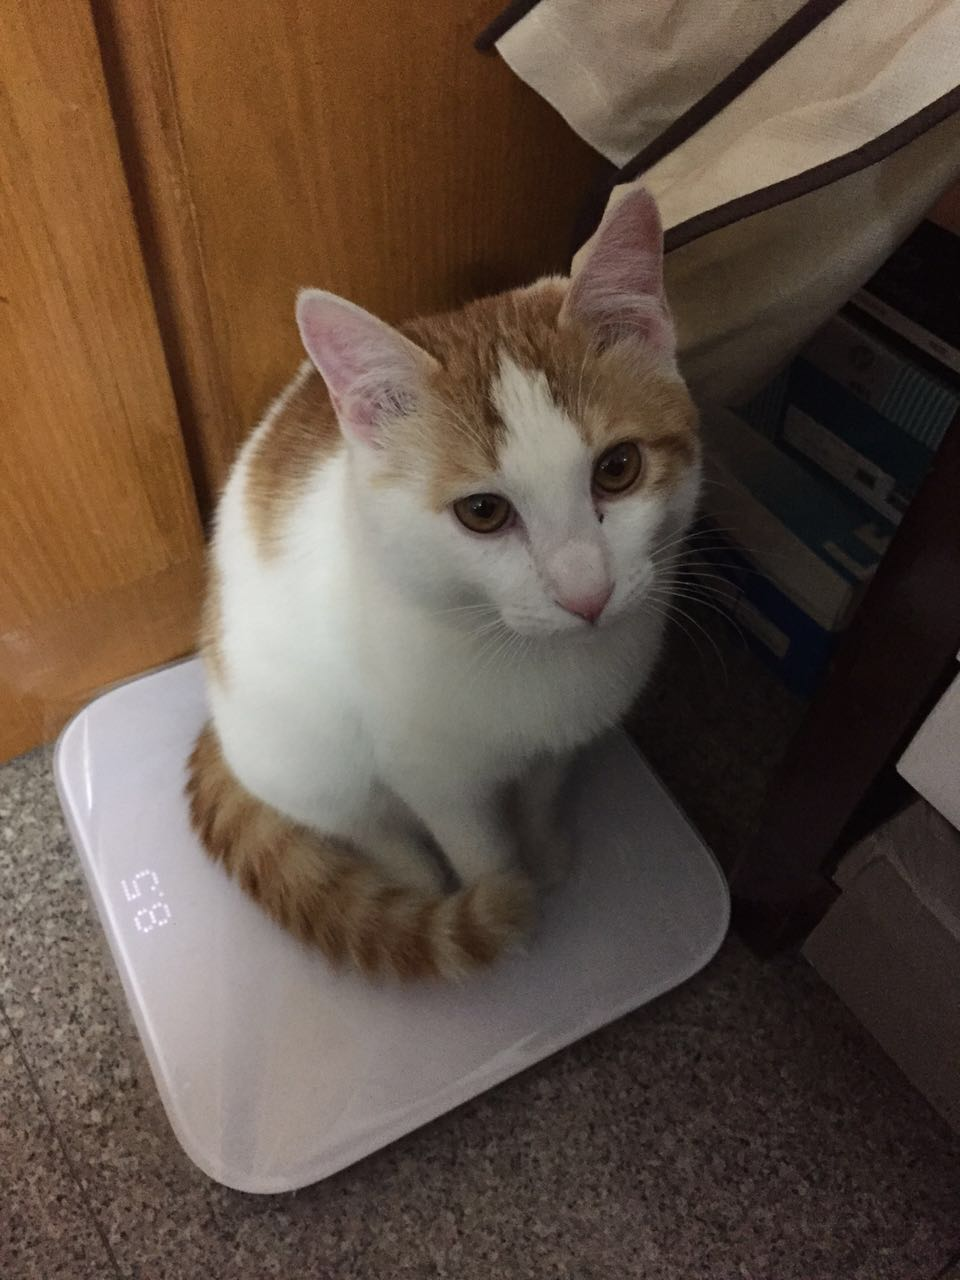
\includegraphics[width=0.3\textwidth]{./Figures/Prof-Miew.jpg}\par\vspace{1cm}
  {\LARGE 同济大学中德工程学院 \par}
  \vspace{1cm}
  {\scshape\Large CDHAW of Tongji University\par}
  \vspace{1.5cm}
  {\huge\bfseries DSGE模型笔记\par}
  \vspace{2cm}
  {\Large\itshape 朱彦元\par}
  \vfill
%  email address\par
  Dr.~Yanyuan \textsc{Zhu} \\
  \href{mailto:yyz@tongji.edu.cn}{yyz@tongji.edu.cn}
  \vfill

% Bottom of the page
  {\large \today\par}
\end{titlepage}

\tableofcontents{}

\chapter{前言}
还没想好要写什么...
\part{模型构建}
%!TEX root = ../DSGEnotes.tex
\chapter{基准New Keynesian模型}
\label{sec:Basic-NK-model}

\section{家庭部门}
\label{sec:Basic-NK-model-HH-sector}


假定cashless economy,家庭的效用函数$U(C_t, N_t)$表示为\footnote{膏按:RBC(DSGE)在经验研究中中常用工作小时数而非就业人员数作为$N_t$的代理变量,其相关讨论早期文献可见\cite{Hansen:1985ku,Rogerson:1988js};近期的综述见\cite{Rogerson:2009ez}。}
\begin{equation}
  \label{eq:utility-function}
  U(C_t, N_t) = \frac{C_t^{1-\sigma}}{1-\sigma} - \psi \cdot \frac{N_t^{1+\eta}}{1+\eta},
\end{equation}

HH问题。目标:追求效用最大化
\begin{align}
  \label{eq:HH-problem-max}
  \max_{\{C_t, N_t, B_{t+1}\}} & E_0 \sum_{t=0}^{\infty} \beta^t \cdot U(C_t, N_t), \nonumber \\
&st. \quad P_t \cdot C_t + B_{t+1} \le W_t \cdot N_t + Div_t - P_t \cdot T_t + (1+i_{t-1}) \cdot B_t,
\end{align}
其中$Div_t$表示dividends,中间产品企业的(垄断)利润。$T_t$表示税收或转移支付。$i_t$为名义利率。

建Lagrange
\begin{equation}
  \label{eq:HH-problem-lagrange}
  \mathcal{L} = E_0 \sum_{t=0}^{\infty} \beta^t \cdot \{ U(C_t, N_t) + \lambda_t \cdot \left[W_t \cdot N_t + Div_t - P_t \cdot T_t + (1+i_{t-1}) \cdot B_t - P_t \cdot C_t - B_{t+1}\right]\}.
\end{equation}

FOCs
\begin{align*}
  \frac{\partial \mathcal{L}}{\partial C_t}=0 &\Rightarrow C_t^{-\sigma} = \lambda_t \cdot P_t \\
  \frac{\partial \mathcal{L}}{\partial N_t}=0 & \Rightarrow \psi \cdot N_t^{\eta} = \lambda_t \cdot W_t \\
\frac{\partial \mathcal{L}}{\partial B_{t+1}}=0 & \Rightarrow \frac{\partial \{\lambda_t \cdot (1 + i_{t-1}) \cdot B_t\}}{\partial B_{t+1}} - \lambda_t = \frac{\partial \beta \cdot E_t \{ \lambda_{t+1} \cdot (1 + i_{t}) \cdot B_{t+1} \} } {\partial B_{t+1}} - \lambda_t = 0\\
\end{align*}

整理得
\begin{gather}
  \label{HH-FOC-labor-supply}
  \psi \cdot N_t^{\eta} = C_t^{-\sigma} \cdot w_t \\
\label{HH-FOC-euler-consumption}
  C_t^{-\sigma} = \beta \cdot E_t\{ C_{t+1}^{-\sigma} \cdot (1+i_t) \cdot \frac{P_t}{P_{t+1}}\}=\beta \cdot E_t\{ C_{t+1}^{-\sigma} \cdot (1+i_t) \cdot ( 1+\pi_{t+1} )^{-1}\},
\end{gather}
其中$w_t \equiv \frac{W_t}{P_t}$表示实际工资,$\pi_t \equiv P_t/P_{t-1}$表示通货膨胀率。由  \eqref{HH-FOC-labor-supply}可得Frisch elasticity of labor supply为$1/\eta$\footnote{假定短时期内家庭的总财富(总消费)不变,市场上工资的变化只影响家庭的劳动力供应,Frisch labor supply elasticity\citep{Frisch:1932wk,Frisch:1959jt}可表示为
  \begin{equation*}
    \frac{\partial n_t}{\partial w_t} \cdot \frac{w_t}{n_t},
  \end{equation*}
可参考\cite[pp.279]{Heer:2009ig},以及\cite{Christiano:2010wla}。}。



\section{企业部门}
\label{sec:Basic-NK-model-firm-sector}

\subsection{最终产品生产部门}
\label{sec:Basic-NK-model-final-produc-firm-sector}
最终产品部门以中间产品$Y_t(j), j \in [0,1]$的组合为投入要素,产出$Y_t$,符合完全竞争假定。\cite{Dixit:1977tv}形式的生产规模报酬不变生产函数为
\begin{equation}
  \label{eq:fin-prod-prod-func}
  Y_t = \left[ \int_{0}^{1} Y_t(j)^{\frac{\epsilon - 1}{\epsilon}} dj\right]^{\frac{\epsilon}{\epsilon - 1}},
\end{equation}
其中$\epsilon > 1$表示$j^{th}$中间产品的替代弹性。

最终产品厂商问题:在给定$P_t(j)$的情况下,通过选择$Y_t(j)$的投入追求利润最大化

\begin{equation}
  \label{eq:fin-prod-problem-max}
  \max_{Y_t(j)} P_t \cdot Y_t - \int_{0}^{1} P_t(j) \cdot Y_t(j) dj ,
\end{equation}

引入式\eqref{eq:fin-prod-prod-func},FOC整理可得对$j$中间产品的需求函数
\begin{equation}
  \label{eq:demand-for-intm-j}
  Y_t(j) = \left( \frac{P_t(j)}{P_t}
\right)^{-\epsilon} \cdot Y_t,
\end{equation}

进而根据完全竞争市场假定
\begin{equation*}
  \begin{split}
    P_t \cdot Y_t & \equiv \int_0^1 P_t(j) \cdot Y_t(j) dj \\
    &=\left[\int_0^1 \left(\frac{P_t(j)}{P_t}\right)^{-\epsilon} \cdot Y_t \cdot P_t(j) dj \right] \\
    &=\left[\int_0^1 P_t(j)^{1-\epsilon} dj \right] \cdot P_t^{\epsilon} \cdot Y_t,\\
  \end{split}
\end{equation*}
整理得最终产品价格的决定(aggregate price index):
\begin{equation}
  \label{eq:agg-price-index}
  P_t = \left[
    \int_0^1 P_t(j)^{1-\epsilon} dj
  \right]^{\frac{1}{1-\epsilon}}
\end{equation}

\subsection{中间产品生产部门}
\label{sec:Basic-NK-model-intm-produc-firm-sector}
中间产品生产部门假定处于垄断竞争状态。代表企业$j$雇佣劳动力$N_t(j)$生产$Y_t(j)$,生产函数形式
\begin{equation}
  \label{eq:intm-prodc-func}
  Y_t(j) = A_t \cdot N_t(j),
\end{equation}
其中$A_t$表示外生的生产率冲击,它对所有中间产品生产者都是相同的。对劳动力的总需求为$j$个厂商的加总。
\begin{equation}
  \label{eq:Labor-D-S}
  N_t = \int_0^1 N_t(j)dj.
\end{equation}

\subsubsection{成本最小化:边际成本与工资}
\label{sec:intm-min-cost}
中间产品生产者$j$的问题可以表示为两阶段优化。第一阶段为成本最小化:在给定工资$W_t$的基础上,选择雇佣劳动力投入$N_t(j)$,生产中间品$Y_t(j)$,以满足最终产品生产部门对$Y_t(j)$的需求,
\begin{equation}
  \label{eq:intm-prod-max-N}
  \begin{split}
      \min_{N_t(j)} &W_t \cdot N_t(j),\\
      &st. \quad A_t \cdot N_t(j) \ge \left( \frac{P_t(j)}{P_t}\right)^{-\epsilon} Y_t,
  \end{split}
\end{equation}
第二行LHS和RHS分别表示中间产品$Y_t(j)$的供应和需求,见式\eqref{eq:intm-prodc-func}和式 \eqref{eq:demand-for-intm-j}。

建Lagrange
\begin{equation*}
  \mathcal{L} = W_t \cdot N_t(j) + \lambda_t \cdot \left[
\left(\frac{P_t(j)}{P_t}\right)^{-\epsilon} \cdot Y_t - A_t \cdot N_t(j)
\right],
\end{equation*}
其中拉格朗日乘子$\lambda_t$表示$j$生产额外1单位$Y_t(j)$的影子价格(边际成本),设为$MC_t \equiv \lambda_t $.

FOC:
\begin{equation*}
  MC_t = \frac{W_t}{A_t}
\end{equation*}

或者用实际价格形式表示
\begin{equation}
  \label{eq:intm-prod-min-N-mc}
    mc_t = \frac{MC_t}{P_t} = \frac{W_t}{A_t \cdot P_t} = \frac{w_t}{A_t}.
\end{equation}

式\eqref{eq:intm-prod-min-N-mc}  反映了实际(边际成本)和实际工资的对应关系。

\subsubsection{利润最大化:定价策略}
\label{sec:intm-max-profit}
在此基础上,第二阶段,中间产品生产者$j$对自己的产品$Y_t(j)$定价$P_t(j)$,以追求实际利润$\Pi_t$最大化。
\begin{equation}
  \label{eq:intm-prod-profit}
  \begin{split}
    \Pi_t(j) &= \frac{P_t(j) \cdot Y_t(j)}{P_t} - \frac{W_t \cdot N_t(j)}{P_t} \\
    &=\frac{P_t(j)}{P_t} \cdot Y_t(j) - mc_t \cdot Y_t(j) \\
    &=\left( \frac{P_t(j)}{P_t}\right)^{1-\epsilon} \cdot Y_t - mc_t \cdot \left( \frac{P_t(j)}{P_t}\right)^{-\epsilon} \cdot Y_t
  \end{split}
\end{equation}

粘性价格。在$t$时期,中间产品生产者$j$ 有$\phi<1$的概率不能调整价格,维持上一期的定价$P_{t-1}(j)$;有$1-\phi$的概率可以调整价格,将产品售价更新为$P_t^{\#}(j)$。
\begin{equation}
  \label{eq:intm-stick-prices}
  P_t(j) =
  \begin{cases} P_{t-1}(j) &\mbox{with prob.} \quad \phi \\
    P_t^{\#}(j) & \mbox{else} \quad 1-\phi
\end{cases}
\end{equation}

根据模型假设,中间产品生产部门由于垄断产生的利润$\Pi_t$,流回到家庭部门,供消费以提升效用,满足跨期消费的Euler equation式\eqref{HH-FOC-euler-consumption},设$\widetilde{M}_{t+s} \equiv \beta^s \cdot \frac{U_{C,t+s}}{U_{C,t}}$作为discount factor。从$t$期向前直到$t+s$期,$j$不能自由调整价格的概率是$\phi^s$。此外,从$t$期向前直到$t+s$期,$j$不能自由调整价格的概率是$\phi^s$。
由此,$j$生产者forward-looking的随机折旧因子为$\phi^s \cdot \widetilde{M}_{t+s}$。

先来看式\eqref{eq:intm-stick-prices}中$p^{\#}_j(j)$的决定。$t$期中间品生产者$j$的利润最大化问题表示为
\begin{equation*}
  \begin{split}
    &\max_{P_t(j)} E_t \sum_{s=0}^{\infty} \phi^s \cdot \widetilde{M}_{t+s} \cdot \Pi_{t+s} \\
    &=\max_{P_t(j)} E_t \sum_{s=0}^{\infty} \left(\beta \cdot \phi \right)^s \cdot \frac{U_{C,t+s}}{U_{C,t}} \cdot \left[
      \frac{P_{t+s}(j)}{P_{t+s}} \cdot Y_{t+s}(j) - mc_{t+s} \cdot Y_{t+s}(j)
    \right]\\
    &=\max_{P_t(j)} E_t \sum_{s=0}^{\infty} \left(\beta \cdot \phi \right)^s \cdot \frac{U_{C,t+s}}{U_{C,t}} \cdot Y_{t+s} \cdot
    \left[
      \left( \frac{P_{t}(j)}{P_{t+s}} \right)^{1-\epsilon} - mc_{t+s} \cdot \left( \frac{P_{t}(j)}{P_{t+s}} \right)^{-\epsilon}
    \right],
  \end{split}
\end{equation*}

FOC wrt $P_{t}(j)$,整理得
\begin{equation}
  \label{eq:intm-update-price-principle}
  P_{t}(j) = \frac{\epsilon}{\epsilon -1} \cdot \frac
{
  E_t \sum_{s=0}^{\infty} \left(\beta \cdot \phi \right)^s \cdot U_{C,t+s} \cdot Y_{t+s} \cdot mc_{t+s} \cdot P_{t+s}^{\epsilon}
}
{
  E_t \sum_{s=0}^{\infty} \left(\beta \cdot \phi \right)^s \cdot U_{C,t+s} \cdot Y_{t+s} \cdot P_{t+s}^{\epsilon-1}
}
\end{equation}
式\eqref{eq:intm-update-price-principle} RHS分子和分母均与$j$无关,即在价格粘性的情况下,forward-looking的所有中间产品生产者$j\in[0,1]$,如果有机会调整价格(概率$1-\phi$),都会遵循相同的价格调整策略,设为$P^{\#}_{t} \equiv P^{\#}_{t}(j), \forall j$。上式改写为

\begin{equation}
  \label{eq:intm-update-price-aux}
  P^{\#}_t = \frac{\epsilon}{\epsilon  -1} \cdot \frac{X_{1,t}}{X_{2,t}},
\end{equation}
其中辅助变量
\begin{align}
\label{auxiliary-X1}
  X_{1,t} &\equiv U_{C,t} \cdot Y_t \cdot P_{t}^{\epsilon} \cdot mc_t + \beta \cdot \phi \cdot E_t X_{1,t+1},\\
\label{auxiliary-X2}
  X_{2,t} &\equiv U_{C,t} \cdot Y_t \cdot P_{t}^{\epsilon-1} + \beta \cdot \phi \cdot E_t X_{2,t+1}.
\end{align}

为了让变量平稳,定义$x_{1,t} \equiv X_{1,t}/P_{t}^{\epsilon}$,$x_{2,t} \equiv X_{2,t}/P_{t}^{\epsilon-1}$,式  \eqref{eq:intm-update-price-aux}变为
\begin{equation}
  \label{eq:intm-update-price-aux-stationary}
  P^{\#}_t = \frac{\epsilon}{\epsilon  -1} \cdot \frac{x_{1,t}}{x_{2,t}} \cdot P_t.
\end{equation}

或者定义reset price的通胀项$(1+ \pi^{\#}_t) \equiv P^{\#}_t / P_{t-1}$,将式\eqref{eq:intm-update-price-aux-stationary}由价格形式改写为通货膨胀率的形式
\begin{equation}
  \label{eq:intm-update-inflation-aux}
  (1+\pi^{\#}_t) = \frac{\epsilon}{\epsilon -1} \cdot \left( 1+\pi_t \right) \cdot \frac{x_{1,t}}{x_{2,t}}.
\end{equation}

根据\eqref{eq:intm-update-price-aux-stationary},在flexible price即$\phi =0$的情况下,$\forall j$ 中间产品的定价为$P^{\#}_t = \frac{\epsilon}{\epsilon -1} \cdot (mc_t \cdot P_t)$,即名义的边际成本乘以markup。


\subsection{最终产品定价:Calvo assupmtion}
\label{sec:final-produc-price}

Aggregate price index 式\eqref{eq:agg-price-index}中含有$j$,为了消除中间产品生产者的价格异质性对最终产品价格的影响,引入式\eqref{eq:intm-stick-prices},根据Calvo assumption \citep{Calvo:1983uqa}得
\begin{align}
\label{eq:agg-price-index-noj}
  P_t^{1-\epsilon} &= \int_{0}^1 P_t(j)^{1-\epsilon} dj \nonumber\\
                   &= \int_{0}^{1-\phi} \left(P_t^{\#}\right)^{1-\epsilon} dj + \int_{1-\phi}^1 \left(P_{t-1}(j)\right)^{1-\epsilon} dj\nonumber\\
                   &= \int_{0}^{1-\phi} \left(P_t^{\#}\right)^{1-\epsilon} dj + \int_{0}^{\phi} \left(P_{t-1}(j)\right)^{1-\epsilon} dj\nonumber\\
                   &= (1-\phi) \cdot \int_{0}^{1} \left(P_t^{\#}\right)^{1-\epsilon} dj + \phi \cdot \int_{0}^1 \left(P_{t-1}(j)\right)^{1-\epsilon} dj \nonumber\\
                   &=(1-\phi) \cdot \left(P^{\#}_t\right)^{1-\epsilon} + \phi \cdot \left(P_{t-1}\right)^{1-\epsilon}
\end{align}

或者以reset price inflation形式表示为
\begin{equation}
  \label{eq:agg-inflation-index}
  \left(1+\pi_t\right)^{1-\epsilon} = (1-\phi) \cdot \left(1+\pi^{\#}_t\right)^{1-\epsilon} + \phi
\end{equation}

\section{外生技术冲击}
\label{sec:exo-prod-shock}
设外生技术冲击满足$\log$形式的AR(1)过程
\begin{equation}
  \label{eq:exo-prod-shock}
  \ln A_t = \rho_a \cdot \ln A_{t-1} + \varepsilon_{a,t}
\end{equation}
其中$0<\rho_a<1$,$E\{\varepsilon_{a,t}\}=0$。

\section{总量均衡}
\label{sec:Equilibrium-cond}



\subsection{家庭部门消费的决定}
\label{equilibrium-cond-HH-consumption}
均衡状态下,家庭持有的债券和净转移支付为零,$B_t=T_t = 0$ $\forall t$。$Div_t$来自全部中间产品生产者的垄断利润之和,
\begin{equation}
  \label{eq:quili-cond-HH-Div-Pi}
\begin{split}
  \frac{Div_t}{P_t} &= \frac{\Pi_t}{P_t} \\
  &\equiv \int_{0}^1 \left[ \frac{P_t(j)}{P_t} \cdot Y_t(j) - \frac{W_t}{P_t} N_t(j) \right] dj \\
  &= \int_{0}^1 \left( \frac{P_t(j)}{P_t} \right) Y_t(j) dj - w_t \cdot \int_{0}^1 N_t(j) dj \\
  &= \int_{0}^1 \left( \frac{P_t(j)}{P_t} \right) Y_t(j) dj - w_t \cdot N_t
\end{split}
\end{equation}

家庭部门预算约束条件式\eqref{eq:HH-problem-max}因此改写为
\begin{equation}
  \label{eq:HH-problem-C-Y}
  \begin{split}
      C_t &= \int_0^1  \left( \frac{P_t(j)}{P_t}\right) \cdot Y_t(j) dj \\
      &=\int_0^1  \left( \frac{P_t(j)}{P_t}\right) \cdot \left[ \left( \frac{P_t(j)}{P_t}\right)^{-\epsilon} \cdot Y_t \right]\\
      &=\left[Y_t \cdot P_t^{\epsilon -1}\right] \cdot \int_{0}^1 P_t(j)^{1-\epsilon} dj \\
      &=Y_t
  \end{split}
\end{equation}

\subsection{price dispersion}
在市场出清情况下,对$j$类中间产品$Y_t(j)$的需求式\eqref{eq:demand-for-intm-j}与供应式\eqref{eq:intm-prodc-func}联立,并加总
\begin{equation*}
  \int_{0}^1 A_t \cdot N_t(j) dj= \int_0^1 \left(\frac{P_{t}(j)}{P_t}\right)^{-\epsilon} \cdot Y(t) dj,
\end{equation*}
整理可得(最终产品)总量生产函数
\begin{equation}
  \label{eq:equili-agg-j-prod-DS}
  Y_t = \frac{A_t \cdot N_t}{\nu^p_t},
\end{equation}
其中$\nu^p_t \ge 1$
\begin{equation}
  \label{eq:price-dispersion-index}
  \nu^p_t = \int_0^1 \left(\frac{P_t(j)}{P_t}\right)^{-\epsilon} dj
\end{equation}
是price dispersion index,反映市场上各种商品价格的差异程度:价格不一致的程度越高,$v_t^p$越大,总产出越小;lower bound $\nu_t^p=1$表示在没有price friction时,所有企业对自己的产品都会设定同样的价格。这在一定程度上说明了旨在稳定物价政策的重要性。

利用Calvo assumption对$\nu^p_t$作调整,以消除$j$个体企业的异质性:

\begin{align}
\label{eq:price-dispersion-index-noj}
  \nu^p_t &= \int_{0}^{1-\phi} \left(\frac{P_t^{\#}}{P_t}\right)^{-\epsilon} dj + \int_{1-\phi}^1 \left(\frac{P_{t-1}(j)}{P_t}\right)^{-\epsilon} dj\nonumber\\
                   &= (1-\phi) \cdot \int_{0}^{1} \left(\frac{P_t^{\#}}{P_{t-1}}\right)^{-\epsilon}
\cdot \left(\frac{P_t}{P_{t-1}}\right)^{\epsilon} dj + \phi \cdot \int_{0}^{1} \left(\frac{P_{t-1}(j)}{P_{t-1}}\right)^{-\epsilon} \cdot \left(\frac{P_t}{P_{t-1}}\right)^{\epsilon} dj\nonumber\\
                   &= (1-\phi) \cdot (1+\pi^{\#}_t)^{-\epsilon} \cdot (1+\pi_t)^{\epsilon} + \phi \cdot (1+\pi_t)^{\epsilon} \cdot \int_{0}^1 \left(\frac{P_{t-1}(j)}{P_{t-1}}\right)^{-\epsilon} dj \nonumber\\
                   &=(1-\phi) \cdot (1+\pi^{\#}_t)^{-\epsilon} \cdot (1+\pi_t)^{\epsilon} + \phi \cdot (1+\pi_t)^{\epsilon} \cdot \nu^p_{t-1}.
\end{align}

\section{(非随机的)稳定状态}
\label{sec:BNK-steady-state}
根据第\ref{sec:Equilibrium-cond}节的总量均衡,可以进一步探讨非随机稳态。我们将未标注时间下角标的变量表示为其稳定状态。

根据定义式\eqref{eq:exo-prod-shock}可得
\begin{equation}
  \label{eq:ss-A}
  A=1.
\end{equation}

式\eqref{eq:HH-problem-C-Y} $\Rightarrow$
\begin{equation}
  \label{eq:ss-C-Y}
  Y=C.
\end{equation}

跨期消费的Euler等式\eqref{HH-FOC-euler-consumption} $\Rightarrow$
  \begin{align}
  \label{eq:ss-interest-rate}
      i &= \frac{1-\beta}{\beta} + \frac{1}{\beta} \cdot \pi \nonumber \\
        &\approx \rho + \pi,
  \end{align}
上式中第二行等式,假定时间贴现$\beta \approx 1$,则$ \rho \equiv \frac{1-\beta}{\beta}$表示时间贴现率。

Reset price inflation 式\eqref{eq:agg-inflation-index} $\Rightarrow$
\begin{equation}
  \label{eq:ss-reset-price-inflation}
  (1+\pi^{\#}) = \left[
    \frac{(1+\pi)^{1-\epsilon} - \phi}{1-\phi}
  \right]^{\frac{1}{1-\epsilon}}.
\end{equation}

price dispersion 式\eqref{eq:price-dispersion-index-noj} $\Rightarrow$
\begin{equation}
  \label{eq:ss-price-dispersion-index}
  \nu^p = \frac{(1-\phi) \cdot \left[\frac{1+\pi}{1+\pi^{\#}} \right]^{\epsilon}}{1-\phi \cdot (1+\pi)^{\epsilon}}.
\end{equation}

边际成本式\eqref{eq:intm-update-inflation-aux} $\Rightarrow$
\begin{equation}
  \label{eq:ss-marginal-cost}
  mc = \frac{1-\phi \cdot \beta \cdot (1+\pi)^{\epsilon}}{1-\phi \cdot \beta \cdot (1+\pi)^{\epsilon-1}} \cdot \frac{1+\pi^{\#}}{1+\pi} \cdot \frac{\epsilon -1}{\epsilon}
\end{equation}

基于式\eqref{eq:ss-reset-price-inflation}、\eqref{eq:ss-price-dispersion-index}和\eqref{eq:ss-marginal-cost},利用数值模拟的方法,考察稳态下总物价通胀$\pi$和reset price通胀$\pi^{\#}$、price dispersion$v^p$、边际成本$mc$之间的关系。

\begin{enumerate}
\item $\pi=0$时,$\pi^{\#}=0$。$\pi \gtrless 0$时,$\pi^{\#} \gtrless \pi$。见图\ref{fig:simul-pi-pisharp-nup}左图。
\item $\pi=0$时,$\nu^p=1$,price dispersion处于最小值。$\pi \neq 0$时,$\nu^{p} > 1$,且相比较负通胀($\pi <0$),$\nu^p$对正通胀的响应更剧烈,导致对产出的干扰更大。见图\ref{fig:simul-pi-pisharp-nup}中图。
\item $\pi = 0$时,$mc=\frac{\epsilon-1}{\epsilon}$,即等于fixed price markup的倒数。$\pi \neq 0$时,有$mc < \frac{\epsilon -1}{\epsilon}$,说明$\pi \neq 0$时的steady state markup,大于$\pi = 0$时的steady state price markup。见图\ref{fig:simul-pi-pisharp-nup}右图。
\end{enumerate}


\begin{figure}[p]
  \centering
  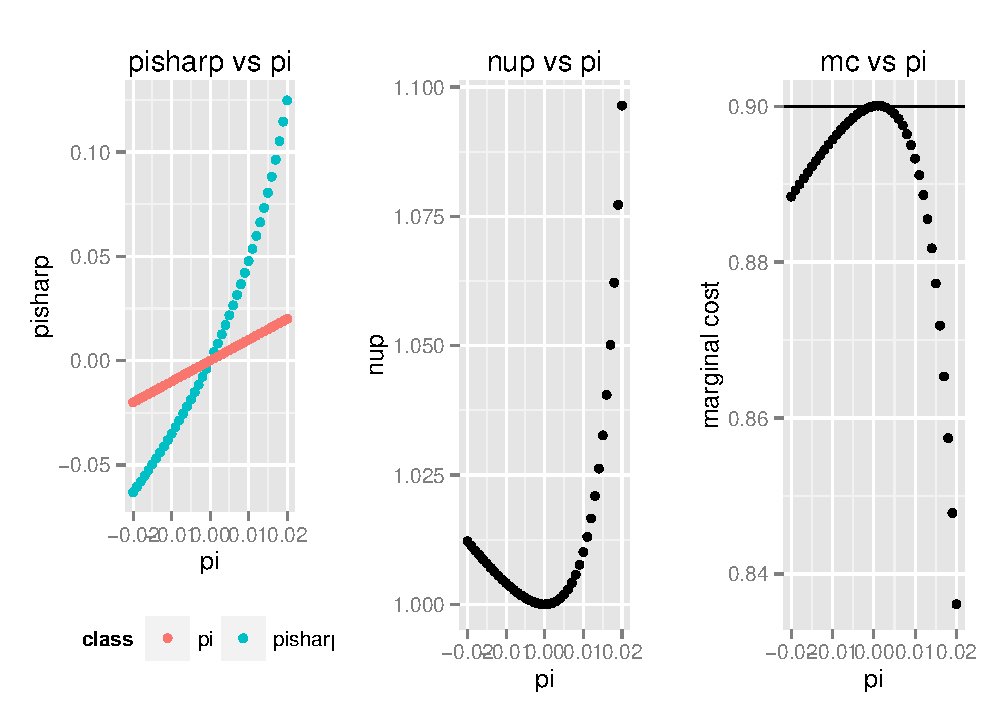
\includegraphics[width=0.8\textwidth]{Figures/R-simul-pi-pisharp-nup.pdf}
  \caption{数值模拟:$\{\pi^{\#},\nu^p\}$ vs $\pi$。模拟过程中设参数值$\phi=0.25$,$\epsilon=10$, $\beta = 0.99$。}
  \label{fig:simul-pi-pisharp-nup}
\end{figure}

给定$A=1$,工资决定式\eqref{eq:intm-prod-min-N-mc} $\Rightarrow$
\begin{equation}
  \label{eq:ss-wage}
  w = mc
\end{equation}
即工资等于劳动投入的边际成本。

式\eqref{eq:equili-agg-j-prod-DS} $\Rightarrow$ 边际产出$mpn$
\begin{equation}
  \label{eq:ss-mpn}
  mpn = \frac{1}{\nu^p}
\end{equation}
可见$\pi=0$时,mpn和mc的差距最小,体现为一个fixed price markup $\frac{\epsilon}{\epsilon -1}$。$\pi \neq 0$且越远离0时,经济体distorted的程度越大;此外,$\pi>0$时经济体的distorted程度,高于$\pi<0$时。

劳动力的供应式\eqref{HH-FOC-labor-supply} $\Rightarrow$
\begin{align*}
  \psi \cdot N^{\eta} &= C^{-\sigma} \cdot w \\
                      &= Y^{-\sigma} \cdot mc \\
                      &= \left(\frac{N}{\nu^p}\right)^{-\sigma} \cdot mc,
\end{align*}
整理得
\begin{equation}
  \label{eq:ss-labor-supply}
  N = \left[ \frac{1}{\psi} \cdot \left( \nu^p \right)^{\sigma} \cdot mc \right] ^{\frac{1}{\eta + \sigma}}
\end{equation}

总产出由式\eqref{eq:equili-agg-j-prod-DS}   \eqref{eq:ss-labor-supply}   \eqref{eq:ss-marginal-cost}得 $\Rightarrow$
\begin{align}
  \label{eq:ss-agg-output}
  Y &= \frac{N}{\nu^p},\nonumber \\
      &= \frac{\left[ \frac{1}{\psi} \cdot \left( \nu^p \right)^{\sigma} \cdot mc \right] ^{\frac{1}{\eta + \sigma}}}{\nu^p} \nonumber \\
      &= \left(\frac{1}{\psi}\right)^{\frac{1}{\sigma + \eta}} \cdot \left( v^p \right)^{-\frac{\eta}{\eta + \sigma}} \cdot
        \left[
        \frac{1-\phi \cdot \beta \cdot (1+\pi)^{\epsilon}}{1-\phi \cdot \beta \cdot (1+\pi)^{\epsilon-1}} \cdot \frac{1+\pi^{\#}}{1+\pi} \cdot \frac{\epsilon -1}{\epsilon}
        \right]^{\frac{1}{\eta + \sigma}}
\end{align}

\section{flexible price equilibrium 和 output gap}
\label{sec:flexible-price-output-gap}
\subsection{flexible price equilibrium}
\label{sec:flexible-price}

假定中间产品生产者可以自由调整价格,对应$\phi = 0$。将变量加上角标$f$以标注。此时$\pi = \pi^{\#}$,且名义价格不会对实际变量产生任何影响。

Flexible price dispersion index式\eqref{eq:price-dispersion-index-noj} $\Rightarrow$
\begin{equation}
  \label{eq:flexible-price-dispersion-index}
  v_t^{p,f} = 1,
\end{equation}
即包括最终产品和中间产品在内的全部生产者都会采取同样的产品定价策略,使price dispersion位于最低值1。

Reset price inflation 式\eqref{eq:intm-update-inflation-aux} $\Rightarrow$
\begin{equation}
  \label{eq:flexible-price-marg-cost}
  mc_t^f = \frac{\epsilon - 1}{\epsilon},
\end{equation}
可见边际成本是price markup的倒数。企业的定价策略在于:给$mc$加上一个固定的fixed price markup权数,作为产品售价。

Flexible price wage $\Rightarrow$
\begin{align*}
  mpn_t^f &= \frac{\partial Y_t^f}{\partial N_t^f} = A_t, \\
  P_t^f &= mc_t^f \cdot \frac{\epsilon}{\epsilon-1},\\
  mc_t^f &= w_t,\\
  mpn_t &= p_t^f,
\end{align*}
整理得
\begin{equation}
  \label{eq:flexible-price-wage}
  w_t^f = A_t \cdot \frac{\epsilon-1}{\epsilon}.
\end{equation}

Flexible price labor supply $\Rightarrow$
\begin{align*}
  \psi (N_t^f)^{\eta} &= (C_t^f)^{-\sigma} \cdot w_t^f,\\
                      &=(Y_t^f)^{-\sigma} \cdot mc_t^f,\\
                      &=\left( A_t \cdot N_t^f \right)^{-\sigma} \cdot \left( \frac{\epsilon -1}{\epsilon} \cdot A_t\right),
\end{align*}
整理得
\begin{equation}
  \label{eq:flexible-price-labor-supply}
  N_t^f = \left(\frac{1}{\psi} \cdot \frac{\epsilon -1}{\epsilon} \cdot A_t^{1-\sigma}\right)^{\frac{1}{\sigma + \eta}}.
\end{equation}

Flexible price aggregate output $\Rightarrow $
\begin{equation}
  \label{eq:flexible-price-agg-output}
  Y_t^f = A_t \cdot N_t^f = \left(\frac{1}{\psi} \cdot \frac{\epsilon -1}{\epsilon}\right)^{\frac{1}{\sigma + \eta}} \cdot  A_t^{\frac{1+\eta}{\sigma + \eta}}
\end{equation}

可见flexible price $(\phi =0)$情况下,名义波动不会对真实变量产生影响。

\subsection{output gap}
\label{output-gap}
定义output gap $\ln X_t \equiv \ln Y_t - \ln Y_t^f$,表示flexible price $(\phi = 0)$情况下产出$Y_t^f$与sticky price $(\phi >0)$情况下产出$Y_t$的差。

稳定状态下,$Y^f$的值由式\eqref{eq:flexible-price-agg-output}给出;
\begin{equation*}
%\label{ss-flexible-price-agg-output}
    Y^f = \left(\frac{1}{\psi} \cdot \frac{\epsilon -1}{\epsilon}\right)^{\frac{1}{\sigma + \eta}}
\end{equation*}

由此可得稳态output gap的值:
\begin{equation}
  \label{eq:ss-output-gap}
  \frac{Y}{Y^f} =
  \left[
    \frac{1-\phi \cdot \beta \cdot (1+\pi)^{\epsilon}}{1-\phi \cdot \beta \cdot (1+\pi)^{\epsilon -1}} \cdot \frac{1+\pi^{\#}}{1+\pi}
  \right]^{\frac{1}{\eta + \sigma}} \cdot
  \left(
    \nu^p
  \right)^{- \frac{\eta}{\eta + \sigma}}
\end{equation}
output gap的性质,分两种情况来讨论:

\begin{enumerate}
\item $\pi = 0$ $\Rightarrow$ $\pi^{\#} = \pi = 0$,$\nu^p = 1$ $\Rightarrow$ $Y=Y^f$ $\Rightarrow$ $\ln X = 0$,
\item $\pi >0$ $\Rightarrow$ $\pi^{\#} > \pi$, $\nu^p >1$ $\Rightarrow$ $Y<Y^f$ $\Rightarrow$ $\ln X < 0$。
\end{enumerate}
即在sticky price $(\phi >0)$条件下,稳态的output gap(对数)为负。


\section{Taylor法则}
\label{seq:Taylor-Rule}
假定中央银行的货币政策着眼于利率而非货币供应量:通过盯紧通货膨胀和产出这两个变量,灵活制定内生的货币政策以达到既定的利率目标\footnote{膏按:外生利率政策会导致indeterminacy问题,补充一个Appendix。}。常见的内生货币政策如Taylor法则:

\begin{equation}
  \label{eq:MP-Taylor-Rule}
  (i_t-i) = \rho_i \cdot (i_{t-1}-i) + (1-\rho_i) \cdot i+ (1-\rho_i) \cdot \left[
    \theta_{\pi} \cdot (\pi_t - \pi) + \theta_{x} \cdot (\ln X_t - \ln X)
  \right] + \varepsilon_{i,t},
\end{equation}
其中$i_t$表示名义利率。$X_t$表示output gap,见第\ref{output-gap}节。去掉下角标的变量表示其稳态值。$0 \le \rho_i \le 1$表示smoothing parameter。$\theta_\pi \ge 0$,$\theta_{x} \ge 0$。外生利率冲击$E\{ \varepsilon_{i,t}\} = 0$。

不难看出式\eqref{eq:MP-Taylor-Rule}的Taylor法则是个局部调整的货币政策:如果将稳态值$i$和$\pi$视作长期目标,则中央银行根据上期名义利率(距其稳态值)的偏离程度,以及当前期目标值(距其稳态值)的偏离程度,来灵活调整当期的名义利率;当前期目标值包括通货膨胀和output gap。一旦当期名义利率的调整目标确定,中央银行即通过向市场印发货币等手段,调节市场上的货币量,来实现其名义利率的目标。

\section{完整的均衡条件}
\label{sec:full-set-equilibrium-conditions}
经济系统的均衡解包括下述12个变量$\{ C_t, N_t, w_t, mc_t, Y_t, v^p_t, i_t, \pi_t, \pi^{\#}_t, x_{1,t}, x_{2,t}, A_t \}$,以及12个等式:

跨期消费的Euler equation 式\eqref{HH-FOC-euler-consumption} $\Rightarrow$
\begin{equation*}
    C_t^{-\sigma} = \beta \cdot E_t\{ C_{t+1}^{-\sigma} \cdot (1+i_t) \cdot \frac{P_t}{P_{t+1}}\}=\beta \cdot E_t\{ C_{t+1}^{-\sigma} \cdot (1+i_t) \cdot ( 1+\pi_{t+1} )^{-1}\}.
\end{equation*}

劳动力供应式\eqref{HH-FOC-labor-supply} $\Rightarrow$
\begin{equation*}
    \psi \cdot N_t^{\eta} = C_t^{-\sigma} \cdot w_t.
\end{equation*}

工资/边际成本的决定式\eqref{eq:intm-prod-min-N-mc} $\Rightarrow$
\begin{equation*}
    mc_t = \frac{MC_t}{P_t} = \frac{W_t}{A_t \cdot P_t} = \frac{w_t}{A_t}.
\end{equation*}

总消费与总产出的关系式\eqref{eq:HH-problem-C-Y} $\Rightarrow$
\begin{equation*}
  C_t = Y_t.
\end{equation*}

总量生产函数式\eqref{eq:equili-agg-j-prod-DS} $\Rightarrow$
\begin{equation*}
  Y_t = \frac{A_t \cdot N_t}{\nu^p_t}.
\end{equation*}

Price dispersion index 式\eqref{eq:price-dispersion-index-noj} $\Rightarrow$
\begin{equation*}
  \nu^p_t = (1-\phi) \cdot (1+\pi^{\#}_t)^{-\epsilon} \cdot (1+\pi_t)^{\epsilon} + \phi \cdot (1+\pi_t)^{\epsilon} \cdot \nu^p_{t-1}.
\end{equation*}

Evolution of inflation 式\eqref{eq:agg-inflation-index} $\Rightarrow$
\begin{equation*}
    \left(1+\pi_t\right)^{1-\epsilon} = (1-\phi) \cdot \left(1+\pi^{\#}_t\right)^{1-\epsilon} + \phi.
\end{equation*}

Reset price inflation 式  \eqref{eq:intm-update-inflation-aux} $\Rightarrow$
\begin{equation*}
  (1+\pi^{\#}_t) = \frac{\epsilon}{\epsilon -1} \cdot \left( 1+\pi_t \right) \cdot \frac{x_{1,t}}{x_{2,t}}.
\end{equation*}

两个reset price inflation的辅助变量,式\eqref{auxiliary-X1}-\eqref{auxiliary-X2} $\Rightarrow$
\begin{align*}
  x_{1,t} &\equiv C_t^{-\sigma} \cdot Y_t \cdot mc_t + \beta \cdot \phi \cdot E_t \left(1+\pi_{t+1} \right)^{\epsilon} \cdot x_{1,t+1},\\
  x_{2,t} &\equiv C_t^{-\sigma} \cdot Y_t + \beta \cdot \phi \cdot E_t \left( 1+\pi_{t+1} \right)^{\epsilon -1} \cdot x_{2,t+1}.
\end{align*}

Taylor rule 式\eqref{eq:MP-Taylor-Rule} $\Rightarrow$
\begin{equation*}
  (i_t-i) = \rho_i \cdot (i_{t-1}-i) + (1-\rho_i) \cdot i+ (1-\rho_i) \cdot \left[
    \theta_{\pi} \cdot (\pi_t - \pi) + \theta_{x} \cdot (\ln X_t - \ln X)
  \right] + \varepsilon_{i,t}.
\end{equation*}

Exogenous productivity shock 式\eqref{eq:exo-prod-shock} $\Rightarrow$
\begin{equation*}
  \ln A_t = \rho_a \cdot \ln A_{t-1} + \varepsilon_{a,t} .
\end{equation*}

\section{对数线性化}
\label{sec:BNK-log-lin-system}
\subsection{对数线性化计算}
\label{sec:BNK-log-linearization}
求解上述均衡方程组,方法之一是利用Dynare等计算机软件进行计算。此外,在模型较简单的情况下,也可以围绕zero-inflation steady state $\pi=0$的点,手算对数线性化的近似。

Euler equation 式\eqref{HH-FOC-euler-consumption} + 式\eqref{eq:HH-problem-C-Y} $\Rightarrow$
\begin{equation*}
  -\sigma \cdot \ln Y_t = \ln \beta - \sigma E_t \ln Y_{t+1} + i_t - E_t \pi_{t+1},
\end{equation*}
设$\ln (1+i_t) \approx i_t$,$\ln (1+\pi_t) \approx \pi_t$。将上式中每个变量分别围绕自己的稳态值作一阶泰勒级数展开,
\begin{equation*}
  -\sigma \cdot \frac{Y_t - Y}{Y} = -\sigma \cdot E_t \frac{Y_{t+1} - Y}{Y} + (i_t - i) - E_t (\pi_{t+1} - \pi),
\end{equation*}
定义$\tilde{Z}_t \equiv (Z_t - Z)/Z$作为变量$Z_t$距离其稳态值$Z$的偏离程度,$Z_t=(Y_t,N_t,A_t,\ldots)$;为了手算方便,对于已经是rate form的变量,包括利率$i_t$、通货膨胀率$\pi_t$和$\pi^{\#}_t$、price dispersion index $v^p_{t}$,直接用差分代替增速形式,如$\tilde{i}_t \equiv i_t -i$。上式进一步改写为
\begin{equation}
  \label{eq:log-lin-euler}
  \tilde{Y}_t = E_t \tilde{Y}_{t+1} - \frac{1}{\sigma} \left[\tilde{i}_t - E_t \tilde{\pi}_{t+1}\right].
\end{equation}

式\eqref{eq:log-lin-euler}又被称为New Keynesian IS Curve (NKIS)。Keynesian IS curve反映了投资(Investment)和投资(Saving)之间的对应关系。这里的“基础”New Keynesian模型中并未考虑投资,它反映了当期消费需求和实际之间的负相关关系。与传统IS curve相比,NKIS的“新”体现在其forward-looking的特征上:当期需求$(\tilde{C}_t = \tilde{Y}_t)$不只取决于实际利率$(\tilde{i}_t - E_t \tilde{\pi}_{t+1})$且负相关,还取决于对未来收入(消费)的期望$E_{t} \tilde {Y}_{t+1}$且负相关。

边际成本与工资的关系式\eqref{eq:intm-prod-min-N-mc} $\Rightarrow$
\begin{align}
  \tilde{mc}_t = \tilde{w}_t - \tilde{A}_t.
\end{align}

Price dispersion index 式\eqref{eq:price-dispersion-index-noj} $\Rightarrow$
\begin{align}
\label{eq:log-lin-price-dispersion-index}
  \tilde{\nu}^p_t &= \left[(-\epsilon) \cdot (1-\phi) \cdot (1+\pi^{\#})^{-\epsilon -1} \cdot (1+\pi)^{\epsilon}\right] \cdot (\pi^{\#}_t - \pi^{\#}) \nonumber\\
                    &+ \left[ \epsilon \cdot (1-\phi) \cdot (1+\pi^{\#})^{-\epsilon} \cdot (1+\pi)^{\epsilon -1} \right] \cdot \pi_t \nonumber\\
                    &+\left[ \epsilon \cdot \phi \cdot (1+\pi)^{\epsilon -1} \cdot \nu^p \right] \cdot (\pi_t - \pi) \nonumber\\
                    &+\left[ \phi \cdot (1+\pi)^{\epsilon} \right] \cdot \left(\nu^p_{t-1} - \nu^p \right) \nonumber\\
                  &=-\epsilon \cdot (1-\phi) \cdot \tilde{\pi}^{\#}_t + \epsilon \cdot (1-\phi) \cdot \tilde{\pi}_t + \epsilon \cdot \phi \cdot \tilde{\pi}_t + \phi \cdot \tilde{\nu}^p_{t-1} \nonumber\\
                    &=-\epsilon \cdot (1-\phi) \cdot \tilde{\pi}^{\#}_t + \epsilon \cdot \tilde{\pi}_t + \phi \cdot \tilde{\nu}^p_{t-1},
\end{align}
其中第三个等号用到$\pi = \pi^{\#} = 0$的假设条件。


Evolution of inflation 式\eqref{eq:agg-inflation-index} $\Rightarrow$
\begin{equation*}
  (1-\epsilon) \cdot \ln (1+\pi_t) = \ln \left[ (1-\phi) \cdot \left(1+\pi^{\#}_t\right)^{1-\epsilon} + \phi \right],
\end{equation*}
\begin{equation*}
  (1-\epsilon) \cdot (\pi_t - \pi) =
  \left[
    (1-\phi) \cdot (1-\epsilon) \cdot \left( 1+\phi^{\#} \right)^{-\epsilon} \cdot (1+\pi)^{\epsilon -1}
  \right],
\end{equation*}
\begin{equation}
  \label{log-lin-evolution-inflation}
  \tilde{\pi}_t = (1-\phi) \cdot \tilde{\pi}^{\#}_t.
\end{equation}

由式\eqref{log-lin-evolution-inflation}可见,actual inflation和reset price inflation呈一定比例变化,比例$1-\phi$为全部企业中,调整价格者所占的比重。

总量生产函数式\eqref{eq:equili-agg-j-prod-DS} $\Rightarrow$
\begin{align}
  \label{eq:log-lin-agg-prod-func}
  \tilde{Y}_t &= \tilde{A}_t + \tilde{N}_t - \tilde{\nu}^p_t \nonumber \\
              &=\tilde{A}_t + \tilde{N}_t - \left[\epsilon \cdot \tilde{\pi}_t -\epsilon \cdot (1-\phi) \cdot \tilde{\pi}^{\#}_t + \phi \cdot \tilde{\nu}^p_{t-1}\right]\nonumber \\
              &\approx \tilde{A}_t + \tilde{N}_t,
\end{align}
第三行的约等号是由于,从式\eqref{eq:log-lin-price-dispersion-index}可得,在zero inflation steady state下,$\pi=\pi^{\#}=0$且$\nu^p=1$,则$(\nu^p_t-1) = \phi \cdot (\nu^p_{t-1}-1)$。这说明$\tilde{\nu}^p_t=0$ $\forall t$。换句话说,在price dispersion index是一个二阶量;在我们围绕zero inflation steady state作一阶线性近似时,可以省略。

flexible price下的产出水平式\eqref{eq:flexible-price-agg-output} $\Rightarrow$
\begin{equation}
  \label{eq:log-lin-flexible-price-output}
  \tilde{Y}_t^f = \frac{1+\eta}{\sigma + \eta} \cdot \tilde{A}_t.
\end{equation}

劳动力供应式\eqref{HH-FOC-labor-supply} $\Rightarrow$
\begin{align*}
%\label{log-lin-labor-supply}
    \eta \cdot \tilde{N}_t &= -\sigma \cdot \tilde{Y}_t + \tilde{w}_t \nonumber \\
                           &= -\sigma \cdot \tilde{Y}_t + \tilde{mc}_t + \tilde{A}_t,
\end{align*}
引入式\eqref{eq:log-lin-agg-prod-func}替代LHS的$\tilde{N}_t$,引入式\eqref{eq:flexible-price-agg-output}替代RHS的$\tilde{A}_t$,可得
\begin{align}
  \label{eq:log-lin-labor-supply}
  \tilde{mc}_t &= \left(\sigma + \eta \right) \cdot \tilde{Y}_t - (1+\eta) \cdot \tilde{A}_t \nonumber \\
               &= (\sigma + \eta) \cdot \tilde{Y}_t - \left(\frac{\sigma + \eta}{1+\eta} \right) \cdot \tilde{Y}^f_t \cdot (1+\eta)\nonumber \\
               &= (\sigma + \eta) \cdot \left(\tilde{Y}_t - \tilde{Y}^f_t \right) \nonumber \\
               &= (\sigma + \eta) \cdot \tilde{X}_t,
\end{align}
式\eqref{eq:log-lin-labor-supply} LHS是fixed steady state price markup的倒数$(\epsilon - 1 )/\epsilon$。
\begin{enumerate}
\item $\tilde{X}_t = 0$ $\Rightarrow$ $\tilde{mc}_t = 0$ $\Rightarrow$ $mc_t \equiv mc = \frac{\epsilon-1}{\epsilon}$ $\Rightarrow$ price markups等于desired steady state fixed price markup $\frac{\epsilon}{\epsilon -1}$
\item $\tilde{X}_t <0$ $\Rightarrow$ $Y_t < Y_t^f$ $\Rightarrow$ $\tilde{mc}_t < mc$ $\Rightarrow$ 实际边际成本小于steady state fixed price markup, $mc_t < \frac{\epsilon}{\epsilon -1}$ $\Rightarrow$ 该经济体 is more distorted。
\end{enumerate}

辅助变量$x_{1,t}$式\eqref{auxiliary-X1} $\Rightarrow$
\begin{equation*}
  \ln x_{1,t} = \ln \left[ Y_t^{1-\sigma} \cdot mc_t + \phi \cdot \beta \cdot E_t \cdot (1+\pi_{t+1})^{\epsilon} \cdot x_{1,t+1}\right],
\end{equation*}
\begin{align}
\label{log-lin-X1-step1}
  \frac{x_{1,t} - x_{1}}{x_1} &= \frac{1}{x_1} \cdot \{ \left[(1-\sigma) \cdot Y^{-\sigma} \cdot mc \right]\cdot (Y_t - Y) \nonumber\\
                              &+Y^{1-\sigma} \cdot (mc_t - mc) \nonumber\\
                              &+\left[\phi \cdot \beta \cdot \epsilon \cdot (1+\pi)^{\epsilon -1} \cdot x_1\right] \cdot E_t (\pi_{t+1}-\pi)\nonumber\\
                              &+\left[ \phi \cdot \beta \cdot (1+\pi)^{\epsilon}\right] \cdot E_t (x_{1,t+1} - x_1) \},
\end{align}
由式\eqref{auxiliary-X1}可得,在$\pi = 0$时
\begin{equation}
\label{log-lin-X1-step2}
  x_{1} = \frac{Y^{-\sigma} \cdot mc}{1-\phi \cdot \beta},
\end{equation}
联立\eqref{log-lin-X1-step1}-\eqref{log-lin-X1-step2}得
\begin{equation}
\label{log-lin-X1-step3}
  \tilde{x}_{1,t} = (1-\sigma) \cdot (1-\phi \cdot \beta) \cdot \tilde{Y}_t + (1-\phi \cdot \beta) \cdot \tilde{mc}_t + \epsilon \cdot \phi \cdot \beta \cdot E_t \tilde{\pi}_{t+1} + \phi \cdot \beta \cdot E_t \tilde{x}_{1,t+1}.
\end{equation}

辅助变量$x_{2,t}$式\eqref{auxiliary-X2} $\Rightarrow$
\begin{equation*}
  \ln x_{2,t} = \ln \left[Y_t^{1-\sigma} + \phi \cdot \beta \cdot E_t \left(1+\pi_{t+1}\right)^{\epsilon -1} \cdot x_{2,t+1}\right],
\end{equation*}
\begin{align}
\label{eq:log-lin-X2-step1}
  \frac{x_{2,t}-x_2}{x_2} &= \frac{1}{x_2} \cdot \{ \left[(1-\sigma) \cdot Y^{-\sigma}\right] \cdot (Y_t - Y)\nonumber\\
                          &+\left[\phi \cdot \beta \cdot E_t (\epsilon -1) \cdot (1+\pi)^{\epsilon -2} \cdot x_2\right] \cdot (\pi_{t+1} - \pi)\nonumber\\
                          &+\left[\phi \cdot \beta \cdot E_t (1+\pi)^{\epsilon -1} \right] \cdot \left( x_{2,t+1} - x_2\right),
\end{align}
由式\eqref{auxiliary-X2}可得,在$\pi = 0$时
\begin{equation}
  \label{eq:log-lin-X2-step2}
  x_2 = \frac{Y^{-\sigma}}{1-\phi \cdot \beta}
\end{equation}

联立式\eqref{eq:log-lin-X2-step1}-\eqref{eq:log-lin-X2-step2}得
\begin{equation}
  \label{eq:log-lin-X2-step3}
  \tilde{x}_{2,t} = (1-\sigma) \cdot (1-\phi \cdot \beta) \cdot \tilde{Y}_t+ (\epsilon - 1) \cdot \phi \cdot \beta \cdot E_t \tilde{\pi}_{t+1} + \phi \cdot \beta \cdot E_t \tilde{x}_{2,t+1}.
\end{equation}

将式\eqref{eq:log-lin-X2-step3}-\eqref{eq:log-lin-X2-step3}代入式\eqref{eq:intm-update-inflation-aux}得
\begin{align}
\label{log-lin-reset-price-inflation-step1}
  \tilde{\pi}^{\#}_t - \tilde{\pi}_t &= \tilde{x}_{1,t}-\tilde{x}_{2,t} \nonumber \\
                     &=(1-\phi \cdot \beta) \cdot \tilde{mc}_t + \phi \cdot \beta \cdot E_t \tilde{\pi}_{t+1} + \phi \cdot \beta \cdot E_t \left(\tilde{x}_{1,t+1} - \tilde{x}_{2,t+1} \right).
\end{align}

式\eqref{log-lin-evolution-inflation}与\eqref{log-lin-reset-price-inflation-step1}联立,可得 Reset price inflation式
\begin{equation}
  \label{eq:log-lin-reset-price-inflation-mc}
  \tilde{\pi}_t = \left(\frac{1-\phi}{\phi}\right) \cdot (1-\phi \cdot \beta) \cdot \tilde{mc}_{t} + \beta \cdot E_t \tilde{\pi}_{t+1}.
\end{equation}

式\eqref{eq:log-lin-reset-price-inflation-mc}又被称为New Keynesian Philips Curve (NKPC),它反映了中央银行对产出和通货膨胀的trade off。也可以用式\eqref{eq:log-lin-labor-supply}中的output gap $\tilde{X}_t$代替边际成本$mc_{t}$,NKPC改写为
\begin{align}
  \label{eq:log-lin-reset-price-inflation-gap}
  \tilde{\pi}_t &= \left(\frac{1-\phi}{\phi}\right) \cdot (1-\phi \cdot \beta) \cdot \left[(\sigma + \eta) \cdot \left(\tilde{Y}_t - \tilde{Y}_t^f \right)\right] + \beta \cdot E_t \tilde{\pi}_{t+1}\nonumber \\
                &= \left(\frac{1-\phi}{\phi}\right) \cdot (1-\phi \cdot \beta) \cdot \left[(\sigma + \eta) \cdot \tilde{X}_t \right] + \beta \cdot E_t \tilde{\pi}_{t+1}.
\end{align}

或者,around a zero inflation steady state,用forward-looking形式表现NKPC
\begin{align}
  \label{eq:log-lin-reset-price-inflation-4ward-mc}
  \tilde{\pi_t} &= \left(\frac{1-\phi}{\phi}\right) \cdot (1-\phi \cdot \beta) \cdot \sum_{s=0}^{\infty} \beta^s \cdot \tilde{mc}_{t+s} \\
  \label{eq:log-lin-reset-price-inflation-4ward-gap}
                &= \left(\frac{1-\phi}{\phi}\right) \cdot (1-\phi \cdot \beta) \cdot (\sigma +\eta) \cdot \sum_{s=0}^{\infty} \beta^s \cdot \tilde{X}_{t+s}.
\end{align}

Keynesian PC curve 反映了通货膨胀率和边际成本之间的对应关系。NKPC的“新”体现在其forward-looking的特征上。  式\eqref{eq:log-lin-reset-price-inflation-4ward-mc}表明当前通货膨胀率和对未来实际边际成本的贴现值之间呈等比关系,边际成本表现为price markup的倒数。在价格是完全浮动的情况下$\phi = 0$,企业会根据desired constant markups给产品定价;如果企业预期未来的边际成本会增加,那么在定价时就会相应调低price markups。在存在价格粘性的情况下$\phi >0$,有机会在当前$t$期调整价格的企业,便会提前提高产品价格(以避免在未来$t+s$时间期内无法再次调整产品售价),以达到他们的desired price markup,这造成了通货膨胀。反之亦然。

NKPC curve的“斜率”与$\phi$负相关。随着$\phi$逐渐降低,NKPC线越来越陡峭。当$\phi \rightarrow 0$时,perfectly flexible price,NKPC线完全垂直,此时$\tilde{Y}_t = \tilde{Y}_t^f$,$\tilde{mc}_t = 0$。

Exogenous productivity shock 式\eqref{eq:exo-prod-shock} $\Rightarrow$
\begin{equation}
  \label{eq:log-lin-prod-shock}
  \tilde{A}_t =\rho_a \cdot \tilde{A}_{t-1} + \varepsilon_{a,t}.
\end{equation}

Taylor rule 式\eqref{eq:MP-Taylor-Rule} $\Rightarrow$
\begin{equation}
  \label{eq:log-lin-tayl-rule}
  \tilde{i}_t = \rho_i \cdot \tilde{i}_{t-1} + (1-\rho_i) \cdot \left[\phi_{\pi} \cdot \tilde{\pi}_t + \phi_{x} \cdot \tilde{X}_t \right].
\end{equation}

\subsection{线性模型}
\label{sec:BNK-log-linearization-system}
作线性近似处理后的经济系统,表述为如下5个变量$\left(\tilde{Y}_t, \tilde{i}_t, \tilde{\pi}_t, \tilde{Y}_t^f, \tilde{A}_t\right)$,5个等式
线性Euler equation,反映总量需求的NKIS式\eqref{eq:log-lin-euler} $\Rightarrow$
\begin{equation*}
  \tilde{Y}_t = E_t \tilde{Y}_{t+1} - \frac{1}{\sigma} \left(\tilde{i}_t - E_t \tilde{\pi}_{t+1}\right).
\end{equation*}

反映总量供应的NKPC式\eqref{eq:log-lin-reset-price-inflation-mc}或  \eqref{eq:log-lin-reset-price-inflation-gap} $\Rightarrow$
\begin{align*}
  \tilde{\pi}_t &= \left(\frac{1-\phi}{\phi}\right) \cdot (1-\phi \cdot \beta) \cdot \tilde{mc}_{t} + \beta \cdot E_t \tilde{\pi}_{t+1}\\
                &=\left(\frac{1-\phi}{\phi}\right) \cdot (1-\phi \cdot \beta) \cdot \left[(\sigma + \eta) \cdot \tilde{X}_t \right] + \beta \cdot E_t \tilde{\pi}_{t+1}.
\end{align*}

辅助变量,反映flexible price下的产出水平,式\eqref{eq:log-lin-flexible-price-output} $\Rightarrow$
\begin{equation*}
  \tilde{Y}_t^f = \frac{1+\eta}{\sigma + \eta} \cdot \tilde{A}_t.
\end{equation*}

Exogenous productivity shock 式\eqref{eq:exo-prod-shock} $\Rightarrow$
\begin{equation*}
  \tilde{A}_t =\rho_a \cdot \tilde{A}_{t-1} + \varepsilon_{a,t}.
\end{equation*}

反映货币政策的Taylor rule 式\eqref{eq:MP-Taylor-Rule} $\Rightarrow$
\begin{equation*}
  \tilde{i}_t = \rho_i \cdot \tilde{i}_{t-1} + (1-\rho_i) \cdot \left[\phi_{\pi} \cdot \tilde{\pi}_t + \phi_{x} \cdot \tilde{X}_t \right].
\end{equation*}

%!TEX root = ../DSGEnotes.tex
\chapter{Medium-Sized DSGE模型}
\section{产品的生产部门}
\label{sec:production-sector}


\subsection{最终产品生产部门}
\label{sec:final-production-sector}
最终产品生产部门以中间产品$Y_t(i), i \in (0,1)$的组合为投入要素,产出$Y_t$,符合完全竞争假定。\cite{Dixit:1977tv}形式的生产规模报酬不变生产函数为
\begin{equation}
  \label{eq:fin-prod-prod-func-me}
  Y_t = \left[ \int_{0}^{1} Y_t(i)^{\frac{\varepsilon_{f} - 1}{\varepsilon_{f}}} \, di \right]^{\frac{\varepsilon_{f}}{\varepsilon_{f} - 1}},
\end{equation}
其中$\varepsilon_f$表示$i^{th}$中间产品的替代弹性。

最终产品厂商问题:在给定中间产品价格$P_t(i)$的情况下,通过选择$Y_t(i)$的投入追求利润最大化

\begin{equation*}
%  \label{eq:fin-prod-problem-max}
  \max_{Y_t(i)} P_t \cdot Y_t - \int_{0}^{1} P_t(i) \cdot Y_t(i) di.
\end{equation*}

引入式\eqref{eq:fin-prod-prod-func},FOC整理可得对$i$中间产品的需求函数
\begin{equation}
  \label{eq:demand-for-intm-i}
  Y_t(i) = \left( \frac{P_t(i)}{P_t}
\right)^{-\varepsilon_f} \cdot Y_t,
\end{equation}

进而根据完全竞争市场假定
\begin{equation*}
  \begin{split}
    P_t \cdot Y_t & \equiv \int_0^1 P_t(i) \cdot Y_t(i) di \\
    &=\left[\int_0^1 \left(\frac{P_t(i)}{P_t}\right)^{-\varepsilon_f} \cdot Y_t \cdot P_t(i) di \right] \\
    &=\left[\int_0^1 P_t(i)^{1-\varepsilon_f} di \right] \cdot P_t^{\varepsilon_f} \cdot Y_t,\\
  \end{split}
\end{equation*}
整理得最终产品价格的决定(aggregate price index):
\begin{equation}
  \label{eq:agg-price-index-me}
  P_t = \left[
    \int_0^1 P_t(i)^{1-\varepsilon_f} di
  \right]^{\frac{1}{1-\varepsilon_f}}
\end{equation}


\subsection{中间产品生产部门}
\label{sec:intm-production-sector}
每个$i^{th}$中间产品有且只有一个生产者,处于垄断竞争状态,视式\eqref{eq:demand-for-intm-i}-\eqref{eq:agg-price-index}为需求函数和价格;最终产品的总产出$Y_t$和总价格$P_t$是外生的。$i^{th}$中间品生产者的生产函数为
\begin{equation}
  \label{eq:intm-prodc-func-me}
  Y_t(i) = K_t(i)^{\alpha} \cdot \left[ z_t \cdot H_{t}(i) \right]^{1-\alpha}  - z_t^+ \cdot \varphi,
\end{equation}
其中投入要素$H_t(i)$和$K_{t}(i)$分别表示同质的劳动力和实物资本服务,产出系数$0<\alpha<1$。$z_t$和$\Psi_t$分别表示neutral和investment-specific类型的随机技术冲击,见第\ref{sec:total-output-allocation}节。$\varphi$为生产的固定成本;$z_t^+$定义如下
\begin{equation}
  \label{eq:ztplus-zt-Psi}
  z_t^+ = \Psi_t^{\frac{\alpha}{1-\alpha}} \cdot z_t,
\end{equation}
可见沿着非随机的稳态增长路径,$Y_{t}(i)/z_t^+$收敛至常数\footnote{膏按:模型引入固定成本的设定,以及采取一个变量乘以一个常量形式设定的考虑。模型假定中间产品生产者处于垄断地位,且假定没有进出(no entry and exit),以确保垄断利润得以长期持续,因此在中间产品生产函数中引入常数固定生产成本$\varphi$,使得稳态利润是零,被固定成本抵消,维持no entry的假设成立。但这需要fixed cost的增速与产出增速相等,由此对常数$\varphi$额外乘以一个系数$z_t^+$。此外经验研究的发现也肯定了这种设定的意义:在引入规模报酬递增的情况下,正的货币政策冲击产生后,劳动的生产率随着提高,这与对现实的观测基本接近。}。

$i^{th}$中间产品生产者雇佣同质劳动服务$H_{t}(i)$,假定生产者必须100\%借款来支付工资,根据\cite{Christiano:2005ib}的working capital channel设定加以简化$(v_t = 0, \psi = 1)$,每一单位劳动服务的成本等于
\begin{equation*}
  cost = (1-v_t) \cdot (1-\psi + \psi \cdot R_t) \cdot W_t = R_t \cdot W_t,
\end{equation*}
其中$W_t$和$R_t$分别表示总量水平上的名义工资和working capital借贷的名义利率\footnote{Working Capital Channel可追溯至\cite{Basu:1995vl}。\cite{Christiano:2005ib}对资本和劳动服务的working capital做了建模。近期研究可见\cite{Phaneuf:2015vp}。根据不含working capital channel的DSGE模型模拟出来的结果,对经济体注入正的货币政策冲击会导致通货膨胀率有大幅度的提升,而现实世界中通货膨胀并没有上升的如此剧烈。\cite{Christiano:2005ib}因此引入了working capital channel设定以缓解该问题,其思路如下:正的货币政策冲击降低了名义利率,进而降低企业进行外部融资(支付员工工资)的边际成本,而边际成本对企业价格决策的制定至关重要。一系列对经济现实的VAR-based观察发现,扩张性货币政策冲击出现后的初期,通货膨胀率出现小幅的下降。这从侧面印证了working capiutal channel假设的重要性,除了可能存在计量意义上的设定失误之外,恐怕只有working capital channel的假设可以解释它了。计量意义上的设定失误,\cite{Sims:1992bw}最早提出这种可能;\cite{Christiano:1999uw}进一步探讨了该可能性;另外可见\cite{Bernanke:2005vn}。}。



经济体受到的外部技术冲击有二,分别为$z_t$和$\Psi_t$,均假定为对数形式的单位根过程\footnote{膏按:式\eqref{eq:tech-shock-zt}直接将中性技术进步定义为有drift的随机游走过程,依据如下:
  \begin{enumerate}
  \item estimation部分,\cite{Smets:2003ik}估计$\log z_t$发现它高度自相关,
  \item \cite{Prescott:1986ej}的经验研究 ,
  \item \cite{Fernald2009}对美国经济部门的经验研究发现,1947年第2季度到2009年第三季度TFP增速的一阶自回归系数为0.0034。
  \end{enumerate}
}:
\begin{equation}
  \label{eq:tech-shock-zt}
  \Delta \log z_t = \mu_z + \varepsilon_{z,t}, E(\varepsilon_{z,t}) = \sigma^2_{z},
\end{equation}
\begin{equation}
  \label{eq:tech-shock-Psi}
  \Delta \log \Psi_t = (1-\rho_{\Psi}) \cdot \mu_{\Psi} + \rho_{\Psi} \cdot \Delta \log \Psi_{t-1} + \varepsilon_{\Psi, t}, E(\varepsilon_{\Psi,t}) = \sigma^2_{\Psi}.
\end{equation}


\subsection{中间产品生产者的边际成本}
\label{seq:marg-cost-intm-producer}
$i^{th}$中间产品生产者的最优行为表现为两阶段优化。第一阶段是成本最小化,选择合适的投入要素$\{K_{t}(i), H_{t}(i)\}$数量,生产出满足最终产品生产部门需求的$Y_t(i)$。投入要素价格分别为市场给定的$\bar{R_t}$及$\bar{W}_t$,
\begin{align*}
  \min_{K_{t}(i), H_{t}(i)} &\bar{W}_t \cdot H_t(i) + \bar{R}_t \cdot K_{t}(i), \\
  & st. \quad  Y_t(i) = K_t(i)^{\alpha} \cdot \left[ z_t \cdot H_{t}(i) \right]^{1-\alpha}  -  z_t^+ \cdot \varphi.
\end{align*}

建Lagrangian
\begin{equation*}
  \mathcal{L} = \bar{W}_t \cdot H_t(i) + \bar{R}_t \cdot K_{t}(i) +\lambda_t \cdot \left\{Y_t(i) - K_t(i)^{\alpha} \cdot \left[ z_t \cdot H_{t}(i) \right]^{1-\alpha}  +  z_t^+ \cdot \varphi \right\}.
\end{equation*}

FOCs:
\begin{align}
  \label{eq:intm-marg-min-cost-FOC-H}
  \frac{\partial \mathcal{L}}{\partial H_{t}(i)} = 0 &\Rightarrow \bar{W}_t = \lambda_t \cdot (1-\alpha) \cdot z_t^{1-\alpha} \cdot H_{t}(i)^{-\alpha} \cdot K_{t}(i)^{\alpha},\\
  \label{eq:intm-marg-min-cost-FOC-K}
\frac{\partial \mathcal{L}}{\partial K_{t}(i)} = 0 &\Rightarrow \bar{R}_t = \lambda_t \cdot \alpha \cdot z_t^{1-\alpha} \cdot H_{t}(i)^{1-\alpha} \cdot K_{t}(i)^{\alpha-1}.
\end{align}

式\eqref{eq:intm-marg-min-cost-FOC-H}-  \eqref{eq:intm-marg-min-cost-FOC-K}可得
\begin{equation}
  \label{eq:intm-marg-min-cost-FOC-W-R}
  \frac{\bar{W}_t}{\bar{R}_t} = \left(\frac{\alpha}{1-\alpha}\right)^{-1} \cdot \left(\frac{K_{t}(i)}{H_{t}(i)}\right).
\end{equation}

由式\eqref{eq:intm-marg-min-cost-FOC-W-R}可得 \begin{equation}
\label{eq:intm-homo-K-H-no-i} \frac{K_t(i)}{H_{t}(i)} \equiv \frac{K_t}{H_t},
\quad \forall i, \end{equation} 即所有中间产品生产者以及总量层面上的投入要素之比相等。

将式\eqref{eq:intm-marg-min-cost-FOC-W-R}带回生产函数式\eqref{eq:intm-prodc-func},得
\begin{equation*}
  Y_t(i) + z_t^+ \cdot \varphi
= z_t^{1-\alpha} \cdot \left(\frac{\bar{W}_t}{\bar{R}_t}\right)^{-(1-\alpha)} \cdot \left( \frac{\alpha}{1-\alpha} \right)^{-(1-\alpha)} \cdot K_{t}(i)
= z_t^{1-\alpha} \cdot \left(\frac{\bar{W}_t}{\bar{R}_t}\right)^{\alpha} \cdot \left( \frac{\alpha}{1-\alpha} \right)^{\alpha} \cdot H_{t}(i).
\end{equation*}

进而最优投入要素的数量
\begin{align*}
%  \label{eq:intm-marg-min-cost-K}
  K_t(i) &= \left[ Y_t(i) + z_t^+ \cdot \varphi \right] \cdot z_t^{-(1-\alpha)} \cdot \left(\frac{\bar{W}_t}{\bar{R}_t}\right)^{1-\alpha} \cdot \left( \frac{\alpha}{1-\alpha} \right)^{1-\alpha}, \\
%  \label{eq:intm-marg-min-cost-H}
  H_t(i) &= \left[ Y_t(i) + z_t^+ \cdot \varphi \right] \cdot z_t^{-(1-\alpha)} \cdot \left(\frac{\bar{W}_t}{\bar{R}_t}\right)^{-\alpha} \cdot \left( \frac{\alpha}{1-\alpha} \right)^{-\alpha}.
\end{align*}

$i^{th}$中间产品生产者的成本函数
\begin{equation}
  \label{eq:intm-prodc-cost}
  C(Y_t(i),K_t(i),H_t(i)) =\bar{W}_t \cdot H_t(i) + \bar{R}_t \cdot K_{t}(i) = \left(Y_t(i) + z_t^+ \cdot \varphi \right) \cdot z_t^{-(1-\alpha)} \cdot \left(\frac{\bar{W}_t}{1-\alpha}\right)^{1-\alpha} \cdot \left(\frac{\bar{R}_t}{\alpha}\right)^{\alpha}.
\end{equation}

因此名义边际成本$S_t(i)$等于
\begin{equation}
  \label{eq:intm-nominal-marg-cost}
  S_t(i) = \frac{\partial C(Y_t(i),K_t(i),H_t(i))}{\partial Y_t(i)} = z_t^{-(1-\alpha)} \cdot \left(\frac{\bar{W}_t}{1-\alpha}\right)^{1-\alpha} \cdot \left(\frac{\bar{R}_t}{\alpha}\right)^{\alpha},
\end{equation}
类似地,$S_t(i) \equiv S_t, \forall i$。

根据定义,投入要素的市场价格
\begin{align}
  \label{intm-mkt-price-real-price-W}
  \bar{W}_t &= (1-v_t) \cdot (1-\psi + \psi \cdot R_t) \cdot W_t,\\
  \label{intm-mkt-price-real-price-R}
  \bar{R}_t &= (1-v_t) \cdot (1-\psi + \psi \cdot r_t^k) \cdot P_t
\end{align}

引入$v_t=0,\psi = 1$的设定后,实际边际成本$s_t$等于
\begin{align}
  \label{intm-mkt-real-mrg-cost}
s_t \equiv \frac{S_t}{P_t} = \frac{\left(\frac{R_t \cdot W_t}{1-\alpha}\right)^{1-\alpha} \cdot \left(\frac{r_t^k \cdot P_t}{\alpha}\right)^{\alpha}}{z_t^{1-\alpha} \cdot P_t}.
\end{align}

引入式  \eqref{eq:real-rental-rate-capital}、  \eqref{eq:scaled-real-wage}、\eqref{eq:ztplus-zt-Psi}后,式\eqref{intm-mkt-real-mrg-cost}改写为scaled形式
\begin{equation}
  \label{eq:intm-mkt-real-mrg-cost-scaled}
  s_t = \frac{\left(\frac{R_t \cdot \left(\bar{w}_t \cdot z_t^+ \cdot P_t \right)}{1-\alpha}\right)^{1-\alpha} \cdot \left(\frac{\left(\frac{\bar{r}_t^k}{\Psi_t}\right) \cdot P_t}{\alpha}\right)^{\alpha}}{z_t^{1-\alpha} \cdot P_t} = \left( \frac{\bar{w}_t \cdot R_t} {1-\alpha}\right)^{1-\alpha} \cdot \left( \frac{\bar{r}_{t}^k}{\alpha}\right)^{\alpha}.
\end{equation}

此外,根据productive efficiency,生产额外1单位$Y_t(i)$的边际成本$s_t$,等于雇佣额外1单位劳动的成本$W_t \cdot R_t$,除以劳动的名义边际产出$P_t \cdot \frac{\partial Y_t(i)}{\partial H_{t}(i)}$,即
\begin{equation}
  \label{eq:intm-mkt-real-mrg-cost-efficiency}
\begin{split}
  s_t
  &= \frac{W_t \cdot R_t}{P_t \cdot \frac{\partial Y_t(i)}{\partial H_t(i)}} \\
  &= \frac{\left(\bar{w}_t \cdot z_t^+ \cdot P_t\right) \cdot R_t}{(1-\alpha) \cdot \left[\frac{K_t(i)}{H_{t}(i)}\right]^{\alpha} \cdot z_t^{1-\alpha} \cdot P_t} \\
  &= \frac{\bar{w}_t \cdot R_t \cdot z_t^+ \cdot P_t}{(1-\alpha) \cdot \left[\frac{\frac{k_t(i)}{z_{t-1}^+ \cdot \Psi_{t-1}}}{H_{t}(i)}\right]^{\alpha} \cdot \left(z_t^+ \cdot \Psi^{-\frac{\alpha}{1-\alpha}}\right)^{1-\alpha} \cdot P_t} \\
      &=\frac{\bar{w}_t \cdot R_t}{(1-\alpha) \cdot \left[\frac{k_{t}(i)}{H_t(i) \cdot \mu_{z^{+},t} \cdot \mu_{\Psi, t}}\right]^{\alpha}}\\
        &= \frac{\bar{w}_t \cdot R_t \cdot z_t^+ \cdot P_t}{(1-\alpha) \cdot \left[\frac{\frac{k_t(i)}{z_{t-1}^+ \cdot \Psi_{t-1}}}{H_{t}(i)}\right]^{\alpha} \cdot \left(z_t^+ \cdot \Psi^{-\frac{\alpha}{1-\alpha}}\right)^{1-\alpha} \cdot P_t} \\
      &=\frac{\bar{w}_t \cdot R_t}{(1-\alpha) \cdot \left[\frac{k_{t}}{H_t \cdot \mu_{z^{+},t} \cdot \mu_{\Psi, t}}\right]^{\alpha}}.
\end{split}
\end{equation}
其中最后一个等号利用式\eqref{eq:output-scaled}消除异质性。



\subsection{中间产品生产者的定价}
\label{sec:intm-pricing-calvo}

\subsubsection{updating生产者的定价策略}
\label{seq:intm-updating-pricing}

价格刚性。假定在$t$时期,有$0 \le \phi_f \le 1$比例的中间产品生产者$i \in [0,1]$无法调整价格;有$1-\phi_f$比例的生产者不可以调整价格。可以调整价格的中间产品垄断生产者,其forward-looking问题可以描述为,制定合理的垄断价格$P_t^{\#}(i)$以满足利润最大化
\begin{equation}
  \label{eq:intm-pricing-problem-1}
  \max_{P_{t}^{\#}(i)} E_t \sum_{j=0}^{\infty}\left( \phi_f \cdot \beta \right)^j \cdot v_{t+j} \cdot \left[P_{t}^{\#}(i) \cdot Y_{t+j}(i) - P_{t+j} \cdot s_{t+j} \cdot Y_{t+j}(i)\right],
\end{equation}
st. 对$i^{th}$中间产品的需求式\eqref{eq:demand-for-intm-i}。$s_t$的定义见式  \eqref{eq:intm-mkt-real-mrg-cost-scaled}。中括号中的内容为$t+j$时刻$i^{th}$生产者的利润;$\beta^j \cdot v_{t+j}$为家庭部门跨期预算约束条件的乘数\footnote{中间产品生产部门的垄断利润,假设全部返回家庭部门;家庭部门基于自己的消费偏好作跨期消费决策;因此对于$i^{th}$来说,$\beta^j \cdot v_{t+j}$是外生给定的。},满足$v_{t}=\frac{\partial U_t(\cdot) / \partial C_t}{P_t}$。\footnote{膏按:补一个eqref,嵌到hh部门的max problem上去。}

引入式\eqref{eq:demand-for-intm-i}替代$Y_{t+j}(i)$,整理得
\begin{align*}
%  \label{eq:intm-pricing-problem-2}
  &\max_{P_{t}^{\#}(i)} E_t \sum_{j=0}^{\infty}\left( \phi_f \cdot \beta \right)^j \cdot
\left(\frac{U_{C,t+j}}{P_{t+j}}\right) \cdot
\left(
  \frac{P_{t+j}^{\#}(i)}{P_{t+j}}
\right)^{-\varepsilon_f} \cdot Y_{t+j} \cdot
\left[P_{t}^{\#}(i)  - P_{t+j} \cdot s_{t+j} \right]\\
=&\max_{P_{t}^{\#}(i)} E_t \sum_{j=0}^{\infty}\left( \phi_f \cdot \beta \right)^j \cdot
\left(
U_{C,t+j} \cdot Y_{t+j}
\right) \cdot
\left[P_{t}^{\#}(i)^{-(\varepsilon_f - 1)}  \cdot P_{t+j}^{\varepsilon_f -1}- P_{t}^{\#}(i)^{-\varepsilon_f} \cdot P_{t+j}^{\varepsilon_f} \cdot s_{t+j} \right].
\end{align*}

FOC wrt $P_{t}^{\#}(i)$,
\begin{align*}
&  \left[-(\varepsilon_f - 1)\right] \cdot
\max_{P_{t}^{\#}(i)} E_t \sum_{j=0}^{\infty}\left( \phi_f \cdot \beta \right)^j \cdot
\left(
U_{C,t+j} \cdot Y_{t+j}
\right) \cdot
\left[
  P_{t}^{\#}(i)^{-\varepsilon_f} \cdot P_{t+j}^{\varepsilon_f - 1}
\right] \\
=& -\varepsilon_f \cdot
\max_{P_{t}^{\#}(i)} E_t \sum_{j=0}^{\infty}\left( \phi_f \cdot \beta \right)^j \cdot
\left(
U_{C,t+j} \cdot Y_{t+j}
\right) \cdot
\left[
  P_{t}^{\#}(i)^{-\varepsilon_f - 1} \cdot P_{t+j}^{\varepsilon_f} \cdot s_{t+j}
\right]
\end{align*}

整理得
\begin{equation}
  \label{eq:intm-calvo-pricing-1}
  P_{t}(i)^{\#} = \frac{\varepsilon_f}{\varepsilon_f -1} \cdot \frac
{
  E_t \sum_{j=0}^{\infty}\left( \phi_f \cdot \beta \right)^j \cdot
\left(
U_{C,t+j} \cdot Y_{t+j}
\right) \cdot
\left(
P_{t+j}^{\varepsilon_f} \cdot s_{t+j}
\right)
}
{
  E_t \sum_{j=0}^{\infty}\left( \phi_f \cdot \beta \right)^j \cdot
\left(
U_{C,t+j} \cdot Y_{t+j}
\right) \cdot
\left(
P_{t+j}^{\varepsilon_f - 1}
\right)
}.
\end{equation}
式\eqref{eq:intm-calvo-pricing-1}的RHS与个体企业$i^{th}$无关;因此$P_t(i)^{\#} \equiv P_t^{\#}, \forall i$。

定义两个辅助变量$X_{1,t}^f$,$X_{2,t}^f$
\begin{align}
\label{eq:intm-prod-auxiliary-X-1}
  X_{1,t}^f &\equiv   E_t \sum_{j=0}^{\infty}\left( \phi_f \cdot \beta \right)^j \cdot
\left(
U_{C,t+j} \cdot Y_{t+j}
\right) \cdot
\left(
P_{t+j}^{\varepsilon_f} \cdot s_{t+j}
\right)
=U_{C,t} \cdot Y_{t} \cdot P_{t}^{\varepsilon_f} \cdot s_t + \phi_f \cdot \beta \cdot E_t X_{1,t+1}^f,\\
\label{eq:intm-prod-auxiliary-X-2}
  X_{2,t}^f &\equiv   E_t \sum_{j=0}^{\infty}\left( \phi_f \cdot \beta \right)^j \cdot
\left(
U_{C,t+j} \cdot Y_{t+j}
\right) \cdot
\left(
P_{t+j}^{\varepsilon_f-1}
\right)=U_{C,t} \cdot Y_{t} \cdot P_{t}^{\varepsilon_f-1} + \phi_f \cdot \beta \cdot E_t X_{2,t+1}^f.
\end{align}


进一步对辅助变量作scaling
\begin{equation}
\label{eq:intm-prod-auxiliary-x-1}
\begin{split}
  x_{1,t}^f &\equiv   \frac{X_{1,t}^f}{P_t^{\varepsilon_f}} \\
&=U_{C,t} \cdot Y_{t} \cdot s_t + \phi_f \cdot \beta \cdot E_t (1+\pi_{t+1})^{\varepsilon_f} \cdot x_{1,t+1}^f,\\
&= \psi_{z^+,t} \cdot y_t \cdot s_t + \phi_f \cdot \beta \cdot E_t (1+\pi_{t+1})^{\varepsilon_f} \cdot x_{1,t+1}^f.
\end{split}
\end{equation}

\begin{equation}
\label{eq:intm-prod-auxiliary-x-2}
\begin{split}
  x_{2,t}^f &\equiv   \frac{X_{2,t}}{P_t^{\varepsilon_f -1}} \\
  &=U_{C,t} \cdot Y_{t} + \phi_f \cdot \beta \cdot E_t (1+\pi_{t+1})^{\varepsilon_f -1} \cdot x_{2,t+1}^f \\
  &=\psi_{z^+,t} \cdot y_t  + \phi_f \cdot \beta \cdot E_t (1+\pi_{t+1})^{\varepsilon_f -1} \cdot x_{2,t+1}^f.
\end{split}
\end{equation}
其中上两式的最后一个等号根据式\eqref{eq:HH-max-FOC-C-intm}、\eqref{eq:scaled-product}和\eqref{eq:scaled-produc-cost-adj-coef}求得
\begin{equation}
\label{eq:U-C-t-Y-t}
U_{C,t} \cdot Y_t = \left(v_t \cdot P_t \right) \cdot \left(z^+_t \cdot y_t \right) = \psi_{z^+,t} \cdot y_t,
\end{equation}

式\eqref{eq:intm-calvo-pricing-1}因此变为
\begin{equation}
  \label{eq:intm-calvo-pricing-2}
  P_t^{\#} = \frac{\varepsilon_f}{\varepsilon_f - 1} \cdot \frac{X_{1,t}^f}{X_{2,t}^f} = \frac{\varepsilon_f}{\varepsilon_f - 1} \cdot \frac{x_{1,t}^f}{x_{2,t}^f} \cdot P_t.
\end{equation}

定义reset price inflation $1+\pi_t^{\#} \equiv \frac{P_t^{\#}}{P_{t-1}}$,则  式\eqref{eq:intm-calvo-pricing-2}两侧同时除以$P_{t-1}$得
  \begin{equation}
    \label{eq:intm-calvo-pricing-3-scaling}
    (1+\pi_t^{\#}) = \frac{\varepsilon_f}{\varepsilon_f -1} \cdot (1 + \pi_{t}) \cdot \frac{x_{1,t}^f}{x_{2,t}^f}.
  \end{equation}


\subsubsection{Aggregate Price Index}
\label{intm-aggregate-price-index}

利用Calvo pricing方法\citep{Calvo:1983uqa},aggregate price index式\eqref{eq:agg-price-index}可以改写为
\begin{equation*}
  P_t^{1-\varepsilon_f} = \int_{0}^1 P_t(i)^{1-\varepsilon_f} di = \int_{0}^{1-\phi_f} P_t^{\#,1-\varepsilon_f} di + \int_{1-\phi_f}^{1}p_{t-1}(i)^{1-\varepsilon_f} di = (1-\phi_f) \cdot P_t^{\#,1-\varepsilon_f}  + \phi_f \cdot P_{t-1}^{1-\varepsilon_f}.
\end{equation*}

等式两侧同时除以$P_{t-1}^{1-\varepsilon_f}$,整理得
\begin{equation}
  \label{eq:intm-prod-agg-price-idx-calvo}
  (1+\pi_t^{\#}) = \left[\frac
{
  (1+\pi_t)^{1-\varepsilon_f} - \phi_f
}
{
  1-\phi_f
}\right]^{\frac{1}{1-\varepsilon_f}}.
\end{equation}

式\eqref{eq:intm-calvo-pricing-3-scaling}与式\eqref{eq:intm-prod-agg-price-idx-calvo}联立,整理可得
\begin{equation}
    \label{eq:intm-prod-agg-price-idx-calvo-aux}
    \left[
      \frac{
        1-\phi_f \cdot (1+\pi_t)^{\varepsilon_f -1}
      }{
        1-\phi_f
      }
    \right]^{\frac{1}{1-\varepsilon_f}} = \frac{\varepsilon_f}{\varepsilon_f -1} \cdot \frac{x_{1,t}^f}{x_{2,t}^f}.
\end{equation}

\subsection{price dispersion index}
\label{seq:intm-price-dispersion}
Medium-sized DSGE模型中,同质总产出$Y^{sum}_t$是$i^{th}$种中间产品产出$Y_t(i)$之和,结合式\eqref{eq:intm-prodc-func-me}可得
\begin{equation}
\label{eq:sum-output}
\begin{split}
Y^{sum}_t &= \int^1_0 Y_t(i) di \\
&=\int^1_0 \left[\left(z_t \cdot H_{t}(i)\right)^{1-\alpha} \cdot K_{t}(i)^{\alpha} - z^+_t \cdot \varphi \right] di \\
&=\int^1_0 \left[z_t^{1-\alpha} \cdot \left(\frac{K_{t}(i)}{H_{t}(i)}\right)^{\alpha} \cdot H_{t}(i) - z^+_t \cdot \varphi \right] di \\
&=z_t^{1-\alpha} \cdot \left(\frac{K_{t}}{H_{t}}\right)^{\alpha} \cdot \int_0^1 H_t(i) di - z^+_t \cdot \varphi \\
&= z_t^{1-\alpha} \cdot K_t^{\alpha} \cdot H_t^{1-\alpha} - z^+_t \cdot \varphi,
\end{split}
\end{equation}
其中$K_t$和$H_t$分别表示经济体中同质资本服务品和同质劳动力的数量。成本最小化的中间产品企业面临相同的要素价格,因此致力于雇佣同等比例的资本-劳动投入品进行生产,最后一个等号因此消除了企业$i$的异质性。市场出清情况下对中间产品的总需求式\eqref{eq:demand-for-intm-i}等于总供应式\eqref{eq:sum-output},整理得
\begin{equation}
  \label{eq:intm-price-idx-nu}
  Y_t = \frac{
    z_t^{1-\alpha} \cdot K_t^{\alpha} \cdot H_t^{1-\alpha} -z_t^+ \cdot \varphi
  }{
    \int_0^1 \left(\frac{p_t(i)}{p_t}\right)^{-\varepsilon_f} di
  }=\frac{
    z_t^{1-\alpha} \cdot K_t^{\alpha} \cdot H_t^{1-\alpha} -z_t^+ \cdot \varphi
  }{
    \nu_t^f
  }.
\end{equation}
其中定义了产品价格的分布指标$\nu_t^f \ge 1$。当$\nu_t^f = 1$时,不存在price dispersion,实际总产出最大。利用calvo pricing可得
\begin{align}
  \label{eq:prod-price-dispersion-calvo}
  \nu_t^f & \equiv \int_0^1 \left( \frac{P_t(i)}{P_t} \right)^{-\varepsilon_f} di \nonumber \\
           &=\int_{0}^{1-\phi_f} \left( \frac{P_t^{\#}}{P_t}\right)^{-\varepsilon_f} di + \int_{1-\phi_f}^{1} \left( \frac{P_{t-1}(i)}{P_t} \right)^{-\varepsilon_f} di \nonumber \\
&=(1-\phi_f) \cdot \left[
  \frac{
  1+\pi_t
  }{
  1+\pi_t^{\#}
  }
\right]^{\varepsilon_f}
+ \phi_f \cdot (1+\pi_t)^{\varepsilon_f}.
\end{align}

式\eqref{eq:intm-prod-agg-price-idx-calvo}与式\eqref{eq:prod-price-dispersion-calvo}联立得
\begin{equation}
  \label{eq:price-dispersion-index-iter}
  \nu_t^f = (1-\phi_f) \cdot
\left[\frac
{
  1-\phi_f \cdot (1+\pi_t)^{\varepsilon_f -1}
}
{
  1-\phi_f
}\right]^{\frac{\varepsilon_f}{\varepsilon_f-1}} + \phi_f \cdot (1+\pi_t)^{\varepsilon_f} \cdot \nu_{t-1}^f.
\end{equation}

此外,联立式\eqref{eq:scaled-product}、\eqref{eq:intm-price-idx-nu}和\eqref{eq:K-bar-K-ut-bar-k}可得
\begin{equation}
  \label{eq:output-scaled}
\begin{split}
  y_t &\equiv \frac{Y_t}{z_t^+} = \frac{1}{\nu_t^f} \cdot \left[ \frac{z_t^{1-\alpha} \cdot K_t^{\alpha} \cdot H_t^{1-\alpha}}{z_t^+} - \varphi \right] \\
  &=
\end{split}
\end{equation}

结合式\eqref{eq:K-bar-K-ut-bar-k}、式\eqref{eq:H-h-relationship-wage-dispersion},可将式\eqref{eq:output-scaled}变为如下scale形式
\begin{equation}
y_t = \frac{1}{\nu^f_t} \cdot \left[
  \left(
  \frac{u_t \cdot \bar{k}_t}{\mu_{z^+,t} \cdot \mu_{\Psi,t}}
  \right)^{\alpha}
  \cdot
  \left(
  h_t \cdot \nu^w_t
  \right)^{1-\alpha}
  -\varphi
\right]
\end{equation}




\subsection{投资的调节成本}
\label{sec:adjustment-cost}
$F(I_t,I_{t-1})$表示投资的调节成本,定义为
\begin{equation}
  \label{eq:adjustment-cost-func-CEE}
  F(I_t,I_{t-1}) = \left[1-S\left( \frac{I_t}{I_{t-1}} \right) \right] \cdot I_t,
\end{equation}
$S(I_t,I_{t-1})$表示为投资的调节成本,也有用实物资本的调节形式表现的。adjustment cost的详细讨论见第\ref{sec:adjustment-cost-types-compar}节。隐函数$S(\cdot)$满足$S(1)=S'(1)=0$,$S''=\kappa$是个常数,即DSGE模型的稳定状态与$\kappa$系数值无关。


%\subsection{资源约束条件}
%\label{sec:resource-constraint}

\subsection{总产出的分配}
\label{sec:total-output-allocation}
市场出清条件下总产出的分配
\begin{equation}
  \label{eq:output-expenditures}
  Y_t = C_t + \tilde{I}_t + G_t,
\end{equation}
其中$G_t$表示外生的政府支出。$C_t$表示家庭消费支出。同质的投资品$\tilde{I}_t$定义式如下
\begin{equation}
  \label{eq:investment-goods-homo}
  \tilde{I}_t \equiv \frac{I_t + a(u_t) \cdot \bar{K}_t}{\Psi_t},
\end{equation}
同质投资品$\tilde{I}_t$用于形成投资品$I_t$。$I_t$被家庭部门用于增加下一个时间期的实物资本存量$\bar{K}_{t+1}$。$a(u_t) \cdot \bar{K}_t$是实物资本的维护成本,$0 \le u_t \le 1$是可变的资本利用率,反映家庭的variable capital utilization决策,递增且convex的成本函数$a(u_t)$表示对应于$u_t$,利用实物资本存量从事生产的成本;在稳定状态下,家庭会设$u=1$即实物资本$\bar{K}_t$全部用于生产活动,且成本函数$a(u) = 0$。

unit root的investment specific technology shock $\Psi_t$ 程度越大,同等单位$\tilde{I}_t$所能形成的投资品$I_t$越多。$\Psi_t$的定义式见  \eqref{eq:tech-shock-Psi}。

实物资本服务品$K_t$与实物资本存量$\bar{K}_t$和利用率$u_t$有关:
\begin{equation}
  \label{eq:physical-capital-services}
  K_t \equiv u_t \cdot \bar{K}_t.
\end{equation}

对式\eqref{eq:physical-capital-services}作scale调整。根据式\eqref{eq:physical-capital-services}和\eqref{eq:scaled-physical-capital}得
\begin{equation}
\label{eq:K-bar-K-ut-bar-k}
\begin{split}
K_t &= u_t \cdot \bar{K}_t \\
&=u_t \cdot \left(\bar{k}_t \cdot z^+_{t-1} \cdot \Psi_{t-1}\right) \\
&= \frac{u_t \cdot \bar{k}_t \cdot z^+_t \cdot \Psi_t}{\mu_{z^+,t} \cdot \mu_{\Psi,t}}.
\end{split}
\end{equation}

进而总产出分配式\eqref{eq:output-expenditures}的scale形式如下
\begin{equation}
\label{eq:output-expenditures-scaled}
%\begin{split}
y_t = g_t + c_t + i_t + \frac{
  a(u_t) \cdot \bar{k}_t
  }{\mu_{z^+,t} \cdot \mu_{\Psi,t}}.
%\end{split}
\end{equation}

\subsubsection{可变的资本利用率}
\label{sec:variable-capital-utili}
如果$u_t=u$即资本利用率是个常数,模型模拟出来的结果显示,通货膨胀率会随着外生货币政策冲击而发生很大波动;然而在实际经济运行过程中观测,往往通货膨胀的波动并没有那么大。在模型中引入可变的资本利用率$u_t$,有助于解释通货膨胀对货币政策冲击的响应速度为何缓慢:价格很大程度上由生产成本所决定;生产成本又受到生产要素弹性的影响;如果弹性很大,则一个较小的成本上升即可导致较大的投入要素量变化,从而使得通货膨胀率对货币冲击的响应缓慢且温和。建模时使投入要素弹性变大的方法有很多,其一便是让实物资本利用率是可变的,可以使实物资本服务品更有弹性——如果$a()$函数的曲率很低(very little curvature inthe $a$ function),那么家庭部门可以在确保成本不大幅度提高的情况下,增加资本服务品的供应。

\section{家庭部门}
\label{sec:household-sector}
家庭部门拥有全部生产资料(劳动力和实物资本),向生产部门供应生产资料以获得收入(工资和垄断利润)。假定劳动力市场上存在具有不同特征的异质劳动力$h_t(j)$,$j \in (0,1)$,且对于$j' \neq j$,$h_t(j)$和$h_t(j')$(至少部分地)可以相互替代。引入工资粘性的设定\citep{Erceg:2000dm},存在一个垄断者为每一种$h_t(j)$分别定价,并且由于可替代性的存在,其垄断定价的能力受到市场竞争的限制\citep{Christiano:2010wla}。

\subsection{劳动力投入:同质化假定还是异质化假定?}
\label{sec:interpretation-H}
家庭的效用函数中引入劳动力投入$h_t^{1+\eta}$,反映休闲带来的效用(或者劳动带来的负效用)。幂指数的倒数$1/\eta$反映在保持消费水平不变的情况下,劳动力供应相对于真实工资水平的弹性。宏观经济学研究中$h_t$进而$\eta$反映何种含义,引起广泛争论。

一种观点是假定经济体中的家庭部门都是同质的,$h_t$反映了用就业市场上一个典型劳动者工作时间(小时数),体现了家庭的labor effort。此时$1/\eta$系数又称Frisch elasticity of labor supply\footnote{见附录\ref{sec:Frish-elasticity}。},描述典型劳动者随着工资的变化,愿意增加或减少的工作时间。

另一种做法是仍然假定家庭部门的同质性,$h_t$反映了劳动力市场上的就业人数。$1/\eta$描述了额外一个边际劳动者,随着工资的变化,愿意进入或是离开劳动力市场;它不反映某一个特定个人的劳动力供应的弹性。

已有大量基于家庭调查数据的微观层面经验研究发现,Frisch弹性尽管跨国差异较大,但总的来说值比较小,这往往意味着$\eta \ge 1$。早期宏观经济的经验研究往往采用这一设定,但存在不足:引入外生冲击后,RBC模型的结果往往显示,就业的波动要远远大于工资的波动,这与实际观测到的数据不符。并且从(宏观经济学的)道理上讲,理性经济行为者应该对工资的波动做出较有弹性的应对,使得就业率波动小于工资,劳动力供应的弹性较大,$\eta <1$。

宏观和微观研究中的分歧似乎可以从这个角度来理解:微观层面上的Frisch elasiticty,和宏观层面上的labor supply elasticity,所描述的对象并不一致。\cite{Rogerson:1988js,Hansen:1985ku}等人论证了,在Frisch elasticity of labor supply 等于0的情况下,总就业仍然可能随着实际工资的小幅度变化而出现大幅度震荡\citep{Rogerson:2009eza}。

有鉴于此,\cite{Gali:2005gp}提出了新的模型设定思路,随后被\cite{Christiano:2010wla,Mulligan:2001wf,Krusell:2008bw,Krusell:2011bv}等所采用:
\begin{itemize}
\item 经济体中每个典型家庭都有大量成员$j \in (0,1)$,
\item 任何工资水平下的Frisch labor supply elasticity都为$0$,
\item 每个家庭成员只有两个状态,对应两种效用函数:
  \begin{itemize}
  \item 被雇佣,$\log C^{employed}_t - l^{\eta}$,
  \item 失业,$\log C^{unemployed}_t$,

其中$l$代表对工作厌恶程度:$l$越高的家庭成员(老幼病人)越厌恶工作。
  \end{itemize}
\item 家庭效用最大化的目标是追求内部所有成员整体效用的最大化,即所有成员无论工作与否,消费水平相等,$C_t = C^{employed}_t = C^{unemployed}_t$。
\end{itemize}

如果家庭需要提供$H_t$单位劳动力,那么家庭全部成员中,$0\le l \le H_t$的去工作,$l > H_t$的不工作。那么对所有$l \in [0,1]$求积分后,消费水平为$C_t$,就业水平为$H_t$的典型家庭的效用函数为$\log C_t - \frac{H_t^{1+\eta}}{1+\eta}$。

在这样的设定下,$H_t$重新表示劳动者的数量,$\eta$不再作为衡量Frisch弹性(设为0)的指标,它表示在受到外部经济环境冲击的情况下,进入或离开劳动力市场的家庭成员变化的弹性。如果$\eta$比较大,反映出家庭内部各个成员之间厌恶工作的程度差异较大,分布较平均。此时工资的变化只会导致就业量发生较小的变化。如果$\eta$比较小,反映出家庭内部各个成员中,厌恶工作的差异程度较小,且集中在对于工作不工作无所谓的水平附近,此时工资的变化会导致就业量发生较大的变化。

\subsection{劳动力承包商}
\label{sec:hh-labor-contractors}
设产品生产部门所需要的同质劳动服务$H_t$由劳动力承包商提供。承包商负责向家庭部门征集一系列具有不同特性$j\in(0,1)$的劳动力投入$h_{t}(j)$,满足生产部门的需求,投入产出关系符合Dixit-Stiglitz形式\citep{Dixit:1977tv}
\begin{equation}
  \label{eq:hh-H-output-htj}
  H_t = \left[ \int_{0}^{1} h_t(j)^{\frac{\varepsilon_w -1}{\varepsilon_w}} dj\right]^{\frac{\varepsilon_w }{\varepsilon_w -1}}.
\end{equation}

承包商是完全竞争的,视$W_t$和$H_t$为生产部门所给定,视$W_t(j)$为家庭部门所给定。劳动承包商的最大化问题:
\begin{equation*}
  \max_{h_t(j)} W_t \cdot H_t - \int_{0}^{1} W_t(j) \cdot h_t(j) dj.
\end{equation*}

引入式\eqref{eq:hh-H-output-htj},FOC整理得对$h_t(j)$的需求函数
\begin{equation}
  \label{eq:hh-demand-htj}
  h_t(j) = \left( \frac{W_t(j)}{W_t}\right)^{-\varepsilon_w} \cdot H_t.
\end{equation}

\begin{equation*}
  \begin{split}
    W_t \cdot H_t & \equiv \int_0^1 W_t(j) \cdot h_t(j) dj \\
    &=\left[\int_0^1 \left(\frac{W_t(j)}{W_t}\right)^{-\varepsilon_w} \cdot H_t \cdot W_t(j) dj \right] \\
    &=\left[\int_0^1 W_t(j)^{1-\varepsilon_w} dj \right] \cdot W_t^{\varepsilon_w} \cdot H_t,\\
  \end{split}
\end{equation*}
整理得最终工资的决定(aggregate wage index):
\begin{equation}
  \label{eq:agg-wage-index}
  W_t = \left[
    \int_0^1 W_t(j)^{1-\varepsilon_w} dj
  \right]^{\frac{1}{1-\varepsilon_w}}
\end{equation}

\subsection{家庭行为}
\label{sec:hh-behav}
经济体中存在一系列同质化家庭,相关假定及评述第\ref{sec:interpretation-H}节。一个典型家庭中存在许多成员,对应异质化的劳动力特征$j \in [0,1]$。
%$j^{th}$类型的劳动者集合具有同样的厌恶工作程度$l\in[0,1]$。
诸多家庭劳动承包商供应$h_t(j)$异质劳动力,满足式  \eqref{eq:hh-demand-htj}。诸多家庭的$j^{th}$类型劳动力汇总到垄断竞争的$j^{th}$劳工联盟,由联盟制定工资$W_t(j)$,见下节\footnote{膏按:补一个reference。}。

假定总量层面上,家庭的效用函数表现为
\begin{equation}
  \label{eq:hh-utility-C-t-h-int}
  U(C_t,h_{t}) = \log(C_t - b \cdot C_{t-1}) - A \cdot \int_{0}^{1} \frac{h_{t}(j)^{1+\eta}}{1+\eta} dj.
\end{equation}
效用来自消费和休闲\footnote{休闲的效应以劳动的负效果(disutility)形式体现,因此用负号。}两方面,二者对效用的正效果相加得到总效用函数,是内部可分的(intratemporal separability)\footnote{内部不可分的效用函数的例子,可见\cite{King:1988bk,King:1988kf,Greenwood:1988jn,GuerronQuintana:2008jo}。}。

\subsubsection{(消费)习惯的形成}
\label{sec:hh-consumption-habit-formation}
消费的效应是跨期可分(intertemporal separability)的\footnote{效用函数中,关于intertemporal- 和intratemporal (non)separability的介绍,可见Eric Sims(2015)讲义。}。$b>0$表示habit persistence parameter\footnote{经验研究中常常限定$b<1$,这是出于计算方便的需要:如果$b=1$,则稳定状态下消费的边际效用就变成无穷大了。},$b=0$时当期效用仅与当期消费有关,habit formation不存在,模型回到经典的PIH模式(permanent income hypothesis)。$0<b<1$时,当期效用不仅取决于当期消费水平,还与当期消费相对于过去消费水平的变化程度有关,因此又称消费偏好的习惯形成。

宏观经济模型中引入消费习惯的形成设定,主要是为了减小传统PIH-based模型的模拟结果与实际情况间的背离,如:
\begin{enumerate}
\item Excess smoothness puzzle。消费习惯越是强($b$越接近于1),在permanent income出现波动时,消费水平随之变化的幅度就越小\citep{Carroll:1997ba,Carroll:2000em}。
\item Asset pricing方面的Equity primium puzzle。消费习惯越是强($b$越接近于1),消费者的行为决策看起来就更加具有风险规避的特征,从而使我们在构建模型时,不必为相对风险规避系数定义一个大的离谱的值,如$C_t^{1-\sigma}/(1-\sigma)$中的$\sigma$:一方面可以设$\sigma = 1$($\sigma$越大,消费者越厌恶风险);另一方面使得消费者行为仍然表现出厌恶风险的特性\citep{Constantinides:1990cu,Boldrin:2001hb}。
\end{enumerate}

引入消费habit formation设定后的DSGE模型,其模拟的冲击-响应结果更符合现实(基于VAR对现实数据的观察):货币政策等外生冲击可以造成消费响应的hump-shape。而传统PIH based DSGE模型中消费的响应往往做不到这一点\citep{Fuhrer:2000ez}。除了消费之外,HF-based DSGE模型还可以生成实际利率持续下降的结果。

\subsection{劳工联盟的工资策略}
\label{sec:wage-setting-monopoly-union}
$j^{th}$劳工联盟居于垄断竞争地位,满足劳动力承包商对$h_t(j)$的需求式\eqref{eq:hh-demand-htj}。假定价格刚性存在,$t$时期有$0 \le \phi_{w} \le 1$比例的劳工联盟$j \in [0,1]$无法调整价格。

对于剩下的可以调整价格的$1-\phi_{w}$联盟而言,名义工资的决定式
\begin{equation}
  \label{eq:union-wage-no-adj}
  W_{t+1}(j) \equiv \left(1+\tilde{\pi}_{w,t+1}\right) \cdot W_t(j),
\end{equation}
其中
\begin{equation}
  \label{eq:union-wage-no-adj-inflation}
  1+\tilde{\pi}_{w,t+1} \equiv (1+\pi_t)^{\kappa_w} \cdot (1+\pi)^{1-\kappa_w} \cdot \mu_{z^+}, \quad 0<\kappa_w<1.
\end{equation}

可以调整工资的垄断劳工联盟,其forward-looking问题可以描述为,制定合理的垄断工资$W_t^{\#}(j)$以追求效用最大化
\begin{equation}
  \label{eq:union-wage-adj-max-prob}
  \max E_t \sum_{m=0}^{\infty} \left(\phi_w \cdot \beta \right)^{m}  \cdot \left[v_{t+m} \cdot W_{t+m}^{\#}(j) \cdot h_{t+m}(j) - A_L \cdot \frac{h_{t+m}(j)^{1+\eta}}{1+\eta}\right],
\end{equation}
中括号中的内容为$t+j$时刻$i^{th}$类型劳动力供应为家庭部门带来的效用;与第\ref{seq:intm-updating-pricing}节类似,$\beta^m \cdot v_{t+m}$为家庭部门跨期预算约束条件的乘数,$v_{t}=\frac{\partial U_t(\cdot) / \partial C_t}{P_t}$。

$t$时刻制定的垄断工资直到$t+m$时段都无法再调整,因此由式\eqref{eq:union-wage-no-adj}得
\begin{align}
  \label{eq:W-sharp-iteration}
  W_{t+m}^{\#}(j) &= W_{t+m-1}^{\#}(j) \cdot (1+\tilde{\pi}_{w,t+m}) \nonumber \\
                  &= W_{t+m-2}^{\#}(j) \cdot (1+\tilde{\pi}_{w,t+m}) \cdot (1+\tilde{\pi}_{w,t+m-1}) \nonumber \\
                  &= \ldots  \nonumber \\
                  &= W_t^{\#}(j) \cdot \left[(1+\tilde{\pi}_{w,t+m}) \cdot \ldots \cdot (1+\tilde{\pi}_{w,t+1})\right].
\end{align}

并且
\begin{equation}
  \label{eq:zplus-t-tplusm}
  \frac{z_{t+m}^+}{z_t^+} = \frac{z_{t+m}^+}{z_{t+m-1}^+} \cdot \frac{z_{t+m-1}^+}{z_{t+m-2}^+} \cdot \ldots \cdot \frac{z_{t+1}^+}{z_{t}^+} = \mu_{z^+,t+m} \cdot \ldots \cdot \mu_{z^+,t+1},
\end{equation}

\begin{equation}
  \label{eq:Price-t-tplusm}
  \frac{P_{t+m}}{P_t} = \frac{P_{t+m}}{P_{t+m-1}} \cdot \frac{P_{t+m-1}}{P_{t+m-2}} \cdot \ldots \cdot \frac{P_{t+1}}{P_{t}} = (1+\pi_{t+m}) \cdot \ldots \cdot (1+\pi_{t+1}),
\end{equation}

式\eqref{eq:W-sharp-iteration}两侧同时除以$W_{t+m}$,引入scaling式  \eqref{eq:scaled-real-wage}、\eqref{eq:zplus-t-tplusm}和  \eqref{eq:Price-t-tplusm}得
\begin{align}
\label{Wage-sharp-tplusm-W-tplusm}
  \frac{W_{t+m}^{\#}(j)}{W_{t+m}} &= \frac
{
  W_t^{\#}(j) \cdot \left(\tilde{\pi}_{w,t+m} \cdot \ldots \cdot \tilde{\pi}_{w,t+1}\right)
}{
W_{t+m}
} \\
&=\frac
{
  \left(\frac{W_t^{\#}(j)}{W_t}\right) \cdot \left(\bar{w}_{t} \cdot z_{t}^+ \cdot P_{t}\right)  \cdot \left(\tilde{\pi}_{w,t+m} \cdot \ldots \cdot \tilde{\pi}_{w,t+1}\right)
}{
\bar{w}_{t+m} \cdot z_{t+m}^+ \cdot P_{t+m}
} \\
&= \left(\frac{W_t^{\#}(j)}{W_t}\right) \cdot \left(\frac{\bar{w}_t}{\bar{w}_{t+m}}\right) \cdot \frac{
  \left[(1+\tilde{\pi}_{w,t+m}) \cdot \ldots \cdot (1+\tilde{\pi}_{w,t+1})\right]
  }{
  \left[(1+\pi_{t+m} \cdot \ldots \cdot (1+\pi_{t+1})\right] \cdot \left[\mu_{z^+,t+m} \cdot \ldots \cdot \mu_{z^+,t+1}\right]
  } \\
&=\left(\frac{W_t^{\#}(j)}{W_t}\right) \cdot \left(\frac{\bar{w}_t}{\bar{w}_{t+m}}\right) \cdot \mathcal{X}_{t,m},
\end{align}
其中定义辅助变量
\begin{equation}
  \label{eq:mathcal-X-auxiliary-definition}
  \mathcal{X}_{t,m}=
\begin{cases}
\frac{
  \left[(1+\tilde{\pi}_{w,t+m}) \cdot \ldots \cdot (1+\tilde{\pi}_{w,t+1})\right]
  }{
  \left[(1+\pi_{t+m} \cdot \ldots \cdot (1+\pi_{t+1})\right] \cdot \left[\mu_{z^+,t+m} \cdot \ldots \cdot \mu_{z^+,t+1}\right]
  } &\mbox{if } m \ge 0, \\
1 &\mbox{if } m=0.
\end{cases}
\end{equation}

利用式\eqref{Wage-sharp-tplusm-W-tplusm}可以将式\eqref{eq:hh-demand-htj}改写为
\begin{equation}
  \label{eq:h-H-t-m-j-interm}
  h_{t+m}(j) =\left[\left(\frac{W_t^{\#}(j)}{W_t}\right) \cdot \left(\frac{\bar{w}_t}{\bar{w}_{t+m}}\right) \cdot \mathcal{X}_{t,m} \right]^{-\varepsilon_w} \cdot H_{t+m}.
\end{equation}

效用最大化问题式\eqref{eq:union-wage-adj-max-prob}改写为
\begin{equation*}
  \max E_t \sum_{m=0}^{\infty} \left(\phi_w \cdot \beta \right)^{m}  \cdot \left[v_{t+m} \cdot W_{t+m} \cdot \left(\frac{W_{t+m}^{\#}(j)}{W_{t+m}}\right) \cdot h_{t+m}(j) - A_L \cdot \frac{h_{t+m}(j)^{1+\eta}}{1+\eta}\right] ,
\end{equation*}
中括号中的内容进一步调整为
\begin{align*}
&\left(\frac{v_{t+m} \cdot W_{t+m}}{\bar{w}_{t+m}}\right) \cdot \left[\bar{w}_t \cdot \left(\frac{W_t^{\#}(j)}{W_{t}}\right) \cdot \mathcal{X}_{t,m}\right] \cdot \left[ \left(\frac{W_t^{\#}(j)}{W_t}\right) \cdot \left(\frac{\bar{w}_t}{\bar{w}_{t+m}}\right) \cdot \mathcal{X}_{t,m} \right]^{-\varepsilon_w} \cdot H_{t+m} \\
&- A_L \cdot \frac{1}{1+\eta}  \cdot \left[ \left(\frac{W_t^{\#}(j)}{W_t}\right) \cdot \left(\frac{\bar{w}_t}{\bar{w}_{t+m}}\right) \cdot \mathcal{X}_{t,m} \right]^{-\varepsilon_w \cdot (1+\eta)} \cdot H_{t+m}^{1+\eta}.
\end{align*}

并且由式\eqref{eq:scaled-real-wage}、\eqref{eq:scaled-produc-cost-adj-coef}得
\begin{equation*}
  \frac{v_{t+m} \cdot W_{t+m}}{\bar{w}_{t+m}} = v_{t+m} \cdot p_{t+m} \cdot z_{t+m}^+ = \psi_{z^+,t+m}.
\end{equation*}

可得调整后的最大化问题式
\begin{align}
  \label{eq:union-wage-adj-max-prob-2}
    \max E_t \sum_{m=0}^{\infty} \left(\phi_w \cdot \beta \right)^{m}  \cdot \{
      &\psi_{z^+,t+m} \cdot \bar{w}_{t}^{1-\varepsilon_w} \cdot \bar{w}_{t+m}^{\varepsilon_m} \cdot \mathcal{X}_{t,m}^{1-\varepsilon_w} \cdot \left(\frac{W_t^{\#}(j)}{W_t}\right)^{1-\varepsilon_w} \cdot H_{i,t} \nonumber \\
& - \frac{A_L}{1+\eta} \cdot \bar{w}_t^{-\varepsilon_w \cdot (1+\eta)} \cdot \bar{w}_{t+m} \cdot \mathcal{X}_{t,m}^{-\varepsilon_w \cdot (1+\eta)} \cdot \left(\frac{W_t^{\#}(j)}{W_t}\right)^{-\varepsilon_w \cdot (1+\eta)} \cdot H_{t+m}^{1+\eta} \}.
\end{align}
设$w_t^{\#}(j) \equiv W_t^{\#}(j)/W_t$,劳工联盟FOCs wrt $w_t^{\#}$ ,整理得
\begin{equation}
  \label{eq:union-max-prob-FOC-wsharp}
  w_t^{\#}(j)^{1+\varepsilon_w \cdot \eta} = \frac{A_L}{\bar{w}_t} \cdot \frac{\varepsilon_w}{\varepsilon_w -1} \cdot \frac{
  E_t \sum_{m=0}^{\infty} \left(\beta \cdot \phi_w\right)^m  \left[
\left( \frac{\bar{w}_t}{\bar{w}_{t+m}} \cdot \mathcal{X}_{t,m} \right)^{-\varepsilon_w} \cdot H_{t+m} \right]^{1+\eta}
  }
{
  E_t \sum_{m=0}^{\infty} \left(\beta \cdot \phi_w\right)^m  \cdot \psi_{z^+,t+m} \cdot \left( \frac{\bar{w}_t}{\bar{w}_{t+m}} \cdot \mathcal{X}_{t,m} \right)^{-\varepsilon_w} \cdot H_{t+m} \cdot \mathcal{X}_{t,m}
}
\end{equation}

可见$W_t^{\#}(j) = W_t^{\#} = W_t,\forall j$,劳工联盟工资策略的异质性特征得以消除。为了进一步简化,定义两个辅助变量\footnote{也可以在此基础上,作工资的philips曲线,见第\ref{sec:wage-Philips-Curve-me}节。}
\begin{align}
  \label{eq:union-auxiliary-xw1}
  x_{1,t}^{w}\equiv   E_t \sum_{m=0}^{\infty} \left(\beta \cdot \phi_w\right)^m  \left[
\left( \frac{\bar{w}_t}{\bar{w}_{t+m}} \cdot \mathcal{X}_{t,m} \right)^{-\varepsilon_w} \cdot H_{t+m} \right]^{1+\eta}, \\
  \label{eq:union-auxiliary-xw2}
    x_{2,t}^{w}\equiv     E_t \sum_{m=0}^{\infty} \left(\beta \cdot \phi_w\right)^m  \cdot \psi_{z^+,t+m} \cdot \left( \frac{\bar{w}_t}{\bar{w}_{t+m}} \cdot \mathcal{X}_{t,m} \right)^{-\varepsilon_w} \cdot H_{t+m} \cdot \mathcal{X}_{t,m}.
\end{align}

对$x_{1,t}^{w}$的迭代简化
\begin{align}
\label{eq:union-auxiliary-xw1-iter}
  x_{1,t}^{w} &= H_t^{1+\eta} + \left(\beta \cdot \phi_w\right) \cdot \left[\left(\frac{\bar{w}_t}{\bar{w}_{t+1}} \cdot \mathcal{X}_{t,1}\right)^{-\varepsilon_w} \cdot H_{t+1}\right]^{1+\eta} + \left(\beta \cdot \phi_w\right)^2 \cdot \left[\left(\frac{\bar{w}_t}{\bar{w}_{t+2}} \cdot \mathcal{X}_{t,2}\right)^{-\varepsilon_w} \cdot H_{t+2}\right]^{1+\eta} + \ldots \nonumber \\
              &= H_t^{1+\eta} + E_t \left(\beta \cdot \phi_w\right) \cdot \left[\frac{\bar{w}_{t}}{\bar{w}_{t+1}} \cdot \frac{(1+\pi)^{1-\kappa_w} \cdot (1+\pi_t)^{\kappa_w} \cdot \mu_{z^+}}{(1+\pi_{t+1}) \cdot \mu_{z^+,t+1}}\right]^{-\varepsilon_w \cdot (1+\eta)} \cdot \nonumber \\
              & \left\{
  H_{t+1}^{1+\eta} + \left(\beta \cdot \phi_w\right) \cdot
  \left[
  \left(
  \frac{\bar{w}_{t+1}}{\bar{w}_{t+2}} \cdot
  \frac{(1+\pi)^{1-\kappa_w} \cdot (1+\pi_{t+1})^{\kappa_w} \cdot \mu_{z^+}}{(1+\pi_{t+2}) \cdot \mu_{z^+,t+2}}
  \right)^{-\varepsilon_w \cdot (1+\eta)} \cdot H_{t+2}^{1+\eta}
  \right] + \ldots
  \right\} \nonumber \\
              &=H_t^{1+\eta} + (\beta \cdot \phi_w) \cdot E_t \left(
                \frac{\bar{w}_{t}}{\bar{w}_{t+1}} \cdot
                \frac{(1+\pi)^{1-\kappa_w} \cdot (1+\pi_{t})^{\kappa_w} \cdot \mu_{z^+}}{(1+\pi_{t+1}) \cdot \mu_{z^+,t+1}}
                \right)^{-\varepsilon_w \cdot (1+\eta)} \cdot x_{1,t+1}^{w}\nonumber \\
              &=H_t^{1+\eta} + (\beta \cdot \phi_w) \cdot E_t \left(\frac{
  1+\tilde{\pi}_{w,t+1}
                }{
                1+\pi_{w,t+1}
                }\right)^{-\varepsilon_w \cdot (1+\eta)} \cdot x_{1,t+1}^{w},
\end{align}
其中最后一个等号用到了由式\eqref{eq:scaled-wage-inflation}而得的衍生:
\begin{equation}
  \label{eq:inflation-w-tplus-in-pi}
  1+\pi_{w,t+1} = \frac{W_{t+1}}{W_{t}} = \frac{\bar{w}_{t+1} \cdot P_{t+1} \cdot z_{t+1}^+}{\bar{w}_{t} \cdot P_{t} \cdot z_{t}^+} = \frac{\bar{w}_{t+1}}{\bar{w}_{t}} \cdot \left(1+\pi_{t+1}\right) \cdot \mu_{z^+,t+1}.
\end{equation}

对$x_{2,t}^{w}$的迭代简化
\begin{align}
\label{eq:union-auxiliary-xw2-iter}
x_{2,t}^{w} &= \psi_{z^+,t} \cdot H_t + \left(\beta \cdot \phi_w\right) \psi_{z^+,t+1} \cdot \left(\frac{\bar{w}_{t}}{\bar{w}_{t+1}}\right)^{-\varepsilon_w} \cdot \mathcal{X}_{t,1}^{1-\varepsilon_w} \cdot H_{t+1} \nonumber \\
&+ \left(\beta \cdot \phi_w\right)^2 \psi_{z^+,t+2} \cdot \left(\frac{\bar{w}_{t}}{\bar{w}_{t+2}}\right)^{-\varepsilon_w} \cdot \mathcal{X}_{t,2}^{1-\varepsilon_w} \cdot H_{t+2} + \ldots \nonumber \\
&=\psi_{z^+,t}\cdot H_t + \left(\beta \cdot \phi_w\right) \cdot  \left(\frac{\bar{w}_{t}}{\bar{w}_{t+1}}\right)^{-\varepsilon_w}
\cdot \left[\frac{(1+\pi)^{1-\kappa_w} \cdot (1+\pi_t)^{\kappa_w} \cdot \mu_{z^+}}{(1+\pi_{t+1}) \cdot \mu_{z^+,t+1}}\right]^{1-\varepsilon_w} \cdot \nonumber \\
             &\left\{
               \psi_{z^+,t+1} \cdot H_{t+1} + \left(\beta \cdot \phi_w\right) \cdot \psi_{z^+,t+2} \cdot \left(\frac{\bar{w}_{t+1}}{\bar{w}_{t+2}}\right)^{-\varepsilon_w} \cdot
\left(\frac{(1+\pi)^{1-\kappa_w} \cdot (1+\pi_{t+1})^{\kappa_w} \cdot \mu_{z^+}}{(1+\pi_{t+2}) \cdot \mu_{z^+,t+2}}\right)^{1-\varepsilon_w} \cdot H_{t+2} + \ldots
 \right\} \nonumber \\
&= \psi_{z^+,t} \cdot H_t + \left(\beta \cdot \phi_w\right) \cdot E_t \left(\frac{\bar{w}_{t+1}}{\bar{w}_{t}}\right) \cdot \left(
  \frac{
  1+\tilde{\pi}_{w,t+1}
  }{
  1+ \pi_{w,t+1}
  }
  \right)^{1-\varepsilon_w} \cdot x_{2,t+1}^{w}
\end{align}
其中最后一个等号用到了式\eqref{eq:inflation-w-tplus-in-pi}。

结合辅助变量式\eqref{eq:union-auxiliary-xw1-iter}、\eqref{eq:union-auxiliary-xw2-iter}, 可得repotimizing劳工联盟的工资
\begin{equation}
  \label{eq:union-repotimizing-wage}
  w_t^{\#} = \left[
    \frac{A_L}{\bar{w}_{t}} \cdot \frac{\varepsilon_w}{\varepsilon_w -1} \cdot \frac{x_{1,t}^{w}}{x_{2,t}^w}
  \right]^{\frac{1}{1+\varepsilon_w \cdot \eta}}
\end{equation}

另一方面,对Aggregate wage index式\eqref{eq:agg-wage-index}作calvo pricing
\begin{align*}
\label{eq:agg-wage-index-calvo}
  W_t^{1-\varepsilon_w} &= \int_{0}^{1} W_t(j)^{1-\varepsilon_w} dj \nonumber \\
                        &= \int_{0}^{1-\phi_w} \left[W_t(j)^{\#}\right]^{1-\varepsilon_w} dj+ \int_{1-\phi_w}^{1} \left[(1+\tilde{\pi}_{w,t}) \cdot W_{t-1}(j)\right]^{1-\varepsilon_w} dj \nonumber \\
&= (1-\phi_w) \cdot \left(W_t^{\#}\right)^{1-\varepsilon_w} + \phi_w \cdot \left[\left(1+\tilde{\pi}_{w,t}\right) \cdot W_{t-1}\right]^{1-\varepsilon_w},
\end{align*}
其中最后一个等号消除$j^{th}$劳工联盟工资定价的异质性特征,见式\eqref{eq:union-max-prob-FOC-wsharp}。式两侧同时除以$W_t^{1-\varepsilon_w}$,整理得
\begin{equation}
  \label{eq:agg-wage-index-calvo-inflation}
  w_t^{\#} = \left[\frac{
      1-\phi_w \cdot \left(\frac{
          1+\tilde{\pi}_{w,t}
        }{
          1+\pi_{w,t}
        }\right)^{1-\varepsilon_w}
    }{
      1-\phi_w
    }\right]^{\frac{1}{1-\varepsilon_w}}.
\end{equation}


联立式\eqref{eq:union-repotimizing-wage}-\eqref{eq:agg-wage-index-calvo-inflation}可得工资的决定
\begin{equation}
  \label{eq:wage-rate-auxiliary}
  \frac{A_L}{\bar{w}_{t}} \cdot \frac{\varepsilon_w}{\varepsilon_w -1} \frac{x_{1,t}^w}{x_{2,t}^w} =\left[\frac{1-\phi_w \cdot \left(\frac{1+\tilde{\pi}_{w,t}}{1+\pi_{w,t}}\right)^{1-\varepsilon_w}}{1-\phi_w} \right]^{\frac{1+\varepsilon_w \cdot \phi_w}{1-\varepsilon_w}}.
\end{equation}

\subsection{wage dispersion index}
\label{sec:wage-dispersion-index}
在市场出清情况下,劳动力承包商所提供的全部同质劳动$H_t$和家庭部门提供的全部异质劳动时间$h_t$的关系为:
\begin{equation*}
  h_t \equiv \int_{0}^{1}h_t(j) dj = H_t \cdot \int_{0}^{1} \left(\frac{W_t(j)}{W_t} \right)^{-\varepsilon_w} \cdot dj,
\end{equation*}
其中用到了式\eqref{eq:hh-demand-htj}。整理可得
\begin{equation}
  \label{eq:H-h-relationship-wage-dispersion}
  H_t = \frac{h_t}{\nu_t^w},
\end{equation}
其中wage dispersion index $\nu_t^w \ge 1$
\begin{equation}
  \label{eq:wage-dispersion-index}
  \nu_t^w = \int_{0}^{1} \left(\frac{W_t(j)}{W_t} \right)^{-\varepsilon_w} \cdot dj
\end{equation}
反映劳动力市场上各类型$j$劳动力工资的差异程度:差异越大,$\nu^w_t$值越高,同质的总劳动力产出越小;lower bound $\nu_t^p = 1$表明在没有wage setting friction时,所有$j$劳工联盟都会设定同样的工资。利用Calvo pricing可得
\begin{align}
  \label{eq:wage-dispersion-index-calvo}
  v_t^w &= \int_{0}^1 \left[\frac{W_t(j)}{W_t}\right]^{-\varepsilon_w} dj \nonumber \\
  &= \int_{0}^{1-\phi_w} \cdot \left[\frac{W_t^{\#}(j)}{W_t}\right]^{-\varepsilon_w} dj + \int_{1-\phi_w}^{1} \cdot \left[(1+\tilde{\pi}_{w,t}) \cdot \frac{W_{t-1}(j)}{W_t}\right]^{-\varepsilon_w} dj\nonumber \\
  &=(1-\phi_w) \cdot  \left[\frac{W_t^{\#}}{W_t}\right]^{-\varepsilon_w} + \phi_w \cdot \left(1+\tilde{\pi}_{w,t}\right)^{-\varepsilon_w} \cdot \int_{0}^{1} \cdot \left[ \frac{W_{t-1}(j)}{W_{t-1}} \cdot \frac{W_{t-1}}{W_t}\right]^{-\varepsilon_w} dj \nonumber \\
&=(1-\phi_w) \cdot (w_t^{\#})^{-\varepsilon_w} + \phi_w \cdot \left(\frac{1+\tilde{\pi}_{w,t}}{1+\pi_{w,t}}\right)^{-\varepsilon_w} \cdot v_{t-1}^{w} \nonumber \\
&=(1-\phi_w) \cdot \left[\frac{
      1-\phi_w \cdot \left(\frac{
          1+\tilde{\pi}_{w,t}
        }{
          1+\pi_{w,t}
        }\right)^{1-\varepsilon_w}
    }{
      1-\phi_w
    }\right]^{\frac{\varepsilon_w}{\varepsilon_w -1}} + \phi_w \cdot \left(\frac{1+\tilde{\pi}_{w,t}}{1+\pi_{w,t}}\right)^{-\varepsilon_w} \cdot v_{t-1}^{w}
\end{align}

\subsection{家庭预算约束条件}
\label{sec:HH-opt-prob-budget-constraint}
家庭面临的预算约束条件为\footnote{膏按:上文所需要的等式。这一章节还需要补充相关文字。}
\begin{equation}
\label{eq:HH-opt-prob-budget-constraint}
P_t \cdot \left(C_t + \frac{1}{\Psi_t} \cdot I_t \right) + B_{t+1} + P_t \cdot P_{k',t} \cdot \Delta_t \le \int_{0}^{1} W_{t}(j) \cdot h_{t}(j) dj + X^k_t \cdot \bar{K}_t
 + R_{t-1} \cdot B_t,
\end{equation}
其中$B_{t}$为家庭部门购买的无风险债券。$R_t$表示$t_1$时刻购买的债券,在$t$时刻兑现,所对应的名义利率。

\subsection{资本积累}
\label{capital-accumulation}
假定家庭部门
\begin{itemize}
\item 是实物资本的所有者,
\item 设定实物资本的利用率(utilization rate),
\item 并进一步在竞争市场上将其租给(中间产品)生产者使用,收益为资本租金,成本为维护成本(fast depreciation)。
\end{itemize}

当期资本存量尽管是由前期投资形成的,但家庭部门的当期经济决策仍可更集中/更少地使用已经形成的资本,投入到生产活动中去。决策依据取决于对当前经济形势的观察,和/或对未来的预期。实物资本存量积累式
\begin{equation}
  \label{eq:physical-capital-accumulation}
  \bar{K}_{t+1} = (1-\delta) \cdot \bar{K}_t + F(I_t,I_{t-1}) + \Delta_t,
\end{equation}
其中折旧率为常数$\delta$\footnote{膏按:也有将折旧率视为与$u_t$有关的变量,$\delta(u_t)$,补充reference。}。

将式\eqref{eq:adjustment-cost-func-CEE}带回式\eqref{eq:physical-capital-accumulation},资本积累式可改写为
\begin{equation}
\label{eq:phy-cap-accumu-cap-adj-cost}
\bar{K}_{t+1} = (1-\delta) \cdot \bar{K}_t + \left[ 1 - S \cdot \left(\frac{I_t}{I_{t-1}} \right) \right] \cdot I_t + \Delta_t.
\end{equation}

$\Delta_t$表示该家庭从其他家庭购买的“净”实物资本,均衡条件下$\Delta_t = 0$,模型设定中保留$\Delta_t$以便于测算实物资本存量的价值。$\Delta_t$的市场价格为$P_t \cdot P_{k',t}$。

利用均衡条件下$\Delta_t=0$,以及式,将\eqref{eq:scaled-physical-capital}、\eqref{eq:scaled-investment-goods},对上式作scale
\begin{equation}
\bar{k}_{t+1} =
\frac{
  \left( 1 - \delta \right) \cdot \bar{k}_t
}{
  \mu_{z^+,t} \cdot \mu_{\Psi,t}
}
+ \left[
  1-s \cdot \left(
  \frac{i_t}{i_{t-1}} \cdot \mu_{z^+,t} \cdot \mu_{\Psi,t}
  \right)
\right] \cdot i_t
\end{equation}

\subsubsection{资本净收益}
$t$时期的投资带来$t+1$时期的实物资本积累增加;$\bar{K}_{t+1}$每增加1单位,给家庭带来的净收益(net cash payment) $X_{t+1}^k$为
\begin{equation}
  \label{eq:capital-net-payment}
  X_{t+1}^k = u_{t+1} \cdot P_{t+1} \cdot r_{t+1}^k - \frac{P_{t+1}}{\psi_{t+1}} \cdot a(u_{t+1}),
\end{equation}
RHS前半部分为考虑到资本利用率之后的名义净rental收入(扣除掉折旧);后半部分为使用成本(capital utilization cost)。$P_{t+1}/\Psi_{t+1}$为同质投资品$I_t$的均衡市场价格(名义量),由式\eqref{eq:output-expenditures}-\eqref{eq:investment-goods-homo}给出。

\subsection{家庭部门最大化问题}
\label{sec:mHH-opti}
家庭部门问题可以表示为:选择投入组合$\{ C_t, I_t, \Delta_t, B_{t+1}, \bar{K}_{t+1}, u_t\}$,基于给定的预算约束式\eqref{eq:HH-opt-prob-budget-constraint}、资本积累式\eqref{eq:phy-cap-accumu-cap-adj-cost}和资本净收益式\eqref{eq:capital-net-payment},来追求式\eqref{eq:hh-utility-C-t-h-int}效用函数最大化。
\begin{equation*}
\begin{split}
&\max_{\left\{C_t,\Delta_t, I_t, \bar{K}_{t+1}, B_{t+1}, u_t\right\}} \mathcal{L} = E_0 \sum_{t=0}^{\infty} \beta \cdot \{ \ln \left(C_t - b \cdot C_{t-1}\right) - A_L \cdot \frac{\int^1_{0} h_t(j)^{1+\eta}}{1+\eta} dj \\
&+v_t \cdot \left[
  \int^1_0 W_t(j) \cdot h_t(j) dj + X_t^k \cdot \bar{K}_t + R_{t-1} \cdot B_t - P_t \cdot C_t - P_t \cdot \frac{I_t}{\Psi_t} - B_{t+1} -P_t \cdot P_{k',t} \cdot \Delta_t
\right] \\
&+\omega_t \cdot \left[
  \Delta_t + \left( 1 - \delta \right) \cdot \bar{K}_t + \left[1-S\left(\frac{I_t}{I_{t-1}}\right)\right] \cdot I_t - \bar{K}_{t+1}
\right] \\
&+\tau_{t} \cdot \left[
  u_{t+1} \cdot P_{t+1} \cdot r_{t+1}^k - \frac{P_{t+1}}{\psi_{t+1}} \cdot a(u_{t+1}) - X_{t+1}^k
\right]\}.
\end{split}
\end{equation*}
取消异质性$j\in(0,1)$特征。依次求解FOCs,为表述简便,在不产生歧义的情况下省略式中的期望符号。


\subsubsection{FOC wrt C}
\begin{equation}
\label{eq:HH-max-FOC-C-intm}
 \frac{\partial \mathcal{L}}{\partial C_t} = 0 \Rightarrow \frac{1}{C_t - b \cdot C_{t-1}} -  \frac{\beta \cdot b}{C_{t+1} - b \cdot C_t} = v_t \cdot P_t,
\end{equation}
代入式\eqref{eq:ztplus-zt-Psi}、\eqref{eq:scaled-consumption-goods}、\eqref{eq:scaled-growth-fixed-cost-shock}、\eqref{eq:scaled-produc-cost-adj-coef},进一步整理得
\begin{equation}
\label{eq:HH-max-FOC-C}
\frac{1}{
  c_t - \frac{b}{\mu_{z^+,t}} \cdot c_{t-1}
}
- \frac{\beta \cdot b}{
  \mu_{z^+,t+1} \cdot c_{t+1}  - b \cdot c_t
}
=\psi_{z^+,t}.
\end{equation}

\subsubsection{FOC wrt $\Delta_t$}
\label{sec:FOC-wrt-Delta-t}
\begin{equation}
\label{eq:HH-max-FOC-Delta-t}
\frac{\partial \mathcal{L}}{\partial \Delta_t} = 0 \Rightarrow P_t \cdot P_{k',t} = \frac{\omega_t}{v_t},
\end{equation}
其中RHS两个影子价格之比反映了Tobin's q,见第\ref{sec:adjustment-cost-types-compar}节。

\subsubsection{FOC wrt I}
\label{sec:FOC-wrt-I}
\begin{equation}
\label{eq:S-I-t-1-partial-I}
\begin{split}
&\frac{\partial \omega_t \cdot \left[1-S \left(\frac{I_t}{I_{t-1}}\right)\right] \cdot I_t}{\partial I_t}  =\frac{\partial \omega_t \cdot I_t}{\partial I_t} - \frac{
 \left[ \partial \omega_t \cdot I_t \cdot S \left(\frac{I_t}{I_{t-1}}\right)\right]
}{I_t} \\
&=\omega_t
- \omega_t \cdot \frac{I_t}{I_{t-1}} \cdot S'\left(\frac{I_t}{I_{t-1}}\right)
- \omega_t \cdot S\left(\frac{I_t}{I_{t-1}}\right)
- \frac{
  \partial \beta \cdot E_t \left\{
  \omega_{t+1} \cdot I_{t+1} \cdot S\left(\frac{I_{t+1}}{I_{t}}\right)
  \right\}
}{\partial I_t} \\
&= \omega_t
- \omega_t \cdot \frac{I_t}{I_{t-1}} \cdot S'\left(\frac{I_t}{I_{t-1}}\right)
- \omega_t \cdot S\left(\frac{I_t}{I_{t-1}}\right) - \beta \cdot E_t \left\{
  \omega_{t+1} \cdot I_{t+1} \cdot S'\left(\frac{I_{t+1}}{I_{t}}\right) \cdot \left(-1\right) \cdot \frac{I_{t+1}}{I_t^2}
\right\} \\
&= \omega_t \cdot \left[
  1- S\left(\frac{I_t}{I_{t-1}}\right) - \frac{I_t}{I_{t-1}} \cdot S'\left(\frac{I_t}{I_{t-1}}\right)
\right]
  + \beta \cdot E_t \left\{\omega_{t+1} \cdot \left(\frac{I_{t+1}}{I_{t}}\right)^2 \cdot S'\left(\frac{I_{t+1}}{I_{t}}\right)\right\}.
  \end{split}
\end{equation}

式\eqref{eq:scaled-produc-cost-adj-coef}、\eqref{eq:scaled-physical-capital-price}代入式\eqref{eq:S-I-t-1-partial-I}得
\begin{equation}
\label{eq:omega-t-v-t-P-t}
\omega_t = \left(v_t \cdot P_t \right) \cdot \left(P_{k',t}\right) = \left(\frac{\psi_{z^+,t}}{z^+_t}\right) \cdot \left(\frac{p_{k',t}}{\Psi_t}\right)
\end{equation}

此外由式\eqref{eq:scaled-investment-goods}得
\begin{equation}
\label{eq:I-t-1-i-t-i}
\frac{i_t}{i_{t-1}} = \frac{
  i_t \cdot z^+_t \cdot \psi_t
}{
  i_{t-1} \cdot z^+_{t-1} \cdot \psi_{t-1}
}
=\frac{i_t}{i_{t-1}} \cdot \mu_{z^+,t} \cdot \mu_{\Psi,t}.
\end{equation}

FOC wrt $I_t$
\begin{equation}
\label{eq:eq:HH-max-FOC-I-intm}
\frac{\partial \mathcal{L}}{\partial I_t} = 0 \Rightarrow \frac{v_t \cdot P_t}{\psi_t} =\frac{\partial \omega_t \cdot \left[1-S \left(\frac{I_t}{I_{t-1}}\right)\right] \cdot I_t}{\partial I_t},
\end{equation}
LHS代入式\eqref{eq:scaled-produc-cost-adj-coef},RHS代入式\eqref{eq:S-I-t-1-partial-I}、\eqref{eq:omega-t-v-t-P-t}得
\begin{equation}
\begin{split}
&\frac{\psi_{z^+,t}}{z^+_t \cdot \psi_t} = \frac{\psi_{z^+,t} \cdot p_{k',t}}{z^+_t \cdot \psi_t} \cdot \mathcal{A} + \beta \cdot E_t \frac{\psi_{z^+,t+1} \cdot p_{k',t+1}}{z^+_{t+1} \cdot \psi_{t+1}} \cdot \mathcal{B},\\
& \mathcal{A} \equiv 1-S\left(
\mu_{z^+,{t}} \cdot \mu_{\psi,t} \cdot \frac{i_{t}}{i_{t-1}}
\right)
-S'\left(
\mu_{z^+,{t}} \cdot \mu_{\psi,t} \cdot \frac{i_{t}}{i_{t-1}}
\right) \cdot
\left(
\mu_{z^+,{t}} \cdot \mu_{\psi,t} \cdot \frac{i_{t}}{i_{t-1}}
\right), \\
& \mathcal{B} \equiv S'\left(
\mu_{z^+,{t+1}} \cdot \mu_{\psi,t+1} \cdot \frac{i_{t+1}}{i_{t}}
\right) \cdot
\left(
\mu_{z^+,{t+1}} \cdot \mu_{\psi,t+1} \right)
\cdot \left(
  \frac{i_{t+1}}{i_{t}}
\right)^2,
\end{split}
\end{equation}
等式两侧同时乘以$z^+_t \cdot \psi_t$,整理得
\begin{equation}
\label{eq:HH-max-FOC-I}
\begin{split}
\psi_{z^+,t} = &\psi_{z^+,t} \cdot p_{k',t} \cdot \left[
1-S\left(
\mu_{z^+,{t}} \cdot \mu_{\psi,t} \cdot \frac{i_{t}}{i_{t-1}}
\right)
-S'\left(
\mu_{z^+,{t}} \cdot \mu_{\psi,t} \cdot \frac{i_{t}}{i_{t-1}}
\right) \cdot
\left(
\mu_{z^+,{t}} \cdot \mu_{\psi,t} \cdot \frac{i_{t}}{i_{t-1}}
\right)
\right] \\
&+ \beta \cdot E_t \left[
\left(\psi_{z^+,t+1} \cdot p_{k',t+1} \right) \cdot
\left(
\mu_{z^+,{t+1}} \cdot \mu_{\psi,t+1} \right)
\cdot
S'\left(
\mu_{z^+,{t+1}} \cdot \mu_{\psi,t+1} \cdot \frac{i_{t+1}}{i_{t}}
\right) \cdot
\left(
  \frac{i_{t+1}}{i_{t}}
\right)^2
\right].
\end{split}
\end{equation}

\subsubsection{FOC wrt K}
\label{sec:FOC-wrt-K}
\begin{equation}
\label{eq:HH-max-FOC-K-intm}
\begin{split}
\frac{\partial \mathcal{L}}{\partial \bar{K}_{t+1}} = 0 \Rightarrow \omega_t &=\frac{
  \partial v_t \cdot X^k_t \cdot \bar{K}_t
}{\partial \bar{K}_{t+1}} +
\frac{
  \partial \omega_t \cdot \left(1-\delta \right) \cdot \bar{K}_t
}{\partial \bar{K}_{t+1}} \\
&=\beta \cdot E_t X^k_{t+1} \cdot v_{t+1} + \beta \cdot (1-\delta) \cdot E_t \omega_{t+1},
\end{split}
\end{equation}


代入式\eqref{eq:omega-t-v-t-P-t}以消去$\omega_t$,整理得
\begin{equation}
\label{eq:HH-max-FOC-K}
\begin{split}
v_t  &= \beta \cdot E_t v_{t+1} \cdot \frac{
  X^k_{t+1} + (1-\delta) \cdot P_{t+1} \cdot P_{k',t+1}
}{P_t \cdot P_{k',t}} \\
&= \beta \cdot E_t \cdot v_{t+1} \cdot R^k_{t+1}, \\
&\text{其中定义 } \quad R^k_{t+1} \equiv \frac{
  X^k_{t+1} + (1-\delta) \cdot P_{t+1} \cdot P_{k',t+1}
}{P_t \cdot P_{k',t}}
\end{split}
\end{equation}
$R^k_t$表示资本的回报率(rate of return on capiutal)。

对式\eqref{eq:HH-max-FOC-K}两侧同时乘以$P_t \cdot z^+_t$
\begin{equation}
\label{eq:HH-max-FOC-K-scaled}
\begin{split}
\psi_{z^+,t} &= \beta \cdot E_t \frac{
  v_{t+1} \cdot P_{t+1} \cdot z^+_{t+1}
}{
  \frac{P_{t+1}}{P_t} \cdot \frac{z^+_{t+1}}{z^+_{t}}
} \cdot R^k_{t+1}\\
&=
\beta \cdot E_t \cdot \frac{
  \psi_{z^+, t+1}
}{\left( 1+\pi_{t+1} \right) \cdot \mu_{z^+,t+1}} \cdot R^k_{t+1}
\end{split}
\end{equation}

将net cash payment $X^k_{t+1}$ 式\eqref{eq:capital-net-payment}代入资本回报率$R^k_{t+1}$定义式\eqref{eq:HH-max-FOC-K},并利用\eqref{eq:real-rental-rate-capital}、\eqref{eq:scaled-physical-capital-price}改写为scaled variables形式
\begin{equation}
\label{eq:HH-max-FOC-K-R-scaled}
\begin{split}
R^k_{t+1} &=
\frac{
  u_{t+1} \cdot \frac{P_{t+1}}{P_t} \cdot r^k_{t+1}
}{P_{k',t}} -
\frac{
  \frac{P_{t+1}}{P_t} \cdot a(u_{t+1})
}{P_{k',t} \cdot \psi_{t+1}} + \frac{P_{t+1}}{P_t} \cdot \frac{P_{k',t+1}}{P_{k',t}} \cdot (1-\delta) \\
&= \frac{1+\pi_{t+1}}{\mu_{\psi,t+1}} \cdot \frac{
  u_{t+1} \cdot \bar{r}^k_{t+1} - \left( 1+\pi_{t+1} \right) \cdot a(u_{t+1}) + p_{k',t+1} \cdot (1-\delta)
  }{p_{k',t}}
\end{split}
\end{equation}

\subsubsection{FOC wrt u}
\label{sec:FOC-wrt-u}
家庭选择capital utilization rate $u_t$,使得同时段的net cash payments of physical capital $X^k_t$最大化,这表现为家庭问题中的静态比较。
\begin{equation}
\label{eq:HH-max-FOC-u-scaled}
\begin{split}
\frac{\partial \mathcal{L}}{\partial u_t} = 0 \Rightarrow &P_t \cdot r_t^k = \frac{P_t}{\Psi_t} \cdot a'(u_t),\\
&a'(u_t) = r^k_t \cdot \Psi_t = \bar{r}^k_t.
\end{split}
\end{equation}

\subsubsection{FOC wrt B}
\label{sec:FOC-wrt-B}
\begin{equation}
\label{eq:HH-max-FOC-B-intm}
\begin{split}
\frac{\partial \mathcal{L}}{\partial B_{t+1}} = 0 \Rightarrow
&\frac{
  \partial \left[\beta \cdot E_t v_{t+1} \cdot R_t \cdot B_{t+1} \right]
}{
  \partial B_{t+1}
}
- \frac{
  \partial v_t \cdot B_{t+1}
}{
  \partial B_{t+1}
}
=0, \\
& v_t = \beta \cdot E_t v_{t+1} \cdot R_t,
\end{split}
\end{equation}
代入scale式\eqref{eq:scaled-produc-cost-adj-coef}
\begin{equation*}
\frac{\psi_{z^+,t}}{P_t \cdot z^+_t}
= \beta \cdot \frac{\psi_{z^+,t+1}}{P_{t+1} \cdot z^+_{t+1}} \cdot R_{t},
\end{equation*}
整理得
\begin{equation}
\label{eq:HH-max-FOC-B}
\psi_{z^+,t} = \beta \cdot E_t \frac{\psi_{z^+,t+1}}{\mu_{z^+,t+1} \cdot \left(1+\pi_{t+1}\right)} \cdot R_t.
\end{equation}














































\section{Price Philips Curve}
\label{sec:price-PC}

\subsection{price dispersion index的线性近似}
\label{sec:price-dispersion-index-lin}

式\eqref{eq:price-dispersion-index-iter} $\Rightarrow$
\begin{equation*}
\ln \nu^f_t = \ln
\left[
\left(1-\phi_f\right) \cdot \left(1+\pi_t\right)^{\varepsilon_f} \cdot \left(1+\pi^{\#}_t\right)^{-\varepsilon_f}
+\phi_f \cdot \left(1+\pi_t\right)^{\varepsilon_f} \cdot \nu^f_{t-1}
\right]
\end{equation*}
\begin{equation*}
\begin{split}
\frac{\nu^f_{t} - \nu^f}{\nu^f} &=\varepsilon_f \cdot \left(1-\phi_f\right) \cdot
\left(1+\pi\right)^{\varepsilon_f-1 } \cdot \left(1+\pi^{\#}\right)^{-\varepsilon_f} \cdot \left[\pi_t-\pi\right] \\
&+\left(-\varepsilon_f\right) \cdot \left(1-\phi_f\right) \cdot \left(1+\pi\right)^{\varepsilon_f} \cdot \left(1+\pi^{\#}\right)^{-\varepsilon_f -1 } \cdot \left[\pi^{\#}_t-\pi^{\#}\right] \\
&+ \varepsilon_f \cdot \phi_f \cdot \left(1+\pi\right)^{\varepsilon_f-1} \cdot \nu^f \cdot \left[\pi_t - \pi\right],
\end{split}
\end{equation*}
沿着$\pi=0$,$\pi^{\#}=0$,$\nu^f=1$作线性近似
\begin{equation}
\hat{\nu}^f_t = \varepsilon_f \cdot \hat{\pi}_t - \varepsilon_f \cdot \left(1-\phi_f\right) \cdot \hat{\pi}^{\#}_t + \phi_f \cdot \hat{\nu}{f}_{t-1}.
\end{equation}

\subsection{两个辅助变量的线性近似}
对辅助变量$x_{1,t}^f$作线性近似。已知$U_{c,t}=1/C_t$\footnote{膏按:在写完家庭部门优化条件FOC之后,把$U_{c,t}$对应的FOC的连接写进去。},式\eqref{eq:intm-prod-auxiliary-x-1} $\Rightarrow$

\begin{equation}
\label{eq:intm-produ-x1-lin-mid}
\begin{split}
\frac{x^f_{1,t} - x^f_1}{x_1} &= \frac{- \frac{Y}{C^2} \cdot s \cdot \left(C_t - C\right)}{x^f_1} + \frac{\frac{s}{C} \cdot \left(Y_t - Y\right)}{x^f_1} + \frac{\frac{Y}{C} \cdot \left(s_t - s\right)}{x^f_1} \\
&+\beta \cdot \phi_f \cdot (1+\pi)^{\varepsilon_f -1} \cdot \varepsilon_f \cdot \left( \pi_{t+1} - \pi \right) \\
&+\beta \cdot \phi_f \cdot \left(1+\pi\right)^{\varepsilon_f} \cdot \frac{x^f_1 - x^f_1}{x^f_{1}}
\end{split}
\end{equation}
稳定状态下我们有$\pi = \pi^{\#} = 0$,因而稳态$x^f_1$的值由式\eqref{eq:intm-prod-auxiliary-x-1}给出
\begin{equation}
\label{eq:intm-prod-auxiliary-x-1-ss}
x^f_1 = \frac{1}{1-\beta \cdot \phi_f} \cdot \frac{Y \cdot s}{C}.
\end{equation}

式\eqref{eq:intm-prod-auxiliary-x-1-ss}带回式\eqref{eq:intm-produ-x1-lin-mid},进一步整理得
\begin{equation}
\label{eq:intm-prod-auxiliary-x-1-lin-final}
\hat{x}^f_{1,t} = \left(1-\beta \cdot \phi_f \right) \cdot \left(\hat{Y}_t + \hat{s}_t - \hat{C}_t\right) + \beta \cdot \phi_f \cdot E_t \left(\varepsilon_f \cdot \hat{\pi}_{t+1} + \hat{x}^f_{1,t+1}\right).
\end{equation}

对辅助变量$x^f_{2,t}$作线性近似。式\eqref{eq:intm-prod-auxiliary-x-2} $\Rightarrow$
\begin{equation}
\label{eq:intm-produ-x2-lin-mind}
\begin{split}
\frac{x^f_{2,t} - x^f_2}{x_2} &= \frac{- \frac{Y}{C^2} \cdot \left(C_t - C\right)}{x^f_2} + \frac{\frac{1}{C} \cdot \left(Y_t - Y\right)}{x^f_1}
+ \beta \cdot \phi_f \cdot \left(\varepsilon_f -1 \right) \cdot \left(1+\pi\right)^{\varepsilon - 1 - 1} \cdot \left(\pi_{t+1}-\pi\right) \\
&+\beta \cdot \phi_f \cdot (1+\pi)^{\varepsilon_f -1} \cdot \frac{x^f_{2,t+1}-x^f_2}{x^f_2},
\end{split}
\end{equation}
进一步整理得
\begin{equation}
\label{eq:intm-prod-auxiliary-x-2-lin-final}
\hat{x}^f_{2,t} = \left(1-\beta \cdot \phi_f \right) \cdot \left(\hat{Y}_t  - \hat{C}_t\right) + \beta \cdot \phi_f \cdot E_t \left[\left(\varepsilon_f -1\right) \cdot \hat{\pi}_{t+1} + \hat{x}^f_{2,t+1}\right].
\end{equation}

\subsection{reset price inflation的线性近似}
\label{sec:reset-price-inflation-lin}
式\eqref{eq:intm-prod-agg-price-idx-calvo} $\Rightarrow$
\begin{equation*}
\left( 1-\varepsilon_f \right) \cdot \ln \left(1+\pi_t\right) = \ln \left[\left(1-\phi_f\right) \cdot \left(1 - \pi^{\#}_t\right)^{1-\varepsilon_f} + \phi_f\right],
\end{equation*}
\begin{equation*}
\left( 1-\varepsilon_f \right) \cdot \left(\pi_t - \pi \right) =
\frac{\left(1-\phi_f\right) \cdot \left(1-\varepsilon_w\right) \cdot \left( 1+\pi^{\#} \right)^{-\varepsilon_w} \cdot \left(\pi^{\#}_t - \pi^{\#}\right)}{\left(1-\phi_f\right) \cdot \left(1 - \pi^{\#}_t\right)^{1-\varepsilon_f} + \phi_f},
\end{equation*}
由此可得reset price inflation的线性近似式
\begin{equation}
\label{eq:reset-price-inflation-inflation-lin}
\hat{\pi}_t = \left(1-\phi_f \right) \cdot \frac{\left(1+\pi^{\#}\right)^{-\varepsilon}}{\left(1+\pi\right)^{1-\varepsilon}} \cdot \hat{\pi}^{\#}_t \approx \left(1-\phi_f \right) \cdot \hat{\pi}^{\#}_t
\end{equation}


\subsection{Price Philips Curve}
式\eqref{eq:intm-calvo-pricing-3-scaling} $\Rightarrow$
\begin{equation*}
\ln \left( 1+\pi^{\#}_t \right) - \ln \left(1+\pi_t\right) = \ln \left(\frac{\varepsilon_f}{\varepsilon_f -1}\right) + \ln x^f_{1,t} - \ln x^f_{2,t},
\end{equation*}

\begin{equation}
\begin{split}
\hat{\pi}^{\#}_t - \hat{\pi}_t &= \hat{x}^f_{1,t} - \hat{x}^f_{2,t} \\
&= \left(1 - \beta \cdot \phi_f \right) \cdot \hat{s}_t
+ \beta \cdot \phi_f \cdot E_t \hat{\pi}_{t+1}
+ \beta \cdot \phi_f \cdot E_t \left(\hat{x}^f_{1,t+1} - \hat{x}^f_{2,t+1}\right),
\end{split}
\end{equation}
将式\eqref{eq:reset-price-inflation-inflation-lin}的代入上式替代$\hat{\pi}^{\#}_t$,得到price philips curve
\begin{equation*}
\begin{split}
\hat{\pi}_t &= \left(\frac{1- \phi_f}{\phi_f}\right) \cdot \left(1-\beta \cdot \phi_f \right) \cdot \hat{s}_t +  \beta \cdot E_t \hat{\pi}_{t+1} \\
&=\left(\frac{1- \phi_f}{\phi_f}\right) \cdot \left(1-\beta \cdot \phi_f \right) \cdot \left[\alpha \cdot \left(1+\phi_f\right) \cdot \hat{X}_t + \hat{R}_t\right]
+ \beta \cdot E_t \hat{\pi}_{t+1}
\end{split}
\end{equation*}
其中$\hat{s}_t$由式\eqref{eq:intm-mkt-real-mrg-cost-efficiency}作近似线性测得;$X_t$表示output gap,$\hat{s}_t$和$\hat{X}_t$的关系参见基准NK模型相关部分\footnote{膏按:这部分还没看明白,需要进一步搞清楚。}。

据此得到price philips curve
\begin{equation}
\label{eq:price-PC-lin}
\begin{split}
\hat{\pi}_t &= \kappa_f \cdot \left[\alpha \cdot \left(1+\eta\right) \cdot \hat{X}_t + \hat{R}_t\right] + \beta \cdot E_t \hat{\pi}_{t+1},\\
&\text{其中定义系数 } \kappa_f \equiv \frac{1-\phi_f}{\phi_f} \cdot \left(1-\beta \cdot \phi_f \right).
\end{split}
\end{equation}

\section{Wage Philips Curve}
\label{sec:wage-Philips-Curve-me}
% \begin{eqnarray*}
%   x_{1,t}^{w} & = & H_t^{1+\eta} + \left(\beta \cdot \phi_w\right) \cdot \left[\left(\frac{\bar{w}_t}{\bar{w}_{t+1}} \cdot \mathcal{X}_{t,1}\right)^{-\varepsilon_w} \cdot H_{t+1}\right]^{1+\eta} \\
%   & & {} + \left(\beta \cdot \phi_w\right)^2 \cdot \left[\left(\frac{\bar{w}_t}{\bar{w}_{t+2}} \cdot \mathcal{X}_{t,2}\right)^{-\varepsilon_w} \cdot H_{t+2}\right]^{1+\eta} \\
%   & & {} + \left(\beta \cdot \phi_w\right)^3 \cdot \left[\left(\frac{\bar{w}_t}{\bar{w}_{t+3}} \cdot \mathcal{X}_{t,3}\right)^{-\varepsilon_w} \cdot H_{t+3}\right]^{1+\eta}\\
%   & & {} + \ldots
% \end{eqnarray*}

% \begin{eqnarray*}
%   x_{1,t}^{w} & = & H_t^{1+\eta} + \left(\beta \cdot \phi_w\right) \cdot \left[\left(\frac{\bar{w}_t}{\bar{w}_{t+1}} \cdot \mathcal{X}_{t,1}\right)^{-\varepsilon_w} \cdot H_{t+1}\right]^{1+\eta} \\
%   & & {} + \left(\beta \cdot \phi_w\right)^2 \cdot \left[\left(\frac{\bar{w}_t}{\bar{w}_{t+2}} \cdot \mathcal{X}_{t,2}\right)^{-\varepsilon_w} \cdot H_{t+2}\right]^{1+\eta} \\
%   & & {} + \left(\beta \cdot \phi_w\right)^3 \cdot \left[\left(\frac{\bar{w}_t}{\bar{w}_{t+3}} \cdot \mathcal{X}_{t,3}\right)^{-\varepsilon_w} \cdot H_{t+3}\right]^{1+\eta}\\
%   & & {} + \ldots
% \end{eqnarray*}

式\eqref{eq:union-max-prob-FOC-wsharp}的最优化问题可以调整为
\begin{equation}
\left[\frac{1}{1-\varepsilon_w}\cdot \frac{1}{w^{\#}_t}\right] \cdot
E_t \sum_{m=0}^{\infty} \cdot \left( \beta \cdot \phi_w\right)^{m} \cdot \psi_{z^+,t+m} \cdot h_{t+m}^{t} \cdot \left[
w_t^{\#} \cdot \bar{w}_t \cdot \mathcal{X}_{t,m} - \frac{\varepsilon_w}{\varepsilon_w -1} \cdot \left(
\frac{A_L \cdot \left( h^{t}_{t+m} \right)^{\eta}}{\psi_{z^+,t+m}}
\right)
\right],
\end{equation}
或者进一步变为
\begin{equation}
\label{eq:union-max-wage-PC-1}
E_t \sum_{m=0}^{\infty} \cdot \left( \beta \cdot \phi_w\right)^{m} \cdot \psi_{z^+,t+m} \cdot h_{t+m}^{t} \cdot \left[
w_t^{\#} \cdot \bar{w}_t \cdot \mathcal{X}_{t,m} - \frac{\varepsilon_w}{\varepsilon_w -1} \cdot MRS_{t+m}^t
\right],
\end{equation}

其中
\begin{equation}
\label{eq:union-max-wage-PC-MRS}
MRS_{t+m}^t \equiv \frac{A_L \cdot \left( h^{t}_{t+m} \right)^{\eta}}{\psi_{z^+,t+m}}
\end{equation}
表示边际劳动成本,上角标和下角标表示在$t$时间调整工资,在随后的$t+1,\ldots t+m$时间均未调整。稳定状态下forward-looking的劳工联盟最优策略为,将工资设为等于提供额外1单位劳动力(劳动时间)的边际成本乘以price markup,即使式\eqref{eq:union-max-wage-PC-1}中中括号内的部分等于零;线性展开见下文式\eqref{eq:union-max-wage-philips-curve}。

\subsection{稳定状态的描述}
\label{sec:union-wage-PC-ss-description}
稳定状态下,$w^{\#}=\mathcal{X}=1$,$\bar{w}=\frac{\varepsilon_w}{\varepsilon_w -1} \cdot MRS$,$1+\tilde{\pi} = (1+\pi) \cdot \mu_{z^+}$。

\subsection{wage inflation}
\label{sec:union-wage-PC-wage-inflation}
对$\left( 1+\tilde{\pi}_{w,t+1} \right)$作线性近似。式\eqref{eq:union-wage-no-adj-inflation} $\Rightarrow$
\begin{equation*}
\ln (1+\tilde{\pi}_{w,t+1}) = \kappa_w \cdot \ln (1+\pi_t) + (1-\kappa_w) \cdot \ln (1+\pi_t) + \ln \mu_{z^+},
\end{equation*}
\begin{align}
\label{eq:union-max-wage-PC-lin-wage-inflation}
\hat{\tilde{\pi}}_{w,t+1} &\approx \tilde{\pi}_{w,t+1} - \tilde{\pi}_{w} \approx \kappa_w \cdot (\pi_t - \pi) = \kappa_w \cdot \hat{\pi}_t \\
\label{eq:union-max-wage-PC-ss-wage-inflation-pi-z}
\tilde{\pi}_{w} &= \pi \cdot \mu_{z^+}
\end{align}

\subsection{辅助变量}
\label{sec:union-wage-PC-wage-auxliary}
对$\hat{\mathcal{X}}_{t,m}$作线性近似。式\eqref{eq:mathcal-X-auxiliary-definition} $\Rightarrow$
\begin{align}
\label{eq:union-max-wage-PC-Xtm-n0}
\hat{\mathcal{X}}_{t,m \neq 0} &\approx   \left[\left(
  \hat{\tilde{\pi}}_{w,t+1} + \hat{\tilde{\pi}}_{w,t+2} + \ldots +\hat{\tilde{\pi}}_{w,t+m}
  \right) - \left(
  \hat{\pi}_{t+1} + \hat{\pi}_{t+2} + \ldots \hat{\pi}_{t+m}
  \right)\right] \nonumber \\
  &-\left(
  \hat{\mu}_{z^+,t+1} + \hat{\mu}_{z^+,t+2} + \ldots \hat{\mu}_{z^+,t+m}
  \right) \nonumber \\
  &= -\left[
  \left(\hat{\pi}_{t+1} - \kappa_w \cdot \hat{\pi}_{t}\right) +
  \left(\hat{\pi}_{t+2} - \kappa_w \cdot \hat{\pi}_{t+1}\right) +
  \ldots +
  \left(\hat{\pi}_{t+m} - \kappa_w \cdot \hat{\pi}_{t+m-1}\right)
  \right] \nonumber \\
  &-\left(
  \hat{\mu}_{z^+,t+1} + \hat{\mu}_{z^+,t+2} +\ldots + \hat{\mu}_{z^+,t+m}
  \right) \nonumber \\
  &\equiv - \left(\Delta \kappa_w \pi_{t+1} + \Delta \kappa_w \pi_{t+2} + \ldots \Delta \kappa_w \pi_{t+m}\right)-\left(
  \hat{\mu}_{z^+,t+1} + \hat{\mu}_{z^+,t+2} + \ldots + \hat{\mu}_{z^+,t+m}
  \right)
\end{align}
以及
\begin{align}
\label{eq:union-max-wage-PC-Xtm-0}
\hat{\mathcal{X}}_{t,0} = 0,
\end{align}
其中定义
\begin{align}
\label{def-kappa-Delta-pi-w}
\Delta_{\kappa_w} \pi_{w,t+1} &\equiv \hat{\pi}^{\#}_{w,t+1} - \kappa_w \cdot \hat{\pi}_t, \\
\label{def-kappa-Delta-pi}
\Delta_{\kappa_w} \pi_{t+1} &\equiv \hat{\pi}_{t+1} - \kappa_w \cdot \hat{\pi}_t.
\end{align}

\subsection{劳动力供应}
\label{sec:union-wage-PC-hours-worked}
对$h_{t+m}$ 式\eqref{eq:h-H-t-m-j-interm}作线性近似。 $\Rightarrow$
\begin{align}
\frac{\bar{w}_t}{\bar{w}_{t+m}} &=
\frac{\frac{W_t}{P_t \cdot z_t^+}}{\frac{W_{t+m}}{P_{t+m} \cdot z_{t+m}^{+}}} \nonumber \\
&= \frac{W_t}{W_{t+m}} \cdot \frac{P_{t+m}}{P_{t}} \cdot \frac{z^+_{t+m}}{z^+_t} \nonumber \\
&= \frac{\left(1+\pi_{t+1}\right) \cdot \left(1+\pi_{t+2}\right) \cdot \ldots \left(1+\pi_{t+m}\right) \cdot \left(\mu_{z^+,t+1} \cdot \mu_{z^+,t+2} \cdot \ldots \mu_{z^+,t+m}\right)}{\left(1+\tilde{\pi}_{w,t+1}\right) \cdot \left(1+\tilde{\pi}_{w,t+2}\right) \cdot \ldots \cdot \left(1+\tilde{\pi}_{w,t+m}\right)},
\end{align}
其中最后一个等号用到了式\eqref{eq:union-wage-no-adj-inflation}。结合式\eqref{eq:union-max-wage-PC-ss-wage-inflation-pi-z},对上式线性展开,整理得
\begin{equation}
\label{eq:union-wage-PC-wtm-lin}
\hat{\left(\frac{\bar{w}_t}{\bar{w}_{t+m}}\right)} \approx \hat{\mu}_{z^+,t+1} \cdot \hat{\mu}_{z^+,t+2} \cdot \ldots \cdot \hat{\mu}_{z^+,t+m}.
\end{equation}

将式\eqref{eq:union-wage-PC-wtm-lin}代入式\eqref{eq:h-H-t-m-j-interm} $\Rightarrow$
\begin{equation}
\label{eq:union-wage-PC-htm-lin}
\hat{h}^t_{t+m} - \hat{H}_{t+m} =
\begin{cases}
-\varepsilon_w \cdot \left[\hat{w}^{\#}_t - \left( \Delta \kappa_w \pi_{t+1} + \Delta \kappa_w \pi_{t+2} + \ldots + \Delta \kappa_w \pi_{t+m}\right)\right], & \text{当 }m>0, \\
-\varepsilon_w \cdot \hat{w}^{\#}_t, & \text{当 }m=0.
\end{cases}
\end{equation}



\subsection{边际劳动成本}
\label{sec:union-wage-PC-wage-MRS}
对$RMS^t_{t+m}$作线性近似。式\eqref{eq:union-max-wage-PC-MRS} $\Rightarrow$
\begin{equation*}
\ln MRS^t_{t+m} = \ln A_L + \eta \cdot \ln^t_{t+m} - \ln \Psi_{z^+,t+m},
\end{equation*}
\begin{equation}
\label{eq:union-wage-MRS-lin}
\hat{MRS}^t_{t+m} = -\hat{\Psi}_{z^+,t+m}+ \eta \cdot\left(\hat{h}^t_{t+m} - \hat{H}_{t+m}\right)+ \eta \cdot \hat{H}_{t+m}.
\end{equation}

\subsection{wage price inflation}
\label{sec:union-wage-agg-union-lin}
式\eqref{eq:agg-wage-index-calvo-inflation}反映了,aggreate wage index $W_t$对劳工联盟制定工资指数$W^{\#}_t$的限制。调整得
\begin{equation*}
1 = \left( 1- \phi_w \right) \cdot w_t^{\#,1-\varepsilon_w} + \phi_w \cdot \left( \frac{1+\pi^{\#}_{w,t}}{1+\pi_{w,t}} \right)^{1-\varepsilon_w},
\end{equation*}
两侧取$\ln$后作近似线性展开
\begin{align}
\label{union-wage-inflation-index-lin-interm}
0 &= \frac{\left(1-\phi_w \right) \cdot \left(1-\varepsilon_w \right) \cdot w^{\#,-\varepsilon_w} \cdot \left(w^{\#}_t - w^{\#}\right)}{\left(1-\phi_w\right) \cdot w^{\#,1-\varepsilon_w} + \phi_w \cdot \left( \frac{\pi^{\#}_{w}}{\pi_{w}} \right)^{1-\varepsilon_w}} \nonumber \\
&+ \frac{\phi_w \cdot \left(1-\varepsilon_w \right) \cdot \left( \frac{\pi^{\#}_{w}}{\pi_{w}} \right)^{1-\varepsilon_w} \cdot \pi^{\#,-1}_{w} \cdot \left(\pi^{\#}_{w,t}-\pi^{\#}_{w}\right)}{\left(1-\phi_w\right) \cdot w^{\#,1-\varepsilon_w} + \phi_w \cdot \left( \frac{\pi^{\#}_{w}}{\pi_{w}} \right)^{1-\varepsilon_w}}  \nonumber \\
&+ \frac{\phi_w \cdot \left(\varepsilon_w -1 \right) \cdot \left( \frac{\pi^{\#}_{w}}{\pi_{w}} \right)^{1-\varepsilon_w} \cdot \pi^{-1}_{w} \cdot \left(\pi_{w,t}-\pi_{w}\right)}{\left(1-\phi_w\right) \cdot w^{\#,1-\varepsilon_w} + \phi_w \cdot \left( \frac{\pi^{\#}_{w}}{\pi_{w}} \right)^{1-\varepsilon_w}}  \nonumber \\
&= \frac{  \left(1-\varepsilon_w \right) \cdot \left[ (1-\phi_w) \cdot w^{\#, 1-\varepsilon_w} \cdot \hat{w}^{\#}_t + \phi_w \cdot \left(\frac{\pi^{\#}_{w}}{\pi_w}\right)^{1-\varepsilon_w} \cdot \left(\hat{\pi}^{\#}_{w,t} - \hat{\pi}_{w,t} \right) \right] }{\left(1-\phi_w\right) \cdot w^{\#,1-\varepsilon_w} + \phi_w \cdot \left( \frac{\pi^{\#}_{w}}{\pi_{w}} \right)^{1-\varepsilon_w}}.
\end{align}


稳定状态下,$w^{\#}=1$,$\pi^{\#}_{w}/\pi_{w}=1$,且根据式\eqref{def-kappa-Delta-pi-w}得
\begin{equation*}
\hat{\pi}^{\#}_{w,t}-\hat{\pi}_{w,t} = -\left(\hat{\pi}_{w,t} - \kappa_w \cdot \hat{\pi}_{t-1} \right) = -\Delta_{\kappa_w}\hat{\pi}_{w,t}.
\end{equation*}

因此式\eqref{union-wage-inflation-index-lin-interm}可以进一步改写为如下wage price inflation index
\begin{equation}
\label{union-wage-inflation-index-lin}
\hat{w}^{\#}_t = \frac{\varepsilon_w}{1-\varepsilon_w} \cdot \Delta_{\kappa_w} \hat{\pi}_{w,t}.
\end{equation}

\subsection{其他辅助变量}
\label{sec:union-wage-PC-wage-auxiliary-others}
由\eqref{eq:union-wage-PC-htm-lin}可得
\begin{equation*}
\begin{split}
&\sum_{m=0}^{\infty} \eta \cdot \left(\hat{h}_{t+m}^t - \hat{H}_{t+m}\right) \\
&=-\varepsilon_w \cdot \eta \cdot \hat{w}^{\#}_t \\
&-\left(\beta \cdot \phi_w \right) \cdot \varepsilon_w \cdot \eta \cdot \left[\hat{w}^{\#}_t - \Delta\kappa_w\pi_{t+1}\right] \\
&-\left(\beta \cdot \phi_w \right)^2 \cdot \varepsilon_w \cdot \eta \cdot \left[\hat{w}^{\#}_t - \Delta\kappa_w\pi_{t+1} - \Delta\kappa_w\pi_{t+2}\right] \\
&-\left(\beta \cdot \phi_w \right)^3 \cdot \varepsilon_w \cdot \eta \cdot \left[\hat{w}^{\#}_t - \Delta\kappa_w\pi_{t+1} - \Delta\kappa_w\pi_{t+2} - \Delta\kappa_w\pi_{t+3}\right] \ldots\\
&=-\varepsilon_w \cdot \eta \cdot \left[1 + \left(\beta \cdot \phi_w\right) + \left(\beta \cdot \phi_w\right)^2 + \ldots + \left(\beta \cdot \phi_w\right)^m\right] \cdot \hat{w}^{\#}_t \\
& +\varepsilon_w \cdot \eta \cdot \left[\left(\beta \cdot \phi_w\right) + \left(\beta \cdot \phi_w\right)^2 + \ldots + \left(\beta \cdot \phi_w\right)^m\right] \cdot \Delta\kappa_w\pi_{t+1} \\
& +\varepsilon_w \cdot \eta \cdot \left[\left(\beta \cdot \phi_w\right)^2 + \left(\beta \cdot \phi_w\right)^3 + \ldots + \left(\beta \cdot \phi_w\right)^m\right] \cdot \Delta\kappa_w\pi_{t+2} \\
& +\varepsilon_w \cdot \eta \cdot \left[\left(\beta \cdot \phi_w\right)^3 + \left(\beta \cdot \phi_w\right)^4 + \ldots + \left(\beta \cdot \phi_w\right)^m\right] \cdot \Delta\kappa_w\pi_{t+3} \\
& + \ldots \\
& + \varepsilon_w \cdot \eta \cdot \left[\left(\beta \cdot \phi_w\right)^m\right] \cdot \Delta\kappa_w\pi_{t+m} \\
&\approx -\varepsilon_w \cdot \eta \cdot \left(\beta \cdot \phi_w\right)^{0} \cdot \left[1+\left(\beta \cdot \phi_w\right)+\left(\beta \cdot \phi_w\right)^2 + \ldots + \left(\beta \cdot \phi_w\right)^m\right] \cdot \hat{w}^{\#}_t \\
&+\varepsilon_w \cdot \eta \cdot \left(\beta \cdot \phi_w\right)^{1} \cdot \left[1+\left(\beta \cdot \phi_w\right)+\left(\beta \cdot \phi_w\right)^2 + \ldots + \left(\beta \cdot \phi_w\right)^m\right] \cdot  \Delta\kappa_w\pi_{t+1}\\
&+\varepsilon_w \cdot \eta \cdot \left(\beta \cdot \phi_w\right)^{2} \cdot \left[1+\left(\beta \cdot \phi_w\right)+\left(\beta \cdot \phi_w\right)^2 + \ldots + \left(\beta \cdot \phi_w\right)^m\right] \cdot  \Delta\kappa_w\pi_{t+2}\\
&+\varepsilon_w \cdot \eta \cdot \left(\beta \cdot \phi_w\right)^{3} \cdot \left[1+\left(\beta \cdot \phi_w\right)+\left(\beta \cdot \phi_w\right)^2 + \ldots + \left(\beta \cdot \phi_w\right)^m\right] \cdot  \Delta\kappa_w\pi_{t+3} + \ldots \\
\end{split}
\end{equation*}

由于$\left[1+\left(\beta \cdot \phi_w\right)+\left(\beta \cdot \phi_w\right)^2 + \ldots + \left(\beta \cdot \phi_w\right)^m\right] \approx 1/(1-\beta \cdot \phi_w)$,随着$m \rightarrow \infty$ 上式化简为
\begin{equation}
\label{eq:union-wage-PC-htm-rev}
\begin{split}
&\sum_{m=0}^{\infty} \eta \cdot \left(\hat{h}_{t+m}^t - \hat{H}_{t+m}\right) \\
&\approx - \frac{\varepsilon_w \cdot \eta}{1-\beta \cdot \phi_w} \cdot
\left\{\hat{w}^{\#}_t - \left[\left(\beta \cdot \phi_w \right) \cdot \Delta\kappa_w \pi_{t+1}+\left(\beta \cdot \phi_w \right)^2 \cdot \Delta\kappa_w \pi_{t+2} + \ldots + \left(\beta \cdot \phi_w \right)^m \cdot \Delta\kappa_w \pi_{t+m}\right]\right\},
\end{split}
\end{equation}

将上式中定义中括号中的内容定义为$S_{w,t}$,进而改写为递归形式
\begin{equation}
\begin{split}
\label{eq:union-wage-PC-Swt}
S_{w,t} &\equiv \left(\beta \cdot \phi_w \right) \cdot \Delta\kappa_w \pi_{t+1}+\left(\beta \cdot \phi_w \right)^2 \cdot \Delta\kappa_w \pi_{t+2} + \ldots + \left(\beta \cdot \phi_w \right)^m \cdot \Delta\kappa_w \pi_{t+m}\\
&\approx \left(\beta \cdot \phi_w \right) \cdot \left(\Delta \kappa_w \pi_{t+1} + S_{w,t+1}\right),
\end{split}
\end{equation}

式\eqref{eq:union-wage-PC-Swt}代回式\eqref{eq:union-wage-PC-htm-rev}可得
\begin{equation}
\label{eq:union-wage-PC-h-H-tm-Swt-lin}
\sum_{m=0}^{\infty} \eta \cdot \left(\hat{h}_{t+m}^t - \hat{H}_{t+m}\right) \approx - \frac{\varepsilon_w \cdot \eta}{1-\beta \cdot \phi_w} \cdot \left[ \hat{w}^{\#}_t -S_{w,t}\right],
\end{equation}

结合式\eqref{eq:union-wage-PC-h-H-tm-Swt-lin}和式\eqref{eq:union-wage-MRS-lin},作时间$m$的加总得
\begin{equation}
\begin{split}
\label{eq:union-wage-PC-SMRSt-interm}
S_{MRS,t} &\equiv \sum_{m=0}^{\infty} \left(\beta \cdot \phi_w\right)^m \cdot \hat{MRS}^{t}_{t+m} \\
&=\sum_{m=0}^{\infty} \left(\beta \cdot \phi_w\right)^m \cdot \left[-\hat{\Psi}_{z^+,t+m} + \eta \cdot \hat{H}_{t+m} \right] + \sum_{m=0}^{\infty} \left(\beta \cdot \phi_w\right)^m \cdot \left[\eta \cdot \left( \hat{h}^t_{t+m} - \hat{H}_{t+m} \right) \right],
\end{split}
\end{equation}
第二个等式中后半部分由式\eqref{eq:union-wage-PC-h-H-tm-Swt-lin}给出。将前半部分定义为$S_{o,t}$,进而改写为递归形式
\begin{equation}
\begin{split}
\label{eq:union-wage-PC-Sot}
S_{o,t} &\equiv \sum_{m=0}^{\infty} \left(\beta \cdot \phi_w\right)^m \cdot \left[-\hat{\Psi}_{z^+,t+m} + \eta \cdot \hat{H}_{t+m} \right]\\
&\approx - \hat{\Psi}_{z^+,t} + \eta \cdot \hat{H}_t + \left(\beta \cdot \phi_w \right) \cdot S_{o,t+1},
\end{split}
\end{equation}

由此,式\eqref{eq:union-wage-PC-h-H-tm-Swt-lin}、式\eqref{eq:union-wage-PC-Sot}代回式\eqref{eq:union-wage-PC-SMRSt-interm},进一步调整得
\begin{equation}
\label{eq:union-wage-PC-SMRSt}
S_{MRS,t} = S_{o,t} - \frac{\varepsilon_w \cdot \eta}{1 - \beta \cdot \phi_w} \cdot \left[ \hat{w}^{\#}_t - S_{w,t}\right].
\end{equation}


结合式\eqref{eq:union-max-wage-PC-Xtm-n0}对$\hat{\mathcal{X}}_{t,m}$作沿时间$m$的加总,定义为$S_{x,t}$,进而改写为递归形式,得
\begin{equation}
\label{eq:union-wage-PC-Sxt}
\begin{split}
S_{x,t} &\equiv \sum_{m=0}^{\infty} \left( \beta \cdot \phi_w \right)^m \cdot \hat{\mathcal{X}}_{t,m} \\
&= \frac{1}{1-\beta \cdot \phi_w} \cdot \sum_{m=0}^{\infty} \cdot \left( \beta \cdot \phi_w \right)^m \cdot \left[ - \Delta \kappa_w \hat{\pi}_{t+1} - \hat{\mu}_{z^+,t+1} \right] \\
&\approx \frac{\beta \cdot \phi_w }{1-\beta \cdot \phi_w} \cdot \left[ - \Delta \kappa_w \hat{\pi}_{t+1} - \hat{\mu}_{z^+,t+1} \right] + \left( \beta \cdot \phi_w \right) \cdot S_{x,t+1}.
\end{split}
\end{equation}


稳定状态下的最优决策,式\eqref{eq:union-max-wage-PC-1}的中括号中内容应当为零,线性近似,整理得
\begin{align}
&\ln w^{\#}_t + \ln \bar{w}_t  = \ln \left(\frac{\bar{w}_t}{\bar{w}_{t+m}}\right) + \ln MRS_{t+m}^{t} -\ln \mathcal{X}_{t,m}, \nonumber \\
\label{eq:union-wage-PC-curve-intm-2}
&\frac{\hat{w}^{\#}_t + \hat{\bar{w}}_t}{1-\beta \cdot \phi_w}  + S_{x,t} - S_{MRS,t} = 0,
\end{align}
将式\eqref{union-wage-inflation-index-lin},\eqref{eq:union-wage-PC-Sxt},\eqref{eq:union-wage-PC-SMRSt}的$\hat{w}^{\#}_t, S_{x,t}, S_{MRS,t}$代入上式,得
\begin{equation}
\label{eq:union-wage-PC-curve-intm-3}
\begin{split}
&\frac{1}{1-\beta \cdot \phi_w} \cdot \hat{\bar{w}}_t + \frac{1}{1-\beta \cdot \phi_w} \cdot  \hat{w}^{\#}_t  + S_{x,t} \\
&= S_{o,t} - \frac{1}{1-\beta \cdot \phi_w} \cdot \varepsilon_w \cdot \eta \cdot \left[
  \frac{\phi_w}{1-\phi_w} \cdot \Delta_{\kappa_w} \hat{\pi}_{w,t} - S_{w,t}
\right].
\end{split}
\end{equation}

将式\eqref{eq:union-wage-PC-curve-intm-3}改为$t$时刻对$t+1$期的期望
\begin{equation}
\label{eq:union-wage-PC-curve-intm-3-1}
\begin{split}
&\frac{1}{1-\beta \cdot \phi_w} \cdot \left(\beta \cdot \phi_w \cdot \hat{\bar{w}}_{t+1}\right) + \frac{1}{1-\beta \cdot \phi_w} \cdot  \left(\beta \cdot \phi_w \cdot \hat{w}^{\#}_{t+1} \right) + \left( \beta \cdot \phi_w \cdot S_{x,t+1}\right) \\
&= \left( \beta \cdot \phi_w \cdot S_{o,t+1} \right) - \frac{1}{1-\beta \cdot \phi_w} \cdot \varepsilon_w \cdot \eta \cdot \left[
  \frac{\phi_w}{1-\phi_w} \cdot \left(\beta \cdot \phi_w \cdot \Delta_{\kappa_w} \hat{\pi}_{w,t+1}\right) - \left( \beta \cdot \phi_w \cdot S_{w,t+1} \right)
\right],
\end{split}
\end{equation}

式\eqref{eq:union-wage-PC-curve-intm-3}减去式\eqref{eq:union-wage-PC-curve-intm-3-1},整理得
\begin{equation}
\label{eq:union-wage-PC-curve-intm-4}
\begin{split}
&\frac{1}{1-\beta \cdot \phi_w} \cdot \left(\hat{\bar{w}}_{t} - \beta \cdot \phi_w \cdot \hat{\bar{w}}_{t+1}\right)
+ \frac{1}{1-\beta \cdot \phi_w} \cdot \left( \hat{w}^{\#}_{t} - \beta \cdot \phi_w \cdot \hat{w}^{\#}_{t+1} \right)
+ \frac{\beta \cdot \varepsilon_w }{1-\beta \cdot \phi_w} \cdot  \left( \Delta_{\kappa_w} \hat{\pi}_{t+1} + \hat{\mu}_{z^+,t+1} \right) \\
&= \left( -\Psi_{z^+,t} + \eta \cdot \hat{H}_t \right)
- \frac{\varepsilon_w \cdot \eta}{1-\beta \cdot \phi_w} \cdot
  \frac{\phi_w}{1-\phi_w} \cdot \left(\Delta_{\kappa_w} \hat{\pi}_{w,t} - \beta \cdot \phi_w \cdot \Delta_{\kappa_w} \hat{\pi}_{w,t+1}\right) \\
&+ \frac{\varepsilon_w \cdot \eta \cdot \beta \cdot \phi_w }{1-\beta \cdot \phi_w} \cdot \Delta_{\kappa_w}\hat{\pi}_{w,t+1},
\end{split}
\end{equation}

根据式\eqref{eq:scaled-real-wage}得
\begin{equation*}
%\label{eq:}
  \frac{\bar{w}_t}{\bar{w}_{t-1}} = \frac{W_t}{W_{t-1}} \cdot \frac{P_{t-1}}{P_t}\cdot \frac{z^+_{t-1}}{z^+_{t}},
\end{equation*}
线性近似展开
\begin{equation*}
\ln \bar{w}_t = \ln \bar{w}_{t-1} + \ln \pi_{w,t} - \ln \pi_t - \ln \mu_{z^+,t},
\end{equation*}
\begin{equation}
\label{eq:union-wage-PC-curve-intm-5}
\hat{\bar{w}}_t = \hat{\bar{w}}_{t-1} + \hat{\pi}_{w,t} - \hat{\pi}_t - \hat{\mu}_{z^+,t},
\end{equation}

对式\eqref{def-kappa-Delta-pi}作近似线性展开,并利用式\eqref{eq:union-wage-PC-curve-intm-5}替代$\hat{\pi}_t$得
\begin{align}
\label{eq:union-wage-PC-curve-intm-6}
\Delta_{\kappa_w} \hat{\pi}_t &= \hat{\pi}_{t} - \kappa_w \cdot \hat{\pi}_{t-1} \nonumber \\
&= -\left(\hat{\bar{w}}_t - \hat{\bar{w}}_{t-1}\right) + \left(\hat{\pi}_{w,t} - \kappa_w \cdot \hat{\pi}_{t-1}\right) - \hat{\mu}_{z^+,t} \nonumber \\
&=\left(\hat{\bar{w}}_{t-1} - \hat{\bar{w}}_{t}\right) + \Delta_{\kappa_w} \hat{\pi}_{w,t} - \hat{\mu}_{z^+,t}
\end{align}

式\eqref{eq:union-wage-PC-curve-intm-5}-\eqref{eq:union-wage-PC-curve-intm-6}代回式\eqref{eq:union-wage-PC-curve-intm-4},重写为
\begin{align*}
&\frac{1}{1-\beta \cdot \phi_w} \cdot \left( \hat{\bar{w}}_t - \beta \cdot \phi_w \cdot \hat{\bar{w}}_{t+1}\right)
+ \frac{1}{1-\beta \cdot \phi_w} \cdot \frac{\phi_w}{1-\phi_w} \cdot \left(\Delta_{\kappa_w}\hat{\pi}_{w,t} -\beta \cdot \phi_w \cdot \Delta_{\kappa_w} \hat{\pi}_{w,t+1}\right) \\
&- \frac{\beta \cdot \phi_w }{1-\beta \cdot \phi_w} \cdot \left[
  \Delta_{\kappa_w} \cdot \hat{\pi}_{w,t+1} + \left(\hat{\bar{w}}_t - \hat{\bar{w}}_{t+1}\right)
\right]  \\
&=\left(-\hat{\Psi}_{z^+,t} + \eta \cdot \hat{H}_t\right)
- \frac{\varepsilon_w \cdot \eta }{1-\beta \cdot \phi_w} \cdot  \frac{\phi_w}{1-\phi_w} \cdot \left(\Delta_{\kappa_w} \hat{\pi}_{w,t} - \beta \cdot \phi_w \cdot \Delta_{\kappa_w} \hat{\pi}_{w,t+1}\right) \\
&+\frac{\varepsilon_w \cdot \eta \cdot \beta \cdot \phi_w }{1-\beta \cdot \phi_w} \cdot \Delta_{\kappa_w} \hat{\pi}_{w,t+1},
\end{align*}
进一步调整为
\begin{align*}
&\frac{1}{1-\beta \cdot \phi_w} \cdot \left(\hat{\bar{w}}_t - \beta \cdot \phi_w \cdot \hat{\bar{w}}_t\right)
- \frac{\beta \cdot \phi_w}{1-\beta \cdot \phi_w} \cdot\left(\hat{\bar{w}}_{t+1} - \hat{\bar{w}}_{t+1} \right)
+ \frac{1 + \varepsilon_w \cdot \eta }{1 - \beta \cdot \phi_w} \cdot \frac{\phi_w}{1-\phi_w} \cdot \left( \Delta_{\kappa_w} \hat{\pi}_{w,t} \right) \\
& - \frac{\beta \cdot \phi_w}{1-\beta \cdot \phi_w} \cdot \frac{1 + \varepsilon_w \cdot \eta }{1 -  \phi_w} \cdot \Delta_{\kappa_w} \hat{\pi}_{w,t+1}
= - \hat{\Psi}_{z^+,t} + \phi \cdot \hat{H}_t,
\end{align*}
再整理得wage philips curve
\begin{equation}
\label{eq:union-max-wage-philips-curve}
\begin{split}
  &\left(1+\varepsilon_w \cdot \eta \right) \cdot \Delta_{\kappa_w} \hat{\pi}_{w,t} \\
  &= \left(1-\beta \cdot \phi_w \right) \cdot \left(\frac{1-\phi_w}{\phi_w}\right) \cdot \left( -\Psi_{z^+,t} + \eta \cdot \hat{H}_t - \bar{w}_t \right) + \beta \cdot \left(1+\eta \cdot \varepsilon_w \right) \cdot \Delta_{\kappa_w} \cdot \hat{\pi}_{w,t+1}  \\
  &= \kappa_w \cdot \left(-\Psi_{z^+,t} + \eta \cdot \hat{H}_t - \bar{w}_t\right) + \beta \cdot \left(1+ \eta \cdot \varepsilon_w \right) \cdot \Delta_{\kappa_w} \hat{\pi}_{w,t+1},\\
&\text{其中定义系数} \quad  \kappa_w \equiv  \left(1-\beta \cdot \phi_w \right) \cdot \left(\frac{1-\phi_w}{\phi_w}\right). \end{split}
\end{equation}
根据工资philips curve式\eqref{eq:union-max-wage-philips-curve},当期名义工资率的增速$\Delta_{\kappa_w}\hat{\pi}_{w,t}$与对未来名义工资率增速的预期正相关,与额外1单位劳动投入的边际成本$\left(-\hat{\Psi}_{z^+,t}+\phi \cdot \hat{H}_t\right)$正相关,与实际工资$\hat{\bar{w}}_t$正相关。



\section{比较两条philips curve}
\label{sec:price-PC-wage-PC-comp}
比较price philips curve式\eqref{eq:price-PC-lin}和wage philips curve式\eqref{eq:union-max-wage-philips-curve}。
\begin{equation*}
\begin{split}
\hat{\pi}_t &= \kappa_f \cdot \left[\alpha \cdot \left(1+\eta\right) \cdot \hat{X}_t + \hat{R}_t\right] + \beta \cdot E_t \hat{\pi}_{t+1},\\
&\text{其中 } \quad \kappa_f \equiv \frac{1-\phi_f}{\phi_f} \cdot \left(1-\beta \cdot \phi_f \right),
\end{split}
\end{equation*}
\begin{equation*}
\begin{split}
  \Delta_{\kappa_w} \hat{\pi}_{w,t}  &= \frac{\kappa_w}{\left(1+\varepsilon_w \cdot \eta \right)} \cdot \left(-\Psi_{z^+,t} + \eta \cdot \hat{H}_t - \bar{w}_t\right) + \beta \cdot \Delta_{\kappa_w} \hat{\pi}_{w,t+1},\\
&\text{其中 } \quad  \kappa_w \equiv  \left(1-\beta \cdot \phi_w \right) \cdot \left(\frac{1-\phi_w}{\phi_w}\right).
\end{split}
\end{equation*}

假定price stickiness和wage stikiness的程度相等,即$\kappa_f = \kappa_w$。那么,如果$1+\varepsilon_w \cdot \eta > 1$的话,则PPC中边际成本$\left(\alpha \cdot (1+\eta) \cdot \hat{X_t}\right)$的斜率$\kappa_f$要高于WPC中边际成本$\left(-\Psi_{z^+,t}+\eta \cdot \hat{H}_t\right)$的斜率$\left(\kappa_w / \left( 1+\varepsilon_w \cdot \eta \right)\right)$\footnote{在弹性劳动力需求曲线和/或陡峭边际成本曲线的假设下,wpc的斜率比ppc斜率平缓,其原理类似于firm-specific capital导致ppc曲线斜率降低,参见\cite{Sveen:2005db, Altig:2011eu, DeWalque:2006wf}。}。

若要满足$1+\varepsilon_w \cdot \eta > 1$,需要
\begin{enumerate}
\item 劳动的需求弹性$\varepsilon_w$较大,和/或
\item 劳动者提供额外1单位劳动的边际成本$\eta$较高,即随着劳动供应的增加,边际劳动成本MRS式\eqref{eq:union-max-wage-PC-MRS}迅速上升。
\end{enumerate}

假定$j^{th}$劳工联盟出于某种目的,考虑提高名义工资。分三种情况来讨论。
\begin{enumerate}
\item 若在市场上对劳动力需求函数的斜率$\varepsilon_w$保持不变,则$j^{th}$种类劳动力工资提高,对$j^{th}$劳动力的需求降低,边际成本MRS随之降低;并且MRS的斜率越陡峭即$\eta$越大,边际成本下降的幅度越大。
\item 若边际成本MRS的斜率$\eta$保持不变,则对$j^{th}$劳动力需求曲线的斜率越平缓,$j^{th}$工资上升带来导致的对$j^{th}$劳动力需求的下降就会越剧烈。
\item 在MRS线斜率向上倾斜即$\eta$变大的情况下,$j^{th}$工资上调也会使得边际成本大幅度下降。
\end{enumerate}

因此,若$j^{th}$劳工联盟想要提高$j^{th}$工资,在弹性需求函数以及陡峭边际成本曲线的条件下,需要做好面临边际成本大幅度下降的准备。但另一方面,ceteris paribus,若当前边际成本较低,也会抑制住$j^{th}$劳工联盟提高工资的冲动。

%!TEX root = ../DSGEnotes.tex
\begin{subappendices}
\section{scaled variables}
\label{sec:scaled-variables}
中性技术冲击$z_t$的增速
\begin{equation}
  \label{eq:scaled-growth-neutral-shock}
  \mu_{z,t} \equiv \frac{z_t}{z_{t-1}}.
\end{equation}

investment-specific技术冲击$\Psi_t$的增速
\begin{equation}
  \label{eq:scaled-growth-investment-shock}
  \mu_{\Psi,t} \equiv \frac{\Psi_t}{\Psi_{t-1}}.
\end{equation}

结合式\eqref{eq:ztplus-zt-Psi}和式  \eqref{eq:scaled-growth-investment-shock}可得,生产成本系数$z_t^+$的增速
\begin{equation}
  \label{eq:scaled-growth-fixed-cost-shock}
  \mu_{z^+,t} \equiv \frac{z^+_{t+1}}{z^+_{t}} = \mu_{\Psi,t}^{\frac{\alpha}{1-\alpha}} \cdot \mu_{z,t}.
\end{equation}

physical capital stock
\begin{equation}
  \label{eq:scaled-physical-capital}
  \bar{k}_{t+1} \equiv \frac{\bar{K}_{t+1}}{z_t^{+} \cdot \Psi_{t}}.
\end{equation}

physical capital service
\begin{equation}
  \label{eq:scaled-physical-capital-service}
  k_{t+1} \equiv \frac{K_{t+1}}{z_{t}^+ \cdot \Psi_{t}}.
\end{equation}

投资品
\begin{equation}
  \label{eq:scaled-investment-goods}
  i_t \equiv \frac{I_t}{z_t^+ \cdot \Psi_{t}}.
\end{equation}

消费品
\begin{equation}
  \label{eq:scaled-consumption-goods}
  c_t \equiv \frac{C_t}{z_t^+}.
\end{equation}

政府支出
\begin{equation}
  \label{eq:scaled-government-consumption}
  g_t \equiv \frac{G_t}{z_t^+}.
\end{equation}

产出
\begin{equation}
  \label{eq:scaled-product}
  y_t \equiv \frac{Y_t}{z_t^+}.
\end{equation}

实际工资水平
\begin{equation}
  \label{eq:scaled-real-wage}
  \bar{w}_t \equiv \frac{W_t}{z_t^+ \cdot P_t}.
\end{equation}

实际资本租金
\begin{equation}
  \label{eq:real-rental-rate-capital}
  \bar{r}_t^k \equiv \Psi_t \cdot r_t^k.
\end{equation}

t+1时刻形成的资本存量,在t时期的价格
\begin{equation}
  \label{eq:scaled-physical-capital-price}
  p_{k',t} \equiv \Psi_t \cdot P_{k',t}.
\end{equation}

\subsection{几个没写完的说明}

生产成本系数的调整
\begin{equation}
  \label{eq:scaled-produc-cost-adj-coef}
  \psi_{z_t^+, t} \equiv v_t \cdot P_t \cdot z_t^+,
\end{equation}
其中$v_t$表示家庭优化问题中,名义预算约束条件的Lagrangian乘子,它等于额外1单位货币收入带来的边际效用;$v_t \cdot P_t$因此等于额外1单位消费带来的边际效用。

中间产品生产厂商调整后的产品价格
\begin{equation}
  \label{eq:scaled-intm-good-price}
  \tilde{p}_t \equiv \frac{\tilde{P}_t}{P_t}.
\end{equation}

劳动者联盟调整后的工资
\begin{equation}
  \label{eq:scaled-labor-union-price}
  \tilde{w}_t \equiv \frac{\tilde{W}_t}{W_t}.
\end{equation}

通货膨胀率
\begin{equation}
  \label{eq:scaled-price-inflation}
  1+\pi_t \equiv \frac{P_t}{P_{t-1}}.
\end{equation}

工资增速
\begin{equation}
  \label{eq:scaled-wage-inflation}
  1+\pi_{w,t} \equiv \frac{W_t}{W_{t-1}}
\end{equation}


\section{Frisch elasticity of labor supply}
\label{sec:Frish-elasticity}
\subsection{定义}
Frisch elasticity of labor supply是指在保持财富的边际效用不变的情况下,工资和劳动力供应之间的弹性\citep{Frisch:1932wk}\footnote{此外还有Marshallian elasticity of labor supply(保持收入不变的情况下),和Hicksian elasiticity of labor supply(保持效用水平不变的情况下)等。}。Frisch弹性$\eta^{\lambda}$的定义式可以表示如下
\begin{equation*}
  \eta^{\lambda} = \frac{\partial n}{\partial w} \cdot \frac{w}{n} ||_{\lambda},
\end{equation*}
其中$||_{\lambda}$表示保持财富的边际效用不变。

定义式。考虑如下consumer problem
\begin{align*}
  &\max_{\{c_t,a_{t+1},n_t\}} \sum_{t=0}^{\infty} \beta^t \cdot E_t U(c_t,n_t), \\
    &st. \quad c_t + a_{t+1} = (1+r) \cdot a_t + w_t \cdot n_t.
\end{align*}

建Lagrangian
\begin{equation*}
  \mathcal{L} = \sum_{t=0}^{\infty} \beta^t E_t \left\{U(c_t,n_t) + \lambda_t \cdot \left[c_t + a_{t+1} = (1+r) \cdot a_t + w_t \cdot n_t \right]\right\} .
\end{equation*}

FOCs
\begin{align}
\label{eq:Frisch-FOC-c}
  &\frac{\partial \mathcal{L}}{\partial c_t}=0 \Rightarrow U_{c,t}=\lambda_t,\\
\label{eq:Frisch-FOC-n}
  &\frac{\partial \mathcal{L}}{\partial n_t}=0 \Rightarrow U_{n,t}=-\lambda_t \cdot w_t,\\
\label{eq:Frisch-FOC-a}
  &\frac{\partial \mathcal{L}}{\partial a_{t+1}}=0 \Rightarrow \beta \cdot E_t \lambda_{t+1} \cdot (1+r) =\lambda_t.
\end{align}

式\eqref{eq:Frisch-FOC-c}-\eqref{eq:Frisch-FOC-c}$\Rightarrow$
\begin{align}
\label{eq:Frisch-FOC-c-lambda-w}
  &\frac{\partial U(c_t(\lambda_t, w_t),n(\lambda_t, w_t))}{\partial c_t} = \lambda_t,\\
\label{eq:Frisch-FOC-n-lambda-w}
  &\frac{\partial U(c_t(\lambda_t, w_t),n(\lambda_t, w_t))}{\partial n_t} = -\lambda_t \cdot w_t.
\end{align}

式\eqref{eq:Frisch-FOC-c}-\eqref{eq:Frisch-FOC-n}对$w_t$求导得
\begin{align}
\label{eq:Frisch-FOC-U-c-w}
  &\frac{\partial U_{c,t}}{\partial w_t} = 0 \Rightarrow U_{cc,t} \cdot \frac{\partial c_t}{\partial w_t} + U_{cn,t} \cdot \frac{\partial n_t}{\partial w_t} = 0,\\
\label{eq:Frisch-FOC-U-n-w}
  &\frac{\partial U_{n,t}}{\partial w_t} = -\lambda_t \Rightarrow U_{cn,t} \cdot \frac{\partial c_t}{\partial w_t} + U_{nn,t} \cdot \frac{\partial n_t}{\partial w_t} = -\lambda_t.
\end{align}

可见式\eqref{eq:Frisch-FOC-U-c-w}-\eqref{eq:Frisch-FOC-U-n-w}是有两个未知变量$\left(\frac{\partial c_t}{w_t},\frac{\partial n_t}{\partial w_t}\right)$的两个方程组。利用式\eqref{eq:Frisch-FOC-n}替代$\lambda_t$,解得
\begin{equation}
  \label{eq:Frisch-ela}
  \frac{\partial n_t}{\partial w_t} = \frac{\lambda_t \cdot U_{cc,t}}{U_{cn}^2 - U_{cc,t} \cdot U_{nn,t}} = \frac{- \frac{U_{n,t}}{w_t} \cdot U_{cc,t}}{U_{cn}^2 - U_{cc,t} \cdot U_{nn,t}}
\end{equation}

因此Frisch elasticity等于
\begin{equation}
  \label{eq:Frisch-ela-consumption-example}
  \eta^{\lambda} = \frac{\partial n_t}{\partial w_t} \cdot \frac{w_t}{n_t} = \frac{U_{n,t}}{n_t \cdot \left[U_{nn,t}-\left(\frac{U_{cn,t}^2}{U_{cc,t}}\right)\right]}.
\end{equation}

\subsection{举例}
举例,消费者问题:$\max \beta^t \cdot E_t U_{c_t,n_t}$,$U_{c_t,n_t} = \ln c_t - \alpha \cdot \frac{n_t^{1+\frac{1}{\nu}}}{1+\frac{1}{\nu}}$, subject to $c_t + a_{t+1} = (1+r) \cdot a_t + w_t \cdot n_t$。

FOCs:
\begin{align}
\label{Frisch-example-FOC-c}
\frac{1}{c_t} &= \lambda_t,\\
\label{Frisch-example-FOC-n}
n_t &= \left(\frac{\lambda_t \cdot w_t}{\alpha}\right)^{\nu}.
\end{align}

\begin{equation}
  \label{eq:Frisch-example-partial-n-w}
  \frac{\partial n_t}{\partial w_t} = \nu \cdot \left(\frac{\lambda_t}{\alpha}\right)^{\nu} \cdot w_t^{\nu -1}.
\end{equation}

Frisch elasticity of labor supply因此等于
\begin{equation}
  \label{eq:Frisch-example-ela}
  \eta^{\lambda} = \frac{\partial n_t}{\partial w_t} \cdot \frac{w_t}{n_t} = \nu.
\end{equation}

\section{调节成本的常见设定形式及比较}
\label{sec:adjustment-cost-types-compar}
经验研究需要将调节成本函数$F(\cdot)$改写为显函数形式,常见的有三种形式
\begin{enumerate}
\item  线性调节成本。设$S$近似为常数,式\eqref{eq:adjustment-cost-func-CEE}改写为
\begin{equation}
\label{eq:adjustment-cost-lin}
F = constant \cdot I_t,
\end{equation}
即调节成本和投资之间呈线性关系,$constant$是常数。
\item 投资调节成本。最早可见\cite{Lucasjoin:1971hx},后经\cite{Hayashi:1982bc}作进一步模型化。
\begin{equation}
\label{eq:adjustment-cost-capital}
F = I_t - \frac{S''}{2} \cdot \left(\frac{I_t}{\bar{K}_t} - \delta \right)^2 \cdot \bar{K}_{t},
\end{equation}
\item 资本调节成本。最早可见\cite{Christiano:2005ib},如式\eqref{eq:adjustment-cost-func-CEE}所示。
\end{enumerate}



\subsection{家庭部门优化条件}
\label{sec:adj-cost-hh-optimisation}
在capital adjustment cost设定下,家庭部门优化条件表示为通过选择投入组合$\{ C_t, I_t, \Delta_t, B_{t+1}, \bar{K}_{t+1}\}$,基于给定的预算约束式\eqref{eq:HH-opt-prob-budget-constraint}、资本积累式\eqref{eq:phy-cap-accumu-cap-adj-cost}和资本净收益式\eqref{eq:capital-net-payment},来追求式\eqref{eq:hh-utility-C-t-h-int}效用函数最大化。

建Lagrangian
\begin{align*}
\mathcal{L}_t =&E_0 \sum_{t=0}^{\infty} \beta^t \{\left[\log(C_t - b \cdot C_{t-1}) - A \cdot \int_{0}^{1} \frac{h_{t}(j)^{1+\eta}}{1+\eta} dj\right] \\
&+\lambda_{1,t} \cdot \left[
\int_{0}^{1} W_{t}(j) \cdot h_{t}(j) dj + X^k_t \cdot \bar{K}_t
 + R_{t-1} \cdot B_t - P_t \cdot \left(C_t + \frac{1}{\Psi_t} \cdot I_t \right) - B_{t+1} - P_t \cdot P_{k',t} \cdot \Delta_t
\right] \\
&+\lambda_{2,t} \cdot \left[
(1-\delta) \cdot \bar{K}_t + \left[I_t - \frac{S''}{2} \cdot \left(\frac{I_t}{\bar{K}_t} - \delta \right)^2  \cdot \bar{K}_{t}\right] + \Delta_t - \bar{K}_{t+1}
\right] \\
&+\lambda_{3,t} \cdot \left[
 u_{t+1} \cdot P_{t+1} \cdot r_{t+1}^k - \frac{P_{t+1}}{\psi_{t+1}} \cdot a(u_{t+1}) - X_{t+1}^k
\right]\}
\end{align*}

FOCs:
\begin{equation}
\label{HH-capadj-prob-FOC-C}
\frac{\mathcal{L}_t}{\partial C_t} =0 \Rightarrow \lambda_{1,t} = \frac{U_{C,t}}{P_t},
\end{equation}

\begin{equation}
\label{HH-capadj-prob-FOC-I}
\frac{\mathcal{L}_t}{\partial I_t} =0 \Rightarrow \lambda_{1,t} \cdot P_t = \lambda_{2,t} \cdot \left[1-S''\cdot \left(\frac{I_t}{\bar{K}_t}- \delta \right)\right],
\end{equation}

\begin{equation}
\label{HH-capadj-prob-FOC-Delta}
\frac{\mathcal{L}_t}{\partial \Delta_t} =0 \Rightarrow \lambda_{1,t} \cdot P_t \cdot P_{k',t} = \lambda_{2,t},
\end{equation}

\begin{equation}
\label{HH-capadj-prob-FOC-B}
\frac{\mathcal{L}_t}{\partial B_{t+1}} =0 \Rightarrow \beta \cdot E_t \lambda_{1,t+1} \cdot R^k_t = \lambda_{1,t},
\end{equation}

\begin{align}
\label{HH-capadj-prob-FOC-barK}
&\frac{\mathcal{L}_t}{\partial \bar{K}_{t+1}} =0 \Rightarrow \beta \cdot E_{t} \lambda_{1,t+1} \cdot X^k_{t+1} = \lambda_{2,t} \nonumber \\
&+ \beta \cdot E_t \lambda_{2,t+1} \cdot \left[
\frac{S''}{2} \cdot \left(
\frac{I_{t+1}}{\bar{K}_{t+1}} - \delta
\right)^2
- S'' \cdot \left(\frac{I_{t+1}}{\bar{K}_{t+1}} - \delta\right) \cdot \frac{I_{t+1}}{\bar{K}_{t+1}}
-(1-\delta)
\right].
\end{align}

联立式\eqref{HH-capadj-prob-FOC-I}、式\eqref{HH-capadj-prob-FOC-Delta}得
\begin{equation}
\label{eq:HH-capadj-prob-FOC-pkt-q}
P_{k',t} = \frac{1}{1-S'' \cdot \left(\frac{I_t}{\bar{K}_t} - \delta\right)}.
\end{equation}

式\eqref{HH-capadj-prob-FOC-barK}改写为
\begin{align*}
\lambda_{2,t} &= \beta \cdot E_t \lambda_{1,t+1} \cdot X^k_{t+1} + \beta \cdot E_t \cdot \lambda_{2,t+1 }\cdot \mathcal{H}_{t+1}, \nonumber \\
&\mathcal{H}_{t+1}\equiv \left[
(1-\delta) +S'' \cdot \left(\frac{I_{t+1}}{\bar{K}_{t+1}} - \delta\right) \cdot \frac{I_{t+1}}{\bar{K}_{t+1}}-\frac{S''}{2} \cdot \left(
\frac{I_{t+1}}{\bar{K}_{t+1}} - \delta
\right)^2
\right],
\end{align*}
$\mathcal{H}_{t+1}$反映每1单位$\bar{K}_{t+1}$的增加,可能导致$\bar{K}_{t+2}$的增加。等式两侧同时除以$\lambda_{1,t}$得
\begin{equation*}
\frac{\lambda_{2,t}}{\lambda_{1,t}} = \frac{\beta \cdot E_t \cdot \lambda_{1,t+1}}{\lambda_{1,t}}\cdot X^k_{t+1} +\frac{\beta \cdot E_{t} \lambda_{2,t+1}}{\beta \cdot E_{t} \lambda_{2,t+1}} \cdot \frac{\beta \cdot E_{t} \lambda_{2,t+1}}{\lambda_{1,t}} \cdot \mathcal{H}_{t+1},
\end{equation*}
进一步整理得
\begin{equation}
\label{HH-capadj-prob-FOC-lambda1-2}
\frac{U_{C,t}}{\beta \cdot E_t U_{C,t+1}} = \frac{\frac{X^k_{t+1}}{P_{t+1}} + P_{k',t+1} \cdot %\left[
%(1-\delta) +S'' \cdot \left(\frac{I_{t+1}}{\bar{K}_{t+1}} - \delta\right) \cdot \frac{I_{t+1}}{\bar{K}_{t+1}}-\frac{S''}{2} \cdot \left(
%\frac{I_{t+1}}{\bar{K}_{t+1}} - \delta
%\right)^2
%\right]
\mathcal{H}_{t+1}
}{P_{k',t}}
\end{equation}

\subsection{比较线性和非线性调节成本}
\label{sec:adj-cost-comp-lin-nonlin}
式\eqref{HH-capadj-prob-FOC-lambda1-2}以Euler equation的形式反映家庭的跨期消费行为决策。定义投资的回报率(rental rate of return on investment) $R^k_{t+1}$
\begin{equation}
\label{eq:adj-cost-return-investment}
R^k_{t+1} = \frac{x^k_{t+1} + \left[
(1-\delta) + S''\cdot \left(\frac{I_{t+1}}{\bar{K}_{t+1}} - \delta \right) \cdot \frac{I_{t+1}}{\bar{K}_{t+1}} - \frac{S''}{2} \cdot \left(\frac{I_{t+1}}{\bar{K}_{t+1}} - \delta \right)^2
\right] \cdot P_{k',t+1}}{P_{k',t}},
\end{equation}
其中$x^k_{t+1} \equiv \frac{X^k_{t+1}}{P_{t+1}}$表示实际的cash payment,$X^k_{t+1}$由式\eqref{eq:capital-net-payment}给出。RHS分母$P_{k',t}$表示每一单位新增$\bar{K}_t$的市场价格,由式\eqref{eq:HH-capadj-prob-FOC-pkt-q}给出。RHS分子中$P_{k',t+1}$是以消费品形式表示的每一单位$\bar{K}_{t+2}$资本存量的市场价格,乘以$[\cdot]$之后转化为消费品形式。

在充分竞争的要素市场上,额外一单位资本的价格取决于其边际产出,即
\begin{equation}
\begin{split}
P_{k',t} &= - \frac{d C_t}{d \bar{K}_{t+1}} \nonumber \\
&=  - \frac{d C_t}{d I_t} \cdot \frac{d I_t}{d \bar{K}_{t+1}} \nonumber \\
&=\frac{1}{\frac{d \bar{ K}_{t+1}}{d I_t}} \nonumber \\
&=1\text{(线性调节成本),或者} \nonumber \\
&\frac{1}{1-S''\cdot\left(\frac{I_t}{\bar{K}_{t} - \delta}\right)}\text{(资本调节成本)},
\end{split}
\end{equation}
其中$\frac{d C_t}{d I_t}$为消费和实物资本积累(投资)之间的边际技术替代率(MRTS),由式\eqref{eq:output-expenditures}-\eqref{eq:investment-goods-homo}给出;$\frac{I_t}{\bar{K}_{t+1}}$为投资和实物资本积累之间的边际技术替代率(MRTS),由式\eqref{eq:phy-cap-accumu-cap-adj-cost}给出。这样,模型中Tobin's q与$P_{k',t}$相关,为资本的市场价格除以投资品的价格,其中资本的市场价格等于完全竞争市场假定下的资本的边际成本。或者定义
\begin{equation}
\label{eq:tobin-q-sims-2015}
q_t \equiv \frac{\lambda_{2,t}}{\lambda_{1,t}} = P_t \cdot P_{k',t},
\end{equation}
后一等号由式\eqref{HH-capadj-prob-FOC-Delta}得。拉格朗日乘子$\lambda_{1,t}$、$\lambda_{2,t}$分别表示额外1单位实物资本和消费的边际效用(影子价格)。$\lambda_{2,t}/\lambda_{1,t}$因此表示为了在明天多拥有1单位的实物资本,个人愿意放弃多少单位的当前消费,即资本相对于消费的价格。

\subsection{比较投资调节成本和资本调节成本}
\label{sec:adj-cost-comp-inv}
VAR-based evidence:通过对actual data的observation可以看出,在一个正的货币冲击发生后,一方面实际利率持久走低,另一方面投资却呈现出hump-shaped pattern。为了让模型能够更好解释这一现象,就需要在建构模型的时候,使得\eqref{eq:adj-cost-return-investment}中的真实回报率$R^k_{t}$随着扩张性货币政策冲击而降低。情境分析如下。
\begin{enumerate}
\item 如果$S''=0$,即不存在adjustment cost。此时$q_t = p_{k',t}=0$,式\eqref{eq:adj-cost-return-investment}中唯一能让$R^k_{t+1}$下降的便是$x^k_{t+1}$,此时
\begin{enumerate}
\item 若rate of return on capital $RROC \approx (1-\alpha) \cdot K_{t+1}^{\alpha-1} \cdot H_{t+1}^{1-\alpha} + (1-\delta) \approx 1/\beta$,稳定状态下,不考虑经济增长情况下的年均$RROC \approx 1.03$,剩余的内生部分的RROC只占全部RROC的很小一部分。这意味着,为了让RROC下降一小部分,需要让内生RROC($K_{t+1}^{\alpha-1} \cdot H_{t+1}^{1-\alpha}$)下降非常大的一部分,这意味着需要让投资大幅度增加——而在在现实中很难做到:一方面投资的大幅度上升会压迫消费发生大幅度下降,可是现实世界中消费并没有发生如此大的降低\footnote{膏按:habit formation? 见第\ref{sec:hh-consumption-habit-formation}节。};另一方面作为流量的投资的大幅度变化,也只能导致作为存量的实物资本的小幅度提升。
\item VAR based evidence表明,正的货币政策冲击发生后,就业上升,这意味着hours worked $H_t$上升,这会迫使内生RROC上升,压迫实物资本存量,调低投资的回报率。
\end{enumerate}

总之,不引入调节成本的模型,会产生反事实结论:正的货币政策冲击发生后,投资反而会大幅度扩张,而现实数据观测中并未支持这一结论。
\item 如果$S'' >0$,则内生RROC要比$S''=0$情况下的内生RROC大得多,这是由于当调节成本存在时,资本这就速度加快,实物资本存量降低,资本的边际产出、进而边际回报变大。分两种情况来说明。
\begin{enumerate}
\item 资本调节成本+$S'' >0$的设定如式\eqref{eq:adjustment-cost-capital},一次正货币政策冲击所产生的响应有
\begin{enumerate}
\item contemporary response of investment $I_t$,即投资响应中最大的一次响应发生在冲击产生的当期而非随后。
\item a hump-shaped response of capital price $P_{k',t}$。这是由于受到即时变化的投资流响应的影响:一个正的货币政策冲击会产生持续数个时间段的$P_{k',t+1}/pP_{k',t}$上升。将这一现象带回式\eqref{eq:adj-cost-return-investment}可见,对未来$P_{k',t+1}$的语气上升,及对投资收益率的预期上升,会导家庭产生追加投资的冲动,且短期内这种冲动更强,出现hump shaped,这使得在均衡状态下,冲击出现当期的投资响应最强,随后减弱。
\end{enumerate}

\item 投资调节成本$+ S'' >0$的设定如式\eqref{eq:adjustment-cost-func-CEE},投资响应是hump shaped且最大响应发生在shock出现的时间之后而非当期。这是由于相比资本调节成本设定而言,投资调节成本设定下,当期投资相对于上期投资若想要发生大规模变动,其调节成本会变得更高。hump shaped impulse responses of investment导致当期growth rate相对于上期growth rate呈现更强的正相关,且至少会持续一小段时期。
\end{enumerate}
\end{enumerate}
\end{subappendices}

% %\part{中等规模的动态随机一般均衡模型}
%!TEX root = ../DSGEnotes.tex
\chapter{NK-DSGE模型}
\label{sec:MSDSGE}

\section{Intrduction}
\label{sec:MSDSGE-intro}

\subsection{模型中的六个生产部门}
\label{sec:MSDSGE-sectors}
\begin{enumerate}
\item{劳动承包部门}。labor contractor,在充分竞争环境中,将家庭部门提供的异质劳动力转化为同质劳动力,供中间产品生产部门使用。
\item{家庭部门}。存在一系列家庭,家庭行为包括
\begin{enumerate}
\item 供应(异质)劳动力给劳动力承包商
\item 对应向下倾斜的需求曲线,决定(异质)劳动力的工资
\item 投资于实物资本
\item 做实物资本的使用率决策
\item 将资本服务品租借给生产部门,赚取资本租金
\item 消费,购买最终产品
\item 购买政府部门的债券。
\end{enumerate}
\item{中间产品生产部门}。存在一系列中间产品生产部门,在垄断竞争环境中,使用来自家庭部门的资本服务品,和来自劳动承包商的劳动力投入,生产异质的中间产品,以供最终产品生产部门使用。
\item{最终产品生产部门}。存在一个最终产品生产者,在充分竞争环境中,将中间产品生产部门生产的异质中间产品转化为最终产品,创造产出。
\item{政府部门}。
\begin{enumerate}
\item 决定(外生)政府支出的规模
\item 通过收取一揽子税和/或发放债券来平衡收支。
\end{enumerate}
\item{中央银行}。通过Taylor rule来推行货币政策。
\end{enumerate}

\subsection{几点说明}
\begin{enumerate}
\item cashless economy,效用函数中无cash。
\item 中性的财政政策,政府收一揽子税和发债的目标是确保收支平衡。
\item 打破利率的zero lower bound,即不再假定利率必须$\ge 0$。
\item 假定是封闭经济体,无进出口\footnote{DSGE框架中加入进出口的框架,如\cite{Svensson:2010wq}。}。
\end{enumerate}

\section{解析模型}
\label{sec:MSDSGE-model}
\subsection{劳动承包部门}
经济体中存在一系列异质化家庭,将它们标记为标准化的$l \in [0,1]$,每个家庭供应劳动力$N_t(l)$。劳动供应商将异质的$N_t(l)$打包为同质劳动$N_{d,t}$,以供生产部门使用。打包技术如下
\begin{equation}
\label{eq:MS-contractor-labor}
N_{d,t} = \left(
\int_{0}^{1} N_t(l)^{\frac{\epsilon_w -1}{\epsilon_w}} d l
\right)^{\frac{\epsilon_w}{\epsilon_w -1}},
\end{equation}
其中$\epsilon_w$表示不同家庭$l$所提供劳动力之间的替代弹性,设$\epsilon_w >1$即它们是替代品。

\subsubsection{对$l^{th}$劳动力的需求}
劳动承包商的最大化问题。根据给定$\left\{ W_t, W_t(l)\right\}$和既定产出条件式\eqref{eq:MS-contractor-labor},选择异质劳动力$\left\{ N_t(l) \right\}$以实现利润最大化。其中$W_t$表示总工资水平,$W_{t}(l)$表示$l^{th}$类型劳动力工资,
\begin{equation*}
\max_{N_t(l)} W_t \cdot N_{d,t} - \int_{0}^{1} W_t(l) \cdot N_t(l) d l.
\end{equation*}

FOC wrt $N_t(l)$
\begin{equation*}
\frac{\partial \left\{
W_t \cdot \left[
\int_{0}^{1} N_t(l)^{\frac{\epsilon_w -1}{\epsilon_w}} d l
\right]^{\frac{\epsilon_w}{\epsilon_w -1}} - \int_{0}^{1} W_t(l) \cdot N_t(l) d l
\right\}}{
  \partial N_t(l)
} = 0,
\end{equation*}

\begin{equation*}
W_t \cdot \frac{\epsilon_w}{\epsilon_w -1} \cdot \left[ \cdot \right]^{\frac{1}{\epsilon_w -1}} \cdot \frac{\epsilon_w -1}{\epsilon_w} \cdot N_t(l)^{-\frac{1}{\epsilon_w}} = W_t(l),
\end{equation*}

\begin{equation*}
W_t \cdot \frac{\epsilon_w}{\epsilon_w -1} \cdot N_{d,t}^{\frac{1}{\epsilon_w}} \cdot \frac{\epsilon_w -1}{\epsilon_w} \cdot N_t(l)^{-\frac{1}{\epsilon_w}} = W_t(l),
\end{equation*}

\begin{equation}
\label{eq:MS-agg-wage-index}
N_t(l) = N_{d,t} \cdot \left(\frac{W_t(l)}{W_t}\right)^{-\epsilon_w}.
\end{equation}
式\eqref{eq:MS-agg-wage-index}为(劳动承包商)对$l^{th}$家庭劳动力的需求函数,可见$N_t(l)$一方面取决于(生产部门)对$N_{d,t}$的需求,一方面取决于$l^{th}$劳动力的相对工资。

\subsubsection{总工资水平}
劳动承包商处于充分竞争环境中,利润为0。
\begin{equation*}
W_t \cdot N_{d,t} = \int_{0}^{1} W_t(l) N_t(l) d l.
\end{equation*}

引入式\eqref{eq:MS-agg-wage-index}替换掉$N_t(l)$
\begin{equation*}
W_t \cdot N_{d,t} = \int_{0}^{1} W_t(l)^{1-\epsilon_w} d l \cdot \left(W_t \cdot N_{d,t} \right)^{\epsilon_w}.
\end{equation*}

整理得总工资水平$W_t$的决定式,它是一个关于$W_t(l)$的函数
\begin{equation}
\label{MS-agg-wage-index}
W_t^{1-\epsilon_w} = \int_0^1 W_t(l)^{1-\epsilon_w} dl.
\end{equation}

\subsubsection{工资分布指标}
根据定义,家庭部门异质劳动力供应的加总为$N_t = \int_0^1 N_t(l) dl$,代入式\eqref{eq:MS-agg-wage-index}用$N_{d,t}$代替$N_t(l)$
\begin{equation}
\label{eq:MS-Nt-Ndt}
N_t = N_{d,t} \cdot \int_0^1 \left(\frac{W_t(l)}{W_t}\right)^{-\epsilon_w} dl = N_{d,t} \cdot v^w_t,
\end{equation}
上式反映了家庭部门的总劳动供应和劳动承包商生产同质劳动之间的关系,其中
\begin{equation}
\label{eq:MS-wage-disper-index}
v^w_t \equiv \int_{0}^1 \left(\frac{W_t(l)}{W_t}\right)^{-\epsilon_w}
\end{equation}
表示工资分布指标,衡量不同家庭劳动工资相对于总工资的差异程度,设$v^w_t \ge 1$。$v^w_t \rightarrow 1$,工资差异越小,劳动承包商的劳动供应$N_{d,t}$接近于家庭总劳动供应;反之亦然。

\subsection{家庭部门}
\label{sec:HH-sector}
\begin{enumerate}
\item 家庭部门存在Calvo工资摩擦,即$l^{th}$家庭的劳动力$N_t(l)$是异质的,这导致工资收入$W_t(l)$也是异质的\citep{Calvo:1983uq}。
\item 家庭$l$的效用$U_t(l)$来自于消费$C_t$和劳动(休闲)$N_t(l)$。家庭与家庭效用的不同仅体现在工资$W_t(l)$和劳动$N_t(l)$的差异上,其他条件相同。
\item 家庭是实物资本的持有者,一方面决定利用实物资本的强度(capital utilization intensity, \cite{Greenwood:1988jn}),利用实物资本的强度越高,资本折旧率越大;另一方面决定将多少(利用率调整后的)资本服务租借给生产企业,以换取租金。

\item 家庭决定购买政府债券的数量。
\end{enumerate}

\subsubsection{资本形成}
实物资本积累式
\begin{equation}
\label{eq:MS-capital-accumulation}
K_{t+1} = Z_t \cdot \left[
1 - \frac{\kappa}{2} \cdot \left(\frac{I_t}{I_{t-1}} -1\right)^2
\right] \cdot I_t + \left[
1- \delta(u_t)
\right] \cdot K_t,
\end{equation}
其中\begin{itemize}
\item $Z_t$表示外部投资冲击,影响从流量投资向存量实物资本的转化效率。
\item 常数$\kappa$反映投资的调整成本(adjustment cost, \cite{Lucasjoin:1971hx, Hayashi:1982bc}),我们取\cite{Christiano:2005ib}的设定形式。
\item $u_t$表示实物资本的利用率。
\item 折旧率变量$\delta(u_t)$的函数形式如下
\begin{equation}
\label{eq:MS-capital-depreciation}
\delta(u_t) = \delta_0 + \delta_1 \cdot (u_t -1) + \frac{\delta_2}{2} \cdot \left(u_t -1\right)^2.
\end{equation}
\end{itemize}

\subsubsection{资本服务品}
家庭选择$u_t$和$K_t$,向生产部门供应资本服务(capital services),函数形式如下
\begin{equation}
\label{eq:MC-hh-capital-services}
\hat{K}_t = u_t \cdot K_t.
\end{equation}

\subsubsection{效用函数}
$t$期效用函数
\begin{equation}
\label{eq:MS-hh-utility}
U_t(l) = \ln \left(C_t - b \cdot C_{t-1} \right)- \psi_{t} \cdot \frac{N_{t}(l)^{1+\chi}}{1+\chi}
\end{equation}
其中
\begin{itemize}
\item 消费对效用的贡献表现为习惯形成(habit formation of consumption),如\cite{Fuhrer:2000ez, Bouakez:2005da}),用参数$b \ge 0$来表示。$b \rightarrow 0$,上期消费习惯对当期效用的影响就越小。
\item 消费和劳动(休闲)对效用的贡献是内部可分的(intratemporal separable),如\cite{Christiano:2005ib})。参数$\chi$表示劳动力供应的Frisch弹性的倒数,见节\ref{sec:Frish-elasticity}。
\item 外生的偏好冲击$\psi_t$影响家庭对消费带来的效用和劳动带来的负效用之间的权衡。
\end{itemize}

\subsubsection{预算约束条件}
家庭预算约束条件,当期支出不得超过当期收入。
\begin{equation}
\label{sec:MC-hh-budget-constraint}
P_t \cdot C_t + P_t \cdot I_t + B_{t+1} \le W_t(l) \cdot N_t(l) + R^n_t \cdot \hat{K}_t + \Pi^n_t - P_t \cdot T_t + \left(1+i_{t-1}\right) \cdot B_t,
\end{equation}
其中
\begin{itemize}
\item $P_t$表示价格水平。
\item t期初,家庭购买$B_t$名义国债,t期末时,根据上一期名义利率$i_{t-1}$获得利息。
\item 家庭以名义租金率$R^n_t$将资本服务品租借给生产部门。
\item $\Pi^n_t$为(垄断竞争的中间产品)生产者的名义盈利,转回到作为资本所有者的家庭部门。
\item $T_t$表示政府的一揽子税/转移支付。
\end{itemize}

\subsubsection{家庭最大化问题}
$l^{th}$家庭决策为,选择$\left\{C_t, N_t(l), W_t(l), u_t, K_{t+1}, B_{t+1}, I_t\right\}$,以实现forward-looking形式的效用最大化
\begin{align}
&\max_{\left\{C_t, N_t(l), W_t(l), u_t, K_{t+1}, B_{t+1}, I_t\right\}} E_t \sum_{s=0}^{\infty} \beta^s \cdot \nu_{t+s} \cdot U_{t+s} \\
\label{eq:MS-hh-max-problem}
=&\max_{\left\{C_t, N_t(l), W_t(l), u_t, K_{t+1}, B_{t+1}, I_t\right\}} E_t \sum_{s=0}^{\infty} \beta^s \cdot \nu_{t+s} \cdot \left\{
  \ln \left(C_{t+s} - b \cdot C_{t+s-1} \right) - \psi_{t+s} \cdot \frac{N_{t+s}(l)^{1+\chi}}{1+\chi}.
\right\}
\end{align}
其中$\beta$为时间的折旧系数,$\nu_{t+s}$为外生inter-temporal偏好冲击。最大化的约束条件包括预算约束条件\eqref{sec:MC-hh-budget-constraint},资本形成式\eqref{eq:MS-capital-accumulation}。效用表达式\eqref{eq:MS-hh-utility}中引入式\eqref{eq:MC-hh-capital-services}替换$\hat{K}_{t+s}$,引入式\eqref{eq:MS-agg-wage-index}替换$N_t(l)$。

\subsubsection{与工资设定无关的一阶条件}
将家庭最大化问题中,首先提取与工资设定无关的控制变量$\left\{C_t, u_t, K_{t+1}, B_{t+1}, I_t\right\}$,建Lagrangian
\begin{equation*}
\begin{split}
\mathcal{L} = E_t \sum_{t=0}^{\infty} \beta^s \cdot \{ &\nu_{t+s} \cdot \ln \left( C_{t+s} - b \cdot C_{t+s-1}\right) + \ldots \\
& + \lambda^n_{t+s}  \cdot [ W_{t+s}(l) \cdot N_{t+s}(l) + R^n_{t+s} \cdot u_{t+s} \cdot K_{t+s} + \Pi^n_{t+s} - P_{t+s} \cdot T_{t+s} + \left(1+i_{t+s-1}\right) \cdot B_{t+s} ] \\
& + \mu_{t+s} \cdot \left[ Z_{t+s} \cdot \left(
1 - \frac{\kappa}{2} \cdot \left(\frac{I_{t+s}}{I_{t+s-1}} -1\right)^2
\right) \cdot I_{t+s} + \left(
1- \delta(u_{t+s}) \right) \cdot K_{t+s} \right] \}
\end{split}
\end{equation*}

FOC wrt $C_t$
\begin{equation*}
\frac{\partial \mathcal{L}}{\partial C_t} = 0 \Rightarrow
\frac{\partial \nu_t \ln (C_t - b \cdot C_{t-1})}{\partial C_t} = \lambda^n_t \cdot P_t,
\end{equation*}

\begin{equation}
\label{eq:MS-HH-FOC-C}
\lambda^n_t \cdot P_t = \frac{\nu_t - b \cdot \beta \cdot E_t \nu_{t+1}}{C_t - b \cdot C_{t-1}}.
\end{equation}

FOC wrt $u_t$
\begin{equation}
\label{eq:MS-HH-FOC-u}
\frac{\partial \mathcal{L}}{\partial u_t} = 0 \Rightarrow \lambda^n_t \cdot R^n_t = \mu_t \cdot \delta'(u_t) .
\end{equation}

FOC wrt $B_{t+1}$
\begin{equation}
\label{eq:MS-HH-FOC-B}
\frac{\partial \mathcal{L}}{\partial B_{t+1}} = 0 \Rightarrow \lambda^n_t = \beta \cdot (1+i_t) \cdot E_t \lambda^n_{t+1}.
\end{equation}

FOC wrt $I_t$
\begin{align*}
\frac{\partial \mathcal{L}}{\partial I_t} = 0 \Rightarrow \lambda^n_t \cdot P_t  =& \frac{\partial \mu_t \cdot Z_t \cdot \left(\cdot \right) \cdot I_t}{\partial I_t}\\
=& \mu_t \cdot Z_t \cdot \left[1-\frac{\kappa}{2} \cdot \left(\frac{I_t}{I_{t-1}} - 1 \right)^2\right] + \mu_t \cdot Z_t \cdot  I_t \cdot (-\frac{\kappa}{2}) \cdot 2 \cdot \left(\frac{I_t}{I_{t-1}} -1\right) \cdot \frac{1}{I_{t-1}} \\
&+ \frac{\partial \beta \cdot E_t \left\{ \mu_{t+1} \cdot Z_{t+1}   \cdot I_{t+1} \cdot \left[1 - \frac{\kappa}{2} \cdot \left(\frac{I_{t+1}}{I_{t}} -1\right)^2 \right] \right\}}{\partial I_t} \\
=& \mu_t \cdot Z_t \cdot \left[1-\frac{\kappa}{2} \cdot \left(\frac{I_t}{I_{t-1}} - 1 \right)^2\right] + Z_t \cdot u_t \cdot I_t \cdot (-\frac{\kappa}{2}) \cdot 2 \cdot \left(\frac{I_t}{I_{t-1}} -1\right) \cdot \frac{1}{I_{t-1}} \\
&+ \beta \cdot E_t \cdot Z_{t+1} \cdot \mu_{t+1} \cdot I_{t+1} \cdot \left(-\frac{\kappa}{2}\right) \cdot \left(\frac{I_{t+1}}{I_t}-1\right) \cdot \left(\frac{- I_{t+1}}{I_t^2}\right),
\end{align*}

\begin{equation}
\label{eq:MS-HH-FOC-I}
\begin{split}
\lambda^n_t \cdot P_t =& Z_t \cdot \mu_t \cdot \left[
  1 - \frac{\kappa}{2} \cdot \left(\frac{I_t}{I_{t-1}} -1\right)^2 - \kappa \cdot \left(\frac{I_t}{I_{t-1}} -1\right) \cdot \frac{I_t}{I_{t-1}}
\right] \\
&+ \beta \cdot E_t Z_{t+1} \cdot \mu_{t+1} \cdot \kappa \cdot \left(\frac{I_{t+1}}{I_{t}} -1\right) \cdot \left(\frac{I_{t+1}}{I_{t}} \right)^2.
\end{split}
\end{equation}

FOC wrt $K_{t+1}$
\begin{equation*}
\frac{\partial \mathcal{L}}{\partial K_{t+1}} = 0 \Rightarrow \frac{\partial \lambda^n_t \cdot R^n_t \cdot u_t \cdot K_t}{\partial K_{t+1}} + \frac{\mu_t \cdot \left(1-\delta(u_t)\right) \cdot K_t}{\partial K_{t+1}} = \frac{\partial \mu_t \cdot K_{t+1}}{\partial K_{t+1}},
\end{equation*}

\begin{equation}
\label{eq:MS-HH-FOC-K}
\mu_t = \beta \cdot E_t \left\{
  \lambda^n_{t+1} \cdot R^n_{t+1} \cdot u_{t+1} + \mu_{t+1} \cdot \left[1-\delta(u_{t+1})\right].
\right\}
\end{equation}

将名义量式\eqref{eq:MS-HH-FOC-C}-\eqref{eq:MS-HH-FOC-I}折算为实际量。定义消费的边际效用$\lambda_t$和资本服务品的实际租金$R_t$如下
\begin{equation}
\label{eq:MS-lambda-n-lambda}
\lambda_t \equiv \lambda^n_t \cdot P_t,
\end{equation}

\begin{equation}
\label{eq:MS-R-n-R}
R_t \equiv \frac{R^n_t}{P_t}.
\end{equation}

此外,定义通货膨胀率$\pi_t$如下
\begin{equation}
\label{eq:MS-inflation-definication}
1+\pi_t \equiv \frac{P_{t}}{P_{t-1}}.
\end{equation}

我们有FOC wrt 消费(Euler equation)
\begin{equation}
\label{eq:MS-HH-FOC-C-real}
\lambda_t = \frac{\nu_t}{C_t - b \cdot C_{t-1}} - b \cdot \beta \cdot E_t \frac{\nu_{t+1}}{C_{t+1} - b \cdot C_{t}}.
\end{equation}

FOC wrt 资本利用率
\begin{equation}
\label{eq:MS-HH-FOC-u-real}
\lambda_t \cdot R_t = \mu_t \cdot \delta'(u_t).
\end{equation}

FOC wrt 债券
\begin{equation}
\label{eq:MS-HH-FOC-B-real}
\lambda_t = \beta \cdot E_{t} \lambda_{t+1} \cdot \left(\frac{1+i_t}{1+\pi_{t+1}}\right).
\end{equation}

FOC wrt 投资
\begin{equation}
\label{eq:MS-HH-FOC-I-real}
\begin{split}
\lambda_t = &\mu_t \cdot Z_t \cdot \left\{
  1 - \frac{\kappa}{2} \cdot \left(\frac{I_t}{I_{t-1}} -1\right)^2 - \kappa \cdot \left(\frac{I_t}{I_{t-1}} -1 \right) \cdot \left(\frac{I_t}{I_{t-1}} \right)
\right\} \\
&+ \beta \cdot E_t \mu_{t+1} \cdot Z_{t+1} \cdot \kappa \cdot \left(\frac{I_{t+1}}{I_{t}} -1 \right) \cdot \left(\frac{I_{t+1}}{I_{t}}\right)^2
\end{split}
\end{equation}

FOC wrt 资本存量
\begin{equation}
\label{eq:MS-HH-FOC-K-real}
\mu_t = \beta \cdot E_t \left\{
  \lambda_{t+1} \cdot R_{t+1} \cdot u_{t+1} + \mu_{t+1} \cdot \left(1-\delta(u_{t+1})\right)
\right\}
\end{equation}

现在来看有关工资设定部分的一阶条件。在任一时间,假定全部$l \in [0,1]$家庭中有$(1- \phi_w)$比例可以调整工资,设为$W_t^{\#}(l)$;有$\phi_w$比例不能调整工资,只能根据上期工资和上期通胀率制定当期工资,可表示如下
\begin{equation}
\label{eq:MS-wage-setting-guide}
W_t(l) =
\begin{cases}
W_t^{\#}(l) & \mbox{能调整工资,概率$1-\phi_w$,} \\
\left(1+\pi_{t-1}\right)^{\zeta_w} \cdot W_{t-1}(l) &\mbox{不能调整工资,概率$\phi_w$.}
\end{cases}
\end{equation}
其中通货膨胀率的传导系数$0 \le \zeta_w \le 1$。

\subsubsection{工资设定的backward indexation分析}
假定某家庭$l$能够在$t$期调整价格至$W_t^{\#}(l)$,随后直到$t+s, s\ge 0$期均不能调整价格。根据式\eqref{eq:MS-wage-setting-guide},随着$s=(0,1,2 \ldots \infty )$,$l$家庭的工资$W_{t+s}(l)$依次为
\begin{align*}
&W_t(l) = W_t^{\#}(l), \\
&W_{t+1}(l) = (1+\pi_t)^{\zeta_w} \cdot W_{t}(l) =  (1+\pi_t)^{\zeta_w} \cdot W_{t}^{\#}(l), \\
&W_{t+2}(l) = (1+\pi_{t+1})^{\zeta_w} \cdot W_{t+1}(l)
= \left[
\left(1+\pi_{t+1}\right) \cdot \left(1 + \pi_t \right)
\right]^{\zeta_w} \cdot W_{t}^{\#}(j),\\
&W_{t+3}(l) = (1+\pi_{t+2})^{\zeta_w} \cdot W_{t+2}(l)
= \left[
\left(1+\pi_{t+2}\right) \cdot \left(1+\pi_{t+1}\right) \cdot \left(1 + \pi_t \right)
\right]^{\zeta_w} \cdot W_{t}^{\#}(j),\\
& \ldots
\end{align*}

或者改写为
\begin{equation}
\label{eq:MS-updating-wage-recursion}
\begin{split}
W_{t+s}(l) &= \left[\prod_{j=0}^{s-1} \left(1+\pi_{t+j}\right)\right]^{\zeta_w} \cdot W_t^{\#}(l) \\
&=\left(\frac{P_{t+s-1}}{P_{t-1}}\right)^{\zeta_w} \cdot W_t^{\#}(l).
\end{split}
\end{equation}
其中第二行根据式\eqref{eq:MS-inflation-definication}求得。该式描述$t+s$期,$l^{th}$家庭的工资与$t$期工资和往期通货膨胀(或往期价格水平)的关系。

\subsubsection{涉及工资设定的一阶条件}
$t$期有机会调整工资的家庭$l$,从forward-looking的角度,通过设定$W_t^{\#}(l)$追求$t$到$t+s$期的效用之和最大化,
\begin{equation}
\label{eq:MS-hh-utility-lagrangian-wage-setting}
\max_{\left\{W_t^{\#}(l)\right\}} E_t \sum_{s=0}^{\infty} \left(\beta \cdot \phi_w \right)^{s} \cdot \left\{\nu_{t+s} \cdot
\left[ \ldots  - \psi_{t+s} \cdot \frac{N_{t+s}(l)^{1+\chi}}{1+\chi}\right]
+ \lambda^n_t \cdot W_{t+s}(l) \cdot N_{t+s}(l)
\right\},
\end{equation}
$W_t^{\#}(l)$信息在$t+s$期仍然有效的概率是$\phi_w^s$。$(\beta \cdot \phi_w)^s$为主观折旧系数。

根据式\eqref{eq:MS-agg-wage-index},用劳动承包商对$N_{d,t}$的需求代替异质劳动力供应$N_t(l)$;根据式\eqref{eq:MS-updating-wage-recursion},用$t$期的调整工资$W_t^{\#}(l)$代替$t+s$期工资$W_{t+s}(l)$,得
\begin{equation}
N_{t+s}(l) = N_{d,t+s} \cdot \left(\frac{W_{t+s}(l)}{W_{t+s}}\right)^{- \epsilon_w} = N_{d,t+s} \cdot \left(\frac{W_{t}^{\#}(l)}{W_{t+s}}\right)^{- \epsilon_w} \cdot \left(\frac{P_{t+s-1}}{P_{t-1}}\right)^{- \epsilon_w \cdot \zeta_w}.
\end{equation}

式\eqref{eq:MS-hh-utility-lagrangian-wage-setting}变为
\begin{equation}
\begin{split}
E_t \sum_{s=0}^{\infty} \left(\beta \cdot \phi_w \right)^s \cdot \{ &
  - \nu_{t+s} \cdot \psi_{t+s} \cdot \frac{N_{d,t+s}^{1+\chi}}{1+\chi} \cdot \left(\frac{W_t^{\#}(l)}{W_{t+s}}\right)^{-\epsilon_w \cdot (1+\chi)} \cdot \left(\frac{P_{t+s-1}}{P_{t-1}}\right)^{-\epsilon_w \cdot \zeta_w \cdot (1+\chi)} \\
& \lambda^n_{t+s} \cdot \left[
\left(\frac{W_t^{\#}(l)}{W_{t+s}}\right)^{-\epsilon_w} \cdot
\left(\frac{P_{t+s-1}}{P_{t-1}}\right)^{-\epsilon_w \cdot \zeta_w} \cdot
N_{d,t+s}
\right] \}
\end{split}
\end{equation}

求解一阶条件,整理得
\begin{equation*}
W_t^{\#}(l)^{1+\epsilon_w \cdot \chi}
= \frac{\epsilon_w}{\epsilon -1} \cdot \frac{
  E_t \sum_{s=0}^{\infty} \left(\beta \cdot \phi_w\right)^s \cdot  \nu_{t+s} \cdot \psi_{t+s} \cdot W_{t+s}^{\epsilon_w \cdot (1+\chi)} \cdot N_{d,t+s}^{1+\chi} \cdot \left(\frac{P_{t+s-1}}{P_{t-1}}\right)^{-\epsilon_w \cdot \zeta_w \cdot (1+\chi)}
}{
  E_t \sum_{s=0}^{\infty} \left(\beta \cdot \phi_w\right)^s \cdot  \lambda^n_{t+s} \cdot W_{t+s}^{\epsilon_w} \cdot N_{d,t+s} \cdot \left(\frac{P_{t+s-1}}{P_{t-1}}\right)^{\zeta_w \cdot (1-\epsilon_w)}
}
\end{equation*}
式右侧与个体家庭$l$无关,可见$W_t^{\#}(l) = W_t^{\#}, \forall l$。定义两个辅助变量$H_{1,t}, H_{2,t}$,上式变为

\begin{equation}
\label{MS-wage-sharp-auxiliary-H}
W_t^{\#, 1+\epsilon_w \cdot \chi} = \frac{\epsilon_w}{\epsilon_w - 1} \cdot \frac{H_{1,t}}{H_{2,t}},
\end{equation}
其中
\begin{align}
\label{eq:MS-hh-auxiliary-H1}
H_{1,t} &\equiv E_t \sum_{s=0}^{\infty} \left(\beta \cdot \phi_w\right)^s \cdot  \nu_{t+s} \cdot \psi_{t+s} \cdot W_{t+s}^{\epsilon_w \cdot (1+\chi)} \cdot N_{d,t+s}^{1+\chi} \cdot \left(\frac{P_{t+s-1}}{P_{t-1}}\right)^{-\epsilon_w \cdot \zeta_w \cdot (1+\chi)}, \\
\label{eq:MS-hh-auxiliary-H2}
H_{2,t} &\equiv E_t \sum_{s=0}^{\infty} \left(\beta \cdot \phi_w\right)^s \cdot  \lambda^n_{t+s} \cdot W_{t+s}^{\epsilon_w} \cdot N_{d,t+s} \cdot \left(\frac{P_{t+s-1}}{P_{t-1}}\right)^{\zeta_w \cdot (1-\epsilon_w)}.
\end{align}

将名义量的式\eqref{eq:MS-hh-auxiliary-H2}-\eqref{MS-wage-sharp-auxiliary-H}改写为实际量。定义实际工资
\begin{equation}
\label{MS-hh-real-wage}
w_t \equiv \frac{W_t}{P_t},
\end{equation}
两个辅助变量分别变为

\begin{align}
H_{1,t} &= E_t \sum_{s=0}^{\infty} \left(\beta \cdot \phi_w \right)^s \cdot  \nu_{t+s} \cdot \psi_{t+s} \cdot w_{t+s}^{\epsilon_w \cdot (1+\chi)} \cdot N_{d,t+s}^{1+\chi} \cdot \left(\frac{P_{t+s-1}}{P_{t-1}}\right)^{-\epsilon_w \cdot \zeta_w \cdot (1+\chi)} \cdot P_{t+s}^{\epsilon_w \cdot \left(1+\chi\right)} \nonumber \\
& = \nu_t \cdot \psi_t \cdot w_t^{\epsilon_w \cdot \left(1+\chi \right)} \cdot N_{d,t}^{1+\chi} \cdot P_t^{\epsilon_w \cdot \left(1+\chi\right)}+ \left(\beta \cdot \phi_w \right) \cdot E_t \left(\frac{P_t}{P_{t-1}}\right)^{-\epsilon_w \cdot \zeta_w \cdot (1+\chi)} \cdot H_{1,t+1} \nonumber \\
\label{eq:MS-hh-auxiliary-H1-real}
&=\nu_t \cdot \psi_t \cdot w_t^{\epsilon_w \cdot \left(1+\chi \right)} \cdot N_{d,t}^{1+\chi} \cdot P_t^{\epsilon_w \cdot \left(1+\chi\right)}+ \left(\beta \cdot \phi_w \right) \cdot E_t \left( 1+\pi_t \right)^{-\epsilon_w \cdot \zeta_w \cdot (1+\chi)} \cdot H_{1,t+1},
\end{align}
\begin{align}
H_{2,t} &= E_t \sum_{s=0}^{\infty} \left(\beta \cdot \phi_w\right)^s \cdot  \lambda^n_{t+s} \cdot W_{t+s}^{\epsilon_w} \cdot N_{d,t+s} \cdot \left(\frac{P_{t+s-1}}{P_{t-1}}\right)^{\zeta_w \cdot (1-\epsilon_w)} \nonumber \\
&= \lambda_t \cdot w_t^{\epsilon_w} \cdot N_{d,t} \cdot P_t^{\epsilon_w -1} + \left(\beta \cdot \phi_w \right) \cdot E_t \left(\frac{P_t}{P_{t-1}}\right)^{\zeta_w \cdot (1-\epsilon_w)} \cdot H_{2,t+1} \nonumber \\
\label{eq:MS-hh-auxiliary-H2-real}
&= \lambda_t \cdot w_t^{\epsilon_w} \cdot N_{d,t} \cdot P_t^{\epsilon_w -1} + \left(\beta \cdot \phi_w \right) \cdot E_t \left( 1+\pi_t \right)^{\zeta_w \cdot (1-\epsilon_w)} \cdot H_{2,t+1}.
\end{align}

继续调整辅助变量,定义
\begin{equation}
\label{eq:MS-hh-auxiliary-h1}
\begin{split}
h_{1,t} \equiv \frac{H_{1,t}}{P_t^{\epsilon_w \cdot \left( 1+\chi \right)}} = & \nu_t \cdot \psi_t \cdot w_t^{\epsilon_w \cdot \left(1+\chi \right)} \cdot N_{d,t}^{1+\chi} \\
&+ \left(\beta \cdot \phi_w \right) \cdot E_t \left( 1+\pi_t \right)^{-\epsilon_w \cdot \zeta_w \cdot (1+\chi)} \cdot \left(1+\pi_{t+1} \right)^{\epsilon_w \cdot \left(1+\chi \right)}\cdot h_{1,t+1},
\end{split}
\end{equation}

\begin{equation}
\label{eq:MS-hh-auxiliary-h2}
\begin{split}
h_{2,t} \equiv \frac{H_{2,t}}{P_t^{\epsilon_w - 1}} =& \lambda_t \cdot w_t^{\epsilon_w} \cdot N_{d,t} \\
&+ \left(\beta \cdot \phi_w \right) \cdot E_t \left( 1+\pi_t \right)^{\zeta_w \cdot (1-\epsilon_w)} \cdot \left(1 + \pi_{t+1} \right)^{\epsilon_w -1}\cdot h_{2,t+1}.
\end{split}
\end{equation}

式\eqref{MS-wage-sharp-auxiliary-H}进一步调整为
\begin{equation}
\label{eq:MS-reset-wage-real-auxiliary}
w_t^{\#, 1+\epsilon_w \cdot \chi} = \frac{\epsilon_w}{\epsilon_w -1} \cdot \frac{h_{1,t}}{h_{2,t}},
\end{equation}
其中定义实际调整工资
\begin{equation}
\label{eq:MS-reset-wage-real}
w_t^{\#} \equiv \frac{W_t^{\#}}{P_t}.
\end{equation}

式\eqref{eq:MS-hh-auxiliary-h1}-\eqref{eq:MS-reset-wage-real-auxiliary}一道构成了家庭调整工资的最优决策。

\subsubsection{相对调整工资}
出于研究的需要,我们常常更感兴趣于调整工资$w^{\#}$与当期总工资水平$w_t$的比值,而非$w^{\#}$值本身。因此定义一组新的辅助变量
\begin{equation}
\label{eq:MS-hh-auxiliary-hat-h1}
\begin{split}
\hat{h}_{1,t} \equiv& \frac{h_{1,t}}{w^{\#, \epsilon_w \cdot \left(1+\chi \right)}} \\
=& \nu_t \cdot \psi_t \cdot \left(\frac{w_t}{w_t^{\#}}\right)^{\epsilon_w \cdot \left(1+\chi \right)} \cdot N_{d,t}^{1+\chi} \\
&+ \left(\beta \cdot \phi_w \right) \cdot E_t \left( 1+\pi_t \right)^{-\epsilon_w \cdot \zeta_w \cdot (1+\chi)} \cdot \left(1+\pi_{t+1} \right)^{\epsilon_w \cdot \left(1+\chi \right)}\cdot \left(\frac{w^{\#}_{t+1}}{w^{\#}_{t}}\right)^{\epsilon_w \cdot \left( 1 + \chi \right)} \cdot \hat{h}_{1,t+1},
\end{split}
\end{equation}

\begin{equation}
\label{eq:MS-hh-auxiliary-hat-h2}
\begin{split}
\hat{h}_{2,t} \equiv & \frac{h_{2,t}}{w^{\#, \epsilon_w}} \\
= & \lambda_t \cdot \left(\frac{w_t}{w_t^{\#}}\right)^{\epsilon_w} \cdot N_{d,t} \\
&+ \left(\beta \cdot \phi_w \right) \cdot E_t \left( 1+\pi_t \right)^{\zeta_w \cdot (1-\epsilon_w)} \cdot \left(1 + \pi_{t+1} \right)^{\epsilon_w -1} \cdot \left(\frac{w^{\#}_{t+1}}{w^{\#}_{t}}\right)^{\epsilon_w} \cdot \hat{h}_{2,t+1}.
\end{split}
\end{equation}

调整工资决定式\eqref{eq:MS-reset-wage-real-auxiliary}变为
\begin{equation*}
w_t^{\#, 1+\epsilon_w \cdot \chi} = \frac{\epsilon_w}{\epsilon_w -1} \cdot \frac{h_{1,t}}{h_{2,t}} = \frac{\epsilon_w}{\epsilon_w -1} \cdot \frac{
  \frac{h_{1,t}}{w_{t}^{\#, \epsilon_w \cdot \left(1+\chi\right)}}
}{
  \frac{h_{2,t}}{w_{t}^{\#, \epsilon_w}}
} \cdot \frac{
  w_{t}^{\#, \epsilon_w \cdot \left(1+\chi\right)}
  }{
  w_{t}^{\#, \epsilon_w}
  },
\end{equation*}

整理得
\begin{equation}
\label{eq:MS-hh-reset-wage-hat-h12}
w^{\#}_t = \frac{\epsilon_w}{\epsilon_w -1} \cdot \frac{
  \hat{h}_{1,t}
}{
  \hat{h}_{2,t}
}.
\end{equation}

这样,式\eqref{eq:MS-HH-FOC-C-real}-\eqref{eq:MS-HH-FOC-K-real},以及\eqref{eq:MS-hh-auxiliary-hat-h1}-\eqref{eq:MS-hh-reset-wage-hat-h12}一道,描述了家庭的最优行为决策。

\subsection{最终产品生产部门}
经济体中存在一个最终产品生产者和一系列异质化的中间产品生产者$j \in [0,1]$,每个中间产品上生产一种中间产品$Y_t{j}$,以$P_t(j)$的价格提供给最终产品生产者。最终产品生产者将$Y_t{j}$打包为最终产出,满足投入产出关系
\begin{equation}
\label{MS-fp-output-rela}
Y_t = \left(\int_{0}^{1} Y_t(j)^{\frac{\epsilon_p -1}{\epsilon_p}} dj\right)^{\frac{\epsilon_p}{\epsilon_p -1}},
\end{equation}
其中$\epsilon_p$表示不同中间产品之间的替代弹性, 设$\epsilon_p > 1$即它们是替代品。

\subsubsection{对$j^{th}$中间产品的需求}
在完全竞争市场假定下,最终产品生产者的利润最大化问题。根据给定价格$\{P_{t}(j)\}$,决定对中间产品$\{Y_t(j)\}$的需求,
\begin{equation*}
\max_{Y_t(j)} P_t \cdot Y_t - \int_{0}^{1} P_t(j) \cdot Y_t(j) dj,
\end{equation*}
引入式\eqref{MS-fp-output-rela}替代$Y_t$,FOC wrt $Y_t(j)$可得
\begin{equation}
\label{eq:MS-fp-intm-demand}
Y_t(j) = \left(\frac{P_t(j)}{P_t}\right)^{-\epsilon_p} \cdot Y_t.
\end{equation}

\subsubsection{总价格水平}
根据完全竞争假定,利润为$0$,
\begin{equation*}
P_t \cdot Y_t = \int_0^1 P_t(j) Y_t(j) dj,
\end{equation*}
引入\eqref{eq:MS-fp-intm-demand},可得经济体的总价格水平
\begin{equation}
\label{eq:MS-fp-agg-price-index}
P_t^{1-\epsilon_p} = \int_{0}^{1} P_t(j)^{1-\epsilon_p} dj.
\end{equation}

\subsection{中间产品生产部门}
$j^{th}$中间产品生产者的产出函数
\begin{equation}
\label{eq:MS-intm-output-rela}
Y_t(j) = A_t \cdot \hat{K}_t(j)^{\alpha} \cdot N_{d,t}(j)^{1-\alpha} - F,
\end{equation}
$F$代表固定成本,$F>0$意味着在垄断竞争的市场条件下,中间产品生产者的稳态利润为0,no negative production,使得no entry no exit。详见第\ref{sec:intm-production-sector}节。

\subsubsection{生产的边际成本}
$j^{th}$中间产品生产者的最大化问题可以描述为,以$R^n_t$的价格从家庭部门租用资本服务$\hat{K}_t(j)$,以$W_t$的价格从劳动承包商那里获取同质劳动$N_{d,t}(j)$;产出$Y_t(j)$以$P_t(j)$的价格出售给最终产品生产者以获取利润。市场摩擦的存在导致$j$无法随意调整产出品价格,但可以通过调整投入品的数量实现成本最小化
\begin{equation*}
\min_{\{\hat{K}_t(j), N_{d,t}(j)\}} W_t \cdot N_{d,t}(j) + R^n_t \cdot \hat{K}_{t}(j),
\end{equation*}
满足约束条件
\begin{equation*}
A_t \cdot \hat{K}_t(j)^{\alpha} \cdot N_{d,t}(j)^{1-\alpha} - F \ge \left( \frac{P_{t}(j)}{P_t} \right)^{-\epsilon_p} \cdot Y_t,
\end{equation*}
LHS表示中间产品的供应,RHS表示需求。

建Lagrangian
\begin{equation*}
\mathcal{L} = W_t \cdot N_{d,t}(j) + R^n_t \cdot \hat{K}_t(j) - \varphi_t(j) \cdot \left[
A_t \cdot \hat{K}_t(j)^{\alpha} \cdot N_{d,t}(j)^{1-\alpha} - F - \left( \frac{P_{t}(j)}{P_t} \right)^{-\epsilon_p} \cdot Y_t
\right].
\end{equation*}

FOCs
\begin{align*}
\frac{\partial \mathcal{L}}{\partial N_{d,t}(j)} = 0 \Rightarrow & W_t = \varphi_t \cdot (1-\alpha) \cdot A_t \cdot \hat{K}_t(j)^{\alpha} \cdot N_{d,t}(j)^{1-\alpha},  \\
\frac{\partial \mathcal{L}}{\partial \hat{K}_{t}(j)} = 0 \Rightarrow & R^n_t = \varphi_t \cdot \alpha \cdot A_t \cdot \hat{K}_t(j)^{\alpha -1 } \cdot N_{d,t}(j)^{1-\alpha} .
\end{align*}

两式相除可得
\begin{equation*}
\frac{W_t}{R^n_t} = \frac{1-\alpha}{\alpha} \cdot \frac{\hat{K}_t(j)}{N_{d,t}(j)},
\end{equation*}
即所有中间产品生产者,在外部给定的投入要素价格$\{W_t, R^n_t\}$下,会有相同的资本-劳动投入比,
\begin{equation}
\label{eq:MS-K-N-ration-j-ration-equiv}
\frac{\hat{K}_t(j)}{N_{d,t}(j)} = \frac{\hat{K}_t}{N_{d,t}}, \quad \forall j.
\end{equation}

带回上式,消除异质化特征可得
\begin{equation*}
\frac{W_t}{R^n_t} = \frac{1-\alpha}{\alpha} \cdot \frac{\hat{K}_t}{N_{d,t}},
\end{equation*}
根据式\eqref{MS-hh-real-wage}、\eqref{MS-hh-real-wage}可以将上式改写为实际量
\begin{equation}
\label{eq:MS-intm-W-R-K-N}
\frac{w_t}{R_t} = \frac{1-\alpha}{\alpha} \cdot \frac{\hat{K}_t}{N_{d,t}}.
\end{equation}

\subsubsection{对投入要素的需求}
式\eqref{eq:MS-intm-W-R-K-N}带回$j^{th}$的生产函数,可得
\begin{align*}
Y_t(j) &= A_t \cdot \hat{K}_{t}(j)^{\alpha} \cdot \left[\frac{R^n_t}{W_t} \cdot \frac{1-\alpha}{\alpha} \cdot \hat{K}_{t}(j)\right]^{1-\alpha} \\
&= A_t \cdot \left( \frac{W_t}{R^n_t} \right)^{- \left( 1 - \alpha \right) } \cdot \left(\frac{1-\alpha}{\alpha}\right)^{-\left( 1 - \alpha \right)} \cdot \hat{K}_{t}(j)- F,
\end{align*}

\begin{align*}
Y_t(j) &= A_t \cdot \left[\frac{W_t}{R^n_t} \cdot \frac{\alpha}{1-\alpha} \cdot N_{d,t}(j)\right]^{\alpha} \cdot N_{d,t}^{1-\alpha} -F \\
&=A_t \cdot \left( \frac{W_t}{R^n_t} \right)^{\alpha} \cdot \left(\frac{1-\alpha}{\alpha}\right)^{-\alpha} \cdot N_{d,t}(j)- F.
\end{align*}

整理可得中间产品生产者$j$对投入要素$\hat{K}_t(j), N_{d,t}(j)$的需求
\begin{align}
\label{eq:MS-intm-demand-K}
\hat{K}_t(j) &= \frac{1}{A_t} \cdot \left(\frac{\hat{K}_t}{N_{d,t}}\right)^{1-\alpha} \cdot \left[Y_t(j) + F \right] , \\
\label{eq:MS-intm-demand-N}
N_{d,t}(j) &= \frac{1}{A_t} \cdot \left(\frac{\hat{K}_t}{N_{d,t}}\right)^{\alpha} \cdot \left[Y_t(j) + F \right] .
\end{align}

\subsubsection{边际成本}
根据式\eqref{eq:MS-intm-demand-K}-\eqref{eq:MS-intm-demand-N}可求得$j$的成本函数
\begin{equation}
\label{eq:MS-intm-cost-nominal}
Cost_t(j) = W_t \cdot N_{d,t}(j) + R^n_t \cdot \hat{K}_t(j).
\end{equation}

$j$生产额外1单位$Y_t(j)$的边际成本
\begin{equation}
\label{eq:MS-intm-marg-cost-nominal}
\begin{split}
MC_t(j) &= \frac{\partial Cost_t(j)}{\partial Y_t(j)}
=W_t \cdot \frac{\partial N_{d,t}(j)}{\partial Y_t(j)} + R^n_t \cdot \frac{\partial \hat{K}_t(j)}{\partial Y_t(j)} \\
&= \frac{1}{A_t} \cdot \left( \frac{\hat{K}_t}{N_{d,t}} \right)^{-\alpha} \cdot \left[
  W_t + R^n_t \cdot \left( \frac{\hat{K}_t}{N_{d,t}} \right)
\right]
= \frac{1}{A_t} \cdot \left( \frac{\hat{K}_t}{N_{d,t}} \right)^{-\alpha} \cdot \left[
  W_t + W_t \cdot \frac{\alpha}{1-\alpha}
\right] \\
&=\frac{W_t}{
  \left( 1 - \alpha \right) \cdot A_t \cdot \left( \frac{\hat{K}_t}{N_{d,t}} \right)^{-\alpha}
}.
\end{split}
\end{equation}

类似地,RHS也不涉及$j^{th}$生产者的异质性特征,可见$MC_t(j) = MC_t$,$\forall j$。定义实际边际成本$mc_t(j)$如下
\begin{equation}
\label{eq:MS-intm-marg-cost-real}
mc_t \equiv \frac{MC_t}{P_t} = \frac{w_t}{
  \left( 1 - \alpha \right) \cdot A_t \cdot \left( \frac{\hat{K}_t}{N_{d,t}} \right)^{-\alpha}}
\end{equation}

\subsubsection{利润函数}
根据product efficiency,每投入额外1单位某种投入要素的成本,应等于该要素的边际产出与边际成本的乘积
\begin{align*}
&W_t = MC_t \cdot \frac{\partial Y_t(j)}{\partial N_{d,t}(j)} = MC_t \cdot (1-\alpha) \cdot A_t \cdot \hat{K}_t(j)^{\alpha} \cdot N_{d,t}(j)^{-\alpha}, \\
&R^n_t = MC_t \cdot \frac{\partial Y_t(j)}{\partial \hat{K}_t(j)} = MC_t \cdot \alpha \cdot A_t \cdot \hat{K}_t(j)^{\alpha - 1} \cdot N_{d,t}(j)^{1 -\alpha}.
\end{align*}

对于$N_{d,t}(j)$和$\hat{K}_t(j)$单位的要素投入来说,
\begin{align*}
&W_t \cdot N_{d,t}(j) = (1-\alpha) \cdot A_t \cdot \hat{K}_t(j)^{\alpha} \cdot N_{d,t}(j)^{1-\alpha}, \\
&R^n_t \cdot \hat{K}_{t}(j) = \alpha \cdot A_t \cdot \hat{K}_t(j)^{\alpha - 1} \cdot N_{d,t}(j)^{1 -\alpha}.
\end{align*}

成本函数式\eqref{eq:MS-intm-cost-nominal}变为
\begin{align*}
Cost_t(j) &= W_t \cdot N_{d,t}(j) + R^n_t \cdot \hat{K}_t(j) \\
&= MC_t \cdot A_t \cdot \hat{K}_t(j)^{\alpha} \cdot N_{d,t}(j)^{1-\alpha} \\
&=MC_t \cdot \left(Y_t(j) + F \right).
\end{align*}

中间产品生产者$j$的利润式
\begin{equation}
\label{eq:MS-intm-profit-eq}
\Pi^n_t(j)= P_t(j) \cdot Y_t(j) - MC_t \cdot Y_t(j) - MC_t \cdot F,
\end{equation}



在任一时间$t$,假定全部$j \in [0,1]$生产者中有$(1-\phi_p)$比例可以调整价格,设为$P_t^{\#}(j)$;有$\phi_p$比例不能调整,只能根据上期价格和上期通胀率制定当期产品价格,可表示如下
\begin{equation}
\label{eq:MS-price-setting-guide}
P_t(l) =
\begin{cases}
P_t^{\#}(l) & \mbox{能调整价格,概率$1-\phi_p$,} \\
\left(1+\pi_{t-1}\right)^{\zeta_p} \cdot P_{t-1}(l) &\mbox{不能调整价格,概率$\phi_P$.}
\end{cases}
\end{equation}
其中通货膨胀率的传导系数$0 \le \zeta_p \le 1$。

\subsubsection{价格设定的backward indexation分析}
假定某生产者$j$能够在$t$期调整价格至$P_t^{\#}(j)$,随后直到$t+s, s\ge 0$期均不能调整价格。根据式\eqref{eq:MS-price-setting-guide},随着$s=(0,1,2 \ldots \infty )$,$j$产品价格$P_{t+s}(j)$依次为
\begin{align*}
&P_t(j) = P_t^{\#}(j), \\
&P_{t+1}(j) = (1+\pi_t)^{\zeta_p} \cdot P_{t}(l) =  (1+\pi_t)^{\zeta_p} \cdot P_{t}^{\#}(j), \\
&P_{t+2}(j) = (1+\pi_{t+1})^{\zeta_p} \cdot P_{t+1}(j)
= \left[
\left(1+\pi_{t+1}\right) \cdot \left(1 + \pi_t \right)
\right]^{\zeta_p} \cdot P_{t}^{\#}(j),\\
&P_{t+3}(j) = (1+\pi_{t+2})^{\zeta_p} \cdot P_{t+2}(j)
= \left[
\left(1+\pi_{t+2}\right) \cdot \left(1+\pi_{t+1}\right) \cdot \left(1 + \pi_t \right)
\right]^{\zeta_p} \cdot P_{t}^{\#}(j),\\
& \ldots
\end{align*}

或者改写为
\begin{equation}
\label{eq:MS-updating-price-recursion}
\begin{split}
P_{t+s}(j) &= \left[\prod_{\rho=0}^{s-1} \left(1+\pi_{t+\rho}\right)\right]^{\zeta_p} \cdot P_t^{\#}(j) \\
&=\left(\frac{P_{t+s-1}}{P_{t-1}}\right)^{\zeta_p} \cdot P_t^{\#}(j).
\end{split}
\end{equation}
该式描述$t+s$期,$j^{th}$产品价格与$t$期价格和往期通货膨胀(或往期价格水平)的关系。

\subsubsection{利润最大化问题}
$t$期有机会调整工资的中间产品生产者$j$,从forward-looking的角度,通过设定$P^{\#}_t(j)$追求从$t$到$t+s$期的利润最大化

\begin{equation}
\label{eq:MS-intm-prof-max-Pi}
\max_{\{P_t^{\#}\}} E_t \sum_{s=0}^{\infty} \left(\beta \cdot \phi_p \right)^s \cdot \left(\frac{\lambda^{n}_{t+s}}{\lambda^{n}_{t}}\right) \cdot \Pi_{t+s}^n
\end{equation}

$\lambda^n_t$反映消费的边际效用。$t$期价格到$t+s$期仍然有影响的概率是$\phi_p^s$。$(\beta^s \cdot \lambda^n_{t+s}/\lambda^n_t)$表示名义的随机折旧系数。将式\eqref{eq:MS-updating-price-recursion}、\eqref{eq:MS-fp-intm-demand}代入式\eqref{eq:MS-intm-profit-eq}可得,
\begin{equation}
\label{eq:MS-intm-profit-t-s}
\begin{split}
\Pi_{t+s}^n =& P_{t+s}(j) \cdot Y_{t+s}(j) - MC_{t+s} \cdot Y_{t+s}(j) - MC_{t+s} \cdot F \\
=& P_{t+s}(j) \cdot \left(\frac{P_{t+s}(j)}{P_{t+s}}\right)^{-\epsilon_p} \cdot Y_{t+s} - MC_{t+s} \cdot \left(\frac{P_{t+s}(j)}{P_{t+s}}\right)^{-\epsilon_p} \cdot Y_{t+s} - MC_{t+s} \cdot F \\
=& P_{t+s}(j)^{1-\epsilon_p} \cdot P_{t+s}^{\epsilon_p} \cdot Y_{t+s} - MC_{t+s} \cdot P_{t+s}(j)^{-\epsilon_p} \cdot P_{t+s}^{\epsilon_p} \cdot Y_{t+s} - MC_{t+s} \cdot F \\
=& \left[\left(\frac{P_{t+s-1}}{P_{t-1}}\right)^{\zeta_p} \cdot P_t^{\#}(j)\right]^{1-\epsilon_p} \cdot P_{t+s}^{\epsilon_p} \cdot Y_{t+s} \\
&- MC_{t+s} \cdot \left[\left(\frac{P_{t+s-1}}{P_{t-1}}\right)^{\zeta_p} \cdot P_t^{\#}(j)\right]^{-\epsilon_p} \cdot P_{t+s}^{\epsilon_p} \cdot Y_{t+s} - MC_{t+s} \cdot F.
\end{split}
\end{equation}

式\eqref{eq:MS-intm-profit-t-s}带回式\eqref{eq:MS-intm-prof-max-Pi},最大化问题式变为
\begin{equation}
\label{eq:MS-intm-prof-max-Psharp}
\begin{split}
\max_{P_t^{\#}(j)} E_t \sum_{s=0}^{\infty} \left(\beta \cdot \phi_p \right)^s \cdot \frac{\lambda^n_{t+s}}{\lambda^n_{t}} \cdot \{&
\left[\left(\frac{P_{t+s-1}}{P_{t-1}}\right)^{\zeta_p} \cdot P_t^{\#}(j)\right]^{1-\epsilon_p} \cdot P_{t+s}^{\epsilon_p} \cdot Y_{t+s} \\
&- MC_{t+s} \cdot \left[\left(\frac{P_{t+s-1}}{P_{t-1}}\right)^{\zeta_p} \cdot P_t^{\#}(j)\right]^{-\epsilon_p} \cdot P_{t+s}^{\epsilon_p} \cdot Y_{t+s} - MC_{t+s} \cdot F\}.
\end{split}
\end{equation}

FOC wrt $P^{\#}_t(j)$
\begin{equation*}
\begin{split}
&\left(1-\epsilon_p \right) \cdot E_t \sum_{s=0}^{\infty}  \left(\beta \cdot \phi_p \right)^s \cdot \frac{\lambda^n_{t+s}}{\lambda^n_{t}} \cdot \left(\frac{P_{t+s-1}}{P_{t-s}}\right)^{\zeta_p \cdot \left(1-\epsilon_p \right)} \cdot P_t^{\#, -\epsilon_p} \cdot P_{t+s}^{\epsilon_p} \cdot Y_{t+s}\\
&= -\epsilon_p \cdot E_t \sum_{s=0}^{\infty}  \left(\beta \cdot \phi_p \right)^s \cdot \frac{\lambda^n_{t+s}}{\lambda^n_{t}} \cdot MC_{t+s} \left(\frac{P_{t+s-1}}{P_{t-s}}\right)^{ - \zeta_p \cdot \epsilon_p } \cdot P_t^{\#, -\epsilon_p - 1} \cdot P_{t+s}^{\epsilon_p} \cdot Y_{t+s},
\end{split}
\end{equation*}
整理得
\begin{equation*}
P_t^{\#} = \frac{\epsilon_p}{\epsilon_p -1} \cdot \frac{
  E_t \sum_{s=0}^{\infty}  \left(\beta \cdot \phi_p \right)^s \cdot \lambda^n_{t+s} \cdot MC_{t+s} \left(\frac{P_{t+s-1}}{P_{t-s}}\right)^{ - \zeta_p \cdot \epsilon_p } \cdot P_{t+s}^{\epsilon_p} \cdot Y_{t+s}
}{
  E_t \sum_{s=0}^{\infty}  \left(\beta \cdot \phi_p \right)^s \cdot \lambda^n_{t+s} \cdot \left(\frac{P_{t+s-1}}{P_{t-s}}\right)^{\zeta_p \cdot \left(1-\epsilon_p \right)} \cdot P_{t+s}^{\epsilon_p} \cdot Y_{t+s}
},
\end{equation*}
引入式\eqref{eq:MS-lambda-n-lambda}和\eqref{eq:MS-intm-marg-cost-real},上式改写为名义量形式。
\begin{equation}
\label{eq:MS-intm-price-sharp}
P_t^{\#}(j) = \frac{\epsilon_p}{\epsilon_p -1} \cdot \frac{
  E_t \sum_{s=0}^{\infty}  \left(\beta \cdot \phi_p \right)^s \cdot \lambda_{t+s} \cdot mc_{t+s} \cdot \left(\frac{P_{t+s-1}}{P_{t-s}}\right)^{ - \zeta_p \cdot \epsilon_p } \cdot P_{t+s}^{\epsilon_p} \cdot Y_{t+s}
}{
  E_t \sum_{s=0}^{\infty}  \left(\beta \cdot \phi_p \right)^s \cdot \lambda_{t+s} \cdot \left(\frac{P_{t+s-1}}{P_{t-s}}\right)^{\zeta_p \cdot \left(1-\epsilon_p \right)} \cdot P_{t+s}^{\epsilon_p} \cdot Y_{t+s}
},
\end{equation}
类似地,RHS与个体$j$无关,$P^{\#}(j) = P^{\#}$, $\forall j$。定义两个辅助变量$X_{1,t},X_{2,t}$,上式变为
\begin{equation}
\label{eq:MS-intm-price-sharp-auxiliary}
P_{t}^{\#} = \frac{\epsilon_p}{\epsilon_{p} - 1} \cdot \frac{X_{1,t}}{X_{2,t}},
\end{equation}
其中
\begin{equation}
\label{eq:MS-intm-auxiliary-X1}
\begin{split}
X_{1,t} &\equiv E_t \sum_{s=0}^{\infty}  \left(\beta \cdot \phi_p \right)^s \cdot \lambda_{t+s} \cdot mc_{t+s} \left(\frac{P_{t+s-1}}{P_{t-s}}\right)^{ - \zeta_p \cdot \epsilon_p } \cdot P_{t+s}^{\epsilon_p} \cdot Y_{t+s} \\
&= \lambda_t \cdot mc_t \cdot P_t^{\epsilon_p} \cdot Y_t + \left(\beta \cdot \phi_p \right) \cdot \left(1 + \pi_t\right)^{-\zeta_p \cdot \epsilon_p} \cdot E_t X_{1,t+1},
\end{split}
\end{equation}
\begin{equation}
\label{eq:MS-intm-auxiliary-X2}
\begin{split}
X_{2,t} &\equiv E_t \sum_{s=0}^{\infty}  \left(\beta \cdot \phi_p \right)^s \cdot \lambda_{t+s} \cdot \left(\frac{P_{t+s-1}}{P_{t-s}}\right)^{\zeta_p \cdot \left(1-\epsilon_p \right)} \cdot P_{t+s}^{\epsilon_p} \cdot Y_{t+s} \\
&=\lambda_t \cdot P_{t}^{\epsilon_p -1} \cdot Y_t + \left(\beta \cdot \phi_p \right) \cdot
\left(1 + \pi_t \right)^{\zeta_p \cdot \left( 1 - \epsilon_p \right)} \cdot E_t X_{2,t+1}.
\end{split}
\end{equation}

继续调整辅助变量,定义
\begin{align}
\label{eq:MS-intm-auxiliary-x1}
%\begin{split}
x_{1,t} &= \frac{X_{1,t}}{P_t^{\epsilon_p}}
=\lambda_t \cdot mc_t \cdot Y_t +\left( \beta \cdot \phi_p \right) \cdot \left( 1+\pi_t \right)^{-\zeta_p \cdot \epsilon_p} \cdot E_t \left( 1+\pi_{t+1} \right)^{\epsilon_p} \cdot x_{1,t+1} \\
\label{eq:MS-intm-auxiliary-x2}
x_{2,t} &= \frac{X_{2,t}}{P_{t}^{\epsilon_p -1}} = \lambda_t \cdot Y_t + \left(\beta \cdot \phi_p \right) \cdot
\left(1 + \pi_t \right)^{\zeta_p \cdot \left( 1 - \epsilon_p \right)} \cdot E_t \left( 1 + \pi_{t+1} \right)^{\epsilon_p -1} x_{2,t+1}.
%\end{split}
\end{align}

调整价格的决定式\eqref{eq:MS-intm-price-sharp-auxiliary}变为
\begin{equation}
\label{eq:MS-intm-price-sharp-x1-x2}
P^{\#}_t = \frac{\epsilon_p}{\epsilon_p -1} \cdot P_t \cdot \frac{x_{1,t}}{x_{2,t}}.
\end{equation}

\subsubsection{调整价格的通胀率}
定义调整价格的通胀率为
\begin{equation}
\label{eq:MS-intm-reset-price-inflation-def}
\left(1+\pi_t^{\#}\right) \equiv \frac{P^{\#}}{P_{t-1}}.
\end{equation}

由式\eqref{eq:MS-intm-price-sharp-x1-x2}得调整价格通胀率表示的决定式
\begin{equation}
\label{eq:MS-intm-price-sharp-inflation-x1-x2}
\left( 1+\pi^{\#}_t \right) = \frac{\epsilon_p}{\epsilon_p -1} \cdot \left(1 + \pi_t \right)\cdot \frac{x_{1,t}}{x_{2,t}}.
\end{equation}

\subsection{政府部门}
\label{sec:Gov-spending}

\subsubsection{政府支出}
用$G_t$定义政府支出;设$\ln G_t$满足AR(1)过程
\begin{equation}
\label{eq:MS-gov-spending-ln}
\ln G_t = (1-\rho_G) \cdot \ln G + \rho_G \cdot \ln G_{t-1} + s_g \cdot \varepsilon_{G,t},
\end{equation}
其中$G$表示稳定状态下的政府支出。$0 \le \rho_G <1$。$\varepsilon_{G,t}$表示政府支出的外生冲击,$s_G$表示这个外生冲击的标准差。

\subsubsection{政府预算约束}
政府部门的总支出不得超过总收入。总支出由当期政府支出$G_t$和以上期利率$i_{t-1}$价格支付的当期初发放债券$D_t$的利息组成。总收入由两部分构成,分别为(一揽子)税收$T_t$和当期新发放债券数量$\Delta D_{t+1} = D_{t+1}-D_{t}$。
\begin{equation}
\label{eq:MS-gov-budget-constraint}
P_t \cdot G_t + i_{t-1} \cdot D_t \le P_t \cdot T_t + D_{t+1} - D_t,
\end{equation}

\subsection{中央银行}
中央银行的货币政策,假定遵循partial adjustment形式的Taylor rule
\begin{equation}
\label{eq:MS-MP-taylor-rule-partial-adjust}
i_t = \left( 1 - \rho_{i} \right) \cdot i + \rho_i \cdot i_{t-1} + \left( 1 - \rho_{i} \right) \cdot \left[
\phi_\pi \cdot \left(\pi_t - \pi \right)
+ \phi_y \cdot
\left(
\ln Y_t - \ln Y_{t-1}
\right)
\right]
+ s_i \cdot \varepsilon_{i,t},
\end{equation}
类似地,设$0 \le \rho_i < 1$;$i$和$\pi$分别代表稳定状态下的利率和通胀率;假定经济体处于determinacy region,且$\phi_\pi > 0$,$\phi_{y} >0$。

\subsection{总量层面的均衡}

\subsubsection{总利润}
经济总体层面,总利润$\Pi_t^n$来自$j$中间产品生产者的利润之和\footnote{最终产品部门假定为完全竞争的,利润为零。},
\begin{equation}
\label{eq:MS-agg-profit}
\begin{split}
\Pi^n_t &= \int_{0}^1 \Pi^n_t(j) dj \\
&= \int_{0}^1 \cdot \left[
P_t(j) \cdot Y_t(j) - W_t \cdot N_{d,t}(j) - R^n_t \cdot \hat{K}_t(j)
\right] dj \\
&= \int_0^1 P_t(j) \cdot Y_t(j) dj - W_t \cdot \int_0^1 N_{d,t}(j) dj - R^n_t \cdot \int_{0}^{1}\hat{K}_{t}(j) dj\\
&= \int_0^1 P_t(j) \cdot Y_t(j) dj - W_t \cdot N_{d,t} - R^n_t \cdot u_t \cdot \hat{K}_t,\\
&= \left[\int_0^1 P_t(j)^{1-\epsilon_p} dj \right] \cdot P_t^{\epsilon_p} \cdot Y_t - W_t \cdot N_{d,t} - R^n_t \cdot u_t \cdot K_t \\
&= P_t\cdot Y_t - W_t \cdot N_{d,t} - R^n_t \cdot u_t \cdot K_t
\end{split}
\end{equation}
第二行用到了式\eqref{eq:MS-intm-profit-eq}。第四行用到了在市场出清的均衡条件下的假定,投入要素的总供给等于总需求
\begin{align}
\label{eq:MS-mkt-clearing-Ndt}
&N_{d,t} = \int_{0}^{1} N_{d,t}(j) dj, \\
\label{eq:MS-mkt-clearing-hatKdt}
&\hat{K}_t = u_t \cdot K_t = \int_{0}^1 \hat{K}_{t}(j) dj.
\end{align}
第五行根据式\eqref{eq:MS-fp-intm-demand},利用$Y_t$和相对价格代替对异质中间产品$Y_t(j)$的需求,以消除异质性。第六行根据式\eqref{eq:MS-fp-agg-price-index},用总物价水平$P_t$替代中间产品价格$P_t(j)$以消除异质性。

式\eqref{eq:MS-agg-profit}两侧同时除以$P_t$,可得实际利润表述式
\begin{equation}
\label{eq:MS-agg-profit-real}
\Pi_t = Y_t - w_t \cdot N_{d,t} - R_t \cdot u_t \cdot K_t.
\end{equation}

\subsubsection{家庭总预算约束}
家庭部门的总预算约束来自$l$个家庭预算约束的加总,总支出不得超过总收入。由式\eqref{sec:MC-hh-budget-constraint}得
\begin{equation}
\label{sec:MC-hh-agg-budget-constraint}
\begin{split}
&P_t \cdot C_t + P_t \cdot I_t + B_{t+1} \\
&= \int_{0}^{1} W_t(l) \cdot N_{t}(l) dl + R^n_t \cdot u_t \cdot K_t + \Pi^n_t - P_t \cdot T_t + \left(1 + i_{t-1} \right) \cdot B_t \\
&= \int_{0}^{1} W_t(l)^{1-\epsilon_w} \cdot W_t^{\epsilon_w} N_{d,t}dl + R^n_t \cdot u_t \cdot K_t + \Pi^n_t - P_t \cdot T_t + \left(1 + i_{t-1} \right) \cdot B_t \\
&= W_t^{\epsilon_w} \cdot N_{d,t} \cdot \int^{1}_{0} W_{t}(l)^{1-\epsilon_w} dl + R^n_t \cdot u_t \cdot K_t + \Pi^n_t - P_t \cdot T_t + \left(1 + i_{t-1} \right) \cdot B_t \\
&= W_t \cdot N_{d,t} + R^n_t \cdot u_t \cdot K_t + \Pi^n_t - P_t \cdot T_t + \left(1 + i_{t-1} \right) \cdot B_t \\
&= P_t \cdot Y_t - P_t \cdot T_t +\left( 1 - i_{t-1} \right) \cdot B_t
\end{split}
\end{equation}

第三行用到了式\eqref{eq:MS-agg-wage-index},市场出清均衡下,用劳动承包者的同质劳动产出$N_{d,t}$替代家庭的劳动力供应$N_{t}(l)$,以消除异质性。第五行用根据式\eqref{MS-agg-wage-index},利用总工资水平$W_{t}$替代异质家庭劳动力工资$W_t(l)$。第六行根据式\eqref{eq:MS-agg-profit}替代总利润$\Pi^n_t$。

\subsubsection{总产出的使用}
国债市场出清要求家庭部门持有全部政府债券,即$D_t \equiv B_t, \quad \forall t$。

政府预算约束条件式\eqref{eq:MS-gov-budget-constraint}调整为
\begin{equation*}
P_t \cdot T_t = P_t \cdot G_t + \left( 1 + i_{t-1} \right) \cdot D_t - D_{t+1}.
\end{equation*}

家庭部门总预算约束条件式\eqref{sec:MC-hh-agg-budget-constraint}中用$D_t$替代$B_t$,调整得
\begin{equation*}
P_t \cdot T_t = P_t \cdot Y_t + \left( 1 - i_{t-1} \right) \cdot D_t - D_{t-1} - P_t \cdot C_t - P_t \cdot I_t.
\end{equation*}

两式联立可得总产出的使用
\begin{equation}
\label{MS-agg-accounting-indentity}
Y_t = C_t + I_t + G_t.
\end{equation}






\subsubsection{总量生产函数}
经济总体层面,$j$中间产品的总供应等于总需求。供应端由式\eqref{eq:MS-intm-output-rela}可得
\begin{equation}
\label{eq:MS-intm-agg-output-supply}
\begin{split}
&\int_{0}^{1} Y_t(j) dj = \int_{0}^1 \left[
A_t \cdot \hat{K}_t(j)^{\alpha} \cdot N_{d,t}(j)^{1-\alpha} -F
\right] dj \\
&= A_t \cdot \left(\frac{\hat{K}_t}{N_{d,t}}\right)^{\alpha} \cdot \int_{0}^1 N_{d,t}(j) dj - F \\
&= A_t \cdot \hat{K}_t^{\alpha} N_{d,t}^{1-\alpha} -F,
\end{split}
\end{equation}
其中第二行利用了式\eqref{eq:MS-K-N-ration-j-ration-equiv},第三行利用了式\eqref{eq:MS-mkt-clearing-Ndt}。

需求端由式\eqref{eq:MS-fp-intm-demand}可得
\begin{equation}
\label{eq:MS-intm-agg-output-demand}
\int^{1}_0 Y_t(j) dj = Y_t \cdot \int_{0}^{1} \left(\frac{P_t(j)}{P_t}\right)^{-\epsilon_p} dj
\end{equation}

定义一个价格分布指标$\nu^p_t$
\begin{equation}
\label{eq:MS-price-dispersion-index}
\nu_t^p \equiv \int_{0}^{1} \left(\frac{P_t(j)}{P_t}\right)^{-\epsilon_p} dj.
\end{equation}

联立式\eqref{eq:MS-intm-agg-output-supply}-\eqref{eq:MS-intm-agg-output-demand}可得总量生产函数
\begin{equation}
\label{eq:MS-agg-prod-function}
Y_t = \frac{A_t \cdot \hat{K}_t^{\alpha} \cdot N_{d,t}^{1-\alpha} - F}{\nu^p_t}.
\end{equation}

\subsubsection{价格分布指标的演化}
根据Calvo assumption\citep{Calvo:1983uq},将式\eqref{eq:MS-price-setting-guide}引入式\eqref{eq:MS-price-dispersion-index},可得价格分布指标随时间的演化,
\begin{equation}
\label{eq:MS-price-disp-index-evolution}
\begin{split}
\nu^p_t &\equiv \int_{0}^{1} \left(\frac{P_t(j)}{P_t}\right)^{-\epsilon_p} dj \\
&= \int_0^{1-\phi_p} \left(\frac{P_t^{\#}}{P_t}\right)^{-\epsilon_p} dj
+ \int_{1-\phi_p}^{1} \cdot \left[
\frac{
  \left(1+\pi_{t-1}\right)^{\zeta_p} \cdot P_{t-1}(j)
}{
  P_t
}
\right]^{-\epsilon_p} dj \\
&= \left(1-\phi_p\right) \cdot \int_0^1 \left(\frac{P_t^{\#}}{P_t}\right)^{-\epsilon_p} dj + \left(1+\pi_{t-1}\right)^{-\zeta_p \cdot \phi_p} \int_0^{\phi_p}
\left(\frac{P_{t-1}(j)}{P_{t-1}}\right)^{-\epsilon_p} \cdot
\left(\frac{P_{t-1}}{P_t}\right)^{-\epsilon_p} \\
&= \left(1-\phi_p\right) \cdot \left(\frac{P_t^{\#}}{P_{t-1}}\right)^{-\epsilon_p} \cdot \left(\frac{P_{t-1}}{P_{t}}\right)^{-\epsilon_p}+
\left(1+\pi_{t-1}\right)^{- \zeta_p \cdot \epsilon_p} \cdot
\left(1+\pi_t\right)^{\epsilon_p} \cdot \phi_p \cdot
\int_0^1 \left(\frac{P_{t-1}(j)}{P_{t-1}}\right)^{-\epsilon_p} dj\\
&= \left(1-\phi_p\right) \cdot \left(\frac{1+\pi_{t}^{\#}}{1+\pi_t}\right)^{-\epsilon_p} + \phi_p \cdot
\left(1+\pi_{t-1}\right)^{- \zeta_p \cdot \epsilon_p} \cdot
\left(1+\pi_t\right)^{\epsilon_p} \cdot \phi_p \cdot
\nu^p_{t-1}
\end{split}
\end{equation}

\subsubsection{总物价水平的演化}
根据Calvo assumption \citep{Calvo:1983uq},将式\eqref{eq:MS-price-setting-guide}引入式\eqref{eq:MS-fp-agg-price-index},可得总物价水平随时间的演化

\begin{equation*}
\begin{split}
P_t^{1-\epsilon_p} &= \int_0^1 P_t(j)^{1-\epsilon_p} dj \\
&= \int_0^{1-\phi_p} P_t^{\#, 1-\epsilon_p} dj + \int_{1-\phi_p}^{1} \left(1+\pi_{t-1}\right)^{\zeta_p \cdot \left(1-\epsilon_p \right)} \cdot P_{t-1}(j)^{1-\epsilon_p} dj\\
&=\left(1-\phi_p \right) \cdot P_t^{\#, 1-\epsilon_p} + \phi_p \cdot \left(1+\pi_{t-1}\right)^{\zeta_p \cdot \left(1-\epsilon_p\right)} \cdot \int_0^1 P_{t-1}(j)^{1-\epsilon_p} dj\\
&=\left(1-\phi_p \right) \cdot P_t^{\#, 1-\epsilon_p} + \phi_p \cdot \left(1+\pi_{t-1}\right)^{\zeta_p \cdot \left(1-\epsilon_p\right)} \cdot P_{t-1}^{1-\epsilon_p},
\end{split}
\end{equation*}
式两侧同时除以$P_{t-1}^{1-\epsilon_p}$,整理得
\begin{equation}
\label{eq:MS-agg-price-index-evolution}
\left(1+\pi_t\right)^{1-\epsilon_p} = \left(1-\phi_p\right) \cdot \left(1+\pi_t^{\#}\right)^{1-\epsilon_p} + \phi_p \cdot \left(1+\pi_{t-1}\right)^{\zeta_p \cdot \left(1-\epsilon_p\right)}
\end{equation}

\subsubsection{总工资水平的演化}
根据Calvo assumption\citep{Calvo:1983uq},将式\eqref{eq:MS-wage-setting-guide}引入式\eqref{eq:MS-wage-setting-guide},可得总工资水平随时间的演化
\begin{equation*}
\begin{split}
W_t^{1-\epsilon_w} &= \int_0^1 W_t(l)^{1-\epsilon_w} dl \\
&=\int_0^{1-\phi_w} W_t(l)^{\#, 1-\epsilon_w} dl+ \int_{1-\phi_w}^{1} \left(1+\pi_{t-1}\right)^{\zeta_w \cdot \left(1-\epsilon_w\right)} \cdot W_{t-1}(l)^{1-\epsilon_w} dl \\
&= \left(1-\phi_w \right) \cdot W_t^{\#, 1-\epsilon_w} + \left(1+\pi_{t-1}\right)^{\zeta_w \cdot \left(1-\epsilon_w\right)} \cdot \phi_w \cdot  \int_0^1 W_{t-1}(l)^{1-\epsilon_w} dl \\
&=\left(1-\phi_w \right) \cdot W_t^{\#, 1-\epsilon_w} + \phi_w \cdot \left(1+\pi_{t-1}\right)^{\zeta_w \cdot \left(1-\epsilon_w\right)} \cdot W_{t-1}^{1-\epsilon_w},
\end{split}
\end{equation*}
式两侧同时除以$P_t^{1-\epsilon_w}$化为实际量,整理得
\begin{equation}
\label{eq:MS-agg-wage-index-evolution}
w_t^{1-\epsilon_w} = \left( 1-\phi_w \right) \cdot w_t^{\#, 1-\epsilon_w} + \phi_w \cdot \left(1+\pi_{t-1}\right)^{\zeta_w \cdot \left(1-\epsilon_w\right)} \cdot w_{t-1}^{1-\epsilon_w} \cdot \left(1 + \pi_t\right)^{- \left(1 - \epsilon_w \right)}
\end{equation}

\subsection{外生过程}
模型中设定六个外生冲击,假定分为两组。第一组为政府支出冲击式\eqref{eq:MS-gov-spending-ln}、货币政策冲击式\eqref{eq:MS-MP-taylor-rule-partial-adjust}和影响劳动力供应的Intratemporal偏好冲击$\psi_t$,均假定为对数形式的AR(1)过程,伴随着非随机均值。$\psi_t$设定形式如下
\begin{equation}
\label{eq:MS-psi-shock}
\ln \psi_t = \left(1-\rho_{\psi} \right) \cdot \ln \psi + \rho_{\psi} \cdot \ln \psi_{t-1} + s_{\psi} \cdot \varepsilon_{\psi, t}.
\end{equation}

第二组为产出效率冲击$A_t$、投资的边际效率冲击$Z_t$和影响消费和休闲所带来效用的Intertemporal偏好冲击$\nu_t$,均假定为对数形式的AR(1),其非随机均值设定为1,对应的$\log(1)=0$,
\begin{align}
\label{eq:MS-A-shock}
&\ln A_t = \rho_A \cdot \ln A_{t-1} + s_A \cdot \varepsilon_{A,t}, \\
\label{eq:MS-Z-shock}
&\ln Z_t = \rho_Z \cdot \ln Z_{t-1} + s_Z \cdot \varepsilon_{Z,t}, \\
\label{eq:MS-v-shock}
&\ln \nu_t = \rho_v \cdot \ln \nu_{t-1} + s_{\nu} \cdot \varepsilon_{\nu,t}.
\end{align}

\subsection{均衡条件的完整解集}
根据模型设定,均衡状态由26个变量构成,对应26个方程,其中包括33个待决参数。

26个变量有

$\{
 \lambda_t, \mu_t, C_t, i_t, \Pi_t, R_t, u_t, Z_t, I_t, v_t, \psi_t, w_t, w^{\#}_t, \hat{h}_{1,t}, \hat{h}_{2,t}, N_{d,t}, \hat{K}_t, K_{t}, mc_{t}, \pi^{\#}_t, x_{1,t}, x_{2,t}, Y_t, G_t, A_t, \nu^p_t
\}$

33个待决参数有

$\{
 \beta, b, \alpha, \delta_0, \delta_1, \delta_2, \pi, \kappa, \epsilon_w, \chi, \phi_w, \zeta_w, \alpha, \zeta_p, \phi_p, \epsilon_p, F, \rho_i, \phi_{\pi}, \phi_{y}, s_i, \rho_A, \rho_Z, \rho_G, \rho_v, \rho_{\psi}, s_A, s_Z, s_v, s_G, s_{\psi} \\, G, \psi
\}$

26个方程如下。
来自于家庭部门经济行为决策的方程1-9;实物资本、资本服务品的形成方程10-11;生产部门经济行为方程12-20;政府部门外生支出方程21;中央银行部门货币政策方程22;余下4个外生冲击方程23-26。

\begin{enumerate}
\item 家庭部门FOC wrt 消费 (Euler equation) ,式\eqref{eq:MS-HH-FOC-C-real} $\Rightarrow$
\begin{equation*}
\lambda_t = \frac{\nu_t}{C_t - b \cdot C_{t-1}} - b \cdot \beta \cdot E_t \frac{\nu_{t+1}}{C_{t+1} - b \cdot C_{t}}.
\end{equation*}

\item 家庭部门FOC wrt 资本利用率,式\eqref{eq:MS-HH-FOC-u-real} $\Rightarrow$
\begin{equation*}
\lambda_t \cdot R_t = \mu_t \cdot \delta'(u_t).
\end{equation*}

\item 家庭部门FOC wrt 债券,式\eqref{eq:MS-HH-FOC-B-real} $\Rightarrow$
\begin{equation*}
\lambda_t = \beta \cdot E_{t} \lambda_{t+1} \cdot \left(\frac{1+i_t}{1+\pi_{t+1}}\right).
\end{equation*}

\item 家庭部门FOC wrt 投资,式\eqref{eq:MS-HH-FOC-I-real} $\Rightarrow$
\begin{equation*}
\begin{split}
\lambda_t = &\mu_t \cdot Z_t \cdot \left\{
  1 - \frac{\kappa}{2} \cdot \left(\frac{I_t}{I_{t-1}} -1\right)^2 - \kappa \cdot \left(\frac{I_t}{I_{t-1}} -1 \right) \cdot \left(\frac{I_t}{I_{t-1}} \right)
\right\} \\
&+ \beta \cdot E_t \mu_{t+1} \cdot Z_{t+1} \cdot \kappa \cdot \left(\frac{I_{t+1}}{I_{t}} -1 \right) \cdot \left(\frac{I_{t+1}}{I_{t}}\right)^2.
\end{split}
\end{equation*}

\item 家庭部门FOC wrt 资本存量,式\eqref{eq:MS-HH-FOC-K-real} $\Rightarrow$
\begin{equation*}
\mu_t = \beta \cdot E_t \left\{
  \lambda_{t+1} \cdot R_{t+1} \cdot u_{t+1} + \mu_{t+1} \cdot \left(1-\delta(u_{t+1})\right).
\right\}
\end{equation*}

\item 家庭调整工资的设定,式\eqref{eq:MS-hh-reset-wage-hat-h12} $\Rightarrow$
\begin{equation*}
w^{\#}_t = \frac{\epsilon_w}{\epsilon_w -1} \cdot \frac{
  \hat{h}_{1,t}
}{
  \hat{h}_{2,t}
}.
\end{equation*}

\item 家庭调整工资的辅助变量之一,式\eqref{eq:MS-hh-auxiliary-hat-h1} $\Rightarrow$
\begin{equation*}
\begin{split}
\hat{h}_{1,t} =& \nu_t \cdot \psi_t \cdot \left(\frac{w_t}{w_t^{\#}}\right)^{\epsilon_w \cdot \left(1+\chi \right)} \cdot N_{d,t}^{1+\chi} \\
&+ \left(\beta \cdot \phi_w \right) \cdot E_t \left( 1+\pi_t \right)^{-\epsilon_w \cdot \zeta_w \cdot (1+\chi)} \cdot \left(1+\pi_{t+1} \right)^{\epsilon_w \cdot \left(1+\chi \right)}\cdot \left(\frac{w^{\#}_{t+1}}{w^{\#}_{t}}\right)^{\epsilon_w \cdot \left( 1 + \chi \right)} \cdot \hat{h}_{1,t+1},
\end{split}
\end{equation*}

\item 家庭调整工资的辅助变量之二,式\eqref{eq:MS-hh-auxiliary-hat-h2} $\Rightarrow$
\begin{equation*}
\begin{split}
\hat{h}_{2,t} = & \lambda_t \cdot \left(\frac{w_t}{w_t^{\#}}\right)^{\epsilon_w} \cdot N_{d,t} \\
&+ \left(\beta \cdot \phi_w \right) \cdot E_t \left( 1+\pi_t \right)^{\zeta_w \cdot (1-\epsilon_w)} \cdot \left(1 + \pi_{t+1} \right)^{\epsilon_w -1} \cdot \left(\frac{w^{\#}_{t+1}}{w^{\#}_{t}}\right)^{\epsilon_w} \cdot \hat{h}_{2,t+1}.
\end{split}
\end{equation*}

\item 总工资水平的演化,反映工资水平和调整工资水平的关系,式\eqref{eq:MS-agg-wage-index-evolution} $\Rightarrow$
\begin{equation*}
w_t^{1-\epsilon_w} = \left( 1-\phi_w \right) \cdot w_t^{\#, 1-\epsilon_w} + \phi_w \cdot \left(1+\pi_{t-1}\right)^{\zeta_w \cdot \left(1-\epsilon_w\right)} \cdot w_{t-1}^{1-\epsilon_w} \cdot \left(1 + \pi_t\right)^{- \left(1 - \epsilon_w \right)}
\end{equation*}

\item 实物资本的积累,式\eqref{eq:MS-capital-accumulation} $\Rightarrow$
\begin{equation*}
K_{t+1} = Z_t \cdot \left[
1 - \frac{\kappa}{2} \cdot \left(\frac{I_t}{I_{t-1}} -1\right)^2
\right] \cdot I_t + \left[
1- \delta(u_t)
\right] \cdot K_t.
\end{equation*}

\item 资本服务品的决定,式\eqref{eq:MC-hh-capital-services} $\Rightarrow$
\begin{equation*}
\hat{K}_t = u_t \cdot K_t.
\end{equation*}

\item 要素相对价格和资本-劳动比的关系,式\eqref{eq:MS-intm-W-R-K-N} $\Rightarrow$
\begin{equation*}
\frac{w_t}{R_t} = \frac{1-\alpha}{\alpha} \cdot \frac{\hat{K}_t}{N_{d,t}}.
\end{equation*}

\item 生产的边际成本,式\eqref{eq:MS-intm-marg-cost-real} $\Rightarrow$
\begin{equation*}
mc_t \equiv \frac{MC_t}{P_t} = \frac{w_t}{
  \left( 1 - \alpha \right) \cdot A_t \cdot \left( \frac{\hat{K}_t}{N_{d,t}} \right)^{-\alpha}}.
\end{equation*}

\item 生产者调整价格的行为决策,以调整通胀率形式表示,式\eqref{eq:MS-intm-price-sharp-inflation-x1-x2} $\Rightarrow$
\begin{equation*}
\left( 1+\pi^{\#}_t \right) = \frac{\epsilon_p}{\epsilon_p -1} \cdot \left(1 + \pi_t \right)\cdot \frac{x_{1,t}}{x_{2,t}}.
\end{equation*}

\item 生产者调整价格的辅助变量之一,式\eqref{eq:MS-intm-auxiliary-x1} $\Rightarrow$
\begin{equation*}
x_{1,t} = \lambda_t \cdot mc_t \cdot Y_t +\left( \beta \cdot \phi_p \right) \cdot \left( 1+\pi_t \right)^{-\zeta_p \cdot \epsilon_p} \cdot E_t \left( 1+\pi_{t+1} \right)^{\epsilon_p} \cdot x_{1,t+1}.
\end{equation*}

\item 生产者调整价格的辅助变量之二,式\eqref{eq:MS-intm-auxiliary-x2} $\Rightarrow$
\begin{equation*}
x_{2,t} = \lambda_t \cdot Y_t + \left(\beta \cdot \phi_p \right) \cdot
\left(1 + \pi_t \right)^{\zeta_p \cdot \left( 1 - \epsilon_p \right)} \cdot E_t \left( 1 + \pi_{t+1} \right)^{\epsilon_p -1} x_{2,t+1}.
\end{equation*}

\item 价格分布指标的演化,式\eqref{eq:MS-price-disp-index-evolution} $\Rightarrow$
\begin{equation*}
\nu^p_t = \left(1-\phi_p\right) \cdot \left(\frac{1+\pi_{t}^{\#}}{1+\pi_t}\right)^{-\epsilon_p} + \phi_p \cdot
\left(1+\pi_{t-1}\right)^{- \zeta_p \cdot \epsilon_p} \cdot
\left(1+\pi_t\right)^{\epsilon_p} \cdot \phi_p \cdot
\nu^p_{t-1}.
\end{equation*}

\item 总物价水平的演化,反映通胀水平和调整价格通胀水平的关系,式\eqref{eq:MS-agg-price-index-evolution} $\Rightarrow$
\begin{equation*}
\left(1+\pi_t\right)^{1-\epsilon_p} = \left(1-\phi_p\right) \cdot \left(1+\pi_t^{\#}\right)^{1-\epsilon_p} + \phi_p \cdot \left(1+\pi_{t-1}\right)^{\zeta_p \cdot \left(1-\epsilon_p\right)}
\end{equation*}




\item 总产出的使用,式\eqref{MS-agg-accounting-indentity} $\Rightarrow$
\begin{equation*}
Y_t = C_t + I_t + G_t.
\end{equation*}

\item 外生政府支出,式\eqref{eq:MS-gov-spending-ln} $\Rightarrow$
\begin{equation*}
\ln G_t = (1-\rho_G) \cdot \ln G + \rho_G \cdot \ln G_{t-1} + s_g \cdot \varepsilon_{G,t}.
\end{equation*}

\item 部分调整Taylor法则形式的货币政策,式\eqref{eq:MS-MP-taylor-rule-partial-adjust} $\Rightarrow$
\begin{equation*}
i_t = \left( 1 - \rho_{i} \right) \cdot i + \rho_i \cdot i_{t-1} + \left( 1 - \rho_{i} \right) \cdot \left[
\phi_\pi \cdot \left(\pi_t - \pi \right)
+ \phi_y \cdot
\left(
\ln Y_t - \ln Y_{t-1}
\right)
\right]
+ s_i \cdot \varepsilon_{i,t}.
\end{equation*}

\item 期内偏好冲击,影响劳动力供应,式\eqref{eq:MS-psi-shock} $\Rightarrow$
\begin{equation*}
\ln \psi_t = \left(1-\rho_{\psi} \right) \cdot \ln \psi + \rho_{\psi} \cdot \ln \psi_{t-1} + s_{\psi} \cdot \varepsilon_{\psi, t}.
\end{equation*}

\item 产出效率冲击,影响总产出,式\eqref{eq:MS-A-shock} $\Rightarrow$
\begin{equation*}
\ln A_t = \rho_A \cdot \ln A_{t-1} + s_A \cdot \varepsilon_{A,t}.
\end{equation*}

\item 投资冲击,影响投资的边际效率,式\eqref{eq:MS-Z-shock} $\Rightarrow$
\begin{equation*}
\ln Z_t = \rho_Z \cdot \ln Z_{t-1} + s_Z \cdot \varepsilon_{Z,t}.
\end{equation*}

\item 跨期偏好冲击,影响消费和休闲带来的效用,式\eqref{eq:MS-v-shock} $\Rightarrow$
\begin{equation*}
\ln \nu_t = \rho_v \cdot \ln \nu_{t-1} + s_{\nu} \cdot \varepsilon_{\nu,t}.
\end{equation*}
\end{enumerate}

\subsection{非随机的稳定状态}
来看如何求得相关解释变量的稳态值。

\begin{enumerate}

\item 式\eqref{eq:MS-HH-FOC-B-real} $\Rightarrow$
\begin{equation*}
\lambda = \beta \cdot \lambda \cdot \frac{1+i}{i+\pi},
\end{equation*}

调整得
\begin{equation}
\label{eq:MS-SS-HH-FOC-wrt-Bond}
i = \left(\frac{1+\pi}{\beta}\right) - 1.
\end{equation}

\item 式\eqref{eq:MS-HH-FOC-I-real} $\Rightarrow$
\begin{equation*}
\lambda = \mu \cdot Z,
\end{equation*}
其中设稳定状态下,投资的边际效率冲击为$1$,
\begin{equation}
\label{eq:MS-SS-Z-equal-1}
Z \equiv 1,
\end{equation}
整理得
\begin{equation}
\label{eq:MS-SS-shadow-price-equiv}
\lambda = \mu,
\end{equation}
即Tobin's q = 1,详见第\ref{sec:adjustment-cost-types-compar}节。

\item 设稳定状态下,资本利用率为$1$,
\begin{equation}
\label{eq:MS-SS-cap-util-equiv-1}
u \equiv 1,
\end{equation}
式\eqref{eq:MS-capital-depreciation} $\Rightarrow$
\begin{equation}
\label{eq:MS-SS-depreciation-capital-tulization}
\delta(u) = \delta_0,
\end{equation}
进而式\eqref{eq:MS-HH-FOC-K-real} $\Rightarrow$
\begin{equation*}
\mu = \beta \cdot \left[
\lambda \cdot R \cdot u + \mu \cdot \left( 1 - \delta(u) \right]
\right) = \beta \cdot
\left(
  \lambda \cdot R + \mu \cdot \left( 1 - \delta_0 \right)
\right),
\end{equation*}
整理得
\begin{equation}
\label{MS-SS-interest-rate}
R = \frac{1}{\beta} - \left( 1 - \delta_0 \right).
\end{equation}

\item 式\eqref{eq:MS-capital-depreciation} $\Rightarrow$
\begin{equation}
\label{eq:MS-SS-dep-rate-derivative}
\delta'(u_t) = \delta_1 + \delta_2 \cdot \left(u_t - 1 \right),
\end{equation}
以及,若引入稳定状态下的假定式\eqref{eq:MS-SS-cap-util-equiv-1} $u \equiv 1$,上式变为
\begin{equation}
\label{eq:MS-SS-dep-rate-derivative-u-1}
\delta'(1) = \delta_1.
\end{equation}
式\eqref{eq:MS-HH-FOC-u-real} $\Rightarrow$
\begin{equation*}
\lambda \cdot R  = \mu \cdot \delta_1,
\end{equation*}
引入式\eqref{eq:MS-SS-shadow-price-equiv}、式\eqref{MS-SS-interest-rate},整理得
\begin{equation}
\label{eq:MS-SS-delta-1}
\delta_1 = \frac{1}{\beta} - \left(1 - \delta_0 \right).
\end{equation}

\item 式\eqref{eq:MS-agg-price-index-evolution} $\Rightarrow$
\begin{equation*}
\left(1+\pi \right)^{1-\epsilon_p} = \left( 1 - \phi_p \right) \cdot \left( 1 + \pi^{\#} \right)^{1-\epsilon_p} + \phi_p \cdot \left(1+\pi \right)^{\zeta_p \cdot \left( 1 - \epsilon_p \right)},
\end{equation*}
整理得
\begin{equation}
\label{eq:MS-SS-agg-price-index-evolution}
\left(1+\pi^{\#}\right) = \left[
\frac{
  \left(1+\pi\right)^{1-\epsilon_p} - \phi_p \cdot \left(1+\pi\right)^{\zeta_p \cdot \left(1-\epsilon_p\right)}
}{
  1-\phi_p
}
\right] ^{\frac{1}{1-\epsilon_p}},
\end{equation}

由式\eqref{eq:MS-SS-agg-price-index-evolution}不难看出,只有当$\pi = 0$(稳定状态下的通货膨胀为$0$),或$\zeta_p = 1$(所有生产者都可以调整价格),才能得到$\pi^{\#} = \pi$。

\item 式\eqref{eq:MS-price-disp-index-evolution} $\Rightarrow$
\begin{equation*}
\nu^p = \left( 1 - \phi_p \right) \cdot \left(\frac{1+\pi^{\#}}{1+\pi}\right)^{-\epsilon_p} + \phi_p \cdot \left( 1 + \pi \right)^{\epsilon_p \cdot \left( 1 - \zeta_p \right)} \cdot \nu^p,
\end{equation*}
整理得
\begin{equation}
\label{eq:MS-SS-price-disp-evo}
\nu^p = \frac{
  \left(1-\phi_p \right) \cdot \left(\frac{1+\pi^{\#}}{1+\pi}\right)^{-\epsilon_p}
}{
  1 - \phi_p \cdot \left( 1 + \pi \right)^{\epsilon_p \cdot \left( 1 - \zeta_p \right)}
}.
\end{equation}

同上分析,由式\eqref{eq:MS-SS-price-disp-evo}可见,只有当$\pi = 0$或$\zeta_p = 1$时,可得$\nu^p = 1$,即价格完全一致。

\item 式\eqref{eq:MS-intm-auxiliary-x1}- \eqref{eq:MS-intm-auxiliary-x2} $\Rightarrow$

\begin{align*}
x_1  &= \lambda \cdot mc \cdot Y + \beta \cdot \phi_p \cdot \left( 1+\pi \right)^{- \zeta_p \cdot \epsilon_p } \cdot \left( 1+\pi \right)^{\epsilon_p } x_1, \\
x_2 &= \lambda \cdot Y + \beta \cdot \phi_p \cdot \left( 1+\pi \right)^{\zeta_p \cdot \left( 1 - \epsilon_p \right)} \cdot \left( 1 + \pi \right)^{\epsilon_p -1} \cdot x_2,
\end{align*}
整理得
\begin{align}
\label{eq:MS-SS-intm-auxiliary-x1}
x_1 &= \frac{
  \lambda \cdot mc \cdot Y
}{
  1 - \beta \cdot \phi_p \cdot \left( 1 + \pi \right)^{\epsilon_p \cdot \left( 1 - \epsilon_p \right)}
}, \\
\label{eq:MS-SS-intm-auxiliary-x2}
x_2 &= \frac{
  \lambda \cdot Y
}{
  1 - \beta \cdot \phi_p \cdot \left( 1 + \pi \right)^{\left(\epsilon_p - 1 \right) \cdot \left(-1 + \zeta_p \right)}
},
\end{align}

进而我们有
\begin{equation}
\label{eq:MS-SS-x1-ratio-x2}
\frac{x_1}{x_2} = mc \cdot \frac{
  1 - \beta \cdot \phi_p \cdot \left( 1 + \pi \right)^{\left(\epsilon_p - 1 \right) \cdot \left( -1 + \zeta_p \right)}
}{
  1 - \beta \cdot \phi_p \cdot \left( 1 + \pi \right)^{\epsilon_p \cdot \left( 1 - \zeta_p \right)}
}.
\end{equation}

同上分析,由式\eqref{eq:MS-SS-x1-ratio-x2}可见,当$\pi=0$或$\zeta_p = 1$时,$mc = \frac{x_1}{x_2}$是个常量,厂商基于相同的边际成本定价。否则$\frac{x_1}{x_2}$是个变量,厂商在边际成本上做一个额外的price markup,作为定价依据。

\item 对式\eqref{eq:MS-intm-price-sharp-inflation-x1-x2}求非随机稳态,并引入式\eqref{eq:MS-SS-x1-ratio-x2}可得
\begin{equation*}
\begin{split}
\left( 1 + \pi^{\#} \right) &= \frac{\epsilon_p}{\epsilon_p -1} \cdot \left( 1 + \pi \right) \cdot \frac{x_1}{x_2} \\
&= \frac{\epsilon_p}{\epsilon_p -1} \cdot \left( 1 + \pi \right) \cdot mc \cdot \frac{
  1 - \beta \cdot \phi_p \cdot \left( 1 + \pi \right)^{\left(\epsilon_p - 1 \right) \cdot \left( -1 + \zeta_p \right)}
}{
  1 - \beta \cdot \phi_p \cdot \left( 1 + \pi \right)^{\epsilon_p \cdot \left( 1 - \zeta_p \right)}
},
\end{split}
\end{equation*}

整理可得稳态边际成本
\begin{equation}
\label{eq:MS-SS-marg-cost}
mc = \frac{\epsilon_p - 1 }{\epsilon_p} \cdot \frac{1+\pi^{\#}}{1+\pi} \cdot \frac{
  1 - \beta \cdot \phi_p \cdot \left( 1 + \pi \right)^{\epsilon_p \cdot \left( 1 - \zeta_p \right)}
}{
  1 - \beta \cdot \phi_p \cdot \left( 1 + \pi \right)^{\left( 1- \epsilon_p \right) \cdot \left( 1- \zeta_p \right)}
}.
\end{equation}

\item 假定条件$u = 1$式\eqref{eq:MS-SS-Z-equal-1}
引入式\eqref{eq:MC-hh-capital-services} $\Rightarrow$
\begin{equation}
\label{eq:MS-SS-capital-service-stock-equiv}
\hat{K} = K.
\end{equation}

\item 式\eqref{eq:MS-SS-capital-service-stock-equiv}引入式\eqref{eq:MS-intm-W-R-K-N} $\Rightarrow$
\begin{equation}
\label{eq:MS-SS-K-Nd-ratio}
\frac{\hat{K}}{N_{d}} = \frac{K}{N_d} = \frac{\alpha}{1-\alpha} \cdot \frac{w}{R}
\end{equation}

\item 关于固定成本$F$值的选取。模型设定中常见两种方案。第一种方案是设$F=0$,即不存在固定成本。对于$F \neq 0$的第二种方案,将F值设定为使得厂商的稳态利润为0。具体说来,式\eqref{eq:MS-agg-profit-real}对应的稳定状态
\begin{equation*}
\Pi = Y - w \cdot N_d - R \cdot K = 0,
\end{equation*}
其中利用到了$u=1$的条件式\eqref{eq:MS-SS-cap-util-equiv-1}。进而有
\begin{equation}
\label{eq:MS-SS-Y-Nd-ratio}
\frac{Y}{N_d} = w + R \cdot \frac{K}{N_d}.
\end{equation}

\item 式\eqref{eq:MS-intm-W-R-K-N} $\Rightarrow$
\begin{equation}
\label{eq:MS-intm-R-mc}
\begin{split}
R_t &= w_t \cdot \frac{\alpha}{1 - \alpha} \cdot \left( \frac{\hat{K}_t}{N_{d,t}} \right)^{-1} \\
&=mc_t \cdot \left(1 - \alpha \right) \cdot A_t \cdot \left( \frac{\hat{K}_t}{N_{d,t}} \right)^{\alpha} \cdot \frac{\alpha}{1 - \alpha} \cdot \left( \frac{\hat{K}_t}{N_{d,t}} \right)^{-1} \\
&= \alpha \cdot A_t \cdot mc_t \cdot \left( \frac{\hat{K}_t}{N_{d,t}}\right) ^{\alpha - 1},
\end{split}
\end{equation}
其中第二行根据式\eqref{eq:MS-intm-marg-cost-real},用$mc_t$替代$w_t$。

设稳定状态下,产出效率冲击为1(对数值为0)
\begin{equation}
\label{eq:MS-SS-A-1-equiv}
A = 1,
\end{equation}

代入式\eqref{eq:MS-SS-A-1-equiv}的A,式\eqref{eq:MS-SS-capital-service-stock-equiv}以替代$\hat{K}$,根据式\eqref{eq:MS-SS-marg-cost}求得的$mc$。式\eqref{eq:MS-intm-R-mc}进一步调整为
\begin{equation*}
R = \alpha \cdot mc \cdot \left( \frac{K}{N_{d}}\right)^{\alpha - 1},
\end{equation*}
即稳定状态下的资本-劳动投入比表示为
\begin{equation}
\label{eq:MS-SS-intm-R-mc}
\frac{K}{N_{d}} = \left(\frac{\alpha \cdot mc}{R} \right)^{\frac{1}{1-\alpha}}.
\end{equation}

\item 式\eqref{eq:MS-intm-marg-cost-real} $\Rightarrow$
\begin{equation}
\label{eq:MS-SS-intm-marg-cost-real}
w = \left( 1-\alpha \right) \cdot mc \cdot \left( \frac{K}{N_d}\right)^{\alpha}.
\end{equation}

\item 式\eqref{eq:MS-agg-wage-index-evolution} $\Rightarrow$
\begin{equation*}
w^{1-\epsilon_w} = \left(1-\phi_w \right) \cdot w^{\#, 1-\epsilon_w} + \phi_w \cdot \left(1+\pi \right)^{\zeta_w \cdot \left( 1 - \epsilon_w \right)} \cdot \left( 1 + \pi \right)^{\epsilon_w - 1} \cdot w^{1 - \epsilon_w},
\end{equation*}
整理得
\begin{equation}
\label{eq:MS-SS-agg-wage-index-evolution}
w^{\#} = \left\{
  \frac{
    w^{1-\epsilon_w} \cdot
  \left[ 1 - \phi_w \cdot \left( 1+\pi \right)^{\left(\epsilon_w - 1\right) \cdot \left( 1 - \zeta_w \right)} \right]
  }{
    1-\phi_w
  }
\right\}^{\frac{1}{1-\epsilon_w}}.
\end{equation}

同上分析,由式\eqref{eq:MS-SS-agg-wage-index-evolution}可见,当$\pi = 0$或$\zeta_w = 1$(所有家庭都可以调整工资)时,可得$w^{\#} = w$。

\item 设稳定状态下,影响跨期偏好冲击的变量对数为0,
\begin{equation}
\label{eq:MS-SS-nu-shock-1-equiv}
\nu \equiv 1,
\end{equation}

式\eqref{eq:MS-SS-nu-shock-1-equiv}引入式\eqref{eq:MS-HH-FOC-C-real} $\Rightarrow$
\begin{equation}
\label{eq:MS-SS-HH-FOC-C-real}
\begin{split}
\lambda &= \frac{\nu}{c \cdot (1-b)} - b \cdot \beta \cdot \frac{\nu}{c \cdot (1-b)} \\
&= \frac{1}{c} \cdot \frac{1 - b \cdot \beta}{1 - b}.
\end{split}
\end{equation}

\item 式\eqref{eq:MS-capital-accumulation} $\Rightarrow$
\begin{equation*}
K = Z \cdot I + (1-\delta(u)) \cdot K,
\end{equation*}
引入式\eqref{eq:MS-SS-Z-equal-1}、式\eqref{eq:MS-SS-depreciation-capital-tulization}得
\begin{equation}
\label{eq:MS-SS-capital-accumulation}
I = \delta_0 \cdot K.
\end{equation}

\item 式\eqref{MS-agg-accounting-indentity} $\Rightarrow$
\begin{equation*}
Y = C + I + G,
\end{equation*}
定义稳态的政府支出占全部GDP的比重$\omega \equiv \frac{G}{Y}$,引入式\eqref{eq:MS-SS-capital-accumulation},上式变为
\begin{equation*}
\left( 1 - \omega \right) \cdot Y = C + I  C + \delta_0 \cdot K.
\end{equation*}
式两侧同时除以$N_{d}$得
\begin{equation*}
\left(1 - \omega \right) \cdot \frac{Y}{N_d}  = \frac{C}{N_{d}} + \delta_0 \cdot \frac{K}{N_{d}},
\end{equation*}
引入式\eqref{eq:MS-SS-Y-Nd-ratio}以替代$Y/N_d$,整理得
\begin{equation}
\label{eq:MS-SS-C-Nd-ratio}
\begin{split}
\frac{C}{N_d} &= \left( 1 - \omega \right) \cdot \left( \frac{Y}{N_d}\right) - \delta_0 \cdot \frac{K}{N_d} \\
&= \left( 1 - \omega \right) \cdot \left( w + R \cdot \frac{K}{N_d}\right) - \delta_0 \cdot \frac{K}{N_d}
\end{split}
\end{equation}

\item 式\eqref{eq:MS-hh-auxiliary-hat-h1}-\eqref{eq:MS-hh-auxiliary-hat-h2} $\Rightarrow$
\begin{align*}
\hat{h}_{1} &= \nu \cdot \psi \cdot \left(\frac{w}{w^{\#}}\right)^{\epsilon_w \cdot \left( 1 + \chi \right)} \cdot N_{d}^{1+\chi} + \beta \cdot \phi_w \cdot \left( 1 + \pi \right)^{-\zeta_w \cdot \epsilon_w \cdot \left(1 + \chi \right)} \cdot \left( 1 + \pi \right)^{\epsilon_w \cdot \left(1 + \chi \right)} \cdot \hat{h}_{1},\\
\hat{h}_2 &= \lambda \cdot \left(\frac{w}{w^{\#}}\right)^{\epsilon_w} \cdot N_{d} + \beta \cdot \phi_w \cdot \left(1+\pi \right)^{\zeta_w \cdot \left( 1 - \epsilon_w \right)} \cdot \left(1+\pi \right)^{\epsilon_w - 1} \cdot \hat{h}_{2},
\end{align*}
整理得
\begin{align}
\label{eq:MS-SS-hh-auxiliary-hat-h1}
\hat{h}_{1} &= \frac{
  \nu \cdot \psi \cdot \left(\frac{w}{w^{\#}}\right)^{\epsilon_w \cdot \left( 1 + \chi \right)} \cdot N_{d}^{1+\chi}
}{
1 - \beta \cdot \phi_w \cdot \left( 1 + \pi \right)^{\epsilon_w \cdot \left( 1 - \zeta_w \right) \cdot \left(1 + \chi \right)}
}, \\
\label{eq:MS-SS-hh-auxiliary-hat-h2}
\hat{h}_{2} &= \frac{
  \lambda \cdot \left(\frac{w}{w^{\#}}\right)^{\epsilon_w} \cdot N_{d}
}{
  1 - \beta \cdot \phi_w \cdot \left( 1 + \pi \right)^{\left( 1 - \zeta_w \right) \cdot \left( \epsilon_w - 1\right)}
},
\end{align}
进而,结合$\nu = 1$的稳态假定式\eqref{eq:MS-SS-nu-shock-1-equiv}我们有
\begin{equation}
\label{eq:MS-SS-hat-h1-ration-hat-h2}
\frac{\hat{h}_{1}}{\hat{h}_{2}} =
%\nu
%\cdot
\frac{\psi}{\lambda}
\cdot \left(\frac{w}{w^{\#}}\right)^{\epsilon_w \cdot \chi} \cdot N_{d}^{\chi}
\cdot \frac{
  1 - \beta \cdot \phi_w \cdot \left( 1 + \pi \right)^{\left( 1 - \zeta_w \right) \cdot \left(\epsilon_w - 1 \right)}
}{
  1 - \beta \cdot \phi_w \cdot \left( 1 + \pi \right)^{\epsilon_w \cdot \left( 1 - \zeta_w \right) \cdot \left(1 + \chi \right)}
  },
\end{equation}

\item 利用式\eqref{eq:MS-SS-hat-h1-ration-hat-h2}可得,式\eqref{eq:MS-hh-reset-wage-hat-h12} $\Rightarrow$
\begin{equation}
\label{eq:MS-SS-hh-reset-wage-hat-h12}
\begin{split}
w^{\#} &= \frac{\epsilon_w}{\epsilon_w -1} \cdot \frac{\hat{h}_{1}}{\hat{h}_{2}}  \\
&= \frac{\epsilon_w}{\epsilon_w -1} \cdot
\frac{\psi}{\lambda}
\cdot \left(\frac{w}{w^{\#}}\right)^{\epsilon_w \cdot \chi} \cdot N_{d}^{\chi}
\cdot \frac{
  1 - \beta \cdot \phi_w \cdot \left( 1 + \pi \right)^{\left( 1 - \zeta_w \right) \cdot \left(\epsilon_w - 1 \right)}
}{
  1 - \beta \cdot \phi_w \cdot \left( 1 + \pi \right)^{\epsilon_w \cdot \left( 1 - \zeta_w \right) \cdot \left(1 + \chi \right)}
  }
\end{split}
\end{equation}

式\eqref{eq:MS-SS-hh-reset-wage-hat-h12}分两种情境分析。情境一,当$\pi = 0$时,$w = w^{\#}$,式子变为
\begin{equation*}
w^{\#} = \frac{\epsilon_w}{\epsilon_w -1} \cdot N_d^{\chi} = w,
\end{equation*}
整理得
\begin{equation}
\label{eq:MS-SS-mono-wage-pricing}
w = \left[\frac{\epsilon_w}{\epsilon_w -1}\right] \cdot \left[ \frac{\psi}{\lambda} \cdot N_d^{\chi}\right],
\end{equation}
即垄断竞争条件下的稳态工资为一个markup(RHS前半部分),乘以劳动和消费的边际替代率(RHS后半部分)。

情景二,对于更通用的情况,将式改写为关于$N_d$的函数
\begin{equation*}
N_d^{\chi} = \frac{\epsilon_w - 1}{\epsilon_w} \cdot \frac{\lambda }{\psi} \cdot w^{\#} \cdot \left(\frac{w^{\#}}{w}\right)^{-\epsilon_w \cdot \chi} \cdot \frac{
  1 - \beta \cdot \phi_w \cdot \left( 1 + \pi \right)^{\epsilon_w \cdot \left( 1 - \zeta_w \right) \cdot \left(1 + \chi \right)}
}{
  1 - \beta \cdot \phi_w \cdot \left( 1 + \pi \right)^{\left( 1 - \zeta_w \right) \cdot \left(\epsilon_w - 1 \right)}
  },
\end{equation*}
引入式\eqref{eq:MS-SS-HH-FOC-C-real}以替代$\lambda$,两侧再同乘$N_d$得
\begin{equation}
\label{eq:MS-SS-Nd-ratio}
N_d^{1+\chi} = \frac{\epsilon_w - 1}{\epsilon_w} \cdot \frac{N_d}{C} \cdot \frac{1}{\psi} \cdot \frac{1-b \cdot \beta}{1-b} \cdot w^{\#} \cdot \left(\frac{w^{\#}}{w}\right)^{-\epsilon_w \cdot \chi} \cdot \frac{
  1 - \beta \cdot \phi_w \cdot \left( 1 + \pi \right)^{\epsilon_w \cdot \left( 1 - \zeta_w \right) \cdot \left(1 + \chi \right)}
}{
  1 - \beta \cdot \phi_w \cdot \left( 1 + \pi \right)^{\left( 1 - \zeta_w \right) \cdot \left(\epsilon_w - 1 \right)}
  },
\end{equation}
其中$N_d/C$的值由式\eqref{eq:MS-SS-C-Nd-ratio}给出。

\item 式\eqref{eq:MS-agg-prod-function} $\Rightarrow$
\begin{equation*}
Y \cdot \nu^p = A \cdot K^{\alpha} \cdot N_d^{1-\alpha} - F,
\end{equation*}
其中利用了式\eqref{eq:MS-SS-cap-util-equiv-1}、式\eqref{eq:MS-SS-A-1-equiv}和\eqref{eq:MS-SS-capital-service-stock-equiv}。进一步调整得
\begin{equation}
\label{eq:MS-SS-fixed-cost}
F = N_d \cdot \left[ \left( \frac{K}{N_d} \right)^{\alpha} - \frac{Y}{N_d} \cdot \nu^p \right],
\end{equation}
其中$K/N_d$,$Y/N_d$和$N_d$的值分别由式\eqref{eq:MS-SS-K-Nd-ratio}、\eqref{eq:MS-SS-Y-Nd-ratio}和\eqref{eq:MS-SS-Nd-ratio}测算而得。








































\end{enumerate}

%$E_t$表示在$t$期对未来时间$t+n, n \ge 1$的期望。比如$E_t  C_{t+1}$意思就是,在$t$期,对下一时间周期$t+1$时消费$C_{t+1}$的期望值。$\beta$是时间折旧系数。

%当涉及到在当前时间对未来时段的预估,就要用到$E_t$的期望,比如$\beta \cdot E_t \{C_{t+1}\}$。在随后的那组均衡条件解中,$E_t$往往省略掉,因为都是用跨一期的差分形式来做的。

% %\part{DSGE with banking sector}
%!TEX root = ../DSGEnotes.tex
\chapter{DSGE with banking}
\label{sec:BDSGE}

\section{Introduction}


将货币和资产价格纳入到一般均衡模型的分析框架中去,在DSGE模型中加入银行部门,主要基于\cite{Goodfriend:2007fq, Gilchrist:2007iv}的工作。\cite{Chadha:2008uh}对模型做了两点扩展,一是把政府(包括中央银行)部门的预算约束条件也考虑进来,二是对于受到流动性约束的家庭部门,对货币需求与银行部门的贷款供应的比值是变化的。进而\cite{Chadha:2012jl}进一步探讨了当央行对商业银行准备金所支付的利率,也可以作为宏观审慎政策的工具。

\section{模型设定}

\subsection{家庭及生产部门}
家庭受到流动性约束,决定消费的数量以及劳动力的供应量。此外家庭消费不只取决于存款,也取决于他们可能从银行获得的贷款(流动性)。

出于简化模型的考虑,家庭部门也是最终产品的生产者,追求利润最大化,生产活动表现为Cobb-Douglas形式,资本、劳动力投入和生产效率的冲击共同影响产出。产出品遵循标准的\cite{Yun:1996tx}设定,即为Calvo定价形式的垄断竞争\citep{Calvo:1983uqa}。

家庭的效用函数
\begin{equation}
\label{eq:hh-utility-fu}
U = E_0 \sum_{t=0}^{\infty} \beta^t \cdot \left[ \phi \cdot \log (c_t) + (1-\phi) \cdot \log(1-n_t^s - m_t^s) \right],
\end{equation}
其中
\begin{itemize}
  \item $c_t$表示实际消费,
  \item $n_t^s$和$m_t^s$分别表示投入到产品生产和银行部门的劳动力供应,$1-n_t^s - m_t^s$进而表示休闲,
  \item $0<\phi<1$区分消费和休闲带来的相对效用满足。
\end{itemize}

家庭效用取决于三个约束条件。第一为预算约束条件,对应拉格朗日乘子$\lambda_t$
\begin{equation}
  \label{eq:hh-bud-cons}
  \begin{split}
  &q_t \cdot (1-\delta) \cdot K_t + \frac{B_t}{P_t^A} + \frac{H_{t-1}}{P_t^A} + w_t \cdot \left( n_t^s + m_t^s \right) + c_t^A \cdot \left( \frac{P_t}{P_t^A} \right)^{1-\theta} \\
  &- w_t \cdot \left( n_t + m_t \right) - \frac{H_t}{P_t^A} - tax_t - q_t \cdot K_{t+1} - \frac{B_{t+1}}{P_t^A \cdot \left(1 + R_t^B\right)}  - c_t = 0,
  \end{split}
  \end{equation}
其中
\begin{itemize}
  \item $K_t$为$t$期初的实物资本存量,$q_t$为实物资本价格,$\delta$为实物资本折旧,
  \item $B_{t+1}$为$t$期末家庭持有的债券量,$P_t^A$表示消费品价格指数,变量加上上角标$A$代表总量层面的因素,个体家庭视为给定条件。
  \item $H_{t}$为$t$期末家庭持有的名义货币。
  \item $w_t$表示实际工资,
  \item $P_t$表示总物价水平,家庭作为垄断产品的生产者,所生产产品的需求替代弹性为$\theta$,生产活动需要雇佣劳动力$n_t$和$m_t$,
  \item $tax_t$表示政府的实际税收,以一揽子税形式表示
  \item $R_t^B$为政府债券的名义利率,由银行部门的贷款生产函数决定,见式\footnote{膏按:补一个reference。}。
\end{itemize}

第二为供应-需求的等价约束条件,家庭部门(最终产品生产部门)市场出清要求总产出等于总供应,对应拉格朗日乘子$\xi_t$
\begin{equation}
\label{eq:mkt-clearing-hh}
K_t^{\eta} \cdot \left( A_{1,t} \cdot n_t \right)^{1-\eta} = c_t^A \cdot \left( \frac{P_t}{P_t^A} \right)^{-\theta}
\end{equation}
等式左侧为生产函数。$\eta$代表资本的产出弹性。$A_{1,t}$为产品生产中的技术冲击,均值增速为$\gamma$。

第三为存款-货币的等价约束条件。

货币出现在效用函数和模型中,充当交易媒介,要求家庭用所持有的货币支付当期消费支出。家庭持有的货币,假定全部以存款的形式保存在商业银行中。则假定家庭消费与存款呈现如下对应关系\footnote{已有大量经验研究,从微观层面上探讨银行的存款和贷款供应间的关系,如\cite{Kashyap2002}}
\begin{equation}
\label{eq:constraint-deposit-money}
c_t = v_t \cdot \frac{D_t}{P_t^A},
\end{equation}
其中$D_t$表示名义存款,一定数量的存款最终被用于消费,以比例$v_t$表示。

\subsection{银行部门}
银行部门吸收家庭部门存款$D_t$,用途一是为家庭提供高能货币$H_t$(high-powered money),满足家庭的消费需求;二是为家庭提供贷款$L_t$,满足家庭生产活动的资金需求,银行的资产负债平衡式
\begin{equation}
\label{eq:bank-deposit-loan-money}
D_t = H_t + L_t.
\end{equation}

根据式\eqref{eq:constraint-deposit-money}和\eqref{eq:bank-deposit-loan-money}可以间接推得经济体对$H_t$的需求\footnote{进而,中央银行通过调整policy rate来引导商业银行的放贷行为,以满足这一需求;而不是通过诸如印钞等直接手段。}。假定
\begin{equation}
\label{eq:fractional-reserve-deposits-ratio}
H_t = rr \cdot D_t,
\end{equation}
其中$0<rr<1$表示商业银行选择将多少比例的存款留用以满足家庭消费需求,设为常数。余下的$1-rr$部分可用于贷款$L_t$。联立式\eqref{eq:bank-deposit-loan-money}-\eqref{eq:bank-deposit-loan-money}可得储蓄和贷款之间的关系
\begin{equation}
\label{eq:bank-deposit-loan}
D_t = \frac{L_t}{1-rr}.
\end{equation}

银行部门的贷款生产函数由此可以设定如下:以家庭部门提供的抵押品和银行部门的贷款监控为投入,以贷款为产出,满足关系
\begin{equation}
\label{eq:bank-loan-production-function}
\frac{L_t}{P_t^A} = F \cdot \left(
\underbrace{b_{t+1} + A_{3,t} \cdot k \cdot q_t \cdot K_{t+1}}_{\text{抵押品}}
\right)^{\alpha} \cdot
\left(
\underbrace{A_{2,t} \cdot m_t}_{\text{贷款监控}}
\right)^{1-\alpha},
\end{equation}
其中$0\le \alpha \le 1$表示抵押品的产出弹性,F表示贷款生产函数的中性技术水平,$b_{t+1}$为家庭的贴现实际债券
\begin{equation}
\label{eq:real-discounted-bonds}
b_{t+1} = \frac{B_{t+1}}{P_t^A \cdot \left(1+R_t^B\right)}.
\end{equation}
式\eqref{eq:bank-loan-production-function}中第一个括号内表示抵押品,银行在发放贷款时,要求借款人(家庭)提供抵押担保,担保来自两部分,一为债券抵押$b_{t+1}$;二为实物资本抵押$q_t \cdot K_{t+1}$。相较于债券抵押品而言,实物资本抵押品需要大量额外的成本支出,包括物理状况检查、市场价格评估等,因此需要做折扣,以参数$0<k<1$来表示。此外实物资本品还受到均值为$0$的技术冲击的干扰,用$A_{3,t}$来表示\footnote{出于简化模型的考虑,我们假定均衡状态下不存在违约的情况。在不完全市场条件下,考虑违约的有限承诺情况可见\citep{Kocherlakota:1996jk}。}。

第二个括号表示贷款监控,银行雇佣额外的劳动力$m_t$,监督借款人对贷款的利用情况,以降低风险。类似地,假定贷款监控也受技术冲击$A_{2,t}$干扰,均值的增速为$\gamma$。

\subsection{政府(中央银行)部门}
政府(包括中央银行)部门的当期预算约束条件为
\begin{equation}
\label{eq:gov-bud-cons-cb}
Transfer_t = g_t - tax_{t} = \frac{H_t-H_{t-1}}{P_t^A} + \frac{\frac{B_{t+1}}{\left(1+R_t^B\right)}-B_t}{P_t^A},
\end{equation}
即政府的转移支付$Transfer_t$为全部支出$g_t$与收入$tax_{t}$之差。

\subsection{技术冲击}
\begin{align*}
%\label{eq:tech-shcoks-a1t}
A_{1,t} &= A_{1,0} \cdot \left(1+\gamma\right)^t, \\
A_{2,t} &= A_{2,0} \cdot \left(1+\gamma\right)^t,
\end{align*}
为简化模型,设$A_{1,0}=A_{2,0}=1$,则我们有

\begin{align}
\label{eq:tech-shcoks-a1t}
A_{1,t} &= \left(1+\gamma\right)^t, \\
\label{eq:tech-shcoks-a2t}
A_{2,t} &= \left(1+\gamma\right)^t.
\end{align}

此外
\begin{equation}
\label{eq:tech-shcoks-a3t}
E(A_{3,t}) = 0.
\end{equation}

\subsection{实际消费}
\eqref{eq:bank-deposit-loan} \eqref{eq:bank-loan-production-function} \eqref{eq:real-discounted-bonds}带回到\eqref{eq:constraint-deposit-money}可得实际消费
\begin{equation}
\label{eq:hh-real-consumption}
\begin{split}
c_t&= v_t \cdot \frac{D_t}{P_t^A} =\frac{v_t}{1-rr} \cdot \frac{L_t}{P_t^A} \\
&=\frac{v_t}{1-rr} \cdot F \cdot
\left(
b_{t+1} + A_{3,t} \cdot k \cdot q_t \cdot K_{t+1}
\right)^{\alpha} \cdot
\left(
A_{2,t} \cdot m_t
\right)^{1-\alpha} \\
&=v_t \cdot \frac{D_t}{P_t^A} =\frac{v_t}{1-rr} \cdot \frac{L_t}{P_t^A} \\
&=\frac{v_t}{1-rr} \cdot F \cdot
\left(
\frac{B_{t+1}}{P_t^A \cdot \left(1+R_t^B\right)} + A_{3,t} \cdot k \cdot q_t \cdot K_{t+1}
\right)^{\alpha} \cdot
\left(
A_{2,t} \cdot m_t
\right)^{1-\alpha}.
\end{split}
\end{equation}


结合式\eqref{eq:hh-real-consumption},由银行部门贷款生产函数式\eqref{eq:bank-loan-production-function}可得抵押品$(b_{t+1} + A_{3,t} \cdot k \cdot q_t \cdot K_{t+1})$的边际产出
\begin{equation}
\label{eq:bank-loan-pf-marginal-collateral}
\begin{split}
&\frac{\partial{\left(L_t/P_t^A\right)}}{\partial \left(b_{t+1} + A_{3,t} \cdot k \cdot q_t \cdot K_{t+1}\right)} = \alpha \cdot \frac{\frac{L_t}{P_t^A}}{\left(b_{t+1} + A_{3,t} \cdot k \cdot q_t \cdot K_{t+1}\right)} =\frac{\Omega_t}{\frac{v_t}{1-rr}},
\end{split}
\end{equation}
其中$\Omega_{t}$定义为
\begin{equation}
\label{eq:bank-def-omega}
\Omega_t = \frac{\alpha \cdot c_t}{\left(b_{t+1} + A_{3,t} \cdot k \cdot q_t \cdot K_{t+1}\right)}.
\end{equation}

进而可得额外1单位(向金融部门)劳动力供应$m_t$,债券$B_{t+1}$,实物资本$K_{t+1}$导致消费$c_t$的边际变化
\begin{equation}
\label{eq:bank-marg-prod-c-m}
\frac{\partial{c_t}}{\partial{m_t}} = \left(1-\alpha \right) \cdot A_{2,t} \cdot \frac{c_t}{m_t}.
\end{equation}

\begin{equation}
\label{eq:bank-marg-prod-c-b}
\frac{\partial{c_t}}{\partial{B_{t+1}}} = \frac{\Omega_t}{P_t^A \cdot \left(1+R_t^B \right)}.
\end{equation}

\begin{equation}
\label{eq:bank-marg-prod-c-k}
\frac{\partial{c_t}}{\partial{K_{t+1}}} = \Omega_t \cdot A_{3,t} \cdot k \cdot q_t.
\end{equation}

\section{一阶条件}
%\subsection{一阶条件}
建拉格朗日
\begin{equation}
\label{eq:hh-optimal-lagrangian}
\begin{split}
\mathcal{L} = E_0 \sum_{t=0}^{\infty} \beta^t \cdot & \left\{
\left[
  \phi \cdot \log (c_t) + (1-\phi) \cdot \log \left(1-n_t^s - m_t^s\right)
\right] \right.\\
&\left.  + \lambda_t \cdot  \left[ q_t \cdot (1-\delta) \cdot K_t + \frac{B_t}{P_t^A} + \frac{H_{t-1}}{P_t^A} + w_t \cdot \left( n_t^s + m_t^s \right) + c_t^A \cdot \left(\frac{P_t}{P_t^A}\right)^{1-\theta} \right. \right.\\
&\left. \qquad \left.  - w_t \cdot \left( n_t + m_t \right) - \frac{H_t}{P_t^A} - tax_t - q_t \cdot K_{t+1} - \frac{B_{t+1}}{P_t^A \cdot \left(1 + R_t^B\right)}  - c_t \right] \right.\\
& \left. +\xi_t \left[ \cdot K_t^{\eta} \cdot \left(A_{1,t} \cdot n_t \right)^{1-\eta} -  c_t^A \cdot \left(\frac{P_t}{P_t^A}\right)^{-\theta} \right] \right\}
\end{split}
\end{equation}

家庭部门优化可以表示为
\begin{equation*}
\max_{\{m_t^s, n_t^s, m_t, n_t, P_{t}, K_{t+1}, B_{t+1}, c_t, H_t\}} \mathcal{L}.
\end{equation*}

FOC wrt $m_t^s$ 或 $n_t^s$,得劳动力的供应
\begin{equation}
\label{hh-opt-wrt-ms}
\frac{\partial{\mathcal{L}}}{\partial{m_t^s}} = 0 \Rightarrow \lambda_t = \frac{1-\phi}{\left(1-n_t^s - m_t^s \right) \cdot w_t}.
\end{equation}

FOC wrt $m_t$,得银行部门对劳动力的需求
\begin{equation}
\label{hh-opt-wrt-m}
\begin{split}
\frac{\partial{\mathcal{L}}}{\partial{m_t}} = 0 \Rightarrow
&\frac{\phi}{c_t} \cdot \frac{\partial c_t}{\partial m_t} - \lambda_t \cdot w_t - \lambda_t \cdot \frac{\partial c_t}{\partial m_t} = 0, \\
&w_t = \left(\frac{\phi}{c_t \cdot \lambda_t} - 1 \right) \cdot \left(1-\alpha\right) \cdot A_{2,t} \cdot \frac{c_t}{m_t}.
\end{split}
\end{equation}

FOC wrt $n_t$,得最终产品生产对劳动力的需求
\begin{equation}
\label{hh-opt-wrt-n}
\frac{\partial{\mathcal{L}}}{\partial{n_t}} = 0 \Rightarrow w_t = \left(\frac{\xi_t}{\lambda_t}\right) \cdot A_{1,t} \cdot \left(1-\eta \right) \cdot \left(\frac{K_{t}}{A_{1,t} \cdot n_t}\right)^{\eta}.
\end{equation}

FOC wrt $P_t$,得影子价格的比值
\begin{equation}
\label{hh-opt-wrt-p}
\frac{\partial{\mathcal{L}}}{\partial{P_t}} = 0 \Rightarrow \frac{\xi_t}{\lambda_t} = - \left(\frac{1- \theta} {\theta}\right) \cdot \left(\frac{P_t}{P_t^A} \right).
\end{equation}

FOC wrt $K_{t+1}$,得
\begin{equation}
\label{hh-opt-wrt-k}
\begin{split}
&\frac{\partial{\mathcal{L}}}{\partial{K_{t+1}}} = 0 \Rightarrow \\
&\frac{\phi}{c_t} \cdot \frac{\partial c_t}{\partial K_{t+1}} + \beta \cdot E_t \lambda_{t+1} \cdot q_{t+1} \cdot (1-\delta) - \lambda_t \cdot q_t - \lambda_t \cdot \frac{\partial c_t}{\partial K_{t+1}} + \beta \cdot E_t \xi_{t+1} \cdot \eta \cdot \left(\frac{K_{t+1}}{A_{1,t+1} \cdot n_{t+1}}\right)^{\eta - 1} = 0, \\
& \left(\frac{\phi}{\lambda_t \cdot c_t} - 1\right) \cdot \Omega_t \cdot A_{3,t} \cdot k \cdot q_t - q_t  + \beta \cdot \left(1-\delta \right) \cdot E_t \frac{\lambda_{t+1}}{\lambda_t} \cdot q_{t+1} + \beta \cdot \eta \cdot E_t \frac{\xi_{t+1}}{\lambda_{t+1}} \cdot \frac{\lambda_{t+1}}{\lambda_t} \cdot \left(\frac{K_{t+1}}{A_{1,t+1} \cdot n_{t+1}}\right)^{\eta - 1} = 0.
\end{split}
\end{equation}

FOC wrt $B_{t+1}$,得
\begin{equation}
\label{hh-opt-wrt-b}
\begin{split}
& \beta \cdot E_t \left(\frac{\lambda_{t+1}}{P_{t+1}^A}\right) - \frac{\lambda_t}{P_t^A \cdot \left(1 + R_t^B \right)} + \phi \cdot \frac{1}{c_t} \cdot \frac{\partial c_t}{\partial B_{t+1}} - \lambda_t \cdot \frac{\partial c_t}{\partial B_{t+1}} = 0, \\
& \left(\frac{\phi}{c_t \cdot \lambda_t} - 1 \right) \cdot \left[ \frac{\Omega_t}{P_t^A \cdot \left(1 + R_t^B \right)}\right] + \beta \cdot E_t \frac{\lambda_{t+1}}{\lambda_t} \cdot \frac{1}{P_{t+1}^A} - \frac{1}{P_t^A \cdot \left(1 + R_t^B \right)} = 0, \\
& \left(\frac{\phi}{c_t \cdot \lambda_t} - 1 \right) \cdot \Omega_t + \beta \cdot E_t \frac{\lambda_{t+1}}{\lambda_t} \cdot \frac{P_t^A}{P_{t+1}^{A}} \cdot \left(1 + R_t^B \right) - 1 = 0.
\end{split}
\end{equation}

FOC wrt $c_{t}$,得
\begin{equation}
\label{hh-opt-wrt-c}
%\begin{split}
\frac{U_{c,t}}{\lambda_t} - 1 = \frac{\phi}{c_t \cdot \lambda_t} - 1 = 0,
%\end{split}
\end{equation}
其中$U_{c,t} = \phi/c_t$表示消费的边际效用,由式\eqref{eq:hh-utility-fu}推得。

\section{均衡条件}
\label{sec:banking-equilibra}
综上,模型的均衡条件由14个等式构成:
\begin{itemize}
  \item 家庭部门的预算约束条件式\eqref{eq:hh-bud-cons},
  \item 家庭部门生产活动的市场出清条件式\eqref{eq:mkt-clearing-hh},
  \item 银行部门的资产负债平衡式\eqref{eq:bank-deposit-loan-money},
  \item 消费存款平衡式\eqref{eq:constraint-deposit-money},
  \item 商业银行的贷款管理(贷款生产函数)式\eqref{eq:bank-loan-production-function},
    \item 反映贴现实际债券的变量$b_{t+1}$定义式\eqref{eq:real-discounted-bonds},
  \item 反映抵押品边际产出(放贷)的变量$\Omega_t$定义式\eqref{eq:bank-def-omega},
  \item 6个一阶条件式\eqref{hh-opt-wrt-ms}, \eqref{hh-opt-wrt-m}, \eqref{hh-opt-wrt-n}, \eqref{hh-opt-wrt-p}, \eqref{hh-opt-wrt-k}, \eqref{hh-opt-wrt-b},
  \item 政府(包括中央银行)部门的预算约束条件式\eqref{eq:gov-bud-cons-cb}。
\end{itemize}

随后的任务就变成了,在给定
\begin{itemize}
\item 3个外生技术冲击$\{A_{i,t}\}, i=1,2,3$,式\eqref{eq:tech-shcoks-a1t}, \eqref{eq:tech-shcoks-a2t}, \eqref{eq:tech-shcoks-a3t},
\item 由政策制定者设定的政策变量$\{H_t, g_t, b_t, \text{Transfer}_{t}\}$,
\item 外生资本存量$K_{t}$\footnote{即是说在模型的均衡条件下,每一期资本存量均等于其稳态值$K_t = K$。需要指出的是,$K$本身是由模型所内生决定的。},
\end{itemize}

的情况下, 探讨一组14个内生变量的变化,包括
\begin{itemize}
  \item 家庭部门的行为决策,包括消费、劳动力供应、购入债券$\{c, n, m, B\}$,
  \item 银行部门的存贷款,以及抵押品对放贷的边际产出$\{D, L, \Omega\}$,
  \item 政府(含中央银行)的税收$tax$,
  \item 市场价格和利率,包括劳动力和资本价格,总物价水平,影子价格和国债利率$\{w, q, P, \lambda, \xi, R^B \}$。
\end{itemize}

\section{利率}
第\ref{sec:banking-equilibra}节的均衡条件中,除了政府债券利率$R_t^B$之外,并不包括其他利率。这是由于根据模型设定,产品生产部门和银行最终由家庭运营,利润也归家庭所有。

\subsection{资产市场基准利率}
首先根据\cite{Goodfriend:2005ts},假想存在一种完全无风险债券。由于无风险,因此借贷者不需要任何抵押品。根据家庭部门的最优消费——储蓄(投资)决策,这种债券的投资回报率反映该项投资的影子价格,我们设为基准利率$R_t^T$。
基于家庭部门优化决策,无风险债券的利率$R_t^T$由类似于式\eqref{hh-opt-wrt-b}的方式决定:
\begin{equation*}
1+R_t^T =\frac{
1 - \left(\frac{U_{c,t}}{\lambda_t} - 1 \right) \cdot \Omega_t
}{
  \beta \cdot E_t \frac{\lambda_{t+1}}{\lambda_{t}} \cdot \frac{P_t^A}{P_{t+1}^A}
},
\end{equation*}
代入家庭的消费最优决策式\eqref{hh-opt-wrt-b},调整得
\begin{equation}
\label{eq:banking-int-rate-t}
1+R_t^T = \frac{1}{\beta} \cdot E_t \frac{\lambda_t}{\lambda_{t+1}} \cdot \frac{P^A_{t+1}}{P_t^A}.
\end{equation}

\subsection{抵押品收益率}
\subsubsection{流动性债券收益率}
无风险利率$R_t^T$定义式\eqref{eq:banking-int-rate-t}带回式\eqref{hh-opt-wrt-b}
\begin{equation*}
\frac{1+R_t^B}{1+R_t^T}=1-\left(
\frac{U_{c,t}}{\lambda_t} - 1
\right) \cdot \Omega_t.
\end{equation*}


$\frac{U_{c,t}}{\lambda_t}$用于比较消费的边际效用与投资的影子价格,可得$\left( \frac{\phi}{c_t \cdot \lambda_t}-1\right) >0$;$\Omega_t$用于近似描述抵押品的边际价值,根据式\eqref{eq:hh-real-consumption}中$0 < \alpha <1$可得$\Omega >0$。因此我们有$R_t^T > R_t^B$,二者之差反映了流动性债券的收益率,定义为$LSY_t^B$
\begin{equation}
\label{eq:banking-lqdt-yield-bond}
LSY_t^B \equiv R_t^T - R_t^B \approx \left(
\frac{\phi }{c_t \cdot \lambda_t} - 1
\right) \cdot \Omega_t.
\end{equation}

\subsubsection{流动性资本收益率}

如贷款生产函数式\eqref{eq:bank-loan-production-function}所定义,债券和实物资本都可以用于贷款抵押,而实物资本比起债券来具有成本劣势,用系数$0<k<1$表示。因此可定义流动性资本收益率$LSY_t^B$,基于式\eqref{eq:banking-lqdt-yield-bond}我们有\footnote{更为详尽的说明,见\cite{Goodfriend:2005ts}。}
\begin{equation}
\label{eq:banking-lqdt-yield-capital}
LSY_t^K = k \cdot LSY_t^B = k \cdot \left(
\frac{\phi }{c_t \cdot \lambda_t} - 1
\right) \cdot \Omega_t.
\end{equation}

\subsection{银行间拆借利率(无抵押)}
根据模型设定,某一商业银行可以在银行间市场以利率$R_t^{IB}$筹集资金,进而贷款给家庭部门,获得回报$R_t^T$。假定不存在套利行为,如果该银行的操作有利可图,即净收益可以弥补全部成本支出的话,上述情况即可能发生。

如式\eqref{eq:bank-loan-production-function}所示,贷款成本包括抵押品成本和监控成本两部分。假定该银行在银行间市场向其他银行的借款无需抵押品,则成本主要指监控成本,即以工资$w_t$雇佣劳动力$m_t$对贷出给家庭部门的款项做监控的劳动成本支出。

银行的最优行为表现为两阶段优化。第一阶段为成本最小化,无抵押贷款生产函数的实际边际成本等于劳动的市场价格(工资),除以劳动投入的边际产出,后者由式\eqref{eq:bank-loan-production-function}求得:
\begin{equation}
\label{eq:banking-real-marginal-cost}
\text{real marginal cost} = \frac{w_t}{\frac{\partial \left(\frac{L_t}{P_t^A}\right)}{\partial m_t}} = \frac{w_t \cdot m_t \cdot v_t}{(1-\alpha) \cdot (1-rr) \cdot c_t}.
\end{equation}

第二阶段,追求利润最大化的银行行为最终会使得下式成立
\begin{equation}
\label{eq:eq:banking-benchmark-interbank-rate}
\left(1+ R_t^{IB}\right) \cdot \left(
%\frac{w_t \cdot m_t \cdot v_t}{(1-\alpha) \cdot (1-rr) \cdot c_t}
1+ \text{real marginal cost}
\right) = 1+R_t^T,
\end{equation}
即银行间拆借利率$R_t^{IB}$乘以贷款的边际生产成本,等于基准利率$R_t^T$。类似地,整理可得
\begin{equation}
\label{eq:banking-interbank-rate}
R_t^T - R_t^{IB} = \frac{w_t \cdot m_t \cdot v_t}{(1-\alpha) \cdot (1-rr) \cdot c_t}
\end{equation}

\subsection{贷款利率(有抵押)}
实际由银行部门向非银行部门贷出的款项,往往是有抵押贷款。有抵押贷款的成本等于实际边际成本乘以监控的要素份额$(1-\alpha)$。利润最大化银行会令抵押贷款利率$R_t^L$的值等于
\begin{equation*}
  1+R_t^{L} = \left( 1+R_t^{IB} \right) \cdot \left[ 1+ (1-\alpha) \cdot \text{real marginal cost} \right],
\end{equation*}
即抵押贷款的利率应该等于无抵押的银行间拆借利率,乘以贷款监控的成本支出。进一步整理得
\begin{equation}
  \label{eq:banking-loan-rate}
  \begin{split}
  & 1+R_t^{L} = \left( 1+R_t^{IB} \right) \cdot \left( 1+ \frac{w_t \cdot m_t \cdot v_t}{\left( 1 - rr \right) \cdot c_t}\right), \\
  & R_t^L - R_t^{IB} = \frac{w_t \cdot m_t \cdot v_t}{\left( 1 - rr \right) \cdot c_t} .
  \end{split}
\end{equation}

\subsection{存款利率}
银行的贷款来自于家庭部门储蓄(存款)$D_t$。全部存款中有$rr$比例作为高能货币$H_t$用于日常消费支出,不产生利息;余下$(1-rr)$部分可被银行作为贷款$L_t$。因此,存款利率$R_t^{D}$的值应为
\begin{equation}
  \label{eq:banking-deposit-rate}
  %\begin{split}
    \frac{R_t^{D}}{1-rr} = R_t^{IB},
  %\end{split}
\end{equation}
即贷存比乘以无抵押银行间拆借利率。

\subsection{外部融资溢价}

\subsubsection{无抵押贷款的外部融资溢价}
家庭部门向银行做无抵押贷款,需要支付的利息包括两部分,一为无抵押银行间拆借利率$R_t^{IB}$,一为银行贷款生产函数的实际边际成本式\eqref{eq:banking-real-marginal-cost},二者之和应等于资产市场的无抵押贷款基准利率$R_t^T$。从这个意义上来说,贷款的实际边际成本即反映了无抵押贷款外部融资的溢价(un-collateralized external financial premium, UEFP)\footnote{关于外部融资溢价,见\cite{Bernanke1999}。},我们用$R_t^T$和$R_t^{IB}$的利差来表示,由式\eqref{eq:banking-interbank-rate}得
\begin{equation}
  \label{eq:un-collateralized-external-financial-premium}
  UEFP_t = \text{real marginal cost} = R_t^T - R_t^{IB} = \frac{w_t \cdot m_t \cdot v_t }{(1-\alpha) \cdot (1-rr) \cdot c_t}.
\end{equation}


\subsubsection{有抵押贷款的外部融资溢价}
类似地,家庭向银行做抵押贷款,需要支付的利息包括两部分,一为银行间拆借利率$R_t^{IB}$,一为有抵押贷款生产函数的边际成本,二者之和应等于有抵押贷款利率$R_t^L$。此时有抵押贷款的边际成本反映了抵押贷款的外部融资溢价(collateralized external financial premium, CEFP),我们用$R_t^L$和$R_t^{IB}$的利差来表示,由式\eqref{eq:banking-loan-rate}得
\begin{equation}
  \label{eq:collateralized-external-financial-premium}
  CEFP_t = (1-\alpha) \cdot \text{real marginal cost} = R_t^L - R_t^{IB} =\frac{w_t \cdot m_t \cdot v_t }{(1-rr) \cdot c_t}
\end{equation}

\subsubsection{比较}
联立~\eqref{eq:un-collateralized-external-financial-premium}-~\eqref{eq:collateralized-external-financial-premium}可得
\begin{equation}
  \label{eq:banking-efp-connection}
  CEFP_t = (1-\alpha) \cdot UEFP_t
\end{equation}
外部融资溢价$CEFP_t< UEFP$,或利差$ (R_t^L-R_t^{IB})<(R_t^{T}-R_t^{IB})$,反映了家庭部门当提供抵押品时所做的借款,只需要支付贷款生产函数边际成本中的一部分$(1-\alpha)$,这一部分被银行用来对贷出款项做监控;余下的$\alpha$部分得以减免。

\subsection{抵押品收益率与外部融资溢价的关联}
由于我们假定银行部门是充分竞争的,并且银行的贷款生产函数是规模报酬不变的,那么均衡状态下银行的利润为$0$,即
\begin{equation*}
\underbrace{(R_t^{T}-R_t^{IB}) \cdot \frac{L_t}{P_t}}_{\text{利息收入}} = \underbrace{\underbrace{b_{t+1} \cdot LSY_t^{B}}_{\text{债券抵押品利息}} + \underbrace{q_t \cdot K_{t+1} \cdot LSY_t^K}_{\text{实物资本抵押品利息}} + \underbrace{w_{t} \cdot w_t}_{\text{监控成本支出}}}_{\text{成本支出}}.
\end{equation*}
从这个意义上来讲,$LSY_{t}^{B,K}$可以看做是银行支付给家庭部门借款人的\textquote{租金}:借款人向银行提供抵押品,抵押品作为投入要素进入银行部门的贷款生产函数中。抵押品的回报率因此低于假想中的无风险债券的基准利率$R_t^T$;两种利率之差体现了抵押品作为贷款生产函数的投入要素的回报,这种回报以利率优惠的形式,反映在银行对家庭借款人收取的贷款利息减免中。

流动性抵押品的收益率,与外部融资溢价之间的关联,可以由式\eqref{eq:banking-lqdt-yield-capital}、\eqref{hh-opt-wrt-m}、\eqref{eq:collateralized-external-financial-premium}联立求得
\begin{equation}
  \label{eq:banking-efp-lsy-connection}
  LSY_t^K = k \cdot LSY_t^B = k \cdot \frac{w_t \cdot m_t}{\left( 1 - \alpha \right) \cdot c_t} = k \cdot \left[ \frac{1-rr}{\left( 1 - \alpha \right) \cdot v_t} \right] \cdot CEFP_t.
\end{equation}

\section{稳定状态}
\subsection{核心稳态系统}
如前述,模型的均衡条件包括22个变量。假定稳定状态下是确定的(deterministic)并且
\begin{enumerate}
  \item 通胀率为零$P^A = P = 1$,
  \item 资产价格$q = 1$,
  \item $\text{Transfer} = g = \text{tax}= 0$。
\end{enumerate}

由式\eqref{eq:tech-shcoks-a1t},\eqref{eq:tech-shcoks-a2t},\eqref{eq:tech-shcoks-a3t}可得
\begin{equation}
  \label{eq:banking-ss-tech-shocks}
  g_{A_1} = g_{A_2} = 1+ \gamma, g_{A_3} = 0,
\end{equation}
由式\eqref{eq:banking-ss-tech-shocks}可得,$\{ c_t,K_t,w_t,\lambda_t \}_{t=0}^{\infty}$的增速均为$1+\gamma$。

根据定义式\eqref{eq:bank-def-omega}可知
\begin{equation}
  \label{eq:banking-ss-bank-def-omega}
  \Omega = \frac{\alpha}{\frac{b}{c}+k \cdot \frac{K}{c}}
\end{equation}

\subsubsection{}
根据一阶条件可知:

式\eqref{hh-opt-wrt-ms} $\Rightarrow$
\begin{equation}
  \label{banking-ss-hh-opt-wrt-ms}
  \lambda = \frac{1-\phi}{\left(1-n-m\right) \cdot w}
\end{equation}

式\eqref{hh-opt-wrt-m} $\Rightarrow$
\begin{equation}
  \label{banking-ss-hh-opt-wrt-m}
  w = (1-\alpha) \cdot \left(\frac{\phi}{\lambda \cdot c} - 1 \right)  \cdot \frac{c}{m}
\end{equation}

式\eqref{hh-opt-wrt-p} $\Rightarrow$
\begin{equation}
  \label{banking-ss-hh-opt-wrt-p}
  \frac{\xi}{\lambda} = - \frac{1-\theta}{\theta}
\end{equation}

式\eqref{hh-opt-wrt-n}结合式\eqref{banking-ss-hh-opt-wrt-p}$\Rightarrow$
\begin{equation}
  \label{banking-eq:ss-hh-opt-wrt-n}
  w = - {\left( 1-\eta \right)} \cdot \frac{1-\theta}{\theta} \cdot   {\left( \frac{K}{n} \right)}^{\eta}
\end{equation}

式\eqref{hh-opt-wrt-k} $\Rightarrow$
\begin{equation}
  \label{banking-ss-hh-opt-wrt-k}
  k \cdot \Omega \cdot {\left(
  \frac{\phi}{\lambda \cdot c} - 1
  \right)} - 1 + \frac{\beta}{1+\gamma} \cdot {\left[
  {\left( 1 - \delta \right)} - \eta \cdot \frac{1-\theta}{\theta} \cdot {\left(\frac{K}{n}\right)}^{\eta - 1}
  \right]} = 0
\end{equation}

\subsubsection{}
家庭部门总预算约束式\eqref{eq:hh-bud-cons}改写为
\begin{equation*}
\begin{split}
&q_t \cdot {\left[
(1-\delta) \cdot K_t - K_{t+1}
\right]}
- {\left[
\frac{H_{t}}{P_t^A} - \frac{H_{t-1}}{P_t^A} + \frac{B_{t+1}}{P_t^A \cdot (1+R_t^B)} - \frac{B_t}{P_t^A} + tax_t
\right]} \\
&+ w_t \cdot {\left[(n_t^s + m_t^s) - (n_t + m_t)\right]}
+ c_t^A \cdot {\left(\frac{P_t}{P_t^A}\right)}^{1-\theta} = c_t,
\end{split}
\end{equation*}
其中等式左侧第二个中括号部分,根据政府部门的预算约束条件式\eqref{eq:gov-bud-cons-cb}等于$g_t$。第三个中括号,根据市场出清条件假定为$0$。第四部分,根据另一个市场出清条件式\eqref{eq:mkt-clearing-hh}予以替代,得
\begin{equation*}
%\begin{split}
q_t \cdot {\left[
(1-\delta) \cdot K_t - K_{t+1}
\right]}
- g_t
+ K_t^{\eta} \cdot (A_{1,t} \cdot n_t)^{1-\eta} \cdot \frac{P_t}{P_t^A} = c_t,
%\end{split}
\end{equation*}
则稳定状态下我们有
\begin{equation}
  \label{eq:banking-ss-hh-opt-wrt-wac}
  {\left(\frac{K}{n}\right)}^{\eta} - \delta \cdot {\left(\frac{K}{n}\right)} = \frac{c}{n}
\end{equation}
\subsubsection{}
式\eqref{eq:hh-real-consumption} $\Rightarrow$
\begin{equation}
  \label{eq:banking-ss-hh-real-consumption}
  1 = \frac{v \cdot F}{1-rr} \cdot {\left(
\frac{b}{c} + k \cdot \frac{K}{c}
  \right)}^{\alpha} \cdot {\left(
\frac{m}{c}
  \right)}^{1-\alpha}
\end{equation}

则22个变量的稳定状态系统,可以改写为含有7个核心变量$\{c,K,w,\lambda,\Omega,m,n\}$的7个方程组:
\eqref{eq:banking-ss-bank-def-omega},\eqref{banking-ss-hh-opt-wrt-ms},\eqref{banking-ss-hh-opt-wrt-m},
\eqref{banking-eq:ss-hh-opt-wrt-n},\eqref{banking-ss-hh-opt-wrt-k},\eqref{eq:banking-ss-hh-opt-wrt-wac}, \eqref{eq:banking-ss-hh-real-consumption}。

\subsection{稳定状态利率}

% %\part{Cash in advance DSGE}
%!TEX root = ../DSGEnotes.tex
\chapter{Cash in advance}
\label{sec:DSGECIA-intro}
\begin{figure}[htbp]
  \centering
  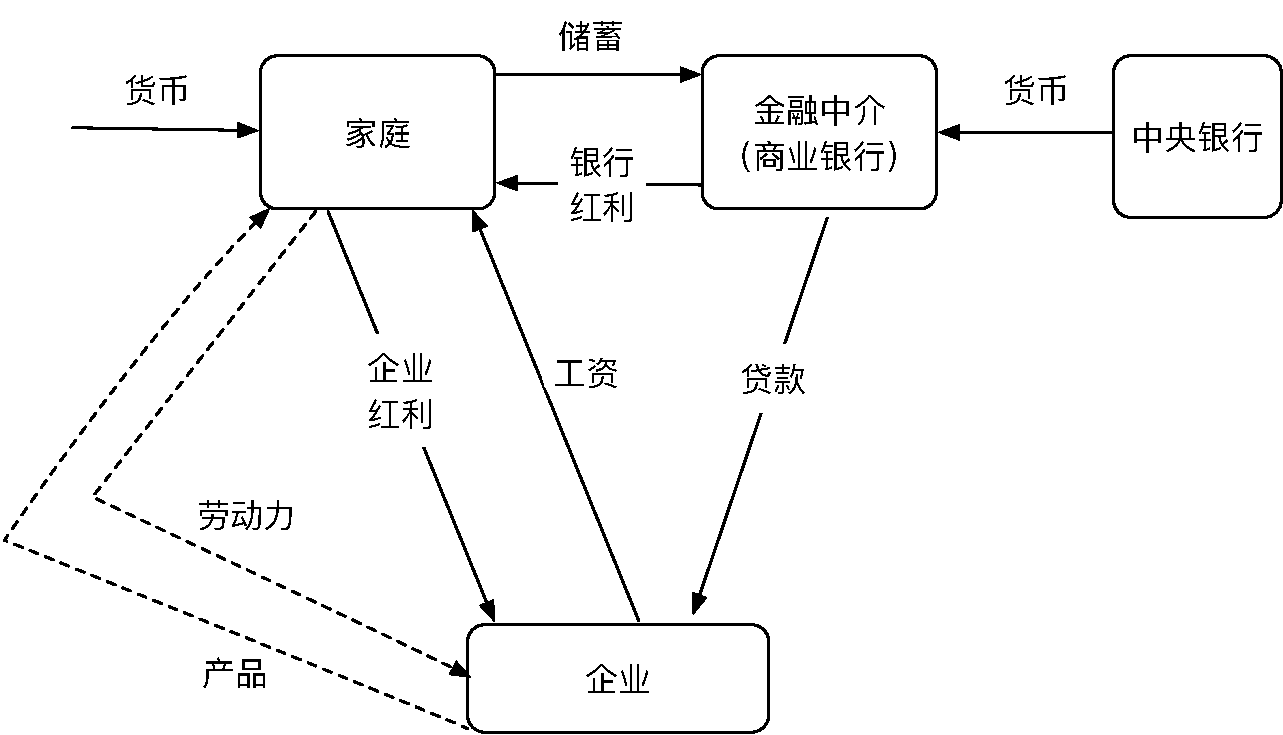
\includegraphics[width=4in]{./figures/20170324-CIA-outline}
 \caption{CIA DSGE模型结构图}
\label{fig:CIA-blueprint}

  \small{注:实线表示名义资金流动。虚线表示实际物质流动。}
\end{figure}

\section{家庭部门}
假定一个永生家庭,追求期望效用的最大化
\begin{equation}
  \label{eq:CIA-hh-max-util}
  \max%_{C_t,H_t,D_t,M_{t+1}}
  E_0 \sum_{t=0}^{\infty} \beta^t \left[ (1-\phi) \cdot \ln C_t + \phi \cdot \ln (1-H_t)\right].
\end{equation}
其中变量$ C_t$表示消费,$0<H_t<1$ 表示劳动时间占全部可支配时间的比重。系数$0<\beta<1$表示时间折旧,$0< \phi <1$表示消费$C_t$相对于休闲$(1-H_t)$,对效用的重要程度。

家庭效用最大化受到2+1个条件限制。

第1个是家庭的现金平衡条件,假定$t$时期家庭需要存留足够数量的现金,以满足同期全部消费需求:
\begin{equation}
  \label{eq:CIA-hh-cash-balance}
  W_t \cdot H_t + M_t - D(t) \ge P_t \cdot C_t,
\end{equation}
其中等式左侧$W_t$表示由市场给定的劳动力平均工资,%$N_t$表示企业部门的劳动力需求,
$M_t$表示$t-1$期末经济体中的基础货币存量,$D_t$表示家庭部门的储蓄,假定储蓄全部以存款形式$D_t$存入银行部门,$M_t$。等式右侧$P_t$表示市场给定的最终产品价格。cash balance是CIA-DSGE模型的核心设定之一。

第2个是家庭的资源约束条件
\begin{equation}
  \label{eq:CIA-hh-rsource-constraint}
  M_{t+1} \ge \left(M_t - D_t + W_t \cdot H_t - P_t \cdot C_t\right) + R_{H,t} \cdot D_t + \left(F_t + B_t\right),
\end{equation}
%等式左侧表示$t$期末经济体中的基础货币存量;
等式右侧分为三个部分。第一部分为现金平衡条件如式\eqref{eq:CIA-hh-cash-balance},第二部分为家庭存款$D_t$的收益,$R_{H,t}$为银行提供给家庭的无风险名义存款利率,第三部分为家庭部门收到的分红\footnote{模型假定银行和企业的资产最终由家庭部门所有,如\cite{Christiano:1992fz}。},分别来自银行部门$B_t$和企业部门$F_t$。根据资源约束条件,$t$期家庭需要决定全部收入中提取多少现金存留在手上,以满足$t$期的消费需求;剩余部分以$D_t$形式存入银行,获取利润,以供$t+1$期消费所用。

第3个是家庭净资产非负条件,假定所有时期家庭的储蓄均大于$0$
\begin{equation}
  \label{eq:CIA-hh-non-negative-deposits-constraint}
  D_t \ge 0.
\end{equation}

\section{企业部门}
假定完全竞争市场环境下,一家典型企业的生产函数
\begin{equation}
  \label{eq:CIA-firm-production-function}
  Y_t = K_t^{\alpha} \cdot (A_t \cdot N_t)^{1-\alpha},
\end{equation}
符合Cobb-Douglas形式。投入要素有2。第1个投入要素为资本存量$K_t$,通过企业往期投资$I_{t-s}, s>0$,经折旧后累积形成,
\begin{equation}
  \label{eq:CIA-firm-capital-accumulation}
  K_{t+1} = I_{t} + (1-\delta) \cdot K_t,
\end{equation}
其中常系数$0<\delta<1$表示自然折旧率。

第2个投入要素为劳动力$N_t$。基于市场给定的名义工资率$W_t$,企业向银行借贷$L_t$,用于支付全部劳动工资
\begin{equation}
  \label{eq:CIA-firm-lending-balance}
  L_t \ge W_t \cdot N_t,
\end{equation}
银行借贷需要支付市场利率$R_{F,t}$。

此外式\eqref{eq:CIA-firm-production-function}中,$\alpha$表示资本的产出弹性。外生变量$A_t$用于描述劳动扩张型技术进步,见第\ref{sec:CIA-exo-shocks}节。

\subsection{生产规模}
如前文所述,完全竞争市场下,利润最大化企业以$R_{F,t}$利率从银行获取贷款$L_t$用于成本支出,即支付员工工资$W_t \cdot N_t$,展开生产。企业将逐渐增加生产规模,直到雇佣额外1单位劳动力的边际收益,等于向银行借贷所需支付的利息。

\begin{equation}
  \label{CIA-firm-optim-partial}
  \frac{\partial \left[ P_t \cdot Y_t - W_t \cdot N_t \right]}{\partial N_t} + \frac{\partial \left[ (1-R_{F,t}) \cdot L_t \right]}{\partial N_t} = 0.
\end{equation}

%设企业追求利润最大化\todo{利润生产和利润使用。利润生产方面,需要补上一段。}。

\subsection{利润的使用}
对于已经生成的利润,$t$期企业核心决策为,决定利润中多少比例留作投资$I_t$,以增加$t+1$期的资本存量$K_{t+1}$,用于扩大再生产;剩余利润以红利$F_t$形式返回家庭部门,用于$t+1$期的消费$C_{t+1}$。企业行为可以表示如下
\begin{equation}
  \label{CIA-firm-max-problem}
  \max E_0 \sum_{t=0}^{\infty} \beta^{t+1} \cdot \frac{F_t}{P_{t+1} \cdot C_{t+1}}.
\end{equation}

企业利润最大化生产活动受到2个条件限制。第1个是预算约束条件,
\begin{equation}
  \label{eq:CIA-firm-budget-constraint}
  P_t \cdot (Y_t-I_t) + L_t \ge F_t + W_t \cdot N_t + R_{F,t} \cdot L_t,
\end{equation}
等式右侧表示全部生产收入和来自银行的贷款;左侧支出部分分别为给家庭部门的红利,劳动力工资,和向银行支付的贷款利息。

第2个是非负借贷条件式\eqref{eq:CIA-firm-lending-balance},确保当期向银行借款数足以支付工资。

\section{银行部门}
类似地,$t$期的银行利润以分红$B_t$形式返还给家庭部门,用于$t+1$期的消费。利润最大化的银行追求
\begin{equation}
  \label{eq:CIA-bank-max-problem}
  \max E_t \sum_{t=0}^{\infty} \beta^{t+1} \cdot \frac{B_{t}}{P_{t+1} \cdot C_{t+1}}.
\end{equation}

银行利润最大化行为受到2个条件限制。第1个是预算约束条件
\begin{equation}
  \label{eq:CIA-bank-budget-constraint}
  B_t + R_{H,t} \cdot D_t \le R_{F,t} \cdot L_t + D_t + X_t - L_t,
\end{equation}
其中$X_t$表示$t$期中央银行对市场释放的基础货币,定义为$t+1$期末基础货币存量和$t$期末基础货币存量的差,
\begin{equation}
  \label{eq:CIA-central-bank-money-injection}
  X_t = M_{t+1} - M_t.
\end{equation}

第2个是资产负债平衡约束,要求同期的银行负债不得超过资产
\begin{equation}
  \label{eq:CIA-bank-balance-sheet}
  X_t + D_t \le L_t.
\end{equation}

\section{一阶条件}
\subsection{家庭部门}
根据最大化式\eqref{eq:CIA-hh-max-util}及约束条件式\eqref{eq:CIA-hh-cash-balance}-\eqref{eq:CIA-hh-non-negative-deposits-constraint},建家庭部门Lagrangian

\begin{align*}
  \mathcal{L} = E_0 \sum_{t=0}^{\infty} \beta^t \cdot & \left\{
\left[(1-\phi) \cdot \ln C_t + \phi \cdot \ln (1-H_t)\right]
   \right. \\
   & \left. + \lambda_t \cdot
   \left[
M_t - D_t + W_t \cdot H_t - P_t \cdot C_t + R_{H,t} \cdot D_t + \left( F_t + B_t - M_{t+1} \right)
   \right]\right\}.
\end{align*}

FOCs:
\begin{align}
  \label{eq:CIA-hh-FOC-C}
  \frac{\partial \mathcal{L}}{\partial C_t} = 0 &\Rightarrow \lambda_t = \frac{1-\phi}{P_t \cdot C_t}, \\
  \label{eq:CIA-hh-FOC-H}
  \frac{\partial \mathcal{L}}{H_t}=0 &\Rightarrow \lambda_t \cdot W_t = \frac{\phi}{1-H_t},\\
  \label{eq:CIA-hh-FOC-M}
  \frac{\partial \mathcal{L}}{\partial M_{t+1}} = 0 &\Rightarrow \frac{\partial \beta \cdot E_t \cdot \left( \lambda_{t+1} \cdot R_{H,t+1} \cdot D_{t+1} \right)}{\partial M_{t+1}} = \lambda_t.
\end{align}

\subsection{企业部门}
利用
将式\eqref{eq:CIA-firm-capital-accumulation}、\eqref{eq:CIA-firm-production-function}
代入\eqref{eq:CIA-firm-budget-constraint}替换$I_t$、$Y_t$,与式  \eqref{eq:CIA-firm-lending-balance}共同构成约束条件
\begin{equation*}
  P_t \cdot \left[
K_t^{\alpha} \cdot \left(A_t \cdot N_t \right)^{1-\alpha} - K_{t+1} + (1-\delta) \cdot K_t
  \right] \ge F_t + W_t \cdot N_t + R_{F,t} \cdot L_t - L_t.
\end{equation*}

建企业部门Lagrangian
\begin{align*}
  \mathcal{L} = E_t \sum_{t=0}^{\infty} \beta^{t+1} \cdot &\left\{ \frac{F_t}{P_{t+1} \cdot C_{t+1}} \right. \\
  &+\left. \lambda_t \cdot \left\{
P_t \cdot \left[ K_t^{\alpha} \cdot \left( A_t \cdot N_t \right)^{1-\alpha} - K_{t+1} + (1-\delta) \cdot K_t \right] - F_t - W_t \cdot N_t - R_{F,t} \cdot L_t + L_t
  \right\} \right\}.
\end{align*}

FOCs:
\begin{align}
  \label{eq:CIA-firm-FOC-F}
  \frac{\partial \mathcal{L}}{\partial F_t} = 0 & \Rightarrow \lambda_t = E_t \frac{1}{P_{t+1} \cdot C_{t+1}}, \\
  \label{eq:CIA-firm-FOC-N}
  \frac{\partial \mathcal{L}}{\partial N_t} = 0 & \Rightarrow P_t \cdot K_{t}^{\alpha} \cdot (1-\alpha) \cdot A_t^{1-\alpha} \cdot N_t^{-\alpha} = W_t,\\
  \label{eq:CIA-firm-FOC-K}
  \frac{\partial \mathcal{L}}{\partial K_{t+1}} = 0 &\Rightarrow \lambda_t \cdot P_t = \beta \cdot E_t \lambda_{t+1} \cdot P_{t+1} \cdot \left[
\alpha \cdot K_{t+1}^{\alpha - 1} \cdot \left( A_{t+1} \cdot N_{t+1} \right)^{1-\alpha} + (1-\delta)
  \right].
\end{align}

\subsection{银行部门}
建立银行部门Lagrangian

\begin{align*}
  \mathcal{L} = E_t \sum_{t=0}^{\infty} \beta^{t+1} \cdot & \left\{ \frac{B_t}{P_{t+1} \cdot C_{t+1}} \right. \\
  &\left.
  + \lambda_t \cdot \left(D_t + R_{F,t} \cdot L_t - R_{H,t} \cdot D_t - L_t + X_t - B_t \right)
  \right\}.
\end{align*}

\subsection{一阶条件的整理}
式\eqref{eq:CIA-hh-FOC-C}代入式\eqref{eq:CIA-hh-FOC-H}以替换$\lambda_t$,可得劳动力供应的决定式
\begin{equation}
  \label{eq:CIA-FOC-labor-supply}
  W_t = \frac{\phi}{1-\phi} \cdot \frac{P_t \cdot C_t}{1-H_t}.
\end{equation}

式\eqref{eq:CIA-hh-FOC-C}代入式\eqref{eq:CIA-hh-FOC-M}以替换$\lambda_t$;结合式\eqref{eq:CIA-bank-budget-constraint}、\eqref{eq:CIA-central-bank-money-injection}可得跨期消费的Euler equation
\begin{equation}
  \label{eq:CIA-FOC-intertemp-consumption-euler}
  \frac{1}{P_t \cdot C_t} = R_{H,t} \cdot \beta \cdot E_t \frac{1}{P_{t+1} \cdot C_{t+1}}.
\end{equation}

\eqref{eq:CIA-firm-FOC-F}代入式\eqref{eq:CIA-firm-FOC-N}以替换$\lambda_t$,可得劳动力需求的决定式
\begin{equation}
  \label{eq:CIA-FOC-labor-demand}
  W_t = \left( 1-\alpha \right) \cdot P_t \cdot K_t^{\alpha} \cdot A_{t}^{1- \alpha} \cdot N_t^{-\alpha}.
\end{equation}

 \eqref{eq:CIA-firm-FOC-F}代入式\eqref{eq:CIA-firm-FOC-K}以替换$\lambda_t$,可得产品市场上跨期消费决策的Euler equation
\begin{equation}
  \label{eq:CIA-FOC-goods}
  E_t \frac{P_t}{P_{t+1} \cdot C_{t+1}} = \beta \cdot E_t \cdot
  \left\{
\left( \frac{P_{t+1}}{P_{t+2} \cdot C_{t+2}} \right) \cdot
\left[
  \alpha \cdot K_{t+1}^{\alpha -1 } \cdot
  \left(A_{t+1} \cdot N_{t+1} \right)^{1-\alpha} + (1-\delta)
\right]
  \right\}.
\end{equation}


\section{市场均衡及部门最优行为}

\subsection{4个市场均衡条件}
假定下述4个完全竞争市场均处于均衡条件,完全出清。

\subsubsection{劳动力市场均衡}

家庭部门的劳动力供应等于企业部门的劳动力需求
\begin{equation}
  \label{eq:CIA-market-clearing-labor}
  H_t = N_t.
\end{equation}

\subsubsection{产品市场均衡}

企业部门的产出完全用于企业再投资和家庭部门的消费
\begin{equation}
  \label{eq:CIA-market-clearing-product}
  Y_t = C_t + I_t.
\end{equation}

\subsubsection{货币市场均衡}

家庭部门对现金(消费)的需求,等于市场上的货币供应
\begin{equation}
  \label{eq:CIA-market-clearing-money}
  P_t \cdot C_t = M_{t+1}.
\end{equation}

\subsubsection{信贷市场均衡}

商业银行的负债等于资产,即式\eqref{eq:CIA-bank-balance-sheet}改写为
\begin{equation}
  \label{eq:CIA-market-clearning-credit}
  X_t + D_t = L_t.
\end{equation}



\subsection{部门最优行为}
将几个市场的均衡行为纳入部门最优行为的决策分析。

\subsubsection{劳动力市场}
劳动力市场均衡条件下,式\eqref{eq:CIA-firm-lending-balance}取等号,可求得平均工资的决定
\begin{equation}
  \label{eq:CIA-wage-determ}
  W_t = \frac{L_t}{N_t}.
\end{equation}

将劳动力市场出清式\eqref{eq:CIA-market-clearing-labor}和均衡工资决定式\eqref{eq:CIA-wage-determ}代入一阶条件式\eqref{eq:CIA-FOC-labor-supply},分别替代$W_t, H_t$可得家庭部门的同期最优消费——劳动供应决策。
\begin{equation}
  \label{CIA-optimal-labor-mkt-intratemp}
  \frac{L_t}{N_t}=\frac{\phi}{1-\phi} \cdot \frac{P_t \cdot C_t}{1-N_t}.
\end{equation}

\subsubsection{产品市场}
产品市场最优条件,见跨期消费平滑Euler equation式\eqref{eq:CIA-FOC-goods}。

\subsubsection{货币市场}
式\eqref{eq:CIA-central-bank-money-injection}代入货币市场均衡条件式\eqref{eq:CIA-market-clearing-money}可得
\begin{equation}
  \label{eq:CIA-market-clearing-money-flow}
  P_t \cdot C_t = M_t + X_t,
\end{equation}
即全部现金需求等于市场上的货币存量和当期新增货币投放量之和。

\subsubsection{信贷市场}
首先由信贷市场均衡式\eqref{eq:CIA-market-clearning-credit}可见,根据银行利润为零的假定
\begin{equation*}
  R_{H,t} \cdot D_t = R_{F,t} \cdot \left(L_t - X_t \right),
\end{equation*}
由此我们有
\begin{equation}
  \label{eq:CIA-interest-rate-unification}
  R_{F,t} = R_{H,t} \equiv R_t.
\end{equation}

式\eqref{eq:CIA-firm-production-function}、\eqref{eq:CIA-wage-determ}和
\eqref{eq:CIA-interest-rate-unification} 代入式\eqref{CIA-firm-optim-partial}分别替换$Y_t, L_t, R_{F,t}$,整理后,可得信贷市场最优条件
\begin{equation}
  \label{CIA-optimal-credit-mkt}
  R_t = \frac{P_t \cdot K_t^{\alpha} \cdot (1-\alpha) \cdot A_t^{1- \alpha} \cdot N_t^{-\alpha}}{W_t}.
\end{equation}

\section{外生冲击}
\label{sec:CIA-exo-shocks}
经济模型中存在两种随机外生冲击。第1种是作用于实体经济部门的劳动增强型技术冲击,假定符合下述形式
\begin{equation}
  \label{eq:CIA-tech-shock}
  \ln A_t = \gamma + \ln A_{t-1} + \varepsilon_{A,t}, \quad \varepsilon_{A,t} \sim \mathcal{N}(0,\sigma_A^2), \quad corr(\varepsilon_{A,t}, \varepsilon_{A,s})=0, \forall s \neq t,
\end{equation}
$\gamma > 0$表示确定性趋势。不可提前预支的当期技术波动用innovation项$\varepsilon_{A,t}$来反映。

由定义式\eqref{eq:CIA-tech-shock}可得外生技术冲击的增速
\begin{equation}
  \label{eq:CIA-tech-shock-growth}
  \frac{A_t}{A_{t-1}} = \exp (\gamma + \varepsilon_{A,t}).
\end{equation}

第2种是作用于非实体非实体经济部门的货币投放增速的冲击。假定货币投放增速表述为
\begin{equation}
  \label{eq:CIA-money-injection-growth-def}
  m_t \equiv \frac{M_{t+1}}{M_t},
\end{equation}
随机冲击符合下述形式
\begin{equation}
  \label{eq:CIA-money-shock}
  \ln m_t = (1-\rho) \cdot \ln m^{*} + \rho \cdot \ln m_{t-1} + \varepsilon_{m,t}, \quad \varepsilon_{m,t} \sim \mathcal{N}(0,\sigma_m^2),  \quad corr(\varepsilon_{m,t}, \varepsilon_{m,s})=0, \forall s \neq t.
\end{equation}
$m^{*}$表示$m_t$的无条件均值。$m^{*}$和$0<\rho<1$一道用于描述常规货币政策,进而二者的变化反映了货币政策的调整。模型引入随机innovation $\varepsilon_{m,t}$表示当期影响货币供应增速变化的波动因素\citep{Sims:1982ks}。

\section{均衡方程组}
\label{sec:CIA-equilibrium-conditions}
模型均衡方程组由9个内生变量和2个外生变量$\{K_{t+1}, N_t, D_t, C_t, L_t, P_t, W_t, Y_t, R_t, A_t/A_{t-1}, m_t\}$共同构成\footnote{有的时候还需要考虑一个派生变量,通货膨胀$\pi_t = \frac{P_t}{P_{t-1}}$。}。对应一组结构方程如下,每个方程的经济学含义在第\ref{sec:CIA-scaling-equilibrium-conditions}节做简要描述:

式\eqref{eq:CIA-wage-determ}、\eqref{CIA-optimal-credit-mkt}代入\eqref{CIA-optimal-credit-mkt}以替代$W_t,R_t$得
  \begin{equation}
    \label{eq:CIA-equil-cond-unscal-inter-euler}
    \frac{1}{P_t \cdot C_t} = \frac{\beta \cdot P_t \cdot K_t^{\alpha} \cdot (1-\alpha) \cdot A_{t}^{1-\alpha} \cdot N_t^{1-\alpha}}{L_t \cdot E_t P_{t+1} \cdot C_{t+1}}.
  \end{equation}

式\eqref{eq:CIA-FOC-goods} $\Rightarrow$
  \begin{equation*}
    E_t \frac{P_t}{P_{t+1} \cdot C_{t+1}} = \beta \cdot E_t \cdot
    \left\{
  \left( \frac{P_{t+1}}{P_{t+2} \cdot C_{t+2}} \right) \cdot
  \left[
    \alpha \cdot K_{t+1}^{\alpha -1} \cdot
    \left(A_{t+1} \cdot N_{t+1} \right)^{1-\alpha} + (1-\delta)
  \right]
    \right\}.
  \end{equation*}

式\eqref{CIA-optimal-labor-mkt-intratemp} $\Rightarrow$
  \begin{equation*}
    \frac{L_t}{N_t}=\frac{\phi}{1-\phi} \cdot \frac{P_t \cdot C_t}{1-N_t}.
  \end{equation*}

式\eqref{eq:CIA-firm-capital-accumulation}、\eqref{eq:CIA-firm-production-function}代入式\eqref{eq:CIA-market-clearing-product}以替换$I_t, Y_t$ $\Rightarrow$
    \begin{equation}
    \label{eq:CIA-equil-cond-unscal-resource}
      K_t^{\alpha} \cdot \left( A_t \cdot N_t \right)^{1-\alpha} = C_t + K_{t+1} - \left( 1 - \delta \right) \cdot K_t.
    \end{equation}

式\eqref{eq:CIA-market-clearing-money} $\Rightarrow$
  \begin{equation*}
    P_t \cdot C_t = M_{t+1}.
  \end{equation*}

式\eqref{eq:CIA-central-bank-money-injection}代入\eqref{eq:CIA-market-clearning-credit}以替代$X_t$ $\Rightarrow$
  \begin{equation}
    \label{eq:CIA-equil-cond-unscal-credit}
    L_t = D_t + M_{t+1} - M_{t}.
  \end{equation}

式\eqref{eq:CIA-firm-production-function} $\Rightarrow$
  \begin{equation*}
    Y_t = K_t^{\alpha} \cdot (A_t \cdot N_t)^{1-\alpha},
  \end{equation*}

式\eqref{eq:CIA-wage-determ} $\Rightarrow$
  \begin{equation*}
    W_t = \frac{L_t}{N_t}.
  \end{equation*}

式\eqref{CIA-optimal-credit-mkt} $\Rightarrow$
  \begin{equation*}
    R_t = \frac{P_t \cdot K_t^{\alpha} \cdot (1-\alpha) \cdot A_t^{1- \alpha} \cdot N_t^{-\alpha}}{W_t}.
  \end{equation*}

外生冲击式\eqref{eq:CIA-tech-shock} $\Rightarrow$
  \begin{equation*}
    \ln A_t = \gamma + \ln A_{t-1} + \varepsilon_{A,t}, \quad \varepsilon_{A,t} \sim \mathcal{N}(0,\sigma_A^2), \quad corr(\varepsilon_{A,t}, \varepsilon_{A,s})=0, \forall s \neq t,
  \end{equation*}

外生冲击式\eqref{eq:CIA-money-shock} $\Rightarrow$
  \begin{equation*}
    \ln m_t = (1-\rho) \cdot \ln m^{*} + \rho \cdot \ln m_{t-1} + \varepsilon_{m,t}, \quad \varepsilon_{m,t} \sim \mathcal{N}(0,\sigma_m^2),  \quad corr(\varepsilon_{m,t}, \varepsilon_{m,s})=0, \forall s \neq t.
  \end{equation*}


\section{去趋势的均衡状态}
\label{sec:CIA-scaling-equilibrium-conditions}
第\ref{sec:CIA-equilibrium-conditions}节的方程组是非平稳的。非平稳来自两方面因素,第一是随机技术冲击和货币冲击的趋势影响。即便假定冲击均为零,第二方面因素在于各变量之间没有统一的稳定状态:实际变量的增速等于$A_t$的增速(除了劳动力$N_t$);名义变量的增速等于$M_t$的增速;总物价水平的增速等于$M_t/A_t$的增速。对上节的变量做去趋势调整:
\begin{equation*}
\begin{cases}
  \text{(名义变量)}&\hat{\mathcal{B}}_t=\frac{\mathcal{B}_t}{A_t} \text{, 其中 } \mathcal{B}_t=[Y_t,C_t,I_t,K_{t+1}]',\\
  \text{(实际变量)}&\hat{\mathcal{C}}_t = \frac{\mathcal{C}_t}{M_t} \text{, 其中 } \mathcal{C}_t=[W_t,D_t,L_t]', \\
  \text{(名义变量)}&\hat{P}_t = \frac{P_t \cdot A_t}{M_t},\\
  \text{(其他)}&\{N_t, R_t\}\text{保持不变,根据式}  \eqref{eq:CIA-money-injection-growth-def}\text{用$m_t - 1$替代$\frac{X_t}{M_t}$}.
\end{cases}
\end{equation*}

由去趋势变量构成的新方程组如下。

式\eqref{eq:CIA-equil-cond-unscal-inter-euler} $\Rightarrow$
\begin{align}
  \frac{1}{\left(\frac{\hat{P}_t \cdot M_{t}}{A_t}\right) \cdot \left(\hat{C}_t \cdot A_t \right)} &=
  \frac{
  \beta \cdot \left(\frac{\hat{P}_t \cdot M_t}{A_t}\right) \cdot \left(\hat{K}_t^{\alpha} \cdot A_{t-1}^{\alpha} \right) \cdot (1-\alpha) \cdot A_t^{1-\alpha} \cdot N_t^{1-\alpha}
  }{
  \left(\hat{L}_t \cdot M_t \right) \cdot E_t \cdot \left(\frac{\hat{P}_{t+1} \cdot M_{t+1}}{A_{t+1}}\right) \cdot \left( \hat{C}_{t+1} \cdot A_{t+1} \right)
  },
  \nonumber \\
  \frac{1}{\hat{P}_t \cdot \hat{C}_t \cdot M_t} &= \frac{
  (1-\alpha) \cdot \beta \cdot \hat{P}_t \cdot M_t \cdot \hat{K}_t^{\alpha} \cdot N_t^{1-\alpha} \cdot \left(\frac{A_t}{A_{t-1}}\right)^{-\alpha}
  }{
  \left(\hat{L}_t \cdot M_t\right) \cdot E_t M_{t+1} \cdot \hat{P}_{t+1} \cdot \hat{C}_{t+1}
  },\nonumber \\
  \label{eq:CIA-equil-cond-scal-inter-euler}
  \frac{1}{\hat{P}_t \cdot \hat{C}_t} &=  \frac{
  (1-\alpha)\cdot \beta \cdot \frac{\hat{P}_t \cdot \hat{K}_t^{\alpha} \cdot N_t^{1-\alpha}}{\hat{L}_t \cdot m_t} \cdot \exp \left[ - \alpha \cdot \left( \gamma + \varepsilon_{A,t} \right)\right]
  }{
  E_t \hat{P}_{t+1} \cdot \hat{C}_{t+1}
  }.
\end{align}
反映信贷市场的最优跨期决策,使得今天放弃1单位消费用于储蓄,导致明天消费增加的现值,等于今天1单位消费带来的满足。

式\eqref{eq:CIA-FOC-goods} $\Rightarrow$
\begin{equation*}
  \frac{P_t}{E_t P_{t+1}\cdot C_{t+1}}
  = \frac{
  \frac{\hat{P}_t \cdot M_t }{A_t}
  }{
  E_t \left(
   \frac{\hat{P}_{t+1} \cdot \hat{M}_{t+1}}{A_{t+1}}
  \right) \cdot \left(
  \hat{C}_{t+1} \cdot A_{t+1}
  \right)
  }
  =\frac{\hat{P}_t}{E_t \hat{P}_{t+1} \cdot \hat{C}_{t+1} \cdot m_t \cdot A_t}
\end{equation*}
进而我们有
\begin{equation*}
  E_t \frac{\hat{P}_t}{\hat{P}_{t+1} \cdot \hat{C}_{t+1} \cdot m_t} = \beta \cdot E_t \frac{\hat{P}_{t+1}}{\hat{P}_{t+2} \cdot \hat{C}_{t+2} \cdot m_{t+1} \cdot \left(\frac{A_{t+1}}{A_t}\right)} \cdot \left[
  \alpha \cdot \hat{K}_{t+1}^{\alpha-1} \cdot N_{t+1}^{1-\alpha} \cdot
  \left(\frac{A_{t+1}}{A_t}\right)^{1-\alpha} + \left( 1-\delta \right)
  \right],
\end{equation*}
\begin{align}
  \label{eq:CIA-FOC-goods-scal}
 E_t \frac{\hat{P}_t}{\hat{P}_{t+1} \cdot \hat{C}_{t+1} \cdot m_t} = \beta \cdot E_t \frac{
 \hat{P}_{t+1}
 }{
 \hat{P}_{t+2} \cdot \hat{C}_{t+2} \cdot m_{t+1}
 } \cdot & \left\{
\alpha \cdot \hat{K}_{t+1}^{\alpha -1} \cdot N_{t+1}^{ 1-\alpha} \cdot \exp \left[-\alpha \cdot \left(\gamma + \varepsilon_{A,t+1}\right)\right] \right.\nonumber \\
& \left. + \left( 1-\delta \right) \cdot \exp \left[ -1 \cdot \left( \gamma + \varepsilon_{A,t+1} \right) \right] \right\}.
\end{align}
反映产品市场的跨期最优决策,确保经济体整体的跨期消费平滑。

式\eqref{CIA-optimal-labor-mkt-intratemp} $\Rightarrow$
\begin{equation}
  \label{CIA-optimal-labor-mkt-intratemp-scal}
  \frac{\hat{L}_t}{N_t}=\frac{\phi}{1-\phi} \cdot \frac{\hat{P}_t \cdot \hat{C}_t}{1-N_t}.
\end{equation}
反映劳动力市场的当期最优决策:家庭部门的劳动力供应(企业部门的劳动力需求),和消费——休闲边际替代率之间的关系。

式\eqref{eq:CIA-equil-cond-unscal-resource} $\Rightarrow$
\begin{equation}
  \label{eq:CIA-equil-cond-scal-resource}
  \hat{K}_t^{\alpha} \cdot N_t^{1-\alpha} \cdot \exp \left[ -\alpha \cdot \left( \gamma + \varepsilon_{A,t} \right) \right] = \hat{C}_t + \hat{K}_{t+1} -  (1-\delta) \cdot \hat{K}_t \cdot \exp \left[
  -1 \cdot \left( \gamma + \varepsilon_{A,t} \right)
  \right].
\end{equation}
反映总量上的资源约束条件:当期产出全部用于当期消费和当期投资;当期投资贡献于下一期的资本存量积累。

式\eqref{eq:CIA-market-clearing-money} $\Rightarrow$
\begin{equation}
  \label{eq:CIA-market-clearing-money-scal}
  \hat{P}_t \cdot \hat{C}_t = m_t.
\end{equation}
反映货币市场的最优决策:货币的名义消费需求等于名义货币供应量。名义货币供应量等于名义现有货币存量与当期货币注入量之和。

式\eqref{eq:CIA-equil-cond-unscal-credit} $\Rightarrow$
\begin{equation}
  \label{eq:CIA-equil-cond-scal-credit}
  \hat{L}_t = \left( m_t - 1 \right) + \hat{D}_t.
\end{equation}
反映信贷市场的最优决策:商业银行追求资产——负债平衡。

式\eqref{eq:CIA-firm-production-function} $\Rightarrow$
\begin{equation}
  \label{eq:CIA-firm-production-function-scal}
  \hat{Y}_t = \hat{K}_t^{\alpha} \cdot N_t^{1-\alpha} \cdot \exp \left[ - \alpha \cdot \left( \gamma + \varepsilon_{A,t} \right) \right].
\end{equation}
反映经济整体的投入产出关系。

式\eqref{eq:CIA-wage-determ} $\Rightarrow$
\begin{equation}
  \label{eq:CIA-wage-determ-scal}
  \hat{W}_t = \frac{\hat{L}_t}{N_t}.
\end{equation}
反映企业对商业银行的贷款需求,与企业生产活动中的劳动力需求(家庭部门的劳动力供应)之间的关系。

式\eqref{CIA-optimal-credit-mkt} $\Rightarrow$
\begin{equation}
  \label{CIA-optimal-credit-mkt-scal}
  R_t = \left( 1-\alpha \right) \cdot \frac{\hat{P}_t \cdot \hat{K}_t^{\alpha} \cdot N_t^{1 - \alpha}}{\hat{L}_t} \cdot \exp \left[ -\alpha \cdot \left( \gamma + \varepsilon_{A,t} \right) \right].
\end{equation}
反映信贷市场的最优决策:均衡利率水平表示额外1单位劳动力投入的边际产出效果,等于借贷用于雇佣此额外1单位劳动力所需支付的成本。

外生技术冲击和货币冲击,如式\eqref{eq:CIA-tech-shock-growth}、\eqref{eq:CIA-money-shock}所示。

此外,实际观测到的经济增速和稳定状态下的经济增速之间的关系如下
\begin{equation}
  \label{eq:CIA-gdp-growth-obs-stab}
  \frac{Y_t}{Y_{t-1}}=\frac{\hat{Y}_t}{\hat{Y}_{t-1}} \cdot \exp \left( \gamma + \varepsilon_{A,t} \right).
\end{equation}

类似地,实际观测到的通货膨胀和稳定状态下的通货膨胀之间关系如下
\begin{equation}
  \label{eq:CIA-inflation-obs-stab}
  \frac{P_t}{P_{t-1}} = \frac{\hat{P}_{t}}{\hat{P}_{t-1}} \cdot m_{t-1} \cdot \exp \left[ -1 \cdot \left( \gamma + \varepsilon_{A,t} \right) \right]
\end{equation}




\part{模型求解}
%!TEX root = ../DSGEnotes.tex
\chapter{DSGE模型求解方法简论}
\label{sec:solution-strat}


\section{简论的简论}
过去的三十多年来,宏观经济学研究经历了一场飞速变革。这场变革始于\cite{Kydland:1982cd}利用RBC模型研究美国经济。这种研究方法逐渐成为宏观经济学的标准范式之一\citep{An:2007cv, FernandezVillaverde:2010fq}。

随后RBC模型逐渐扩展到新凯恩斯主义模型。经典教材如\cite{Gali:2005gp,Woodford:2011ks}。然而新凯恩斯主义模型也远非完美无缺,随着新的问题逐渐被发现,学术界对模型做了进一步的修正和扩展,使模型对现实的拟合程度越来越高,如
\begin{itemize}
  \item 根据基准黏性价格假定所生成的一些重要经济变量的时间序列,与实际观察到的经济现实相比,出入较大——真实经济世界中的通货膨胀,产出,实际工资等时间序列数据都具有很高的持续性——为了使得模型与现实相贴近,模型设定中就需要引入看起来异常高的名义粘性。
  \item 因此产生了一系列对基准新凯恩斯模型的扩展,它们的基本思路是,加入\cite{Calvo:1983uq} 定价机制,从而可以在控制名义粘性不至于过高的情况下,有效提高模型生成的通货膨胀时间序列数据的持续性 \citep{Rabanal:2005ii}。
\end{itemize}

这样新凯恩斯主义分析框架得到了中央银行等政策制定者的青睐。不同中央银行开发了一系列自己的DSGE模型,如
\begin{itemize}
  \item 欧洲中央银行(ECB)的NAWM (New Ara-Wide Model)。

  在\cite{Fagan:2005hv}的Area-Wide Model (ARM)和\cite{Smets:2003ic}的基础上,\cite{Christoffel:2008vq} 开发了欧元区的NAWM,一个基于微观经济基础的开放经济模型,广泛应用于欧洲中央银行研究人员对经济系统的预测。
  \item 加拿大银行 (Bank of Canada)的ToTEM (Term-of-Trade Economic Model),见\cite{Murchison:2006wc}。
  \item 英格兰银行 (Bank of England)的BEQM (Bank of England Quarterly Model),见\cite{Harrison:2005tc}。
  \item 挪威银行 (Norges Bank)的NEMO (Norwegian Economy Model),见\cite{Brubakk:2006vu}。
  \item 智利中央银行(Central Bank of Chile)的MAS (Model of Analysis and Simulation), 见\cite{Medina:2007tz}。
  \item 瑞典中央银行 (Sveriges Riksbank)的RAMSES (Riksbanks Aggregated Model for Studies of the Economy in Sweden),见\cite{Adolfson:2007bv,Adolfson:2008cs}。
  \item 美联储的SIGMA。

  在\cite{Obstfeld:1995jp}的开放经济体模型基础上,\cite{Erceg:2006tf}简历的多国家开放经济模型。
  \item 国际货币基金组织(IMF)的GEM (Global Economic Model),见\cite{Bayoumi:2004vx}。
\end{itemize}

上述中央银行开发的经济预测模型,多得以于DSGE模型的长处,具有如下特征:
\begin{enumerate}
  \item 动态性。关注变量岁时间的变化路径,而不是某单独时间点上的情况。
  \item 整体性。致力于解释、预测整体经济运行,而非仅仅是局部市场。

  但这并不意味着DSGE模型可以重现整个经济系统的没一个重要部分,尤其是其中一些部门常常需要做必要的简化处理,如财政政策的制定部门(政府)、金融市场等。
  \item 重视部门均衡。根据经济学理论,在不同市场中,重视市场调节机制作用下的供应需求平衡。
  \item 模型中引入随机干扰。
\end{enumerate}

从广义的宏观经济学模型角度来看,DSGE模型可以分为两大类:RBC模型和新凯恩斯主义模型。RBC模型致力于研究在灵活价格环境下的经济周期波动,常表现为两部分的组合:一部分是随机内生经济增长模型作为内核,另一部分是外部真实技术冲击。\cite{Kydland:1982cd} 对RBC模型(进而DSGE模型)研究做出了开创性的贡献,进一步评述可见\cite{Cooley:1995tq}。

RBC关注实际经济变量,对货币问题未作深入讨论。而在现实经济世界中,货币的重要性越发得到重视。于是就有了新凯恩斯主义模型,大致说来,它对RBC模型做了两方面的扩展,一是一些内部机制的调整,二是外部冲击来源的选择。就前者而言,包括比如
\begin{enumerate}
  \item 将货币和货币发行机构(中央银行)引入到分析框架中来,
  \item 不再持有完全竞争假定,在一些部门的行为分析中假定不完全竞争,如:
  \begin{enumerate}
    \item 产品/服务市场,和/或劳动力市场是不完全竞争的,
    \item 允许私有部门的消费和投资决策在存在刚性的情况下展开:通过引入黏性价格、黏性工资的设定,将名义刚性引入模型设定中来。这意味着货币政策会对实际经济变量产生影响。
  \end{enumerate}
\end{enumerate}

如何构建一个DSGE模型,进而如何将其应用到宏观经济分析中去,仍需要我们在理论模型和计算求解两个维度上展开深入研究。就后者而言,很显然理论模型设定的细节不同,需要不同的求解方法。但总的说来,求解流程及方法大同小异:识别假设条件$\rightarrow$ 推出(一阶)均衡条件 $\rightarrow$ 构建结构方程组 $\rightarrow$ 形成随机差分方程系统(通常是非线性的) $\rightarrow$ \textbf{对非线性系统做近似线性化} $\rightarrow$ \textbf{求得近似解} $\rightarrow$ \textbf{(计算冲击响应方程或二阶矩以)检验近似解的有效度}。

本章主要对后半部分做简要介绍,大致包括DSGE模型的求解方法、参数估计、模型检验等。已有一系列文献对此作了综述,随着DSGE模型类型的不同,这些文献各有侧重,分别关注不同的求解方法,如
\begin{itemize}
  \item \cite{Canova:2009gc, Canova:2011vi, Balke:2012vl} 主要介绍常见的宏观计量经济学方法。
  \item \cite{An:2007cv, FernandezVillaverde:2010fq, DelNegro:2011wu, Herbst:2015wh}主要介绍贝叶斯估计法在DSGE模型中的应用。
  \item \cite{Gali:2005gp, Woodford:2011ks}主要关注DSGE模型的一种:新凯恩斯主义模型。
  \item \cite{Tovar:2009vb} 探讨DSGE模型在中央银行中的应用。
\end{itemize}

\section{pros and cons}
\subsection{cons}
目前学界基本达成共识,DSGE模型可作为宏观经济学研究的标准框架之一。但仍有局限,试从以下几个角度做简要介绍,分别为前提假定,求解方法,解的复杂性,以及利用解做决策的过程。

\textbf{前提假定}。一系列假定条件,如完美市场范式、市场效率、个体如家庭的理性期望等,引发争议。尤其是,过分简化、因而脱离实际的前提设定使得DSGE模型未能有效预测2008年的金融危机,使其广受质疑\citep{Buiter:2009ww}。作为回应,近年来的DSGE模型逐渐引入一些与现实更加贴近的假定,如个体行为的经验法则(rule-of-thumb),金融市场的摩擦,行为个体的异质性特征等。

\textbf{求解方法}。对本质上是高度非线性的经济系统而言,不恰当的近似线性化处理会导致损失许多重要信息,这些信息原本是宏观经济学研究的重要对象。\cite{Buiter:2009ww}甚至称之为``对宏观经济学模型的阉割''。

\textbf{解的复杂性,以及向公众解释政策含义的难度}。线性近似的最优条件和约束条件构成复杂而冗长的方程系统,在这系统中,第一,前向期望项变得难于辨认和解读,更难于向公众说明这一方程系统背后的经济学含义。第二,难于识别外生冲击如财政、货币政策的决策,是通过怎样的传导机制进入经济系统,并产生何种影响。第三,大多数情况下,难以直接求得系统的解析解,就需要借助计算机来测算近似的数值解,而采用何种数值算法更适合这一系统,数值近似解的精确程度如何,就成了又一个难题。这些都决定了模型系统及系统的解难以为公众们所理解,也因此难以在不同政策制定者之间形成共识。

\textbf{门槛高}。综上,DSGE模型的构建、求解、预测等一系列工作的展开,均要求研究者及政策制定者受过良好的宏观经济学训练,并有相当程度的建模能力、统计学知识和编程水平。

\subsection{pros}
尽管如此,采用DSGE模型作为宏观经济学研究分析框架的优势也很突出。

\textbf{微观基础}。传统宏观模型往往不对个体行为做深入设定。与之相比,DSGE模型在微观形为基础方面做了深入探索:行为个体基于理性预期的假定采取最优行动,决定要素价格和资源配置,进而影响公共部门的目标和约束条件。这样所生成的一系列局部最优条件,如家庭的劳动力供应决策、消费决策,企业的劳动力需求决策、产品定价决策等,为政策制定者提供重要参考依据。``优化''行为也意味着,个人和企业基于他们对未来期可能出现状况的预测,展开当前期的行为;从这种意义上来说,这种``理性预期''的行为模式便不同于``经验法则''。

\textbf{稳健性}。基于微观基础的DSGE模型使得缩减形式(reduced form)的参数与更深层次的结构形式(structural form)的参数之间,形成更紧密关联,使得模型参数较少可能随着政策的变动而发生变化——从此意义上说,DSGE模型有助于更稳健地回应卢卡斯批判\citep{Lucas:1976bm}\footnote{递归宏观经济学模型中的稳健控制论综述,可见\cite{Hansen:2004va}。简约式和结构式计量经济学方法论的争论,可见\cite{Jarrow:2004gy};一个更全面的综述可见\cite{Angrist:2008vkb}。}。

\textbf{模型研究与政策制定的契合度}。通过近似分散化经济体(decentralized economy)中典型个体的效用函数,DSGE模型产生与中心化经济(centralized economy)模型中的福利定律相一致的结果。从而,DSGE模型可以提供一套连贯的用于政策讨论与分析的工具,评估不同决策的效果,从而选取更好的决策付诸实施。在这一过程中,政策分析的展开与模型的设定条件是紧密相关的。

\textbf{工具包}。DSGE模型的吸引人之处不仅在于理论分析框架,更在于为宏观经济学的经验研究提供了一套可量化的政策分析和预测工具。伴随着理论建模的进展,也涌现出了很多新的经验工具和算法,致力于让模型分析的结果更贴近实际观察到的数据。随着二者相符程度的不断提升,DSGE模型的可靠性越来越得到政策制定机构如中央银行的认可\citep{An:2007cv},其预测效力不弱于VAR模型\cite{Edge:2010gp}。此外,模型估计方面的研究也有快速进展\citep{Schorfheide:2011tp, FernandezVillaverde:2016wy}。

总之,DSGE模型提供了一整套集成的政策分析框架。但仍需要指出两点。一,简化。经济模型始终是对现实世界的描述,这种描述是简化的,并不追求事无巨细的完整重现。那么研究人员基于DSGE模型给出的政策性建议都必须立足于常识,同时牢记简化了的模型并不覆盖纷繁复杂现实世界的每一个细节。二,主观性。一方面由于DSGE模型的复杂性,另一方面中央银行建立新的或改进已有的DSGE模型,目的往往是为自己的货币政策的有效性背书。在此过程中,主观性总是不可避免的。那么需要强调的是,基于DSGE模型的经济研究``不能代替专家意见'',政策制定者还需要考虑``坊间消息和模型之外的信息''\citep{Bernanke:2007vh}。

\section{工作流程}
设定前提假定条件$\rightarrow$求得系统解$\rightarrow$将模型生成的方针数据与实际观测到的数据向比较$\rightarrow$政策性建议,在分析无限时间周期的,由多个典型行为个体组成的DSGE模型时,常见的工作流程见下文,或如图\ref{fig:DSGE-work-flow}所示。
\begin{figure}[htbp]
   \caption{DSGE模型的工作流程}
  \centering
  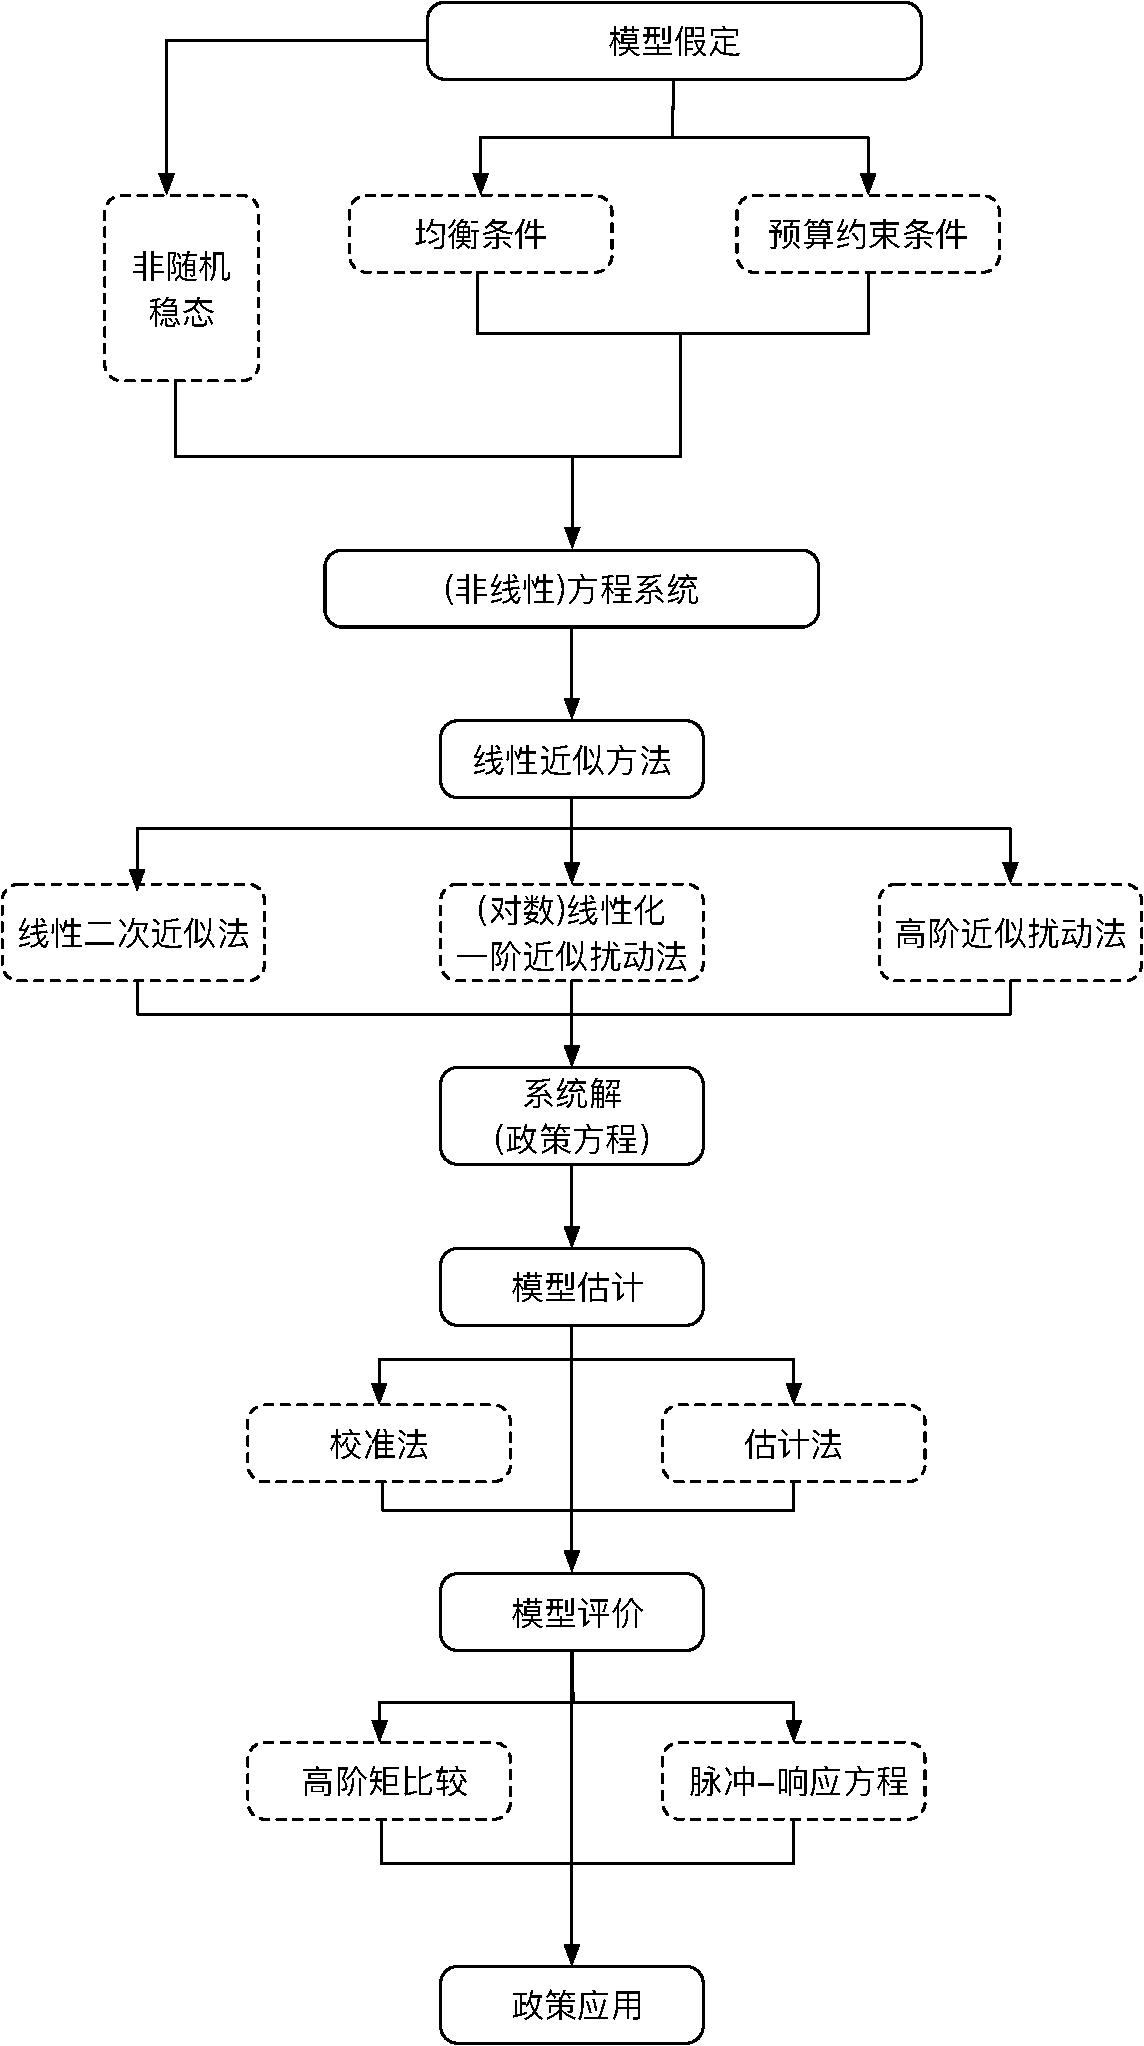
\includegraphics[height=13cm]{./Figures/20170701-DSGE-workflow}
  \label{fig:DSGE-work-flow}
%
%  \small{Source: PBOC.}
\end{figure}

\begin{enumerate}
  \item 构建经济模型(假设条件)。
  \item 求解一阶均衡条件。一阶均衡条件与预算约束条件等一道构成非线性随机差分方程系统。
  \item 由于该系统常常难以求得解析解,需要围绕这一个给定的点做数值近似。这一给定点,常常设定为模型的非随机稳定状态。
  \item 非随机稳定状态可由如下方法之一求得:
  \begin{enumerate}
    \item (对数)线性化近似,围绕稳态,得到一个状态——空间形式表述的线性差分系统,进而借助一些常见算法求得系统的近似数值解;
    \item 围绕非随机稳定状态,做二阶或更高阶的近似。
  \end{enumerate}
  \item 参数校准和/或估计。
  \item 针对外生随机冲击,计算方差、做方差分解,求得有关变量的脉冲——响应方程。
  \item 比较模型生成数据和史记观测到的数据以评价模型的解释力。
  \item 政策参考。
\end{enumerate}
下一节首先讨论模型设定。

\section{模型设定}
模型的前提假定应设定为与所研究的问题密切相关,并且必须指明模型中所讨论的问题是从定性还是定量的角度展开的。围绕所研究的问题,模型应该提供有所助益的回答,如:哪些冲击对经济体产生何种影响,它们的传导机制是怎样的,如何制定相关政策以应对这些冲击?

在一般均衡模型中,经济体中的每一个部门都是单独设定的,典型的部门如私人部门和公共部门:
\begin{enumerate}
  \item 私人部门包括如消费(家庭)部门和企业部门等。通常来说,消费者被简化为一个典型家庭,基于自身偏好,做关于消费和休闲的一生最优决策\citep{Christiano:2010wla}。企业在一定的生产条件限制下追求利润最大化。在为私人部门建模时,必须假定预期的形式,如理性预期或者经验法则等。
  \item 公共部门包括如财政政策和货币政策等。通常来说,政府是财政政策的制定者,大多数情况下财政政策的效果受到李嘉图等价(Ricardian equilvalence)的影响。中央银行设定货币政策。在为公共部门建模时,必须假定政策的执行方式,比如公共部门的政策制定是否依据某准则,是否受某种预算约束条件的限制,行为是否遵循某种利润最大化原则等。
  \item 在经济模型中,个体行动也要受到市场机制和制度性要素的考量,因此也徐作出设定,比如哪些市场是充分/非充分竞争的,决策者的政策制定是否需要遵循一些经验法则等。
  \item 外生随机冲击的识别和建模。
\end{enumerate}
上述模型设定都必须转换成适当的数学表达式,一方面使其能被纳入到模型分析框架中去,另一方面更重要的是,数学表达式的设定需要使模型有解。如,关于偏好和冲击的凹或凸的方程式,非庞兹骗局的约束条件等。

在模型设定后,下一步工作是要针对经济体中的家庭、企业、公共部门等,分别求得一阶最优条件和预算约束条件方程。这些方程常常包括当期和/或前向(后向)元素,又称非线性理性期望系统。通常来说,我们需要借助一定的数值近似方法,将非线性系统做近似线性化,进而求解,这一求解方法的讨论见下节。

\section{求解方法}
对于动态模型如新古典主义经济增长模型,最常见的解法是动态规划(Dynamic Programming),又称价值方程迭代,简要介绍见第\ref{sec:linear-quardratic-control-intro}章。这种方法的优势在于算法可靠度高,解的收敛特性好。但不足也较明显,如计算速度慢,存在维数灾难(curse of dimensionality, \cite{Bellman:1957tx})等\todo{curse of dimensionality,可由映射法得到一定程度上的缓解,做一个reference。}。

动态规划法的不足导致新算法的出现,典型如扰动法(perturbation methods)、投影法(projection methods)等。这些新方法在保持较好收敛特性的基础上,提供了更快的求解速度。扰动法在宏观经济学研究中的广泛应用,综述可见如\cite{Stokey1989,Ljungqvist:2004vz}。投影法的简要介绍见\cite{Aruoba:2006cz}。

本章内容重在对求解方法做简要介绍。大致说来,求解方法分为两步。第一步,近似线性化,将由均衡条件和约束条件构成的非线性方程系统转化为线性方程系统。不同方法背后核心思路基本一致,即将变量围绕其非随机稳定状态附近做线性近似。第二步常常被视为求解DSGE模型的核心,即根据近似线性系统的实际特征,采用相应的数值算法求解,作为原非线性系统的近似解\footnote{扰动法和投影法,从本质上来说都是局域算法。全局算法如车比雪夫多项式(Chebyshev-polynomial)、有限元(finite-elements)等的综述可见\cite{Judd:1998uy}。}。

\subsection{近似线性展开}
在\cite{King:1988bk, King:1988kf, King:2002ih}的开创性工作之后,(对数)线性近似法逐渐成为主要标准。以将变量沿着其非随机稳态做一节泰勒级数展开为例,假定$y=f(x)$,其中$x,y$分别是动态模型中的前定和非前定变量(predetermined and non-predetermined variables),$f$是个平滑的非线性函数\footnote{这里我们采用\cite{Klein:2000bc}的定义:$x_t$是前定变量,当且仅当它有外生的$1$期前向预测偏误,即$x_{t+1} - E_t X_{t+1} = C \varepsilon_{t+1}$是外生的。

根据这一定义,一个前定变量由它的滞后项和当期外生冲击所共同决定,如外生冲击变量。另一方面,不属于此情况的变量成为非前定变量,常常是前向变量。
}。

定义 $x_t$的确定性(非随机)稳定状态为$\bar{x}$,我们有$\bar{y} = \bar{x}$。

对$f$围绕$\bar{x}$做泰勒级数展开
\begin{equation}
  \label{sec:solution-talor-series-expansion-n}
  y \approx \sum_{n=0}^{\infty} \frac{f^{(n)}(\bar{x})}{n!} \left(x-\bar{x} \right)^{n},
\end{equation}
其中$f^{(n)}$表示$f$对$x$的第$n$次求导。

\subsubsection{(1阶)线性化近似}
根据\eqref{sec:solution-talor-series-expansion-n},1阶泰勒级数展开
\begin{equation}
  \label{sec:solution-talor-series-expansion-2-lin}
\begin{split}
    &y \approx f(\bar{x}) + f_x (\bar{x}) (x-\bar{x}), \\
    & \Rightarrow (y-\bar{y}) \approx f_x(\bar{x}) (x - \bar{x}), \\
    & \Rightarrow \frac{y-\bar{y}}{\bar{y}} \approx \frac{f_x (\bar{x}) \bar{x}}{\bar{y}} \frac{x - \bar{x}}{\bar{x}}, \\
    & \Rightarrow \tilde{y} \approx \underbrace{\frac{f_x (\bar{x}) \bar{x}}{\bar{y}}}_{\text{常系数}} \tilde{x},
\end{split}
\end{equation}
根据定义,$\tilde{y}_t$和$\tilde{x}_t$分别表示$y_t$和$x_t$相对于其确定性稳态$\bar{y}$和$\bar{x}$的偏离百分比。

\subsubsection{(1阶)对数线性化近似}
对模型做变型,$y=\exp(\ln y) = f(\exp (\ln x))$。

两侧取对数,$\ln y = \ln f(\exp (\ln x))$。

围绕$\ln \bar{x}$作1阶泰勒级数展开
\begin{equation}
  \begin{split}
    &\ln y \approx \ln f(\exp (\ln \bar{x})) + f_x (\bar{x}) \frac{d \exp(\ln x)}{d \bar{x}}  \left( \ln x - \ln \bar{x} \right), \\
    & \Rightarrow \ln y \approx \ln \bar{y} + f(\exp ( \ln \bar{x})) \left( \ln x - \ln \bar{x} \right), \\
    & \Rightarrow \ln \left(\frac{y}{\bar{y}}\right) \approx \underbrace{\frac{f_x (\bar{x}) \bar{x}}{\bar{y}}}_{\text{常系数}} \ln \left( \frac{x}{\bar{x}} \right),
  \end{split}
  \end{equation}
  其中$\ln \left(\frac{y}{\bar{y}}\right)$和$\ln \left( \frac{x}{\bar{x}} \right)$分别表示对数形式的偏离百分比。

一阶泰勒级数展开后的线性化近似和对数线性化近似,本质上相似。为了说明这一点,见下式
\begin{equation*}
  \tilde{x}_t = \frac{x_t - \bar{x}}{\bar{x}} = \frac{x_t}{\bar{x}} - 1 \approx \ln \left(\frac{x_t}{\bar{x}}\right) = \ln x_t - \ln \bar{x}.
\end{equation*}

此外\cite{Uhlig:1999vx}提出另一种类似对数线性化的方法,从而在特定情况下无需求导:对于常数$a$和接近$0$的$\tilde{x}_t$和$\tilde{y}_t$,
\begin{equation*}
  \begin{split}
    &\exp (x + ay) \approx 1 + x + ay, \\
    &\Rightarrow x y \approx 0, \\
    & \Rightarrow E_t \left( a \exp (x_{t+1}) \right) \approx E_t \left( a x_{t+1} \right).
  \end{split}
\end{equation*}

对数线性化方法的本质在于将变量$x_t$用$x \exp (\tilde{x}_t$来代替,此时$\tilde{x}_t = \ln (x_t/\bar{x})$表示它相对于稳态的对数偏差。利用此方法,可以将非线性方程近似为围绕稳态的线性方程。

\subsubsection{2阶近似}
根据\eqref{sec:solution-talor-series-expansion-n},以2阶展开为例
\begin{equation}
  \label{sec:solution-talor-series-expansion-2}
  y \approx \underbrace{f(\bar{x})}_{\text{0阶展开}} + \underbrace{f_{x}(\bar{x}) (x-\bar{x})}_{\text{1阶展开}} + \underbrace{\frac{1}{2} f_{xx}(\bar{x}) \left(x-\bar{x}\right)^2}_{\text{2阶展开}} + \underbrace{O^3}_{\text{误差项}},
\end{equation}
其中线性近似的误差项$O^3$是由忽略了3阶及以上阶数近似所造成的。

\eqref{sec:solution-talor-series-expansion-2}为代表的线性近似法具有如下特征:
\begin{enumerate}
  \item 在一阶泰勒级数展开中,$y$的条件期望值等于稳态下的$\bar{y}$,这意味着不确定性(以方差的二阶或更高阶矩等形式表现)在线性近似过程中不起作用。
  \item 在高阶泰勒级数展开中,$y$的条件期望值与方程$f$的曲率和变量$x$的方差有关。
  \item 如果研究的目的是求得冲击响应方程以及变量的二阶距,那么我们只分析模型的一阶属性即可,只需要对非线性系统做一阶泰勒级数展开。如,$var(y)$可以通过\eqref{sec:solution-talor-series-expansion-2}算出:$var(y) = E(y = Ey)^2 = f_x^2 var(x)$。
\end{enumerate}

在什么情况下做一阶展开,什么情况下需要做更高阶展开?
\begin{enumerate}
  \item 在很多情况下,对非线性系统做一阶线性近似即可。尽管有研究发现更高阶的近似会提供更精确的近似解,但精读提升的幅度有限。
  \item 然而的确存在一些情况,仅仅用一阶近似处理DSGE模型是不够的,尤其是当研究目标涉及到分析一些政策的福利效果时——这些福利政策往往不会对模型产生一阶影响。
\end{enumerate}
我们将在随后章节中进一步展开探讨这个问题\todo{加入一个reference。}。

对非线性方程系统做线性近似,生成以状态——空间形式表现的变型系统。这样,一方面可以更方便的展开后续经验研究,如模型估计,卡曼滤波,经济系统预测等。更为重要的是另一方面,搭配一些数值求解方法,可以求得系统的近似解。随后我们讨论如何在理性预期的情境下,运用数值算法求解变型系统。

\section{求解线性随机差分方程系统}
如前文所述,由各部门均衡条件和预算约束条件所组成的非线性系统,经由一定的(对数)线性化处理后变型为新的系统,又称线性随机方程差分系统,

新系统有一组含有理性期望条件的线性随机差分方程构成,可表述为如下状态——空间形式,
\begin{equation}
  \label{eq:solution-lin-stho-diff-eq}
  A_0 E_t Y_{t+1} = A_1 Y_t + B_0 \varepsilon_1,
\end{equation}
其中$A_0, A_1, B_0$是线性化系统的系数矩阵,$Y_t, \varepsilon_t$分别是内生变量和外生变量构成的向量。

在构建DSGE模型时,外生变量$\varepsilon_t$常取如下两个假定之一。假定$\varepsilon_t$是iid冲击向量,$E(\varepsilon_t) = 0, E(\varepsilon_t \varepsilon_t^{\top}) = \Sigma, E(\varepsilon_t \varepsilon_s^{\top}) = \Sigma \forall s \neq t$,或者假定$\varepsilon_t$是与iid外生冲击有关的$AR(1)$过程。

这样一个线性化方程构成的动态系统,描述了模型中变量的运动路径。通常来说系统中含有前向及后向要素\todo{Karl Whelan对 forward-looking和backward-looking的描述}。随着模型参数设定的不同,系统解存在三种情况:
\begin{itemize}
  \item 无解。系统没有稳定的理性预期解。
  \item 不确定(indeterminacy)。系统存在不止一个解的多重均衡。
  \item 确定的。有且只有一个解,又称稳定解。
\end{itemize}
如果前两种情况出现,意味着模型参数设定不当,需要重新调整,以使得系统存在稳定解。

已经有大量文献探讨理性期望系统\eqref{eq:solution-lin-stho-diff-eq}的求解方法。系统的解构成一个回应机制(feedback rule),将当期内生变量与模型内的状态变量联系起来。这方面的重要工作框架由\cite{Blanchard:1980gi}所奠定,随后经由许多人的努力,得到进一步深化和扩展,见第\ref{sec:rational-exp-chap}章。

如果DSGE模型致力于考察政策的福利效果,如期望效用等,则仅仅用一阶近似线性转换可能不够精确。此时需要对效用函数等其他函数做二阶近似,以确保二次项所含有的重要经济学信息不被忽略掉\citep{Kim:2003hf,SchmittGroh:2004da},见第\ref{sec:ptb}章。

%!TEX root = ../DSGEnotes.tex
\chapter{动态规划}
\label{sec:dp}

简要介绍动态规划(dynamic programming)\index{dynamic programming \dotfill 动态规划}。更详细的介绍,见\cite{Adda:2003tt}。Python中的程序实现见\cite{Stachurski:2008wc}。

\section{包络定理}
\label{sec:dp-envelope-theorem}
包络定理(Envelope Theorem)\index{Envelope Theorem \dotfill 包络定理}研究当模型中的参数发生变化时,模型中某一变量的最大值(或最小值)如何随着发生变化。
\begin{theorem}[包络定理]
  \label{theorem:envelope-theorem}
  假定我们有
  \begin{equation}
  \label{eq:dp-envelope-value-def}
  v(a)= \max_{\{x\}} f(x,a),
\end{equation}

那么下式成立
\begin{equation}
  \label{eq:dp-envelope-partial}
  \frac{d v(a)}{d a} = \frac{\partial f(x,a)}{\partial a} \Big|_{x = x^{*}(a)},
\end{equation}
其中
\begin{equation}
  \label{eq:dp-envelope-def-xstar}
  x^{*}(a) = \mathop{\arg \max}_{\{x\}} f(x,a).
\end{equation}
\end{theorem}

\begin{proof}
设
\begin{equation*}
  v(a) \equiv f \left[ x^{*}(a), a \right],
\end{equation*}
两侧同时对$a$求(偏)导
\begin{equation}
  \label{eq:dp-envelope-partial-both}
  \frac{d v(a)}{d a}
  = \frac{\partial f \left[ x^{*}(a), a \right] }
  {\partial x}
  \frac{\partial x^{*}(a)}
  {\partial a}
  + \frac{\partial f \left[ x^{*}(a), a \right] }
  {\partial a}.
\end{equation}

上式中$x^{a}$是$f(x,a)$取极大值时的系数,满足
\begin{equation*}
  \frac{\partial f \left[ x^{a}, a \right]}{\partial x}=0,
\end{equation*}
代回\eqref{eq:dp-envelope-partial-both}有

\begin{equation}
  \label{eq:dp-envelope-partial-both-2}
  \frac{d v(a)}{d a}
  = \frac{\partial f \left[ x^{*}(a), a \right] }
  {\partial a},
\end{equation}
等价于\eqref{eq:dp-envelope-partial}.
\end{proof}

或者也可以从有约束条件的优化问题中推得包络定理
\begin{theorem}[包络定理(有约束条件的优化问题)]
  \label{theorem:envelope-theorem-constraint}
    设
    \begin{equation*}
      \begin{split}
        m(a) & = \max_{\{x\}} f(x,a), \\
        & s.t. \begin{cases}
        g(x,a)=0, \\
        x \ge 0.
        \end{cases}
      \end{split}
    \end{equation*}

    使$\mathcal{L} \left( x,a,\lambda \right)$为相应的拉格朗日方程,其中$x^{*}(a), \lambda^{*}(a)$为库恩塔克条件(Kuhn-Tucker condition)的最优解。则我们有
    \begin{equation}
      \label{eq:envelope-theorem-constraint}
      \frac{d m(a)}{d a} = \frac{\mathcal{L}(a)}{\partial a} \Big|_{x^{*}(a), \lambda^{*}(a)}.
    \end{equation}
\end{theorem}

\section{例:吃蛋糕(直接求解法)}
\label{sec:dp-cake}
小明有一块蛋糕,大小是$W_{1}$,可以在$t=1,2,\ldots,T$期内吃完。问小明怎么吃可以实现效用最大化?

小明的最优决策可以表现为贴现效用的求和加总
\begin{equation*}
  \sum_{t=1}^{T} \beta^{t-1} u(c_t),
\end{equation*}
其中$c_{t}$表示$t$期消费即吃掉蛋糕的大小。$u(c_{t})$表示$t$期效用,设方程满足可导、严格单调、严格凹(concave),即稻田条件(Inada condition)\index{Inada condition \dotfill 稻田条件}\citep{Inada1963}
\begin{equation*}
  \lim_{c \rightarrow 0} u'(c) \rightarrow \infty, \quad \lim_{c \rightarrow \infty} u'(c) \rightarrow 0.
\end{equation*}
引入稻田条件的作用是确保小明每个时段$t$都至少会吃一小口蛋糕,即从数学角度上来讲,不存在角点解(corner solution)。蛋糕的大小随时间发生变化,满足
\begin{equation}
  \label{eq:dp-cake-size-motion}
  W_{t+1} = W_{t} - c_{t}, \quad t = 1,2,\ldots, T.
\end{equation}

若是按照直接求解法的思路,小明吃蛋糕问题可以表示为
\begin{equation*}
  \max_{
  \left\{c_{t}\right\}_{t=1}^{T}, \,
  \left\{W_{t}\right\}_{t=1}^{T+1}
  }
  \sum_{t=1}^{T} \beta^{t-1} u \left( c_{t} \right),
\end{equation*}
给定约束条件
\begin{equation*}
%  \label{eq:dp-cake-direct-constraint}
  \begin{split}
    \sum_{t=1}^{T} c_{t} + \sum_{t=1}^{T} W_{t+1} = \sum_{t=1}^{T} W_{t}, \\
    \Rightarrow \sum_{t=1}^{T} c_{t} + W_{T+1} = W_{t},
  \end{split}
\end{equation*}
即小明吃掉的所有蛋糕,和最终剩余的蛋糕数量$W_{T+1}$之和,等于蛋糕的初始大小$W_{1}$。

鉴于此,可以将问题改写为
\begin{equation}
  \label{eq:dp-cake-direct-problem}
  \max_{
  \left\{c_{t}\right\}_{t=1}^{T}, \,
  \left\{W_{t}\right\}_{t=2}^{T+1}
  }
  \sum_{t=1}^{T} \beta^{t-1} u \left( c_{t} \right),
\end{equation}
约束条件为
\begin{equation}
  \label{eq:dp-cake-direct-constraint}
  \begin{cases}
    \sum_{t=1}^{T} c_{t} + W_{T+1} = W_{1}, \\
    c_{t} \ge 0 \quad \forall \, t = 1,\ldots,T,\\
    W_{T+1} \ge 0.
  \end{cases}
\end{equation}
在随后的分析中我们不再讨论$c_{t} \ge 0$的约束条件,因为假定稻田条件$\lim_{c \rightarrow 0} \, u'(c) \rightarrow \infty$成立,就已经满足该项。

构建拉格朗日方程方程
\begin{equation*}
  \mathcal{L} = \sum_{t=1}^{T} \beta^{t-1} u \left( c_{t} \right) + \lambda_{t}
  \left[
    W_{1} - \sum_{t=1}^{T} c_{t} - W_{T+1}
  \right]
  + \phi_{t} W_{T+1}.
\end{equation*}

两个一阶条件FOCs给出最大化问题的解
\begin{itemize}
  \item
  \begin{equation}
  \label{eq:dp-cake-foc-c}
  \frac{\partial \mathcal{L}}{\partial c_{t}} = 0 \Rightarrow \beta^{t-1} u' \left( c_{t} \right) = \lambda_{t}, \quad t = 1,\ldots, T,
\end{equation}
其中拉格朗日乘子$\lambda_{t}$对应预算约束条件,\eqref{eq:dp-cake-direct-constraint}第一行,即
\begin{equation*}
  \lambda_{t} = \beta^{t} u' \left( c_{t+1} \right).
\end{equation*}
将两期最优消费决策联系起来,可得
\begin{equation}
  \label{eq:dp-cake-euler}
  u'(c_{t}) = \beta u'(c_{t+1}),
\end{equation}
这称为跨(1)期消费的欧拉等式(Euler equation)。

\item
\begin{equation}
  \label{eq:dp-cake-foc-w}
  \frac{\partial \mathcal{L}}{\partial W_{T+1}} =0 \Rightarrow \lambda_{t} = \phi_{t},
\end{equation}
其中拉格朗日乘子$\phi_{t}$对应横截条件,\eqref{eq:dp-cake-direct-constraint}第三行。已知根据稻田条件的,$\lambda_{t} > 0$严格成立,则$\phi_{t} > 0 \, \forall t$。这意味着若要满足库恩塔克(Kuhn-Tucker condition)
\begin{equation}
  \label{eq:dp-cake-kuhn-tucker}
  \phi_{t} W_{T+1} =0,
\end{equation}
只能使得$W_{T+1} \equiv 0$。
\end{itemize}

进一步解读欧拉等式\eqref{eq:dp-cake-euler}。在均衡状态下,当期$t$减少1单位消费的边际效用下降,应当等于$t$期额外1单位储蓄的增加,在$t+1$期带来边际效用提升的贴现值。将跨1期扩展到跨多期的情况,任意两期$t,t'$之间$t,t'=1,\ldots,T, \, t' > t$的跨期消费转移都不会导致总福利水平的变化。这样一来,(已经处于最优行为决策下的)小明,全部福利水平最大便只取决于初始蛋糕的大小$W_{1}$,对应福利$V_{T} \left( W_{1} \right)$,又称价值方程(value function)\index{value function \dotfill 价值方程}:
\begin{equation}
  \label{eq:dp-cake-value-function}
  V_{T} \left( W_{1} \right)
  = \max_{ \left\{ c_{t} \right\}_{t=1}^{T}}
  \sum_{t=1}^{T} \beta^{t-1} u \left( c_{t} \right)
  + \lambda_{t} \left[ W_{1} - \sum_{t=1}^{T} c_{t} - W_{T+1} \right] + \phi_{t} W_{T+1},
\end{equation}

那么为了回答初始蛋糕大小$W_{t}$对小明总福利水平$V_{T} \left( W_{1} \right)$的影响,可以求导数
\begin{equation*}
  \frac{d V_{T} \left(W_{1} \right)}{d W_{1}}
  = V_{T}^{'} \left( W_{1} \right) = \lambda_{t}.
\end{equation*}

\section{吃蛋糕(动态规划)}
\label{sec:dp-cake-dy}

\subsection{有限时间段的动态规划问题}
\label{sec:dp-cake-finite}
我们先从容易理解的$T < \infty$入手,熟悉动态规划问题的基本原理。然后将问题扩展到$T \rightarrow \infty$的情况,见第\ref{sec:dp-cake-finite}节。

从$t=1$期来看,给定$W_{1}$,吃蛋糕问题可以改写为如下形式
\begin{equation}
  \label{eq:dp-cake-fin-prob}
  V_{T} \left( W_{1} \right) = \max_{\left\{ c_{t}\right\}_{t=1}^{T}} u \left( c_{1} \right)+ \beta V_{T-1} \left(W_{2} \right), \quad \, W_{2} = W_{1} - C_{1},
\end{equation}
$t=1$期小明的决策是,消费多少蛋糕$c_{1}$,这会传导到$t=2$期影响到$W_{2}$;以此类推。那么,$c_{t}$最优消费决策应当使$t$期效用的变化,与$t+1$期效用变化的贴现相等,这称为贝尔曼等式(Bellman equation)\index{Bellman equation \dotfill 贝尔曼等式}。

另一方面,对贝尔曼等式\eqref{eq:dp-cake-fin-prob}求FOC,可得欧拉等式
\begin{equation}
  \label{eq:dp-cake-fin-foc}
  u'\left( c_{1} \right)   = \beta V_{T-1}^{'} \left(W_{2} \right).
\end{equation}

现在设效用函数的显形式为$u(c) = \ln c$,那么通过逆推法,可以进一步计算价值方程。

$T=1$时,小明的最优决策是当期吃掉全部蛋糕,$c_{1}=W_{1}$,因此我们有
\begin{equation}
  \label{eq:dp-cake-fin-t-1}
  V_{1} \left( W_{1} \right) = \ln W_{1}.
\end{equation}

$T=2$时,小明的最优决策根据\eqref{eq:dp-cake-fin-prob}表示为
\begin{equation}
  \label{eq:dp-cake-fin-t-2}
  V_{2} \left( W_{1} \right) = \max_{W_{2}} \underbrace{
  \ln \left( W_{1} - W_{2} \right)
  }_{u(c_{1})} + \beta \underbrace{
  \ln W_{2}
  }_{u(c_{2})},
\end{equation}

约束条件
\begin{equation}
  \label{eq:dp-cake-fin-t-2-euler}
  c_{1}+ W_{2} = c_{1} + c_{2} = W_{1},
\end{equation}

欧拉等式
\begin{equation*}
  u' \left( c_{1} \right) = \beta V_{2}^{'} \left( W_{1} \right),
\end{equation*}

FOC
\begin{equation}
  \label{eq:dp-cake-fin-t-2-foc}
  \frac{1}{c_{1}} = \beta \frac{1}{c_{2}},
\end{equation}

联立\eqref{eq:dp-cake-fin-t-2-euler}和\eqref{eq:dp-cake-fin-t-2-foc}可得最优消费决策$\left\{ c_{t} \right\}_{t=1}^{2}$
\begin{equation}
  c_{1} = \frac{1}{1+\beta} W_{1}, \quad c_{2} = \frac{\beta}{1+\beta} W_{1},
\end{equation}

价值方程因此为
\begin{equation}
  \label{eq:dp-cake-fin-t-2-value-function}
  V_{2} \left( W_{1} \right) =
  \ln
  \left(
  \frac{1}{1+\beta} W_{1}
  \right)
  + \beta \ln
  \left(
  \frac{\beta}{1+\beta} W_{1}
  \right),
\end{equation}
有时我们将其进一步简化为
\begin{equation*}
  \begin{split}
  & V_{2} \left( W_{1} \right)
  = A_{2} + B_{2} \ln W_{2}, \\
  & A_{2} = \ln \left( \frac{1}{1 + \beta} \right)+ \beta \ln \left( \frac{\beta}{1+\beta} \right), \\
  & B_{2} = 1+\beta.
  \end{split}
\end{equation*}

$T=3$时,小明的最优决策分三部分,依次为
\begin{enumerate}
  \item
  \begin{equation}
    \label{eq:dp-cake-fin-t-3-A}
    V_{3} \left( W_{1} \right)
    = \max_{W_{2}} \underbrace{
    \ln \left( W_{1} - W_{2} \right)
    }_{u \left( c_{1} \right)}
    + \beta V_{2} \left( W_{2} \right),
  \end{equation}

  FOC
  \begin{equation}
    \label{eq:dp-cake-fin-t-3-A-foc}
    V_{3}^{'} \left( W_{1} \right) = 0 \Rightarrow \frac{1}{c_{1}} = \beta V_{2}^{'} \left( W_{2} \right).
  \end{equation}

  \item
  \begin{equation}
    \label{eq:dp-cake-fin-t-3-B}
    V_{2} \left( W_{2} \right)
    = \max_{W_{3}} \underbrace{
    \ln \left( W_{2} - W_{3} \right)
    }_{u \left( c_{2} \right)}
    + \beta V_{1} \left( W_{3} \right),
  \end{equation}

  FOC
  \begin{equation}
    \label{eq:dp-cake-fin-t-3-B-foc}
    V_{2}^{'} \left( W_{2} \right) = 0 \Rightarrow \frac{1}{c_{2}} = \beta V_{1}^{'} \left( W_{3} \right).
  \end{equation}

  包络条件
  \begin{equation}
    \label{eq:dp-cake-fin-t-3-B-envelope}
    \frac{1}{c_{2}} = V_{2}^{'} \left( W_{2} \right).
  \end{equation}

  \item
  \begin{equation}
    \label{eq:dp-cake-fin-t-3-C}
    V_{1} \left( W_{3} \right)
    = \ln W_{3},
  \end{equation}
  因为$W_{4}=0$。

  FOC
  \begin{equation}
    \label{eq:dp-cake-fin-t-3-C-foc}
    V_{1}^{'} \left( W_{3} \right) = 0 \Rightarrow \frac{1}{c_{3}} = V_{1}^{'} \left( W_{3} \right).
  \end{equation}
\end{enumerate}

在此基础上我们有,我们可以用逆推的方法求得最优消费决策$\left\{ c_{t} \right\}_{t=1}^{3}$
\begin{enumerate}
  \item 联立\eqref{eq:dp-cake-fin-t-3-B-foc}和\eqref{eq:dp-cake-fin-t-3-C-foc}可得
  \begin{equation*}
    \frac{1}{c_{2}} = \beta \frac{1}{c_{3}},
  \end{equation*}

  \item 联立\eqref{eq:dp-cake-fin-t-3-A-foc}和\eqref{eq:dp-cake-fin-t-3-B-envelope}可得
  \begin{equation*}
    \frac{1}{c_{1}} = \beta \frac{1}{c_{2}},
  \end{equation*}

  \item 资源约束条件
  \begin{equation*}
    c_{1} + c_{2} + c_{3} = W_{1}.
  \end{equation*}
\end{enumerate}

因此我们有
\begin{equation*}
  \begin{split}
    c_{1} = \frac{1}{1+\beta+\beta^{2}} W_{1}, \\
    c_{2} = \frac{\beta}{1+\beta+\beta^{2}} W_{1}, \\
    c_{3} = \frac{\beta^{2}}{1+\beta+\beta^{2}} W_{1},
  \end{split}
\end{equation*}
对应的价值方程为
\begin{equation}
  \label{eq:dp-cake-fin-t-3-value-function}
  V_{3} \left( W_{1} \right)
  = \ln c_{1} + \beta \left( \ln c_{2} + \beta \ln c_{3} \right).
\end{equation}


\subsection{无限时间段的动态规划问题}
\label{sec:dp-cake-infinite}
随着$T \rightarrow \infty$,无法再使用上一节介绍过的逆推法,情况变得较为复杂。无限时间段的吃蛋糕问题,小明追求效用最大化
\begin{equation*}
  \begin{split}
    & \max_{\left\{ c_{t} \right\}_{t=1}^{\infty}, \, \left\{ W_{t} \right\}_{t=2}^{\infty}}
    \sum_{t=1}^{\infty} \beta^{t-1} u \left( c_{t} \right), \\
    & \text{s.t.} \, W_{t+1} = W_{t} - c_{t}, \quad t = 1,2,\ldots
  \end{split}
\end{equation*}

我们将这个问题改写为动态规划的形式
\begin{equation*}
%  \label{eq:dp-cake-infin-problem}
  V \left( W \right) = \max_{c \in \left[ 0, W \right]} u(c) + \beta V \left( W - c \right),
\end{equation*}
其中$V \left( W \right)$为当期小明采取最优行为决策所可能得到的最大效用;$V \left( W - c \right)$为下期小明采取最优行为决策所可能得到的最大效用:显然,$c$是控制变量,$W$是状态变量。设$W' \coloneqq W-c$,那么动态规划问题改写为如下贝尔曼等式形式的泛函方程
\begin{equation}
  \label{eq:dp-cake-infin-problem}
  V \left( W \right) = \max_{W' \in \left[ 0, W \right]} u \left( W - W' \right) + \beta V \left( W' \right).
\end{equation}


求解无限时段的动态规划问题\eqref{eq:dp-cake-infin-problem}可分三部,核心思路是找到一个$V \left( W \right)$使得对于所有$W$的值,泛函式均成立。出于简化模型的考虑,我们取消时间下角标——因为在无限时段下,这成为一个静态(stationary)或者无关时间(time-invariant)的问题。三部如下
\begin{enumerate}
  \item \eqref{eq:dp-cake-infin-problem}的FOC
  \begin{equation}
    \label{eq:dp-cake-infin-foc}
    V' \left(W \right) = 0 \Rightarrow u'(c) = \beta V' \left( W' \right).
  \end{equation}

  难点:在不清楚原方程形式$V(W)$的情况下,如何计算$V'(W')$。

  \item 包络条件
  \begin{equation}
    \label{eq:dp-cake-infin-envelope}
    V'\left( W \right) = u'(c) \Leftrightarrow V'(W') = u'(c').
  \end{equation}
  包络条件的前提是假定行为人处于最优决策条件下。

  \item 联立FOC\eqref{eq:dp-cake-infin-foc}和包络条件\eqref{eq:dp-cake-infin-envelope}
  \begin{equation}
    u'(c) = \beta u'(c'),
  \end{equation}
  即欧拉等式。由此我们可以定义一组策略方程
  \begin{equation}
    \label{eq:dp-cake-infin-envelope-policies}
    \begin{split}
      c & = \phi \left(W \right), \\
      W' & = e \left(W \right) = W - \phi \left( W \right),
    \end{split}
  \end{equation}
使满足欧拉等式
\begin{equation}
  \label{eq:dp-cake-infin-envelope-euler}
  u' \left( \phi (W) \right) = \beta u'
  \left(
  W - \phi (W)
  \right).
\end{equation}
\end{enumerate}

现在以$u(c) = \ln c$为例做进一步求解\footnote{通常来说,我们无法求得价值方程的显性形式,但$u(c) = \ln c$可能是少数的例外之一。}。首先,我们猜测$V(W)$可能是以下线性形式
\begin{equation}
  \label{eq:dp-cake-infin-envelope-value-guess}
  V(W) = A + B \ln W,
\end{equation}
线性形的猜测是为了让计算过程简化,更多非线性形的讨论可见\cite{Hansen:2004va}。代回\eqref{eq:dp-cake-infin-problem}可得
\begin{equation}
  \label{eq:dp-cake-infin-envelope-value}
  A + B \ln W = \max_{W' \in \left[ 0, W \right]}
  u \left( W - W' \right) + \beta V \left( A + B \ln W' \right).
\end{equation}

类似地,取FOC作为最优条件
\begin{equation*}
  \begin{split}
    & \frac{1}{W - W'} = \beta B \frac{1}{W'}, \\
    & \hookrightarrow W' = \frac{\beta B}{1 + \beta B} W,
  \end{split}
\end{equation*}
代回\eqref{eq:dp-cake-infin-envelope-value}可得
\begin{equation}
  \label{eq:dp-cake-infin-envelope-ABvalue}
  \begin{split}
  A + B \ln W & =
  \ln \left( \frac{W}{1 + \beta B} \right)
  + \beta \left[
  A + B \ln \left( \frac{\beta B}{1 + \beta B} W \right)
  \right] \\
  & = \ln W - \ln \left(1 + \beta B \right) + \beta A + \beta B \ln \left( \frac{\beta B}{1 + \beta B} \right) + \beta B \ln W \\
  & = \underbrace{
  - \left[ \ln \left( \beta B \right) + 1 \right] \ln \left( 1 + \beta B \right)
  + \beta \left[
  A + B \ln \left( \beta B \right)
  \right]
  }_{A}
  +
  \underbrace{
  \left( 1 + \beta B \right)
  }_{B}
  \ln W,
  \end{split}
\end{equation}

LHS和RHS相对应,可得系数A B的值
\begin{equation*}
  \begin{split}
    A & = \frac{1}{\left( 1 - \beta \right)^{2}}
    \left\{
    \beta \ln \left( \frac{\beta B}{1 - \beta} \right)
    - \left( 1 - \beta \right)
    \ln \left( \frac{1}{1- \beta } \right)
    \left[ 1 + \ln \left( \frac{\beta}{1 - \beta} \right) \right]
    \right\}, \\
    B & = \frac{1}{1 - \beta},
  \end{split}
\end{equation*}

这样我们最终得到了策略方程\eqref{eq:dp-cake-infin-envelope-policies}的计算式
\begin{equation}
  \label{eq:dp-cake-infin-envelope-policies-2}
  \begin{split}
    c & = \phi \left(W \right) = \left( 1 - \beta \right) W , \\
    W' & = e \left(W \right) = \beta W,
  \end{split}
\end{equation}

\section{随机问题}
\label{sec:dp-sthochastic}
现在将不确定性引入动态规划问题的分析中去,如外生偏好冲击,效用函数变为$\varepsilon_{t} u(c_{t})$,其中$\varepsilon$是一个随机变量。在$t$期做最优消费决策的行为人知道当期的$\varepsilon_{t}$,但不掌握对未来期$\varepsilon$的全部信息。一个最简单的设定是$\varepsilon \in \left\{ \varepsilon_{l}, \varepsilon_{h} \right\}$,两种冲击状态满足$\varepsilon_{h} > \varepsilon_{l} > 0$。

偏好冲击表现为一阶马尔科夫过程,即当期冲击状态遇上一期的冲击水平有关。我们常用\cite{Tauchen:1986gi}等方法将AR(1)过程做离散化处理,见第\ref{sec:pj-local-discretization}节。用$p_{ij}$表示当期冲击状态$\varepsilon_{i}$在下一期变为$\varepsilon_{j}$的概率,据此可以构建完整的转移矩阵P,其中的元素例如$p_{lh} \equiv Pr \left( \varepsilon' = \varepsilon_{h} \big| \varepsilon = \varepsilon_{l} \right)$:
\begin{table}[htbp]
\label{table:dp-cake-infin-transmission-matrix}
\caption{偏好冲击的转移矩阵}
\begin{center}
\begin{tabular}{llll}

 &  & \multicolumn{ 2}{c}{$t+1$} \\
 &  & $\varepsilon_{h}$ & $\varepsilon_{l}$ \\ \cline{ 3- 4}
\multicolumn{1}{c}{$t$} & $\varepsilon_{h}$ & $p_{hh}$ & $p_{hl}$ \\ \cline{ 3- 4}
\multicolumn{ 1}{l}{} & $\varepsilon_{l}$ & $p_{lh}$ & $p_{ll}$ \\ \cline{ 3- 4}%\hline
\end{tabular}
\end{center}
\end{table}

这样,随机吃蛋糕问题就变为
\begin{equation*}
  \begin{split}
    V \left( W, \varepsilon \right)
    = \max_{W'} \varepsilon u \left( W - W' \right)
    + \beta E_{\varepsilon' | \varepsilon} V \left( W', \varepsilon' \right), \quad \varepsilon \in  \left\{ \varepsilon_{l}, \varepsilon_{h} \right\},
  \end{split}
\end{equation*}
对应转移矩阵$P$。

FOC描述最优状态
\begin{equation}
  \label{eq:dp-cake-sthochastic-foc}
  \varepsilon u' \left( W - W' \right)
  = \beta E_{\varepsilon' | \varepsilon} V \left(
  W', \varepsilon' \right)
\end{equation}

由包络定理可得
\begin{equation*}
  V_{1}\left(W, \varepsilon \right)
  = \varepsilon u' \left( W - W' \right),
\end{equation*}
进而我们有
\begin{equation}
  \label{eq:dp-cake-sthochastic-t1-t2}
  V_{1} \left(W', \varepsilon' \right)
  = E_{\varepsilon' | \varepsilon}
  \varepsilon' u' \left( W' - W'' \right).
\end{equation}

联立包络定理\eqref{eq:dp-cake-sthochastic-t1-t2}和FOC条件\eqref{eq:dp-cake-sthochastic-foc}可得跨(多)期欧拉等式
\begin{equation}
  \label{eq:dp-cake-sthochastic-euler}
  \varepsilon u' \left( W - W' \right)
  = \beta E_{\varepsilon' | \varepsilon} \varepsilon' u' \left( W' - W'' \right).
\end{equation}

如果我们设政策方程满足一定形式(常常设为线性形)
\begin{equation*}
  W' = \varphi \left( W, \varepsilon \right),
\end{equation*}
代回\eqref{eq:dp-cake-sthochastic-euler},欧拉等式变为
\begin{equation}
  \label{eq:dp-cake-sthochastic-euler-approx}
  \varepsilon u' \left( W - \varphi \left( W, \varepsilon \right) \right)
  = \beta E_{\varepsilon' | \varepsilon} \varepsilon' u' \left\{
  \varphi \left( W, \varepsilon \right) -
  \varphi \left(
  \varphi \left( W, \varepsilon \right), \varepsilon'
  \right)
  \right\}.
\end{equation}

\section{包络定理和欧拉等式的关系}
\label{sec:dp-euler-relation}
上文以小明吃蛋糕问题为例,对动态规划做了一般性介绍。下面以常见的NCGT(Neo-Classical Growth Model,如Ramsey Model)为例,介绍家庭部门的多期优化问题,它是动态经济学模型的基础组成部分之一。

$t$期行为人的目标,追求$t, t+1, \ldots, T$的效用最大化
\begin{equation}
  \label{eq:dp-euler-relation-problem}
  \begin{split}
  & \max \sum_{n=0}^{T-t} \beta^{n} u \left(c_{t+n} \right), \\
  & m_{t+1} = \left( m_{t} - c_{t} \right) R + y_{t+1}.
\end{split}
\end{equation}

根据动态规划的思路,将问题改写为贝尔曼等式形式
\begin{equation}
  \label{eq:dp-growth-bellman}
  V_{t} \left( m_{t} \right)
  = \max_{\left\{ c_{t} \right\} }
  u \left( c_{t} \right)
  + \beta V_{t+1} \left[ \left( m_{t} - c_{t}  \right) R + y_{t+1} \right].
\end{equation}

FOC得到最优条件
\begin{equation*}
  0 = u' \left( c_{t} \right) +
  \left( \frac{d m_{t+1}}{d c_{t}} \right)
  \beta V_{t+1}^{'} \left( m_{t+1} \right),
\end{equation*}
其中$\left( \frac{d m_{t+1}}{d c_{t}} \right) = - R$,$R$反映在\eqref{eq:dp-euler-relation-problem}中。因此上式变为
\begin{equation}
  \label{eq:dp-growth-relation}
  u' \left( c_{t} \right) = \beta R  V_{t+1}^{'} \left( m_{t+1} \right).
\end{equation}

根据\eqref{eq:dp-euler-relation-problem},行为人基于已有的信息$m_{t}$做出当期消费决策$c_{t}$,因此可以定义一个方程
\begin{equation}
  \label{eq:dp-growth-approx-consumption}
  c_{t} = c_{t} \left( m_{t} \right),
\end{equation}
用于描述在给定$m_{t}$时,行为人可以达到效用最大化的最有消费决策。\eqref{eq:dp-growth-approx-consumption}代回\eqref{eq:dp-growth-relation},写为
\begin{equation}
  \label{eq:dp-growth-approx-consumption-approx}
  u' \left( c_{t} \left( m_{t} \right) \right)
  - \beta R V_{t+1}^{'} \left(
  \left[ m_{t} - c_{t} \left( m_{t} \right) \right] R + y_{t+1}
  \right)=0.
\end{equation}
上式中的两个方程都是一阶形式;在原方程形式未知的情况下很难直接求解。我们因此采取近似算法。

定义一个新的方程
\begin{equation}
  \label{eq:dp-growth-value-approx}
  \underline{V}_{t} \left( m_{t}, c_{t} \right)
  = u(c_{t}) + \beta \underline{V}_{t+1}
  \left(
  \left(m_{t} - c_{t} \right) R + y_{t+1}
  \right),
\end{equation}
同样地,对上式求偏导我们有
\begin{align}
  \label{eq:dp-growth-value-approx-foc-c}
  \underline{V}_{t}^{c} & \equiv \frac{\partial \underline{V}_{t}}{\partial c_{t}}
  = u'(c_{t}) - \beta R \underline{V}_{t+1}^{c}
  \left(
  \left(m_{t} - c_{t} \right) R + y_{t+1}
  \right), \\
  \label{eq:dp-growth-value-approx-foc-m}
  \underline{V}_{t}^{m} & \equiv \frac{\partial \underline{V}_{t}}{\partial m_{t}}
  = \beta R \underline{V}_{t+1}^{m} \left( m_{t+1} \right).
\end{align}

根据定义式\eqref{eq:dp-growth-value-approx},结合\eqref{eq:dp-growth-bellman}可见
\begin{equation}
  \label{eq:dp-growth-value-equivalence}
  V_{t} \left( m_{t} \right) = \underline{V}_{t} \left( m_{t}, c_{t} \right),
\end{equation}
引入链式法则(Chain rule)\eqref{eq:chain-rule-exa},上式变为
\begin{equation}
  \label{eq:dp-growth-value-equivalence-derivative}
  \begin{split}
  V_{t}^{'} \left( m_{t} \right) & \equiv V_{t}^{m} \left( m_{t} \right) \equiv \frac{d V_{t} \left(m_{t} \right)}{d m_{t}} \\
  & = \underline{V}_{t}^{m} \left( m_{t}, c_{t} \left( m_{t} \right) \right)
  + \frac{\partial c_{t} \left( m_{t} \right)}{\partial m_{t}}
  \underline{V}_{t}^{c} \left(
  m_{t}, c_{t} \left( m_{t} \right)
  \right).
  \end{split}
\end{equation}

理解\eqref{eq:dp-growth-value-equivalence-derivative}的一个关键是:行为人是处于最优决策状态的,这意味着他总是在衡量价值方程,以及价值方程相对于消费的偏导,使其满足最优条件\eqref{eq:dp-growth-approx-consumption-approx}。\footnote{有时这种最优决策也会受到资源约束条件的限制,如流动性约束等,我们在这里暂不讨论这种情况。},这使得\eqref{eq:dp-growth-value-approx-foc-c}中的$\underline{V}_{t}^{c} = 0$,即
\begin{equation}
  \label{eq:dp-growth-value-approx-foc-c-2}
  u'(c_{t}) = \beta R \underline{V}_{t+1}^{c}
  \left(
  \left(m_{t} - c_{t} \right) R + y_{t+1}
  \right),
\end{equation}
代回\eqref{eq:dp-growth-value-equivalence-derivative}变为
\begin{equation}
  \label{eq:dp-growth-value-equivalence-derivative-2}
  V_{t}^{'} \left( m_{t} \right)
  = V_{t}^{m} \left( m_{t}, c_{t} \left(m_{t} \right) \right) = \beta R V_{t+1}^{m} \left( m_{t+1} \right).
\end{equation}

此外\eqref{eq:dp-growth-value-equivalence-derivative-2}的RHS和\eqref{eq:dp-growth-relation}的RHS相等,因此有
\begin{equation}
  \label{eq:dp-growth-derivative-equiv}
  V_{t}^{'} \left( m_{t} \right) = u' \left( c_{t} \right).
\end{equation}

结合\eqref{eq:dp-growth-value-equivalence-derivative-2}和\eqref{eq:dp-growth-derivative-equiv},又有
\begin{equation}
  \label{eq:dp-growth-euler}
  u' \left( c_{t} \right) = \beta R u' \left( c_{t+1} \right).
\end{equation}

至此可见,包络定理指的是,价值方程对任意变量的全求导,等于最优消费决策下,行为人消费该变量的边际效用为$0$的点。因此,可将$c_{t}\left(m_{t} \right)$的最优决策看成是一个常数,对应$c_{t}^{'} \left( m_{t} \right) = 0$,并直接将贝尔曼等式对$m_{t}$求导:
\begin{align}
  \label{eq:dp-growth-value-self}
  V_{t} \left( m_{t} \right) & = u \left( c_{t} \left( m_{t} \right) \right) + \beta V_{t+1} \left(
  \left( m_{t} - c_{t} \left(m_{t} \right) \right)
  \right) R + y_{t+1}, \\
  \label{eq:dp-growth-value-drv}
  V_{t}^{'} \left( m_{t} \right) & = \beta R V_{t+1}^{'} \left( m_{t+1} \right).
\end{align}

根据包络定理,不同的$m_{t}$值成为影响行为人效用最大化的关键,如图\ref{fig:dp-growth-envelope}所示。
\begin{figure}[htbp]
   \caption{不同$m$取值下的包络定理}
  \centering
  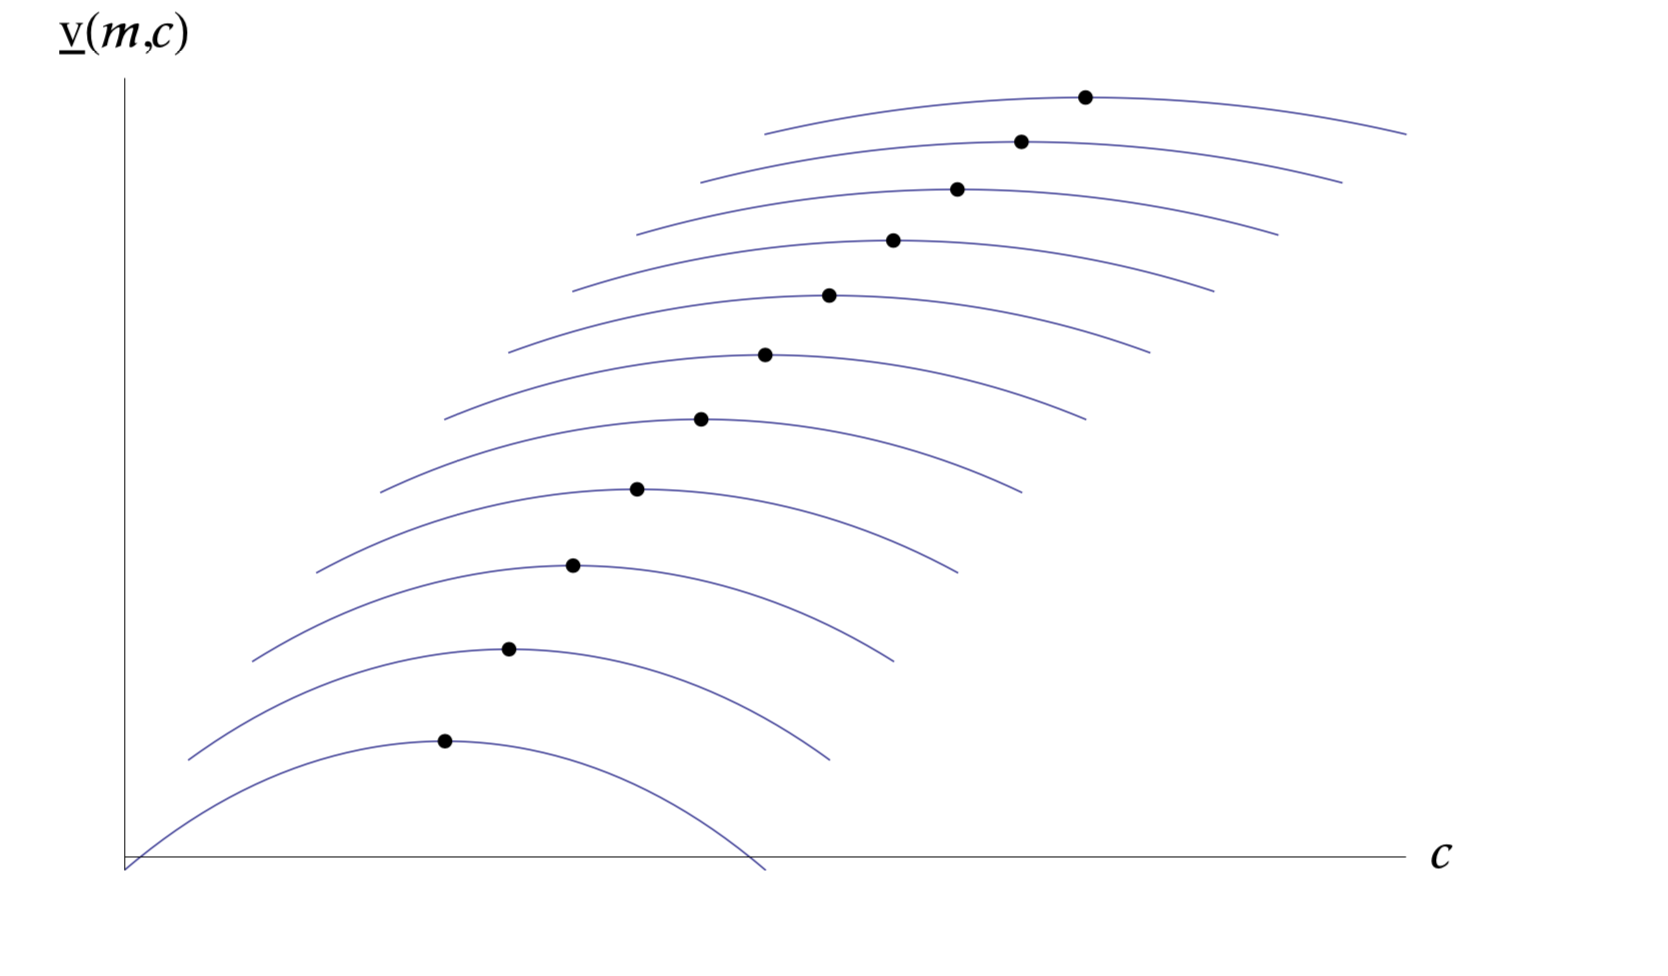
\includegraphics[width=15cm]{./Figures/20180212-envelope-theorem}
  \label{fig:dp-growth-envelope}
%
%  \small{Source: PBOC.}
\end{figure}

%!TEX root = ../DSGEnotes.tex
\chapter{线性二次最优控制}
\label{sec:linear-quardratic-control-intro}
多数情况下,均衡条件较为复杂,无法直接得出解析解。我们需要引入线性二次最优控制理论(optimal linear-quadratic control, LQ),将均衡条件用状态-空间形式表现出来(state-space representation)。这里对线性二次最优控制论问题做简要介绍。

假定一个经济系统,由一系列状态变量的向量$x_t$和一系列控制变量的向量$u_t$构成;$x_t$受到外生随机冲击$\varepsilon_t$的干扰,外生冲击的方差-协方差矩阵为$\sum$。这样一个线性二次最优控制问题可以表述如下:经济系统的决策者通过选择$u_t$来影响$x_t$的走向,由此我们来构建目标方程和状态转移方程。

\section{目标方程和状态转移方程}
目标方程(objective function):
\begin{equation}
  \label{eq:LQC-obj-function}
  \max_{\{u_t\}} E \sum_{t=0}^{\infty} \beta^t \left[ x_t^T R x_t + u_t^T Q u_t\right],
\end{equation}
其中$\beta$是时间贴现系数,对称矩阵$R$和$Q$分别对应目标方程中状态变量和控制变量的权重。

状态转移方程(transition function):
\begin{equation}
  \label{eq:LQC-trans-function}
  x_{t+1}=A x_t + B u_t + \varepsilon_{t+1},
\end{equation}
当期状态由上期状态变量、上期控制变量所共同决定,二者的权重分别由矩阵$A$和$B$所反映。此外,当期状态还受到当期随机冲击的影响,假定是一个Gaussian过程$\{\varepsilon_{t}\}_{t=0}^{\infty} \sim \mathcal{N}(0,\Sigma)$。

\section{价值方程}
在给定时间贴现系数$\beta$的情况下,如果已知系数矩阵$A,B,R,Q$,我们可以求得系统的解。而对于系数矩阵未知的情况,问题则较为复杂。我们引入动态规划(dynamic programming, DP)的思路,定义价值方程$V(x_t)$表示当期状态变量的价值。结合状态转移方程\eqref{eq:LQC-trans-function}和目标方程\eqref{eq:LQC-obj-function},迭代形式表现的价值方程(value function)优化问题如下
\begin{align}
  \label{eq:LQC-value-object}
  V(x_t) &= \max_{\{u_t\}} \left\{
  x_t^T R x_t + u_t^T Q u_t + \beta E[V(x_{t+1})]
  \right\} \nonumber \\
  &=\max_{\{u_t\}} \left\{
  x_t^T R x_t + u_t^T Q u_t + \beta E[V(Ax_{t} + B u_{t} + \varepsilon_{t+1})]
  \right\},
\end{align}
为了求解线性二次最优控制问题  \eqref{eq:LQC-value-object},我们需要两方面信息。一是政策方程(policy function)的具体形式 $u_t = g(x_t)$,即基于当期状态,决策者如何选择最优控制变量,见第\ref{sec:linear-policy-function}节。二是基于当期状态,价值方程的具体形式。

对于后者,方案设计如下:首先我们假设
\begin{equation}
  \label{eq:LQC-value-function}
  V(x_t) = x_t^T P x_t + d,
\end{equation}
即价值方程是关于状态变量的二项式形式(第\ref{sec:LQC-lin-policy-quad-value-impli}节验证价值方程的二项式形式假设是否成立),系数表示为幂等矩阵$P$,满足$P=P^T=P^2$,$d$是个常数矩阵。

随后,将\eqref{eq:LQC-value-function}代回\eqref{eq:LQC-value-object}可得Bellman equation形式的价值方程
\begin{align}
  V(x_t)&=\max_{\{u_t\}} \left\{
  x_t^T R x_t + u_t^T Q u_t + \beta E \left[
  \left(A x_t + B u_t + \varepsilon_{t+1}\right)^T P \left(A x_t + B u_t + \varepsilon_{t+1}\right)  \right] + \beta d
  \right\} \nonumber \\
\label{eq:LQC-value-function-min-problem}
  &\equiv \max_{\{u_t\}} \left\{
  x_t^T R x_t + u_t^T Q u_t + \beta E \left[
  \mathcal{X}  \right] + \beta d
  \right\},
\end{align}
其中
\begin{align*}
  E [\mathcal{X}] = & x_t^T A^T P A x_t + x_t^T A^T P B u_t + u_t^T B^T P A x_t + u_t^T B^T P B u_t \\
  & + \left(x_t^T A^T P \varepsilon_{t+1}  + u_t^T B^T P \varepsilon_{t+1} + \varepsilon_{t+1}^T P A x_t + \varepsilon_{t+1}^T P B u_t \right)+ \varepsilon_{t+1}^T P \varepsilon_{t+1},
\end{align*}
根据定义式$E[\varepsilon] = 0$,上式进一步简化为
\begin{equation}
  \label{eq:LQC-value-function-auxiliary-mathcalX}
  E [\mathcal{X}] =  x_t^T A^T P A x_t + x_t^T A^T P B u_t + u_t^T B^T P A x_t + u_t^T B^T P B u_t + \varepsilon_{t+1}^T P \varepsilon_{t+1}.
\end{equation}

\subsection{一阶条件}
决策者最优行为可由\eqref{eq:LQC-value-function-min-problem}的一阶条件求得
\begin{align}
  \frac{\partial V(x_t)}{\partial u_t} &=\frac{\partial u_t^T Q u_t}{\partial u_t} + \beta \frac{E[\mathcal X]}{\partial u_t} \nonumber \\
  &= \frac{\partial u_t^T Q u_t}{\partial u_t} + \beta \left(
  \frac{\partial x_t^T A^T P B u_t}{\partial u_t} + \frac{\partial u_t^T B^T P A x_t}{\partial u_t} + \frac{u_t^T B^T P B u_t}{\partial u_t} \right) \nonumber \\
  \label{eq:LQC-value-function-FOC}
  &=2Q u_t + 2 \beta B^T P A x_t + 2 \beta B^T P B u_t= 0,
\end{align}
其中为了求得最后一行等式,我们做一些矩阵运算见第\ref{sec:LQC-value-function-FOC-math}节。
\subsubsection{计算一阶条件所需的部分矩阵运算}
\label{sec:LQC-value-function-FOC-math}

对于对称的常系数矩阵$\Gamma$,首先我们有\footnote{这是由于\begin{align*}
  tr(d(u^T \Gamma u)) &= tr(d((u^T \Gamma)(u))) = tr(u^T \Gamma du + d(u^T \Gamma) u) = tr(u^T \Gamma du + d(u^T \Gamma)^T u) \\
  &=tr(u^T \Gamma du) + tr(u^T + d(u^T \Gamma)) = tr(u^T \Gamma du) + tr(u^T \Gamma^T du) = tr(u^T (\Gamma + \Gamma^T) du).
\end{align*}}
\begin{equation*}
  \frac{d}{du}(u^T \Gamma u)= u^T (\Gamma + \Gamma^T) = 2 \Gamma u,
\end{equation*}
于是
\begin{align*}
  &\frac{\partial u_t^T Q u_t}{\partial u_t} = 2 Q u_t, \\
  &\frac{\partial u_t^T B^T P B u_t}{\partial u_t} = 2 B^T P B u_t.
\end{align*}

其次我们有\footnote{这是由于
\begin{equation*}
  tr(d u^T \Gamma) = tr(d(\Gamma^T u)^T) = tr(d (\Gamma^T u)).
\end{equation*}}
\begin{align*}
  &\frac{d}{d u} \Gamma u = \Gamma^T, \\
  &\frac{d}{d u} u^T \Gamma = \Gamma,
\end{align*}
于是
\begin{equation*}
  \frac{\partial x_t^T A^T P B u_t}{\partial u_t} + \frac{\partial u_t^T B^T P A x_t}{\partial u_t} = (x_t^T A^T P B)^T + (B^T P A x_t) = 2 B^T P A x_t.
\end{equation*}

\section{政策方程}
\label{sec:linear-policy-function}
重新整理\eqref{eq:LQC-value-function-FOC},可以得到政策方程$u_t=g(x_t)$的近似线性表达形式
\begin{equation}
  \label{eq:LQC-linear-policy-func}
  u_t = -\left(Q + \beta B^T P B\right)^{-1} \beta B^T P A x_t.
\end{equation}

换句话说,决策者的最优行为可以描述为如下政策方程:
\begin{align}
  \label{eq:LQC-linear-policy-function}
  &u_t = -F x_t, \quad \text{其中}\\
  \label{eq:LQC-linear-policy-F}
  &F = \beta \left(Q + \beta B^T P B \right)^{-1} B^T P A.
\end{align}

基于政策方程\eqref{eq:LQC-linear-policy-function},控制变量$u_t$随着观测到的状态$x_t$做线性调整,调整依据是系数矩阵$F$。$F$的确是一个非线性的函数形式,其值取决于两组矩阵:基础矩阵$A, B, Q$和(假设为二次形式)价值方程中的$P$。一旦我们算出$P$,便可以进一步算出$F$的值,从而求得政策方程的完整形式\footnote{另一种方案是,先求得F,根据F测算出P,如\cite[Ch.2]{Hansen:2004va}}。

\subsection{政策方程满足确定性等价条件}
\label{sec:LQC-policy-function-certainty-equivalence}
政策方程的政策意义价值还在于,它不受外生随机冲击$\varepsilon$的干扰\footnote{除非以下情况出现:如第一,外生冲击彼此相关(所以我们要在模型设定中假设不相关)。第二,目标方程\eqref{eq:LQC-obj-function}并不是二次形式。},这是由于在这样一个线性二次系统中,确定性等价(certainty equivalence)成立,见第\ref{sec:LQC-policy-function-certainty-equivalence}、\ref{sec:LQC-value-function-certainty-equivalence}节。

\section{线性政策方程和二次价值方程}
\label{sec:LQC-lin-policy-quad-value-impli}
如前文所述,线性政策方程
\eqref{eq:LQC-linear-policy-function}-\eqref{eq:LQC-linear-policy-F}
是基于(假设的)二次价值方程
\eqref{eq:LQC-value-function-min-problem}-\eqref{eq:LQC-value-function-auxiliary-mathcalX}
得出的。现在我们反证,基于这样的线性政策方程的确可以得到二次形式的价值方程。一旦反证成功,我们便可以进一步求得$P$和$d$。

将\eqref{eq:LQC-linear-policy-function}代入\eqref{eq:LQC-value-function-min-problem}\footnote{第三个等号所需条件:根据定义$P=P^T$,因此$x_t^T F^T B^T P A x_t$和$x_t^T A^T P B F x_t$都是标量,且满足\begin{equation*}
x_t^T F^T B^T P A x_t = x_t^T A^T P B F x_t.
\end{equation*}}
\begin{align}
  \label{eq:LQC-value-function-min-expand}
  V(x_t) =& x_t^T R x_t + \left(-F x_t\right)^T Q \left(-F x_t\right) + \beta d  + \beta E[\varepsilon_{t+1}^T P \varepsilon_{t+1}] \nonumber \\
  &+\beta E \left[
  x_t^T A^T P A x_t + x_t^T A^T P B \left(-F x_t\right) + \left(-F x_t\right)^T B^T P A x_t + \left(-F x_t\right)^T B^T P B \left(-F x_t\right) \right] \nonumber \\
  =& x_t^T R x_t + x_t^T F^T Q F x_t + \beta d  + \beta E[\varepsilon_{t+1}^T P \varepsilon_{t+1}] \nonumber \\
  &+ \beta E\left[
  x_t^T A^T P A x_t - x_t^T A^T P B F x_t - x_t^T F^T B^T P A x_t + x_t^T F^T B^T P B F x_t \right] \nonumber \\
  =& x_t^T R x_t + x_t^T F^T Q F x_t + \beta E \left[
  x_t^T A^T P A x_t - 2 x_t^T A^T P B F x_t + x_t^T F^T B^T P B F x_t \right] \nonumber \\
  &+ \beta E[\varepsilon_{t+1}^T P \varepsilon_{t+1}] + \beta d.
\end{align}

联立\eqref{eq:LQC-value-function}和\eqref{eq:LQC-value-function-min-expand},我们有
\begin{equation*}
\begin{cases}
  d = \beta E[\varepsilon_{t+1}^T P \varepsilon_{t+1}] + \beta d, \\
  x_t^T P x_t = x_t^T R x_t + x_t^T F^T Q F x_t + \beta E \left[
  x_t^T A^T P A x_t - 2 x_t^T A^T P B F x_t + x_t^T F^T B^T P B F x_t \right].
\end{cases}
\end{equation*}

\subsection{价值方程满足确定性等价条件}
\label{sec:LQC-value-function-certainty-equivalence}
来看第一个等式,整理可得\footnote{这是由于\begin{equation*}
E[\varepsilon_{t+1}^T P \varepsilon_{t+1}] = tr(E[\varepsilon_{t+1}^T P \varepsilon_{t+1}]) = tr(P E[\varepsilon_{t+1}^T \varepsilon_{t+1}]) = tr(P E[\Sigma_{t+1}]).
\end{equation*}}

\begin{equation}
  \label{eq:LQC-value-function-certainty-equivalence}
  d = \frac{\beta}{1-\beta} tr(P \Sigma),
\end{equation}
可见随机冲击$\varepsilon$尽管对价值方程产生影响,但不是通过$F$至政策方程进而影响价值方程,而是通过常数项$d$影响价值方程的。因此,对于最优价值方程而言,确定性等价条件依然成立。

\subsection{代数矩阵Riccati方程}
第二个等式整理,并引入最优政策方程\eqref{eq:LQC-linear-policy-F}替换$F$得\footnote{最后一个等号的计算依据如下:
\begin{align*}
  &\beta A^T P B \left(\left(Q + \beta B^T P B \right)^{-1}\right)^T \left(Q + \beta B^T P B \right) \left(Q + \beta B^T P B \right)^{-1} \beta B^T P A \\
  &=  \beta A^T P B \left(\left(Q + \beta B^T P B \right)^{T}\right)^{-1} \left(Q + \beta B^T P B \right) \left(Q + \beta B^T P B \right)^{-1} \beta B^T P A \\
  &=  \beta A^T P B \left(\left(Q + \beta B^T P B \right)^{T}\right)^{-1} \left(Q + \beta B^T P B \right)^T \left(Q + \beta B^T P B \right)^{-1} \beta B^T P A \\
  &= \beta^2 A^T P B \left(Q + \beta B^T P B \right)^{-1} B^T P A.
\end{align*}
}
\begin{align}
  P =& R + F^T Q F + \beta \cdot \left(A^T P A - 2 A^T P B F + F^T B^T P B F\right) \nonumber \\
  =& R + \beta A^T P A - 2 \beta A^T P B F + F^T \left(Q + \beta B^T P B \right) F \nonumber \\
  =& R + \beta A^T P A - 2 \beta A^T P B \left(Q + \beta B^T P B \right)^{-1} \beta B^T P A \nonumber \\
  + & \beta A^T P B \left(\left(Q + \beta B^T P B \right)^{-1}\right)^T \left(Q + \beta B^T P B \right) \left(Q + \beta B^T P B \right)^{-1} \beta B^T P A \nonumber \\
  \label{eq:LQC-alg-mat-Riccati-equation}
  =& R + \beta A^T P A - \beta^2 A^T P B \left(Q + \beta B^T P B \right)^{-1} \beta B^T P A.
\end{align}

\eqref{eq:LQC-alg-mat-Riccati-equation}又称线性矩阵Riccati方程(linear matrix Riccati equation),它表明价值方程中的$P$是个与基础矩阵$A,B,R,Q$有关的函数,呈非线性关系。

此外,由\eqref{eq:LQC-alg-mat-Riccati-equation}可以看出,一个线性的最优政策方程\eqref{eq:LQC-linear-policy-function}-\eqref{eq:LQC-linear-policy-F},的确预示着二次形式的价值方程  \eqref{eq:LQC-value-function},\eqref{eq:LQC-alg-mat-Riccati-equation}。

\section{数值方法}
在线性二次控制中,在利用解析法推得线性代数Riccati方程后,需要依赖数值计算的方法,对$P$的矩阵Riccati差分方程做迭代近似。假定期初猜测值为$P_{j}$,经过1次迭代,$P_{j+1}$的值更新至
\begin{equation}
  \label{eq:LQC-mat-Riccati-equation-iteration}
  P_{j+1}=R + \beta A^T P_j A - \beta^2 A^T P_j B \left(Q + \beta B^T P B \right)^{-1} \beta B^T P_j A.
\end{equation}

重复迭代,直至$P$收敛到某一值。根据数值模拟的$P$值计算$F$值,进而得到最优政策方程和价值方程。

\section{范例}
假定这样一个线性二次控制问题。中央银行试图通过控制利率$r_t$来影响通货膨胀率$\pi_t$和产出$y_t$,收益方程(payoff function)
\begin{equation}
  \mathcal{L}_t=\pi_t^2 + y_t^2 + 0.1 r_t^2.
\end{equation}

经济系统的结构,由两个状态变量的运动定律构成
\begin{subequations}
  \begin{align}
    \label{eq:LQC-example-pi-motion}
    \pi_{t+1} &= 0.75 \pi_t - 0.5 r_t + \varepsilon_{\pi,t+1}, \\
    \label{eq:LQC-example-y-motion}
        y_{t+1} &= 0.25 y_t - 0.5 r_t + \varepsilon_{y,t+1}.
  \end{align}
\end{subequations}

作为决策者,中央银行的最大化问题为
\begin{equation*}
  \max_{\{r_t\}} E \sum_{t=0}^{\infty} \beta^t \mathcal{L}_t ,\quad \text{ s.t.}     \eqref{eq:LQC-example-pi-motion}-\eqref{eq:LQC-example-y-motion}
\end{equation*}

\subsection{最优线性二次控制问题}
将这一问题改写为最优线性二次控制的一般形式:
\begin{align*}
  \label{eq:LQC-example-LQ-form}
  &\max_{\{u_t\}} E \sum_{t=0}^{\infty} \beta^t \left(x_t^T R x_t + u_t^T Q u_t\right), \\
  &\text{ s.t. } x_{t+1} = A x_t + B u_t + \varepsilon_t,
\end{align*}
其中状态变量,控制变量,外生扰动变量分别用$x_t,u_t,\varepsilon_t$表示
\begin{equation*}
  x_t \equiv \begin{pmatrix}
    \pi_t \\
    y_t
  \end{pmatrix},\quad
  u_t \equiv r_t,\quad
  \varepsilon_t = \begin{pmatrix}
  \varepsilon_{\pi,t} \\
  \varepsilon_{y,t}
  \end{pmatrix},
\end{equation*}
基础系数矩阵$A,B,R,Q$分别为
\begin{equation*}
  A=\begin{pmatrix}
  0.75 & 0 \\
  0 & 0.25
  \end{pmatrix}, \quad
  B = \begin{pmatrix}
  -0,5 \\ -0.5
  \end{pmatrix}, \quad
  R = \begin{pmatrix}
  1 & 0 \\
  0 & 1
  \end{pmatrix}, \quad
  Q=0.1.
\end{equation*}

如前文所述,我们需要使用数值方法,递归处理线性矩阵Riccati方程以近似价值方程系数矩阵$P$,进而测算政策方程的系数矩阵$F$,对应  \eqref{eq:LQC-mat-Riccati-equation-iteration} \eqref{eq:LQC-linear-policy-F}。

%\subsection{Matlab程序说明}
\subsection{Matlab程序}
\begin{lstlisting}[language=Matlab]
clear;
%时间贴现系数的确定
beta = 0.99;

%定义矩阵
R=zeros(2,2);
Q=zeros(1,1);
A=zeros(2,2);
B=zeros(2,1);

%为矩阵赋值
R(1,1)=1;
R(2,2)=1;
Q(1,1)=0.1;
A(1,1)=0.75;
A(2,2)=0.25;
B(1,1)=-0.5;
B(2,1)=-0.5;

%matrix Riccati equation迭代
%d描述$P_j$和邻近迭代$P_{j+1}$之间元素的最大绝对值偏差
d = 1;
%i记录迭代次数
i = 0;
% 最大绝对值偏差d保存在D;迭代次数i保存在I
D=0;
I=0;
%迭代P的初始值定义为P0
%说明:定义P0和Q的非零值,为了使得linear matrix Riccati equation迭代操作中
%$(Q+\beta B^T P_j B) \neq 0$. 只有这个值不等于0,才能使得该矩阵是可逆的。
P0=zeros(2,2);
P0(1,1)=-0.000001;
P0(2,2)=-0.000001;


format long

%matrix Riccati Equation 迭代
%迭代新生成的$P_{j+1}$写入矩阵P1。
%两个P值的差值,写入矩阵Pd。
%当d<0.0000000001时,迭代终止。否则继续进行。
%每次迭代的d和i写入D和I,以备最终程序输出。
while d > 0.0000000001
P1 = R + beta * A' * P0 * A - beta^2 * A' * P0 * B * (inv(Q+beta * B' * P0 * B)) *  (B' * P0 * A);
Pd = P1 - P0;
d = max(abs(Pd));
d = max(d');
D=[D d];
P0 = P1;
i = i+1;
I = [I i];
end

%根据迭代生成的P值,计算policy function的矩阵F
P=P0;
F = -inv(Q + beta * B' * P * B) * (beta * B' * P * A);
ID = [I(2:length(I))' D(2:length(I))'];
disp('       i                         d');
disp(ID);
disp('  SOLUTIONS');
disp('F');
disp(F);
disp('P');
disp(P);
\end{lstlisting}

\subsection{Matlab程序输出}
运行Matlab程序,输出如下
\begin{lstlisting}
  i                         d
1.000000000000000   1.000000938124847
2.000000000000000   0.325234163624664
3.000000000000000   0.080558191789241
4.000000000000000   0.018875706161742
5.000000000000000   0.004338686564976
6.000000000000000   0.000992730600232
7.000000000000000   0.000226907809828
8.000000000000000   0.000051851748175
9.000000000000000   0.000011848232754
10.000000000000000   0.000002707312049
11.000000000000000   0.000000618616947
12.000000000000000   0.000000141352999
13.000000000000000   0.000000032298933
14.000000000000000   0.000000007380254
15.000000000000000   0.000000001686376
16.000000000000000   0.000000000385334
17.000000000000000   0.000000000088048

SOLUTIONS
F
0.744954171236066   0.175909878487998

P
1.430293038776173  -0.106183304364736
-0.106183304364736   1.044189928712962
\end{lstlisting}

由此可得最优政策方程
\begin{align}
  &u_t = - F x_t, \quad r_t = -F \begin{pmatrix} \pi_t \\ y_t \end{pmatrix}, F = (0.745, 0.176)\\
\label{eq:LQC-example-policy-function}
  & r_t = 0.745 \pi_t + 0.176 y_t.
\end{align}

价值方程
\begin{equation}
  \label{eq:LQC-example-value-function}
  V(\pi_t,y_t)= 1.430 \pi_t^2 + 1.044 y_t^2 - 0.212 y_t.
\end{equation}

根据最优政策方程,当通胀水平和/或产出水平高于稳定状态时,中央银行应当提高利率\footnote{注意式中的变量$z_t = (\tilde{z}_t - z)/z$,表示实际观测到的变量,相对于稳态水平的deviation。}。利率对通胀波动的响应幅度高于对产出波动的响应(0.745相对于0.176),这与模型的假设条件有关:
\eqref{eq:LQC-example-pi-motion}-\eqref{eq:LQC-example-y-motion}假定通胀波动比产出波动更为持久(0.75相对于0.25),从而过去时段的物价波动,比起产出波动来,更有可能对当期经济系统产生影响。

根据价值方程,首先同样地,通胀波动二次项的系数大于产出波动二次项的系数。交互项的系数为负,反映了当通胀和产出的波动同方向变化时,比如通货膨胀伴随产出增加(或通货紧缩伴随产出减少),中央银行更容易通过调节利率这一政策工具来稳定经济运行。反之,如果两种波动反方向变化,稳定经济运行将更为困难。

%!TEX root = ../DSGEnotes.tex
\chapter{理性期望模型}
\label{sec:rational-exp-chap}

\section{简介}
利用动态规划(dynamic programming)的方法求解Ramsey随机增长模型,一个核心假定是只存在一个典型的经济行为个体,他追求自身利益最大化的行为带来社会福利最大化。我们称这样的经济体为centralized economy,均衡状态处于Pareto optimality,这个经济行为人称为social planner。

然而现实中更常见decentralized economy的情况,即存在异质的多个经济个体,他们的最大化目标各异,如厂商追求利润最大化,家庭追求效用最大化,劳动者做劳动——休闲的最优决策,等等。的确,根据福利经济学第二定律(the second fundamental theorem of welfare economics, \cite[p.151]{MasColell:1995ue}),在某些极端情况下,完全竞争的decentralized均衡状态可以导致social planner的Pareto optimality;但对于更一般的情况,当decentralized economies中存在局部摩擦如价格/工资粘性时,decentralized均衡并不必然导致centralized的Pareto optimality。换句话说,我们无法通过求解social planner问题来推得decentralized均衡。我们只能直接从不同异质经济个体的一阶条件(FOC)入手,构建这样一组线性随机一阶差分方程,即理性期望模型。

求解理性期望模型的核心在于线性化:在将多阶自回归改写成一阶自回归形式之后,如何将原本是高度非线性的一阶自回归系统做线性近似。对于稍微复杂一些的系统而言,往往无法直接求得解析解,替代方案为:首先将模型变量围绕其稳定状态做对数线性化处理求得解析式;随后根据一定的数值算法,求解线性化方程组,将相关内生变量改写为自VAR形式。

此种求解思路主要来自\cite{King:1988bk, King:1988kf}\footnote{此外可见\cite{King:1999jc}。},大致说来分为四个步骤:
\begin{enumerate}
  \item 计算稳定状态,
  \item 将解释变量围绕稳定状态做近似,求解析式,
  \item 模型参数校准,
  \item 根据数值算法求得政策方程,将内生变量与外生变量和前定变量联系起来。
\end{enumerate}

该思路在宏观经济研究中得到了较为广泛的应用,主要得益于其优点:存在多种可供选择的数值算法,可以在一定程度上近似非线性一阶条件的线性表达式,而只需要付出一定的计算机处理时间。也正因如此,该思路也存在着适用性的局限。
\begin{enumerate}
  \item 围绕稳定状态做对数线性近似,其前提假定是模型接近对数线性形式。而模型非线性的程度越高,模型的规模越大,考虑的因素越是多(比如消费者的风险厌恶程度越高,外生冲击的种类越多),对数线性近似导致的失真情况就越严重。
  \item 稳定状态无法在模型内部求得,并且对于存在多重稳态的经济系统来说,情况会变的更复杂。
\end{enumerate}

\section{数值算法}
针对一阶线性近似的变型系统,常见的数值算法,大致说来有\footnote{一个更为详尽的综述,见\citep{Milani:2012jt}。}
\begin{enumerate}
  \item 特征值——特征向量分解法(eigenvalue-eigenvector decomposition)

  最早由\cite{Blanchard:1980gi}提出,因此也称为Blanchard-Kahn Algorithm。模型要求将所有内生变量分为两类,一类为状态变量,主要指前定变量。其他变量归入第二类跳跃变量(jump variables)。通过特征根——特征变量分解,该算法求得跳跃变量爆炸根(explosive root)的数量,进而判断系统解是否存在,以及是否唯一。见第\ref{sec:simple-BK-algorihtm}节。

  对于满足一些假定条件的(比如非奇异方块矩阵)常规系数矩阵,特征根——特征向量分解法提供了一种较好的求解思路。由此优点出发,在算法方面,一些后续研究作出不断改进
  \citep{King:1998hm, King:2002ko, Anderson:1985hh, Anderson:1998dp, Sims:2002jc, Klein:2000bc, Soderlind:1999kg}。
  \item 未定系数法(undetermined coefficients)

  最早由\cite{McCallum:1983fz}提出,随后的一系列重要扩展包括\cite{Uhlig:1999vx, Binder:1995uf, Christiano:2002uk}等。这种方法不再将变量区分为前定与非前定变量,根据未定系数近似系统的数值解。见第\ref{sec:simple-christiano-undetermined-coefficients}节。

  其基本思路是:第一,假定系统存在1个解,根据这个解,内生变量是关于状态变量的线性方程,并且这个假定不能使完全随机的猜测。第二,将猜测解代回结构方程系统中,构建关于待定系数的方程组。第三,利用二次方程矩阵的解法,求得该方程组的解,进而整个线性系统的解。

  未定系数法具有可操作性和计算速度等优势。但存在不足:第一,需要预先假定模型存在唯一解。第二,仅当系统中没有冗余变量时(系数矩阵的列线性不相关),状态——空间表现形式处于最简规模,该方法才适用。否则值为0的特征值会导致泡沫解的出现\citep[p.57]{Canova:2011vi}。
  \item 期望误差法(expectational errors)

  由\cite{Sims:2002jc}提出,也不再做前定、非前定变量的区分,更可以进一步探讨理性期望下期望误差的性质。见第\ref{sec:simple-sims-expectational-errors}节。

  \item 参数化期望算法(PEA, Parameterised Expectations Algorithm),见第\ref{sec:simple-pea-algorithm}节。

  \item Schur分解法(Schur Decomposition),又称QZ分解法,作为更为通用的形式,主要用于奇异(不可逆)系数矩阵的情况\citep{King:1998hm, King:2002ko, Soderlind:1999kg, Klein:2000bc},见第\ref{sec:simple-schur-decomp}节。

\end{enumerate}

大致说来,各种方法之间的主要区别在于
\begin{itemize}
  \item 构建稳定解模块的方式,
  \item 求解过程中对理性期望的处理,
  \item 保留多大部分的非线性成分,交给数值算法去近似处理,
  \item 对前定和非前定变量的区分等。
\end{itemize}

根据\cite{King:1988bk, King:1988kf}的四步骤求解思路,第\ref{sec:simple-sto-grow-model}节首先建立一个简单的随机增长模型。在此基础上,第\ref{sec:simple-steady-state}节计算稳定状态,第\ref{sec:simple-loglin}节做对数线性化近似,第\ref{sec:simple-BK-algorihtm}-\ref{sec:simple-schur-decomp}节分别介绍几种主要的算法。

\section{一个简单的随机增长模型}
\label{sec:simple-sto-grow-model}
在这样一个简单随机经济增长模型中,典型个体追求最大化问题
\begin{align*}
  & \max_{\{C_t\}} E \sum_{t=0}^{\infty} \beta^t \cdot \left(\frac{C_t^{1-\sigma}}{1-\sigma}\right), \quad \text{s.t.} \\
& C_t + K_{t+1} = A_t \cdot K_{t}^{\alpha} + (1-\delta) \cdot K_{t}, \\
& \ln A_t = \rho \cdot \ln A_{t-1} + \varepsilon_t, , \quad \varepsilon_{t} \sim i.i.d. (0, \sigma^2), 0<\rho < 1.
\end{align*}
模型的均衡解以$\{C_t,K_t,Y_t\}_{t=0}^{\infty}$的形式展现。

求解一阶条件我们有
\begin{equation*}
  \begin{cases}
    C_t^{-\sigma} &= \beta E \left[
    C_{t+1}^{-\sigma} \cdot \left(\alpha \cdot A_{t+1} \cdot K_{t+1}^{\alpha - 1} + 1 - \delta \right)
    \right] \\
    C_t + K_{t+1} &= A_t \cdot K_t^{\alpha} + (1-\delta) \cdot K_t \\
    \ln A_t &= \rho \cdot \ln A_{t-1} + \varepsilon_t
  \end{cases}
\end{equation*}

\subsection{稳定状态}
\label{sec:simple-steady-state}
在稳定状态下我们有
\begin{equation*}
  \begin{bmatrix}
    C_t \\
    K_t \\
    Y_t
  \end{bmatrix} \equiv
  \begin{bmatrix}
    \bar{C} \\
    \bar{K} \\
    \bar{Y}
    \end{bmatrix}, \quad A_t \equiv \bar{A} = 1, \quad \forall t.
\end{equation*}

进而我们有
\begin{equation*}
  \begin{cases}
    1 &= \beta \cdot \left[
    \alpha \cdot \bar{K}^{\alpha - 1} + (1-\delta)
    \right], \\
    \bar{C}+ \bar{K} &= \bar{K}^{\alpha} + (1-\delta) \cdot \bar{K}.
  \end{cases}
\end{equation*}

整理后得稳定状态
\begin{equation*}
  \begin{cases}
    \bar{C} &= \bar{K}^{\alpha} - \delta \cdot \bar{K}, \\
    \bar{K} &= \left(
    \frac{1-(1-\delta) \cdot \beta}{\alpha \cdot \beta}
    \right)^{\frac{1}{\alpha - 1}}, \\
    \bar{Y} &= \bar{K}^{\alpha}.
  \end{cases}
\end{equation*}

\subsection{对数线性化}
\label{sec:simple-loglin}
对数线性的定义式可表示为,对于一个变量$X_t$:
\begin{equation*}
%  \label{eq:simple-log-lin-def}
  \tilde{X_t} \equiv \frac{X_t - \bar{X}}{\bar{X}} \approx \ln X_{t} - \ln \bar{X},
\end{equation*}

对于含有不止一个变量的复杂方程$f(X_t,Y_t)$,对其稳定状态$(\bar{X}, \bar{Y})$做一阶泰勒级数展开的方式为
\begin{equation*}
  \ln f(X_t,Y_t) \approx \ln f(\bar{X}, \bar{Y}) + \left[\frac{
  \frac{\partial f(X_t,Y_t)}{\partial X_t} |_{\{\bar{X},\bar{Y}\}}
  }{f(\bar{X},\bar{Y})}\right] \cdot \left(X_t - \bar{X}\right) +
  \left[\frac{
  \frac{\partial f(X_t,Y_t)}{\partial Y_t} |_{\{\bar{X},\bar{Y}\}}
  }{f(\bar{X},\bar{Y})}\right] \cdot \left(Y_t - \bar{Y}\right).
\end{equation*}

\subsubsection{外生技术冲击的对数线性化}
\begin{equation}
  \label{eq:simple-steady-state-tech-shock}
  \tilde{A}_{t} \approx \rho \cdot \tilde{A}_{t-1} + \varepsilon_t.
\end{equation}

\subsubsection{Euler equation的对数线性化}
等式两侧取对数
\begin{equation*}
  -\sigma \cdot \ln C_t = \ln \beta - \sigma \cdot E \ln C_{t+1} + E  \ln \left[\alpha \cdot A_{t+1} \cdot K_{t+1}^{\alpha - 1} + \left(1 - \delta \right)\right]
\end{equation*}

RHS第三部分,围绕$\{\bar{K}, \bar{A}\}$做一阶泰勒展开
\begin{equation*}
\begin{split}
  &\ln \left[\alpha \cdot A_{t+1} \cdot K_{t+1}^{\alpha - 1} + \left(1 - \delta \right)\right] \\
  & \approx \ln \left[\alpha \bar{A} \bar{K}^{\alpha - 1} + (1-\delta) \right]\\
  &+ \frac{
  \frac{\partial}{\partial \bar{K}} \left[\alpha \cdot \bar{A} \cdot \bar{K}^{\alpha - 1} + (1-\delta) \right] \cdot \frac{K_{t+1} - \bar{K}}{\bar{K}} \cdot \bar{K}
  }
  {
  \alpha \cdot \bar{A} \cdot \bar{K}^{\alpha - 1} + (1-\delta)
  }
  + \frac{
  \frac{\partial}{\partial \bar{A}} \left[\alpha \cdot \bar{A} \cdot \bar{K}^{\alpha - 1} + (1-\delta) \right] \cdot \frac{A_{t+1} - \bar{A}}{\bar{A}} \cdot \bar{A}
  }
  {
  \alpha \cdot \bar{A} \cdot \bar{K}^{\alpha - 1} + (1-\delta)
  } \\
  &= \ln \left[\alpha \cdot \bar{A} \cdot \bar{K}^{\alpha - 1} + (1-\delta) \right] + \frac{
  \alpha \cdot \bar{A} \cdot (\alpha - 1) \cdot \bar{K}^{\alpha - 1} \cdot \tilde{K}_{t+1}
  + \alpha \cdot \bar{K}^{\alpha - 1} \cdot \bar{A} \cdot \tilde{A}_{t+1}
  }{
  \alpha \cdot \bar{A} \cdot \bar{K}^{\alpha - 1} + (1-\delta)
  } \\
  &= \ln \left[ \alpha \cdot \bar{A} \cdot \bar{K}^{\alpha - 1} + (1-\delta) \right]+ \frac{
  \alpha \cdot \bar{K}^{\alpha -1} \cdot \left[ (\alpha - 1) \cdot \tilde{K}_{t+1} + \tilde{A}_{t+1}\right]
  }{\alpha \cdot \bar{A} \cdot \bar{K}^{\alpha - 1} + (1-\delta)} \\
  &= -\ln \beta + \left[1 - \beta \cdot (1-\delta)\right] \cdot \left[ (\alpha - 1) \cdot \tilde{K}_{t+1} + \tilde{A}_{t+1} \right],
\end{split}
\end{equation*}
进而我们有
\begin{equation}
  \label{eq:simple-steady-state-euler}
  -\sigma \cdot \tilde{C}_{t} = -\sigma \cdot \tilde{C}_{t+1} + \left[1 - \beta \cdot (1-\delta) \right] \cdot \left[ (\alpha - 1) \cdot \tilde{K}_{t+1} + \tilde{A}_{t+1}\right]
\end{equation}

\subsubsection{预算约束条件的对数线性化}
等式两侧取对数
\begin{equation*}
  \ln (C_t + K_{t+1}) = \ln \left[ A_t \cdot K_t^{\alpha} + (1-\delta) \cdot K_t\right]
\end{equation*}

LHS $\Rightarrow$
\begin{align*}
  \ln (C_t + K_{t+1}) \approx \ln \left(\bar{C} + \bar{K} \right) + \frac{
  \frac{C_t - \bar{C}}{\bar{C}} \cdot \bar{C} + \frac{K_{t+1} - \bar{K}}{\bar{K}} \cdot \bar{K}
  }{\bar{C}+\bar{K}} = \ln \left(\bar{C} + \bar{K} \right) + \frac{\bar{C} \cdot  \tilde{C}_{t} + \bar{K} \cdot \tilde{K}_{t+1} }{\bar{C}+\bar{K}}.
\end{align*}

RHS $\Rightarrow$
\begin{align*}
  &\ln \left[ A_t \cdot K_t^{\alpha} + (1-\delta) \cdot K_t\right] \\ & \approx \ln \left[ \bar{A} \cdot \bar{K}^{\alpha} + (1-\delta) \cdot \bar{K} \right] + \frac{
  \frac{\partial }{\partial \bar{K}} \left[\bar{A} \bar{K}^{\alpha} + (1-\delta) \cdot \bar{K}\right] \cdot \frac{K_t - \bar{K}}{\bar{K}} \cdot \bar{K}
  }{\bar{A} \cdot \bar{K}^{\alpha} + (1-\delta) \cdot \bar{K} } +
  \frac{
  \frac{\partial }{\partial \bar{A}} \left[\bar{A} \bar{K}^{\alpha} + (1-\delta) \cdot \bar{K}\right] \cdot \frac{A_t - \bar{A}}{\bar{A}} \cdot \bar{A}
  }{\bar{A} \cdot \bar{K}^{\alpha} + (1-\delta) \cdot \bar{K} }\\
  &= \ln \left[ \bar{A} \cdot \bar{K}^{\alpha} + (1-\delta) \cdot \bar{K} \right] + \frac{
  \left[ \alpha \cdot \bar{A} \cdot \bar{K}^{\alpha} + (1-\delta) \cdot \bar{K} \right] \cdot \tilde{K}_{t} + \bar{A} \cdot \bar{K}^{\alpha} \cdot \tilde{A}_{t}
  }{
  \bar{A} \cdot \bar{K}^{\alpha} + (1-\delta) \cdot \bar{K}
  } \\
  &=\ln \left[ \bar{A} \cdot \bar{K}^{\alpha} + (1-\delta) \cdot \bar{K}\right]+ \frac{\frac{1}{\beta} \cdot \bar{K} \cdot \tilde{K}_t + \bar{A} \cdot \bar{K}^{\alpha} \cdot \tilde{A}_t}{
  \bar{A} \cdot \bar{K}^{\alpha} + (1-\delta) \cdot \bar{K}
  } \\
  &= \ln \left(
  \bar{C}+\bar{K}
  \right) +
  \frac{
  \frac{1}{\beta} \cdot \bar{K} \cdot \tilde{K}_t + \bar{K}^{\alpha} \cdot \tilde{A}_t
  }{\bar{C}+\bar{K}}.
\end{align*}

$LHS=RHS \Rightarrow$
\begin{equation*}
  \bar{C} \cdot \tilde{C}_{t} + \bar{K} \cdot \tilde{K}_{t+1} = \frac{1}{\beta} \cdot \bar{K} \cdot  \tilde{K}_{t} + \bar{K}^{\alpha} \cdot \tilde{A}_t,
\end{equation*}

因此我们有
\begin{equation}
  \label{eq:simple-steady-state-budget}
  \begin{split}
  \tilde{K}_{t+1} &= -\frac{\bar{C}}{\bar{K}} \cdot \tilde{C}_t + \frac{1}{\beta} \cdot \tilde{K}_{t} + \bar{K}^{\alpha -1} \cdot \tilde{A}_{t}\\
  &=-\frac{1-\beta \cdot \left[1-\delta \cdot (1-\alpha) \right]}{\alpha \cdot \beta} \cdot \tilde{C}_{t}+\frac{1}{\beta} \cdot \tilde{K}_{t} + \frac{1-\beta \cdot (1-\delta)}{\alpha \cdot \beta} \cdot \tilde{A}_{t}.
  \end{split}
\end{equation}

\subsection{状态——空间表现形式}
\label{sec:simple-state-space-form}
一阶差分式\eqref{eq:simple-steady-state-tech-shock}、\eqref{eq:simple-steady-state-euler}、\eqref{eq:simple-steady-state-budget}共同描述这样一个动态的经济系统$\{ C_t, K_t, A_t\}_{t=0}^{\infty}$。可以将其改写为如下状态——空间表现形式(state-space representation)
\begin{equation}
  \label{eq:simple-state-space-rep}
\begin{bmatrix}
  1 & 0 & 0\\
  0 & 1 & 0\\
  0 & 0 & \sigma
\end{bmatrix}
E
\begin{bmatrix}
  \tilde{A}_{t+1} \\
  \tilde{K}_{t+1} \\
  \tilde{C}_{t+1}
\end{bmatrix} =
\begin{bmatrix}
  \rho & 0 & 0 \\
  \frac{1-\beta \cdot (1-\delta)}{\alpha \cdot \beta} &
  \frac{1}{\beta} &
  -\frac{1-\beta \cdot \left[1-\delta \cdot (1-\alpha) \right]}{\alpha \cdot \beta} \\
  \rho \cdot \left[1 - \beta \cdot (1-\delta)\right] &
  -\left( 1-\alpha \right) \cdot \left[1 - \beta \cdot (1-\delta)\right] &
  \sigma
\end{bmatrix}
\begin{bmatrix}
  \tilde{A}_{t} \\
  \tilde{K}_{t} \\
  \tilde{C}_{t}
\end{bmatrix}.
\end{equation}

\section{特征值——特征方程分解法}
\label{sec:simple-BK-algorihtm}

\subsection{特征值——特征方程分解法}
根据Blanchard-Kahn算法,要将经济系统中的$p+m+k$个变量分类。一类是$k$个外生变量$z_t$。一类是内生变量$x_t$。内生变量再分为$m$个控制变量(跳跃变量)$x_t^j$和$p$状态变量(前定变量)$x_t^s$。\eqref{eq:simple-state-space-rep}可以改写为
\begin{equation}
  \label{eq:simple-KBA-tau}
  \mathcal{T}_0 E x_{t+1} = \mathcal{T}_1 x_t + \Psi z_t, \quad x_t \equiv \left[x_t^s \quad x_t^j \right]'.
\end{equation}

假定系数矩阵$\mathcal{T}_0$是可逆的,上式进一步调整为
\begin{align}
  \label{eq:simple-BKA-matrix-AB}
%  \begin{split}
    &E x_{t+1} = A x_{t} + B z_t, \quad \text{其中}
    A \equiv \mathcal{T}_0^{-1} \mathcal{T}_1, \quad B \equiv \mathcal{T}_{0}^{-1} \Psi, \quad \text{或者} \nonumber \\
    & E \begin{bmatrix}
    \underset{p \times 1}{x_{t+1}^s} \\
    \underset{m \times 1}{x_{t+1}^j}
  \end{bmatrix} = \begin{bmatrix}
  \underset{p \times p}{A_{11}} &
  \underset{p \times m}{A_{12}} \\
  \underset{m \times p}{A_{21}} &
  \underset{m \times m}{A_{22}}
  \end{bmatrix}
  \begin{bmatrix}
  \underset{p \times 1}{x_{t}^s} \\
  \underset{m \times 1}{x_{t}^j}
\end{bmatrix}
+ \begin{bmatrix}
\underset{p \times k}{B_{1}} \\
\underset{m \times k}{B_{2}}
\end{bmatrix}
\underset{k \times 1}{z_t}
%  \end{split}
\end{align}

Blanchard-Kahn算法的核心就在于,对系数矩阵$A$做Jordan decomposition。对于可对角化(diagonalizable)的系数矩阵$A$,假定其特征向量是序列不相关的\footnote{对于n个长度为m的向量之间线性不相关,是指对于由这n个向量构成的$mxn$矩阵$X$来说,$det(x) \neq 0$。},我们有$A P = P \Lambda$,改写为Jordan canonical form
\begin{equation}
  \label{simple-BKA-jordan}
    A = P \Lambda P^{-1},
\end{equation}
其中$\Lambda$是对角矩阵,对角元素对应特征根$\Lambda_{ii} = \lambda_i$,其他元素均为$0$。$P$的每一列为对应$\lambda_i$的特征向量。我们用$\bar{p}$和$\bar{m}$来表示用稳定和不稳定特征根来为矩阵分块的情况,后面会简要探讨当$\bar{p} \neq p, \bar{m} \neq m$时可能会出现的问题,见第\ref{sec:simple-BKA-exist-unique}节。

根据Blanchard-Kahn条件,不稳定特征根(即$|\lambda|>1$)的数量应该恰好等于经济系统中控制变量的数量,以确保相图中鞍点稳定性的存在。如果不稳定特征根的数量少于控制变量的数量,经济系统超稳定,出现未定问题(indeterminacy)\footnote{对未定经济系统问题的探讨,可见如\cite{Benhabib1999}。}。如果多于,经济系统爆炸性发展,会违反横截条件。一个较为详细的讨论见第\ref{sec:simple-BKA-exist-unique}节。

在本章的动态Ramsey经济模型中,内生变量是二维的,由一个控制变量和一个前定状态变量构成。因此需要恰好有一个不稳定特征根和一个稳定特征根。

将特征矩阵做进一步的分解,根据特征根绝对值从低到高做重新排列(相应地,需要调整特征矩阵的列)
\begin{equation*}
%  \label{simple-BKA-eigenvalue-decomp}
  \Lambda = \begin{bmatrix}
  \underset{\bar{p} \times \bar{p}}{\Lambda_{s}} & \underset{\bar{p} \times \bar{m}}{0} \\
  \underset{\bar{m} \times \bar{p}}{0} & \underset{\bar{m} \times \bar{m}}{\Lambda_{e}}
\end{bmatrix}, \quad P = \begin{bmatrix}
P_{11} & P_{12} \\
P_{21} & P_{22}
\end{bmatrix}.
\end{equation*}
其中对角矩阵$\Lambda_s$($\Lambda_e$)的对角元素是绝对值小于(大于)$1$的特征根。系统\eqref{eq:simple-BKA-matrix-AB}由此改写为
\begin{equation}
  \label{eq:simple-BKA-matrix-wz}
  E w_{t+1} = \Lambda w_{t} + \bar{B} z_t, \quad \text{其中} w_t \equiv P^{-1}x_t, \bar{B} \equiv P^{-1} B.
\end{equation}

对应地我们有
\begin{equation*}
  w_t = \begin{bmatrix}
  \underset{\bar{p} \times 1}{w_{1,t}} \\
  \underset{\bar{m} \times 1}{w_{2,t}}
\end{bmatrix}, \quad \bar{B} = \begin{bmatrix}
  \underset{\bar{p} \times \bar{k}}{\bar{B}_{1}}\\
  \underset{\bar{m} \times {k}}{\bar{B}_{2}}
\end{bmatrix}.
\end{equation*}


根据上述分析,由\eqref{eq:simple-BKA-matrix-wz}我们有
\begin{subequations}
  \begin{align}
    \label{eq:simple-BKA-wsz}
    E w_{1,t+1} &= \Lambda_s w_{1,t} + \bar{B}_1 z_t, \\
    E w_{2,t+1} &= \Lambda_e w_{2,t} + \bar{B}_{2} z_t.
    \label{simple-BKA-wez}
  \end{align}
\end{subequations}

根据模型设定,\eqref{eq:simple-BKA-wsz}总是稳定的,因为$\Lambda_s$的对角元素由绝对值小于1的特征根构成。\eqref{simple-BKA-wez}是爆炸的,因为$\Lambda_e$的对角元素由绝对值大于1的特征根构成。因此我们先来考察\eqref{simple-BKA-wez}成立需要满足的条件。

%\eqref{simple-BKA-wez}成立的条件只能是$w_{2,t} = 0$。下面
我们对$w_{2,t}$做forward-looking迭代,求解等式。
%\subsubsection{Forward-looking迭代}
\eqref{simple-BKA-wez}意味着
  \begin{align*}
    w_{2,t} &= (\Lambda_e)^{-1} E w_{2,t+1} - \bar{B}_{2} z_t, \\
    w_{2,t+1} &= (\Lambda_e)^{-1} E w_{2,t+2} - \bar{B}_{2} z_{t+1},\\
    &\vdots \\
    w_{2,t+T} &= (\Lambda_e)^{-1} E w_{2,t+T} - \bar{B}_{2} z_{t+T}.
  \end{align*}

根据forward-looking迭代我们有
\begin{equation}
  w_{2,t} = \lim_{T \rightarrow \infty} \Lambda_e^{-T} E (w_{2,t+T}) - \sum_{s=0}^{T} \Lambda_{e}^{-s-1} \bar{B}_2 E(z_{t+s}).
\end{equation}

由于$\Lambda_{e}$中所有对角元素绝对值都大于$1$,对于$T \rightarrow \infty$可得$\Lambda_{e}^{T} \rightarrow 0$,因此改写上式,$w_{2,t}$的值可以计算如下
\begin{equation}
  \label{eq:simple-BKA-forward-looking-iteration-w}
    w_{2,t} = - \sum_{s=0}^{T} \Lambda_{e}^{-s-1} \bar{B}_2 E(z_{t+s}).
\end{equation}

回到反映$w_t$和$x_t$关系的\eqref{eq:simple-BKA-matrix-wz}中,根据定义
\begin{equation*}
  x_t \equiv P w_t  \Rightarrow \begin{bmatrix}
  \underset{\bar{p} \times 1}{x_{1,t}} \\
  \underset{\bar{m} \times 1}{x_{2,t}}
\end{bmatrix} = \begin{bmatrix}
  P_{11} & P_{12} \\
  P_{21} & P_{22}
\end{bmatrix} \begin{bmatrix}
\underset{\bar{p} \times 1}{w_{1,t}} \\
\underset{\bar{m} \times 1}{w_{2,t}}
\end{bmatrix},
\end{equation*}
等价于
\begin{subequations}
\begin{align}
  \label{eq:simple-BKA-xwp-1}
  x_{1,t} &= P_{11} w_{1,t} + P_{12} w_{2,t}, \\
  \label{eq:simple-BKA-xwp-2}
  x_{2,t} &= P_{21} w_{1,t} + p_{22} w_{2,t}.
\end{align}
\end{subequations}

如果假定$\bar{p}=p, \bar{m}=m$,即系统中控制变量的数量等于不稳定特征根的数量,并且假定$P_{11}$是可逆分块矩阵,则$x_{1,t}=x_t^s, x_{2,t}=x_t^j$,对于二者不相等的情况,见第\ref{sec:simple-BKA-exist-unique}节。对于最终形成Blanchard-Kahn算法的求解思路:
\begin{enumerate}
\item 从初始状态$t=0$出发,对应给定的$x_{t=0}^s$。
\item 结合生成的$z_t$,根据\eqref{eq:simple-BKA-forward-looking-iteration-w}计算$w_{2,t}$:
\begin{equation*}
  w_{2,t} = - \sum_{s=0}^{T} \Lambda_{e}^{-s-1} \bar{B}_2 E(z_{t+s}).
\end{equation*}

\item 根据\eqref{eq:simple-BKA-xwp-1}得到$w_{1,t}$的值:
\begin{equation*}
  w_{1,t} = P_{11}^{-1} x_{t}^s - P_{11}^{-1} P_{12} w_{2,t},
\end{equation*}
其中前定变量$x_t^s$由上一期的状态求得。

\item 根据\eqref{eq:simple-BKA-xwp-2}得到控制变量$x_{t}^j$的值,又称政策方程:
\begin{equation*}
  x_t^j = P_{21} w_{1,t} + P_{22} w_{2,t}.
\end{equation*}

\item 根据 \eqref{eq:simple-BKA-matrix-AB}得到$t+1$期状态变量的期望值$x_{t+1}^s$:
\begin{equation*}
  E x_{t+1}^s = A_{11} x_{t}^s + A_{12} x_{t}^j + B_1 z_t,
\end{equation*}

\item 重复以上步骤。
\end{enumerate}

\subsection{解的存在性以及唯一性}
\label{sec:simple-BKA-exist-unique}
如前文所述,当$p=\bar{p},m=\bar{m}$时,控制变量(状态变量)的数量等于爆炸(稳定)特征根的数量,此时系统均衡解存在且唯一。

但当$m<\bar{m}$时,$p>\bar{p}$,情况有所不同。我们仍然可以根据\eqref{eq:simple-BKA-xwp-1}得到$w_{1,t}$的值,尽管$w_{1,t}$的值不唯一。但在根据\eqref{eq:simple-BKA-xwp-2}测算$x_{t}^j$时,会受到较大限制,比如在$t=0$时:
\begin{equation*}
x_{2,t_0} = P_{21} w_{1,t_0} + p_{22} w_{2,t_0},
\end{equation*}
此时,$x_{2,t_0}$的$\bar{m}$行中,最上面的$\bar{m} - m \equiv p - \bar{p}$行是状态变量,因此是提前给定的。这意味着我们没有足够数量的前定(状态)变量用于求解方程。换句话说,对整个经济系统而言,当跳跃变量的数量少于爆炸特征根时,系统的均衡解不存在。

当$m>\bar{m}$时,$p<\bar{p}$,在$t=0$时\eqref{eq:simple-BKA-xwp-1}变为
\begin{equation*}
  w_{1,t_0}=P_{11}^{-1}x_{1,t_0}-P_{11}^{-1}P_{12}w_{2,t_0},
\end{equation*}
$x_{1,t_0}$的$\bar{p}$行中,最下面的$\bar{p}-p \equiv m - \bar{m}$行是跳跃变量,这会导致解出的$w_{1,t}$并不唯一。这意味着我们可以随意选择这$\bar{p}-p$行跳跃变量的初始值。换句话说,对整个经济系统而言,当跳跃变量的数量多于爆炸特征根时,系统可能存在无数个均衡解。

\subsection{应用Blanchard-Kahn算法实例}
以随机Ramsey增长模型\eqref{eq:simple-state-space-rep}为例,$z_t \equiv \tilde{A}_t, x_t^j \equiv \tilde{C}_t, x_t^s \equiv \tilde{K}_t$,
\begin{equation*}
\begin{bmatrix}
  1 & 0 \\
  (1-\alpha) \cdot [1-\beta \cdot (1-\delta)] & \sigma
\end{bmatrix}
E
\begin{bmatrix}
  \tilde{K}_{t+1} \\
  \tilde{C}_{t+1}
\end{bmatrix}
= \begin{bmatrix}
\frac{1}{\beta} & -\frac{1-\beta \cdot \left[1-\delta \cdot (1-\alpha) \right]}{\alpha \cdot \beta} \\
0 & \sigma
\end{bmatrix}
\begin{bmatrix}
  \tilde{K}_{t} \\
  \tilde{C}_{t}
\end{bmatrix} +
\begin{bmatrix}
  \frac{1-\beta \cdot (1-\delta)}{\alpha \cdot \beta} \\
  \rho \cdot \left[ 1-\beta \cdot (1-\delta) \right]
\end{bmatrix}
\tilde{A}_t。
\end{equation*}

在Matlab中,首先定义系数$\beta, \alpha, \sigma, \delta, \rho$的值。
\begin{lstlisting}[language=matlab,frame=single]
  clear;

  %参数设定
  beta = 0.9;
  alpha = 0.75;
  sigma = 1;
  delta = 0.3;
  rho = 0.95;

\end{lstlisting}

进而计算稳定状态。
\begin{lstlisting}[language=matlab,frame=single]
  %稳态值
  kbar = ((1-(1-delta)*beta)/(alpha * beta))^(1/(alpha - 1));
  cbar = kbar^alpha - delta * kbar;
  ybar = kbar^alpha;
\end{lstlisting}
根据测算结果,$\bar{K}=11.0766, \bar{C} = 2.7486, \bar{Y} = 6.0716$。

输入矩阵$\mathcal{T}_0, \mathcal{T}_1, \mathcal{T}_2$:
\begin{lstlisting}[language=matlab, frame=single]
  %定义矩阵T0,T1,PSI
  Tau0=zeros(2,2);
  Tau1=zeros(2,2);
  Psi=zeros(2,1);
  Tau0(1,1)=1;
  Tau0(1,2)=0;
  Tau0(2,1)=(1-alpha) * (1-beta * (1-delta));
  Tau0(2,2)=sigma;
  Tau1(1,1)=1/beta;
  Tau1(1,2)=-(1-beta * (1-delta * (1-alpha)))/(alpha * beta);
  Tau1(2,1)=0;
  Tau1(2,2)=sigma;
  Psi(1,1)=(1-beta * (1-delta))/(alpha * beta);
  Psi(2,1)=rho * (1-beta * (1-delta));
\end{lstlisting}
Matlab测算出的矩阵值如下:
\begin{equation*}
  \mathcal{T}_0 = \begin{bmatrix}
  1.0000 &       0.0000 \\
  0.0925 &  1.0000
  \end{bmatrix},\quad
  \mathcal{T}_1=\begin{bmatrix}
  1.1111&   -0.2481 \\
  0.0000&    1.0000
  \end{bmatrix}, \quad
  \Psi = \begin{bmatrix}
  0.5481 \\
  0.3515
  \end{bmatrix}.
\end{equation*}

计算$A$和$B$:
\begin{lstlisting}[language=matlab, frame=single]
  %计算矩阵A,B
  A=zeros(2,2);
  B=zeros(2,2);
  A = inv(Tau0) * Tau1;
  B = inv(Tau0) * Psi;
\end{lstlisting}
测算结果:
\begin{equation*}
  A=\begin{bmatrix}
  1.1111 &  -0.2481 \\
  -0.1028 &   1.0230
\end{bmatrix}, \quad B = \begin{bmatrix}
0.5481 \\
   0.3008
\end{bmatrix}.
\end{equation*}

测算$A$的特征值和特征向量:
\begin{lstlisting}[language=matlab, frame=single]
%对A做Jordan decomposition,
%分解为特征值和特征向量
%对A做Jordan decomposition,
%分解为特征值和特征向量
[VE, Lambda] = eig(A); %MU储存特征值
P=inv(VE); %P储存normalized特征向量
\end{lstlisting}
特征值和特征向量如下:
\begin{equation*}
  P=\begin{bmatrix}
    0.7049&   -0.8340 \\
    0.4805&    0.9806
  \end{bmatrix}, \quad \Lambda = \begin{bmatrix}
  1.2327    &     0 \\
     0    & 0.9014
  \end{bmatrix},
\end{equation*}
不难看出,$\lambda_{i},i=(1,2)$分别是不稳定和稳定的特征根,满足Blanchard-Kahn条件,系统是鞍点稳定的。

将特征根矩阵沿着对角线元素(特征根)从低到高的顺序排列。

\todo{to be finished...}


\section{未定系数法}
\label{sec:simple-christiano-undetermined-coefficients}
根据\cite{Christiano:2002uk},假定经济模型以这样的状态——空间形式表现

\begin{equation}
  \label{eq:simple-christiano-state-space}
  \begin{split}
    &\alpha_0 E x_{t+1} + \alpha_1 \cdot x_t + \alpha_2 \cdot x_{t-1} + \beta \cdot z_t = 0, \quad t \ge 0, \\
    &z_t = R \cdot z_{t-1} + \varepsilon_t,
  \end{split}
\end{equation}
其中
\begin{itemize}
  \item $\underset{n \times n}{x_{t}} \Rightarrow$ 在$t$时间决定的内生变量向量,$x_{-1}$是提前给定的。
  \item $\underset{k \times 1}{z_t} \Rightarrow$ 外生技术冲击变量的向量,满足$\varepsilon_{t} \sim i.i.d.(0,\Sigma)$。
  \item 系数矩阵$\underset{n \times n}{\alpha_0}, \underset{n \times n}{\alpha_1}, \underset{n \times n}{\alpha_2}, \underset{n \times k}{\beta}, \underset{k \times k}{R}$。
\end{itemize}

与第\ref{sec:simple-BK-algorihtm}节的Blanchard-Kahn法相比,未定系数法不再将内生变量做状态变量和跳跃变量的区分。好处是让算法(看起来)简化,但这种简化有一定的额外成本:需要预设全部状态变量的初始值$x_{t=0}$(与之相比,Blanchard-Kahn算法则只需要$x_{t=0}^s$):如果初始时间的经济系统恰好完全处于稳定状态,这是没问题的;否则便只能针对每一个均衡方程,分别设定其对应变量的初始条件。

\eqref{eq:simple-christiano-state-space}描述了这样一个经济系统,系统解表现为一个反馈机制:当前内生向量$x_t$与上期$x_{t-1}$和当期外生冲击$z_t$线性相关,因此假定下式
\begin{equation}
  \label{eq:simple-christiano-state-space-AB}
  x_t = \underset{n \times n}{A} \cdot x_{t-1} + \underset{n \times k}{B} \cdot z_{t},
\end{equation}
在静态均衡条件下我们有$z_{t} \equiv 0 \quad \forall t$,这要求系数矩阵$A$的所有特征值绝对值都小于$1$\footnote{回忆一下Blanchard-Kahn算法中将内生变量分为状态和跳跃两部分;对应相同数量的系数矩阵稳定根和不稳定根。未定系数法中所有内生变量$x_t$都是在$t$期决定的,这使得我们不再有多余的自由度用于处理不稳定根。}。现在目标变成了,对于给定的初始值$x_{-1}$,找到系数矩阵$A,B$,使  \eqref{eq:simple-christiano-state-space-AB}与\eqref{eq:simple-christiano-state-space}一致。

\subsection{模型范例}
第\ref{sec:simple-sto-grow-model}节经济系统可改写为\eqref{eq:simple-christiano-state-space}形式,其中
\begin{equation}
  \begin{split}
    &x_t = \begin{bmatrix}
    \tilde{K}_{t+1} \\ \tilde{C}_{t+1}
    \end{bmatrix}, \quad z_t = \tilde{A}_t, \quad R = \rho, \\
    &\alpha_0 = \begin{bmatrix}
    0 & 0 \\ 0 & \sigma
    \end{bmatrix},
    \quad \alpha_1 = \begin{bmatrix}
    -1 & -\frac{1-\beta \cdot \left[ 1-\delta \cdot (1-\alpha) \right]}{\alpha \cdot \beta} \\
    -(1-\alpha) \cdot \left[1-\beta \cdot (1-\delta)\right] & \delta
  \end{bmatrix}, \quad \alpha_2 = \begin{bmatrix}
  \frac{1}{\beta} & 0 \\
  0 & 0
\end{bmatrix}, \beta = \begin{bmatrix}
\frac{1-\beta \cdot (1-\delta)}{\alpha \cdot \beta} \\
\rho \cdot \left[ 1 - \beta \cdot (1-\delta) \right]
\end{bmatrix}.
  \end{split}
\end{equation}

\subsection{未定系数法求解}
由\eqref{eq:simple-christiano-state-space-AB}得
\begin{equation*}
  \begin{split}
    x_{t+1} &= A  x_t
 + R  B z_t  = A (A x_{t-1} + B z_t ) + R B z_t = A^2 x_{t-1} + B(R+A) z_t.
\end{split}
\end{equation*}

带回\eqref{eq:simple-christiano-state-space-AB},用$x_{t-1}$替代$x_{t+1}$和$x_t$
\begin{equation}
  \label{eq:simple-christiano-mixed-state-space}
  \underbrace{\left(\alpha_0 A^2 + \alpha_1 A + \alpha_2 \right)}_{\equiv \mathcal{A}} x_{t-1} + \underbrace{\left[\alpha_0 B (R + A) + \alpha_1 B + \beta \right]}_{\equiv \mathcal{B}} z_t = 0.
\end{equation}

Deterministic状态下,$E z_t = 0, \forall t$。  \eqref{eq:simple-christiano-mixed-state-space}成立需要满足$x_{t-1} = 0$或$\mathcal{A} = 0$。在现实经济世界中,$x_{t-1}=0$并无研究必要,因此需要满足$\mathcal{A} = 0$。换句话说,可以通过下式求得未定系数$A$的值
\begin{equation}
  \label{eq:simple-christiano-matrix-A}
  \alpha_0 A^2 + \alpha_1 \cdot A + \alpha_2 = 0.
\end{equation}

在stochastic状态下,\eqref{eq:simple-christiano-mixed-state-space}成立还需要$\mathcal{B} = 0$。因此基于得到的$A$值,可通过下式求得$B$
\begin{equation}
  \label{eq:simple-christiano-matrix-B}
  \alpha_0 B (R + A) + \alpha_1 B + \beta = 0.
\end{equation}

因此,问题的关键就成了如何通过二项式\eqref{eq:simple-christiano-matrix-A}求解$A$。或者更进一步:
\begin{enumerate}
  \item 存在性:是否存在$A$的解,以及如果存在的话,有几个,见第\ref{sec:simple-christiano-A-solution}节。
  \item 唯一性:如果存在多个解,哪一个满足静态均衡约束条件,即全部特征值的绝对值均$<1$,见第\ref{sec:simple-christiano-A-solution-discussion}节。
\end{enumerate}

\subsection{求解系数矩阵A, B}
\label{sec:simple-christiano-A-solution}
\subsubsection{求解系数矩阵A}
将deterministic状态下的\eqref{eq:simple-christiano-state-space}改写为如下AR(1)过程。已知
\begin{equation*}
  \begin{split}
    &\alpha_0 x_{t+1} + \alpha_1 x_t + \alpha_2 x_{t-1}=0, \\
    &x_t - x_t=0,
  \end{split}
\end{equation*}
改写为矩阵形式
\begin{equation}
  \label{eq:simple-christiano-a-Y}
\begin{split}
  &\mathcal{T}_0 Y_{t+1} + \mathcal{T}_1 Y_t  = 0, \quad \forall t\ge 0, \\
  & \underset{2n \times n}{Y_t} \equiv \begin{bmatrix}
  x_t \\ x_{t-1}
  \end{bmatrix},  \quad \mathcal{T}_0 = \begin{bmatrix}
  \alpha_0 & 0_{n \times n}\\
  0_{n \times n} & I_n
\end{bmatrix}, \quad \mathcal{T}_1 = \begin{bmatrix}
\alpha_1 & \alpha_2 \\
-I_{n} & 0_{n \times n}
\end{bmatrix},
\end{split}
\end{equation}
其中值得注意的是,$Y_0$由$n$个初始状态$x_{-1}$所决定。

做两个假定。首先假定$\mathcal{T}_0$可逆,因此$\alpha_0$也是可逆矩阵,由此\eqref{eq:simple-christiano-a-Y}改写为
\begin{equation}
  \label{eq:simple-christiano-Y-tau0}
  {Y_{t+1}} = - \mathcal{T}_{0} \mathcal{T}_1 Y_t,
\end{equation}
其次,假定$\left( - \mathcal{T}_{0} \mathcal{T}_1 \right)$有$2n$个线性不相关的特征向量。

基于这两个假定,我们可以采取特征值——特征向量分解方法:
\begin{equation}
  \label{eq:simple-christiano-tau0-tau1}
  \underset{2n \times 2n}{- \mathcal{T}_{0} \mathcal{T}_1} = \underset{(2n \times 2n)}{P} \underset{(2n \times 2n)}{\Lambda} \underset{(2n \times 2n)}{P^{-1}},
\end{equation}
其中对角矩阵$\Lambda$的对角元素为$- \mathcal{T}_{0} \mathcal{T}_1$的特征值,$P$是对应的特征向量。

假设$- \mathcal{T}_{0} \mathcal{T}_1$有$\bar{n}$个稳定特征值,构成分块对角矩阵$\Lambda_s$,余下的$2n - \bar{n}$个不稳定特征值构成分块对角矩阵$\Lambda_e$。重新排列$\Lambda$:
\begin{equation*}
  \underset{2n \times 2n}{\Lambda} = \begin{bmatrix}
  \underset{\bar{n} \times \bar{n}}{\Lambda_s} &
  \underset{\bar{n} \times (2n-\bar{n})}{0} \\
  \underset{(2n - \bar{n}) \times \bar{n}}{0} &
  \underset{(2n-\bar{n}) \times (2n-\bar{n})}{\Lambda{e}}
  \end{bmatrix}.
\end{equation*}

对于\eqref{eq:simple-christiano-Y-tau0}- \eqref{eq:simple-christiano-tau0-tau1},定义$W_{t} \equiv P^{-1} Y_t$,我们有
\begin{equation}
  \label{eq:simple-christiano-W-Lambda}
  P^{-1} Y_t = \Lambda P^{-1} Y_{t-1} \Leftrightarrow W_{t} = \Lambda W_{t-1}.
\end{equation}
对\eqref{eq:simple-christiano-W-Lambda}做backward-looking迭代
\begin{equation}
\label{eq:simple-christiano-W-Lambda-s-e}
\begin{split}
    \underset{2n \times n}{W_t} &= \Lambda W_{t-1} = \Lambda (\Lambda W_{t-2}) = ... = \Lambda^t W_{t_0} \\
    &= \begin{bmatrix}
    \Lambda_s^t & 0\\
    0 & \Lambda_e^t
    \end{bmatrix} W_{t_0} = \begin{bmatrix}
    \underset{\bar{n} \times \bar{n}}{\Lambda_s^t} & 0\\
    0 & \underset{(2n-\bar{n}) \times (2n-\bar{n})}{\Lambda_e^t}
    \end{bmatrix} \begin{bmatrix}
    \underset{\bar{n} \times n}{W_{1,t_0}} \\
    \underset{(2n-\bar{n}) \times n}{W_{2, t_0}}
    \end{bmatrix}.
\end{split}
\end{equation}

根据定义,$\{{x_t}\}_{t=0}^{\infty}$是平稳过程 $\Rightarrow$ $Y_t$是$x_t$的线性方程,$\{{Y_t}\}_{t=0}^{\infty}$是平稳过程 $\Rightarrow$ $W_t$是$Y_t$的线性方程,$\{{W_t}\}_{t=0}^{\infty}$是平稳过程。由于$\lim_{t \rightarrow \infty} \Lambda_s^t \approx 0$,$W_t$的前$\bar{n}$行一定是平稳的,初始$W_{1,t_0}$可以取任意值;由于$\lim_{t \rightarrow \infty} \Lambda_s^t \approx \infty$,$W_t$的后$2n - \bar{n}$行是不平稳的,式\eqref{eq:simple-christiano-W-Lambda-s-e}成立便要求初始$W_{2,t_0} = 0$。

如果假定$\bar{n} \equiv n$,即\eqref{eq:simple-christiano-a-Y}中系数矩阵的稳定特征值的数量等于经济系统\eqref{eq:simple-christiano-state-space}中内生变量的数量(对于$\bar{n} \neq n$情况的讨论见第\ref{sec:simple-christiano-A-solution-discussion}节。),我们有
\begin{equation*}
  \begin{bmatrix}
    \underset{n \times n}{W_{1,t_0}} \\
    \underset{n \times n}{W_{2,t_0}}
  \end{bmatrix} = \begin{bmatrix}
  \underset{n \times n}{\left(P^{-1}\right)_{11}} &
  \underset{n \times n}{\left(P^{-1}\right)_{12}} \\
  \underset{n \times n}{\left(P^{-1}\right)_{21}} &
  \underset{n \times n}{\left(P^{-1}\right)_{22}}
  \end{bmatrix} \begin{bmatrix}
    \underset{n \times n}{x_0} \\
    \underset{n \times n}{x_{-1}}
  \end{bmatrix},
\end{equation*}
其中要求$W_{2,t_0} = 0$,即
\begin{equation*}
  \left(P^{-1}\right)_{21} x_0 + \left(P^{-1}\right)_{22} x_{-1} = 0.
\end{equation*}
对于可逆矩阵$\left(P^{-1}\right)_{21}$,上式改写为
\begin{equation}
  \label{eq:simple-christiano-x0-x1}
x_0 = - \left( \left(P^{-1}\right)_{21} \right)^{-1} \left(P^{-1}\right)_{22} x_{-1},
\end{equation}
结合deterministic状态的\eqref{eq:simple-christiano-state-space-AB}与\eqref{eq:simple-christiano-x0-x1},可得系数矩阵$A$
\begin{equation}
  \label{eq:simple-christiano-A-solution}
  A=- \left( \left(P^{-1}\right)_{21} \right)^{-1} \left(P^{-1}\right)_{22}.
\end{equation}

\subsubsection{求解系数矩阵$B$}
将求得的系数矩阵$A$代入\eqref{eq:simple-christiano-matrix-B}。对于$n \times k$的矩阵$B$和$\beta$,等式两侧向量化,我们有
\begin{equation*}
\begin{split}
  0 &= \vect \left( \left( \alpha_0 A + \alpha_1 \right) B + \alpha_0 B R \right) + \vect (\beta) \\
  &= \vect \left( \left( \alpha_0 A + \alpha_1 \right) B\right) + \vect \left( \alpha_0 B R \right)  + \vect(\beta) \\
  &= \left[ I_{k} \otimes (\alpha_0 A + \alpha_1) \right] \vect(B) + \left( R^T \alpha_0 \right) \vect(B) + \vect(\beta) \\
  &= \left[I_{k} \otimes (\alpha_0 A + \alpha_1) + R^T \alpha_0 \right] \vect (B) + \vect (\beta),
\end{split}
\end{equation*}
其中$\vect$表示对矩阵向量化;$\otimes$表示Kronecker乘\footnote{对于矩阵$A \in \mathbb{R}^{k \times l}, B \in \mathbb{R}^{l \times m}, C \in \mathbb{R}^{m \times n}$,我们有矩阵向量化
\begin{equation*}
\vect(A) = \left[A_{1,1}, \ldots A{k,1}, A_{1,2}, \ldots A_{k,2}, \ldots A_{1,l}, \ldots A_{k,l}\right]^T,
\end{equation*}
以及以下向量化运算
\begin{equation*}
  \begin{split}
    \vect(A+B) &= \vect(A) + \vect(B),\\
    \vect(AB)&=\left( I_m \otimes A \right) \vect(B) = \left( B^T \otimes I_{k} \right) \vect(A), \\
    \vect(ABC) &= \left(I_n \otimes AB \right) \vect(C) = \left(C^T \otimes A \right) \vect(B) = \left( C^T B^T \otimes I_k \right) \vect(A).
  \end{split}
\end{equation*}
  }。进而我们有
\begin{equation}
  \label{eq:simple-christiano-B-solution}
  \vect (B) = -\left[ I_k \otimes \left(\alpha_0 A + \alpha_1 \right)+ R' \otimes \alpha_0 \right]^{-1} \vect (\beta),
\end{equation}


\subsection{存在性及唯一性的探讨}
\label{sec:simple-christiano-A-solution-discussion}
如前文所述,$\bar{n} = n$时,经济系统存在唯一均衡解。我们需要做的是通过对初始状态$x_{t_0}$的选择,使得在$W_{t_0}=\left[\underset{\bar{n} \times n}{W_{1,t_0}^T}, \underset{\left(2n-\bar{n}\right) \times n}{W_{2,t_0}^T}\right]^T$当中(对应$W_{2,t_0}$的)后$2n-\bar{n}$行等于$0$。

当$\bar{n} < n$时,$2n-\bar{n} > n$,我们需要使后$2n-\bar{n}$行等于0,但我们只有$n$个自由变量。此时均衡借不存在。

当$\bar{n} > n$时,$2n-\bar{n} < n$,我们需要使后$2n-\bar{n}$行等于0,对应$n$个自由变量。这导致存在很多组$x_0$的值可以带来均衡,均衡解不唯一。


\section{期望误差法}
\label{sec:simple-sims-expectational-errors}
根据\cite{Sims:2002jc},假定经济模型以这样的状态——空间形式展现
\begin{equation}
  \label{eq:simple-sims-state-space}
  \underset{(n \times n)}{\mathcal{T}_0} \underset{(n \times 1)}{x_t} = \underset{(n \times n)}{\mathcal{T}_{1}} x_{t-1} + \underset{(n \times k)}{\Psi} \underset{(k \times 1)}{u_t} + \underset{(n \times r)}{\Pi} \underset{(r \times 1)}{\eta_t}, \quad t \ge 0,
\end{equation}
其中
\begin{itemize}
  \item 向量$x_t$表示内生变量,对应系数矩阵$\mathcal{T}_0,\mathcal{T}_1$;$x_{-1}$是给定的。在期望误差法中,$x_t$包含一部分在$t$期对$t+1$期的期望值。
  \item $u_t$表示外生随机冲击过程,假定$u_t \sim i.i.d. (0, \Sigma)$,对应系数矩阵$\Psi$,
  \item $\eta_t = x_t - E_{t-1} x_t$是期望误差向量,反映$t$期实际状态$x_t$与$t-1$期对$t$期状态的期望的偏差,满足$E_t \eta_{t+1} = 0$,对应系数矩阵$\Pi$。
\end{itemize}

\subsection{模型范例}
第\ref{sec:simple-sto-grow-model}节经济系统可改写为\eqref{eq:simple-sims-state-space}形式,其中
\begin{equation}
  \begin{split}
    &x_{t} = \begin{bmatrix}
    E_t \tilde{K}_{t+1} \\
    \tilde{C}_t \\
    E_t \tilde{C}_{t+1} \\
    \tilde{A}_t
  \end{bmatrix}, \quad u_t = \varepsilon_t, \quad \eta_t = \tilde{C}_t - E_{t-1} \tilde{C}_t, \\
  & \mathcal{T}_0 = \begin{bmatrix}
  1 & \frac{1-\beta \cdot \left[ 1-\delta \cdot \left( 1-\alpha \right) \right]}{\alpha \cdot \beta} & 0 & - \frac{1-\beta \cdot \left( 1-\delta \right)}{\alpha \cdot \beta} \\
  \left( \alpha - 1 \right) \cdot \left[ 1-\beta \cdot \left( 1-\delta \right) \right] & \delta & -\delta & \rho \cdot \left[ 1-\beta \cdot \left( 1-\delta \right) \right] \\
  0 & 0 & 0 & 1 \\
  0 & 1 & 0 & 0
 \end{bmatrix},\\
 &\mathcal{T}_1 = \begin{bmatrix}
 \frac{1}{\beta} & 0 & 0 & 0 \\
 0 & 0 & 0 & 0 \\
 0 & 0 & 0 & \rho \\
 0 & 0 & 1 & 0
 \end{bmatrix}, \quad \Psi = \begin{bmatrix}
 0 \\ 0 \\ 1 \\ 0
 \end{bmatrix}, \quad \Pi = \begin{bmatrix}
 0 \\ 0 \\ 0 \\ 1
 \end{bmatrix}.
  \end{split}
\end{equation}

\subsection{期望误差法求解}
假定$\mathcal{T}_0$是可逆矩阵,\eqref{eq:simple-sims-state-space}可以改写为
\begin{equation}
  \label{eq:simple-sims-x-tau0-tau1}
  \begin{split}
    x_t &= \mathcal{T}_{0}^{-1} \mathcal{T}_1 x_{t-1} + \mathcal{T}_{0}^{-1} \left( \Psi u_t + \Pi \eta_t \right) \\
    & =A x_{t-1} + \mathcal{T}_{0}^{-1} \left( \Psi u_t + \Pi \eta_t \right) , \\
    &\text{其中 } \underset{n \times n}{A} \equiv \mathcal{T}_{0}^{-1} \mathcal{T}_{1}, x_0 \text{是给定的,并且} t \ge 1.
  \end{split}
\end{equation}

进一步假定$A$的所有特征向量都是线性不相关的,由此我们可以对$A$做特征值——特征向量分解
\begin{equation*}
  A = \underset{n \times n}{P} {\Lambda} P^{-1},
\end{equation*}
代回\eqref{eq:simple-sims-x-tau0-tau1},调整得
\begin{equation}
  \label{eq:simple-sims-w-A-Q}
  \begin{split}
  &P^{-1} x_{t} = P^{-1} \left( P \Lambda P^{-1} \right) x_{-1} + P^{-1} \mathcal{T}_{0}^{-1} \left( \Psi u_t + \Pi \eta_t \right), \text{进而}\\
  &w_t = \Lambda w_{t-1} = Q \left( \Psi u_t + \Pi \eta_t \right), \text{其中} \\
  &\underset{n \times n}{w_t} \equiv P^{-1} x_t, \quad \underset{n \times n}{Q} \equiv P^{-1} \mathcal{T}_0^{-1}.
\end{split}
\end{equation}

类似地,将对角矩阵$\Lambda$按特征值从小到大顺序重新排列
\begin{equation}
  \label{eq:simple-sims-eigenvector-decomp}
  \underset{n \times n}{\Lambda} = \begin{bmatrix}
  \underset{\bar{n} \times \bar{n}}{\Lambda_s} & \underset{\bar{n} \times \left( n - \bar{n} \right)}{0} \\
  \underset{\left( n - \bar{n} \right)  \times \bar{n}}{0} &  \underset{ \left( n - \bar{n} \right) \times \left( n - \bar{n}\right) }{\Lambda_e}
  \end{bmatrix},
\end{equation}
其中$\Lambda_s$为绝对值小于1的特征值,设为$\bar{n} < n$个。

根据\eqref{eq:simple-sims-eigenvector-decomp},经济系统\eqref{eq:simple-sims-w-A-Q}可以改写为
\begin{equation}
  \label{eq:simple-sims-w}
  \begin{bmatrix}
    w_{1,t} \\
    w_{2,t}
  \end{bmatrix}
  =
  \begin{bmatrix}
    \underset{\bar{n} \times \bar{n}}{\Lambda_s} & \underset{\bar{n} \times \left( n - \bar{n} \right)}{0} \\
    \underset{\left( n - \bar{n} \right)  \times \bar{n}}{0} &  \underset{ \left( n - \bar{n} \right) \times \left( n - \bar{n}\right) }{\Lambda_e}
  \end{bmatrix}
  \begin{bmatrix}
    w_{1,t-1} \\
    w_{2,t-1}
  \end{bmatrix}
  +
  \begin{bmatrix}
     Q_1 \\
     Q_2
  \end{bmatrix}
  \left( \Psi u_t + \Pi \eta_t \right), \quad t \ge 1.
\end{equation}

上半部分为稳定分块,下半部分为不稳定分块。我们先从不稳定分块开始求解。

\subsubsection{不稳定分块求解}
提取不稳定分块
\begin{equation*}
  w_{2,t} = \Lambda_e w_{2,t-1} + Q_2 \left( \Psi u_t + \Pi \eta_t \right),
\end{equation*}
调整为前向形式
\begin{equation}
  \label{eq:simple-sims-w-foward-looking}
  w_{2,t} = \Lambda_e^{-1} w_{2,t+1} - \Lambda_e^{-1} Q_2 \left( \Psi u_{t+1} + \Pi \eta_{t+1} \right),
\end{equation}
进一步调整为前向迭代形式
\begin{equation}
  \label{eq:simple-sims-w-foward-looking-iteration}
  w_{2,t} = \underbrace{\lim_{T \rightarrow \infty} \Lambda_e^{-T} w_{2,t+1}}_{\mathcal{A}} - \underbrace{\sum_{s=1}^{T} \Lambda_e^{-s} Q_2 \left( \Psi u_{t+s} + \Pi \eta_{t+s} \right)}_{\mathcal{B}},
\end{equation}
其中等式右侧
\begin{itemize}
  \item $\mathcal{A} =0$。这是由于首先分块矩阵$\Lambda_{e}$对应的所有元素,即特征值的绝对值都大于$1$,$\Lambda_{e}^{\infty} \rightarrow 0$,其次静态均衡$E_{t} (w_{2,t+\infty})$是有界的。
  \item $\mathcal{B} = 0$。这是由于首先$u_t$是个均值为0的随机过程,满足$E(u_t)=0$,其次在理性期望条件下,$\eta_t$的条件均值为0。
\end{itemize}

基于上述分析,我们有不稳定分块的值
\begin{equation}
  \label{eq:simple-sims-unstable-block-value}
  w_{2,t} = 0.
\end{equation}

\subsubsection{稳定分块求解}
提取稳定分块
\begin{equation*}
  \underset{\bar{n} \times n}{w_{1,t}} = \underset{\bar{n} \times \bar{n}}{\Lambda_s} w_{1,t-1} + \underset{\bar{n} \times n}{Q_1} \left( \underset{\left(\bar{n} \times k \right)}{\Psi} \underset{\left(k \times 1\right)}{u_{t}} + \underset{\left( n \times r \right)}{\Pi} \underset{\left(r \times 1 \right)}{\eta_{t}} \right).
\end{equation*}

为了得到$w_{1,t}$的值,我们首先需要替代期望误差$\eta_t$,随后求解稳定分块。

\subsubsection{期望误差求解}
假定$k=r$(对于$k \neq r$的讨论,见第\ref{sec:simple-sims-solution-exist-unique}节。)。基于\eqref{eq:simple-sims-w-foward-looking-iteration}-\eqref{eq:simple-sims-unstable-block-value}我们有
\begin{equation}
  \label{eq:simple-sims-x-solution-existence}
  Q_2 \left( \Psi u_{t} + \Pi \eta_{t} \right) = 0,
\end{equation}
这意味着期望误差$\eta_t$随着同期外部冲击$u_t$的变化而反向变化,所谓``理性预期''。如果假定$Q_2 \Pi$是可逆矩阵,那么可以将$\eta_t$写为关于(并且只是关于)$u_t$的函数
\begin{equation}
  \label{eq:simple-sims-exo-disturbance-exp-errors}
  \eta_t = -\left(Q_2 \Pi \right) ^{-1} Q_2 \Psi u_t.
\end{equation}

\subsubsection{稳定分块求解}
$\eta_t$的决定式\eqref{eq:simple-sims-exo-disturbance-exp-errors}代回稳定分块决定式可得
\begin{equation}
  \label{eq:simple-sims-stable-block-value}
  \begin{split}
    w_{1,t} &= \Lambda_s w_{1,t-1} + Q_1 \left( \Psi u_{t} + \Pi \eta_{t} \right) \\
    &= \Lambda_s w_{1,t-1} + Q_1 \left( \Psi - \Pi \left( Q_2 \Pi \right)^{-1} Q_2 \Psi \right) u_t.
  \end{split}
\end{equation}

\subsubsection{内生变量向量$x_t$求解}
联立两个分块$w_{1,t}, w_{2,t}$的解\eqref{eq:simple-sims-stable-block-value}与\eqref{eq:simple-sims-unstable-block-value},经济系统\eqref{eq:simple-sims-w}可以进一步改写为
\begin{equation*}
  \begin{bmatrix}
    w_{1,t} \\
    w_{2,t}
  \end{bmatrix} =
  \begin{bmatrix}
    \Lambda_s & 0 \\
    0 & 0
  \end{bmatrix}
  \begin{bmatrix}
    w_{1,t-1} \\
    w_{2,t-1}
  \end{bmatrix} +
  \begin{bmatrix}
    Q_1 \left( \Psi - \Pi \left( Q_2 \Pi \right)^{-1} Q_2 \Psi \right) \\
    0
  \end{bmatrix}
  u_t.
\end{equation*}

根据定义式\eqref{eq:simple-sims-w-A-Q}用$x_t$替代上式中的$w_t$,可得$x_t$的解
\begin{equation}
\label{eq:simple-sims-x}
  x_t = P
  \begin{bmatrix}
    \Lambda_s & 0 \\
    0 & 0
  \end{bmatrix} P^{-1} x_{t-1}
+ P
  \begin{bmatrix}
    Q_1 \left( \Psi - \Pi \left( Q_2 \Pi \right)^{-1} Q_2 \Psi \right) \\
    0
  \end{bmatrix}
  u_t.
\end{equation}

\subsection{存在性及唯一性的探讨}
\label{sec:simple-sims-solution-exist-unique}
如前文所述,经济系统存在均衡解的条件由\eqref{eq:simple-sims-x-solution-existence}给出:根据该方程,期望误差$\eta_t$根据出现的外生冲击$u_t$而灵活调整。如果经济系统中对$\eta_t$的限定条件太多—— 导致$\eta_t$无法灵活调整,均衡解可能不存在。

如果$r<k$,即对于$\eta_t$向$u_t$的调整存在过多的限定条件,这可能会使得系统解不存在。换句话说,经济系统有解的充分必要条件是:$r \ge k$,即$Q_2 \Psi$的列空间包含在$Q_2 \Pi$的列空间内。

如果$r>k$,即对于$\eta_t$向$u_t$的调整存在过多的限定条件,这可能会使得存在多个$\eta_t$同时满足式\eqref{eq:simple-sims-exo-disturbance-exp-errors},对应的只是唯一的$Q_2 \Pi \eta_t$,而非唯一的$\eta_t$。多重$\eta_t$值使得我们有多个$Q_1 \Pi \eta_t$,对应\eqref{eq:simple-sims-stable-block-value}中多个稳定分块矩阵$w_t$(进而$x_t$)的解。为了使系统存在唯一解,需要使$Q_1 \Pi$的行空间包含在$Q_2 \Pi$内,即存在这样一个矩阵$\Phi$满足$Q_1 \Pi = \Phi _2 \Pi$。


\section{参数化期望法}
\label{sec:simple-pea-algorithm}

参数化期望法(PEA)最早由\cite{denHaan:1990bt}提出。PEA所依赖的渐进式趋同结果,由\cite{Marcet:1989do, Marcet:1994vw}等人所讨论。算法方面,\cite{denHaan:1994ej}提出精确度测试(见第\ref{sec:error-chi-test}节);\cite{Christiano:2000bw}等人讨论了网格算法。基于\cite{denHaan:1990bt},本节介绍PEA算法的基本思路和一个简单范例。

大多数动态经济学模型建立在一个或一组Euler方程的基础上。这个(些)Euler方程将一组当期变量和一组未来期变量的条件期望联系在一起,如
\begin{equation}
  \label{eq:simple-pea-simple}
  f(x_t) = E_t h(x_{t+1}, u_{t+1}, z_t),
\end{equation}
其中$\{x_t, u_t, z_t\}$分别代表当前$t$期的内生变量,状态变量和随机扰动。$E_t$表示在当前$t$期,对未来时间期比如$t+1$状态的条件期望。对于经验模型来说,研究的重点在于选取合适的显函数形式来描述$f()$以及$h()$,对于非线性系统来说,难点在于如何对之作线性近似,以求得系统的解。

一个常见的求解思路是后向求解法。简单来说,根据这个思路,如果\eqref{eq:simple-pea-simple}可以改写为
\begin{equation*}
  x_t = f^{-1} \left(E_{t} h(x_{t+1}, u_{t+1}, z_t)\right),
\end{equation*}
那么在我们知道了方程$f^{-1}$近似形式的情况下,一旦我们得到未来期的条件期望$E_{t} h(x_{t+1}, u_{t+1}, z_t)$,便可以后向求解当前期的$x_t$。换句话说,一旦我们知道了$x_{t+1}$的值,便可以后向求得$x_{t}$。

与之相反,PEA法的求解思路是前向的,致力于用已知的$x_{t}$求解$x_{t+1}$:即便$E_{t} h(x_{t+1}, u_{t+1}, z_t)$是一个关于$x_{t+1}$的函数,可是从定义来看,它仍然是由经济个体在$t$时刻的决策$x_t$所决定的。因此,PEA用前向递归的方式,基于当前期已知信息,求解未来期的经济系统,将\eqref{eq:simple-pea-simple}改写为
\begin{equation}
  \label{eq:simple-pea-basic-thinking}
  E_t h(x_{t+1}, u_{t+1}, z_t) = m(\beta, Z_{t}^{1}),
\end{equation}
其中$Z_t^1$是$t$期状态变量的集合。换句话说,PEA假定未来期的期望值是关于当前期已知信息集的函数,当前期已知信息集包括前定变量和当期冲击等。根据这一假定,对未来的期望得以``参数化''。

PEA法成功与否的关键有两点:
\begin{itemize}
  \item 能提供多大的精确程度,基于当期信息集,用$m()$来近似参数化期望$E_t h()$。$\Rightarrow$ \cite{denHaan:1990bt}假定$m()$是多项式形式,多项式$m()$近似$E_t h()$的精确度?
  \item 参数向量$\beta$的精确度。提高多项式的非线性程度有助于提升近似精读,然而进一步的精确度提升更离不开参数向量$\beta$的估计。
\end{itemize}

\subsection{参数化期望法示例}
假定一个典型的随机增长模型,经济个体需要做效用最大化决策
\begin{equation*}
  \max_{c_t} E_t \sum_{t=0}^{\infty} \beta^{t} \frac{c_{t}^{1-\sigma}}{1-\sigma},
\end{equation*}
约束条件
\begin{equation}
  \label{eq:simple-pea-max-problem-budget-constraint}
  c_t + k_t - \mu k_{t-1} = A_t k_{t-1}^{\alpha},
\end{equation}
其中
\begin{equation*}
  \ln A_{t+1} = \rho \ln A_t + \varepsilon_t
\end{equation*}
表示随机技术冲击,$\beta$表示时间贴现,$1-\mu$表示折旧率,$\sigma$表示风险规避系数。FOC $\Rightarrow$
\begin{equation*}
  MU_{c_t} = \beta E_t R_{t+1} MU_{c_{t+1}},
\end{equation*}
其中$MU_{c_t}$表示$t$期消费带来的边际效用。上式也可表示为如下Euler方程形式
\begin{equation}
  \label{simple-pea-euler-eq}
  c_t^{-\sigma} = \beta E_t \left[c_{t+1}^{-\sigma} \left( \alpha A_{t+1} k_t^{\alpha -1} + \mu \right)\right].
\end{equation}

根据PEA法,将右侧的期望值改写为一个与$t$期状态变量有关的多项式方程$m()$,状态变量包括$t-1$期前定变量$k_{t-1}$和当期技术冲击$A_t$,上式因而改写为
\begin{equation}
  \label{eq:simple-pea-euler-consumption}
  c_t^{-\sigma} = \beta m(k_{t-1}, A_t, \delta),
\end{equation}
对应系数变量$\delta$。

假定多项式$m(\cdot)$以一阶显函数形式表现如下\footnote{也可以用更高阶显函数的形式设定$m()$,如\begin{equation*}
m(k_{t-1}, A_t; \delta) = \delta_1 k_{t-1}^{\delta_2} A_t^{\delta_3} \left( k_{t-1} A_t \right)^{\delta_4} \left( k_{t-1}^{2} \right)^{\delta_t} \left( A_t^2 \right)^{\delta_6}.
\end{equation*}}
\begin{equation}
  \label{eq:simple-pea-coeff-model}
  m(k_{t-1}, A_t; \delta) = \delta_1 k_{t-1}^{\delta_2} A_t^{\delta_3},
\end{equation}
随后,为向量$\delta$赋一组初始值,基于初始值,PEA进行迭代,直到逼近``真实的''系数值位置。

在给定以下三组信息
\begin{itemize}
  \item 初始资本存量$k_{t=0}$,
  \item 在利用计算机生成的一组随机游走时间序列中挑选$A_{t=1}$,
  \item 初始赋值$\delta_{1}, \delta_{2}, \delta_{3}$
\end{itemize}
之后,我们可以根据\eqref{eq:simple-pea-euler-consumption}求得$c_{t=1}$。下一步,利用预算约束式\eqref{eq:simple-pea-max-problem-budget-constraint}可生成$k_{t=1}$。自此我们有了经济系统在第1期$t=1$的全部信息$\{c_{t=1},k_{t=1},A_{t=1}\}$。

对于$t=2$,重复上述过程
\begin{itemize}
  \item 在利用计算机生成的同一组随机游走时间序列中挑选$A_{t=2}$,
  \item 根据\eqref{eq:simple-pea-euler-consumption}求得$c_{t=2}$,
  \item 根据\eqref{eq:simple-pea-max-problem-budget-constraint}求得$k_{t=2}$,
\end{itemize}
以此类推,直到第$t=n$期。

对于给定的$\{\delta\}$和技术冲击时间序列$A_t$,利用PEA方法生成的$\{k_t, c_t, y_t\}_{t=1}^{n}$,并不总是与Euler描述的经济个体期望相一致。个体基于当期信息对未来期作出期望,并采取行动如\eqref{eq:simple-pea-euler-consumption}以致力于实现这种期望,但实际导致的结果往往与当初的Euler方程期望\eqref{simple-pea-euler-eq}相悖。

随后的工作就变为,选取``正确''的系数$\{\delta\}$,使得
\begin{equation}
  \label{simple-pea-parameter-criteria}
  E_t \left[ c _{t+1}^{-\sigma} \left( \alpha A_{t+1} k_{t}^{\alpha} + u \right)\right] - \delta_1 k_{t-1}^{\delta_2} A_{t}^{\delta_3} = \nu_t \approx 0,
\end{equation}
参数选取的标准:选取合适的$\{\delta\}$组合,使得生成的经济时间序列数据中,对应$\min \sum \nu_t^2$。这就涉及到非线性最小二乘法(NLS):首先猜测一组$\{\delta_1, \delta_2, \delta_3\}$,利用其生成一组$\{c_t, k_t, y_t\}$,运行NLS回归测算$\min \sum \nu_t^2$对应的$\{\delta_1', \delta_2', \delta_3'\}$。$\delta$和$\delta'$的差异反映了基于对未来期期望的行为,在未来期未必会产生如当初所设想的结果。这就需要修正我们的预测模型,主要通过调整系数$\delta$来实现:
将$\{\delta_1', \delta_2', \delta_3'\}$替代原有的$\{\delta_1, \delta_2, \delta_3\}$,生成新的一组时间序列数据,NLS测算$\min \sum \nu_t^2$对应的$\{\delta_1'', \delta_2'', \delta_3''\}$,重复上述过程,直到$\sum \nu_t^2 \approx 0$,此时$\delta$达到不动点,从经济意义上来说,消费者通过预测方程产生当期消费需求,当期消费需求又引出未来期消费需求,这一组消费需求都证明了最初的预测方程是正确的。

可以从学习算法(learning algorithm)的角度来理解PEA。在初始阶段,经济系统中的行为人持有有限信息。他知道一阶条件(Euler方程)的形式,但不知道如何合理展开当期行动以符合这种期望。行为人只有通过试错法,形成、并逐次调整自己的行动,这构成一个学习过程:起初他只掌握少量当前状态变量的信息,只能凭直觉猜测作出行动,并对未来做初步的预测。随着信息掌握的越来越丰富,他得意不断修正作出的直觉猜测,使得预测越来越精确,可以更多地凭经验行事,更少地依赖直觉(直觉和经验作为互补品),直到对未来的预测$E_t \left[ c _{t+1}^{-\sigma} \left( \alpha A_{t+1} k_{t}^{\alpha} + u \right)\right]$与实际情况$c _{t+1}^{-\sigma} \left( \alpha A_{t+1} k_{t}^{\alpha} + u \right)$相吻合。

\section{Schur分解法}
\label{sec:simple-schur-decomp}
上文提到了一系列求解非线性系统的算法,如特征值分解法、未定系数法、期望误差法等。它们的展开都依赖于这样的假设条件:$\mathcal{T}_0$是非奇异矩阵(可逆的),进而$\mathcal{T}_1$是可对角化的矩阵。该假设有助于将经济系统转化为更易于处理的标量方程组的形式。



然而对于更为一般的形式,$\mathcal{T}_0$是奇异矩阵的情况,我们无法将经济系统对角化。此时就需要介绍Schur分解法(又称QZ分解法,见第\ref{sec:simple-schur-decomp-matrix}节。),将经济系统三角化。本节简要介绍Schur分解法在求解非线性经济系统中的应用。

\subsection{Schur分解的定义}

对于这样一个非线性经济系统
\begin{equation}
  \label{eq:simple-schur-econ-system-def}
  \mathcal{T}_0 x_{t+1} = \mathcal{T}_1 x_t, \quad t \ge 0, \quad x_t \in \mathbb{R}^{n \times n},
\end{equation}
其中$x_{t=0}$为给定的初始状态。假定存在
\begin{itemize}
  \item 两个酉矩阵$Q,Z$ (unitary matrix,即满足$Q Q^T = Z Z^T = I$),和
  \item 两个上三角矩阵$\Omega, \Lambda$,分别对应对角元素$\omega_{ii}, \lambda_{ii}$,
\end{itemize}
使得满足
\begin{equation}
  \label{eq:simple-schur-def-t0-t1}
  \mathcal{T}_0 = Q^T \Omega Z, \quad \mathcal{T}_1 = Q^T \Lambda Z,
\end{equation}
我们称这种方法为Schur分解法,其中$\Omega, \Lambda$分别又称为系数矩阵$\mathcal{T}_0, \mathcal{T}_1$的Schur式(Schur form)\footnote{考虑到现实经济世界的特性,我们暂不考虑复根的情况。}。

%系数矩阵$\mathcal{T}_0, \mathcal{T}_1$的存在,使得
这样一个非线性经济系统的的广义特征根解集(generalized eigenvalue set)为$\left( \frac{\lambda_{ii}}{\omega_{ii}} \right)$,分子为系数矩阵$\mathcal{T}_1$的特征根三角矩阵$\Lambda$的对角元素,分母为系数矩阵$\mathcal{T}_0$的特征根三角矩阵$\Omega$的对角元素;两组对角元素的绝对值均经过从左上到右下升序重新排列。

根据Schur分解法,我们可以利用系数矩阵$\mathcal{T}_0, \mathcal{T}_1$来测算$Q, Z, \Omega, \Lambda$,并进一步求得经济系统的解。
\eqref{eq:simple-schur-econ-system-def}左乘$Q$,整理得
\begin{equation}
  \label{eq:simple-schulr-def-Q-x-Z}
  \Omega Z^T x_{t+1} = \Lambda Z^T x_t \Rightarrow \Omega w_{t+1} = \Lambda_t w_t, \quad t \ge 0,
\end{equation}
其中定义了变量
\begin{equation}
  \label{eq:simple-schur-def-w-x-Z}
  w_t \equiv Z^T x_t,
\end{equation}
可见\eqref{eq:simple-schulr-def-Q-x-Z}是一个关于$\left\{ w \right\}_{t}$的(三角矩阵)系统。新系统的特征根对角矩阵中,对角元素的特征根的绝对值$\left| \frac{\lambda_{ii}}{\omega_{ii}} \right|$从左上到右下升序排列。据此可将新系统分为两部分:1个稳定分块矩阵$w_{1,t}$,对应$\left| \frac{\lambda_{ii}}{\omega_{ii}} \right| < 1$,和1个爆炸分块矩阵$w_{2,t}$,对应$\left| \frac{\lambda_{ii}}{\omega_{ii}} \right| >1$,\eqref{eq:simple-schulr-def-Q-x-Z}因此改写为
\begin{equation}
  \label{eq:simple-schulr-def-Q-x-Z-decomp}
  \begin{bmatrix}
    \Omega_{11} & \Omega_{12} \\
    0 & \Omega_{22}
  \end{bmatrix} \begin{bmatrix}
  w_{1,t+1} \\ w_{2,t+1}
\end{bmatrix} = \begin{bmatrix}
    \Lambda_{11} & \Lambda_{12} \\
    0 & \Lambda_{22}
\end{bmatrix} \begin{bmatrix}
w_{1,t} \\ w_{2,t}
\end{bmatrix}.
\end{equation}

\subsection{爆炸分块矩阵的解}
\eqref{eq:simple-schulr-def-Q-x-Z-decomp}中的爆炸分块可以表示为
\begin{equation*}
  \Omega_{22} w_{2,t+1} = \Lambda_{22} w_{2,t},
\end{equation*}
根据模型设定,上三角矩阵$\Lambda$的对角分块$\Lambda_{22}$是非奇异矩阵,因此我们有
\begin{equation*}
  w_{2,t} = \Lambda_{22}^{-1} \Omega_{22} w_{2,t+1},
\end{equation*}
进一步做前向迭代有
\begin{equation}
  \label{eq:simple-schur-explo-block-forward-iteration}
  w_{2,t} = \lim_{T \rightarrow \infty} \left( \Lambda_{22}^{-1} \Omega_{22} \right)^T w_{2,t+T}.
\end{equation}

\eqref{eq:simple-schur-explo-block-forward-iteration}中,一方面系数矩阵$\left( \Lambda_{22}^{-1} \Omega_{22} \right)$的特征根矩阵,对角元素$\left(\frac{\omega_{ii}}{\lambda_{ii}} \right)$ 对应原系统广义特征根$\left(\frac{\lambda_{ii}}{\omega_{ii}} \right)$的倒数,在爆炸分块中,$\left| \frac{\omega_{ii}}{\lambda_{ii}} \right| <1$,因此 $\left( \frac{\omega_{ii}}{\lambda_{ii}} \right)^T \rightarrow 0$。另一方面,经济系统的稳定性要求$\lim_{T \rightarrow \infty} \left(w_{w,t+T}\right) < \infty $。由此我们有,在稳定均衡条件下,\eqref{eq:simple-schur-explo-block-forward-iteration}成立需要满足条件
\begin{equation}
  \label{eq:simple-schur-explo-solution-w2-0}
  w_{2,t} = 0.
\end{equation}

\subsection{稳定分块矩阵的解}
\eqref{eq:simple-schulr-def-Q-x-Z-decomp}中的稳定分块
\begin{equation*}
  \Omega_{11} w_{1,t+1} + \Omega_{12} w_{2,t+1} = \Lambda_{11} w_{1,t} + \Lambda_{12} w_{2,t},
\end{equation*}
引入爆炸分块的解\eqref{eq:simple-schur-explo-solution-w2-0}得
\begin{equation*}
  \Omega_{11} w_{1,t+1} = \Lambda_{11} w_{1,t},
\end{equation*}
类似地,根据模型设定,上三角矩阵$\Omega$的对角分块$\Omega_{11}$是非奇异矩阵,因此我们有
\begin{equation*}
  w_{1,t} = \Omega_{11}^{-1} \Lambda_{11} w_{1,t-1},
\end{equation*}
进一步做后向迭代得
\begin{equation}
  \label{eq:simple-schur-stable-block-backward-iteration}
  w_{1,t} = \left( \Omega_{11}^{-1} \Lambda_{11}\right)^t w_{1,t=0},
\end{equation}
其中$w_{1,t=0}$由已知的初始状态$x_{t=0}$得到。

\subsection{原经济系统的解}
合并稳定分块和爆炸分块的解\eqref{eq:simple-schur-stable-block-backward-iteration}\eqref{eq:simple-schur-explo-solution-w2-0},可得新系统$w_t$的解。在此基础上,考虑到酉矩阵$Z$的可逆性,根据\eqref{eq:simple-schur-def-w-x-Z}可进一步测得原经济系统$x_t$的解:
\begin{equation}
  \label{simple-schur-system-xt-solution}
  x_t = Z w_t = Z \begin{bmatrix} w_{1,t} \\ w_{2,t} \end{bmatrix} = Z \begin{bmatrix}
  \left( \Omega_{11}^{-1} \Lambda_{11}\right)^t w_{1,t=0} \\
  0
  \end{bmatrix}.
\end{equation}

%!TEX root = ../DSGEnotes.tex
\chapter{扰动法}
\label{sec:ptb}

\section{扰动法简介}
\label{sec:ptb-intro}


%假定一个经济系统中,典型个体追求个体的期望效用最大化。追求效用最大化的行为基于期望福利水平$E U(y)$,和$x$的分布todo{补一个reference}。


%对$U(y)$做关于$\bar{y}$的二阶近似
%\begin{equation*}
%  U(y) \approx U(\bar{y}) + U_y(\bar{y}) \left( y - \bar{y} \right) + \frac{1}{2} U_{yy}{\bar{y}} \left( y - \bar{y} \right)^2 + O^3,
%\end{equation*}
%两侧同时取期望值,得福利函数
% \begin{equation}
%   \label{eq:ptb-uy-2nd-approx}
%   E U(y)  \approx U(\bar{y}) + U_y(\bar{y}) E \left( y - \bar{y} \right) + \frac{1}{2} U_{yy}(\bar{y}) E \left( y - \bar{y} \right)^2 + O^3.
% \end{equation}
%
% 若是采用\eqref{sec:solution-talor-series-expansion-2}的非期望形式,会产生错误的结论。
%
% 为了说明这一点,对\eqref{sec:solution-talor-series-expansion-2}做二阶近似,有
% \begin{equation*}
%   Ey \approx \bar{y} + \frac{1}{2} f_{xx}(\bar{x}) var(x) + O^3,
% \end{equation*}
% 代回福利方程有\eqref{eq:ptb-uy-2nd-approx}
% \begin{equation*}
% \begin{split}
%     E U(y) & \approx U(\bar{y}) + U_y(\bar{y}) (y - \bar{y}) + \frac{1}{2} U_{yy}(\bar{y}) (y-\bar{y})^2 + O^3 \\
%     & =
% \end{split}
% \end{equation*}

对于DSGE模型的非线性系统,另一种求解方法是扰动法(perturbation),即根据隐函数定理(implicit function theorem),围绕经济系统的非随机稳定状态做TSE(泰勒级数展开 Taylor Series Expansion)\footnote{需要指出的是,扰动法的算法有多种,这里以宏观经济学研究中得到广泛采用的方法为例。}。扰动法在经济学研究中的应用\footnote{扰动法在物理学和自然科学中得到广泛应用,至少可以上溯到19世纪。随着20世纪上半叶量子力学的发展,扰动法更成为自然科学研究的核心方法之一,相关介绍可见\cite{Simmonds:2013vz, Bender:2013vk}。},可以追溯至\cite{Judd:1993dh}\footnote{关于采用扰动法进行经济学研究的严格数学证明,如可解性等,以及更高级的求解技术如Padé近似等,可见\cite{Judd:1998uy, Judd:2001bl, Jin:2002HV}。},从那时起至今二十多年间,扰动法在宏观经济学研究中受到越来越多的重视,主要原因有四。
\begin{enumerate}
  \item 解的精确度。一方面在近似点附近,扰动法的局部解的精确度常常是比较高的,另一方面扰动法生成的状态变量值也具有较好的全局解特性\citep{Judd:1998uy, Judd:2001bl, Caldara:2012fr},并且扰动法的解还可以较方便地交由其他求解方法做进一步处理,如价值方程的迭代,见第\ref{sec:pta-value-function-perturbation}节。
  \item 解的经济意义。扰动法的近似解相对直观易懂,例如DSGE模型的二阶近似解中含有一个外生冲击的冲击标准差项,会对经济系统的动态路径产生影响,这呼吁经济政策制定者采取有效的预防措施。而相反地,持有确定性等价(certainty equivalence)假定的一阶线性近似法(第\ref{sec:rational-exp-chap}章),由于无法将外生技术冲击的波动纳入到分析框架中,从而在分析福利、风险等问题上存在不足。
  \item 如前所述,传统线性求解技术基本上类似于一阶线性扰动法,这这些前期研究的宝贵经验能够为我们研究高阶扰动求解法提供帮助。
  \item 一批新的计算程序有助于显著提高高阶扰动法数值计算的效率,如\href{https://www.mathworks.com/}{Matlab}平台下的\href{http://www.dynare.org}{Dynare} (以及一个独立软件平台\href{http://www.dynare.org/documentation-and-support/dynarepp}{Dynare++}),\href{http://www.wolfram.com}{Mathematica}平台下的\href{http://www.ericswanson.us/perturbation.html}{Perturbation AIM}等。
\end{enumerate}

\section{分析框架}
\label{sec:pta-perturbation-framework}
扰动法致力于近似求解状态——空间系统$\mathcal{H}(d) = \bm{0}$,其中$d:\Omega \rightarrow \mathcal{R}^{m}$表示由一系列均衡条件和预算约束条件组成的方程系统,对应$n$个状态变量组成的向量$\bm{x}$以及相关系数$\theta$。求解的基本思路是对围绕状态变量的非随机稳定点做泰勒级数展开。以二阶泰勒级数展开为例:
\begin{equation}
  \label{eq:ptb-tse-2nd-example}
  d_i^2(\bm{x},\theta) = \theta_{i,0} + \theta_{i,1} (\bm{x}-\bm{x}_0)^{\top} +  (\bm{x}-\bm{x}_0) \theta_{i,2} (\bm{x}-\bm{x}_0)^{\top}, \quad i=1,2,\ldots m,
\end{equation}
其中
\begin{itemize}
  \item $\bm{x}^{\top}$表示向量$\bm{x}$的转置,
  \item $\bm{x}_0$表示非随机稳态,
  \item $\theta_{i,0}$是一个矢量,
  \item $\theta_{i,1}$是一个n维向量,
  \item $\theta_{i,2}$是一个$n \times n$矩阵,
  \item 系数$\theta_{i,0}, \theta_{i,1}, \theta_{i,2}$可根据隐函数定理,由$d$的导数求得。
\end{itemize}

与传统线性近似法相比(\citep{King:1988bk,King:1988kf,King:2002ih},本文第\ref{sec:rational-exp-chap}章),线性近似与一阶扰动法基本等同。而更高阶扰动法是将一阶扰动(近似线性)化的经济系统结构一般化到更一般的形式,引入额外项,从而使得近似式具有更高的解释效力。
\begin{remark}[扰动法的线性化和对数线性化]
  通常来说,线性化是指对状态变量(或对状态变量针对模型中的某些量做预处理后)进行线性调整。类似地,对数线性化描述状态变量距离其稳定状态的对数偏离程度,以某一变量$x \in \bm{x}$举例,定义$\hat{x} = \log \left(x / \bar{x} \right)$,其中$\bar{x}$是稳态值。则二阶近似
  \begin{equation*}
    d_i^2(\hat{\bm{x}},\theta) = \theta_{i,0} + \theta_{i,1} (\hat{\bm{x}} - \hat{\bm{x}}_0)^{\top} +  (\hat{\bm{x}} - \hat{\bm{x}}_0) \theta_{i,2} (\hat{\bm{x}} - \hat{\bm{x}}_0)^{\top}, \quad i=1,2,\ldots m,
  \end{equation*}
  如果$x_0$是确定性稳态,我们有$\hat{\bm{x}}_0 = 0$,则对于$\forall x \in \bm{x}$上式可改写为

  \begin{equation*}
      d_i^2(\hat{\bm{x}},\theta) = \theta_{i,0} + \theta_{i,1} \hat{\bm{x}}^{\top} +  \hat{\bm{x}} \theta_{i,2} \hat{\bm{x}}_0^{\top}, \quad i=1,2,\ldots m,
  \end{equation*}
  比起线性化来,对数线性化形式的系统解更容易解读,并且有时候更精确\todo{补一个reference}。
\end{remark}

\begin{remark}[常规扰动和奇异扰动]
  有时候我们需要区分常规扰动和奇异扰动。

  常规扰动(regular perturbations)往往指,外部环境的一个小变动引发经济系统解的一个小变动,例如新凯恩斯主义模型中,一个货币政策冲击(标准差的变化)印发经济系统均衡路径的变化,进而带来产出、通胀等内生变量的小变化\citep{Gali:2005gp,Woodford:2011ks}。DSGE模型大多数研究常规扰动的经济现象,本论文也以常规扰动的介绍为主。

  奇异扰动法(singular perturbations)往往指,外部环境的小变动引发经济系统的大波动,如市场出清价格。如不完全竞争市场模型中,一种新资产的出现可能带来经济系统解的大调整,对于研究金融市场摩擦和/或不完全竞争市场的经济学家来说,就需要予以额外关注\citep{Judd:1993dh}。\cite{Judd:1998uy} 介绍了如何采用分叉法(bifurcation)求解奇异扰动的经济系统问题。
\end{remark}

\section{求解方法}
\label{sec:pta-perturabation-method}

\subsection{状态——空间形式}
\label{sec:pta-perturabation-method-ssr}
在第\ref{sec:pta-perturbation-framework}节分析框架的基础上,我们来看如何将扰动法应用到求解典型经济系统中,主要参考自\cite{SchmittGroh:2004da}。

对于由一系列均衡条件和预算约束条件构成的非线性经济系统,可以表述为如下含有期望的状态——空间形式 \begin{equation}
\label{eq:pta-non-lin-sys-ssr}
E_t \mathcal{H} (y, y', x, x') = 0,
\end{equation}
其中
\begin{itemize}
  \item $x,y$分别是$n_x \times 1$和$n_y \times
1$的状态向量和控制向量,$n=n_x + n_y$,$x',y'$表示$t+1$期的变量。
  \item 运算符$\mathcal{H}:
\mathcal{R}^{n_y} \times \mathcal{R}^{n_y} \times \mathcal{R}^{n_x} \times
\mathcal{R}^{n_x} \rightarrow \mathcal{R}^{n}$表示方程系统,其中部分方程含有期望项。
  \item 状态向量$x$可以分解成两块,分别表示内生状态变量和外生变量:
\begin{equation*} x = \begin{bmatrix}
\underset{\left(n_x - n_{\varepsilon} \times 1\right)}{x_1} \\
\underset{(n_{\varepsilon} \times 1)}{x_2} \end{bmatrix} \end{equation*}
\end{itemize}

\subsection{稳定状态}
\label{sec:pta-non-lin-sys-steady-state}
为了用扰动法分析经济系统\eqref{eq:pta-non-lin-sys-ssr},首先要求得模型的非随机稳定状态,可表示为向量集合$(\bar{x}, \bar{y})$,满足
\begin{equation}
  \label{eq:pta-non-lin-sys-ssr-ss}
  \mathcal{H} (\bar{y}, \bar{y}, \bar{x}, \bar{x}) = 0.
\end{equation}
通常来说,可以直接求得$(\bar{x}, \bar{y})$的解析解,或使用一些常规的非线性求解方法(见下文),我们假定稳态解存在且唯一\footnote{的确存在着无解或存在多个解的可能,相关讨论见\cite{Galor:2007uw}。}。此外,也可能系统不存在唯一的稳态解,而是有一个均衡路径解(BGP, Balanced Growth Path),即模型中的内生变量,除了劳动力等少量例外之外,以大于$0$的某一相同速度增长,这就需要对变量做scaling (或称为去趋势detrending),以便在随后进一步应用局部扰动法。具体说来,设
\begin{equation*}
  \hat{x}_t = \frac{x_t}{\mu_t},
\end{equation*}
其中$\mu_t$是含有趋势的变量,如某一有偏技术进步过程,用额外一个方程来表示。经过scale或称detrend处理后的$\hat{x}_t$可代回系统中做扰动法处理,并且如果有必要,在下一阶段的近似求解及方针过程中,将趋势重新加回来,变成$x_t$。DSGE模型中对变量做scaling处理的例子可见如\cite{FernandezVillaverde:2007ta, Christiano:2010wla}。

在求解稳态$(\bar{x}, \bar{y})$时,有些小窍门可以使得计算过程更简单。举三个例子。
\subsubsection{系统缩减}
 \label{sec:ptb-tricks-ss-reduction}
第一个例子是方程系统的缩减(system reduction)。将由$n$个方程,$n$个未知变量的原系统,通过替换掉其中一部分变量,缩减为含有$n'$个方程,$n'$个未知变量的新系统,$n' <n$。例如\cite{Christiano:2005ib}利用资本存量的运动式
\begin{equation*}
k_{t+1} = i_t + \left(1 - \delta \right) k_t
\end{equation*}
在经济系统模型中替换掉投资$i_t$。通过方程系统缩减,在下一步扰动法求解非线性系统过程中,工作复杂度进一步降低。如\cite{Sikorski:1985ew}便指出,方程系统维度的增加常伴随着求解过程复杂程度的指数上升。

\subsubsection{变量标准化与参数赋值}
第二个例子是通过变量的标准化(normalization)确定参数值。可将一个或数个变量设为固定值,进而其他变量是关于这几个固定变量有关的方程,对非线性系统进行简化。以简单的随机内生经济增长模型来说:先来看一个变量标准化的例子:典型家庭的效用函数表现为log CRRA形式
\begin{equation*}
  E_0 \sum_{t=0}^{\infty} \beta^t \left( \ln c_t - \psi \frac{l_t^{1+\eta}}{1+\eta} \right),
\end{equation*}
生产函数
\begin{equation*}
  y_t = A_t k_t^{\alpha} l_t^{1-\alpha},
\end{equation*}
资本存量的运动法则
\begin{equation*}
  k_{t+1} = i_t + (1-\delta) k_t = \left(yy_t - c_t \right) + (1-\delta) k_t.
\end{equation*}

通过计算FOC,可得模型一组静态最优条件,其中劳动力供应式
\begin{equation*}
  w_t = \psi c_t l_t^{\eta}.
\end{equation*}

可以将非随机稳态的劳动力供应予以标准化,设为$\bar{l} = 1$。对应地,由其他全部均衡条件构成的新系统中,内生变量均表示为与此标准化劳动量$\bar{l}$有关的函数。进而,通过静态优化条件,我们可以得到参数$\psi$的值
\begin{equation*}
  \psi = \frac{\bar{w}}{\bar{c} \bar{l}^{\eta}} = \frac{\bar{w}}{\bar{c}}.
\end{equation*}

\subsubsection{多变量标准化与参数赋值}
第三个例子是多变量标准化。在上个模型已经引入$\bar{l}=1$的基础上,在引入第二个标准化,设$\bar{yy}=1$,从而
\begin{equation*}
  \bar{y}=1=\bar{A} \bar{k}^{\alpha} \bar{l}^{1-\alpha} = \bar{A} \bar{k}^{\alpha},
\end{equation*}
我们因此有
\begin{align*}
  &\bar{A} = \frac{1}{\bar{k}^{\alpha}}, \\
  &\bar{w} = \left(1-\alpha \right) \frac{\bar{y}}{\bar{l}} = 1-\alpha.
\end{align*}

跨期消费的Euler方程变为
\begin{equation*}
  \frac{1}{\bar{c}} = \frac{1}{\bar{c}} \beta \left( 1 + \bar{r} - \delta \right),
\end{equation*}
因此
\begin{equation*}
  \bar{r} = \frac{1}{\beta} - 1 + \delta.
\end{equation*}

此外由于
\begin{equation*}
  \bar{r} = MPK = \alpha \frac{\bar{y}}{\bar{k}} = \frac{\alpha}{\bar{k}},
\end{equation*}
可得稳态资本存量和稳态消费
\begin{align*}
  &\bar{k} = \frac{\alpha}{\bar{r}} = \frac{\alpha}{\frac{1}{\beta} - 1 + \delta}, \\
  &\bar{c} = \bar{y} - \delta \bar{k} = 1 - \delta \frac{\alpha}{\frac{1}{\beta} - 1 + \delta}.
\end{align*}

最后我们有
\begin{equation*}
  \psi = \frac{\bar{w}}{\bar{c}} = \frac{
  1-\alpha
  }{
  1 - \delta \frac{\alpha}{\frac{1}{\beta} - 1 + \delta}
  }.
\end{equation*}

\subsection{外生随机过程}
设外生冲击变量$x_2$可以表示为如下过程
\begin{equation}
  \label{eq:pta-exo-shock-x2}
  \bm{x}_2' = \bm{C}(\bm{x}_2) + \sigma \eta_{\varepsilon} \varepsilon ',
\end{equation}
其中
\begin{itemize}
  \item 运算符$\bm{C}$可能反映非线性关系。在这里假定围绕稳定状态$(\bar{x}, \bar{y})$所做的$\bm{C}$的Hessian matrix中,所有特征值绝对值都小于1。
  \item $\varepsilon '$包含$n_{\varepsilon}$个外生波动,常假定为$\mathcal{N}(0,I)$,即均值为0,二阶矩小于$\infty$的分布。在研究中常常需要引入额外的矩限定条件。
  \item $\eta_{\varepsilon}$是一个$n_{\varepsilon} \times n_{\varepsilon}$的关于波动$\varepsilon$的方差协方差矩阵,$\sigma \ge 0$是一个关于$\eta_{\varepsilon}$的扰动参数\citep{SchmittGroh:2004da},我们将在随后深入讨论。
\end{itemize}

因此经验研究中,常将\eqref{eq:pta-exo-shock-x2}写成
\begin{equation}
  \label{eq:pta-exo-shock-x2-explicit}
  \bm{x}_2' = \bm{C} \bm{x}_2 + \sigma \eta_{\varepsilon} \varepsilon ',
\end{equation}
其中$\bm{C}$是一个$n_{\varepsilon} \times n_{\varepsilon}$矩阵,其全部特征值绝对值小于1。

\subsubsection{外生冲击的波动的线性特征}
\eqref{eq:pta-exo-shock-x2}-\eqref{eq:pta-exo-shock-x2-explicit}均假定波动是以线性方式作用于随机过程$\bm{x}_2$的。这一假定看似随意,但不失一般特性。如我们不再假定这一线性关系,设
\begin{equation*}
  \bm{x}_{2,t} = \bm{D}(\bm{x}_{2,t-1}, \sigma \eta_{\varepsilon} \varepsilon_{t}).
\end{equation*}

将扰动$\varepsilon_{t}$写入经济系统$\bm{x}_{2,t}$中
\begin{equation*}
  \tilde{\bm{x}}_{2,t} = \begin{bmatrix} \bm{x}_{2,t-1} \\ \varepsilon_t \end{bmatrix}, \quad \tilde{\varepsilon}_{t} = \begin{bmatrix} {\bm{0}_{n_{\varepsilon} \times 1}} \\ \varepsilon_{t} \end{bmatrix},
\end{equation*}
则我们有
\begin{equation*}
  \bm{x}_{2,t} = \tilde{\bm{D}}(\tilde{\bm{x}}_{2,t}, \sigma \eta_{\varepsilon}).
\end{equation*}

外生随机冲击的过程,可以重新表示为
\begin{equation*}
  \begin{bmatrix}
    \bm{x}_{2,t} \\ \varepsilon_{t+1}
  \end{bmatrix}
  = \begin{bmatrix}
  \tilde{\bm{D}}(\tilde{\bm{x}}_{2,t}, \sigma \eta_{\varepsilon}) \\
  0
\end{bmatrix} + \begin{bmatrix}
{\bm{0}_{n_{\varepsilon} \times 1}} \\ \varepsilon_{t+1}
\end{bmatrix},
\end{equation*}
或者用递归形式来表示
\begin{equation*}
  \tilde{\bm{x}}_{2}' = \bm{C}(\tilde{\bm{x}}_{2}) + \tilde{\varepsilon}', \quad \tilde{\varepsilon} \sim iid (0,I).
\end{equation*}

举例来说明。时变波动性(time-varying volatility)对于理解总量层面上的变量变化具有重要影响\citep{Bloom:2009vg, FernandezVillaverde:2011us}。假定生产率是一个随机波动的过程,满足
\begin{equation*}
  \log a_t = \rho_a \log a_{t-1} + \lambda_t \nu_t,
\end{equation*}
其中波动$\nu_t \sim \mathcal{N}(0,1)$,波动的标准差$\lambda_t$表示为另一个自回归过程
\begin{equation*}
  \log \lambda_t = \bar{\lambda} + \rho_{\lambda} \log \lambda_{t-1} + \psi \eta_t, \quad \eta_t \sim \mathcal{N}(0,1).
\end{equation*}

需要指出的是,在这个模型中,扰动参数$\psi$不止影响生产率的波动$\nu_t$,还影响波动的标准差$\lambda_t$。

时变波动模型中常常含有大量状态变量。对于每一个随机过程,都需要追踪其水平值及方差随时间的变化情况。这使得适合采用扰动法来做模型近似求解,求他方法如映射法等,则难以处理如此多的变量。

此外需要指出的是,如\eqref{eq:pta-exo-shock-x2-explicit}所示,尽管一个模型可能有许多个冲击,但在模型设定上只需要一个扰动参数$\psi$即可,不同冲击的相对水平及联动(comovements)是由系数矩阵$\eta_{\varepsilon}$来调节的。如果$\sigma = 0$,则模型回到确定性经济增长模型中去。

\subsubsection{扰动参数的讨论}
\eqref{eq:pta-exo-shock-x2-explicit}的经济模型中,引入扰动参数$\sigma$反映随机过程的标准差。然而事实上这并不是唯一的建模方案。首先,在模型中其他位置用其他参数来反映波动,可能会使得模型的解更加精确,和/或模拟结果与现实情况更贴近,如\cite{Hansen:2008bh}构建了一个含有Epstein-Zin偏好的经济模型,并围绕跨期弹性等于1时的点做扰动。其次,比起离散时间模型来,连续时间建模中对扰动参数的处理有所不同,并且后者在控制方差方面有优势。

\subsubsection{扰动法近似解与仿真结果的稳定性}
存在这样的可能:扰动法求得的近似解呈现收敛特征,但根据近似解所生成的仿真数据序列却是爆炸的。一种常见的处理方法如\cite{Samuelson:1970fg}和\cite{Jin:2002HV}等,在在外生过程的波动中引入一个有界的设定,从而避免扰动法近似解中可能存在的仿真结果稳定性问题。另一种新出现的方法称剪枝法,见下文。\todo{补一个reference。}

\subsection{设想解}
非线性经济系统\eqref{eq:pta-non-lin-sys-ssr}设想中的解,应该由如下一组方程构成,分别是控制变量的决策式和状态变量的决策式:
\begin{align}
  \label{eq:pta-non-lin-sys-guessed-dec-rule-y}
  &\bm{y} = \bm{g}(\bm{x};\delta), \\
  \label{eq:pta-non-lin-sys-guessed-dec-rule-x}
  &\bm{x}' = \bm{h}(\bm{x};\delta) + \sigma \eta \varepsilon',
\end{align}
其中两个运算符$\bm{g}:\mathcal{R}^{n_x} \times \mathcal{R}^{+} \mapsto \mathcal{R}^{n_y}$,$\bm{h}:\mathcal{R}^{n_x} \times \mathcal{R}^{+} \mapsto \mathcal{R}^{n_x}$。系数矩阵$\eta$可做如下分解
\begin{equation*}
  \underset{(n_x \times n_{\varepsilon})}{\eta} =
  \begin{bmatrix}
    \underset{(n_x - n_{\varepsilon} \times n_{\varepsilon})}{\bm{0}} \\
    \underset{(n_{\varepsilon} \times n_{\varepsilon})}{\eta_{\varepsilon}}
  \end{bmatrix},
\end{equation*}
其中前半部分($n_x-n_{\varepsilon}$行)由当期状态决定,这些当期状态影响下一期的内生状态。后半部分($n_{\varepsilon}$行)由下一期的外生变量决定,下一期的外生变量由当期外生变量和下一期的波动共同决定。

扰动法求解经济系统的目标是:围绕某一适当的不动点,对$\bm{g}$和$\bm{h}$做泰勒级数展开。分三个步骤逐次展开。

步骤一,常用非随机稳态作为不动点,对应$\bm{x}_t \equiv \bar{\bm{x}}$,$\sigma = 0$。根据第\ref{sec:pta-non-lin-sys-steady-state}的方法,我们可以计算稳态值$(\bar{\bm{x}}, \bar{\bm{y}} )$。

步骤二,将确定性稳态$(\bar{\bm{x}}; 0)$代入决策方程组\eqref{eq:pta-non-lin-sys-guessed-dec-rule-y}-\eqref{eq:pta-non-lin-sys-guessed-dec-rule-x}有
\begin{align}
  \label{eq:pta-guessed-dec-rule-y-ss}
  &\bm{g}(\bar{\bm{x}};0) = \bar{\bm{y}},\\
  \label{eq:pta-guessed-dec-rule-x-ss}
  &\bm{h}(\bar{\bm{x}};0) = \bar{\bm{x}}.
\end{align}

步骤三,引入关于$\mathcal{H}$的未知解,定义为一个新的运算符$F: \mathcal{R}^{n_{x}+1} \mapsto \mathcal{R}^{n_x}$,式\eqref{eq:pta-non-lin-sys-ssr}改写为
\begin{equation*}
  \begin{split}
    F(\bm{x},\sigma) &\equiv E_t \mathcal{H} \left(
    \bm{y}',\bm{y},\bm{x}',\bm{x}
    \right) \\
    &= E_t \mathcal{H} \left(
    \bm{g}\left( \bm{h}(x; \sigma) + \delta \eta \varepsilon'; \sigma \right),
    \bm{g} \left(\bm{x}; \sigma \right),
    \bm{h}(x;\sigma) + \delta \eta \varepsilon',
    \bm{x}
    \right) \\
    &= \bm{0}.
  \end{split}
\end{equation*}

由于$F(\bm{x};\sigma) = 0 \quad \forall \bm{x}, \sigma$,因此我们有
\begin{equation}
  \label{eq:pta-F-zero-case}
  F_{x_i^{k} \sigma^{j}} (\bm{x};\sigma) = 0, \quad \forall x, \sigma, i, k, j,
\end{equation}
其中$F_{x_i^{k} \sigma^{j}} (\bm{x};\sigma)$表示用$F(\bm{x};\sigma)$对$\bm{x}$中第$i$个元素$x$求导$k$次,对$\sigma$求导$j$次,求导都是围绕$(\bm{x};\sigma)$进行的。根据模型定义,对于所有可能的状态$x \in \bm{x}$和扰动参数值$\sigma$,均应满足均衡条件$F(\cdot)=0$。

这带来两个问题需要做进一步的讨论。
\subsubsection{可求导性的探讨}
\eqref{eq:pta-F-zero-case}成立的前提是假定在一个固定点,比如稳态$(\bar{x};0)$附近,$F(\cdot)$的所有导数都存在。在DSGE模型中,进入$F(\cdot)$的各个模块常常是平滑的,如效用函数、生产函数等,这使得该假定可以被接受\citep[pp463]{Judd:1998uy}\footnote{对这一假定的经验验证可能会较为复杂,需要做更深入的研究,可参考经典讨论如\cite{Santos:1992cp}。}。

可求导性假定指出了扰动法适用范围的限制:如果在一个经济系统中,部分变量是离散的,或相关均衡条件不可导,便无法使用扰动法予以近似。此外有两点需要补充。第一,模型中出现的期望项,有时候会将看起来是时间离散的问题转化为时间连续的问题,举例来说,要不要上大学的决策可以有一个大学学费的随机冲击,或一个努力程度的变量(描述该学生学习或申请奖学金的努力程度)来平滑掉。第二,即便最坏的情况发生了,可求导性假定不成立,但这也并不是说扰动法完全没有价值——它仍然可以成为一个寻找替代求解方法的猜测值\todo{补一个ref}。

\subsubsection{导数的计算}
在扰动法近似求解过程中,导数的计算是核心环节之一,然而这往往是一项繁琐的工作,完全依手算较不明智,时间较长、错误率较高\cite[ch.7]{Judd:1998uy}。这时需要借助计算机和支持符号运算的计算软件,如Mathematica、Python等。因此现在常用结合二者优点的自动微分(AD, automatic differentiation)技术,将链式法则(chain rule)应用到一系列基本运算中区。自动微分法在DSGE模型中的运用,相关讨论可见\cite{Bastani:2008ha}。

\subsection{一阶扰动}
\label{pta-perturbation-first-order}
围绕$(\bar{\bm{x}};0)$对$\bm{g}$和$\bm{h}$做一阶扰动有
\begin{equation*}
  \begin{split}
    &\bm{y}' = \bm{g}(\bm{x};\sigma) = \bm{g}(\bar{\bm{x}}; 0) + \bm{g_x}(\bar{\bm{x}}; 0) (\bm{x} - \bar{\bm{x}})' + \bm{g_\sigma} (\bar{\bm{x}}; 0) \sigma\\
    &\bm{x}' = \bm{h}(\bm{x};\sigma)= \bm{h}(\bar{\bm{x}}; 0) + \bm{h_x}(\bar{\bm{x}}; 0) (\bm{x} - \bar{\bm{x}})' + \bm{h_\sigma} (\bar{\bm{x}}; 0) \sigma,
  \end{split}
\end{equation*}
结合\eqref{eq:pta-guessed-dec-rule-y-ss}-\eqref{eq:pta-guessed-dec-rule-x-ss}的稳态值,可得
\begin{equation}
  \label{eq:pta-gh-ss-int}
  \begin{split}
    &\bm{g}(\bm{x};\sigma) - \bar{\bm{y}}= \bm{g_x}(\bar{\bm{x}}; 0) (\bm{x} - \bar{\bm{x}})' + \bm{g_\sigma} (\bar{\bm{x}}; 0) \sigma\\
    &\bm{h}(\bm{x};\sigma) - \bar{\bm{x}}=  \bm{h_x}(\bar{\bm{x}}; 0) (\bm{x} - \bar{\bm{x}})' + \bm{h_\sigma} (\bar{\bm{x}}; 0) \sigma,
  \end{split}
\end{equation}
即,在已知$(\bar{\bm{x}},\bar{\bm{y}})$的基础上,只需要再得到四组未知系数的值,总共$n \times (n_x + 1)$个,我们便可测算出任意一点$(\bm{x};\sigma)$对应的$(\bm{x}',\bm{y}')$:
\begin{equation*}
  \begin{bmatrix}
    \underset{(n_x \times n_y)}{\bm{g_x}(\bar{\bm{x}};0)} \\
    \underset{(n_x \times n_x)}{\bm{h_x}(\bar{\bm{x}};0)} \\
    \underset{(n_y)}{\bm{g_\sigma}(\bar{\bm{x}};0)} \\
    \underset{(n_x)}{\bm{h_\sigma}(\bar{\bm{x}};0)} \\
  \end{bmatrix}
\end{equation*}

这一系列未知系数,可以通过\eqref{eq:pta-F-zero-case}求得,具体来说,分两组
\begin{itemize}
  \item 利用$F_{x}(\bar{\bm{x}};0) = 0$($n \times n_x$个方程) 求得$\left( \bm{g}_{x}(\bar{\bm{x}};0), \bm{g}_{x}(\bar{\bm{x}};0)\right)$,
  \item 利用$F_{\sigma}(\bar{\bm{x}};0) = 0$($n$个方程) 求得$\left( \bm{g}_{\sigma}(\bar{\bm{x}};0), \bm{g}_{\sigma}(\bar{\bm{x}};0)\right)$。
\end{itemize}

在做进一步求导之前,我们先介绍一下张量(tensor)的表示形式。

\begin{remark}[张量形式]
  张量(tensor),或称爱因斯坦求和约定(Einstein summation notation),常用于物理学研究中,致力于将执行扰动近似所需的代数计算工作维持在一个可控的范围内。这主要包括两部分:一是省略$\Sigma, \partial$等运算符号,二是省略求导所围绕的固定点的表述。在1个m维空间中,第n个张量是1个有n个index和$m^{n}$个元素的运算符,符合相关的转换规则。如在此例中,$\mathcal{H}$对$\bm{y}$求导形成一个$n \times n_{y}$的导数矩阵,$\left[\mathcal{H}\right]_{\alpha}^{i}$表示其中第$i$行第$\alpha$个元素。当前一个矩阵的下角标也是后一个矩阵的上角标时,我们常常省略求和符号,如
  \begin{equation*}
    \left[ \mathcal{H}_{y} \right]_{\alpha}^{i}
    \left[ \bm{g}_{x} \right]^{\alpha}_{\beta}
     \left[ \bm{h}_{x} \right]^{\beta}_{j} = \sum_{\alpha=1}^{n_y} \sum_{\beta = 1}^{n_x}
     \frac{\partial \mathcal{H}^{i}}{\partial y^{\alpha}}
     \frac{\partial \bm{g}^{\alpha}}{\partial x^{\beta}}
     \frac{\partial \bm{h}^{\beta}}{\partial x^{j}}.
  \end{equation*}

  类似地,高阶导数常表示为$\left[ \mathcal{H}_{y'y'} \right]^{i}_{\alpha \gamma}$的形式。其中$\mathcal{H}_{y'y'}$是个$n$行,$n_y$列,$n_y$页的三围数组,$\left[ \mathcal{H}_{y'y'} \right]^{i}_{\alpha \gamma}$是二阶导数矩阵的第$i$行,第$\alpha$列,第$\gamma$页元素。
\end{remark}

\subsubsection{$F_x(\cdot)$的求解}
先来看\eqref{eq:pta-F-zero-case}中的前半部分。$\left(\bm{g_x}(\bar{x};0), \bm{h_x}(\bar{x};0) \right)$构成$\left[F_x(\bar{x};0)\right]^{i}_{j}$的解,表示为
\begin{equation}
  \label{eq:pta-1stp-Fx-0}
  \begin{split}
    \left[F_x(\bar{x};0)\right]^{i}_{j} &=
    \left[ \mathcal{H}_{y'} \right]^{i}_{\alpha}
    \left[ \bm{g}_x \right]^{\alpha}_{\beta}
    \left[ \bm{h}_x \right]^{\beta}_{j} \\
    &+
    \left[ \mathcal{H}_{y} \right]^{i}_{\alpha}
    \left[ \bm{g}_x \right]^{\alpha}_{j}\\
    &+
    \left[ \mathcal{H}_{x'} \right]^{i}_{\beta}
    \left[ \bm{h}_{x} \right]^{\beta}_{j} \\
    &+
    \left[ \mathcal{H}_{x} \right]^{i}_{j}\\
    &=0, \\
    &i=1,\ldots n, \quad j, \beta = 1, \ldots n_x, \quad \alpha = 1, \ldots n_y.
  \end{split}
\end{equation}

\eqref{eq:pta-1stp-Fx-0}构成一个$n \times n_x$个方程组成的系统,其中含有一组系数和一组待解未知数。系数包含$\left(\underset{n\times n_y}{\left[ \mathcal{H}_{y'} \right]^{i}_{\alpha}},\underset{n\times n_y}{\left[ \mathcal{H}_{y} \right]^{i}_{\alpha}},\underset{n\times n_x}{\left[ \mathcal{H}_{x'} \right]^{i}_{\beta}},\underset{n\times n_x}{\left[ \mathcal{H}_{x} \right]^{i}_{j}}\right)$。
稳定状态$(\bar{\bm{x}};0)$对应$\left(\bar{\bm{y}}',\bar{\bm{y}},\bar{\bm{x}}',\bar{\bm{x}}\right)$,可以对$\mathcal{H}$分别求导数测算这组系数。未知数有$n \times n_x$个,由元素$\left(\underset{n_x \times n_x}{\bm{g}_x(\bar{\bm{x}};0)}, \underset{n_x \times n_x}{\bm{h}_x(\bar{\bm{x}};0)}\right)$构成。

根据上述分析,可将方程系统\eqref{eq:pta-1stp-Fx-0}写为一个二次形式的矩阵系统
\begin{equation}
  \label{eq:pta-quadratic-matrix-form}
  \underset{\tilde{n} \times \tilde{n}}{A} P^2 - \underset{\tilde{n} \times \tilde{n}}{B} P - \underset{\tilde{n} \times \tilde{n}}{C} = \underset{\tilde{n} \times \tilde{n}}{0},
\end{equation}
其中系数矩阵A,B,C包含$\left({\left[ \mathcal{H}_{y'} \right]^{i}_{\alpha}},{\left[ \mathcal{H}_{y} \right]^{i}_{\alpha}},{\left[ \mathcal{H}_{x'} \right]^{i}_{\beta}},{\left[ \mathcal{H}_{x} \right]^{i}_{j}}\right)$。
P包含待解未知数$\left[ \bm{h}_{x} \right]^{\beta}_{j}$,是与状态向量$\bm{x}$中内生状态向量$\bm{x}_1$的运动法则式有关的元素。

至此我们可以采用标准的二次矩阵方程求解法来求$P$,如QZ分解法。
\begin{remark}[QZ分解法求解二次矩阵方程系统]
  \label{remark:pta-QZ-decomp}
  援引\cite[pp.43-45]{Uhlig:1999vx}的方法。对于二次矩阵系统\eqref{eq:pta-quadratic-matrix-form},定义两个矩阵
  \begin{equation*}
    \underset{2 \tilde{n} \times 2 \tilde{n}}{D} =
    \begin{bmatrix}
      A & \underset{\tilde{n} \times \tilde{n}}{0} \\
      \underset{\tilde{n} \times \tilde{n}}{0} & \underset{\tilde{n} \times \tilde{n}}{I}
    \end{bmatrix}, \quad
    \underset{2 \tilde{n} \times 2 \tilde{n}}{D} =
    \begin{bmatrix}
      B & C \\
      \underset{\tilde{n} \times \tilde{n}}{I} & \underset{\tilde{n} \times \tilde{n}}{0}
    \end{bmatrix}.
  \end{equation*}

  定义两个酉矩阵(unitary matrix) $Q,Z$\footnote{满足条件$Q^{H}Q=Z^{H}Z=I_{2\tilde{n}}$,其中$H$表示埃米特转置。}。

  设两个上三角矩阵$\Phi, \Sigma$,对角元素分别为$\phi_{ii}, \sigma_{ii}$。

  对$D$和$F$分别作扩展Schur分解(QZ分解):
  \begin{equation*}
    \begin{split}
      &Q^{\top} \Sigma Z = D, \\
      &Q^{\top} \Phi Z = F,
    \end{split}
  \end{equation*}
  其中确保$\Sigma$和$\Phi$是对角矩阵,并且对角元素的比值$\left| \frac{\phi_{ii}}{\sigma_{ii}} \right|$按照从左上到右下的升序排列\footnote{这是因为,$\left| \frac{\phi_{ii}}{\sigma_{ii}} \right|$的每一种排列顺序,都存在一个QZ分解的解。},从而可以将系统分为两部分,前半部分是稳定分块,对应$\left| \frac{\phi_{ii}}{\sigma_{ii}} \right| <1$;后半部分是不稳定分块,对应$\left| \frac{\phi_{ii}}{\sigma_{ii}} \right| >1$。在排序之后,可以将矩阵输入Mathematica,做QZ分解计算。测得的矩阵
  \begin{equation*}
    \underset{2 \tilde{n} \times 2 \tilde{n}}{Z} = \begin{bmatrix}
    \underset{\tilde{n} \times \tilde{n}}{Z_{11}} &
    \underset{\tilde{n} \times \tilde{n}}{Z_{12}} \\
    \underset{\tilde{n} \times \tilde{n}}{Z_{21}} &
    \underset{\tilde{n} \times \tilde{n}}{Z_{22}}
    \end{bmatrix}.
  \end{equation*}

  进而我们有
  \begin{equation*}
    P = -Z_{21}^{-1}Z_{22}.
  \end{equation*}

  对于$2\tilde{n}$个扩展特征值比(generalized eigenvalue ratio) $\left| \frac{\phi_{ii}}{\sigma_{ii}} \right|$来说:
  \begin{enumerate}
    \item 如果稳定的扩展特征值比数量$< \tilde{n}$,那么P值存在且唯一,对于任何$\tilde{n}$维度向量中,有$\lim_{m\rightarrow \infty}P^{m} x \rightarrow \bm{0}$。
    \item 如果稳定的扩展特征值比数量$> \tilde{n}$,那么P值可能有多个,我们选取任何一个满足如下条件的P值:$\tilde{n}$维度向量中,$\lim_{m\rightarrow \infty}P^{m} x \rightarrow \bm{0}$。
  \end{enumerate}
\end{remark}

之所以会出现二次形式的矩阵系统,其原因在于,通常说来满足模型均衡条件的内生变量变化路径并不唯一,而是有很多\citep{Uhlig:1999vx, Galor:2007uw},其中有一些是稳定路径,有一些是不稳定路径,而只有稳定路径才能满足适当的横截条件。显然,对于存在多重解的经济系统而言,我们需要找出其中的稳定路径解。许多DSGE模型中存在$\tilde{n}$个扩展特征根,从而确保系统有且只有1个稳定解。如$< \tilde{n}$,扩展特征根的数量不足,会导致均衡动态路径出现内在不稳定的状况。如$> \tilde{n}$,会存在太阳黑子现象\citep{Lubik:2003hk}。这段对解的存在性和唯一性的分析是基于一阶扰动近似而言的,但对高阶扰动近似过程也同样有效,换句话说:如果一阶扰动近似的解是唯一的(不唯一的),则高阶扰动近似的解也是唯一的(不唯一的)。

\begin{remark}[二次系统的递归分解]
  对于\eqref{eq:pta-1stp-Fx-0}的经济系统,还可以分解为两部分,以递归形式分两步求解。第一步,定义一个分块系统
  \begin{equation}
    \label{eq:pta-1stp-Fx-0-recursive-1}
    \begin{split}
      \left[F_x(\bar{x};0)\right]^{i}_{j} &=
      \left[ \mathcal{H}_{y'} \right]^{i}_{\alpha}
      \left[ \bm{g}_x \right]^{\alpha}_{\beta}
      \left[ \bm{h}_x \right]^{\beta}_{j} \\
      &+
      \left[ \mathcal{H}_{y} \right]^{i}_{\alpha}
      \left[ \bm{g}_x \right]^{\alpha}_{j}\\
      &+
      \left[ \mathcal{H}_{x'} \right]^{i}_{\beta}
      \left[ \bm{h}_{x} \right]^{\beta}_{j} \\
      &+
      \left[ \mathcal{H}_{x} \right]^{i}_{j}\\
      &=0, \\
      &i=1,\ldots n, \quad j, \beta = 1, \ldots \tilde{n}, \quad \alpha = 1, \ldots n_y.
    \end{split}
  \end{equation}
与\eqref{eq:pta-1stp-Fx-0}相比,\eqref{eq:pta-1stp-Fx-0-recursive-1}的系统中未知数的数量减少了,从$n \times n_x$个变为$n \times \tilde{n}$个,由元素$\left(
\underset{\tilde{n} \times n_y}{\bm{g}_{x}(\bar{\bm{x}};0)},
\underset{\tilde{n} \times n_x}{\bm{h}_{x}(\bar{\bm{x}};0)}
\right)$构成,二者都与$\tilde{n}$个内生变量$\bm{x}_1$有关。

采用上文提到的办法,求得对应\eqref{eq:pta-1stp-Fx-0-recursive-1}系统的解$\left(
\underset{\tilde{n} \times n_y}{\bm{g}_{x}(\bar{\bm{x}};0)},
\underset{\tilde{n} \times n_x}{\bm{h}_{x}(\bar{\bm{x}};0)}
\right)$。

第二步,将前一步求得的解代入新系统
\begin{equation}
  \label{eq:pta-1stp-Fx-0-recursive-2}
  \begin{split}
    \left[F_x(\bar{x};0)\right]^{i}_{j} &=
    \left[ \mathcal{H}_{y'} \right]^{i}_{\alpha}
    \left[ \bm{g}_x \right]^{\alpha}_{\beta}
    \left[ \bm{h}_x \right]^{\beta}_{j} \\
    &+
    \left[ \mathcal{H}_{y} \right]^{i}_{\alpha}
    \left[ \bm{g}_x \right]^{\alpha}_{j}\\
    &+
    \left[ \mathcal{H}_{x'} \right]^{i}_{\beta}
    \left[ \bm{h}_{x} \right]^{\beta}_{j} \\
    &+
    \left[ \mathcal{H}_{x} \right]^{i}_{j}\\
    &=0, \\
    &i=1,\ldots n, \quad j, \beta = \tilde{n} + 1, \ldots n_x, \quad \alpha = 1, \ldots n_y,
  \end{split}
\end{equation}
并进一步求解与$n_{\varepsilon}$个外生随机变量$\bm{x}_{2}$有关的未知数,由元素$\left(
\underset{n_{\varepsilon} \times n_y}{\bm{g}_{x}(\bar{\bm{x}};0)},
\underset{n_{\varepsilon} \times n_x}{\bm{h}_{x}(\bar{\bm{x}};0)}
\right)$构成。
\end{remark}

采用递归分解法求解二次系统,有三个优点。第一,可以显著改善计算时间:\eqref{eq:pta-1stp-Fx-0-recursive-1}比\eqref{eq:pta-1stp-Fx-0}减少了$n_{\varepsilon} \times n$个未知数的计算,待求解系统规模小了很多\citep{RubioRamirez:2008va}。
第二,\eqref{eq:pta-1stp-Fx-0-recursive-2}的线性系统,比起\eqref{eq:pta-1stp-Fx-0}的非线性系统来,求解更为便利\todo{补一个ref,见下文的范例。}。第三,对于含有$n_x$个状态变量的向量$\bm{x}$而言,有时我们只需关注其中的$\tilde{n}$个内生变量而非全部。这取决于特定的研究目标,一个例子是,在一定的初始条件下,计算经济系统向某一稳定状态运动的确定性转移路径。另一个栗子是,基于一阶扰动近似解,描绘经济系统的冲击——响应机制。

\subsubsection{$F_{\sigma}(\cdot)$的求解}
再来看\eqref{eq:pta-F-zero-case}中的后半部分。$\left(\bm{g_\sigma}(\bar{x};0), \bm{h_{\sigma}}(\bar{x};0) \right)$构成$\left[F_{\sigma}(\bar{x};0)\right]^{i}$的解,表示为
\begin{equation}
  \label{eq:pta-1stp-Fsigma-0}
  \begin{split}
    \left[F_\sigma(\bar{x};0)\right]^{i} &= E_t \left\{ \right.
    \left[ \mathcal{H}_{y'} \right]^{i}_{\alpha}
    \left[ \bm{g}_x \right]^{\alpha}_{\beta}
    \left[ \bm{h}_\sigma \right]^{\beta} \\
    &+
    \left[ \mathcal{H}_{y'} \right]^{i}_{\alpha}
    \left[ \bm{g}_x \right]^{\alpha}_{\beta}
    \left[ \eta \right]^{\beta}_{\phi}
    \left[ \varepsilon' \right]^{\phi} \\
    &+
    \left[ \mathcal{H}_{y'} \right]^{i}_{\alpha}
    \left[ \bm{g}_{\sigma} \right]^{\alpha} \\
    &+
    \left[ \mathcal{H}_{y} \right]^{i}_{\alpha}
    \left[ \bm{g}_{\sigma} \right]^{\alpha} \\
    &+
    \left[ \mathcal{H}_{x'} \right]^{i}_{\beta}
    \left[ \bm{h}_{\sigma} \right]^{\beta} \\
    &+
    \left[ \mathcal{H}_{x'} \right]^{i}_{\beta}
    %\left[ \bm{g}_x \right]^{\alpha}_{\beta}
    \left[ \eta \right]^{\beta}_{\phi}
    \left[ \varepsilon' \right]^{\phi} \left.\right\}\\
    &= 0, \\
    &i=1,\ldots n, \quad \alpha = 1,\ldots n_y, \quad \beta = 1,\ldots n_x, \quad \phi = 1, \ldots n_{\varepsilon}.
    % &+
    % \left[ \mathcal{H}_{y} \right]^{i}_{\alpha}
    % \left[ \bm{g}_x \right]^{\alpha}_{j}\\
    % &+
    % \left[ \mathcal{H}_{x'} \right]^{i}_{\beta}
    % \left[ \bm{h}_{x} \right]^{\beta}_{j} \\
    % &+
    % \left[ \mathcal{H}_{x} \right]^{i}_{j}\\
    % &=0, \\
    % &i=1,\ldots n, \quad j, \beta = 1, \ldots n_x, \quad \alpha = 1, \ldots n_y.
  \end{split}
\end{equation}

进而我们有
\begin{equation}
  \begin{split}
    \left[F_\sigma(\bar{x};0)\right]^{i} =\left[ \mathcal{H}_{y'} \right]^{i}_{\alpha}
    \left[ \bm{g}_x \right]^{\alpha}_{\beta}
    \left[ \bm{h}_\sigma \right]^{\beta} + \left[ \mathcal{H}_{y'} \right]^{i}_{\alpha}
    \left[ \bm{g}_{\sigma} \right]^{\alpha} +
    \left[ \mathcal{H}_{y} \right]^{i}_{\alpha}
    \left[ \bm{g}_{\sigma} \right]^{\alpha} + \left[\bm{f}_{x'}\right]^{i}_{\beta} \left[ \bm{h}_{\sigma} \right]^{\beta} = 0,
  \end{split}
\end{equation}
\eqref{eq:pta-1stp-Fsigma-0}构成一个$n$个方程组成的系统,是关于未知数$\left( \bm{g}_{\sigma}(\bar{x};\sigma), \bm{h}_{\sigma}(\bar{x};\sigma)\right)$的线性齐次方程组,唯一满足条件的解只能是:
\begin{equation}
  \label{eq:pta-1stp-Fsigma-solution}
  \begin{split}
    &\bar{\bm{g}}_{\sigma}(\bar{x};0)=0, \\
    &\bar{\bm{h}}_{\sigma}(\bar{x};0)=0.
  \end{split}
\end{equation}

\subsubsection{确定性等价条件}
\label{sec:pta-certainty-equivalence-cond}
\eqref{eq:pta-1stp-Fsigma-solution}代入\eqref{eq:pta-gh-ss-int}得
\begin{equation}
  \label{eq:pta-gh-ss-certainty-equiv}
  \begin{split}
    &\bm{g}(\bm{x};\sigma) - \bar{\bm{y}}= \bm{g_x}(\bar{\bm{x}}; 0) (\bm{x} - \bar{\bm{x}})',\\
    &\bm{h}(\bm{x};\sigma) - \bar{\bm{x}}=  \bm{h_x}(\bar{\bm{x}}; 0) (\bm{x} - \bar{\bm{x}})'.
  \end{split}
\end{equation}
这被称为确定性等价条件(certainty equivalence)。\cite{Simon:1956gj, Theil:1957jh}。根据确定性等价条件,模型的一阶近似解等于在完全期望条件下,或者$\sigma =0$条件下的解。确定性等价条件承认外生冲击对系统的决策式(decision rule)的影响,但它排除外生冲击的标准差(不确定性)对系统决策式的影响。

确定性等价假定提出的理由很简单:典型个体的风险规避程度,通常可以通过concave效用函数的二阶求导给出,从而一阶扰动近似即可满足需要。但甚至早至\cite{Leland:1968go,Sandmo:1970by}的研究便已事出,为了应对不确定性带来的风险,储蓄等个人的预防性行为(precautionary behaviors)的分析只有对效用函数做三阶求导才能推得,换句话说,二阶以上的扰动近似是必要的。与之相比,一阶线性扰动近似只涉及到模型的均衡条件(尤其是效用函数的一阶导数,比如跨期消费决策的Euler方程),以及对这些均衡条件的一阶求导(包括对效用函数的二次求导),而不包含更高阶导数了。

确定性等价存在以下几点不足:第一,难于分析不确定性给福利效果带来的影响。一方面模型的动态路径的确受到来自波动的方差(标准差)的影响,波动的方差本身即是波动的来源之一。但另一方面,模型中的行为人,基于确定性等价假定,无法采取预防性措施应对方差变化带来的不确定性风险,这使得相关福利分析难以进行。第二,对应于前一点,任何基于确定性等价的近似解,也因此无法用于评估资产的风险溢价。这并不符合最初构建模型时的设想:在一般均衡框架下,福利的测算和资产的定价二者之间存在着密切的关联,任何对前者的研究都自然涉及到后者\citep{Alvarez:2004ix}。第三,确定性等价假定使得研究者无法探讨波动(volatility)变化的经济效果。

\begin{remark}[线性二次(LQR)法,近似LQR法,与扰动法]
  \cite{Kydland:1982cd}及其后相当数量的研究,探讨另一种DSGE模型的求解方法,可称之为线性二次调节法(LQR, linear quadratic regulator)。对于一个最优控制问题,有$n_x$个状态变量$\bm{x}_t$,和$n_{u}$个控制变量$\bm{u}_t$,定义为$\bm{w}_t = \left[\bm{x}_t, \bm{u}_t\right]^{\top}$,是个$n_w = n_x + n_u$个维度的行向量。最优控制问题可以表示为
  \begin{equation*}
    \begin{split}
      \max E_0 \sum_{t=0}^{\infty} \beta^t r(\bm{w}_t) \\
      s.t. \quad \bm{x}_{t+1} = A(\bm{w}_t, \varepsilon_t),
    \end{split}
  \end{equation*}
其中
\begin{itemize}
  \item 运算符r表示回报方程,
  \item 运算符A汇总模型的均衡条件和预算约束条件,
  \item $\varepsilon_t$为$n_{\varepsilon}$个冲击组成的向量,均值为$0$,方差$< \infty$\footnote{在这一状态——空间表示形式中,模型可以做适当扩展,以使$\varepsilon_{t}$也会对当期的回报方程,和当期变量(包括状态变量$\bm{x}_t$和当期控制变量$\bm{u}_t$在内)产生影响。}。
\end{itemize}

做两个假设。第一个假设是回报方程是二次形式的
\begin{equation*}
  r(\bm{w}_t) = B_0 + \underset{1 \times n_w}{B_1} \bm{w}_t + \bm{w}_t^{\top} \underset{n_w \times n_w}{B_w} \bm{w}_t.
\end{equation*}
第二个假设是A是线性形式的
\begin{equation*}
  \bm{x}_{t+1} = \underset{n_x \times n_w}{B_3} \bm{w}_{t+1} + \underset{n_x \times n_{\varepsilon}}{B_4} \varepsilon_t.
\end{equation*}

这便构成了一个随机贴现线性——二次控制问题(sthochastic discounted linear-quadratic regulator probelm),有大量研究围绕这个问题做了深入探讨,可参考综述\cite{Anderson:1996tq,Hansen:2004va,Hansen:2013bv}。已知该问题的最优决策是个关于状态和冲击的线性方程
\begin{equation*}
  \bm{u}_t = F_{w} \bm{w}_t + F_{\varepsilon} \varepsilon_t,
\end{equation*}
其中$F_w$可用Ricatti方程来求解,$F_{\varepsilon}$可用Sylvester方程来求解\citep[pp.182-183,202-205]{Anderson:1996tq}。本讲义的第\ref{sec:linear-quardratic-control-intro}章也对求解方法做了介绍。$F_w$不受冲击的方差的影响,换句话说,如果$var(\varepsilon_t)=0$,那么最优决策问题简化为
\begin{equation*}
  \bm{u}_t = F_{w} \bm{w}_t.
\end{equation*}

最优控制问题中的LQR法,经济系统分为两个部分,分别计算$F_w$和$F_{\varepsilon}$,这使得研究者可以深入探讨一系列相关问题。然而需要指出的是,LQR法仍然属于一阶扰动法的一种,因此也持有确定性等价的假定,受到该假定不足的限制。

\cite{Kydland:1982cd}构建经济模型来分析社会规划者问题,研究框架符合上述最优调节问题(optimal regulator problem)的范式,也因此可以求出关于$\bm{w}_t$的线性方程$A(\cdot)$。但在\cite{Kydland:1982cd}中,回报方程$r(\cdot)$并未设定成二次形式;他们只是对社会规划者的目标方程做了二次近似。大多数后续研究都使用类似的方法,对目标方程围绕稳态做TSE,可以归类称之为近似LQR问题。进而,可以用价值方程来求解近似LQR问题,见\cite{DiazGimenez:1999vx}。

当$A(\cdot)$是线性的时,近似LQR问题的解,与对模型均衡条件做一阶扰动法近似的解,是相同的。原因很简单:导数总是唯一的,并且两种方法都致力于求得模型的近似线性解。然而,近似LQR法在学术界渐渐不受青睐,主要原因有:第一,DSGE的模型常常很难将$A(\cdot)$写为线性形式。第二,当经济体不是处于帕累托最优状态时,我们往往很难构建社会规划者问题。尽管的确有研究者常识构建调整社会规划者问题,引入一系列非最优的限制条件,如\cite{Benigno:2003bg},但比起对模型均衡条件做扰动近似的方法而言,前者的工作量更多也更为复杂。第三个也许是更重要的原因,扰动法可以更便利地做高阶近似,引入非线性元素,打破确定性等价的假定,从而使得模型可以分析更多经济现象。我们将在下一节探讨二阶扰动法。
\end{remark}

\subsection{二阶扰动}
在求得一阶扰动法的解之后,我们可以迭代求得二阶扰动的系统解。具体来说
\begin{enumerate}
  \item 对$\bm{g}(\bm{x};\sigma)$围绕$(\bar{\bm{x}};0)$做二阶近似:
  \begin{equation}
    \label{eq:pta-2nd-perturbation-g}
    \begin{split}
      \left[ \bm{g}(\bm{x};\sigma) \right]^{i} =&
      \left[ \bm{g}(\bar{\bm{x}};0) \right]^{i}
      + \left[\bm{g}_x(\bar{\bm{x}};0) \right]^{i}_{a}
      \left[ \left( \bm{x} - \bar{\bm{x}}  \right) \right]_{a}
      + \left[ \bm{g}_{\sigma} (\bar{\bm{x}};0) \right]^{i}_{\sigma}
      \left[ \sigma \right] \\
      &+ \frac{1}{2}
      \left[ \bm{g}_{xx} (\bar{\bm{x}};0) \right]^{i}_{ab}
      \left[ \left( \bm{x} - \bar{\bm{x}} \right) \right]_{a}
      \left[ \left( \bm{x} - \bar{\bm{x}} \right) \right]_{b} \\
      &+\frac{1}{2}
      \left[ \bm{g}_{x \sigma} (\bar{\bm{x}};0) \right]^{i}_{a}
      \left[ \left( \bm{x} - \bar{\bm{x}} \right) \right]_{a}
      \left[ \sigma \right] \\
      &+ \frac{1}{2}
      \left[ \bm{g}_{\sigma x } (\bar{\bm{x}};0) \right]^{i}_{a}
      \left[ \left( \bm{x} - \bar{\bm{x}} \right) \right]_{a}
      \left[ \sigma \right] \\
      &+ \frac{1}{2}
      \left[ \bm{g}_{\sigma \sigma} (\bar{\bm{x}};0) \right]^{i}
      \left[ \sigma \right]
      \left[ \sigma \right],\\
      &i=1\ldots n_y, \quad a,b=1,\ldots n_x.
    \end{split}
  \end{equation}
  \item 对$\bm{h}(\bm{x};\sigma)$围绕$(\bar{\bm{x}};0)$做二阶近似:
  \begin{equation}
    \label{eq:pta-2nd-perturbation-h}
    \begin{split}
      \left[ \bm{h}(\bm{x};\sigma) \right]^{i} =&
      \left[ \bm{h}(\bar{\bm{x}};0) \right]^{j}
      + \left[\bm{h}_x(\bar{\bm{x}};0) \right]^{j}_{a}
      \left[ \left( \bm{x} - \bar{\bm{x}}  \right) \right]_{a}
      + \left[ \bm{g}_{\sigma} (\bar{\bm{x}};0) \right]^{i}_{\sigma} \\
      &+ \frac{1}{2}
      \left[ \bm{h}_{xx} (\bar{\bm{x}};0) \right]^{j}_{ab}
      \left[ \left( \bm{x} - \bar{\bm{x}} \right) \right]_{a}
      \left[ \left( \bm{x} - \bar{\bm{x}} \right) \right]_{b} \\
      &+\frac{1}{2}
      \left[ \bm{h}_{x \sigma} (\bar{\bm{x}};0) \right]^{j}_{a}
      \left[ \left( \bm{x} - \bar{\bm{x}} \right) \right]_{a}
      \left[ \sigma \right] \\
      &+ \frac{1}{2}
      \left[ \bm{h}_{\sigma x } (\bar{\bm{x}};0) \right]^{j}_{a}
      \left[ \left( \bm{x} - \bar{\bm{x}} \right) \right]_{a}
      \left[ \sigma \right] \\
      &+ \frac{1}{2}
      \left[ \bm{h}_{\sigma \sigma} (\bar{\bm{x}};0) \right]^{j}
      \left[ \sigma \right]
      \left[ \sigma \right],\\
      &j=1\ldots n_x, \quad a,b=1,\ldots n_x.
    \end{split}
  \end{equation}
\end{enumerate}

两个方程系统中共有6个待求解未知数$\left( \bm{g}_{xx}, \bm{g}_{x \sigma}, \bm{g}_{\sigma \sigma} , \bm{h}_{xx}, \bm{h}_{x \sigma}, \bm{h}_{\sigma \sigma}\right)_{(\bar{\bm{x}};0)}$,可同样利用式\eqref{eq:pta-F-zero-case}求得。具体说来,分为三组:
\begin{itemize}
\item 利用$F_{xx}(\bar{\bm{x}};0) = 0$求解$\left( \bm{g}_{xx}(\bar{\bm{x}};0), \bm{h}_{xx}(\bar{\bm{x}};0) \right)$,
\item 利用$F_{\sigma \sigma}(\bar{\bm{x}};0) = 0$求解$\left( \bm{g}_{\sigma \sigma}(\bar{\bm{x}};0), \bm{h}_{\sigma \sigma}(\bar{\bm{x}};0) \right)$,
\item 利用$F_{\sigma x}(\bar{\bm{x}};0) = 0$求解$\left( \bm{g}_{\sigma x}(\bar{\bm{x}};0), \bm{h}_{\sigma x}(\bar{\bm{x}};0) \right)$。
\end{itemize}

\subsubsection{$F_{xx}(\cdot)$的求解}
一阶导数$F_{x}(\cdot)=0$,式\eqref{eq:pta-1stp-Fx-0}的LHS表示为4个部分相加。因此二阶导数
\begin{equation}
  \label{eq:pta-F-zero-case-xx}
    \left[F_{xx}(\bar{\bm{x}};0)\right]^{i}_{jk} = \mathcal{A} + \mathcal{B} + \mathcal{C} + \mathcal{D} = 0,
\end{equation}
其中
  \begin{equation*}
    \begin{split}
      &\mathcal{A} =
      \left(
      \left[\mathcal{H}_{y'y'}\right]^{i}_{\alpha \gamma}
      \left[\bm{g}_{x}\right]^{\gamma}_{\delta}
      \left[\bm{h}_{x}\right]^{\delta}_{k}
      + \left[\mathcal{H}_{y'y'}\right]^{i}_{\alpha \gamma}
      \left[\bm{g}_{x}\right]^{\gamma}_{k}
      + \left[\mathcal{H}_{y'x'}\right]^{i}_{\alpha \delta}
      \left[ \bm{h}_{x} \right]^{\delta}_{k}
      + \left[\mathcal{H}_{y'x}\right]^{i}_{\alpha k}
      \right)
      \left[ \bm{g}_{x} \right]^{\alpha}_{\beta}
      \left[ \bm{h}_{x} \right]^{\beta}_{j}\\
      &\qquad +
      \left[ \mathcal{H}_{y'} \right]^{i}_{\alpha}
      \left[ \bm{g}_{xx} \right]^{\alpha}_{\beta \delta}
      \left[ \bm{h}_{x} \right]^{\delta}_{k}
      \left[ \bm{h}_{x} \right]^{\beta}_{j}
      + \left[ \mathcal{H}_{y'} \right]^{i}_{\alpha}
      \left[ \bm{g}_{x} \right]^{\alpha}_{\beta}
      \left[ \bm{h}_{xx} \right]^{\beta}_{j k},\\
%    \end{split}
%   \end{equation*}
% \begin{equation*}
% \begin{split}
&  \mathcal{B} =
  \left[\mathcal{H}_{yy'}\right]^{i}_{\alpha \gamma}
  \left[\bm{g}_{x}\right]^{\gamma}_{\delta}
  \left[\bm{h}_{x}\right]^{\delta}_{k}
  + \left[\mathcal{H}_{yy}\right]^{i}_{\alpha \gamma}
  \left[\bm{g}_{x}\right]^{\gamma}_{k}
  + \left[\mathcal{H}_{yx'}\right]^{i}_{\alpha \delta}
  \left[\bm{h}_{x}\right]^{\delta}_{k}
  + \left[\mathcal{H}_{yx}\right]^{i}_{\alpha k}
  \left[\bm{g}_{x}\right]^{\alpha}_{j}
  + \left[\mathcal{H}_{y}\right]^{i}_{\alpha}
  \left[\bm{g}_{xx}\right]^{\alpha}_{jk}, \\
% \end{split}
% \end{equation*}
% \begin{equation*}
%   \begin{split}
&    \mathcal{C} = \left\{
    \left[\mathcal{H}_{x'y'}\right]^{i}_{\beta \gamma}
    \left[\bm{g}_{x}\right]^{\gamma}_{\delta}
    \left[\bm{h}_{x}\right]^{\delta}_{k}
    + \left[\mathcal{H}_{x'y}\right]^{i}_{\beta \gamma}
    \left[\bm{g}_{x}\right]^{\gamma}_{k}
    + \left[\mathcal{H}_{x'x'}\right]^{i}_{\beta \delta}
    \left[\bm{h}_{x}\right]^{\delta}_{k}
    + \left[\mathcal{H}_{x'x}\right]^{i}_{\beta k}
     \right\}
     \left[ \bm{h}_{x} \right]^{\beta}_{j}
     + \left[\mathcal{H}_{x'}\right]^{i}_{\beta}
     \left[\bm{h}_{xx}\right]^{\beta}_{j k},\\
%     \end{split}
% \end{equation*}
% \begin{equation*}
%   \begin{split}
&    \mathcal{D}=
    \left[\mathcal{H}_{xy'}\right]^{i}_{j \gamma}
    \left[\bm{g}_{x}\right]^{\gamma}_{\delta}
    \left[\bm{h}_{x}\right]^{\delta}_{k}
    + \left[\mathcal{H}_{xy}\right]^{i}_{j \gamma}
    \left[\bm{g}_{x}\right]^{\gamma}_{k}
    + \left[\mathcal{H}_{xx'}\right]^{i}_{j \delta}
    \left[\bm{h}_{x}\right]^{\delta}_{k}
    + \left[\mathcal{H}_{xx}\right]^{i}_{j k},
    \\&i=1,\ldots n, \quad j,k,\beta,\delta = 1, \ldots n_x, \quad \alpha, \gamma = 1, \ldots n_y.
  \end{split}
\end{equation*}

上式中,所有$\mathcal{H}$的导数,以及关于$\bm{g}(\bar{\bm{x}};0)$和$\bm{h}(\bar{\bm{x}};0)$的一阶导数,都是已知数。因此上式是一个$n \times n_{x} \times n_{x}$个方程组成的系统,含有以$\bm{g}_{xx}$和$\bm{h}_{xx}$为元素的$(n_{x}+n_y)\times n_x \times n_x$个未知数。

\subsubsection{$F_{\sigma \sigma (\cdot)}$的求解}
一阶导数$F_{\sigma}(\cdot) =0$,式\eqref{eq:pta-1stp-Fsigma-0}的LHS表示为6个部分相加。因此二阶导数
\begin{equation}
  \label{eq:pta-F-zero-case-sigmasigma}
    \left[F_{\sigma \sigma}(\bar{\bm{x}};0)\right]^{i} = \mathcal{A} + \mathcal{B} + \mathcal{C} + \mathcal{D} + \mathcal{E} + \mathcal{F}= 0,
\end{equation}
其中
\begin{equation*}
  \begin{split}
    &\mathcal{A} =
    \left[ \mathcal{H}_{y'} \right]^{i}_{\alpha}
    \left[ \bm{g}_{x} \right]^{\alpha}_{\beta}
    \left[ \bm{h}_{\sigma \sigma} \right]^{\beta},\\
    &\mathcal{B} =
    \left[ \mathcal{H}_{y'y'} \right]^{i}_{\alpha \gamma}
    \left[ \bm{g}_{x} \right]^{\gamma}_{\delta}
    \left[ \eta \right]^{\delta}_{\zeta}
    \left[ \bm{g}_{x} \right]^{\alpha}_{\beta}
    \left[ \eta \right]^{\beta}_{\phi}
    \left[ I \right]^{\phi}_{\zeta}
    + \left[ \mathcal{H}_{y'x'} \right]^{i}_{\alpha \delta}
    \left[ \eta \right]^{\delta}_{\zeta}
    \left[ \bm{g}_{x} \right]^{\alpha}_{\beta}
    \left[ \eta \right]^{\beta}_{\phi}
    \left[ \varepsilon' \right]^{\phi},\\
    &\mathcal{C} =
    \left[ \mathcal{H}_{y'} \right]^{i}_{\alpha}
    \left[ \bm{g}_{\sigma \sigma} \right]^{\alpha},\\
    &\mathcal{D} =
    \left[ \mathcal{H}_{y} \right]^{i}_{\alpha}
    \left[ \bm{g}_{\sigma \sigma} \right]^{\alpha},\\
    &\mathcal{E} =
    \left[ \mathcal{H}_{x'} \right]^{i}_{\beta}
    \left[ \bm{h}_{\sigma \sigma} \right]^{\beta},\\
    &\mathcal{F} =
    \left[ \mathcal{H}_{x'y'} \right]^{i}_{\beta \gamma}
    \left[ \bm{g}_{x} \right]^{\gamma}_{\delta}
    \left[ \eta \right]^{\delta}_{\zeta}
    %\left[ \bm{g}_{x} \right]^{\alpha}_{\beta}
    \left[ \eta \right]^{\beta}_{\phi}
    \left[ I \right]^{\phi}_{\zeta}
    + \left[ \mathcal{H}_{x'x'} \right]^{i}_{\beta \delta}
    \left[ \eta \right]^{\delta}_{\zeta}
    %\left[ \bm{g}_{x} \right]^{\alpha}_{\beta}
    \left[ \eta \right]^{\beta}_{\phi}
    %\left[ \varepsilon' \right]^{\phi},\\
    \left[ I \right]^{\phi}_{\zeta},\\
    &i=1 \ldots n,\quad \alpha,\gamma = 1, \ldots n_y, \quad \beta, \delta = 1, \ldots n_x, \ldots \phi, \zeta = 1, \ldots n_{\varepsilon}.
  \end{split}
\end{equation*}

上式是一个$n$个方程构成的线性系统,含有由$\bm{g}_{\sigma \sigma}$和$\bm{h}_{\sigma \sigma}$构成的$n$个未知数。

不为零的$\bm{g}_{\sigma \sigma}$和$\bm{h}_{\sigma \sigma}$意味着对风险的纠正(correction for risk):风险来自于经济系统对确定性等价的悖离。

\subsubsection{$F_{\sigma x}(\cdot)$的求解}
一阶导数$F_{\sigma}(\bar{x};0) =0$,式\eqref{eq:pta-1stp-Fsigma-0}进一补对$\bm{x}$求导,可得二阶导数
\begin{equation}
  \begin{split}
  \label{eq:pta-F-zero-case-sigmax}
  &\left[ F_{\sigma x} (\bar{\bm{x}};0) \right]^{i}_{j} =
  \left[ \mathcal{H}_{y'} \right]^{i}_{\alpha}
  \left[ \bm{g}_{x} \right]^{\alpha}_{\beta}
  \left[ \bm{h}_{\sigma x} \right]^{\beta}{j}
  + \left[ \mathcal{H}_{y'} \right]^{i}_{\alpha}
  \left[ \bm{g}_{x} \right]^{\alpha}_{\gamma}
  \left[ \bm{h}_{x} \right]^{\gamma}_{j}
   +  \left[ \mathcal{H}_{y} \right]^{i}_{\alpha}
   \left[ \bm{g}_{\sigma x} \right]^{\alpha}_{j}
   + \left[ \mathcal{H}_{x'} \right]^{i}_{\beta}
   \left[ \bm{h}_{\sigma x} \right]^{\beta}_{j}=0,\\
   &i=1, \ldots n, \quad \alpha = 1, \ldots n_y, \quad \beta, \gamma, j = 1, \ldots n_x,
\end{split}
\end{equation}
其中所有包括$\bm{g}_{\sigma}(\bar{\bm{x}};0),\bm{h}_{\sigma}(\bar{\bm{x}};0)$的项都等于0(确定性等价条件)。

上式是一个$n \times n_x$个方程构成的线性系统,含有由$\bm{g}_{\sigma x}$和$\bm{h}_{\sigma x}$构成的$n \times n_x$个未知数。系统成立的条件需要满足
\begin{equation}
  \label{eq:pta-F-zero-case-sigmax-solution}
  \begin{split}
    \bm{g}_{\sigma x}{\bar{\bm{x}};0} = 0, \\
    \bm{h}_{\sigma x}{\bar{\bm{x}};0} = 0.
  \end{split}
\end{equation}

\subsection{更高阶扰动}
如前文所介绍的那样,在1阶扰动近似解的基础上,我们可以继续迭代,依次求得$2,3\ldots n$阶的近似解。如果$\bm{g}$和$\bm{h}$在$\bar{\bm{x}}$附近有解,那么以$n$阶近似生成的一组变量时间序列将会有无限项,以某个半径$r$逐渐收敛到$\bar{\bm{x}}$。

$r$可以无限大,此时的变量序列有可能收敛到任意一处。$r$也可以是个有限的值,此时变量序列的边界存在不可删除的奇异点。不幸的是,对大多数DSGE模型来说,收敛半径$r$的值是未知的,这方面尚需进一步深入的研究\citep{Swanson:2006gy, Aldrich:2011wz}。

即便该变量序列是收敛的,以下2个问题也值得重视。
\begin{enumerate}
  \item 在一个$j$阶近似中,我们有可能会找不到$\bm{g}$和$\bm{h}$这两个决策式的``正确''形式。例如\cite{Aruoba:2006cz}的研究表明,在对一个随机内生经济增长模型做了5阶扰动近似后,所生成的两个近似决策式——消费的决定式和资本积累的决定式——不再是全局concave的,这与经济学理论的假设不符。并且它们都呈现出震荡特征(oscillating patterns)。

  \item 随着扰动近似阶数的不断增加,近似解向某一个特定点(如稳定状态)的收敛,可能不是单调的。事实上我们可以较容易地构建这样一个模型,来说明当经济运行状况远离稳定状态时,$j+1$阶扰动近似的结果可能比$j$阶近似的结果更差。
\end{enumerate}

这2个问题都不是致命性的,但在实际研究开展过程中,它们的确值得研究者予以关注,并使用必要的检验方法,确保其负面效果最小化。例如,查验不同阶近似线性所生成的变量数据序列,与实际观测到的数据序列之间的近似程度。

在后文中我们将讨论如何评估不同阶近似解的精确程度,以及是否有必要采取更高阶扰动来求近似解。例如,为了更好处理含有时变波动性的模型,我们需要至少3阶,甚至更高阶的扰动近似。再如\cite{Levintal:2017dm}便指出,对暗含灾难性风险的经济模型来说,至少5阶的扰动近似是必须的。

\subsection{例}
\label{sec:pta-example-ncgt}
\subsubsection{模型设定}
以经典的随机NCGT模型为例,介绍二阶扰动法的应用。假定$u(c_t)=\log c_t$,$\delta = 1$。经济模型构成一个非线性系统,由均衡条件(跨期消费决策的Euler方程),预算约束条件和外生技术过程组成:
\begin{equation*}
  \begin{split}
    &\frac{1}{c_t} = \beta E_t \frac{\alpha \exp(z_{t+1}) k_{t+1}^{\alpha - 1}}{c_{t+1}}, \\
    &c_t + k_{t+1} = \exp(z_t) k_t^{\alpha}, \\
    &z_t = \rho z_{t-1} + \eta \varepsilon_t.
  \end{split}
\end{equation*}

$\delta=1$使得技术冲击的收入效果和替代效果互相抵消,并且消费和投资相对于产出的比例恒定。在此基础上,我们可以得到关于消费和资本积累的最优决策方程解析形式:
\begin{equation}
  \label{eq:pta-optimal-decision-rules-ana-c}
  \begin{split}
    &c_t = \left(1-\alpha \beta \right) \exp(z_t) k_t^{\alpha}, \\
    &k_{t+1} = \alpha \beta \exp(z_t) k_{t}^{\alpha}
  \end{split}
\end{equation}

现在,假定我们不知道解析形式的最优决策方程。构建猜测的最优决策方程为
\begin{equation*}
  \begin{split}
    &c_t =c(k_t,z_t),\\
    &k_{t+1} = k(k_t,z_t).
  \end{split}
\end{equation*}

把猜测的决策方程代回均衡系统并做适当简化得
\begin{equation}
\label{eq:pta-ncgt-quilibrium}
  \begin{split}
    &\frac{1}{c(k_t,z_t)} = \beta E_t \frac{
    \alpha \exp \left( \rho z_{t} + \eta \varepsilon_{t+1} \right) k(k_t,z_t)^{\alpha - 1}
    }{
    c\left(k(k_t,z_t),\rho z_{t} + \eta \varepsilon_{t+1}\right)
    }, \\
    %\label{eq:pta-ncgt-quilibrium-gdr-budget}
    & c(k_t,z_t) + k(k_t,z_t) = \exp(z_t) \cdot k_t^{\alpha}.
  \end{split}
\end{equation}

根据扰动法,将猜测的决策方程$c(\cdot),k(\cdot)$做关于扰动参数$\sigma$的近似:
\begin{equation*}
  \begin{split}
    &c_t = c(k_t,z_t;\sigma),\\
    &k_{t+1} = k(k_t,z_t;\sigma),
  \end{split}
\end{equation*}
以及将扰动参数引入外生的技术过程
\begin{equation*}
  z_t = \rho z_{t-1} + \sigma \eta \varepsilon_t.
\end{equation*}

\subsubsection{稳定状态}
很显然,当$\sigma = 0$或$z_t=0 \forall t$时,随机增长模型回复到传统的确定性增长模型中去\footnote{对于$z_t = 0 \forall t$的情况,可能由以下两个因素之一导致:初始状态$z_0 = 0$,或者随着$t \rightarrow \infty$, $z_t \rightarrow 0$。}。此时系统有且只有一个稳定状态,对应$(\bar{k},\bar{c})$,满足
\begin{equation}
  \label{eq:pta-ncgt-steady-state}
  \begin{split}
    &\bar{k} = k(\bar{k},0;0)=\left( \alpha \beta \right)^{\frac{1}{1-\alpha}},\\
    &\bar{c} = c(\bar{c},0;0) = \left( \alpha \beta \right)^{\frac{\alpha}{1-\alpha}} - \left( \alpha \beta \right)^{\frac{1}{1-\alpha}}.
  \end{split}
\end{equation}

\subsubsection{对模型做扰动近似}
对猜测的消费决策方程和猜测的资本存量决策方程分别做二阶扰动展开,我们有
\begin{equation}
  \label{eq:pta-ncgt-gdr-c}
\begin{split}
    c_t =& c(k_t,z_t;\sigma) \\
    =& \underbrace{\bar{c}}_{\text{0阶}}
    + \underbrace{\left(c_k(k_t - \bar{k}) + c_z z_t + c_{\sigma} \sigma\right)}_{\text{1阶}} \\
    &    + \underbrace{\frac{1}{2} c_{kk} \left(k_t-\bar{k}\right)^2 + c_{kz}(k_t - \bar{k})z_t + c_{k \sigma}(k_t - \bar{k})\sigma + \frac{1}{2}c_{zz}\left(z_t - \bar{z}\right)^2 + c_{z \sigma} z_t \sigma + \frac{1}{2}c_{\sigma \sigma}\sigma^2}_{{\text{2阶}}}.
\end{split}
\end{equation}

\begin{equation}
  \label{eq:pta-ncgt-gdr-k}
\begin{split}
    k_{t+1} =& k(k_t,z_t;\sigma) \\
    =& \underbrace{\bar{k}}_{\text{0阶}}
    + \underbrace{\left(k_k(k_t - \bar{k}) + k_z z_t + k_{\sigma} \sigma\right)}_{\text{1阶}} \\
    &    + \underbrace{\frac{1}{2} k_{kk} \left(k_t-\bar{k}\right)^2 + k_{kz}(k_t - \bar{k})z_t + k_{k \sigma}(k_t - \bar{k})\sigma + \frac{1}{2}k_{zz}\left(z_t - \bar{z}\right)^2 + k_{z \sigma} z_t \sigma + \frac{1}{2}k_{\sigma \sigma}\sigma^2}_{{\text{2阶}}}.
\end{split}
\end{equation}

与一阶近似线性展开相比,二阶展开项中包含关于经济系统的更多信息,是一阶近似所无法分析的,举例说明。
\begin{enumerate}
  \item 风险纠正。$c_{\sigma \sigma}\sigma^2, k_{\sigma \sigma}\sigma^2$对应风险纠正(correction for risk),描述在面对不确定性时,经济系统的稳定能力。
  \item 从对称到不对称。在一阶近似中,$c_{z}z_t$和$k_{z}z_t$项暗示着,对系统施加同等程度的一个正冲击和一个负冲击,产生的经济效果互为镜像。正因如此,基于一阶线性近似的DSGE研究常常只报告正负冲击之一的冲击响应(IRFs):另一个冲击只有正负符号的不同。

  而二阶近似则不同。交互项$c_{kz}(k_t - \bar{k})z_t$和$k_{kz}(k_t - \bar{k})z_t$ 意味着,外部冲击的经济效果不只取决于外生随机冲击程度的大小$z_{t}$,更与当期资本存量$k_t$有关,而后者是一个内生变量。经验研究表明,当衡量如一个金融部门外生冲击的效果时,很可能也需要考虑到同期经济体中的财产存量。

\end{enumerate}

为了求解\eqref{eq:pta-ncgt-gdr-c}-\eqref{eq:pta-ncgt-gdr-k},我们需要得到两组值。一组是变量的稳定状态,已于\eqref{eq:pta-ncgt-steady-state}得到。另一组是决策方程的一阶和二阶导数,需要我们回到非线性均衡条件系统\eqref{eq:pta-ncgt-quilibrium},改写为矩阵形式
\begin{equation}
  \label{eq:pta-ncgt-equilibrium-matrix}
  \mathcal{H}(k_t,z_t;\sigma) =
  \begin{bmatrix}
    \frac{1}{c(k_t,z_t;\sigma)} - \beta E_t \frac{
    \alpha \exp \left( \rho z_{t} + \eta \varepsilon_{t+1} \right) k(k_t,z_t;\sigma)^{\alpha - 1}
    }{
    c\left(k(k_t,z_t;\sigma),\rho z_{t} + \eta \varepsilon_{t+1}\right)
    }\\
    c(k_t,z_t;\sigma) + k(k_t,z_t;\sigma) - \exp(z_t) \cdot k_t^{\alpha}
  \end{bmatrix}
  =\begin{bmatrix}
  0\\
  0
  \end{bmatrix},
\end{equation}
或者代入近似系统的运算符$F(\cdot)$,定义为关于$\mathcal{H}(\cdot)$的紧凑形式
\begin{equation}
  \label{eq:pta-ncgt-equilibrium-compact}
  F(k_t,z_t;\sigma) = \mathcal{H}\left(
  \underbrace{c(k_t,z_t;\sigma)}_{{1}},
  \underbrace{c(k(k_t,z_t;\sigma),z_{t+1};\sigma)}_{2},
  \underbrace{k_t}_{3},
  \underbrace{k(k_t,z_t;\sigma)}_{4},
  \underbrace{z_t}_{5};
  \underbrace{\sigma}_{6}
  \right),
\end{equation}
其中下角标编号1至6依次表示运算符$\mathcal{H}$中的元素。
\subsubsection{一阶展开}
围绕稳态$(\bar{k},0;0)$,对非线性系统$F(k_t,z_t;\sigma)$求一阶偏导
\begin{equation*}
  \begin{split}
    &F_k = \mathcal{H}_1 c_k + \mathcal{H}_2 c_k k_k + \mathcal{H}_3 + \mathcal{H}_4 k_k = 0,\\
    &F_z = \mathcal{H}_1 c_z + \mathcal{H}_2 \left( c_k k_z + c_z \rho \right) + \mathcal{H}_4 k_z + \mathcal{H}_5 = 0,\\
    &F_{\sigma} = \mathcal{H}_1 c_{\sigma} + \mathcal{H}_2 \left( c_k k_{\sigma} + c_{\sigma}  \right) + \mathcal{H}_4 k_{\sigma} + \mathcal{H}_6 = 0,
  \end{split}
\end{equation*}
其中$\mathcal{H}_{i},i=1,2 \ldots 6$表示$\mathcal{H}$对第$i$个元素求偏导。

这构成了6个方程组成的系统\footnote{F有2个维度,3个一阶导数对应6个方程。},对应6个系数$\mathcal{H}_{i}, i=1,2 \ldots 6$,6个代求解未知数$c_{k},c_z,k_k,k_z,c_{\sigma},k_{\sigma}$。

求解过程分三步。第一步,求$c_k$,$k_k$。提取$F_k=0$和$F_z=0$对应的4个等式构成一个子系统,写为二次矩阵形式
\begin{equation*}
  \begin{split}
    \begin{bmatrix}
      \mathcal{H}_1^1 \\ \mathcal{H}_1^2
    \end{bmatrix}
    c_k
    + \begin{bmatrix}
    \mathcal{H}_2^1 \\ \mathcal{H}_2^2
    \end{bmatrix}
    c_k k_k
    + \begin{bmatrix}
    \mathcal{H}_3^1 \\ \mathcal{H}_3^2
    \end{bmatrix}
    + \begin{bmatrix}
    \mathcal{H}_4^1 \\ \mathcal{H}_4^2
    \end{bmatrix}
    k_k
    = \begin{bmatrix}
    0 \\ 0
    \end{bmatrix}
  \end{split},
\end{equation*}
由\eqref{eq:pta-ncgt-equilibrium-matrix}的上半部分和下半部分可得,$\mathcal{H}_3^1 = 0$,$\mathcal{H}_2^2 = 0$,上式重写为
\begin{equation}
  \label{eq:pta-ncgt-fk-unknown-partition}
  \begin{split}
    \begin{bmatrix}
      \mathcal{H}_1^1 \\ \mathcal{H}_1^2
    \end{bmatrix}
    c_k
    + \begin{bmatrix}
    \mathcal{H}_2^1 \\ 0
    \end{bmatrix}
    c_k k_k
    + \begin{bmatrix}
    0 \\ \mathcal{H}_3^2
    \end{bmatrix}
    + \begin{bmatrix}
    \mathcal{H}_4^1 \\ \mathcal{H}_4^2
    \end{bmatrix}
    k_k
    = \begin{bmatrix}
    0 \\ 0
    \end{bmatrix}
  \end{split},
\end{equation}

\eqref{eq:pta-ncgt-fk-unknown-partition}中,提取下半部分
\begin{equation*}
  \begin{split}
    &\mathcal{H}_1^2 c_k + \mathcal{H}_3^2 + \mathcal{H}_4^2 k_k =0,X\\
    & \Rightarrow c_k = \frac{1}{\mathcal{H}_{1}^2} \left( \mathcal{H}_{4}^2 k_k \right) - \frac{\mathcal{H}_3^2}{\mathcal{H}_1^2},
  \end{split}
\end{equation*}
代回上半部分,替换其中的$c_k$,我们有
\begin{equation*}
  \begin{split}
    &\mathcal{H}_{1}^1 c_k + \mathcal{H}_2^1 c_k k_k + \mathcal{H}_4^1 k_k = 0, \\
    &\Rightarrow -\frac{\mathcal{H}_2^1 \mathcal{H}_4^2}{\mathcal{H}_1^2} k_k + \left(
    \mathcal{H}_4^2 - \frac{\mathcal{H}_1^1 \mathcal{H}_4^2 + \mathcal{H}_2^1 \mathcal{H}_3^2}{\mathcal{H}_1^2}
    \right) k_k -
    \frac{\mathcal{H}_1^1 \mathcal{H}_3^2}{\mathcal{H}_{1}^2}=0.
  \end{split}
\end{equation*}

上式成为一个二次矩阵形式$A P^2 - B P - C = 0$,对应$k_k = P$。采用\cite{Uhlig:1999vx}的方法(见Remark \ref{remark:pta-QZ-decomp}),我们可以求得$k_k$的值,进而$c_k$。

此外需要指出的是,二次矩阵系统的$P$值有两个,对应两种情况。
\begin{enumerate}
  \item $k_k >1$,此时的系统解是不稳定解。回顾一下资本的决策方程:
  \begin{equation*}
    k_{t+1} = \bar{k} + k_k \left(k_t - \bar{k} \right) \ldots,
  \end{equation*}
  很显然如果$k_k >1$,那么$t$期变量与稳态的偏离程度$k_t-\bar{k}$,会导致$t+1$期变量距稳态更大程度的偏离。
  \item $0<k_k<1$,此时的系统解是稳定解,$t$期变量距稳态的偏离,在不考虑其他冲击影响的情况下,会在随后时间里逐渐收敛至稳态。
\end{enumerate}

第二步,将求得的$c_k$和$k_k$代入$F_z=0$的2个方程中,重复上一步的方法,求得$c_z$和$k_z$的值。需要指出的是,由$F_z=0$这2个方程所构成的子系统是线性的。

第三步,将求得的$c_k,k_k,c_z,k_z$代入2个方程$F_\sigma = 0$中,构成一个线性齐次的关于$c_\sigma$和$k_{\sigma}$组成的系统。因此,系统解为$c_{\sigma}=0$和$k_{\sigma} = 0$。进而,我们得到一阶扰动法线性近似下的确定性等价条件。

\subsubsection{二阶展开}
下面,对$F(k_t,z_t;\sigma)$围绕稳态$(\bar{k},0;0)$做二阶线性近似,得到一组$6 \times 2=12$个方程组成的系统
\begin{equation}
  \begin{cases}
    F_{kk}=0, \\
    F_{kz}=F_{zk}=0,
    F_{k\sigma}=F{\sigma k} =0,\\
    F_{zz} = 0,\\
    F_{z\sigma}=F_{\sigma z}=0,\\
    F_{\sigma \sigma}=0,
  \end{cases}
\end{equation}
其中的系数部分包括:
\begin{itemize}
  \item 稳态值:$(\bar{c}, \bar{k})$,已经求得。
  \item 一阶导数的系数,包括两部分:
  \begin{itemize}
    \item $\left( c_k,k_k,c_z,k_z \right)$,已在前文中做一阶展开部分求得,是已知数。
    \item $c_{\sigma} = k_{\sigma} = 0$,确定性等价条件。
  \end{itemize}
  \item 二阶导数的系数,包括两部分:
  \begin{itemize}
    \item $\left(c_{k \sigma}, k_{k \sigma}, c_{z \sigma}, k_{k \sigma}, \right)$,所有二次求导中含有$\sigma$的交互项,它们的值都为$0$;
    \item $\left( c_{k k}, k_{k k}, c_{k z}, k_{k z}, c_{z z}, k_{z z}, c_{\sigma \sigma}, k_{\sigma \sigma} \right)$,是代求解系数。
  \end{itemize}
\end{itemize}

基于上述分析,将一系列等于$0$的条件代回消费和资本的最优决策式\eqref{eq:pta-ncgt-gdr-c}-\eqref{eq:pta-ncgt-gdr-k},我们有近似的最优决策式:
\begin{equation}
  \label{eq:pta-ncgt-gdr-c-approx}
\begin{split}
    c_t =& \bar{c} + c_k \left( k_t - \bar{k} \right) + c_z z_t \\
    &+\frac{1}{2} c_{kk} \left( k_t - \bar{k} \right)^2 + c_{kz} \left( k_t - \bar{k} \right) z_t + \frac{1}{2} c_{zz} z_t^2 + \frac{1}{2} c_{\sigma \sigma} \sigma^2,
\end{split}
\end{equation}

\begin{equation}
  \label{eq:pta-ncgt-gdr-k-approx}
\begin{split}
    k_{t+1} =& \bar{k} + k_k \left( k_t - \bar{k} \right) + k_z z_t \\
    &+\frac{1}{2} k_{kk} \left( k_t - \bar{k} \right)^2 + k_{kz} \left( k_t - \bar{k} \right) z_t + \frac{1}{2} k_{zz} z_t^2 + \frac{1}{2} k_{\sigma \sigma} \sigma^2.
\end{split}
\end{equation}

\subsubsection{数值解}
对于哪怕一个基准的随机经济增长模型,利用扰动法得到的近似系统\eqref{eq:pta-ncgt-gdr-c-approx}-\eqref{eq:pta-ncgt-gdr-k-approx}也已经较为复杂,难以表示为解析形式了。因此我们求助于数值方法。 下面分几个步骤分别介绍。
第一步,参数校准。采用文献中常见的校准值。
\begin{itemize}
  \item $\delta =1$。折旧系数。如前文所述,这使得模型得以简化,但也因此使得模型经济与任何实际经济有较大不同。
  \item $\beta = 0.99$。时间贴现。
  \item $\alpha = 0.33$。资本的产出弹性。
  \item $\rho = 0.95$。外生生产率自回归过程中的持续系数(persistence parameter)。
  \item $\eta = 0.01$。生产率自回归过程中,波动的标准差。
\end{itemize}

第二步,计算稳定状态。将校准参数值代入\eqref{eq:pta-ncgt-steady-state}中得$\bar{c}=0.388$,$\bar{k}=0.188$。

第三步,计算一阶、二阶扰动解。
\begin{itemize}
  \item 一阶扰动解。$c_k = 0.680$,$c_z = 0.388$,$k_k = 0.330$,$k_z = 0.188$。
  \item 二阶扰动解。$c_{kk} = -2.420$,$c_{kz} = 0.680$, $c_{zz}=0.388$,$c_{\sigma \sigma} = 0$,$k_{kk} = -1.174$,$k_{kz}=0.330$,$k_{zz}=0.188$,$k_{\sigma \sigma} = 0$。其中$c_{\sigma \sigma} = k_{\sigma \sigma} = 0$的情况,我们将在下文中做进一步说明,见\todo{reference}。
  \item 此外我们有$c_{\sigma} = k_{\sigma} = c_{k\sigma} = k_{k \sigma} = c_{z \sigma} = k_{z \sigma} = 0$ (理论模型中的确定性等价条件)。
\end{itemize}

第四步,关于消费和资本存量的近似决策式可由\eqref{eq:pta-ncgt-gdr-c-approx}-\eqref{eq:pta-ncgt-gdr-k-approx}求得。

\begin{remark}[风险纠正系数的讨论]
  \label{remark:correction-for-risk}
  数值模拟过程中,两个风险纠正的系数值都是$0$,对应$(1/2)c_{\sigma \sigma} \sigma^2 = (1/2)k_{\sigma \sigma} \sigma^2 =0$。这个看似奇怪的结果是和标准的新古典主义经济增长模型的特性有关的:模型中的风险主要来自外生技术冲击造成的生产过程风险。面对这种风险,一方面从局部部门来说,典型家庭积累的资本越多,他所面对的风险就越大,另一方面从整体来说,经济体中唯一可以用作净储蓄的财产就是资本。因此,任何风险的增大(即技术冲击的标准差的增大)产生了两种相互对冲的效果:一方面尽量减缓资本积累以免受到明日生产过程风险的损害,另一方面尽量增加储蓄(资本积累)以应付未来可能出现的负面冲击。

  两种效果对冲后对经济运行的影响,分两种情况来分析。第一种情况,如果构建经济模型时设定较低的风险厌恶度,对应CRRA效用函数如对数形式,则二者完全抵消,系统解只收到技术冲击的波动$z_t$影响,而不受到波动的标准差的影响。第二种情况,当风险厌恶度较高,或者存在着多种财产储蓄形式时——如模型中本国典型家庭还有另一种储蓄选择:购买外国债券,并且外国债券的收益与本国技术冲击之间并非完全替代关系——则风险纠正项便很可能是个显著不为0的值了。
\end{remark}

第五步,比较解析决策式与近似决策式。一个自然出现的问题就是:采用扰动法近似的决策式(近似系统解),在多大程度上贴近原系统的解?我们用解析决策式来代表原系统,可得
\begin{equation*}
  \begin{split}
    &c_t = 0.6734 \exp(z_t) k_t^{0.33}, \\
    &k_{t+1} = 0.327 \exp(z_t) k_t^{0.33}.
  \end{split}
\end{equation*}

画出解析决策式、一阶扰动近似决策式、二阶扰动近似决策式,不难看出:
\begin{enumerate}
  \item 在稳态$(\bar{k}=0.188)$附近,一阶近似的解几乎与解析解完全一致,但当$k_t$越是远离$\bar{k}$,二者的差异越明显:当$k_t=0.1412$时,偏差约$1\%$。
  \item 比较起来,二阶近似解在全局内,与解析解相比更加贴近,如$k_t=0.1412$时,偏差约$0.13\%$。
\end{enumerate}
这表明,扰动法,尤其是高阶扰动法提供的近似解,具有更好的全局特性。

\begin{remark}[扰动近似解的精确度检验]
  $0.13\%$的偏差程度已经足够精确了,还是仍然太高?问题的答案取决于实际研究工作中的具体情况。例如,在商业周期研究中的精确度要求,通常低于关于福利水平的研究。其原因在于,在近似计算一系列矩的方差时(如消费的均值和方差等),随着矩的不同,矩的误差也有所不同,各项误差之间有时会相互抵消一部分。而福利水平常常是一个关于财富分配的非线性方程,在近似计算分配状况时,一点微小的误差可能会引起福利水平近似值的较大变化,从而偏离实际值。
\end{remark}

\section{剪枝算法}
\label{sec:pta-pruning-algorithm}
如前文所述,通常来讲,越高阶的扰动近似解,与原非线性系统的贴近程度越高。但高阶扰动法带来的一个附属问题是,在实际研究中,尽管高阶扰动近似求得的线性决策方程的确是稳定的,但根据这个决策方程所生成的序列数据却有可能是不稳定的(爆炸的)。其原因在于,高阶扰动项在系统中加入了额外的不动点,从而使得围绕这些不动点所做的近似解变得不稳定了\citep{Kim:2008jw,denHaan:2012hv}。

举例说明。假设某一资本的近似决策方程可表示为
\begin{equation*}
  k_{t+1} = a_0 + a_1 k_t + a_2 k_t^2 + \ldots + b_1 \varepsilon_t + \ldots,
\end{equation*}
为简化模型考虑,不列出技术外生冲击$z_t$的情形。以递归形式表述,上式可以改写为
\begin{equation*}
k_{t+1} = a_0 + a_1 \left( a_0 + a_1 k_{t-1} + a_2 k_{t-1}^2 \right) + a_2 \left( a_0 + a_1 k_{t-1} + a_2 k_{t-1}^2 \right)^2 + \ldots + b_1 \varepsilon_t + \ldots.
\end{equation*}

上式中涉及到$k_{t-1}$的3次甚至4次方。因此在仿真过程中,随着$t$越来越大,所生成的时间序列数据就越容易出现$\left( k_{t+1}-\bar{k} \right) \rightarrow \infty$的情况,即产生不稳定的爆炸路径。在这种情况下,GMM、SMM等无条件的矩匹配估计方法也不再适用了\footnote{关于GMM,SMM等方法在DSGE研究中的应用,可见\cite{RugeMurcia:2007ha}。},原因在于它们需要满足一系列条件,如矩是平稳且有极限的,并且是非周期的遍历(ergodic)概率分布。

鉴于这种情况,\cite{Kim:2008jw}提出要对近似解做剪枝(pruning),即是说,在递归形式中去掉所有比近似解更高阶的项——以本例中的二阶扰动近似法为例,就是要删除一切高于二阶的状态项和/或扰动项。\cite{Kim:2008jw}证明由剪枝后的近似解所生成的时间序列数据,就不再出现爆炸路径的情况。

\cite{Andreasen:2016cd}对\cite{Kim:2008jw}的剪枝法做了进一步扩展,应用到了任意高的阶数的情况。他们首先证明一个剪枝状态——空间系统中的确存在一阶以及二阶无条件矩,进而提供了关于这些一、二阶矩与冲击响应方程(IRFs)的闭合表达式(closed-form expressions)。其研究价值在于,可以省去研究者计算数值并进行仿真的工作:这些数据仿真已经被不少DSGE的扩展IRFs研究证明是不可靠的了\footnote{关于扩展IRFs的定义,可见如\cite{Koop:1996cs}。}。此外,\cite{Andreasen:2016cd}还讨论了更高阶无条件矩阵(如偏度skewness,峰度kurtosis)等的存在条件。

\section{变量的变换}
\label{sec:perturbation-change-variables}
上文中介绍了,在扰动法求解DSGE模型过程中,可以用对数形式的变量而非变量本身作为研究对象。\cite{Jin:2002HV}介绍了对数线性化方法,作为一种变量的特殊变化形式,为什么要比变量本身更适合作为DSGE模型的研究对象,以及更通用的变量变换形式是怎么样的,如何更好的运用他们,更多讨论见\cite{FernandezVillaverde:2006hr}。这里简要介绍变量变换的通用方法及其用途。

已知对于$d(x)$,围绕$a$点做TSE
\begin{equation*}
  d(x) \approx d(a) + \frac{\partial d(a)}{\partial a} (x - a) + H.O.T.
\end{equation*}
其中H.O.T.表示高阶展开项。据此,也可以将变量从$x$转换为反函数$Y(x)$,围绕$b=Y(a)$点做TSE
\begin{equation*}
  g(y) = h ( d( x (y))) = g(b) + \frac{\partial g(b)}{\partial b}(Y(x) - b) + H.O.T.
\end{equation*}

根据第一个等式,我们可以通过TSE求得关于状态$x$的近似方程$d(\cdot)$,进而求解运算符$\mathcal{H}(\cdot)$。那么同样地,在对$x$做变量变换后,根据第二个等式我们也能找到关于状态$Y(x)$的未知方程$g(\cdot)$,进而求解运算符$\mathcal{H}(\cdot)$。在进行近似线性化过程之前,变量变换工作首先将重心放在状态形式的选取上来,将原本是高度线性化的问题转化为接近线性的,从而提高扰动法求解的精度。

\subsection{例1}
以上文提到的随机内生经济增长模型为例,求资本积累的近似决定式,假定满足如下一阶扰动形式
\begin{equation*}
  k_{t+1} = \bar{k} + a_1 \left( k_t - \bar{k} \right) + b_1 z_t,
\end{equation*}
其中$a,b$系数通过对$F(k_t,z_t;\sigma)$求导得出,稳态$\bar{k}$也是已知。上式调整,化为总量形式
\begin{equation}
  \label{eq:pta-ncgt-var-level}
  \left( k_{t+1}-\bar{k} \right) = a_1 \left( k_t - \bar{k} \right) + b_1 z_t.
\end{equation}

类似地,对\eqref{eq:pta-ncgt-var-level}做对数线性化
\begin{equation}
  \label{eq:pta-ncgt-var-loglin}
  \begin{split}
    &\log k_{t+1} - \log \bar{k} = a_2 \left( \log k_t - \log \bar{k} \right) + b_2 \cdot z_t, \\
    &\Rightarrow \hat{k}_{t+1} = a_2 \hat{k}_t + b_2 z_t, \quad \hat{x}_t \equiv \log x_t - \log x_0.
  \end{split}
\end{equation}

\begin{proposition}
  \eqref{eq:pta-ncgt-var-level}和\eqref{eq:pta-ncgt-var-loglin}等价。
\end{proposition}
\begin{proof}
  分三步予以证明。第一,已知变量的线性近似形式
  \begin{equation*}
    k_{t+1} = d(k_t, z_t ; \sigma) = d(\bar{k}, 0 ; 0) + d_1 (\bar{k}, 0;0) \left(k_t - \bar{k}\right) + d_2(\bar{k},0;0) z_t,
  \end{equation*}
  则我们有
  \begin{equation*}
    d_1(\bar{k},0;0) = a_1, \quad d_{2}(\bar{k}, 0;0) = b_1.
  \end{equation*}

  第二步,引入变量的变化,设$h = \log d$,其中$Y(x) = \log x$。则根据\cite{Judd:2003xy}我们有
  \begin{equation*}
    \log k_{t+1} - \log \bar{k} = d_1 (\bar{k},0;0) \left( \log k_t - \log \bar{k} \right) + \frac{1}{\bar{k}} d_2 (\bar{k},0;0) z_t.
  \end{equation*}

  第三步,比较上面两个等式,系数相等,我们有
  \begin{equation*}
    a_2 = a_1, \quad b_2 = \frac{1}{\bar{k}}b_1.
  \end{equation*}
\end{proof}

这个例子中有3点值得注意。
\begin{enumerate}
  \item 从$(a_1,b_1)$到$(a_2,b_2)$的计算涉及到$\bar{k}$,而$\bar{k}$已经在对水平变量一阶扰动法求解中求得。因此,当我们求得了一节线性系统的近似解后,可以很方便得到变量变换(对数线性化)后的系统近似解。
  \item 对于含有常规设定(如效用函数、生产函数等)的随机内生经济增长模型而言,通常来说无需引入其他额外加设,即可进行变量变换如对数线性化。
  \item 变量变换可用于任何阶数的扰动近似。
\end{enumerate}

\subsection{例2}
我们来看一个更通用的例子。已知某一系统围绕稳态$(x=a)$的一阶扰动近似解为
\begin{equation*}
  d(x) \approx d(a) + \frac{\partial d(a)}{\partial  a}(x-a),
\end{equation*}
那么对于$Y(x)$的反函数$X(y)$,围绕$b=Y(a)$,对变量变换后的新系统$g(y) = h(d(X(y)))$做一阶扰动,我们有
\begin{equation*}
  g(y) = h(d(X(y))) = g(b) + g_{\alpha}(b) \left( Y(x)^{\alpha} - b^{\alpha} \right),
\end{equation*}
其中$g_{\alpha} = \left[h\right]_A \left[d_i\right]^A \left[x\right]_{\alpha}^i$为张量形式,可由微积分运算中的链式法则求得。

根据\cite{Judd:2003xy}的方法,我们可以把任一幂的近似式写为
\begin{equation*}
  k_{t+1}(k_t,z_t;\gamma, \zeta, \varphi)^{\gamma}-\bar{k}^{\gamma} = a_3 \left( k_t^{\zeta} - \bar{k}^{\zeta} \right) + b_3 z_t^{\varphi},
\end{equation*}
其中设$\varphi \ge 1$以确保$z_t^{\varphi}$是实数。

幂形式方程的优点在于,我们只需要3个参数值$\gamma, \zeta, \varphi$就可以描述许多种非线性结构的系统。并且对于$\gamma \rightarrow 0, \zeta \rightarrow 0, \varphi \rightarrow 1$的情况,该方程求极限就变成了对数转换。此时作变量转换$h=d^{\gamma}, y=x^{\gamma}, x=y^{\frac{1}{\zeta}}$。此外,由于
\begin{equation*}
  k_{t+1}\left( k_t,z_t;\gamma, \zeta, \varphi \right)^{\gamma} - \bar{k}^{\gamma} = \frac{\gamma}{\zeta} \bar{k}^{\gamma - \zeta} a_1 \left( k_t^{\zeta} - \bar{k}^{\zeta} \right) + \frac{\gamma}{\varphi} \bar{k}^{\gamma - 1} z_t^{\varphi},
\end{equation*}
于是我们有
\begin{equation*}
  a_3 = \frac{\gamma}{\zeta} \bar{k}^{\gamma - \zeta} a_1, \quad b_3 = \frac{\gamma}{\varphi} \bar{k}^{\gamma - 1} b_1.
\end{equation*}

对于$\gamma = \zeta, \varphi = 1$的情况,系统中只有一个自由系数,则
\begin{equation*}
  k_{t+1} (k_t, z_t;\gamma)^{\gamma} - \bar{k}^{\gamma} = a_4 \left( k_t^{\zeta} - \bar{k}^{\zeta}\right) + b_4 z_t,
\end{equation*}
定义$\tilde{k}_{t+1} \equiv k_t^{\gamma} - \bar{k}^{\gamma}$,我们于是有
\begin{equation}
\label{eq:pta-k-kalman}
  \tilde{k}_{t+1} = a_4 \tilde{k}_t + b_4 z_t,
\end{equation}
因此
\begin{equation*}
  a_4 = a_1, \quad b_4 = \bar{k}^{\gamma -1} b_1.
\end{equation*}

通过变量变换,将原本是非线性的方程系统转换为线性形式\eqref{eq:pta-k-kalman},这有助于我们展开后续分析,以及采用卡曼滤波对模型做进一步的估计\todo{reference}。

\subsection{最优变量变换:参数的选取}
我们介绍了如何通过几个幂参数值的设定,对变量做变换,将DSGE模型用更通用的一阶线性形式表现出来。随后的问题就变成了,如何选取最合适的幂参数。参数取值可以遵循以下两个策略之一。第一是最优策略,致力于追求最高的精确度,基于似然方程等方法的经验研究,目标的确为追求最大化解,对应最高的精确度,但这往往导致计算成本过于高昂。第二是次优策略,将参数取值向最优方向做适度改进,以追求模型精度的适度提高。实际经验研究中往往采取后者,在精度提升和计算成本控制之间寻求平衡点。

有鉴于此,\cite{FernandezVillaverde:2006hr}提出一个合理判定原则,致力于选取合适的参数值来改变变量值,通过尽可能减少Eruler方程的误差来提高模型解的精确度\footnote{此外他们还发现,最优参数值的选取还与经济模型外生冲击的标准差有关。这是一个重要发现:变量变换随着模型中不确定性程度的变化而调整。这又一次印证了确定性等价条件的不适用。}。

\subsection{对数线性化和对数正态线性化}
如前文所述,标准的对数线性近似法,常常是对差分变量取对数后做一阶扰动近似。金融学研究中有时也会遇到另一种对数正态线性化方法(lognormal-loglinearization),二者有所不同,容易引起混淆,有必要建模做简要说明。

假定经济模型中一个代表性家庭,效用函数和预算约束条件分别为
\begin{equation*}
  \begin{split}
    &\max E_0 \sum_{t=0}^{\infty} \beta^t \log C_t, \\
    &W_{t+1} = R_{t+1} (W_t - C_t),
  \end{split}
\end{equation*}
其中$W_t$为总财富,其初始水平$W_0$是给定的。

非线性均衡系统由一阶条件和预算约束条件组成:
\begin{align*}
      &\frac{1}{C_{t}} = \beta E_t \frac{1}{C_{t+1}} R_{t+1},\\
      &W_{t+1} = R_{t+1} \left( W_t - C_t \right).
\end{align*}


因此稳定状态下我们有
\begin{equation*}
  \begin{split}
    &R = \frac{1}{\beta}, \\
    &W = \frac{1}{\beta} (W - C).
  \end{split}
\end{equation*}

\subsubsection{(对数偏移形式的)对数线性化}
定义$\hat{x}_t = x_t - x = \log X_t - \log X$表示对数变量$x_t$距离其稳态$x$的偏离。则对于Euler方程来说
\begin{equation*}
  \begin{split}
    &\log C_{t+1} = \log C_t + \log R_{t+1} + \log \beta, \\
     & \Rightarrow \log C + \left( \frac{C_{t+1} - C}{C} \right) = \log C + \left( \frac{C_{t} - C}{C} \right) + \log R + \left( \frac{R_{t+1} - R}{R} \right), \\
     & \Rightarrow \hat{c}_{t+1} = \hat{c}_{t} + \hat{r}_{t+1}, \\
     & \Rightarrow E_t \Delta \hat{c}_{t+1} = E_t \hat{r}_{t+1}.
  \end{split}
\end{equation*}

对于预算约束条件来说
\begin{equation*}
  \begin{split}
    &\log W_{t+1} = \log R_{t+1} + \log (W_t - C_t), \\
    & \Rightarrow \log W + \left( \frac{W_{t+1} - W}{W}\right) = \log R + \left( \frac{R_{t+1} - R}{R}\right) + \log (W-C) + \left( \frac{\left(W_{t} - W\right)\left(C_{t} - C\right)}{W-C}\right),\\
    & \Rightarrow E_t \hat{w}_{t+1} = E_t \hat{r}_{t+1} + \frac{\hat{w}_t w - \hat{c}_t c}{w - c}, \\
    &\Rightarrow E_t \Delta \hat{w}_{t+1} = E_t \hat{r}_{t+1} + \left( 1 - \frac{1}{\rho} \right) \left( \hat{c}_t - \hat{w}_t \right), \quad \rho \equiv \frac{w-c}{w}.
  \end{split}
\end{equation*}

\subsubsection{(对数形式的)对数线性化}
由上两式可得,对数形式的线性化
\begin{align}
  \label{eq:pta-loglin-comp-ll-euler}
    &E_t \Delta c_{t+1} = E_t r_{t+1} + \log \beta,\\ \label{eq:pta-loglin-comp-ll-budget}
    &E_t \Delta w_{t+1} = E_t r_{t+1} + \left( 1 - \frac{1}{\rho} \right) \left(c_t - w_t \right) + \kappa, \quad \kappa \equiv -r - \left(1-\frac{1}{\rho} \right) \left( c - w \right).
\end{align}

\subsubsection{对数正态线性化}
对数正态线性化下的预算约束条件式与对数线性化下的\eqref{eq:pta-loglin-comp-ll-budget}一致。但在Euler方程上的设定有所不同:它假定变量$\frac{C_t}{C_{t+1}}R_{t+1}$是对数正态分布的。对于任何一个对数正态分布的变量我们有
\begin{equation*}
  \log E_t X_t = E_t \log X_t + \frac{1}{2} Var_t \log X_t.
\end{equation*}

那么回到Euler方程我们有
\begin{equation}
  \label{eq:pta-loglin-comp-ln-euler}
  \begin{split}
    &1 = \beta E_t \left(\frac{C_t}{C_{t+1}}\right) R_{t+1},\\
    &\Rightarrow 0 = \log \beta + \log E_t \left(\frac{C_t}{C_{t+1}}\right) R_{t+1}, \\
    &\Rightarrow 0= \log \beta + E_t \log \left(\frac{C_t}{C_{t+1}}\right) R_{t+1} + \frac{1}{2} Var_t \log \left(\frac{C_t}{C_{t+1}}\right) R_{t+1}, \\
    &\Rightarrow E_t \Delta c_{t+1} = \log \beta + E_t r_{t+1} + \underbrace{\frac{1}{2} \left[
    var_t \Delta c_{t+1} + Var_t r_{t+1} - 2 Cov \left(\Delta c_{t+1}, r_{t+1}\right)
    \right]}_{\chi}.
   \end{split}
\end{equation}

由上可见,在对数正态线性化中,对于不含有期望的项,我们用标准对数线性化方法来处理;对于含有期望的项,我们假定它呈对数正态分布,其结果是一个确定的值,不涉及到泰勒级数展开的近似处理。

\subsubsection{比较}
  比较\eqref{eq:pta-loglin-comp-ll-euler}和\eqref{eq:pta-loglin-comp-ln-euler}可见,对数正态线性化中多出了一项$\chi$,使得确定性等价条件不成立。这一新特性使对数正态线性化具有易于解释的优点。如对于一种资产$i$和定价核(pricing kernel)$M_t$来说\footnote{关于定价核的介绍,可见如\cite[Ch.1]{Cochrane:2000tr}。},则定价方程
  \begin{equation*}
    \begin{split}
        &1 = E_t M_{t+1} R_{i,t+1}, \\
        &\Rightarrow 0 = E_t \log \left( M_{t+1} R_{i,t+1} \right) + \frac{1}{2} Var_t \log \left( M_{t+1} R_{i,t+1}   \right),\\
        &\Rightarrow E_t r_{i,t+1} = - E_t m_{t+1} - \frac{1}{2} Var_{t} m_{t+1} - Cov(m_{t+1}, r_{i,t+1}) - \frac{1}{2} Var_t r_{i,t+1}.
       \end{split}
  \end{equation*}

此外对于无风险债券$f$来说,有
\begin{equation*}
  \begin{split}
    &1=E_t M_{t+1} R_{f,t+1}, \\
    &r_{f,t+1} = - E_t m_{t+1} - \frac{1}{2} Var_t m_{t+1}.
  \end{split}
\end{equation*}

则两式相减我们可得回报
\begin{equation*}
  E_t r_{i,t+1} - r_{f,t+1} = -\frac{1}{2} Var_t r_{i,t+1} - Cov(m_{t+1}, r_{i,t+1}).
\end{equation*}

但对数正态线性化也存在一定不足:
\begin{enumerate}
  \item 我们不清楚在一个一般均衡模型中,变量$\frac{C_t}{C_{t+1}}R_{t+1}$在多大程度上是接近对数正态分布的。
  \item 对数正态线性化过程中同时使用了两种方法,分别是对数正态假设和对数线性化。从扰动法的角度来看,这种处理方法并非逻辑自洽,缺乏坚实的理论支撑,在经验研究中也无法确保呈收敛态势。
  \item 对数线性化中我们可以通过求解二次矩阵系统来计算全部相关系数。而在对数正态线性化中,只能通过计算二阶矩的状态来估计系数;然而对许多研究来说,如何计算这些二阶距,这是个问题。
  \item 对数线性化很容易做更高阶的扰动近似,但对数正态线性化则很难做高阶近似。
\end{enumerate}

\section{价值方程迭代中的扰动法}
\label{sec:pta-value-function-perturbation}
某些情况下我们需要在DSGE模型中对价值方程做扰动,如当偏好呈现出递归特征时,或者当我们需要对福利效果做评估时。这个扰动的价值方程,可以用作很好的初始值猜测,供我们展开随后的价值方程迭代——如前文所述,在一些高维问题中,如果缺乏合适的初始值设定,跌倒过程的结果可能导致收敛过慢,甚至不收敛。这里举例说明对将扰动法应用到价值方程迭代过程中去。

考虑这样一个价值方程问题\footnote{出于简化模型的考虑,上式中将$\log c_t$标准化(乘以$(1-\beta)$),这样价值方程的稳态$V_{ss}=\log c$,其中$c$对应稳态消费水平。通过标准化,价值方程和模型的效用函数的单位相同。}:
\begin{equation*}
V(k_t,z_t) = \max_{c_t} \left[ (1-\beta) \log c_t + \beta E_t V(k_{t+1}, z_{t+1}) \right],
\end{equation*}
约束条件及外部冲击过程
\begin{equation*}
  \begin{split}
    &c_t + k_{t+1} = \exp(z_t) k_t^{\alpha} + (1-\delta) k_t, \\
    &z_t = \rho z_{t-1} + \eta \varepsilon_t, \quad \varepsilon_t \sim i.i.d \mathcal{N}(0,1).
  \end{split}
\end{equation*}

引入扰动参数$\sigma$,将上式改写为
\begin{equation*}
  V(k_t,z_t; \sigma) = \max_{c_t} \left[ \log c_t + \beta E_t V\left(\exp(z_t)k_{t}^{\alpha} + (1-\delta) k_t - c_t, \rho z_t + \sigma \eta \varepsilon_{t+1}; \sigma \right) \right],
\end{equation*}
围绕确定性稳态$(\bar{k},0;0)$做二阶扰动近似,该问题的解由两部分构成:1个价值方程$V(k_t,z_t;\sigma)$和1个消费的策略方程$c(k_t,z_t;\sigma)$。

先来看价值方程,
\begin{equation*}
  \begin{split}
    V(k_t,z_t;\sigma) =& V_{ss} + V_{1,ss}(k_t - \bar{k}) + V_{2,ss}z_t + V_{3,ss}\sigma\\
    &+\frac{1}{2}V_{11,ss}(k_t - \bar{k})^2 + V_{12,ss}(k_t - \bar{k})z_t + V_{13,ss}(k_t - \bar{k}) \sigma \\
    &+\frac{1}{2}V_{22,ss}z_t^2 + V_{23,ss}z_t \sigma + \frac{1}{2} V_{33,ss}\sigma^2,
  \end{split}
\end{equation*}
其中\begin{equation*}
\begin{split}
  &V_{ss} = V(\bar{k},0;0),\\
  &V_{i,ss} = V_{i}(\bar{k},0;0), \quad i=1,2,3,\\
  &V_{ij,ss} = V_{ij}(\bar{k},0;0), \quad i,j=1,2,3,\\
  &V_{3,ss} = V_{13,ss}=V_{23,ss} =0, \quad \text{确定性等价条件}.
\end{split}
\end{equation*}

由此价值方程的二阶扰动近似可以表示为
\begin{equation}
  \label{eq:pta-vf-2-perturbation}
  \begin{split}
    V(k_t,z_t;\sigma) =& V_{ss} + V_{1,ss}(k_t - \bar{k}) + V_{2,ss}z_t \\
    &+\frac{1}{2}V_{11,ss}(k_t - \bar{k})^2 + V_{12,ss}(k_t - \bar{k})z_t +\frac{1}{2}V_{22,ss}z_t^2 + \frac{1}{2} V_{33,ss}\sigma^2,
  \end{split}
\end{equation}
其中$V_{33,ss} \neq 0$,这与前面介绍随机新古典主义经济增长模型中 Remark \ref{remark:correction-for-risk}中,对效用函数做扩展Schur分解(LQ近似)的情况不同。

类似地,消费的策略方程
\begin{equation}
  \label{eq:pta-c-1-perturbation}
  \begin{split}
    c_t = c(k_t,z_t;\sigma) = c_{ss}+ c_{1,ss}(k_t - \bar{k}) + c_{2,ss} z_t + c_{3,ss} \sigma,
  \end{split}
\end{equation}
其中
\begin{equation*}
  \begin{split}
    &c_{ss}=c(\bar{k},0;0), \\
    &c_{i,ss}=c_{i}(\bar{k},0;0), \quad i=1,2,3,\\
    &c_{3,ss}=0.
  \end{split}
\end{equation*}
$c_{3,ss}=0$是由于,效用函数的一阶导数只与$V_{1,2}$有关\footnote{但也并不绝对,比如当模型中存在预防性消费(precautionary consumption)时,效用函数的一阶导数也需要考虑$V_{3}$,相关讨论见\cite{Kimball:1990jc}。}。

对\eqref{eq:pta-vf-2-perturbation}和\eqref{eq:pta-c-1-perturbation}构成的系统求解,遵循常规算法:
\begin{itemize}
  \item 对线性项的系数,用$V_{ss}$依次对控制$c_t$,状态$k_t,z_t$和扰动参数$\sigma$求导,随后在$\sigma=0$的情况下求解。
  \item 对二次项的系数,用$V_{ss}$做二次求导,引入上一环节求得的一阶系数,然后在$\sigma=0$的情况下求解。
\end{itemize}

对价值方程做扰动近似,有如下若干有点
\begin{enumerate}
  \item 可以测度经济周期波动产生的福利成本。在稳态$(k_t,z_t)=(\bar{k},0)$下我们有
  \begin{equation*}
    V(\bar{k},0;0)=V_{ss}+\underbrace{\frac{1}{2}V_{33,ss}\sigma^2}_{\text{福利成本}},
  \end{equation*}
  划线部分反映了在二阶层面上出现的福利成本,它是二者之差:一个是$V_{ss}=V(\bar{k},0)$,即在$(\bar{k},0)$的稳态下所测量的价值方程,此时我们知道正处于稳定状态。一个是$V(\bar{k},0;0)$的均衡状态下所测量的价值方程,此刻我们掌握更多信息,不只知道我们当前正处在稳定状态,更知道未来也会继续处在这一点上。

  此外福利成本$V_{33,ss}$也并非在全部情况下都是负数。在一些情况下它甚至可能为正,如一个包括休闲决策的随机内生经济增长模型。进一步的模型描述及经验验证见\cite{Cho:2015ga}。

  \item 方便将福利成本$V_{33,ss}$转换为消费单位,从经济学意义上来说更有意义。具体说来,定义系数$\tau$反映消费减少的量,使得家庭部门对于以下2个选项是无差异的:1是确定性条件下消费$(1-\tau) c_t$个单位,1是在不确定性条件下消费$c_t$,即$\tau$满足
  \begin{equation*}
    \log (1-\tau) c = \log c + \frac{1}{2} V_{33,ss}\sigma^2,
  \end{equation*}
\end{enumerate}
其中使用到了$V_{ss}=\log c$的条件。整理得$\tau$的决定
\begin{equation}
  \label{eq:pta-tau-value}
  \tau = 1 - \exp(\frac{1}{2} V_{33,ss}\sigma^2)
\end{equation}

数值解。采用与第\ref{sec:pta-example-ncgt}节一样的参数校准值,我们有
\begin{equation}
  \label{eq:pta-value-function-ncgt}
  \begin{split}
    &V = -0.540 + 0.026 ( k_t - 0.188) + 0.250 z_t - 0.069 (k_t - 0.188)^2,\\
    &c_t = 0.388 + 0.680 (k_t - 0.188) + 0.388 z_t.
  \end{split}
\end{equation}
其中第一,价值方程迭代的消费政策方程,与模型均衡条件下的扰动近似消费决策方程相同。第二,$V_{kz}=V_{zz}=V_{\sigma \sigma} =0$,针对这一组校准参数,经济周期波动的福利成本是$0$\footnote{均衡条件中消费决策方程$c_t = 0.673 \exp (z_t) k_t^{0.33}$,对应当期效用$u_t = log c_t = z_t + \log 0.673 + 0.33 \log k_t$。其中$z_t$的无条件均值是$0$,以及$\log k_t$的决策方程满足确定性等价条件,因此改变$z_t$的方差不会产生(无条件的)福利成本。}。

初始值猜测。利用\eqref{eq:pta-value-function-ncgt}生成的初始值$V_0$做初始猜测值做后续价值方程迭代,可以较快出现收敛。

或者采取混合策略。将两种方法共同作用于运算符$\mathcal{H}$,一个是模型均衡条件,一个是根据最优决策方程而估算的价值方程$V(k_t,z_t)= (1-\beta) \log c_t + \beta E_t V(k_{t+1}, z_{t+1})$。混合策略有助于以较低的计算成本对价值方程和决策方程作出近似\footnote{也可以将价值方程的若干导数对方在一起,如$(1-\beta) c_t^{-1} - \beta E_t V_{1,t+1} =0$等,进而寻找这个(由价值方程导数构成的)方程系统的扰动近似解。这种方法可能会对寻找价值方程的更高阶近似有帮助。}。

%!TEX root = ../DSGEnotes.tex
%\subsubsection{伪逆矩阵}
%\label{sec:simple-pseudo-intro}


\begin{subappendices}
%\section{Some title for an appendix-1}

\section{Schur补和对称正(半)定矩阵}
%\lipsum[4]
\label{sec:simple-schur-decomp-matrix}

\subsection{Schur补}
\label{sec:simple-schur-decomp-method}
本节作为\cite[A.5.5.5]{Boyd:2004jr}的详细说明。假定矩阵$M \in \mathbb{R}^{n \times n}$可做如下分解
\begin{equation*}
  \underset{n \times n}{M} = \begin{bmatrix}
  \underset{p \times p}{A} & \underset{p \times q}{B} \\
  \underset{q \times p}{C} & \underset{q \times q}{D}
  \end{bmatrix}, \quad n= p + q, \quad p,q,n > 0.
\end{equation*}

Schur补的思路在于,通过去掉一个变量分块求解线性方程。假定一个线性系统$(x,y)$
\begin{subequations}
  \begin{align}
    \label{eq:simple-schur-equation-sys-ABc}
    &A x + B y = c, \\
    \label{eq:simple-schur-equation-sys-CDd}
    &C x + D y = d,
  \end{align}
\end{subequations}
改写为矩阵形式
\begin{equation}
  \label{eq:simple-schur-equation-matrix-form}
  \begin{bmatrix}
    A & B \\ C & D
  \end{bmatrix} \begin{bmatrix}
  x \\ y
\end{bmatrix} = \begin{bmatrix}
c \\ d
\end{bmatrix}.
\end{equation}
可以利用高斯消元法(Gaussian elimination)求得系统解。

\subsubsection{A的Schur补以及系统解}
假定$D$是可逆的,则\eqref{eq:simple-schur-equation-sys-CDd}改写为
\begin{equation*}
  y= D^{-1} \left( d - C x \right),
\end{equation*}
代回\eqref{eq:simple-schur-equation-sys-ABc}替代$y$得
\begin{equation*}
    \left(A-BD^{-1}C\right) x = c - B D^{-1} d.
\end{equation*}

进一步假定$\left(A-BD^{-1}C\right)$是可逆的,我们有系统解
\begin{subequations}
  \begin{align}
    \label{eq:simple-schur-A-solution-x}
    &x = \left(\underbrace{A-BD^{-1}C}_{\text{A 的 Schur补}}\right)^{-1} \left(c - BD^{-1}d\right), \\
    \label{eq:simple-schur-A-solution-y}
    &y=D^{-1} d - D^{-1} C \left( \left(\underbrace{A-BD^{-1}C}_{\text{A 的 Schur补}}\right)^{-1} \left(c - BD^{-1}d\right) \right).
  \end{align}
\end{subequations}

我们将上式中标记出的$\left(A-BD^{-1}C\right)$定义为$M$中分块矩阵$A$的Schur补。

采用$A$的Schur补,我们有
\begin{equation*}
  \begin{split}
    &x = \left( A - BD^{-1} C \right)^{-1} c - \left( A - BD^{-1} C \right)^{-1} BD^{-1} d, \\
    &y=-D^{-1} C \left( A - BD^{-1} C \right)^{-1} c + \left( D^{-1} + D^{-1} C \left( A - BD^{-1} C \right)^{-1} B D^{-1} \right) d,
  \end{split}
\end{equation*}
改写为矩阵形式
\begin{equation}
  \label{eq:simple-schur-A-rewrite-M}
  \begin{bmatrix}
    x \\ y
  \end{bmatrix} =
  \begin{bmatrix}
    \left( A - BD^{-1} C \right)^{-1} & - \left( A - BD^{-1} C \right)^{-1} BD^{-1} \\
    -D^{-1} C \left( A - BD^{-1} C \right)^{-1} & \left(
      D^{-1} + D^{-1} C \left( A - BD^{-1} C \right)^{-1} B D^{-1}
    \right)
  \end{bmatrix}
  \begin{bmatrix}
    c \\ d
  \end{bmatrix},
\end{equation}
与\eqref{eq:simple-schur-equation-matrix-form}联立不难看出,
\begin{equation}
  \label{eq:simple-schur-equation-matrix-inverse}
  \begin{bmatrix}
    A & B \\ C & D
  \end{bmatrix}^{-1}
  =
  \begin{bmatrix}
    \left( A - BD^{-1} C \right)^{-1} & - \left( A - BD^{-1} C \right)^{-1} BD^{-1} \\
    -D^{-1} C \left( A - BD^{-1} C \right)^{-1} & \left(
      D^{-1} + D^{-1} C \left( A - BD^{-1} C \right)^{-1} B D^{-1}
    \right)
  \end{bmatrix}
\end{equation}
对式右侧做matrix reflection可得
\begin{equation*}
  \begin{split}
    & \begin{bmatrix}
      \left( A - BD^{-1} C \right)^{-1} & - \left( A - BD^{-1} C \right)^{-1} BD^{-1} \\
      -D^{-1} C \left( A - BD^{-1} C \right)^{-1} & \left(
        D^{-1} + D^{-1} C \left( A - BD^{-1} C \right)^{-1} B D^{-1}
      \right)
    \end{bmatrix} \\
    =& \begin{bmatrix}
    \left( A - BD^{-1} C \right)^{-1} & 0 \\
    -D^{-1} C \left( A - BD^{-1} C \right)^{-1} & D^{-1}
    \end{bmatrix}
    \begin{bmatrix}
      I & -BD^{-1} \\
      0 & I
    \end{bmatrix} \\
    =& \begin{bmatrix}
    I & 0 \\
    -D^{-1} C & I
    \end{bmatrix}
    \begin{bmatrix}
      \left( A - BD^{-1} C \right)^{-1} & 0 \\
      0 & D^{-1}
    \end{bmatrix}
    \begin{bmatrix}
      I & -BD^{-1} \\
      0 & I
    \end{bmatrix},
  \end{split}
\end{equation*}
并且第三行三个矩阵中,上下三角矩阵都是可逆的;中间对角矩阵对角元素也是可逆的。

代回\eqref{eq:simple-schur-equation-matrix-inverse}右侧,且等式两侧同时求逆运算,可以得到$M$的解
\begin{equation}
  \label{eq:simple-schur-equation-matrix-M}
  M = \begin{bmatrix}
    A & B \\ C & D
  \end{bmatrix}= \begin{bmatrix}
    I & BD^{-1} \\
    0 & I
  \end{bmatrix}
  \begin{bmatrix}
    A - BD^{-1} C  & 0 \\
    0 & D
  \end{bmatrix}
  \begin{bmatrix}
  I & 0 \\
  D^{-1} C & I
  \end{bmatrix}.
\end{equation}

即,利用A的Schur补求解系统,$(x,y)$的值由\eqref{eq:simple-schur-A-solution-x}-\eqref{eq:simple-schur-A-solution-y}给出,$M$的值由\eqref{eq:simple-schur-equation-matrix-M}给出。这种算法的好处在于,在假定$D$是可逆矩阵的情况下,只需要求得$A$的Schur补,即可求解系统。

\subsubsection{D的Schur补以及系统解}
类似地,若假定$A$是可逆的,
\eqref{eq:simple-schur-equation-sys-ABc}改写为
\begin{equation*}
  x= A^{-1} \left( c - B y \right),
\end{equation*}
代回\eqref{eq:simple-schur-equation-sys-CDd}替代$x$得
\begin{equation*}
    \left( D - CA^{-1} B \right) y = D - C A^{-1} c.
\end{equation*}

进一步假定$\left( D - CA^{-1} B \right)$是可逆的,我们有系统解
\begin{subequations}
  \begin{align}
    \label{eq:simple-schur-D-solution-y}
    &y = \left( \underbrace{D - CA^{-1} B}_{\text{D 的 Schur补}}\right) \left( c - BD^{-1} d \right)\\
    \label{eq:simple-schur-D-solution-x}
    &y=A^{-1} c - A^{-1} B \left( \left(\underbrace{D-CA^{-1}B}_{\text{D 的 Schur补}}\right)^{-1} \left(d - CA^{-1}c\right) \right).
  \end{align}
\end{subequations}

我们将上式中标记出的$\left(D - CA^{-1} B \right)$定义为$M$中分块矩阵$D$的Schur补。

采用$D$的Schur补,我们有
\begin{equation*}
  \begin{split}
    &x = \left(
    A^{-1} + A^{-1} B \left(D - C A^{-1} B\right)^{-1} C A^{-1} \right)
    c -
    \left(
    A^{-1} B  \left(D - C A^{-1} B\right)^{-1}
    \right) d, \\
    &y = - \left(D - C A^{-1} B\right)^{-1} C A^{-1} c +
    \left(D - C A^{-1} B\right)^{-1} d,
  \end{split}
\end{equation*}
改写为矩阵形式
\begin{equation}
  \label{eq:simple-schur-D-rewrite-M}
  \begin{bmatrix}
    x \\ y
  \end{bmatrix} =
  \begin{bmatrix}
    A^{-1} + A^{-1} B \left(D - C A^{-1} B\right)^{-1} C A^{-1} &
    -  A^{-1} B  \left(D - C A^{-1} B\right)^{-1} \\
    - \left(D - C A^{-1} B\right)^{-1} C A^{-1} &
    \left(D - C A^{-1} B\right)^{-1}
  \end{bmatrix}
  \begin{bmatrix}
    c \\ d
  \end{bmatrix},
\end{equation}
与\eqref{eq:simple-schur-equation-matrix-form}联立可见
\begin{equation}
  \label{eq:simple-schur-D-equation-matrix-inverse}
  \begin{bmatrix}
    A & B \\ C & D
  \end{bmatrix}^{-1}
  =
  \begin{bmatrix}
    A^{-1} + A^{-1} B \left(D - C A^{-1} B\right)^{-1} C A^{-1} &
    -  A^{-1} B  \left(D - C A^{-1} B\right)^{-1} \\
    - \left(D - C A^{-1} B\right)^{-1} C A^{-1} &
    \left(D - C A^{-1} B\right)^{-1}
  \end{bmatrix}
\end{equation}
对式右侧做matrix reflection可得
\begin{equation*}
  \begin{split}
    &\begin{bmatrix}
      A^{-1} + A^{-1} B \left(D - C A^{-1} B\right)^{-1} C A^{-1} &
      -  A^{-1} B  \left(D - C A^{-1} B\right)^{-1} \\
      - \left(D - C A^{-1} B\right)^{-1} C A^{-1} &
      \left(D - C A^{-1} B\right)^{-1}
    \end{bmatrix} \\
    =&\begin{bmatrix}
    A^{-1} & - A^{-1} B \left(D - C A^{-1} B\right)^{-1} \\
    0 & \left(D - C A^{-1} B\right)^{-1}
    \end{bmatrix}
    \begin{bmatrix}
      I & 0 \\
      -CA^{-1} & I
    \end{bmatrix} \\
    =& \begin{bmatrix}
    I & - A^{-1} B \\
    0 & I
    \end{bmatrix}
    \begin{bmatrix}
      A^{-1} & 0 \\
      0 & \left(D - C A^{-1} B\right)^{-1}
    \end{bmatrix}
    \begin{bmatrix}
      I & 0 \\
      -C A^{-1} & I
    \end{bmatrix},
  \end{split}
\end{equation*}
同样地,第三行三个矩阵中,上下三角矩阵都是可逆的;中间对角矩阵对角元素也是可逆的。

代回\eqref{eq:simple-schur-D-equation-matrix-inverse}右侧,且等式两侧同时求逆运算,可以得到$M$的解
\begin{equation}
  \label{eq:simple-schur-D-equation-matrix-M}
  M = \begin{bmatrix}
    A & B \\ C & D
  \end{bmatrix}= \begin{bmatrix}
    I & CA^{-1} \\
    0 & I
  \end{bmatrix}
  \begin{bmatrix}
    A  & 0 \\
    0 & D - CA^{-1} B
  \end{bmatrix}
  \begin{bmatrix}
  I & 0 \\
  A^{-1} B & I
  \end{bmatrix}.
\end{equation}

\subsection{利用Schur分解法判断可逆正定矩阵}
对于符合第\ref{sec:simple-schur-decomp}描述的可逆矩阵$M$,假定其分块对角$A,D$都是可逆的,并且$C=B^T$,那么可以将其改写为如下类似于分块——对角矩阵的形式
\begin{equation}
  \label{eq:simple-schulr-howto-M}
  \begin{split}
  M &= \begin{bmatrix}
  A & B \\ B^T & C
  \end{bmatrix} \\
  &= \begin{bmatrix}
  I & BC^{-1} \\
  0 & I
  \end{bmatrix}
  \begin{bmatrix}
    A - BC^{-1}B^T & 0 \\
    0 & C
  \end{bmatrix}
  \begin{bmatrix}
    I & BC^{-1} \\
    0 & I
  \end{bmatrix}^{T}.
\end{split}
\end{equation}
其中第二行利用了$A$的Schur补。我们可以利用这一分块对角形式,查看对称矩阵$M$是否是正定的,即$M \succ 0$。

\begin{proposition}
  对于任一对称矩阵$M = \begin{bmatrix}
  A & B \\ B^{\top} &C \end{bmatrix} $,如果$C$是可逆的,则
  \begin{enumerate}
    \item 当且仅当\begin{equation*}
    \begin{cases}
      &C \succ 0, \quad \text{并且}\\
      &A-BC^{-1}B^{\top} \succ 0
    \end{cases}
    \end{equation*}时,我们有$M \succ 0$。
    \item 如果$C \succ 0$,那么当且仅当$A-BC^{-1}B^{\top} \succeq 0$时,我们有$M \succeq 0$。
  \end{enumerate}
\end{proposition}
\begin{proof}
  略。
\end{proof}

\begin{proposition}
  对于任一对称矩阵$M = \begin{bmatrix}
  A & B \\ B^{\top} & C \end{bmatrix} $,如果$A$是可逆的,则
\begin{enumerate}
  \item 当且仅当\begin{equation*}
  \begin{cases}
    &A \succ 0, \quad \text{并且}\\
    &C-B^{\top}AB \succ 0
  \end{cases}
  \end{equation*}时,我们有$M \succ 0$。
  \item 如果$A \succ 0$,那么当且仅当$C-B^{\top}AB \succeq 0$时,我们有$M \succeq 0$。
\end{enumerate}
\end{proposition}
\begin{proof}
  略。
\end{proof}

\subsection{利用Schur分解法判断可逆正半定矩阵}

当$C$和$A$都是奇异分块矩阵,我们无法直接求得$C^{-1}$和$A^{-1}$。我们首先介绍判断方法,随后用该方法判断$M$是否是正半定的。
\subsubsection{判定方法}

\begin{enumerate}
  \item (通常是nonconvex)的quadratic优化问题:对于满足一定形式的$x$和(非奇异)的$P$,式
  \begin{equation*}
    \min_{\{x\}} f(x) = \frac{1}{2} x^{\top} P x^{\top} + x^{\top} b
  \end{equation*}
  是否存在最小值,以及最小值是多少,见Proposition \ref{prop:simple-schur-quadratic-optim}。
  \item 对于奇异的$P$,我们要计算其对角分块的伪逆矩阵和相应的Schur补,进而判断最小值,见Proposition \ref{prop:simple-schur-singular-optim}。
  %我们要计算其伪逆矩阵$D^{\dagger}$,求得关于$A$的的Schur补$\left( A-BD^{\dagger}B^{\top} \right)$,进而判断$M$。或者,计算伪逆矩阵$A^{\dagger}$,求得关于$D$的Schur补$\left(D - B^{\top} A^{\dagger} B\right)$,进而判断$M$。\todo{refer to proposition 4.2}
\end{enumerate}

\begin{proposition}[非奇异系数矩阵(quadratic优化问题)]
  \label{prop:simple-schur-quadratic-optim}
如果$P$是一个对称的非奇异矩阵,那么只有当$P \succeq 0$时,方程$f(x) = \left(\frac{1}{2}\right) x^{\top} P x + x^{\top} b$才具有唯一的最优(极小)值$x^{\star}=P^{-1} b$,使得$f(x^{\star}) = f(P^{-1} b) = -\frac{1}{2} b^{\top} P^{-1} b$。
\end{proposition}
\begin{proof}
  已知
  \begin{equation*}
    \frac{1}{2}\left( x + P^{-1} b \right)^{\top} P \left( x + P^{-1} b \right) = \frac{1}{2} x^{\top} P x + x ^{\top} b + \frac{1}{2} b^{\top} P^{-1} b,
  \end{equation*}
  因此我们有
  \begin{equation}
    \label{eq:simple-schur-quadratic-Pb}
    f(x) = \frac{1}{2} x^{\top} P x + x^{\top} b = \frac{1}{2}\left( x + P^{-1} b \right)^{\top} P \left( x + P^{-1} b \right) - \frac{1}{2} b^{\top} P^{-1} b.
  \end{equation}

  如果假定$P$中有负的特征根$-\lambda, (\lambda > 0)$,对应特征向量$u$,根据定义我们有$P u = - \lambda u$。另一方面,设$x + P^{-1} b := \alpha u$,其中$\alpha$是任一不为$0$的实数。则我们有
  \begin{equation*}
\begin{split}
&      \left( x + P^{-1} b \right)^{\top} P \left( x + P^{-1} b \right) =\left( \alpha u \right)^{\top} P \left( \alpha u \right) = \alpha^2 u^{\top} P u = \alpha^2 u^{\top} (-\lambda u) = - \alpha^2 \lambda \left\Vert u \right\Vert^{2},
\end{split}
  \end{equation*}
其中$\left\Vert N \right\Vert$表示向量的范数(norm)。则\eqref{eq:simple-schur-quadratic-Pb}进一步改写为
\begin{equation}
  \label{eq:simple-schur-quadratic-uPb}
  f(x) = \underbrace{- \frac{1}{2} \alpha^2 \lambda \left\Vert u \right\Vert^{2}}_{\ge 0} - \frac{1}{2}b^{\top} P^{-1} b,
\end{equation}
由于$\alpha$的取值可以至任意大,在$P$存在负的特征根的情况下$f(x)$不可能有最小值。

因此,$f(x)$最小值存在的先决条件是满秩矩阵$P \succeq 0$。在$P \succeq 0$并且\eqref{eq:simple-schur-quadratic-Pb}右侧第一部分恒大于等于$0$(由\eqref{eq:simple-schur-quadratic-uPb}右侧第一部分恒大于等于$0$推得)的情况下,$f(\cdot)$的最小值只能出现在$x^{\star} = - P^{-1} b$,对应$f(x^{\star}) = - \frac{1}{2} b^{\top} P^{-1} b$。
\end{proof}

\begin{proposition}[奇异矩阵]
  \label{prop:simple-schur-singular-optim}
如果$P$是一个对称的奇异矩阵,那么只有当$P \succeq 0$并且$\left( I-PP^{\dagger}\right) b = 0$时,方程$f(x) = \left(\frac{1}{2}\right) x^{\top} P x + x^T b$才具有唯一的最优(极小)值$x^{\star} = - P^{\dagger} b$,使得$f(x^{\star}) = -\frac{1}{2} b^{\top} P^{\dagger} b$。

进而,如果$P=U^T \Sigma U$是一个关于$P$的SVD,那么系统最优值$f(x^{\star})$对应$x \in \mathbb{R}^{n \times n}$:
\begin{equation*}
  x^{\star} = -P^{\dagger} b + U^{\top} \begin{bmatrix}0 \\ z \end{bmatrix}, \quad \text{对于任一 } \quad z \in \mathbb{R}^{n-r \times n-r}, \quad r:=rank(P).
\end{equation*}
\end{proposition}
\begin{proof}
  对不满秩$(r < n)$的奇异矩阵$P$做分块对角化
  \begin{equation*}
    P = U^{\top} \begin{bmatrix}
    \Sigma_r & 0 \\ 0 & 0
    \end{bmatrix} U,
  \end{equation*}
  其中$U$是正交矩阵,$\Sigma_r \in \mathbb{R}^{r \times r}$是可逆对角矩阵。由此可得
  \begin{equation*}
  \begin{split}
    f(x) &= \frac{1}{2} x^{\top} P x + x^{\top} b \\
    &= \frac{1}{2} x^{\top} U^{\top} \begin{bmatrix}
    \Sigma_r & 0 \\ 0 & 0
  \end{bmatrix} U x + x^{\top} U^{\top} U b \\
  &= \frac{1}{2} \left( U x \right)^{\top} \begin{bmatrix}
  \Sigma_r & 0 \\ 0 & 0
\end{bmatrix} \left(U x\right) + \left( U x \right)^{\top} U b.
  \end{split}
  \end{equation*}

  定义
  \begin{equation*}
    U x :=
    \begin{bmatrix}
    y \\ z
    \end{bmatrix},
    \quad U b :=
    \begin{bmatrix}
    c \\ d
  \end{bmatrix},
  \quad y,c \in \mathbb{R}^{r},
  \quad z,d \in \mathbb{R}^{(n-r) },
  \end{equation*}
  上式可进一步调整为
  \begin{equation}
    \label{eq:simple-schur-fx-y-c-d}
  \begin{split}
    f(x) &= \frac{1}{2} \begin{bmatrix}
    y^{\top} & z^{\top}
    \end{bmatrix} \begin{bmatrix}
  \Sigma_r & 0 \\ 0 & 0
  \end{bmatrix} \begin{bmatrix}
  y \\ z
  \end{bmatrix} + \begin{bmatrix}
  y^{\top} & z^{\top}
  \end{bmatrix} \begin{bmatrix}
  c \\ d
  \end{bmatrix} \\
  &= \frac{1}{2} y^{\top} \Sigma_r y + y^{\top} c + z^{\top} d.
  \end{split}
  \end{equation}

  根据\eqref{eq:simple-schur-fx-y-c-d},我们逐次分析$f(x)$最小值存在的两个条件:
  \begin{enumerate}
    \item 对于$y =0$的情况,我们有$f(x) = z^{\top} d$,此时如果$d \neq 0$取任意值,$f(x)$将没有最小值。因此为了让$f(x)$有最小值,需要使$d = 0$。根据第\ref{sec:simple-pseudo}节可得,$U b= \begin{bmatrix} c \\ 0 \end{bmatrix}$,进而$b = range(P)$\footnote{第\ref{sec:simple-pseudo}节中的$U$对应本节中的$U^{\top}$。};因此$f(x)$存在最小值的条件之一是$b=0$,等价于$\left(I-PP^{\dagger}\right) b = 0$。
    \item  将$b=0$代回原式,我们有$f(x) = \frac{1}{2} y^{\top} \Sigma_r y + y^{\top} c$,由于分块矩阵$\Sigma_{r}$是可逆的,根据Proposition \ref{prop:simple-schur-quadratic-optim}, $f(x)$存在最小值的第二个条件是$\Sigma_{r} \succeq 0$,等价于$P \succeq 0$。
  \end{enumerate}

  假定$f(x)$最小值存在的两个条件都得到了满足。来看$x^{\star}$的取值。
\begin{enumerate}

  \item 对于$d=0$,\begin{equation*}
  \frac{\partial f}{\partial y} = \Sigma_r y + c = 0,
  \end{equation*}
  可得$y^{\star} = -\Sigma_r ^{-1} c$.

  \item 假定$z=0$,\begin{equation*}
  U x^{\star} = \begin{bmatrix}
  y^{\star} \\ z
\end{bmatrix} = \begin{bmatrix}
  -\Sigma_r ^{-1} c \\ 0
\end{bmatrix},
  \end{equation*}
由正交矩阵性质我们有$U^{\top} = U^{-1}$,进而
\begin{equation}
\label{eq:simple-schulr-optimum-x-value}
\begin{split}
    x^{\star} &= - U^{-1}  \Sigma_r ^{-1} c \\
    &= - U^{\top} \begin{bmatrix}
    \Sigma_{r}^{-1} & 0 \\
    0 & 0
    \end{bmatrix}
    \begin{bmatrix}
      c \\ 0
    \end{bmatrix} \\
    &= - U^{\top} \begin{bmatrix}
    \Sigma_{r}^{-1} & 0 \\
    0 & 0
    \end{bmatrix} Ub \\
    &= -P^{\dagger} b,
\end{split}
\end{equation}
并且不难看出,任一$z \in R^{n-r}$对$x^{\star}=-P^{\dagger} b + U^{\top} \begin{bmatrix} 0 \\ z \end{bmatrix}$的取值都不产生影响。
\end{enumerate}

进一步看最优极小值$f(x^{\star})$
\begin{equation}
  \label{eq:simple-schulr-optimum-y-value}
\begin{split}
    f(x^{\star}) &= \frac{1}{2} (x^{\star})^{\top} P x^{\star} + (x^{\star})^{\top} b \\
    &= \frac{1}{2} \left(-P^{\dagger} b\right)^{\top} P \left(-P^{\dagger} b\right) + \left(-P^{\dagger} b\right)^{\top} b \\
    &= \frac{1}{2}  b^{\top} (P^{\dagger})^{\top} P P^{\dagger} b - b^{\top} (P^{\dagger})^{\top} b \\
    &= b^{\top} \left(-\frac{1}{2} (P^{\dagger})^{\top} \right) b \\
    &= -\frac{1}{2} b^{T} P^{\dagger} b,
\end{split}
\end{equation}
并且同样地,任一$z \in R^{n-r}$对$f(x^{\star})$的取值也不产生影响。
\end{proof}

\subsubsection{判断$M$是否正半定}
在此基础上,回到最初的问题上来:如何判断对称矩阵$M = \begin{bmatrix} A & B \\ B^{\top} &C\end{bmatrix}$是正半定矩的。

这个问题等同于:判断方程$f(x,y)$是否有最小值:
\begin{equation*}
  f(x,y) = \begin{bmatrix} x^{\top} & y^{\top} \end{bmatrix}  \begin{bmatrix} A & B \\ B^{\top} & C\end{bmatrix} \begin{bmatrix} x \\ y \end{bmatrix}
\end{equation*}

根据Proposition \eqref{prop:simple-schur-singular-optim}可知:对于给定的常数向量$y$,只有当$A \succeq 0, \left( I - A A^{\dagger} \right) B y=0, C-B^{\top} A^{\dagger} B \succeq 0$时,$f$存在最小值,最小值为
\begin{equation*}
  f(x^{\star}, y ) = - y^{\top} B^{\top} A^{\dagger} B y + y^{\top} C y = y^{\top} \left( C - B^{\top} A^{\top} B\right)y.
\end{equation*}

\begin{theorem}
  \label{theorem:simple-schur-positivedef}
  对于任一对称矩阵$M = \begin{bmatrix} A & B \\ B^{\top} & C\end{bmatrix}$,下述条件之间等价
  \begin{enumerate}
    \item $M \succeq 0$,
    \item $A\succeq 0, (I-AA^{\dagger} B) =0, C- B^{\top} A^{\dagger} B \succeq 0$,
    \item $C \succeq 0, (I-CC^{\dagger} B = 0), A - B^{\top} C^{\dagger} B \succeq 0$,
  \end{enumerate}
  并且可以对M做如下矩阵分解
  \begin{equation*}
    M = \begin{cases}
      &  = \begin{bmatrix}
      I & BC^{\dagger} \\ 0 & I
      \end{bmatrix}
      \begin{bmatrix}
        A - BC^{\dagger} B^{T} & 0 \\ 0 & C
      \end{bmatrix}
      \begin{bmatrix}
        I & 0 \\ C^{\dagger} B^{T} & I
      \end{bmatrix}, \quad \text{或}\\
      & = \begin{bmatrix}
      I & 0 \\ B^{\top} A^{\dagger} & I
      \end{bmatrix}
      \begin{bmatrix}
        A & 0  \\ 0 & C-B^{\top} A^{\dagger} B
      \end{bmatrix}
      \begin{bmatrix}
        I & A^{\dagger} B \\ 0 & I
      \end{bmatrix}.
    \end{cases}
  \end{equation*}
\end{theorem}

\section{伪逆矩阵}
\label{sec:simple-pseudo}
%\lipsum[4]
又称Moore-Penrose Pseudo inverse。可见如\cite[Ch.5]{Bapat:2012ue}。

\subsection{用SVD法做伪逆矩阵分解}
\label{sec:simple-pseudo-svd}
一个方块矩阵$M \in \mathbb{R}^{n \times n}$可以做如下SVD分解(singular value decomposition),以求得伪逆矩阵$M^{\dagger}$
\begin{equation*}
  M = U \Sigma V^{\top},
\end{equation*}
其中
\begin{itemize}
  \item $U, V$是正交矩阵,$U$和$V$的column分别是$MM^{\top}$和$M^{\top}M$的特征向量。需要指出的是,对$M$做SVD,得到的$U$和$V$并不唯一。
  \item 对角矩阵$\Sigma = diag (\sigma_1, \sigma_2, \ldots \sigma_r, 0, 0,\ldots 0)$:
  \begin{itemize}
    \item $\sigma_{1}, \sigma_2, \ldots \sigma_r$表示$M$的秩,并且$\sigma_1 \ge \sigma_2 \ge \ldots \sigma_r$。
    \item $\sigma_i$ 表示$M$的奇异值。 $\sigma_i, i=0,1, \ldots r$表示$MM^{\top}$和$M^{\top}M$的非零特征值的平方根。
  \end{itemize}
\end{itemize}

如果$M = U \Sigma V^{\top}$是某个$M$的SVD,则我们将$M$的伪逆矩阵$M^{\dagger}$定义如下
\begin{equation}
  M^{\dagger} = V \Sigma^{\dagger} U^{\top}, \quad \Sigma^{\dagger} = diag \left(\sigma_1^{-1}, \sigma_2^{-1}, \ldots \sigma_r^{-1}, \ldots 0, 0, \ldots 0 \right).
\end{equation}

不难看出,当$M$是满秩$(r = n)$的(等价于$M$是可逆的)时,$M^{\dagger} = M^{-1}$。因此$M^{\dagger}$是个$M$的``广义逆矩阵''。对$M$做SVD,$U$和$V$有所不同,但同一$M$只有唯一的$M^{\dagger}$与之相对应。此外,根据伪逆矩阵的性质,我们有$MM^{\dagger}M = M$, $M^{\dagger} M M^{\dagger} = M^{\dagger}$,并且$M$和$M^{\dagger}$都是对称矩阵;并且
\begin{equation*}
  \begin{cases}
    MM^{\dagger} &=  U \Sigma V^{\top} V \Sigma^{\top} U^{\top} = U
    \Sigma \Sigma^{\top} U^{\top} = U \begin{bmatrix}
    I_r & 0 \\ 0 & 0_{n-r}
  \end{bmatrix} U^{\top}, \\
  M^{\dagger} M &= V \Sigma^{\dagger} U^{\top} U \Sigma V^{\top} = V \Sigma^{\dagger} \Sigma V^{\top} = V \begin{bmatrix}
  I_r & 0 \\ 0 & 0_{n-r}
\end{bmatrix} V^{\top},
  \end{cases}
\end{equation*}
因此我们有
\begin{equation*}
  \begin{cases}
    \left(M M^{\dagger}\right)^2 &= MM^{\dagger}, \\
    \left(M^{\dagger} M \right)^2 &= M^{\dagger}M,
    \end{cases}
\end{equation*}
即$\left(M M^{\dagger}\right)$和$\left(M^{\dagger} M \right)$是对称的正交投影:
\begin{enumerate}
  \item $MM^{\dagger}$是$range(M)$的正交投影,
  \item $M^{\dagger} M$是$ker(M)^{\bot}$的正交投影,$ker(M)^{\bot}$表示$ker(M)$的正交补(orthogonal complement)。
\end{enumerate}

\begin{proof}
  由于$range (M^{\dagger} M) \subseteq range(M)$,即$M^{\dagger} M$的值域是$M$值域的子集,则在$range(M)$值域中,对于任一$y = M x$,由于$MM^{\dagger} M = M$,我们有
  \begin{equation*}
    MM^{\dagger} y = MM^{\dagger} M x= M x = y,
  \end{equation*}
  因此$range(MM^{\dagger}) \subseteq range(M)$。此外,根据$MM^{\dagger} M = M \Rightarrow ker(M^{\dagger} M) \subseteq ker(M)$。因而有$ker(M^{\top}) = ker(M)$。

  由于$M^{\dagger} M$是埃米特矩阵(Hermitian),$range(M^{\dagger} M) = ker(M^{\dagger} M)^{\bot} = ker(M)^{\bot}$。
\end{proof}

值域$range (M) = range(MM^{\dagger})$中包括所有向量$y \in \mathbb{R}^{n \times n}$,满足$U^T y = \begin{bmatrix} z \\ 0 \end{bmatrix}, z \in \mathbb{R}^{r}$。
\begin{proof}
  对于$y=Mx$,我们有
  \begin{equation*}
      U^{\top} y = U^{\top} M x = U^{\top} U \Sigma V^{\top} x = \Sigma V^{\top} x = \begin{bmatrix}
      \Sigma_{r} & 0 \\ 0 & 0_{n-r}
    \end{bmatrix} V^{\top}  x = \begin{bmatrix} z \\ 0 \end{bmatrix},
  \end{equation*}
  反过来,如果$U^{\top} y = \begin{bmatrix} z \\ 0 \end{bmatrix}$,则我们首先有$y = U \begin{bmatrix} z \\ 0 \end{bmatrix}$,进而
  \begin{equation*}
    \begin{split}
      MM^{\dagger} y &= U \begin{bmatrix}
      I_r & 0 \\ 0 & 0_{n-r}
    \end{bmatrix} U^{\top} y \\
    &= U \begin{bmatrix}
    I_r & 0 \\ 0 & 0_{n-r}
  \end{bmatrix} U^{\top} U
  \begin{bmatrix}
  z \\ 0
  \end{bmatrix} \\
  & = U \begin{bmatrix}
  I_r & 0 \\ 0 & 0_{n-r}
\end{bmatrix}
  \begin{bmatrix}
  z \\ 0
  \end{bmatrix} \\
  & = U \begin{bmatrix}
  z \\ 0
  \end{bmatrix},
    \end{split}
  \end{equation*}
这说明$y \in range(M)$,即$y$在$M$的值域之中。
\end{proof}

类似地,值域$range(M^{\dagger} M) = ker(M)^{\bot}$中包括所有向量$y \in \mathbb{R}^{n \times n}$,满足$V^{\top} y = \begin{bmatrix} z \\ 0 \end{bmatrix}, z \in \mathbb{R}^{r \times r}$。
\begin{proof}
  对于$y = M^{\dagger} M U$,我们有
  \begin{equation*}
    y = M^{\dagger} M U = V \begin{bmatrix}
    I_r & 0 \\ 0 & 0_{n-r}
    \end{bmatrix}
    V^{\top} U = V \begin{bmatrix} z \\ 0 \end{bmatrix}.
  \end{equation*}

  反过来,如果$V^{\top} y = \begin{bmatrix} z \\ 0 \end{bmatrix}$, 则$y = \begin{bmatrix} z \\ 0 \end{bmatrix}$,进而
  \begin{equation*}
    M^{\top} M V \begin{bmatrix} z \\ 0 \end{bmatrix} = V \begin{bmatrix}
    I_r & 0 \\ 0 & 0_{n-r}
  \end{bmatrix} V^{\top} V \begin{bmatrix} z \\ 0 \end{bmatrix} = V \begin{bmatrix}
  I_r & 0 \\ 0 & 0_{n-r}
\end{bmatrix} \begin{bmatrix} z \\ 0 \end{bmatrix} = y.
  \end{equation*}

  这说明$y \in range(M^{\dagger} M)$。
\end{proof}

\subsection{用SVD法做 M 的矩阵分解}
\label{sec:simple-pseudo-svd-M}
对于$M$是一个对称实矩阵的情况。每一个$M=U \Sigma V^{\top}$的SVD分解常常只有不超过1个$\Sigma$,但有多个$U$和$V$,并且通常来说不存在$U=V$的情况。然而,如果对称矩阵 $M \succeq 0$,那么
\begin{enumerate}
  \item $M$的特征值非负,
  \item $M$的非零特征值数量,与奇异值数量相等,
  \item 可以用SVD法分解:$M=U \Sigma V^{\top}$。
\end{enumerate}
如果$M$是一个对称复矩阵,结果与之相类似,除了此时\begin{enumerate}
\item $U$和$V$是埃尔米特矩阵,并且
\item $M^{\top} M$和$M M^{\top}$是埃尔米特正交映射。
\end{enumerate}

对于$M$是一个对称正规矩阵(normal matrix)的情况,即方块矩阵满足$M M^{\top} = M^{\top} M$,此时$M$的SVD分解与分块对角分解之间关系密切,并且$M$的伪逆矩阵可以直接由分块对角分解求得。
\begin{proof}
  对实正规矩阵$M$做分块对角分解:
  \begin{equation*}
  M = U \Lambda U^{\top},
  \end{equation*}
  其中$U$是正交矩阵,$\Lambda = diag\left(B_1, B_2, \ldots B_n \right)$是实系数分块对角矩阵。

  分块$B_j, j=0,1,\ldots n$可以是下属两种形式之一。第一是一个$2 \times 2$的矩阵$ B_j = \begin{bmatrix} \lambda_{j} & - \mu_j \\ \mu_j & \lambda_j \end{bmatrix}$;第二是一个一维分块$B_j = \left( \lambda_j \right)$。

  假定$B_1, B_2, \ldots B_p$是前一种形式,且$\lambda_{2p+1}, \lambda_{n}$是标量。我们已知$\lambda_j \pm i \mu_j$,并且$\lambda_{2p + k}$表示$A$的特征值。

  令$\rho_{2j-1} = \rho_{2j} = \left( \lambda_j^2 + \mu_j^2 \right)^{1/2}\text{ for }j = 1, \ldots p$,以及$\rho _{2p+j} = \lambda_j$,并且假定这些分块已经按照降序排列$\rho_1 \ge \rho_2 \ge \ldots \ge \rho_n$。那么可见
  \begin{equation*}
    UU^{\top} = U^{\top} U = U \Lambda U^{\top} U \Lambda^{\top} U^{\top} = U \Lambda \Lambda^{\top} U^{\top},
  \end{equation*}
  并且
  \begin{equation*}
    \Lambda \Lambda^{\top} = diag(\rho_1^2, \rho_2^2, \ldots \rho_n^2),
  \end{equation*}
  因此可见:$M$的奇异值$\sigma_1 \ge \sigma_2 \ge \ldots \ge \sigma_n$就是矩阵$MM^{\top}$特征值的非负平方根$\rho_1 \ge \rho_2 \ge \ldots \rho_n$,满足$\sigma_j = \rho_j, 1 \le j \le n$。

  接着定义对角矩阵
  \begin{equation*}
    \Sigma = diag(\sigma_1, \sigma_2, \ldots \sigma_r, 0, 0, \ldots ,0),
  \end{equation*}
  其中$r = rank(M)$,$\sigma_1 \ge \sigma_2 \ge \ldots \ge \sigma_r >0$,并且定义
  \begin{equation*}
    \Theta = diag(\sigma_1^{-1} B_1, \sigma_2^{-1} B_2, \ldots \sigma_p^{-1} B_p, 1, 1, \ldots, 1).
  \end{equation*}

  由此可见,$\Theta$是个正交矩阵,并且
  \begin{equation*}
    \Lambda = \Theta \Sigma = (B_1, B_2, \ldots, B_p, \lambda_{2p+1}, \lambda_{2p+2}, \ldots, \lambda_r, 0, 0, \ldots, 0).
  \end{equation*}

  进而
  \begin{equation*}
    \begin{split}
      M &= U \lambda U^{\top} = U \Theta \Sigma U^{\top}.
    \end{split}
  \end{equation*}

  由于$U$和$\Theta$都是正交矩阵,因此$V \equiv U \Theta$也是正交矩阵,并且$M = V \Sigma U^{\top}$是$M$的SVD。

  根据SVD的性质我们有
  \begin{equation*}
    M = V \Sigma U^{\top} = U \Sigma^{\dagger} V^{\top} = U \Sigma^{\dagger} \Theta^{\top} U^{\top},
  \end{equation*}
  其中最后一个等式根据$V=U \Theta \Rightarrow V^{\top} = \Theta{\top} U^{\top}$。

  $\Theta$是正交矩阵$\Rightarrow$ $\Theta^{\top} = \Theta^{-1}$ $\Rightarrow$ $\Sigma^{\dagger} \Theta^{\top} = \Sigma^{\dagger} \Theta^{-1} = \Lambda^{\dagger}$

  因此我们有$M^{\dagger} = U \Lambda ^{\dagger} U^{\top}$。

  来看$\Lambda^{\dagger}$的性质。如果我们将$\Lambda_r$写为$\Lambda_r = \left( B_1, B_2, \ldots, B_p, \lambda_{2p+1}, \ldots, \lambda_r \right)$,则$\Lambda$是可逆矩阵,并且$\Lambda^{\dagger} = \begin{bmatrix} \Lambda_r^{-1} & 0 \\ 0 & 0 \end{bmatrix}$。

  由上可见,一个(实系数)正规矩阵$M$的伪逆矩阵,可以通过对$M$做分块对角分解求得。
\end{proof}


\end{subappendices}

%!TEX root = ../DSGEnotes.tex
\chapter{映射法}

\section{简介}
映射法(projection methods)\index{projection method \dotfill 映射法},又称加权残差法(weighted residual methods)\index{weighted residual methods \dotfill 加权残差法}。利用映射法求解DSGE模型是指,找到一组合适的系数向量$\theta = \left\{
\theta_0, \theta_1, \ldots, \theta_j \right\}$和一组基方程(basis function) \index{basis function \dotfill 基方程} $\Psi_i(\bm{x})$ 后,假定$\theta$和$\Psi_i(x)$呈现线性组合方程$d^{j}(\bm{x}|\theta)$
\begin{equation}
  \label{eq:pj-linear-combination-theta-psi}
  d^{j}(\bm{x}|\theta) = \sum_{i=0}^{j}\theta_{i} \Psi_i(\bm{x}),
\end{equation}
进而用$d^j(\bm{x}|\theta)$来近似$d(\bm{x})$,进而求解$\mathcal{H}(d) = 0$,即是说,定义一个残差方程 (residual function) \index{residual function (projection method) \index{残差方程(映射法)}}  $R(\bm{x}|\theta) = \mathcal{H}\left( d^j(\bm{x}|\theta) \right)$,通过$\theta$系数的选取实现残差方程的最小化
\begin{equation}
  \label{eq:pj-residual-function-def}
  \min_{\{\theta\}} \left| R(\bm{x}|\theta) \right|,
\end{equation}
这称为对$\mathcal{H}$做$\Psi$的映射,以求最佳系数$\theta$。

在操作层面上,这意味着首先如\eqref{eq:pj-linear-combination-theta-psi}, 选取某种恰当的基$\left\{ \Psi_i (\bm{x})\right\}_{i=0}^{\infty}$,用基与系数内积并求和的方法构建$d(\bm{x} | \theta)$;进而如\eqref{eq:pj-residual-function-def},对$\mathcal{H}$做$\Psi$的映射,求得$\theta$。就这两个环节来说,显然,选取不同形式的基和映射算法的组合,会出现不同的映射法,在不同的文献中,有时也会给它们以一些专有的称呼,以与其他映射法相区分。

经济学家很早就将映射理论应用到经验研究中去了,进入20世纪90年代后,映射法逐渐成为一种成熟的宏观经济学研究方法,主要归功于\cite{Judd:1992gs,Gaspar:1997we,Judd:1998uy}的贡献\footnote{与扰动法相比,映射法的思路更为现代,但在自然科学、工程学研究中也有许多年的悠久历史了。映射法的前身之一光谱法(spectral methods)至少可上溯至\cite{Lanczos:1938hy},另一个前身有限元法(finite elements methods, FEM)来自于波音工程师\cite{Clough:1960wq}的开创性工作;关于有限元法的早期发展可见\cite{Clough:1999uo}。}。

大致说来,映射法比扰动法更易于描述,但算法实现上则较为困难。下面是一个映射法的基本算法描述:
\begin{algorithm}[映射法的基本算法] 可简述如下:
  \begin{enumerate}
    \item 对于正整数$j < \infty$,定义$j+1$个线性不相关方程$\Psi_i:\Omega \mapsto \mathbb{R}, \quad i=0,1,\ldots,j$。则$\left\{\Psi_{i}\right\}_{0}^{j} = \psi_0, \psi_1, \ldots, \psi_j$称为基方程,是与状态变量向量$\bm{x}$有关的方程。

    \item 对于正整数$m < \infty$ ($m$是方程系统$d(\bm{x})$所映射的维度),系数向量$\theta^{l} = \left[  \theta_0^{l}, \theta_1^{l}, \ldots, \theta_j^{l} \right], \quad l = 1,2,\ldots,m$。将$m$组系数向量合并组成系数矩阵
    \begin{equation*}
      \underset{ \left\{ m \times (j+1) \right\}}{\theta} = \begin{pmatrix}
      \theta^1 \\
      \theta^2 \\
      \vdots \\
      \theta^m \\
    \end{pmatrix}
    = \begin{pmatrix}
    \theta_0^{1}& \theta_1^{1}& \ldots & \theta_j^{1}  \\
    \theta_0^{2}& \theta_1^{2}& \ldots & \theta_j^{2}  \\
    \vdots & \vdots & \ddots & \vdots\\
    \theta_0^{m}& \theta_1^{m}& \ldots & \theta_j^{m}
    \end{pmatrix}.
    \end{equation*}
    \item 定义内积求和方程
    \begin{equation*}
      d^{l,j}(\cdot | \theta^{l}) = \sum_{i=0}^{j} \phi_{i}^{l} \psi_i(\cdot),
    \end{equation*}
    则对应地我们有
    \begin{equation*}
      \underset{ \left\{ m \times 1 \right\} } {d^{j}(\cdot | \theta)}
      = \begin{pmatrix}
      d^{1, j}(\cdot | \theta^{1})\\
      d^{2, j}(\cdot | \theta^{2})\\
      \vdots \\
      d^{m, j}(\cdot | \theta^{m})
      \end{pmatrix}.
    \end{equation*}
    \item 将$d^{j}(\cdot | \theta)$作为$d(\cdot)$的近似,代入$\mathcal{H}(\cdot) = 0$,构建残差方程
    \begin{equation*}
      R(\cdot | \theta) = \mathcal{H} \left(d^j ( \cdot | \theta) \right).
    \end{equation*}
    \item 定义度量方程(metric function)
    \footnote{度量方程又称距离方程 (distance function),描述集合中一对元素之间的距离。度量方程的一种,离散度量方程(discrete metric function)\index{metric function!discrete \dotfill 离散度量方程}可以表示如下\begin{equation*}
    d(x,y) =
    \begin{cases}
      0 & x=y, \\
      1 & x \neq y
    \end{cases}.
    \end{equation*}    }
    \index{metric function \dotfill 度量方程} \index{distance function \dotfill 距离方程} $\rho \left(R(\cdot | \theta), \bm{0} \right)$\todo{下文有注释,对应距离方程其实是三角方程的一种。到时把讲义内容补充到这里来。}作为目标方程,在$\theta$中找到对应的$\hat{\theta}$,满足条件
    \begin{equation*}
      \hat{\theta} = \underset{\theta \in \mathbb{R}^{m \times (j+1)}}{\arg \min} \rho \left(R(\cdot | \theta), \bm{0} \right).
    \end{equation*}
    \end{enumerate}
\end{algorithm}

\subsection{例}
\label{sec:pj-example-ncgt}
举例说明。以经典的随机内生经济增长模型为例,第\ref{sec:pta-example-ncgt}节中我们介绍了二阶扰动方法的应用。使用近似的模型,这里来介绍如何用映射法近似求解系统\footnote{第\ref{sec:pta-example-ncgt}节中的$\eta$,在这里用$\sigma$来表示。}。

第一步,改写系统。模型中的状态变量$c_t, k_{t+1}$分别表示为
\begin{equation*}
\begin{split}
    c_t = d^1 (k_t,z_t), \\
    k_{t+1} = d^{2}(k_t,z_t),
\end{split}
\end{equation*}
由此将经济系统的均衡条件(由跨期消费的欧拉等式和资源约束条件构成,即$m=2$)改写为
\begin{equation*}
\begin{split}
  &\mathcal{H}\left( d(k_t,z_t) \right) = \bm{0}, \quad \forall k_t, z_t \Rightarrow \\
  &\begin{cases}
     u'\left( d^1(k_t, z_t) \right) - \beta E_t \left\{
    u' \left( d^1 \left( d^2(k_t,z_t) ,z_{t+1}\right)\right)
    \left( \alpha \exp(\rho z_t + \sigma \varepsilon_{t+1}) \left( d^2 (k_t, z_t) \right)^{\alpha-1} + 1 - \delta \right)
    \right\} = 0, \\
     d^1(k_t,z_t) + d^2(k_t,z_t) - \exp(z_t) k_t^{\alpha} - (1-\delta) k_t = 0.
  \end{cases}
\end{split}
\end{equation*}

第二步,改写$d(\bm{x})$为$d(\bm{x}|\theta)$的形式,根据$m=2$有$\theta = \left[ \theta^1, \theta^2 \right]^{\top}$,进而定义
\begin{equation*}
\begin{split}
    &c_t = d^{1,j} \left( k_t,z_t | \theta^{1} \right) = \sum_{i=0}^{j} \theta_{i}^{1} \psi_{i}(k_t,z_t), \\
    &k_{t+1} = d^{2,j} \left(k_t,z_t | \theta^2 \right) = \sum_{i=0}^{j} \theta_{i}^{2} \psi_{i}(k_t,z_t).
\end{split}
\end{equation*}
其中$j+1$个基方程$\psi_{i}(k_t,z_t), \quad i=0,1,\ldots,j$的形式,将在下文讨论\todo{reference}。

第三步,构建残差方程$R(k_t,z_t | \theta ) = \left[ R(k_t,z_t | \theta^1 ), R(k_t,z_t | \theta^2 ) \right]^{\top} \Rightarrow$
\begin{equation*}
\begin{split}
  & R(k_t,z_t | \theta^1 ) = u'\left( \sum_{i=0}^{j} \theta_{i}^{1} \psi_{i}(k_t,z_t) \right) - \beta E_t \left\{
  u' \left( \sum_{i=0}^j \theta_i^1 \psi_i \left( \sum_{i=0}^{j} \theta_{i}^{2} \psi_{i}(k_t,z_t) , \rho z_t + \sigma \varepsilon_{t+1} \right)\right) \times \right. \\
& \qquad   \left.
 \left( \alpha \exp \left( \rho z_t + \sigma \varepsilon_{t+1} \right) \left( \sum_{i=0}^{j} \theta_{i}^{2} \psi_{i}(k_t,z_t) \right)^{\alpha-1} + 1 - \delta \right)
  \right\} , \\
&  R(k_t,z_t | \theta^2 ) = \sum_{i=0}^{j} \theta_{i}^{1} \psi_{i}(k_t,z_t) + \sum_{i=0}^{j} \theta_{i}^{2} \psi_{i}(k_t,z_t) - \exp \left( z_t \right) k_t^{\alpha} - (1-\delta) k_t.
\end{split}
\end{equation*}

第四步,构建度量方程$\rho \left(R(\cdot \theta), \bm{0} \right)$,计算
\begin{equation*}
\hat{\theta} = \underset{\theta \in \mathbb{R}^{m \times (j+1)}}{\arg \min} \rho \left(R(\cdot | \theta), \bm{0} \right),
\end{equation*}
使得相对于$\hat{\theta}$的任意$m \times (j+1)$个点$(k_l, z_l)$,都有度量$\rho =0$。为了实现这点,需要令对应的$m \times (j+1)$个残差方程最小化,换句话说,求解下述含有$m \times (j+1)$个未知数的方程系统\footnote{本讲义略过方程解的存在性与唯一性的讨论。}
\begin{equation*}
  R\left( k_l, z_l | \theta \right) = \bm{0}, \quad l \in \mathbb{R}^{m \times (j+1)}.
\end{equation*}

如上所述,采用映射法从事宏观经济学研究,关键的两点在于选择合适的基方程$\Psi(\cdot)$以及度量方程$\rho(\cdot)$,\todo{reference 和 reference}在下文分别讨论两个方程的选取策略之前,我们先来回顾一下,``映射法''和计量经济学如OLS回归中的``映射''之间有何异同,以及映射法和参数化期望法之间的联系与区别。

\subsubsection{与计量经济学中的``映射''的关系}
\label{sec:pj-connection-ols-econometrics}
计量经济学中也有``映射''的概念,与映射法的思路接近。例如,对于给定的变量$(X,Y)$,线性回归考虑构建一个未知的条件期望方程$E(Y | X)$。为了求解该条件期望方程,我们可以将$E(\cdot)$近似为两个关于解释变量$X$的单项式(monomial),一个是常系数$\theta_0$,一个是关于$X$的线性方程对应系数$\theta_1$
\begin{equation*}
  E(Y|X) \approx \underbrace{\theta_0}_{\text{单项式1}} + \underbrace{\theta_1 X}_{\text{单项式2}},
\end{equation*}
这两个单项式可以合并构成另一个单项式的基的前两个元素,也可以合并构成另一个多项式的基的前两个元素,如切比雪夫多项式\footnote{超几何方程的一般介绍,见附录\ref{sec:hypergeometricfunctions};超几何方程的另一种表现形式是(正交)多项式,见附录\ref{sec:poly}。附录\ref{sec:poly-chebyshev-polynomial}对切比雪夫多项式也做了介绍。}。从而,计量经济学中``映射''法所构建的残差方程可以表示为
\begin{equation*}
  R(Y,X| \theta_0, \theta_1) = Y - \theta_0 - \theta_1 X,
\end{equation*}
随后的工作就变为,通过插入实际观测到的数据$\{Y, X \}_{t=1}^{T}$,寻找合适的系数$(\theta_0, \theta_1)$使得残差方程的平方值最小$\min R(Y,X| \theta_0, \theta_1)^2$。

可见计量经济学研究中的``映射'',和这里介绍的``映射''法,研究思路相近,区别在于以OLS为例的前者使用实际观测到的数据做系数测算,后者则使用来自经济学理论模型的条件$\mathcal{H}(d)$。

\subsubsection{映射法与参数化期望法}
在第\ref{sec:simple-pea-algorithm}节我们介绍了参数化期望法(PEA)。不难看出,参数化期望法与映射法也有相通之处。但二者还是存在着不同:
\begin{enumerate}
  \item 在模型构建方面,映射法将原方程系统表述为一组新的近似方程系统,新系统由一系列含有条件期望的基方程灵活组合而成,如\eqref{eq:pj-linear-combination-theta-psi}。在参数化期望法中,近似方程系统却需要假定单项式,或者由一系列单项式构成的方程系统来实现,如\eqref{eq:simple-pea-coeff-model}。后者往往不是一个最佳策略\footnote{\cite{Christiano:2000bw}因此建议对参数化期望法进行改进,用如车比雪夫多项式替代\eqref{eq:simple-pea-coeff-model}的方程形式的猜测。}。

  \item 在特定条件下,利用参数化期望法迭代求的的系数值,即便能够求得,常常与实际情况下的最优选择相差较远;或者即便最终收敛到最优解,但收敛速度往往较慢,甚至是不稳健的。
\end{enumerate}

\section{全局基的选取——单维基光谱法}
\label{sec:pj-spectral-method-global}

本节讨论如何选取一组合适的基方程$\Psi = \psi_0, \psi_1, \ldots, \psi_j$。通常说来,选取策略分为两大类,第一类是选取在状态变量域$\Omega$的绝大部分范围内都是非零且平滑的基,称为全局基\index{basis!global \dotfill 全局基}。另一类是选取在$\Omega$中的一小部分范围内非零且平滑的基,称为局部基(local basis)\index{basis!local \dotfill 局部基}。基于全局基的映射法常称为光谱法(spectral method)\index{spectral method \dotfill 光谱法},基于局部基的映射法常称为有限元法(finite elements method, FEM)\index{spectral method \dotfill 有限元法}。我们先介绍光谱法。

\cite{Judd:1992gs}首次将光谱法应用到经济学研究中来。光谱基作为全局基的代表,主要优点在于,便于构建近似算法并求解。然而缺点在于,在处理状态变量的某些局部子域时,效果未尽人意——如傅里叶序列(Fourier series)中的吉布斯现象(Gibbs phenomenon)\footnote{第\ref{sec:fourier-series-gibbs-phenomenon}节。}。关于光谱法的介绍,可见\cite{Shen:2011tf}。

单维基(unidimensional basis) \index{basis!unidimensional \dotfill 单维基}是光谱法中最为常见的一种基方程。大致说来,有以下几种
\begin{itemize}
  \item 单项式
  \item 三角序列
  \item 雅各比多项式
  \item 切比雪夫多项式
\end{itemize}

当方程系统中只有一个状态变量时,使用单维基有助于使系统求解尽可能简单。但模型常常较为复杂,不止一个状态变量,这就需要我们采用其他一些特殊类型的基方程。

\subsection{单项式}
\label{sec:pj-base-spectral-monomial}
单项式\index{basis!monomial \dotfill 单项式(基)}可以作为光谱法全局基的备选项之一:
\begin{equation*}
   1,x,x^2,x^3,\ldots
\end{equation*}
单项式直观,形象,易于理解。尽管单项式的基并不是由正交方程所构成的,但根据斯通-魏尔斯特拉斯定理(Stone-Weierstrass Theorem)\index{Stone-Weierstrass Theorem \dotfill 斯通-魏尔斯特拉斯定理}\footnote{cf.维基百科词条\url{https://en.wikipedia.org/wiki/Stone–Weierstrass_theorem}。},由一系列可测度且有界的方程所构成的紧致集合(compact set)空间中,我们总是能够将任一闭区间内的连续方程近似为若干单项式的线性组合。

然而,采用单项式作为基,存在两个棘手的问题。第一个是多重共线性。单项式都是(近似)多重共线的,如图\eqref{fig:pj-spectral-monomials}所示,在$x \in [0.5, 1.5]$区间内,单项式方程$x^9$和$x^10$的曲线非常近似,这使得我们哪怕增添更高一次的单项式方程$x^{11}$,计算出的近似解也许不会很快逼近实际方程。第二个问题是,随着$x$值的变化,多项式的值变化较大:如$\frac{1.5^{11}}{0.5^{11}} = \frac{86.4976}{0.000488281} = 177147$,容易造成计算误差。

\begin{figure}[htbp]
   \caption[单项式方程]{单项式方程$x^9,x^10,x^{11}$在$[0.5,1.5]$区间内的图形}
  \centering
  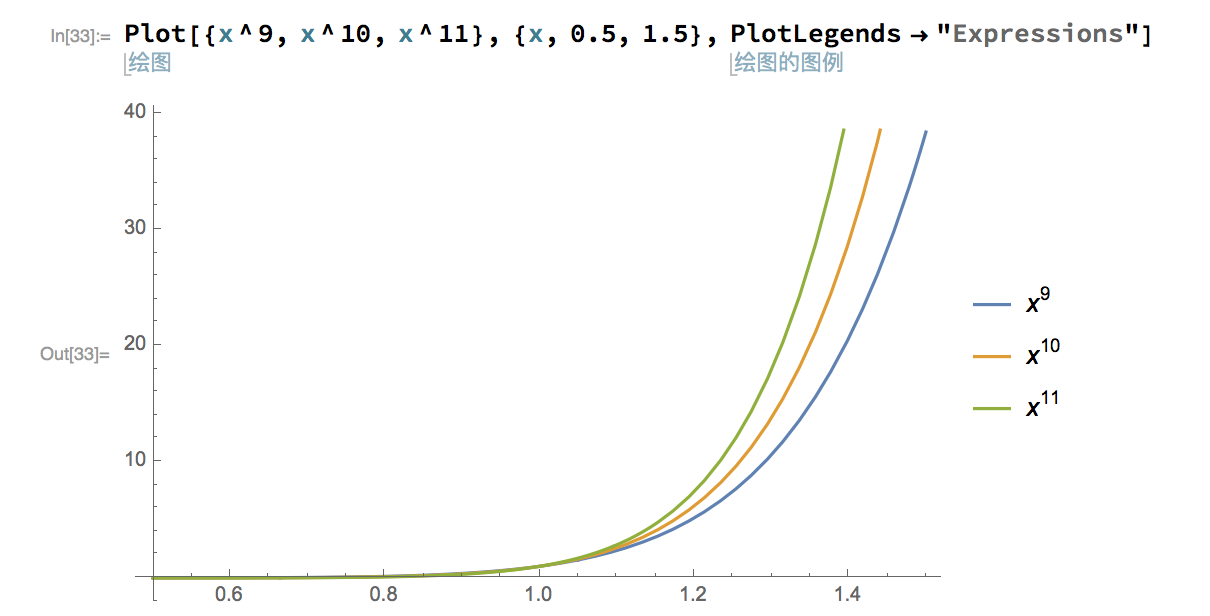
\includegraphics[width=12cm]{./Figures/20170917-monomial-mcl}
  \label{fig:pj-spectral-monomials}
%
%  \small{Source: PBOC.}
\end{figure}



单项式基的上述缺点,使得我们寻求利用正交多项式构建基方程。内积形式的正交多项式的值相对于$x$的变化往往较为平缓,并且在加入更高次多项式元素后,系统会出现足够大的变化,有助于更精确近似原系统中的方程$d(\cdot)$。

\subsection{三角序列}
\label{sec:pj-base-spectral-trigonometric}
光谱法全局基的另一选项是三角序列(trigonometric series)\index{basis!trigonometric series \dotfill 三角序列(基)},如
\begin{equation*}
  \frac{1}{\sqrt{2 \pi}},
  \frac{\cos x}{\sqrt{2 \pi}},
  \frac{\sin x}{\sqrt{2 \pi}},
  \ldots,
  \frac{\cos k x}{\sqrt{2 \pi}},
  \frac{\sin k x}{\sqrt{2 \pi}},
  \ldots
\end{equation*}

三角序列适合用于分析有周期性特征的方程,因而在自然科学和工程学中得到广泛应用。遗憾的是除了时间序列分析等领域之外,经济学研究的问题较少涉及到周期性。此外,目前将周期性方程近似为非周期性方程的方法尚未成熟。因此我们不做深入探讨。

\subsection{雅各比多项式}
\label{sec:pj-base-spectral-jacobi-poly}
雅各比多项式\index{basis!Jacobi polynomial \dotfill 雅各比多项式(基)}(第\ref{sec:poly-jacobi-polynomial}节)也适合作为光谱法全局基的选项之一。

雅各比多项式一族中,还包括盖根鲍尔多项式(Gegenbauer), 勒让德(Legendre),切比雪夫多项式(Chebyshev),他们可以相互转换。\cite[Table 1]{Boyd:2013kj}比较了几种多项式在处理不同优化指标时的性能排序,从而提供了重要参考:在绝大多数情况下,对于求解DSGE模型的工作来说,最适于采用切比雪夫多项式构建基方程。

\subsection{切比雪夫多项式}
\label{sec:pj-base-spectral-chebyshev-poly}
切比雪夫多项式\index{basis!Chebyshev polynomial \dotfill 切比雪夫多项式(基)}(第\ref{sec:poly-chebyshev-polynomial}节)作为光谱法全局基的选项之一,具有许多优点:
\begin{enumerate}
  \item 便于在各种表述形式之间互相转换,如罗德里格斯公式、三项递推关系、母方程
  、二阶导数线性方程等。
  \item 可以通过余弦换算,迅速计算系数变化后的值。
  \item 切比雪夫插值(interpolation)换算的结果,比其他几种多项式插值的结果更为稳健。
  \item 切比雪夫多项式是平滑的,并且有界(闭区间$[-1,1]$)。
  \item 切比雪夫差值的误差,可以由一系列定理得到较好的限制。
\end{enumerate}

第一类切比雪夫多项式$T_n(x)$满足关系$T_n(0)=1, T_n(1)=x, T_{n+1}(x) = 2x T_n(x) - T_{n-1}(x)$,因此我们可得到一组多项式序列$1, x, 2x^2-1, 4x^3 - 3x, 8x^4 - 8x^2 + 1, \ldots$,随着$n=0,1,2,\ldots,7$,我们绘制出了$T_n(x)$的曲线,见\ref{fig:pj-spectral-chebyshev}。不难看出,$n=0$时是条平行线,$n=1$时是$45$度斜线,$n=2$时是一条抛物线,随着$n$逐渐增加,切比雪夫多项式的曲线形状呈波浪状。
\begin{figure}[htbp]
   \caption{切比雪夫多项式$T_n(x)$}
  \centering
  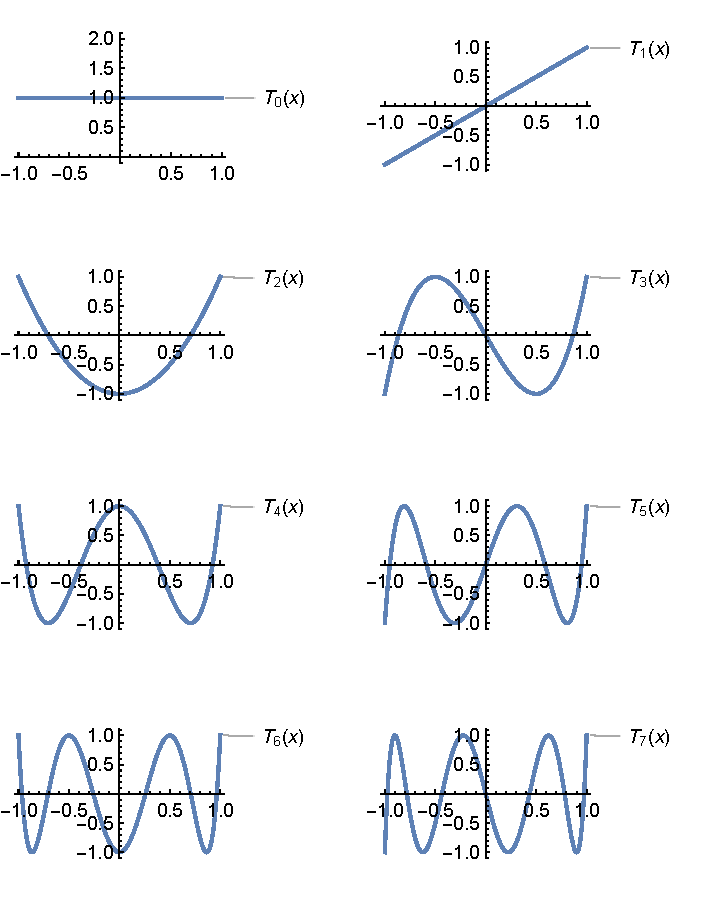
\includegraphics[width=15cm]{./Figures/20170917-chebyshev-poly}
  \label{fig:pj-spectral-chebyshev}
%
%  \small{Source: PBOC.}
\end{figure}

图\ref{fig:pj-spectral-chebyshev}在Mathematica中输入如下命令生成:
\begin{verbatim}
  t0 = Plot[{ChebyshevT[0, x]}, {x, -1, 1}, PlotLabels -> "Expressions"];
  t1 = Plot[{ChebyshevT[1, x]}, {x, -1, 1}, PlotLabels -> "Expressions"];
  t2 = Plot[{ChebyshevT[2, x]}, {x, -1, 1}, PlotLabels -> "Expressions"];
  t3 = Plot[{ChebyshevT[3, x]}, {x, -1, 1}, PlotLabels -> "Expressions"];
  t4 = Plot[{ChebyshevT[4, x]}, {x, -1, 1}, PlotLabels -> "Expressions"];
  t5 = Plot[{ChebyshevT[5, x]}, {x, -1, 1}, PlotLabels -> "Expressions"];
  t6 = Plot[{ChebyshevT[6, x]}, {x, -1, 1}, PlotLabels -> "Expressions"];
  t7 = Plot[{ChebyshevT[7, x]}, {x, -1, 1}, PlotLabels -> "Expressions"];
  GraphicsGrid[{{t0, t1}, {t2, t3}, {t4, t5}, {t6, t7}}]
\end{verbatim}


第$n$次切比雪夫多项式$T_n(x)$有$n$个根,对应
\begin{equation}
  \label{eq:pj-spectral-cheby-roots-n}
  x_k = \cos \left( \frac{2k - 1}{2n} \pi \right), \quad k = 1, 2, \ldots, n, -1 \le x_k \le 1,
\end{equation}
如图\ref{fig:pj-spectral-cheby-roots-n}所示,所有根都在闭区间$[-1,1]$之间。
\begin{figure}[htbp]
   \caption[切比雪夫多项式的根]{切比雪夫多项式$T_n(x)$的根$x_k, n=100, k=1,2,\ldots,n$}
  \centering
  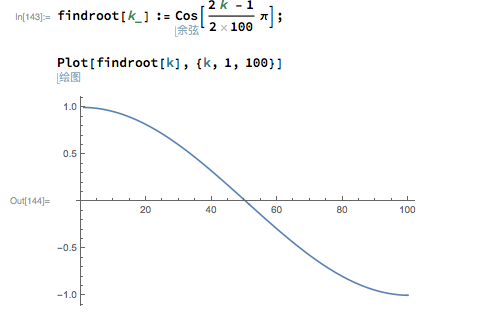
\includegraphics[width=8cm]{./Figures/20170917-cheb-roots-n-range}
  \label{fig:pj-spectral-cheby-roots-n}

  \small{说明:计算等式依据\eqref{eq:pj-spectral-cheby-roots-n}。}
\end{figure}

大多数DSGE模型的状态变量域$x \in [a,b]$,$a,b \neq \pm 1$,在实际研究中我们常采用如下线性关系转换,将它转换为$[-1,1]$区间内的值,以符合切比雪夫多项式的要求:
\begin{equation}
  \label{eq:pj-state-transformation-chebysev-interval}
  2 \frac{x-a}{b-a} -1,
\end{equation}
详见第\ref{sec:pj-spectral-cheby-variable-change}节。
例如$(a=-7,b=5)$的某状态变量线性转换,如图\eqref{fig:pj-state-transformation-chebysev-interval}所示。
\begin{figure}[htbp]
   \caption[切比雪夫多项式的根]{切比雪夫多项式$T_n(x)$的根$x_k, n=100, k=1,2,\ldots,n$}
  \centering
  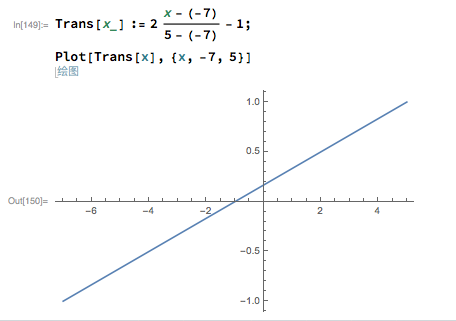
\includegraphics[width=8cm]{./Figures/20170917-linear-trans-state-chebyshev}
  \label{fig:pj-state-transformation-chebysev-interval}

  \small{说明:计算等式依据\eqref{eq:pj-state-transformation-chebysev-interval}。}
\end{figure}

使用切比雪夫多项式作为映射基,有两个定理值得关注:
\begin{enumerate}
  \item 切比雪夫插值定理(Chebyshev interpolation theorem)\index{interpolation!Chebyshev \dotfill 切比雪夫插值},见附录\ref{sec:poly-chebyshev-interpolation}:如果近似方程恰好是第$n_1$次切比雪夫多项式的根,那么随着$n_1 \rightarrow \infty$,近似误差逐渐减少到足够小的程度。根据切比雪夫插值定理,可以使用切比雪夫多项式的根作为正交配点(orthogonal collocation) \index{collocation! \dotfill 配点}\index{collocation!orthogonal \dotfill 正交配点},见\ref{sec:pj-fem}节FEM方法介绍。
  \item 切比雪夫截断定理(Chebyshev truncation theorem)\index{truncation!Chebyshev \dotfill 切比雪夫截断},见附录\ref{theorem:poly-cheby-truncation-theorem}。进而在特定情况下,切比雪夫向未知原方程做几何收敛(geometric convergence),可以表示为
  \begin{equation*}
    d(x) - d^j(x | \theta) \sim \bm{O}(\theta_j),
  \end{equation*}
  即是说,当切比雪夫近似停止于第$j$次多项式时,对应的截断误差与$j$次切比雪夫多项式系数$\theta_j$是同次的。

  根据该定理,我们可以设计一种数值检测机制:如截断误差大于某一阈值,则意味着$j$次切比雪夫近似$T_j(x)$的精度不够,需要再增加一次近似至$T_{j+1}(x)$。我们将在下文进一步讨论该问题\todo{reference}。
\end{enumerate}

\subsubsection{变量的变换}
\label{sec:pj-spectral-cheby-variable-change}

如前所述,\ref{eq:pj-state-transformation-chebysev-interval}提供了一种可将$x \in [a,b], a < -1, b > 1$转化为$[-1,1]$区间中变量的方法,以便进行切比雪夫多项式近似。在扰动法中我们也讨论了变量的变换,见\ref{sec:perturbation-change-variables}节。二者尽管技术细节有所不同,但核心思路是相同的:都是为了尽可能提高近似的精确度。本节以随机NCGT模型为例,介绍为何通过变量变化有助于提高映射法的近似精度。

原目标为寻找经济系统方程组
\begin{align*}
  &c_t = d^1(k_t,z_t), \\
  &k_{t+1} = d^2(k_t,z_t)
\end{align*}
的近似解。我们可以通过变量变换,改为寻求方程组
\begin{align*}
  &\log c_t = d^1(\log k_t, z_t),\\
  &\log k_{t+1} = d^2 (\log k_{t}, z_t)
\end{align*}
的近似解,用映射法表示为
\begin{align*}
  &\log c_t = d^{1,j}(\log k_t, z_t|\theta^1) = \sum_{i=0}^{j} \theta^1_i \psi_i (\log k_t, z_t),\\
  &\log k_{t+1} = d^{2,j} (\log k_{t}, z_t | \theta^2 ) = \sum_{i=0}^{j} \theta_i^2 \psi_i (\log k_t, z_t).
\end{align*}

\subsubsection{伯依德原则}
前文简要介绍了利用切比雪夫多项式从事经济学研究所具有的理论优势。但近些年来的经验研究,尤其是基于DSGE模型的经济学研究,越来越多地使用基于切比雪夫多项式的映射法,切比雪夫多项式作为基方程的备选方案,其巨大优势得到了越来越广泛的认可\citep{Aruoba:2006cz,Caldara:2012fr}。

\cite[p.10]{Boyd:2001wt}用一种近似于开玩笑的方式,总结了这几十年来的研究经验,将之命名为``道德准则一号'':
\begin{enumerate}
  \item 当不确定用什么基时,就用切比雪夫多项式。除非模型呈现出较强的周期性,这时可以考虑用傅里叶序列。
  \item 除非你确定其他某种基方程更好,不然就用切比雪夫多项式。
  \item 除非你非常非常确定其他某种基方程更好,不然就用切比雪夫多项式。
\end{enumerate}

\section{局部基的选取(1)}
\label{sec:pj-method-local}

第\ref{sec:pj-spectral-method-global}节所介绍的几种方案,全部都是单维度基方程,相对简单,易于我们理解用映射法求解DSGE模型的基本思路。然而现实世界中大多数经济问题都是多维度的,几乎全部DSGE模型都研究一个以上的状态变量。这就需要我们探讨多维基的选择方案。

如何选取多维基成为映射法的关键问题。然而映射法受到维数灾难(curse of dimensionality)\index{curse of dimensionality \dotfill 维数灾难}的强烈冲击\citep{Bellman:1957tx}。随着解释变量数量的增加——如中等规模DSGE模型可能要处理超过20组解释变量——应用映射法求解模型变得异常困难,这要求我们用更高的技巧去选取多维基方程。

\subsection{离散状态变量}
\label{sec:pj-multidimen-discrete-state-variables}
前文一系列分析均暗含假定,状态变量是连续的。然而在很多DSGE模型中,至少一部分变量是离散的:
\begin{itemize}
  \item 状态变量本身是离散的,如
  \begin{itemize}
    \item 财政政策,政府可能处于主权债务违约或未违约状态\citep{Bocola:2016ij},
    \item 货币政策,可能是积极的或者消极的\citep{Leeper:1991kq},
  \end{itemize}
  \item 出于计算求解的考虑,益于将连续状态变量做离散化处理,如
  \begin{itemize}
    \item 外生随机过程(技术冲击、偏好冲击等)的离散化。
  \end{itemize}
\end{itemize}

研究发现,有限马尔科夫链(finite Markov chain)\index{Markov chain!finite \dotfill 有限马尔科夫链}能够产生与连续过程相同的样本矩;经验分析表明,在大多数情况下,含有5-7个状态的马尔科夫链足够模拟一般情况下的随机过程信息,供经济学定量分析使用\citep{Tauchen:1986gi, Kopecky:2010du}。因此状态变量的离散化问题可以理解为,针对某一个连续变量,我们寻找另一个(离散的)决策方程来描述它\footnote{我们不对马尔科夫链做过多介绍(来不及把笔记敲进硬盘了)。讲义可参考帝国理工大学Emma J McCoy M3S4/M4S4 - Applied Probability的讲义第六章:Markov Chains, \url{http://101.96.10.63/wwwf.imperial.ac.uk/~ejm/M3S4/NOTES3.pdf}。教材可参考\cite{Privault:2013vc}。}。

仍然以含有随机NCGT模型为例,假定外生技术冲击$z_t$是一个一阶自回归过程$AR(1)$
\begin{equation*}
  z_t = \rho z_{t-1} + \varepsilon_t,
\end{equation*}
其中$\varepsilon_t \sim N(0,\sigma^2_z)$是一个平稳分布(stationary distribution)\index{distribution!stationary \dotfill 平稳分布}。

可以表示为含有$n$个点的马尔科夫过程$z_t \in \{ z_1, z_2, \ldots z_n \}$,对应转移矩阵$P_{z,z'}$ (transition matrix)\index{transition matrix \dotfill 转移矩阵}
\begin{equation}
  \label{pj-discrete-transition-matrix-def}
  P_{z,z'}=\begin{pmatrix}
  p_{11}& \ldots &p_{1n} \\
  p_{21}& \ldots &p_{2n} \\
  \vdots& \ddots & \vdots \\
  p_{n1} & \ldots & p_{nn}
  \end{pmatrix},
\end{equation}
其中转移概率(transition probability)\index{transition probability \dotfill 转移概率} $p_{i,j}$ 表示当前期处于位置$i$马尔科夫链下一时期转移到位置$j$的概率。

将AR(1)过程$z_t$离散化的常见算法,见附录第\ref{sec:pj-local-discretization}节。

(注意,建议阅读这个附录,以便弄明白是怎么回事,还有附带的matlab代码。)

将技术冲击离散化后,我们的研究目标就变为,寻找$2 \times n$个决策方程:
\begin{equation*}
  \begin{split}
    &c \left( k, z_m \right) = d^{c,m,j} \left( k | \theta^{m,c} \right) = \sum_{i=0}^{j} \theta_{i}^{m,c} \psi_i(k), \\
    &k \left( k, z_m \right) = d^{k,m,j} \left( k | \theta^{m,k} \right) = \sum_{i=0}^{j} \theta_{i}^{m,k} \psi_i(k),
  \end{split}
\end{equation*}
其中$m=1,2,\ldots,n$。举例来说,我们首先寻找当今天的技术水平是$z_1$时资本和消费的决策方程,进而寻找当今天的技术水平是$z_2$时资本和消费的决策方程,随后$z_3, \ldots, z_m, \ldots, z_n$。为了让数值运算不至于太过复杂,我们常将$n$控制在一个比较小的值上,比如5到7之间。

在求得两个决策方程后,代回到原系统的欧拉方程
\begin{equation}
  \label{eq:pj-local-euler-eq}
  u'(c_t) = \beta E_t \left[ u'\left( c_{t+1} \right) \left( \alpha \exp(z_{t+1}) k_{t+1}^{\alpha - 1} + 1 - \delta \right) \right]
\end{equation}
中,我们有
\begin{equation}
  \label{eq:pj-local-euler-eq-discrete}
  \begin{split}
    u'\left( d^{c,m,j} \left( k | \theta^{m,c} \right)\right) = \beta \sum_{l=0}^{n} p_{ml} &\left[
    u'\left(
    d^{c,l,j}
    \left( d^{k,m,j} \left( k | \theta^{m,k} \right) | \theta^{l,c} \right)
     \right) \right. \\
     & \left. \left(
     \alpha \exp(z_{t+1})
     \left(
     d^{k,m,j} \left( k | \theta^{m,k} \right)
    \right)^{\alpha-1}
     + 1 - \delta
     \right)
    \right]
  \end{split}
\end{equation}

\eqref{eq:pj-local-euler-eq-discrete}中有两点值得注意
\begin{enumerate}
  \item 近似算法中$2 \times n$个决策方程都是当期的,不过上式中$t+1$的决策方程,依然考虑到$t+1$期可能出现的技术水平变化。
  \item  由于我们将随机过程进行离散化近似,对应地,积分形式的RHS被简化为离散求和形式,乘以转移矩阵\eqref{pj-discrete-transition-matrix-def}中的相应元素\footnote{也有一些研究直接从积分形式入手,探讨一系列求积法,可参考\cite{Judd:1998uy,Judd:2011iw}。}。
\end{enumerate}

因此,在存在多维度问题的DSGE模型中,常常可以对其中至少一部分状态变量如技术冲击做离散化处理,其优点在于简单直观,操作过程透明,并且不是特别耗费计算资源。以及在一定意义上,求解DSGE模型往往依赖于混合策略:对一部分连续状态变量做离散化处理,对剩余的连续变量采用其他近似策略,如张量、完全多项式等,见下文。


\subsection{张量与完全多项式}
\label{sec:pj-multidimen-tensor}
张量(tensors)\index{tensor \dotfill 张量}将一组单维的基方程,用克罗内克乘积\footnote{见式\eqref{eq:poly-kronecker}。}的组合在一起,构成多维基方程。例如一个经济系统中有两个状态变量,实物资本$k_t$和人力资本$h_t$,每个状态变量分别对应3个切比雪夫多项式:
\begin{equation*}
  \begin{split}
    &\psi_{0}^k(k_t),\psi_{1}^k(k_t),\psi_{2}^k(k_t),\\
    &\psi_{0}^h(h_t),\psi_{1}^h(h_t),\psi_{2}^h(h_t).
  \end{split}
\end{equation*}

则我们可以构建一个张量作为基方程
\begin{equation*}
  \begin{split}
    &\psi_{0}^{k}(k_t) \psi_{0}^{h}(h_t),
    \psi_{0}^{k}(k_t) \psi_{1}^{h}(h_t),
    \psi_{0}^{k}(k_t) \psi_{2}^{h}(h_t), \\
    &\psi_{1}^{k}(k_t) \psi_{0}^{h}(h_t),
    \psi_{1}^{k}(k_t) \psi_{1}^{h}(h_t),
    \psi_{1}^{k}(k_t) \psi_{2}^{h}(h_t), \\
    &\psi_{2}^{k}(k_t) \psi_{0}^{h}(h_t),
    \psi_{2}^{k}(k_t) \psi_{1}^{h}(h_t),
    \psi_{2}^{k}(k_t) \psi_{2}^{h}(h_t).
  \end{split}
\end{equation*}

进而,对于一个有$n$个状态变量的方程系统$d:[-1,1]^n \rightarrow \mathbb{R}$,我们试图用$j$次切比雪夫多项式予以近似,则可用如下张量形式表现
\begin{equation*}
  d^j(\cdot | \theta) = \sum_{i_1 = 0}^{j} \sum_{i_2 = 0}^{j} \ldots \sum_{i_n = 0}^{j} \theta_{i_1, i_2, \ldots, i_n} \, \psi_{i_1}^{1}(\cdot) * \ldots  \psi_{i_n}^{n}(\cdot),
\end{equation*}
其中$\psi_{i_\kappa}^{\kappa}$是第$\kappa$个状态变量的$i_{\kappa}$次切比雪夫多项式,$\kappa = 1,2,\ldots,n$;系数向量$\theta$为$\left\{ \theta_{i_1}, \theta_{i_2}, \ldots, \theta_{i_n} \right\}$。

采用张量基方程有如下优点,
\begin{enumerate}
  \item 易于构建
  \item 传递性:如果组成张量的单维基方程是正交的,那么由单维基乘积组成的张量基方程也是正交的。
\end{enumerate}
最显著的不足在于维数灾难\index{curse of dimensionality \dotfill 维数灾难}:待求解系数$\theta_{i_1, \ldots i_{n}}$的个数随着$j$和$n$的增加而指数增加,呈$(j+1)^n$形。上例中$j=2,n=2$对应需要近似计算$9$个系数;图\ref{fig:pj-local-tensor-simu}。
\begin{equation*}
(j+1)^n =
\begin{cases}
    256 & (j,n)=(3,4)\\
    3125 & (j,n)=(4,5)\\
    46656 & (j,n)=(5,6)\\
    \ldots
\end{cases}
\end{equation*}
\begin{figure}[htbp]
   \caption[张量模拟]{张量代求解系数的数量$(j=1)^n$}
  \centering
  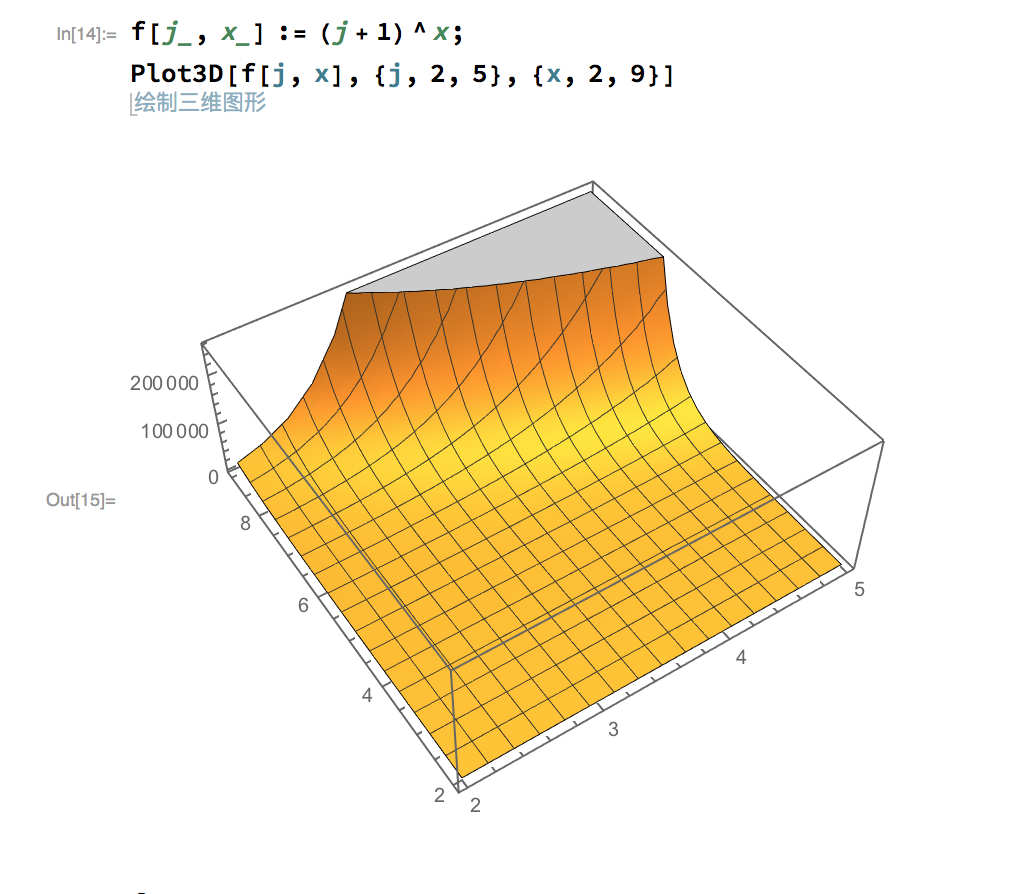
\includegraphics[width=8cm]{./Figures/20170920-tensor-coefficient}
  \label{fig:pj-local-tensor-simu}
%
%  \small{Source: PBOC.}
\end{figure}

在实际研究中,当模型里有$n>3$个连续状态变量和1个哪怕是中等规模的$j$时,张量基的方法便不易展开了。一个方法是去掉张量集合中的部分元素,以减轻计算负担。\cite{Gaspar:1997we}建议使用完全多项式(complete polynomials)\index{polynomial!complete \dotfill 完全多项式}:
\begin{equation}
\begin{split}
    \mathcal{P}^n_{\kappa} \equiv & \left\{ \psi_{i_1}^1 * \ldots * \psi_{i_n}^n \right\}, \left| \bm{i} \right| \le \kappa ,\\
    & \left| \bm{i} \right| = \sum_{l=1}^n i_l, \quad 0 \le i_1,\ldots,i_n,
\end{split}
\end{equation}
即是说,首先预设一个正整数值$\kappa$,进而在张量中,只选取各个基方程的级数之和小于$\kappa$所对应的那部分元素。这是基于下述认识:对于描述原方程系统$d$的目标而言,绝大多数信息都已经在完全多项式$\mathcal{P}^n_{\kappa}$中体现出来了;余下的部分$ \psi_{i_1}^1 * \ldots * \psi_{i_n}^n, \left| \bm{i} \right| > \kappa $ 只能给基方程产生有限的信息,却是以大量额外计算时间为代价的。

举例来说,对于$j=4,n=3$的张量系统,有$(4+1)^3=125$个元素。我们设$\kappa = 6$,提取$\left| \bm{i} \right| \le 6$的部分构建完全多项式$\mathcal{P}_6^3$,则只需要近似计算其中的87个系数了。

不幸的是,这仍然太多。在下文\todo{reference}中我们进一步介绍斯莫尔亚克稀疏网格算法。

\section{局部基的选取(2):有限元法}
\label{sec:pj-fem}

作为局部基方法的一种,有限元法(finite elements method, FEM)\index{finite elements method \dotfill 有限元法} 由\cite{McGrattan:1996gu}最先在经济学研究中倡导并予以实践\footnote{有限元法的数理知识,可见教材\cite{Hughes:2000ve, Brenner:2008hf}。可参考Joseph E. Flaherty的讲义 CSCI, MATH 6860: Finite Element Analysis \url{http://www.cs.rpi.edu/~flaherje/FEM/index4.html}。}。

有限元法常应用在一些关键任务的工业领域,如航空航天,核电厂施工等,这是由它的突出优势所决定的:可以很方便描述某些局部域内的行为,以及达到相当高的精确度。相应地,有限元法的主要不足在于难以编程,计算求解速度慢。

利用有限元法展开分析,常见的步骤如下。第一步是确定状态变量的值域$\Omega$。值域的选取方面,一些规则是天然的(如$k_t > 0$),另一些则不是($k_t < \bar{k}$),后者我们需要额外注意:如,可以将$\bar{k}$设的足够高,以至于在模型仿真过程中所有$k_t$都在上限$\bar{k}$的下方。随着仿真过程的实际展开,$\bar{k}$的值也可能做微调。

第二步是将$\Omega$分成若彼此不重叠的有限个元。各个元相接的部分称为结点(nodes)\index{node \dotfill 结点}。分元的原则总体上来讲灵活性很高,可以
\begin{itemize}
  \item 均等划分,直观简便
  \item 根据变量处于某种状态的频率,划分为一系列小块(频率高)和大块(频率低)。对``频率''的设定又分为两种情况
  \begin{itemize}
    \item 来自理论模型系统的特征
    \item 利用迭代法,对所划分元的事后验证\todo{见下文,补reference。}
  \end{itemize}
  \item 在$\Omega$中,将$d(\cdot)$变化幅度较大的部分划分为小元,相对变化幅度不大的部分划分为大元,从而在每一个元内部,原本是非线性的$d(\cdot)$接近线性。
\end{itemize}

在工程实践中,得益于灵活的分元,有限元法可以更好处理kinks或者一些特殊限制条件\footnote{kinks通常是指,分元后,两个元的衔接处 (interface) 出现偏移(弱kinks)甚至断裂(强kinks)的情况,见图\ref{fig:pj-kinks}。}。面对这些kinks、或限制条件,一方面光谱法的操作难度较大,另一方面由于不满足可微、连续等条件,扰动法很难展开。
\begin{figure}[htbp]
   \caption[kinks]{弱kinks和强kinks的示例图}
  \centering
  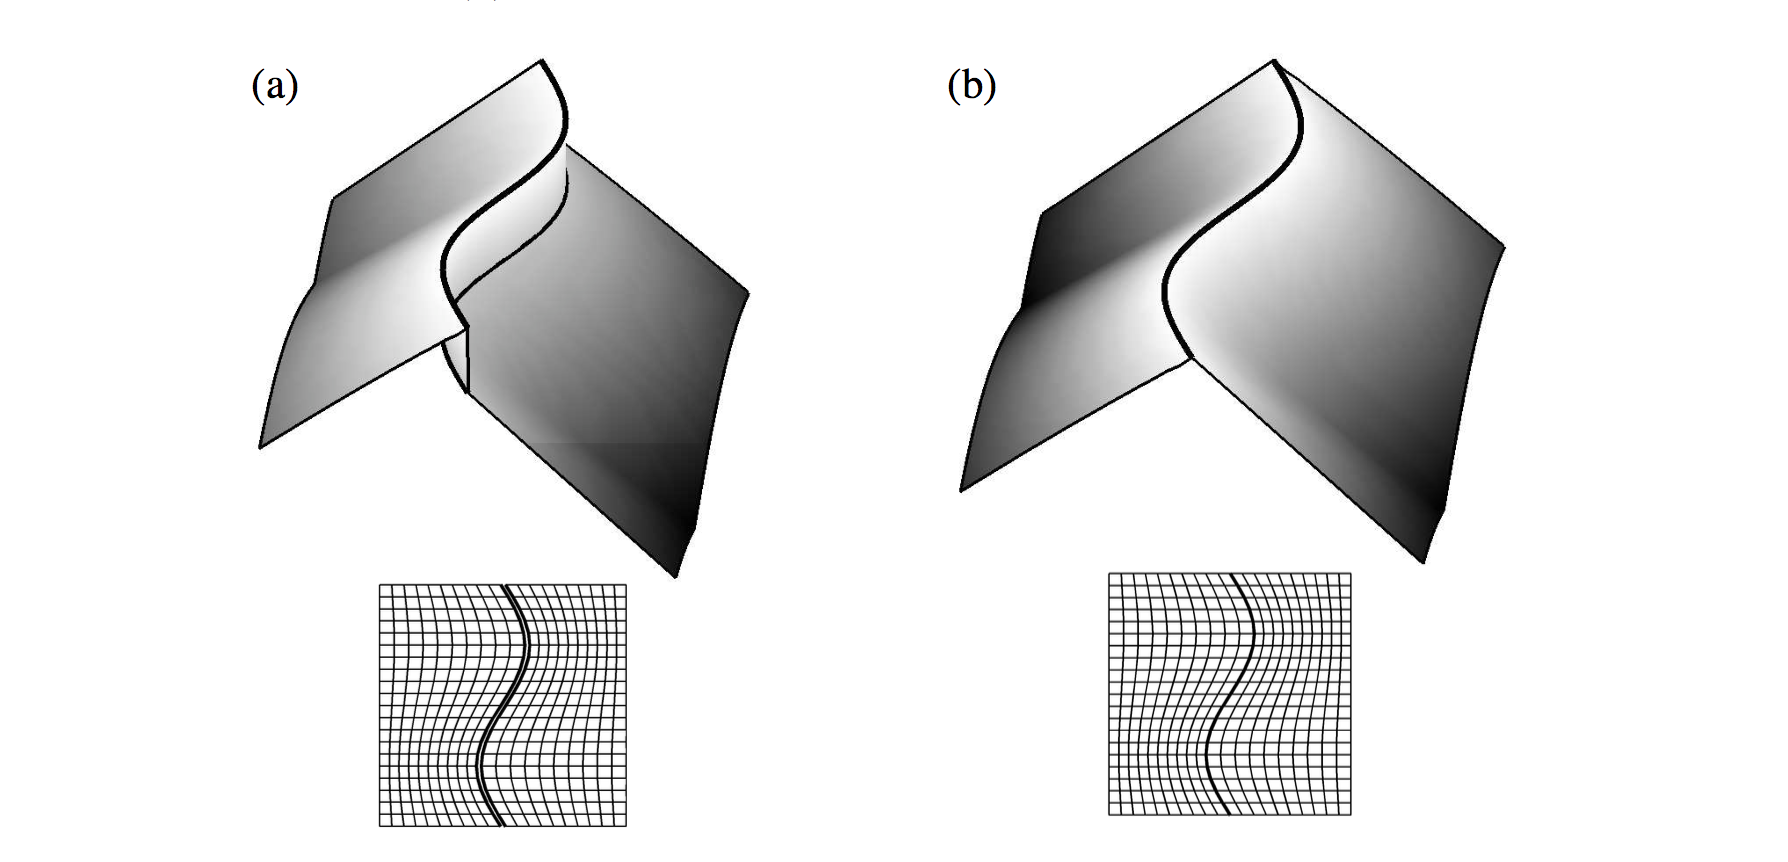
\includegraphics[width=10cm]{./Figures/20170921-kinks-fem}
  \label{fig:pj-kinks}

  \small{图片来源:\cite[Figure 2]{Fries:2010hj}。}
\end{figure}

将$\Omega$域分为有限个元素的的最优方法(网格生成 grid generation \index{grid \dotfill 网格}),已有大量工程学、数学方面的讨论,如\cite{Thompson:1985ug}。在内生NCGT模型中应用网格优化法生成有限个不均等的元以优化计算时间,可见\cite{FernandezVillaverde:2004fg}。

第三步,在每一个元中选择对应的基,用于构建政策方程。如果前述步骤中元素的划分已经有效,则这一步中的基只设定线性形式即可。例如,$\Omega$中诸元的节点表示为$\{k_0, k_1, \ldots k_j\}$,则可以定义基方程$\psi_{i}(k)$为三角函数形式,$i = 1,2,\ldots,j-1$:
\begin{subequations}
\label{eq:pj-fem-base-tent}
\begin{align}
  \label{eq:pj-fem-base-tent-a}
  &\psi_0(k) =
  \begin{cases}
  \frac{k_0 - k}{k_1-k} , \text{如果} k \in [k_0,k_1], \\
  0,
  \end{cases} \\
  \label{eq:pj-fem-base-tent-b}
  &\psi_i(k) =
  \begin{cases}
    \frac{k - k_{i-1}}{k_i - k_{i-1}}, \text{如果} k \in [k_{i-1},k_{i}],\\
    \frac{k_{i+1} - k}{k_{i+1} - k_i}, \text{如果} k \in [k_{i},k_{i+1}], \\
    0,
  \end{cases}\\
  \label{eq:pj-fem-base-tent-c}
  &\psi_j(k) =
  \begin{cases}
  \frac{k - k_{j-1}}{k_{j}-k_{j-1}}, \text{如果} k \in [k_{j-1},k_{j}],\\
  0.
  \end{cases}
\end{align}
\end{subequations}

之所以说\eqref{eq:pj-fem-base-tent}的基方程是三角形式,举例说明,见图\ref{fig:pj-fem-tent}。
\begin{figure}[htbp]
   \caption{三角方程形式}
  \centering
  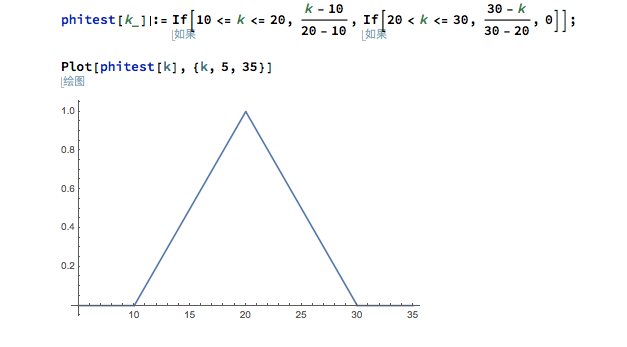
\includegraphics[width=10cm]{./Figures/20170921-tent-function}
  \label{fig:pj-fem-tent}
%
%  \small{Source: PBOC.}
\end{figure}

第四步,与其他映射法类似,生成决策方程系统作为原方程系统的近似,在有限元分析中我们常称之为分段线性近似(piecewise linear approximation)。
\begin{equation*}
  d^{n,j}\left( \cdot | \theta^n \right) = \sum_{i=0}^{j} \theta^n_i \psi_{i} \left( \cdot \right),
\end{equation*}
将近似系统代回$\mathcal{H}$。其中,$\theta$和$\psi$由切比雪夫多项式的相关算法求得:以本例中的有限元节点$k_i$和$k_{i+1}$为例,分别对应基方程
\begin{equation*}
  \begin{split}
    \psi_{i}(k) = \frac{k_{i+1} - k}{k_{i+1} - k_{i}}, \\
    \psi_{i+1}(k) = \frac{k - k_{i}}{k_{i+1} - k_i},
  \end{split}
\end{equation*}
那么由节点$k_i$和$k_{i+1}$划出的元中,值$d^{n,j}\left( \cdot | \theta^n \right)$由一个近似方程$\hat{d}$表示
\begin{equation*}
\begin{split}
    \hat{d} \left( k | k_{i}, k_{i+1}, \theta^n_i, \theta^n_{i+1} \right) &= \theta_i^n \psi_i(k) + \theta_{i+1}^n \psi_{i+1}(k) =\theta_i^n \frac{k_{i+1} - k}{k_{i+1} - k_{i}} + \theta_{i+1}^n \frac{k - k_{i}}{k_{i+1} - k_i} \\
    &= \frac{
    \left( \theta_{i+1}^n - \theta_{i}^n \right) k + \theta_{i}^n k_{i+1} - \theta_{i+1}^n k_{i}
    }{k_{i+1} - k_i},
\end{split}
\end{equation*}
不难看出,近似方程$\hat{d}$是线性的,斜率的符号由$\theta_{i+1}^n - \theta_{i}^n$来决定。

另一方面采用类似的方法,以有限元结点$k_{i-1}$和$k_{i}$划出的元中,我们可以得到另一个线性近似方程$\hat{d}$
\begin{equation*}
  \hat{d} \left( k | k_{i-1}, k_{i}, \theta^n_{i-1}, \theta^n_{i} \right)=
  \frac{
  \left( \theta_{i}^n - \theta_{i-1}^n \right) k + \theta_{i-1}^n k_{i} - \theta_{i}^n k_{i-1}
  }{k_{i} - k_{i-1}}。
\end{equation*}

两个元在$k_i$处相交,此时我们有
\begin{equation*}
  \begin{cases}
    \hat{d} \left( k_{i} | k_{i}, k_{i+1}, \theta^n_i, \theta^n_{i+1} \right)  = \theta^n_i, \\
    \hat{d} \left( k_i | k_{i-1}, k_{i}, \theta^n_{i-1}, \theta^n_{i} \right)= \theta^n_i,
  \end{cases}
\end{equation*}
即两个方程等于一个相同的值$\theta^n_i$,这确保了作为各个$\hat{d}$的加总的$d$方程是连续的。

上述介绍也说明为何有限元法提供的分段线性近似\index{piecewise linear approximation \dotfill 分段线性近似}是个较为理想的近似策略。假定我们设对应的度量方程$\rho(\cdot)$的形式为\footnote{度量方程的选取方案有数种,这里只举其中之一;更多讨论见下节。}\todo{reference},使得在划分元所依据的每个节点$k_i$上,都有残差方程$R(\cdot) = 0$。对于三角函数形式的分段基方程$\psi_i(\cdot)$而言,这意味着当状态变量处在$k_i$节点上时,对系数$\theta^n_i$的取值应当使得近似方程系统与原方程系统相等:
\begin{equation*}
  \hat{d}^{n,j}(\cdot | \theta^n) = d^n(\cdot).
\end{equation*}

需要指出的是,有限元分析中的分段线性近似法也表明,系数$\theta^n_i$的选取,与状态变量处于节点$k_i$之外其他位置时$d^n(\cdot)$的值无关。从这个意义上来讲,利用有限元法求解大型非线性方程系统所得到的近似系统,都是稀疏的(sparse)。这成为一个可为现代非线性求解方法所利用的特征。

第五步,(如有需要)对结果的改进。如果第一轮有限元分析近似解的精度不达标,我们可以根据需要对近似解做反复改进,进行第二轮、第三轮甚至更多有限元分析,在计算时间和内存允许的范围内,尽可能提高近似解的精度。事实上这是有限元法研究的又一突出优势。在现有研究文献中,改进常常分为三大类型。
\begin{enumerate}
  \item h——改进(h-refinement)\index{h-refinement finite elements\dotfill h——改进(有限元分析)},在全部域$\Omega$内,将第一轮所分元(如$A,B,C, \ldots$)再均等分为更小的元(如$A1,A2,A3, \ldots$),对这些细分元再反复迭代使用有限元法,改善近似解,直至精度达标。
  \item r——改进(r-refinement)\index{r-refinement finite elements \dotfill r——改进(有限元分析)},第二、第三甚至更多轮有限元分解的重点针对存在着明显非线性特征的局部。
  \item p——改进(p-refinement)\index{p-refinement finite elements \dotfill p——改进(有限元分析)},不对现有元再作细分,而是在元内部通过加入更多个基方程(如更多的切比雪夫多项式)来提高近似的阶数(order);如果元内现有阶数已足够高,则应用有限元法和光谱法组合的混合策略,常称为光谱元法(spectral elements)\index{spectral elements \dotfill 光谱元}。在自然科学和工程学领域,光谱元法已得到了广泛应用\citep{Solin:2003up}。
\end{enumerate}

有时,h——和p——改进被混合在一起使用,称hp——有限元法(hp-adaptive finite elements)\index{hp-adaptive finite elements \dotfill hp——有限元法},可以使近似解以指数速度向真实解收敛\citep{Ciarlet:2002tm}。尽管它的编程难度更高,计算时间更长,但hp——有限元法可能是目前已知最强大的DSGE求解工具了,有助于求解甚至是最复杂的DSGE模型。关于这种方法的详细介绍,可参考\cite{Babuska:1994jz,Demkowicz:2006ww,Demkowicz:2007ur}。

\section{目标方程的选取}
\label{eq:pj-metric}
如前所述,映射法研究中也需要选取度量方程$\rho$作为目标方程。在未对$\mathcal{H}$作过多限定的前提下,可视$R(\cdot | \theta)$为最简单的单维情况\footnote{随着$\mathcal{H}$的限定条件变多,$R(\cdot \theta) = \mathcal{H} \left( d^j \left(\cdot \theta \right) \right)$可能变成多维度的,但在这里我们暂不做讨论。}。此时对$\rho \left( R \left( \cdot| \theta \right), \bm{0} \right)$的选取目标可设定为,使用加权残差法,选取合适的$\theta$向量,使得加权残差之的积分最接近于零,对应某个权重方程$\phi_i : \Omega \mapsto \mathbb{R}$:
\begin{equation*}
  \rho \left( R \left( \cdot| \theta \right), \bm{0} \right) = \begin{cases}
  0 & \text{如果 } \quad \int_{\Omega} \phi_i(\bm{x}) R \left( \cdot | \theta \right) d \bm{x}, \quad i = 1,2,\ldots,j+1,\\
  1,
  \end{cases}
\end{equation*}
这样问题变为在给定$j+1$个权重方程$\phi_{i}$的前提下,选择$\theta$的值来求解积分系统
\begin{equation}
  \label{pj-metric-int-des}
  \int_{\Omega} \phi_i(\bm{x}) R(\cdot | \theta) d \bm{x}, \quad  i=0,1,\ldots,j+1,
\end{equation}
对此我们有一系列常用解法可供选择,如规模较小的系统可用牛顿算法(Newton algorithm)\index{Newton algorithm \dotfill 牛顿算法},规模较大的系统可用莱文贝格——马夸特方法(Levenberg-Marquardt algorithm)\index{Levenberg-Marquardt algorithm \dotfill 莱文贝格——马夸特方法},等。然而需要指出的是,系统\eqref{pj-metric-int-des}可能无实解或者有多个解。关于如何将映射法应用到经济学经验研究中的理论依据,到目前为止我们所知不多——应用数学研究中大量关于映射法的文献,涉及解的存在性、收敛特性等问题的研究,主要针对自然科学和工程学领域,它们并不完全适用于经济学。事实上,对诸如\eqref{pj-metric-int-des}的经济系统而言,需要确保解满足DSGE模型的横截条件(transversality condition),从而使得状态变量处于稳定域内——在实际求解过程中,这边需要我们选择合适的初始猜测系数$\theta_0$,或是在求解过程中加入边界条件。

与基方程$\psi_i$类似,关于权重方程$\phi_i$也存在一系列选择方案。下面我们介绍一下经济学研究中常见的权重方程的设定方法。

\subsection{最小方差}
\label{sec:pj-weight-least-squares}
将研究目标理解为如下变分法问题(variational problem)
\begin{equation*}
  \min_{\theta} \int_{\Omega} R^2 \left( \cdot | \theta \right) d \bm{x},
\end{equation*}
一阶条件为
\begin{equation*}
  \int_{\Omega} \frac{\partial R(\bm{x} | \theta)}{ \partial \theta_{i-1}} R(\cdot | \theta) d \bm{x}, i=1,2,\ldots,j+1.
\end{equation*}
则权重方程的选取方案之一是将其定义为
\begin{equation}
  \phi_{i}(\bm{x}) = \frac{\partial R(\bm{x} | \theta)}{ \partial \theta_{i-1}}.
\end{equation}

映射法研究中,利用变分法问题设定权重方程,其思路与计量经济学中的回归问题相近似(见第\ref{sec:pj-connection-ols-econometrics}节)。

优缺点:
\begin{enumerate}
  \item 优点:直观,易于理解。
  \item 缺点:
  \begin{enumerate}
    \item 最小方差及几种变体都要求计算$\frac{R(\bm{x}|\theta)}{\theta_{i-1}}$,导致计算成本高。
    \item 最小方差问题过于复杂,条件苛刻,难于数值求解。
  \end{enumerate}
\end{enumerate}

\subsection{子域}
\label{sec:pj-weight-subdomain}
将状态变量的域$\Omega$通过一系列灵活的划分原则,分为$j+1$个子域(subdomain) $\Omega_i, \, i=1,2,\ldots,j+1$,则研究目标可以理解为如下$j+1$个求积问题
\begin{equation*}
  \int_{\Omega_i} R(\cdot | \theta) d \bm{x} = 0, \quad i=1,2,\ldots,j+_1.
\end{equation*}
则子域法将权重设为如下$j+1$个分段方程
\begin{equation*}
  \phi_i(\bm{x}) = \begin{cases}
  1 & \text{如果}\, \bm{x} \in \Omega_i,\\
  0.
  \end{cases}
\end{equation*}

优缺点基本同于第\ref{sec:pj-weight-least-squares}节的最小方差法。

\subsection{配点}
\label{sec:pj-weight-collocation}
\subsubsection{配点法}
\label{sec:pj-weight-collocation-method}
配点法(collocation method)\index{collocation! \dotfill 配点},又称伪光谱法(pseudospectral method)\index{pseudospectral \dotfill 伪光谱}或选点法(selected points method)\index{selected points \dotfill 选点},是指在状态变量域$\Omega$中选取$j+1$个配点$\bm{x}_i$,将权重方程定义为
\begin{equation*}
  \psi_i(\bm{x}) = \delta(\bm{x} - \bm{x}_i), i=1,2,\ldots,j+1,
\end{equation*}
其中$\delta$是狄拉克方程(dirac delta function, 第\ref{sec:fourier-non-pulse-functions}节)\index{dirac delta function \dotfill 狄拉克方程},满足
\begin{equation*}
  \begin{split}
    &\delta(\bm{y}_i) = \begin{cases}
    +\infty, &\text{如果 }\, \bm{y}_i \equiv \bm{x} - \bm{x}_i =0,\\
     0, &\text{如果 }\, \bm{y}_i \neq 0,
    \end{cases} \\
    &\int_{-\infty}^{+\infty} \delta(\bm{y}_i) d \bm{y}_i
 = 1.
  \end{split}
\end{equation*}

配点法假定当状态变量恰好处于选点时$\bm{x} = \bm{x}_i$,权重的值为$0$,残差方程因此也为$0$。此时不必做复杂的求积计算,只需求解$j+1$个方程系统
\begin{equation*}
  R\left( \bm{x}_i | \theta \right) =0, \quad j=1,2,\ldots,j+1.
\end{equation*}

当原方程系统$\mathcal{H}$表现出较明显的非线性特征时,配点近似方法具有较大优势。

\subsubsection{配点的选取:正交配点法}
\label{sec:pj-weight-collocation-orthogonal}

$j+1$个配点的选取方法有很多,一个常用方法称正交配点法(orthogonal collocation)\index{collocation!orthogonal \dotfill 正交配点},是指在值域$\Omega$中对于向量$\bm{x}$对应的每一组状态变量,都用$j+1$次切比雪夫多项式的根(有$j+1$个)予以表示。根据切比雪夫插值定理(定理\ref{sec:poly-chebyshev-interpolation}),利用正交配点法生成的近似方程系统,会收敛至、甚至有时是均匀收敛(uniform convergence)\index{uniform convergence \dotfill 均匀收敛}至未知方程$d$。

\subsection{伽辽金法}
\label{sec:pj-weight-galerkin}
第四种权重方程$\phi_{i}(x)$的选取方法为,设它等于近似计算过程中求得的基方程$\psi_{i-1}(x)$,满足
\begin{equation*}
  \phi_{i} = \psi_{i-1}(x),
\end{equation*}
又称伽辽金近似法(Galerkin method,第\ref{sec:pj-galerkin-approximation}节\index{Galerkin method \dotfill 伽辽金近似法})。

对应地,残差$R \left( \cdot | \theta \right)$的加权积分为$0$
\begin{equation*}
  \int_{\Omega} \psi_{i}(x) R \left( \cdot | \theta \right) \, \mathrm{d} x =0, \quad i = 1, \ldots, j+1,
\end{equation*}
即是说残差项正交于每一个对应的基方程。

伽辽金法的编程代码难写,但优点在于近似结果高度精确且稳健。如果基方程$\psi_{i}(x), \, i = 1, \ldots, j+1$在$J$上完备\footnote{完备(completeness)的定义,见第\pageref{def:completeness-space}页脚注。},那么随着$j \rightarrow \infty$,伽辽金近似会逐渐点收敛(pointwise)至真实解
\begin{equation*}
  \lim_{j \rightarrow \infty} d^{j} \left( \cdot | \theta \right) = d \left( \cdot \right),
\end{equation*}
相关证明可参考Theorem \ref{theorem:pj-galerkin-approximation-convergence},
Theorem \ref{theorem:pj-galerkin-approximation-limit-convergence}。

实际研究结果表明,$j$阶伽辽金近似的精确度,可以达到$j+1$或者$j+2$阶配点近似(伪光谱法)的程度。

\subsection{两个近似技巧}
\label{sec:pj-approximation-tips}
考虑这样一个经典的非线性方程系统
\begin{equation}
  \label{eq:pj-nonlin-sys}
  \int_{\Omega} \phi_{i}(x) R\left( \cdot | \theta \right) \, \mathrm{d} x, \quad i = 1,\ldots,j+1,
\end{equation}
当系数向量$\theta$中的元素较多时,和/或我们很难得到适当的初始猜测值$\theta_{0}$时,近似求解的计算会变得很困难。实际近似过程中,我们常用以下两个技巧来提高计算速度与近似解的稳健性。

\subsubsection{系统变形}
\label{sec:pj-approximation-tips-transformation}
求解系统\eqref{eq:pj-nonlin-sys}最大的瓶颈在于系统的非线性,并且求解难度随着非线性的程度而指数上升。因此在进行数值近似之前,常可以对系统做变形来降低非线性的程度。例如跨期消费的欧拉方程
\begin{equation*}
  \frac{1}{C_{t}} = \beta E_{t} \frac{1}{C_{t+1}} R_{t+1},
\end{equation*}
其中$R_{t+1}$表示资本的总回报率。\cite{Judd:1992gs}建议系统变形如下
\begin{equation*}
  \beta C_{t} = \left( E_{t} \frac{1}{C_{t+1}} R_{t+1} \right)^{-1},
\end{equation*}
这样LHS是线性形式,RHS比原式更接近线性形式了。对于某个状态变量$x_{t}$而言,在原来的系统中,残差$R\left( \cdot | \theta \right)$的计算方式如下
\begin{equation*}
  R\left( \cdot | \theta \right) = \frac{1}{
  C_{t} \left( x_{t} | \theta \right)
  }
  - \beta E_{t}
  \left[
  \frac{1}{
  C_{t+1} \left( x_{t} | \theta \right)
  } R_{t+1} \left( x_{t} | \theta \right)
  \right],
\end{equation*}

若是采用系统变形的思路,变形后的残差$\tilde{R} \left( \cdot | \theta \right)$计算式为
\begin{equation*}
  \tilde{R} \left( \cdot | \theta \right)
  = \beta C_{t} \left( x_{t} | \theta \right)
  - \left[
  E_{t} \frac{1}{
  C_{t+1} \left( x_{t} | \theta \right)
  } R_{t+1} \left( x_{t} | \theta \right)
  \right]^{-1}.
\end{equation*}

\subsubsection{系统规模缩减}
\label{sec:pj-approximation-tips-reduction}
如前所述,我们说\eqref{eq:pj-nonlin-sys}的规模较大时,往往是指系数$\theta$的数量较多。在近似求解过程中,常常可以分步骤进行:首先在大系统中提取一组核心变量构成小系统,近似求解小系统,将近似解输入大系统中求得最终的完整解,这个思路可称为分步求解法。当系统中含有正交基方程(如切比雪夫多项式)时,分步求解法显得非常可靠:不再直接用$j+1$个基方程来直接求解大系统,而是首先提取出$j^{'}+1 << j+1$个基方程做近似求解小系统,将其作为猜测接代入大系统中,展开下一个阶段的近似。

举例来说,我们想要求一个$m$维系统中,含有10个切比雪夫多项式的,$10 \times m$个方程的系统。首先我们做3个切比雪夫多项式,$3 \times m$个方程的小系统求解,将近似得到的系数作为大方程系统的初始猜测值的一部分,$\theta_{0} = \left[ \theta^{3}, 0_{1 \times m}, \ldots, 0_{1 \times m}\right]$,即第一组系数$\theta^{3}$来自小系统的计算,其余更多系数的初始猜测值设为$0$。由于前3个和后7个切比雪夫多项式正交,那么引入额外的7个$0$不会导致系统解发生太大改变:将$\theta^{3}$作初始猜测值因而是非常理想的。此外,由于切比雪夫多项式具有快速收敛的特点,越是高阶的切比雪夫多项式,其对应的系数就越接近于$0$,那么将$\theta^{3}$作为初始猜测值的一部分,也是有信息含量的\footnote{上例将整个系统截为两段分步展开研究。随着实际需要,可以分为更多段,在写投影法的代码时,可将这些段写为与特定数量的多项式有关,进而在一个loop循环中迭代运行程序,使得由$j'$向$j$的近似以较高速度或者较低速度进行。}。

\section{投影法求解DSGE模型举例}
\label{sec:pj-example-solution-dsge}
举一个实际案例,介绍如何应用投影法,即切比雪夫多项式和正交配点等技术,来求解DSGE模型。

\subsection{模型设定}
\label{sec:pj-example-setup}
考虑一个经典的含有内生劳动力供应决定机制的随机内生经济增长模型。假定这是个中心化模型(centralized economy)
\footnote{
用中心化经济模型来介绍投影法的应用,主要原因是...懒...投影法一样可以用于求解去中心化的经济模型,又称竞争均衡模型。并且事实上,投影法的最突出优势恰恰在于,它更适合用于分析常常处于非帕累托最优状态的分散经济体,如见第\pageref{footnote:pj-solution-approximation-tradeoff}页的讨论。
}。典型家庭的消费和劳动力供应决策,由前向CCRA效用函数来表现
\begin{equation*}
  E_{0} \sum_{t=1}^{\infty} \beta^{t-1} \frac{
  \left[
  c_{t}^{\tau} \left( 1 - \ell_{t} \right)^{1 - \tau}
  \right]^{1 - \eta}
  }{1 - \eta},
\end{equation*}
其中\begin{itemize}
\item $0 < \beta < 1$表示时间贴现,
\item $\eta$是跨期替代弹性,反映家庭的风险厌恶程度,
\item $1/\tau$是劳动力供应的Frisch替代弹性,见第\ref{sec:Frish-elasticity}节。
\item $E_{0}$,$t=0$时刻的条件期望符。
\end{itemize}

经济体中有且只有一种最终商品,总量生产函数
\begin{equation}
  \label{eq:pj-solution-example-y}
  y_{t} = \exp \left(Z_{t} \right) k_{t}^{\alpha} \ell_{t}^{1 - \alpha},
\end{equation}
其中\begin{itemize}
\item $k_{t}$是总的实物资本存量,积累形式满足运动法则
\begin{equation*}
  k_{t+1} = \left( 1 - \delta \right) k_{t} + i_{t},
\end{equation*}
$i_{t}$表示当期的实物资本投资,
\item $\ell_{t}$是总劳动力,
\item $z_{t}$表示生产率,是一个随机$AR(1)$过程,满足
\begin{equation*}
  z_{t} = \rho z_{t-1} + \epsilon_{t}, \quad \left| \rho \right| < 1, \quad \epsilon_{t} \sim \mathcal{N} \left( 0, \sigma^{2} \right),
\end{equation*}
\end{itemize}

经济体中的总资源约束条件
\begin{equation*}
  y_{t} = c_{t} + i_{t}.
\end{equation*}

\subsection{社会规划者问题}
\label{sec:pj-example-bellmann}
社会规划者问题可表示为,在给定初始条件$\left\{k_{0}, z_{0} \right\}$的情况下,追求价值方程$V \left( k_{t}, z_{t} \right)$的最大化,即贝尔曼等式(Bellman equation)\index{Bellman equation \dotfill 贝尔曼等式}

\begin{equation}
  \label{eq:pj-example-bellmann}
  \begin{split}
    & V \left( k_{t}, z_{t} \right)
    = \max_{\left\{ c_{t}, \ell_{t} \right\}}
    \frac{
    \left[
    c_{t}^{\tau} \left( 1 - \ell_{t} \right)^{1 - \tau}
    \right]^{1 - \eta}
    }{1 - \eta}
    + \beta E_{t} V_{k_{t+1}, z_{t+1}},\\
    & \text{s.t.} \begin{cases}
    k_{t+1} = \exp \left( z_{t} \right) k_{t}^{\alpha} \ell_{t}^{1 - \alpha} + \left( 1 - \delta \right) k_{t} - c_{t}, \\
    z_{t} = \rho z_{t-1} + \epsilon_{t}.
    \end{cases}
  \end{split}
\end{equation}

实际求解过程中我们只需要考虑状态变量$k_{t}$和决策变量$\ell_{t}$;$c_{t}$则时一个关于$k_{t}$和$\ell_{t}$的变量。为了说明这一点,首先我们有
\begin{equation*}
  \begin{split}
    MPL & \coloneqq \frac{\partial y_{t}}{\partial \ell_{t}} = \left( 1 - \alpha \right) \exp \left( z_{t} \right) k_{t}^{\alpha} \ell_{t}^{- \alpha}, \\
    MUC & \coloneqq \tau c_{t}^{\tau - 1} \left( 1 - \ell_{t} \right)^{1 - \tau} \left[ \cdot \right]^{-\eta}, \\
    MUL & \coloneqq - \tau \left( 1 - \tau \right) c_{t}^{\tau} \left( 1 - \ell_{t} \right)^{- \tau} \left[ \cdot \right]^{-\eta},
  \end{split}
\end{equation*}
其中$MPL$表示劳动的边际产出,$MUC, MUL$分别表示消费和劳动的边际效用(负效用)。

进而可得
\begin{equation}
  \label{eq:pj-solution-example-c}
\begin{split}
    & MUC + MUL \frac{1}{MPL} = 0, \\
    & \hookrightarrow
    \left[ \cdot \right]^{-\eta} \tau c_{t}^{\tau - 1} \left( 1 - \ell_{t} \right)^{1 - \tau} =
    \frac{
    \left[ \cdot \right]^{-\eta} \left( 1 - \tau \right) c_{t}^{\tau} \left(1 - \ell \right)^{-\tau}
    }{
    \left(1 - \alpha \right) \exp \left( z_{t} \right) k_{t}^{\alpha} \ell_{t}^{-\alpha}
    }, \\
    & \hookrightarrow
    \frac{\tau}{1 - \tau} \left( 1 - \ell_{t} \right)
    = \frac{
    c_{t}
    }{
    \left( 1- \alpha \right) \exp \left( z_{t} \right) k_{t}^{\alpha} \ell_{t}^{-\alpha}
    }, \\
    & \hookrightarrow
    c_{t} = \frac{\tau}{1-\tau} \left(1 - \alpha \right)
    \exp \left( z_{t} \right) k_{t}^{\alpha} \ell_{t}^{-\alpha} \left( 1 - \ell_{t} \right).
\end{split}
\end{equation}

\subsection{参数校准}
\label{sec:pj-example-calibration}
求解模型需要为参数赋值。本节先用参数校准,在下文介绍DSGE的估计方法时将进一步讨论参数赋值的方法\todo{做一个reference}。

\begin{equation*}
  \left(\beta, \eta, \tau, \alpha, \delta, \rho, \sigma \right) = \left( 0.991, 5.000, 0.357, 0.300, 0.0196, 0.950, 0.007 \right).
\end{equation*}
大多数参数值的选取都与经验研究中的发现相近。唯一的例外是$\eta = 5$,接近一系列经验测算值中的最高值。$\eta$的值越高,意味着消费者的风险厌恶程度越高,消费行为越是缺乏耐心。在DSGE模型中之所以取如此高的$\eta$,是为了使模型中的行为人对市场中的波动更加敏感,经济行为具有更高的预防倾向(precautionary behaviors),进而决策法则的曲率(curvature)更高。而曲率越高,就表示方程系统的非线性程度越高,从而投影法近似的难度就越大。

除此而外,还需要对$AR(1)$的外生技术冲击过程$z_{t}$做离散化处理(discretization),见第\ref{sec:pj-local-discretization}节。设$n=5$,即$\left\{ z_{1},z_{2},z_{3},z_{4},z_{5} \right\}$。无条件标准差设为$\pm 3$。进而我们有转移矩阵$P_{z,z^{'}}$,矩阵中的元素$p_{m,n}$表示当前技术水平$z_{m}$,在下一时间段变为$z_{n}$的概率。

\subsection{分步求解}
\label{sec:pj-example-steps}
在无法直接求得系统\eqref{sec:pj-example-bellmann}解析解的情况下,近似求解的目标可以分步表示如下,所需的动态规划知识,见第\ref{sec:dp}章。

第一阶段,近似价值方程$V \left( k_{t} \right)$和劳动力供应的决策法则
$\ell \left( k_{t} \right)$,设为$\left\{
V^{j} \left( k_{t} | \theta^{V,j} \right),
\ell^{j}\left(k_{t} | \theta^{\ell,j} \right)
\right\}$,其中系数为$\left\{ \theta^{\ell,j}, \theta^{V,j} \right\}$。

设5个马尔科夫链用$j=1,2,3,4,5$表示,11个切比雪夫结点$T_{i} \left( \cdot \right)$用$i=0,1,\ldots,10$表示,定义式如\eqref{eq:poly-chebyshev-1-def}。那么价值方程和劳动力供应的决策法则可以近似表示为
\begin{align}
  \label{eq:pj-exmaple-teps-value}
  & V^{j} \left( k_{t} | \theta^{V,j} \right) = \sum_{i=0}^{10} \theta_{i}^{V,j}
  T_{i} \left( k _{t} \right), \\
  \label{eq:pj-exmaple-teps-labor}
  & \ell^{j}\left(k_{t} | \theta^{\ell,j} \right) =
  \sum_{i=0}^{10} \theta_{i}^{\ell, j} T_{i} \left( k_{t} \right),
\end{align}


第二阶段,已知$\ell^{j}\left( k_{t} | \theta^{\ell,j} \right)$的近似值\eqref{eq:pj-exmaple-teps-labor}计算而得,在此基础上可计算近似值$\left\{ y^{j} \left( k_{t} \right), c^{j} \left(k_{t} \right) , k^{j} \left( k_{t} \right) \right\}$:
\begin{itemize}
\item 由总量生产函数\eqref{eq:pj-solution-example-y}可得$y^{j} \left( k_{t} \right)$
\begin{equation}
  \label{eq:pj-solution-example-y-approx}
  y^{j} \left( k_{t} \right) = \exp \left( z_{t} \right) k_{t}^{\alpha}
  \left[
  \ell^{j} \left( k_{t} | \theta^{\ell,j} \right)
  \right]^{1 - \alpha}.
\end{equation}
\item 由\eqref{eq:pj-solution-example-c}可得$c^{j} \left( k_{t} \right)$
\begin{equation}
  \label{eq:pj-solution-example-c-approx}
  c^{j} \left( k_{t} \right) =
  \frac{\tau}{1-\tau} \left(1 - \alpha \right)
  \exp \left( z_{t} \right) k_{t}^{\alpha}
  \left[ \ell^{j} \left( k_{t} | \theta^{\ell,j} \right) \right]^{- \alpha}
  \left[ 1 - \ell^{j} \left( k_{t} | \theta^{\ell,j} \right) \right].
\end{equation}
\item 下一时段的资本存量由\eqref{eq:pj-example-bellmann}给出
\begin{equation}
  \label{eq:pj-solution-example-knext-approx}
  k^{j} \left(k_{t} \right) =
  \exp \left( z_{t} \right) K_{t}^{\alpha}
  \left[ \ell^{j} \left( k_{t} | \theta^{\ell,j} \right) \right]^{1-\alpha}
  + \left( 1 - \delta \right) k_{t} - c^{j} \left( k_{t} \right).
\end{equation}
\end{itemize}

\label{footnote:pj-solution-approximation-tradeoff}
值得指出的是,上面的求解过程中,我们设一个状态变量$k_{t}$,一个决策变量$\ell_{t}$为第一阶段投影近似的对象。而类似地,也可以将分步求解的方案设计为,第一阶段投影近似消费和资本存量的决策方程,第二阶段投影近似劳动力决策和价值方程。这两个方案是等价的。这从另一个侧面印证了投影法在求解分散化的去中心经济系统时(各个部门的子系统由竞争均衡条件彼此联系起来)时,具有高度的灵活性。在实际研究中具体采取哪种方案,可以视建模难度、计算(编程)难度和研究目标之间的权衡取舍而灵活决定。

第三阶段,求解近似系数$\left\{ \theta^{\ell,j}, \theta^{V,j} \right\}$。

为了得到系统的近似解,需要确定$\left\{ \theta^{\ell,j}, \theta^{V,j} \right\}$的值:这可以通过价值方程来计算。将贝尔曼等式\eqref{eq:pj-example-bellmann}改写为
\begin{equation}
  \label{eq:pj-example-bellmann-approx}
  V^{j} \left( k_{t} | \theta^{V,j} \right)
  = \frac{
  \left\{
  \left[ c^{j} \left(k_{t} \right) \right]^{\tau}
  \left[ 1 - \ell_{t}^{j} \left( k_{t} | \theta^{\ell,j} \right) \right]^{1 - \tau}
  \right\}^{1 - \eta}
  }{1-\eta}
  + \underbrace{
  \beta E_{t} V^{j} \left( K_{t+1} | \theta^{V,j} \right)
  }_{\eqqcolon \mathcal{A}}
  ,
\end{equation}
上式已经在最优决策下,因此省去$\max$符。根据离散化的设定,当期价值方程$V^{j}(\cdot | \cdot)$在下期变为$V^{m} (\cdot | \cdot)$的概率,由转移矩阵$P_{z,z^{'}}$给出,对应其中的概率元素$p_{jm}$。以$p_{jm}$为权重,\eqref{eq:pj-example-bellmann-approx}RHS的后半部分$\mathcal{A}$可以改写为
\begin{equation*}
  \mathcal{A} \coloneqq \beta E_{t} V^{j} \left( K_{t+1} | \theta^{V,j} \right)
  = \beta \sum_{m=1}^{5} p_{jm} V^{j} \left( k^{j}(k_{t}) | \theta^{V,j} \right),
\end{equation*}
这样我们将所有对于下一时段的期望值$E_{t} \left[ \cdot \right]$写为当期项的加权和,对应权重概率$p_{jm}$。依次引入\eqref{eq:pj-exmaple-teps-value},
\eqref{eq:pj-exmaple-teps-labor},
\eqref{eq:pj-solution-example-c-approx}, \eqref{eq:pj-solution-example-knext-approx} 替换
$V^{j} \left( k_{t} | \theta^{V,j} \right),
\ell^{j} \left( k_{t} | \theta^{\ell,j} \right),
c^{j} \left( k_{t} \right),
k^{j} \left( k_{t} \right)$,\eqref{eq:pj-example-bellmann-approx}最终改写为
\begin{equation}
  \label{eq:pj-example-bellman-approx-final}
  \sum_{i=0}^{10} \theta_{i}^{V,j} T_{i} \left( k_{t} \right)
  = \frac{1}{1-\eta}
  \left\{
  \left[
  c^{j} \left( k_{t} \right)
  \right]^{\tau}
  \left[
  1 - \sum_{i=0}^{10} \theta_{i}^{\ell, j} T_{i} \left( k_{t} \right)
  \right]^{1 - \tau}
  \right\}^{1 - \eta}
  + \beta \sum_{m=1}^{t} p_{j,m} \sum_{i=0}^{10} \theta_{i}^{V,j} T_{i} \left( k_{t} \right).
\end{equation}

此外,模型中跨期消费的欧拉等式满足
\begin{equation*}
  u^{'} \left( c_{t} \right) = \beta E_{\epsilon^{'} | \epsilon} V^{'} \left( k_{t}^{'}\right),
\end{equation*}
那么用类似的方式可得欧拉等式的近似方程
\begin{equation}
  \label{eq:pj-example-euler-approx-final}
  \frac{
  \left[
  c_{t}^{\tau}
  \left( 1 -
  \sum_{i=0}^{10} \theta_{i}^{\ell, j} T_{i} \left( k_{t} \right)
  \right)^{1 - \tau}
  \right]^{1-\eta}
  }{
  c_{t}
  }
  = \beta E_{t} \sum_{m=1}^{5} p_{jm}
  \sum_{i=0}^{10} \theta_{i}^{V,j}
  T_{i}^{'} \left( k^{j} \left( k_{t} \right) \right),
\end{equation}
其中$T_{i}^{'} \left( k^{j} \left( k_{t} \right) \right) \coloneqq \frac{\partial}{ \partial  k^{j} \left( k_{t} \right)} T_{i}\left( k^{j} \left( k_{t} \right) \right)$。

将贝尔曼等式的近似式\eqref{eq:pj-example-bellman-approx-final},和欧拉等式的近似式\eqref{eq:pj-example-euler-approx-final}连起来,构建一个残差方程系统
\begin{equation}
  \label{eq:pj-example-residual-approx}
  R\left( k_{t}, z_{j} | \theta^{V,j}, \theta^{\ell, j} \right) =
  \begin{cases}
    \mathcal{A}_{1}, \\
    \mathcal{A}_{2},
  \end{cases}
\end{equation}
其中
\begin{align*}
  \mathcal{A}_{1} & \coloneqq \sum_{i=0}^{10} \theta_{i}^{V,j} T_{i} \left( k_{t} \right)
  - \frac{
  \left\{
  \left[
  c^{j} \left( k_{t} \right)
  \right]^{\tau}
  \left[
  1 - \sum_{i=0}^{10} \theta_{i}^{\ell, j} T_{i} \left( k_{t} \right)
  \right]^{1 - \tau}
  \right\}^{1 - \eta}
  }{1-\eta}
  - \beta \sum_{m=1}^{t} p_{j,m} \sum_{i=0}^{10} \theta_{i}^{V,j} T_{i} \left( k_{t} \right), \\
  \mathcal{A}_{2} & \coloneqq
  \frac{
  \left[
  c_{t}^{\tau}
  \left( 1 -
  \sum_{i=0}^{10} \theta_{i}^{\ell, j} T_{i} \left( k_{t} \right)
  \right)^{1 - \tau}
  \right]^{1-\eta}
  }{
  c_{t}
  }
  - \beta E_{t} \sum_{m=1}^{5} p_{jm}
  \sum_{i=0}^{10} \theta_{i}^{V,j}
  T_{i}^{'} \left( k^{j} \left( k_{t} \right) \right),
\end{align*}
$\theta$是$\theta_{i}^{V,j}$和$ \theta_{i}^{\ell,j}$的集合,$z_{j}$是离散化处理后的外生冲击变量(因而取消时间下角标)。

根据这样的设定不能看出,如果我们
\begin{itemize}
  \item 用11个切比雪夫多项式近似价值方程式\eqref{eq:pj-exmaple-teps-value},
  \item 用11个切比雪夫多项式近似劳动力供应的决策方程\eqref{eq:pj-exmaple-teps-labor},
  \item 用5个状态水平描述外生技术冲击$z_{j}$,
\end{itemize}
那么$\theta$共有$11 \times 2 \times 5 = 110$个元素。这100个系数值的求解,可用牛顿——拉夫森(Newton-Raphson method)做近似求解,程序实现如见第\ref{ux6700ux5927ux4f3cux7136ux4f30ux8ba1ux7b97ux6cd5ux4e3eux4f8b}节。为了提高计算效率,可采取前述的分步求解法:先取3个切比雪夫多项式计算近似解,代入11个多项式的大系统中作为初始猜测值的前3项,余下部分设为$0$,再进行下一轮的近似计算。

\begin{figure}[htbp]
   \caption[随机NCGT模型的投影法近似求解]{随机内生经济增长模型的投影法近似求解}
  \centering
  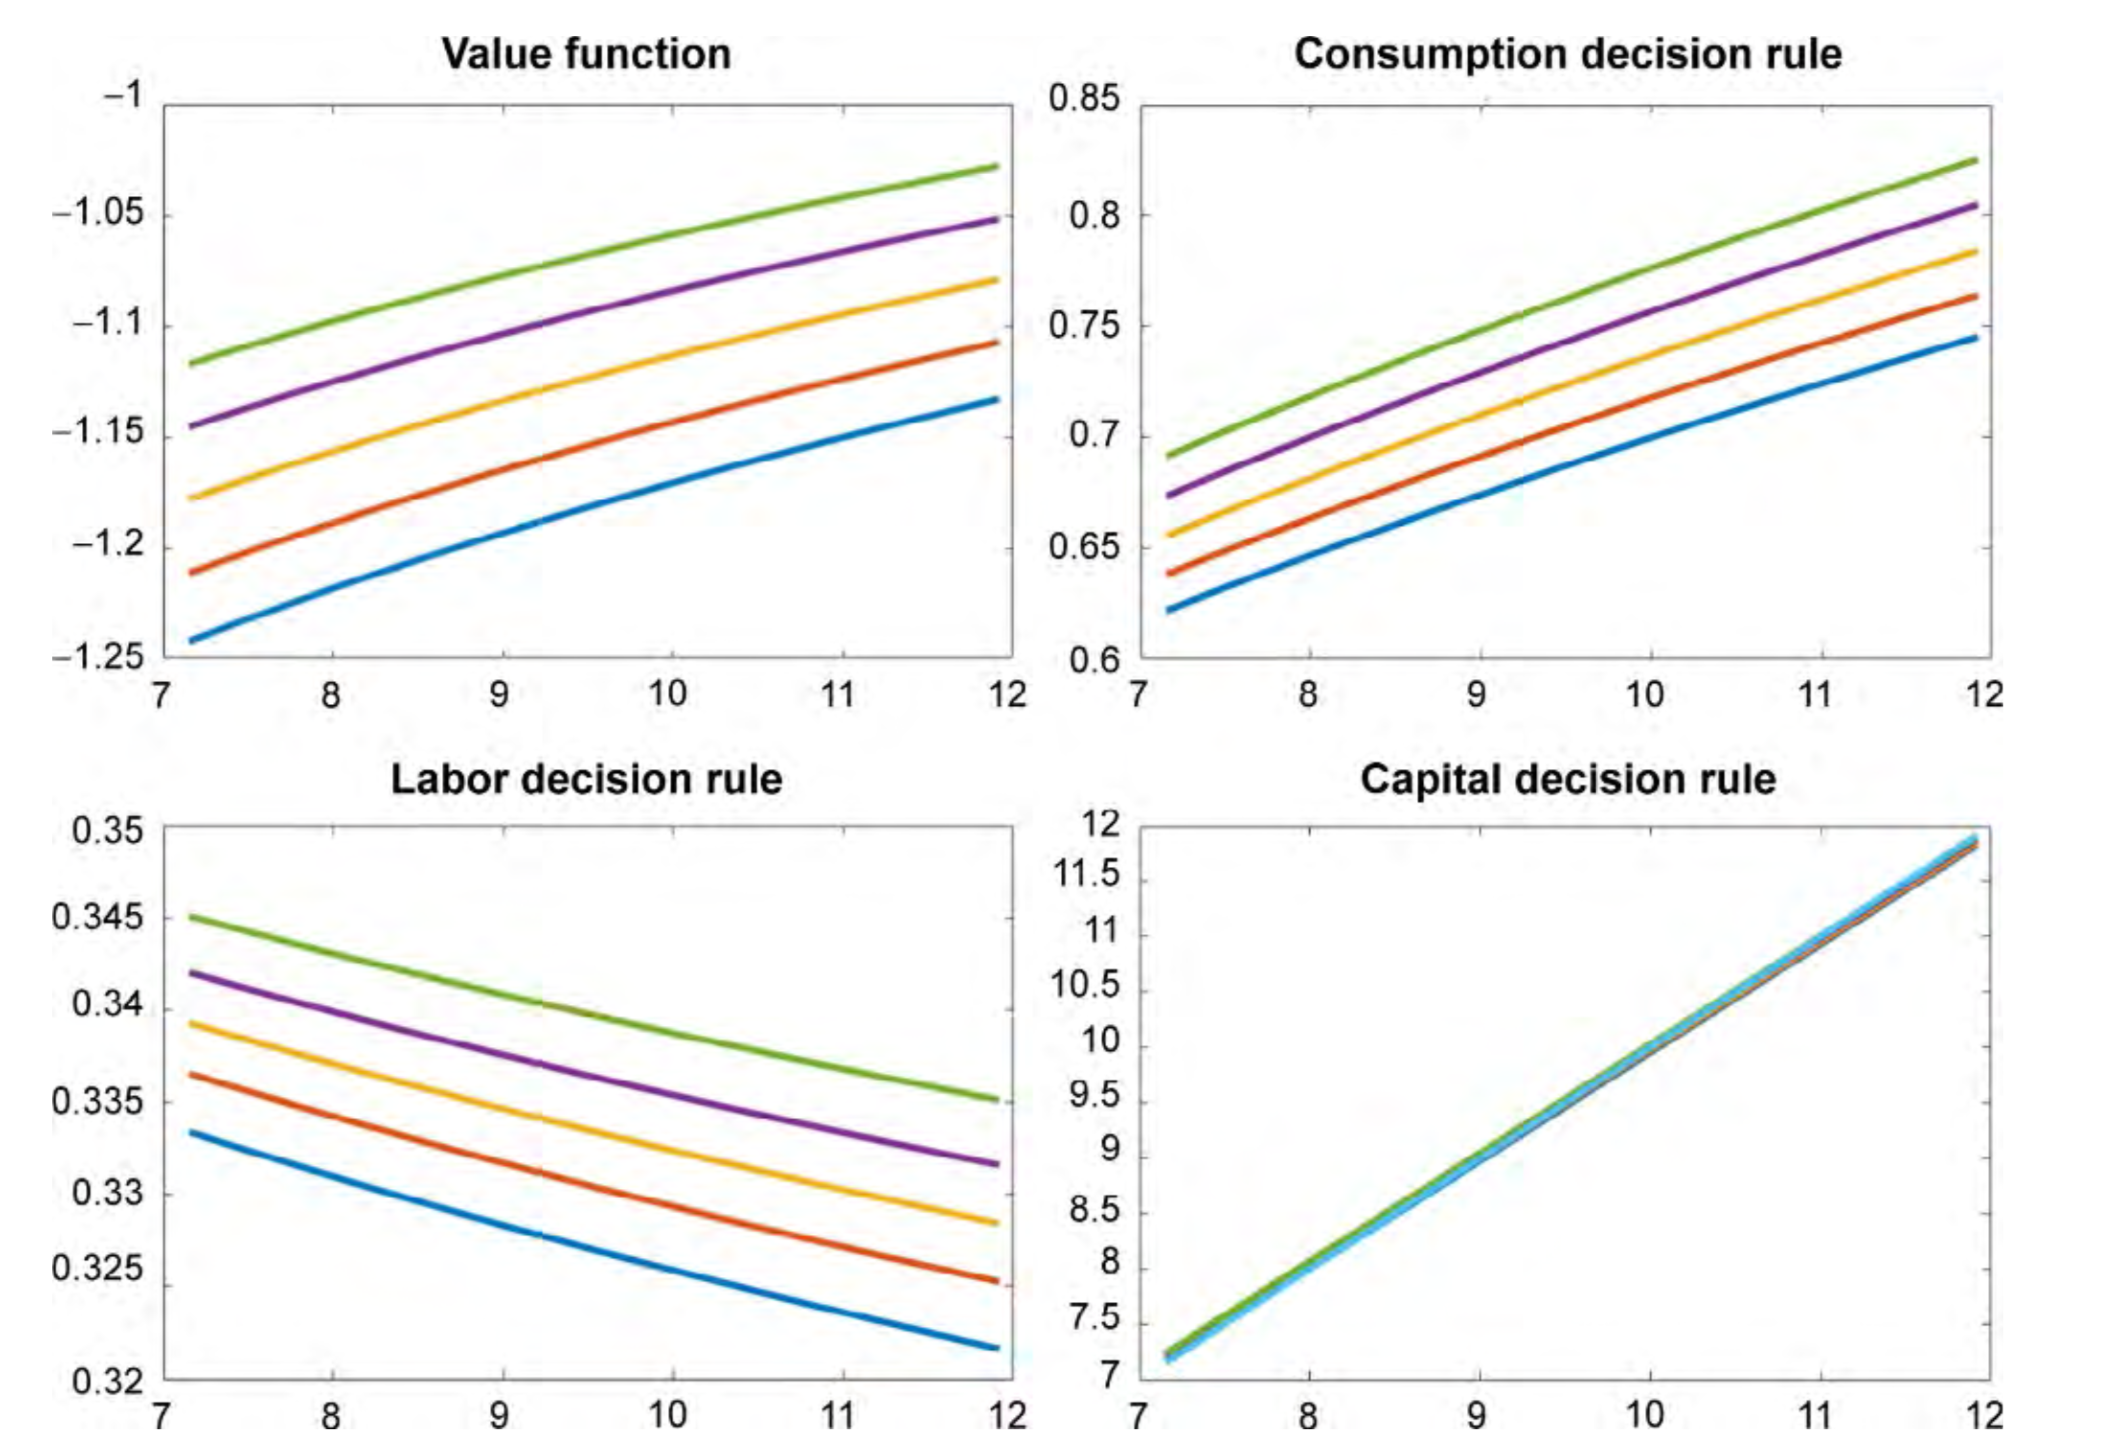
\includegraphics[width=12cm]{./Figures/20180325-projection-residual-analysis}
  \label{fig:pj-simulations-residual}
%
%  \small{Source: PBOC.}
\end{figure}

图\ref{fig:pj-simulations-residual}描述了用投影法求解随机新古典内生经济增长模型的模拟结果,从左上到右下分别表示价值方程的近似,消费、劳动力供应、资本积累决策方程的近似。五条颜色的线段分别表示5种技术冲击水平。横轴是状态变量$k_{t}$。
\begin{itemize}
  \item 价值方程的近似,符合模型设定,即价值方程是关于$k_{t}$和$z_{t}$的凹函数(concave)。
  \item 值得注意的是右下图,资本积累的决策方程,基本呈近似线性特征,这暗示着模型设定中资本积累式的线性型设定是比较合理的。
\end{itemize}

在求得1个价值方程和3个决策方程的近似式的基础上,我们便可以进一步对模型做仿真,计算冲击响应方程,并展开福利效果分析了。

投影法做近似求解可以达到非常高的精度,对误差项精度的进一步解读,可见下一节\todo{做一个ref}。总的说来,图\ref{fig:pj-simulations-residual}的近似解足以代替(离散生产率水平设定下的)新随机新古典主义增长模型的解析解。


\section{稀疏网格}
\label{sec:pj-sparsity}
高维DSGE模型的求解普遍受到维数灾难的限制,是公认难题。在利用完全多项式来近似求解高维系统的过程中,一种可以更好处理维数灾难的投影法是稀疏网格法(sparse grid)\index{sparse grid \dotfill 稀疏网格},又称Smolyak算法\index{Smolyak algorithm \dotfill Smolyak算法}。

数学上的Smolyak算法介绍,可见\cite{Smolyak:1963tu,Delvos:1982cg, Barthelmann:2000bq},一个全面的文献综述可见\cite{Bungartz:2004tc}。

\cite{Krueger:2004gh, Malin:2011hf}等首次尝试将Smolyak算法引入经济学研究中去,尤其是DSGE模型的求解。随后,一系列相关工作逐渐展开,如
\begin{enumerate}
  \item \cite{FernandezVillaverde:2015hs}利用Smolyak算法求解一个有着利率零下限设定的5个状态变量的新凯恩斯模型。
  \item \cite{FernandezVillaverde:2016wg}利用Smolyak算法求解一个存在大规模灾难性风险设定的12个状态变量的新凯恩斯模型。
  \item \cite{Gordon:2011ki}用Smolyak算法求解一个动态的异质行为人模型,异质性表现为总量层面上的分布方程,以一个状态变量直接进入模型当中。
  \item \cite{Malin:2011hf}对一个大规模、高度非线性DSGE模型做出精确估计,模型中含有20个连续状态变量。高度非线性表现一系列生产函数和效用函数的曲率上。
  \item  除了Smolyak算法之外,稀疏网格矩阵的另一种方法,是基于遍历集合(ergodic set)\index{ergodic set \dotfill 遍历集}来求解高维非线性系统,解释效果和精度也较为理想,可参考\cite{Maliar:2011jd,Judd:2011kb,Judd:2011iw}等。一个全面的介绍可见\cite{Maliar:2015fw}。
\end{enumerate}

这里以\cite{Krueger:2004gh, Malin:2011hf}为例,介绍用Smolyak算法求解DSGE模型的基本思路。研究的目标依旧是近似求解一个由$n$个状态变量构成的方程,如决策方程、价值方程、期望方程等,表示为\footnote{
两个简单的扩展:一是
\begin{equation*}
d: \left[ -k,k \right]^{n} \mapsto \left[ -1,1 \right]^{n}, \, k \neq 1,
\end{equation*}
可参考如第\ref{sec:pj-sparsity-steps-interval}节。二是
\begin{equation*}
  d: \left[ -k,k \right]^{n} \mapsto \mathrm{R}^{m}, \, m \neq n, m >0, n > 0.
\end{equation*}

}
\begin{equation*}
  d: \left[ -1,1 \right]^{n} \mapsto \mathrm{R}^{m}.
\end{equation*}

Smolyak算法的求解思路为,找到一个由若干点组成的网格$\mathrm{G}(q,n), \, q > n$,以及一个近似方程$d \left( x | \theta, q, n\right):\left[ -1, 1 \right]^{n} \mapsto \mathrm{R}$,这个近似方程由系数向量$\theta$予以描述,使得
\begin{itemize}
  \item 在网格$\mathrm{G}(q,n)$中的任意一点$x_{i} \in \mathrm{G}(q,n)$,待求解的未知方程$d(\cdot)$和近似方程$d \left( \cdot | \theta, q , n \right)$相等,即$\mathcal{H} \left( \cdot \right)$算子得到充分满足
  \begin{equation*}
    d \left( x_{i} \right) = d \left( \cdot | \theta, q , n \right), \, \forall \, x_{i} \in \mathrm{G}(q,n).
  \end{equation*}
  \item 在不属于网格的点$x_{i} \notin \mathrm{G}(q,n)$,近似方程$d \left( \cdot | \theta, q , n \right)$接近原方程$d \left( \cdot \right)$,即残差接近于$0$。
\end{itemize}

不难看出,$q$的作用在于描述网格的大小,以及衡量近似解的精确程度。

Smolyak算法的核心在于,如何选取恰当的网格$\mathrm{G}(q,n)$,以确保系数向量$\theta$不会随着$n$而爆炸。

Smolyak编程较难,但有突出优点:
\begin{itemize}
  \item 在多种基于多项式近似的算法中,它(几乎)是最优的算法\citep{Barthelmann:2000bq},
  \item 它提供全局解,即对许多方程空间来说都(几乎)是普遍最优的。
\end{itemize}

\subsection{Smolyak法的步骤}
\label{sec:pj-sparsity-steps}
如上文所述,Smolyak算法的核心是选定适宜的稀疏网格$\mathrm{G}(q,n)$和近似方程$d \left( \cdot | \theta, q, n\right)$。以下是常见步骤。

\subsubsection{状态变量的域转换}
\label{sec:pj-sparsity-steps-interval}
任意状态变量$\left\{ \tilde{x}_{\ell} \right\}_{\ell = 1}^{n}: \left[ a, b \right]^{n}$,可用如下方法线性平移至单位域$[-1,1]^{n}$中,变为$\left\{ x_{\ell} \right\}_{\ell = 1}^{n}: \left[ -1, 1 \right]^{n}$:
\begin{equation}
  \label{eq:pj-sparsity-steps-interval}
  x_{\ell} = 2 \frac{\tilde{x}_{\ell} - a}{b-a} -1, \quad \ell = 1, \ldots, n.
\end{equation}

\subsubsection{状态变量的域转换}
\label{sec:pj-sparsity-steps-poly-order}
定义多项式的阶,$m_{i}, i=1,2,\ldots$从而在随后的步骤中,用$m_{i-1}$阶多项式来近似原方程$d(\cdot)$:
\begin{equation}
  \label{eq:pj-sparsity-steps-poly-order}
  m_{i} = \begin{cases}
  1 & i = 1, \\
  2^{i-1} +1, & i=2,3,\ldots
  \end{cases}
\end{equation}

\subsubsection{建立克伦肖——柯蒂斯结点}
\label{sec:pj-sparsity-steps-cc-nodes}
构建复数集合$\mathrm{g}^{i} = \left\{ \xi_{1}^{i}, \ldots, \xi_{m_i}^{i} \right\} \subset \left[ -1 , 1 \right]$,每个上角标为$i$的集合中都包含有$m_{i}$个克伦肖——柯蒂斯结点(Clenshaw-Curtis nodes, \index{Clenshaw-Curtis Rule \dotfill 克伦肖——柯蒂斯求积法则}见第\ref{sec:ninc-cc-quadrature-rule}节)。
$\xi_{j}^{i}, \, j=1,2,\ldots, m_{i}$的值是切比雪夫多项式\eqref{eq:poly-chebyshev-1-def},取值范围在上下极值(extrema)$\left[ -1, 1 \right]$之间,满足
  \begin{equation}
    \label{eq:pj-sparsity-cc-nodes}
    \xi_{j}^{i} = - \cos \left( \frac{j - 1}{m_{i}-1}\right) \pi, \quad j = 1,\ldots,m_{i}.
  \end{equation}

  举例来说,\begin{itemize}
  \item 当$i=1$时,$m_{1}=1$,初始集合设为$\mathrm{g}^{1} = \left\{ \xi^{1} \right\} = \left\{ 0 \right\}$,只有一个值。
  \item 当$i=2$时,$m_{2} = 3$,3阶切比雪夫多项式构成$\mathrm{g}^{2} = \left\{ -1, 0, 1 \right\}$。
  \item 当$i=3$时,$m_{2} = 5$,$\mathrm{g}^{2} = \left\{ -1, - \cos \left( \frac{\pi}{4} \right), 0, - \cos \left( \frac{3 \pi}{4} \right), 1 \right\}.$
  \item 当$i=4$时,$m_{4} = 9$,$\mathrm{g}^{4} = \left\{ -1, -\cos \frac{\pi}{8}, -\cos \frac{\pi}{4}, -\sin \frac{\pi}{8}, 0, \sin \frac{\pi}{8}, - \cos \frac{3}{4} \pi, \cos \frac{\pi}{8}, 1 \right\}$,
\end{itemize}
以此类推。可见随着$i$的逐渐增加,$m_{i}$指数增加,集合$\mathrm{g}^{i-1}$中的值都包含在了$\mathrm{g}^{i}$中。(向下兼容性)。这个性质对Smolyak算法来说至关重要。

\subsubsection{构建稀疏网格}
\label{sec:pj-sparsity-steps-sparse-grid}
给定系统中状态变量的数量$n$,对于任意$q > n, q \in \mathcal{Z}$,可将稀疏网格$\mathrm{G} \left( q,n \right)$定义为一个由一系列笛卡尔乘积(cartesian product)\index{cartesian product \dotfill 笛卡尔乘积}所组成的并集
\begin{equation*}
  \mathrm{G} \left( q,n \right) = \bigcup_{q-n+1 \le \left| \Upsilon \right| \le q} \left( \mathrm{g}^{i_1} \times \mathrm{g}^{i_2} \times \ldots \times \mathrm{g}^{i_n}\right), \quad \left| \Upsilon \right| \equiv \sum_{\ell=1}^{n} i_{\ell}.
\end{equation*}

以一个$n=2$个连续状态变量的DSGE模型为例,我们选取$q=3$,那么稀疏网格
\begin{equation*}
  \begin{split}
    \mathrm{G} \left( 3, 2 \right)
    & = \bigcup_{2 \le \left| \Upsilon \right| < 3} \left( \mathrm{g}^{i_1} \times \mathrm{g}^{i_2} \right) \\
    & = \left( \mathrm{g}^{1} \times \mathrm{g}^{1} \right)
    \cup
    \left( \mathrm{g}^{1} \times \mathrm{g}^{2} \right)
    \cup
    \left( \mathrm{g}^{2} \times \mathrm{g}^{1} \right) \\
    & = \left\{ (-1,0), (0,1), (0,0), (0,-1), (1,0) \right\},
  \end{split}
\end{equation*}
将这些坐标绘制出来,见图\ref{fig:pj-sparse-grid-example}左上角。

\begin{figure}[htbp]
   \caption[稀疏网格]{稀疏网格$\mathrm{G}(3,2),\mathrm{G}(4,2),\mathrm{G}(5,2),\mathrm{G}(6,2)$}
  \centering
  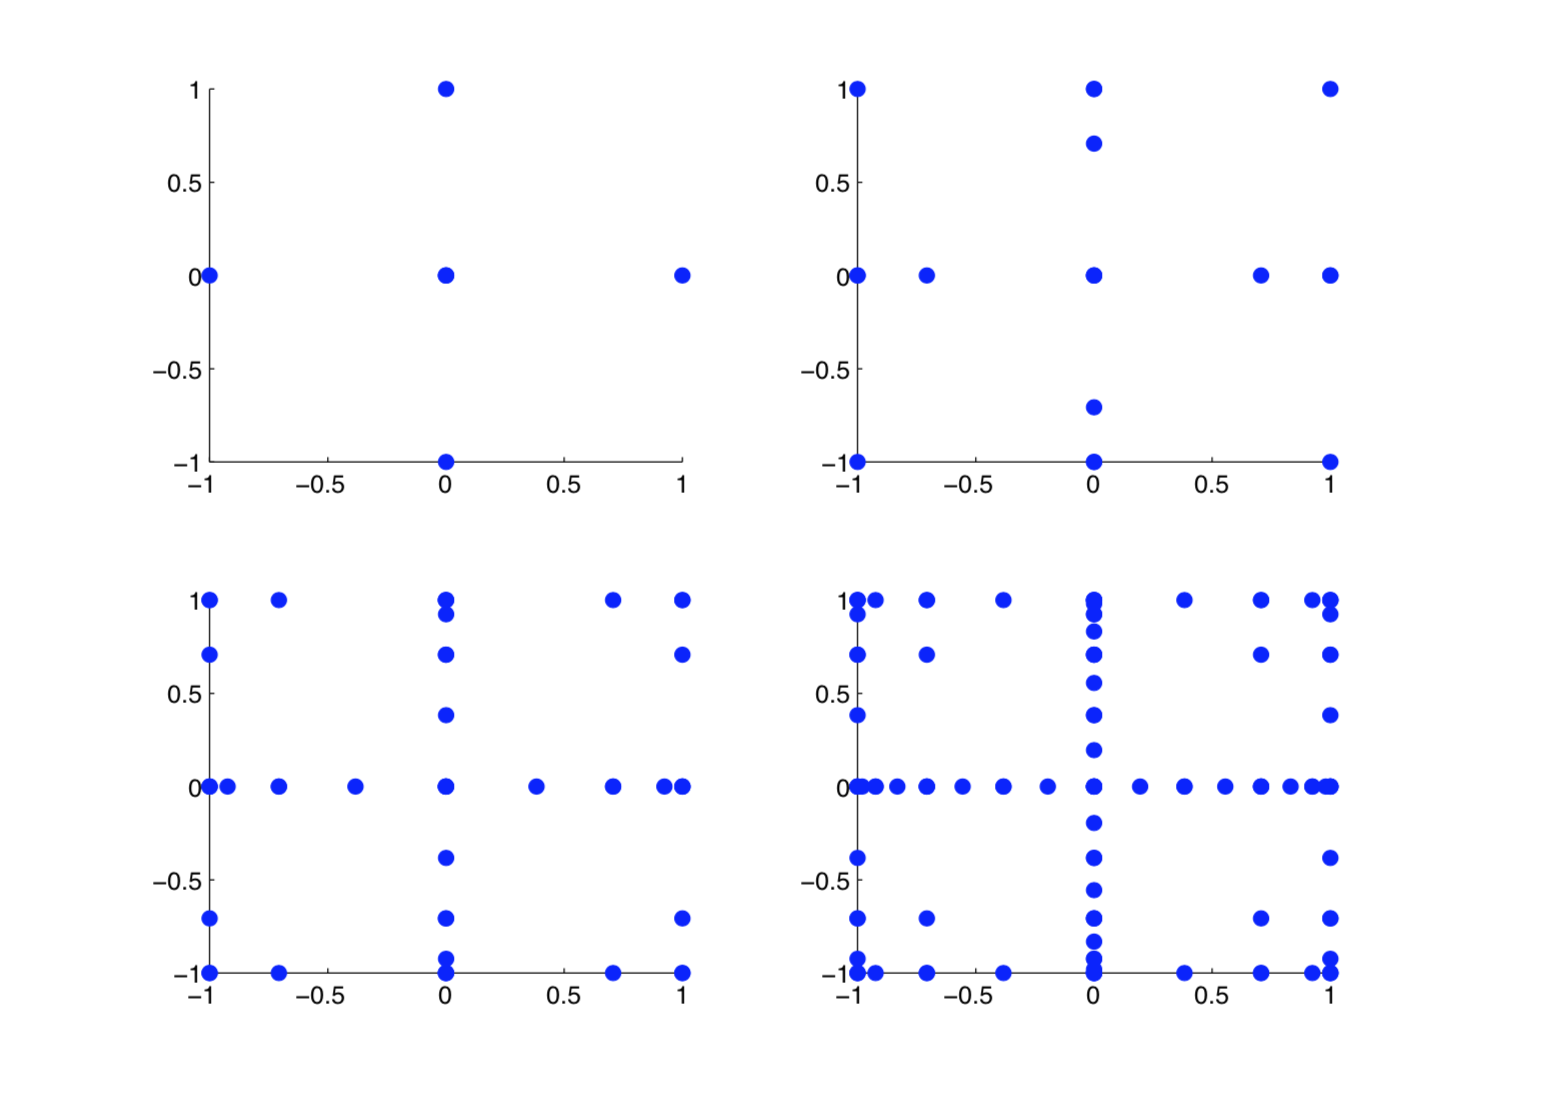
\includegraphics[width=12cm]{./Figures/20180325-sparse-grid-example}
  \label{fig:pj-sparse-grid-example}

  \small{来源: \cite{Krueger:2004gh} Figure 1。}
\end{figure}

如果选$q=4$,那么
\begin{equation*}
  \begin{split}
    \mathrm{G} \left( 4, 2 \right)
    = & \bigcup_{3 \le \left| \Upsilon \right| < 4} \left( \mathrm{g}^{i_1} \times \mathrm{g}^{i_2} \right) \\
    = & \left( \mathrm{g}^{1} \times \mathrm{g}^{2} \right)
    \cup
    \left( \mathrm{g}^{1} \times \mathrm{g}^{3} \right)
    \cup
    \left( \mathrm{g}^{2} \times \mathrm{g}^{2} \right)
    \cup
    \left( \mathrm{g}^{3} \times \mathrm{g}^{1} \right)\\
    = & \left\{
    (-1,-1),(-1,0),(-1,1),
    \left( -\cos\frac{3}{4}\pi, 0 \right),
    \left( -\cos\frac{1}{4}\pi, 0 \right), \right.\\
    & \left. (0,-1), \left(0, -\cos\frac{3}{4}\pi \right), \left(0, -\cos\frac{1}{4}\pi \right), (0,0), (0,1),
    (1,-1), (1,0), (1,1)
    \right\},
  \end{split}
\end{equation*}
坐标对应图\ref{fig:pj-sparse-grid-example}右上角。以此类推,图\ref{fig:pj-sparse-grid-example}的左下、右下分别绘出$\mathrm{G} \left(5,2 \right)$和$\mathrm{G} \left(6,2 \right)$的坐标。
$\mathrm{G} \left( 5,3 \right)$的网格点,见图\ref{fig:pj-sparse-grid-example-g53}。
\begin{figure}[htbp]
   \caption{稀疏网格$\mathrm{G}(5,3)$}
  \centering
  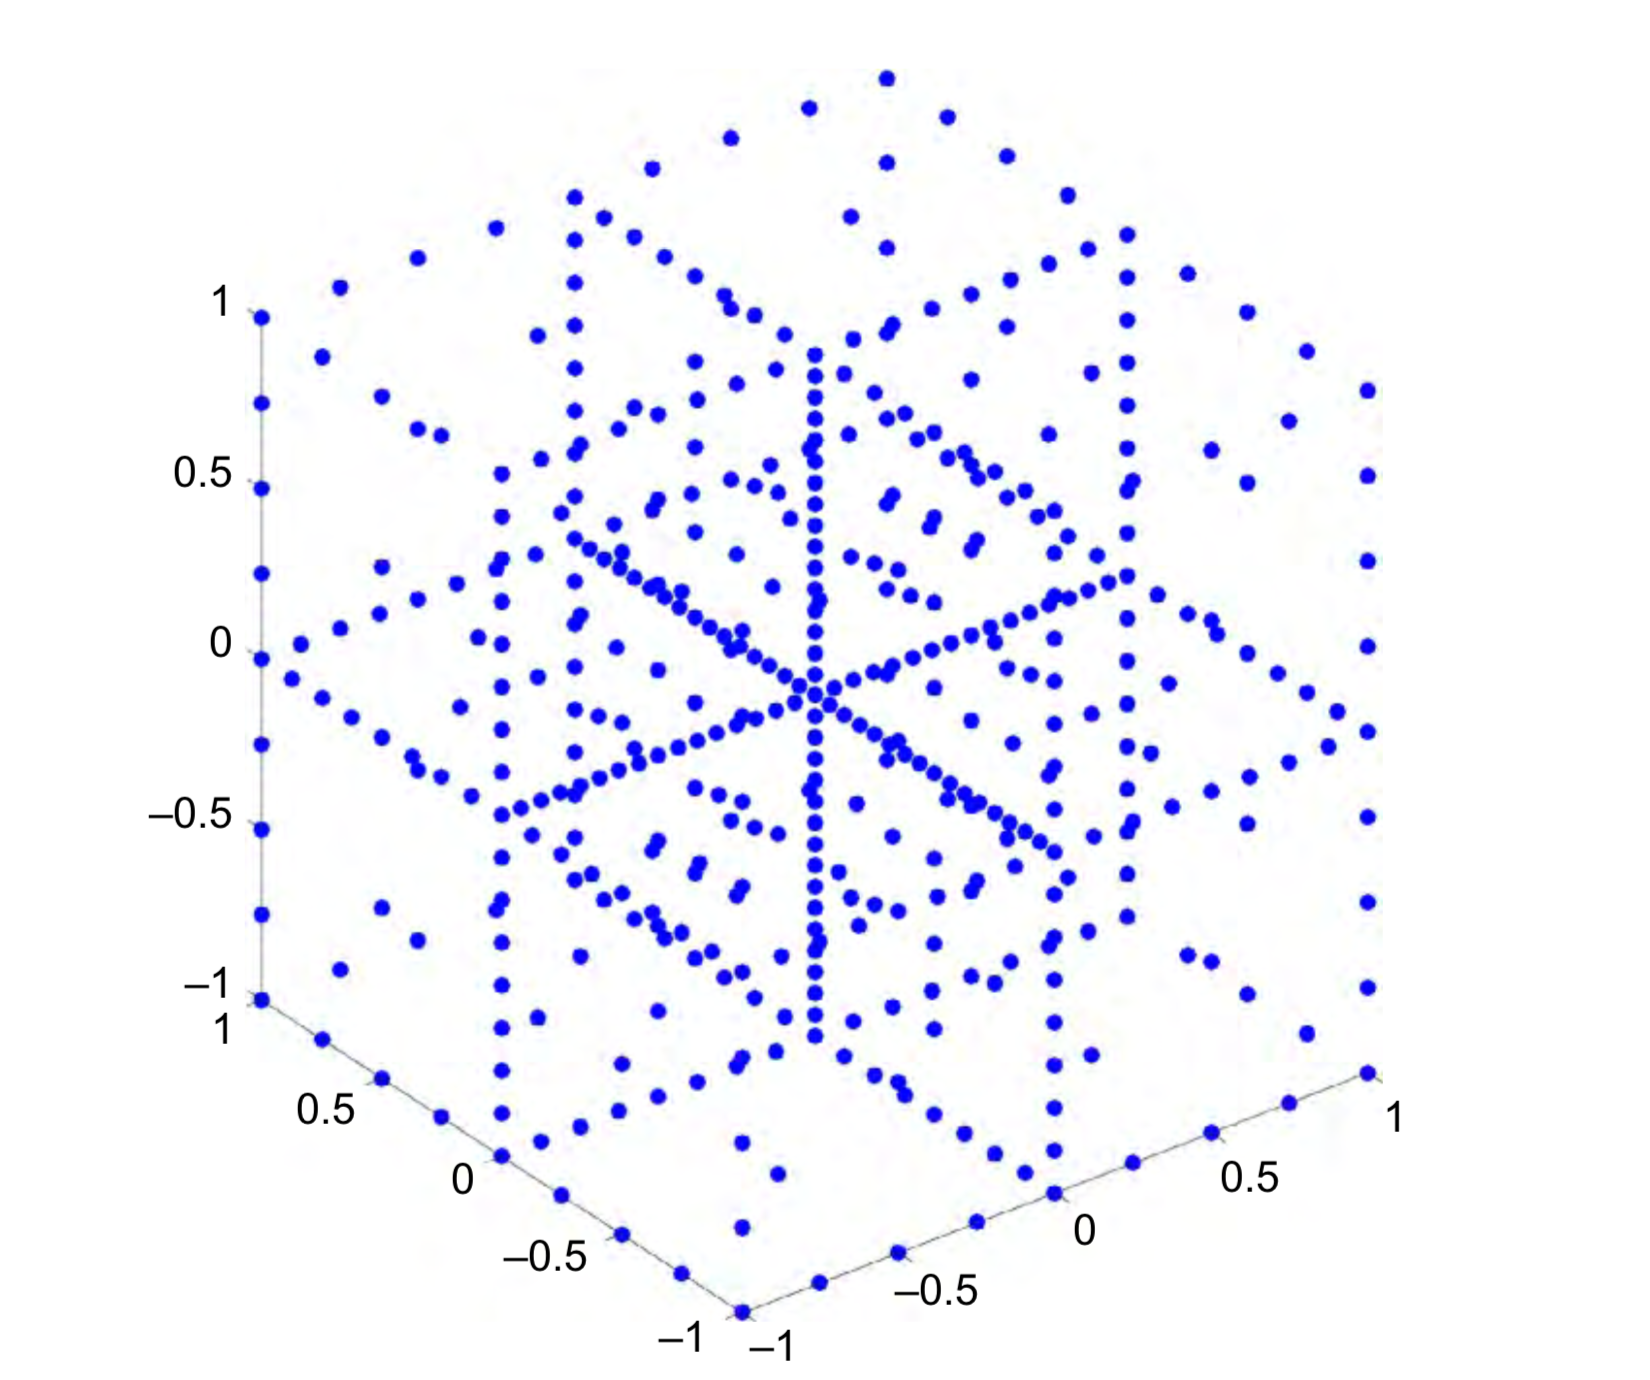
\includegraphics[width=12cm]{./Figures/20180325-sparse-grid-G53}
  \label{fig:pj-sparse-grid-example-g53}
  %
  %\small{来源: \cite{Krueger:2004gh} Figure 1。}
\end{figure}

从图\ref{fig:pj-sparse-grid-example}和\ref{fig:pj-sparse-grid-example-g53}不难看出稀疏网格的两个重要特征:
\begin{enumerate}
  \item 网格点在全部值域空间中的分布是不均匀的,越是靠近边缘的地区,和越是靠近域中心的位置,网格点越是密集。
  \item 一个$q=n+2$的稀疏网格中,有网格点数$2n(n-1)+4n+1$个。总结一般规律:网格$\mathrm{G}(q,n)$的势(cardinality)\index{cardinality \dotfill 势}随着$n^{2}$而呈多项式级数型增长。若$q = n+3$,则势随$n^{3}$呈多项式技术型增长。事实上在给定$n$不变的情况下,$q-n$的值越大,对应的网格点越多,数值求解越耗费资源。

  幸运的是,对大多数DSGE系统而言,$q=n+2$或者$q=n+3$就足以达到较为理想的近似精度了。
\end{enumerate}

在构建稀疏网格的过程中,之所以选用切比雪夫结点构建网格点的集合,是因为在克伦肖——柯蒂斯求积过程中,切比雪夫点具有很理想的嵌套性特征(nestedness)\index{nestedness of Chebyshev nodes \dotfill 嵌套性(切比雪夫结点)},该特征对于将$card \left( \mathrm{G}(q,n)\right)$控制在可操作范围内来说至关重要。例如,矩形网格的节点数是$5^n$个,总点数随着系统维度$n$的增加而指数上升;若$n=2$,这意味着需要在$[-1,1]^{2}$的二维空间中绘制$25$个结点。而得益于切比雪夫结点的嵌套性,在部署Smolyak算法的过程中,我们只需要考虑全部25个结点中的13个就够了——网格变得``稀疏''了。随着$n$的变化,普通矩形网格点数和稀疏网格点数,如表\ref{tab:pj-sparsity-nodes-comp}所示,相对于普通网格(如矩形网格)的指数增速,稀疏网格在控制网格点数量的增加(势)上有很大优势。

\begin{table}[htbp]
  \label{tab:pj-sparsity-nodes-comp}
\begin{center}
    \scriptsize
    \def\arraystretch{1.2}
    \centering
    \caption{网格结点的数量比较}
    \begin{threeparttable}
    \begin{tabular}{lrr}
        \hline
        $n$ & $card \left( \mathrm{G} \right)$\tnote{*} & $5^{n}$ \tnote{**}\\
        \hline
        2 & 13 & 25 \\
        3 & 25 & 125 \\
        4 & 41 & 625 \\
        5 & 61 & 3125 \\
        12 & 313 & 244,140,625 \\
        \hline
    \end{tabular}
    \begin{tablenotes}
        %\singlespacing
        \footnotesize
        \item[*] \tiny{稀疏网格结点的势$card \left( \mathrm{G} \left( q,n) \right) \right), \, q=n+2$。}
        \item[**] \tiny{普通网格结点的势,等于$5^{n}$。}
    \end{tablenotes}
\end{threeparttable}
\end{center}
\end{table}

\subsubsection{构建张量积方程}
\label{sec:pj-sparsity-tensor-product}
我们将多元多项式的乘积简化表示为张量积(tensor product)的形式(第\ref{sec:pj-multidimen-tensor}节),记为$p^{\left| \Upsilon \right|} \left( x | \theta \right)$
\begin{equation*}
  p^{\left| \Upsilon \right|} \left( x | \theta \right)
  \equiv
  \sum_{\ell_{1} =1}^{m_{i_{1}}} \ldots \sum_{\ell_{n}=1}^{m_{i_{n}}}
  \left( \theta_{\ell_{1} \ldots \ell_{n}} \right)
  \left[
  \psi_{\ell_{1}} \left( x_{1} \right)
  \ldots \psi_{\ell_{n}} \left( x_{n} \right)
  \right],
\end{equation*}
其中
\begin{itemize}
  \item \begin{equation*}
  \left| \Upsilon \right| \equiv \sum_{\ell=1}^{n} i_{\ell},
  \end{equation*}
  \item \begin{equation*}
  x \in [-1,1], \quad x = \left\{ x_{1}, \ldots, x_{n} \right\},
  \end{equation*}
  \item $\theta$是含有全部系数的堆栈,
  \begin{equation*}
    \theta = \left\{ \theta_{\ell_{1}, \ldots \ell_{n}} \right\},
  \end{equation*}
  \item 设基方程$\psi_{i} \left( x_{i} \right)$等于上一阶的切比雪夫多项式\footnote{这里选取切比雪夫多项式作为基方程,是因为切比雪夫多项式已经成为Smolyak算法求解DSGE系统所普遍采用的准则了。但也有其他选取方式的有益尝试,例如\cite{Nobile:2008kv}将有限元和Smolyak方法相结合,把值域$\Omega$分为若干元,在每个元中构建局部基方程再做加权求和。},
  \begin{equation*}
    \psi_{i} \left( x_{i} \right) = T_{i-1} \left( x_{i} \right), \quad i=1,\ldots,n
  \end{equation*}
  其中根据切比雪夫多项式的性质,设初始点$T_{0}(x_{i}) =1$。
\end{itemize}

那么,对于一个$n=2, \, q=3$的DSGE系统而言,$\left| \Upsilon \right|=\left\{ 2 , 3 \right\}$,分两种情况。
\begin{equation*}
  \begin{split}
    p^{\left| \Upsilon \right|, \, i=1,2} =
    \begin{cases}
    p^{\left| 2 \right|} \left( x | \theta \right) =  p^{1,1} \left( x | \theta \right), \\
    p^{\left| 3 \right|} \left( x | \theta \right) =  p^{1,2} \left( x | \theta \right) + p^{2,1} \left( x | \theta \right),
     \end{cases}
  \end{split}
\end{equation*}
其中
\begin{equation*}
  \begin{split}
    & \begin{cases}
    i=1 \Rightarrow m_{1}=1, \\
    i=2 \Rightarrow m_{2}=3,
    \end{cases} \\
    & p^{1,1} \left( x | \theta \right) =
    \sum_{\ell_{1}=1}^{m_{1}} \ldots \sum_{\ell_{n}=1}^{m_{1}} \theta_{\ell_{1} \ell_{2}} \psi_{\ell_{1}} \left( x_{1} \right) \psi_{\ell_{2}} \left( x_{2} \right) = \theta_{11}, \\
    & p^{1,2} \left( x | \theta \right) =
    \sum_{\ell_{1}=1}^{m_{1}} \ldots \sum_{\ell_{n}=1}^{m_{2}} \theta_{\ell_{1} \ell_{2}} \psi_{\ell_{1}} \left( x_{1} \right) \psi_{\ell_{2}} \left( x_{2} \right)
     = \theta_{11} + \theta_{12} \psi_{2} \left( x_{2} \right)
     + \theta_{13} \psi_{3} \left( x_{2} \right), \\
     & p^{2,1} \left( x | \theta \right)
     = \sum_{\ell_{1} =1}^{m_{2}} \sum_{\ell_{n}=1}^{m_{1}} \theta_{\ell_{1} \ell_{2}} \psi_{\ell_{1}} \left(x_{1} \right) \psi_{\ell_{2}} \left(x_{2} \right)
     = \theta_{11} + \theta_{21} \psi_{2} \left( x_{1} \right) + \theta_{31} \psi_{3} \left(x_{1} \right) = \theta_{11} + \theta_{21} T_{1} \left( x_{1} \right) + \theta_{31} T_{2} \left( x_{1} \right).
  \end{split}
\end{equation*}

或者可以通过简化系数堆栈$\theta$,来进一步简化上式。对于任意一个网格中的点$k_{1}, \ldots, k_{n}$,有
\begin{equation}
  \label{eq:pj-sparsity-theta-tensor-expansion}
  \begin{split}
    \theta = \theta_{\ell_{1} \ldots \ell_{n}}
    = \frac{
    2^{n}
    }{
    \left( k_{1} - 1 \right) \ldots \left( k_{n} - 1 \right)
    }
    \frac{
    1
    }{
    c_{\ell_{1}} \cdot c_{\ell_{n}}
    }
    \sum_{j_{1} =1}^{k_{1}} \ldots \sum_{j_{n} =1}^{k_{n}}
    \frac{
    1
    }{
    c_{j_{1}} \cdot c_{j_{n}}
    }
    \left[
    \psi_{\ell_{1}} \left( \xi_{1} \right)
    \psi_{\ell_{d}} \left( \xi_{n} \right)
    \right]
    d \left( xi_{1}, \ldots, \xi_{n} \right),
  \end{split}
\end{equation}
其中
\begin{itemize}
  \item
  \begin{equation*}
  c_{j} =
  \begin{cases}
  2 & j=1, \\
  1 & \forall \, j=2,3,\ldots
  \end{cases}
  \end{equation*}
  \item $\xi_{k} \in \mathrm{g}^{i}$表示克伦肖——柯蒂斯结点,如式\eqref{eq:pj-sparsity-cc-nodes}。
\end{itemize}

不难看出,这种张量积的近似测算方法,本质上来说就是在值域中,以克伦肖——柯蒂斯结点作插值。

%!TEX root = ../DSGEnotes.tex
\begin{subappendices}

  \section{超几何方程}
  \label{sec:hypergeometricfunctions}
  \begin{definition}[超几何序列]
    一组序列$\{c_n\}$,如果$\frac{c_{n+1}}{c_{n}}$是一个关于$n$的有理方程,则我们称$\{c_n\}$是一个超几何序列(Hypergeometric Series)\index{hypergeometric!series \dotfill 超几何序列}。
  \end{definition}

以阶乘形式表示为
\begin{equation}
\label{eq:hgf-hgf-series-fact}
\frac{c_{n+1}}{c_{n}} = \frac{\left(n+a_1\right) \left(n+a_2\right) \ldots \left(n+a_p\right)}{\left(n+b_1\right) \left(n+b_2\right) \ldots \left(n+b_q\right)} \frac{z}{\left(n+1\right)}, \quad n=0,1,2\ldots,
\end{equation}
如果$z=1$,$\{c_n\}$又称首一超几何序列(monic hypergeometric series)\index{hypergeometric!series, monic \dotfill 首一超几何序列};如果$z \neq 1$,则称非首一超几何序列。分母中的$n+1$项可以是来自阶乘本身,也可以不是,对于后者的情况,我们也可以在分子中加入一个额外的$(n+a_i)$项予以调节,即选取一个$i \in 0,1 \ldots n+1$使得$a_i = 1$。

对\eqref{eq:hgf-hgf-series-fact}做迭代我们有
\begin{equation}
\label{eq:hgf-hgf-series-iteration}
c_n = \frac{\left(a_1\right)_n \left(a_2\right)_n \ldots \left(a_p\right)_n}{\left(b_1\right)_n \left(b_1\right)_n \ldots \left(b_q\right)_n} \frac{z^n}{n!} c_0,
\end{equation}
其中$n!$表示$n$的阶乘。 $\left(a_1 \right)_n$表示伯赫哈默尔符号(Pochhammer symbol)\index{Pochhammer symbol \dotfill 伯赫哈默尔符号}的定义如下
\begin{equation*}
  \left(a_1 \right)_n := \begin{cases}
  1 & \quad \text{如果 } n=0,\\
   a_1 (a_1 + 1) (a_1 + 2) \ldots (a_1 + n -1) & \quad \text{如果 }n=1,2,3 \ldots.
  \end{cases}
\end{equation*}

对超几何序列$\{c_n\}$的求和为
\begin{equation*}
  \sum_{n=0}^{\infty} c_n = c_0 \sum_{n=0}^{\infty}  \frac{\left(a_1\right)_n \left(a_2\right)_n \ldots \left(a_p\right)_n}{\left(b_1\right)_n \left(b_1\right)_n \ldots \left(b_q\right)_n} \frac{z^n}{n!},
\end{equation*}
这引出超几何方程的定义。

\begin{definition}[超几何方程]
  超几何方程(hypergeometric function)\index{hypergeometric!function \dotfill 超几何方程}$\Hypergeometric{p}{q}{a}{b}{x}$定义为超几何序列$\{c_n\}$的和:
  \begin{equation}
    \label{eq:hgf-hgf-function}
    \Hypergeometric{p}{q}{a}{b}{x} = \sum_{k=0}^{n} c_n = \sum_{n=0}^{\infty} \frac{\left(a_1\right)_n \left(a_2\right)_n \ldots \left(a_p\right)_n}{\left(b_1\right)_n \left(b_1\right)_n \ldots \left(b_q\right)_n} \frac{z^n}{n!}
  \end{equation}
\end{definition}
显然,上式成立要求分母的系数$\neq 0$。对于分子的系数,如果某一个$i$次系数$a_i=-N$,其中$N$是个非负整数,那么超几何方程$\Hypergeometric{p}{q}{a}{b}{x}$是一个关于$z$的多项式, 详见定义\ref{definition:hgf-generalized-definition};反之,则超几何序列的收敛速度$\rho$满足
\begin{equation*}
  \rho = \begin{cases}
  \infty &\quad \text{ 如果 } \,p < q+1, \\
  1 &\quad \text{ 如果 }\,p = q+1,\\
  0 &\quad \text{ 如果 }\,p > q+1,
  \end{cases}
\end{equation*}
这是由超几何序列的性质所决定的:由\eqref{eq:hgf-hgf-series-fact}可得
\begin{equation*}
  \lim_{n \rightarrow \infty} \left| \frac{c_{n+1}}{c_{n}} \right|= \begin{cases}
  \infty & \quad \text{ 如果 }\, p < q+1, \\
  \left| z \right| &\quad \text{ 如果 }\,p = q+1,\\
  \infty &\quad \text{ 如果 }\,p > q+1,
  \end{cases}
\end{equation*}
我们最为关注$p=q+1$的情况:随着$\left| z \right|$的取值不同,超几何函数$\Hypergeometric{q+1}{q}{a}{b}{z}$呈现出不同的收敛特点:
\begin{equation*}
  \Hypergeometric{q+1}{q}{a}{b}{z} \begin{cases}
  \text{收敛,} & \quad \text{如果}\, \left| z \right| < 1,\\
  \text{收敛,} & \quad \text{如果}\, \left| z \right| = 1, Re \left( \sum^{q} b_i - \sum^{q+1} a_j \right) >0,\\
  \text{有条件收敛,} & \quad \text{如果}\, \left| z \right| = 1, z \neq -1, -1 < Re \left( \sum^{q} b_i - \sum^{q+1} a_j \right) \le 0, \\
  \text{不收敛,} & \quad \text{如果}\, Re \left( \sum^{q} b_i - \sum^{q+1} a_j \right) \le -1.
  \end{cases}
\end{equation*}

\begin{definition}[广义超几何方程]
  \label{definition:hgf-generalized-definition}
  广义超几何方程(generalized hypergeometric function)\index{hypergeometric!function, generalized \dotfill 广义超几何方程}是超几何方程的一种特殊形式,定义式为
  \begin{equation}
    \label{eq:hgf-generalized-definition}
    \Hypergeometric{2}{1}{a,b}{c}{z} = \sum_{n=0}^{\infty} \frac{\left( a \right)_n \left( b \right)_n}{\left( c \right)_n} \frac{z^n}{n!},
  \end{equation}
\end{definition}
其中如果$a=-N, \, N=0,1,2\ldots$,那么我们有
\begin{equation*}
  \left( a \right)_n = \left( -N \right)_n = \left( -N \right)\left( -N +1 \right) \left( -N +2 \right) \ldots \left( -N + n -1 \right) = 0, \, n=N+1, N+2, N+3 \ldots.
\end{equation*}
那么\eqref{eq:hgf-generalized-definition}变为
\begin{equation}
  \label{eq:hgf-generalized-definition-N}
  \Hypergeometric{2}{1}{-N,b}{c}{z} = \sum_{n=0}^{N} \frac{\left(-N \right)_n \left( b \right)_n}{\left( b \right)_n} \frac{z^n}{n!}, \quad N=0,1,2 \ldots.
\end{equation}

如果${a_n}$不是个常数,那么超几何序列想要获得收敛特性,需要满足如下情况,第一种情况是$\left| z \right| <1$,第二种情况是$\left| z \right| = 1$以及$Re(c-a-b) >0$。

许多函数都可以表示为超几何方程的形式。如
\begin{equation*}
  \ln(1+x) = \sum_{n=0}^{\infty} \frac{(-1)^n}{n+1} x^{n+1} = \sum_{n=0}^{\infty} \frac{(1)_n (1)_n}{(2)_n} \frac{(-1)^n x^{n+1}}{n!}= \sum_{n=0}^{\infty} \frac{n! \, n!}{(n+1)!} \frac{(-1)^n x^{n+1}}{n!} = x \, \pFq{2}{1}{1,1}{2}{-x},
\end{equation*}

\begin{equation*}
\begin{split}
  \arctan{x} &= \sum_{n=0}^{\infty} \frac{(-1)^n}{2n+1} x^{2n+1} = \sum_{n=0}^{\infty} \frac{\left(\frac{1}{2}\right)_n (1)_n}{\left(\frac{3}{2}\right)_n} \frac{(-1)^n x^{2n+1}}{n!} = x \, \pFq{2}{1}{\frac{1}{2},1}{\frac{3}{2}}{-x^2}, \\
  &\text{最后一个等式是由于}\frac{\left(\frac{1}{2}\right)_n}{\left(\frac{3}{2}\right)_n} = \frac{\frac{1}{2}\frac{3}{2} \ldots \frac{2n-1}{2}}{\frac{3}{2}\frac{5}{2} \ldots \frac{2n+1}{2}} = \frac{\frac{1}{2}}{\frac{2n+1}{2}} = \frac{1}{2n+1}
\end{split}
\end{equation*}

\begin{theorem}[二项式定理]
  作为超几何方程的特殊形式之一,可以写成如下形式,称为二项式定理(binomial theorem)\index{binomial theorem \dotfill 二项式定理}
  \begin{equation}
    \label{eq:hgf-binomial-theorem}
    \pFq{2}{1}{a,b}{b}{z}=\pFq{1}{0}{a}{\_}{z} = \sum_{n=0}^{\infty} \frac{(a)_n}{n!}z^n = \sum_{n=0}^{\infty} \begin{pmatrix} -a \\ n \end{pmatrix}\frac{(a)_n}{n!}(-z)^n = (1-z)^{-a}, \quad \left| z \right|<1.
  \end{equation}
\end{theorem}

以及还有一类特殊的超几何方程
\begin{equation}
  \pFq{0}{0}{\_}{\_}{z}=\sum_{t=0}^{\infty} \frac{z^n}{n!} = e^z, \quad z \in \mathbb{C}.
\end{equation}

以及当系数趋近于无穷时:
\begin{align*}
%  \begin{split}
    &\lim_{b \rightarrow \infty} \pFq{2}{1}{a,b}{c}{\frac{z}{b}} = \lim_{b \rightarrow \infty} \sum_{n=0}^{\infty} \frac{(a)_n z^n}{(c)_n n!} \frac{(b)_n}{b^n} = \sum_{n=0}^{\infty} \frac{(a)_n}{(c)_n} \frac{z^n}{n!} = \pFq{1}{1}{a}{c}{z}, \\
    &\lim_{c \rightarrow \infty} \pFq{2}{1}{a,b}{c}{cz} =
    \lim_{c \rightarrow \infty} \sum_{n=0}^{\infty} \frac{(a)_n (b)_n}{n!} z^n \frac{c^n}{(c)_n} = \sum_{n=0}^{\infty} (a)_n \, (b)_n \, \frac{z^n}{n!} = \pFq{2}{0}{a,b}{\_}{z}.
%    \end{split}
\end{align*}

\begin{theorem}[超几何方程与欧拉积分表达式的转换]
  如果$Re (c) > Re (b) > 0$,那么对于沿着从$1$到$\infty$实数轴展开的所有 $z \in \mathbb{C}$,满足$\arg t = \arg (1-t) = 0$并且$(1-z t)^{-a}$有主值(principal value)的条件\footnote{膏按:反正这一串前提限定条件我没看懂...我的理解是,经济学研究中,能够熟悉下面的转换公式就可以了——这真是一本不负责任的``讲义''啊...},我们可以将超几何方程转换为欧拉积分表达式(Euler's integral representation)\index{Euler integral representation \dotfill 欧拉积分表达式}
  \begin{equation}
    \label{eq:hgf-euler-integral-transformation}
    \pFq{2}{1}{a,b}{c}{z} = \frac{\Gamma(c)}{\Gamma(b) \Gamma(c-b)} \int_{0}^{1} t^{b-1} (1-t)^{c-b-1} (1-z t)^{-a} \, dt.
    \end{equation}
\end{theorem}
\begin{proof}
  假设$\left| z \right| <1$,那么由二项式定理\eqref{eq:hgf-binomial-theorem}可得
  \begin{equation*}
    (1-z t)^{- a} = \sum_{n=0}^{\infty} \frac{(a)_n}{n!} z^n t^n,
  \end{equation*}
  这表明
  \begin{equation*}
    \int_{0}^{t} t^{b-1} (1-t)^{c-b-1} (1-z t)^{-a} dt = \underbrace{\sum_{n=0}^{\infty} \frac{(a)_n}{n!} z^n t^n}_{\text{RHS甲}} \underbrace{\int_{0}^{t} t^{b-1} (1-t)^{c-b-1} dt}_{\text{RHS乙}},
  \end{equation*}
  RHS分为两部分。乙是一个贝塔积分(Beta integral)\index{Beta integral \dotfill 贝塔积分},满足条件\footnote{
  其中$\Gamma(\cdot)$是Gamma方程\index{Gamma function \dotfill{伽马方程}},是阶乘函数在实数与复数上的扩展,定义为
  \begin{equation*}
    \Gamma(a) =\begin{cases}
    (n-1)! & \text{n是正整数}, \\
    \int_0^{\infty} t^{a-1} \exp(-t)  \, dt & z \in \mathbb{C}, Re(c) >0.
    \end{cases}
  \end{equation*}
  }
  \begin{equation*}
    \int_{0}^{t} t^{b-1} (1-t)^{c-b-1} dt = B(n+b, c-b) = \frac{\Gamma(n+b) \Gamma(c-b)}{\Gamma(n+c)}.
  \end{equation*}
此外Gamm方程可以转换为Pochhammer符号\index{Pochhammer symbol \dotfill 伯赫哈默尔符号}的表达形式:
\begin{equation*}
  \frac{\Gamma(n+b)}{\Gamma(b)} = b (b+1) (b+2) \ldots (b + n - 1) = (b)_n,
\end{equation*}
那么
\begin{equation*}
  \frac{\Gamma(n+b) \Gamma(c-b)}{\Gamma(n+c)} = \Gamma(c-b) \frac{\Gamma(b)}{\Gamma(c)} \frac{(b)_n}{(c)_n},
\end{equation*}
作为RHS乙代回原式有
\begin{equation*}
\frac{\Gamma(c)}{\Gamma(b) \Gamma(c-b)} \int_{0}^{t} t^{b-1} (1-t)^{c-b-1} (1-z t)^{-a} \, dt = \sum_{0}^{\infty} \frac{(a)_n \, (b)_n}{(c)_n} \frac{z^n}{n!} = \pFq{2}{1}{a,b}{c}{z}.
\end{equation*}
\end{proof}

\begin{theorem}[欧拉积分表达式与高斯求和公式的转换]对于$Re(c-a-b)>0$,我们有欧拉积分表达式与高斯求和公式(Gauss summation formula)\index{Gauss summation formula \dotfill{高斯求和公式}}的转换
  \begin{equation}
    \label{eq:hgf-euler-gauss}
    \pFq{2}{1}{a,b}{c}{1}=\frac{\Gamma(c) \, \Gamma(c-a-b)}{\Gamma(c-a) \, \Gamma(c-b)}.
  \end{equation}
\end{theorem}
\begin{proof}
  假设$\lim_{z \rightarrow 1}$,通过\eqref{eq:hgf-euler-integral-transformation}我们有
  \begin{equation*}
    \begin{split}
      &\lim_{z \rightarrow 1}\pFq{2}{1}{a,b}{c}{z} \approx \pFq{2}{1}{a,b}{c}{1} = \frac{\Gamma(c)}{\Gamma(b) \, \Gamma(c-b)} \, \int_{0}^{1} t^{b-1} (1-t)^{c-a-b-1} \, dt \\
      &=\frac{\Gamma(c)}{\Gamma(b) \, \Gamma(c-b)} \, B(b,c-a-b) = \frac{\Gamma(c)}{\Gamma(b) \, \Gamma(c-b)} \, \frac{\Gamma(b) \Gamma(c-a-b)}{\Gamma(c-a)} = \frac{\Gamma(c) \Gamma(c-a-b)}{\Gamma(c-a) \Gamma(c-b)}.
    \end{split}
  \end{equation*}
\end{proof}

\begin{theorem}[高斯求和公式与朱世杰——范德蒙德求和公式的转换]
  当$a=-n, n \in \{0,1,2\ldots\}$(并且$\lim_{z \rightarrow 1}$)时,高斯求和公式\eqref{eq:hgf-euler-gauss}缩减成为朱世杰——范德蒙德求和公式(Chu-Vandermonde summation)\index{Chu-Vandermonde summation \dotfill 朱世杰——范德蒙德求和公式}
  \begin{equation}
    \pFq{2}{1}{-n,b}{c}{1}=\frac{(c-b)_n}{(c)_n}, n=0,1,2\ldots.
  \end{equation}
\end{theorem}
\begin{proof}
  \begin{equation*}
    \frac{\Gamma(c) \Gamma(c-a-b)}{\Gamma(c-a) \Gamma(c-b)} = \frac{\Gamma(c) \Gamma(c-b+n)}{\Gamma(c+n) \Gamma(c-b)} = \frac{(c-b)_n}{c(n)}.
  \end{equation*}
\end{proof}

\begin{theorem}[超几何方程与法夫转换公式]
  我们可以用欧拉积分表达式证明,超几何方程可以写成法夫转换公式(Pfaff's transformation formula)\index{Pfaff's transformation formula \dotfill 法夫转换公式}的形式
  \begin{equation}
    \label{eq:hpf-pfaff-trans}
    \pFq{2}{1}{a,b}{c}{z}=(1-z)^{-a} \pFq{2}{1}{a,c-b}{c}{\frac{z}{z-1}}.
  \end{equation}
\end{theorem}
\begin{proof}
  定义$t=1-s$,代入欧拉积分表达式\eqref{eq:hgf-euler-integral-transformation}我们有
  \begin{equation*}
    \begin{split}
      \pFq{2}{1}{a,b}{c}{z} &= \int_0^1 t^{b-1} (1-t)^{c-b-1} (1-z t)^{-a} \, dt \\
      &= - \int_0^1 (1-s)^{b-1} s^{c-b-1} (1-z + z s)^{-a} \, ds \\
      &= (1-z)^{-a} \int_0^1 s^{c-b-1} (1-s)^{b-1} \left( 1 - \frac{z s}{z - 1} \right)^{-a} \, ds \\
      &= (1-z)^{-a} \pFq{2}{1}{a,c-b}{c}{\frac{z}{z-1}}.
    \end{split}
  \end{equation*}
\end{proof}

\begin{theorem}[超几何方程与欧拉转换公式]
  我们可以用法夫转换公式证明,超几何方程可以写成欧拉转换公式(Euler's transformation formula)\index{Euler transformation formula \dotfill 欧拉转换公式}的形式
  \begin{equation}
    \label{eq:hgf-euler-transformation-formula}
    \pFq{2}{1}{a,b}{c}{z} = (1-z)^{c-a-b} \pFq{2}{1}{c-a,c-b}{c}{z}.
  \end{equation}
\end{theorem}
\begin{proof}
  两次使用法夫转换公式
  \begin{equation*}
    \begin{split}
      \pFq{2}{1}{a,b}{c}{z} &= (1-z)^{a} \pFq{2}{1}{a,c-b}{c}{\frac{z}{z-1}} \\
      &= (1-z)^{a} (1-z)^{b-c} \pFq{2}{1}{c-a,c-b}{c}{\frac{\frac{z}{z-1}}{\frac{z}{z-1} - 1}}\\
      &=(1-z)^{c-a-b} \pFq{2}{1}{c-a,c-b}{c}{z}
    \end{split}
  \end{equation*}
\end{proof}

\begin{theorem}[法夫——萨尔舒茨求和公式]
  一个${}_{3}F_{2}$超几何方程又可以写成法夫——萨尔舒茨求和公式(Pfaff-Saalschütz summation formula)\index{Pfaff-Saalschütz summation formula \dotfill 法夫——萨尔舒茨求和公式}的形式
  \begin{equation}
    \label{eq:hgf-Pfaff-Saalschuetz}
    \pFq{3}{2}{-n,a,b}{c,1+a+b-c-n}{1} = \frac{(c-a)_n (c-b)_n}{(c)_n (c-a-b)_n}, \quad n=0,1,2\ldots.
  \end{equation}
\end{theorem}
\begin{proof}
  欧拉转换公式\eqref{eq:hgf-euler-transformation-formula}又可以写成
  \begin{equation*}
    (1-z)^{a+b-c} \pFq{2}{1}{a,b}{c}{z} = \pFq{2}{1}{c-a,c-b}{c}{z},
  \end{equation*}
  其中LHS$\rightarrow$
  \begin{equation*}
    \begin{split}
      (1-z)^{a+b-c} \pFq{2}{1}{a,b}{c}{z} &= \sum_{j=0}^{\infty} \frac{(c-a-b)_j}{j!} z^j \sum_{k=0}^{\infty} \frac{(a)_k (b)_k}{(c)_k} \frac{z^k}{k!} \\
      &=\sum_{n=0}^{\infty} \sum_{k=0}^{n} \frac{(a)_k (b)_k (c-a-b)_{n-k}}{(c)_k k! (n-k)!} z^n.
    \end{split}
  \end{equation*}
  RHS$\rightarrow$
  \begin{equation*}
    \pFq{2}{1}{c-a,c-b}{c}{z} = \sum_{n=0}^{\infty}
    \frac{(c-a)_n (c-b)_n}{(c)_n} \frac{z^n}{n!}.
  \end{equation*}

  比较两个式子中$z^n$对应的系数,我们有
  \begin{equation*}
    \sum_{k=0}^{n} \frac{(a)_k (b)_k (c-a-b)_{n-k}}{(c)_k k! (n-k)!} z^n = \frac{(c-a)_n (c-b)_n}{(c)_n n!}, \quad n=0,1,2 \ldots, \quad k\in \{0,1,2, \ldots n\}.
  \end{equation*}
\end{proof}

其中由于
\begin{align*}
  \frac{n!}{(n-k)!} = n(n-1)\ldots(n-k+1) = (-1)^k (-n) (-n+1) \ldots (-n + k -1) = (-1)^k (-n)^k,
\end{align*}
以及
\begin{align*}
  (c-a-b)_{n-k} &= \frac{
  (c-a-b)_n
  }{
  (c-a-b+n-k)(c-a-b+n-k-1)\ldots(c-a-b+n-1)
  } \\
  &=\frac{(c-a-b)_n}{(-1)^k (1+a+b-c-n)_k}.
\end{align*}

因此
\begin{equation*}
  \sum_{k=0}^{n} \frac{(a)_k (b)_k (-n)_{k}}{(c)_k k! (1+a+b-c-n)_k} = \frac{(c-a)_n (c-b)_n}{(c)_n (c-a-b)_n}, \quad n=0,1,2 \ldots, \quad k\in \{0,1,2, \ldots n\},
\end{equation*}
进而\eqref{eq:hgf-Pfaff-Saalschuetz}成立。

\begin{theorem}[法夫——萨尔舒茨求和公式与高斯求和公式的转换]
随着$n \rightarrow \infty$,${}_3{F}_{2}$的法夫——萨尔舒茨求和公式\eqref{eq:hgf-Pfaff-Saalschuetz}逐渐缩减到${}_2{F}_{1}$的高斯求和公式\eqref{eq:hgf-euler-gauss}的形式
\begin{equation}
  \label{eq:pfaff-schuetz-gauss-transform}
  \lim_{n\rightarrow \infty} \pFq{3}{2}{-n,a,b}{c,1+a+b-c-n}{1}=\pFq{2}{1}{a,b}{c}{1}.
\end{equation}
\end{theorem}
\begin{proof}
  根据
  \begin{equation*}
    (a)_n = a (a+1) \ldots (a+n-1) = \frac{\Gamma(a+n)}{\Gamma(a)},
  \end{equation*}
  我们有
  \begin{equation*}
    \begin{split}
          \frac{(c-a)_n (c-b)_n}{(c)_n (c-a-b)_n} &= \frac{
          \Gamma(c-a+n) \Gamma(c-b+n) \Gamma(c) \Gamma(c-a-b)
          }{
          \Gamma(c-a) \Gamma(c-b) \Gamma(c+n) \Gamma(c-a-b+n)
          } \\
          &= \frac{\Gamma(c) \Gamma(c-a-b)}{\Gamma(c-a) \Gamma(c-b)}
          \underbrace{\frac{\Gamma(c-a+n) \Gamma(c-b+n)}{\Gamma(c+n) \Gamma(c-a-b+n)}},
    \end{split}
  \end{equation*}
  上式中下括号部分可由斯特灵公式(Stirling formula)近似:
  \begin{equation*}
    \lim_{n \rightarrow 0} \frac{\Gamma(c-a+n) \Gamma(c-b+n)}{\Gamma(c+n) \Gamma(c-a-b+n)} \sim n^{c-a+c-b-c-c+a+b} = n^0 = 1,
  \end{equation*}
  即
  \begin{equation*}
    \lim_{n \rightarrow \infty} \frac{(c-a)_n (c-b)_n}{(c)_n (c-a-b)_n} = \frac{\Gamma(c) \Gamma(c-a-b)}{\Gamma(c-a) \Gamma(c-b)},
  \end{equation*}
  由此得到
  \begin{equation*}
    \begin{split}
          \pFq{2}{1}{a,b}{c}{1}&=\lim_{n\rightarrow \infty}\pFq{3}{2}{-n,a,b}{c,1+a+b-c-n}{1}\\
          &=\lim_{n \rightarrow \infty} \frac{(c-a)_n (c-b)_n}{(c)_n (c-a-b)_n} \\
          &=\frac{\Gamma(c) \Gamma(c-a-b)}{\Gamma(c-a) \Gamma(c-b)}.
    \end{split}
  \end{equation*}
\end{proof}

\section{多项式}
\label{sec:poly}

\subsection{正交集}
数学意义上来说,正交(orthogonal)意味着垂直(perpendicular)。如,一个三维向量空间中的向量集$\{x,y,z\}$是正交的,意思就是说任意两个正交向量的点乘(dot product)都为零,$x.y=0,x.z=0,y.z=0$。因此我们又将$\{x,y,z\}$称为正交集合。在$\{x,y,z\}$构成的三维空间中,任何一点都可以表示为$x,y$或$z$向量中的一项——换句话说,$\{x,y,z\}$共同构成了一个三维空间的基(basis)。

如果$\{x,y,z\}$都是单位向量,则进一步称之为标准正交向量集。

\begin{definition}[黎曼——斯蒂尔杰斯积分]
  在区间$[a,b]$内,假定对于一个实变量$\lambda$的实函数$\alpha(\lambda)$,存在一个对应的实函数$f(\lambda)$,则黎曼——斯蒂尔杰斯积分(Riemann-Stieltjes integral)\index{Riemann-Stieltjes integral \dotfill 黎曼——斯蒂尔杰斯积分}$\int_{a}^{b} f(\lambda) \, d \alpha(\lambda)$描述了当将区间$[a,b]$分割为无限多个块(数量用$\pi$表示)时,下述和的极限值
\begin{equation}
  \label{eq:poly-riemann-sitltjes-def}
  \int_a^b f(\lambda) \, d \alpha(\lambda) = \sum_{\lambda_i \in \pi } f(c_i) \left( \alpha(\lambda_{i+1}) - \alpha(\lambda_{i})\right), \quad c_i \in [\lambda_{i+1}, \lambda_{i}].
\end{equation}
\end{definition}
黎曼——斯蒂尔杰斯积分值若要存在,需要$f(\cdot)$是连续方程,以及非递减方程$\alpha(\cdot)$在$[a,b]$中有界。

黎曼——斯蒂尔杰斯积分常常直接写作简化形式
\begin{equation}
  \label{eq:poly-riemann-sitltjes-def-simp}
  \int_a^b f(\lambda) w(\lambda) \, d \lambda,
\end{equation}
其中$w(\cdot)$称权重方程(weight function\index{weight function \dotfill 权重方程})。

\subsection{正交多项式}
任意一个无限多项式序列$\{p_{n}(\lambda)\}_{n=0}^{\infty}$向量(其中$p_{n}(\lambda)$表示其中的第n次多项式),都构成无限维度向量空间中的一个基。
\begin{definition}[正交多项式]
  如果一个多项式序列$\{p_n(\lambda)\}_{n=0}^{\infty}$ 在区间$(a,b)$中,关于权重方程$w(\lambda)$,满足如下关系,那么我们说它是正交多项式(orthogonal polynomial):
  \begin{equation}
    \label{eq:poly-orthogonal-poly-def}
    \int_a^b w(\lambda) p_m(\lambda) p_n(\lambda) d \lambda = h_n \delta_{mn}
  \end{equation}
\end{definition}
  \begin{itemize}
    \item $h_n$ 称范数(norm)\index{norm \dotfill 范数}  ,正交多项式$p(\lambda)$的范数也表示为$\left| p \right|$,定义为(具体细节见第\ref{sec:lp-norm}。)
    \begin{equation}
      \label{eq:poly-norm-def}
      h_n = \left| p_{n}(\lambda) \right| = \int_a^b w(\lambda) p_n(\lambda)^2 \, d x >0, n=0,1,2\ldots
    \end{equation}
    \item 权重方程$w(\lambda)$应当在$(a,b)$区间内连续且为正,以使矩(moment) $\mu_n$存在。
    \item 矩(moment)\index{moment \dotfill 矩} $\mu_n$定义为
    \begin{equation}
    \label{eq:poly-moment-def}
    \mu_n = \int_a^b w(x) \lambda^n \, d \lambda, \quad i=0,1,2\ldots
  \end{equation}
    \item $\delta_{mn}$是克罗内克(Kronecker product) \index{Kronecker product\dotfill 克罗内克乘积},表达如下关系
    \begin{equation}
      \label{eq:poly-kronecker}
      \delta_{m,n} = \begin{cases}
      0 & m \neq n, \\
      1 & m=n.
      \end{cases}
    \end{equation}
    \item 积分$\langle f, g \rangle$表示多项式$f$和$g$的内积(inner product)\index{inner product \dotfill 内积}
    \begin{equation}
      \label{eq:poly-inner-product-def}
      \langle p,q \rangle =
      \int_a^b w(\lambda) f(\lambda) g(\lambda) \, d \lambda.
    \end{equation}
    \item 区间$(a,b)$称正交区间(可以是一个无限区间,即$a \rightarrow -\infty, \, b \rightarrow +\infty$)。
  \end{itemize}

如果正交多项式$\{p_n(\lambda)\}_{n=0}^{\infty}$对于$k =0,1,2 \ldots n$都有$h_k = 1$,则称标准正交多项式(orthonormal polynomial)\index{polynomial!orthonormal \dotfill 标准正交多项式}。

如果第n次多项式$p_n(\lambda)=k_n \lambda^n + \chi$,其中$\chi$表示低于n次的其他项,并且对于每一个$n=0,1 \ldots $ 都有 $k_n = 1$,则称首一正交多项式(monic orthogonal polynomial)\index{polynomial!monic orthogonal \dotfill 首一正交多项式}。

标准正交多项式$p_n(\lambda)$和首一正交多项式$\hat{p}_n(\lambda)$之间可以相互转换(如见定理\ref{theorem:poly-orthonormal-recurrence-theorem})。
\begin{equation}
  \label{eq:poly-monic-orthonormal-transformation}
  \hat{p}_n(\lambda) = \frac{p_n(\lambda)}{\sqrt{\langle p_n(\lambda), p_n(\lambda)\rangle}}.
\end{equation}

我们可以根据格拉姆-施密特正交化过程(Gram-Schmidt orthogonality process)\index{Gram-Schmidt orthogonality process \dotfill 格拉姆-施密特正交化过程},把正交多项式序列$\{p_{n}(\lambda)\}_{n=0}^{\infty}$转化为正交集合。举例说明,取$w(\lambda)=1, \, (a,b)=(0,1), \, p_{0}(\lambda)=1$,求首一多项式序列$\{p_{n}(\lambda)\}$。

从序列$\{1,\lambda, \lambda^2 \ldots \}$开始。第一步求$p_1(\lambda)$
\begin{equation*}
  \begin{split}
    p_1(\lambda) &= \lambda - \frac{\langle \lambda, p_{0}(\lambda) \rangle}{\langle p_{0}(\lambda) \lambda, p_{0}(\lambda) \rangle} \, p_0(\lambda) \\
    &= \lambda - \frac{\langle \lambda,1 \rangle }{\langle 1,1 \rangle} \\
    &= \lambda - \frac{
    \int_0^1 w(\lambda) \left(\lambda  \cdot 1 \right) \, d \lambda
    }{
    \int_0^1 w(\lambda) \left(1 \cdot 1 \right) \, d \lambda
    }\\
    &= \lambda - \frac{1}{2}.
  \end{split}
\end{equation*}

  第一步求$p_2(\lambda)$
  \begin{equation*}
    \begin{split}
      p_2(\lambda) &= \lambda^2 - \frac{\langle \lambda^2, p_0(\lambda) \rangle}{\langle p_0(\lambda),p_0(\lambda)\rangle} \, p_0(\lambda)
      - \frac{
      \langle \lambda^2, p_1(\lambda) \rangle
      }{
      \langle p_1(\lambda),p_1(\lambda)\rangle
      } \, p_1(\lambda) \\
      &= \lambda^2 - \frac{
      \langle \lambda^2, 1 \rangle
      }{
      \langle 1,1 \rangle
      } -\frac{
      \langle \lambda^2, \lambda-\frac{1}{2} \rangle
      }{
      \langle \lambda-\frac{1}{2}, \lambda-\frac{1}{2} \rangle
      } \left(\lambda-\frac{1}{2} \right)\\
      &=\lambda^2 - \frac{\frac{1}{3}}{1} - \frac{\frac{1}{12}}{\frac{1}{12}} \left( \lambda - \frac{1}{2} \right) \\
      &=\lambda^2 - \lambda + \frac{1}{6}.
    \end{split}
  \end{equation*}

则$p_0(\lambda)=1$,$p_1(\lambda)= \lambda - \frac{1}{2}$,$p_2(\lambda)=\lambda^2 - \lambda + \frac{1}{6}$就是首一正交多项式在(0,1)区间内,对应权重方程$w(\lambda)=1$的前三项。以此类推,可以继续求得$p_3(\lambda),p_4(\lambda) \ldots$
\begin{equation*}
  \begin{split}
    &p_3(\lambda) = \lambda^3 - \frac{3}{2} \lambda^2 + \frac{3}{5}\lambda - \frac{1}{20}, \\
    &p_4(\lambda) = \lambda^4 - 2 \lambda^3 + \frac{9}{7}\lambda^2 - \frac{2}{7} \lambda + \frac{1}{70}, \\
    &p_5(\lambda) = \lambda^5 - \frac{5}{2} \lambda^4 + \frac{20}{9} \lambda^3 - \frac{5}{6} \lambda^2 + \frac{5}{42} \lambda - \frac{1}{252} \ldots
  \end{split}
\end{equation*}

根据\eqref{eq:poly-norm-def}计算$h_n$;与首一正交多项式$p_n(\lambda)$对应的正交多项式$q_n(\lambda)$由\eqref{eq:poly-monic-orthonormal-transformation}给出
\begin{equation*}
  \begin{split}
    &q_1(\lambda) = \frac{p_1(\lambda)}{\sqrt{h_1}} = 2\sqrt{3} \left( x - \frac{1}{2} \right), \\
    &q_2(\lambda) = \frac{p_2(\lambda)}{\sqrt{h_2}} = 6 \sqrt{5} \left( x^2 - x + \frac{1}{6} \right), \\
    &q_3(\lambda) = \frac{p_3(\lambda)}{\sqrt{h_3}} = 20 \sqrt{7} \left( \lambda^3 - \frac{3}{2} \lambda^2 + \frac{3}{5}\lambda - \frac{1}{20} \right) \ldots
  \end{split}
\end{equation*}






















\subsubsection{正定}
如果$\left| p \right| >0, \, \left| q \right| >0, \, \forall p,q \in \mathbb{P}$,则$<.,.>$是正定的。换句话说,内积是正定的充分必要条件为,它的汉克尔矩阵(Hankel moment matrix)\index{Hankel moment matrix \dotfill 汉克尔矩阵}的行列式为正
\begin{equation}
  \label{eq:poly-hankel-moment-matrix-def}
  \det
  \begin{pmatrix}
    \mu_0 & \mu_1 & \mu_2 & \dots &\mu_{k-1} \\
    \mu_1 & \mu_2 & \mu_3 & \dots & \mu_k \\
    \vdots & \ddots & & & \vdots \\
    \mu_{k-1} & \mu_k & \mu_{k+1} & \dots & \mu_{2k-2}
  \end{pmatrix} >0, k=1,2,\ldots
\end{equation}
其中$\mu_i$的定义如\eqref{eq:poly-moment-def}所示。

\begin{theorem}[正交多项式的存在性]
  如果某内积$\langle.,.\rangle$在$\mathbb{P}$中正定,那么有且只有一个首一正交的无限多项式与每一个$\alpha(\lambda)$相对应。
\end{theorem}
\begin{proof}
  略。
\end{proof}

\begin{theorem}[正交多项式的最小化特性]
  如果$q_k(\lambda)$是一个$k$次的首一多项式,则只有当$q_k$等于一个常数与另一个同样关于$\alpha(\lambda)$的多项式$p_k$的乘积时,以下最小值才存在
  \begin{equation*}
    \min_{q_k} \int_a^b q_k(\lambda)^2 \, d \alpha(\lambda).
  \end{equation*}
\end{theorem}
\begin{proof}
  略。
\end{proof}

\subsection{递推关系}
\begin{theorem}[首一正交多项式的三项递推关系]
  \label{theorem:poly-recurrence-relation}
  对于首一正交多项式序列$\{ p_{n} (\lambda) \}$而言,存在着系数$\alpha_k$和$\gamma_k$,$k=1,2,\ldots$,使得其满足三项递推关系(three-term recurrence relation)\index{three-term recurrence relation!monic polynomial \dotfill 三项递推关系(首一正交多项式)}
  \begin{equation}
    \label{eq:poly-monic-poly-recurrence-def}
    \begin{split}
      &p_{k+1}(\lambda) = \left( \lambda - \alpha_{k+1} \right) p_{k}(\lambda) - \gamma_k p_{k-1}(\lambda) , \quad k = 1,2,\ldots, \\
      &p_{-1}(\lambda) :=0, \, p_{0}(\lambda) = 1, \\
      &\text{其中} \quad \alpha_{k+1} = \frac{\langle \lambda p_k, p_k \rangle}{\langle p_k,p_k \rangle}, \, \gamma_k = \frac{\langle p_k,p_k \rangle }{ \langle p_{k-1},p_{k-1} \rangle}.
    \end{split}
  \end{equation}
\end{theorem}

\begin{proof}
  对于$k =1,2,\ldots$设
  \begin{equation*}
    F(\lambda) := p_{k+1}(\lambda) - (\lambda - \alpha_{k+1}) p_{k}(\lambda) + \gamma_k \, p_{k-1}(\lambda),
  \end{equation*}
  由$p_{k-1},p_k,p_{k+1}$都是首一多项式可得$F(\lambda) \in \mathbb{P}_{n}[\lambda]$。此外,由$p_{k-1},p_k,p_{k+1}$的正交特性,我们分三种情况展开分析。

  第一种情况,当$0 < l < k-1$时,有
  \begin{equation*}
    \begin{split}
      \langle F(\lambda), p_{l}(\lambda) \rangle
      &= \underbrace{\langle p_{k+1}(\lambda),p_{l}(\lambda)\rangle}_{=0}
      - \underbrace{\langle p_{k}(\lambda), \left( \lambda - \alpha_{k+1} \right)p_{l}(\lambda) \rangle}_{=0}
      + \underbrace{\langle \gamma_k p_{k-1}(\lambda), p_{l}(\lambda)\rangle}_{=0} =0,
    \end{split}
  \end{equation*}
  其中用到了$\langle \lambda p, q \rangle = \langle p, \lambda q \rangle$,以及$\langle p_k,p_l \rangle =0, \, \forall \, 0 < l < k-1$。

  第二种情况,当$l = k-1$时,有
  \begin{equation*}
    \begin{split}
      \langle F(\lambda), p_{l}(\lambda) \rangle &= \langle F(\lambda), p_{k-1}(\lambda) \rangle \\
      &= \underbrace{\langle p_{k+1}(\lambda), p_{k-1}(\lambda) \rangle}_{=0} - \langle p_{k}(\lambda), \left( \lambda - \alpha_{k+1} \right) p_{k-1}(\lambda) \rangle
      + \langle \gamma_k p_{k-1}(\lambda), p_{k-1}(\lambda) \rangle \\
      &= -\langle p_{k}(\lambda), \lambda p_{k-1}(\lambda) \rangle
      + \underbrace{\langle p_{k}(\lambda), \alpha_{k+1} p_{k-1}(\lambda) \rangle}_{=0}
      +\gamma_k \langle p_{k-1}(\lambda), p_{k-1}(\lambda) \rangle = 0,
    \end{split}
  \end{equation*}
  因此我们有
  \begin{equation*}
    \gamma_k = \frac{
    \langle p_{k}(\lambda), p_{k}(\lambda) \rangle
    }{
    \langle p_{k-1}(\lambda), p_{k-1}(\lambda) \rangle
    }.
  \end{equation*}
  第三种情况,当$l=k$时,有
  \begin{equation*}
    \begin{split}
      \langle F(\lambda), p_{l}(\lambda) \rangle &= \langle F(\lambda), p_{k}(\lambda) \rangle \\
      &=\underbrace{\langle p_{k+1}(\lambda), p_{k}(\lambda) \rangle}_{=0}
      + \langle \left( -\lambda + \alpha_{k+1} \right) p_{k}(\lambda), p_{k}(\lambda) \rangle
      + \underbrace{\langle \gamma_k p_{k-1}(\lambda), p_{k}(\lambda) \rangle}_{=0} \\
      &=- \langle \lambda p_{k}(\lambda),p_{k}(\lambda) \rangle
      + \alpha_{k+1} \langle p_{k}(\lambda),p_{k}(\lambda) \rangle =0,
    \end{split}
  \end{equation*}
  因此我们有
  \begin{equation*}
    \alpha_{k+1} = \frac{
    \langle \lambda p_{k}(\lambda), p_{k}(\lambda)\rangle
    }{
    \langle p_{k}(\lambda), p_{k}(\lambda) \rangle
    }.
  \end{equation*}
\end{proof}

\begin{theorem}[标准正交多项式的三项递推关系]
  \label{theorem:poly-orthonormal-recurrence-theorem}
  对于标准正交多项式$\{p_{n} (\lambda)\}$而言,存在着系数$\alpha_k$和$\beta_{k}$,$k=0, 1,2,\ldots $,使得其满足三项递推关系(three-term recurrence relation)\index{three-term recurrence relation!orthonormal polynomial \dotfill 三项递推关系(标准正交多项式)}
  \begin{equation*}
    \begin{split}
      &\sqrt{\beta_{k+1}} p_{k+1}(\lambda) = \left( \lambda -\alpha_{k+1} \right) - \sqrt{\beta_{k}} p_{k-1}(\lambda), \quad k=1,2,\ldots\\
      &p_{-1}(\lambda) := 0, \, p_0(\lambda) = \beta_0^{-\frac{1}{2}}, \, \beta_0 = \int_a^b \, d \alpha(\lambda), \\
      &\text{其中} \quad \alpha_{k+1} = \langle \lambda p_{k}, p_{k} \rangle , \, \beta_k \, \text{通过计算} \left| p_k \right|=1 \, \text{求得}.
    \end{split}
  \end{equation*}
\end{theorem}
\begin{proof}
  假定有一个首一正交多项式$\{p_k(\lambda)\}_{n=0}^{\infty}$满足三项递推关系\eqref{eq:poly-monic-poly-recurrence-def},那么根据\eqref{eq:poly-monic-orthonormal-transformation},对应的标准正交多项式$\{\hat{p}_n(\lambda)\}_{n=0}^{\infty}$满足
  \begin{equation*}
    \hat{p}_k(\lambda)=\frac{p_{k}(\lambda)}{\sqrt{\langle p_k,p_k \rangle}} = \frac{p_{k}(\lambda)}{\left| p_k \right|},
  \end{equation*}
  最后一个等号由\eqref{eq:poly-norm-def}-\eqref{eq:poly-inner-product-def}联立求得。上式代回\eqref{eq:poly-monic-poly-recurrence-def}可得
  \begin{equation*}
    \hat{p}_{k+1}(\lambda) \left| p_{k} \right|
    = \left(
    \lambda \left| p_{k+1} \right| - \frac{
    \langle \lambda p_k, p_k \rangle
    }{
    \left| p_k \right|
    }
    \right) \hat{p}_{k}
    - \left( \frac{\left| p_k \right| ^2}{\left| p_{k-1} \right|} \right)  \hat{p}_{k-1},
  \end{equation*}
  进一步整理
  \begin{equation*}
    \frac{\left| p_{k+1} \right|}{\left| p_k \right|} \hat{p}_{k+1} = \left( \lambda - \langle \lambda \hat{p}_k, \hat{p}_{k} \rangle \right) \hat{p}_k
    - \frac{\left| p_k \right|}{\left| p_{k-1} \right|} \hat{p}_{k-1},
  \end{equation*}
  由此我们有
  \begin{equation*}
    \langle \lambda \hat{p}_k, \hat{p}_k \rangle = \frac{
    \langle \lambda p_k, p_k \rangle
    }{\langle p_k, p_k \rangle} = \alpha_{k+1}, \quad \sqrt{\beta_{k+1}} = \frac{
    \langle p_{k+1}, p_{k+1} \rangle
    }{
    \langle p_k, p_k \rangle
    } = \gamma_{k+1}.
  \end{equation*}

  在求得首一多项式$\{ p_{n}(\lambda) \}_{n=0}^{\infty}$的三项递归关系系数$(\alpha_{k}, \gamma_k)$后,对应的标准多项式$\{ \hat{p}_{n}(\lambda) \}_{n=0}^{\infty}$的三项递归关系系数变为$(\alpha_{k}, \gamma_k^2)$。
\end{proof}

\subsection{雅各比矩阵和克里斯托费尔——达布关系}
如果存在一个标准正交多项式$\{ \hat{p}_{n} (\lambda) \}_{n0=}^{\infty}$,则也存在一个无限的对称三角对角矩阵(tridiagonal matrix)\index{matrix!tridiagonal \dotfill 三角对角矩阵},用$J_{\infty}$表示。由于它的所有$k$次对角元素均为正,因此$J_{\infty}$又称无限雅各比矩阵(infinite Jacobi matrix)\index{matrix!infinite Jacobi \dotfill 无限雅各比矩阵}
\begin{equation}
  \label{eq:poly-jacobi-matrix-infty-def}
  J_{\infty}=
  \begin{pmatrix}
    \alpha & \sqrt{\beta_1} & & & \dots \\
    \sqrt{\beta_1} & \alpha_2 & \sqrt{\beta_2} & & \dots \\
    & \sqrt{\beta_2} & \alpha_3 & \sqrt{\beta_3} & \dots \\
    \vdots & \ddots & \ddots & \ddots & \dots
  \end{pmatrix}
\end{equation}

它的$k$次领先主子矩阵(leading principle submatrix)\index{matrix!leading principle submatrix \dotfill 领先主子矩阵}称为$J_k$。以$k=3$为例
\begin{equation*}
  J_3 = \begin{pmatrix}
  \alpha & \sqrt{\beta_1} & \\
  \sqrt{\beta_1} & \alpha_2 & \sqrt{\beta_2} \\
  & \sqrt{\beta_2} & \alpha_3
  \end{pmatrix}.
\end{equation*}

进而,所有的正交多项式都可用雅各比矩阵表现出来:
\begin{theorem}[克里斯托费尔——达布关系]
  \label{theorem:poly-christoffel-darboux-relation-theorem}
  对于正交多项式$p_k(\lambda), \, k=0,1,2\ldots$,我们有如下克里斯托费尔——达布关系(Christoffel-Darboux relation)\index{Christoffel-Darboux relation \dotfill 克里斯托费尔——达布关系}
  \begin{equation}
    \label{eq:poly-christoffel-darboux-relation-def}
      \sum_{i=0}^{k} p_{i}(\lambda) p_i(\mu) =
      \begin{cases}
        \sqrt{\beta_{k+1}} \frac{
        p_{k+1}(\lambda) p_{k}(\mu) - p_k (\lambda) p_{k+1}(\mu)
        }{
        \lambda - \mu} & \lambda \neq \mu, \\
        \sqrt{\beta_{k+1}} \left[
        \left(\frac{d}{d \lambda} p_{k+1}(\lambda)\right) p_k(\lambda)
        - \left(\frac{d}{d \lambda} p_{k} (\lambda) \right) p_{k+1}(\lambda)
        \right] & \lambda = \mu.
      \end{cases}
  \end{equation}

  类似地,对于首一正交多项式,我们有
  \begin{equation*}
    \sum_{i=0}^{k} \left( \gamma_k \gamma_{k-1} \ldots \gamma_{i+1} \right) p_{i}(\lambda) p_{i} \mu = \frac{
    p_{k+1}(\lambda) p_{k}(\mu) - p_{k}(\lambda) p_{k+1} (\mu)
    }{\lambda - \mu}, \quad \lambda \neq \mu.
  \end{equation*}
\end{theorem}

\begin{proof}
由三项递推关系定理\eqref{theorem:poly-recurrence-relation}可得,正交多项式满足如下关系
\begin{equation*}
\begin{split}
  &p_{n+1}(\lambda) -A_n \lambda p_n(\lambda) = B_n p_n(\lambda) + c_{n-1}(\lambda) p_{n-1}(\lambda), \, n=1,2,3 \ldots \\
  &A_n = \frac{k_{n+1}}{k_{n}}, \, C_n = -\frac{A_n}{A_{n-1}} \frac{h_n}{h_{n-1}},
\end{split}
\end{equation*}
其中$k_n$为$n$次项对应的系数:将$p_{n+1}(\lambda) - A_n \lambda p_{n}(\lambda)$看做一个多项式,$p_{n+1}(\lambda) - A_n \lambda p_{n}(\lambda) = \sum_{k=0}^{n} c_k p_k(\lambda)$。由此我们有
\begin{align*}
  &p_{n+1}(\lambda) p_{n}(\mu) = (A_n \lambda + B_n) p_n(\lambda) p_n(\mu) + c_n p_{n-1}(\lambda) p_{n}(\mu),\\
  &p_{n+1}(\mu) p_{n}(\lambda) = (A_n \mu + B_n) p_n(\mu) p_n(\lambda) + c_n p_{n-1}(\mu) p_{n}(\lambda).
\end{align*}

上两式相减得
\begin{equation*}
p_{n+1}(\lambda) p_{n}(\mu) - p_{n+1}(\mu) p_{n}(\lambda) = A_n (\lambda - \mu) p_n(\lambda) p_{n}(\mu) + C_n \left[p_{n-1}(\lambda) p_n(\mu) - p_{n-1}(\mu) p_{n}(\lambda) \right]
\end{equation*}

$\hookrightarrow$ 裂项和(telescoping sum)\index{telescoping sum \dotfill 裂项和}\footnote{裂项和是指一个求和方程中,后续各项相互抵消,只剩下初始项和最高项的情况,如\begin{equation*}
S=\sum_{i=1}^{n-1} \left( a_i - a_{i+1} \right) = (a_1 - a_2) + (a_2 - a_3) + \ldots + (a_{n-1} - a_n) = a_1 - a_n.
\end{equation*}}
\begin{equation*}
    \left( \lambda - \mu \right) p_n(\lambda) p_n(\mu) = \frac{p_{n+1}(\lambda) p_n(\mu) - p_{n+1}(\mu) p_n(\lambda)}{A_n} - \frac{C_n}{A_n} \left[ p_{n-1}(\lambda) p_{n}(\mu) - p_{n-1}(\mu) p_n(\lambda) \right],
\end{equation*}
$\hookrightarrow$
\begin{equation*}
    \left( \lambda - \mu \right) \frac{p_n(\lambda) p_n(\mu)}{h_n} = \frac{p_{n+1}(\lambda) p_n(\mu) - p_{n+1}(\mu) p_n(\lambda)}{A_n h_n} - \frac{p_{n-1}(\lambda) p_{n}(\mu) - p_{n-1}(\mu) p_n(\lambda)}{A_{n-1} h_{n-1}},
\end{equation*}
$\hookrightarrow$
\begin{equation*}
  \begin{split}
    \left(\lambda - \mu \right) \sum_{k=1}^{n} \frac{p_k(\lambda) p_{k}(\mu)}{h_k} &=\sum_{k=1}^{n} \frac{
    p_{k+1}(\lambda) p_{k}(\mu) - p_{k+1}(\mu) p_{k}(\lambda)
    }{
    A_k h_k
    }
    - \sum_{k=1}^{n} \frac{
    p_k(\lambda) p_{k-1}(\mu) - p_{k-1}(\lambda) p_{k}(\mu)
    }{
    A_{k-1} h_{k-1}
    }\\
    &= \frac{
    p_{n+1}(\lambda) p_{n}(\mu) - p_{n+1}(\mu) p_{n}(\lambda)
    }{
    A_n h_n
    }
    - \frac{k_0^2 (\lambda - \mu)}{h_0},
  \end{split}
\end{equation*}
$\hookrightarrow$
\begin{equation*}
  \begin{split}
    \left(\lambda - \mu \right) \sum_{k=0}^{n} \frac{p_k(\lambda) p_{k}(\mu)}{h_k} &= \frac{p_{n+1}(\lambda) p_{n}(\mu) - p_{n+1}(\mu) p_{n}(\lambda)}{A_n h_n} \\
    &= \frac{1}{h_n} \frac{k_n}{k_{n+1}} \left[
    p_{n+1}(\lambda) p_n(\mu) - p_{n}(\lambda) p_{n+1}(\mu)
    \right], \quad \lambda \neq \mu.
  \end{split}
\end{equation*}

另,对于$\mu \rightarrow \lambda$时的极限,上式变为
\begin{equation*}
  \begin{split}
    \lim_{\mu \rightarrow \lambda} \frac{
    p_{n+1}(\lambda)p_{n}(\mu) - p_{n+1}(\mu) p_{n}(\lambda)
    }{
    \lambda - \mu
    } &= \lim_{\mu \rightarrow \lambda} \frac{
    p_n(\lambda) \left[ p_{n+1}(\lambda) - p_{n+1}(\mu) \right]
    -p_{n+1}(\lambda) \left[ p_{n}(\lambda) - p_n(\mu) \right]
    }{
    \lambda - \mu
    } \\
    & \approx \left[ \frac{d}{d \lambda} p_{n+1}(\lambda) \right] p_n(\lambda) - \left[ \frac{d}{d \lambda} p_n(\lambda) \right] p_{n+1} (\lambda).
  \end{split}
\end{equation*}

\end{proof}

因此,对于矩阵形式的正交多项式$p_k(\lambda) = \left(p_0(\lambda), p_1(\lambda), \ldots p_k(\lambda) \right)^{\top}$来说,它可以写成如下的三项递推关系
\begin{equation*}
  \lambda p_k = J_k p_k + \eta_k p_k(\lambda) e^{(k)},
\end{equation*}
其中$e^{(k)}$为单位矩阵(identity matrix)\index{matrix!identity \dotfill 单位矩阵} $\eta_k = \sqrt{\beta_k}$的最后一列。$p_k(\lambda)$的根$\theta_j^{k}$是$J_k$的特征值。

\subsection{正交多项式的根}

\begin{theorem}[正交多项式根的特征]
  \label{theorem:poly-roots-properties}
  正交多项式序列$\{p_n(\lambda)\}$中,第$n$次多项式$p_n(\lambda)$在区间$(a,b)$中,正好有$n$项唯一且简单的实根。
\end{theorem}
\begin{proof}
  根据定义,第$n$次多项式$p_n(\lambda)$至多有$n$个实根。

  假设$p_n(\lambda)$有$m \le n$个奇数实根$\lambda_1, \lambda_2, \ldots \in \lambda_m (a,b)$,则$p_n(\lambda)(\lambda-\lambda_1)(\lambda-\lambda_2)\ldots(\lambda-\lambda_m)$的符号不变。这意味着
  \begin{equation*}
    \int_{a}^{b}w(\lambda) p_n(\lambda) (\lambda-\lambda_1)(\lambda-\lambda_2)\ldots(\lambda-\lambda_m) \, d \lambda \neq 0.
  \end{equation*}

  另一方面由正交条件得如果$m<n$,则
  \begin{equation*}
    \int_{a}^{b}w(\lambda) p_n(\lambda) (\lambda-\lambda_1)(\lambda-\lambda_2)\ldots(\lambda-\lambda_m) \, d \lambda = 0.
  \end{equation*}

  因此,我们得出$m=n$,即$p_n(x)$在空间$(a,b)$中有$n$个唯一的奇数次实根。
\end{proof}

\begin{theorem}
  如果$\{p_n(\lambda)\}_{n=0}^{\infty}$是一个在$(a,b)$区间中,关于权重方程$w(\lambda)$的正交多项式序列,那么$p_n(\lambda)$的根和$p_{n+1}(\lambda)$的根彼此错落分布。
\end{theorem}
\begin{proof}
  由范的定义可得,
  \begin{equation*}
    h_n = \int_a^b w(\lambda) p_n(\lambda) \, d \lambda >0, \quad n=0,1,2\ldots
  \end{equation*}
由克里斯托费尔——达布公式(Theorem \ref{theorem:poly-christoffel-darboux-relation-theorem})可得
\begin{equation*}
  h_n \frac{k_n}{k_{n+1}} \left\{ p_n(\lambda) \left[ \frac{d}{d \lambda} p_{n+1}(\lambda)\right]
  - p_{n+1}(\lambda) \left[ \frac{d}{d \lambda} p_{n}(\lambda) \right] \right\} = \sum_{k=0}^{n} \frac{p_k(\lambda)^2}{h_k} >0,
\end{equation*}
因此我们有
\begin{equation*}
  \frac{k_n}{k_{n+1}} \left\{p_n(\lambda) \left[ \frac{d}{d \lambda} p_{n+1}(\lambda)\right]
  - p_{n+1}(\lambda) \left[ \frac{d}{d \lambda} p_{n}(\lambda) \right] \right\} = \sum_{k=0}^{n} \frac{p_k(\lambda)^2}{h_k} >0.
\end{equation*}

现在,假定$p_n(\lambda)$中有两个连续的根$\lambda_{n,k}$和$\lambda_{n,k+1}$满足$\lambda_{n,k} < \lambda_{n,k+1}$。由于$p_n(\lambda)$中全部$n$个根都是简单的实数,因此$p'_n(\lambda_{n,k})$和$p_n'(\lambda_{n,k+1})$的符号应当相反。于是我们有
\begin{align*}
  &p_n(\lambda_{n,k}) = p_n(\lambda_{n,k+1}) = 0, \\
  &p'_n(\lambda_{n,k}) p'_{n}(\lambda_{n,k+1})<0, \\
  &p'_{n+1}(\lambda_{n,k}) p'_{n+1}(\lambda_{n,k+1})<0,
\end{align*}

根据多项式序列的连续性特征,我们有:在$\lambda_{n,k}$和$\lambda_{n,k+1}$之间,至少应当有一个根落在$(\lambda_{n,k},\lambda_{n,k+1})$区间中。证毕。
\end{proof}

进而,如果$p_n(\lambda)$和$p_{n+1}(\lambda)$中的根分别用$\{\lambda_{n,k}\}_{k=1}^{n}$和$\{\lambda_{n+1,k}\}_{k=1}^{n+1}$来表示,则我们有
\begin{equation*}
  a < \lambda_{n+1,1} < \lambda_{n,1} < \lambda_{n+1,2} < \lambda_{n,2} < \ldots < \lambda_{n+1,n} < \lambda_{n,n} < \lambda_{n+1,n+1} < b.
\end{equation*}

\subsection{高斯求积}
\label{sec:poly-gauss-quadrature}
在前面的章节中,我们用$\lambda$符号来表示变量。随后我们改用$x$,主要原因是打字起来方便。。。。

\begin{theorem}[高斯求积公式]
  \label{theorem:poly-gauss-quadrature-def}
  如果在区间$(a,b)$中有一个连续方程$f(x)$,对应$a<x_1<x_2< \ldots < x_n$的$n$个点。那么存在且只存在一个($\le n-1$次的)多项式$p$,使得$p(x_i) = f(x_i)$,那么可用高斯积公式(Gauss quadrature formula)\index{Gauss quadrature formula \dotfill 高斯求积公式}来近似$f(x)$的值,满足
  \begin{equation}
    \label{eq:poly-gauss-quadrature-def}
    \int_a^b w(x) f(x) \, dx = \sum_{i=1}^n \lambda_{n,i} f(x_i), \quad \lambda_{n,i}:= \int_a^b \frac{w(x) p_n(x)}{\left( x-x_i \right) p'_n(x_i)} \, dx, i=1,2,\ldots,n.
  \end{equation}
\end{theorem}
\begin{proof}
可以使用拉格朗日插值法(Lagrange interpolation)\index{interpolation!Lagrange \dotfill 拉格朗日插值法}求解多项式$p$。定义
\begin{align*}
  p(x) := (x-x_1) (x-x_2) \ldots (x-x_n)
\end{align*}
以及
\begin{equation*}
  \begin{split}
      P(x) &:= \sum_{i=1}^{n} f(x_i) \frac{p(x)}{(x-x_i) p'(x_i)} \\
      &= \sum_{i=1}^{n} f(x_i) \frac{(x-x_1) (x-x_2) \ldots (x-x_{i-1}) (x-x_{i+1}) \ldots (x_i-x_{n})}{(x_i-x_1) (x_i-x_2) \ldots (x_i-x_{i-1}) (x_i-x_{i+1}) \ldots (x_i-x_{n})}.
  \end{split}
\end{equation*}

定义一个区间$(a,b)$内关于权重方程$w(x)$的正交多项式序列$\{ p_n(x) \}_{n=0}^{\infty}$。那么对于$x_1 < x_2 < \ldots < x_n$,我们有$n$个多项式$p_n(x)$的实根。如果$f(x)$是一个$\le 2n-1$次的多项式,那么$f(x) - P(x)$就是一个至少包括这些$x_1 < x_2 < \ldots < x_n$实根在内的$\le 2n-1$次的多项式。因此,我们将$f(x)$定义为
\begin{equation*}
  f(x) = P(x) + r(x) p_n(x),
\end{equation*}
其中$r(x)$是一个$\le n-1$次的多项式。引入$P(x)$的定义式,将上式改写为
\begin{equation*}
  f(x) = \sum_{i=1}^{n} f(x_i) \frac{p(x)}{(x-x_i) p_n'(x_i)} + r(x) p_n(x).
\end{equation*}

这意味着
\begin{equation*}
  \int_a^b w(x) f(x) \, dx = \sum_{i=1}^{n} f(x_i) \int_a^b \frac{w(x) p_n(x)}{(x-x_i) p_n'(x_i)} \, dx+ \int_a^b w(x) r(x) p_n(x) \, dx.
\end{equation*}

由于$r(x)$是一个$\le n-1$次的多项式,因此我们有$\int_a^b w(x) r(x) p_n(x) \, dx$=0。调整后的高斯求积如\eqref{eq:poly-gauss-quadrature-def}所示。在已知$x_1 < x_2 < \ldots <x_n$所对应的$p_n(x)$的$n$个实根,如果对应的$f(x_i)$也是已知的,则高斯求积式给出了$\le 2n-1$次多项式$f(x)$的积分值。

如果$f(x)$不是一个$\le 2n-1$的多项式,高斯求积式转而求积分的近似:
\begin{equation*}
  \int_a^b w(x) f(x) \, dx \approx \sum_{i=1}^n \lambda_{n,i} f(x_i), \quad \lambda_{n,i}:= \int_a^b \frac{w(x) p_n(x)}{\left( x-x_i \right) p'_n(x_i)} \, dx, \quad i=1,2,\ldots,n.
\end{equation*}
\end{proof}

我们将$\{ \lambda_{n,i} \}_{n=0}^{\infty}$称作克里斯托费尔数(Christoffel numbers)\index{Christoffel numbers \dotfill 克里斯托费尔数},它不受到$f(x)$方程的影响。


\begin{theorem}[克里斯托费尔数的值全部为正]

\end{theorem}
\begin{proof}
将$\lambda_{n,i}$改写为
\begin{equation*}
  \lambda_{n,i} = \int_a^b w(x) l_{n,i}(x) \, dx, \quad l_{n,i} := \frac{p_n(x)}{(x-x_i) p'_n(x_i)}, \quad i=1,2,\ldots,n.
\end{equation*}

那么对应$p_n(x)$的实根$\{ x_{n,k} \}_{k=1}^{n}$,$\le 2n-2$次的多项式$l_{n,i}^2-l_{n,i}(x)$等于零。换句话说对于某个$\le n-2$次的多项式$q$来说,我们有
\begin{equation*}
  l_{n,i}^2-l_{n,i}(x) = p_n(x) q(x).
\end{equation*}

根据正交条件,上式变为
\begin{equation*}
  \int_{a}^{b} w(x) \left( l_{n,i}^2-l_{n,i}(x) \right) \, dx = \int_a^b w(x) p_n(x) q(x) \, dx = 0.
\end{equation*}

由此我们有\begin{equation*}
\lambda_{n,i} = \int_a^b w(x) l_{n,i}(x) \, dx = \int_a^b w(x) l_{n,i}(x)^2 \, dx > 0.
\end{equation*}
\end{proof}

\section{常见的正交多项式类型}
\label{eq:poly-orthogonality-types}
本节介绍几种常见的正交多项式(表格\ref{tab:poly-ortho-poly-classical}),包括
\begin{itemize}
  \item 埃米特多项式(Hermite polynomials)
  \item 拉盖尔多项式(Laguerre polynomials)
  \item 雅各比多项式(Jacobi polynomials)
  \item 勒让德多项式(Legendre polynomials)
  \item 车比雪夫多项式(Chebyshev polynomials, 1st kind, 2nd kind)。
\end{itemize}

\begin{table}[htbp]
  \label{tab:poly-ortho-poly-classical}
\begin{center}
    \scriptsize
    \def\arraystretch{1.2}
    \centering
    \caption{经典正交多项式}
    \begin{threeparttable}
    \begin{tabular}{lccc}
        \hline
        名称 & $p_n(x)$ & $w(x)$ & (a,b) \\
        \hline
        Hermite & $H_n(x)$ & $\exp(-x^2)$ (Normal dist.) & $(-\infty, + \infty)$ \\
        Laguerre & $L_n^{\alpha}(x)$ & $\exp(-\alpha) x^{\alpha}$ (Gamma dist.)& $ [0, +\infty)$ \\
        Jacobi & $P_n^{\alpha,\beta}(x)$ & $(1-x)^{\alpha} (1+x)^{\beta}$ (Beta dist.) & $(-1,1)$ \\
        Legendre\tnote{*} & $P_n(x)$ & $1$ (Uniform dist.)& $[-1,1]$ \\
        Chebyshev\tnote{**} , 1st kind & $T_n(x)$ & $\frac{1}{\sqrt{1-x^2}}$ & $\left[ -1,1 \right]$ \\
        Chebyshev, 2nd kind & $U_n(x)$ & $\sqrt{1-x^2}$ & $\left[ -1,1 \right]$ \\
        \hline
    \end{tabular}
    \begin{tablenotes}
        %\singlespacing
        \footnotesize
        \item[*] Legendre是Jacobi的一种特殊形式,$\alpha = \beta = 0$。
        \item[*] Chebyshev是Legendre的一种特殊形式。
    \end{tablenotes}
\end{threeparttable}
\end{center}
\end{table}


这些多项式往往满足如下条件(图\ref{fig:poly-classical-relations})
\begin{itemize}
  \item 罗德里格斯公式(Rodrigues formula)
  \item 正交条件(orthogonality)
  \item 三项递推关系(three-term recurrence relation)
  \item 二阶线性微分方程(2nd order linear differential equation)
  \item 母函数(generating function)。
\end{itemize}
\begin{figure}[htbp]
   \caption{正交多项式满足的关系}
  \centering
  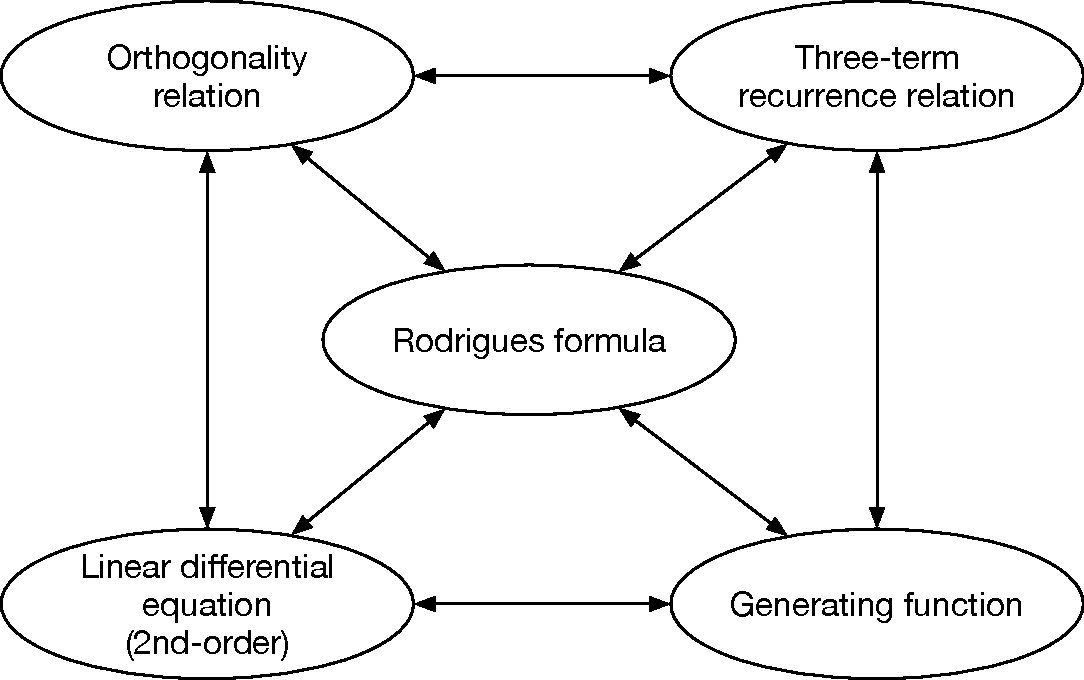
\includegraphics[width=8cm]{./Figures/20170905-poly-types-formulas}
  \label{fig:poly-classical-relations}
%
%  \small{Source: PBOC.}
\end{figure}

\subsection{埃米特多项式}
\label{sec:poly-hermite}
\begin{theorem}[埃米特多项式的罗德里格斯公式]
在区间$(-\infty,+\infty)$内,关于正态分布(normal distribution)\index{normal distribution \dotfill 正态分布} $w(x)=\exp(-x^2)$的埃米特正交多项式(Hermite polynomial)\index{polynomial!Hermite \dotfill{埃米特多项式} } $H_n(x)$,可由罗德里格斯公式予以定义(Rodrigues formula)\index{Rodrigues formula!Hermite polynomial\dotfill 罗德里格斯公式(埃米特多项式)}
\begin{equation}
  \label{eq:poly-hermite-rodrigues-formula}
  H_n(x) = \frac{(-1)^n}{w(x)} D^n w(x) = (-1)^n \exp(x^2) D^n \exp(-x^2), \quad n=0,1,2\ldots
\end{equation}
\end{theorem}
其中$(-1)^n$项是为了保证$\{D^n w(x)\}$的每一个首项系数都为正。$D=\frac{d}{d x}$是微分符,$D^n$是第$n$次求导。$D^n$遵循莱布尼兹法则(Leibniz rule)\index{Leibniz rule \dotfill 莱布尼兹法则}
\begin{equation}
  \label{eq:poly-leibniz-rule}
  D^n \left[f(x) g(x)\right] = \sum_{k=0}^{n} = \sum_{k=0}^{n} \begin{pmatrix} n \\ k \end{pmatrix} D^k f(x) D^{n-k} g(x), \quad n=0,1,2 \ldots,
\end{equation}
其中$\begin{pmatrix} n \\ k \end{pmatrix} = \frac{n!}{(n-k)!}$是帕斯卡三角(Pascal triangle identity)\index{Pascal triangle identity \dotfill 帕斯卡三角}中的二项式系数。帕斯卡三角满足关系
\begin{equation*}
  \begin{pmatrix}
    n+1 \\ k
  \end{pmatrix} = \begin{pmatrix}
    n \\ k
  \end{pmatrix} +
  \begin{pmatrix}
    n \\ k-1
  \end{pmatrix}.
\end{equation*}

帕斯卡三角的简单证明:
\begin{equation*}
\begin{split}
&  \begin{pmatrix}
    n \\ k
  \end{pmatrix} +
  \begin{pmatrix}
    n \\ k-1
  \end{pmatrix} \\
  &= \frac{n!}{k! \, (n-k)!} + \frac{n!}{(k-1)! \, (n-k+1)!}\\
  &=n! \left\{ \frac{n-k+1}{k! (n-k+1)!}  + \frac{k}{k! (n-k+1)!} \right\} \\
  &= \frac{(n+1)!}{k! (n+1-k)!} \\
  &= \begin{pmatrix}
  n+1 \\ k
  \end{pmatrix}.
\end{split}
\end{equation*}

正态分布$w(x)=\exp(-x^2)$在区间$(-3,3)$内,如图\ref{fig:poly-normal-distribution-example}所示。

\begin{figure}[htbp]
   \caption{正态分布}
  \centering
  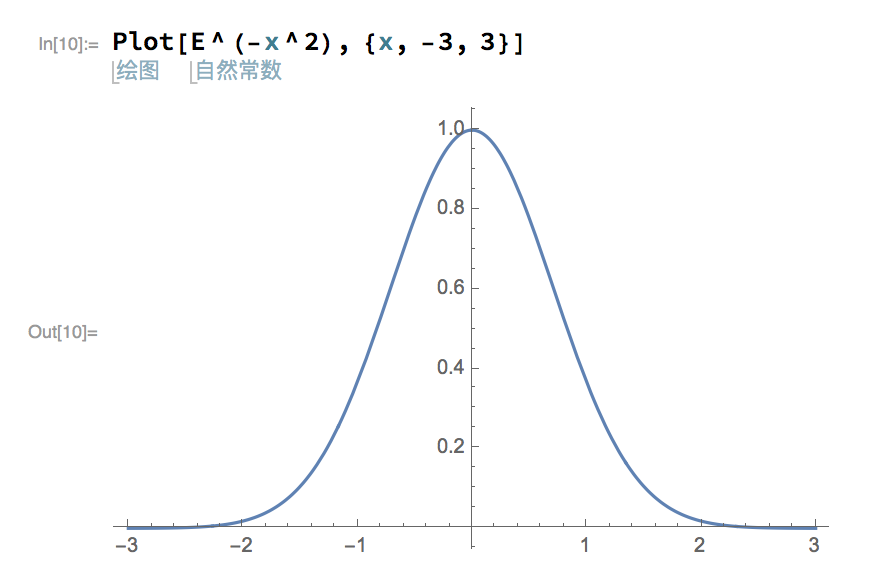
\includegraphics[width=8cm]{./Figures/20170905-normal-distri}
  \label{fig:poly-normal-distribution-example}
%

\small{$w(x) = \exp(-x^2)$在$(-3,3)$区间内的正态分布。}
\end{figure}

\begin{theorem}
  \label{theorem:poly-jacobi-poly-properties}
  由\eqref{eq:poly-hermite-rodrigues-formula}定义的埃米特多项式$H_n(x)$是一个关于$x$的$n$次多项式,并且$H_0(1)=x$,$H_n(x)$的首项系数$k_n=2^n$,$H_{2n}(x)$是偶方程,$H_{2n+1}(x)$是奇方程。
\end{theorem}
\begin{proof}
  \eqref{eq:poly-hermite-rodrigues-formula}$\Rightarrow$
  \begin{equation}
    \label{eq:poly-hermite-dnplus1}
    \begin{split}
      D^{n+1}w(x) &= D \left[D^n w(x) \right] \\
      &= D \left[ (-1)^n H_n(x) w(x) \right] \\
      &= (-1)^n \left[ w'(x) H_n(x) + w(x) H'_n(x) \right] \\
      &= (-1)^n \left[ -2x \exp(-x^2) H_n(x) + w(x) H_n(x) \right] \\
      &= (-1)^{n+1} w(x) \left[ 2x H_n(x) - H'_n(x) \right], \quad n=0,1,2 \ldots
    \end{split}
  \end{equation}

  由此,\eqref{eq:poly-hermite-rodrigues-formula}$\Rightarrow$
  \begin{equation} \label{eq:poly-hermite-diff}
        H_{n+1}(x) = \begin{cases}
        1 & n=0 \\
        \frac{(-1)^{n+1}}{w(x)} D^{n+1} w(x)=2x H_n(x)-H'_n(x) & n=1,2\ldots
        \end{cases}
  \end{equation}
\eqref{eq:poly-hermite-diff}决定了$H_n(x)$是一个$n$次多项式,并且$H_n(x)$的首项系数$k_n=2^n$,可以写出如下序列
\begin{align*}
  &p_0(x) = 1,\\
  &p_1(x) = 2x,\\
  &p_2(x) = 4x^2-2,\\
  &p_3(x) = 8x^3 - 12x,\\
  &p_4(x) = 16 x^4 - 48 x^2 + 12, \\
  &p_5(x) = 32x^5 - 160x^3 + 120x,\\
  &p_6(x) = 64 x^6 - 480 x^4 + 720 x^2 - 120,\\
  &p_7(x) = 128 x^7 - 1344 x^5 + 3360x^3 - 1680x,\\
  &\vdots
\end{align*}
由上式可得,对于偶数次$2n=2,4,6 \ldots$的情况我们有$p_{2n}(x)=p_{2n}(-x)$是偶方程;对于基数次$2n+1=1,3,5 \ldots$的情况我们有$p_{2n+1}(x)=-p_{2n}(-x)$是奇方程,如图\ref{fig:poly-hermite-examples-7-8}。

\begin{figure}[htbp]
   \caption{埃米特多项式}
  \centering
  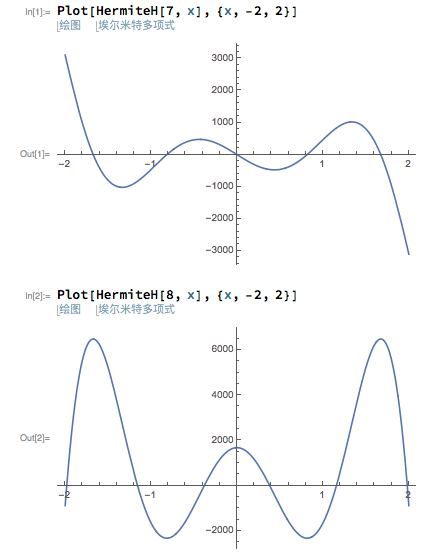
\includegraphics[width=8cm]{./Figures/20170905-hermite-examples-7-8}
  \label{fig:poly-hermite-examples-7-8}
%

\small{上图和下图分别表示$n=7,n=8$时,$H_n(x)$在$(-2,2)$区间内的值。}
\end{figure}
\end{proof}

\begin{theorem}[埃米特多项式的正交条件]
  埃米特多项式$H_n(x)$满足正交条件(orthogonality condition)\index{orthogonality condition!Hermite polynomial \dotfill 正交条件(埃米特多项式)}
  \begin{equation}
    \label{eq:poly-hermite-orthogonality-condition}
    \frac{1}{\sqrt{\pi}} \int_{-\infty}^{\infty} \exp(-x^2) H_m(x) H_n(x) \, dx = 2^n n! \delta_{mn}, \quad m,n = 0,1,2\ldots
  \end{equation}
\end{theorem}

\begin{proof}
由埃米特多项式的罗德里格斯定义式\eqref{eq:poly-hermite-rodrigues-formula}我们有,当$m<n$时
\begin{equation*}
  \begin{split}
    \int_{-\infty}^{\infty} \exp(-x^2) H_m(x) H_n(x) \, dx &= \int_{-\infty}^{\infty} \exp(-x^2) H_m(x) \left[ (-1)^n \exp(x^2) D^n \exp(-x^2) \right] \, dx \\
    &= \int_{-\infty}^{\infty} (-1)^n \exp(-x^2) H_m(x) \, dx,  \end{split}
\end{equation*}
对上式做$n$次求导,积分内的值变为零。

当$m=n$时$\Rightarrow$
\begin{equation*}
  \begin{split}
    \frac{1}{\sqrt{\pi}}  \int_{-\infty}^{\infty} \exp(-x^2) H_m(x) H_n(x) \, dx &= \frac{1}{\sqrt{\pi}} \int_{-\infty}^{\infty} \exp{(-x^2)} H_n(x) H_n(x) \, dx\\
    &=\frac{1}{\sqrt{\pi}} (-1)^n \int_{-\infty}^{\infty}  H_n(x) D^n \exp(-x^2) \, dx\\
    &=\frac{1}{\sqrt{\pi}} \int_{-\infty}^{\infty}  D^n H_n(x)  \exp(-x^2) \, dx\\
    &=\frac{k_n n!}{\sqrt{\pi}} \int_{-\infty}^{\infty} \exp (-x^2) \, dx \\
    &= k_n n!.
  \end{split}
\end{equation*}
证毕。
\end{proof}

\begin{theorem}[埃米特多项式的三项递推关系]
  埃米特多项式的三项递推关系\index{three-term recurrence relation!Hermite polynomial \dotfill 三项递推关系(埃米特多项式)}为
  \begin{equation}
    \label{poly-hermite-three-term-recurrence-relation}
    H_{n+1}(x) = 2x H_n(x) - 2n H_{n-1}(x), n=1,2,3\ldots
  \end{equation}
\end{theorem}
\begin{proof}
由正态分布$w(x)=\exp(-x^2)$我们有
\begin{equation*}
  w'(x) = -2x w(x).
\end{equation*}

代入莱布尼兹法则\eqref{eq:poly-leibniz-rule}$\Rightarrow$
\begin{equation*}
  \begin{split}
    D^{n+1}w(x) = D^n w'(x) =D^n \left[ -2x w(x) \right] = (-2x) D^n w(x) + (-2n) D^{n-1} w(x).
  \end{split}
\end{equation*}

将上式代回\eqref{eq:poly-hermite-diff}$\Rightarrow$
\begin{equation*}
  \begin{split}
    H_{n+1}(x) &= \frac{(-1)^{n+1}}{w(x)} D^{n+1}w(x)\\ %= \left[ 2xH_n(x) - H'_n(x) \right]\\
    &= (-1) \frac{(-1)^n}{w(x)} (-2x) D^n w(x) + (-1)^2  \frac{(-1)^{n-1}}{w(x)} (-2n) D^{n-1}w(x) \\
    &= \frac{(-1)^{n}}{w(x)} w(x) D^n w(x) - 2n \frac{(-1)^{n-1}}{w(x)}D^{n-1}w(x)\\
    &=2x H_n(x) - 2n H_{n-1}(x), n=1,2,3\ldots
  \end{split}
\end{equation*}
\end{proof}

\begin{theorem}[埃米特多项式的二阶线性微分方程]
  埃米特多项式的二阶线性微分方程(second order linear differential equation)\index{second order linear differential equation!Hermite polynomial \dotfill 二阶线性微分方程(埃米特多项式)}为
  \begin{equation}
    \label{eq:poly-hermite-differential-equation}
    H''_n(x) + 2n H_n(x) - 2x H'_n(x)=0.
  \end{equation}
\end{theorem}
\begin{proof}
  联立埃米特多项式的罗德里格斯公式\eqref{eq:poly-hermite-rodrigues-formula}和三项递归关系式\eqref{poly-hermite-three-term-recurrence-relation}我们有
  \begin{equation*}
  \begin{split}
    H'_n(x) = 2n H_{n-1}(x), n=1,2,3 \ldots \\
    H'_{n+1}(x) = 2(n+1) H_{n}(x), n=0,1,2 \ldots
  \end{split}
\end{equation*}

  对\eqref{eq:poly-hermite-diff}再做一次求导,并引入上式替换$H'_{n+1}(x)$我们有
  \begin{align*}
    &H'_{n+1}(x) = 2x H'_n(x) + 2 H_n(x) - H''_n(x), \\
    &\hookrightarrow 2(n+1) H_n(x) = 2x H'_n(x) + 2H_n(x) - H''(x),
  \end{align*}
这意味着$H_n(x)$构成一个二阶线性微分方程系统
\begin{equation}
  \label{eq:poly-hermite-diff-eq}
  y''(x) - 2xy'(x) + 2n y(x)=0.
\end{equation}
\end{proof}

\begin{theorem}[埃米特多项式的母方程]
  埃米特多项式的母方程(generating function)\index{generating function!Hermite polynomial \dotfill 母方程(埃米特多项式)}为
  \begin{equation}
    \label{eq:poly-hermite-generating-function}
    \exp(2xt-t^2) = \sum_{n=0}^{\infty}  \frac{H_n(x)}{n!} t^n.
  \end{equation}
\end{theorem}

\begin{proof}
  设$F(t) = \exp(-(x-t)^2) = \exp(-x^2) \exp(2xt-t^2)$. 围绕$\tilde{t}=0$对$F(t)$做泰勒级数展开近似
  \begin{equation*}
    F(t) \approx \sum_{n}^{\infty} \frac{F^{n}(0)}{n!} t^n.
  \end{equation*}

  设$u=x-t$,$\lim_{t \rightarrow 0} u \approx x$。则
  \begin{equation*}
    \begin{split}
      F^{n}(0) &= \frac{d^n}{d t^n} \exp(-(x-t)^2) = \left[ (-1)^n \frac{d^n}{d u^n} \exp(-u^2) \right]_{u=x} \\
      &=(-1)^n D^n \exp(-x^2) = \exp(-x^2) H_n(x), n=0,1,2\ldots
    \end{split}
  \end{equation*}

  $\hookrightarrow$
  \begin{equation*}
    \begin{split}
      &\exp(-x^2) \exp(-2xt-t^2) = \exp(-(x-t)^2) \\
      &= F(t) = \sum_{n=0}^{\infty} \frac{f^{(n)}(0)}{n!} t^n = \exp(-x^2) \sum_{t=0}^{\infty} \frac{H_n(x)}{n!} t^n.
    \end{split}
  \end{equation*}
\end{proof}

\subsection{拉盖尔多项式}
\label{sec:poly-laguerre}
\begin{theorem}[拉盖尔多项式的罗德里格斯公式]
在$(0,\infty)$区间内,关于伽玛分布(Gamma distribution)\index{gamma distribution \dotfill 伽玛分布} $w(x) = \exp(-x) x^{\alpha}$的拉盖尔多项式(Laguerre polynomial)\index{polynomial!Laguerre \dotfill 拉盖尔多项式} $L^{(\alpha)}_n(x)$,可由罗德里格斯公式予以定义\index{Rodrigues formula!Laguerre polynomial\dotfill 罗德里格斯公式(拉盖尔多项式)}

\begin{equation}
  \label{eq:poly-laguerre-rodrigues-formula}
  L^{(\alpha)}_n(x) = \frac{1}{n!} \frac{1}{w(x)} D^n \left[ w(x)x^n \right]= \frac{1}{n!} \exp(x) x^{-\alpha} D^n \left[ \exp(-x) x^{n+\alpha} \right], \quad n=0,1,2\ldots
\end{equation}
\end{theorem}
当$\alpha=1/2$时伽玛分布$w(x) = \exp (-x) x^{\alpha}$在区间$(-3,3)$内,如图\ref{fig:poly-gamma-distribution-example}所示。

\begin{figure}[htbp]
   \caption{伽玛分布}
  \centering
  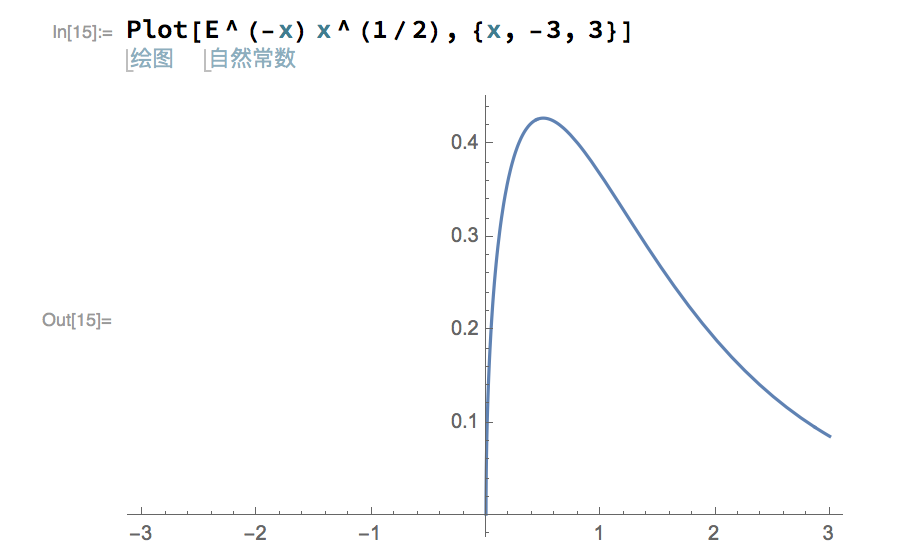
\includegraphics[width=8cm]{./Figures/20170906-gamma-distri}
  \label{fig:poly-gamma-distribution-example}
%

\small{$w(x) = \exp(-x) x^{\alpha}$在$(-3,3)$区间内的正态分布$(\alpha = 1/2)$。}
\end{figure}

\begin{theorem}
  拉盖尔多项式$L^{(n)}(x)$是一个关于$x$的$n$次多项式。$L^{(\alpha)}(0) = \frac{(\alpha+1)_n}{n!}$,$L^{(n)}(x)$的首项系数$k_n = \frac{(-1)^n}{n!}$。
\end{theorem}
\begin{proof}
  根据莱布尼兹法则\eqref{eq:poly-leibniz-rule}我们有
  \begin{equation*}
    \begin{split}
      D^n \left[ \exp(-x) x^{n+\alpha} \right] &= \sum_{k=0}^n \begin{pmatrix} n \\ k \end{pmatrix} D^k \exp(-x) D^{n-k} x^{n+\alpha} \\
      &= \sum_{k=0}^{n} \begin{pmatrix} n \\ k \end{pmatrix} (-1)^k \exp(-x) x^{\alpha + k }(n+\alpha)(n+\alpha-1) \ldots (n + k + 1) \\
      &= \exp(-x) x^{\alpha}  \sum_{k=0}^{n} (-1)^k \begin{pmatrix} n \\ k \end{pmatrix} \frac{\Gamma (n+\alpha + 1)}{\Gamma (k + \alpha + 1)} x^k.
    \end{split}
  \end{equation*}
最后一个等式的简单数学计算:
\begin{equation*}
  \begin{split}
    \frac{\Gamma (n+\alpha + 1)}{\Gamma (k + \alpha + 1)} &= \frac{
    \int_0^{\infty} \exp(-t) t^{n+\alpha} \, dt
    }{
    \int_0^{\infty} \exp(-t) t^{k+\alpha} \, dt
    } \approx \frac{(n+\alpha)!}{(k+\alpha)!}
  \end{split}
\end{equation*}

因此我们有
\begin{equation}
  \label{eq:poly-laguerre-def-intermediate}
  L_n^{(\alpha)}(x) = \sum_{k=0}^n (-1)^k \begin{pmatrix} n+\alpha \\ n-k \end{pmatrix} \frac{x^k}{k!}, \quad \text{其中} \begin{pmatrix} n+\alpha \\ n-k \end{pmatrix} = \frac{\Gamma (n+\alpha + 1)}{\Gamma (k + \alpha + 1)}(n-k)!
\end{equation}
由上式可见,$L^{(\alpha)}_n(x)$是一个$n$次多项式。此外,由于
\begin{equation*}
  (-1)^k \begin{pmatrix} n+\alpha \\ n-k \end{pmatrix} = \frac{(-1)^k}{(n-k)!}\frac{(n+\alpha)!}{(\alpha + k)!} = \frac{(-1)^k}{(n-k)!} \frac{(\alpha +1)_n}{(\alpha+1)_k} = \frac{(\alpha+1)_n}{n!} \frac{(-n)_k}{(\alpha+1)_k},
\end{equation*}
我们可得拉盖尔多项式的超几何方程\index{hypergeometric function!Laguerre polynomial \dotfill 超几何方程(拉盖尔多项式)}
\begin{equation}
  \label{eq:poly-laguerre-hgf}
  L_n^{(\alpha)}(x) = \frac{(\alpha+1)_n}{n!} \sum_{k=0}^{n} \frac{(-n)_k}{(\alpha+1)_k} \frac{x^k}{k!} = \begin{pmatrix}
  n+\alpha \\ n
\end{pmatrix}\pFq{1}{1}{-n}{\alpha+1}{x}.
\end{equation}

由\eqref{eq:poly-laguerre-hgf}得$x=0$时
\begin{equation*}
  L^{(\alpha)}_n(0) = \begin{pmatrix} n+\alpha \\ n \end{pmatrix} = \frac{(\alpha+1)_n}{n!}, \quad n=0,1,2\ldots
\end{equation*}
$\hookrightarrow$
\begin{equation*}
  k_n = \frac{(-1)^n}{n!}, \quad n=0,1,2\ldots
\end{equation*}
\end{proof}

\begin{theorem}[拉盖尔多项式的正交条件]
  拉盖尔多项式$L^{(\alpha)}_n(x)$的正交条件\index{orthogonality condition!Laguerre polynomial \dotfill 正交条件(拉盖尔多项式)}满足
  \begin{equation}
    \label{eq:poly-laguerre-poly-orghogonality-condition}
    \int_0^{\infty} \exp(-x) x^{\alpha} L_m^{(\alpha)}(x) L_n^{(\alpha)}(x) \, dx = \frac{\Gamma(n+\alpha+1)}{n!} \delta_{mn}, \alpha > -1.
  \end{equation}
\end{theorem}
\begin{proof}
  定义矩
\begin{equation*}
  \mu_n := \int_0^{n} \exp(-x) x^{n+\alpha} \, dx,
\end{equation*}
如果对于所有$n=0,1,2\ldots$,$\mu_n$都存在,那么\eqref{eq:poly-laguerre-poly-orghogonality-condition}的LHS积分是收敛的,因此需要$\alpha > -1$\todo{这部分还需要做进一步的说明。}。此外根据定义我们有
\begin{equation*}
  \mu_n = \Gamma (n+\alpha + 1).
\end{equation*}

进而,由拉盖尔多项式的罗德里格斯公式\eqref{eq:poly-laguerre-rodrigues-formula}我们有

\begin{equation*}
  \begin{split}
    &\int_0^{\infty} \exp(-x) x^{\alpha} L_m^{(\alpha)}(x) L_n^{(\alpha)}(x) \, dx
    \\&= \int_0^{\infty} \exp(-x) x^{\alpha} L_m^{(\alpha)}(x) \left\{
    \frac{1}{n!} \exp(-x) x^{\alpha} D^n \left[ \exp(-x) x^{n+\alpha} \right]
    \right\} \, dx \\
    &= \frac{-1}{n!} \int_0^{\infty} L_m^{(\alpha)} (x) D^n \left[ \exp(-x) x^{n+\alpha}  \right] \, dx \\
    &= \frac{(-1)^n}{n!} \int_0^{\infty} L_m^{(\alpha)} (x) D^n \left[ \exp(-x) x^{n+\alpha}  \right] \, dx
  \end{split}
\end{equation*}
当$m<n$时,对上式做$n$次求导,积分内的值变为零。当$m=n$时 $\Rightarrow$
\begin{equation*}
  \begin{split}
    &\frac{(-1)^n}{n!} \int_0^{\infty} L_m^{(\alpha)} (x) D^n \left[ \exp(-x) x^{n+\alpha}  \right] \, dx \\
    &= \frac{(-1)^n}{n!} k_n n! \int_0^{\infty} \exp(-x) x^{n+\alpha} \, dx \\
    &= \frac{\Gamma (n+\alpha + 1)}{n!}.
  \end{split}
\end{equation*}
\end{proof}

\begin{theorem}[拉盖尔多项式的母方程]
  拉盖尔多项式$L_n^{(\alpha)}(x)$的母方程\index{generating function!Laguerre polynomial \dotfill 母方程(拉盖尔多项式)}为
  \begin{equation}
    \label{eq:poly-laguerre-generating-function-def}
    (1-t)^{-\alpha - 1} \exp \left( - x \frac{t}{1-t} \right) = \sum_{n=0}^{\infty} L_n^{(\alpha)}(x) t^n.
  \end{equation}
\end{theorem}
\begin{proof}
将\eqref{eq:poly-laguerre-hgf}代入\eqref{eq:poly-laguerre-generating-function-def}RHS $\Rightarrow$
\begin{equation*}
  \begin{split}
    &\sum_{n=0}^{\infty} L_n^{(\alpha)}(x) t^n \\
    &=\sum_{n=0}^{\infty} \frac{(\alpha+1)_n}{n!} t^n \sum_{k=0}^{n} \frac{
    (-n)_k
    }{
    (\alpha + 1)_k
    } \frac{
    x^k
    }{k!}\\
    &=\sum_{k=0}^{\infty} \sum_{n=0}^{\infty} \frac{(\alpha+1)_n}{(\alpha+1)_k} \frac{
    (-1)^k x^k t^n
    }{
    k! (n-k)!
    } \\
    &=\sum_{k=0}^{\infty} \sum_{n=0}^{\infty}
    \frac{(\alpha+1)_{n+k}}{(\alpha+1)_k}
    \frac{(-1)^k x^k t^{n+k}}{k! n!}\\
    &= \sum_{k=0}^{\infty} \frac{(- x t)^k}{k!}
    \sum_{n=0}^{\infty} \frac{(\alpha + k + 1)_n}{n!} t^n \\
    &=\sum_{k=0}^{\infty} \frac{(-xt)^k}{k!} (1-t)^{(-\alpha - k - 1)}\\
    &=(1-t)^{-\alpha -1} \sum_{k=0}^{\infty} \frac{1}{k!} \left(- x \frac{t}{1-t} \right)^{k}\\
    &=(1-t)^{-\alpha - 1} \exp \left( - x \frac{t}{1-t} \right).
  \end{split}
\end{equation*}
\end{proof}

\begin{theorem}
  由拉盖尔多项式的母方程\eqref{eq:poly-laguerre-generating-function-def}我们有
  \begin{equation}
    L_n^{(\alpha + \beta + 1)}(x + y) = \sum_{k=0}^{n} L_{k}^{(\alpha)} (x) L_{n-k}^{(\beta)} (y).
  \end{equation}
\end{theorem}
\begin{proof}
  \eqref{eq:poly-laguerre-generating-function-def}$\Rightarrow$
  \begin{equation*}
    \begin{split}
    \sum_{n=0}^{\infty}  L_n^{(\alpha + \beta + 1)} (x + y) t^n &= (1-t)^{- \alpha - \beta -2} \exp \left[ - (x+y)\frac{t}{1-t}\right] \\
    &= \left[ (1-t)^{-\alpha -1} \exp \left( -x \frac{t}{1-t} \right) \right] \left[ (1-t)^{(-\beta - 1)} \exp \left(-y \frac{1}{1-t} \right) \right]\\
    &=\left[ \sum_{k=0}^{\infty} L_{k}^{(\alpha)} (x) t^k \right] \left[ \sum_{m=0}^{\infty} L_{m}^{(\beta)} (y) t^m\right] \\
    &=\sum_{n=0}^{\infty} \left[ \sum_{k=0}^{n} L_{k}^{(\alpha)}(x) L_{n-k}^{(\beta)}(y) \right] t^n.
    \end{split}
  \end{equation*}
  证毕。
\end{proof}

\begin{theorem}[拉盖尔多项式的三项递推关系]
  拉盖尔多项式$L_n^{(\alpha)}(x)$的三项递推关系\index{three-term recurrence relation!Laguerre polynomial \dotfill 三项递推关系(拉盖尔多项式)}为
  \begin{equation}
    \label{eq:poly-laguerre-three-term-recurrence-relation}
    (n+1) L_{n+1}^{(\alpha)}(x) + (x - 2n - \alpha - 1) L_{n}^{(\alpha)}(x) + (n+\alpha) L_{n-1}^{(\alpha)}(x) =0, \quad n = 1,2,3\ldots
  \end{equation}
\end{theorem}

\begin{proof}

首先由\eqref{eq:poly-laguerre-def-intermediate}得
\begin{equation}
  \label{eq:poly-laguerre-diff-x}
\begin{split}
    \frac{d}{dx} L_n^{(\alpha)}(x) &= \frac{d}{dx} \sum_{k=0}^{n} (-1)^k \begin{pmatrix}
    n+\alpha \\ n-k
  \end{pmatrix} \frac{x^k}{k!}\\
  &=\sum_{k=1}^{n} (-1)^k \begin{pmatrix}
  n+\alpha \\ n-k
\end{pmatrix}  \frac{x^{k-1}}{(k-1)!} \\
&= \sum_{k=0}^{n-1} (-1)^{k-1} \begin{pmatrix}
n+\alpha \\ n-k-1
\end{pmatrix}  \frac{x^{k}}{(k)!}\\
&= - L_{n-1}^{(\alpha + 1)}(x), n=1,2,3\ldots
\end{split}
\end{equation}
为简化表述,根据拉盖尔多项式的母方程\eqref{eq:poly-laguerre-generating-function-def},定义
\begin{equation*}
  F(x,t) := (1-t)^{-\alpha - 1} \exp \left( - x \frac{t}{1-t} \right) = \sum_{n=0}^{\infty} L_n^{(\alpha)}(x) t^n.
\end{equation*}

则我们有第一个偏导数
\begin{equation}
  \label{eq:poly-laguerre-three-partial-f-x}
  \begin{split}
    &\frac{\partial F(x,t)}{\partial x} = (-t) (1-t)^{-\alpha - 2} \exp \left( - x \frac{t}{1-t} \right), \\
    &\Rightarrow (1-t) \frac{\partial F(x,t)}{\partial x} + t F(x,t) = 0,\\
    &\Rightarrow (1-t) \sum_{n=0}^{\infty} \frac{d}{dx} L_n^{(\alpha)}(x) t^n + t \sum_{n=0}^{\infty} L_n^{(\alpha)} (x) t^n = 0, \\
    & \Rightarrow \underbrace{\sum_{n=0}^{\infty} \frac{d}{dx} L_n^{(\alpha)}(x) t^n}_{n\rightarrow n+1} - \sum_{n=0}^{\infty} \frac{d}{dx} L_n^{(\alpha)}(x) t^{n+1} + \sum_{n=0}^{\infty} L_n^{(\alpha)} (x) t^n = 0,\\
    & \Rightarrow \frac{d}{dx} L_{n+1}^{(\alpha)}(x)
    - \frac{d}{dx} L_n^{(\alpha)}(x)
    + L_n^{(\alpha)} (x)= 0,
  \end{split}
\end{equation}

上式代入\eqref{eq:poly-laguerre-diff-x}有
\begin{equation*}
\begin{split}
  &-L_n^{(\alpha+1)}(x) - \frac{d}{dx}L_n^{(\alpha)}(x) + L_n^{(\alpha)}(x)=0, \\
  &\Rightarrow \frac{d}{dx}L_n^{(\alpha)}(x) = L_n^{(\alpha)}(x) - L_n^{(\alpha+1)}(x), \quad n = 0,1,2\ldots
\end{split}
\end{equation*}

第二个偏导数
\begin{equation*}
\begin{split}
  &\frac{\partial F(x,t)}{\partial t} =
  \left[ (\alpha + 1) (1-t)^{-\alpha - 2} + (1-t)^{-\alpha - 1} \frac{-x(1-t)-xt}{(1-t)^2} \right] \exp \left( - x \frac{t}{1-t} \right) \\
  &=\left(\alpha + 1 - \frac{x}{1-t} \right) (1-t)^{-\alpha - 2} \exp \left( - x \frac{t}{1-t} \right), \\
  &\Rightarrow (1-t)^2 \frac{\partial F(x,t)}{\partial t} + \left[ x - (\alpha - 1)(1-t) \right] F(x,t) = 0,\\
  &\Rightarrow (1-t)^2 \sum_{n=1} n L_n^{(\alpha)} (x) t^{(n-1)} + \left[ x - (\alpha + 1) (1-t) \right] \sum_{n=0}^{\infty} L_n^{\alpha} (x) t^n = 0,
  \end{split}
\end{equation*}
将各项拆出
\begin{equation*}
  \begin{split}
    &\sum_{n=1}^{\infty} n L_{n}^{\alpha}(x) t^{n-1}
    -2 \sum_{n=1}^{\infty} n L_{n}^{\alpha}(x) t^n
    + \sum_{n=1}^{\infty} n L_{n}^{\alpha}(x) t^{n+1} \\
    &+ x \sum_{n=0}^{\infty} L_{n}^{\alpha}(x) t^n
    + (\alpha + 1) \sum_{n=0}^{\infty} L_{n}^{\alpha}(x) t^{n+1}
    -(\alpha+1) \sum_{n=0}^{\infty} L_{n}^{\alpha}(x) t^n = 0,
  \end{split}
\end{equation*}

按照$t$的幂次重新排列组合,得三项递推关系式\eqref{eq:poly-laguerre-three-term-recurrence-relation}。
\end{proof}

\begin{theorem}[拉盖尔多项式的二阶线性微分方程]
  拉盖尔多项式$L_n^{(\alpha)}(x)$的二阶线性微分方程\index{second order linear differential equation!Laguerre polynomial \dotfill 二阶线性微分方程(拉盖尔多项式)}为
  \begin{equation*}
    \label{eq:poly-laguerre-linear-diff-equation}
    x \frac{d^2}{d x^2}L_n^{(\alpha)}(x)+ \left( \alpha + 1 - x \right) \frac{d}{dx}L_n^{(\alpha)}(x) + n  L_n^{(\alpha)}(x) = 0.
  \end{equation*}
\end{theorem}
\begin{proof}
  拉盖尔多项式的三项递推关系\eqref{eq:poly-laguerre-three-term-recurrence-relation}$\Rightarrow$
  \begin{equation*}
    x L_n^{(\alpha)}(x) + (n+1) \left[ L_{n+1}^{(\alpha)}(x) - L_n^{(\alpha)}(x)\right] - (n + \alpha)  \left[ \frac{d}{dx}L_n^{(\alpha)}(x) -  \frac{d}{dx}L_{n-1}^{(\alpha)}(x) \right]=0.
  \end{equation*}

对$x$求导$\Rightarrow$
\begin{equation*}
  \begin{split}
    L_n^{(\alpha)} (x) + x \frac{d}{dx} L_n^{(\alpha)} (x) + (n+1) \frac{d}{dx} L_{n+1}^{(\alpha)} (x) - (n+1) \frac{d}{dx} L_{n}^{(\alpha)} (x) - (n+\alpha) \frac{d}{dx} L_{n}^{(\alpha)} (x) + (n+\alpha) \frac{d}{dx} L_{n-1}^{(\alpha)} (x) = 0,
  \end{split}
\end{equation*}
引入\eqref{eq:poly-laguerre-three-partial-f-x}替换上式中的$\frac{d}{dx}L_{n+1}^{(\alpha)}(x)$和$\frac{d}{dx}L_{n}^{(\alpha)}(x)$
  \begin{align}
    &L_n^{(\alpha)} (x)+ x \frac{d}{dx} L_n^{(\alpha)} (x) - (n+1) L_n^{(\alpha)} (x) + (n+\alpha) L_{n-1}^{(\alpha)} (x) = 0, \nonumber \\
    \label{eq:poly-laguerre-first-order-diff}
    &x \frac{d}{dx} L_n^{(\alpha)} (x) = n L_n^{(\alpha)} (x) - (n+\alpha) L_{n-1}^{(\alpha)} (x).
  \end{align}
  上式继续对$x$求导$\Rightarrow$
  \begin{equation}
    \label{eq:poly-laguerre-second-order-diff}
      \begin{split}
        \frac{d}{dx} L_n^{(\alpha)} (x) + x \frac{d^2}{dx^2} L_n^{(\alpha)} (x) &= n \frac{d}{dx} L_n^{(\alpha)} (x) -(n+\alpha) \frac{d}{dx} L_{n-1}^{(\alpha)} (x) \\
        &= (n+\alpha) \left( \frac{d}{dx} L_n^{(\alpha)} (x)- \frac{d}{dx} L_{n-1}^{(\alpha)} (x) \right) - \alpha \frac{d}{dx} L_n^{(\alpha)} (x) \\
        &= -(n+\alpha) L_{n-1}^{(\alpha)} (x) - \alpha \frac{d}{dx} L_n^{(\alpha)} (x) \\
        &= x \frac{d}{dx}L_n^{(\alpha)} (x) - n L_n^{(\alpha)} (x) - \alpha \frac{d}{dx}L_n^{(\alpha)} (x),
      \end{split}
  \end{equation}
  $\hookrightarrow$
  \begin{equation*}
    \begin{split}
      \frac{d^2}{dx^2} L_n^{(\alpha)}(x) + (1 + \alpha - x) \frac{d}{dx} L_n^{(\alpha)}(x) + n L_n^{(\alpha)}(x) = 0, \\
      \Rightarrow xy''(x) + (1 + \alpha - x) y'(x) + n y(x) =0, \quad n=0,1,2\ldots
    \end{split}
  \end{equation*}
\end{proof}

\subsection{雅各比多项式}
\label{sec:poly-jacobi-polynomial}
\begin{theorem}[雅各比多项式的罗德里格斯公式]
在$(-1,1)$区间内,关于贝塔分布(Beta distribution)\index{Beta distribution \dotfill 贝塔分布} $w(x)=(1-x)^{\alpha} (1+x)^{\beta}$的雅各比多项式(Jacobi polynomial)\index{polynomial!Jacobi \dotfill 雅各比多项式} $P_n^{(\alpha,\beta)}(x)$ ,可由罗德里格斯公式\index{Rodrigues formula!Jacoby polynomial \dotfill 罗德里格斯公式(雅各比多项式)}予以定义
\begin{equation}
  \label{eq:poly-jacobi-polynomial-def}
  \begin{split}
    P_n^{(\alpha,\beta)} (x) &= \frac{(-1)^n}{2^n n!} \frac{1}{w(x)} D^n \left[ w(x) (1-x^2)^n \right] \\
    &= \frac{(-1)^n}{2^n n!} (1-x)^{-\alpha} (1+x)^{-\beta} D^n \left[ (1-x)^{n+\alpha} (1+x)^{n+\beta} \right], \quad \alpha, \beta > -1, n=0,1,2\ldots
  \end{split}
\end{equation}
\end{theorem}

当$(\alpha,\beta)=(3,2)$时贝塔分布$w(x)=(1-x)^{\alpha} (1+x)^{\beta}$在区间$(-2,2)$内,如图\ref{fig:poly-beta-distribution-example}所示。

\begin{figure}[htbp]
   \caption{贝塔分布}
  \centering
  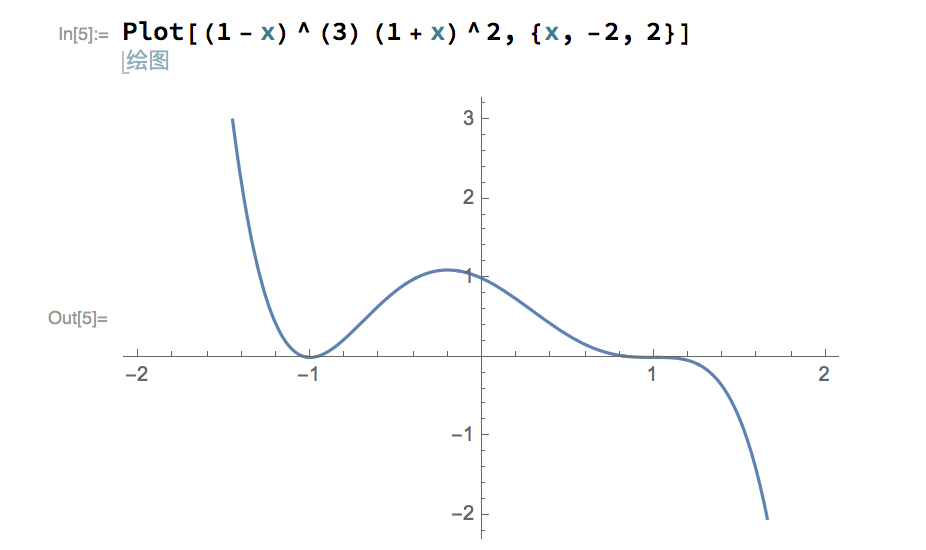
\includegraphics[width=8cm]{./Figures/20170906-beta-distri}
  \label{fig:poly-beta-distribution-example}
%

\small{$w(x)=(1-x)^{\alpha} (1+x)^{\beta}$在$(-2,2)$区间内的正态分布$(\alpha = 3, \beta = 2)$。}
\end{figure}

\begin{theorem}
  \label{theorem:poly-jacobi-properties}
  雅各比多项式$P_n^{(\alpha,\beta)}(x)$是一个关于$x$的$n$次多项式。$P_n^{(\alpha,\beta)}(x)$是奇方程,并且$P_n^{(\alpha,\beta)}(1) = \begin{pmatrix} n+\alpha \\ n \end{pmatrix}$, $P_n^{(\alpha,\beta)}(-1) = (-1)^n \begin{pmatrix} n+\beta \\ n \end{pmatrix}, \quad n=0,1,2\ldots$
\end{theorem}
\begin{proof}
  根据莱布尼兹法则\eqref{eq:poly-leibniz-rule}我们有
  \begin{equation*}
    \begin{split}
      &D^n \left[  (1-x)^{n+\alpha} (1+x)^{n+\beta} \right] \\
      &= \sum_{k=0}^{n} \begin{pmatrix}
      n \\ k
      \end{pmatrix}
      D^k (1-x)^{n+\alpha} D^{n-k} (1+x)^{n+\beta} \\
      &=\sum_{k=0}^{n} \begin{pmatrix}
      n \\ k
      \end{pmatrix} (-1)^k
      (n+\alpha) (n+\alpha-1) (n+\alpha-2) \ldots (n+\alpha-k+1) (1-x)^{n+\alpha-k} \\
      &\qquad \times  (n+\beta) (n+\beta-1) (n+\beta-2) \ldots (\beta+k+1) (1+x)^{\beta+k} \\
      &=n! \sum_{k=0}^{n} (-1)^k \begin{pmatrix}
      n+\alpha \\ k
      \end{pmatrix}
      \begin{pmatrix}
        n+\beta \\ n-k
      \end{pmatrix}
      (1-x)^{n+\alpha - k} (1+x)^{\beta + k}, \quad n=0,1,2\ldots
    \end{split}
  \end{equation*}

代回\eqref{eq:poly-jacobi-polynomial-def}$\Rightarrow$
\begin{equation}
  \label{eq:poly-jacobi-poly-degree-n}
  \begin{split}
    P_n^{(\alpha,\beta)} (x) &= \frac{(-1)^n}{2^n n!} (1-x)^{-\alpha} (1+x)^{-\beta} D^n \left[ (1-x)^{n+\alpha} (1+x)^{n+\beta} \right] \\
    &= \frac{(-1)^n}{2^n} \sum_{k=0}^{n} (-1)^k \begin{pmatrix}
    n+\alpha \\ k
    \end{pmatrix}
    \begin{pmatrix}
      n+\beta \\ n-k
    \end{pmatrix}
    (1-x)^{n- k} (1+x)^k, \quad n=0,1,2\ldots
  \end{split}
\end{equation}

这表明雅各比多项式$P_n^{(\alpha,\beta)}(x)$是一个关于$x$的$n$次多项式。

\eqref{eq:poly-jacobi-polynomial-def} $\Rightarrow$ $P_n^{(\alpha,\beta)}(x)$的对称性(略):
\begin{equation}
  \label{eq:poly-jacobi-symmetry}
  P_n^{(\alpha,\beta)}(-x) = (-1)^n P_n^{(\alpha,\beta)}(x), \quad n=0,1,2 \ldots
\end{equation}

\eqref{eq:poly-jacobi-polynomial-def} $\Rightarrow$
\begin{align*}
  &P_n^{(\alpha,\beta)}(1) = \frac{(-1)^n}{2^n} \sum_{k=0}^{n} (-1)^k \frac{(n+\alpha)!}{(n+\alpha-k)! \, k!}\frac{(n+\beta)!}{(n+\beta+k)! \, (n-k)!} (1+x)^k = \begin{pmatrix}
  n+\alpha \\ n
  \end{pmatrix},\\
  & P_n^{(\alpha,\beta)}(-1) = (-1)^n \begin{pmatrix}
  n+\beta \\ n
  \end{pmatrix}.
\end{align*}
\end{proof}

\begin{theorem}[雅各比多项式的超几何方程]
  \label{theorem:poly-jacobi-hgf}
雅各比多项式的$P_n^{(\alpha,\beta)}(x)$的超几何方程\index{hypergeometric function!Jacobi polynomial \dotfill 超几何方程(雅各比多项式)}可表示为
\begin{equation}
  \label{eq:poly-jacobi-hypergeometric-function}
  P_{n}^{(\alpha, \beta)}(x) = \begin{pmatrix}
  n+\alpha \\ n
  \end{pmatrix}
  \pFq{2}{1}{-n,n+\alpha+\beta+1}{\alpha+1}{\frac{1-x}{2}}, \quad n=0,1,2\ldots
\end{equation}
\end{theorem}
\begin{proof}
  对于$x \neq 1$的情况,  \eqref{eq:poly-jacobi-poly-degree-n}$\Rightarrow$
  \begin{equation*}
    P_n^{(\alpha,\beta)}(x) = \left(\frac{x-1}{2}\right)^n \sum_{k=0}^{\infty} \begin{pmatrix}
    n+\alpha \\ n
    \end{pmatrix}
    \begin{pmatrix}
      n+\beta \\ n-k
    \end{pmatrix}
    \underbrace{\left( \frac{x+1}{x-1} \right)^k}, \quad n=0,1,2\ldots
  \end{equation*}
其中
\begin{equation}
  \label{eq:poly-jacobi-hgf-intermediate}
  \begin{split}
    \left( \frac{x+1}{x-1} \right)^k &= \left( 1 + \frac{2}{x-1} \right)^k, \quad k=0,1,2 \ldots \\
    &= \sum_{i=0}^{k} \begin{pmatrix}
    k \\ i
    \end{pmatrix}
    \left( \frac{2}{x-1} \right)^i \\
    &=  \left( \frac{2}{x-1} \right)^{n} \sum_{i=0}^{n} \sum_{k=i}^{n}
    \begin{pmatrix}
    n+\alpha \\ k
    \end{pmatrix}
    \begin{pmatrix}
    n+\beta \\ n-k
    \end{pmatrix}
    \begin{pmatrix}
    k \\ i
    \end{pmatrix}
     \left( \frac{2}{x-1} \right)^{i} \\
     &= \left( \frac{2}{x-1} \right)^{n} \sum_{i=0}^{n}\sum_{k=0}^{n-i}
     \begin{pmatrix}
      n+ \alpha \\ i+k
     \end{pmatrix}
     \begin{pmatrix}
      n+ \beta \\ n-i-k
     \end{pmatrix}
     \begin{pmatrix}
      i+k \\ k
     \end{pmatrix}
     \left( \frac{2}{x-1} \right)^{i}\\
     &=\left( \frac{2}{x-1} \right)^{n}  \sum_{i=0}^{n}\sum_{k=0}^{n}
     \begin{pmatrix}
      n+ \alpha \\ n-i+k
     \end{pmatrix}
     \begin{pmatrix}
      n+ \beta \\ i-k
     \end{pmatrix}
     \begin{pmatrix}
      n-i+k \\ n-i
     \end{pmatrix}
     \left( \frac{2}{x-1} \right)^{i}\\
     &=\sum_{i=0}^{n}\sum_{k=0}^{n}
     \begin{pmatrix}
      n+ \alpha \\ n-i+k
     \end{pmatrix}
     \begin{pmatrix}
      n+ \beta \\ i-k
     \end{pmatrix}
     \begin{pmatrix}
      n-i+k \\ n-i
     \end{pmatrix}
     \left( \frac{2}{x-1} \right)^{i}\\
     &= \sum_{i=0}^{n}\sum_{k=0}^{n} \frac{
     \Gamma (n+\alpha + 1)
     }{
     (n-i+k)! \, \Gamma(i-k+\alpha +1)
     }
     \frac{
     \Gamma(n+\beta+1)
     }{
     (i-k)! \, \Gamma(n-i+k+\beta+1)
     }
     \frac{
     (n-i+k)!
     }{
     (n-i)! \, k!
     }
     \left( \frac{x-1}{2} \right)^i \\
     &=\frac{
     \Gamma(n+\alpha + 1) \, \Gamma(n+\beta + 1)
     }{n!}
     \sum_{i=0}^{n}
     \frac{
     (-n)_{i}
     }{
     \Gamma(i + \alpha + 1) \, \underbrace{\Gamma(n-i+\beta + 1)}
     }
     \left( \frac{2}{x-1} \right)^{i} \\
     &\qquad \underbrace{\sum_{k=0}^n \frac{
     (-i)_k \, (-i - \alpha - 1)_k
     }{
     (n-i+\beta+1)_k \, k!
     }},
  \end{split}
\end{equation}
其中,首先根据朱世杰——范德蒙德求和公式\index{Chu-Vandermonde summation \dotfill 朱世杰——范德蒙德求和公式}我们有
\begin{equation*}
  \sum_{k=0}^n \frac{
  (-i)_k \, (-i - \alpha - 1)_k
  }{
  (n-i+\beta+1)_k \, k!
  } = \pFq{2}{1}{-i,-i-\alpha-1}{n-i+\beta+1}{1}=\frac{
  (n+\alpha+\beta+1)_{i}
  }{
  (n-i+\beta+1)_{i}
  },
\end{equation*}
其次
\begin{equation*}
  \Gamma(n-i+\beta + 1) (n-i+\beta+1)_i = \Gamma(n+\beta+1),
\end{equation*}
因此\eqref{eq:poly-jacobi-hgf-intermediate}进一步改写为
\begin{equation}
  \label{eq:poly-jacobi-hgf}
\begin{split}
  P_n^{(\alpha,\beta)}(x) &= \frac{\Gamma(n+\alpha+1)}{n!} \sum_{i=0}^n \frac{
  (-n)_i \, (n+\alpha+\beta+1)_i
  }{
  \Gamma(i+\alpha+1) \, i!
  }
  \left( \frac{1-x}{2} \right)^i \\
  &= \frac{\Gamma(n+\alpha+1)}{\Gamma(\alpha+1) \, n!} \sum_{i=0}^n \frac{
  (-n)_i \, (n+\alpha+\beta+1)_i
  }{
  (\alpha + 1)_i i!
  }
  \left( \frac{1-x}{2} \right)^i \\
  &= \begin{pmatrix}
  n+\alpha \\ n
  \end{pmatrix}
  \pFq{2}{1}{-n, n+\alpha+\beta+1}{\alpha+1}{\frac{1-x}{2}}, \quad n=0,1,2\ldots
\end{split}
\end{equation}

此外由奇函数的对称性质\eqref{eq:poly-jacobi-symmetry}我们有
\begin{equation*}
  P_{n}^{(\alpha,\beta)}(-x) = (-1)^n \begin{pmatrix}
  n+\beta \\ n
  \end{pmatrix}
  \pFq{2}{1}{-n, n+\alpha+\beta+1}{\beta+1}{\frac{1+x}{2}}, \quad n=0,1,2\ldots
\end{equation*}
\end{proof}

\begin{theorem}[雅各比多项式的首项系数]
    雅各比多项式$P_n^{(\alpha,\beta)}(x)$的首项系数$k_n$为
    \begin{equation}
      \label{eq:poly-jacobi-leading-coeff-n}
      k_n = \frac{n+\alpha+\beta+1}{2^n \, n!}, \quad n=0,1,2 \ldots
    \end{equation}
\end{theorem}
\begin{proof}
  由雅各比多项式的超几何方程\eqref{eq:poly-jacobi-hgf}得
  \begin{equation*}
      k_n = \begin{pmatrix}
      n+\alpha \\ n
      \end{pmatrix}
      \frac{
      (-n)_n \, (n+\alpha+\beta+1)_n
      }{
      (\alpha+1)_n \, n!
      }
      \frac{
      (-1)^n
      }{
      2^n
      }
      =\frac{n+\alpha+\beta+1}{2^n \, n!}, \quad n=0,1,2 \ldots
  \end{equation*}
\end{proof}

\begin{theorem}[雅各比多项式的正交条件]
  雅各比多项式$P_n^{(\alpha,\beta)}(x)$满足如下正交关系\index{orthogonality condition!Jacobi polynomial \dotfill 正交条件(雅各比多项式)}
  \begin{equation}
    \label{eq:poly-jacobi-orthogonality-relation}
    \begin{split}
      &\int_{-1}^{1} (1-x)^{\alpha} (1+x)^{\beta} P_m^{(\alpha,\beta)}(x) P_n^{(\alpha,\beta)}(x) \, dx = \frac{
      2^{\alpha + \beta + 1} \, \Gamma(n+\alpha+1) \, \Gamma (n + \beta + 1)
      }{
      \left( 2n + \alpha + \beta + 1 \right) \, \Gamma(n+\alpha+\beta+1) \, n!
      } \delta_{mn}, \\
      & \qquad \text{for} \, \alpha > -1, \beta > -1, m,n \in \{0,1,2\ldots\}
    \end{split}
  \end{equation}
\end{theorem}
\begin{proof}
  当$m=n$时,由雅各比多项式的罗德里格斯公式\eqref{eq:poly-jacobi-polynomial-def}得
\begin{equation*}
\begin{split}
  &\int_{-1}^{1} (1-x)^{\alpha} (1+x)^{\beta} P_m^{(\alpha,\beta)}(x) P_n^{(\alpha,\beta)}(x) \, dx \\
  &= \int_{-1}^{1} (1-x)^{\alpha} (1+x)^{\beta} \left( P_n^{(\alpha,\beta)}(x) \right)^2 \, dx \\
  &= \frac{(-1)^n}{2^n \, n!} \int_{-1}^{1} P_n^{(\alpha,\beta)}(x) D^n \left[ (1-x)^{n+\alpha} (1+x)^{1+\beta} \right] \, dx\\
  &= \frac{(-1)^n}{2^n \, n!} \int_{-1}^{1}  D^n P_n^{(\alpha,\beta)}(x) (1-x)^{n+\alpha} (1+x)^{1+\beta} \, dx\\
  &= \frac{\left( n + \alpha + \beta _ 1 \right)_{n}}{2^n \, n!} \int_{-1}^{1} (1-x)^{n+\alpha} (1+x)^{n+\beta} \, dx\\
  &=\frac{
  \Gamma(2n+\alpha+\beta+1)
  }{
  \Gamma(\alpha + \beta + n + 1) \, 2^{2n}  \, n!
  }
  \underbrace{\int_{-1}^{1} (1-x)^{n+\alpha} (1+x)^{n+\beta}} \, dx, \quad n=0,1,2 \ldots
\end{split}
\end{equation*}
设$2t := 1-x$我们有
\begin{equation*}
  \begin{split}
    &\int_{-1}^{1} (1-x)^{n+\alpha} (1+x)^{n+\beta} \\
    &= \int_{0}^{1} (2t)^{n+\alpha} (2t)^{n+\beta} \, dx \\
    &= 2^{(2n + \alpha + \beta + 1)} \int_{0}^{1} t^{n+\alpha} (1-t)^{n+\beta} \, dt \\
    &= 2^{(2n + \alpha + \beta + 1)} \underbrace{B(n+\alpha+1, n+\beta+1)}_{贝塔积分} \\
    &= 2^{(2n + \alpha + \beta + 1)} \frac{
    \Gamma (n+\alpha + 1) \, \Gamma(n+\beta+1)
    }{
    \Gamma (2n + \alpha + \beta + 2)
    } \\
    &= 2^{(2n + \alpha + \beta + 1)}  \frac{
    \Gamma (n+\alpha + 1) \, \Gamma(n+\beta+1)
    }{
    (2n + \alpha + \beta + 1) \, \Gamma (2n + \alpha + \beta + 1)
    },
  \end{split}
\end{equation*}

代回上式我们有
\begin{equation*}
  \begin{split}
    &\int_{-1}^{1} (1-x)^{\alpha} (1+x)^{\beta} P_m^{(\alpha,\beta)}(x) P_n^{(\alpha,\beta)}(x) \, dx \\
    &=\frac{
    \Gamma(2n+\alpha+\beta+1)
    }{
    \Gamma(\alpha + \beta + n + 1) \, 2^{2n}  \, n!
    }
    \int_{-1}^{1} (1-x)^{n+\alpha} (1+x)^{n+\beta} \, dx, \quad n=0,1,2 \ldots \\
    &= \frac{
    \Gamma(2n+\alpha+\beta+1)
    }{
    \Gamma(\alpha + \beta + n + 1) \, 2^{2n}  \, n!
    } \left[ 2^{(2n + \alpha + \beta + 1)}  \frac{
    \Gamma (n+\alpha + 1) \, \Gamma(n+\beta+1)
    }{
    (2n + \alpha + \beta + 1) \, \Gamma (2n + \alpha + \beta + 1)
    } \right] \\
    &= \frac{
      2^{\alpha + \beta + 1} \, \Gamma(n+\alpha+1) \, \Gamma (n + \beta + 1)
      }{
      \left( 2n + \alpha + \beta + 1 \right) \, \Gamma(n+\alpha+\beta+1) \, n!
      }.
  \end{split}
\end{equation*}

对于$m<n$的情况(略)。
\end{proof}

\begin{theorem}[雅各比多项式的二阶线性微分方程]
  雅各比多项式$P_n^{(\alpha,\beta)}(x)$的二阶线性微分方程形式\index{second order linear differential equation!Jacobi Polynomial \dotfill 二阶线性微分方程(雅各比多项式)}为
  \begin{equation}
    \label{eq:poly-jacobi-second-order-linear-diff-eq}
    \begin{split}
      &(1-x)^2 \frac{d^2}{dx^2} P_n^{(\alpha,\beta)}(x)
      + \left[ \beta - \alpha - (\alpha + \beta + 2) x \right] \frac{d}{dx} P_n^{(\alpha,\beta)}(x)
      + n(n+\alpha+\beta+1) P_n^{(\alpha,\beta)}(x) = 0, \\
      & \hookrightarrow (1-x)^2 y''(x) + \left[
      \beta - \alpha - (\alpha + \beta + 2) x
      \right] y'(x)
      + n(n+\alpha + \beta + 1)y(x) = 0.
    \end{split}
  \end{equation}
\end{theorem}
\begin{proof}
  略。提示:由雅各比多项式$P_n^{(\alpha,\beta)}(x)$的超几何方程\eqref{eq:poly-jacobi-hypergeometric-function}我们有
  \begin{equation*}
    \begin{split}
      &\frac{d}{dx}P^{(\alpha,\beta)}_n(x) = \begin{pmatrix}
      n+\alpha \\n
      \end{pmatrix}
      \frac{
      (-n) \, (n+\alpha+\beta+1)
      }{
      (\alpha + 1)
      }
      \left( - \frac{1}{2} \right)
      \pFq{2}{1}{-n+1, n+\alpha+\beta+1}{\beta+1}{\frac{1-x}{2}} \\
      &= \frac{n+\alpha + \beta + 1}{2} \begin{pmatrix}
      n+\alpha \\ n -1
      \end{pmatrix}
      \pFq{2}{1}{-n+1, n+\alpha+\beta+1}{\beta+1}{\frac{1-x}{2}} \\
      &= \frac{n+\alpha + \beta + 1}{2} P_{n-1}^{(\alpha+1,\beta+1)}(x), \quad n=1,2,3 \ldots
    \end{split}
  \end{equation*}
\end{proof}

\begin{theorem}[雅各比多项式的母方程]
雅各比多项式$P_n^{(\alpha,\beta)}(x)$的母方程\index{generating function!Jacobi polynomial \dotfill 母方程(雅各比多项式)}为
\begin{equation}
  \label{eq:poly-jacobi-generating-function}
  \frac{
  2^{\alpha+\beta}
  }{
  R \, (1+R-t)^{\alpha} \, (1+R+t)^{\beta}
  } = \sum_{n=0}^{\infty} P_n^{(\alpha,\beta)}(x) \, t^n, \quad R:= \sqrt{1-2x+t^2}.
\end{equation}
\end{theorem}

\begin{theorem}[雅各比多项式的三项递推关系]
  雅各比多项式$P^{\alpha,\beta}_n (x)$的三项递推关系可表示为
  \begin{equation}
    \label{eq:poly-jacoby-recurrence-relation}
    \begin{split}
      &\mathcal{A} \, P_{n+1}^{\alpha,\beta} (x) = \mathcal{B} \,  P_n^{\alpha,\beta} (x) + \mathcal{C} \, P_{n-1}^{\alpha,\beta} (x), \\
      & \quad \mathcal{A} = 2(n+1) (n + \alpha + \beta + 1) (2n + \alpha + \beta), \\
      & \quad \mathcal{B} = (2n + \alpha + \beta + 1)(\alpha^2 - \beta^2) + (2n + \alpha + \beta) (2n + \alpha +\beta + 1) ( 2n + \alpha + \beta + 2) x,\\
      & \quad \mathcal{C} = - 2 ( n + \alpha) ( n + \beta) (2n + \alpha + \beta + 2).
    \end{split}
  \end{equation}
\end{theorem}
\begin{proof}
  略。可参考\cite[p.74]{Shen:2011tf}。
\end{proof}

\subsection{勒让德多项式}
\label{sec:poly-legendre-polynomial}
\begin{theorem}[勒让德多项式的罗德里格斯公式]
  在$(-1,1)$区间内,关于$w(x)=1$的均匀分布(uniform distribution)\index{uniform distribution \dotfill 均匀分布} $w(x) =1$的勒让德多项式$P_n(x)$,可由罗德里格斯公式\index{Rodrigues formula!Legendre polynomial \dotfill 罗德里格斯共识(勒让德多项式)}予以定义
  \begin{equation}
    \label{eq:poly-legendre-rodrigues-def}
    P_n(x) = \frac{(-1)^n}{2^n \, n!} \frac{1}{w(x)} D^n \left[  w(x) (1-x^2)^n \right] = \frac{(-1)^n}{2^n \, n!} D^n \left[ (1-x^2)^n \right], \quad n=0,1,2\ldots
  \end{equation}
\end{theorem}

  \begin{theorem}[勒让德多项式是雅各比多项式的特例; 勒让德多项式的超几何方程]
    \label{theorem:poly-legendre-polynomial-def}
    勒让德多项式\eqref{eq:poly-legendre-rodrigues-def}是雅各比多项式\eqref{eq:poly-jacobi-polynomial-def}的特例$\alpha=\beta=0$:
    \begin{equation}
      \label{eq:poly-legendre-hypergeometric-function}
      P_n(x) = P_{n}^{(\alpha=0, \beta=0)}(x) = \pFq{2}{1}{-n,n+1}{\alpha+1}{\frac{1-x}{2}}, \quad n=0,1,2\ldots
    \end{equation}
  \end{theorem}
  \begin{proof}
    将$\alpha=0$,$\beta=0$代入\eqref{eq:poly-jacobi-hypergeometric-function}可得。
  \end{proof}

\begin{theorem}
  勒让德多项式$P_n(x)$是一个关于$x$的$n$次多项式。$P_n(x)$是奇方程,并且$P_n(1)=1$,$P_n(-1) = (-1)^n$。
\end{theorem}
\begin{proof}
  由Theorem \ref{theorem:poly-legendre-polynomial-def}可得$P_n(x) =P^{(\alpha=0, \beta=0)}_n(x)$。因此根据雅各比多项式的相关性质(Theorem \ref{theorem:poly-jacobi-poly-properties}),可证。
\end{proof}

\begin{theorem}[勒让德多项式的首项系数]
  勒让德多项式$P_n(x)$的首项系数$k_n$为
  \begin{equation}
    \label{eq:poly-legendre-leading-coefficient}
    k_n = \frac{(2n)!}{2^n \, (n!)^2}.
  \end{equation}
\end{theorem}
\begin{proof}
  由勒让德多项式的超几何方程\eqref{eq:poly-legendre-hypergeometric-function}得
  \begin{equation*}
    k_n = \frac{(-n)_n \, (n+1)_n}{n! \, (-1)^n} \frac{(-1)^n}{2^n} = \frac{(2n)!}{2^n \, (n!)^2}.
  \end{equation*}
\end{proof}

\begin{theorem}[勒让德多项式的正交条件]
  勒让德多项式$P_n(x)$满足如下正交关系\index{orthogonality condition!Legendre polynomial \dotfill 正交关系(勒让德多项式)}
  \begin{equation}
    \label{eq:poly-legendre-orthogonality-condition}
    \int_{-1}^{1} P_m(x) P_n(x) \, dx = \frac{2}{2n+1} \delta_{mn}, \quad m,n \in \{0,1,2\ldots\}
  \end{equation}
\end{theorem}
\begin{proof}
  由勒让德多项式的罗德里格斯公式\eqref{eq:poly-legendre-rodrigues-def}可得
  \begin{equation*}
    \begin{split}
      \int_{-1}^{1}P_m(x) P_n(x) \, dx &= \frac{(-1)^n}{2^n \, n!} \int_{-1}^{1} P_m(x) D^n \left[ (1-x^2)^n \right] \, dx \\
      &= \frac{(-1)^n}{2^n \, n!} \int_{-1}^{1} D^n \left[ P_m(x)  (1-x^2)^n \right] \, dx
    \end{split}
  \end{equation*}

  当$m<0$时,$\int_{-1}^{1}P_m(x) P_n(x) \, dx=0$。当$m=n$时,
  \begin{equation*}
    \begin{split}
      \int_{-1}^{1} P_m(x) P_n(x) \, dx \\
      &= \int_{-1}^{1} D^n \left[ P_n(x)  (1-x^2)^n \right] \, dx \\
      &=k_n n! \int_{-1}^{1} (1-x^2)^n dx \\
      &=\frac{(2n)!}{2^n (n!)^2} \int_{-1}^{1} (1-x^2)^n dx.
    \end{split}
  \end{equation*}
  定义$1-x:=2t, n=0,1,2\ldots$ $\Rightarrow$
  \begin{equation*}
    \begin{split}
      \int_{-1}^{1} (1-x^2)^n \, dx &= \int_{-1}^{1} (1-x)^n (1+x)^n dx\\
      &= \int_{-1}^{1} (2t)^n (2-2t)^n 2 \, dx \\
      &= 2^{2n+1} B(n+1,n+1) \\
      &= 2^{2n+1} \frac{\Gamma (n+1) \, \Gamma(n+1)}{\Gamma(2n+2)} \\
      &= \frac{2^{2n+1} \, (n!)^2}{(2n+1)!},
    \end{split}
  \end{equation*}
  $\hookrightarrow$
  \begin{equation*}
    \int_{-1}^1 \left[ P_n(x) \right]^2 dx = \frac{(2n)!}{ 2^{2n} \, (n!)^2} \frac{2^{2n+1} \, (n!)^2}{(2n+1)!} = \frac{2}{2n+1}, \quad n=0,1,2 \ldots
  \end{equation*}
\end{proof}

\begin{theorem}[勒让德多项式的母方程]
  勒让德多项式$P_n(x)$的母方程\index{generating function!Legendre polynomial \dotfill 母方程(勒让德多项式)}为
  \begin{equation}
    \label{eq:poly-legendre-generating-function}
    \sum_{n=0}^{\infty} P_n(x) \, t^n = \left( 1-2xt+t^2 \right)^{-\frac{1}{2}}.
  \end{equation}
\end{theorem}
\begin{proof}
  由勒让德多项式的超几何方程\eqref{eq:poly-legendre-hypergeometric-function}得
  \begin{equation*}
    \begin{split}
      \sum_{n=0}^{\infty} P_n(x) \, t^n &= \sum_{n=0}^{\infty} \pFq{2}{1}{-n,n+1}{1}{\frac{1-x}{2}} \, t^n \\
      &= \sum_{n=0}^{\infty} \sum_{k=0}^{n} \frac{(-n)_k \, (n+1)_k}{(1)_n \, k! } \left(\frac{1-x}{2}\right)^k \, t^n\\
      &=\sum_{n=0}^{\infty} \sum_{k=n}^{\infty} \frac{
      (-n)_k \, (n+1)_k
      }{
      k! \, k!
      }
      \left(\frac{1-x}{2}\right)^k \, t^n \\
      &= \sum_{k=0}^{\infty} \sum_{n=0}^{\infty} \frac{
      (-n-k)_k \, (n+k+1)_k
      }{k! \, k!}
      \left(\frac{1-x}{2}\right)^k
      \, t^{n+k}
    \end{split}
  \end{equation*}
\end{proof}

\begin{theorem}[勒让德多项式的三项递推关系]
  勒让德多项式$P_n(x)$的三项递推关系\index{three-term recurrence relation!Legendre polynomial \dotfill 三项递推关系(勒让德多项式)}为
  \begin{equation}
    \label{eq:poly-legendre-three-term-recurrence-relation}
    (n+1) P_{n+1}(x) - x(2n+1) P_n(x) + nP_{n-1}(x) =0, \quad n=1,2,3\ldots
  \end{equation}
\end{theorem}
\begin{proof}
  定义$F(x,t):= \left(1-2xt+t^2 \right)^{-\frac{1}{2}} $。由勒让德多项式$P_n(x)$的母方程\eqref{eq:poly-legendre-generating-function}我们有
  \begin{equation*}
    \label{eq:poly-legendre-partial-F-t}
      \begin{split}
        \frac{\partial }{\partial t}F(x,t) &= -\frac{1}{2} \left( 1-2xt+t^2 \right)^{-\frac{3}{2}} \left(-2x + 2t \right)
        = \frac{x-t}{\left( 1-2xt+t^2 \right)^{\frac{3}{2}}}
        =\sum_{n=1}^{\infty} n P_n(x) t^{n-1},
      \end{split}
  \end{equation*}
进而
\begin{equation*}
  \begin{split}
&\left(1-2xt+t^2 \right) \frac{\partial }{\partial t}F(x,t) = (x-t) F(x,t), \\
&\hookrightarrow \left(1-2xt+t^2 \right) \sum_{n=1}^{\infty} n P_n(x) t^{n-1} = (x-t) \left(1-2xt+t^2 \right)^{-\frac{1}{2}}.
  \end{split}
\end{equation*}

拆分上式
\begin{equation*}
  \underbrace{\sum_{n=1}^{\infty} n P_{n}(x) t^{n-1}}_{:=A}
  - \underbrace{2x \sum_{n=1}^{\infty} n P_n(x) t^n}_{:=B}
  + \underbrace{\sum_{n=1}^{\infty} n P_n(x) t^{n+1}}_{:=C}
  = \underbrace{x \sum_{n=0}^{\infty} P_n(x) t^n}_{:=D}
  - \underbrace{\sum_{n=0}^{\infty} n P_n(x) t^{n+1}}_{:=E},
\end{equation*}
按照$t$的幂次重新整理
\begin{equation*}
  \begin{split}
    &A = \sum_{n=1}^{\infty} n P_{n}(x) t^{n-1}, \\
    &B+D = -2x \sum_{n=1}^{\infty} n P_n(x) t^n  - x \sum_{n=0}^{\infty} P_n(x) t^n = -x \sum_{n=0}^{\infty} (2n+1) P_n(x) t^n, \\
    &C+E = \sum_{n=0}^{\infty} (n+1) P_n(x) t^{n+1},
  \end{split}
\end{equation*}
$\hookrightarrow$
\begin{equation*}
\begin{split}
  \sum_{n=1}^{\infty} n P_{n}(x) t^{n-1} -x \sum_{n=0}^{\infty} (2n+1) P_n(x) t^n + \sum_{n=0}^{\infty} (n+1) P_n(x) t^{n+1}=0,
\end{split}
\end{equation*}
再次整理可得\eqref{eq:poly-legendre-three-term-recurrence-relation}。
\end{proof}

\subsection{切比雪夫多项式}
\label{sec:poly-chebyshev-polynomial}

更多数学上的证明,可参考\cite{Boyd:2001wt,Fornberg:1996to,Mason:2003tc,Shen:2011tf}。

在$[-1, 1]$区间内,关于$w(x) = \left(1-x^2 \right)^{-\frac{1}{2}}$的第一类切比雪夫多项式(the first kind Chebyshev polynomial)\index{polynomial!Chebyshev, first kind \dotfill 第一类切比雪夫多项式} $T_n(x)$定义为
  \begin{equation}
    \label{eq:poly-chebyshev-1-def}
    T_n(x)= \cos (n \theta), \quad x = \cos \theta, \quad n = 0,1,2 \ldots
  \end{equation}
  在$[-1, 1]$区间内,关于$w(x) = \left(1-x^2 \right)^{\frac{1}{2}}$的第二类切比雪夫多项式(the second kind Chebyshev polynomial)\index{polynomial!Chebyshev, second kind \dotfill 第二类切比雪夫多项式} $U_n(x)$定义为
  \begin{equation}
    \label{eq:poly-chebyshev-2-def}
    U_n(x)= \frac{\sin (n+1) \theta }{\sin \theta}, \quad x = \cos \theta, \quad n = 0,1,2 \ldots
  \end{equation}

  \begin{theorem}
    第一类切比雪夫多项式$T_n(x)$的首项系数为
    \begin{equation}
      \label{eq:poly-chebishev-10-leading-coefficient}
      k_n = 2^{n-1}.
    \end{equation}
  \end{theorem}
  \begin{proof}
    $T_0(x)=1, T_1(x)=x$代入三项递推关系\eqref{eq:poly-chebyshev-1-three-term-recurrence-relation}有
    \begin{equation*}
      \begin{split}
        &T_0(x) = 1, \\
        &T_1(x) = x, \\
        &T_2(x) = 2x^2 - 1,\\
        &T_3(x) = 4x^3 - 3x,\\
        &T_4(x) = 8 x ^4 - 8x ^2 + 1,\\
        &T_5(x) = 16x^5 - 20 x ^3 + 5x, \\
        &\vdots
      \end{split}
    \end{equation*}
    可见$k_n = 2^{n-1}$。
  \end{proof}


\begin{theorem}[切比雪夫多项式的罗德里格斯公式]
  第一类切比雪夫多项式$T_n(x)$的罗德里格斯公式\index{Rodrigues formula!the first kind Chebyshev polynomial \dotfill 罗德里格斯公式(第一类切比雪夫多项式)} 定义为
  \begin{equation}
    \label{eq:poly-chebyshev-1-rodrigues-formula}
    T_n(x)= \frac{(-1)^n 2^n n!}{(2n)!} \left( 1-x^2 \right)^{-\frac{1}{2}} D^n  \left( 1-x^2 \right)^{\frac{n-1}{2}}
  \end{equation}
  第二类切比雪夫多项式$U_n(x)$的罗德里格斯公式\index{Rodrigues formula!the second kind Chebyshev polynomial \dotfill 罗德里格斯公式(第二类切比雪夫多项式)}
  \begin{equation}
    \label{eq:poly-chebyshev-2-rodrigues-formula}
    U_n(x)= \frac{(-1)^n (n_1)! 2^n }{(2n+1)!} \left( 1-x^2 \right)^{\frac{1}{2}} D^n  \left( 1-x^2 \right)^{\frac{n+1}{2}}
  \end{equation}
\end{theorem}

\begin{theorem}[切比雪夫多项式的正交条件]
  第一类、第二类切比雪夫多项式$T_n(x), U_n(x)$的正交条件\index{orthogonality condition!the first kind Chebishev polynomial \dotfill 正交条件(第一类切比雪夫多项式)}\index{orthogonality condition!the second kind Chebishev polynomial \dotfill 正交条件(第二类切比雪夫多项式)}分别为\citep[Entry 7.343.1, pp.807-808]{Gradshteyn:2014uy}\footnote{\cite{Gradshteyn:2014uy}的补充材料可参考如\cite{Moll:2015uy, Moll:2016tq}。}
  \begin{align}
    \label{eq:poly-chebyshev-1-ortho-condition}
    & \int_{-1}^{1} \left( 1-x^2 \right)^{-\frac{1}{2}} T_m(x) T_n(x) \, dx = \int_{0}^{\pi} \cos(m \theta) \cos(n \theta) \, d \theta =\begin{cases}
0 & m\neq n, \\
\frac{\pi}{2} & m=n=0, \\
\pi & m=n=0.
    \end{cases} \\
    \label{eq:poly-chebyshev-2-ortho-condition}
    & \int_{-1}^{1} \left( 1-x^2 \right)^{-\frac{1}{2}} U_m(x) U_n(x) \, dx = \int_{0}^{\pi} \sin(m+1) \theta \sin(n +1) \theta \, d \theta =\begin{cases}
    0 & m\neq n, \\
    \frac{\pi}{2} & m=n=0, \\
    \pi & m=n=0.
    \end{cases}
  \end{align}
\end{theorem}
\begin{proof}
  略。
\end{proof}

\begin{theorem}[切比雪夫多项式的三项递推关系]
  第一类、第二类切比雪夫多项式$T_n(x), U_n(x)$的三项递推关系\index{three-term recurrence relation!the first kind Chebishev polynomial \dotfill 三项递推关系(第一类切比雪夫多项式)}\index{three-term recurrence relation!the second kind Chebishev polynomial \dotfill 三项递推关系(第二类切比雪夫多项式)}分别为
  \begin{align}
    \label{eq:poly-chebyshev-1-three-term-recurrence-relation}
    T_{n+1}(x) = 2x T_n(x) - T_{n-1}(x), \quad n=1,2,3 \ldots \\
    \label{eq:poly-chebyshev-2-three-term-recurrence-relation}
    U_{n+1}(x) = 2x U_n(x) - U_{n-1}(x), \quad n=1,2,3 \ldots
  \end{align}
\end{theorem}
\begin{proof}
  \eqref{eq:poly-chebyshev-1-def}$\Rightarrow$
  \begin{equation*}
    T_{n+1}(x) + T_{n-1}(x) = \cos(n+1) \theta + \cos(n-1) \theta = 2 \cos \theta \cos(n \theta) = 2 x T_n(x).
  \end{equation*}

  \eqref{eq:poly-chebyshev-2-def}$\Rightarrow$
  \begin{equation*}
    U_{n+1}(x) + U_{n-1}(x) = \frac{\sin(n+2) \theta}{\sin \theta} \frac{\sin n \theta}{\sin \theta} = 2 \frac{\cos \theta \sin(n+1) \theta}{\sin \theta} = 2 x U_n(x).
  \end{equation*}
\end{proof}

\begin{theorem}[第一类、第二类切比雪夫多项式的关系]
  第一类、第二类切比雪夫多项式的关系为
  \begin{equation}
    \begin{cases}
      T_0(x) = U_0(x) = 1, \\
      T_1(x) = x, \quad U_1(x) = 2x, \\
      T_n(x) = U_n(x) - x U_{n-1}(x), \quad n=1,2,3\ldots
    \end{cases}
  \end{equation}
\end{theorem}
\begin{proof}
  $n=0$时,可由定义式求得。$n\le 1$时
  \begin{equation*}
    \begin{split}
      U_n(x) - x U_{n-1}(x) = \frac{\sin(n+1) \theta}{\sin \theta} - \frac{\cos \theta \sin n \theta}{\sin \theta} = \frac{\sin \theta \cos n \theta}{\sin \theta} = \cos n \theta = T_n(x).
    \end{split}
  \end{equation*}
\end{proof}



\begin{theorem}[第一类切比雪夫多项式的母方程]
  第一类切比雪夫多项式$T_n(x)$的母方程\index{generating function!the first kind Chebyshev polynomial \dotfill 母方程(第一类切比雪夫多项式)}为
  \begin{equation}
    \label{eq:poly-chebyshev-1-generating-function}
    \sum_{n=0}^{\infty} T_n(x) t^n = \frac{1-x}{1 - 2xt + t^2}, \quad \left| t \right| < 1.
  \end{equation}
\end{theorem}
\begin{proof}
  将第一类切比雪夫多项式的三项递推关系\eqref{eq:poly-chebyshev-1-three-term-recurrence-relation}两侧分别乘以$t^{n+1}$,并沿着$n=1,2,3\ldots$求和
  \begin{equation*}
    2x \sum_{n=1}^{\infty} T_{n}(x) t^{n+1} - \sum_{n=1}^{\infty} T_{n-1}(x) t^{n+1} = \sum_{n=1}^{\infty} T_{n+1}(x) t^{n+1}.
  \end{equation*}

  定义$F(x,t):= \sum_{n=0}^{\infty} T_n(x) t^n, \quad \left| t \right| < 1$,则上式变为
  \begin{equation*}
    \begin{split}
      &\left[ F(x,t) - T_1(x) - T_0 (x) \right] = 2 x t \left[ F(x,t) - T_0(x) \right] - t^2 F(x,t),\\
      & \hookrightarrow (1-2xt+t^2) F(x,t) = T_0(x) + T_1(x) t - 2x t T_0(x) = 1 - xt, \\
      & \hookrightarrow F(x,t) = \sum_{n=0}^{\infty} T_n(x) t^n = \frac{1-x}{1 - 2xt + t^2}, \quad \left| t \right| < 1.
  \end{split}
  \end{equation*}
\end{proof}

\begin{theorem}[第二类切比雪夫多项式的母方程]
  第一类切比雪夫多项式$U_n(x)$的母方程\index{generating function!the second kind Chebyshev polynomial \dotfill 母方程(第二类切比雪夫多项式)}为
  \begin{equation}
    \label{eq:poly-chebyshev-2-generating-function}
    \sum_{n=0}^{\infty} U_n(x) t^n = \frac{1}{1 - 2xt + t^2}, \quad \left| t \right| < 1.
  \end{equation}
\end{theorem}

将第二类切比雪夫多项式的三项递推关系\eqref{eq:poly-chebyshev-2-three-term-recurrence-relation}两侧分别乘以$t^{n+1}$,并沿着$n=1,2,3\ldots$求和
\begin{equation*}
  2x \sum_{n=1}^{\infty} U_{n}(x) t^{n+1} - \sum_{n=1}^{\infty} U_{n-1}(x) t^{n+1} = \sum_{n=1}^{\infty} U_{n+1}(x) t^{n+1}.
\end{equation*}

定义$G(x,t):= \sum_{n=0}^{\infty} U_n(x) t^n, \quad \left| t \right| < 1$,则上式变为
\begin{equation*}
  \begin{split}
    &\left[ G(x,t) - U_1(x) - U_0 (x) \right] = 2 x t \left[ G(x,t) - U_0(x) \right] - t^2 F(x,t),\\
    & \hookrightarrow (1-2xt+t^2) G(x,t) = U_0(x) + U_1(x) t - 2x t U_0(x) = 1, \\
    & \hookrightarrow G(x,t) = \sum_{n=0}^{\infty} U_n(x) t^n = \frac{1}{1 - 2xt + t^2}, \quad \left| t \right| < 1.
\end{split}
\end{equation*}

\begin{theorem}[第一类和第二类切比雪夫多项式的转换]
  第一类切比雪夫多项式$T_n(x)$和第二类切比雪夫多项式$U_n(x)$的转换,满足
  \begin{equation}
    \label{eq:poly-chebyshev-1-2-transformation}
    U_n(x) = \sum_{k=0}^{n} T_k(x) x^{n-k}, \quad \left| t \right| <1, \quad n=0,1,2 \ldots
  \end{equation}
\end{theorem}
\begin{proof}
对于$\left| t \right| <1$我们有
\begin{equation*}
  \begin{split}
    & \sum_{n=0}^{\infty} \left[ \sum_{k=0}^{\infty} T_k(x) x^{n-k} \right] t^n \\
    &=\sum_{k=0}^{\infty} \sum_{n=0}^{\infty} T_k(x) x^{n-k} t^n \\
    &=\sum_{k=0}^{\infty} \sum_{n=0}^{\infty} T_k(x) x^n t^{n+k}\\
    &=\sum_{k=0}^{\infty} T_k(x) t^k \sum_{n=0}^{\infty} (xt)^n \\
    &= \frac{1-xt}{1-2xt+t^2} \frac{1}{1-xt} \\
    &= \frac{1}{1-2xt + t^2} \\
    &=\sum_{n=0}^{\infty} U_n(x) t^n.
  \end{split}
\end{equation*}
去掉等式两侧的求和符号,证毕。
\end{proof}

\begin{theorem}[勒让德多项式和第二类切比雪夫多项式的转换]
  勒让德多项式$P_n(x)$和第二类切比雪夫多项式$U_n(x)$的转换,满足
  \begin{equation}
    \label{eq:poly-transformation-legendre-chebishev-2}
    U_n(x) = \sum_{k=0}^{\infty} P_k(x) P_{n-k}(x), \quad \left| t \right| <1, \quad n=0,1,2 \ldots
  \end{equation}
\end{theorem}
\begin{proof}
  对于$\left| t \right| <1$我们有
  \begin{equation*}
    \begin{split}
      &\sum_{n=0}^{\infty} \left[ \sum_{k=0}^{\infty} P_{k}(x) P_{n-k}(x) \right] t^n \\
      &= \sum_{k=0}^{\infty} \sum_{n=0}^{\infty} P_k(x) P_{n-k}(x) t^n \\
      &= \sum_{k=0}^{\infty} P_{k}(x)^t t^k \sum_{n=0}^{\infty} P_n(x) t^n \\
      &= \left( 1-2xt-t^2 \right)^{-\frac{1}{2}} \left( 1-2xt-t^2 \right)^{-\frac{1}{2}} \\
      &= \sum_{n=0}^{\infty} U_n(x) t^n.
    \end{split}
  \end{equation*}
  去掉等式两侧的求和符号,证毕。
\end{proof}

\begin{theorem}[第一类切比雪夫多项式与次的关系]
  1个$n$次第一类切比雪夫多项式$T_n(x)$满足关系
  \begin{equation}
    \begin{split}
      &\int_{-1}^{1} T_n(x) \, dx = \frac{(-1)^{n-1} - 1}{(n-1)(n+1)},
       \quad n \ge 2, \\
       &\int_{-\infty}^{\infty} T_n(x) \, dx = - \int_{-\infty}^{\infty} \cos(n \theta) \sin \theta \, d \theta.
    \end{split}
  \end{equation}
\end{theorem}
\begin{proof}
  略。
\end{proof}

\begin{theorem}[切比雪夫插值定理]
  \label{sec:poly-chebyshev-interpolation}
切比雪夫插值(Chebyshev interpolation)\index{interpolation!Chebyshev \dotfill 切比雪夫插值}。
\end{theorem}
\begin{proof}
假定在区间$[a,b]$内有1个方程$f(x)$。则关于结点(nodes) $\{ x_0, x_1, \ldots, x_n \} \in [a,b], x_i \neq x_j, i \neq j$的拉格朗日插值(Lagrange interpolation)\index{Lagrange interpolation \dotfill 拉格朗日插值}可以定义为有且只有一个$\le n$次的多项式$P_n(x)$,满足$P(x_i) = f(x_i), i=0,1,\ldots,n$。

如果在区间$[a,b]$内,$f^{(n)}$连续并且$f^{(n+1)}$存在,那么拉格朗日插值的误差(interpolation error)可以表示为
\begin{equation}
  \label{eq:poly-chebyshev-interpolation-error}
  f(x) - p(x) = \frac{f^{(n+1)}(\zeta)}{(n+1)!} q(x), \quad \zeta \in [a,b],
\end{equation}
其中$q(x)$定义为
\begin{equation*}
  \label{eq:poly-chebyshev-interpolation-error-q}
  q(x) = \Pi_{i=0}^{n} \left( x - x_i \right) = \left( x - x_0 \right) \left( x - x_1 \right) \ldots \left( x - x_n \right).
\end{equation*}

我们的研究目标是,选取合适的多项式$P(x)$作为原方程$f(x)$的近似,近似的判定标准是,误差\eqref{eq:poly-chebyshev-interpolation-error}越小,近似越精确,或者换句话说,$P_n(x)$收敛到$f(x)$。这可以分为两个问题来描述。

第一个问题,通常来说,随着$n \rightarrow \infty$,$f^{(n+1)}$可能较大,我们很难保证\eqref{eq:poly-chebyshev-interpolation-error}中的插值误差足够小。

第二个问题,关于$n+1$个结点$\{ x_0, x_1, \ldots, x_n \}$的选取。最直观的方案一是等距法(equidistance),即在$[a,b]$区间内按照均等距离选取这$n+1$个节点。然而均等距离选取的结点效果并不理想:$x$值越接近区间中值$\frac{|b-a|}{2}$,$|q(x)|$越小;反之$x$越接近区间两端,$|q(x)|$越大。例如,设$x_0=a, x_n=b, x_k-x_{k-1} = h, k=1,2,\ldots,n$,那么我们有
\begin{equation*}
  \left| q(x) \right| \le \frac{h}{2} \frac{h}{2} 2h \ldots nh = \frac{h^{n+1} n!}{4}, \quad x \in [a,b].
\end{equation*}
等距法对于降低插值误差\eqref{eq:poly-chebyshev-interpolation-error}的目标来说,并不理想。

于是我们提出方案二,利用(切比雪夫)正交多项式,致力于追求
\begin{equation*}
  \min \left\{ \max_{x \in [a,b]} \left| q(x) \right| \right\}.
\end{equation*}
将$q(x)$视作一个在$[a,b]$区间内的首一切比雪夫多项式,满足关系
\begin{equation*}
  \max q(x) = \Pi_{i=0}^{n} \left( x - x_i \right) = \left( x - x_0 \right) \left( x - x_1 \right) \ldots \left( x - x_n \right) = \frac{T_{n+1}(x)}{2^{n}},
\end{equation*}
其中RHS分母的$2^{n}$是$n+1$次切比雪夫多项式$T_{n+1}(x)$的首项系数,$\frac{T_{n+1}(x)}{2^{n}}$由此变为首一多项式。当$a=-1,b=1$时,根据上式我们有
\begin{equation*}
  \max_{x \in [-1,1]} q(x) =  \frac{T_{n+1}(x)}{2^{n}} \le \frac{1}{2^n},
\end{equation*}
最后一个不等式是根据切比雪夫多项式的定义,在$[-1,1]$之内$T_n(x)$的极值为$T_{n}(-1)=-1,T_{n}(1)=1$。

首一正交切比雪夫多项式$\frac{T_{n+1}(x)}{2^n} = \Pi_{i=0}^{n} (x - x_i)$的根为
\begin{equation}
  \label{eq:poly-cheby-root-nplus1}
  x_k = \cos \left( \frac{2k+1}{2(n+1)} \pi \right), k = 0,1,\ldots,n.
\end{equation}

因此\eqref{eq:poly-chebyshev-interpolation-error}改写为
\begin{equation}
  \label{eq:poly-cheby-inter-error-min-1}
  \begin{split}
    \left| f(x) - p(x) \right| &= \left| q(x) \frac{f^{(n+1)}(\zeta)}{(n+1)!} \right| \\
    &\le \min \left\{ \max_{x \in [-1,1]} \left| q(x) \right| \right\}  \left| \frac{f^{(n+1)}(\zeta)}{(n+1)!} \right| \\
    &= \left| \frac{T_{n+1}(x)}{2^n} \frac{f^{(n+1)}(\zeta)}{(n+1)!} \right|\\
    &=\frac{1}{2^n (n+1)!} \sup_{\{ \zeta \in [-1,1]\} } \left| f^{(n+1)} (\zeta) \right|.
    \end{split}
\end{equation}

当$a\neq -1, b\neq 1$时,\eqref{eq:poly-cheby-root-nplus1} $\Rightarrow$
\begin{equation}
  \label{eq:poly-cheby-root-nplus1-ab}
  x_k = \frac{b+a}{2} + \frac{b-a}{2} \cos \left( \frac{2k-1}{2(n+1)} \pi \right), k = 1,2,\ldots,n+1.
\end{equation}
则\eqref{eq:poly-cheby-inter-error-min-1} $\Rightarrow$
\begin{equation}
  \left| f(x) - p(x) \right| \le \left(\frac{b-a}{2}\right)^{n+1}
  \frac{1}{2^n (n+1)!} \sup_{\{ \zeta \in [-1,1]\} } \left| f^{(n+1)} (\zeta) \right|.
\end{equation}

进而我们有切比雪夫插值定理(Chebyshev interpolation theorem)
\begin{equation}
  \label{eq:poly-cheby-interpolation-theorem}
  \lim_{n \rightarrow \infty} \left(  \right)^2
\end{equation}
\end{proof}

例如,假定n$f(x) = \tan (4x-1)$,我们采用切比雪夫多项式作基方程,用$p_n(x)$作以近似,见图\ref{fig:poly-interpolation-simulation},Matlab代码如下
\begin{figure}[ht]
   \caption{切比雪夫插值近似}
  \centering
  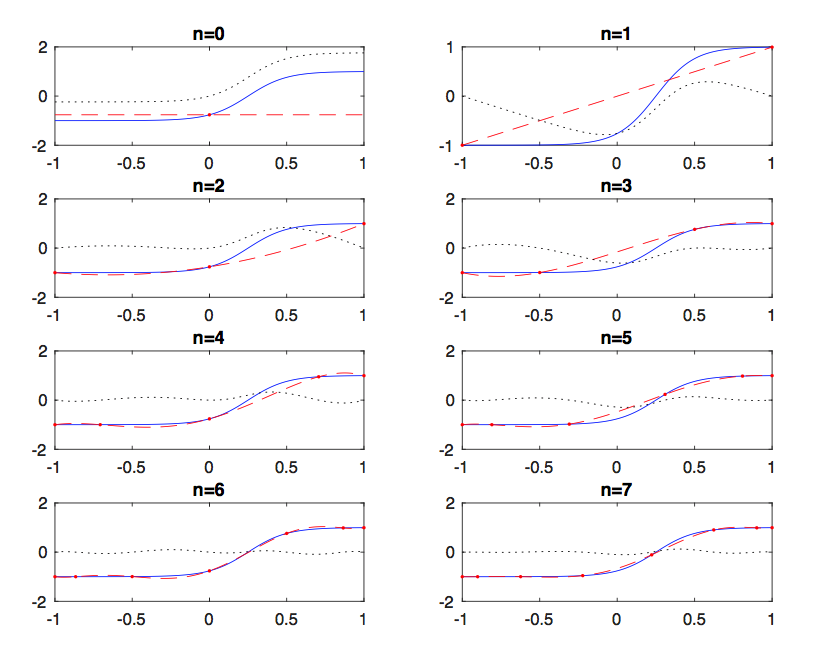
\includegraphics[width=15cm]{./Figures/20170926-interpolation-simulation}
  \label{fig:poly-interpolation-simulation}
%
%  \small{}
\end{figure}

\begin{verbatim}
x = chebfun('x');
f = tanh (4 * x -1);
n0=0;n1=1;n2=2;n3=3;n4=4;n5=5;n6=6;n7=7;
pn0 = chebfun(f,n0+1);
pn1 = chebfun(f, n1+1);
pn2 = chebfun(f, n2+1);
pn3 = chebfun(f, n3+1);
pn4 = chebfun(f, n4+1);
pn5 = chebfun(f, n5+1);
pn6 = chebfun(f, n6+1);
pn7 = chebfun(f, n7+1);

figure(1);
subplot(4,2,1),plot(f, '-b'), hold on, plot(pn0, '.--r'), hold on, plot(f-pn0, ':k'), title('n=0'),
subplot(4,2,2),plot(f, '-b'), hold on, plot(pn1, '.--r'), hold on, plot(f-pn1, ':k'), title('n=1'),
subplot(4,2,3),plot(f, '-b'), hold on, plot(pn2, '.--r'), hold on, plot(f-pn2, ':k'), title('n=2'),
subplot(4,2,4),plot(f, '-b'), hold on, plot(pn3, '.--r'), hold on, plot(f-pn3, ':k'), title('n=3'),
subplot(4,2,5),plot(f, '-b'), hold on, plot(pn4, '.--r'), hold on, plot(f-pn4, ':k'), title('n=4'),
subplot(4,2,6),plot(f, '-b'), hold on, plot(pn5, '.--r'), hold on, plot(f-pn5, ':k'), title('n=5'),
subplot(4,2,7),plot(f, '-b'), hold on, plot(pn6, '.--r'), hold on, plot(f-pn6, ':k'), title('n=6'),
subplot(4,2,8),plot(f, '-b'), hold on, plot(pn7, '.--r'), hold on, plot(f-pn7, ':k'), title('n=7'),
\end{verbatim}

\begin{theorem}[切比雪夫截断定理]
  \label{theorem:poly-cheby-truncation-theorem}
  切比雪夫截断定理(Chebyshev truncation theorem)\index{truncation!Chebyshev \dotfill 切比雪夫截断}是指,我们用$j$次切比雪夫多项式来近似未知的原方程系统$f(x)$,近似的误差小于等于一系列未被纳入考虑的更高次切比雪夫多项式系数之和,换句话说,定义$d^j(\cdot | \theta) = \sum_{i=0}^{j} \theta_i \psi_i(x)$,则截断误差(truncation error)
  \begin{equation}
    \label{eq:poly-cheby-truncation-theorem}
    d(x) - d^j(x|\theta) \le \sum_{i=j+1}^{\infty} \left| \theta_i \right|, \quad \forall x \in [-1,1], \quad \forall j.
  \end{equation}
\end{theorem}
\begin{proof}
  略。
\end{proof}


\begin{theorem}
  第$n$次一类切比雪夫多项式$T_n(x)$有$n$个根
  \begin{equation}
    \label{eq:poly-cheby-1-roots}
    x_i = \cos \left( \frac{2 i - 1}{2 n } \pi \right), \quad i = 1,2,\ldots, n,
  \end{equation}
  并且进而可将$T_n(x)$写为
  \begin{equation}
    \label{eq:poly-cheby-1-leadcoeff-root}
    T_n(x) = k_n \Pi_{i=0}^{n} \left(x - x_i \right) = 2^{n-1}  \Pi_{i=0}^{n} \left(x - x_i \right) , \quad i=1,2,\ldots,n.
  \end{equation}
\end{theorem}
\begin{proof}
  cf. \cite[p.49]{Boyd:2001wt}。
\end{proof}


\section{AR(1)过程的离散方法}
\label{sec:pj-local-discretization}
当未来存在不确定性时,求解经济个体行为最大化的问题便涉及条件期望的计算。以消费——储蓄决策问题为例,可表示为如下贝尔曼方程(Bellman equation)
\begin{equation}
  \label{sec:pj-local-discrete-cs-problem}
  \begin{split}
    &V(a, \lambda) = \max_{\{c, a' \}} \left\{ u(c) + \beta E\left[ V(a', \lambda') | \lambda \right]\right\}, \quad \text{s.t.}\\
    & a (1+r) + \omega \exp(\lambda) = a' + c, \\
    & \lambda' = (1-\rho) \mu_{\lambda} + \rho \lambda + \varepsilon,\quad \varepsilon \sim N(0,\sigma_{\varepsilon}^2), \\
    & c \ge 0, a' > 0.
  \end{split}
\end{equation}
其中状态矩$\lambda$的无条件均值和方差为$\lambda \sim N(\mu_{\lambda}, \sigma_{\lambda}^2)$。在给定$\lambda$的情况下,$\lambda'$是一个AR(1)过程,满足条件均值和方差$\lambda' \sim N\left( (1-\rho) \mu_{\lambda} + \rho \lambda, \sigma_{\varepsilon}^2 \right)$。$\sigma_{\varepsilon}$和$\sigma_{\lambda}$的关系满足
\begin{equation*}
  \sigma_{\lambda} = \frac{\sigma_{\varepsilon}}{\sqrt{1-\rho^2}}.
\end{equation*}

在此例中,涉及条件期望的计算目标是由$f(\lambda' | \lambda)$加权后的价值方程的积分值
\begin{equation}
  \label{eq:pj-local-discrete-cond-density-def}
  E\left[ V(a', \lambda') | \lambda \right] = \int_{-\infty}^{\infty} V(a',\lambda') f(\lambda' | \lambda) d \lambda',
\end{equation}
其中$f(\lambda' | \lambda)$指给定$\lambda$的情况下,$\lambda'$的条件密度(conditional density)\index{conditional density \dotfill 条件密度}。

上式是一个与当前期状态有关的无限维度问题,需要借助数值近似算法。一个可行的近似方案,思路为:将状态空间中原本是连续的状态,离散化变为有限个点,对这些点对应的条件期望做近似。换句话说,就是将关于连续的$\lambda$的马尔科夫链,转变为离散的有限马尔科夫链,我们将新的马尔科夫链用$\tilde{\lambda}$来予以区分。有限个数的$\tilde{\lambda}$取值可以来自$\Lambda = \{ \lambda_1, \lambda_2, \ldots \lambda_n \}$集合,对应转移矩阵$P$,含有转移概率$p_{i,j}$,满足
\begin{equation*}
  p_{i,j} = Prob \left( \tilde{\lambda}' = \lambda_j | \tilde{\lambda} = \lambda_i \right), \quad i,j=1,2,\ldots,n.
\end{equation*}

通过这种方式,原本是含有条件期望的积分计算问题\eqref{eq:pj-local-discrete-cond-density-def},被转换为离散化的求和问题,可以借助计算机,用某些特定的数值算法求得。下面分别介绍三种常见算法。

\subsection{Tauchen(1986)法}
\label{sec:pj-local-discretization-tauchen86}

\cite{Tauchen:1986gi}的方法可表示如下:

首先是$\lambda$的选取。在$\Lambda$中选取均匀分布的$n$个点$\{ \lambda_1, \lambda_2, \ldots \lambda_n \}$,其中$\lambda_{1}$和$\lambda_n$分别对应上下边界,值等于无条件均值$\mu_t$加上或减去无条件标准差$\sigma_{\lambda}$的$m$倍数
\begin{align*}
  &\lambda_1 = \mu_{\lambda} - m \sigma_{\lambda},\\
  &\lambda_2 = \mu_{\lambda} + m \sigma_{\lambda},
\end{align*}
经验研究中,$m$的取值通常在2到3之间。

随后是转移矩阵$P$的选取。设
\begin{equation*}
  \omega = \lambda_j - \lambda_{j-1},
\end{equation*}
进而
\begin{equation*}
  p_{i,j} = \begin{cases}
  Prob \left[ (1-\rho) \mu_{\lambda} + \rho \lambda_{i} + \varepsilon \le \lambda_{\{j=1\}}  + \frac{\omega}{2} \right] & \text{如果} j=1,\\
  Prob \left[
  \lambda_j - \frac{\omega}{2} \le (1-\rho) \mu_{\lambda} + \rho \lambda_{i} + \varepsilon \le \lambda_j + \frac{\omega}{2}
  \right] & \text{如果} j=2,3,\ldots,n-1,\\
  1-Prob \left[ \lambda_{\{j=n\}} + \frac{\omega}{2} \le (1-\rho) \mu_{\lambda} + \rho \lambda_{i} + \varepsilon  \right] & \text{如果} j=n.
  \end{cases}
\end{equation*}

上式进一步整理为
\begin{equation*}
  p_{i,j} = \begin{cases}
  \Phi \left( \frac{\lambda_1 + \frac{\omega}{2} - (1-\rho) \mu_{\lambda} - \rho \lambda_i}{\sigma_{\varepsilon}}\right) & \text{如果} j=1,\\
  \Phi \left(
  \frac{
  \lambda_j + \frac{\omega}{2} - (1-\rho) \mu_{\lambda} - \rho \lambda
  }{
  \sigma_{\varepsilon}
  } \right) -
  \Phi \left(
  \frac{
  \lambda_j - \frac{\omega}{2} - (1-\rho) \mu_{\lambda} - \rho \lambda
  }{
  \sigma_{\varepsilon}
  } \right)
   & \text{如果} j=2,3,\ldots,n-1,\\
  1- \Phi \left(
  \frac{
  \lambda_n - \frac{\omega}{2} - (1-\rho) mu_{\lambda} - \rho \lambda
  }{\sigma_{\varepsilon}}
  \right)& \text{如果} j=n,
  \end{cases}
\end{equation*}
其中$\Phi(\cdot)$表示标准正态累积分布函数(standard normal cumulative distribution function)。

\cite{Tauchen:1986gi}法,将$\tilde{\lambda}'|\tilde{\lambda} = \lambda_i$作为对$ \lambda'|\lambda = \lambda_i$的条件概率的离散近似。$n$越大,对节点的选取越密,近似的效果越精确。\cite{Tauchen:1986gi}指出当$n=9$时所获得的近似精度基本已能满足经验研究的一般需要\footnote{然而随着外生过程的持续性越来越强(high persistence)即$\rho \rightarrow 1$,近似的精度就越来越低,这就需要我们提高$n$的数量以弥补精度的下降,或是采取更适合离散化高持续性过程的算法,如第\ref{sec:pj-local-discretization-rouwenhorst95}节的\cite{Rouwenhorst:1995tq}法。}。

举例说明。对于一个随机AR(1)连续过程
\begin{equation*}
  z_t = 0.95 z_{t-1} + \varepsilon_t
\end{equation*}
以及正态分布$N(0,0.007^2)$而言,假定我们想要对它做离散化近似,对应$n=9$个点,$m=3$。

我们可以根据\cite{Tauchen:1986gi}的思路编写代码,或者使用现有程序。以Matlab为例,Iskander Karibzhanov在他的个人主页\footnote{\url{http://karibzhanov.com}。}提供了名为tauchen.m的程序。Matlab代码如下
\begin{verbatim}
  >> [y,P,d]=tauchen(5,0,0.95,0.007,3)

  y =

     -0.0673   -0.0336         0    0.0336    0.0673


  P =

      0.9727    0.0041    0.0000    0.0000    0.0000
      0.0273    0.9806    0.0082    0.0000    0.0000
      0.0000    0.0153    0.9837    0.0153    0.0000
           0    0.0000    0.0082    0.9806    0.0273
           0         0    0.0000    0.0041    0.9727


  d =

      0.0361    0.2392    0.4494    0.2392    0.0361
\end{verbatim}

即,我们得到了
\begin{equation*}
  z_t \in \left\{ -0.0673,   -0.0336,         0,    0.0336,    0.0673 \right\}
\end{equation*}

对应转移矩阵$P$
\begin{equation*}
P_{z,z'}=  \begin{pmatrix}
0.9727&    0.0041&    0&    0&    0\\
0.0273&    0.9806&    0.0082&    0&    0\\
0&    0.0153&    0.9837&    0.0153&    0\\
0&    0&    0.0082&    0.9806&    0.0273\\
0&         0&    0&    0.0041&    0.9727,
  \end{pmatrix}
\end{equation*}
需要注意的是$P_{z,z'}$对角元素接近于1,这说明随机过程的当期状态与上期状态高度相关(对应$\rho = 0.95$)。\cite{Tauchen:1986gi}增加$n$的值到9后,相关度仍然比较高(见下),这需要我们探讨其他数值算法,见第\ref{sec:pj-local-discretization-rouwenhorst95}节。

\begin{verbatim}
  >> [y,P,d]=tauchen(9,0,0.95,0.007,3)

  y =

     -0.0673   -0.0504   -0.0336   -0.0168         0    0.0168    0.0336    0.0504    0.0673


  P =

      0.7644    0.0592    0.0001    0    0    0    0    0    0
      0.2347    0.7405    0.0747    0.0001    0    0    0    0    0
      0.0009    0.1997    0.7569    0.0931    0.0002    0    0    0    0
      0    0.0006    0.1679    0.7669    0.1147    0.0002    0    0    0
      0    0    0.0004    0.1396    0.7702    0.1396    0.0004    0    0
           0    0    0    0.0002    0.1147    0.7669    0.1679    0.0006    0
           0         0    0    0    0.0002    0.0931    0.7569    0.1997    0.0009
           0         0         0    0    0    0.0001    0.0747    0.7405    0.2347
           0         0         0         0         0    0    0.0001    0.0592    0.7644


  d =

      0.0108    0.0428    0.1144    0.2064    0.2513    0.2064    0.1144    0.0428    0.0108

\end{verbatim}

即,我们得到了
\begin{equation*}
  z_t \in \left\{ -0.0673 ,  -0.0504,   -0.0336,   -0.0168,         0,    0.0168,    0.0336,    0.0504,    0.0673 \right\},
\end{equation*}
对应转移矩阵$P$
\begin{equation*}
P_{z,z'} = \begin{pmatrix}
0.7644&    0.0592&    0.0001&   0&    0&    0&    0&    0&    0 \\
0.2347&    0.7405&    0.0747&    0.0001&    0&    0&    0&    0&    0 \\
0.0009&    0.1997&    0.7569&    0.0931&    0.0002&    0&    0&    0&    0\\
0&    0.0006&    0.1679&    0.7669&    0.1147&    0.0002&    0&    0&    0\\
0&    0&    0.0004&    0.1396&    0.7702&    0.1396&    0.0004&    0&    0\\
0&    0&    0&    0.0002&    0.1147&    0.7669&    0.1679&    0.0006&    0\\
0&         0&    0&    0&    0.0002&    0.0931&    0.7569&    0.1997&    0.0009\\
0&         0&         0&    0&    0&    0.0001&    0.0747&    0.7405&    0.2347\\
0&         0&         0&         0&         0&    0&    0.0001&    0.0592&    0.7644\\
\end{pmatrix}
\end{equation*}



\subsection{Tauchen and Hussey (1991)法}
\label{sec:pj-local-discretization-th91}

同样对矩$\lambda$
而言,\cite{Tauchen:1991iv}使用高斯——埃米特求积(Gauss-Hermite quadrature)\index{Gauss-Hermite quadrature \dotfill 高斯——埃米特求积}去近似价值方程的条件期望积分,\eqref{eq:pj-local-discrete-cond-density-def}改写为
\begin{equation}
  \label{eq:pj-local-discrete-cond-density-gauss}
  E \left[ V(a', \lambda') | \lambda \right] \approx \frac{1}{\sqrt{\pi}} \sum_{j=1}^{n} \omega_j V(a', \sqrt{2} \sigma_\lambda \hat{\lambda}'_j + \mu_\lambda), \quad j=1,2,\ldots, n
\end{equation}
其中$ \hat{\lambda}'_j$是第$n$次埃米特多项式$H_n(\lambda)$的根(第\ref{sec:poly-hermite}节),满足
\begin{equation*}
  \lambda_j = \sqrt{2} \sigma_{\varepsilon} \hat{\lambda}_j + \mu_{\lambda},
\end{equation*}
$\omega_j$是对应$\hat{\lambda}'_j$的权重。

研究目标与\eqref{eq:pj-local-discrete-cond-density-def}相同:给定$\lambda$的情况下有AR(1)过程$\lambda'$,计算加权价值方程积分
\begin{equation*}
  E\left[ V(a', \lambda') | \lambda \right] = \int_{-\infty}^{\infty} V(a',\lambda') f(\lambda' | \lambda) d \lambda'.
\end{equation*}

原本可以采用上节\ref{sec:pj-local-discretization-tauchen86}介绍的\cite{Tauchen:1986gi}算法做近似求解,但需注意$\lambda'$的条件均值是一个关于$\lambda$的方程,这意味着对于每个不同的$\lambda$,都会有一组不同的$\lambda'$,进而迭代算出的集合$\Lambda$可能有无数个。为了避免这个问题,\cite{Tauchen:1991iv}建议使用如下转换
\begin{equation*}
\begin{split}
    E\left[ V(a', \lambda') | \lambda \right] &= \int_{-\infty}^{\infty} V(a',\lambda') f(\lambda' | \lambda) d \lambda'\\
    &= \int_{-\infty}^{\infty} V(a',\lambda') \frac{
    f(\lambda' | \lambda)
    }{f(\lambda' | \mu_{\lambda})}
    f(\lambda' | \mu_{\lambda}) d \lambda'.
\end{split}
\end{equation*}
其中$f(\lambda' | \mu_{\lambda})$表示在$\lambda$恰好等于其无条件均值$\mu_{\lambda}$的情况下,$\lambda'$的条件密度。将高斯——埃米特求积\eqref{eq:pj-local-discrete-cond-density-gauss}代入上式,可得
\begin{equation}
  \label{eq:pj-local-discrete-th1991-mid}
  \begin{split}
    &E\left[ V(a', \lambda') | \lambda \right] \approx
    \frac{1}{\sqrt{\pi}} \sum_{j=1}^{n} \omega_j V(a', \lambda_j) \frac{f(\lambda_j | \lambda)}{f(\lambda_j | \mu_{\lambda})}, \quad \text{其中} \\
    & \quad \lambda_j = \sqrt{2} \sigma_{\varepsilon} \hat{\lambda}_j + \mu_{\lambda}, \\
    & \quad \hat{\lambda}_j, j=1,2,\ldots,n \, \text{表示第n次埃米特多项式的根}, \\
    & \quad \omega_j \text{表示第n次埃米特多项式的根对应的权重}.
  \end{split}
\end{equation}

那么,对于$\lambda = \lambda_i$,我们有
\begin{equation}
  \label{eq:pj-local-discrete-th1991-midd}
  E \left[ V(a', \lambda' | \lambda) \right] \approx \sum_{j=1}^{n} \tilde{\omega}_{i,j} V(a', \lambda_i), \quad \tilde{\omega}_{i,j}= \frac{1}{\sqrt{\pi}} \omega_j \frac{
  f(\lambda_j | \lambda_i)
  }{
  f(\lambda_j | \mu_{\lambda})
  },
\end{equation}
上式意味着,我们选取$\tilde{\lambda}$的可能集合为
\begin{equation*}
  \Lambda = \left\{ \tilde{\lambda} | \lambda = \sqrt{2} \sigma_{\varepsilon} \hat{\lambda}_j, \, j=1,2,\ldots,n \right\},
\end{equation*}
选取$\tilde{w}$的可能集合为转移矩阵$P$:需要注意的是
\begin{equation*}
  \sum_{j=1}^{n} \tilde{\omega}_{i,j} \neq 1,
\end{equation*}
因此$P$中的元素
\begin{equation*}
  p_{i,j} = \frac{
  \tilde{\omega}_{i,j}
  }{
  \sum_{j=1}^{n} \omega_{i,j}
  }.
\end{equation*}

\eqref{eq:pj-local-discrete-th1991-midd}因此最终改写为
  \begin{equation}
    \label{eq:pj-local-discrete-th1991}
    E \left[ V \left( a', \tilde{\lambda}' | \lambda_i \right) \right] \approx \sum_{j=1}^{n} p_{i,j} V \left( a',\lambda_j \right).
  \end{equation}

由\eqref{eq:pj-local-discrete-th1991}可见,利用\cite{Tauchen:1991iv}近似条件期望用到高斯——埃米特求积的知识,但在实际计算过程中并不需要做高斯——埃米特求积\footnote{然而随着$n \rightarrow \infty$,我们有
\begin{equation*}
\lim_{n \rightarrow \infty} \sum_{j=1}^{n} \tilde{\omega}_{i,j} \rightarrow 1, \quad \forall i = 1,2,ldots,n,
\end{equation*}
因此\eqref{eq:pj-local-discrete-th1991}的\cite{Tauchen:1991iv}算出的条件期望近似依然是向高斯——埃米特求积法\eqref{eq:pj-local-discrete-cond-density-gauss}收敛的。}。

与\cite{Tauchen:1986gi}法相比,\cite{Tauchen:1991iv}的不同在于权重方程改用条件密度$\omega \left( \lambda' \right) = f \left( \lambda' | \mu_{\lambda} \right)$,如\eqref{eq:pj-local-discrete-th1991-mid}。与无条件密度相比,有条件密度在区间的中央赋予更多权重,在区间的两端赋予更小权重。这样一来,有条件密度作为权重方程,可以更好平衡两组互相冲突的原则:第一,一个好的近似总是会在无条件均值附近留下较多权重,第二,一个好的近似总是会使得在区间的两端,$\frac{f\left( \lambda' | \lambda \right)}{\omega(\lambda')}$比值不至于相对于$w(\lambda')$而增长过快。

Iskander Karibzhanov也提供了名为tauchenHussey.m的Matlab程序。

\subsection{Rouwenhorst(1995)法}
\label{sec:pj-local-discretization-rouwenhorst95}

如前文所述,对于高持续性$\rho \rightarrow 1$(如$\rho=0.9$)的过程来说,\cite{Tauchen:1986gi}近似法的精度较低。\cite{Kopecky:2010du}研究发现\cite{Rouwenhorst:1995tq}法在此时更为理想。

在区间$[\mu_{\lambda} - \nu, \mu_{\lambda} + \nu]$内选取对称且均匀分布的$n$个点构成$\Lambda$。用如下方法计算$P$:通过选择$p$和$p$,使得当时
\begin{equation*}
P_{n=2} = \begin{pmatrix}
p & 1-p \\
1-1 & q
\end{pmatrix}, \quad P_{n=3} = \begin{pmatrix}
p^2 & 2p (1-q) & (1-p)^2 \\
p(1-q) & pg + (1-p)(1-q) & q(1-p)\\
(1-q)^2 & 2q(1-p) & q^2
\end{pmatrix},
\end{equation*}
进而用递归方法,根据$P_{n-1}$计算$P_n$,分两步。首先将$n \times n$矩阵相加
\begin{equation*}
  p \begin{pmatrix}
    P_{n-1} & \bm{0} \\
    \bm{0}^{\top} & 0
    \end{pmatrix}
    + (1-p) \begin{pmatrix}
    \bm{0} & P_{n-1} \\
    0 & \bm{0}^{\top}
    \end{pmatrix},
\end{equation*}

\begin{equation*}
    (1-q) \begin{pmatrix}
    \bm{0}^{\top} & 0\\
    P_{n-1} & \bm{0}
    \end{pmatrix}
    + q \begin{pmatrix}
    0 & \bm{0}^{\top} \\
    \bm{0} & P_{n-1}
    \end{pmatrix},
\end{equation*}
随后将除了第一和最后一行之外的其他行都除以2。这样矩阵$P_n$的条件概率之和等于1。

$p^{n-1}$表示当期已处于最低状态时,下期仍处在最低状态的概率;$q^{n-1}$表示当期已处于最高状态时,下期仍处在最高状态的概率。$ (1-p)^{n-1} $表示当期已处于最低状态时,下期由最低转为最高状态的概率;$ (1-q)^{n-1} $表示当期已处于最高状态时,下期由最高转为最低状态的概率。对于任何$p \neq q$的情况,都会导致生成的冲击序列中出现异方差(heteroscedasticity)。

不论$n$和$\Lambda$的取值是怎样的,$\tilde{\lambda}$过程的一届序列相关性总是$p+q-1$。因此,如果我们设定$p+q = \pi$,就可以使得所生成的离散过程,具有和连续过程相同的一阶持续性$\rho$。

此外,$\tilde{\lambda}$的方差也总是$\frac{\nu^2}{n-1}$。因此对于某个给定的$n$值,1个合适的$\nu$值取值是使得\begin{equation*}
var \left( \tilde{\lambda} \right) = var \left( \lambda \right) \quad \Rightarrow \nu = \left( \frac{n-1}{\rho^2 - 1} \right)^{\frac{1}{2}} \sigma_{\varepsilon}.
\end{equation*}

Iskander Karibzhanov的matlab代码:

\begin{verbatim}
  >> rouwenhorst(0.95,0.007,5)

  ans =

     -0.0448   -0.0224         0    0.0224    0.0448

  >> rouwenhorst(0.95,0.007,7)

  ans =

     -0.0549   -0.0366   -0.0183         0    0.0183    0.0366    0.0549

  >> rouwenhorst(0.95,0.007,9)

  ans =

     -0.0634   -0.0476   -0.0317   -0.0159         0    0.0159    0.0317    0.0476    0.0634
\end{verbatim}

%\end{subappendices}

%!TEX root = ../DSGEnotes.tex
%\begin{subappendices}
\section{伽辽金近似}
\label{sec:pj-galerkin-approximation}

\subsection{举例:1维空间中的伽辽金近似}
\label{sec:pj-galerkin-1d-example}
以一个1维空间的有界极值问题为例,介绍伽辽金近似法(Galerkin approximation method)\index{Galerkin method \dotfill 伽辽金近似法}。假定$u(x)$是下述方程系统的解
\begin{equation}
  \label{eq:pj-galerkin-value-problem-1d}
  \begin{cases}
    -u'' + u = f, \quad \text{in} (0,1) \\
    u(0)=u(1)=0,
  \end{cases}
\end{equation}
我们的目标是找到一个对$u$的近似解。对上式两侧乘以一个检验方程$\nu$,然后分段积分,可得\eqref{eq:pj-galerkin-value-problem-1d}的弱条件形式\todo{弱条件补一个reference}
\begin{equation}
  \label{eq:pj-galerkin-value-problem-integral}
  \int_{0}^{1} \left( u' \nu' + u \nu \right) \, dx = \int_{0}^{1} f \, \nu dx, \quad \forall \nu \in H_{0}^1(0,1),
\end{equation}
 其中$ H_{0}^{1}(0,1) $是索伯列夫空间(Sobolev space)\index{Sobolev space! \dotfill 索伯列夫空间}。

如果方程$u$是常规方程,即连续且二阶可导\todo{补一个reference},那么\eqref{eq:pj-galerkin-value-problem-1d}与\eqref{eq:pj-galerkin-value-problem-integral}等价。这意味着我们可以利用\eqref{eq:pj-galerkin-value-problem-integral},构建一个多项式近似$u$。
将域$\left[ 0,1 \right]$划分为$N+1$个均匀分布(uniform distribution)的子域,每个域对应子空间$(x_j,x_{j+1})$,满足
 \begin{equation*}
   x_j = \frac{j}{N+1} \quad j=0,1, %\ldots,N+1.
 \end{equation*}

此外,定义一个包含检验方程$\nu$的空间$V_N$,满足
\begin{equation*}
  V_N = \left\{ \nu \in C^{0} : \nu |_{x_j,x_{j+1}} \text{是线性方程,并且  } \nu(0) = \nu(1) = 0 \right\},
\end{equation*}
其中$C^{0}$表示连续方程的空间。

$V_N$满足如下特征:首先,$V_N$是个有限维度空间,$N < \infty$。其次,$V_N \subset H_0^1(0,1) \, \forall N$。事实上,$\nu(x) \in V_N$由且仅由他所对应的有限个数的点$(x_1,x_2,\ldots,x_N)$所决定。

定义一个伽辽金近似方程$u_N \in V_N$作为对$u$的近似,代入\eqref{eq:pj-galerkin-value-problem-integral},我们有
\begin{equation}
  \label{eq:pj-galerkin-value-problem-approximate}
  \int_{0}^{1} \left( u_N' \nu' + u_N \nu \right) \, dx = \int_{0}^{1} f \, \nu \, dx, \quad \forall \nu \in V_N,
\end{equation}

由下节可知,存在且只存在一个$u_N$方程满足\eqref{eq:pj-galerkin-value-problem-approximate}条件\todo{解的存在性和唯一性}。并且由于$V_N$是个有限维度空间,因此$u_N$可以通过一些线性方程系统求解方法算得。基方程$\psi_j \in V_N$可以采取不同形式,例如可以选拉格朗日多项式(Lagrange polynomial)\index{polynomial!Lagrange \dotfill 拉格朗日多项式}
\begin{equation}
  \label{eq:pj-galerkin-psi-kronecker}
  \psi_j(x_i) = \delta_{ij}, \quad i,j=1,2,\ldots,N,
\end{equation}
其中$\delta_{ij}$表示克罗内克乘积。因此我们有近似方程
\begin{equation}
  \label{eq:pj-galerkin-approx-fun}
  u_N = \sum_{j=1}^{N} U_j \psi_j, \quad U_j \in \mathbb{R},
\end{equation}
其中$U_j := u_N(x_j)$。

既然任何一个检测方程$\nu \in V_N$都与$\psi_j$呈线性组合关系,\eqref{eq:pj-galerkin-value-problem-approximate}等价于
\begin{equation}
  \label{eq:pj-galerkin-value-problem-nupsik}
  \int_{0}^{1} \left( u_N' \psi_k' + u_N \psi_k \right) \, dx = \int_{0}^{1} f \, \psi_k \, dx, \quad k=1,2,\ldots,N.
\end{equation}

再引入\eqref{eq:pj-galerkin-approx-fun},替换上式LHS中的$u_N$,我们有
\begin{equation}
  \label{eq:pj-galerkin-value-problem-nupsik-uj}
  \sum_{j=1}^{N} U_j \int_{0}^1 \left( \psi_j' \psi_k' + \psi_j \psi_k \right) \, dx = \int_{0}^{1} f \, \psi_k \, dx, \quad k=1,2,\ldots,N.
\end{equation}

\eqref{eq:pj-galerkin-value-problem-nupsik-uj}构成一个$N$个方程的线性系统
\begin{equation}
  \label{eq:pj-galerkin-linear-sys}
\begin{split}
  A U = F&,\\
  &\begin{cases}
    \text{系数矩阵 } \, A=\left( a_{kj} \right) \in \mathbb{R}^{N \times N},& a_{kj} = \int_{0}^1 \left( \psi_j'\psi_k' + \psi_j \psi_k \right) \, dx,\\
    \text{系数矩阵 } \, F=\left( F_k \right) \in \mathbb{R}^{N}, & F_k = \int_{0,1}f \, \psi_k d_x,\\
    \text{待求解矩阵 } \, U=(U_j) \in \mathbb{R}^{N}
  \end{cases}
\end{split}
\end{equation}
通过求解线性方程系统\eqref{eq:pj-galerkin-linear-sys},可得矩阵$U$的解,进而根据\eqref{eq:pj-galerkin-approx-fun}可得$u_N$的值。


通过观察$\psi_j(x_i)$的性质\eqref{eq:pj-galerkin-psi-kronecker}可见,矩阵$A$是个对称的三角对角矩阵,对角元素及其附近不等于$0$的元素分别为
\begin{equation*}
  \begin{cases}
    a_{jj} = \frac{2}{h} + \frac{2}{3} h, \\
    a_{jj-1} = a_{jj+1} = -\frac{1}{h} + \frac{h}{6},
  \end{cases}
\end{equation*}
由此,待求解方程系统为$N+1$个等式
\begin{equation*}
  \begin{cases}
    U_0 := 0, \\
    \frac{-U_{j-1} + 2U_j - U_{j+1}}{h} + \frac{h}{6} U_{j-1} + \frac{2}{3} h U_j + \frac{h}{6} U_{j+1} = F_j, \quad j=1,2,\ldots,N,\\
    U_{j+1} := 0.
  \end{cases}
\end{equation*}
矩阵$A$是对称正定的(即$C^{\top} A C >0 \, \forall C \neq 0 $;由$a_{ij}$积分项中的双线性形式推得),由此可得$A$是可逆矩阵。因此,$U$进而$u_N$的解是唯一的\todo{解的存在性和唯一性}。

上式中两侧同时除以$h$,我们得到\eqref{eq:pj-galerkin-value-problem-1d}的有限差分近似形式
\begin{equation*}
  \underbrace{\frac{-U_{j-1} + 2U_j - U_{j+1}}{h^2}}_{\approx u''(x_j)} + \underbrace{\frac{1}{6} U_{j-1} + \frac{2}{3} U_j + \frac{1}{6} U_{j+1}}_{\approx u(x_j)} = \underbrace{\frac{1}{h}F_j}_{\approx f(x_j)}, \quad j=1,2,\ldots,N,
\end{equation*}
也就是说,在这个1维空间的例子中,伽辽金近似法就是将原求解问题转换为一个已知数量$N$的有限差分近似问题。

收敛问题。对于给定数量$N$,我们定义一个伽辽金近似$u_N \in V_N$,作为对原方程系统$u$的近似。随着$N \rightarrow \infty$,正交多项式的级数逐渐增加,可用来近似任何连续方程。换句话说,当空间集合$V_N$以如下方式近似$u$时,伽辽金近似$u_N$逐渐收敛至$u$:
\begin{equation*}
  \lim_{N \rightarrow \infty} ||u-v|| = \lim_{N \rightarrow \infty} \inf_{\nu \in V_{N} } ||u-v|| \rightarrow 0.
\end{equation*}

\subsection{伽辽金近似}
\label{sec:pj-galerkin-general}
第\ref{sec:pj-galerkin-1d-example}节以1维空间为例介绍了伽辽金近似的基本思路和方法。这节我们从1维扩展到通用情况,即在一个希尔伯特空间(Hilbert space)\index{Hilbert space \dotfill 希尔伯特空间}中,双线性形式下的伽辽金近似法\todo{补一个描述:Hilbert space}。

将一个希尔伯特空间定义为$V$,在其中定义一个双线性形式的连续方程$a(.,.)$和一个线性方程$L$,我们的研究目标是找到一个近似解$u \in V$,求解原方程系统
\begin{equation}
  \label{eq:pj-galerkin-prob}
  a \left( u,\nu \right) = \langle L, \nu \rangle, \quad \forall \, \nu \in V,
\end{equation}
其中$\langle .,. \rangle$表示在$V'$和$V$中的双内积(duality inner product)\index{inner product!duality \dotfill 双内积}\footnote{如$\langle A,B \rangle := A'B' + A B, \, \forall (A,B) \in V, \, (A',B') \in V'$。注意和\eqref{eq:poly-inner-product-def}的定义有所区别。}下面我们来分析,为了确保$u$存在唯一解,方程$a(.,.)$所应呈现的形式,即关于强制形式(coercive forms)\index{coercive form \dotfill 强制形式}的讨论。

\begin{definition}[方程的强制形式]
  如果存在一个常数$\alpha >0$,使得满足
  \begin{equation}
    \label{pj-galerkin-coercive-form-def}
    a(u,u) \ge \alpha ||u||_{V}^2, \quad \forall u \in V,
  \end{equation}
  那么我们说方程$a(.,.)$是一个$V$空间中的强制形式。
\end{definition}

举例说明,以\eqref{eq:pj-galerkin-prob}为例,对于二阶线形椭圆方程
  \begin{equation*}
    \begin{cases}
      -\sum_{i,j=1}^{n} \frac{\partial}{\partial x_i} \left( a_{ij} \frac{\partial u}{\partial x_j} \right) = f, & \text{in} \, \Omega \subset \mathbb{R}^n,\\
      u = 0, & \text{on} \partial \Omega
    \end{cases}
  \end{equation*}
  其中系数$a_{ij} = a_{ij}(x)$是有界方程。那么存在任意$\gamma > 0$使得
  \begin{equation}
    \label{eq:pj-galerkin-variational-form}
    \gamma |\xi|^2 \le \sum_{i,j=1}^n a_{ij} \xi_i \xi_j, \quad \forall x \in \Omega, \forall \xi \in \mathbb{R}^n,
  \end{equation}
或者说,可以以\eqref{eq:pj-galerkin-prob}的形式来表述,其中
\begin{itemize}
  \item 希尔伯特空间$V$
  \begin{equation*}
    V = H_{0}^{1}(\Omega) = \left\{ \nu \in L^2(\Omega) : \frac{\partial \nu}{\partial x_j} \in L^2(\Omega), \quad j=1,2,\ldots,n, \text{以及在}\, \partial \Omega \, \text{上有} \, \nu=0 \right\},
  \end{equation*}
  \item $\nu \in V$的范数(norm) \index{norm \dotfill 范数}为
  \begin{equation*}
    || \nu ||_{H^1} = ||\nu ||_{L^2} + ||\nabla \nu ||_{L^2},
  \end{equation*}
  \item $a(u,\nu)$为
  \begin{equation*}
    a(u,\nu) = \sum_{i,j=1}^n \int_{\Omega}a_{i,j} \frac{\partial u}{\partial x_i} \frac{\partial u}{\partial x_j} \, d x,
  \end{equation*}
  \item $L$满足
  \begin{equation*}
    \langle L, \nu \rangle = \int_{\Omega} f \, \nu \, dx.
  \end{equation*}
\end{itemize}

结合椭圆方程条件\eqref{eq:pj-galerkin-variational-form}、系数$a_{ij}$的有界特性以及庞加莱不等式,可得$a$函数形式是强制且连续的。线性方程形式$L$如果满足$f \in L^2$,则我们说它是连续的。

再举一个线性弹性方程的例子。对于应变——应力关系方程
\begin{equation*}
  \begin{cases}
    - \mu \Delta \bm{u} - (\lambda + \mu) \nabla div \bm{u} = \bm{f}, & \text{in} \, \Omega \subset \mathbb{R}^3, \\
    \bm{u} = 0, & \text{on} \, \partial \Omega
  \end{cases}
\end{equation*}
其中出于简化考虑,设满足齐次狄利克雷条件(homogeneous Dirichlet condition) \index{Dirichlet condition! homogeneous 齐次狄利克雷条件}。大于$0$的系数$\lambda$和$\mu$分别为拉梅第一参数和拉梅第二参数(Lamé elasticity parameters)\index{Lamé elasticity parameters \dotfill 拉梅弹性参数}。向量方程$\bm{u}$和$\bm{f}$未知。这个问题的弱形式可以表述为带有$V = H_{0}^{1} (\Omega)^3$条件的式\eqref{eq:pj-galerkin-prob},其中$a(\bm{u},\bm{v})$满足条件
\begin{equation*}
  a(\bm{u},\bm{v}) = \int_{\Omega} \left\{ 2 \mu \varepsilon_{i,j}(\bm{u}) \varepsilon_{i,j}(\bm{v}) + \lambda \, div \bm{u} \, div \bm{v} \, \right\} \, dx, \quad \varepsilon_{i,j} := \frac{1}{2} \left( \frac{\partial \nu_i}{\partial x_j} \frac{\partial \nu_j}{\partial x_i}\right).
\end{equation*}

进而,利用科恩不等式(Korn's inequality)\index{Korn inequality \dotfill 科恩不等式},我们有双线性形式的方程$a(.,.)$ \eqref{eq:pj-galerkin-prob} 是强制形式。

方程形式$a(.,.)$ \eqref{eq:pj-galerkin-prob}的解得存在性和唯一性,可由拉克斯一密格拉蒙定理(Lax-Milgram theorem, Theorem \ref{theorem:lax-milgram-lemma})\index{Lax-Milgram theorem \dotfill 拉克斯一密格拉蒙定理}予以证明。

在此基础上,上述条件也证实了伽辽金近似方程向原方程收敛。事实上,的确存在着一些重要范例如斯托克斯公式(Stokes equations)\index{Stokes equations \dotfill 斯托克斯公式}等,其中的双线性形式方程并不是强制的,但满足一个更弱的条件,称为上极限——下极限条件(inf-sup condition) \index{inf-sup condition \dotfill 上极限——下极限条件}\footnote{关于稳态斯托克斯公式弱形式的分析,以及上极限——下极限条件,可参考Chen Long的讲义 \href{https://www.math.uci.edu/~chenlong/226/infsup.pdf}{https://www.math.uci.edu/~chenlong/226/infsup.pdf}。}。
下面先介绍上线——下线极限条件定义。在第\ref{sec:pj-galerkin-convergence-coercive}节介绍双线性形式伽辽金近似的收敛问题。

\begin{definition}[上极限——下极限关系问题]

  如果双线性形式的方程$a(u,\nu)$在$V$空间上满足条件:对于某一$\alpha > 0$,有
  \begin{subequations}
    \label{eq:pj-galerkin-inf-sup-theorem}
    \begin{equation}
      \label{eq:pj-galerkin-inf-sup-theorem-u}
      \sup_{\nu \in V} \frac{a(u,\nu)}{||\nu||_{V}} \ge \alpha ||u||_{V}, \quad \forall u \in V,
    \end{equation}
    \begin{equation}
      \label{eq:pj-galerkin-inf-sup-theorem-nu}
      \sup_{u \in V} \frac{a(u,\nu)}{||u||_{V}} \ge \alpha ||\nu||_{V}, \quad \forall \nu \in V,
    \end{equation}
  \end{subequations}
  那么我们说,它满足上极限——下极限关系。
\end{definition}
根据这一定义,我们有以下推论:
\begin{enumerate}
\item 如果$a$是对称方程,\eqref{eq:pj-galerkin-inf-sup-theorem-u}和\eqref{eq:pj-galerkin-inf-sup-theorem-nu}等价。

\item 两个方程也可以写作
\begin{equation}
  \label{eq:pj-galerkin-inf-sup-theorem-analo}
  \inf_{u \in V} \sup_{\nu V} \frac{a(u,\nu)}{||u||_{V} \, ||\nu||_{V}}.
\end{equation}

\item 如果$a$是强制方程,那么它满足上极限——下极限关系,这是由于
\begin{equation}
  \label{eq:pj-galerkin-inf-sup-theorem-coersion}
  \sup_{\nu \in V} \frac{a(u,\nu)}{||\nu||_{V}} \ge \frac{a(u,\nu)}{||u||_{V}} \ge \alpha ||u||_{V}.
\end{equation}

\item 双线性方程$a$的上极限——下极限关系可以表示为关于$a$的线性算子$A$及其伴随算子$A^{*}$,
\begin{equation*}
  A:V \rightarrow V', \quad A^{*}: V \rightarrow V',
\end{equation*}
两个算子定义为
\begin{equation*}
  \begin{split}
    &\langle Au,\nu \rangle_{V' \times V} = a(u,\nu), \\
    &\langle u,A^{*} \nu \rangle_{V' \times V} = a(u,\nu),
  \end{split}
\end{equation*}
从而\eqref{eq:pj-galerkin-inf-sup-theorem-u}-\eqref{eq:pj-galerkin-inf-sup-theorem-nu}等价于
\begin{subequations}
  \label{eq:pj-galerkin-inf-sup-injection}
  \begin{equation}
    \label{eq:pj-galerkin-inf-sup-injection-A}
    ||A u||_{V'} \ge \alpha ||u||_{V}, \quad \forall u \in V,
  \end{equation}
  \begin{equation}
    \label{eq:pj-galerkin-inf-sup-injection-Astar}
    ||A^{*} \nu||_{V'} \ge \alpha ||\nu||_{V}, \quad \forall \nu \in V.
  \end{equation}
\end{subequations}

\item 当$V=\mathbb{R}^n$时,$a$的强制性意味着,其对应的矩阵$A$正定;$a$若满足上极限——下极限关系,则$A$进一步是可逆的。
\end{enumerate}

\begin{theorem}
  \label{theorem:galerkin-approximation}
  对于连续的双线性形式方程$a$,当且仅当线性算子$A$是双射(bijective)\index{bijection \dotfill 双射}的时,$a$满足上极限——下极限关系。$A$是双射的意思是说,原方程系统\eqref{eq:pj-galerkin-prob}对于任意$L \in V$都有唯一解,进而$A$有一个连续逆(continuous inverse)\index{continuous inverse \dotfill 连续逆}, 即$||u||_{V} \le C ||L||_{V'}$  \footnote{关于连续逆,可参考讲义Li Shiu-Tang的讲义
\href{http://www.math.utah.edu/\~li/Right\%20continuous\%20inverse.pdf}{http://www.math.utah.edu/\~li/Right\%20continuous\%20inverse.pdf}。}。
\end{theorem}
\begin{proof}
  根据泛函分析的基本原理可得,对于$W \subset V$,我们定义$W^{0} \subset V'$,满足
  \begin{equation*}
    W^0 \subset \left\{ L \in V': \langle L, \nu \rangle =0, \quad \forall \nu \in W \right\},
  \end{equation*}
  那么我们有
  \begin{subequations}
    \label{eq:pj-galerkin-bijection}
    \begin{equation}
      \label{eq:pj-galerkin-bijection-A}
      (Ker A)^0 = \overline{\Im{A^{*}}},
    \end{equation}
    \begin{equation}
      \label{eq:pj-galerkin-bijection-Astar}
      (Ker A^{*})^0 = \overline{\Im{A}},
    \end{equation}
    其中$\Im{(\cdot)}$表示复数的虚部(imaginary part)\index{complex number!imaginary part \dotfill 虚部(复数)};对应地,复数的实部(real part)\index{complex number!real part \dotfill 实部(复数)}表示为$\Re(\cdot)$。
  \end{subequations}

如果假定$a$满足上极限——下极限关系,那么由\eqref{eq:pj-galerkin-inf-sup-injection-A}可得$A$是单射(injective)\index{injection \dotfill 单射}的,由\eqref{eq:pj-galerkin-inf-sup-injection-Astar}可得$A^{*}$也是单射的。进而,如果我们能证明$\Im A$是封闭集,则根据\eqref{eq:pj-galerkin-bijection-Astar}可以证明定理。

假定$A u_n \mapsto w$,则由\eqref{eq:pj-galerkin-inf-sup-injection-A}可得
\begin{equation*}
  || A(u_n - u_m) ||_{V'} \ge \alpha || u_n - u_m ||_{V},
\end{equation*}
由此可见$\{u_n\}$是一个柯西序列(Cauchy sequnce)\index{Cauchy sequnce \dotfill 柯西序列},$u_n$收敛向某一个$u \in V$,并且由$A$的连续性特征可得,$w = A u \in \Im A$。

同理可得,如果$A$是双射的,那么$A^{*}$也是双射的,$A$和$A^{*}$都有一个连续逆。因此\eqref{eq:pj-galerkin-inf-sup-theorem-u}-\eqref{eq:pj-galerkin-inf-sup-theorem-nu}成立。
\end{proof}

在此基础上,我们为原方程系统\eqref{eq:pj-galerkin-prob}作伽辽金近似解。假定在$V$空间内,我们有一个有限维度的子空间$V_N$。则对原方程系统的伽辽金近似$u_N \in V_N$可定义为
\begin{equation}
\label{eq:pj-galerkin-approximation-solution}
a(u_N,\nu) = \langle L, \nu \rangle, \quad \forall \nu \in V_N.
\end{equation}

为了让$u_N$定义良好(well defined),我们需要对$a$作出限定。根据Theorem \ref{theorem:galerkin-approximation}可得当且仅当$a$在$V_N$子空间中满足上极限——下极限关系时,伽辽金近似解$u_N$才是存在且唯一的。尤其是,伽辽金近似解$u_N$对于强制形式的方程$a$是定义良好的。

从这个角度出发,有必要指出一下两种$V$中方程形式的本质区别:一种是强制形式,另一种是满足上极限——下极限关系,但并不是强制形式的:
\begin{remark}
  \label{remark:pj-galerkin-inf-sup-problem}
  如果$a$在$V$上强制,那么它在$V$的任何一个子空间中,尤其是$V_N$中都是强制的,此时伽辽金近似解$u_N$定义完备。

  但$V$上的上极限——下极限关系,无法传导到$V$的子空间中,那么对于不满足强制性的方程形式,还需要在子空间$V_N$中重新检验,以确保$u_N$定义完备。
\end{remark}


\subsection{强制型方程形式的伽辽金近似收敛}
\label{sec:pj-galerkin-convergence-coercive}
假定我们已知双线性形式方程$a(.,.)$是连续和强制的。因此我们有
\begin{equation}
  \label{eq:pj-galerkin-convergence-M}
  a(u,\nu) \le M  \, ||u||_{V} ||\nu||_{V}, \quad \forall u,\nu \in V,
\end{equation}
其中$M$定义为一个连续性常数(continuity constant)。在采用伽辽金近似法求得近似解$u_N$后,一个自然出现的问题是:在$V_N$被恰当选取的前提下,是否会出现$\lim_{N \rightarrow \infty} u_N \rightarrow u$的收敛?

显然,如果答案是肯定的,那么
\begin{equation}
  \label{eq:pj-galerkin-convergence-question}
  d(u,V_n) = \inf_{\nu \in V_n} || u - \nu ||_{V} \rightarrow 0, \quad \text{随着} \, N \rightarrow \infty.
\end{equation}
换句话说,收敛与否的问题,等价于探讨在子空间$V_{N}$中\eqref{eq:pj-galerkin-convergence-question}是否成立\footnote{子空间$V_N$中的所有方程,都是对$u$的近似。},以及它是不是收敛的充要条件。根据齐亚引理(Céa's lemma)\index{Céa lemma, \dotfill 齐亚引理},答案是肯定的。

\begin{lemma}[齐亚引理]
  \label{lemma:pj-galerkin-cea-lemma}
  如果$a$是一个连续且强制的方程,那么我们有
  \begin{equation}
    \label{eq:pj-galerkin-cea-lemma}
    ||u - u_N || _{V} \le \frac{M}{\alpha} \inf_{\nu \in V_N} || u - \nu || _{V}
  \end{equation}
\end{lemma}
\begin{proof}
  将伽辽金近似解 \eqref{eq:pj-galerkin-approximation-solution}
  和\eqref{eq:pj-galerkin-convergence-M}联立,构成误差方程
  \begin{equation}
    \label{eq:pj-galerkin-error-function}
    a(u-u_n,\nu)=0, \quad \forall \nu \in V_N.
  \end{equation}

由\eqref{eq:pj-galerkin-convergence-M}, ,\eqref{eq:pj-galerkin-convergence-question}和 \eqref{eq:pj-galerkin-error-function}我们有
  \begin{equation*}
    \alpha ||u-u_N||^2 \le a(u-u_N, u-u_N) = a(u - u_N,u-\nu) \le M ||u-u_N||_{V} ||u-\nu||_{V},
  \end{equation*}
  因此
  \begin{equation*}
    ||u-u_N|| \le M ||u-u_N||_{V} ||u-\nu||_{V}, \forall \nu \in V_N,
  \end{equation*}
  证毕。
\end{proof}

根据齐亚引理,在子空间$V_N$中,伽辽金近似解$u_N$是对原方程系统解$u$最好的近似,它除了受一个常数影响外,但只受双线性方程$a$形式的影响,而与子空间$V_N$的情况无关。根据这一特征,我们可以引出伽辽金近似解的收敛特性。

\begin{theorem}[伽辽金近似解的收敛(强制形式)]
  \label{theorem:pj-galerkin-approximation-convergence}
  如果$a$是个连续且强制的方程,并且空间$V_N$满足  \eqref{eq:pj-galerkin-convergence-question},那么我们有
  \begin{equation*}
    \lim_{N \rightarrow \infty} u_N = u.
  \end{equation*}
\end{theorem}

来讨论一个特殊情况,$a$还额外具有对称性。那么在$V$上,$a$定义了一个标量积(scalar product),这个标量积与原方程系统相同。此时,误差方程\eqref{eq:pj-galerkin-error-function}表明伽辽金近似解$u_N$恰好就是$u$在子空间$V_N$上的正交映射,对应标量积方程$a$。此时标量积$a$所对应的范就提供了最佳近似解。并且对应地,齐亚引理中的常数项$M/\alpha$变为$\sqrt{M/\alpha}$。

\subsection{仅满足上极限——下极限关系方程形式的伽辽金近似收敛}
\label{sec:pj-galerkin-convergence-infsup}
现在假定$a$不是强制的,但满足上极限——下极限关系\eqref{eq:pj-galerkin-inf-sup-theorem-u}-\eqref{eq:pj-galerkin-inf-sup-theorem-nu}。已知原方程系统\eqref{eq:pj-galerkin-prob}有唯一解,我们来讨论一下此时伽辽金近似的收敛问题。如Remark \ref{remark:pj-galerkin-inf-sup-problem}所强调的,上极限——下极限关系无法从$V$向下传递到子空间$V_N$,因此为了让伽辽金近似是定义良好的,我们需要假定$a$也在子空间$V_N$中满足上极限——下极限关系,即存在一个系数$\beta > 0$,使得
\begin{subequations}
  \begin{equation}
    \label{eq:pj-galerkin-approx-inf-sup-u}
    \sup_{\nu \in V_N} \frac{a(u,\nu)}{||\nu||_{V}} \ge \beta ||u||_{V}, \quad \forall u \in V_N.
  \end{equation}
  \begin{equation}
    \label{eq:pj-galerkin-approx-inf-sup-nu}
    \sup_{u \in V_N} \frac{a(u,\nu)}{||u||_{V}} \ge \beta ||\nu||_{V}, \quad \forall \nu \in V_N
  \end{equation}
\end{subequations}
我们证明\eqref{eq:pj-galerkin-approx-inf-sup-u}即可。这是因为既然子空间$V_N$是有限维度的,那么一旦\eqref{eq:pj-galerkin-approx-inf-sup-u}成立,\eqref{eq:pj-galerkin-approx-inf-sup-nu}也同样成立。

收敛若要存在,需要假定$\beta$不依赖于$N$。进而,\cite{Babuska:1971fx}对齐亚引理 \ref{lemma:pj-galerkin-cea-lemma}作以扩展,据此可以对Theorem \ref{theorem:pj-galerkin-approximation-convergence}作扩展。
\begin{lemma}[扩展齐亚引理]
  \label{lemma:pj-galerkin-cea-lemma-genralization}
  如果$a$是连续方程,满足\eqref{eq:pj-galerkin-approx-inf-sup-u}的上极限——下极限关系,那么
  \begin{equation*}
    ||u - u_N||_{V} \le \left( \frac{\beta + M}{\beta}\right) \inf_{\nu \in V_N} || u - \nu ||_{V},
  \end{equation*}
  尤其是当$\beta$不依赖于$N$时,误差项中的常数也不依赖于$N$。
\end{lemma}
\begin{proof}
  取$\nu \in V_N$。由\eqref{eq:pj-galerkin-approx-inf-sup-u}及误差方程\eqref{eq:pj-galerkin-error-function}可得
  \begin{equation*}
    \beta || \nu - u_N || _{V}
    \le \sup_{w \in V_N} \frac{a(\nu - u_N, w)}{||w||_{V}}
    = \sup_{w \in V_N} \frac{a(\nu-u, w)}{||w||_{V}}
    \le M ||\nu - u||_{V}.
  \end{equation*}
\end{proof}
由此我们有收敛定理:
\begin{theorem}[伽辽金近似解的收敛(上极限——下极限形式)]
  \label{theorem:pj-galerkin-approximation-limit-convergence}
  如果$a$是个连续方程,满足上极限——下极限关系\eqref{eq:pj-galerkin-approx-inf-sup-u},$\beta$不依赖于$N$,并且子空间$V_N$满足\eqref{eq:pj-galerkin-convergence-question},那么我们有
  \begin{equation*}
    \lim_{N \rightarrow \infty} u_N = u.
  \end{equation*}
\end{theorem}

%!TEX root = ../DSGEnotes.tex
\section{数值求积(1)}
\label{sec:numerical-integration-ncrule}

我们常常需要计算一个定积分的值,如
\begin{equation*}
  \int_{a}^{b} f(x) \, \mathrm{d}x,
\end{equation*}
若直接用解析法求解较为困难,则常常采取数值积分(numerical integratation)\index{numerical integration \dotfill 数值积分}的思路,将积分式转化为有限个方程求和的方式做近似求解,如
\begin{equation}
  \label{eq:nint-num-integ-def}
  \int_{a}^{b} f(x) \, \mathrm{d} x \approx \sum_{n=1}^{N} w_{n} f \left( x_{n} \right),
\end{equation}
也即,我们在原方程的取值区间$[a,b]$中抽取$N$个点,$n=0,1,\ldots,N$的$x_{n}$值代回方程中对应值$f \left(x_{n} \right)$。$w_{n}$表示相应的权重系数。

因此,数值积分也常常称为数值求积(numerical quadrature)\index{numerical quadrature \dotfill 数值求积}。集合$\left\{ x_{n} \right\},\left\{ w_{n} \right\}$常常称为求积点(quadrature points)\index{quadrature points \dotfill 求积点}集合和求积权重(quadrature weights)\index{quadrature weights \dotfill 求积权重}集合;合适的选取$\left\{ x_{n} \right\},\left\{ w_{n} \right\}$的算法称为求积法则(quadrature rule)\index{quadrature rule \dotfill 求积法则}。对于同一个积分求解问题\eqref{eq:nint-num-integ-def}往往存在一系列法则;评价不同法则之间好坏的标准在于,看哪个法则能用最少的样本点$N$来对\eqref{eq:nint-num-integ-def}作出最精确的近似,同时确保计算成本可控,如编程难度、计算时间等。

先从最基本的牛顿——寇特斯法则开始介绍。

\subsection{牛顿——寇特斯法则}
\label{sec:nint-ncrule}
近似求解积分问题\eqref{eq:nint-num-integ-def}的基本思路是,在区间$[a,b]$中找到一个多项式方程$P(x)$来近似$f(x)$。由于多项式的求和计算往往较为简单(多项式的介绍见第\ref{sec:poly}节),这会简化\eqref{eq:nint-num-integ-def}RHS的计算时间。我们将这种思路称为牛顿——寇特斯(求积)法则(Newton—Cotes Rule)\index{Newton—Cotes Rule \dotfill 牛顿——寇特斯法则}。牛顿——寇特斯法则随着多项式的次(degree, order)而呈层级特征:使用$p$次多项式的牛顿——寇特斯法则可称为$p$阶牛顿——寇特斯法则。

如果$f$不是多项式,那么在$[a,b]$区间内寻找近似多项式$P(x)$会较为困难。一个近似方案是将空间$[a,b]$划分为$N$个子区间(对应$N+1$个点),在每个子空间中分别寻找可以近似$f$的多项式,进而将多个多项式加权求和,作为整个空间中$f$的近似方程。$N$越大,子空间的个数越多,划分就越精细,每个子空间中的近似就越精确,进而整个空间中的近似求积就越精确。

\subsubsection{矩形法则}
\label{sec:ninc-nc-rectangular-rule}
我们先从$p=0$的情况开始理解牛顿——寇特斯法则,根据黎曼求和(Riemann sums),我们可以将方程$f(x)$理解为一组矩形的集合,对$f(x)$在区间$[a,b]$中求积就是求曲线下方的面积,近似等于各个矩形面积的和。随着$N$趋近于无穷大,每个矩形的宽度无限接近于$0$,近似就越精确。

在每个子空间中分别用$1$个$p=0$次多项式来近似$f$,$0$次多项式是个常数,换句话说我们在每个子空间中用一个常数来近似$f$。这又称为矩形求积法则(rectangular quadrature rule)\index{rectangular (quadrature) rule \dotfill 矩形(求积)法则}。

\begin{figure}[htbp]
   \caption{矩形法则$(N=4)$}
  \centering
  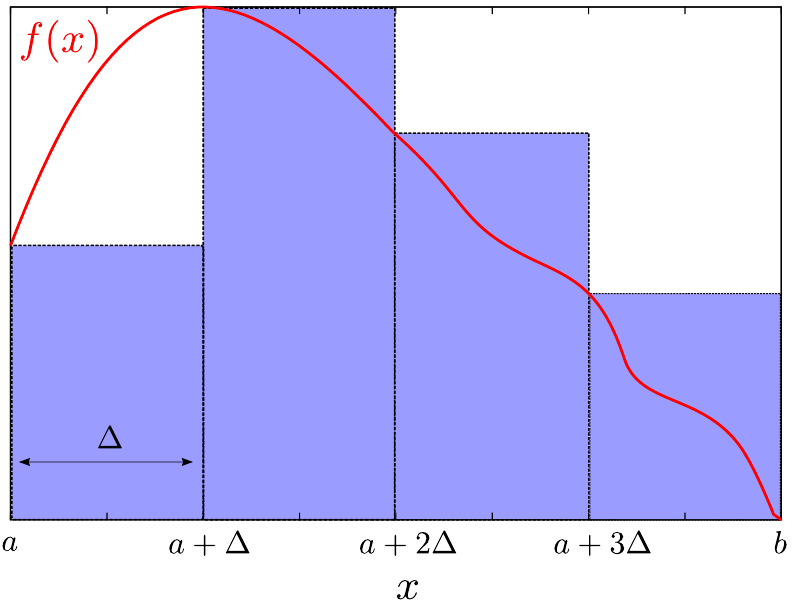
\includegraphics[width=8cm]{./Figures/20180227-rectangular-rule-example.png}
  \label{fig:ninc-nc-rectangular-rule}
%
%  \small{Source: PBOC.}
\end{figure}
图\ref{fig:ninc-nc-rectangular-rule}绘出了$N=4$情况下,利用矩形法则对$\int_{a}^{b} f(x) \, \mathrm{d}x$的近似。不难看出,将区间$[a,b]$划分为$N$个等宽子区间,每个子区间的宽度都是$\Delta = \left(b - a \right)/N$。最左侧第一个矩形,左边长(高)为$f(a)$,宽为$\Delta$,对应面积为$f(a) \cdot \Delta$。
左数第二个矩形,左边长(高)为$f \left( a+\Delta \right)$,宽也是$\Delta$,面积为$\left( a+\Delta \right) \cdot \Delta$,以此类推直到第$N=4$个矩形为止。将这些子区间中矩形的面积加总,可得矩形法则的近似表达式
\begin{equation*}
    \mathcal{I}_{N=4}^{rect}
    %\mathcal{N}_{N=4}^{rect}
    \approx
    f(a) \cdot \Delta
    + f \left(a + \Delta \right) \cdot \Delta
    + f \left(a + 2 \Delta \right) \cdot \Delta
    + f \left(a + 3 \Delta \right) \cdot \Delta,
\end{equation*}
扩展到更一般的$N \in \mathcal{N}$的情况,利用$N$段矩形法则对积分$\int_{a}^{b} f(x) \, \mathrm{d} x$的近似为
\begin{equation}
  \label{eq:ninc-nc-rectangular-rule}
  \mathcal{I}_{N}^{rect} = \sum_{n=0}^{N-1} f \left( a + n \cdot \Delta \right) \cdot \Delta.
\end{equation}

矩形法则\eqref{eq:ninc-nc-rectangular-rule}成为对\eqref{eq:nint-num-integ-def}的近似求积法则之一:
\begin{itemize}
  \item 求积权重集合$\left\{ w_{n} \right\}_{n=0}^{N-1}$对应$w_{n} \equiv \Delta \, \forall \, n$,
  \item 求积点集合$\left\{ x_{n} \right\}_{n=0}^{N-1}$对应$x_{n} = a + n \cdot \Delta, \, n = 0,1,\ldots,N-1$。
\end{itemize}

值得注意的是,在矩形法则下,我们只需要左边长,从而无需计算$f(b)$。


\subsubsection{梯形法则}
\label{sec:ninc-nc-trapezoidal-rule}
从图\ref{fig:ninc-nc-rectangular-rule}中不难看出,利用矩形法则近似曲线下方阴影的面积,近似效果并不理想。一个可能的改进方案是利用梯形代替矩形做近似,又称梯形近似法则。

在每个子空间中分别用$1$个$p=1$次多项式来近似$f$,$1$次多项式是条斜线,连接子区间的两个端点(始点和终点)。这又称为梯形求积法则(trapezoidal quadrature rule)\index{trapezoidal (quadrature) rule \dotfill 梯形(求积)法则}。

\begin{figure}[htbp]
  \caption{梯形法则$(N=4)$}
  \centering
  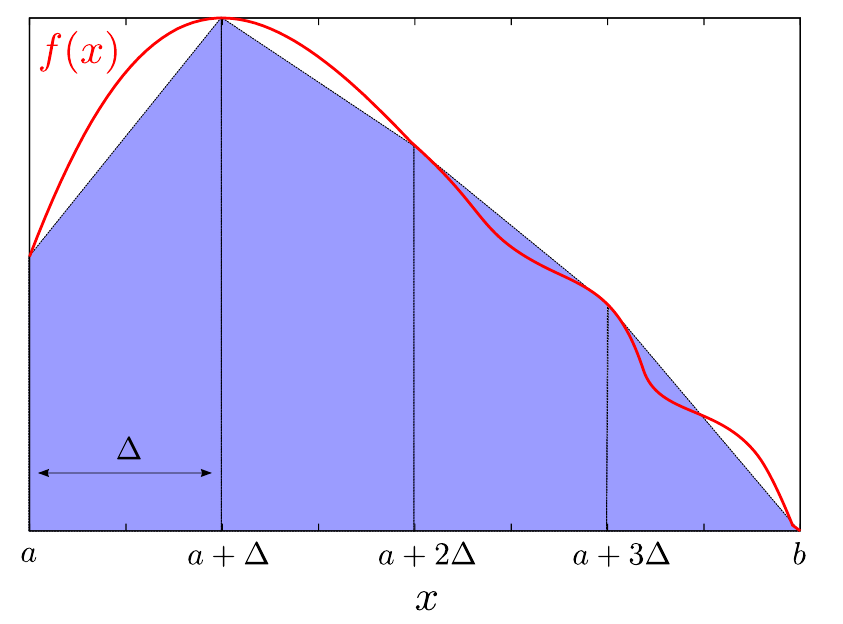
\includegraphics[width=8cm]{./Figures/20180227-trapezoidal-rule-example.png}
  \label{fig:ninc-nc-trapezoidal-rule}
%
%  \small{Source: PBOC.}
\end{figure}

见图\ref{fig:ninc-nc-trapezoidal-rule}所示,左数第$1$个梯形的面积等于
\begin{equation*}
  \frac{1}{2} \left[ f \left( a \right) + f \left( a + \Delta \right) \right] \cdot \Delta,
\end{equation*}

左数第$2$个梯形的面积等于
\begin{equation*}
  \frac{1}{2} \left[ f \left( a + \Delta \right) + f \left( a + 2 \Delta \right) \right] \cdot \Delta,
\end{equation*}
以此类推直到第$N=4$个梯形。将子区间中梯形的面积加总,可得
\begin{equation*}
\begin{split}
  \mathcal{I}_{N=4}^{trap} = &
    \frac{1}{2} \left[ f \left( a \right) + f \left( a + \Delta \right) \right] \cdot \Delta
    + \frac{1}{2} \left[ f \left( a + \Delta \right) + f \left( a + 2 \Delta \right) \right] \cdot \Delta \\
    & + \frac{1}{2} \left[ f \left( a + 2 \Delta \right) + f \left( a + 3 \Delta \right) \right] \cdot \Delta
    + \frac{1}{2} \left[ f \left( a + 3 \Delta \right) + f \left( a + 4 \Delta \right) \right] \cdot \Delta \\
    = & \left[
    \frac{1}{2} f \left( a \right)
    + f \left( a + \Delta \right)
    + f \left( a + 2 \Delta \right)
    + f \left( a + 3 \Delta \right)
    + \frac{1}{2} f \left( a + b \right)
    \right] \cdot \Delta,
\end{split}
\end{equation*}
扩展到更一般的$N \in \mathcal{N}$的情况,我们有$N$段梯形法则对$\int_{a}^{b} f \left( x \right) \, \mathrm{d} x$的近似为
\begin{equation}
  \label{eq:ninc-nc-trapezoidal-rule}
  \mathcal{I}_{N}^{trap} = \frac{1}{2} f \left( a \right) \cdot \Delta
  + \Delta \cdot \sum_{n=1}^{N-1} f \left( a + n \cdot \Delta \right)
  + \frac{1}{2} f \left( b \right) \cdot \Delta.
\end{equation}


梯形法则\eqref{eq:ninc-nc-trapezoidal-rule}称为对\eqref{eq:nint-num-integ-def}的又一种近似求积法则:
\begin{itemize}
  \item 求积点集合$\left\{ x_{n} \right\}_{n=1}^{N-1}$对应$x_{n} = a + n \cdot \Delta, \, n = 0,1,\ldots,N$,
  \item 求积权重集合$\left\{ w_{n} \right\}_{n=1}^{N}$对应
  \begin{equation*}
  w_{n} =
  \begin{cases}
  \frac{1}{2} \Delta, & n = 0, N, \\
  \Delta, & n = 1, 2, \ldots, N-1,
  \end{cases}
\end{equation*}
值得注意的是,比起矩形法则来,当利用梯形法则做近似求积时,需计算$N+1$个求积抽样点,比矩形法则多出的$1$个点为总区间中的末端$b$,对应$f(b)$。
\end{itemize}

\subsubsection{更高阶牛顿——寇特斯法则}
\label{sec:ninc-nc-higher-rule}
已知用$p=0$阶多项式(常数)近似子区间中的$f$,称矩形法则。用$p=1$阶多项式(斜线)近似,称梯形法则。那么我们可以进一步迭代计算更高阶$p > 1$的牛顿——寇特斯求积近似,方法如下
\begin{enumerate}
  \item 在子区间$\left[ x_{n}, x_{n+1} \right]$中,配$p+1$个等距离分布的点(包括子区间的起始点$x_{n}$和终结点$x_{n+1}$),将子区间分为$p$个部分。例如,
  \begin{itemize}
    \item 对$p=2$而言,配3个点$x_{n}, \frac{1}{2} \cdot \left[ x_{n} + x_{n+1} \right] , x_{n+1}$,
    \item 对$p=3$而言,配4个点$x_{n}, \frac{1}{3} \cdot \left[ x_{n} + x_{n+1} \right] , \frac{2}{3} \cdot \left[ x_{n} + x_{n+1} \right], x_{n+1}$,以此类推。
  \end{itemize}
  \item 在子空间中针对这$p+1$个配点,找到唯一的多项式$P(x)$以近似$f(x)$。例如,
  \begin{itemize}
    \item $p=0$,$P(x)$是个常数。矩形法则。
    \item $p=1$,$P(x)$是条斜线,连接子区间的两个端点$f \left( x_{n} \right), \, f \left( x_{n+1} \right)$。梯形法则。
    \item $p=2$,$P(x)$是一条经过如下3个点的抛物线,3个点的坐标依次为
    \begin{equation*}
      \begin{cases}
        \Big( x_{n}, f \left( x_{n} \right) \Big), \\
        \Big( x_{m}, f \left( x_{m} \right) \Big), \quad x_{m} \equiv \frac{x_{n} + x_{n+1}}{2}, \\
        \Big( x_{n+1}, f \left( x_{n+1} \right) \Big).
      \end{cases}
    \end{equation*}
    \item $p=3$,$P(x)$是一条经过如下4个点的曲线(图\ref{fig:ninc-nc-higher-p3}),4个点的坐标依次为
    \begin{equation*}
      \begin{cases}
        \Big( x_{n}, f \left( x_{n} \right) \Big), \\
        \Big( x_{m}, f \left( x_{m} \right) \Big), \quad x_{m} \equiv \frac{1}{3} \left( x_{n} + x_{n+1} \right), \\
        \Big( x_{m+1}, f \left( x_{m+1} \right) \Big), \quad x_{m+1} \equiv \frac{2}{3} \left( x_{n} + x_{n+1} \right), \\
        \Big( x_{n+1}, f \left( x_{n+1} \right) \Big),
      \end{cases}
    \end{equation*}
    \begin{figure}[htbp]
       \caption{3阶牛顿——寇特斯法则,对应子区间中的4个配点}
      \centering
      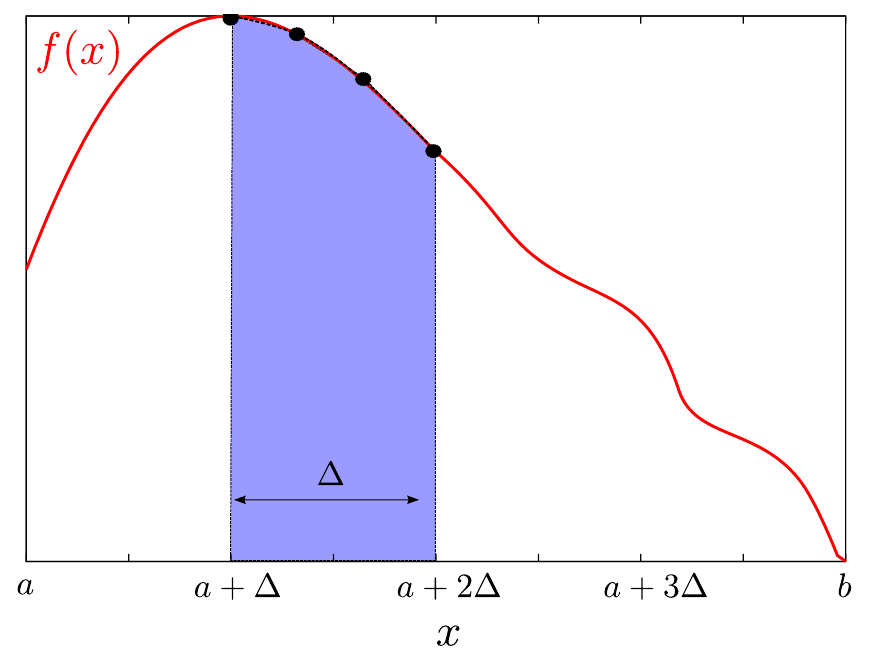
\includegraphics[width=8cm]{./Figures/20180227-nc-higher.png}
      \label{fig:ninc-nc-higher-p3}
    %
    %  \small{Source: PBOC.}
    \end{figure}
以此类推。无论哪一个例子中,$P(x)$都是这样一个多项式,其系数是抽样方程$f(x)$值的线性组合。
  \end{itemize}

  \item 从$x_{n}$到$x_{n+1}$对$P(x)$求积分,作为这个子区间内方程$f(x)$的近似。
  \item 将所有子区间内的近似方程组合起来,作为总区间中的最终近似求积法则。
\end{enumerate}

$p=2$时的牛顿——寇特斯求积,又称辛普森法则(Simpson's rule)\index{Simpson's (quadrature) rule \dotfill 辛普森(求积)法则}
\begin{equation}
  \label{eq:ninc-nc-simpson-rule}
  \mathcal{I}_{N}^{simp} =
  \sum_{n=0}^{N-1}
  \frac{\Delta}{6}
  \left[
  f \left( a + n \cdot \Delta \right)
  + 4 f \left( a + \left( n + \frac{1}{2} \right) \cdot \Delta \right)
  + f \left( a + \left( n + 1 \right)  \right) \cdot \Delta
  \right].
\end{equation}

\subsubsection{龙格现象}
\label{sec:ninc-nc-runge}
%20180227-Runge-phenomenon.png
一个自然出现的问题:更高阶的牛顿——寇特斯法则会不会带来更精确的近似解?很遗憾,答案是否定的。这是由于龙格现象(Runge phenomenon)\index{Runge phenomenon \dotfill 龙格现象}:当我们试图利用子空间中等距分布的点做更高阶多项式近似时,再查指点附近的多项式方程会出现较大幅度的震荡,从而影响最终求积估计的精确度,可参考\href{https://en.m.wikipedia.org/wiki/Runge%27s_phenomenon}{维基百科词条}。图\ref{fig:ninc-nc-higher-runge-phenomenon}中,蓝线和绿线分别表示$p=5$和$p=9$时的差值多项式近似,对应$N=6$。红线表示龙格方程(Runge function)。

\begin{figure}[htbp]
   \caption{龙格现象$(N=6)$}
  \centering
  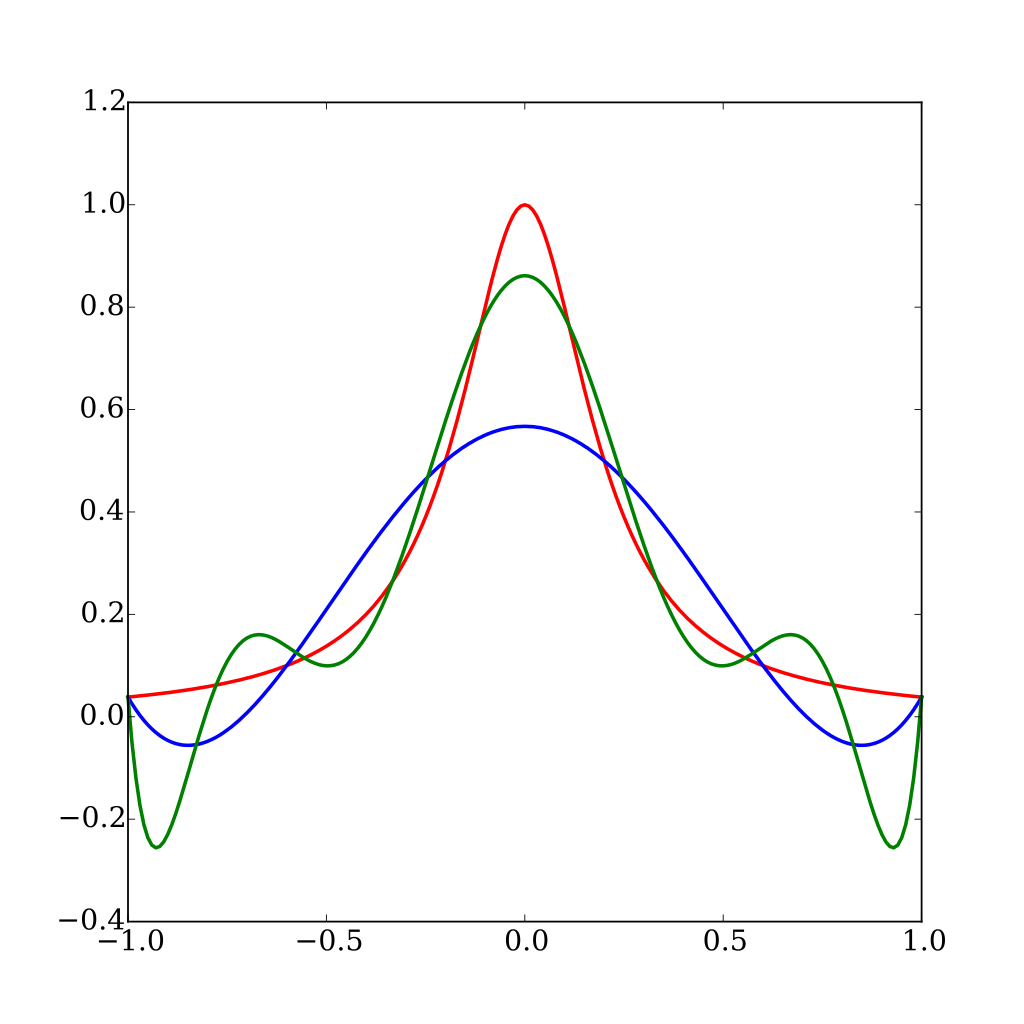
\includegraphics[width=8cm]{./Figures/20180227-Runge-phenomenon.png}
  \label{fig:ninc-nc-higher-runge-phenomenon}
%
%  \small{Source: PBOC.}
\end{figure}

\subsubsection{误差的收敛}
\label{sec:ninc-nc-error-convergence}
比较不同求积法则的优劣,可用启发式误差“分析”\footnote{加上引号是指,这种方法只是一种较为常用的检验措施,而不宜理解为某种严谨的学术性系统性表达。},观察近似误差随着配点数$N$增加的衰减速度。具体说来
\begin{enumerate}
  \item 考虑区间中某一宽度为$\Delta$的特定子区间,在其中用一个$p$阶多项式$P(x)$来近似$f$
  \begin{equation*}
    P(x) = c_{0} + c_{1} x + c_{2} x^{2} + \ldots + c_{p} x^{p}.
  \end{equation*}
  \item 那么子区间中存在一个点$x_{0}$,使得$f$围绕$x_{0}$做泰勒级数展开的前$p+1$项,与$P(x)$一致
  \footnote{例如
  \begin{itemize}
    \item $p=0$,矩形法则,$x_{0}$可以是子区间的起始点。
    \item $p=1$,梯形法则,$x_{0}$的存在性可由中值定理予以证明:$x_{n}$和$x_{n+1}$之间必然存在一点,该点上的方程值$f\left( x_{0} \right)$的导数,等于连接$f \left(x_{n} \right)$和$f \left( x_{n+1} \right)$两点的斜线的斜率。
    \item $p >1$,更高阶求和法则中$x_{0}$点存在性的证明,也可用类似思路证得。
  \end{itemize}
  }。
  可将$f$写成如下形式
  \begin{equation*}
    f(x) = \underbrace{
    c_{0} + c_{1} x + \ldots + c_{p} x^{p} }_{\equiv P(x)}
    + c_{p+1} x^{p+1} + \ldots.
  \end{equation*}
  \item 由此可见,原方程$f(x)$及其近似多项式$P(x)$之间的误差是一个从$p+1$阶开始的多项式
  \begin{equation*}
    f(x) - P(x) = c_{p+1} x^{p+1} + c_{p+2} x^{p+2} + \ldots,
  \end{equation*}
  \item 那么在这个子区间$\left[ x_{n}, x_{n+1} \right]$内的全部误差可求积得出
  \begin{equation*}
    \begin{split}
      \int \left[ f(x) - P(x) \right] \, \mathrm{d} x
      & = \int \left[
      c_{p+1} x^{p+1} + c_{p+2} x^{p+2} + \ldots \right] \, \mathrm{d} x \\
      & \propto \Delta^{p+2} + \text{更高阶项},
    \end{split}
  \end{equation*}
  最后一行是说,对$x^{p+1}$沿着某个宽度为$\Delta$的子区间求积,等于某个和$\Delta^{p+2}$成比例的值。
  \item 将一个子区间中的情况扩展到其他子区间,每个子区间中的误差项都与$\Delta^{p+2}$成定比例。更进一步地,由于$\Delta$与$N$反比例相关(N是整个区间中划分的子区间的数量)
  \begin{equation*}
    \Delta \sim \frac{1}{N},
  \end{equation*}
  那么每个子区间中的误差项可近似表示为
  \begin{equation*}
    \Delta \propto \frac{1}{N^{p+2}}.
  \end{equation*}
  \item 将$N$个子区间的误差项汇总
  \begin{equation}
    \varepsilon \propto \frac{N}{N^{p+2}} =  \frac{1}{N^{p+2}},
  \end{equation}
  例如矩形法则$(p=0)$的近似误差$\propto \frac{1}{N}$,梯形法则$(p=1)$的近似误差$\propto \frac{1}{N^{2}}$。可见误差与$N$成反比:$N$越大,划分的子区间数量越多,近似误差越小。
\end{enumerate}

举例,假定我们要用求积法则近似计算
\begin{equation*}
  \mathcal{I} = \int_{1}^{2} \log^{2} x \, \mathrm{d} x,
\end{equation*}
对应相对误差定义为$\varepsilon^{rel}$
\begin{equation*}
  \varepsilon^{rel} \equiv \frac{
  \big| \mathcal{I}_{N}^{approx} - \mathcal{I} \big|
  }{
  \mathcal{I}
  }
\end{equation*}

应用矩形法则和梯形法则,查看近似误差随着$N$增大的收敛情况如图\ref{fig:ninc-nc-error-convergence},可以看出

\begin{figure}[htbp]
   \caption{比较矩形法则和梯形法则下,近似误差随$N$值增大的收敛情况}
  \centering
  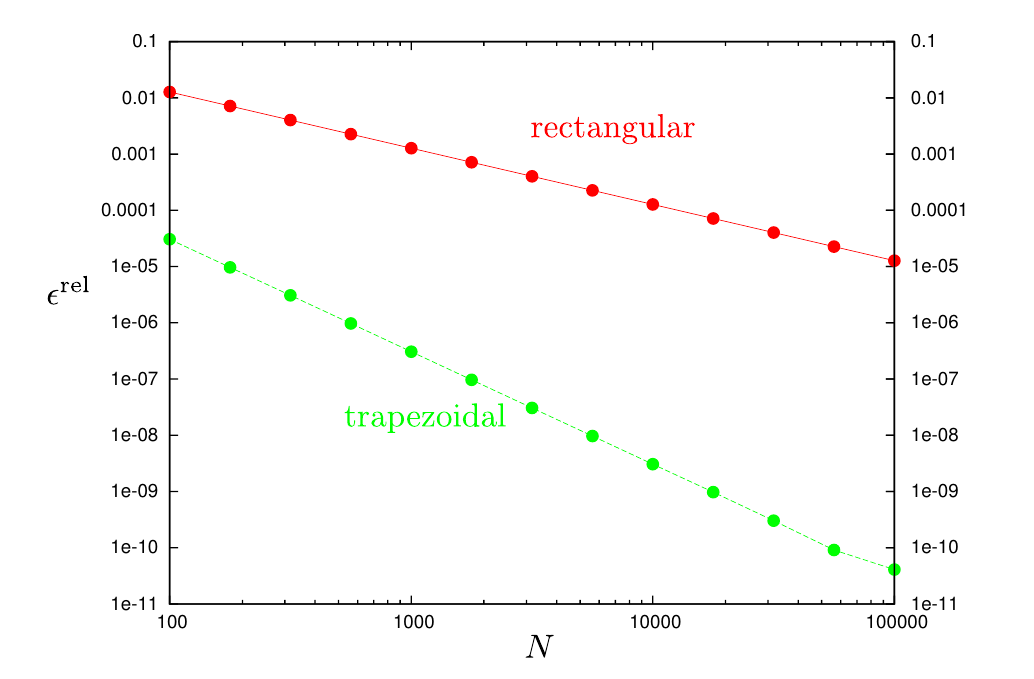
\includegraphics[width=10cm]{./Figures/20180227-nc-higher-error-convergence.png}
  \label{fig:ninc-nc-error-convergence}

  \small{原求积方程$\int_{1}^{2} \log^{2} x \, \mathrm{d} x$。}
\end{figure}

这两种方法代表的牛顿——寇特斯法则下误差项随着$N$而作线性收敛:
随着$N$增大$1,000$倍,矩形法则误差降低约$1,000$倍,$\Delta \varepsilon^{rect} \propto \frac{1}{\Delta N}$;梯形法则降低约$1,000,000$倍,$\Delta \varepsilon^{trap} \propto \frac{1}{ \left(\Delta N \right)^{2}}$。梯度法则优于矩形法则。

但图\ref{fig:ninc-nc-error-convergence}也揭示出牛顿——寇特斯法则的不足:即便是对于$\log^{2} x$这种很平滑的方程,梯形法则也需要大约$1,000$个样本,才能将总体误差控制在$10^{-6}$的水平上(为了达到类似的精度,矩形法则甚至需要$10^{6}$个样本)。从计算成本来看,牛顿——寇特斯法则恐怕不是最理想的方案,需要加以改进。如下文介绍的克伦肖——柯蒂斯法则,可以用少得多的样本量达到同样$10^{-6}$级别的误差水平,哪怕所处理的原方程更加复杂\todo{做一个ref}。

\subsection{几个小技巧}
\label{sec:ninc-tips}
以牛顿——寇特斯法则为例,介绍几个小技巧。它们对其他如克伦肖——柯蒂斯法则也适用。

\subsubsection{无限区间求积}
\label{sec:ninc-tips-improper-integral}
有时会遇到求含有无限区间的积分问题如
\begin{equation*}
  \int_{0}^{\infty} f(x) \, \mathrm{d} x,
\end{equation*}
这需要我们先将区间$[0, \infty)$映射到一个有界区间内,如
\begin{equation*}
  x:[0, \infty) \mapsto u:[0,1],
\end{equation*}
然后再应用求解定积分的求积法则。映射的方法有很多种,其中之一是设
\begin{equation*}
  x \equiv \frac{u}{1-u}, \Rightarrow \mathrm{d} x = \frac{\mathrm{d} u}{\left( 1 - u \right)^{2}},
\end{equation*}
求积问题因此转换为
\begin{equation*}
  \int_{0}^{\infty} f(x) \, \mathrm{d} x = \int_{0}^{1} \frac{1}{\left( 1 - u \right)^{2}} f
  \left( \frac{u}{1 - u} \right) \, \mathrm{d} u.
\end{equation*}

需要指出的是,上式在转换之后,含有一个奇异点(singularity):$\lim_{u \rightarrow 1} f(x) \rightarrow \infty$。然而若是在前提假设中假定$f(x)$在$x \rightarrow \infty$处消失(这个假定是为了确保积分$\int_{0}^{\infty} f(x) \, \mathrm{d} x$收敛),则这一奇异点也就不存在了。

\subsection{求积中的可积奇异点问题}
除了上节提到的情况之外,还应该注意到,有些奇异点是可积的(integrable singular points)\index{integrable singular points \dotfill 可积奇异点},例如这个求积问题
\begin{equation*}
  \mathcal{I} = \int_{0}^{1} \frac{\exp(x)}{\sqrt{x}} \, \mathrm{d} x.
\end{equation*}



\end{subappendices}

%%!TEX root = ../DSGEnotes.tex


  \subsubsection{雅各比方程}
  \label{sec:fourier-poisson-jacobian}
  雅各比方程族(Jacobian $\theta$ function)\index{Jacobian function \dotfill 雅各比方程}中的一种形式可以表示为
  \begin{equation}
    \label{eq:fourier-poisson-jacobian}
    \theta(x) = \sum_{n = - \infty}^{\infty}
    \exp \left( - n^{2} \pi x \right)
    = \sum_{n = - \infty}^{\infty} T_{x}(n).
  \end{equation}

利用泊松求和式\eqref{eq:fourier-poisson-summation-formula},以及设$\Delta t = 1$,有
\begin{equation}
  \label{eq:fourier-poisson-jacobian-2}
  \theta(x) = 2 \pi \sum_{\nu = - \infty}^{\infty} \widetilde{T} \left( 2 \nu \pi \right)
  = \frac{1}{\sqrt{x}}
  \underbrace{
  \sum_{\nu = - \infty}^{\infty}
  \exp \left(
   - \frac{\pi \nu^{2}}{x}
  \right)
  }_{= \theta \left( \frac{1}{x} \right)},
\end{equation}

即雅各比方程\eqref{eq:fourier-poisson-jacobian}的函数方程(functional equation)形式
\begin{equation}
  \label{eq:fourier-poisson-jacobian-equiv}
  \begin{split}
    \theta \left( x \right) & = \frac{1}{\sqrt{x}} \theta \left( \frac{1}{x} \right),\\
    \Leftrightarrow \sum_{n = - \infty}^{\infty}
    \exp \left( - n^{2} \pi x \right) & = x^{-\frac{1}{2}} \sum_{\nu = - \infty}^{\infty} \exp \left( - \frac{\nu^{2} \pi }{x} \right).
  \end{split}
\end{equation}

% Table generated by Excel2LaTeX from sheet 'Sheet1'
\begin{table}[htbp]
  \centering
  \caption{雅各比方程的泊松求和}
    \begin{tabular}{|l|r|rrr}
    \toprule
          & \multicolumn{2}{c|}{LHS} & \multicolumn{2}{c|}{RHS} \\
    \midrule
    $n(\nu)$ & \multicolumn{1}{l|}{$\exp \left( -n^{2} \pi x \right)$} & \multicolumn{1}{l|}{$\sum_{n} \exp \left( -n^{2} \pi x \right)$} & \multicolumn{1}{l|}{$\exp \left( -\nu^{2} \pi / x \right)$} &
    \multicolumn{1}{l|}{$\sum_{\nu} \exp \left( -\nu^{2} \pi / x \right)$} \\
    \midrule
    \multicolumn{1}{|r|}{0} & 1.000000000 & \multicolumn{1}{r|}{1.000000000} & \multicolumn{1}{r|}{1.000000000} & \multicolumn{1}{r|}{5.000000000} \\
    \midrule
    \multicolumn{1}{|r|}{1} & 0.881911378 & \multicolumn{1}{r|}{2.763822757} & \multicolumn{1}{r|}{7.77304E-35} & \multicolumn{1}{r|}{5.000000000} \\
    \midrule
    \multicolumn{1}{|r|}{2} & 0.604922563 & \multicolumn{1}{r|}{3.973667882} & \multicolumn{1}{r|}{3.6506E-137} & \multicolumn{1}{r|}{5.000000000} \\
    \midrule
    \multicolumn{1}{|r|}{3} & 0.322718983 & \multicolumn{1}{r|}{4.619105849} & \multicolumn{1}{r|}{1.0359E-307} & \multicolumn{1}{r|}{5.000000000} \\
    \midrule
    \multicolumn{1}{|r|}{4} & 0.133905721 & \multicolumn{1}{r|}{4.886917291} & \multicolumn{1}{r|}{0} & \multicolumn{1}{r|}{5.000000000} \\
    \midrule
    \multicolumn{1}{|r|}{5} & 0.043213918 & \multicolumn{1}{r|}{4.973345128} & \multicolumn{1}{r|}{0} & \multicolumn{1}{r|}{5.000000000} \\
    \midrule
    \multicolumn{1}{|r|}{6} & 0.010846711 & \multicolumn{1}{r|}{4.995038549} & \multicolumn{1}{r|}{0} & \multicolumn{1}{r|}{5.000000000} \\
    \midrule
    \multicolumn{1}{|r|}{7} & 0.002117495 & \multicolumn{1}{r|}{4.999273539} & \multicolumn{1}{r|}{0} & \multicolumn{1}{r|}{5.000000000} \\
    \midrule
    \multicolumn{1}{|r|}{8} & 0.000321512 & \multicolumn{1}{r|}{4.999916562} & \multicolumn{1}{r|}{0} & \multicolumn{1}{r|}{5.000000000} \\
    \midrule
    \multicolumn{1}{|r|}{9} & 3.79683E-05 & \multicolumn{1}{r|}{4.999992498} & \multicolumn{1}{r|}{0} & \multicolumn{1}{r|}{5.000000000} \\
    \midrule
    \multicolumn{1}{|r|}{10} & 3.48734E-06 & \multicolumn{1}{r|}{4.999999473} & \multicolumn{1}{r|}{0} & \multicolumn{1}{r|}{5.000000000} \\
    \midrule
    \multicolumn{1}{|r|}{11} & 2.49126E-07 & \multicolumn{1}{r|}{4.999999971} & \multicolumn{1}{r|}{0} & \multicolumn{1}{r|}{5.000000000} \\
    \midrule
    x=    & 0.04  &       &       &  \\
\cmidrule{1-2}    \end{tabular}%
  \label{tab:fourier-poisson-jacobian-equiv}%

  \small{注:基于式\eqref{eq:fourier-poisson-jacobian-equiv}计算。excel表格见文件夹中data/20180306-poisson.xlsx .}
\end{table}%

为了说明为何傅里叶级数求和的形式即\eqref{eq:fourier-poisson-jacobian-equiv}RHS更适于进行数值计算,我们做了一个小实验,设$x=0.04$,$n=0,1,\ldots,11$。不难看出,LHS需要$n=11$,前后23项的求和才能达到小数点后6位的精度;而对于雅各比方程形式的傅里叶级数求和,RHS只需要$n=1$就能达到同样的精度,换句话说,由\eqref{eq:fourier-poisson-jacobian-equiv}我们有
\begin{equation*}
  \underbrace{
  \theta \left( 0.04 \right)
  }_{4.999999971, n=11}
  =
  \underbrace{
  \frac{1}{\sqrt{0.04}}
  }_{5.0}
  \underbrace{
  \theta \left( \frac{1}{0.04} \right)
  }_{1.000000000, \nu = 1}
\end{equation*}

\subsection{傅里叶分析与卷积}
\label{sec:fourier-series-convolution}
傅里叶分析的又一个重要特征是,它是以卷积(convolution)\index{convolution \dotfill 卷积}乘的形式出现的。如上文所示,由两个方程$f(t)$和$g(t)$构成的卷积,近似表示为一系列$g(\tau)$的加权和,$g(\tau)$是对$g(t)$的近似(copy)之一,对应权重$f(\tau)$,我们设这个卷积为$C(t)$
\begin{equation*}
  C(t) \equiv f \times g = \int_{-\infty}^{\infty} f(\tau) g(t - \tau) d \tau.
\end{equation*}

对$C(t)$作傅里叶变换,有
\begin{equation*}
  \begin{split}
  \widetilde{C}(\omega) & = \frac{1}{2 \pi}
  \int_{-\infty}^{\infty} C(t) \exp \left( - i \omega t \right) \, \mathrm{d} \omega  \\
  & = \frac{1}{2 \pi} \int_{-\infty}^{\infty}
  \int_{-\infty}^{\infty} f(\tau) g(t - \tau)
  \, \mathrm{d} \omega
  \exp \left( - i \omega t \right)
  \, \mathrm{d} t.
\end{split}
\end{equation*}

将上式中的$f(\tau)$和$g(t - \tau)$









\end{subappendices}


%\chapter{有界元法和有限元法}
%\label{sec:bem-fem-methods}
%边界值问题:位势方程
%!TEX root = ../DSGEnotes.tex
\section{边界值问题:位势方程}
\label{sec:bem-fem-potential-bvp}
我们从二阶偏微分方程入手,介绍边界值问题(boundary value problem)\index{boundary value problem \dotfill 边界值问题}。一个合适的例子是位势方程(potential equation)。

\subsection{偏微分算子及椭圆边界值问题}

定义有界域$\Omega \in \mathbb{R}^d, d=2,3$,边界$\Gamma = \partial \Omega$,外代数单位向量空间(exterior unit normal vector)\index{exterior algebra \dotfill 外代数} $\underline{n}(x)$对于$x \in \Gamma$几乎处处存在。对于$x \in \Omega$,我们考虑一个线性二阶偏微分的自伴随算子\footnote{有限维内积向量空间$V$中,自伴随算子A是一个从$V$到$V$自身的线性映射$\langle A \bm{u}, \bm{\nu} \rangle = \langle \bm{\nu}, A \bm{u} \rangle, \, \forall \nu, w \in V$。}
(self-adjoint operator)\index{self-adjoint operator} $L$
,作用于实值标量方程$u$
\begin{equation}
  \label{eq:bvp-self-adjoint-pde-operator}
  \left( L \, u \right)(x) \coloneqq - \sum_{i,j=1}^d \frac{\partial}{\partial x_j} \left[ a_{ji} (x) \frac{\partial}{\partial x_i} u(x)\right] + a_0(x)\, u(x),
\end{equation}
其中$a_{ji}(x), \, i,j =1,\ldots, d, \, x \in \Omega$表示系数方程,假定为平滑的并满足$a_{ij}(x) = a_{ji}(x)$。由此可以构建一个对称的系数矩阵$A(x)$,满足
\begin{equation*}
  A(x) = \left( a_{ij}(x) \right)_{i,j=1}^{d}, \quad x \in \Omega,
\end{equation*}
对应实数特征根$\lambda_{k}(x)$。

当且仅当$\lambda_{k}(x) > 0$对于所有$k=1,\ldots,d$都成立时,我们称偏微分算子$L$在某一个$x \in \Omega$上是椭圆(elliptic)的。

更进一步,如果$\forall x \in \Omega$该条件都成立,那么我们称$L$在$\Omega$上是椭圆的。

如果存在一个一致下界(uniform lower bound) $\lambda_0 > 0$,满足
\begin{equation}
  \label{eq:bvp-def-uniformly-elliptic}
  \lambda_k (x) \ge \lambda_0, \quad \forall k = 1,\ldots,d, \, \forall x \in \Omega,
\end{equation}
那么我们称$L$在$\Omega$上一致椭圆(uniformly elliptic)。

\subsection{边界条件}

边界条件的分析,可以从散度定理开始。
\begin{theorem}[散度定理]
  \label{theorem:bvp-gauss-divergence-theorem}
  散度定理(divergence theorem)\index{divergence theorem \dotfill 高斯散度定理},又称奥斯特罗格拉德斯基——高斯定理(Ostrogradsky-Gauss theorem)\index{Ostrogradsky-Gauss theorem \dotfill 奥斯特罗格拉德斯基——高斯定理} 、高斯散度定理(Gauss' theorem)\index{Gauss theorem \dotfill 高斯散度定理}等,是指
  \begin{equation}
    \label{eq:bvp-gauss-divergence-theorem}
    \int_{\Omega} \frac{\partial}{\partial x_i} f(x) \, dx = \int_{\Gamma} \left[ \gamma_0^{int} f(x) \right] n_i(x) \, d s_x, \quad i = 1,\ldots,d,
  \end{equation}
  其中$\gamma_0^{int} f(x)$是某个给定方程$f(x), x\in \Omega$的内界迹(interior boundary trace, Theorem \ref{theorem:sobolev-manifold-trace-theorem})\index{trace \dotfill 迹},满足
  \begin{equation}
    \label{eq:bvp-interior-boundary-trace}
    \gamma_0^{int} f(x) \coloneqq \lim_{\Omega \owns \tilde{x} \mapsto x \in \Gamma} f \left( \tilde{x} \right), \quad \forall x \in \Gamma = \partial \Omega.
  \end{equation}
\end{theorem}

假定两个足够光滑的方程$u,\nu \in \Omega$,通过设定$f(x) = u(x) \, \nu(x)$,可以将散度定理\eqref{eq:bvp-gauss-divergence-theorem}改写为分部积分(integration by parts)\index{integration by parts \dotfill 分部积分}的形式
\begin{equation*}
  \int_{\Omega} u(x) \frac{\partial}{\partial x_i} \nu(x) \, x
  + \int_{\Omega} \nu(x) \frac{\partial}{\partial x_i} u(x) \, x
  = \int_{\Gamma}  \left[ \gamma_0^{int} u(x) \right] \left[ \gamma_0^{int} \nu(x) \right] n_i(x) \, d s_x.
\end{equation*}

重新调整上式,将$\nu(x)$视作检测方程(test function),两侧乘以\eqref{eq:bvp-self-adjoint-pde-operator}中的二阶偏微分算子$\left(L\,u\right)(x)$,在$\Omega$中求积
\begin{equation}
  \begin{split}
    &\left( L \, u \right)(x) \, \nu(x) \coloneqq - \sum_{i,j=1}^d \frac{\partial}{\partial x_j} \left[ a_{ji} (x) \frac{\partial}{\partial x_i} u(x)\right] \, \nu(x) + a_0(x)\, \underbrace{u(x) \, \nu(x)}_{\equiv f(x)}, \\
    \hookrightarrow & \int_{\Omega} \left( L \, u \right)(x) \, \nu(x) \, dx = - \sum_{i,j=1}^d \int_{\Omega} \frac{\partial}{\partial x_j} \left[ a_{ji} (x) \frac{\partial}{\partial x_i} u(x)\right] \, \nu(x) \, dx,
  \end{split}
\end{equation}
使用分部积分$\hookrightarrow$
\begin{equation*}
  \begin{split}
    \int_{\Omega} \left( L \, u \right)(x) \, \nu(x) \, dx =&  \underbrace{\sum_{i,j=1}^d \int_{\Omega} a_{ji}(x) \frac{\partial}{\partial x_i} u(x) \, \frac{\partial}{\partial x_j} \nu(x) \, dx}_{\coloneqq a\left(u,\nu \right)} \\
   &- \sum_{i,j=1}^{d} \int_{\Gamma} n_j(x) \left[ \gamma_0^{int} (x) \left( a_{ji}(x) \frac{\partial}{\partial x_i} u(x)\right) \right] \left[ \gamma_0^{int} \nu(x) \right] \, d s_x,
  \end{split}
\end{equation*}

由此,我们由散度定理(Theorem \ref{theorem:bvp-gauss-divergence-theorem})推导出格林第一恒等式(Green's first identity)\index{Green identities!first 格林第一恒等式}
\begin{equation}
  \label{eq:bvp-a-u-nu-inner-prod}
  \begin{split}
  a\left(u,\nu \right) &\coloneqq \sum_{i,j=1}^d \int_{\Omega} a_{ji}(x) \frac{\partial}{\partial x_i} u(x) \, \frac{\partial}{\partial x_j} \nu(x) \, dx \\
  & = \int_{\Omega} \left( L \, u \right)(x) \, \nu(x) \, dx + \sum_{i,j=1}^{d} \int_{\Gamma} \underbrace{n_j(x) \left[ \gamma_0^{\text{int}} (x) \left( a_{ji}(x) \frac{\partial}{\partial x_i} u(x)\right) \right]} \left[ \gamma_0^{\text{int}} \nu(x) \right] \, d s_x,\\
  & =\int_{\Omega} \left( L \, u \right)(x) \, \nu(x) \, dx + \int_{\Gamma} \underbrace{\left[ \gamma_1^{\text{int}} u(x) \right]} \left[ \gamma_0^{\text{int}} \nu(x) \right] \, d s_x,
  \end{split}
\end{equation}
其中定义$\gamma_1^{int}$为内部共形导数(interior co-normal derivative, \cite{Mikhailov:2006vo, Mikhailov:2009wj, Ancona:2009bo})
\begin{equation}
  \label{eq:bvp-int-conformal-derivative}
  \gamma_1^{int}u(x) \coloneqq \lim_{\Omega \owns \tilde{x} \mapsto x \in \Gamma} \left[
\sum_{i,j=1}^{d} n_j(x) a_{ji}\left( \tilde{x} \right) \frac{\partial}{\partial \tilde{x}_i} u \left( \tilde{x} \right)
  \right], \quad x \in \Gamma.
\end{equation}

将格林第一恒等式\eqref{eq:bvp-a-u-nu-inner-prod}中的$u,\nu$互换位置,我们有
\begin{equation*}
  a\left(\nu,u \right) = \int_{\Omega} \left( L \, \nu \right)(x) \, u(x) \, dx + \int_{\Gamma} \left[ \gamma_1^{int} \nu(x) \right] \left[ \gamma_0^{int} u(x) \right] \, d s_x,
\end{equation*}
由上式和\eqref{eq:bvp-a-u-nu-inner-prod}我们有格林第二恒等式(Green's second identity)\index{Green identities!second 格林第二恒等式}: $\forall u,\nu \in \Omega$且$u,\nu$足够平滑
\begin{equation}
  \label{eq:bvp-a-nu-u-green-2nd-identity}
  \begin{split}
    &a(u,\nu) = a(\nu,u) \Longleftrightarrow \\
    &\int_{\Omega} \left( L \, u \right)(x) \, \nu(x) \, dx + \int_{\Gamma} \left[ \gamma_1^{int} u(x) \right] \left[ \gamma_0^{int} \nu(x) \right] \, d s_x
    = \int_{\Omega} \left( L \, \nu \right)(x) \, u(x) \, dx + \int_{\Gamma} \left[ \gamma_1^{int} \nu(x) \right] \left[ \gamma_0^{int} u(x) \right] \, d s_x
  \end{split}
\end{equation}

下面来考虑一个特殊情况,$a_{ij}(x)=\delta_{ij}$,$\delta_{ij}$是克罗内克乘积(Kronecker product)\index{Kronecker product \dotfill 克罗内乘积}。\eqref{eq:bvp-self-adjoint-pde-operator}的二阶偏微分算子$\left(L\,u\right)(x)$变为拉普拉斯算子
\begin{equation}
  \label{eq:bvp-laplace-operator}
  \left( L \, u \right)(x) = - \Delta u(x) \coloneqq - \sum_{i=1}^{d} \frac{\partial^2}{\partial x_i^2} u(x), \quad x \in \mathbb{R}^d.
\end{equation}

内部共形导数$\gamma_1^{int}$ \eqref{eq:bvp-int-conformal-derivative}变为
\begin{equation}
  \label{eq:bvp-laplace-conformal-derivative}
  \gamma_1^{int}u(x) = \frac{\partial}{\partial n_x} u(x) \coloneqq \underline{n}(x) \bigtriangledown u(x), \quad x \in \Gamma.
\end{equation}

对边界域$\Gamma = \partial \Omega$分解成三个不相交集合的并集(disjoint union)
\begin{equation*}
  \Gamma = \overline{\Gamma}_D \cup \overline{\Gamma}_N \cup \overline{\Gamma}_R,
\end{equation*}

对应地,边界值问题变为两部分:第一部分,在$\Omega$中,基于给定的方程$f(x)$,寻找偏微分算子$(L u)(x)$,使得
\begin{equation}
  \label{eq:bvp-extension-omega-cond}
  \left( L \, u \right)(x) = f(x), \quad x \in \Omega.
\end{equation}

第二部分,在$\Gamma$中,基于给定的方程$g(x)$,寻找内界迹$\gamma_0^{int}u(x)$或者内共形导数$\gamma_1^{int}(x)$。随着$\Gamma$的取值范围不同,分为三种情况:
\begin{subequations}
  \begin{equation}
    \label{eq:bvp-extension-gamma-dirichlet}
    \gamma_0^{int} u(x) = g_D(x), \quad x \in \Gamma = \Gamma_D,
  \end{equation}
  \begin{equation}
    \label{eq:bvp-extension-gamma-neumann}
    \gamma_1^{int} u(x) = g_N(x), \quad x \in \Gamma = \Gamma_N,
  \end{equation}
  \begin{equation}
    \label{eq:bvp-extension-gamma-robin}
    \kappa(x) \, \gamma_0^{int} u(x) + \gamma_1^{int} u(x) = g_R(x), \quad x \in \Gamma = \Gamma_R.
  \end{equation}
\end{subequations}


\begin{definition}[边界值条件]
  \label{definition:boundary-value-problem}
  于是我们有以下几种不同的边界值条件:
\begin{itemize}
  \item $\Gamma = \Gamma_D:$ \eqref{eq:bvp-extension-omega-cond} $+$ \eqref{eq:bvp-extension-gamma-dirichlet} $\rightarrow$ 狄利克雷边界值条件(Dirichlet boundary value condition)\index{Dirichlet boundary value condition \dotfill 狄利克雷边界值条件},
  \item $\Gamma = \Gamma_N:$ \eqref{eq:bvp-extension-omega-cond} $+$ \eqref{eq:bvp-extension-gamma-neumann} $\rightarrow$ 诺依曼边界值条件(Neumann boundary value condition)\index{Neumann boundary value condition \dotfill 诺依曼边界值条件},
  \item $\Gamma = \Gamma_R:$ \eqref{eq:bvp-extension-omega-cond} $+$ \eqref{eq:bvp-extension-gamma-robin} $\rightarrow$ 罗宾边界值条件(Robin boundary value condition)\index{Robin boundary value condition \dotfill 罗宾边界值条件},
  \item 混合边界值条件,以上几种情况的组合。
\end{itemize}
\end{definition}

有时候我们还需要将线性罗宾边界值条件扩展为非线性的情况,\eqref{eq:bvp-extension-gamma-robin} $\rightarrow$
\begin{equation}
  \label{eq:bvp-extension-gamma-robin-nonlinear}
  G\left( \gamma_0^{int} u(x), x \right) + \gamma_1^{int} u(x) = g_R(x), \quad x \in \Gamma = \Gamma_R,
\end{equation}
其中$G(u,\cdot)$是某个给定的非线性方程,如$u(x)^3$。

对于边界值问题的解$u(x)$,还需要注意以下几点
\begin{enumerate}
  \item $u(x)$的存在性和唯一性,相关讨论可参考如\cite{Ladyzhenskaya:1968vq},
  \item 观测到的数据需要是充分平滑的,以确保$u(x)$充分可微(sufficiently differentiable)
  \begin{equation*}
    u \in C^2(\Omega) \cap C^1 \left( \Omega \cup \Gamma_N \cup \Gamma_R \right) \cap C(\Omega \cup \Gamma_D).
  \end{equation*}
\end{enumerate}

\subsection{诺依曼边界值问题}
对于诺依曼边界值条件的解,其存在性和唯一性需要做进一步讨论。

假定$\nu_1(x)=1, x \in \Omega$是关于$\nu_1(x)$的齐次诺依曼边界值问题的一个解,\eqref{eq:bvp-laplace-operator}、\eqref{eq:bvp-laplace-conformal-derivative} $\Rightarrow$关于$u(x)$的诺依曼边界值问题
\begin{equation}
  \label{eq:bvp-neumann-nu-homo}
  \begin{split}
    \left( L \, \nu_1 \right)(x)=0, \quad x \in \Omega,\\
    \gamma_1^{int} \nu_1(x) = 0, \quad x \in \Gamma.
  \end{split}
\end{equation}

\eqref{eq:bvp-neumann-nu-homo}
代入格林第二恒等式\eqref{eq:bvp-a-nu-u-green-2nd-identity}可得正交条件
\begin{equation}
  \label{eq:bvp-neumann-green-2}
  \int_{\Omega} \left( L \, u \right)(x) \, dx + \int_{\Gamma} \gamma_1^{int} u(x) \, d s_x = 0,
\end{equation}

诺依曼边界值条件\eqref{eq:bvp-extension-omega-cond}、 \eqref{eq:bvp-extension-gamma-neumann}$\Rightarrow$
\begin{equation}
  \label{eq:bvp-neumann-cond}
\begin{split}
  \left( L u \right)(x) = f(x), \quad x \in \Omega, \\
  \gamma_1^{int} u(x) = g_N(x), \quad x \in \Gamma.
\end{split}
\end{equation}

对于给定的$f$和$g_N$,根据正交条件\eqref{eq:bvp-neumann-green-2},我们可以假设诺依曼问题的可解性条件(solvability condition)
\begin{equation}
  \label{eq:bvp-neumann-green-2-new}
  \int_{\Omega} f(x) \, dx + \int_{\Gamma} g_N(x) \, d s_x = 0.
\end{equation}

换句话说,如果关于$\nu(x)$的齐次诺依曼边界问题解是$\nu_1(x)=1, x \in \Omega$,那么关于$u$的诺依曼边界值问题\eqref{eq:bvp-neumann-cond}的解并不唯一:不只包括一个解$u(x)$,还包括另一个解$\tilde{u}(x)$,满足关系
\begin{equation*}
  \tilde{u}(x) = u(x) + \alpha, \quad x \in \Omega,
\end{equation*}
其中常数$\alpha \in \mathbb{R}$的值是唯一的,取决于为了使第一个解$u(x)$成为诺依曼边界值问题\eqref{eq:bvp-neumann-cond}的解,而需要在系统中加入的规模调整条件,如
\begin{equation*}
  \int_{\Omega} u(x) \, dx = 0, \quad \text{或者} \quad \int_{\Gamma} \gamma_0^{int}u(x) \, ds_x =0.
\end{equation*}

%方程空间
%!TEX root = ../DSGEnotes.tex
\section{方程空间}
在进一步介绍边界值问题的弱形式之前,一些与之紧密相关的方程空间的知识是必需的。
相关教材,可参考如\cite{McLean:2000ta, Adams:2003wi, Tartar:2007vm, Mazya:2009vz, Mazya:2009wu}。

%\section{\texorpdfstring{$\varepsilon$}{e}SOA}
\subsection{\texorpdfstring{$C^{k}(\Omega),C^{k,\kappa}(\Omega)$}{CK}空间}

给定$d \in \mathbb{N}$。作如下定义:
\begin{itemize}
  \item 向量(vector) $\alpha = \left( \alpha_1, \alpha_2, \ldots, \alpha_d \right), \alpha_i \in \mathbb{N}_0$。
  \item 多重指标(multi-index)的绝对值 $\left| \alpha \right|=\sum_{i=1}^{d} \alpha_i$。
  \item 阶乘(factorial) $\alpha ! = \alpha_1! \, \alpha_2 ! \,  \ldots \alpha_d !$。
\end{itemize}

给定$x \in \mathbb{R}^d$我们有
\begin{equation*}
  x^{\left| \alpha \right|} = x_1^{\alpha_1} \, x_2^{\alpha_2} \ldots x_d^{\alpha_d}.
\end{equation*}

给定一个充分平滑的实值方程$u$,其相对于$x$的$\alpha$阶偏微分导数
\begin{equation*}
  D^{\alpha} u(x) \coloneqq \left( \frac{\partial }{\partial x_{1}} \right)^{\alpha_1} \left( \frac{\partial }{\partial x_{2}} \right)^{\alpha_2} \ldots \left( \frac{\partial }{\partial x_{d}} \right)^{\alpha_d} u \left( x_1, x_2, \ldots, x_d \right).
\end{equation*}

给定一个开放子集$\Omega \subseteq R^{d}$,对于某个标量$k \in \mathbb{N}_0$。则$C^{k}(\Omega)$表示在$\Omega$域中有界且$k$次连续可导的方程空间。对于某个方程$u \in \Omega$,$u$的范数(norm)\index{norm \dotfill 范数}值是有限的
\begin{equation*}
  \| u \|_{C^{k}(\Omega)} \coloneqq \sum_{\left| \alpha \right| \le k} \sup_{x \in \Omega} \big| D^{\alpha} u(x) \big| < \infty,
\end{equation*}
随着$k \rightarrow \infty$,$C^{\infty}(\Omega)$是个有界且无限阶连续可积的方程空间。

对于方程$u(x), x \in \Omega$,我们将$u$的支撑(support) \index{support \dotfill 支撑}定义为$\text{supp} \, u$
\begin{equation*}
  \text{supp} \, u \coloneqq \overline{x \in \Omega: u(x) \neq 0}.
\end{equation*}

进而定义$C_0^{\infty}(\Omega)$为$C^{\infty}(\Omega)$中的紧支撑(compact support)方程空间。

定义$C^{k,\kappa}, k \in \mathbb{N}_0, \kappa \in (0,1)$为霍德尔连续方程空间(Hölder continuous function space)\index{Hölder space \dotfill 霍德尔空间},对应范数为
\begin{equation*}
  \| u \|_{C^{k,\kappa}(\Omega)} \coloneqq \| u \|_{C^{k}(\Omega)} + \sum_{\left| \alpha \right| = k} \sup_{x,y\in\Omega, x \neq y} \frac{\left| D^{\alpha}u(x)-D^{\alpha}u(y) \right|}{\left| x - y \right|^{\kappa}}
\end{equation*}

当$\kappa=1$时,$C^{k,1}$用来表示第$\left| \alpha \right|=k$次偏导数$D^{\alpha}u(x)$是利普希茨连续方程(Lipschitz continuous)\index{Lipschitz continuous function \dotfill 利普希茨连续方程}的方程$u \in C^{k}(\Omega)$所组成的空间。

我们用$\Gamma$来表示开放集$\Omega \subset \mathbb{R}^d$的边界
\begin{equation*}
  \Gamma \coloneqq \partial \Omega = \bar{\Omega} \cup \left( \mathbb{R}^d \backslash \Omega \right).
\end{equation*}

当$d \ge 2$,$\Gamma = \partial \Omega$可以视作利普希茨方程的局部图,随着所处在$\Gamma$中不同的位置,对应不同的笛卡尔坐标系。一个最简单的例子是假定一个利普希茨方程$\gamma: \mathbb{R}^{d-1} \mapsto \mathbb{R}$,满足
\begin{equation*}
  \Omega \coloneqq \left\{
  x \in \mathbb{R}^d: x_d < \gamma(\tilde{x}), \quad \forall \tilde{x}=(x_1,\ldots,x_{d-1}) \in \mathbb{R}^{d-1}
  \right\}.
\end{equation*}

由利普希茨方程的性质我们有,$\gamma(\cdot)$满足
\begin{equation*}
  \big| \gamma(\tilde x) - \gamma (\tilde y) \big|
  \le L \big| \tilde{x} - \tilde{y} \big|, \quad \forall \tilde{x},\tilde{y} \in \mathbb{R}^{d-1},
\end{equation*}
那么$\Omega$被称为一个利普希茨亚图(Lipschitz hypograph)\index{Lipschitz hypograph \dotfill 利普希茨亚图},对应边界$\Gamma$
\begin{equation*}
  \Gamma = \left\{
  x \in \mathbb{R}^d: x_n = \gamma(\tilde{x}), \quad \forall \tilde{x} \in \mathbb{R}^{d-1}
  \right\}.
\end{equation*}

\begin{definition}[利普希茨域]
  \label{definition:bvp-lipschitz-domain-def}
可参考 \cite{Heinonen:2005wq}。  某一个开集$\Omega \subset \mathbb{R}^d, d \ge 2$在满足如下条件时,被称为利普希茨域(Lipschitz domain)\index{Lipschitz domain \dotfill 利普希茨域},或有利普希茨边界的域(domain with Lipschitz boundary):
  \begin{itemize}
    \item $\Omega$的边界$\Gamma = \partial \Omega$是紧凑的,并且
    \item $\exists$有限的索引族(index family)\index{index family \dotfill 索引族}  $\left\{W_j\right\}$和$\left\{ \Omega_j\right\}$,满足
    \footnote{对于集合$I$和$S$,某个方程$x$
    \begin{equation*}
    \begin{split}
      x:&I \mapsto S \\
      &i \mapsto x_i = x(i)
    \end{split}
  \end{equation*}被称作用$I$索引的$S$中元素的族(family of elements)\index{},也表示为$\left\{ x_i \right\}_{i \in I},\, x_i \subset S$。
  }
  \begin{itemize}
    \item 索引族$\left\{ W_j \right\}$是对$\Gamma$的有限开覆盖(finite open cover)\index{cover(topology) \dotfill 覆盖(拓扑学)}
    \begin{equation*}
      W_j \in \mathbb{R}^d, \quad \& \, \Gamma \subseteq \bigcup_j W_j.
    \end{equation*}
    \item 每一个索引族$\Omega_j, \, \forall j$都可以通过一定的操作变换(transformation)为利普希茨亚图,如旋转(rotation)和平移(translation)等。
    \item $W_j \cap \Omega = W_j \cap \Omega_j, \quad \forall j$。
  \end{itemize}
  \end{itemize}
\end{definition}

需要注意的是,利普希茨边界$\Gamma = \partial \Omega$作局部表达的方案,即对$W_j$和$\Omega_j$的选取,通常来讲并不是唯一的\footnote{如非利普希茨域的例子,可参考\cite{McLean:2000ta}。}。

如果方程$\gamma(\cdot)$中参数的选取使得满足$\gamma \in C^{k}(\mathbb{R}^{d-1})$,我们称这个利普希茨边界$\Gamma$是$k$次可微的;如果满足$\gamma \in C^{k, \kappa}(\mathbb{R}^{d-1})$,我们称$\Gamma$为霍德尔连续(Hölder continuous)\index{Hölder continuous \dotfill 霍德尔连续};如果$\gamma$仅仅是在某个局域内满足该条件,则我们称对应的$\Gamma$为分段平滑边界(piecewise smooth boundary)\index{piecewise smooth boundary \dotfill 分段平滑边界}。

\subsection{勒贝格\texorpdfstring{$L^p(\Omega)$}{(LP)}空间}

数学上$L^{p}(\Omega)$空间($L^{p}(\Omega)$ space) 又称勒贝格空间(Lebesgue space)\index{Lesbegue space \dotfill 勒贝格空间},指$\Omega$上一组测度方程(measurable function)的等价类的集合,这些测度方程都是$p$次勒贝格可积方程(Lebesgue integrable function, Definition \ref{definition:lebesgue-integrable-func-def})\index{Lebesgue integrable function \dotfill 勒贝格可积方程} \footnote{对应地,$\ell^p$空间是由p次可和序列组成的空间。}。

\begin{definition}[勒贝格可积方程]
  \label{definition:lebesgue-integrable-func-def}
  勒贝格可积方程(Lebesgue integrable function)是指该方程的绝对值的$p$次幂的积分是有限的,如
  \begin{equation*}
    \int_{\Omega} \left| u(x) \right|^p d x < \infty.
  \end{equation*}
\end{definition}

\subsubsection{\texorpdfstring{$\sigma$}{SIGMA}代数}
\begin{definition}[sigma代数]
  \label{definition:measure-sigma-algebra}
设$S$是一个非空集合,另有一个集合$\Sigma$中的所有元素都是$S$的子集,那么我们将满足以下条件的$\Sigma$成为$S$上的一个$\sigma$代数($\sigma$-algebra)\index{sigma!algebra \dotfill sigma代数} \citep[p.4]{Bogachev:2007wh, Bogachev:2007tn}
\begin{itemize}
  \item $S$在$\Sigma$中
  \begin{equation*}
    S \in \Sigma,
  \end{equation*}
  \item 如果一个集合$A$在$\Sigma$中,那么它的补集(complement)\index{complement \dotfill 补集} 也在$\Sigma$中
  \begin{equation*}
    A \in \Sigma \Rightarrow A^{\complement} \in \Sigma,
  \end{equation*}
  \item 如果$n$个集合$A_1, \ldots A_n$都在$\Sigma$中,那么他们的并集(union) \index{union \dotfill 并集}也在$\Sigma$中
  \begin{equation*}
    \left( A_n \in \Sigma , \quad  \forall n \in \mathbb{N} \right)
    \Rightarrow \bigcup_{i=1}^{n} A_{i} \in \Sigma.
  \end{equation*}
\end{itemize}
\end{definition}

\begin{definition}[幂集]
  \label{definition:measure-powerset}
  对于任一集合$S$的幂集(powerset)\index{powerset \dotfill 幂集}是指这样的一个集合,包括空集$\varnothing$、$S$本身和$S$的所有集合,常常表示为$\mathcal{P}(S)$或$2^{S}$。

  在公理集合论(axiomatic set theory)\index{axiomatic set theory \dotfill 公理集合论}例如ZFC集合论(ZFC axioms)\index{ZFC axioms \dotfill ZFC集合论}假定了任何集合的幂集均存在。

  $\mathcal{P}(S)$上的全部子集称为$S$上的集族(family of sets over $S$)\index{family of sets \dotfill 集族}。
\end{definition}

假定一个有限集$S$有$n$个元素,表示为$|S|=n$或$card(S)=n$,即$S$的势(cardinality)\index{cardinality \dotfill 势}是$n$。那么$S$的幂集里有 $card(\mathcal{P}(s)) = 2^n$个元素。例如$S=\left\{a,b,c\right\}, card{S}=3$。$S$的全部子集包括
\begin{equation*}
  \begin{cases}
    \left\{ a \right\}, \left\{ b\right\},\left\{c\right\}, \\
    \left\{ a,b \right\},\left\{ a,c \right\},\left\{ b,c \right\},
  \end{cases}
\end{equation*}
因此$\left| \mathcal{P}(s) \right|$为6个$S$的子集,加上$\varnothing$和$S$自身,共$2^3=8$个。

对于非空集合$S$来说,$S$上的一个$\sigma$代数是指其幂集(powerset, Definition \ref{definition:measure-sigma-algebra}节) 的一个子集$\Sigma$,$\Sigma$中的元素在经过有限个补集、并集、交集(intersection)\index{intersection \dotfill 交集}这三种运算后,依然属于$\Sigma$。即是说,$\Sigma$对这三种运算是封闭(closed)的。

\subsubsection{测度,可测空间,测度空间}
\label{sec:measure-measure}
\begin{definition}[测度]
  对于一个集合$S$表示函数的定义域,有关于$S$的可测空间$\Sigma$,$\Sigma$中的元素是$S$上的子集族(family of subsets),并且$\Sigma$是一个$\sigma$代数(第\ref{definition:measure-sigma-algebra}节)。沿着扩展实数线(extended real number line) \index{extended real number line \dotfill 扩展实数线}
  \footnote{扩展实数线是指实数集合$\mathbb{R}$加上$-\infty$和$+\infty$,
  常写作$\overline{\mathbb{R}}$或$\left[ -\infty, +\infty \right]$。}
  定义一个测度方程$\mu \in \Sigma$,如果$\mu$满足如下条件,我们称它为一个测度(measure) \index{measure \dotfill 测度}:
  \begin{itemize}
    \item 非负性(non negative)
    \begin{equation*}
      \forall E \in \Sigma: \mu(E) \ge 0,
    \end{equation*}
    \item 空集合的测度为$0$
    \begin{equation}
      \mu(\varnothing) = 0,
    \end{equation}
    \item 可数可加性(countable additivity)\index{countable additivity \dotfill 可数可加性},又称$\sigma$可加性($\sigma$ additivity) \index{sigma!additivity \dotfill sigma可加}:$\left\{ E_i \right\}_{i=1}^{\infty}  = \{ E_1,E_2,\ldots \}$为$\Sigma$中可数个两两不不相交序列的集合(pairwise disjoint sets in $\Sigma$),则所有$E_i$并集的测度等于每个$E_i$的测度之和
    \begin{equation*}
      \mu \left( \bigcup_{i=1}^{\infty} E_i \right) = \sum_{k=1}^{\infty} \mu(E_i).
    \end{equation*}
  \end{itemize}
\end{definition}

\begin{definition}[可测空间]
进而,我们称$\left( S, \Sigma \right)$为一个可测空间(measurable space)\index{measurable space \dotfill 可测空间}。$\Sigma$中的所有元素$\{ E_n \}_{n=1}^{\infty}$ 成为可测集(measurable sets)\index{measurable sets \dotfill 可测集合}。
\end{definition}

\begin{definition}[测度空间]
  \label{definition:measure-measure-space}
一个三元组(triple)\index{triple 三元组}$\left( \mu,  S, \Sigma \right)$称为测度空间(measure space)。测度空间满足如下性质
\begin{itemize}
  \item 测度$\mu$是单调方程(monotonic)
  \begin{equation*}
    \left( \text{可测集合} E_1,E_2 \in \Sigma, \quad E_1 \subseteq E_2 \right) \Rightarrow \left( \mu(E_1) \subseteq \mu(E_2) \right).
  \end{equation*}
  \item 无限个可测集合的并集的测度
  \begin{itemize}
    \item $\mu$是可数的次可加方程(countably subadditive)。在$\Sigma$中的任何可数可测集合$\left\{E_n \right\}_{i=n}^{\infty}$(可以不满足两两不相交),有
    \begin{equation*}
      \mu \left( \bigcup_{n=1}^{\infty} E_n \right) \le \sum_{n=1}^{n} \mu(E_n).
    \end{equation*}
    \item $\mu$是连续(continuous)方程。在$\Sigma$中的任何可数可测集合$\left\{E_n \right\}_{i=n}^{\infty}$(可以不满足两两不相交),满足$E_n \subset E_{n+1} \quad \forall n \in \mathbb{N}$,则集合的并集$\bigcup E_n$也是可测的,并且满足
    \begin{equation*}
      \mu \left( \bigcup_{n=1}^{\infty} \right) = \lim_{n\rightarrow \infty} \mu \left(E_n \right).
    \end{equation*}
  \end{itemize}
  \item 无限个可测集合的交集的测度
  \begin{itemize}
    \item $\mu$是连续方程。在$\Sigma$中的任何可数可测集合$\left\{E_n \right\}_{i=n}^{\infty}$(可以不满足两两不相交),满足$E_n \supset E_{n+1} \quad \forall n \in \mathbb{N}$,则集合的交集$\bigcap E_n$也是可测的,并且满足
    \begin{equation*}
      \mu \left( \bigcap_{n=1}^{\infty} \right) = \lim_{n\rightarrow \infty} \mu \left(E_n \right),
    \end{equation*}
    需要指出的是,对于交集的情况,若无下述假设,该性质一般不成立:可测集合$\left\{ E_n \right\}_{n=1}^{\infty}$中应当至少有一个$E_n$有有限测度。举例来说,如果我们设$E_n = [ n, \infty ) \subset \mathbb{R} \quad \forall n \in \mathbb{N}$,则这些可测集合全都具有无限测度,满足$E_{n} \supset E_{n+1}$,然而
    \begin{equation*}
      \left( \bigcap_{n=1}^{\infty} E_n = \varnothing \right) \Rightarrow \left( \mu \left( \bigcap_{n=1}^{\infty} E_n \right) = \mu \left( \varnothing \right) = 0 \right).
    \end{equation*}
  \end{itemize}
\end{itemize}
\end{definition}

\begin{definition}[计数测度]
  \label{definition:measure-counting-measure}
  在一个测度空间$(S,\Sigma,\mu)$中,任意子集$E \in \Sigma$的计数测度(counting measure) \index{measure!counting \dotfill 计数测度}定义为
  \begin{equation*}
    \mu(E) = \begin{cases}
    card(E), &\text{如果E是有限子集} \\
    +\infty, &\text{如果E是无限子集}
    \end{cases}
  \end{equation*}

  利用计数测度这种直观的方法,我们可以在一个测度空间中,通过将$S$的全部可测子集作$\Sigma$代数,从而将$S$映射进入这个测度空间中。然而,只有当空间$S$是可数的时,它在测度空间$(S,\Sigma,\mu)$中的计数测度才是$\sigma$有限($\sigma$ finite) \index{sigma!finite \dotfill sigma有限}的。
  \end{definition}

  \subsubsection{范数}
  \label{sec:lp-norm}
  范数(norm) \index{norm \dotfill 范数}是一个具有``长度''或``大小''概念的方程,是指赋予一个向量空间(vector space)\index{vector space \dotfill 向量空间} 内每个向量以一个非负的长度或大小;零向量(zero vector)\index{zero vector \dotfill 零向量} 的赋值为0。半范数(seminorm)\index{seminorm! \dotfill 半范数} 是指可以对某些非零向量赋值0。

  \begin{definition}[范数]
    \label{definition-norms}
    假定$V$是域$F$上的向量空间$V \subset F$。$V$上的p范数(p-norm)是指这样一个方程$p: V \mapsto \mathbb{R}$,使得$\forall a \in F, \, \forall \bm{u},\bm{\nu} \in V$,以下4个关系均得到满足
    \begin{itemize}
      \item 绝对齐次(absolutely homogeneous)或称绝对可标量化(absolutely scalable),数乘线性
      \begin{equation*}
        p \left( a \bm{\nu} \right) = | a | \, p(\bm{\nu}),
      \end{equation*}
       \item 次可加(subadditivity)\index{subadditivity \dotfill 次可加} 或称三角不等式(triangle inequality)
      \begin{equation*}
        p\left( \bm{u} + \bm{\nu} \right) \le p\left( \bm{u} \right) + p\left( \bm{\nu} \right),
      \end{equation*}
      \item 严格非负
      \begin{equation*}
        p(\bm{u}) \ge 0,
      \end{equation*}
      \item 确定(definite)。只有零向量的范数是0,反之范数是0的向量是零向量。
      \begin{equation*}
        \left( p(\bm{\nu}) = 0  \right) \Rightarrow \left( \bm{\nu} = 0 \right),
      \end{equation*}
      即$\bm{\nu}$是个空向量。
    \end{itemize}

    只满足前3条关系的方程$p: V \mapsto \mathbb{R}$,我们称之为$V$上的半范数(seminorm)。换句话说,所有范都是半范。
  \end{definition}

  \begin{definition}[商空间]
    \label{definition-quotient-space}
  每个向量空间$V$及其半范$p$都生成一个赋范向量空间(normed vector space)\index{normed vector space \dotfill 赋范向量空间} $\left( \frac{V}{W} \right)$,我们称之为商空间(quotient space)\index{quotient space \dotfill 商空间},其中$W$是$V$的子空间$W \subset V$,包括所有满足$p(\bm{\nu}) = 0$的向量$\bm{\nu} \in V$。

    对应地,商空间中的范数定义为$p (W + \bm{\nu}) = p (\bm{\nu})$。
  \end{definition}

  \begin{definition}[等价范]
    一个向量空间$V$中的两个范(或两个半范) $p$和$q$,当满足下述条件时,可称为等价范(equivalent norms)\index{equivalence of norms \dotfill 范数等价}:
    \begin{equation*}
      c \, q(\bm{\nu}) \le p(\bm{\nu}) \le C \, q(\bm{\nu}), \quad \exists \text{实常数} c,C, \quad \forall \bm{\nu} \in V.
    \end{equation*}
  \end{definition}

  \begin{definition}[平凡半范]
    平凡半范数(trivial seminorm) \index{seminorm!trivial \dotfill 平凡半范数}是指所有满足如下关系的半范
    \begin{equation*}
      p(\bm{\nu}) = 0, \quad \forall \bm{\nu} \in V.
    \end{equation*}
  \end{definition}

  一个向量空间$V$中的每一个线性泛函$f$ (linear form),都定义了1个半范$\bm{\nu} \mapsto | f(\bm{\nu}) |$。

  \subsubsection{有限维度的可数勒贝格空间(p >= 1)}
  $ \bm{x} = \{ x_1, \ldots, x_n \} \in \mathbb{R}^n$的p范数(p-norm)\index{p-norm \dotfill p范数}或者$L^p, \, \forall p \ge 1$\index{LP-norm \dotfill LP范数},可定义为
  \begin{equation*}
    \parallel \bm{x} \parallel_p = \left( \|x_1\|^p + \|x_2\|^p + \ldots + \|x_n\|^p \right)^{\frac{1}{p}},
  \end{equation*}

  包括一些特殊情况如
  \begin{itemize}
    \item $p=1$是个网格距离(grid distance)\index{grid distance \dotfill 网格距离},又称出租车距离(taxicab distance)\index{taxicab geometry \dotfill 出租车距离},曼哈顿距离(Manhattan distance)\index{Manhattan distance \dotfill 曼哈顿距离}等。
    \item $p=2$是个欧几里得范数(Euclidean norm)\index{Euclidean norm \dotfill 欧几里得范数}。
    \item $p=\infty$是个$L^{\infty}$范数($L^{\infty}$ norm)\index{L-infinity norm},又称最大范数(maximum norm)\index{maximum norm \dotfill 最大范数},均匀范数(uniform norm)\index{uniform norm \dotfill 均匀范数},切比雪夫距离(Chebyshev distance)\index{Chebyshev distance \dotfill 切比雪夫距离}等。
  \end{itemize}

  不同范数$p$之间的关系:
\begin{itemize}
  \item $p=1$的曼哈顿范数,从不小于任何欧几里得范数$p=2$。换句话说,任何向量$\bm{x}$的欧几里得范数都受限于它的1范数
  \begin{equation*}
    \| \bm{x} \|_{n} \le \| \bm{x} \|_1, \quad n \ge 1, n\in \mathbb{N}.
  \end{equation*}
  \item [扩展]。任何向量$\bm{x}$的p范数并不随着$p$的增加而增加
  \begin{equation*}
    \| \bm{x} \|_{p+a} \le \| \bm{x} \|_{p}, \quad \forall \text{向量 } \bm{x}, \quad \forall p \ge 1, a \ge 0, p,a \in \mathbb{N}.
  \end{equation*}
  \item [扩展].柯西——施瓦茨不等式(Cauchy-Schwarz inequality, Definition \ref{definition:cauchy-schwarz-inequality})可得
  \begin{equation*}
  \| \bm{x} \|_{1} \le \sqrt{n} \| \bm{x} \|_{2}, \quad n = dim(\bm{x}).
  \end{equation*}
  \item   [扩展].
    \begin{equation*}
      \| \bm{x} \|_{p} \le \| \bm{x} \|_{r} \le n^{\left(\frac{1}{r} - \frac{1}{p} \right)} \| \bm{x} \|_{p}, \quad \forall \bm{x} \in \mathbb{C}^n, \quad 0 < r <p, r,p \in \mathbb{N}.
    \end{equation*}
\end{itemize}

\subsubsection{有限维度的可数勒贝格空间(0 <= p <= 1)}
略。

\subsubsection{无限维度的勒贝格空间(p不可数)}
我们设$p\le 1$。$p$范数可以扩展到分析由无数个元素构成的向量,向量集合构成可数无限维的p范数列空间,用$l^p$表示。一些特殊情况如
\begin{itemize}
  \item $l^1$由绝对收敛(absolute convergence)序列构成的空间,如
  \begin{itemize}
    \item $\sum_{n=0}^{\infty} \left| a_n \right| = L$,其中$L$是某个实数,$\{a_n\}_{n=0}^{\infty}$是一个实数或复数序列。
    \item $\int_{0}^{\infty} \left| f(x) \right| \, dx = L$,其中$ \int_{0}^{\infty}  f(x)  \, dx$ 是关于某个方程$f(x)$的不定积分。
  \end{itemize}
  \item $l^2$是一个由平方可加数列构成的空间,即一个希尔伯特空间(Hilbert space),见第\ref{sec:lp-hilbert-space}节。
  \item $l^{\infty}$是一个由有界数列(bounded sequence)构成的空间。
\end{itemize}

$l^p$数列空间反映这样的向量空间结构:通过一个坐标一个坐标的向量加总(或标量相乘)而组成。如可数无限维实数(复数)数列$\bm{x} = \left\{ x_n \right\}_{n=1}^{\infty}, \bm{y} = \left\{ y_n \right\}_{n=1}^{\infty}$中的向量和和标量乘
\begin{equation*}
  \begin{split}
    & \left( x_1, \ldots, x_n, x_{n+1}, \ldots \right) +
    \left( y_1, \ldots, y_n, y_{n+1}, \ldots \right)
    = \left( x_1+y_1, \ldots, x_n+y_n, x_{n+1}+y_{n+1}, \ldots \right), \\
    & \lambda \left( x_1, \ldots, x_n, x_{n+1} \ldots , \right) =
    \left( \lambda x_1, \ldots, \lambda x_n, \lambda x_{n+1} , \ldots \right),
  \end{split}
\end{equation*}

对应的$p$范数
\begin{equation*}
  \| x\|_p = \left( |x_1|^p + \ldots + |x_n|^p + |x_{n+1}|^p + \ldots \right)^{\frac{1}{p}}.
\end{equation*}

则我们有定义
\begin{definition}[可数无限维数列空间]
  \label{definition:lp-lp-infinite-def}
  定义$l^p$为一个包括所有实(复)数无限数列的空间(countably infinite dimensional sequence space)\index{sequence space!countably infinite dimensional \dotfill 可数无限维数列空间},并且这些数列的$p$范数必须是有限的:这是因为存在着$p$范数是$\infty$的无限数列,他们不应当包括在$l^{p}$空间中,如$\left( 1,1,1,\ldots \right),\, 1 \le p < \infty$。
\end{definition}

随着$p$值的增加,$l^p$集合的大小增加的更快。例如数列$\bm{x} = \left(1, \frac{1}{2}, \ldots, \frac{1}{n}, \frac{1}{n+1},\ldots \right)$为例,它不在$l^1$空间中($p=1$时范数不收敛),而可能在某个$p>1$的$l^{p}$的空间中(范数收敛)
\begin{equation*}
\begin{split}
  &\| x \|_1 = \left( 1 + \frac{1}{2} + \ldots + \frac{1}{n}, \frac{1}{n+1} + \ldots \right) \rightarrow \infty, \\
  &\| x \|_p = \left( 1 + \left(\frac{1}{2}\right)^p + \ldots + \left( \frac{1}{n} \right)^p, \left( \frac{1}{n+1}\right)^p + \ldots \right)^{\frac{1}{p}}, \quad p >1.
\end{split}
\end{equation*}

$p = \infty$时,$l^{\infty}$范数
\begin{equation*}
  \| \bm{x} \|_{\infty} = \sup \left( |x_1|, \ldots, |x_n|, |x_{n+1}|, \ldots  \right),
\end{equation*}
对应$l^{\infty}$数列空间,包括全部实(复)数无限维数列,但要求他们都是有界的,即$\infty$范数收敛。

\subsubsection{无限维度的不可数勒贝格空间}
\label{sec:lp-spaces-banach}
上面我们讨论了有限维度和可数无限维度的勒贝格空间。然而当空间维度无限并且不可数(即不存在可数的基)时,我们无法像前文的方法来定义范数、进而描述空间。但如果该空间是勒贝格可积的(Lebesgue integrable, 见Definition \ref{definition:lebesgue-integrable-func-def}),仍然可以利用下述办法进行描述。

  给定可测空间$(\Omega,\Sigma,x)$ (见Definition \ref{definition:measure-measure-space}),以及$p \in \mathbb{R}, p \ge 1$。考虑所有从$\Omega$到域$\mathbb{F}=\left(\mathbb{R},\mathbb{C} \right)$的可测方程(measurable function)\todo{补一个measurable function的词条}集合$u(x)$,方程绝对值的$p$次幂在$\Omega$上有界,可积
  \begin{equation*}
    L^p(\Omega) = \left\{u(x);  \| u \|_{L^p(\Omega)} \equiv \left( \int_{\Omega} |u(x)|^p \, d x \right)^{\frac{1}{p}} < \infty \right\},
  \end{equation*}
  集合中的方程$u,\nu \in L^p(\Omega)$具有性质
\begin{itemize}
  \item 可加
  \begin{equation*}
    (u+\nu)(x) = u(x) + \nu(x),
  \end{equation*}
  \item 数乘线性
  \begin{equation*}
    u(\lambda \, x) = \lambda u(x), \forall \text{标量} \lambda \in \mathbb{F},
  \end{equation*}
  \item 范数满足不等式
  \begin{equation*}
    \| u + \nu \|_p^p \le 2^{p-1} \left( \| u \|_{p}^{p} + \| \nu \|_{p}^{p} \right),
  \end{equation*}

\end{itemize}
  如果存在某一个集合$K$构成了零测度(zero measure) $\mu(K) = 0$,那么只有当在这个零测度下$u,\nu \in L^p(\Omega)$才有所区别时,我们说$u$和$\nu$互相识别。

  事实上,2个可以扩展到更多个方程的情况,比如3个,即是说三角不等式(triangle inequality) \index{triangle inequality \dotfill 三角不等式}对于范数形式的可积方程$\| \cdot \|_{p}$依然成立,可由闵可夫斯基不等式(Minkowski inequality) \index{Minkowski inequality \dotfill 闵可夫斯基不等式}证得。它表明$L^p$空间是一个赋范向量空间(normed vector space)\index{vector space!normed \dotfill 赋范向量空间}。对于一个测度空间$\Omega \in L^{p}$,设$1 \le p \le \infty$,$u, \nu \in L^{p}(\Omega)$中的元素,此时我们有

\begin{definition}[三角不等式]
  \label{definition:triangle-inequality-def}
  $L^p(\Omega)$中的三角不等式(triangle inequality) \index{triangle inequality \dotfill 三角不等式}
  \begin{equation*}
  \| u + \nu \|_p \le \| u \|_p + \| v \|_p, \quad 1 < p < \infty
  \end{equation*}
式中等号存在的条件当且仅当$u$和$\nu$是严格线性相关的,即$ \exists \lambda \ge 0 \Rightarrow u = \lambda \nu$,或者$\nu = 0$。
\end{definition}

\begin{definition}[闵可夫斯基不等式]
  \label{sec:minkowski-ineq-def}
通过取可数测度(见Definition \ref{definition:measure-counting-measure}节),闵可夫斯基不等式(Minkowski inequality)可表示为数列和向量的形式
\begin{equation*}
  \left( \sum_{k=1}^{n} | x_k + y_k | ^p \right)^{\frac{1}{p}}
  \le \left( \sum_{k=1}^{n} | x_k | ^p \right)^{\frac{1}{p}}
  + \left( \sum_{k=1}^{n} | y_k | ^p \right)^{\frac{1}{p}}, \quad \forall \left\{ \bm{x} \right\}_{n}, \left\{ \bm{y} \right\}_{n} = \mathbb{R}\text{或}\mathbb{C}, \quad n=dim(S).
\end{equation*}
\begin{proof}
首先要证明如果$u$和$\nu$都有有限的$p$范数,那么$(u+\nu)$的$p$范数也是有限的,且满足不等式关系
\begin{equation*}
  | u + \nu |_p \le 2^{p-1} \left( |u| ^{p} + |\nu| ^{p}\right)
\end{equation*}
证明方式为:给定$p>1$,则$h(x) = x^p$是一个在$\mathbb{R}^{+}$上的凸方程(convex)。由方程的凸性质可得
\begin{equation*}
  \big| \frac{1}{2} u + \frac{1}{2} \nu \big|^p
  \le \big|\frac{1}{2} |u| + \frac{1}{2} |\nu| \big|^p
  \le \frac{1}{2} |u|^p + \frac{1}{2} |\nu|^p,
\end{equation*}
$\hookrightarrow$
\begin{equation*}
  \big| u + \nu \big|^p \le \frac{1}{2} |2u|^p + \frac{1}{2} |2\nu|^p
  = 2^{p-1} \left( |u|^p + |\nu|^p \right),
\end{equation*}
可见$\|u+\nu\|_p$是有限范数。

在证明了$\|u+\nu\|_p$范数有限后,我们有:如果$|u + \nu|_p=0$,闵可夫斯基不等式直接变为等号且成立。现在假定$|u + \nu|_p \neq 0$,使用三角不等式和霍德尔不等式(Hölder's inequality, Definition \eqref{definition:hoelder-inequality-def}) \index{Hölder's inequality \dotfill 霍德尔不等式},我们有
\begin{equation*}
\begin{split}
    \|u + \nu \|_p^p &= \left[ \left( \int |u + \nu|^p \, d \mu \right)^{\frac{1}{p}} \right]^{p} \\
    &= \int |u + \nu| \, |u + \nu|^{p-1} \, d \mu \\
    &\le \int \left( |u| + |\nu| \right) \, |u + \nu|^{p-1} \, d \mu\\
    & = \int |u| \, |u + \nu|^{p-1} \, d \mu + \int |\nu| \, |u + \nu|^{p-1} \, d \mu \\
    &=\left[ \left( \int |u|^p \, d \mu \right)^{\frac{1}{p}}  + \left( \int |\nu|^p \, d \mu \right)^{\frac{1}{p}}\right] \left(
    \int \left( \big| u + \nu \big|^{\left(p-1\right) \cdot \left( \frac{p}{p-1} \right)}  \right) \, d \mu
    \right)^{1-\frac{1}{p}}\\
    &= \left( \|u \|_p + \| \nu \|_p \right) \frac{\|u+\nu\|_{p}^{p}}{\| u + \nu \|_p},
\end{split}
\end{equation*}
$\hookrightarrow$
\begin{equation*}
  \| u + \nu \|_p \le \|u \|_p + \| \nu \|_p.
\end{equation*}
\end{proof}
\end{definition}

  有时我们需要积分形式的闵可夫斯基不等式(Minkowski integral inequality)\index{Minkowski inequality!integral \dotfill 闵可夫斯基积分不等式}:
\begin{definition}[闵可夫斯基积分不等式]
  \label{sec:minkowski-ineq-int-def}
  假定存在两个$\sigma$可测度空间$(S_1, \mu_1)$和$(S_2, \mu_2)$,并且$F:S_1 \times S_2 \mapsto \mathbb{R}$是可测方程,那么我们有
  \begin{equation*}
    \left[ \int_{S_2} \Big| \int_{S_1} F(x,y) \mu_1(d x) \Big|^{p} \mu_2 (d y)\right]^{\frac{1}{p}} \le
    \left[ \int_{S_1} \Big| \int_{S_2} F(x,y) \mu_2(d y) \Big|^{p} \mu_1 (d x)\right]^{\frac{1}{p}}, \quad p < \infty,
  \end{equation*}
\end{definition}

满足该条件的$\| \cdot \|_p$构成半范数(seminorm, Definition \ref{definition-norms}),对应半赋范向量空间(seminormed vector space)\index{seminormed vector space \dotfill 半赋范向量空间} $\mathcal{L}^p(\Omega,\mu)$。之所以称之为半范数,是因为该空间中存在非零向量$u$满足$\| u \|_p = 0$。

我们可以用标准的拓扑方法,从半范向量空间$\mathcal{L}^p(\Omega,\mu)$中得到一个赋范向量空间。在$\mathcal{L}^p(\Omega,\mu)$中,考虑所有使$\| u \|_p = 0$的向量集合
\begin{equation*}
  \mathcal{N} = \left\{ u;  \| u \|_p = 0 \right\}.
\end{equation*}
$\mathcal{N}$可以看作是一个映射$f \mapsto \| u \|_p$的零向量空间。则对于可测度方程$u$而言:
\begin{equation*}
  \| u \|_p = 0 \Longleftrightarrow \mu(u \neq 0) \Longleftrightarrow u_{\mu\text{-几乎处处}} = 0,
\end{equation*}
$\mu\text{-几乎处处}$表示在测度$\mu$的意义上几乎处处有界(almost everywhere)。从这个意义上来看,$\mathcal{N}$是一个kernel $\| \cdot \|_p$,并且不依赖于$p$
\begin{equation*}
  \mathcal{N} \equiv ker\left( \| \cdot \|_p \right) = \left\{ u: u _{\mu\text{-几乎处处}}=0 \right\}.
\end{equation*}

则我们可以定义一个关于$\mathcal{L}^p(\Omega,\mu)$和kernel $\mathcal{N}$的商空间
\begin{equation*}
  L^p(\Omega,\mu) \equiv \frac{\mathcal{L}^p (\Omega,\mu)}{\mathcal{N}},
\end{equation*}
商空间$L^p(\Omega,\mu)$中的某个$u$可以看做是与$\mathcal{L}^p(\Omega,\mu)$中的$f$相差1个$\mathcal{N}$中对应元素的等价类。

由此可见,$L^p(\Omega,\mu)$就是$\Omega$上关于测度$\mu$的$L^p$空间。对应的$\| \cdot \|_p$成为$L^p(\Omega,\mu)$的$p$范数。需要指出的是,严格来说$L^p$空间中的元素并非某个具体方程,而是由一个方程族构成的等价类。当我们取出$L^p$中的元素作计算的时候,参与计算的其实是从这个方程组中抽取的一个代表方程。

$p = \infty$时对应的空间$L^{\infty}(S,\mu)$也可以用类似方法求得:
\begin{equation*}
  \begin{split}
    &\| f \|_{\infty} \equiv \inf \left\{ C \ge 0: \left| f(x) \right| \le C \text{对于几乎所有}x \right\},\\
    &\exists q < \infty \Rightarrow f \in L^{\infty}(S,\mu) \bigcap L^{q}(S,\mu) \Rightarrow \| f \|_{\infty} = \lim_{p \rightarrow \infty} \| f \|_{p}.
  \end{split}
\end{equation*}

% 随着$p=+\infty$,方程空间$\mathcal{L}^{\infty}(\Omega,\mu)$为一组可测度方程$u(x)$的集合,这些方程在测度$\mu$的意义上几乎处处有界(almost everywhere)
% \begin{equation*}
%   \| u \|_{L^{\infty}(\Omega)} \coloneqq \text{ess } \sup_{x \in \Omega} \left\{ \left| u(x) \right| \right\} \coloneqq \inf_{K \subset \Omega, \mu(K) = 0} \sup_{x \in \Omega \backslash K} \left|  u(x) \right|.
% \end{equation*}

勒贝格空间$L^{p}(S,\mu)$的完备性(completeness)通常称为里兹——费舍定理(Riesz-Fischer theorem)\footnote{证明略。完备性(completeness)的含义,见第\pageref{def:completeness-space}页。}。

对于$1 \le p \le \infty$的情况,勒贝格空间$L^{p}(S,\mu)$是一个完备赋范向量空间,常称为巴拿赫空间(Banach space)\index{Banach space \dotfill 巴拿赫空间}。所有$L^{p}$空间都是巴拿赫空间。

\subsubsection{加权勒贝格空间}
\label{sec:lp-weightd-lp}
有时候会遇到加权勒贝格空间的情况。

\begin{definition}[加权勒贝格空间]
  \label{definition:lp-weightd-lp}
  考虑一个测度空间$L^p \left( S, \sigma, \mu \right)$,其中有一个可测方程$w : S \rightarrow [ 0, \infty)$。有时我们也将$L^p \left(S, w \, d \mu \right)$称为$w-$加权勒贝格空间(w-weighted Lebesgue space)\index{Lebesgue space!weighted \dotfill 加权勒贝格空间},其中测度$d \nu \equiv w \, d \mu$。由此我们有测度的定义
  \begin{equation*}
    \nu (A) \equiv \int_A w(x) \, d \mu(x), \quad \forall A \in \Sigma.
  \end{equation*}

在此基础上,加权勒贝格空间$L^p \left(S, w \, d \mu \right)$的范数
\begin{equation*}
  w = \frac{d \nu}{d \mu} \Rightarrow \Big\| \mu \Big\|_{L^p(S, w \, d\mu)} \equiv \left(
  \int_s w(x) \left| \mu(x) \right|^p \, d \mu(x)
  \right)^{\frac{1}{p}}.
\end{equation*}

从这个角度上说,$L^p (s, d \nu) \equiv L^p ( s, w d\nu)$.
\end{definition}

\subsection{希尔伯特(H)空间}
\label{sec:lp-hilbert-space}
有且只有$p=2$时的特殊形式空间$L^2(\Omega)$,是希尔伯特空间(Hilbert space)\index{Hilbert space \dotfill 希尔伯特空间}。

作为(完备赋范的)内积向量空间(inner product space, Definition \ref{definition:inner-product-space}),希尔伯特空间是有限维欧几里得空间的一个扩展:从$\mathbb{R}$扩展到$\mathbb{R}$和$\mathbb{C}$,从有限维度到无限维度,但保留了完备性(completeness)特征(一般来说,非欧几里得空间往往破坏了完备性)。希尔伯特空间与欧几里得空间相仿,有长度和角度的概念,因而可以引申出正交性和垂直性,从而为基于正交多项式的傅里叶级数等提供表达方式。

任何一个希尔伯特空间都是巴拿赫空间,反之则未必。

\subsubsection{例:欧几里得空间}
\label{sec:hilbert-space-eucilidean-examples}
假设所有的希尔伯特空间都是复数(实际应用中大多数是实数)。二维欧几里得空间$\mathbb{R}^2$中,向量$\bm{x},\bm{y}$构成一个希尔伯特空间
\begin{equation*}
  \bm{x} \cdot \bm{y} = \sum_{k=1}^{n} \overline{x_k} y_k,
\end{equation*}
对应范数
\begin{equation*}
\| \cdot \| = \sqrt{\langle \bm{x}, \rangle{\bm{y}}}.
\end{equation*}

三维欧几里得空间$R^3$中,以笛卡尔坐标系表示的$\bm{x},\bm{y}$向量的点乘为
\begin{equation*}
  \bm{x} \cdot \bm{y} = \left( x_1, x_2, x_3 \right) \cdot \left( y_1,y_2,y_3 \right) = x_1 y_1 + x_2 y_2 + x_3 y_3,
\end{equation*}
点乘具有如下性质:
\begin{itemize}
  \item 对称性
  \begin{equation*}
    \bm{x} \cdot \bm{y} = \bm{y} \cdot \bm{x},
  \end{equation*}
  \item 首项线性
  \begin{equation*}
    \left( a \bm{x} + b \bm{y} \right) \cdot \bm{z} = a \bm{x} \cdot \bm{z} + b \bm{y} \cdot \bm{z}, \quad a,b \text{是任意标量}, \quad  \bm{x},\bm{y},\bm{z} \text{是任意向量},
  \end{equation*}
  \item 正定
  \begin{equation*}
    \bm{x} \cdot \bm{x} \begin{cases}
     \ge 0 & \forall \bm{x} \ge 0, \\
     =0 & \text{iff. } \bm{x} = 0.
    \end{cases}
  \end{equation*}
\end{itemize}

\begin{definition}[内积空间]
\label{definition:inner-product-space}
满足上述三个条件的(实数)向量乘称为(实数)内积(inner product)\index{inner product \dotfill 内积},用$\langle .,. \rangle$表示。给定一个实数或复数域$\mathbb{F}$中的向量空间$V$,则我们将内积形式的向量空间$\langle .,.\rangle : V \times V \mapsto \mathbb{F}$表示为内积空间(inner product space) \index{inner product space \dotfill 内积空间}。内积空间满足三个性质:$\forall \text{向量} \bm{x},\bm{y},\bm{z} \in V$,以及$\forall \text{标量} a \in \mathbb{F}$
\begin{itemize}
  \item 共轭对称(conjugate symmetry)
  \begin{equation*}
    \langle \bm{x} , \bm{y}\rangle =
    \begin{cases}
      \langle \bm{y}, \bm{x} \rangle & \mathbb{F}=\mathbb{R}, \\
      \overline{\langle \bm{y}, \bm{x} \rangle} & \mathbb{F}=\mathbb{C}.
    \end{cases}
  \end{equation*}
  其中标有上横线$\overline{(\cdot)}$的部分表示复数共轭(complex conjugate)。
  \item 首项线性
  \begin{equation*}
  \begin{split}
    &\langle a \bm{x}, \bm{y} \rangle = a \langle \bm{x}, \bm{y} \rangle, \\
    & \langle \bm{x} + \bm{y}, \bm{z} \rangle = \langle \bm{x}, \bm{z} \rangle + \langle \bm{y}, \bm{z} \rangle.
  \end{split}
  \end{equation*}
  \item 正定
  \begin{equation*}
    \begin{split}
      &\langle \bm{x}, \bm{x} \rangle > 0, \\
      &\langle \bm{x}, \bm{x} \rangle = 0 \Leftrightarrow \bm{x} = 0.
    \end{split}
  \end{equation*}
\end{itemize}
\end{definition}

任何有限维内积空间都也是希尔伯特空间。在欧几里得空间内,两个向量的内积大小与两方面因素有关,一为向量的长度(即范数)$\| \bm{x} \|$,一为$\bm{x}$和$\bm{y}$之间的夹角$\theta$,满足
\begin{equation*}
  \bm{x} \cdot \bm{y} = \|\bm{x}\| \, \|\bm{y}\| \cos \theta.
\end{equation*}

欧几里得空间$\mathcal{R}^3$中,对$n \in \mathcal{N}$个向量$\bm{x}_n$求和构成一个数学级数$\sum_{n=0}^{\infty} \bm{x}_n$,当每个向量的范之和收敛到一个小于正无穷的向量$L$时,我们称这个级数仍然是绝对收敛(absolutely convergence) \index{convergence!absolute \dotfill 绝对收敛}的
\begin{equation*}
  \sum_{k=0}^{N} \| \bm{x}_k \| < \infty.
\end{equation*}

一个绝对收敛的向量数列$\sum_{k=0}^{N} \bm{x}$,收敛至某个极限向量$\bm{L} \in R^3$
\begin{equation*}
  \Big\| \bm{L} -  \sum_{k=0}^{N} \bm{x}\Big\| \rightarrow 0, \text{随着} N \rightarrow \infty,
\end{equation*}
这称为欧几里得空间的完备性(completeness of Euclidean space)\label{def:completeness-space}\index{completeness!Euclidean space \dotfill 完备性(欧几里得空间)}。

类似地,在欧几里得空间中,复数平面(complex plane)\index{complex plane \dotfill 复数平面} $\mathbb{C}$由量(magnitude)的形式予以反映,即复绝对值(complex modulus)\index{complex modulus \dotfill 复数绝对值} $\left| z \right|$, 定义为$z$与其共轭复数(complex conjugate)\index{conjugate \dotfill 共轭复数} $\bar{z}$乘积的平方根
\begin{equation*}
  \left| z \right| = \sqrt{z \, \bar{z}}.
\end{equation*}

如果$z=x+y, \, x=\Re{(z)}, \, y=Im{(z)}$,复绝对值为常见的二元欧几里得空间的长度
\begin{equation*}
  \| z \| = \sqrt{\Re{(z)^2} + \Im{(z)^2}} = \sqrt{x^2 + y^2}.
\end{equation*}

两个复数$z,w$的内积
\begin{equation*}
  \langle z, w \rangle = z \bar{w},
\end{equation*}
或者对于复数空间$z, w \in \mathbb{C}^2$,即$z=(z_1,z_2),w=(w_1,w_2)$,对应内积
\begin{equation*}
  \langle z, w \rangle = z_1 \bar{w}_1 + z_2 \bar{w}_2,
\end{equation*}
其中$\Re(\langle z, w \rangle) \in \mathbb{R}^4$。这个内积埃米特对称(Hermitian symmetric)\index{Hermitian symmetric \dotfill 埃米特对称},即是说
\begin{equation*}
  \langle w,z \rangle = \overline{\langle z,w \rangle}.
\end{equation*}

希尔伯特空间$H$是一个实数(或复数)内积向量空间,其中的向量可以内积形式表示为$\langle \bm{x},\bm{y} \rangle$,满足如下特性:
\begin{itemize}
  \item 对称性
  \begin{equation*}
    \langle \bm{y}, \bm{x} \rangle = \begin{cases}
    \langle \bm{x},\bm{y} \rangle  & \text{实数向量}, \\
    \overline{\langle \bm{x},\bm{y} \rangle}  & \text{复数向量}.
    \end{cases}
  \end{equation*}
  \item 首项线性
  \begin{equation*}
    \left( a \bm{x} + b \bm{y} \right) \cdot \bm{z} = a \bm{x} \cdot \bm{z} + b \bm{y} \cdot \bm{z}, \quad a,b \text{是任意标量}, \quad  \bm{x},\bm{y},\bm{z} \text{是任意向量},
  \end{equation*}
  \item 正定\footnote{省略部分复数形式的表述,以使方程结构更紧凑。}
  \begin{equation*}
    \bm{x} \cdot \bm{x} \begin{cases}
     \ge 0 & \forall \bm{x} \ge 0, \\
     =0 & \text{iff. } \bm{x} = 0.
    \end{cases}
  \end{equation*}
\end{itemize}
由对称性和首项线性可得第二项系数是反线性的(antilinear):
\begin{equation*}
  \langle \bm{x}, a \bm{y} + b \bm{z} \rangle = \bar{a} \langle \bm{x}, \bm{y} \rangle + \bar{b} \langle \bm{x}, \bm{z} \rangle.
\end{equation*}

希尔伯特空间的范是一个实值方程
\begin{equation*}
  \| \cdot \| = \sqrt{\langle \bm{x}, \bm{y} \rangle}
\end{equation*}

\begin{definition}[对偶空间]
已知内积定义
\begin{equation*}
  \langle u,\nu \rangle_{\Omega} \coloneqq \int_{\Omega} u(x) \, \nu(x) \, dx,
\end{equation*}
根据闵可夫斯基不等式(Definition \ref{sec:minkowski-ineq-def}) ,$L^p(\Omega)$中的三角不等式可以扩展到更一般的形式:
\begin{equation*}
  \| \nu \|_{L^{q}(\Omega)} = \sup_{0 \neq u \in L^p(\Omega) } \frac{
  \left| \langle u,\nu \rangle_{\Omega} \right|
  }{
  \| u \|_{L^p(\Omega)}
  }, 1 \le p < \infty,
\end{equation*}
其中$p,q$是伴随参数,满足
\begin{equation*}
\quad \frac{1}{p} + \frac{1}{q} = 1,
\end{equation*}
不难看出,RHS满足三角不等式关系。则$L^q(\Omega)$和$L^p(\Omega)$构成一组对偶空间(dual space)\index{dual space \dotfill 对偶空间}。
\end{definition}

当$p=q=2$时,$L^2(\Omega)$就成为包括全部平方可积方程的空间。此时霍德尔不等式(Definition \ref{definition:hoelder-inequality-def})就变成了柯西——施瓦茨不等式。
\begin{definition}[柯西——施瓦茨不等式]
  \label{definition:cauchy-schwarz-inequality}
  内积空间(见Definition \ref{definition:inner-product-space}) $\langle .,. \rangle : V \times V \mapsto \mathbb{F}$中,对于任意两个向量$\forall \bm{u}, \bm{\nu} \in V$,内积绝对值的平方,满足三角不等式
  \begin{equation*}
    \big| \langle \bm{u},\bm{\nu} \rangle \big|^2 \le \langle \bm{u},\bm{u} \rangle \cdot \langle \bm{\nu},\bm{\nu} \rangle,
  \end{equation*}
  两侧同时开平方根,将RHS改写为向量范的形式,我们有柯西——施瓦茨不等式(Cauchy-Schwarz inequality)\index{Cauchy-Schwarz inequality \dotfill 柯西——施瓦茨不等式}
  \begin{equation*}
\begin{split}
      &\big| \langle \bm{u},\bm{\nu} \rangle \big| \le \| \bm{u} \| \, \| \bm{\nu} \|,\\
      \hookrightarrow & \int_{\Omega} \left| u(x) \, \nu(x) \right| \, d x \le \| u \|_{L^2(\Omega)} \, \| \nu \|_{L^2(\Omega)},\\
      \hookrightarrow & \big| \langle u, u \rangle \big|_{L^2(\Omega)} = \| u \|^2_{L^2(\Omega)}, \forall u=\nu, u \in L^2(\Omega).
\end{split}
  \end{equation*}

  其中等号成立的条件,只有一下两种之一:$\bm{u},\bm{\nu}$线性无关(linearly independent),即平行;$\bm{\nu}$是零向量或是标量。
\end{definition}
\begin{proof}
  柯西——施瓦茨不等式的证明方法有很多种\citep{Wu:2011uc},我们取其中一种。

  $\bm{\nu} = 0 \Rightarrow \big| \langle \bm{u},\bm{\nu} \rangle \big| = \| \bm{u} \| \, \| \bm{\nu} \| \forall \bm{u} \in V$。

  $\bm{u} \neq 0, \bm{\nu} \neq 0$。设一个向量$\bm{z}$满足
  \begin{equation*}
    \bm{z} := \bm{u} - \bm{u_{\nu}} = \bm{u} - \underbrace{\frac{\langle \bm{u}, \bm{\nu} \rangle}{\langle \bm{\nu}, \bm{\nu} \rangle}}_{\text{标量}} \bm{\nu}.
  \end{equation*}

  对$\bm{z}$和$\bm{\nu}$作内积,由内积空间的性质之一——首项线性得
  \begin{equation*}
    \begin{split}
      \langle \bm{z}, \bm{\nu} \rangle &= \left\langle \bm{u} - \frac{\langle \bm{u}, \bm{\nu} \rangle}{\langle \bm{\nu}, \bm{\nu} \rangle} \bm{\nu}, \bm{\nu} \right\rangle \\
      &= \langle \bm{u}, \bm{\nu} \rangle - \left\langle \frac{\langle \bm{u}, \bm{\nu} \rangle}{\langle \bm{\nu}, \bm{\nu} \rangle} \bm{\nu}, \bm{\nu} \right\rangle \\
      &= \langle \bm{u}, \bm{\nu} \rangle - \frac{\langle \bm{u}, \bm{\nu} \rangle}{\langle \bm{\nu}, \bm{\nu} \rangle} \left\langle  \bm{\nu}, \bm{\nu} \right\rangle \\
      &=0.
    \end{split}
  \end{equation*}

  $\langle \bm{z}, \bm{\nu} \rangle = 0 \Rightarrow \bm{z}=0$,作为$\bm{u}$向$\bm{\nu}$所在平面(plane)所做的正交映射,反映了$\bm{u}$和$\bm{\nu}$线性无关。因此我们对$\bm{z}$的定义式继续使用勾股定理
  \begin{equation}
    \begin{split}
      \bm{u} & = \frac{\langle \bm{u}, \bm{\nu} \rangle}{\langle \bm{\nu}, \bm{\nu} \rangle} \bm{\nu} + \bm{z} \\
      \hookrightarrow \left\| \bm{u} \right\|^2 &= \Big| \frac{\langle \bm{u}, \bm{\nu} \rangle}{\langle \bm{\nu}, \bm{\nu} \rangle} \Big|^2  \| \bm{\nu} \|^2 + \| \bm{z}\|^2 \\
      &= \frac{
      \big| \langle \bm{u}, \bm{\nu} \rangle \big|^2
      }{
      \left( \| \bm{\nu} \|^2 \right)^2 }
      \| \bm{\nu} \|^2  + \| \bm{z} \|^2 \\
      &= \frac{
      \big| \langle \bm{u}, \bm{\nu} \rangle \big|^2
      }{
       \| \bm{\nu} \|^2 } + \| \bm{z} \|^2 \\
       & \ge \frac{
       \big| \langle \bm{u}, \bm{\nu} \rangle \big|^2
       }{
        \| \bm{\nu} \|^2 }\\
        \hookrightarrow \left| \langle \bm{u}, \bm{\nu}  \rangle \right| & \le \| \bm{u} \| \, \| \bm{\nu} \|
    \end{split}
  \end{equation}
\end{proof}

\subsection{索伯列夫\texorpdfstring{$W^{k,p}(\Omega)$}{(W)}空间}

\subsubsection{微分的类以及平滑方程}
$H^s(\Omega)$中包括$L^p$空间中的具有弱可导性的平滑方程
\footnote{``平滑''方程(smoothness)的定义包括很多种,由弱到强有
\begin{itemize}
  \item 连续性,
  \item 可导性(可导方程必连续),
  \item 它的最高一阶导数也是连续的,
\end{itemize}
等等。索伯列夫空间中方程设定为``弱''可导形式,是为了使得空间完备,是一个巴拿赫空间。
},常用于求解偏微分方程PDEs。

\begin{definition}[微分的类以及平滑方程]
  \label{eq:soblev-differentiability-classification}
  我们可以根据方程的微分性质,对方程作分类(differentiability classification)\index{differentiability classification \dotfill 方程微分的类}。一个实数集合$\mathbb{R}$上的开区间中,实值方程$f \in \mathbb{R}$。

  如果微分方程$f',f'',\ldots,f^{(k)}$都存在并且$f',f'',\ldots,f^{(k-1)}$连续,我们称$f$属于$\mathbb{C}^{k}$类方程。当$k\rightarrow \infty$时$f$的所有$k$次微分都存在且连续,我们称之为$\mathbb{C}^{\infty}$类方程,无限可微方程(infinitely differentiable),或者称之为平滑方程(smooth function)。

  如果$f$是平滑的,并且$f$沿着域中任意一点作泰勒级数展开都收敛至该点,则我们称$f$是$\mathbb{C}^{\omega}$类方程,或称之为解析方程(analytic function)。可见$\mathbb{C}^{\omega} \subset \mathbb{C}^{\infty}$。

  举例来说,
  \begin{itemize}
    \item $\mathbb{C}^0$中包括所有连续方程,
    \item $\mathbb{C}^1$中包括所有一次可微方程,并且这些方程的一次导数是连续的,称连续可导(continuously differentiable)。进而
    \begin{itemize}
      \item  $\forall f \in \mathbb{C}^1 \Rightarrow f'\text{存在且}f' \in \mathbb{C}^0$
      \item $\forall f \in \mathbb{C}^k \Rightarrow f', f'', \ldots f^{k} \text{存在且}f' \in \mathbb{C}^{k-1}$
    \end{itemize}
    \end{itemize}
\end{definition}

\subsubsection{分部积分}
\begin{definition}[分部积分公式]
  \label{definition:sobolev-integration-by-parts}
  分部积分公式(integration by parts formula)\index{integration by parts \dotfill 分部积分公式}是指,如果${u} = u(x), u'(x) = d u / d x$,以及$\nu = \nu(x), \nu'(x) = d \nu / d x$,那么
  \begin{equation*}
    \begin{split}
      \int_{a}^{b} u(x) \nu'(x) \, dx &= \left[ u(x) \nu(x) \right]_a^b - \int_a^b u'(x) \nu(x) \, dx \\
      &= \left[ u(b) \nu(b) - u(a) \nu(a) \right] - \int_a^b u'(x) \nu(x) \, dx,
  \end{split}
  \end{equation*}
  或者用更紧凑的表现形式
  \begin{equation*}
    \int u d(\nu) = u \nu - \int \nu d(u).
  \end{equation*}
\end{definition}

\subsubsection{广义积分}
\label{sec:generalized-integration}
我们定义$L^{1,\text{loc}}(\Omega)$为局部可积(locally integrable)的方程空间,即方程$u \in L^{1,\text{loc}}(\Omega)$在任意一个封闭有界子集$K \subset \Omega$中可导。

例,设$\Omega = (0,1)$,$u(x)=\frac{1}{x}$。由于
  \begin{equation*}
    \int_0^1 u(x) \, d x \approx \lim_{\epsilon \rightarrow 0} \int_{\epsilon}^1 \frac{1}{x} \, d x \approx \lim_{\epsilon \rightarrow 0} \log \frac{1}{\epsilon} = \infty,
  \end{equation*}
  可见$u \notin L^1(\Omega)$。可由Mathematica算得
  \begin{lstlisting}
  Limit[Integrate[1/x, {x, ee, 1}], ee -> 0]
  Limit[Log[1/x], x -> 0]
  \end{lstlisting}
对于任一闭区间$K \coloneqq [a,b] \subset (0,1) = \Omega, \quad 0 < a < b < 1$我们有
\begin{equation*}
  \int_{K} u(x)\, dx = \int_a^b \frac{1}{x} \, dx = \ln \frac{b}{a} < \infty,
\end{equation*}
可见$u \in L^{1, \text{loc}}(\Omega)$。

此外对于$\phi,\psi \in C_0^{\infty}(\Omega)$,根据分部积分(Definition \ref{definition:sobolev-integration-by-parts})\index{integration by parts \dotfill 分部积分} 我们有
\begin{equation*}
  \int_{\Omega} \phi(x) \frac{\partial}{\partial x_i} \psi(x) \, dx = - \int_{\Omega} \frac{\partial}{\partial x_i} \phi(x) \, \psi(x) \, d x,
\end{equation*}
上式对于哪怕是非平滑方程$\phi,\psi$也适用。由此可得广义偏导数的定义

\begin{definition}[广义偏导数]
  \label{definition:generalized-partial-derivative-def}
  设$u \in L^{1,\text{loc}}(\Omega)$。如果$\exists \, \nu \in L^{1,\text{loc}}(\Omega)$,使得满足
  \begin{equation}
    \label{eq:generalized-partial-derivative-higher}
   \int_{\Omega} \nu(x) \varphi(x) \, dx =   -\int_{\Omega} u(x) \frac{\partial}{\partial x_i} \varphi(x) \, dx,
  \end{equation}
  其中$\varphi(x) \in C^{\infty}_0(\Omega)$,那么我们说$\nu(x)$是$u(x)$在$\Omega$中关于$x_i$的广义偏导数(generalized partial derivative)\index{generalized partial derivative \dotfill 广义偏导数} ,写作$\nu(x) \coloneqq \partial u(x)/ \partial x_i$。

  类似地,$u$的第$\alpha$阶广义偏导数$\nu(x) = D^{\alpha}u(x)$记作
  \begin{equation*}
    \int_{\Omega} u(x) D^{\alpha} \varphi(x) \, dx = (-1)^{\left| \alpha \right|} \int_{\Omega} \nu(x) \varphi(x) \, dx,
  \end{equation*}
  其中多重指数(multi-index) $\alpha = (\alpha_1,\ldots,\alpha_n), x=(x_1,\ldots,x_n),\left|\alpha\right|=\alpha_1 + \ldots + \alpha_n$,积分操作符$D^{\alpha}$是下述形式的缩写
  \begin{equation*}
    D^{\alpha}= \frac{\partial^{\left| \alpha \right|}}{\partial x_1^{\alpha_1} \ldots x_n^{\alpha_n}},
  \end{equation*}
\end{definition}

例,设$u(x) = \left| x \right|$,$x \in \Omega = (-1,1)$。对于任一$\varphi \in C_0^{\infty}(\Omega)$,我们有
\begin{equation*}
  \begin{split}
    &\int_{-1}^{1} u(x) \frac{\partial}{\partial x}\varphi(x) \, dx\\ &= - \int_{-1}^{0} x \frac{\partial}{\partial x}\varphi(x) \, dx  + \int_{0}^{1} x \frac{\partial}{\partial x}\varphi(x) \, dx \\
    &= \left\{
    - \left[ x \, \varphi(x) \right]_{-1}^{0} + \int_{-1}^{0} \varphi(x) \, dx
    \right\} +
    \left\{
      \left[ x \, \varphi(x) \right]_{0}^{1} - \int_{0}^{1} \varphi(x) \, dx
    \right\}\\
    &=\int_{-1}^{0} \varphi(x) \, dx - \int_{0}^{1} \varphi(x) \, dx \\
    &= - \int_{-1}^{1} \sgn(x) \varphi(x) \, dx,
  \end{split}
\end{equation*}
其中
\begin{equation*}
  \sgn(x) \coloneqq \begin{cases}
    1 & x >0,\\
    -1 & x <0.
  \end{cases}
\end{equation*}

则方程$u(x) = \left| x \right|$的1阶广义偏导数$\nu(x)$为
\begin{equation*}
  \nu(x) \coloneqq \frac{\partial}{\partial x}u(x) = \sgn(x) \in L^{1,\text{loc}}(\Omega).
\end{equation*}

递归方法计算2阶广义偏导数:
\begin{equation}
  \label{eq:sobolev-distribution-sgnx}
  \int_{-1}^{1}\sgn(x) \frac{\partial}{\partial x} \varphi(x) = -\int_{-1}^{0} \frac{\partial}{\partial x} \varphi(x) \, dx
  + \int_{0}^1 \frac{\partial}{\partial x} \varphi(x) \, dx = -2 \varphi(0),
\end{equation}
然而$\nexists \nu \in L^{1,\text{loc}}(\Omega)$满足
\begin{equation*}
  \int_{-1}^{1} \nu(x) \, \varphi(x) \, dx = 2 \varphi(0), \quad \forall \, \phi \in C_0^{\infty}(\Omega).
\end{equation*}
我们将在随后讨论$\sgn(x)$作为分布概念时的广义积分,见\pageref{sec:sobolev-space-distributions}页第\ref{sec:sobolev-space-distributions}节。


\subsubsection{整数阶次的单维索伯列夫空间}

索伯列夫相关教材,可参考如\cite{Adams:2003wi, Tartar:2007vm, Mazya:2009vz, Mazya:2009wu}等。


在$\mathbb{R}^n$的一个开放子集$\Omega$中,对于一个给定的非负整数$k$,我们有索伯列夫空间或$W^{k,p}(\Omega)$。它是一种希尔伯特空间的特例,其中
\begin{itemize}
  \item (内积形式表示的)方程向量空间都是可微的,
  \item 范数是可微方程范数的组合,包括方程本身的$L^p$范数,以及方程直到某一给定次导数的范数的组合。
\end{itemize}

单维索伯列夫空间$W^{k,p}$中的方程即是$\mathbb{R}$中的方程,可定义为单维勒贝格空间$L^{p}(\mathbb{R})$中方程$f$的子集,$f$满足如下特征:对于给定的$p \in \mathbb{N}, 1 \le p \le \infty$,其中的$f^{(k-1)}$需要几乎处处可导,并且几乎处处等于其勒贝格积分的$k-1$次导数。

$f$本身以及$f$的直至第$k$阶弱导数是有限的$L^p$范数
\begin{equation*}
  \begin{split}
      \big\| f \big\|_{W^{k,p}} &= \left( \sum_{i=0}^{k} \big\| f^{(i)} \big\|_p^p \right)^{\frac{1}{p}} \\
      &= \sum_{i=0}^{k} \left( \int \left| f^{(i)}(t) \right|^p \, dt \right)^{\frac{1}{p}} \\
      &= \big\| f^{(k)} \big\|_p + \big\| f \big\|_p,
  \end{split}
\end{equation*}
最后一个等式表明,单维索伯列夫空间的范数,等于方程序列自身的范数、以及其最高一阶导数的范数之和。

带有这一范数$\| \cdot \|_{W^{k,p}}$的单维索伯列夫空间$W^{k,p}$是一个巴拿赫空间。

\subsubsection{整数阶次的单维索伯列夫空间(p=2)}
$p=2$的单维索伯列夫空间$W^{k,2}$非常重要,因为它与傅里叶级数关系密切,并且构成了希尔伯特空间$H^k = W^{k,2}$。

$H^k$空间可以定义如下:可由帕塞瓦尔定理(Parseval theorem)\index{Parseval theorem \dotfill 帕塞瓦尔定理}予以证明(证明略。)
\begin{equation*}
  H^k(\mathbb{T}) = \left\{
  f \in L^(\mathbb{T}): \sum_{n=-\infty}^{\infty} \left( 1+n^2+n^4+\ldots+n^{2k} \right) \left| \hat{f}(n) \right|^2 < \infty
  \right\},
\end{equation*}
其中$\hat{f}$是方程$f$的傅里叶级数(Fourier series)\index{Fourier series \dotfill 傅里叶级数},它快速衰减(decay)。$\mathbb{T}$表示环面(torus)。

此时的$H^k$空间可以理解为在$L^2$空间中取内积的形式:
\begin{equation*}
  \langle \bm{u}, \bm{\nu} \rangle_{H^k} = \sum_{i=0}^{k} \langle D^i \bm{u}, D^i \bm{\nu} \rangle_{L^2}.
\end{equation*}

\subsubsection{多维索伯列夫空间}

\begin{definition}[索伯列夫空间]
假设$\exists k \in \mathbb{N}_0, 1 \le p < \infty$,那么多维索伯列夫空间$W^{k,p}(\Omega)$定义为在$\Omega$上的全部方程集合,使得对于每一个多元指数(multiple index) $\alpha$,方程的混合偏导数(分部积分) $f^{(\alpha)}$都存在,并且$f^{(\alpha)} \in L^p(\Omega), \big\| f \big\|_{L^p(\Omega)} < \infty$。从此意义上我们有多维索伯列夫空间$W^{k,p}(\Omega)$的定义式:
\begin{equation}
  \label{eq:sobolev-space-def}
\begin{split}
    W^{k,p}(\Omega) &\coloneqq \overline{C^{\infty}(\Omega)}^{\|\cdot\|_{W^{k,p}(\Omega)}}\\
    &= \left\{ u \in L^p(\Omega): D^{\alpha} u \in L^p (\Omega), \quad \forall \left| \alpha \right| \le k, \quad k \in \mathbb{N} \right\}.
\end{split}
\end{equation}

多维索伯列夫空间$W^{k,p}(\Omega)$的范数定义方式有多重,最常见的两种如下(并且这两种设定是等价的)
\begin{equation}
  \label{eq:sobolev-space-norm-def}
    \|u\|_{W^{k,p}(\Omega)} := \begin{cases}
    \left( \sum_{\left| \alpha \right| \le k} \Big\| D^{\alpha} u \big\|^p_{L^p(\Omega)} \right)^{\frac{1}{p}} & 1 \le p \le +\infty,\\
    \max_{\left| \alpha \right| \le k} \Big\| D^{\alpha} u \Big\| _{L^p(\Omega)} & p = +\infty.
  \end{cases}
\end{equation}

\begin{equation*}
  \|u\|'_{W^{k,p}(\Omega)} :=
  \begin{cases}
    \sum_{\left| \alpha \right| \le k} \Big\| D^{\alpha} u \Big\|_{L^p(\Omega)} & 1 \le p \le +\infty, \\
    \sum_{\left| \alpha \right| \le k} \big\|D^{\alpha} u \Big\|_{L^{\infty}}(\Omega) & p = + \infty.
  \end{cases}
\end{equation*}
\end{definition}

有着上述定义和范数的无限维索伯列夫空间$W^{k,p}(\Omega)$是一个巴拿赫空间。同时,对于$p < \infty$的情况而言,它也是一个可分空间(separable space)\footnote{膏按:FEM!!!!}。

习惯上,我们将1个索伯列夫空间$W^{k,2}(\Omega)$写作希尔伯特空间形式$H^{k}(\Omega)$,对应范数$\big\| \cdot \big\|_{W^{k,2}}(\Omega)$。




\subsubsection{分数次阶索伯列夫空间:Sobolev-Slobodeckij空间法}
\label{sec:sobolev-slobodeckij-space}
关于分数次阶索伯列夫空间,可参考\cite{DiNezza:2012wk}。
前面介绍的几种索伯列夫空间的情况,均假定$k \in \mathcal{N}$。然而有时候我们需要处理$k$是分数的情况(fractional order Sobolev space)。大致说来,有两种方法可以处理分数次阶索伯列夫空间,一种是Sobolev-Slobodeckij空间法,一种是贝塞尔位势空间法,后者需要一些关于分布的傅里叶变换知识,我们将在随后介绍,见\pageref{definition:bessel-potential-space}页 Definition \ref{definition:bessel-potential-space}。

Sobolev–Slobodeckij 空间\index{Sobolev-Slobodeckij!space \dotfill Sobolev–Slobodeckij空间}是勒贝格空间中的霍德尔条件(Hölder condition, Definition \ref{definition:hoelder-inequality-def})\index{Hölder condition \dotfill 霍德尔条件} 的广义化。

根据$W^{k,p(\Omega)}$或者$\mathring{W}^{k,p}(\Omega)$空间的定义\eqref{eq:sobolev-space-def}以及相应的范数\eqref{eq:sobolev-space-norm-def},
对于$0 < s \in \mathbb{R}, $的情况,设$s = k + \kappa, k \in \mathbb{N}_0$,我们有Sobolev-Slobodeckij范数(Sobolev-Slobodeckij norm)\index{Sobolev-Slobodeckij!norm \dotfill Sobolev-Slobodeckij范数}
\begin{equation*}
  \|u\|_{W^{s,p}(\Omega)} \coloneqq \left\{
  \|u\|^{p}_{W^{k,p}(\Omega)} + \left| u \right|^{p}_{W^{s,p}(\Omega)}
  \right\}^{\frac{1}{p}},
\end{equation*}
其中$\left| u \right|^p_{W^{s,p}(\Omega)}$是Sobolev-Slobodeckij半范数(Sobolev-Slobodeckij seminorm)\index{Sobolev-Slobodeckij!seminorm \dotfill Sobolev-Slobodeckij半范数}
\begin{equation*}
  \left| u \right|^p_{W^{s,p}(\Omega)} = \sum_{\left| \alpha \right| = k} \int_{\Omega} \int_{\Omega} \frac{
  \big| D^{\alpha}u(x) - D^{\alpha} u(y) \big|^{p}
  }{
  \big| x - y\big|^{d + p \kappa}
  }\, dx \, dy.
\end{equation*}

对于$p=2$的情况,$W^{s,2}(\Omega)$成为一个内积形式的希尔伯特空间:
\begin{equation}
  \label{eq:sobolev-slobodeckij-innerp-k}
  \langle u,\nu\rangle_{W^{k,2}(\Omega)} \coloneqq \sum_{\left| \alpha \right| \le k} \int_{\Omega} D^{\alpha}u(x) \, D^{\alpha}\nu(x) \, dx, \quad s=k\in \mathbb{N}_0,
\end{equation}
\begin{equation}
  \label{eq:sobolev-slobodeckij-innerp-s}
  \begin{split}
    \langle u,\nu\rangle_{W^{s,2}(\Omega)} \coloneqq & \langle u,\nu\rangle_{W^{k,2}(\Omega)} +
    \sum_{\left| \alpha \right  | = k} \int_{\Omega} \int_{\Omega} \frac{
    \left[D^{\alpha} u(x) - D^{\alpha} u(y) \right]
    \left[D^{\alpha} \nu(x) - D^{\alpha} \nu(y) \right]
    }{
    \left| x - y \right|^{d + 2 \kappa}
    } \, dx \, dy, \\
    & s=k+\kappa, \, k\in \mathbb{N}_0, \, \kappa \in (0,1).
  \end{split}
\end{equation}

对于$s < 0, 1<p<\infty$的情况,索伯列夫空间$W^{s,p}(\Omega)$通过对偶空间\index{dual space \dotfill 对偶空间}$\mathring{W}^{-s,q}(\Omega)$形式得以定义,其中$\frac{1}{p} + \frac{1}{q} = 1$,对应范数
\begin{equation*}
  \| u \| _{W^{s,p}(\Omega)} \coloneqq \sup_{0 \neq \nu \in \mathring{W}^{-s,q}(\Omega)} \frac{
  \big| \langle u,\nu \rangle_{\Omega} \big|
  }{
  \| \nu \|_{W^{-s,q}(\Omega)}
  },
\end{equation*}

同样的,$\mathring{W}^{-s,p}(\Omega)$是$W^{-s,q}(\Omega)$的对偶空间。

\subsubsection{索伯列夫空间的性质:嵌入定理}
\label{sec:imbedding-sobolev}
介绍一些索伯列夫空间$W^{s,p}(\Omega)$的性质,这些性质有助于更好理解下文介绍的有界元法和有限元法。第一个性质可表示为索伯列夫空间的嵌入定理,我们先从霍德尔不等式入手。

\begin{definition}[霍德尔不等式]
  \label{definition:hoelder-inequality-def}
  霍德尔不等式(Hölder inequality)\index{Hölder inequality \dotfill 霍德尔不等式}可表示为
  \begin{equation*}
    \left| u(x) \nu(x) \right|_{1} \, \le \|u\|_p \,  \|\nu\|_q, \quad 1 \le p, q \le \infty, \frac{1}{p} + \frac{1}{q} = 1.
  \end{equation*}
\end{definition}
\begin{proof}
  见Definition \ref{definition:hoelder-inequality-generalization-def}。
\end{proof}
\begin{definition}[广义霍德尔不等式]
  \label{definition:hoelder-inequality-generalization-def}
  霍德尔不等式(Definition \ref{definition:hoelder-inequality-def}中向量的维度$n=1$。对于$n \ge 2$的情况,如$\left\{ u_i \right\}_{i=1}^{n}$,我们有广义霍德尔不等式(generalized Hölder inequality)\index{Hölder inequality!generalization \dotfill 广义霍德尔不等式}
  \begin{equation}
    \label{eq:hoelder-inequality-generalization-def}
    \int_{\Omega} \big| \prod_{i=1}^{n} u(x_i)\big| \le \prod_{i=1}^{n} \big\| u \big\|_{p_i}, \quad p_i \ge 1, \sum_{i=1}^{n} \frac{1}{p_i}=1.
  \end{equation}
\end{definition}
\begin{proof}
  $n=1$时。略。

  $n \ge 2$并且若$(n-1)$的情况。已知满足霍德尔不等式条件,我们的目标就成了,希望知道$n$的情况是否依然满足。分两种情况来分析。首先来看$n < \infty$,对应$p_n < \infty$。设
  \begin{equation*}
    p \coloneqq \frac{p_n}{p_n -1}, \, q \coloneqq p_n \Rightarrow \frac{1}{p} + \frac{1}{q} = 1.
  \end{equation*}

  此时我们有
  \begin{equation*}
    \begin{split}
      \big\| \prod_{i=1}^{n} u_i \big\|_{1} & \le
      \big\| \prod_{i=1}^{n-1} u_i \big\|_{p} \,
      \big\| \prod_{i=1}^{n} u_n \big\|_{q} \\
      & \le
      \left(
      \big\| \prod_{i=1}^{n-1} u_i^p  \big\|_{1}
      \right)^{\frac{1}{p}} \,
      \big\| u_n \big\|_{p_n},
    \end{split}
  \end{equation*}
我们设$p_i^{'} \coloneqq \frac{p_i}{p}$,上式进一步变为
\begin{equation*}
\big\| \prod_{i=1}^{n} u_i \big\|_{1}  \le
\left(
\big\| \prod_{i=1}^{n-1} u_i^p  \big\|_{p_i^{'}}
\right)^{\frac{1}{p}} \,
\big\| u_n \big\|_{p_n},
\end{equation*}
进一步,已知
\begin{equation*}
  \begin{split}
    \left(
    \big\| \prod_{i=1}^{n-1} u_i^p  \big\|_{p_i^{'}}
    \right)^{\frac{1}{p}} \equiv \left[
    \prod_{i=1}^{n-1} \big| u_i \big|^{\left( p \cdot p_i^{'} \right)}
    \right] ^{\left( \frac{1}{p_i^{'}}  \cdot \frac{1}{p} \right)} =
    \prod_{i=1}^{n-1} \big\| u_i \big\|_{p_i},
  \end{split}
\end{equation*}
则上式进一步变为
\begin{equation*}
  \begin{split}
    \big\| \prod_{i=1}^{n} u_i \big\|_{1} & \le
    \prod_{i=1}^{n-1} \big\| u_i  \big\|_{p_i} \, \big\| u_n \big\|_{p_n} = \prod_{i=1}^{n} \big\| u \big\|_{p_i}, \quad 2 \le n < \infty.
  \end{split}
\end{equation*}

$n = \infty$的情况,
\begin{equation*}
  \because p_n = \infty \Rightarrow \sum_{i=1}^{n-1} \frac{1}{p_i} = 1,
\end{equation*}

\begin{equation*}
  \begin{split}
      \therefore \big\| \prod_{i=1}^{n} u_i \big\| &\le \big\| \prod_{i=1}^{n-1} u_i \big\|_{1} \, \big\| u_n \|_{\infty}\\
      &\le \prod_{i=1}^{n} \left\| u \right\|_{p_i}, \quad n = \infty.
  \end{split}
\end{equation*}
\end{proof}


第一个性质可表示为索伯列夫空间的嵌入定理(embedding theorem of Sobolev)\index{embedding theorem of Sobolev space \dotfill 索伯列夫空间的嵌入定理}。

\begin{definition}[嵌入]
  \label{definition:sobolev-spaces-embeddings}
  数学上,嵌入(embedding) \index{embeddings \dotfill 嵌入}是指某个物件(instance) $X$被嵌入到另一个物件$Y$中去,用保留结构的映射(structure-preserving map)$f: X \mapsto Y$表示。这里的物件指数学结构,如群、子群等。所保留的具体数学``结构''因物件$X$和$Y$的种类而异。如在范畴论(category theorem)中,一个保留结构的映射往往称为一个态射(morphism)。
\end{definition}

\begin{theorem}[索伯列夫空间的嵌入定理$C=C(n,p)$]
  \label{theorem:sobolev-embedding-theorem}
给定有界的开放集$\Omega \subset \mathbb{R}^n$,则
\begin{equation*}
  W_0^{1,p}(\Omega) \subset L^{\frac{np}{n-p}}(\Omega), \quad n \ge 3, \,  1 \le p < n,
\end{equation*}
并且$W_0^{1,p}(\Omega)$被连续嵌入到空间$L^{\frac{n-p}{np}}(\Omega)$中,以下一组关系始终满足
\begin{equation}
  \label{eq:sobolev-embeddings-theorem-constant-def}
  \big\| u \big\|_{L^{\frac{np}{n-p}}(\Omega)} \le C(n,p)\, \big\| D u \big\|_{L^{p}(\Omega)}, \forall u \in W_0^{1,p}(\Omega),
\end{equation}
其中$C(n,p) \in (0,+\infty)$是个和$n,p$有关的常数,$D f = \left( D^{e_1} u, \ldots, D^{e_n} u\right) \in L^p(\Omega) \times \ldots \times L^p(\Omega)$。
\end{theorem}
\begin{proof}
  参考\cite[Theorem 1.4.6]{Brenner:2008hf},\cite[Theorem 3.26]{McLean:2000ta}。

\begin{enumerate}

  \item 证明对于$\forall \, u \in C_0^{\infty}$来说,\eqref{eq:sobolev-embeddings-theorem-constant-def}成立。由广义霍德尔不等式(Definition \ref{definition:hoelder-inequality-generalization-def})我们有,如果存在方程$u(x) \in L^{p}(\Omega)$,满足$u_j(x) \in L^{p_j}(\Omega), j=1,\ldots,m$,并且$\sum_{j=1}^{m}\frac{1}{p_j} =1$,那么
\begin{equation}
  \label{eq:sobolev-embedding-theorem-generalize-hoelder-ineq}
  \int_{\Omega} u_1(x) \ldots u_m(x) \, dx \le \big\| u_1 \big\|_{L^{p_1} (\Omega)} \ldots \big\| u_m \big\|_{L^{p_m} (\Omega)}
\end{equation}

\item 在$p=1$时,由$u \in C_0^{\infty}(\Omega)$可知,方程$u(x)$可以表示为下述积分形式
\begin{equation*}
  \begin{split}
  &u(x) = \int_{-\infty}^{x_i} D^{e_i} u \left(
  x_1, \ldots, x_{i-1}, t, x_{i+1}, \ldots, x_n
  \right) \, dt, \\
  \hookrightarrow & \big| u(x) \big| \le \int_{-\infty}^{x_i} \big| D^{e_i} u \big| \, dt \le \int_{-\infty}^{\infty} \big| D^{e_i} u \big| \, d x_i, \\
  \hookrightarrow & \big| u(x) \big|^{n} \le \prod_{i=1}^{n} \int_{-\infty}^{\infty} \big| D^{e_i} u \big| \, d x_i,
\end{split}
\end{equation*}
从而我们有
\begin{equation}
  \label{eq:sobolev-embedding-ux-partial-n-1}
  \big| u(x) \big|^{\frac{n}{n-1}} \le \left(
  \prod_{i=1}^{n} \int_{-\infty}^{\infty} \big| D^{e_i} u \big| \, d x_i
  \right)^{\frac{1}{n-1}}.
\end{equation}

下面对数列$x = \left\{ x_i \right\}_{i=1}^{n}$求偏导。先从$x_1$开始,根据\eqref{eq:sobolev-embedding-ux-partial-n-1}我们有
\begin{equation}
  \label{eq:sobolev-embedding-ux-partial-n-1-x1}
  \begin{split}
    \int_{-\infty}^{\infty}  \big| u(x) \big|^{\frac{n}{n-1}} \, d x_1
    & \le \int_{-\infty}^{\infty}
    \left(
    \prod_{i=1}^{n} \int_{-\infty}^{\infty} \big| D^{e_i} u \big| \, d x_i
    \right)^{\frac{1}{n-1}}
    \, dx_1 \\
    & = \left(
    \int_{-\infty}^{\infty} \big| D^{e_1} f \big| \, d x_i
    \right)^{\frac{1}{n-1}} \,
    \int_{-\infty}^{\infty}
    \left(
    \prod_{i=2}^{n} \int_{-\infty}^{\infty} \big| D^{e_i} u \big| \, d x_i
    \right)^{\frac{1}{n-1}}
    \, dx_1 \\
    & \le \left(
    \int_{-\infty}^{\infty} \big| D^{e_1} f \big| \, d x_i
    \right)^{\frac{1}{n-1}} \,
    \prod_{i=2}^{n}
    \left(
     \int_{-\infty}^{\infty} \int_{-\infty}^{\infty} \big| D^{e_i} u \big| \, d x_i \, dx_1
    \right)^{\frac{1}{n-1}}.
  \end{split}
\end{equation}

在\eqref{eq:sobolev-embedding-ux-partial-n-1-x1}的基础上,继续对$x_2,\ldots x_n$作偏导,可得
\begin{equation}
  \label{eq:sobolev-embedding-ux-partial-n-1-xn}
  \int_{\mathbb{R}^n} \big| u(x) \big|^{\frac{n}{n-1}} \, d x
  \le \left(
  \prod_{i=1}^{n} \int_{\mathbb{R}^n} \big| D^{e_i} u \big| \, d x_i
  \right)^{\frac{1}{n-1}}.
\end{equation}

\eqref{eq:sobolev-embedding-ux-partial-n-1-xn} $\Rightarrow$
\begin{equation*}
\label{eq:sobolev-embedding-ux-partial-n-1-xn-p1}
  \begin{split}
    \big\| u(x) \big\|_{L^{\frac{n}{n-1}}(\Omega)} & \le \left(
    \prod_{i=1}^{n} \int_{\mathbb{R}^n} \big| D^{e_i} u \big| \, d x_i
    \right)^{\frac{1}{n}} \\
    &\le \int_{\Omega} \left( \sum_{i=1}^{n} \big|
    D^{e_i} u
    \big| \right) \, dx \\
    & \le \frac{1}{\sqrt{n}} \, \int_{\Omega} \big| D u \big| \, dx \\
    & = \frac{1}{\sqrt{n}} \, \big\| D u\big\|_{L^{1}(\Omega)}, \quad \forall u \in C_0^{\infty}(\Omega).
  \end{split}
\end{equation*}

\item 下面考虑$1<p<n$的情况。已知$u \in C_0^{\infty}(\Omega)$,则用$\left| u \right|^{\gamma}, \gamma >1$代替\eqref{eq:sobolev-embedding-ux-partial-n-1-xn-p1}中的$u$,我们有
\begin{equation}
\label{eq:sobolev-embedding-ux-partial-n-1-xn-p1n}
  \big\| \left| u \right|^{\gamma} \big\|_{L^{\frac{n}{n-1}}(\Omega)}  \le \frac{1}{\sqrt{n}} \, \int_{\Omega} \big| D \left| u \right|^{\gamma} \big| \, dx = \frac{\gamma}{\sqrt{n}} \, \int_{\Omega} \big| u \big| ^{\gamma -1} \, \big| D u \big| \, dx,
\end{equation}
设$\frac{1}{p}+\frac{1}{q}=1, \, p,q > 0$,由霍德尔不等式(Definition \ref{definition:hoelder-inequality-generalization-def})得,\eqref{eq:sobolev-embedding-ux-partial-n-1-xn-p1n}$ \Rightarrow$
\begin{equation}
  \label{eq:sobolev-embedding-ux-partial-n-1-xn-p1n-gamma}
  \begin{split}
    &\big\| \left| u \right|^{\gamma} \big\|_{L^{\frac{n}{n-1}}(\Omega)}
    \le \frac{\gamma}{\sqrt{n}} \, \int_{\Omega} \big| u \big| ^{\gamma -1} \, \big| D u \big| \, dx
    \le \frac{\gamma}{\sqrt{n}} \,
    \Big\| \left| u \right|^{\gamma -1} \Big\|_{q} \,
    \Big\| D u \Big\|_{p}, \\
    \hookrightarrow &
    \big\| \left| u \right| \big\|_{L^{\frac{\gamma n}{n-1}}(\Omega)}^{\gamma}
    \le \frac{\gamma}{\sqrt{n}} \,
    \Big\| \left| u \right| \Big\|_{L^{q (\gamma - 1)}(\Omega)}^{\gamma -1} \,
    \Big\| D u \Big\|_{p}.
  \end{split}
\end{equation}

下面选取$\gamma$的值,使得
\begin{equation*}
  \gamma \frac{n}{n-1} \equiv (\gamma - 1) q \Longrightarrow \gamma = \frac{p(n-1)}{n-p} \Longrightarrow \gamma \frac{n}{n-1} \equiv (\gamma - 1) q = \frac{np}{n-p},
\end{equation*}
代入\eqref{eq:sobolev-embedding-ux-partial-n-1-xn-p1n-gamma},调整得
\begin{equation*}
  \big\| u \big\|_{L^{\frac{np}{n-p}}(\Omega)} \le \frac{\gamma}{\sqrt{n}} \, \big\| D u \|_{p}, \quad \forall u \in C_0^{\infty}(\Omega),
\end{equation*}
联系\eqref{eq:sobolev-embeddings-theorem-constant-def}可得$C(n,p)$的值
\begin{equation*}
  C(n,p)=\frac{np-n}{\sqrt{n} (n-p)}.
\end{equation*}

\item 前面的论证过程均假设$u \in C_0^{\infty}$。如果现在假设$u_{\ell} \in W^{1,p}_{0}(\Omega)$,则我们利用$u_m \in C_0^{\infty}(\Omega)$来近似$u_{\ell} \in W^{1,p}(\Omega)$,将$u_{\ell}-u_m$代入\eqref{eq:sobolev-embeddings-theorem-constant-def}中。可见$\{ u_m \} \in L^{\frac{np}{n-p}}(\Omega)$是一个柯西数列。因此我们也能证明$u_{\ell} \in L^{\frac{np}{n-p}}(\Omega)$,并且满足条件\eqref{eq:sobolev-embeddings-theorem-constant-def}。
\end{enumerate}
\end{proof}

前面讨论的都是$k=1$时,$n,p$变化,$C=C(n,p)$。现在来将$k$的变化也考虑进来,$C=C(k,n,p)$。
\begin{corollary}[索伯列夫空间的嵌入定理$C=C(k,n,p)$]
如果$kp < n$,则索伯列夫空间$W_0^{k,p}(\Omega)$连续嵌入到$L^{\frac{np}{n-kp}}(\Omega)$中,对应常数$C(k,n,p)$满足
\begin{equation}
  \label{eq:sobolev-embedding-theorem-c-k-n-p}
  \big\| u \big\|_{L^{\frac{np}{n-kp}}(\Omega)} \le C(k,n,p) \, \big\| u \big\|_{W^{k,p}_0(\Omega)}.
\end{equation}
\end{corollary}
\begin{proof}
假设$k p < n$,$u \in W_0^{k,p}(\Omega)$。

\begin{enumerate}
  \item 根据$D^{\alpha} u \in L^{p}(\Omega), \, \forall \, \left| \alpha \right| \le k$,从索伯列夫不等式可得,对于$|\beta| \le k-1$
  \begin{equation*}
    \big\| D ^{\beta} u \big\|_{L^{p^{*}}(\Omega)} \le C \, \big\| u \big\|_{W^{k,p}(\Omega)}, \quad p^{*} \coloneqq \frac{np}{n-p}
  \end{equation*}
  因此有$u \in W^{k-1,p^{*}}(\Omega)$。

  \item 用类似的方法,我们可以进一步证明$u \in W^{k-2,p^{**}}(\Omega)$,对于$|\gamma| \le k-2$
  \begin{equation*}
    \big\| D ^{\gamma} u \big\|_{L^{p^{**}}(\Omega)} \le C \, \big\| u \big\|_{W^{k,p^{*}}(\Omega)}, \quad p^{**} \coloneqq \frac{1}{p^{*}} - \frac{1}{n} = \frac{1}{p} - \frac{2}{n}.
  \end{equation*}
  \item 以此类推,最终经过$k$次迭代后,我们得以证明,对于$u \in W^{0,q}(\Omega) = L^{q}(\Omega)$,\eqref{eq:sobolev-embedding-theorem-c-k-n-p}成立
  \begin{equation*}
    \big\| u \big\|_{L^{\frac{np}{n-kp}}(\Omega)} \le C \, \big\| u \big\|_{W^{k,p}_0(\Omega)}, \quad \frac{1}{q} = \frac{1}{p} - \frac{k}{n}.
  \end{equation*}
\end{enumerate}
\end{proof}

前面讨论的是将$W_0^{k,p}(\Omega)$嵌入到$L^{p}(\Omega)$中去。如果$\Omega$是一个$C^{k}-domain$,则我们可以利用延拓算子$E$,将索伯列夫嵌入定理从$W_0^{k,p}(\Omega)$延伸到$W^{k,p}(\Omega)$空间。

即是说,如果$u \in W^{k,p}(\Omega)$,则可以考虑一个$E u \in W_0^{k,p}(\Omega')$,其中$\Omega'$是$\Omega$的延拓(extension),$\Omega$是$\Omega'$的限制(restriction):$\Omega' \supset \Omega$。进而,如果$kp < n$,那么$W_0^{k,p}(\Omega') \in L^{\frac{np}{n-kp}}(\Omega')$。

因此$u$属于限制$\Omega$所对应的勒贝格空间:$u \in L^{\frac{np}{n-kp}}(\Omega)$。

一方面在$\Omega$中我们有$E u = u$,另一方面根据$\Omega$的具体情况我们有$\big\| E u \big\|_{W^{k,p} (\Omega')} \le C \, \big\| u \big\|_{W^{k,p}(\Omega)}$。所以我们有
\begin{corollary}[索伯列夫空间的嵌入定理$C=C(k,n,p,\Omega)$]
设$\Omega \subset \mathbb{R}^n$是一个有界的$C^k-domain$。如果$kp < n$,一系列索伯列夫空间$W^{k,p}(\Omega)$被依次嵌入到对应的$L^{\frac{np}{n-kp}}(\Omega)$空间中去。这几是说,存在某个常数$C=C(k,n,p,\Omega)$,使得
\begin{equation}
  \label{eq:sobolev-embedding-theorem-c-k-n-p-omega}
  \big\| u \big\|_{L^{\frac{np}{n-kp}}(\Omega)} \le C \, \big\| u \big\|_{W^{k,p}(\Omega)}, \quad \forall \, u \in W^{1,p}(\Omega).
\end{equation}
\end{corollary}
\begin{proof}

\end{proof}


\subsubsection{索伯列夫空间的性质:范数等价}
第二个性质是索伯列夫空间的范数等价定理(norm equivalence theorem of Sobolev)\index{norm equivalence theorem of Sobolev space}。先来介绍范数等价的定义,以及一般意义上的范数等价定理。
\begin{definition}[范数等价]
  \label{definition:equivalence-norm-def}
  一个向量空间$V \in \mathbb{F}=\mathbb{R}或\mathbb{C}$中有两个范数$\| \cdot \|_a$和$\| \cdot \|_b$。范数等价(equivalence of norms)\index{equivalence of norms \dotfill 范数等价}是指,$\| \cdot \|_b$总是在$\| \cdot \|_a$的某乘数倍范围之内,换句话说:存在正常数$c,C$使得$\forall x \in V$,都满足
  \begin{equation*}
    c \, \|x\|_a \le \|x\|_b \le C \, \| x \|_a.
  \end{equation*}
\end{definition}

\begin{theorem}[范数等价定理]
\label{theorem:equivalence-norm-theorem}
$\exists V \in \mathbb{F}^{\infty}$,其中$\nu_1, \ldots \nu_n$是$V$的基,$n$是$V$的维度。因此每个$x \in V$都有唯一的表现形式,如
\begin{equation}
  \label{eq:norm-equivalence-def}
  x = \sum_{i=1}^{n} x_i \nu_i,
\end{equation}
上述内积形式中,$\left\{ \nu_i \right\}_{i=1}^{n}$是标准正交基,$\left\{ x_i \right\}_{i=1}^{n}$是一组关于$\left\{ \nu_i \right\}_{i=1}^{n}$的坐标(标量)。

定义$V$中的范数为
\begin{equation*}
  \| x \|_{*} \coloneqq \max_{i=1,\ldots,n} \left| x_i \right|,
\end{equation*}
我们将有范数$  \| x \|_{*}$的$V$称为完整向量空间(complete)。

则范数等价定理为:$V \in \mathbb{F}^{\infty}$中的所有范是等价的。
\end{theorem}
\begin{proof}
  使$\| x \|$为$V$中任一范数。我们的目标是证明$  \| x \|$和$  \| x \|_{*}$等价,即存在常数$c,C$使得不等式\eqref{eq:norm-equivalence-def}成立。分两步来证明。

  第一步来看对$\|x\| \le C \, \|x\|_{*}$的证明。根据定义我们有
  \begin{equation*}
    \begin{split}
      \| x \| &= \big\| \sum_{i=1}^n x_i \nu_i \big\| \\
      &\le \sum_{i=1}^{n} \big\| x_i \nu_i \big\| =\sum_{i=1}^{n} \left| x_i \right| \, \| \nu_i \| \\
      &\le \underbrace{n \, \max_{i=1,\ldots,n} \| \nu_i \|}_{\text{常数}} \, \max_{i=1,\ldots,n} \left| x_i \right|
    \end{split}
  \end{equation*}

设常数$C \coloneqq n \, \max_{i=1,\ldots,n} \| \nu_i \|$,则上式变为
\begin{equation*}
  \begin{split}
    &\| x \| \le C \, \max_{i=1,\ldots,n} \left| x_i \right|, \\
    \hookrightarrow & \| x \| \le C \, \| x \|_{*}.
  \end{split}
\end{equation*}

第二步,来看$c \, \| x \|_{*} \le \| x \|$的证明。首先需要证明$S=\left\{ x: \| x \|_{*}=1 \right\}$是个紧密空间(compact space),方法为证明$S$完整且完全有界(totally bounded)。

完整性的证明:由三角不等式(Definition \ref{definition:triangle-inequality-def})得
\begin{equation*}
  \| x \|_{*} - \| y \|_{*} \le \| x-y \|_{*},
\end{equation*}

$\hookrightarrow$方程$x:x \mapsto \|x\|_{*}$是连续的。

$\hookrightarrow$连续方程$x$构成的向量空间$S$是$V$中的封闭子集。

$\hookrightarrow$已知$V$是个完整空间,$\therefore V$的封闭子集$S$也是个完整空间。

完全有界的证明:设$\varepsilon >0$,选则常数$m > 1/\varepsilon$。因此,$S$被$O(m^d) < \infty$个球体$B$的集合所覆盖,这些球都是半径为$1/m$,范数为$\| \cdot \|_{*}$,表示为
\begin{equation*}
  B_{j_1,\ldots,j_n} \coloneqq \left\{
  \sum_{i=1}^{n} x_i \nu_i : \frac{j_i}{m}-\varepsilon < x_i < \frac{j_i}{m} + \varepsilon, \quad i=1,\ldots,m, \quad j_i = -m, \ldots,m,
  \right\}
\end{equation*}

$\therefore S$完全有界。

其次,设方程$f(x)=\|x\|, x \in [0,\infty)$。对于$x \in S$,我们有$f(x)$也是一个连续方程,这是由于
\begin{equation*}
  \begin{split}
    \big\| f(x) - f(y) \big\| & \le \big\| \|x\| - \|y\| \big\|\\
    & \le \big\| x  - y \big\|\\
    & \le C \, \big\| x - y \big\|_{*}
    \end{split}
\end{equation*}

$\therefore$紧密空间$S$中的方程$f$有最小值。

最后,由$x \in S$得,设$c \coloneqq \min_{x \in S} f(x) > 0$。$x \in S \Rightarrow \frac{x}{\| x \|_{*}} \in S \Rightarrow$
\begin{equation*}
  f \left( \frac{x}{\| x \|_{*}} \right) \equiv \Big\| \frac{x}{\| x \|_{*}} \Big\| \ge c,
\end{equation*}
$\therefore \|x \| \ge c \|x\|_{*}.$
\end{proof}

当$k=1,p=2$时,索伯列夫空间$W^{1,2}(\Omega)$的范数\eqref{eq:sobolev-space-norm-def}变为
\begin{equation*}
\begin{split}
  \| u \|_{W^{1,2}(\Omega)}
  &= \left\{ \big\| D \, u \big\|_{L^{2}(\Omega)}^2 \right\}^{\frac{1}{2}}\\
  &= \left\{
  \|u\|_{L^{2}(\Omega)}^2 + \| \triangledown u \|_{L^{2}(\Omega)}^2
  \right\}^{\frac{1}{2}},
\end{split}
\end{equation*}
并且半范数为
\begin{equation*}
  \left| u \right|_{W^{1,2}(\Omega)} = \| \triangledown u \|_{L^{2}(\Omega)},
\end{equation*}
则我们有索伯列夫空间的范数等价定理。

\begin{theorem}[索伯列夫空间的范数等价定理]
  \label{theorem:sobolev-equivalence-norm-theorem}
  设一个有界的线性方程$f:W^{1,2}(\Omega) \mapsto \mathbb{R}$,满足
  \begin{equation*}
    0 \le \left| f(u) \right| \le c_f \big\| u \big\|_{W^{1,2}(\Omega)}, \quad \forall u \in W^{1,2}(\Omega),
  \end{equation*}
$c_f >0$是个常数。如果对于某个常数$\iota$,$f(\iota) = 0 \, \text{iff.} \, \iota \equiv 0$,那么在$W^{1,2}(\Omega)$空间中,所有满足上述条件的方程$f$的范数是等价的:
\begin{equation}
  \label{eq:sobolev-norm-equivalence-theorem}
  \big\| u \big\|_{W^{1,2}(\Omega), f} \coloneqq \left\{ \left| f(u) \right|^2 + \big\| \triangledown u \big\|_{L^{2}(\Omega)}^2 \right\}^{\frac{1}{2}}.
\end{equation}
\end{theorem}

\begin{proof}
  首先证明$f(u) \le c_f \big\| u \big\|_{L^{2}(\Omega)}$:根据前提假定,$f$是一个线性有界方程,则
  \begin{equation*}
      \big\| u \big\|_{W^{1,2}(\Omega), f}^2 = \underbrace{
      \left| f(u) \right|^2}_{\le c_f^2 \big\| u \big\|^2_{W^{1,2}(\Omega) }} + \underbrace{\big\| \triangledown u \big\|^2_{L^{2}(\Omega)}}_{\le \big\| u \big\|^2_{W^{1,2}(\Omega)}} \le \left(1+c_f^2\right) \big\| u \big\|^2_{L^{2}(\Omega)},
  \end{equation*}
则我们有
\begin{equation*}
  f(u) \le c_f \big\| u \big\|_{L^{2}(\Omega)}.
\end{equation*}


  第二步,对$\left|f(u) \ge 0\right|$的证明,较为间接。已知$\nexists c_0$使得满足下述条件
  \begin{equation*}
    \| u \|_{W^{1,2}(\Omega)} \le c_0 \underbrace{\|u \|_{W^{1,2}(\Omega), f}}_{ \equiv \|f(u)\|},
  \end{equation*}
则假设存在一个数列$\{u_n\}_{n \in \mathbb{N}} \in W^{1,2}(\Omega)$,满足
\begin{equation*}
n \le \frac{
\big\|u_n\big\|_{W^{1,2}(\Omega)}
}{\big\|u_n\big\|_{W^{1,2}(\Omega),f}}.
\end{equation*}

把$\{u_n\}_{n \in \mathbb{N}}$标准化为$\left\{\bar{u}_n\right\}_{n \in \mathbb{N}}$
\begin{equation*}
  \left\{ \bar{u}_n \right\}_{n \in \mathbb{N}} \coloneqq \frac{
  u_n
  }{
  \big\| u_n \big\|_{W^{1,2}(\Omega)}
  },
\end{equation*}
从而使得我们有
\begin{equation*}
  \begin{split}
    &\big\| \bar{u}_n \big\|_{W^{1,2}(\Omega)}=1,\\
    &\big\| \bar{u}_n \big\|_{W^{1,2}(\Omega), f} =
    \frac{
    \big\| u_n \big\|_{W^{1,2}(\Omega), f}
    }{
    \big\| u_n \big\|_{W^{1,2}(\Omega)}
    } \le \frac{1}{n},
  \end{split}
\end{equation*}

那么随着$n \rightarrow \infty$,
\begin{equation*}
  \begin{split}
    \lim_{n \rightarrow \infty} \big\| \bar{u}_n \big\|_{W^{1,2}(\Omega), f} = \lim_{n \rightarrow \infty} \big| f(\bar{u}_n) \big| \le \lim_{n \rightarrow \infty} \left( \frac{1}{n} \right) =0,
  \end{split}
\end{equation*}
代回\eqref{eq:sobolev-norm-equivalence-theorem}有
\begin{equation*}
\begin{split}
  &\lim _{\bar{u}_n \rightarrow \infty} \big\| u \big\|_{W^{1,2}(\Omega), f} = \lim_{n \rightarrow \infty} \left\{ \left| f(\bar{u}_n) \right|^2 + \big\| \triangledown \bar{u}_n \big\|_{L^{2}(\Omega)}^2 \right\}^{\frac{1}{2}} ,\\
  \hookrightarrow & \lim_{n \rightarrow \infty} \big\| \triangledown \bar{u}_n \big\|_{L^2(\Omega)}=0.
\end{split}
\end{equation*}

由于标准化数列$\left\{ \overline{u}_n \right\}_{n \in \mathbb{N}}$在$W^{1,2}(\Omega)$中有界,以及由于$W^{1,2}(\Omega) \hookrightarrow L^2{\Omega}$的嵌入是紧凑的,则$\exists$ 子数列 $\left\{ \overline{u}_n' \right\}_{n' \in \mathbb{N}}  \subset \left\{ \overline{u}_n \right\}_{n \in \mathbb{N}} $,在$L^2(\Omega)$中收敛。

若是定义
\begin{equation*}
  \overline{u} \coloneqq \lim_{n' \rightarrow \infty}\overline{u}_{n'} \in L^{2}(\Omega),
\end{equation*}
则我们有
\begin{equation*}
  \begin{split}
    & \overline{u} \in W^{1,2}(\Omega), \\
    & \big\| \triangledown \overline{u} \big\|_{L^2(\Omega)} = 0,
  \end{split}
\end{equation*}
换句话说,$\overline{u}$是个常数。此外
\begin{equation*}
  0 \le \big| f(\overline{u}) \big| = \big| f \left( \lim_{n' \rightarrow \infty}  \overline{u}_{n'} \right) \big| =  \lim_{n' \rightarrow \infty} \big| f(\overline{u}_{n'})\big| = 0.
\end{equation*}

已知$\overline{u}$是个常数,$f(\overline{u}) = 0$,则我们有$\overline{u}=0$。\footnote{然而需要注意的是,这里有
\begin{equation*}
\big\|  \overline{u} \big\|_{W^{1,2}(\Omega)} = \lim_{n' \rightarrow \infty} \big\| \overline{u}_{n'} \big|_{W^{1,2}(\Omega)} = 1.
\end{equation*}}

\begin{equation*}
  \therefore \big| f\left(u\right) \big| \ge \big| f\left(\overline{u} \right)\big| = 0.
\end{equation*}

对应地,已知$W^{1,2}(\Omega),W^{1,2}(\Gamma)$中的等价范分别为
\begin{equation}
  \label{eq:sobolev-equivalence-norm-w12omega}
  \begin{split}
    &\big\| u \big\|_{W^{1,2}(\Omega), \Omega} \coloneqq \left\{
    \left[
    \int_{\Omega} u(x) \, dx
    \right]^2
    + \big\| \triangledown u \big\|^2_{L^2(\Omega)}
     \right\}^{\frac{1}{2}}, \\
     &\big\| u \big\|_{W^{1,2}(\Omega), \Gamma} \coloneqq \left\{
     \left[
     \int_{\Gamma} u(x) \, ds_x
     \right]^2
     + \big\| \triangledown u \big\|^2_{L^2(\Omega)}
      \right\}^{\frac{1}{2}},
  \end{split}
\end{equation}
那么$\mathring{W}^{1,2}(\Omega)$中的等价范为$\big\| \triangledown u \big\|_{L^2(\Omega)}$。
\end{proof}

下面需要介绍庞加莱不等式。
\begin{theorem}[庞加莱不等式$(u \in W_0^{k,p}(\Omega))$]
  \label{theorem:poincare-inequality-def}
  设一个有界域$\Omega \subset \mathbb{R}^n$。则存在$C_p=C(p,n,M) > 0$,使得$\quad \forall \, u \in W_0^{k,p}(\Omega)$都满足庞加莱不等式(Poincaré inequality) \index{Poincaré inequality \dotfill 庞加莱不等式}
  \begin{equation}
    \label{eq:poincare-inequality-def}
    \big\| u \big\| _{L^p(\Omega)} \le C_p \big\| \triangledown u \big\|_{L^p(\Omega)}.
  \end{equation}
\end{theorem}
\begin{proof}
  \begin{enumerate}
  \item 证明对于$\forall \, u \in C_0^{\infty}(\Omega),$\eqref{theorem:poincare-inequality-def}成立。

  \item 若$u \in W^{1,p}(\Omega)$,则从$u$中选取某一数列$\left\{ u_k \right\} \subset C_0^{\infty}(\Omega)$,使得该数列随着$k \rightarrow \infty$而在$W^{1,p}$范数上收敛至$u$,即
  \begin{equation*}
\begin{split}
  &\lim_{k \rightarrow \infty} \big\| u_k - u \big\|_{L^p(\Omega)}  = 0, \\
  &\lim_{k \rightarrow \infty} \big\| \triangledown u_k - \triangledown u \big\|_{L^p(\Omega)} =0.
\end{split}
  \end{equation*}

上式等价于
\begin{subequations}
\begin{equation}
  \label{eq:poincare-inequality-uk-u}
\lim_{k \rightarrow \infty} \big\| u_k \big\|_{L^p(\Omega)}
= \big\| u \big\|_{L^p(\Omega)},
\end{equation}
\begin{equation}
  \label{eq:poincare-inequality-uk-u-delta}
\lim_{k \rightarrow \infty} \big\| \triangledown u_k \big\|_{L^p(\Omega)}
= \big\| \triangledown u \big\|_{L^p(\Omega)}。
\end{equation}
\end{subequations}

\item 既然对于数列$\left\{ u_k \right\}$中的每一个$u_k$都满足\eqref{eq:poincare-inequality-def},则我们有以下一组不等式成立
\begin{equation*}
  \big\| u_k \big\| _{L^p(\Omega)} \le C_p \big\| \triangledown u_k \big\|_{L^p(\Omega)}, \quad \forall \, u_k \in C_0^{\infty},
\end{equation*}
从而当$k \rightarrow \infty$时,\eqref{eq:poincare-inequality-def}对$\forall \, u \in C_0^{\infty}(\Omega)$都成立。
\end{enumerate}

基于上述思路,来看$C_p$的值。由于在$\Gamma=\partial \Omega$上有$u(\bm{x})=0$,以$u=0$为边界,由散度定理(divergence theorem, Theorem \ref{theorem:bvp-gauss-divergence-theorem})有
\begin{equation}
  \label{eq:sobolev-poincare-divergence-use}
  \begin{split}
    &\int_{\Omega \cap \left\{ u > 0 \right\}} div(u^p \bm{x}) \, d \bm{x} = 0,\\
    &\int_{\Omega \cap \left\{ u < 0 \right\}} div(u^p \bm{x}) \, d \bm{x} = 0,
  \end{split}
\end{equation}
其中
\begin{equation*}
  div(u^p \bm{x}) = p \, u \, \triangledown u \cdot \bm{x} + n u^p.
\end{equation*}

\eqref{eq:sobolev-poincare-divergence-use}$\Rightarrow$
\begin{equation}
  \begin{split}
    &\int_{\Omega \cap \left\{ u > 0 \right\}} u^p d \bm{x} = - \frac{p}{n} \int_{\Omega \cap \left\{ u > 0 \right\}} u^{p-1} \triangledown u \cdot \bm{x} \, d \bm{x}, \\
    &\int_{\Omega \cap \left\{ u > 0 \right\}} u^p d \bm{x} = - \frac{p}{n} \int_{\Omega \cap \left\{ u > 0 \right\}} u^{p-1} \triangledown u \cdot \bm{x} \, d \bm{x}.
  \end{split}
\end{equation}

$\Omega$有界 $\Rightarrow M \coloneqq \max_{\bm{x} \in \Omega}  \left| \bm{x} \right| < \infty$,则由施瓦茨不等式(Schwarz inequality) \index{Schwarz inequality \dotfill 施瓦茨不等式}我们有
\begin{equation*}
\begin{split}
    \int_{\Omega \cap \left\{ u > 0 \right\}} u^p \, d \bm{x} &=
    \Big| \frac{p}{n} \int_{\Omega \cap \left\{ u > 0 \right\}} u^{p-1} \, \triangledown u \cdot \bm{x} \, d \bm{x} \Big| \\
    &\le \frac{p M}{n}
    \left(
    \int_{\Omega \cap \left\{ u > 0 \right\}} \big| u^{p-1} \big|^q \, d \bm{x}
    \right)^{\frac{1}{q}} \,
    \left(
    \int_{\Omega \cap \left\{ u > 0 \right\}} \big| \triangledown u \big|^p \, d \bm{x}
    \right)^{\frac{1}{p}}\\
    &\le \frac{p M}{n}
    \left(
    \int_{\Omega \cap \left\{ u > 0 \right\}} \big| u^{p} \big|^q \, d \bm{x}
    \right)^{\frac{1}{q}} \,
    \big\| \triangledown u \big\|_{L^P(\Omega \cap \left\{ u > 0 \right\})},
\end{split}
\end{equation*}
类似地,我们也有
\begin{equation*}
  \int_{\Omega \cap \left\{ u < 0 \right\}} u^p \, d \bm{x} \le \frac{p M}{n}
  \left(
  \int_{\Omega \cap \left\{ u < 0 \right\}} \big| u^{p} \big|^q \, d \bm{x}
  \right)^{\frac{1}{q}} \,
  \big\| \triangledown u \big\|_{L^P(\Omega \cap \left\{ u < 0 \right\})}.
\end{equation*}

上两式代回\eqref{eq:poincare-inequality-def},可得常数$C_p$的值
\begin{equation*}
  C_p = \frac{p M}{n}
\end{equation*}
\end{proof}

上面的分析主要针对$u \in W^{k,p}_{0}(\Omega)$的情况。我们可以进一步将庞加莱不等式扩展到$u \in W^{k,p}(\Omega)$的分析中。
\begin{corollary}[庞加莱不等式$(u \in W^{k,p}(\Omega))$]
  \label{corollary:poincare-inequality-unbounded-def}
  $k=1$时,由
  \begin{equation*}
    \big\| u \big\|_{W^{1,p}(\Omega)} = \big\| \triangledown u \big\|_{L^p(\Omega)},
  \end{equation*}
  可得
  \begin{equation*}
    \big\| u \big\|_{W^{1,p}(\Omega)} =
    \left(
    \big\| u \big\|^{p}_{L^p(\Omega)}
    +\big\| \triangledown u \big\|^p_{L^p(\Omega)}
    \right)^{\frac{1}{p}},
  \end{equation*}
  因此庞加莱不等式为
  \begin{equation}
    \label{eq:poincare-inequality-unbounded-def}
    \big\| \triangledown u \big\|^p_{L^p(\Omega)} \
    \le \big\| u \big\|_{W^{1,p}(\Omega)}
    \le \left(C_p^p + 1 \right)^{\frac{1}{p}}
    \big\| \triangledown u \big\|_{L^p(\Omega)}, \quad \forall \, u \in W^{1,p}(\Omega).
  \end{equation}
\end{corollary}

\subsubsection{索伯列夫空间的Bramble-Hilbert引理}
\label{sec:sobolev-bramble-hilbert-lemma}
第三个特征是索伯列夫空间的Bramble-Hilbert引理,它有助于我们分析(分段)多项式试探空间(trial space)的近似属性\citep[Sec 2.3.1]{Jovanovic:2014iy}。

则根据庞加莱不等式\eqref{theorem:poincare-inequality-def},等价范\eqref{eq:sobolev-equivalence-norm-w12omega}可以改写为
\begin{equation}
  \label{eq:sobolev-poincare-inequality}
  \int_{\Omega} \big| u(x) \big|^2 \, dx  \le c_P \left\{
  \left[
  \int_{\Omega} u(x) \, dx
  \right]^2
  + \int_{\Omega} \left| \triangledown u(x) \right|^2 \, dx
  \right\}, \quad \forall \, u \in W^{1,2}(\Omega).
\end{equation}

则我们有Bramble-Hilbert引理(Bramble-Hilbert Lemma)\index{Bramble-Hilbert Lemma \dotfill Bramble-Hilbert引理}
\begin{lemma}[Bramble-Hilbert引理]
  \label{lemma:bramble-hilbert-lemma}
  设$k \in \mathbb{N}_0$,一个有界线性泛函$f:W^{k+1,2}(\Omega) \mapsto \mathbb{R}$满足
  \begin{equation*}
    \left| f(\nu) \right| \le c_f \, \| \nu \|_{W^{k+1,2}(\Omega)}, \quad \forall \, \nu \in W^{k+1,2}(\Omega).
  \end{equation*}

用$\mathcal{P}(\Omega)$表示所有在$\Omega$中定义的$k$次多项式。如果以下条件得到满足
\begin{equation*}
  f(q) = 0, \quad \forall \, q \in \mathcal{P}(\Omega),
\end{equation*}
那么我们可得
\begin{equation}
  \label{eq:bramble-hilbert-lemma}
  \big| f(\nu) \big| \le C(C_p) \, C_f \, \big| \nu \big|_{W^{k+1},2(\Omega)},
\end{equation}
其中$C(C_p)$是一个与庞加莱不等式\eqref{eq:sobolev-poincare-inequality}中系数$C_p$有关的常数。
\end{lemma}
\begin{proof}
  以$k=1$的情况为例做出证明($k >1$的情况,证明过程与之相似),对应$\mathcal{P}_{1}(\Omega)$是在$\Omega$中定义的线性方程空间。此时我们有
  \begin{equation*}
    \big| f(\nu) \big| = \big| f(\nu) + f(q) \big| = \big| f(\nu + q) \big| \le C_f \big\| \nu + q \big\|_{W^{2,2}(\Omega)},
  \end{equation*}
  其中最后一个不等式来自于庞加莱不等式\eqref{eq:sobolev-poincare-inequality}。

由索伯列夫空间的定义有
\begin{equation*}
\begin{split}
    \big\| \nu + q \big\|_{W^{2,2}(\Omega)}^2 &=
    \big\| \nu + q \big\|_{L^{2}(\Omega)}^2
    + \big| \nu + q \big|_{W^{1,2}(\Omega)}^2
    + \big| \nu + q \big|_{W^{2,2}(\Omega)}^2 \\
    &= \big\| \nu + q \big\|_{L^{2}(\Omega)}^2
    + \big\| \triangledown \left( \nu + q \right) \big\|_{L^{2}(\Omega)}^2
    + \big| \nu \big|_{W^{2,2}(\Omega)}^2,
\end{split}
\end{equation*}
其中最后一个等式,根据线性方程$q(x) \in \mathcal{P}_{1}(\Omega)$的二阶导数为0。再次使用庞加莱不等式\eqref{eq:sobolev-poincare-inequality},上式变为
\begin{equation}
  \label{eq:bramble-hilbert-middle-vq}
  \begin{split}
    \big\| \nu + q \big\|_{W^{2,2}(\Omega)}^2
    &=\big\| \nu + q \big\|_{L^{2}(\Omega)}^2
    + \big\| \triangledown \left( \nu + q \right) \big\|_{L^{2}(\Omega)}^2
    + \big| \nu \big|_{W^{2,2}(\Omega)}^2 \\
    & \le C_p \left\{
    \left[ \int_{\Omega} \left( \nu + q \right) \right]^2
    + \big\| \triangledown \left( \nu + q \right) \big\|_{L^{2}(\Omega)}^2
    \right\}
    + \big\| \triangledown \left( \nu + q \right) \big\|_{L^{2}(\Omega)}^2
    + \big| \nu \big|_{W^{2,2}(\Omega)}^2 \\
    &= C_p \left[ \int_{\Omega} \left( \nu + q \right) \right]^2
    +\left( 1+C_p \right) \underbrace{\big\| \triangledown \left( \nu + q \right) \big\|_{L^{2}(\Omega)}^2}
    +\big| \nu \big|_{W^{2,2}(\Omega)}^2,
  \end{split}
\end{equation}
对划线标记部分再次使用庞加莱不等式,有
\begin{equation*}
  \begin{split}
    \big\| \triangledown \left( \nu + q \right) \big\|_{L^{2}(\Omega)}^2
    &= \sum_{i=1}^{d} \int_{\Omega} \Big| \frac{\partial}{\partial x_i} \left[ \nu(x) + q(x) \right] \Big|^2 \, dx\\
    & \le C_p \sum_{i=1}^{d} \left\{
    \left[
    \int_{\Omega} \frac{\partial}{\partial x_i} \left[ \nu(x) + q(x) \right]  \, dx
    \right]^2
    + \sum_{j=1}^{d} \int_{\Omega}
    \left[
    \frac{
    \partial^2
    }{
    \partial x_i \, \partial x_j
    }
    \left[ \nu(x) + q(x) \right]
    \right]^2 \, dx
    \right\}\\
    &= C_p \sum_{i=1}^{d} \left[
    \int_{\Omega} \frac{
    \partial
    }{
    \partial x_i
    }
    \left[ \nu(x) + q(x) \right] \, dx
    \right]^2
    + C_p \sum_{i=1}^{d} \sum_{j=1}^{d} \int_{\Omega}
    \left[
    \frac{
    \partial^2
    }{
    \partial x_i \, \partial x_j
    }
    \left[ \nu(x) + q(x) \right]
    \right]^2 dx \\
    &= C_p \sum_{i=1}^{d} \left[
    \int_{\Omega} \frac{
    \partial
    }{
    \partial x_i
    }
    \left[ \nu(x) + q(x) \right] \, dx
    \right]^2
    + C_p \big| \nu \big|^2_{W^{2,2}(\Omega)},
  \end{split}
\end{equation*}
代回\eqref{eq:bramble-hilbert-middle-vq}变为

\begin{equation}
  \label{eq:bramble-hilbert-middle-vqq}
  \begin{split}
    \big\| \nu + q \big\|_{W^{2,2}(\Omega)}^2 \le & C_p \left[ \underbrace{
    \int_{\Omega} \left( \nu(x) + q(x) \right) dx
    }
    \right]^2
    + \left[ \left( 1 + C_p \right) C_p \right] \sum_{i=1}^{d} \left[
    \underbrace{
    \int_{\Omega} \frac{
    \partial
    }{
    \partial x_i
    }
    \left[ \nu(x) + q(x) \right] \, dx
    }
    \right]^2 \\
    &+ \left[ 1 + \left( 1 + C_p \right) C_p \right]
    \big| \nu \big|^2_{W^{2,2}(\Omega)}.
  \end{split}
\end{equation}

给定$u(x) = \nu(x) + q(x) $,Bramble-Hilbert引理\eqref{eq:sobolev-poincare-inequality}若要成立,需要在\eqref{eq:bramble-hilbert-middle-vqq}中,通过选择$q(x) \in \mathcal{P}_{1}(\Omega)$的值,使得满足下两个条件
\begin{subequations}
  \begin{equation}
    \label{eq:bramble-hilbert-middle-q0}
    \int_{\Omega} \left[ \nu(x) + q(x) \right] dx=0,
  \end{equation}
  \begin{equation}
    \label{eq:bramble-hilbert-middle-q1}
    \int_{\Omega} \frac{
    \partial
    }{
    \partial x_i
    }
    \left[ \nu(x) + q(x) \right] \, dx=0.
  \end{equation}
\end{subequations}

这涉及到系数$a_0$和$a_i, i=1,\ldots,d$的值
\begin{equation*}
  q(x) = a_0 + \sum_{i=1}^{d} a_i x_i.
\end{equation*}

\eqref{eq:bramble-hilbert-middle-q1} $\Rightarrow$
\begin{equation*}
  \begin{split}
    &\int_{\Omega} \frac{\partial}{\partial x_i} \nu(x) \, dx
    + \int_{\Omega} \frac{\partial}{\partial x_i} q(x) \, dx
    = 0, \\
    \hookrightarrow &
    \int_{\Omega} \frac{\partial}{\partial x_i} \nu(x) \, dx
    + \left| \Omega \right| a_i = 0, \\
    \hookrightarrow &
    a_i = - \frac{1}{\left| \Omega \right|} \int_{\Omega} \frac{\partial}{\partial x_i} \nu(x) \, dx, \quad i = 1,\ldots,d.
  \end{split}
\end{equation*}

\eqref{eq:bramble-hilbert-middle-q1}$\Rightarrow$
\begin{equation*}
  \begin{split}
    &\int_{\Omega} \left[\nu(x)  +  a_0 + \sum_{i=1}^{d} a_i x_i \right] \, dx = 0, \\
    \hookrightarrow &
    + \left| \Omega \right| a_0 +  \int_{\Omega} \left[\nu(x)  +  \sum_{i=1}^{d} a_i x_i \right] \, dx = 0, \\
    \hookrightarrow & a_0 = - \frac{1}{\left| \Omega \right|} \int_{\Omega} \left[\nu(x)  +  \sum_{i=1}^{d} a_i x_i \right] \, dx.
  \end{split}
\end{equation*}

对于$k \in \mathbb{N}$的情况,证明过程同上。
\end{proof}

%!TEX root = ../DSGEnotes.tex

\subsubsection{索伯列夫空间的分布}
\label{sec:sobolev-space-distributions}
由第\ref{sec:generalized-integration}节的介绍可见,并不是$L^{loc}(\Omega)$中的所有方程都有广义偏导数。然而可以从分布的角度来重新解读广义偏导数\citep{McLean:2000ta}。

\begin{definition}[分布]
  \label{definition:sobolev-distribution-def}
  对于$\Omega \subseteq \mathbb{R}^d$,定义一个试探空间(test space)\index{test space \dotfill 试探空间} $\mathcal{D}(\Omega) \coloneqq C_0^{\infty}(\Omega)$,空间中的一个复值连续线性泛函$T \in \mathcal{D}(\Omega)$可以称为一个分布(distribution)\index{distribution \dotfill 分布}。$T$在$\mathcal{D}(\Omega)$中连续,是指对于$x \in \Omega$中的任何$\varphi_{k}(x) \rightarrow \varphi(x)$,
  总有$\mathcal{D}'(\Omega)$中的$T(\varphi_k) \rightarrow T(\varphi)$;$\mathcal{D}'(\Omega) \subset \mathcal{D}(\Omega)$表示$\mathcal{D}(\Omega)$空间中,所有分布的集合。

  对于$x \in \Omega, u(x) \in L^{1,loc}(\Omega)$,分布常常定义为
  \begin{equation}
    \label{eq:sobolev-distribution-regular-def}
    T_u(\varphi) \coloneqq \int_{\Omega} u(x) \varphi(x) \, dx, \quad \varphi \in \mathcal{\phi}(\Omega).
  \end{equation}

  符合\eqref{eq:sobolev-distribution-regular-def}形式的分布,又称正则分布(regular distribution)\index{distribution!regular \dotfill 正则分布}。

  正则分布中,局部可积方程$u(x) \in L^{1,loc}(\Omega)$由子集空间$\mathcal{D}'(\Omega)$予以识别。因此,$T_u(\varphi) \in \mathcal{D}'(\Omega)$有时也简写为$u \in \mathcal{D}'(\Omega)$。

  不符合正则类型的分布,称为奇异分布(singular distribution)\index{distribution!singular \dotfill 奇异分布}。一种奇异分布的例子是狄拉克分布(Dirac distribution)\index{Dirac distribution \dotfill 狄拉克分布}:
  \begin{equation*}
    \label{eq:sobolev-distribution-dirac-distribution-def}
    \delta_{x_0}(\varphi) = \varphi(x_0), \quad x_0 \in \Omega, \, \varphi \in \mathcal{D}(\Omega).
  \end{equation*}
\end{definition}

现在我们回到式\eqref{eq:sobolev-distribution-sgnx},来看如何计算$u(x)$的广义偏导数$\nu(x) \coloneqq \frac{\partial u(x)}{\partial x} = \sgn(x)$。根据分部积分法有
\begin{equation*}
  \int_{-1}^{1} \nu(x) \frac{\partial
  }{\partial x} \varphi(x) \, dx = -2 \varphi(0) = - \int_{-1}^{1} \frac{\partial}{\partial x}\nu(x) \varphi(x) \, dx, \quad \forall \varphi(x) \in \mathcal{D}(\Omega),
\end{equation*}
可见分布意义上的$\nu(x)$的广义偏导数变为
\begin{equation*}
  \frac{\partial}{\partial x}\nu(x) = 2 \varphi(0) = \delta_{0}(\varphi) \in \mathcal{D}'(\Omega),
\end{equation*}
更高阶的广义偏导数为
\begin{equation*}
  \left( D^{\alpha} T_u  \right)(\varphi) = (-1)^{\left| \alpha \right|} T_u \left( D^{\alpha} \varphi \right), \quad \varphi \in \mathcal{D}(\Omega).
\end{equation*}

在掌握了分布的基本概念之后,下面介绍在满足一些关于$\Omega$的正则条件假设的情况下,$H^{s}(\Omega)$空间近似等价于$W^{s,2}(\Omega)$空间,其中$H^{s}(\Omega)$的基是分布的傅里叶变换。我们从急减方程(rapidly decreasing functions)空间$\mathcal{S} \left( \mathbb{R}^d \right)$开始,进而介绍傅里叶变换。

\begin{definition}[急减方程空间]
  \label{definition:rapidly-decreasing-space}
  我们将满足以下形式的方程$\varphi(x) \in C^{\infty}(\mathbb{R}^d)$称为急减方程(rapidly decreasing function)\index{rapidly decreasing function \dotfill 急减方程}:
  \begin{equation*}
    \big\|  \varphi \big\|_{k,\ell} \coloneqq
    \sup_{x \in \mathbb{R}^d} \left( \left| x  \right|^k  \right)
    \sum_{\left| \alpha \right| \le \ell } \big| D^{\alpha} \varphi(x) \big| < \infty, \quad k,\ell \in \mathbb{N}_0,
  \end{equation*}
  即是说,急减方程$\varphi(x)$和它的导数,比任意多项式的减速更快。

  急减方程组成的空间,称为急减空间(rapidly decreasing space)\index{rapidly decreasing space \dotfill 急减空间},表示为$\mathcal{S}(\mathbb{R}^{d})$。

  类似于$\mathcal{D}'(\Omega) \subset \mathcal{D}(\Omega)$,我们定义缓增分布空间(tempered distribution space)\index{tempered distribution space \dotfill 缓增分布空间} $\mathcal{S}'(\mathbb{R}^d) \subset \mathcal{S}(\mathbb{R}^d)$,作为全部复值线性泛函$T \in \mathcal{S}(\mathbb{R}^{d})$组成的子集。
\end{definition}

举例来说,对于方程$\varphi(x) \coloneqq \exp(- \left| x \right|^2)$,我们有
\begin{equation*}
    \varphi \in \mathcal{S}(\mathbb{R}^d), \quad \varphi \notin \mathcal{D}(\Omega) = C_0^{\infty}(\mathbb{R}^d).
\end{equation*}

\begin{definition}[傅里叶变换]
  \label{definition:fourier-transformation}
  对于方程$\varphi(x) \in \mathcal{S}(\mathbb{R}^d)$,我们将傅里叶变换(Fourier transform)\index{Fourier transform! \dotfill 傅里叶变换} $\widehat{\varphi}(x) \in \mathcal{S}(\mathbb{R}^d)$ 定义如下
  \begin{equation}
    \label{eq:sobo-distri-fourier-transform-def}
    \widehat{\varphi}(\xi) \coloneqq \left( \mathcal{F} \varphi \right)(\xi) =
    \left( 2 \pi \right)^{-\frac{d}{2}} \int_{\mathbb{R}^d}
    \exp \left[ - i \, \langle x, \xi \rangle \right] \,
    \varphi(x) \, dx, \quad \xi \in \mathbb{R}^d,
  \end{equation}
  其中$\mathcal{F}$是可逆映射$\mathcal{F}:\mathcal{S}(\mathbb{R}^d) \mapsto \mathcal{S}(\mathbb{R}^d)$。

  对应地,逆傅里叶变换(inverse Fourier transform)\index{Fourier transform!inverse \dotfill 逆傅里叶变换}为
  \begin{equation}
    \label{eq:sobo-distri-inverse-fourier-transform-def}
    \left( \mathcal{F}^{-1} \widehat{\varphi} \right)(x) =
    \left( 2 \pi \right)^{-\frac{d}{2}} \int_{\mathbb{R}^d}
    \exp \left[ i \, \langle x, \xi \rangle \right] \,
    \widehat{\varphi}(\xi) \, dx, \quad x \in \mathbb{R}^d.
  \end{equation}

通常来说,$\varphi \in \mathcal{D}(\mathbb{R}^d)$并不必然意味着$\widehat{\varphi} \in \mathcal{D}(\mathbb{R}^d)$。

此外对于$\varphi \in \mathcal{S}(\mathbb{R}^d)$,我们进一步有
\begin{subequations}
  \begin{equation}
  \label{eq:sobolev-distribution-fourier-higher-order-f}
  D^{\alpha} \left( \mathcal{F} \varphi \right)(\xi) = (-i)^{\left| \alpha \right|} \mathcal{F}\left( x^{\alpha} \varphi \right) (\xi),
\end{equation}
\begin{equation}
  \label{eq:sobolev-distribution-fourier-higher-order-xi}
  \xi^{\alpha} \left( \mathcal{F} \varphi \right)(\xi) = (-i)^{\left| \alpha \right|} \mathcal{F} \left( D^{\alpha} \varphi \right) (\xi).
\end{equation}
\end{subequations}
\end{definition}

\begin{lemma}[傅里叶变换的旋转对称]
  \label{lemma:fourier-transform-rotating-symmetries}
  傅里叶变换保持旋转对称结构(rotational symmetries)\index{Fourier transform!rotational symmetries \dotfill 傅里叶变换的旋转对称},即对于$u \in \mathbb{R}^d$,我们有
  \begin{equation*}
    \widehat{u}(\xi) = \widehat{u}(\left| \xi \right|), \forall \, \xi \in \mathbb{R}^{d}, \quad \text{iff. } \, u(x) = u(\left| x \right|), \forall \, x \in \mathbb{R}^d.
  \end{equation*}
\end{lemma}
\begin{proof}
  先来看$d=2$的证明,对应极坐标系(polar coordinates)\index{polar coordinate system \dotfill 极坐标系}
  \begin{equation*}
    \xi = \begin{pmatrix}
    \left| \xi \right| \, \cos \psi \\
    \left| \xi \right| \, \sin \psi
    \end{pmatrix},
    \quad
    x = \begin{pmatrix}
    r \, \cos \phi \\
    r \, \sin \phi
    \end{pmatrix}.
  \end{equation*}

根据\eqref{eq:sobo-distri-fourier-transform-def}我们有
\begin{equation}
  \label{eq:sobo-fourier-transform-symmetry-2d-0}
\begin{split}
  \widehat{u} \left( \xi \right) &= \widehat{u}\left( \left| \xi \right|, \psi \right) \\
  &=\frac{1}{2\pi} \int_{0}^{\infty} \int_{0}^{2 \pi}
  \exp \left\{
  - i \, r \, \left| \xi \right| \,
  \left[
  \cos \phi \, \cos \psi + \sin \phi \, \sin \psi
  \right]
  \right\} \,
  u(r) \, r \, d \phi \, d r \\
  &=\frac{1}{2\pi} \int_{0}^{\infty} \underbrace{\int_{0}^{2 \pi}
  \exp \left\{
  - i \, r \, \left| \xi \right| \,
  \left[
  \cos \left( \phi - \psi \right)
  \right]
  \right\} \,
  u(r) \, r \, d \phi}_{\coloneqq \mathcal{A}} \, d r.
\end{split}
\end{equation}

现在将坐标旋转$\psi_0 \in [0, 2 \pi]$度,变为$\psi + \psi_0$,定义$\widetilde{\phi} \coloneqq \phi - \psi_0$,  \eqref{eq:sobo-fourier-transform-symmetry-2d-0}变为
\begin{equation}
  \label{eq:sobo-fourier-transform-symmetry-2d-1}
  \begin{split}
    \widehat{u}\left(\left| \xi \right|, \psi + \psi_0 \right) &=
    \frac{1}{2\pi} \int_{0}^{\infty} \int_{0}^{2 \pi}
    \exp \left\{
    - i \, r \, \left| \xi \right| \,
    \left[
    \cos \left( \phi - \psi_0 - \psi \right)
    \right]
    \right\} \,
    u(r) \, r \, d \phi \, d r \\
    &= \frac{1}{2\pi} \int_{0}^{\infty} \underbrace{\int_{-\psi_0}^{2 \pi - \psi_0}
    \exp \left\{
    - i \, r \, \left| \xi \right| \,
    \left[
    \cos \left( \widetilde{\phi} - \psi \right)
    \right]
    \right\} \,
    u(r) \, r \, d \widetilde{\phi} }_{\coloneqq \mathcal{B}}\, d r
  \end{split}
\end{equation}

比较上两式
\begin{equation}
\label{eq:sobo-fourier-transform-symmetry-2d-2}
\begin{split}
  & \int_{-\psi_0}^{0} \exp
  \left[
  - i \, r \, \left| \xi \right| \, \cos \left( \widetilde{\phi} - \psi \right)
  \right] \, d \widetilde{\phi}
  = \int_{2 \pi - \psi_0}^{2 \pi} \exp
  \left[
  - i \, r \, \left| \xi \right| \, \cos \left( \widetilde{\phi} - \psi \right)
  \right] \, d \widetilde{\phi}, \\
  \hookrightarrow & \mathcal{A} = \mathcal{B},\\
  \hookrightarrow & \widehat{u}\left( \left| \xi \right|, \psi \right)
  = \widehat{u} \left( \left| \xi \right|, \psi+\psi_0 \right), \quad \forall \psi_0 \in [0, 2\pi], \\
  \hookrightarrow  & \widehat{u}(\xi) = \widehat{u} \left( \left| \xi \right| \right).
\end{split}
\end{equation}

再来看$d=3$的证明,对应三维坐标系(spherical coordinates)\index{spherical coordinate system \dotfill 三维坐标系}
\begin{equation*}
  \xi = \begin{pmatrix}
  \left| \xi \right| \, \cos \psi \, \sin \vartheta\\
  \left| \xi \right| \, \sin \psi \, \sin \vartheta\\
  \left| \xi \right| \, \cos \vartheta
  \end{pmatrix}, \quad
  x = \begin{pmatrix}
  r \, \cos \phi \, \sin \theta \\
  r \, \sin \phi \, \sin \theta \\
  r \, \cos \theta
  \end{pmatrix}.
\end{equation*}

根据\eqref{eq:sobo-distri-fourier-transform-def}我们有
\begin{equation*}
\begin{split}
  \widehat{u} \left( \left| \xi \right|, \psi, \vartheta \right)
  = \frac{1}{\left( 2 \pi \right)^{\frac{3}{2}}}
  \int_{0}^{\infty} \int_{0}^{2 \pi} \int_{0}^{\pi}
  & \exp \left\{
  - i \, r \, \left| \xi \right| \,
  \left[
  \cos (\phi - \psi) \, \sin \theta \, \sin \vartheta
  + \cos \theta \, \cos \vartheta
  \right]
  \right\} \, \\
  & u(r) \, r^2 \, \sin \theta \, d \theta \, d \phi \, dr.
\end{split}
\end{equation*}

由$d=2$时证得的\eqref{eq:sobo-fourier-transform-symmetry-2d-2},我们有
\begin{equation*}
  \widehat{u} \left( \left| \xi \right|, \psi + \psi_0, \vartheta \right) = \widehat{u} \left( \left| \xi \right|, \psi , \vartheta \right), \quad \forall \, \psi_0 \in [0,2 \pi).
\end{equation*}

给定半径$\varrho$和一个$\vartheta \in [0,\pi)$,我们有$\widehat{u}(\xi) = \widehat{u} \left( \left| \xi \right| \right) = \widehat{u}(\varrho)$
\begin{equation*}
  \begin{split}
  &\xi_1^2 + \xi_2^2 = \varrho^2 \sin^2 \vartheta,\\
  &\xi_3 = \varrho \cos \vartheta.
  \end{split}
\end{equation*}

对原三维坐标作变形,我们有$\widehat{u}(\xi) = \widehat{u}(\varrho)$
\begin{equation*}
  \begin{split}
    & \xi_1^2 + \xi_3^2 = \varrho^2 \sin^2 \vartheta, \\
    & \xi_2 = \varrho \cos \vartheta.
  \end{split}
\end{equation*}
\end{proof}

\begin{definition}[分布的傅里叶变换]
  \label{definition:distribution-fourier-transform}
  对于某一个缓增分布空间中的分布$T \in \mathcal{S}'(\mathbb{R}^d)$,其傅里叶变换$\widehat{T} \in \mathcal{S}'(\mathbb{R}^d)$可定义如下
  \begin{equation*}
    \widehat{T}(\varphi) \coloneqq T(\widehat{\varphi}), \quad \varphi \in \mathcal{S}(\mathbb{R}^d).
  \end{equation*}

  从$\mathcal{F}:\mathcal{S}'(\mathbb{R}^d) \mapsto \mathcal{S}(\mathbb{R}^d)$是一个可逆映射,逆傅里叶变换定义为
  \begin{equation*}
    \left( \mathcal{F}^{-1} T \right) (\varphi) \coloneqq T \left(\mathcal{F}^{-1} \varphi \right), \quad \varphi \in \mathcal{S}(\mathbb{R}^d).
  \end{equation*}

  分布的傅里叶变换,也满足\eqref{eq:sobolev-distribution-fourier-higher-order-f}-\eqref{eq:sobolev-distribution-fourier-higher-order-xi}。
\end{definition}

\begin{definition}[贝塞尔位势空间]
  \label{definition:bessel-potential-space}
对于$s \in \mathbb{R}, u \in \mathcal{S}(\mathbb{R}^d)$,定义一个有界的线性贝塞尔位势算子(Bessel potential operator)\index{potential!Bessel \dotfill 贝塞尔位势} $\mathcal{J}: \mathcal{S}(\mathbb{R}^d) \mapsto \mathcal{S}(\mathbb{R}^d)$
\begin{equation}
  \label{eq:bessel-potential-operator-def}
  \mathcal{J}^s u(x) \coloneqq \left( 2 \pi \right)^{- \frac{d}{2}}
  \int_{\mathbb{R}^d}
  \left( 1 + \left| \xi \right|^2 \right)^{\frac{s}{2}}
  \widehat{u}(\xi)
  \exp \left[ i \, \langle x, \xi \rangle \right] \, d \xi, \quad x \in \mathbb{R}^d.
\end{equation}
\end{definition}
由傅里叶变换可得
\begin{equation*}
  \left( \mathcal{F} \mathcal{J}^s u \right)(\xi) = \underbrace{\left(
  1 + \left| \xi \right|^2
  \right)^{\frac{s}{2}}}
  \left( \mathcal{F} u \right)(\xi),
\end{equation*}
可见在傅里叶空间中,$\mathcal{J}^s$执行的操作近似于傅里叶乘子(Fourier multiplier),即对原式乘以一个与$\left| \xi \right|^s$有关的方程$\mathcal{O} \left( \left| \xi \right|^s \right)$。从这个意义上来讲,类似于\eqref{eq:sobolev-distribution-fourier-higher-order-xi},我们可以将贝塞尔算子$\mathcal{J}^s$ 近似看做$s$阶微分符号。

\begin{definition}[分布意义上的索伯列夫空间]
  \label{definition:sobo-distribution-def}
  在缓增分布空间(tempered distribution space) $\mathcal{S}'(\mathbb{R}^d)$中,给定分布$T \in \mathcal{S}'(\mathbb{R}^d)$。定义有界线性算子$\mathcal{J}^s: \mathcal{S}'(\mathbb{R}^d) \mapsto \mathcal{S}'(\mathbb{R}^d)$
  \begin{equation*}
  \left( \mathcal{J}^s T \right)(\varphi) \coloneqq T \left( \mathcal{J}^s \varphi \right), \quad \varphi \in \mathcal{S}(\mathbb{R}^d).
  \end{equation*}

  进而,分布意义上的索伯列夫空间$H^s(\mathbb{R}^d)$可以表示为,由全部分布$\nu \in \mathcal{S}'(\mathbb{R}^d)$所组成的内积空间,其中$\nu$满足$ \mathcal{J}^s \nu \in L^2(\mathbb{R}^d)$,内积形式表示为
    \begin{equation*}
    \langle u,\nu \rangle_{H^{s}(\mathbb{R}^d)} \coloneqq \langle \mathcal{J}^s u, \mathcal{J}^s \nu \rangle_{L^2(\mathbb{R}^d)},
  \end{equation*}
  对应范数
  \begin{equation*}
    \big\| u \big\|_{H^{s}(\mathbb{R}^d)}^2 \coloneqq \big\| \mathcal{J}^s \, u \big\|_{H^{s}(\mathbb{R}^d)}^2
    = \int_{\mathbb{R}^d} \left( 1 + \left| \xi \right|^s \right)^{s} \,
    \left| \widehat{u}(\xi) \right|^2 \, d \xi.
  \end{equation*}
\end{definition}

\begin{theorem}[索伯列夫空间]
  对于所有$s \in \mathbb{R}$,下式均成立
  \begin{equation*}
    H^{s}(\mathbb{R}^d) = W^{s,2}(\mathbb{R}^d).
  \end{equation*}

  对于有界域$\Omega \in \mathbb{R}^d$,我们将索伯列夫空间$H^s(\mathbb{R}^d)$定义如下形式
  \begin{equation*}
    \begin{split}
      & H^s(\Omega) \coloneqq \left\{ \nu = \widetilde{\nu} |_{\Omega} : \widetilde{\nu} \in H^{s}(\mathbb{R}^d) \right\}, \\
       & \big\| \nu \big\|_{H^s(\Omega)} \coloneqq \inf_{\widetilde{\nu} \in H^{s}(\mathbb{R}^d),
       \widetilde{\nu} |_{\Omega} = \nu}  \big\| \widetilde{\nu} \big\|_{H^s(\mathbb{R}^d)}.
    \end{split}
  \end{equation*}

    此外还可以对索伯列夫空间作如下定义
    \begin{equation*}
      \begin{split}
        &\widetilde{H}^s(\Omega) := \overline{C_0^{\infty}(\Omega)}^{\| \cdot \|_{H^s(\mathbb{R}^d)}}, \\
        & H_0^s(\Omega) = \overline{C_0^{\infty}(\Omega)}^{\| \cdot \|_{H^s(\Omega)}},
      \end{split}
    \end{equation*}
    根据\cite[Theorem 3.33]{McLean:2000ta},上述定义对于几乎全部$s \in \mathbb{R}_{+}$都成立。
\end{theorem}

\begin{theorem}
  假定有一个利普希茨域(Definition \ref{definition:bvp-lipschitz-domain-def}) $\Omega \in \mathbb{R}^d$。对于$s \ge 0$我们有
  \begin{equation*}
    \widetilde{H}^{s}(\Omega) \in H_0^s(\Omega).
  \end{equation*}

  进一步有
  \begin{equation*}
    \widetilde{H}^{s}(\Omega) = H_0^s(\Omega), \quad s \notin \left\{ \frac{1}{2}, \frac{3}{2}, \frac{5}{2}, \ldots \right\}.
  \end{equation*}

  进一步有
  \begin{equation*}
    \widetilde{H}^{s}(\Omega) = \left[ H^{-s} (\Omega) \right]',
    H^s(\Omega) = \left[ \widetilde{H}^{-s}(\Omega) \right]', \quad \forall s \in \mathbb{R}.
  \end{equation*}
\end{theorem}

\begin{definition}[均匀法锥条件]
\label{definition:uniform-cone-condition}
两个索伯列夫空间$H^s(\Omega)$和$W^{s,2}(\Omega)$相等,即范式等价的充分条件是存在一个有界的线性延拓算子
\begin{equation*}
  E_{\Omega} : W^{2,s}(\Omega) \mapsto W^{2,s}(\mathbb{R}^d),
\end{equation*}
这要求存在一个有边界的域$\Omega \in \mathbb{R}^d$,这称为均匀法锥条件(uniform cone condition)\index{uniform cone condition \dotfill 均匀法锥条件}。
\end{definition}
\begin{proof}
  略。见\cite[Theorem 4.6, 4.7]{Adams:2003wi}。
\end{proof}

\begin{theorem}
  对于有界的利普希茨域$\Omega \subset \mathbb{R}^d$,我们有
  \begin{equation*}
    \begin{split}
      &\big\| q \big\|_{L^2(\Omega)} \le C_1
      \left\{
      \big\| q \big\|_{H^{-1}(\Omega)} + \big\| \triangledown q \big\|_{\left[ H^{-1}(\Omega) \right]^d }
      \right\}, \quad \forall q \in L^{2}(\Omega), \\
      & \big\| q \big\|_{L^2(\Omega)} \le C_2
      \big\| \triangledown q \big\|_{\left[ H^{-1}(\Omega)\right]^d}, \quad \forall q \in L^{2}(\Omega), \, \int_{\Omega} q(x) \, d x = 0.
    \end{split}
  \end{equation*}
\end{theorem}

我们可以用有界的线性算子表现从一个索伯列夫空间到另一个索伯列夫空间的映射,这涉及到插值空间。关于插值空间的介绍可见如\cite{Adams:2003wi}。这里介绍与有限元法关系较为密切的插值定理(interpolation theorem)\index{interpolation theorem \dotfill 插值定理}。
\begin{theorem}[插值定理]
  \label{theorem:sobolev-interpolation-theorem}
  设一个有界的线性算子$A:H^{\alpha_1}(\Omega) \rightarrow H^{\beta}(\Omega)$,其范数为
  \begin{equation*}
    \big\| A \big\|_{\alpha_1,\beta} \coloneqq \sup_{0 \neq \nu \in H^{\alpha_1}(\Omega)} \frac{
    \big\| A \, \nu \big\|_{H^{\beta} (\Omega)}
    }{
    \big\| \nu \big\|_{H^{\alpha_1}(\Omega)}
    }.
  \end{equation*}

现在假设$\alpha_2 > \alpha_1$,对应有界线性算子$A:H^{\alpha_2}(\Omega) \rightarrow H^{\beta}(\Omega)$,范数
\begin{equation*}
  \big\| A \big\|_{\alpha_2,\beta} \coloneqq \sup_{0 \neq \nu \in H^{\alpha_2}(\Omega)} \frac{
  \big\| A \, \nu \big\|_{H^{\beta} (\Omega)}
  }{
  \big\| \nu \big\|_{H^{\alpha_2}(\Omega)}
  }.
\end{equation*}

则$A:H^{\alpha}(\Omega) \mapsto H^{\beta}(\beta), \, \forall \alpha \in \left[ \alpha_1, \alpha_2 \right]$都有界,对应范数
\begin{equation*}
  \big\| A \big\|_{\alpha, \beta} \le
  \left(
  \big\| A \big\|_{\alpha_1,\beta}
  \right)^{\frac{\alpha - \alpha_2}{\alpha_1 - \alpha_2}} \,
  \left(
  \big\| A \big\|_{\alpha_2,\beta}
  \right)^{\frac{\alpha - \alpha_1}{\alpha_2 - \alpha_1}}.
\end{equation*}

同样,设$A:H^{\alpha} \mapsto H^{\beta_1(\Omega)}$有界,对应范数$\big\| A \big\|_{\alpha, \beta_1}$。设$A:H^{\alpha} \mapsto H^{\beta_2(\Omega)}$有界,对应范数$\big\| A \big\|_{\alpha, \beta_2}$,$\beta_1 < \beta_2$。

则$A:H^{\alpha} \mapsto H^{\beta(\Omega)}$有界$\, \forall \beta \in \left[ \beta_1, \beta_2 \right]$,对应范数
\begin{equation*}
  \big\| A \big\|_{\alpha, \beta} \le
  \left(
  \big\| A \big\|_{\alpha,\beta_1}
  \right)^{\frac{\beta - \beta_2}{\beta_1 - \beta_2}} \,
  \left(
  \big\| A \big\|_{\alpha,\beta_2}
  \right)^{\frac{\beta - \beta_1}{\beta_2 - \alpha_1}}.
\end{equation*}
\end{theorem}


\subsubsection{流形索伯列夫空间}
\label{sec:sobolev-manifold-space}
\begin{definition}[流形]
  流形(manifold)是局部具有欧式空间性质的空间,包括各种纬度的曲线曲面,例如球体、弯曲的平面等。流形的局部和欧式空间是同构的(局部线性)。流形学习假设所处理的数据点分布在嵌入于外维欧式空间的一个潜在的流形体上,或者说这些数据点可以构成这样一个潜在的流形体\footnote{从词源上来看,最早由黎曼给出了德文名称mannigfaltigkeit,英文翻译为manifold,字面意义为``多层''。中国第一个拓扑学家江泽涵把这个词翻译为``流形'',取自文天祥《正气歌》,``天地有正气,杂然赋流形'',其原始出处为《易经》,``大哉乾元,万物资始,乃统天。云行雨施,品物流形。'' }。
\end{definition}

设一个有边界的域$\Omega \subset \mathbb{R}^d,d=2,3$,其边界用$\Gamma = \partial \Omega$来表示。对$\Gamma$作局部分段参数化(piecewise parameterization)处理,对应一组低维空间$\mathbb{R}^{d-1}$中的参数域(parameter domain) $\mathcal{T}_i$:
\begin{equation}
  \label{sobolev-manifold-piecewise-parameterization}
\begin{split}
    &\Gamma = \bigcup_{i=1}^{J} \Gamma_i,\\
    & \Gamma_i \coloneqq \left\{
    x \in \mathbb{R}^d : x = \chi_{i}(\xi), \, \xi \in \mathcal{T}_i \subset \mathbb{R}^{d-1}
    \right\}.
\end{split}
\end{equation}

与\eqref{sobolev-manifold-piecewise-parameterization}同步,考虑一个单位数列$\left\{ \varphi_i \right\}_{i=1}^{p}$,其中$\varphi_i \in C_0^{\infty}(\mathbb{R}^d)$是非负的cutoff方程,满足
\begin{equation}
  \label{eq:sobolev-manifold-cutoff-func-def}
  \begin{cases}
    \sum_{i=1}^{J} \varphi_{i}(x)=1 & \text{对于} \, x \in \Gamma \\
    \varphi_i(x) = 0  & \text{对于} \, x \in \Gamma \backslash \Gamma_i.
  \end{cases}
\end{equation}

进而,在$\Gamma$中定义一个方程$\nu(x)$,满足
\begin{equation}
  \label{eq:sobolev-manifold-nu-x-def}
  \begin{split}
    &\nu(x) = \sum_{i=1}^{J} \varphi_i(x) \nu(x) = \sum_{i=1}^{J} \nu_i(x), \quad \text{对于} \, x \in \Gamma, \\
    & \nu_i(x) \coloneqq \varphi_i(x) \, \nu(x).
  \end{split}
\end{equation}

将关于$x$的局部分段参数化\eqref{sobolev-manifold-piecewise-parameterization}代入$\nu_i(x)$的定义式,我们可以定义一组新的方程$\left\{ \widetilde{\nu}_i(\xi) \right\}$,其中
\begin{equation*}
  \begin{split}
    \nu_i(x) &= \varphi_i(x) \, \nu(x) \\
    &= \varphi_i \left( \chi_i(\xi) \right) \, \nu \left( \chi_i(\xi) \right)  \\
    & \eqqcolon \widetilde{\nu}_i(\xi), \quad \xi \in \mathcal{T}_i \subset \mathbb{R}^{d-1}.
  \end{split}
\end{equation*}

通过这种方法,$\Omega \subset \mathbb{R}^{d}$中关于变量$x$的问题$\nu(x)$,被表示为分段参数域$\mathcal{T}_i \subset \mathbb{R}^{d-1}$中关于局部参数$\chi_i(\xi)$的问题$\widetilde{\nu}_i(\xi)$,后者使得我们可能建立相应的索伯列夫空间,进行分析。这要求$\tilde{\nu}_i$可导,即局部参数$\chi_i(\xi)$可导,满足链式法则(chain rule)\index{chain rule \dotfill 链式法则}\footnote{简单说来,链式法则可以表示为
\begin{equation}
  \label{eq:chain-rule-exa}
  f(g(x))' = f'(g(x)) \cdot g'(x).
\end{equation}}。如果要求$\left| s \right| \le k$次的导数,需要假定局部参数$\chi_i \in C^{k-1,1}(\mathcal{T}_i)$,例如,对于利普希茨域$\mathcal{T}_i$中的局部参数$\chi_i \in C^{0,1}(\mathcal{T}_i)$,我们需要研究对应的索伯列夫空间$H^s(\mathcal{T}_i), \left| s \right| \le 1$。

\begin{definition}[流形索伯列夫空间($0 \le s \le k $)]
进而对于$0 \le s \le k$,我们的研究对象是整个索伯列夫空间$H^s(\Gamma)$,其范数定义为
\begin{equation}
  \label{eq:sobolev-manifold-space-def}
  \big\| \nu \big\|_{H_{\chi}^{s}(\Gamma)} \coloneqq \left\{
  \sum_{i=1}^{J} \big\| \widetilde{\nu}_i \big\|_{H^{s}(\mathcal{T}_{i})}^{2}
  \right\}^{\frac{1}{2}}.
\end{equation}
\end{definition}

\begin{lemma}[流形索伯列夫空间的等价范($s=0$)]
$s=0$时,流形索伯列夫空间$H_{\chi}^{0}(\Gamma)$的等价范为
\begin{equation*}
  \| \nu \|_{L^{2}(\Gamma)} \coloneqq \left\{
  \int_{\Gamma} \big| \nu(x) \big|^2 \, d s_x
  \right\} ^{\frac{1}{2}}.
\end{equation*}
\end{lemma}

\begin{proof}
  首先来看$H_{\chi}^{0}(\Gamma)$空间。$s=0$时\eqref{eq:sobolev-manifold-space-def}$\Rightarrow$
  \begin{equation*}
    \begin{split}
      \big\| \nu \big\|_{H_{\chi}^{0}(\Gamma)}^2 &=
      \sum_{i=1}^{J} \big\| \widetilde{\nu}_i \big\|_{H^{0}(\mathcal{T}_{i})}^{2} \\
      &= \sum_{i=1}^{J}
      \int_{\Gamma_i} \left[
      \varphi_i(\chi_i(\xi)) \, \nu(\chi_i(\xi))
      \right]^2 \, d\xi.
    \end{split}
  \end{equation*}

  再来看$L^{2}(\Gamma)$空间$\Rightarrow$
  \begin{equation*}
    \begin{split}
      \big\| \nu \big\|_{L^{2}(\Gamma)}^2
      &= \int_{\Gamma}
      \left[ \nu(x) \right]^2 d s_x \\
      &= \sum_{i=1}^{J} \int_{\Gamma_i} \varphi_i(x) \,
      \left[ \nu(x) \right]^2 d s_x \\
      &= \sum_{i=1}^{J} \int_{\Gamma_i} \varphi_i(\chi_i(\xi)) \,
      \left[ \nu(\chi_i(\xi)) \right]^2 \, \left( \det \chi_i(\xi) \right) \, d \xi.
    \end{split}
  \end{equation*}
\end{proof}

\begin{lemma}[流形索伯列夫空间的等价范($0 < s < 1$)]
  $0 < s < 1$时,流形索伯列夫空间$H_{\chi}^{s}(\Gamma)$的等价范,可以用Sobolev-Slobodeckij范数 (Section \ref{sec:sobolev-slobodeckij-space})\index{Sobolev-Slobodeckij norm \dotfill Sobolev-Slobodeckij范数}来表示
  \begin{equation*}
    \left\| \nu \right\|_{H^s(\Gamma)} \coloneqq
    \left\{
    \big\| \nu \big\|_{L^{2}(\Gamma)}^2
    + \int_{\Gamma} \int_{\Gamma}
    \frac{
    \left[ \nu(x) - \nu(y) \right]^2
    }{
    \left| x - y \right|^{d - 1 + 2s}
    }
    \, d s_x \, d s_y
    \right\}^{\frac{1}{2}},
  \end{equation*}
  需要指出的是,上式并不是唯一一种定义等价范的方法。其他方法如,根据索伯列夫范数等价定理(Theorem \ref{theorem:sobolev-equivalence-norm-theorem} \index{equivalence of norms \dotfill 范数等价}),流形索伯列夫空间$H^{s=1/2}(\Gamma)$的等价范也可以写作
  \begin{equation*}
    \left\| \nu \right\|_{H^{\frac{1}{2}}(\Gamma), \Gamma} \coloneqq \left\{
    \left[
    \int_{\Gamma} \nu(x) \, d s_x
    \right]^2
    + \int_{\Gamma} \int_{\Gamma}
    \frac{
    \left[ \nu(x) - \nu(y) \right]^2
    }{
    \left| x - y \right| ^{d}
    }\,
    d s_x \, d s_y
    \right\}^{\frac{1}{2}}.
  \end{equation*}
\end{lemma}

\begin{lemma}[流形索伯列夫空间的等价范($s < 0$)]
$s<0$时的流形索伯列夫空间$H_{\chi}^{s}(\Gamma)$,可由其对偶空间(dual space)\index{dual space \dotfill 对偶空间} $H^{-s}_{\chi}(\Gamma)$进行分析
\begin{equation*}
  H^s(\Gamma) \coloneqq \left[ H^{-s}(\Gamma) \right]',
\end{equation*}
其范数为
\begin{equation}
  \label{eq:sobolev-manifold-dual-space-norm}
\begin{split}
  \big\| w \big\|_{H^{s}(\Gamma)} &\coloneqq \sup_{0 \neq \nu \in H^{-s} (\Gamma)}
  \frac{
  \langle w,\nu \rangle_{\Gamma}
  }{
  \big\| \nu \big\|_{H^{-s}(\Gamma)}
  }\\
  &= \sup_{0 \neq \nu \in H^{-s} (\Gamma)}
  \frac{
  \int_{\Gamma} w(x) \, \nu(x) \, d s_x
  }{
  \big\| \nu \big\|_{H^{-s}(\Gamma)}
  },
\end{split}
\end{equation}
其中$\langle w,\nu \rangle_{\Gamma}$表示对偶配对(duality pairing)\index{duality pairing \dotfill 对偶配对}。
\end{lemma}

\begin{lemma}[流形索伯列夫空间的开放子集]
  对于充分平滑的边界$\Gamma = \partial \Omega$,设一个开放子集$\Gamma_0 \subset \Gamma$。则$H^s(\Gamma_0)$可以定义如下
\begin{enumerate}

  \item $s\ge0$时的索伯列夫空间$H^{s}(\Gamma_0)$及范数
  \begin{equation*}
    \begin{split}
      &H^{s}(\Gamma_0) \coloneqq \left\{ \nu = \widetilde{\nu} \big|_{\Gamma_0} : \widetilde{\nu} \in H^{s}(\Gamma) \right\},\\
      &\big\| \nu \big\|_{H^s(\Gamma_0)} \coloneqq \inf_{\widetilde{\nu} \in H^{s}(\Gamma) : \widetilde{\nu} |_{\Gamma_0} = \nu}  \big\| \widetilde{\nu} \big\|_{H^s(\Gamma)}
    \end{split}
  \end{equation*}

\item $s<0$时,首先定义一个索伯列夫空间$\tilde{H}^{s}(\Gamma_0)$
\begin{equation*}
  \widetilde{H}^{s}(\Gamma_0) \coloneqq \left\{
  \nu = \widetilde{\nu} \big|_{\Gamma_0}: \widetilde{\nu} \in H^s(\Gamma), \, \supp \widetilde{\nu} \subset \Gamma_0
  \right\},
\end{equation*}
其中$\supp$表示支撑集(support),是一个定义在集合$\Gamma_0$上的实值函数$\widetilde{\nu}$的子集,满足$\widetilde{\nu}$恰好在这个子集上非零\footnote{\label{footnote:support-definition}例如一个拓扑空间(如实值轴)$X$,连续方程$f \in X$。此时$\supp f$定义为这样一个闭集$C$,满足1)$f$在$X \backslash C$中为$0$;2)不存在$C$的真闭子集也满足这一条件,即$C$是所有这样的子集中最小的一个。}。进而利用对偶空间的属性
\begin{equation*}
\begin{split}
    &H^s(\Gamma_0) \coloneqq \left[ \widetilde{H}^{-s} (\Gamma_0) \right]', \\
    &\widetilde{H}^s(\Gamma_0) \coloneqq \left[ H^{-s} (\Gamma_0) \right].
\end{split}
\end{equation*}
\end{enumerate}
\end{lemma}

\begin{lemma}[分段平滑索伯列夫空间]
  对于某一封闭边界$\Gamma = \partial \Omega$,假定它是分段平滑的
  \begin{equation*}
    \Gamma = \bigcup_{i=1}^{J} \overline{\Gamma}_i, \quad \Gamma_i \cap \Gamma_j = \emptyset \,  \forall i \neq j.
  \end{equation*}
  对应的索伯列夫空间$H^s_{\text{pw}}(\Gamma)$及分段平滑方程的范数为:

  \begin{enumerate}
    \item $s>0 \Rightarrow$
    \begin{equation*}
      \begin{split}
        & H^{s}_{\text{pw}}(\Gamma) \coloneqq \left\{ \nu \in L^{2}(\Gamma) : \nu |_{\Gamma_i} \in H^{s}(\Gamma_i), \, i=1,\ldots,J \right\}, \\
        & \big\| \nu \big\|_{H^{s}_{\text{pw}}(\Gamma)} \coloneqq
        \left\{
        \sum_{i=1}^{J} \big\| \nu|_{\Gamma_i} \big\|_{H^s(\Gamma_i)}^2
        \right\}^{\frac{1}{2}}.
      \end{split}
    \end{equation*}

    \item $s < 0 \Rightarrow$
    \begin{align}
      \label{eq:sobolev-piecewise-snegative-def}
      &H^{s}_{\text{pw}}(\Gamma) \coloneqq \Pi_{j=1}^{j} \widetilde{H}^{s}_{\Gamma_j}, \\
      \label{eq:sobolev-piecewise-snegative-norm}
      & \big\| w \big\|_{H^{s}_{\text{pw}(\Gamma)}} \coloneqq
      \sum_{j=1}^{J} \big\| w|_{\Gamma_j} \big\|_{\widetilde{H}_{\text{pw}}(\Gamma_j)}.
    \end{align}
  \end{enumerate}
\end{lemma}

\begin{lemma}
  \eqref{eq:sobolev-piecewise-snegative-def}的分段平滑索伯列夫空间$H^{s}_{\text{pw}}(\Gamma), \, s<0$中,方程$w \in H^{s<0}_{\text{pw}}(\Gamma)$满足
  \begin{equation*}
    \big\| w \big\|_{H^P{s}(\Gamma)} \le \big\| w \big\|_{H^P_{\text{pw}}{s}(\Gamma)}
  \end{equation*}
\end{lemma}
\begin{proof}
  由对偶空间的定义\eqref{eq:sobolev-manifold-dual-space-norm}、扩展三角不等式等有
  \begin{equation*}
    \begin{split}
      \big\| w \big\|_{H^s(\Gamma)} &=
      \sup_{0 \neq \nu \in H^{-s} (\Gamma)}
      \frac{
      \big| \langle w,\nu\rangle_{\Gamma} \big|
      }{
      \big\| \nu \big\|_{H^{-s}(\Gamma)}
      } \\
      & \le \sup_{0 \neq \nu \in H^{-s} (\Gamma)}
      \sum_{j=1}^{J}
      \frac{
      \big| \langle w,\nu\rangle_{\Gamma_j} \big|
      }{
      \big\| \nu \big\|_{H^{-s}(\Gamma_j)}
      } \\
      &\le  \sup_{0 \neq \nu \in H^{-s} (\Gamma)}
      \sum_{j=1}^{J}
      \frac{
      \big| \langle w|_{\Gamma_j},\nu|_{\Gamma_j} \rangle_{\Gamma_j} \big|
      }{
      \big\| \nu|_{\Gamma_j} \big\|_{H^{-s}(\Gamma_j)}
      } \\
      &\le  \sum_{j=1}^{J}
      \sup_{0 \neq \nu \in H^{-s} (\Gamma_j)}
      \frac{
      \big| \langle w|_{\Gamma_j},\nu|_{\Gamma_j} \rangle_{\Gamma_j} \big|
      }{
      \big\| \nu|_{\Gamma_j} \big\|_{H^{-s}(\Gamma_j)}
      } \\
      &= \big\| w \big\|_{H^{s}_{pw}(\Gamma)}.
    \end{split}
  \end{equation*}
\end{proof}

对于一个利普希茨域$\Omega \subset \mathbb{R}^d$,其利普希茨边界可表示为$\Gamma = \partial \Omega$。对于$u(x) \in \Omega$,对应的内界迹(interior boundary trace)\index{interior boundary trace \dotfill 内界迹}为$\gamma_0^{int} u \in \Gamma$,见\eqref{eq:bvp-interior-boundary-trace}。则$H^s(\Omega)$和$H^s(\Gamma)$两个索伯列夫空间的关系,常用下述迹定理、逆迹定理予以描述。
\begin{theorem}[索伯列夫空间的迹定理]
  \label{theorem:sobolev-manifold-trace-theorem}
  设$\Omega \subset \mathbb{R}^d$是一个$C^{k-1,1}$域,$\frac{1}{2} < s \le k$,则内界迹
  \begin{equation*}
    \gamma_0^{\text{int}} : H^s(\Omega) \mapsto H^{s - \frac{1}{2}}(\Gamma)
  \end{equation*}
  是有界的,满足
  \begin{equation*}
    \big\| \gamma_0^{\text{int}} \nu \big\|_{H^{s-\frac{1}{2}}(\Gamma)} \le C_T \, \big\| \nu \big\|_{H^{s}(\Omega)}, \quad \forall \, \nu \in H^{s}(\Omega).
  \end{equation*}
\end{theorem}

\begin{lemma}
  若$k=1, s \in ( \frac{1}{2}, 1]$,则我们可以利用Theorem \ref{theorem:sobolev-manifold-trace-theorem}求得迹算子$\gamma_0^{\text{int}} : H^s(\Omega) \mapsto H^{s - \frac{1}{2}}(\Gamma)$。

  若$s \in (\frac{1}{2}, \frac{3}{2})$,该方法也适用\citep[Theorem 3.38]{McLean:2000ta}。
\end{lemma}

\begin{theorem}[索伯列夫空间的逆迹定理]
  \label{theorem:sobolev-manifold-inverse-trace-theorem}
  设$\Omega \subset \mathbb{R}^d$是一个$C^{k-1,1}$域,$\frac{1}{2} < s \le k$,则内界迹
  \begin{equation*}
    \gamma_0^{\text{int}} : H^s(\Omega) \mapsto H^{s - \frac{1}{2}}(\Gamma)
  \end{equation*}
  有一个连续的右逆算子
  \begin{equation*}
    \mathcal{\varepsilon}: H^{s-\frac{1}{2}}(\Gamma) \mapsto H^{s}(\Gamma),
  \end{equation*}
满足如下关系
\begin{equation*}
  \begin{split}
    &\gamma_0^{\text{int}} \mathbb{\varepsilon} w = w, \quad \forall \, w \in H^{s-\frac{1}{2}}(\Gamma), \\
    &\big\| \mathbb{\varepsilon} w \big\|_{H^{s}(\Omega)} \le C_{IT} \, \big\| w \big\|_{H^{s-\frac{1}{2}}(\Gamma)}, \quad \forall \, w \in H^{s-\frac{1}{2}}(\Gamma).
  \end{split}
\end{equation*}
\end{theorem}

\begin{definition}[索伯列夫迹空间]
从这个意义上来说,对于某个索伯列夫空间$H^{s+\frac{1}{2}}(\Omega), s > 0$来说,它的迹空间可以表示为$H^{s}(\Gamma)$,对应的范数
\begin{equation*}
  \big\| \nu \big\|_{H^s(\Gamma), \gamma_0} \coloneqq
  \inf_{V \in H^{s + \frac{1}{2}(\Omega)}, \gamma_0^{\text{int}} \, V = \nu} \, \big\| V \big\|_{H^{s + \frac{1}{2}}(\Omega)}.
\end{equation*}
\end{definition}

需要指出的是,利普希茨域$\Omega \subset \mathbb{R}^d$中,只有当$|s| <1$时,以下范式等价$\| \nu \|_{H^{s}(\gamma), \gamma_0} = \| \nu \|_{H^{s}(\Gamma)}$。

%变分法
%!TEX root = ../DSGEnotes.tex
\section{变分法}
\label{sec:variational-methods}
弱形式边界值问题常常表现为带有算子方程(operator equations)的变分问题。对于变分问题,我们常将其表示为表面积位势和体积位势(surface and volume potentials)的偏微分方程,为了求解方程,就需要求得有界的积分算子方程的解,以建立完备的柯西数列解。本节介绍一些泛函分析的基本知识,进而探讨算子方程解的存在性和唯一性。

\subsection{算子方程}
\label{sec:variational-operator-equations}

假设一个希尔伯特空间$X$,空间中的内积形式$\langle .,.\rangle_{X}$,对应范数$\| \cdot \|_{X} = \sqrt{\langle .,.\rangle_{X}}$。$X$的对偶空间(dual space)表示为$X'$;$X$和$X'$以$\langle .,. \rangle$的形式呈对偶配对(duality pairing)。则我们有
\begin{equation}
  \label{eq:var-operator-norm}
  \big\| f \big\|_{X'} = \sup_{0 \neq \nu \in X}
  \frac{
  \big| \langle f,\nu \rangle \big|
  }{\| \nu \|_{X}}, \quad \forall \, f \in X'.
\end{equation}

定义一个有界的自伴随(self-adjoint)线性算子$A:X \mapsto X'$,满足
\begin{equation}
  \label{eq:var-operator-equation}
  \big\| A \nu \big\|_{X'} \le C_2^A \, \| \nu \|_{X}, \quad \forall \, \nu \in X,
\end{equation}
$A$是自伴随的,是指
\begin{equation}
  \label{eq:var-operator-self-adjoint}
  \langle A u, \nu \rangle = \langle  u, A \nu \rangle, \quad \forall \, u, \nu \in X.
\end{equation}

那么,边界值问题可以表示为,对于某个给定的$f \in X'$,寻找算子方程的解$u \in X$,使满足
\begin{equation}
  \label{eq:var-operator-eq-problem}
  A u = f.
\end{equation}

算子方程\eqref{eq:var-operator-eq-problem}的解,通常难于直接求得。替代方案是建立一个变分问题,寻找变分问题的解$u \in X$,使满足
\begin{equation}
  \label{eq:var-operator-var-problem}
  \langle Au,\nu \rangle = \langle f, \nu \rangle, \quad \forall \, \nu \in X.
\end{equation}

\begin{theorem}
  \label{theorem:var-equivalance-solution-operator-var}
  算子方程\eqref{eq:var-operator-eq-problem}的解$u \in X$,和变分问题\eqref{eq:var-operator-var-problem}的解$u \in X$,二者等价。
\end{theorem}
\begin{proof}
  证明过程分为两个部分。
  \begin{enumerate}
    \item 显然,算子方程\eqref{eq:var-operator-eq-problem}的解$u \in X$,构成变分问题\eqref{eq:var-operator-var-problem}的解。

    \item 反过来,假定已求得变分问题\eqref{eq:var-operator-var-problem}的解$u \in X$,由\eqref{eq:var-operator-norm}可得
\begin{equation*}
  \big\| A u - f \big\| _{X'} = \sup_{0 \neq \nu \in X}
  \frac{
  \big| \langle Au - f, \nu \rangle \big|
  }{
  \big\| \nu \big\|_{X}
  },
\end{equation*}
代回\eqref{eq:var-operator-var-problem}可得
\begin{equation*}
  \big\| A u - f \big\| _{X'} = 0 \Rightarrow Au = f,
\end{equation*}
即是说$u \in X$同时也是算子方程\eqref{eq:var-operator-eq-problem}的解。
\end{enumerate}
\end{proof}

基于算子$A$,可定义一个双线性映射(bilinear form) $a(u,\nu)$
\begin{equation}
\label{var-bilinear-form}
  \begin{split}
      & a(u,\nu) \coloneqq \langle Au, \nu \rangle, \quad \forall \, u,\nu \in X, \\
      & A:X \mapsto X' \Rightarrow a(.,.):X \times X \mapsto \mathbb{R},
  \end{split}
\end{equation}
反之亦然,通过双线性映射$a(u,\nu)$可以定义算子$A:X \mapsto X'$,见Lemma \ref{lemma:var-bilinear-form-to-A}。

\begin{lemma}
  \label{lemma:var-bilinear-form-to-A}
  设一个有界的双线性映射$a(.,.): X \times X \mapsto \mathbb{R}$,满足
  \begin{equation*}
    \big| a(u,\nu) \big| \le C_2^A \, \big\| u \big\|_{X} \, \big\| \nu \big\|_{X}, \quad \forall \, u,\nu \in X.
  \end{equation*}

    对于其中任一$u \in X$,都存在一个元素$A u \in X'$,使得满足
    \begin{equation*}
      \langle Au, \nu \rangle = a(u,\nu), \forall \, \nu \in X.
    \end{equation*}

    则我们有:算子$A:X \mapsto X'$是一个有界的线性算子,满足
    \begin{equation*}
      \big\| A u \big\|_{X'} \le C_2^A \, \big\| u \big\|_{X}, \forall \, u \in X.
    \end{equation*}
\end{lemma}
\begin{proof}
  对于任一给定的$u \in X$,我们定义一个$X$中的有界双线性映射$\langle f_u, \nu \rangle \coloneqq a(u,\nu)$,即我们有$f_u \in X'$。通过映射$u \in X \mapsto f_u \in X'$,我们定义一个线性算子$A: X \mapsto X'$,使得$A u = f_u \in X'$,并且满足
  \begin{equation*}
    \big\| Au \big\|_{X'} = \big\| f_u \big\|_{X'}
    = \sup_{ 0 \neq \nu \in X}
    \frac{
      \big| \langle f_u,\nu \rangle \big|
    }{
    \big\| \nu \big\|_{X}
    }
    = \sup_{ 0 \neq \nu \in X}
    \frac{
      \big| a(u,\nu) \big|
    }{
    \big\| \nu \big\|_{X}
    }
    \le C_2^A \, \big\| u \big\|_{X}.
  \end{equation*}
\end{proof}

因此我们可以把求解变分问题\eqref{eq:var-operator-var-problem}的工作,转化为求解下述最小化问题的工作。
\begin{lemma}
  \label{lemma:var-minimization-problem}
  设线性算子$A:X \mapsto X'$是1)自伴随的,即$\langle A u ,\nu \rangle = \langle u, A \nu \rangle$,和2)正半定的,即$\langle A u, \nu \rangle \ge 0$,$\forall \, \nu \in X$。我们设一个泛函$F$
  \begin{equation}
    \label{eq:var-mini-functional-F}
    F(\nu) \coloneqq \frac{1}{2} \langle A\nu, \nu \rangle - \langle f, \nu \rangle, \quad \forall \, \nu \in X.
  \end{equation}

那么变分问题\eqref{eq:var-operator-var-problem}的解$u \in X$,等价于如下最小化问题的解
\begin{equation}
  \label{eq:var-operator-min-problem}
  F(u) = \min_{\nu \in X} F(\nu).
\end{equation}
\end{lemma}

\begin{proof}
  设$u,\nu \in X$,任一$t \in \mathbb{R}$。进而
  \begin{equation*}
    \begin{split}
      F(u+t \nu)&= \frac{1}{2} \langle A(u+t\nu), u + t \nu \rangle - \langle f, u + t \nu \rangle \\
      &= \frac{1}{2}
      \left[
      \langle A u, u \rangle + \langle A u, t \nu \rangle +
      \langle A \nu, u \rangle + \langle A t \nu, t \nu \rangle
      \right]
      - \left[
      \langle f, u \rangle + \langle f, t \nu \rangle
      \right] \\
      &= \frac{1}{2} \langle A u , u \rangle
      + \frac{1}{2} t \langle A u, \nu \rangle
      + \frac{1}{2} t \langle A u, \nu \rangle
      + \frac{1}{2} t^2 \langle A \nu, \nu \rangle
      - \langle f, u \rangle
      - t \langle f , \nu \rangle \\
      & = \left[
      \frac{1}{2} \langle Au, u \rangle - \langle f,u \rangle
      \right]
      + t \left[ \langle Au,\nu \rangle - \langle f, \nu \rangle \right]
      + \frac{1}{2} t^2 \langle  A \nu, \nu \rangle \\
      &= F(u) + t \left[ \langle Au,\nu \rangle - \langle f, \nu \rangle \right]
      + \frac{1}{2} t^2 \langle  A \nu, \nu \rangle.
    \end{split}
  \end{equation*}

\begin{enumerate}
\item 假设$u \in X$是变分问题\eqref{eq:var-operator-var-problem}的解,那么$\langle Au,\nu \rangle = \langle f, \nu \rangle$,上式变为
\begin{equation*}
  \begin{split}
    &F(u+t \nu) = F(u) +  \underbrace{\frac{1}{2} t^2 \langle  A \nu, \nu \rangle}_{\ge 0}, \\
    \hookrightarrow & F(u) \le F(u + t \nu), \quad \forall \, \nu \in X, t \in \mathbb{R},
  \end{split}
\end{equation*}
由此可见$u \in X$同时也是最小化问题\eqref{eq:var-operator-min-problem}的解。

\item 现在假设$u \in X$是最小化问题\eqref{eq:var-operator-min-problem}的解。那么以下条件也成立
\begin{equation*}
  \frac{d}{d t}F(u + t \nu)\big|_{t=0} = 0, \quad \forall \, \nu \in X,
\end{equation*}
由此可得
\begin{equation*}
  \langle A u , \nu \rangle = \langle f, \nu \rangle, \quad \forall \nu \in X,
\end{equation*}
可见$u \in X$同时也是变分问题\eqref{eq:var-operator-var-problem}的解。
\end{enumerate}
\end{proof}

现在来证明变分问题\eqref{eq:var-operator-var-problem}、最小化问题\eqref{eq:var-operator-min-problem}的解$u \in X$存在且唯一,可由里兹表现定理证明。

\begin{theorem}[里兹表现定理]
  \label{theorem:var-riesz-representation-theorem}
  任一线性有界泛函$f \in X'$均可表现为下述形式
  \begin{equation*}
    \langle f, \nu \rangle = \langle u,\nu \rangle_{X},
  \end{equation*}
  其中$u \in X$由$f \in X'$所唯一确定(uniquely determined),并且满足
  \begin{equation}
    \label{eq:var-riesz-representation-theorem}
    \big\| u \big\|_{X} = \big\| f \big\|_{X'},
  \end{equation}
  这称为里兹表现定理(Riesz representation theorem)\index{Riesz representation theorem \dotfill 里兹表现定理}。
\end{theorem}

\begin{proof}
  设某一给定的泛函$f \in X'$,我们可以通过求解变分问题\eqref{eq:var-operator-var-problem}找到解$u \in X$
  \begin{equation*}
    \langle Au,\nu \rangle = \langle f, \nu \rangle, \quad \forall \, \nu \in X,
  \end{equation*}
并且根据Lemma \ref{lemma:var-minimization-problem},这也等同于求解最小化问题\eqref{eq:var-operator-min-problem}
\begin{equation*}
  F(u) = \min_{\nu \in X} F(\nu),
\end{equation*}
其中泛函$F$由\eqref{eq:var-mini-functional-F}给出
\begin{equation*}
  F(\nu) \coloneqq \frac{1}{2} \langle A\nu, \nu \rangle - \langle f, \nu \rangle, \quad \forall \, \nu \in X.
\end{equation*}

\begin{enumerate}

\item 证明$u \in X$是最小化问题和变分问题的解。\eqref{eq:var-mini-functional-F} $\Rightarrow$
\begin{equation*}
  \begin{split}
    F(\nu) &=  \frac{1}{2} \langle  \nu, \nu \rangle_{X} - \langle f,\nu\rangle\\
    &\ge \frac{1}{2} \big\| \nu \big\|_{X}^2 - \big\| f \big\|_{X'} \, \big\| \nu \big\|_{X} \\
    &= \frac{1}{2} \underbrace{
    \left[
    \big\| \nu \big\|_{X} - \big\| f \big\|_{X'}
    \right]^2}_{\ge 0} - \frac{1}{2} \big\| f \big\|_{X'}^2 \\
    & \ge - \frac{1}{2} \big\| f \big\|_{X'}, \quad \forall \, \nu \in X,
  \end{split}
\end{equation*}
可见$F(\nu), \forall \, \nu \in X$有下界(infimum),定义为$\alpha$
\begin{equation*}
  \alpha \coloneqq \inf_{\nu \in X} F(\nu) \in \mathbb{R}.
\end{equation*}

设存在一个数列$\left\{ u_k \right\}_{k \in \mathbb{N}} \subset X$,随着$k \rightarrow \infty$,满足$F(u_k) \rightarrow \alpha$。由数列的性质可得
\begin{equation*}
  \big\| u_k - u_\ell \big\|_{X}^2 + \big\| u_k + u_\ell \big\|_{X}^2= 2 \left\{
  \big\| u_k \big\|_{X}^{2} + \big\| u_\ell \big\|_{X}^{2}
  \right\},
\end{equation*}
进而我们有$\big\| u_k - u_\ell \big\|_{X}^2 \ge 0$,以及
\begin{equation*}
  \begin{split}
    &\big\| u_k - u_\ell \big\|_{X}^2 = 2   \big\| u_k  \big\|_{X}^2   + 2   \big\| u_\ell \big\|_{X}^2  -   \big\| u_k + u_\ell \big\|_{X}^2 \\
    &= 4 \underbrace{\left\{
    \frac{1}{2} \big\| u_k \big\|_{X}^2
    - \langle f, u_k \rangle
    \right\}}_{ = F(u_k)}
    + 4 \underbrace{\left\{
    \frac{1}{2} \big\| u_\ell \big\|_{X}^2
    - \langle f, u_{\ell} \rangle
    \right\}}_{ = F(u_{\ell})}
    - 8 \left[
    \frac{1}{2} \big\| \frac{1}{2} \left( u_k + u_{\ell} \right) \big\|_{X}^2
    - \langle f, \frac{1}{2} \left( u_k + u_{\ell} \right) \rangle
    \right]
    \\
    &=4 F(u_k) + 4 F(u_{\ell})
        - 8 F \left( \frac{1}{2} \left( u_k + u_{\ell} \right) \right)\\
    & \le 4 \alpha + 4 \alpha - 8 \alpha \rightarrow 0, \quad k,\ell \rightarrow \infty.
  \end{split}
\end{equation*}

由此可见,$\left\{ u_k \right\}_{k \in \mathbb{N}}$是一个柯西数列(Cauchy sequence)。此外由于$X$是一个希尔伯特空间,我们得到极限值
\begin{equation*}
  u = \lim_{k \rightarrow \infty} u_k \in X.
\end{equation*}

对应得泛函$F(u)$的值,求解过程如下。由
\begin{equation*}
  \begin{split}
    \left| F(u_k) - F(u) \right| & \le \big| F(u_k - u) \big| \\
    & \le
    \frac{1}{2} \big| \langle u_k, u_k \rangle_{X} - \langle u, u \rangle_{X} \big|
    + \big| \langle f, u_k - u \rangle  \big| \\
    & = \frac{1}{2}
    \big|
    \langle u_k, u_k - u \rangle_{X} + \langle u, u_k - u \rangle_{X}
    \big|
    + \big|
    \langle f, u_k - u \rangle
    \big| \\
    &\le \left\{
    \frac{1}{2} \big\| u_k \big\|_{X}
    + \frac{1}{2} \big\| u \big\|_{X}
    + \big\| f \big\|_{X'}
    \right\} \, \big\| u_k - u \big\|_{X}
  \end{split}
\end{equation*}
可得
\begin{equation*}
  F(u) = \lim_{k \rightarrow \infty} F(u_k) = \alpha.
\end{equation*}

可见$u \in X$是最小化问题\eqref{eq:var-mini-functional-F}和变分问题\eqref{eq:var-operator-var-problem}的解。

\item 证明$u \in X$是最小化问题和变分问题的唯一解。假定还存在另一个$\tilde{u} \in X$,也是\eqref{eq:var-mini-functional-F}和\eqref{eq:var-operator-var-problem}的解,那么我们有
\begin{equation*}
  \langle \widetilde{u}, \nu \rangle_{X} = \langle f, \nu \rangle, \quad \forall \, \nu \in X.
\end{equation*}

将上式代回变分问题\eqref{eq:var-operator-var-problem}$\Rightarrow$
\begin{equation*}
  \langle u - \widetilde{u}, \nu \rangle_{X} = 0, \quad \forall \, \nu \in X.
\end{equation*}

若设$\nu = u - \tilde{u} \Rightarrow $
\begin{equation*}
  \big\| u - \widetilde{u} \big\|_{X}^2 = 0,
\end{equation*}

因此我们有$u = \widetilde{u}$,即$u \in X$是最小化问题和变分问题的唯一解。

\item 证明范式等价$\big\| u \big\|_{X} = \big\| f \big\|_{X'}$。已知
\begin{equation*}
  \begin{split}
    &\big\| u \big\|_{X}^2 = \langle u,u \rangle_X = \langle  f, u \rangle \le \big\| u \big\|_{X} \, \big\| f \big\|_{X'}, \\
    &\hookrightarrow \big\| u \big\|_{X} \le \big\| f \big\|_{X'},
  \end{split}
\end{equation*}
\begin{equation*}
  \begin{split}
    &\big\| f \big\|_{X'} = \sup_{0 \neq \nu \in X} \frac{
    \big| \langle f, \nu \rangle \big|
    }{
    \big\| \nu \big\|_{X}
    }
    = \sup_{0 \neq \nu \in X}
    \frac{
    \big| \langle u, \nu \rangle _{X} \big|
    }{
    \big\| \nu \big\|_{X}
    }
    \le \big\| u \big\|_{X},
  \end{split}
\end{equation*}

则我们有$\big\| u \big\|_{X} \le  \big\| f \big\|_{X'} \& \big\| f \big\|_{X'} \le \big\| u \big\|_{X} \Rightarrow \big\| u \big\|_{X} =  \big\| f \big\|_{X'}.$
\end{enumerate}
\end{proof}

\begin{definition}[里兹映射]
  \label{definition:var-riesz-map-def}
  若里兹表现定理(Theorem \ref{theorem:var-riesz-representation-theorem})成立,那么我们将映射$J:X' \mapsto X, u = J f$称为里兹映射(Riesz map)\index{Riesz map \dotfill 里兹映射},满足如下变分问题
  \begin{equation}
    \label{eq:var-riesz-map-def}
    \langle Jf, \nu \rangle_{X} = \langle f, \nu \rangle, \quad \forall \, \nu \in X,
  \end{equation}
  并且其范数为
  \begin{equation}
    \label{eq:var-riesz-map-norm}
    \big\| J f \big\|_{X} = \big\| f \big\|_{X'}.
  \end{equation}
\end{definition}

%!TEX root = ../DSGEnotes.tex
\subsection{椭圆算子}
\label{sec:var-elliptic-operators}
里兹表现定理(Theorem \ref{theorem:var-riesz-representation-theorem})探讨了算子方程\eqref{eq:var-operator-eq-problem}及变分问题\eqref{eq:var-operator-var-problem}的解$u \in X$的存在性以及唯一性。除此以外,为了确保解得唯一存在,我们还需要对算子$A$和双线性形式$a(.,.)$做出进一步设定。

\begin{definition}[椭圆算子]
  \label{definition:var-elliptic-operator-def}
一个算子$A:X \mapsto X'$被称作$X$-椭圆算子,如果它满足
\begin{equation}
  \label{eq:var-elliptic-operator-def}
  \langle A \nu, \nu \rangle \ge C_1^A \, \big\|\nu\big\|_{X}^2, \quad \forall \nu \in X,
\end{equation}
其中$0 \le C_1^A \in \mathbb{R}$。
\end{definition}

\begin{theorem}[拉克斯一密格拉蒙定理]
  \label{theorem:lax-milgram-lemma}
  \index{Lax-Milgram theorem \dotfill 拉克斯一密格拉蒙定理}设$A:X \mapsto X'$是一个有界的$X$-椭圆算子。对于任一$f \in X'$,算子方程\eqref{eq:var-operator-eq-problem}都存在一个唯一解$u \in X$,满足
  \begin{equation}
    \label{eq:lax-milgram-sulution-u}
    \| u \|_{X} \le \frac{1}{C_1^A} \, \| f \|_{X'}.
  \end{equation}
\end{theorem}
\begin{proof}
  设存在一个里兹映射(Riesz map)算子$J:X' \mapsto X$,满足\eqref{eq:var-riesz-map-def}定义。那么算子方程\eqref{eq:var-operator-eq-problem}等价于下属定点方程
  \begin{equation*}
    u = u - \varrho J \left( A u - f \right) = T_{\varrho} u + \varrho J f,
  \end{equation*}
其中算子$T_{\varrho} \coloneqq I - \varrho J A : X \mapsto X$,参数$0 < \varrho \in \mathbb{R}$。对应范数
\begin{equation}
  \label{eq:var-lax-milgram-operator-tvarrho}
  \begin{split}
    \big\| T_{\varrho} u \big\|_{X}^2 &= \big\| (I = \varrho J A ) u \big\|_{X}^2 \\
    &= \big\| u \big\|_{X}^2 - 2 \varrho \underbrace{\langle JAu, u \rangle_{X}}_{\eqqcolon \mathcal{A}} + \varrho^2 \underbrace{\big\| JAu\big\|_X^2}_{\eqqcolon \mathcal{B}} \\
    & \le \left[1 - 2 \varrho C_1^A + \varrho^2 \left( C_2^A \right)^2 \right] \, \big\| u \big\|_{X}^2,
  \end{split}
\end{equation}
其中,由里兹映射算子$J$的性质\eqref{eq:var-riesz-map-def}和$X$-椭圆算子$A$的性质\eqref{eq:var-elliptic-operator-def}我们有
\begin{equation*}
  \begin{split}
    \mathcal{A} \coloneqq \langle JAu, u \rangle_{X} = \langle A u, u \rangle \ge C_1^A \, \| u \|_{X}^2,
  \end{split}
\end{equation*}
由里兹映射算子$J$的范数\eqref{eq:var-riesz-map-norm}和$X$-椭圆算子$A$的范数\eqref{eq:var-operator-equation}我们有
\begin{equation*}
  \begin{split}
    \mathcal{B} \coloneqq \big\| J A u \big\|_{X} = \big\| A u \big\|_{X'} \le C_2^A \, \| u \|_{X}.
  \end{split}
\end{equation*}

若设$\varrho \in \left(0, \frac{2 C_1^A}{\left( C_2^A \right)^2} \right)$,则算子$T_{\varrho}$是一个$X$中的收缩映射(contraction mapping)\index{contraction mapping \dotfill 收缩映射},并且由收缩映射定理(Banach's contraction mapping theorem, \cite{Palais:2007bo})可得,算子方程\eqref{eq:var-operator-eq-problem}的解$x \in X$是唯一的。进而,对于唯一的解$u \in X$,根据椭圆算子$A$的定义\eqref{eq:var-elliptic-operator-def}和里兹表现定理我们有
\begin{equation*}
  \begin{split}
    C_1^A \, \big\| u \big\|_{X}^2 &\le \langle Au,u \rangle \\
    &=\langle f, u \rangle \\
    &\le \big\| f \big|_{X'} \, \big\| u \big\|_{X}.
  \end{split}
\end{equation*}
\end{proof}

根据拉克斯一密格拉蒙定理(Theorem \ref{theorem:lax-milgram-lemma}),我们可以定义一个逆算子$A^{-1}:X' \mapsto X$,有
\begin{equation*}
  \big\| A^{-1} f \big\|_{X} \le \frac{1}{C_1^A} \, \big\| f \big\|_{X'}, \quad \forall \, f \in X'.
\end{equation*}
\begin{lemma}[$X$-椭圆算子$A$的逆算子$A^{-1}$也是一个椭圆算子]
设$A:X \mapsto X'$是一个有界\eqref{eq:var-operator-equation},自伴随\eqref{eq:var-operator-self-adjoint}的$X$-椭圆算子\eqref{eq:lax-milgram-sulution-u}。那么对于$\forall \nu \in X$我们有
\begin{equation*}
  \langle A^{-1} f, f \rangle \ge \frac{1}{C_2^A} \, \big\| f \big\|_{X'}^2, \quad \forall \, f \in X'.
\end{equation*}
\end{lemma}

\begin{proof}
定义一个算子$B \coloneqq J A : X \mapsto X$,满足
\begin{equation*}
  \big\| B \nu \big\|_{X} = \big\| J A \nu \big\|_{X} = \big\| A \nu \big\|_{X'} \le C_2^A \, \big\| \nu \big\|_X, \quad \forall \, \nu \in X.
\end{equation*}

由于$\forall \, u,\nu \in X$,都有以下关系成立
\begin{equation*}
  \langle B u, \nu \rangle_{X} = \langle J A u, \nu \rangle = \langle A u, \nu \rangle = \langle u, A \nu \rangle = \langle u, J A \nu \rangle_{X} = \langle u, B \nu \rangle_{X},
\end{equation*}
可见$B$是一个自伴随的椭圆算子,满足
\begin{equation*}
  \langle B \nu, \nu \rangle_X = \langle A \nu, \nu \rangle \ge C_1^A \, \big\| \nu \big\|_{X}^2, \quad \forall \, \nu \in X.
\end{equation*}

因此可以定义一个可逆的自伴随算子$B^{\frac{1}{2}}$,满足$B = B^{\frac{1}{2}} \, B^{\frac{1}{2}}$,逆算子$B^{- \frac{1}{2}} \coloneqq \left( B^{\frac{1}{2}} \right)^{-1}$。对应的范数
\begin{equation*}
\begin{split}
  &\big\| B^{\frac{1}{2}} \nu \big\|_{X}^2 = \langle B \nu, \nu \rangle_{X} \le \big\| B \nu \big\|_{X} \, \big\| \nu \big\|_X \le C_2^A \, \big\| \nu \big\|_X^{2}, \\
  \hookrightarrow & \big\| B^{\frac{1}{2}} \nu \big\|_{X} \le \sqrt{C_2^A} \, \big\| \nu \big\|_X, \quad \forall \, \nu \in X.
\end{split}
\end{equation*}

因此,对于任一$f \in X'$,我们有
\begin{equation*}
  \begin{split}
    \| f \|_{X'} &= \sup_{0 \neq \nu \in X} \frac{
    \big| \langle f,\nu \rangle \big|
    }{
    \big\| \nu \big\|_{X}
    }\\
    &= \sup_{0 \neq \nu \in X}
    \frac{
    \big| \langle J f, \nu \rangle_X \big|
    }{
    \big\| \nu \big\|_X
    } \\
    &= \sup_{0 \neq \nu \in X}
    \frac{
    \big| \langle B^{-\frac{1}{2}} J f, B^{\frac{1}{2}} \nu \rangle_X \big|
    }{
    \big\| \nu \big\|_X
    } \\
    &\le \sup_{0 \neq \nu \in X}
    \frac{
    \big\| B^{-\frac{1}{2}} J f \big\|_{X} \, \big\| B^{\frac{1}{2}} \nu \big\|_{X}
    }{
    \big\| \nu \big\|_X
    } \\
    &\le \sqrt{C_2^A} \, \big\| B^{-\frac{1}{2}} J f \big\|_{X},
  \end{split}
\end{equation*}
进而
\begin{equation*}
  \big\| f \big\|_{X'}^2 \le C_2^A \big\| B^{-\frac{1}{2}} J f \big\|_{X}^2 = C_2^A \langle B^{-1} J f, J f \rangle_X = C_2^A \langle A^{-1} f, f \rangle,
\end{equation*}
其中我们使用到了如下关系
\begin{equation*}
  \begin{split}
    \big\| B^{-\frac{1}{2}} J f \big\|_{X}^2 &= \big\| \left( B^{\frac{1}{2}} \right)^{-1} J f \big\|_{X}^2 \\
    &= \langle B^{-1} J f, J f \rangle_{X} \\
    &= \langle A^{-1} f , f \rangle.
  \end{split}
\end{equation*}
\end{proof}

\subsection{算子与稳定性条件}
\label{sec:var-operator-stability-conditions}

设$\Pi$是一个巴拿赫空间(Banach space)\index{Banach space \dotfill 巴拿赫空间},设$B:X \mapsto \Pi'$是一个有界的线性算子,满足条件
\begin{equation}
  \label{eq:var-stability-operator-B}
  \big\| B \nu \big\|_{\Pi'} \le C_2^B \, \big\| \nu \big\|_X, \quad \forall \nu \in X.
\end{equation}

算子$B$意味着如下双线性形式$b(.,.): X \times \Pi \mapsto \mathbb{R}$
\begin{equation*}
  b(\nu,q) \coloneqq \langle B \nu, q \rangle, \quad (\nu,q) \in X \times \Pi.
\end{equation*}

$B$的核或称零空间(kernel, null space)\index{kernel \dotfill 核}\index{null space \dotfill 零空间}定义为
\begin{equation}
  \label{eq:var-kernel-B-def}
  \ker B \coloneqq \left\{ \nu \in X: B \nu = 0 \right\}.
\end{equation}

$\ker B$在希尔伯特空间$X$中的正交补(orthogonal complement)\index{orthogonal complement \dotfill 正交补}为
\begin{equation}
  \label{eq:var-ker-B-orthogonal-complement}
  \left( \ker B \right)^{\bot} \coloneqq
  \left\{
  w \in X: \langle w, \nu \rangle_{X} = 0, \quad \forall \, \nu \in \ker B
  \right\} \subset X.
\end{equation}

进而我们有$\ker B$的正交空间
\begin{equation}
  \label{eq:var-ker-B-zero}
  \left( \ker B \right)^{0} \coloneqq
  \left\{
  f \in X': \langle f, \nu \rangle = 0, \quad \forall \, \nu \in \ker B
  \right\} \subset X'.
\end{equation}

对于某一给定的$g \in \Pi'$,我们想要求得以下算子方程的解$u \in X$
\begin{equation}
  \label{eq:var-stability-operator-equation}
  B u = g.
\end{equation}

将$B:X \mapsto \Pi'$的值域或称像(range, image)\index{range \dotfill 值域} \index{iamge \dotfill 像},定义为
\begin{equation*}
  \im_{X}B \coloneqq \left\{ B \nu \in \Pi', \quad \forall \, \nu \in X \right\}.
\end{equation*}

则算子方程\eqref{eq:var-stability-operator-equation}要求是可解的(solvability condition),即要求$g$在B的值域中
\begin{equation}
  \label{eq:var-stability-condition-equation}
  g \in \im_{X}B.
\end{equation}

将$B$的伴随算子(adjoint operator)\index{adjoint operator\dotfill 伴随算子}定义为$B':X \mapsto \Pi'$,满足
\begin{equation*}
  \langle \nu, B'q \rangle \coloneqq \langle B \nu, q \rangle, \quad \forall (\nu,q) \in X \times \Pi.
\end{equation*}

由$B$的性质  \eqref{eq:var-kernel-B-def},\eqref{eq:var-ker-B-orthogonal-complement},\eqref{eq:var-ker-B-zero}可得伴随算子$B'$的性质
\begin{align}
  \label{eq:var-kernel-Badj-def}
  \ker B' & \coloneqq \left\{
  q \in \Pi: \langle B \nu, q \rangle = 0, \forall \, \nu \in X
  \right\}, \\
  \label{eq:var-ker-Badj-orthogonal-complement}
  \left( \ker B' \right)^{\bot} &\coloneqq \left\{
  p \in \Pi : \langle p,q \rangle_{\Pi} = 0, \forall \, q \in \ker B'
  \right\},\\
  \label{eq:var-ker-Badj-zero}
  \left( \ker B' \right)^{0} &\coloneqq \left\{
  g \in \Pi' : \langle g, q \rangle = 0, \quad \forall \, q \in \ker B'
  \right\}.
\end{align}

$\im_{X} B$的性质,由闭值域定理(closed range theorem)\index{closed range theorem \dotfill 闭值域定理}给出
\begin{theorem}[闭值域定理]
  \label{theorem:var-closed-range-theorem}
  设$X$和$\Pi$是巴拿赫空间,有界线性算子$B:X \mapsto \Pi'$。则以下属性等价
  \begin{itemize}
    \item $\im_{X} B$是$\Pi'$中的闭集,
    \item $\im_{\Pi} B'$是$X'$中的闭集,
    \item $\im_{X} B = (\ker B')^0$,
    \item $\im_{\pi} B' = (\ker B)^0$。
  \end{itemize}
\end{theorem}
\begin{proof}
  略。可参考\cite[Proposition 11.30]{Muscat:2014cc}。
\end{proof}

可求解性条件\eqref{eq:var-stability-condition-equation}$\Rightarrow$
\begin{equation}
  \label{eq:var-stability-condition-eqivalence}
  \langle g, q \rangle = 0, \forall q \in \ker B' \subset \pi.
\end{equation}

若可求解性条件\eqref{eq:var-stability-condition-equation}或\eqref{eq:var-stability-condition-eqivalence}得到满足,则算子方程\eqref{eq:var-stability-operator-equation}存在至少一个解$u \in X$。但解并不唯一:我们可以加入任一$u_0 \in \ker B$,使得$u + u_0$也是$B(u + u_0) = g$的解。因此我们需要引入额外的假设条件$u \in (\ker B)^{\bot}$,以确保解的唯一性。

\begin{theorem}[算子方程解的唯一存在性]
  \label{theorem:var-solution-exist-uniq}
  设希尔伯特空间$X$和$\Pi$。有界的线性算子$B: X \mapsto \Pi'$。进而我们有稳定性条件
  \begin{equation}
    \label{eq:var-operators-stablility-conditions}
    C_S \, \big\| \nu \|_{X} \le
    \sup_{0 \neq q \in \Pi}
    \frac{
    \langle B \nu, q \rangle
    }{
    \big\| q \big\|_{\Pi}
    }, \quad \forall \, \nu \in \left( \ker B \right)^{\bot},
  \end{equation}
  那么对于一个给定的$g \in \im_{X} B$,算子方程$B u = g$存在一个唯一的解$u \in \left( \ker B \right)^{\bot}$,满足
  \begin{equation*}
    \big\| u \big\|_{X} \le \frac{1}{C_S} \, \big\| g \big\|_{\Pi'}.
  \end{equation*}
\end{theorem}
\begin{proof}
  已知根据假设条件$g \in \im_{X} B$,算子方程$B u = g$存在唯一的一个解$u \in \left( \ker B \right)^{\bot}$,满足
  \begin{equation*}
    \langle B u , q \rangle = \langle g, q \rangle, \quad \forall \, q \in \Pi.
  \end{equation*}

  现在设存在第二个解$\bar{u} \in \left( \ker B \right)^{\bot}$,满足
  \begin{equation*}
    \langle B \bar{u} , q \rangle = \langle g, q \rangle, \quad \forall \, q \in \Pi,
  \end{equation*}
  则我们有
  \begin{equation*}
    \langle B ( u - \bar{u}) , q \rangle = 0, \quad \forall q \in \Pi.
  \end{equation*}

  显然$u - \bar{u} \in \left( \ker B \right)^{\bot} $也满足稳定性条件\eqref{eq:var-operators-stablility-conditions}
  \begin{equation*}
  \begin{split}
    &0 \le C_S \, \big\| u - \bar{u} \|_{X} \le
    \sup_{0 \neq q \in \Pi}
    \frac{
    \langle B \left( u - \bar{u} \right), q \rangle
    }{
    \big\| q \big\|_{\Pi}
    }, \quad \forall \, \nu \in \left( \ker B \right)^{\bot} = 0,\\
    \hookrightarrow & u = \bar{u}.
  \end{split}
  \end{equation*}

  把唯一解$u$代回\eqref{eq:var-operators-stablility-conditions}我们有
  \begin{equation*}
\begin{split}
  C_S \, \big\| u  \|_{X} &\le
  \sup_{0 \neq q \in \Pi}
  \frac{
  \langle B u, q \rangle
  }{
  \big\| q \big\|_{\Pi}
  } \\
  & = \sup_{0 \neq q \in \Pi}
  \frac{
  \langle g, q \rangle
  }{
  \big\| q \big\|_{\Pi}
  } \\
  & \le \big\| g \big\|_{\Pi'}.
\end{split}
  \end{equation*}
\end{proof}

\subsection{含有限制条件的算子方程}
\label{sec:var-constraints}
经验研究中我们常常需要求得带有约束条件$B u = g$的算子方程$A u = f$的解。常见的求解思路分为四步。
\begin{enumerate}
\item 关于限定条件$B u = g$,假定可求解条件\eqref{eq:var-stability-condition-equation}成立
\begin{equation*}
  g \in \im_{X} B \coloneqq \left\{ B \nu \in \Pi', \quad \forall \, \nu \in X \right\}.
\end{equation*}

对于给定的$g \in \Pi'$,定义流形$V_g$
\begin{equation*}
  V_g \coloneqq \left\{ \nu \in X : B \nu = g \right\}.
\end{equation*}

此外我们定义零空间$V_0$
\begin{equation*}
  V_0 = \ker B \coloneqq \left\{ \nu \in X: B \nu = 0 \right\}.
\end{equation*}

\item 关于算子方程$A u = f$,同样假定可求解条件\eqref{eq:var-stability-condition-equation}成立
\begin{equation*}
  f \in \im_{V_g} A \coloneqq \left\{ A \nu \in X', \quad \forall \, \nu \in V_g \right\}.
\end{equation*}

对于给定的$f \in X'$,构建变分问题
\begin{equation}
  \label{eq:var-constrain-variational-problem}
  \langle A u, \nu \rangle = \langle f, \nu \rangle, \quad \forall \, \nu \in V_0,
\end{equation}
求解该问题,得到解$u \in V_g$。

\item 所求得解$u \in V_g$的唯一性,见Theorem \ref{theorem:var-constraint-solution-exist-uniq}。

\item 对于唯一存在解$u \in V_g$,可以将$u$的范数,和给定的$f \in X', g \in \Pi'$的范数联系起来。

假定对于给定的$g \in \im_{X} B$,$\exists \, u_g \in V_g$,我们有
\begin{equation}
  \label{eq:var-constraint-norm-equivalence}
  \| u_g \|_{X} \le C_B \, \| g \|_{\Pi'}, \quad C_B > 0 \in \mathbb{R}.
\end{equation}
 ,则范数之间的关联见Corollary \ref{corollary:var-constraint-norm-equivalence}。
\end{enumerate}

\begin{theorem}[带约束算子方程解的唯一存在性]
\label{theorem:var-constraint-solution-exist-uniq}
  设一个有界线性$V_0$-椭圆算子$A:X \mapsto X'$
  \begin{equation*}
    \langle A \nu, \nu \rangle \ge C_1^A \, \big\| \nu \big\|_{X}^2, \quad \forall /, \nu \in V_0 \coloneqq \ker B,
  \end{equation*}
  其中$B:X \mapsto \Pi'$。并且有给定的$f,g$
  \begin{equation}
    \begin{split}
      &f \in \im_{V_g} A \coloneqq \left\{ A \nu \in X', \quad \forall \, \nu \in V_g \right\}, \\
      & g \in \im_{X} B \coloneqq \left\{ B \nu \in \Pi', \quad \forall \, \nu \in X \right\}.
    \end{split}
  \end{equation}

那么作为带有约束条件$B u \ g$的算子方程$A u = f$,有且只有一个解$u \in X$。
\end{theorem}
\begin{proof}
  由已知条件$g \in \im_{X} B$可得,约束条件存在至少一个解$u_g \in X$满足$B u_g = g$。除此而外,我们还需要求得$u_0 \coloneqq u-u_g \in V_0$,作为以下算子方程的解
  \begin{equation*}
    A u_0 = f - A u_g,
  \end{equation*}
  算子方程等价于以下变分问题
\begin{equation*}
  \langle A u_0, \nu \rangle = \langle f- A u_g, \nu \rangle, \quad \forall \nu \in V_0.
\end{equation*}

[存在性]由已知条件$f \in \im_{V_g} A$可得,$f - A u_g \in \im_{V_0} A$,那么方程$A u_0 = f - A u_g$至少存在一个解$u_0 \in V_0$。

[唯一性]现在来证明$u_0 \in V_0$是唯一的。设$\bar{u}_0 \in V_0$是算子方程的另一个解,满足$A \bar{u}_0 = f - A u_g$。由已知条件$A$的$V_0$-椭圆特性可得
\begin{equation*}
\begin{split}
  &0 \le C_1^A \, \big\| u_0 - \bar{u}_0 \big\|_{X}^{2} \le
  \langle A \left( u_0 - \bar{u}_0 \right), u_0 - \bar{u}_0 \rangle
  = \langle A u_0 - A \bar{u}_0, u_0 - \bar{u}_0 \rangle = 0,\\
  \hookrightarrow & u_0 \in X = \bar{u}_0 \in X.
\end{split}
\end{equation*}

$u_g \in V_g$可能不是唯一的解,但$u \in X = u_0 + u_g$却是变分问题的唯一最终解,并不受(可能是多重的) $u_g \in V_g$的影响。这是由于,对于满足约束条件方程$B \hat{u}_g = g$的某一个解$\hat{u}_g \in X$而言,这意味着存在唯一一个$\hat{u}_0 \in V_0$,构成算子方程$A (\hat{u}_0 + \hat{u}_g) = f$的解,进而
\begin{equation*}
\begin{split}
    & B ( u_g - \hat{u}_g) = B u_g - B \hat{u}_g = g - g = 0 \in \Pi',\\
    \hookrightarrow & u_g - \hat{u}_g \in \ker B = V_0.
\end{split}
\end{equation*}

由于
\begin{equation*}
  \begin{split}
    & A (u_0 + u_g) = f, \\
    & A (\hat{u}_0 + \hat{u}_g) = f,
  \end{split}
\end{equation*}
我们因而有
\begin{equation*}
  A(u_0 + u_g - \hat{u}_0 - \hat{u}_g) = 0.
\end{equation*}

显然,$u_0 - \hat{u}_0 + (u_g - \hat{u_g}) \in V_0$,由$A$的$V_0$-椭圆特性我们有
\begin{equation*}
  u_0 - \hat{u}_0 + \left( u_g - \hat{u}_g \right) = 0,
\end{equation*}
因此我们可得解的唯一性
\begin{equation*}
  u = u_0 + u_g = \hat{u}_0 + \hat{u}_g.
\end{equation*}
\end{proof}

\begin{corollary}
  \label{corollary:var-constraint-norm-equivalence}
  已知$u \in V_g$是有限制条件的算子方程唯一解(Theorem \ref{theorem:var-constraint-solution-exist-uniq}),并且满足假定\eqref{eq:var-constraint-norm-equivalence}。那么$\| u \|_{X}$
  和给定的$f \in X', g\in \Pi'$的范数之间关系为
  \begin{equation*}
    \big\| u \big\|_{X} \le \frac{1}{C_1^A} \, \big\| f \big\|_{X'} + \left(
    1+ \frac{
    C_2^A
    }{
    C_1^A
    }
    \right)
    \, C_B \big\| g \big\|_{\Pi'}.
  \end{equation*}
\end{corollary}
\begin{proof}
  由Theorem \ref{theorem:var-constraint-solution-exist-uniq}得,算子方程$Au = f$的解表现为$u = u_g + u_0$的形式,其中$u_0 \in V_0$是以下变分问题的唯一解
  \begin{equation*}
    \langle A u_0, \nu \rangle = \langle f - A u_g, \nu \rangle, \quad \forall \nu \in V_0.
  \end{equation*}

  由算子$A$的$V_0$-椭圆特性可得
  \begin{equation*}
    \begin{split}
      &C_1^A \, \big\|u_0\big\|_{X}^2 \le \langle A u_0, u_0 \rangle =
      \langle f - A u_0, u_0 \rangle
      \le \big\| f - A u_g \big\|_{X'} \, \big\|u_0 \big\|_{X},\\
      \hookrightarrow & \big\| u_0 \big\|_{X} \le \frac{1}{C_1^A}
      \left[
      \big\| f \big\|_{X'} + C_2^A \big\| u_g \big\|_X
      \right],
    \end{split}
  \end{equation*}

$\Rightarrow$
  \begin{equation*}
    \begin{split}
      \big\| u \big\|_X & = \big\| u_0 + u_g \big\|_X \\
      &\le  \big\| u_0 \big\|_X + \big\| u_g \big\|_X \\
      & \le \frac{1}{C_1^A} \, \big\| f \big\|_{X'} +
      \left( 1 + \frac{C_2^A}{C_1^A} \right) \, \big\| u_g \big\|_{X} \\
      & \le \frac{1}{C_1^A} \, \big\| f \big\|_{X'} +
      \left( 1 + \frac{C_2^A}{C_1^A} \right) C_B \, \big\| g \big\|_{\Pi'}.
    \end{split}
  \end{equation*}
\end{proof}

\subsection{混合算子方程(鞍点变分问题)}
\label{sec:var-mixed-formulations}

第\ref{sec:var-constraints}节讨论了如何构建带有限制条件的算子方程来求解变分问题。除此而外的另一种方法是引入拉格朗日乘子$p \in \Pi$,构建扩展变分问题,对于$\forall \, (\nu, q) \in X \times \Pi$,求解$(u , p ) \in X \time \Pi$,使其满足
\begin{subequations}
  \begin{equation}
    \label{eq:var-mixed-problem-aubv}
    \langle A u, \nu \rangle + \langle B \nu, p \rangle = \langle f, \nu \rangle,
  \end{equation}
  \begin{equation}
    \label{eq:var-mixed-problem-bu}
    \langle B u, q \rangle = \langle g, q \rangle,
  \end{equation}
\end{subequations}
其中$u \in V_g$是$A u = f$的解。

与上节相同,\eqref{eq:var-mixed-problem-bu}同样可以用于描述限制条件$B u = g$。但不同的是\eqref{eq:var-mixed-problem-aubv}可理解为另一个变分法问题:将$\nu \in V_0$作为检验方程,求解$u_0 \in V_0$。显然,这种混合算子求解变分问题的研究思路,可行前提之一是确保存在拉格朗日乘子$p \in \Pi$,使得$\forall \nu \in X$都满足等式\eqref{eq:var-mixed-problem-aubv}。具体来说就是,对于一组$(\nu,q) \in X \times \Pi$,定义一个拉格朗日泛函
\begin{equation*}
  \mathcal{L}(\nu, q) \coloneqq \frac{1}{2} \langle A \nu, \nu \rangle - \langle f, \nu \rangle + \langle B \nu, q \rangle - \langle g, q \rangle,
\end{equation*}
应当使得Theorem \eqref{theorem:var-mixed-lagrange-condition}成立。

\begin{theorem}
  \label{theorem:var-mixed-lagrange-condition}
  设$A:X \mapsto X'$为一个有界线性算子,$\forall \, \nu \in X$都具有自伴随$\langle A \nu , nu \rangle = \langle \nu, A \nu \rangle$、正半定$\langle A \nu, \nu \rangle \ge 0 $的特性。设另一个有界线性算子$B:X \mapsto \Pi'$。

  当且仅当
  \begin{equation}
    \label{eq:var-mixed-lagrange-inequality}
    \mathcal{L}(u,q) \le \mathcal{L}(u,p) \le \mathcal{L}(\nu,p) \quad \forall (\nu,q) \in X \times \Pi
  \end{equation}
  时,$(u,p)$成为变分问题\eqref{eq:var-mixed-problem-aubv}-\eqref{eq:var-mixed-problem-bu}的一个解。
\end{theorem}
\begin{proof}
  假设有一组解$(u,p) \in X \times \Pi$。\begin{enumerate}
  \item 证\eqref{eq:var-mixed-lagrange-inequality}的后半部分。
  \begin{equation*}
  \begin{split}
    &\mathcal{L}(\nu,p) - \mathcal{L}(u,p) \\
    & = \frac{1}{2} \langle A \nu, \nu \rangle - \langle f, \nu \rangle + \langle B \nu, p \rangle - \langle g, p \rangle - \frac{1}{2} \langle A u , u \rangle + \langle f, u \rangle - \langle B u, p \rangle + \langle g,p \rangle \\
   & = \frac{1}{2} \underbrace{\langle A (u - \nu), (u - \nu) \rangle}_{\text{正半定}, \ge 0} +
   \underbrace{ \langle A u, (u - \nu) \rangle + \langle B (u - \nu), p \rangle - \langle f, u - \nu \rangle}_{\eqref{eq:var-mixed-problem-aubv}, =0} \\
   & \ge 0,
  \end{split}
  \end{equation*}
\begin{equation*}
    \therefore \mathcal{L}(u,p) < \mathcal{L}(\nu,p), \quad \forall \, \nu \in X.
\end{equation*}

\item 证\eqref{eq:var-mixed-lagrange-inequality}的前半部分。
\begin{equation*}
\begin{split}
&\mathcal{L}(u,p)-\mathcal{L}(u,q) \\
& = \frac{1}{2}\langle Au,u\rangle - \langle f,u \rangle + \langle B u, p \rangle - \langle g, p \rangle - \frac{1}{2} \langle A u , u \rangle + \langle f, u \rangle - \langle B u , q \rangle + \langle g, p \rangle\\
& = \underbrace{\langle B u, p - q \rangle - \langle g, p - q \rangle}_{\eqref{eq:var-mixed-problem-bu}, =0} \\
& = 0,
\end{split}
\end{equation*}
\begin{equation*}
  \therefore \mathcal{L}(u,q) \le  \mathcal{L}(\nu,p), \quad \forall \, q \in \Pi.
\end{equation*}

\item 假设已知某个$p \in \Pi$是方程的解。构建如下最小化问题
\begin{equation}
  \label{eq:var-mix-minimization-problem}
  \mathcal{L}(u,p) \le \mathcal{L}(\nu,p), \quad \forall \nu \in X,
\end{equation}
求解$u \in X$满足式\eqref{eq:var-mixed-problem-aubv}。

设某个$u \in X$是最小化问题的解,我们有$\forall \, w \in X$满足以下两式
\begin{equation}
  \label{eq:var-mix-minimization-diff-lup}
  \frac{d}{dt} \mathcal{L} \left(u + tw, p \right)|_{t=0} =0.
\end{equation}
以及
\begin{equation}
\label{eq:var-mix-minimization-lup}
\begin{split}
    \mathcal{L} \left(u + tw, p \right) =& \underbrace{\frac{1}{2} \langle A u, u \rangle - \langle f, u \rangle + \langle Bu,p \rangle - \langle g, p \rangle}_{ = \mathcal{L}(u,p)} \\
    &+ \frac{1}{2} t^2 \langle A w, w \rangle + t
    \left[
    \langle A u, w \rangle + \langle B w, p \rangle - \langle f, w \rangle
    \right],
\end{split}
\end{equation}

进而\eqref{eq:var-mix-minimization-diff-lup}可得,\eqref{eq:var-mix-minimization-lup}$\Rightarrow$
\begin{equation*}
  \langle A u, w \rangle + \langle B w, p \rangle - \langle f, w \rangle = 0, \forall \, w \in X,
\end{equation*}
满足式\eqref{eq:var-mixed-problem-aubv}。


\item 对于任一$q \in \Pi$,证明\eqref{eq:var-mixed-problem-bu}。
\begin{enumerate}
  \item 定义$\tilde{q} \coloneqq p + q$,进而
  \begin{equation*}
  \begin{split}
  0 &\le \mathcal{L}(u,p) - \mathcal{L}(u, p + g) \\  &= \frac{1}{2} \langle A u , u \rangle - \langle f, u \rangle + \langle B u, p \rangle - \langle g, p \rangle \\
  & \quad - \frac{1}{2} \langle A u , u \rangle + \langle f, u \rangle - \langle B u, p + q \rangle + \langle g, p + q \rangle \\
  & = - \langle B u, q \rangle + \langle g, q \rangle .
  \end{split}
  \end{equation*}
  \item 定义$\tilde{q} \coloneqq p - q$,进而
  \begin{equation*}
  \begin{split}
  0 &\le \mathcal{L}(u,p) - \mathcal{L}(u, p - g) = \langle B u, q \rangle - \langle g, q \rangle .
  \end{split}
  \end{equation*}
  \item
  \begin{equation}
    \therefore \langle B u , q \rangle = \langle g, q \rangle, \quad \forall \, q \in \Pi.
  \end{equation}
\end{enumerate}
\end{enumerate}
\end{proof}

由此可见,扩展变分问题\eqref{eq:var-mixed-problem-aubv}-\eqref{eq:var-mixed-problem-bu}中,组合$(u,p) \in X \times \Pi$是一个拉格朗日泛函$\mathcal{L}(.,.)$的鞍点。从这意义上说,扩展变分问题也常称为鞍点变分问题。下面来探讨$(u,p)$解的唯一性。

\begin{theorem}[混合算子方程(鞍点变分问题)的解]
  \label{theorem:mixed-saddle-point-variational-problem}
  假设巴拿赫空间$X,\Pi$,有界算子$A:X \mapsto X', \, B: X \mapsto \Pi'$。设$A$满足$V_0$-椭圆特性
  \begin{equation*}
    \langle A \nu, \nu \rangle \ge C_1^A \, \big\| \nu \big\|_{X}^2, \quad \forall \nu \in V_0 = \ker B,
  \end{equation*}
  设稳定性条件
  \begin{equation}
    \label{eq:var-mixed-stability-condition}
    C_s \, \big\| q \big\|_{\Pi} \le \sup_{0 \neq \nu \in X} \frac{
    \langle B \nu, q \rangle
    }{
    \big\| \nu \big\|_{X}
    }, \quad \forall q \in \Pi.
  \end{equation}

  那么对于$g \in \im_{X}B, f \in \im_{V_g}A$,扩展变分问题\eqref{eq:var-mixed-problem-aubv}-\eqref{eq:var-mixed-problem-bu}都存在唯一的解$(u,p) \in X \times \Pi$,满足如下关系
  \begin{align}
    \label{eq:var-mixed-uniqueness-u}
    & \big\| u \big\|_{X} \le \frac{1}{C_1^A}  \big\| f \big\|_{X'} + \left( 1 + \frac{C_2^A}{C_1^A} \right)  C_B \big\| g \big\|_{\Pi'},\\
    \label{eq:var-mixed-uniqueness-p}
    & \big\| p \big\|_{\Pi} \le \frac{1}{C_S} \left( 1 + \frac{C_2^A}{C_1^A} \right)
    \left\{
    \big\| f \big\|_{X'} + C_B C_2^A \big\| g \big\|_{\Pi'}
    \right\}.
  \end{align}
\end{theorem}

\begin{proof}
\begin{enumerate}
  \item 证明对于变分问题
\begin{equation*}
  \begin{split}
    & \langle A u, \nu \rangle = \langle f, \nu \rangle, \quad \forall \, \nu \in V_0, \\
    & \langle B u, q \rangle = \langle g, q \rangle, \quad \forall q \in Pi
  \end{split}
\end{equation*}
存在唯一的解$u \in X$。

唯一解的存在性由Theorem \ref{theorem:var-constraint-solution-exist-uniq}证得。唯一解的范数不等式由Corollary \ref{corollary:var-constraint-norm-equivalence}给出,对应式\eqref{eq:var-mixed-uniqueness-u}。

\item 证明对于变分问题
\begin{equation*}
  \langle B \nu, p \rangle = \langle f - A u, \nu \rangle, \quad \forall \, \nu \in X
\end{equation*}
存在唯一的解$p \in \Pi$。
\begin{enumerate}
\item 解的存在性。我们有$f - A u \in \left( \ker B \right)^0$,进而根据闭值域定理(Theorem \ref{theorem:var-closed-range-theorem})我们有$f - A u \in \im_{\Pi}(B')$,进而变分问题的解是$p \in \Pi$。

\item 解的唯一性。假定变分问题有两个解$p, \hat{p} \in \Pi$,满足
\begin{equation*}
  \begin{split}
    & \langle B \nu , p \rangle = \langle f - A u, \nu \rangle, \quad \forall \, \nu \in X, \\
    & \langle B \nu, \hat{p} \rangle = \langle f - A u, \nu \rangle, \quad \forall \, \nu \in X.
  \end{split}
\end{equation*}

两式相减$\Rightarrow$
\begin{equation*}
  \langle B \nu, p - \hat{p} \rangle =0, \quad \forall \, \nu \in X.
\end{equation*}

代入稳定性条件\eqref{eq:var-mixed-stability-condition}有
\begin{equation*}
\begin{split}
  &0 \le C_s \, \big\| p - \hat{p} \big\|_{\Pi} \le \sup_{0 \neq \nu \in X} \frac{
  \langle B \nu, p - \hat{p} \rangle
  }{
  \big\| \nu \big\|_{X}
  } \le 0, \quad \forall q \in \Pi, \\
  &\hookrightarrow p = \hat{p} \in \Pi.
\end{split}
\end{equation*}

\item 计算唯一解$p \in \Pi$的范数。再次代入稳定性条件\eqref{eq:var-mixed-stability-condition}有
\begin{equation*}
  C_s \, \big\| p  \big\|_{\Pi}
  \le \sup_{0 \neq \nu \in X} \frac{
  \langle B \nu, p  \rangle
  }{
  \big\| \nu \big\|_{X}
  }
  = \sup_{0 \neq \nu \in X} \frac{
  \langle f - A u, \nu  \rangle
  }{
  \big\| \nu \big\|_{X}
  }
  \le \left\| f \right\|_{X'} + C_2^A \big\| u \big\|_{X},
\end{equation*}
代入\eqref{eq:var-mixed-uniqueness-u}替换$\big\| u \big\|_{X}$,我们得\eqref{eq:var-mixed-uniqueness-u}。
\end{enumerate}
\end{enumerate}
\end{proof}

设$A:X \mapsto X'$是个$V_0$-椭圆算子时,Theorem \ref{theorem:mixed-saddle-point-variational-problem}成立。此外,若假设$A$是个$X$-椭圆算子,即
\begin{equation}
  \label{eq:var-mixed-ellipcity-AX}
  \langle A \nu, \nu \rangle \ge C_1^A \, \big\| \nu \big\|_{X}^2, \quad \forall \, \nu \in X,
\end{equation}
Theorem \ref{theorem:mixed-saddle-point-variational-problem}依然成立。

Theorem \ref{theorem:mixed-saddle-point-variational-problem}探讨了求扩展变分问题的解$(u,p)\in X \times \Pi$。事实上求解过程可以进一步简化,$u$是一个关于$p$的方程。已知
\begin{equation*}
  \begin{split}
    & \langle A u, \nu \rangle + \langle B \nu, p \rangle = \langle f, \nu \rangle, \\
    \hookrightarrow & \langle B \nu, p \rangle = \langle \nu, B p \rangle = \langle B' p, \nu \rangle, \\
    \hookrightarrow & \langle A u, \nu \rangle + \langle B' p,  \nu \rangle =  \langle f, \nu \rangle, \\
    \hookrightarrow & A u + B ' p = f, \\
    \hookrightarrow & u = A^{-1} \left( f-B'p \right)\\
    \hookrightarrow & \langle B u, q \rangle = \langle g,q\rangle,\\
    \hookrightarrow & \langle B A^{-1} \left( f-B'p \right), q \rangle = \langle g, q \rangle, \\
    \hookrightarrow & \langle B A^{-1} f - g, q \rangle = \langle B A^{-1} B' p, q \rangle,
  \end{split}
\end{equation*}
即对于任一$p \in \Pi$,都存在唯一的一个解$u = A^{-1} \left( f - B' p \right) \in X$。这样一来,原本寻找$(u,p)\in X \times \Pi$的变分问题,就变成了一个新的(椭圆)变分问题:寻找解$p \in \Pi$使满足
\begin{equation}
  \label{eq:var-mixed-var-probl-givenuforq}
  \langle B A^{-1} f - g, q \rangle = \langle B A^{-1} B' p, q \rangle.
\end{equation}

为了探讨(椭圆)变分问题\eqref{eq:var-mixed-var-probl-givenuforq}的解$u$的唯一性,首先我们检验它是否符合拉克斯一密格拉蒙定理(Theorem \ref{theorem:lax-milgram-lemma})\index{Lax-Milgram theorem \dotfill 拉克斯一密格拉蒙定理} 的前提假;如果是,则应用该定理。检验过程见Lemma \ref{lemma:var-mixed-var-probl-onlyq}.

\begin{lemma}
  \label{lemma:var-mixed-var-probl-onlyq}
  设Theorem \ref{theorem:mixed-saddle-point-variational-problem}的假设条件均得到满足。

  那么算子$S \coloneqq B A^{-1} B'$有界,并且由稳定条件\eqref{eq:var-mixed-stability-condition}可得$S$是$\Pi$-椭圆的,满足
  \begin{equation}
    \label{eq:var-mixed-var-prob-forq}
    \langle Sq, q \rangle \ge C_1^S \, \big\| q \big\|_{\Pi}^2, \quad \forall \, q \in \pi.
  \end{equation}
\end{lemma}

\begin{proof}
  已知即对于任一$p \in \Pi$,对于如下变分问题
  \begin{equation*}
    \langle A u, \nu \rangle = \langle B \nu, q \rangle \quad \forall \nu \in X,
  \end{equation*}
  都存在唯一的一个解$u = A^{-1} \left( f - B' p \right) \in X$.

  \begin{enumerate}
    \item $S$的有界性。已知$A:X \mapsto X'$的$X$-椭圆特性\eqref{eq:var-mixed-ellipcity-AX},那么根据Theorem \ref{theorem:mixed-saddle-point-variational-problem}可证得存在唯一解$u \in X$满足
  \begin{equation}
    \label{eq:var-mixed-u-norm-ineq}
  \begin{split}
  \big\| u \big\|_{X} &= \big\| A^{-1} B' q \big\|_{X} \\
  & \le \frac{1}{C_1^A} \, \big\| B' q \big\|_{X'} \\
  & \le \frac{C_2^B}{C_1^A} \big\| q \big\|_{\Pi}, \quad \forall \, q \in \Pi.
  \end{split}
  \end{equation}

  由\eqref{eq:var-mixed-u-norm-ineq}可得
  \begin{equation*}
    \begin{split}
      \big\| S q \big\|_{\Pi'} &= \big\| B A^{-1} B' q \big\|_{\Pi'} \\
      &= \big\| B u \big\|_{\Pi'} \\
      & \le C_2^B \big\| u \big\|_{X} \\
      & \le \frac{\left( C_2^B \right)^2}{C_1^A} \big\| q \big\|_{\Pi}, \quad \forall \, q \in \Pi,
    \end{split}
  \end{equation*}
  即$S:\Pi \mapsto \Pi'$有界。

\item $S$的椭圆性。
\begin{equation}
  \label{eq:var-mixed-sqq-inner-middle}
\begin{split}
  \langle S q, q \rangle &= \langle B A^{-1} B' q, q \rangle \\
  &= \langle B u, q \rangle \\
  &= \langle A u, u \rangle \\
  & \ge C_1^A \big\| u \big\|_X^2,
\end{split}
\end{equation}

根据稳定条件\eqref{eq:var-mixed-stability-condition},
\begin{equation*}
  \begin{split}
    C_S \, \big\| q \big\|_{\Pi} & \le \sup_{0 \neq \nu \in X}
    \frac{
    \langle B \nu, q \rangle
    }{
    \big\| \nu \big\|_{X}
    } \\
    & = \sup_{0 \neq \nu \in X}
    \frac{
    \langle A u,  \nu \rangle
    }{
    \big\| \nu \big\|_{X}
    } \\
    & \le C_2^A \, \big\| u \big\|_X,
  \end{split}
\end{equation*}
代回\eqref{eq:var-mixed-sqq-inner-middle}最后得
\begin{equation*}
  \begin{split}
    \langle S q, q \rangle  \ge C_1^A \big\| u \big\|_X^2 \ge \frac{\left( C_2^B \right)^2}{C_1^A} \, \big\| q \big\|_{\Pi}^2,
  \end{split}
\end{equation*}
由此证得\eqref{eq:var-mixed-u-norm-ineq},$C_1^S \coloneqq \frac{\left( C_2^B \right)^2}{C_1^A}$。
\end{enumerate}
\end{proof}

进而,我们可以使用拉克斯一密格拉蒙定理(Theorem \ref{theorem:lax-milgram-lemma})
求得椭圆问题\eqref{eq:var-mixed-var-probl-givenuforq}的唯一解$ p \in \Pi$。

在此基础上,回到混合算子方程(鞍点变分问题)    \eqref{eq:var-mixed-problem-aubv}
-\eqref{eq:var-mixed-problem-bu}上来:
\begin{theorem}[混合算子方程(鞍点变分问题)的解(续)]
  \label{theorem:mixed-saddle-point-variational-problem-solution}
  设巴拿赫空间$X,\Pi$。有界算子$A:X \mapsto X', B: X \mapsto \Pi'$。假设$A$是$X$-椭圆的,满足稳定条件\eqref{eq:var-mixed-stability-condition}。对于给定的$f \in X', g \in \Pi'$,混合算子方程(鞍点变分问题)    \eqref{eq:var-mixed-problem-aubv}
  -\eqref{eq:var-mixed-problem-bu}存在唯一的解$(u,p) \in X \times \Pi$,满足
  \begin{align}
    \label{eq:mixed-saddle-point-variational-problem-solution-p}
    & \big\| p \big\|_{\Pi} \le \frac{1}{C_1^S} \big\| B A^{-1} f - g \big\|_{\Pi'} \le \frac{1}{C_1^S} \left[
    \frac{C_2^B}{C_1^A} \, \big\| f \big\|_{X'} + \big\| g \big\|_{\Pi'}
    \right], \\
    \label{eq:mixed-saddle-point-variational-problem-solution-u}
    & \big\| u \big\|_{X} \le \frac{1}{C_1^A} \left[
    1 + \frac{
    \left(C_2^B \right)^2
    }{
    C_1^A \, C_1^S
    }
    \right] \,
    \big\| f \big\|_{X'}
    + \frac{C_2^B}{C_1^A \, C_1^S} \, \big\| g \big\|_{\Pi'}.
  \end{align}
\end{theorem}

\begin{proof}
  \begin{enumerate}
    \item 根据Theorem \ref{theorem:mixed-saddle-point-variational-problem}可证得\eqref{eq:mixed-saddle-point-variational-problem-solution-p}。
    \item 根据拉克斯一密格拉蒙定理(Theorem \ref{theorem:lax-milgram-lemma}),可以证明混合算子方程(鞍点变分问题)\eqref{eq:var-mixed-problem-aubv}
  -\eqref{eq:var-mixed-problem-bu}存在唯一解,满足
  \begin{equation*}
    \langle A u, \nu \rangle = \langle f - B' p, \nu \rangle, \quad \forall \, \nu \in X.
  \end{equation*}

  由算子$A$的$X$-椭圆特性可得
  \begin{equation*}
    C_1^A \, \big\|u\big\|_{X}^2 \le \langle Au, u \rangle = \langle f - B'p, u \rangle \le \big\| f - B' p \big\|_{X'} \, \big\|u \big\|_{X},
  \end{equation*}

  由此我们有
  \begin{equation*}
    \begin{split}
      \big\| u \big\|_{X} & \le \frac{1}{C_1^A}  \big\| f - B' p \big\|_{X'} \\
      & \le \frac{1}{C_1^A} \, \big\| f \big\|_{X'} + \frac{C_2^B}{C_1^A} \, \big\| p \big\|_{\Pi}.
    \end{split}
  \end{equation*}
  将\eqref{eq:mixed-saddle-point-variational-problem-solution-p}代入上式,可得\eqref{eq:mixed-saddle-point-variational-problem-solution-u}。
\end{enumerate}
\end{proof}

\subsection{强制算子方程}
\label{sec:var-coercive}
前面介绍有界线性算子$A:X \mapsto X'$,假设它具有$X$-椭圆的特性,如\eqref{eq:var-elliptic-operator-def}。这一假设过强。在多数情况下,我们用强制算子(coercive operator)予以替代。

\begin{definition}[强制算子]
  \label{definitiuon:var-coercive-def}
  如果存在一个紧凑算子$C:X \mapsto X'$,使得和$A:X \mapsto X'$一道满足Gårding不等式(Gårding inequality)\index{Gårding inequality \dotfill Gårding不等式}
  \begin{equation}
    \label{eq:var-coercive-garding-inequality}
    \langle \left(A + C \right) \nu, \nu \rangle \ge C_1^A \, \big\| \nu \big\|_{X}^2, \quad \forall \nu \in X.
  \end{equation}
  那么我们称$A$是一个强制算子(coercive operator)。
\end{definition}

Gårding不等式的详细介绍,可参考\cite[Theorem 2.4]{Jovanovic:2014iy}。证明可见如\cite[Theorem 8.1.1]{Agranovich:2015cv},\cite[Therorem 9.17]{Renardy:2004tg}。

紧凑算子的定义。对于$C:X \mapsto Y$,若$X$中单位球体(unit sphere)的像(image)在$Y$中相对紧凑,则我们称$C$为紧凑算子(compact operator)\index{compact operator \dotfill 紧凑算子}。一个值得关注的特性是,紧凑算子和有界线性算子的乘也是紧凑的。

根据Riesz-Schauder定理(Riesz-Schauder theorem, \cite[Sec. X.5]{Yosida:1978ul}, \cite[Theorem 14.18]{Muscat:2014cc})\index{Riesz-Schauder theorem \dotfill Riesz-Schauder定理},我们有弗雷德霍姆二择一定理(Fredholm alternative theorem)\index{Fredholm alternative theorem \dotfill 弗雷德霍姆二择一定理}如下。
\begin{theorem}[弗雷德霍姆二择一定理]
\label{theorem:var-coercive-fredhold-alternative}
设$K:X \mapsto X$是一个紧凑算子。那么以下两种情况之一会出现:
\begin{itemize}
  \item 齐次方程(homogeneous equation)
  \begin{equation*}
    \left( I - K \right) u = 0
  \end{equation*}
  有一个不平凡解(nontrivial solution) $u \in X$,或
  \item 非其次方程
  \begin{equation*}
    \left( I - K \right) u = g
  \end{equation*}
  对于每一个给定的$g \in X$,都有唯一对应的解$u \in X$,满足关系
  \begin{equation*}
    \big\| u \big\|_{X} \le c \big\| g \big\|_{X}.
  \end{equation*}
\end{itemize}
\end{theorem}
\begin{proof}
  略。可见\cite[Sec. 18.1]{Agranovich:2015cv}。
\end{proof}

基于弗雷德霍姆二择一定理(Theorem \ref{theorem:var-coercive-fredhold-alternative}),我们可以探讨当有界线性算子$A$是强制的时,算子方程$A u = f$的解。
\begin{theorem}[强制算子方程的解]
  假设一个有界线性算子$A: X \mapsto X'$,具有强制性(Definition \ref{definitiuon:var-coercive-def})、内射性(injective\index{injection \dotfill 内射}, 即$A u = 0 \Rightarrow u = 0$)。那么强制算子方程$A u = f$存在唯一的解$u \in X$,并且满足条件
  \begin{equation*}
    \big\| u \big\|_{X} \le c \, \big\| f \big\|_{X'}.
  \end{equation*}
\end{theorem}
\begin{proof}
  定义一个线性算子$D \coloneqq A + C: X \mapsto X'$,由\eqref{eq:var-coercive-garding-inequality}可得,线性有界算子$D$也是$X$-椭圆的。

  通过拉克斯一密格拉蒙定理(Theorem \ref{theorem:lax-milgram-lemma}拉克斯一密格拉蒙定理)可得,逆算子$D^{-1}: X' \mapsto X$。这样,我们可以将原强制算子方程$Au = f$转换为新的强制算子方程
  \begin{equation}
    \label{eq:var-coercive-new-function}
    \begin{split}
      &B u = D^{-1} A u = D^{-1} f, \text{其中线性有界算子}\\
      &B \coloneqq D^{-1} A = D^{-1} \left( D - C \right) = I - D^{-1} C: X \mapsto X.
    \end{split}
  \end{equation}

  由假设条件$C:X \mapsto X'$是紧凑算子,和$D:X \mapsto X'$、进而$D^{-1}:X' \mapsto X$是线性有界算子,可得$D^{-1} C:X \mapsto X$是紧凑算子。进而,可以根据弗雷德霍姆二择一定理(Theorem \ref{theorem:var-coercive-fredhold-alternative})证得强制算子方程\eqref{eq:var-coercive-new-function}解的唯一存在性。

  由假设条件$A:X \mapsto X'$的内射性,可得齐次方程$D^{-1} A u =0$的所有解$u \in X$ 都是平凡解(trivial solution)。因此,非齐次方程$B u = D^{-1} f$存在唯一解$u \in X$,满足
  \begin{equation*}
    \big\| u \big\|_{X} \le c \big\| D^{-1} f \big\|_{X} \le \tilde{c} \, \big\| f \big\|_{X'}.
  \end{equation*}
\end{proof}

%变分法求解边界值问题
%!TEX root = ../DSGEnotes.tex
\section{变分法求解边界值问题}
\label{sec:variational-bvp}

在介绍了常见的变分方法(第\ref{sec:variational-methods}节)之后,本届关注如何利用变分法分析求解二阶椭圆边界值问题,尤其是位势方程(potential equations, 第\ref{sec:bem-fem-potential-bvp}节)的边界值。应用变分法构建的边界值问题的若方程,是有限元分析的重要基础之一。

\subsection{位势方程基本介绍}
\label{sec:var-bvp-potential-equation}

如第\ref{sec:bem-fem-potential-bvp}节所讨论,先介绍三个算子,分别为实值标量的偏微分算子\eqref{eq:bvp-self-adjoint-pde-operator}
\begin{equation}
  \label{eq:var-bvp-self-adjoint-pde-operator}
  \left( L \, u \right)(x) \coloneqq - \sum_{i,j=1}^d \frac{\partial}{\partial x_j} \left[ a_{ji} (x) \frac{\partial}{\partial x_i} u(x)\right], \quad x \in \Omega \in \mathbb{R}^d,
\end{equation}

内界迹算子\index{trace \dotfill 迹}\eqref{eq:bvp-interior-boundary-trace}
\begin{equation*}
  \gamma_0^{int} u(x) \coloneqq \lim_{\Omega \owns \tilde{x} \mapsto x \in \Gamma} u \left( \tilde{x} \right), \quad x \in \Gamma = \partial \Omega,
\end{equation*}

与之相对应的内部共形导数\eqref{eq:bvp-int-conformal-derivative}
\begin{equation}
  \label{eq:var-bvp-int-conformal-derivative}
  \gamma_1^{int}u(x) \coloneqq \lim_{\Omega \owns \tilde{x} \mapsto x \in \Gamma} \left[
\sum_{i,j=1}^{d} n_j(x) a_{ji}\left( \tilde{x} \right) \frac{\partial}{\partial \tilde{x}_i} u \left( \tilde{x} \right)
  \right], \quad x \in \Gamma = \partial \Omega.
\end{equation}

当$u, \nu \in H^1(\Omega)$时,$Lu \in \widetilde{H}^{-1}(\Omega)$,格林第一恒等式\index{Green identities!first 格林第一恒等式} \eqref{eq:bvp-a-u-nu-inner-prod}化简为
\begin{equation}
  \label{eq:var-bvp-green-1st-identity}
\begin{split}
    a\left(u,\nu \right) &=\int_{\Omega} \left( L \, u \right)(x) \, \nu(x) \, dx + \int_{\Gamma} \left[ \gamma_1^{int} u(x) \right]  \left[ \gamma_0^{int} \nu(x) \right] \, d s_x \\
    &= \langle Lu, \nu \rangle_{\Omega} + \langle \gamma_1^{\text{int}} u, \gamma_0^{\text{int}} \nu \rangle_{\Gamma},
\end{split}
\end{equation}
其中对称双线性泛函$a(.,.)$的定义
\begin{equation}
  \label{eq:var-bvp-bilinear-form-a-def}
  a \left(u,\nu \right) \coloneqq \langle u, \nu \rangle = \sum_{i,j=1}^d \int_{\Omega} a_{ji}(x) \frac{\partial}{\partial x_i} u(x) \, \frac{\partial}{\partial x_j} \nu(x) \, dx
\end{equation}

\begin{lemma}
  \label{lemma:var-bvp-aform-inequality}
  假设$a_{ij} \in L^{\infty}(\Omega), \, i,j = 1,\ldots,d$满足
  \begin{equation}
    \label{eq:var-bvp-coeff-norm}
    \big\| a \big\|_{L^{\infty}(\Omega)} \coloneqq \max_{i,j=1,\ldots,d} \, \sup_{x \in \Omega} \big| a_{ij}(x) \big|.
  \end{equation}

  那么我们可得线性形泛函$a(.,.): H^{1}(\Omega) \times H^{1}(\Omega) \mapsto \mathbb{R}$有界,并且满足
  \begin{equation}
    \label{eq:var-bvp-a-c2a-inequality}
    \begin{split}
    &\big| a (u, \nu) \big| \le c_2^A \, \big| u \big|_{H^{1}(\Omega)} \, \big| \nu \big|_{H^1(\Omega)}, \quad \forall u, \nu \in H^{1}(\Omega), \\
    & c_2^A \coloneqq d \, \big\| a \big\|_{L^{\infty}(\Omega)}.
  \end{split}
\end{equation}
\end{lemma}

\begin{proof}
  由\eqref{eq:var-bvp-bilinear-form-a-def},\eqref{eq:var-bvp-coeff-norm}可得
  \begin{equation*}
    \begin{split}
      \big| a \left(u,\nu \right) \big| &= \Big| \sum_{i,j=1}^d \int_{\Omega} a_{ji}(x) \frac{\partial}{\partial x_i} u(x) \, \frac{\partial}{\partial x_j} \nu(x) \, dx \Big| \\
      & \le \big\| a \big\|_{L^{\infty}(\Omega)} \,
      \int_{\Omega} \left\{
      \sum_{i=1}^{d} \Big| \frac{\partial}{\partial x_i} \, u(x) \Big| \,
      \sum_{j=1}^{d} \Big| \frac{\partial}{\partial x_j} \, \nu(x) \Big| \right\} \,
      dx,
      \end{split}
  \end{equation*}
连续两次使用柯西——施瓦茨不等式(Definition \ref{definition:cauchy-schwarz-inequality}),上式变为
\begin{equation*}
  \begin{split}
    \big| a \left(u,\nu \right) \big|
    & \le \big\| a \big\|_{L^{\infty}(\Omega)} \,
    \left\{
    \int_{\Omega}
    \left[
    \sum_{i=1}^{d} \Big| \frac{\partial}{\partial x_i} \, u(x) \Big|
    \right]^2  dx
    \right\}^{\frac{1}{2}} \,
    \left\{
    \int_{\Omega}
    \left[
    \sum_{j=1}^{d} \Big| \frac{\partial}{\partial x_j} \, \nu(x) \Big|
    \right]^2  dx
    \right\}^{\frac{1}{2}} \\
    & \le \big\| a \big\|_{L^{\infty}(\Omega)} \,
    \left\{
    \int_{\Omega} d
    \sum_{i=1}^{d}
    \Big|
    \frac{\partial}{\partial x_i} \, u(x) \Big|^2
    dx
    \right\}^{\frac{1}{2}} \,
    \left\{
    \int_{\Omega} d
    \sum_{j=1}^{d}
    \Big|
    \frac{\partial}{\partial x_j} \, \nu(x) \Big|^2
    dx
    \right\}^{\frac{1}{2}} \, \\
    & = \underbrace{d \, \big\| a \big\|_{L^{\infty}(\Omega)}}_{\eqqcolon c_2^A} \,
    \big\| \triangledown u \big\|_{L^{2}(\Omega)} \,
    \big\| \triangledown \nu \big\|_{L^{2}(\Omega)}. \, %\\
    % & = c_2^A
    % \big| u \big|_{H^{1}(\Omega)} \, \big| \nu \big|_{H^1(\Omega)},
  \end{split}
\end{equation*}
\end{proof}

可见,由Lemma \ref{lemma:var-bvp-aform-inequality}可得,\eqref{eq:var-bvp-a-c2a-inequality}又进一步表示为
\begin{equation}
  \label{eq:var-bvp-aform-inequality-norm}
  \big| a \left(u,\nu \right) \, \big| \le c_2^A \, \big\| u \big\|_{H^{1}(\Omega)} \, \big\| \nu \big\|_{H^{1}(\Omega)}, \quad \forall u,\nu \in H^{1}(\Omega).
\end{equation}

\begin{lemma}[双线性算子的半椭圆特性]
  \label{lemma:var-bvp-operator-ellipticity-property}
  设$L$是一个如\eqref{eq:var-bvp-self-adjoint-pde-operator}所定义的一致椭圆偏微分算子。用双线性形式$(a.,.)$ \eqref{eq:var-bvp-bilinear-form-a-def}表示,我们有
  \begin{equation}
    \label{eq:var-bvp-bilinear-a-nunu}
    a(\nu,\nu) \ge \lambda_0 \, \big| \nu \big|_{H^{1}(\Omega)}^2, \quad \forall \nu \in H^{1}(\Omega),
  \end{equation}
  其中常数$\lambda_0 > 0$,见椭圆算子\eqref{eq:bvp-def-uniformly-elliptic}。
\end{lemma}

\begin{proof}
  设一个$w_i(x)$
  \begin{equation*}
    w_i(x) \coloneqq \frac{\partial}{\partial x_i} \nu(x), \quad i=1,\ldots,d,
  \end{equation*}
  \begin{equation*}
    \begin{split}
      \hookrightarrow a(\nu, \nu) & = \sum_{i,j=1}^{d} \int_{\Omega}
      a_{ji}(x) \frac{\partial}{\partial x_i} \nu(x) \frac{\partial}{\partial x_i} \nu(x)  \, dx \\
      &= \int_{\Omega} \left[ A \underline{w}(x), \underline{w}(x) \right] \, dx \\
      & \ge \lambda_0 \int_{\Omega} \left[ \underline{w}(x), \underline{w}(x) \right] \, dx \\
      & = \lambda_0 \, \big\| \triangledown \nu \big\|_{L^{2}(\Omega)}^2
      = \lambda_0 \big\| \nu \big\|_{W^{1,2}(\Omega)}^2
      = \lambda_0 \big\| \nu \big\|_{H^1(\Omega)}^2.
    \end{split}
  \end{equation*}
\end{proof}

\subsection{狄利克雷边界值问题1}
\label{sec:var-bvp-dirichlet}

\subsubsection{将狄利克雷边界值问题改写为变分问题}

回顾一下第\ref{sec:bem-fem-potential-bvp}节的狄利克雷边界值问题\index{Dirichlet boundary value condition \dotfill 狄利克雷边界值条件}
\eqref{eq:bvp-extension-omega-cond}-\eqref{eq:bvp-extension-gamma-dirichlet}:基于给定的$f$和$g$,求解
\begin{equation}
  \label{eq:var-dbvp-problem}
  \begin{split}
    &(L u)(x) = f(x), \quad x \in \Omega, \\
    &\gamma_0^{\text{int}} u(x) = g(x), \quad x \in \Gamma,
  \end{split}
\end{equation}
对应弱形式下的流形空间
\begin{equation}
  \label{eq:var-dbvp-problem-manifold}
\begin{split}
  &V_g \coloneqq
  \left\{
  \nu \in H^{1}(\Omega): \gamma_0^{\text{int}} \nu(x) = g(x), \quad x \in \Gamma
  \right\},\\
  &V_0 = H_{0}^{1}(\Omega).
\end{split}
\end{equation}

根据第\ref{sec:variational-methods}介绍的知识,我们可以将狄利克雷边界值问题\eqref{eq:var-dbvp-problem}-\eqref{eq:var-dbvp-problem-manifold}改写为变分问题:
\begin{equation}
  \label{eq:var-dbvp-variational-problem}
  a(u,\nu) = \langle f, \nu \rangle_{\Omega}, \quad \forall \, \nu \in V_0,
\end{equation}
其中双线性泛函$a(u,\nu)$由格林第一恒等式\eqref{eq:var-bvp-green-1st-identity}定义。研究目标是寻找变分问题的解$u \in V_g$。由此狄利克雷边界问题表现为流形$V_g$中的一个附属条件,因此又称为基本边界条件(essential boundary conditions)。

\subsubsection{解的存在性与唯一性}
由上所述可以看出,狄利克雷边界值问题对应的变分问题,可以归入带限制条件的算子方程问题类型,可用相应的变分方法求解(第\eqref{sec:var-constraints}节)。借助Theorem \ref{theorem:var-constraint-solution-exist-uniq}和Corollary \ref{corollary:var-constraint-norm-equivalence},我们可以证明$u \in V_g$存在且唯一。

\begin{theorem}[狄利克雷边界值问题的弱形式解]
  \label{theorem:var-dvbp-uniq-exist-solution}
  给定$f \in H^{-1}(\Omega), g \in H^{\frac{1}{2}}(\Gamma)$,变分问题\eqref{eq:var-dbvp-problem}存在唯一的解$u \in H^{1}(\Omega)$,满足
  \begin{equation}
    \label{eq:var-dvbp-uniq-exist-solution}
    \big\| u \big\|_{H^{1}(\Omega)} \le \frac{1}{c_1^A} \, \big\| f \big\|_{H^{-1}(\Omega)} + \left( 1 + \frac{c_2^A}{c_1^A} \right) c_{\text{IT}} \, \big\| g \big\|_{H^{\frac{1}{2}}(\Gamma)}.
  \end{equation}
\end{theorem}

\begin{proof}
  与Theorem \ref{theorem:var-constraint-solution-exist-uniq}类似,假设解$u$由两部分相加而得,$u \coloneqq u_0 + u_g$,其中$u_g$是$\gamma_0^{\text{int}} u_g = g$的解,$u_0$是$\gamma_1^{\text{int}} (u_0 + u_g) = f$的解。显然,$u$的唯一存在,可由$u_g$和$u_0$的唯一存在所分别证得。
\begin{enumerate}
  \item 证明$u_g$的唯一存在性。根据给定条件$g \in H^{\frac{1}{2}}(\Gamma)$,应用逆迹定理Theorem \ref{theorem:sobolev-manifold-inverse-trace-theorem},可得存在唯一一个有界延拓$u_g \in H^{\Omega}$,满足
  \begin{equation*}
    \begin{split}
      & \gamma_{0}^{\text{int}} u_g = g, \\
      & \big\| u_g \big\|_{H^{1}(\Omega)} \le c_{\text{IT}} \, \big\| g \big\|_{H^{\frac{1}{2}}(\Gamma)}.
    \end{split}
  \end{equation*}

  \item 在求得唯一解$u_g$的基础上,继续求唯一解$u_0$。变分问题\eqref{eq:var-dbvp-variational-problem}变为,寻找解$u_0 \in V_0 = H_{0}^{1}(\Omega)$,使满足新的变分问题
  \begin{equation}
    \label{eq:var-dbvp-variational-problem-u0}
    a(u_0, \nu) = \langle f, \nu \rangle_{\Omega} - a (u_g, \nu), \quad \forall \, \nu \in V_0.
  \end{equation}
  \begin{enumerate}
    \item 由范数等价定理(Theorem \ref{theorem:equivalence-norm-theorem}-\ref{theorem:sobolev-equivalence-norm-theorem}, \eqref{eq:sobolev-equivalence-norm-w12omega})得,$H^{1}(\Omega)$中的等价范为
    \begin{equation*}
%      \begin{split}
        \big\| u_0 \big\|_{W^{1,2}(\Omega), \Gamma} = \left\{
      \left[
      \int_{\Gamma} \gamma_{0}^{\text{int}} u_0(x) \, ds_x
      \right]^2
      + \big\| \triangledown u_0 \big\|^2_{L^2(\Omega)}
       \right\}^{\frac{1}{2}},
%     \end{split}
    \end{equation*}
    即$a(.,.)$有界。

    \item 由Lemma \ref{lemma:var-bvp-operator-ellipticity-property} \eqref{eq:var-bvp-bilinear-a-nunu}可得
    \begin{equation}
      \label{eq:var-bvp-operator-a-ellipticity}
      \begin{split}
        a(u_0,u_0) &\ge \lambda_0 \, \big| u_0 \big\|_{H^{1}(\Omega)} \\
        &= \lambda_0 \, \big\| \triangledown u_0 \big\|_{W^{1,2}(\Omega), \Gamma}^2 \\
        &\ge c_1^A \big\| u_0 \big\|_{H^1(\Omega)}^2,
      \end{split}
    \end{equation}
    即$a(.,.)$是个$V_0$-椭圆算子。

    \item $a(.,.)$有界且$V_0$-椭圆,满足拉克斯一密格拉蒙定理(Theorem \ref{theorem:lax-milgram-lemma})所需的前提条件,根据该定理,变分问题\eqref{eq:var-dbvp-variational-problem-u0}有唯一解$u_0 \in V_0$,满足
    \begin{equation*}
      \begin{split}
        c_1^A \, \big\| u_0 \big\|_{H^1(\Omega)}^2 & \le a(u_0, u_0) \\
        & = \langle f, u_0 \rangle_{\Omega} - a(u_g, u_0),
      \end{split}
    \end{equation*}
    代入Lemma \ref{lemma:var-bilinear-form-to-A},上式进一步变为
    \begin{equation*}
      \begin{split}
        &c_1^A \, \big\| u_0 \big\|_{H^1(\Omega)}^2  \le
        \left(
        \big\| f \big\|_{H^{-1}(\Omega)} + c_2^A \, \big\| u_g \big\|_{H^{1}(\Omega)}
        \right) \, \big\| u_0 \big\|_{H^{1}(\Omega)},\\
        \hookrightarrow &
        \big\| u_0 \big\|_{H^1(\Omega)} \le \frac{1}{c_1^A} \, \big\|f \big\|_{H^{-1}(\Omega)} + \frac{c_2^A}{c_1^A} \, \big\|u_g \big\|_{H^{1}(\Omega)}.
      \end{split}
    \end{equation*}
  \end{enumerate}

  \item 在此基础上我们有
  \begin{equation}
    \begin{split}
      &\big\| u_0 \big\|_{H^1(\Omega)} + \big\| u_g \big\|_{H^1(\Omega)} \le
      \frac{1}{c_1^A} \, \big\|f \big\|_{H^{-1}(\Omega)} + \left( 1+  \frac{c_2^A}{c_1^A} \right) \, \big\|u_g \big\|_{H^{1}(\Omega)}, \\
      \hookrightarrow &\big\| u \big\|_{H^{1}(\Omega)} \le \frac{1}{c_1^A} \, \big\| f \big\|_{H^{-1}(\Omega)} + \left( 1 + \frac{c_2^A}{c_1^A} \right) c_{\text{IT}} \, \big\| g \big\|_{H^{\frac{1}{2}}(\Gamma)}.
    \end{split}
  \end{equation}
\end{enumerate}
\end{proof}

\subsubsection{共形导数}
变分问题\eqref{eq:var-dbvp-variational-problem}的唯一解$u \in V_g$,常常又称为狄利克雷边界值问题\eqref{eq:var-dbvp-problem}的弱形式解。在此基础上,对于$f \in \widetilde{H}^{-1}(\Omega)$,可通过构建变分问题进一步求解共形导数$\gamma_{1}^{\text{int}} u \in H^{-\frac{1}{2}(\Gamma)}$
\begin{equation}
  \label{eq:var-dbvp-conormal-problem}
  \langle \gamma_{1}^{\text{int}} u, z \rangle _{\Gamma} = a(u,\varepsilon_z) - \langle f, \varepsilon_z \rangle_{\Omega}, \quad \forall \, z \in H^{\frac{1}{2}}(\Gamma),
\end{equation}
其中$\varepsilon_z$是逆迹定理Theorem \ref{theorem:sobolev-manifold-inverse-trace-theorem}所定义的有界延拓算子。\eqref{eq:var-dbvp-conormal-problem}的唯一可解条件由Theorem \ref{theorem:var-solution-exist-uniq}给出,由此我们可以假定如下稳定性条件
\begin{equation}
  \label{eq:var-dbvp-conormal-stability-condition}
  \big\| w \big\|_{H^{-\frac{1}{2}}(\Gamma)} = \sup_{0 \neq z \in H^{\frac{1}{2}}(\Gamma)} \frac{
  \langle w, z \rangle_{\Gamma}
  }{
  \big\| z \big\|_{H^{\frac{1}{2}}(\Gamma)}
  }, \quad \forall \, w \in H^{-\frac{1}{2}(\Gamma)}.
\end{equation}

在此基础上我们有共形导数的解
\begin{lemma}[共形导数的解]
  \label{lemma:var-dbvp-conormal-solution}
  设给定$f \in \widetilde{H}^{-1}(\Omega), g \in H^{\frac{1}{2}}(\Gamma)$,我们有$u \in H^{1}(\Gamma)$是狄利克雷边界值问题\eqref{eq:var-dbvp-variational-problem}的唯一解。

  那么相应的共形导数$\gamma_{1}^{\text{int}} u \in H^{-\frac{1}{2}}(\Gamma)$满足
  \begin{equation}
    \label{eq:var-dbvp-conormal-solution}
    \big\| \gamma_1^{\text{int}} u \big\|_{H^{-\frac{1}{2}}(\Gamma)}
    \le c_{\text{IT}} \,
    \left\{
    \big\| f \big\|_{\widetilde{H}^{-1}(\Omega)} +
    c_2^A \, \big| u \big|_{H^{1}(\Omega)}
    \right\}.
  \end{equation}
\end{lemma}

\begin{proof}
  稳定性条件\eqref{eq:var-dbvp-conormal-stability-condition}$\Rightarrow$
  \begin{equation*}
    \big\| \gamma_1^{\text{int}} u \big\|_{H^{-\frac{1}{2}}(\Gamma)} =
    \sup_{0 \neq z \in H^{\frac{1}{2}}(\Gamma)} \frac{
    \langle \gamma_1^{\text{int}} u , z \rangle_{\Gamma}
    }{
    \big\| z \big\|_{H^{\frac{1}{2}}(\Gamma)}
    },
  \end{equation*}
变分问题\eqref{eq:var-dbvp-conormal-problem}、Lemma \eqref{lemma:var-bilinear-form-to-A}$\Rightarrow$
\begin{equation*}
\begin{split}
  \big\| \gamma_1^{\text{int}} u \big\|_{H^{-\frac{1}{2}}(\Gamma)} &=
  \sup_{0 \neq z \in H^{\frac{1}{2}}(\Gamma)} \frac{
  \big|
  a(u,\varepsilon_z) - \langle f, \varepsilon_z \rangle_{\Omega}
  \big|_{\Gamma}
  }{
  \big\| z \big\|_{H^{\frac{1}{2}}(\Gamma)}
  },\\
  &\le
  \left\{
  c_2^A \, \big| u \big|_{H^{1}(\Omega)} + \big\| f \big\|_{\widetilde{H}^{-1}(\Omega)}
  \right\} \,
  \underbrace{\sup_{0 \neq z \in H^{\frac{1}{2}}(\Gamma)}
  \frac{
  \big\| \varepsilon_z \big\|_{H^{1}(\Omega)}
  }{
  \big\| z \big\|_{H^{\frac{1}{2}}(\Gamma)}
  }}_{\eqqcolon \mathcal{A}}
\end{split}
\end{equation*}

由逆迹定理Theorem \ref{theorem:sobolev-manifold-inverse-trace-theorem}可得
\begin{equation*}
  \mathcal{A} \le c_{\text{IT}},
\end{equation*}

因此
\begin{equation*}
  \big\| \gamma_1^{\text{int}} u \big\|_{H^{-\frac{1}{2}}(\Gamma)}
  \le c_{\text{IT}} \,
    \left\{
    \big\| f \big\|_{\widetilde{H}^{-1}(\Omega)} +
    c_2^A \, \big| u \big|_{H^{1}(\Omega)}
    \right\}.
\end{equation*}
\end{proof}

\subsubsection{带有齐次偏微分方程的狄利克雷边界值问题弱解}
\label{sec:var-dbvp-f0-solution}
来考虑一类特殊的狄利克雷边界值问题,即含有齐次偏微分方程$f \equiv 0$的情况,其解$u$对于边界积分算子的分析具有重要意义。
\begin{corollary}[带有齐次偏微分方程的狄利克雷边界值问题弱解]
  \label{corollary:var-dbvp-f0-solution}
  设$u \in H^{1}(\Omega)$是以下带有齐次偏微分方程的狄利克雷边界值问题的弱形式解
  \begin{equation*}
    \begin{split}
      &\left( L u \right) (x) = 0, \quad x \in \Omega, \\
      &\gamma_0^{\text{int}} u(x) = g(x), \quad x \in \Gamma,
    \end{split}
  \end{equation*}
  其中$L$是一个一致椭圆的二阶偏微分算子。

  那么我们有
  \begin{equation}
    \label{eq:var-dbvp-f0-solution}
    a(u,u) \ge c \big\| \gamma_{1}^{\text{int}} u \big\|_{H^{-\frac{1}{2}}(\Gamma)}^2.
  \end{equation}
\end{corollary}
\begin{proof}
  \begin{enumerate}
    \item 当$f \equiv 0$时,共形导数算子和逆迹的关系,由Lemma \ref{lemma:var-dbvp-conormal-solution}的  \eqref{eq:var-dbvp-conormal-solution}变为
  \begin{equation*}
    \big\| \gamma_1^{\text{int}} u \big\|_{H^{-\frac{1}{2}}(\Gamma)}^2
    \le \left[ c_{\text{IT}} \,
    c_2^A \right]^2
    \, \big| u \big|_{H^{1}(\Omega)}^2.
  \end{equation*}

\item 由双线性算子的半椭圆特性Lemma \ref{lemma:var-bvp-operator-ellipticity-property} \eqref{eq:var-bvp-bilinear-a-nunu}可得
\begin{equation*}
  \lambda_0
  \, \big| u \big|_{H^{1}(\Omega)}^2 \le a(u,u).
\end{equation*}
\end{enumerate}
\end{proof}

\subsubsection{狄利克雷边界值问题的强解简述}
\label{sec:var-bvp-strong-solution}
当$\Omega$是利普希茨域时,基于给定的$f$和$g$,我们可以引入更严格的假设条件,构建强形式的正则解如$u$、$\gamma_{1}^{\text{int}}u$等。

\begin{theorem}
  \label{theorem:var-bvp-strong-solution}
  设$\Omega \in \mathbb{R}^d$是个有界的利普希茨域,边界为$\Gamma = \partial \Omega$。设$u \in H^{1}(\Omega)$是狄利克雷边界值问题的弱形式解
  \begin{equation*}
    \begin{split}
      &(L u)(x) = f(x), \quad x \in \Omega,\\
      &\gamma_{0}^{\text{int}} u(x) = g(x), \quad x \in \Gamma.
    \end{split}
  \end{equation*}

  如果给定的$f$和$g$满足$f \in L^{2}(\Omega), g \in H^{1}(\Gamma)$,那么我们有$u \in H^{\frac{3}{2}}(\Omega), \gamma_{1}^{\text{int}} u \in L^{2}(\Gamma)$,并且
  \begin{equation*}
  \begin{split}
  &\big\| u \big\|_{H^{\frac{3}{2}}(\Omega)} \le c_1
  \left\{
  \big\| f \big\|_{L^{2}(\Omega)} + H^{1}(\Gamma)
  \right\},\\
  & \big\| \gamma_{1}^{\text{int}} u \big\|_{L^{2}(\Gamma)} \le c_2 \left\{
  \big\| f \big\|_{L^{2}(\Omega)} + H^{1}(\Gamma)
  \right\}.
  \end{split}
  \end{equation*}
\end{theorem}

我们甚至可以使假定条件更加严格,如$\Gamma = \partial \Omega$是平滑或分段平滑的边界,$\Omega$是凹的,$f \in L^{2}(\Omega)$等。若$g = \gamma_{0}^{\text{int}} u $是方程解$u_g \in H^2(\Omega)$的迹,则我们有$u \in H^2(\Omega)$。更多强形式解的讨论,可见\cite{Demkowicz:2006ww,Demkowicz:2007ur}。

\subsection{狄利克雷边界值问题2}
\label{sec:var-bvp-dirichlet-lagrange}

如第\ref{sec:var-mixed-formulations}节所述,狄利克雷边界值问题\eqref{eq:var-dbvp-problem}也可以改写为鞍点变分问题,即混合算子方程,共形导数对应拉格朗日乘子\citep{Babuska:1973gu, Bramble:1981vv}。

从格林第一恒等式\eqref{eq:var-bvp-green-1st-identity}入手,设拉格朗日乘子
\begin{equation*}
  \lambda \coloneqq \gamma_1^{\text{int}} u \in H^{-\frac{1}{2}}(\Gamma),
\end{equation*}

进而鞍点变分问题表示为,寻找解$(u,\lambda) \in H^{1}(\Omega) \times H^{-\frac{1}{2}}(\Gamma)$,使得满足
\begin{equation}
  \label{eq:var-bvp-saddle-problem}
  \begin{split}
    a(u,\nu) - b(\nu,\lambda) &= \langle f,\nu \rangle_{\Omega} \quad \forall \nu \in H^{1}(\Omega),\\
    b(u,\mu) &= \langle g, \mu \rangle_{\Gamma} \quad \forall \, \mu \in H^{-\frac{1}{2}}(\Gamma),
  \end{split}
\end{equation}
其中定义了一个新的双线性泛函算子
\begin{equation*}
  b(\nu,\mu) \coloneqq \langle \gamma_{0}^{\text{int}} \nu, \mu \rangle_{\Gamma}, \quad (\nu,\mu) \in H^{1}(\Gamma) \times H^{-\frac{1}{2}}(\Gamma).
\end{equation*}

\subsubsection{解的唯一存在性}
\label{sec:var-bvp-saddle-solution-uniq}
鞍点变分形式的狄利克雷边界值问题\eqref{eq:var-bvp-saddle-problem},解的存在性和唯一性,可由Theorem \ref{theorem:mixed-saddle-point-variational-problem}证得。使用该定理之前,需要确保两个前提条件得到满足。一是双线性泛函$a(.,.)$的椭圆特性,二是解的稳定性条件。
\begin{enumerate}
\item 椭圆性。类似于式\eqref{eq:var-bvp-operator-a-ellipticity},由Lemma \ref{lemma:var-bvp-operator-ellipticity-property} \eqref{eq:var-bvp-bilinear-a-nunu}可得
\begin{equation*}
  a(.,.) \ge c_1^A \, \big\| \cdot \big\|_{H^{1}(\Omega)}^2,
\end{equation*}
此外由于
\begin{equation*}
  \ker B \coloneqq \left\{
  \nu \in H^{1}(\Omega) : \langle \gamma_{0}^{\text{int}} \nu, \mu \rangle_{\Gamma} = 0, \quad \forall \, \mu \in H^{-\frac{1}{2}}(\Gamma)
  \right\} = H_{0}^{1}(\Omega),
\end{equation*}
我们因此有,$a(.,.)$是一个$\ker B$-椭圆(或$H_{0}^{1}$-椭圆)的双线性形。(通常来说,我们需要求得一个扩展双线性形$\tilde{a}(.,.)$,使得满足$H^1(\Omega)$-椭圆性质,相关讨论见第\ref{sec:var-bvp-saddle-modified}节。)

\item 解的稳定性条件可以表示为
\begin{equation}
  \label{sec:var-bvp-saddle-solution-stability}
  c_S \big\| \mu \big\|_{H^{-\frac{1}{2}}(\Gamma)} \le
  \sup_{0 \neq \nu \in H^{1}(\Omega)} \frac{
  \langle \gamma_{0}^{\text{int}} \nu, \mu \rangle_{\Gamma}
  }{
  \big\| \nu \big\|_{H^{1}(\Omega)}
  }, \quad \forall \, \mu \in H^{-\frac{1}{2}}(\Gamma),
\end{equation}
其证明见可见Lemma \ref{lemma:var-bvp-saddle-solution-stability}。

\item 应用定理Theorem \ref{theorem:mixed-saddle-point-variational-problem},求得鞍点变分问题的唯一解。
\end{enumerate}

\begin{lemma}[鞍点变分形式狄利克雷边界值问题解的稳定条件]
  \label{lemma:var-bvp-saddle-solution-stability}
  稳定条件\eqref{sec:var-bvp-saddle-solution-stability}成立。
\end{lemma}
\begin{proof}
  已知给定的任一$\mu \in H^{-\frac{1}{2}}(\Gamma)$。由里兹表现定理(Theorem \ref{theorem:var-riesz-representation-theorem})可得,存在唯一的一个$u_{\mu} \in H^{\frac{1}{2}}(\Gamma)$,满足
  \begin{equation*}
    \begin{split}
      & \langle u_{\mu}, \nu \rangle_{H^{\frac{1}{2}}(\Gamma)} = \langle \mu, \nu \rangle_{\Gamma} \quad \forall \, \nu \in H^{\frac{1}{2}}(\Gamma), \\
      & \big\| u_{\mu} \big\|_{H^{\frac{1}{2}}(\Gamma)} = \big\| \mu \big\|_{H^{\frac{1}{2}}(\Gamma)}.
    \end{split}
  \end{equation*}

  由逆迹定理Theorem \ref{theorem:sobolev-manifold-inverse-trace-theorem}可得,存在一个延拓算子$\varepsilon u_{\mu} \in H^{1}(\Omega)$,满足
  \begin{equation*}
    \big\| \varepsilon u_{\mu} \big\|_{H^{1}(\Omega)} \le c_{\text{IT}} \, \big\| u_{\mu} \big\|_{H^{\frac{1}{2}}(\Gamma)}.
  \end{equation*}

  那么,对于$\nu = \varepsilon u_{\mu} \in H^{1}(\Omega)$我们有
  \begin{equation*}
    \begin{split}
      & \frac{
      \langle \nu, \mu \rangle_{\Gamma}
      }{
      \big\| \nu \big\|_{H^{1}(\Omega)}
      }
      =
      \frac{
      \langle u_{\mu}, \mu \rangle_{\Gamma}
      }{
      \big\| \varepsilon u_{\mu} \big\|_{H^{1}(\Omega)}
      }
      =
      \frac{
      \langle u_{\mu}, u_{\mu} \rangle_{H^{\frac{1}{2}}(\Gamma)}
      }{\big\| \varepsilon u_{\mu} \big\|_{H^{1}(\Omega)}}\\
      & \ge \frac{1}{c_{\text{IT}}} \,
      \big\| u_{\mu} \big\|_{H^{\frac{1}{2}}(\Gamma)}
      = \frac{1}{c_{\text{IT}}} \,
      \big\| u \big\|_{H^{- \frac{1}{2}}(\Gamma)}
    \end{split}
  \end{equation*}

  $\therefore$稳定性条件\eqref{sec:var-bvp-saddle-solution-stability}成立。
\end{proof}

\subsubsection{调整鞍点变分问题}
\label{sec:var-bvp-saddle-modified}
需要注意的是,在鞍点变分问题\eqref{eq:var-dbvp-problem}中的双线性形式算子$a(.,.)$是$H_{0}^{1}(\Omega)$-椭圆的。我们常常需要将它扩展为一个$H^1(\Omega)$-椭圆的算子$\tilde{a}(.,.)$,对应新的调整鞍点变分问题。调整思路如下:

已知,用拉格朗日乘子$\lambda \coloneqq \gamma_{1}^{\text{int}}u \in H^{-\frac{1}{2}}(\Gamma)$来描述问题解$u$的共形导数,那么利用格林第二恒等式\eqref{eq:bvp-a-nu-u-green-2nd-identity},可得狄利克雷边界值问题的正交条件\eqref{eq:bvp-neumann-green-2}
\begin{equation}
\begin{split}
  \label{eq:var-dbvp-modified-orthogonality-condition}
  &\int_{\Omega} f(x) \, dx + \int_{\Gamma} \lambda(x) d s_x = 0, \\
  \hookrightarrow &\int_{\Gamma} \lambda(x) d s_x \, \int_{\Gamma} \mu(x) \, d s_x = - \int_{\Omega} f(x) \, dx \, \int_{\Gamma} \mu(x) \, d s_x , \quad \forall \, \mu \in H^{-\frac{1}{2}}(\Gamma).
\end{split}
\end{equation}

另一方面,根据狄利克雷边界条件有
\begin{equation}
  \label{eq:var-dbvp-modified-dirichlet-condition}
  \begin{split}
    &\gamma_{0}^{\text{int}} u = g, \\
    \hookrightarrow & \int_{\Gamma} \gamma_{0}^{\text{int}} u(x) \, d s_x
    = \int_{\Gamma} g(x) \, d s_x, \\
    \hookrightarrow & \int_{\Gamma} \gamma_{0}^{\text{int}} u(x) \, d s_x \,
    \int_{\Gamma} \gamma_{0}^{\text{int}} \nu(x) \, d s_x
    = \int_{\Gamma} g(x) \, d s_x \,
    \int_{\Gamma} \gamma_{0}^{\text{int}} \nu(x) \, d s_x, \quad \forall \, \nu \in H^{1}(\Omega).
  \end{split}
\end{equation}

  将\eqref{eq:var-dbvp-modified-orthogonality-condition}、\eqref{eq:var-dbvp-modified-dirichlet-condition}代入\eqref{eq:var-bvp-saddle-problem},得到调整鞍点变分问题:寻找解$(u,\lambda) \in H^{1}(\Omega) \times H^{-\frac{1}{2}}(\Gamma)$,使得$\forall \, (\nu, \mu) \in H^{1}(\Omega) \times H^{-\frac{1}{2}}(\Gamma)$均满足
  \begin{equation}
    \label{eq:var-bvp-saddle-modified-problem}
    \begin{split}
      \underbrace{
      \int_{\Gamma} \gamma_{0}^{\text{int}} u(x) \, d s_x \,
    \int_{\Gamma} \gamma_{0}^{\text{int}} \nu(x) \, d s_x + a(u,\nu)
    }_{\eqqcolon \tilde{a}(u,\nu)}
    - b(\nu,\lambda) &= \langle f,\nu \rangle_{\Omega}  + \int_{\Gamma} g(x) \, d s_x \,
    \int_{\Gamma} \gamma_{0}^{\text{int}} \nu(x) \, d s_x,\\
      b(u,\mu) + \int_{\Gamma} \lambda(x) d s_x \, \int_{\Gamma} \mu(x) \, d s_x  &= \langle g, \mu \rangle_{\Gamma} - \int_{\Omega} f(x) \, dx \, \int_{\Gamma} \mu(x) \, d s_x .
    \end{split}
  \end{equation}

下面的问题就是,调整鞍点变分问题\eqref{eq:var-bvp-saddle-modified-problem}的解是否存在,是否唯一,以及是否与原鞍点变分问题\eqref{eq:var-bvp-saddle-problem}的解一致。换句话说,两个鞍点变分问题是否等价。
\begin{theorem}[变分问题等价]
  \label{theorem:var-dbvp-saddle-equivalance}
  调整鞍点变分问题\eqref{eq:var-bvp-saddle-modified-problem}有唯一的解$(u,\lambda) \in H^{1}(\Omega) \times H^{-\frac{1}{2}}(\Gamma)$,并且与鞍点变分问题\eqref{eq:var-bvp-saddle-problem}的解一致。即,两个变分问题等价。
\end{theorem}
\begin{proof}
  \begin{enumerate}
  \item 证明扩展双线性形$\tilde{a}(u,\nu)$有界。

  $a(u,\nu)$有界$\Rightarrow$
  \begin{equation*}
    \tilde{a}(u,\nu) \coloneqq \int_{\gamma} \gamma_{0}^{\text{int}} u(x) d s_x \, \int_{\gamma} \gamma_{0}^{\text{int}} \nu(x) d s_x +  a(u,\nu), \quad \forall \, u,\nu \in H^{1}(\Omega)
  \end{equation*}
  有界。

  \item 由$a(.,.)$的半椭圆性质(Lemma \ref{lemma:var-bvp-operator-ellipticity-property})和\eqref{eq:sobolev-equivalence-norm-w12omega}有
  \begin{equation*}
\begin{split}
  \tilde{a}(\nu,\nu) &=
  \left[
  \int_{\Gamma} \gamma_{0}^{\text{int}} \nu(x) \, d s_x
  \right]^2 + a(\nu,\nu) \\
  & \ge \min\{1,\lambda_0\} \, \big\| \nu \big\|_{W^{1,2}(\Omega), \Gamma}^2 \\
  & \ge c_1^{\tilde{A}} \, \big\| \nu \big\|_{H^1(\Omega)}^2, \quad \forall \, \nu \in H^{1}(\Omega),
\end{split}
  \end{equation*}
  由此可得$\tilde{a}(u,\nu)$是$H^{1}(\Omega)$-椭圆。

  \item 前提条件得到满足,可通过Theorem \ref{theorem:mixed-saddle-point-variational-problem}、Theorem \ref{theorem:mixed-saddle-point-variational-problem-solution}证得,调整鞍点变分问题\eqref{eq:var-bvp-saddle-modified-problem}有唯一解。

  \item 对于$(\nu,\mu) \equiv (1,1)$的特殊情况,\eqref{eq:var-bvp-saddle-modified-problem}变为
  \begin{equation*}
    \begin{split}
      \big| \Gamma \big| \, \int_{\Gamma} \gamma_{0}^{\text{int}} u(x) \, d s_x - \int_{\Gamma} \lambda(x) \, d s_x &= \int_{\Omega} f(x) \, d x + \big| \Gamma \big| \, \int_{\Gamma} g(x) \, d s_x,\\
      \int_{\Gamma} \gamma_{0}^{\text{int}} u(x) \, d s_x
      + \big| \Gamma \big| \, \int_{\Gamma} \lambda(x) \, d s_x &=
      \int_{\Gamma} g(x) \, d s_x, - \big| \Gamma \big| \, \int_{\Omega} f(x) \, d x.
    \end{split}
  \end{equation*}
进而
  \begin{equation*}
    \left( 1 + \big| \Gamma \big|^2 \right) \, \int_{\Gamma} \gamma_{0}^{\text{int}} u(x) d s_x = \left( 1 + \big| \Gamma \big|^2 \right) \, \int_{\Gamma} g(x) \, d s_x
  \end{equation*}
即\eqref{eq:var-dbvp-modified-dirichlet-condition}。从而有

\begin{equation*}
  \big| \Gamma \big\| \int_{\Gamma} \lambda(x) \, d s_x = - \big| \Gamma \big\| \int_{\Gamma} f(x) \, d s_x ,
\end{equation*}
即\eqref{eq:var-dbvp-modified-orthogonality-condition}。

因此可见,$(u,\lambda)$也是鞍点变分问题\eqref{eq:var-bvp-saddle-problem}的解的解;两个问题等价。
\end{enumerate}
\end{proof}

\subsection{诺依曼边界值问题}
\label{sec:var-nbvp-problem}


\subsubsection{将诺依曼边界值问题改写为变分问题}
回顾一下第\ref{sec:bem-fem-potential-bvp}节的诺依曼边界值问题\index{Neumann boundary value condition \dotfill 诺依曼边界值条件}\eqref{eq:bvp-extension-omega-cond}-\eqref{eq:bvp-extension-gamma-neumann}:基于给定的$f$和$g$,求解
\begin{equation}
  \label{eq:var-nbvp-problem}
  \begin{split}
    & \left( L u\right)(x) = f(x), \quad x\in \Omega,\\
    & \gamma_{1}^{\text{int}} u(x) = g(x), \quad x \in \Gamma.
  \end{split}
\end{equation}

假定$f$和$g$满足可求解性条件 \eqref{eq:bvp-neumann-green-2-new}
\begin{equation}
  \label{eq:var-nbvp-solvability-cond}
  \int_{\Omega} f(x) \, dx + \int_{\Gamma} g(x) \, d s_x = 0.
\end{equation}

基于前文的分析可见,诺依曼边界值问题\eqref{eq:var-nbvp-problem}的解$u \in H^{1}(\Omega)$将与某一个常数有关。为了将此常数予以确定,可以在$H^{1}(\Omega)$中定义一个测试空间$H_{*}^{1}(\Omega)$,测试方程$\nu(x)$用于规模调节。
\begin{equation}
  \label{eq:var-nbvp-trial-space}
  H_{*}^{1} (\Omega) \coloneqq \left\{ \nu \in H^{1}(\Omega): \int_{\Omega} \nu(x) \, dx = 0 \right\}.
\end{equation}

从而构建变分问题,求解$u \in H_{*}^{1}(\Omega)$使得满足
\begin{equation}
  \label{eq:var-nbvp-variational-problem}
  a(u,\nu) = \langle f, \nu \rangle_{\Omega} + \langle g, \gamma_{0}^{\text{int}} \nu \rangle_{\Gamma}, \quad \forall \, \nu \in H_{*}^{1}(\Omega).
\end{equation}

\subsubsection{解的存在性与唯一性}
\begin{theorem}[诺依曼边界值问题的变分法求解]
  给定$f \in \tilde{H}^{-1}(\Omega), g \in H^{-\frac{1}{2}}(\Gamma)$,满足可求解性条件\eqref{eq:var-nbvp-solvability-cond}。

  则诺依曼边界值的变分问题\eqref{eq:var-nbvp-variational-problem}存在唯一的解$u \in H_{*}^{1}(\Omega)$,满足
  \begin{equation*}
    \big\| u \big\|_{H^{1}(\Omega)} \le \frac{1}{\tilde{c}_1^A}
    \left\{
    \big\| f \big\|_{\widetilde{H}^{-1}(\Omega)} +
    c_{T} \, \big\| g \big\|_{H^{-\frac{1}{2}}(\Gamma)}.
    \right\}
  \end{equation*}
\end{theorem}

\begin{proof}
\begin{enumerate}
\item 证$a(.,.)$有界且椭圆。

对于$\nu \in H_{*}^{1}(\Omega)$,它在$H^{1}(\Omega)$中的等价范,可由\eqref{eq:sobolev-equivalence-norm-w12omega}求得
\begin{equation*}
  \big\| \nu \big\|_{W^{1,2}(\Omega), \Omega} = \left\{
  \left[
  \int_{\Omega} \nu(x) \, dx
  \right]^2
  + \big\| \triangledown \nu \big\|^2_{L^2(\Omega)}
   \right\}^{\frac{1}{2}},
\end{equation*}
进而利用Lemma \ref{lemma:var-bvp-operator-ellipticity-property}可得,
\begin{equation}
  \label{eq:var-nbvp-ellipticity}
  a(\nu,\nu) \ge \lambda_0 \, \big\| \triangledown \nu \big\|_{W^{1,2}(\Omega), \Omega}^2 \ge \tilde{c}_{1}^{A} \, \big\| \nu \big\|_{H^{1}(\Omega)}^2, \quad \forall \nu \in H_{*}^{1}(\Omega),
\end{equation}
因此可得双线性形式$a(.,.)$的$H_{*}^{1}$-椭圆特性。

\item 根据拉克斯一密格拉蒙定理(Theorem \ref{theorem:lax-milgram-lemma}),
证明变分问题\eqref{eq:var-nbvp-variational-problem}存在唯一解。

\item 将求得的变分问题唯一解$u \in H_{*}^{1}(\Omega)$代回椭圆条件
\eqref{eq:var-nbvp-ellipticity}
\begin{equation*}
  \begin{split}
    \widetilde{c}_{1}^{A} \, \big\| u \big\|_{H^1(\Omega)}^2 & \le a(u,u) = \langle f, u \rangle_{\Omega} + \langle g, \gamma_{0}^{\text{int}} u \rangle_{\Gamma} \\
    & \le \big\| f \big\|_{\widetilde{H}^{-1}(\Omega)} \,
    \big\| u \big\|_{H^{1}(\Omega)}
    + \big\| g \big\|_{H^{- \frac{1}{2}}(\Gamma)} \,
    \big\| \gamma_{0}^{\text{int}} u \big\|_{H^{\frac{1}{2}}(\Gamma)}.
  \end{split}
\end{equation*}

由迹定理 Theorem \ref{theorem:sobolev-manifold-trace-theorem}得,上式变为
\begin{equation*}
  \begin{split}
    \widetilde{c}_{1}^{A} \, \big\| u \big\|_{H^1(\Omega)}
    \le \big\| f \big\|_{\widetilde{H}^{-1}(\Omega)} + \big\| g \big\|_{H^{-\frac{1}{2}}(\Gamma)} \,
    c_{T} \big\| u \big\|_{H^{1}(\Gamma)}.
  \end{split}
\end{equation*}
\end{enumerate}
\end{proof}




\subsubsection{鞍点变分问题}
类似地,我们也可以构建一个与\eqref{eq:var-nbvp-variational-problem}等价的鞍点变分问题。此时,用于规模调节的测试空间$H_{*}^{1}(\Omega)$以副条件(side condition)的情况出现。使用一个拉格朗日乘子,寻找解$(u,\lambda) \in H^{1}(\Omega) \times \mathbb{R}$,满足
\begin{equation}
  \label{eq:var-nbvp-saddle-var}
  \begin{split}
    & a(u,\nu) + \lambda \int_{\Omega} \nu(x) \, d x =
    \langle f, \nu \rangle_{\Omega} +
    \langle g, \gamma_{0}^{\text{int}} \nu \rangle_{\Gamma}, \\
    & \int_{\Omega} u(x) \, dx = 0, \quad \forall \, \nu \in H^{1}(\Omega).
  \end{split}
\end{equation}

\begin{theorem}[诺依曼边界值问题的鞍点变分法求解]
  \label{theorem:var-nbvp-saddle-var-solution}
  诺依曼边界值的鞍点变分问题\eqref{eq:var-nbvp-saddle-var}有唯一解$(u,\lambda) \times H^{1}{\Omega} \times \mathbb{R}$。
\end{theorem}
\begin{proof}
  \begin{enumerate}
    \item 双线性形式$b(.,.)$有界
    \begin{equation*}
      b(\nu,\mu) \coloneqq \mu \, \int_{\Omega} \nu(x) \, dx, \quad \forall \, \nu \in H^{1}(\Omega), \mu \in \mathbb{R},
    \end{equation*}
并且有$\ker B = H_{*}^{1}(\Omega)$。

    \item 进而由椭圆性\eqref{eq:var-nbvp-ellipticity}得,双线性形$a(.,.)$是$\ker B$-椭圆的。

\item 证明满足稳定性条件
\begin{equation}
  \label{eq:var-nbvp-saddle-var-stability}
  c_{S} \, \big| \mu \big| \le \sup_{0 \neq \nu \in H^{1}(\Omega)}
  \frac{
  b(\nu,\mu)
  }{
  \big\| \nu \big\|_{H^{1}(\Omega)}
  }, \quad \forall \, \mu \in \mathbb{R}.
\end{equation}

对于任一给定的$\mu \in \mathbb{R}$, 定义$\nu^{*} \coloneqq \nu \in H^{1}(\Omega)$,可以证得\eqref{eq:var-nbvp-saddle-var-stability},其中
$ c_S = | \Omega |^{-\frac{1}{2}}$。

\item 根据定理Theorem \ref{theorem:mixed-saddle-point-variational-problem}可求得,诺依曼边界值的鞍点变分问题存在唯一解$(u,\lambda) \in H^{1}(\Omega) \times \mathbb{R}$。

\item 对于测试方程$\nu \equiv 1$的特殊情况,根据诺依曼边界值问题的可求解条件\eqref{eq:var-nbvp-solvability-cond}我们有拉格朗日乘子的值
\begin{equation*}
  \lambda = 0.
\end{equation*}
  \end{enumerate}
\end{proof}



\subsubsection{调整鞍点变分问题}
如前所述,鞍点变分问题\eqref{eq:var-nbvp-saddle-var}也可以改写为一个新的鞍点变分问题:基于给定的任一$f \in \widetilde{H}^{-1}(\Omega), g \in H^{-\frac{1}{2}}(\Gamma)$,寻找$(u,\lambda) \in H^{1}(\Omega) \times \mathbb{R}$,使满足
\begin{equation}
\begin{split}
  \label{eq:var-nbvp-saddle-modified-var}
  &a(u,\nu) + \lambda \int_{\Omega} \nu(x) \, dx = \langle f, \nu \rangle_{\Omega} + \langle g, \gamma_{0}^{\text{int}} \nu \rangle_{\Gamma}, \\
  & \int_{\Gamma} u(x) \, dx - \lambda = 0, \quad \forall \, \nu \in H^{1}(\Omega).
\end{split}
\end{equation}

利用第二行等式求得拉格朗日乘子$\lambda \in \mathbb{R}$代入第一行,我们得到一个新的调整变分问题,寻找$u \in H^{1}(\Omega)$使满足
\begin{equation}
  \label{eq:var-nbvp-saddle-modified}
  a(u,\nu) + \int_{\Omega}  u(x)  dx \, \int_{\Omega} \nu(x) dx =
  \langle f,\nu \rangle_{\Omega} +
  \langle g, \gamma_{0}^{\text{int}} \nu \rangle_{\Gamma}, \quad \forall \, \nu \in H^{1}(\Omega).
\end{equation}

\begin{theorem}[诺依曼边界值的调整变分问题解]
  \label{theorem:var-nbvp-saddle-modified-solution}
  基于给定的任一$f \in \widetilde{H}^{-1}(\Omega), g \in H^{-\frac{1}{2}}(\Gamma)$,调整变分问题\eqref{eq:var-nbvp-saddle-modified}有唯一的解$u \in H^{1}(\Omega)$。

  如果给定的$f \in \widetilde{H}^{-1}(\Omega), g \in H^{-\frac{1}{2}}(\Gamma)$满足可求解条件\eqref{eq:var-nbvp-solvability-cond},那么调整变分问题\eqref{eq:var-nbvp-saddle-modified}的解$u \in H_{*}^{1}(\Omega)$;换句话说,调整变分问题\eqref{eq:var-nbvp-saddle-modified}和变分问题\eqref{eq:var-nbvp-saddle-var}等价。
\end{theorem}

\begin{proof}
  \begin{enumerate}
  \item 由\eqref{eq:var-nbvp-saddle-modified}可见,调整双线性形$\widetilde{a}(.,.)$写为
  \begin{equation*}
    \widetilde{a}(u,\nu) \coloneqq a(u,\nu) + \int_{\Omega} u(x) \, dx \, \int_{\Omega} \nu(x) \, dx.
  \end{equation*}

  由$a(.,.)$的半椭圆属性Lemma \ref{lemma:var-bvp-operator-ellipticity-property}我们有
  \begin{equation}
    \label{eq:var-nbvp-modified-ellipticity}
  \begin{split}
      \widetilde{a}(\nu,\nu) &\ge \lambda_0 \, \big\| \triangledown \nu \big\|_{L^{2}(\Omega)}^2 + \left[ \int_{\Omega} \nu(x) dx \right]^2\\
      &\ge \min\{\lambda_0, 1\} \, \big\| \nu \big\|_{W^{1,2}(\Omega), \Omega}^2 \\
      & \ge \hat{c}_1^A \, \big\| \nu \big\|_{W^{1,2}(\Omega), \Omega}^2, \quad \forall \, \nu \in H^{1}(\Omega),
  \end{split}
  \end{equation}
  可得$\widetilde{a}(.,.)$是$H^{1}(\Omega)$-椭圆且有界的。

  \item 满足前提条件后,可由拉克斯一密格拉蒙定理(Theorem \ref{theorem:lax-milgram-lemma})证得,调整变分问题\eqref{eq:var-nbvp-saddle-modified}有唯一解$u \in H^{1}(\Omega)$。

  \item 设测试方程$\nu(x) \equiv 1$。调整变分问题\eqref{eq:var-nbvp-saddle-modified}变为
  \begin{equation*}
    \begin{split}
      \big| \Omega \big| \, \int_{\Omega} u(x) \, dx &=
      \langle f, 1 \rangle_{\Omega}
      + \langle g, 1 \rangle_{\Gamma}, \\
      & = \int_{\Omega} f(x) \, d x + \int_{\Gamma} g(x) \, d s_x = 0,
    \end{split}
  \end{equation*}
  其中最后一个等式用到可求解性条件\eqref{eq:var-nbvp-solvability-cond}。由此我们有$u \in H_{*}^{1}(\Omega)$,也是变分问题\eqref{eq:var-nbvp-saddle-var}的解;换句话说,两个问题等价。
\end{enumerate}
\end{proof}

\subsubsection{诺依曼边界值问题的通解}
利用变分法求解诺依曼边界值问题\eqref{eq:var-nbvp-problem},所得到的$u \in H_{*}^{1}(\Omega)$是弱形式解。更一般意义上的通解$\widetilde{u} \in H^{1}(\Omega)$可写为
\begin{equation*}
  \widetilde{u} \coloneqq u + \alpha,
\end{equation*}
其中$\alpha \in \mathbb{R}$是任意常数。


\subsection{混合边界值问题}
\label{sec:var-mbvp-problem}

回顾一下第\ref{sec:bem-fem-potential-bvp}节的混合边界值问题\eqref{eq:bvp-extension-omega-cond},\eqref{eq:bvp-extension-gamma-dirichlet}-\eqref{eq:bvp-extension-gamma-neumann}
\begin{equation}
  \label{eq:var-mbvp-problem}
  \begin{split}
    &(L u)(x) = f(x), \quad x \in \Omega, \\
    &\gamma_{0}^{\text{int}} u(x) = g_{D} (x), \quad x \in \Gamma_D,\\
    &\gamma_{1}^{\text{int}} u(x) = g_{N} (x), \quad x \in \Gamma_N,
  \end{split}
\end{equation}

假定$\Gamma = \overline{\Gamma}_{D} \cup \overline{\Gamma}_{N}$ 。对应地,可由格林第一恒等式\eqref{eq:bvp-a-u-nu-inner-prod}建立变分问题:求解$u \in H^{1}(\Omega), \gamma_{0}^{\text{int}} u(x) = g_{D}(x), x \in \Gamma_D$,使满足
\begin{equation}
  \label{eq:var-mbvp-var-problem}
  a(u,\nu) = \langle f, \nu \rangle_{\Omega} +
  \langle g_N, \gamma_{0}^{\text{int}} \nu \rangle_{\Gamma_N},
  \quad \forall \, \nu \in H_{0}^{1}(\Omega, \Gamma_D),
\end{equation}
其中
\begin{equation*}
  H_{0}^{1} (\Omega, \Gamma_D) \coloneqq
  \left\{
  \nu \in H^{1}(\Omega): \gamma_{0}^{\text{int}} \nu(x) =0, \quad x \in \Gamma_D
  \right\}.
\end{equation*}

混合边界值变分问题\eqref{eq:var-mbvp-var-problem}的唯一解,可由以下定理证明
\begin{theorem}[混合边界值变分问题的唯一解]
  \label{theorem:var-mbvp-var-problem-solution}
  给定$f \in \widetilde{H}^{-1}(\Omega), g_{D} \in H^{\frac{1}{2}}(\Gamma_{D}), g_{N} \in H^{-\frac{1}{2}}(\Gamma_{N})$,那么混合边界值变分问题\eqref{eq:var-mbvp-var-problem}有唯一解$u \in H^{1}(\Omega)$,满足
  \begin{equation}
    \label{eq:var-mbvp-var-problem-solution}
    \big\| u \big\|_{H^{1}(\Omega)} \le c \,
    \left[
    \big\| f \big\|_{\widetilde{H}^{-1}(\Omega)}
    + \big\| g_{D} \big\|_{H^{\frac{1}{2}}(\Gamma_{D})}
    + \big\| g_{N} \big\|_{H^{- \frac{1}{2}}(\Gamma_{N})}
    \right].
  \end{equation}
\end{theorem}

\begin{proof}
\begin{enumerate}
\item 定义两个延拓算子。
  \begin{enumerate}
    \item 给定$g_{D} \in H^{\frac{1}{2}}(\Gamma_{D})$,定义一个有界的延拓$\widetilde{g}_{D} \in H^{\frac{1}{2}}(\Gamma)$,满足
    \begin{equation*}
      \big\| \widetilde{g}_{D} \big\|_{H^{\frac{1}{2}}(\Gamma)}
      \le c \, \big\| g_{D} \big\|_{H^{\frac{1}{2}}(\Gamma_{D})}.
    \end{equation*}
    \item 定义第二个延拓$u_{\widetilde{g}_D} \in H^{\frac{1}{2}}(\Omega)$,使得$\gamma_{0}^{\text{int}} u_{\widetilde{g}_D} = \widetilde{g}_D$,并利用逆迹定理Theorem \ref{theorem:sobolev-manifold-inverse-trace-theorem}得
    \begin{equation*}
      \big\| u_{\widetilde{g}_D} \big\|_{H^{1}(\Omega)}
      \le c_{\text{IT}} \,
      \big\| \widetilde{g}_D \big\|_{H^{\frac{1}{2}}(\Gamma)}.
    \end{equation*}
  \end{enumerate}

  \item 基于\eqref{eq:var-mbvp-var-problem},构建新的变分问题。
  \begin{equation*}
    a(u_0, \nu) =
    \langle f, \nu \rangle_{\Omega}
    + \langle g_{N}, \gamma_{0}^{\text{int}} \nu \rangle_{\Gamma_{N}}
    - a(u_{\widetilde{g}_D}, \nu), \quad \forall \, \nu \in H_{0}^{1}(\Omega, \Gamma_D),
  \end{equation*}
  研究目标是求得唯一解$u_0 \in H_{0}^{1}(\Omega, \Gamma_{D})$。

  根据\eqref{eq:sobolev-equivalence-norm-w12omega}可定义$H^{1}(\Omega)$中的等价范
  \begin{equation*}
    \big\| \nu \big\|_{W^{1,2}(\Omega), \Gamma_{D}} \coloneqq
    \left\{
    \left[
    \int_{\Gamma_{D}} \gamma_{0}^{\text{int}} \nu(x) \, d s_x
    \right]^2
    + \big\| \triangledown \nu \big\|_{L^{2}(\Omega)}^2
    \right\}^{\frac{1}{2}}.
  \end{equation*}

由双线性算子$a(.,.)$的半椭圆特性(Lemma \ref{lemma:var-bvp-operator-ellipticity-property})可得
\begin{equation*}
  \begin{split}
    a(\nu,\nu) &\ge \lambda_{0} \, \big\| \triangledown \nu \big\|_{L^2(\Omega)}^2 \\
    &= \lambda_{0} \, \big| \nu \big|_{W^{1,2}(\Omega), \Gamma_{D}}^2 \\
    & \ge c_1^A \, \big\| \nu \big\|_{W^{1,2}(\Omega)}^2.
  \end{split}
\end{equation*}


有界,椭圆,假设条件满足。由拉克斯一密格拉蒙定理(Theorem \ref{theorem:lax-milgram-lemma})可得,变分问题\eqref{eq:var-mbvp-var-problem}有唯一解$u_0 \in H_{0}^{1} (\Omega, \Gamma_{D})$。

\item 将求得的唯一解$u_0$分别代回半椭圆(Lemma \ref{lemma:var-bvp-operator-ellipticity-property})和变分问题,可得
\begin{equation*}
  \begin{split}
    c_{1}^{A} \, \big\| u_0 \big\|_{H^{1}(\Omega)}^{2} &\le a(u_0, u_0) \\
    & = \langle f, u_0 \rangle_{\Omega}
    + \langle g_{N}, \gamma_{0}^{\text{int}} u_0 \rangle_{\Gamma_{N}}
    - a(u_{\widetilde{g}_{D}}, u_0) \\
    & =
    \left[
    \big\| f \big\|_{\widetilde{H}^{-1} (\Omega)}
    + c_{2}^{A} \, \big\| u_{\widetilde{g}_{D}} \big\|_{H^{1}(\Omega)}
    \right] \, \big\| u_0 \big\|_{H^{1}(\Omega)}
    + \big\| g_{N} \big\|_{H^{-\frac{1}{2}}(\Gamma_{N})} \,
    \big\| \gamma_{0}^{\text{int}} u_0 \big\|_{\widetilde{H}^{\frac{1}{2}}(\Gamma_N)},
  \end{split}
\end{equation*}
证得\eqref{eq:var-mbvp-var-problem-solution}。
\end{enumerate}
\end{proof}

\subsection{罗宾边界值问题}
回顾一下第\ref{sec:bem-fem-potential-bvp}节的罗宾边界值问题\index{Robin boundary value condition \dotfill 罗宾边界值条件}:基于给定的$f$和$g$,求解
\begin{equation}
  \label{eq:var-rbvp-var}
  \begin{split}
    &(L u)(x) = f(x), \quad x \in \Omega, \\
    & \gamma_{1}^{\text{int}} u(x) + \kappa(x) \gamma_{0}^{\text{int}} u(x) = g(x), \quad x \in \Gamma.
  \end{split}
\end{equation}

由格林第一恒等式\eqref{eq:bvp-a-u-nu-inner-prod}建立变分问题:求解$u \in H^{1}(\Omega)$,使满足
\begin{equation}
  \label{eq:var-rbvp-var-problem}
  a(u,\nu) + \int_{\Gamma} \kappa(x) \gamma_{0}^{\text{int}} u(x) \gamma_{0}^{\text{int}} \nu(x) \, d s_{x}
  = \langle f, \nu \rangle_{\Omega}
  + \langle g, \gamma_{0}^{\text{int}} \nu \rangle_{\Gamma}, \quad \forall \, \nu \in H^{1}(\Omega).
\end{equation}

\begin{theorem}[罗宾边界值变分问题的唯一解]
  给定$f \in \widetilde{H}^{-1}(\Omega), g\in H^{-\frac{1}{2}}(\Gamma)$,假定$\kappa(x) \ge \kappa_{0} > 0, \forall \, x \in \Gamma$。那么罗宾边界值变分问题\eqref{eq:var-rbvp-var-problem}存在唯一解
  $u \in H^{1}(\Omega)$,满足
  \begin{equation}
    \label{eq:var-rbvp-var-problem-solution}
    \big\| u \big\|_{H^{1}(\Omega)} \le c \,
    \left[
    \big\| f \big\|_{\widetilde{H}^{-1} (\Omega)}
    + \big\| g \big\|_{H^{-\frac{1}{2}}(\Gamma)}
    \right].
  \end{equation}
\end{theorem}
\begin{proof}
  根据\eqref{eq:sobolev-equivalence-norm-w12omega},定义$H^{1}(\Omega)$中的等价范
  \begin{equation*}
    \big\| \nu \big\|_{W^{1,2}(\Omega), \Gamma} \coloneqq
    \left\{
    \big\| \gamma_{0}^{\text{int}} \nu \big\|_{L^2(\Gamma)}^2
    + \big\| \triangledown \nu \big\|_{L^{2}(\Omega)}^2
    \right\}^{\frac{1}{2}}
  \end{equation*}

  结合$\kappa(x) \ge \kappa_{0} > 0, \forall \, x \in \Gamma$,以及半椭圆特性Lemma \ref{lemma:var-bvp-operator-ellipticity-property},有
  \begin{equation*}
    \begin{split}
      a(\nu,\nu) + \int_{\Gamma} \kappa(x)
      \left[
      \gamma_{0}^{\text{int}} \nu(x)
      \right]^2 \, d s_x
      & \ge
      \lambda_{0} \,
      \big\| \triangledown \nu \big\|_{L^{2}(\Omega)}^{2}
      + \kappa_{0} \, \big\| \gamma_{0}^{\text{int}} \nu \big\|_{L^{2}(\Gamma)}^2 \\
      & \ge
      \min \{ \lambda_0, \kappa_0 \} \,
      \big\| \nu \big\|_{H^{1}(\Omega), \Gamma}^2 \\
      & \ge c_{1}^{A} \, \big\| \nu \big\|_{H^{1}(\Omega)}^2.
    \end{split}
  \end{equation*}

进而,根据拉克斯一密格拉蒙定理(Theorem \ref{theorem:lax-milgram-lemma}),可得罗宾边界值变分问题\eqref{eq:var-rbvp-var-problem}的唯一解。由此可得\eqref{eq:var-rbvp-var-problem-solution}。
\end{proof}

%拉普拉斯算子的基本解
%!TEX root = ../DSGEnotes.tex
\section{拉普拉斯算子的基本解}
\label{sec:bvp-laplace-fund-solutions}

\subsection{基本解}
\label{sec:bvp-fund-solutions}

回顾一下偏微分方程\eqref{eq:bvp-extension-omega-cond}
\begin{equation*}
  \left( L u \right)(x) = f(x), \quad x \in \Omega \subset \mathbb{R}^d,
\end{equation*}
其中$L$是椭圆线性二阶偏微分算子\eqref{eq:bvp-self-adjoint-pde-operator}
\begin{equation*}
  \left( L \, u \right)(x) = - \sum_{i,j=1}^d \frac{\partial}{\partial x_j} \left[ a_{ji} (x) \frac{\partial}{\partial x_i} u(x)\right].
\end{equation*}

对应的内部共形导数\eqref{eq:bvp-int-conformal-derivative}
\begin{equation*}
  \gamma_1^{int}u(x) =
\sum_{i,j=1}^{d} n_j(x) a_{ji} \left( x \right) \frac{\partial}{\partial x_{i}} u \left( x \right)
  , \quad x \in \Gamma.
\end{equation*}

由格林第二恒等式\index{Green identities!second 格林第二恒等式}\eqref{eq:bvp-a-nu-u-green-2nd-identity}可得,$\forall \, y \in \Omega \in \mathbb{R}^d$测试方程$\nu(y)$和对应$y$的偏微分方程解$u(y)$满足
\begin{equation*}
  \begin{split}
    &a(u,\nu) = a(\nu,u) \Rightarrow \\
    &\int_{\Omega} (L \nu)(y) u(y) \, dy =
    \int_{\Gamma} \gamma_{1}^{\text{int}} u(y) \gamma_{0}^{\text{int}} \nu(y) \, d s_y
    - \int_{\Gamma} \gamma_{1}^{\text{int}} \nu(y) \gamma_{0}^{\text{iunt}} u(y) \, d s_y
    + \int_{\Gamma} f(y) \nu(y) \, dy.
  \end{split}
\end{equation*}

将测试方程定义为$\nu(y) \coloneqq U^{*}(x,y)$,$u(x)$和$u(y)$的关系可以表示如下
\begin{equation*}
  %\label{eq:bvp-fund-ux-uy}
  \int_{\Omega} \left( L_{y} U^{*} \right) (x,y) u(y) \, dy = u(x), \quad \forall \, x \in \Omega,
\end{equation*}
那么偏微分方程\eqref{eq:bvp-extension-omega-cond}的解$u(x), x \in \Omega$,根据里兹表现定理\ref{theorem:var-riesz-representation-theorem}\index{Riesz representation theorem \dotfill 里兹表现定理},可以改写为如下表现方程
\begin{equation}
  \label{eq:bvp-fund-var-ux-uy}
  u(x) = \int_{\Omega} U^{*}(x,y) f(y) \, dy
  + \int_{\Gamma} U^{*}(x,y) \gamma_{1}^{\text{int}} u(y) \, d s_y
  - \int_{\Gamma} U^{*}(x,y) \gamma_{0}^{\text{int}} u(y) \, d s_y.
\end{equation}

由此可见,为了基于表现方程\eqref{eq:bvp-fund-var-ux-uy}求得任何偏微分形式方程\eqref{eq:bvp-extension-omega-cond}的解$u(x)$,我们需要以下两方面的信息
\begin{itemize}
  \item $x \in \Gamma$对应的柯西数列$\left[ \gamma_{0}^{\text{int}} u(x) , \gamma_{1}^{\text{int}} u(x) \right]$,
  \item 连接$u(x)$和$u(y)$线性二次偏微分算子$\left(L_y U^{*} \right) (x,y)$,对应\eqref{eq:bvp-fund-var-ux-uy}。
\end{itemize}

对于前者,关键在于构建合适的边界积分式(boundary integral equations)\index{boundary integral equations \dotfill 边界积分等式}以生成完整柯西数列(complete cauchy data),我们将在第\ref{sec:bvp-integral-operators}节讨论。

对于后者,从分布意义上来看,偏微分方程\eqref{eq:bvp-extension-omega-cond}的解$u(x)$可以理解为
\begin{equation*}
  u(x) = \int_{\Gamma} \delta_0 (y-x) u(y) \, dy, \quad x \in \Omega
,
\end{equation*}
那么定义
\begin{equation}
  \label{eq:bvp-extension-distributional-delta0}
  \left( L_y U^{*} \right) (x,y) = \delta_{0}(y-x), \quad x,y \in \mathbb{R}^{d},
\end{equation}
我们将\eqref{eq:bvp-extension-distributional-delta0}中的解$U^{*}(x,y)$称为基本解(fundamental solution)\index{fundamental solution \dotfill 基本解}。问题的关键就在于,利用\eqref{eq:bvp-extension-distributional-delta0}求得唯一的基本解$U^{*}(x,y)$,进而带回到表现方程\eqref{eq:bvp-fund-var-ux-uy}中。

关于不同形式的偏微分算子(尤其是存在分段常系数的偏微分算子)是否存在基本解的问题,相关证明可见如\cite{Hormander:1983hm, Hormander:1983cb, Hormander:1994iv, Hormander:1994ee},我们不做过多讨论。对经济学应用研究来说,我们更多关注当偏微分算子是拉普拉斯算子(Laplace operator)\index{Laplace operator \dotfill 拉普拉斯算子}时对应的基本解。

\subsection{拉普拉斯算子}
拉普拉斯算子
\begin{equation*}
  (L u)(x) \coloneqq   - \Delta u(x), \quad x \in \mathbb{R}^d, d = 2,3.
\end{equation*}

对应的基本解$U^{*}(x,y)$就是下述偏微分方程的分布解
\begin{equation*}
  - \Delta_{y} U^{*} (x,y) = \delta_0(y-x), \quad x,y \in \mathbb{R}^d.
\end{equation*}

由于拉普拉斯算子与旋转(rotation)和平移(translation)无关,可以定义$z \coloneqq y-x, U^{*}(x,y) = \nu(z)$。则  \eqref{eq:bvp-extension-distributional-delta0}变为
\begin{equation}
  \label{eq:bvp-laplace-fundamental-solution-function}
  - \Delta \nu(z) = \delta_0(z), \quad z \in \mathbb{R}^d,
\end{equation}
我们的任务是根据\eqref{eq:bvp-laplace-fundamental-solution-function}求得基本解。

由Definition \ref{definition:fourier-transformation}的傅里叶变换\eqref{eq:sobo-distri-fourier-transform-def}和\eqref{eq:sobolev-distribution-fourier-higher-order-xi}我们有
\begin{equation*}
  \begin{split}
    & \big| \xi \big|^{2} \, \widehat{\nu}(\xi) = \left( 2 \pi \right)^{-\frac{d}{2}}, \\
    \hookrightarrow & \widehat{\nu}(\xi) =\left( 2 \pi \right)^{-\frac{d}{2}} \big| \xi \big|^{-\frac{1}{2}} \in \mathcal{S}'(\mathbb{R}^{d}),
  \end{split}
\end{equation*}
其中$\mathcal{S}'(\mathbb{R}^{d})$表示缓增分布空间\index{tempered distribution space \dotfill 缓增分布空间}(Definition \ref{definition:rapidly-decreasing-space})。

可见,一个缓增空间中的$\nu(\xi) \in \mathcal{S}'(\mathbb{R}^{d})$,和它所对应的傅里叶变换$\widehat{\nu}(\xi)$的关系为
\begin{equation*}
  \langle \widehat{\nu}, \varphi \rangle_{L^{2}(\mathbb{R}^{d})} =
  \langle \nu, \widehat{\varphi} \rangle_{L^{2}(\mathbb{R}^{d})},
  \quad \forall \, \varphi \in \mathcal{S}(\mathbb{R}^{d}).
\end{equation*}

已知
\begin{equation*}
  \varphi(\xi) = \left( 2 \pi \right)^{-\frac{d}{2}} \int_{\mathbb{R}^{d}} \, \exp \left[ i \langle z, \xi \rangle \right] \,
  \widehat{\varphi}(z) \, dz,
\end{equation*}

那么
\begin{equation*}
  \langle \widehat{\nu}, \varphi \rangle_{L^{2}(\mathbb{R}^{d})}
  = \left( 2 \pi \right)^{-d}
  \int_{\mathbb{R}^{d}} \big| \xi \big|^{-\frac{1}{2}}
  \int_{\mathbb{R}^{d}} \, \exp \left[ i \langle z, \xi \rangle \right] \,
  \widehat{\varphi}(z) \, dz
  d \xi.
\end{equation*}

上式的问题在于,积分$\int_{\mathbb{R}^d} \big| \xi \big|^{-\frac{1}{2}} \, d \xi$不存在,因此无法将两个求积操作合并。一个解决方案是,利用
\begin{equation*}
  \Delta_z \exp \left( i \langle z, \xi \rangle \right)
  = - |\xi|^{2} \exp \left( i \langle z, \xi \rangle \right),
\end{equation*}
首先根据$\big| \xi \big|$的值作分步骤积分,进而调整两个积分操作的顺序,随后重复分步骤积分操作
\begin{equation}
  \label{eq:bvp-laplace-fundamental-solution-inner-prod}
  \begin{split}
    &\langle \nu, \widehat{\varphi} \rangle_{L^{2}(\mathbb{R}^d)} \\
    &=\langle \widehat{\nu}, \varphi \rangle_{L^{2}(\mathbb{R}^{d})}
    = \left( 2 \pi \right)^{-d}
    \int_{\mathbb{R}^{d}} \big| \xi \big|^{-\frac{1}{2}}
    \int_{\mathbb{R}^{d}} \, \exp \left[ i \langle z, \xi \rangle \right] \,
    \widehat{\varphi}(z) \, dz
    d \xi \\
    & = \left( 2 \pi \right)^{-d}
    \int_{| \xi | \le 1} | \xi |^{-\frac{1}{2}}
    \int_{\mathbb{R}^{d}}  \exp \left[ i \langle z, \xi \rangle \right]
    \widehat{\varphi}(z)  dz
    d \xi
    + \left( 2 \pi \right)^{-d}
    \int_{| \xi | > 1} | \xi |^{-\frac{1}{2}}
    \int_{\mathbb{R}^{d}}
    \left[
    - \Delta_z \frac{
    \exp \left( i \langle z, \xi \rangle \right)
    }{
    | \xi |^2
    }
    \right]
    \widehat{\varphi}(z) dz
    d \xi \\
    & = \left( 2 \pi \right)^{-d}
    \int_{| \xi | \le 1} | \xi |^{-\frac{1}{2}}
    \int_{\mathbb{R}^{d}}  \exp \left[ i \langle z, \xi \rangle \right]
    \widehat{\varphi}(z)  dz
    d \xi
    + \left( 2 \pi \right)^{-d}
    \int_{| \xi | > 1} | \xi |^{-\frac{1}{4}}
    \int_{\mathbb{R}^{d}}
    \exp \left( i \langle z, \xi \rangle \right)
    \left[ - \Delta_z \widehat{\varphi}(z)\right]
    dz d \xi \\
    & = \left( 2 \pi \right)^{-d}
    \int_{\mathbb{R}^{d}} \widehat{\varphi}(z)
    \int_{| \xi | \le 1}  \frac{
    \exp \left[ i \langle z, \xi \rangle \right]
    }{
    | \xi |^{2}
    }
    d \xi dz
    + \left( 2 \pi \right)^{-d}
    \int_{\mathbb{R}^{d}}  \left[ - \Delta_z \widehat{\varphi}(z)\right]
    \int_{| \xi | > 1}
    \frac{
    \exp \left( i \langle z, \xi \rangle \right)
    }{
    | \xi |^{4}
    }
    d \xi dz \\
    &= \int_{\mathbb{R}^{d}}
    \widehat{\varphi}(z)
    \left( 2 \pi \right)^{-d}
    \left[
    \int_{|\xi| \le 1} \frac{
    \exp \left[ i \langle z, \xi \rangle \right]
    }{
    | \xi |^{2}
    } d \xi
    - \Delta_{z}
    \int_{|\xi| > 1}
    \frac{
    \exp \left[ i \langle z, \xi \rangle \right]
    }{
    | \xi |^{4}
    } d \xi
    \right]
    dz.
  \end{split}
\end{equation}

\subsection{三维空间的基本解}
对于三维空间$d=3$的情况,我们可以建立三维坐标系
\begin{equation*}
  \xi = \begin{pmatrix}
  \xi_{1} \\
  \xi_{2} \\
  \xi_{3}
  \end{pmatrix}
  =
  \begin{pmatrix}
  r \, \cos \varphi \, \sin \theta\\
  r \, \sin \varphi \, \sin \theta\\
  r \, \cos \theta
  \end{pmatrix}, \quad r \in (0,\infty), \varphi \in (0, 2\pi), \theta \in (0,\pi).
\end{equation*}

将傅里叶变换的旋转对称(Lemma \ref{lemma:fourier-transform-rotating-symmetries})代回\eqref{eq:bvp-laplace-fundamental-solution-inner-prod}有
\begin{equation*}
  \begin{split}
    \nu(z) = \nu(|z|) = \left(2 \pi \right)^{-3}
    \left[
    \underbrace{
    \int_{|\xi| \le 1}
    \frac{
    \exp \left( i \langle z, \xi \rangle \right)
    }{
    |\xi|^2
    }
    d \xi
    }_{\eqqcolon \mathcal{A}}
    - \underbrace{
    \Delta_{z}
    \int_{|\xi| > 1}
    \frac{
    \exp \left( i \langle z, \xi \rangle \right)
    }{
    |\xi|^4
    }
    d \xi
    }_{\eqqcolon \mathcal{B}}
    \right],
  \end{split}
\end{equation*}

\begin{equation*}
\begin{split}
  &\mathcal{A} = \int_{0}^{2 \pi} \int_{0}^{\pi} \int_{0}^{1}
  \exp \left[ i \, |z| \, r \cos \theta \right]
  \sin \theta
  \, dr \, d \theta \, d \varphi, \\
  &\mathcal{B} = \Delta_{z} \int_{0}^{2\pi} \int_{0}^{\pi} \int_{1}^{\infty}
  \frac{
  \exp \left[ i \, |z| \, r \cos \theta \right]
  }{r^2}
  \sin \theta
  \, dr \, d \theta \, d \varphi,
\end{split}
\end{equation*}


\begin{equation*}
\hookrightarrow \nu(z) = \nu(|z|) = \left(2 \pi \right)^{-2}
  \left[
  \int_{0}^{\pi} \int_{0}^{1}
  \exp \left[ i |z|  r \cos \theta \right]
  \sin \theta
  dr d \theta
  -\Delta_{z} \int_{0}^{\pi} \int_{1}^{\infty}
  \frac{
  \exp \left[ i  |z|  r \cos \theta \right]
  }{r^2}
  \sin \theta
   dr  d \theta
  \right].
\end{equation*}

设$\iota \coloneqq \cos \theta \in (-1,1)$,那么
\begin{equation*}
\begin{split}
    &\int_{0}^{\pi} \exp \left[ i  |z|  r \cos \theta \right] \sin \theta d \theta \\
    &= \int_{-1}^{1} \exp \left[ i  |z|  r \iota \right] d \iota \\
    &= \frac{
    \exp \left[ i  |z|  r \right] - \exp \left[ - i  |z|  r \right]
    }{
    i  |z|  r
    } \\
    & = \frac{2}{|z| r} \sin |z| r
\end{split}
\end{equation*}

\begin{equation*}
  \hookrightarrow
  \nu(z) = \left( 2 \pi \right)^{-2}
  \left[
  \underbrace{
  \int_{0}^{1} \frac{\sin |z| r}{|z| r} \, dr
  }_{\eqqcolon \mathcal{C}}
  - \underbrace{
  \Delta_{z} \int_{1}^{\infty} \frac{\sin |z| r}{|z| r^3} \, dr
  }_{\eqqcolon \mathcal{D}}
  \right]
\end{equation*}

先来看$\mathcal{C}$。设$\zeta \coloneqq |z| r$我们有
\begin{equation*}
  \begin{split}
    \mathcal{C} &= \int_{0}^{1} \frac{\sin |z| r}{|z| r} \, dr \\
    &= |z|^{-1} \int_{0}^{|z|} \frac{\sin \zeta}{\zeta} d \zeta  \\
    &= \frac{\si(|z|)}{|z|} ,
  \end{split}
\end{equation*}
其中$\si$表示三角积分(trigonometric integral)\index{trigonometric integral \dotfill 三角积分}中正弦积分(sine integral)\index{sine integral \dotfill 正弦积分}的一种,定义为
\begin{equation*}
  \si(x) \coloneqq \int_{0}^{x} \frac{\sin t}{t} \, dt,
\end{equation*}
以及
\begin{equation*}
  \sinc(x) \coloneqq \begin{cases}
  \frac{\sin x}{x} \\
  \frac{\sin \pi x}{\pi x} \\
  \end{cases}
\end{equation*}
分别称非标准化sinc方程(unnormalized sinc finction)\index{sinc finction!unnormalized \dotfill 非标准化sinc方程}和标准化sinc方程(normalized sinc finction)\index{sinc finction!normalized \dotfill 标准化sinc方程}。

再来看$\mathcal{D}$。由于
\begin{equation*}
  \begin{split}
    \int \frac{\sin a x}{x^3} \, d x &=
    - \frac{1}{2} \frac{\sin ax}{x^2}
    + \frac{a}{2} \int \frac{\cos a x}{x^2} \, dx \\
    & = - \frac{1}{2} \frac{\sin ax}{x^2}
    - \frac{a}{2} \frac{\cos a x}{x}
    - \frac{a^2}{2} \int \frac{\sin ax}{x} \, dx,
  \end{split}
\end{equation*}
\begin{equation*}
  \begin{split}
    \hookrightarrow \mathcal{D} &= \int_{1}^{\infty} \frac{\sin |z| r}{|z| r^3} \, dr \\
    &= \left[
    -\frac{1}{2} \frac{\sin |z| r}{|z| r^2}
    - \frac{1}{2} \frac{\cos |z| r}{r}
    \right]_{1}^{\infty}
    - \frac{|z|}{2} \int_{1}^{\infty}
    \frac{\sin |z| r}{r} \, dr \\
    & = \frac{1}{2} \frac{\sin |z|}{|z|}
    + \frac{1}{2} \cos |z|
    - \frac{|z|}{2}
    \left[
    \frac{\pi}{2} - \si (|z|)
    \right].
  \end{split}
\end{equation*}

\begin{equation*}
\begin{split}
  \hookrightarrow \nu(z) &= \left( 2 \pi \right)^{-2}
  \left[
  \mathcal{C} - \Delta_z \mathcal{D}
  \right] \\
  &= \left( 2 \pi \right)^{-2}
  \left\{
  \frac{\si(|z|)}{|z|}
  - \Delta_{z}
  \left[
  \frac{1}{2} \frac{\sin |z|}{|z|}
  + \frac{1}{2} \cos |z|
  - \frac{\pi}{4} |z|
  + \frac{|z|}{2} \si(|z|)
  \right]
  \right\} \\
  &= \frac{1}{8 \pi} \Delta_{z} |z|
  + \frac{1}{2 \pi^2}
  \underbrace{
  \left\{
  \frac{\si (|z|)}{|z|}
  - \Delta_{z}
  \left[
  \frac{1}{2} \frac{\sin |z|}{|z|}
  + \frac{1}{2} \cos|z|
  + \frac{1}{2} |z| \si(|z|)
  \right]
  \right\}
  }_{ = 0} \\
  &= \frac{1}{4 \pi} \frac{1}{|z|}.
\end{split}
\end{equation*}


这样我们有三维空间中拉普拉斯算子的基本解为
\begin{equation}
  \label{eq:bvp-laplace-fundamental-solution-3d}
  U^{*}(x,y) = \nu(z) = \frac{1}{4 \pi} \frac{1}{| x - y |}, \quad x, y \in \mathbb{R}^3.
\end{equation}


\subsection{二维空间的基本解}
对于二维空间$d=2$的情况,首先要对基本解的逆傅里叶变换作一定的正则化处理\citep{Vladimirov:1971ti}。定义一个缓增空间中的分布$\mathcal{P}\frac{1}{|x|^2} \in \mathcal{S}'(\mathbb{R}^2)$,满足
\begin{equation*}
  \langle \mathcal{P} \frac{1}{|x|^{2}}, \varphi(x) \rangle_{L^{2}(\mathbb{R}^2)}
  = \int_{x \in \mathbb{R}^2 : |x| \le 1}
  \frac{\varphi(x) - \varphi(0)}{|x|^2} \, dx
  + \int_{x \in \mathbb{R}^2: |x| \ge 1}
  \frac{\varphi(x)}{|x|^2} \, dx, \quad \forall \, \varphi \in \mathcal{S}(\mathbb{R}^2).
\end{equation*}

那么
\begin{equation*}
\begin{split}
  &2 \pi \langle \nu, \widehat{\varphi} \rangle_{L^2(\mathbb{R}^2)}
   = \langle \mathcal{P} \frac{1}{|\xi|^{2}}, \varphi \rangle_{L^2(\mathbb{R}^2)} \\
  &= \int_{\xi \in \mathbb{R}^2 : |\xi| \le 1}
   \frac{\varphi(\xi) - \varphi(0)}{|\xi|^2} \, d \xi
   + \int_{\xi \in \mathbb{R}^2: |\xi| \ge 1}
   \frac{\varphi(\xi)}{|\xi|^2} \, d \xi, \quad \forall \, \varphi \in \mathcal{S}(\mathbb{R}^2),
\end{split}
\end{equation*}

其中
\begin{equation*}
  \begin{split}
    & \varphi(\xi) = \frac{1}{2 \pi} \int_{\mathbb{R}^2}
    \exp \left( i \langle z, \xi \rangle \right)
    \widehat{\varphi}(z)
    \, dz, \\
    & \varphi(0) = \frac{1}{2 \pi} \int_{\mathbb{R}^2}
    \widehat{\varphi}(z) \, dz,
  \end{split}
\end{equation*}

\begin{equation*}
\begin{split}
  \hookrightarrow &
  \left( 2 \pi \right)^2 \langle \nu, \widehat{\varphi} \rangle_{L^2(\mathbb{R}^2)} \\
  & = \int_{\xi \in \mathbb{R}^2: |\xi| \le 1}
  \frac{1}{|\xi|^2}
  \int_{\mathbb{R}^2}
  \left[ \exp \left( i \langle z, \xi \rangle \right) - 1 \right]
  \widehat{\varphi}(z)
  d z d \xi
  + \int_{\xi \in \mathbb{R}^2: |\xi| > 1}
  \frac{1}{|\xi|^2}
  \int_{\mathbb{R}^2}
  \exp \left( i \langle z, \xi \rangle \right)
  \widehat{\varphi}(z)
  d z d \xi.
\end{split}
\end{equation*}

同样地,我们无法调整两个积分的先后顺序。采用类似于\eqref{eq:bvp-laplace-fundamental-solution-inner-prod}的思路,根据$|\xi|$作分步骤积分,进而调整两个积分操作的顺序,然后重复分步骤积分运算,得
\begin{equation*}
  \left( 2 \pi \right)^2 \langle \nu, \widehat{\varphi} \rangle_{L^2(\mathbb{R}^2)}
  = \int_{\mathbb{R}^2}
  \widehat{\varphi}(z)
  \left[
  \int_{\xi \in \mathbb{R}^2: |\xi| \le 1}
  \frac{
  \exp \left[i \langle z, \xi \rangle \right] - 1
  }{
  |\xi|^2
  }
  d \xi
  + \int_{\xi \in \mathbb{R}^2: |\xi| > 1}
  \frac{
  \exp \left[i \langle z, \xi \rangle \right]
  }{
  |\xi|^2
  }
  d \xi
  \right]
  dz.
\end{equation*}

根据傅里叶变换的旋转对称 (Lemma \ref{lemma:fourier-transform-rotating-symmetries}),由上式可得
\begin{equation*}
  \nu(z) = \nu(|z|) = (2 \pi)^{-2}
  \left[
  \int_{\xi \in \mathbb{R}^2: |\xi| \le 1}
  \frac{
  \exp \left[i \langle z, \xi \rangle \right] - 1
  }{
  |\xi|^2
  }
  d \xi
  + \int_{\xi \in \mathbb{R}^2: |\xi| > 1}
  \frac{
  \exp \left[i \langle z, \xi \rangle \right]
  }{
  |\xi|^2
  }
  d \xi
  \right].
\end{equation*}

建立二维坐标系
\begin{equation*}
  \xi = \begin{pmatrix}
  \xi_1\\ \xi_2
  \end{pmatrix}
  = \begin{pmatrix}
  r \cos \varphi \\
  r \sin \varphi
  \end{pmatrix}, \quad r \in (0,\infty), \varphi = (0, 2 \pi),
\end{equation*}
上式变为
\begin{equation*}
  \begin{split}
    \nu(z) = \nu(|z|) &= (2 \pi)^{-2}
    \left\{
    \int_{0}^{1}
    \int_{0}^{2 \pi}
    \frac{1}{r}
    \left[ \exp \left(i r |z| \cos \varphi \right) - 1 \right]
    d \varphi d r
    +
    \int_{1}^{\infty}
    \int_{0}^{2 \pi}
    \frac{1}{r}
     \exp \left(i r |z| \cos \varphi  \right)
     d \varphi d r
    \right\} \\
    & = \left( 2 \pi \right)^{-1}
    \left\{
    \int_{0}^{1}
    \frac{1}{r}
    \left[
    J_0(r |z|) - 1
    \right]
    dr
    +
    \int_{1}^{\infty}
    \frac{1}{r}
    \left[
    J_0(r |z|) - 1
    \right]
    dr
    \right\},
  \end{split}
\end{equation*}
其中我们用到了一阶贝塞尔方程(Bessel function, Definition \ref{definition:bessel-potential-space}, 或参考\cite[Sec. 8.411]{Gradshteyn:2014uy})\index{Bessel function \dotfill 贝塞尔方程}
\begin{equation*}
  J_{0}(s) \coloneqq (2 \pi)^{-1} \int_{0}^{2 \pi} \exp \left( i s \cos \varphi \right) d \varphi.
\end{equation*}

定义$r \coloneqq \frac{s}{\varrho}$,上式进一步变为
\begin{equation*}
\begin{split}
  \nu(z) & = \frac{1}{2 \pi} \int_{0}^{\varrho}
  \frac{J_0(s) - 1}{s}
  ds
  + \frac{1}{2 \pi}
  \int_{\varrho}^{\infty} \frac{J_0(s)}{s} ds \\
  &= \frac{1}{2 \pi} \int_{0}^{1}
  \frac{J_0(s) - 1}{s}
  ds
  + \frac{1}{2 \pi}
  \int_{1}^{\infty} \frac{J_0(s)}{s} ds
  + \frac{1}{2 \pi}
  \int_{\varrho}^{1}
  \frac{1}{s}
  ds \\
  & = -\frac{1}{2 \pi} \log |z| - \frac{c_0}{2 \pi},
\end{split}
\end{equation*}
其中$c_0$是个常数
\begin{equation*}
  c_0 \coloneqq \int_{0}^{1} \frac{1 - J_0(s)}{s} ds
  - \int_{1}^{\infty} \frac{J_0(s)}{s} ds.
\end{equation*}

由于任何常数都满足齐次拉普拉斯方程的条件,在计算二维空间拉普拉斯方程的基本解时,我们可以忽略常数项。因此基本解变为
\begin{equation}
  \label{eq:bvp-laplace-fundamental-solution-2d}
  U^{*}(x,y) = \nu(z) = -\frac{1}{2 \pi} \log \big| x - y \big|, \quad x,y \in \mathbb{R}^2.
\end{equation}

\subsection{基本解总结}
小结:拉普拉斯算子在二维、三维空间中的基本解\eqref{eq:bvp-laplace-fundamental-solution-3d},\eqref{eq:bvp-laplace-fundamental-solution-2d}为
\begin{equation}
  \label{eq:bvp-laplace-fundamental-solution-32d}
  U^{*}(x,y) = \begin{cases}
  - \frac{1}{2 \pi} \log | x - y | & d =2, \\
  \frac{1}{4 \pi} \frac{1}{| x - y |} & d = 3.
  \end{cases}
\end{equation}

对应地,对于给定的$x \in \Omega$,下述形式偏微分方程
\begin{equation*}
  - \Delta u(x) = f(x), \quad x \in \Omega \subset \mathbb{R}^d
\end{equation*}
的解$u(x)$,都以表现方程的形式出现
\begin{equation}
  \label{eq:bvp-laplace-representation-formula}
  u(x) = \int_{\Omega} U^{*}(x,y) f(y) \, dy
  + \int_{\Gamma} U^{*}(x,y)  \frac{\partial}{\partial n_y} u(y)  \, d s_y
  - \int_{\Gamma}  \frac{\partial}{\partial n_y} U^{*}(x,y)  u(y) \, d s_y.
\end{equation}

%边界积分算子
%!TEX root = ../DSGEnotes.tex
\section{边界积分算子}
\label{sec:bvp-integral-operators}

回顾一下第\ref{sec:bvp-laplace-fund-solutions}节提出的问题,我们的目标是求解$d=2,3$下的泊松方程(Poisson equation)\index{Poisson equation \dotfill 泊松方程}
\begin{equation*}
  -\Delta u(x) = f(x), \quad x \in \Omega \subset \mathbb{R}^d,
\end{equation*}
$f(x)=0$时的齐次形式泊松方程又称拉普拉斯方程(Laplace function)\index{Laplace function \dotfill 拉普拉斯方程}。

泊松方程的解满足表现形式(representation formula)   \eqref{eq:bvp-fund-var-ux-uy}
\begin{equation}
  \label{eq:bvp-fund-var-ux-uy-repform}
  u(x) = \int_{\Omega} U^{*}(x,y) f(y) \, dy
  + \int_{\Gamma} U^{*}(x,y) \gamma_{1}^{\text{int}} u(y) \, d s_y
  - \int_{\Gamma} U^{*}(x,y) \gamma_{0}^{\text{int}} u(y) \, d s_y,
\end{equation}

为了求解\eqref{eq:bvp-fund-var-ux-uy-repform},首先要求得拉普拉斯算子的基本解$U^{*}(x,y)$,见\eqref{eq:bvp-laplace-fundamental-solution-32d}给出
\begin{equation*}
  U^{*}(x,y) = \begin{cases}
  - \frac{1}{2 \pi} \log | x - y | & d =2, \\
  \frac{1}{4 \pi} \frac{1}{| x - y |} & d = 3.
  \end{cases}
\end{equation*}
在此基础上,需要构建适宜的边界积分方程,以$x \in \Gamma$生成完整的柯西数$\left[ \gamma_{0}^{\text{int}} u(x),  \gamma_{1}^{\text{int}} u(x)\right]$。而这就需要我们探讨表面积位势(surface potential)和体积位势(volume potental)的映射特征。

\subsection{牛顿位势}
\label{sec:bvp-newton-potential}
泊松方程表现式\eqref{eq:bvp-fund-var-ux-uy-repform}中,对于某一给定的方程$f(y), y \in \Omega$,我们可以定义$f(y)$的体积位势,或称牛顿位势算子(Newton potential)\index{potential!Newton  \dotfill 牛顿位势}为$\widetilde{N}_{0} f $,满足
\begin{equation}
  \label{eq:bvp-newton-potential-def}
  \left( \widetilde{N}_{0} f \right) (x) \coloneqq \int_{\Omega} U^{*}(x,y) f(y) \, dy, \quad x \in \mathbb{R}^{d}.
\end{equation}

由内积形式可得
\begin{equation*}
  \langle \widetilde{N}_{0} \varphi, \psi \rangle_{\Omega}
  = \int_{\Omega} \psi(x) \int_{\Omega} U^{*} (x,y) \varphi(y) dy dx
  = \langle \varphi, \widetilde{N}_{0}\psi \rangle_{\Omega}, \quad \varphi, \psi \in \mathcal{S}(\mathbb{R}^d),
\end{equation*}
可见$\widetilde{N}_{0} \varphi \in \mathcal{S}(\mathbb{R}^d)$。

进而,牛顿位势算子$\widetilde{N}_{0}: \mathcal{S}'(\mathbb{R}^d) \mapsto \mathcal{S}'(\mathbb{R}^d)$可以定义为
\begin{equation*}
  \langle \widetilde{N}_{0}f, \psi \rangle_{\Omega} \coloneqq
  \langle f, \widetilde{N}_{0} \psi \rangle_{\Omega}, \quad \forall \, \psi \in \mathcal{S}(\mathbb{R}^d).
\end{equation*}

\begin{theorem}[牛顿位势算子的映射]
  \label{theorem:bvp-newton-potential-mappting-property}
  牛顿位势算子$\widetilde{N}_{0}:\widetilde{H}^{-1}(\Omega) \mapsto H^{1}(\Omega)$定义了一个连续映射
  \begin{equation}
    \label{eq:bvp-newton-potential-mappting-property}
    \big\| \widetilde{N}_{0} f \big\|_{H^{1}(\Omega)} \le c \, \big\| f \big\|_{\widetilde{H}^{-1}(\Omega)}.
  \end{equation}
\end{theorem}
\begin{proof}
  对于$\varphi \in C_{0}^{\infty} (\Omega)$我们可得
  \begin{equation*}
    \big\| \varphi \big\|_{H^{-1}(\mathbb{R}^d)}^2
    = \int_{\mathbb{R}^{d}}
    \frac{
    | \widehat{\varphi}(\xi) |^2
    }{
    1 + |\xi|^2
    }
    d \xi,
  \end{equation*}
其中$\widehat{\varphi}(\xi)$表示傅里叶变换
\begin{equation*}
  \widehat{\varphi}(\xi) = \left( 2 \pi \right)^{-\frac{d}{2}}
  \int_{\mathbb{R}^d} \exp \left[ - i \langle x, \xi \rangle \right]
  \varphi(x) \, dx.
\end{equation*}


由$\supp \varphi \subset \Omega$可得(支撑集$\supp$的定义,见\pageref{footnote:support-definition}页脚注)
\begin{equation}
  \label{eq:bvp-newton-potential-norm-inequality}
\begin{split}
  \big\| \varphi \big\|_{H^{-1}(\mathbb{R}^d)}
  & = \sup_{0 \neq \nu \in H^{1}(\mathbb{R}^d)}
  \frac{
  \langle \varphi, \nu \rangle_{L^{2}(\mathbb{R}^d)}
  }{
  \| \nu \|_{H^{1}(\mathbb{R}^d)}
  } \\
  & \le \sup_{0 \neq \nu \in H^{1}(\Omega)}
  \frac{
  \langle \varphi, \nu \rangle_{L^{2}(\Omega)}
  }{
  \| \nu \|_{H^{1}(\Omega)}
  } \\
  & = \big\| \varphi \big\|_{\widetilde{H}^{-1}(\Omega)}.
\end{split}
\end{equation}

由定义\eqref{eq:bvp-newton-potential-def},我们定义一个$u(x)$
\begin{equation}
  \label{eq:bvp-newton-potential-ux-def}
  u(x) \coloneqq \left( \widetilde{N}_{0} \varphi \right)(x)
  = \int_{\Omega} U^{*}(x,y) \varphi(y) \, dy, \quad x \in \mathbb{R}^d.
\end{equation}

设$\Omega \subset B_{R}(0)$,以及一个有紧支撑的非负单调递增cutoff方程$\mu \in C_{0}^{\infty} \left( [0, \infty) \right)$,满足$\mu(r) = 1, r \in [0, 2 R]$。进而定义
\begin{equation}
  \label{eq:bvp-newton-potential-cutoff}
  u_{\mu}(x) \coloneqq
  \int_{\Omega} \mu \left( \big| x - y \big| \right)
  U^{*}(x,y) \varphi(y) \, dy, \quad x \in \mathbb{R}^d.
\end{equation}

\begin{equation*}
\begin{split}
  &x,y \in \Omega, \\
  \hookrightarrow & \big| x - y \big| \ge 0,  \\
  \hookrightarrow & \mu ( | x - y | ) =1, \\
  \hookrightarrow & u_{\mu}(x) = u(x), \quad x \in \Omega, \\
  \hookrightarrow & \big\| u \big\|_{H^{1}(\Omega)} = \big\|u_{\mu}\big\|_{H^{1}(\Omega)} \le \big\| u_{\mu} \big\|_{H^{1}(\mathbb{R}^d)}
\end{split}
\end{equation*}

以及
\begin{equation}
  \label{eq:bvp-newton-potential-umunorm}
  \big\| u_{\mu} \big\|_{H^{1}(\mathbb{R}^d)}^2 = \int_{\mathbb{R}^d}
  \left( 1+ |\xi|^2 \right) \, |\widehat{u}_{\mu} (\xi) |^2 \, d \xi.
\end{equation}

现在来计算$u_{\mu}(x)$的傅里叶变换
\begin{equation}
  \label{eq:bvp-newton-potential-umux-fourier-transform-middle}
\begin{split}
  \widehat{u}_{\mu}(x) &= \left( 2 \pi \right)^{-\frac{d}{2}}
  \int_{\mathbb{R}^d}
  \exp \left[ - i \langle x, \xi \rangle \right] u_{\mu}(x) \, dx \\
  & =  \left( 2 \pi \right)^{-\frac{d}{2}}
  \int_{\mathbb{R}^{d}} \exp \left[ - i \langle x, \xi \rangle \right]
  \int_{\mathbb{R}^{d}} \mu (|x - y |) U^{*}(x,y) \varphi(y) d y d x \\
  &= \left( 2 \pi \right)^{-\frac{d}{2}}
  \int_{\mathbb{R}^d} \int_{\mathbb{R}^d}
  \exp \left[ -i \langle z + y, \xi \rangle \right]
  \mu(|z|)
  U^{*}(z+y,y)
  \varphi(y)
  dy dz \\
  &= \underbrace
  {\left( 2 \pi \right)^{-\frac{d}{2}}
  \int_{\mathbb{R}^{d}} \exp \left[ -i \langle y, \xi \rangle \right]
  \varphi(y) dy
  }_{ = \widehat{\varphi}(\xi)}
  \underbrace{
  \int_{\mathbb{R}^{d}} \exp \left[ -i \langle z, \xi \rangle \right]
  \mu(|z|) U^{*}(z,0) dz
  }_{\eqqcolon I(|\xi|)}.
\end{split}
\end{equation}

求解\eqref{eq:bvp-newton-potential-umux-fourier-transform-middle}需要进一步求$I(|\xi|)$的值。已知$u(|z|)$和$U^*(z,0)$都是只与$|z|$有关的方程,我们可以利用傅里叶变换的旋转对称Lemma \ref{lemma:fourier-transform-rotating-symmetries},在三维坐标\index{spherical coordinate system \dotfill 三维坐标系}$\xi = \left(0,0,|\xi| \right)^{\top}$中测算$I(|\xi|)$。以$d=3$为例,建立坐标系
\begin{equation*}
  z =
  \begin{pmatrix}
    z_1 \\ z_2 \\ z_3
  \end{pmatrix}
   = \begin{pmatrix}
   r \cos \phi \sin \theta \\
   r \sin \phi \sin \theta \\
   r \cos \theta,
   \end{pmatrix} \quad r \in [0, \infty), \phi \in [0, 2 \pi), \theta \in [0, \pi).
\end{equation*}

将\eqref{eq:bvp-laplace-fundamental-solution-2d}代入$I(|\xi|)$
\begin{equation*}
  \begin{split}
    I(|\xi|) &= \frac{1}{4 \pi}
    \int_{\mathbb{R}^d} \exp \left[ -i \langle z, \xi \rangle \right]
    \frac{\mu(|z|)}{|z|} dz \\
    &= \frac{1}{4 \pi}
    \int_{0}^{\infty}
    \int_{0}^{2 \pi}
    \int_{0}^{\pi}
    \exp \left[ -i |\xi| r \cos \theta \right]
    \frac{\mu(r)}{r}
    r^2 \sin \theta
    d \theta d \phi d r \\
    &= \frac{1}{2}
    \int_{0}^{\infty} r \mu(r) \, dr \,
    \underbrace{
    \int_{0}^{\pi}
    \exp \left[ -i r |\xi| \cos \theta \right]
    \sin \theta \,
    d \theta
    }_{}
    d r.
  \end{split}
\end{equation*}

定义$\iota \coloneqq \cos \theta$,我们有
\begin{equation*}
\begin{split}
  &\int_{0}^{\pi}
  \exp \left[ -i r |\xi| \cos \theta \right]
  \sin \theta \,
  d \theta =
  \int_{-1}^{1} \exp \left[ -i r |\xi| \iota \right] d \iota \\
  &=
  \left[
  - \frac{1}{i r |\xi|}
  \exp \left[ - i r |\xi| \iota \right]
  \right]_{-1}^{1} = \frac{2 \sin r |\xi|}{r |\xi|}.
\end{split}
\end{equation*}

由此可得
\begin{equation*}
  I(|\xi|) = \frac{1}{|\xi|^2} \int_{0}^{\infty} \mu(r) \sin r |\xi| \, dr.
\end{equation*}
下面根据$|\xi|$的值,作分部求积。

\begin{enumerate}
\item 来看$|\xi| > 1$的情况。定义$s \coloneqq r |\xi|$可得
\begin{equation*}
  I(|\xi|) = \frac{1}{|\xi|^2} \int_{0}^{\infty} \mu \left( \frac{s}{|\xi|} \right) \sin s \, ds.
\end{equation*}

根据定义可知$0 \le \mu(r) \le 1$且有紧支撑,则
\begin{equation}
  \label{eq:bvp-newton-potential-ixi-ge1}
  I(|\xi|) \le c_{1}(R) \frac{1}{|\xi|^2}, \quad |\xi| \ge 1.
\end{equation}

此外考虑到
\begin{equation*}
  \left( 1+|\xi|^2 \right)^2 \le 4 |\xi|^4, \quad |\xi| \ge 1,
\end{equation*}

结合\eqref{eq:bvp-newton-potential-umunorm},\eqref{eq:bvp-newton-potential-umux-fourier-transform-middle},  \eqref{eq:bvp-newton-potential-ixi-ge1}可得
\begin{equation}
  \label{eq:bvp-newton-potential-xi-ge1}
  \begin{split}
    \big\| u_{\mu} \big\|_{H^{1}(\mathbb{R}^d), |\xi| > 1}^2 &= \int_{|\xi| > 1}
    \left( 1+ |\xi|^2 \right) \, |\widehat{u}_{\mu} (\xi) |^2 \, d \xi \\
    & =
    \int_{|\xi| > 1} \left(1+ |\xi|^2 \right) \, \big|\widehat{\varphi}(\xi) I(|\xi|) \big|^2 \, d \xi \\
    & \le \left[ c_{1}(R) \right]^{2}
    \int_{|\xi| > 1}
    \frac{1+|\xi|^2}{|\xi|^4}
    \big| \widehat{\varphi}(\xi) \big|^2 \,
    d \xi \\
    & \le 4 \left[ c_{1}(R) \right]^{2}
    \int_{|\xi| > 1}
    \frac{1}{ 1 + |\xi|^2 }
    \big| \widehat{\varphi}(\xi) \big|^2 \,
    d \xi.
  \end{split}
\end{equation}

\item 来看$|\xi| \le 1$的情况。
\begin{equation}
  \label{eq:bvp-newton-potential-ixi-le1}
\begin{split}
    I(|\xi|) &= \int_{0}^{\infty} \mu(r) \frac{\sin r |\xi|}{|\xi|} \, dr \\
    & \le c_{2}(R), \quad |\xi| \le 1.
\end{split}
\end{equation}

结合\eqref{eq:bvp-newton-potential-umunorm},\eqref{eq:bvp-newton-potential-umux-fourier-transform-middle},  \eqref{eq:bvp-newton-potential-ixi-le1}可得
\begin{equation}
  \label{eq:bvp-newton-potential-xi-le1}
  \begin{split}
    \big\| u_{\mu} \big\|_{H^{1}(\mathbb{R}^d), |\xi| \le 1}^2 &= \int_{|\xi| \le 1}
    \left( 1+ |\xi|^2 \right) \, |\widehat{u}_{\mu} (\xi) |^2 \, d \xi \\
    & =
    \int_{|\xi| \le 1} \left(1+ |\xi|^2 \right) \, \big|\widehat{\varphi}(\xi) I(|\xi|) \big|^2 \, d \xi \\
    & \le 2 \left[ c_{2}(R) \right]^2
    \int_{|\xi| \le 1} \big| \widehat{\varphi}(\xi) \big|^2 \, d \xi \\
    & \le 4 \left[ c_{2}(R) \right]^2
    \int_{|\xi| \le 1}
    \frac{1}{1+ | \xi |^2}
    \big| \widehat{\varphi}(\xi) \big|^2 \, d \xi.
  \end{split}
\end{equation}
\end{enumerate}

将\eqref{eq:bvp-newton-potential-xi-ge1},\eqref{eq:bvp-newton-potential-xi-le1}汇总,代回\eqref{eq:bvp-newton-potential-umunorm}, \eqref{eq:bvp-newton-potential-umux-fourier-transform-middle}可得

\begin{equation}
  \label{eq:bvp-newton-potential-xi-sum}
  \begin{split}
    \big\| u _{\mu} \big\|_{H^{1}(\mathbb{R}^d)}^{2} &=
    \int_{\xi \in \mathbb{R}^d}
    \left( 1 + |\xi|^2 \right)
    \big| \widehat{u}_{\mu} (\xi) \big|^2
    \, d \xi \\
    & \le c \int_{\xi \in \mathbb{R}^d}
    \frac{1}{1 + | \xi |^2}
    \big| \widehat{\varphi}(\xi) \big|^2 \, d \xi \\
    & = c \big\| \varphi \big\|_{H^{-1}(\mathbb{R}^d)}^2.
  \end{split}
\end{equation}

将\eqref{eq:bvp-newton-potential-cutoff},\eqref{eq:bvp-newton-potential-norm-inequality}代入上式,有
\begin{equation}
  \label{eq:bvp-newton-potential-n0varphi-cvarphi-ineq}
  \begin{split}
    \big\| \widetilde{N}_{0} \varphi \big\|_{H^{1}(\mathbb{R}^d)}^{2} &=
    \big\| u _{\mu} \big\|_{H^{1}(\mathbb{R}^d)}^{2}
    \le c \big\| \varphi \big\|_{H^{-1}(\mathbb{R}^d)}^2 \\
    & \le c \big\| \varphi \big\|_{\widetilde{H}^{-1}(\Omega)}^2.
  \end{split}
\end{equation}

因此
\begin{equation*}
  \begin{split}
    \frac{
    \big| \langle \widetilde{N}_{0}f, \varphi \rangle_{\Omega} \big|
    }{
    \| \varphi \|_{\widetilde{H}^{-1}(\Omega)}
    }
    =
    \frac{
    \big| \langle f, \widetilde{N}_{0} \varphi \rangle_{\Omega} \big|
    }{
    \| \varphi \|_{\widetilde{H}^{-1}(\Omega)}
    }
    \le \frac{
    \big\| f \big\|_{\widetilde{H}^{-1}(\Omega)} \, \big\| \widetilde{N}_{0} \varphi \big\|_{H^{1}(\Omega)}
    }{
    \| \varphi \|_{\widetilde{H}^{-1}(\Omega)}
    }
    \le c \, \big\| f \big\|_{\widetilde{H}^{-1}(\Omega)}, \quad \forall \, \varphi \in C_{0}^{\infty}(\Omega).
  \end{split}
\end{equation*}
对$\| \cdot \|_{\widetilde{H}^{-1}(\Omega)}$取闭包,由对偶配对\index{duality pairing \dotfill 对偶配对}可得\eqref{eq:bvp-newton-potential-mappting-property}。
\end{proof}

\begin{theorem}[$\mathbb{R}^d$中的牛顿位势通解]
  \label{theorem:bvp-newton-potential-generalized-solution}
  牛顿位势$\widetilde{N}_{0} \widetilde{f}$是下述偏微分方程的通解
  \begin{equation}
    \label{eq:bvp-newton-potential-generalized-solution}
    - \Delta_{x} \left( \widetilde{N}_{0} \widetilde{f} \right) = \widetilde{f}(x) =
    \begin{cases}
      f(x) \quad x \in \Omega, \\
      0 \quad x \in \mathbb{R}^{d} \backslash \overline{\Omega}.
    \end{cases}
  \end{equation}
\end{theorem}
\begin{proof}
  对于$\varphi \in C_{0}^{\infty}(\mathbb{R}^{d})$,依次作分段积分,改变积分符顺序,使用基本解的对称特性,可得

  \begin{equation*}
    \begin{split}
      \int_{\mathbb{R}^{d}}
      \left[
      - \Delta_{x} \left( \widetilde{N}_{0} \widetilde{f} \right)(x)
      \right]
      \varphi(x) \, dx
      &= \int_{\mathbb{R}^{d}}
      \underbrace{
      \left( \widetilde{N}_{0} \widetilde{f} \right)(x)
      }_{\eqref{eq:bvp-newton-potential-def}}
      \left[
      - \Delta_{x} \varphi(x)
      \right]\, dx \\
      & = \int_{\mathbb{R}^{d}}
      \int_{\mathbb{R}^{d}} U^{*}(x,y) \widetilde{f}(y) \, dy
      \left[
      - \Delta_{x} \varphi(x)
      \right]\, dx \\
      &= \int_{\mathbb{R}^{d}}
      \widetilde{f}(y)
      \int_{\mathbb{R}^{d}}
      U^{*}(x,y)
      \left[
      - \Delta_{x} \varphi(x)
      \right]
      \, d x d y \\
      & = \int_{\mathbb{R}^{d}}
      \widetilde{f}(y)
      \int_{\mathbb{R}^{d}}
      \underbrace{
      \left[
      - \Delta_{x} U^{*}(x,y)
      \right]
      }_{\eqqcolon \delta_0 ( x - y)}
      \varphi(x)
      \, d x d y \\
      & = \int_{\mathbb{R}^{d}}
      \widetilde{f}(y)
      \underbrace{
      \int_{\mathbb{R}^{d}}
      \delta_0 ( x - y)
      \varphi(x)
      \, d x
      }
      \,d y \\
      & = \int_{\mathbb{R}^{d}} \widetilde{f}(y) \varphi(y) \, dy.
     \end{split}
  \end{equation*}

  对$\| \cdot \|_{H^{1}(\mathbb{R}^{d})}$取$C_{0}^{\infty}(\mathbb{R}^{d})$的闭包,再使用配偶配对,可得\eqref{eq:bvp-newton-potential-generalized-solution}成立。
\end{proof}

\begin{corollary}[$\Omega$中的牛顿位势通解]
\label{corollary:bvp-newton-potential-generalized-solution}
将Theorem \ref{theorem:bvp-newton-potential-generalized-solution}中的牛顿位势通解进一步限定到有界域$\Omega \subset \mathbb{R}^{d}$的情况。

此时位势方程$\widetilde{N}_{0}f$是以下偏微分方程的通解
\begin{equation*}
  - \Delta_{x} \widetilde{N}_{0}f(x) = f, \quad x \in \Omega.
\end{equation*}

内界迹算子$\gamma_{0}^{\text{int}}(\widetilde{N}_{0} f)$可以表示为
\begin{equation}
  \label{eq:bvp-newton-gen-trace-operator}
  \gamma_{0}^{\text{int}}(\widetilde{N}_{0} f)(x) =
  \lim_{\Omega \ni \widetilde{x} \mapsto x \in \Gamma}
  \left( \widetilde{N}_{0} f\right) \left( \widetilde{x} \right).
\end{equation}

内界迹算子$\gamma_{0}^{\text{int}}(\widetilde{N}_{0} f)$定义了一个有界线性算子$N_0 f$
\begin{equation}
\label{eq:bvp-newton-gen-n0}
N_0 = \gamma_{0}^{\text{int}} \widetilde{N}_{0}: \widetilde{H}^{-1}(\Omega) \mapsto H^{\frac{1}{2}}(\Gamma),
\end{equation}

$N_{0} f$的范数满足
\begin{equation}
  \label{eq:bvp-newton-gen-n0-norm}
  \left\| N_{0} f \right\|_{H^{\frac{1}{2}}(\Gamma)}
  \le c_{2}^{N} \left\| f \right\|_{\widetilde{H}^{-1}(\Omega)} \quad \forall \, f \in \widetilde{H}^{-1}(\Omega).
\end{equation}
\end{corollary}

\begin{lemma}[牛顿位势算子方程的表现式]
  \label{lemma:bvp-newton-gen-sing-suf-integral}
  设给定$f \in L^{\infty}$。那么牛顿位势表示如下等式,又称弱奇异表面积分(weakly singular surface integral)\index{singular integral!weak \dotfill 弱奇异积分}\index{surface integral \dotfill 表面积分}
  \begin{equation*}
    \left( N_{0} f \right) (x) = \gamma_{0}^{\text{int}} \left( \widetilde{N}_{0} f \right) (x) = \int_{\Omega} U^{*}(x,y) f(y) \, dy, \quad x \in \Gamma.
  \end{equation*}
\end{lemma}
\begin{proof}
  关于奇异积分、弱奇异积分,可参考\cite{Neri:1971bg, Vainikko:1993dw}。关于表面积分,可参考\cite[Ch.10]{Callahan:2010bg}。

  对于给定的$\widetilde{x} \in \Omega, x \in \Gamma$,设$\exists \varepsilon > 0$,满足$| \widetilde{x} - x  | < \varepsilon$。则

  \begin{equation}
    \label{eq:bvp-newton-gen-sing-suf-integral}
    \begin{split}
  &\left|
  \int_{\Omega} U^{*}(\widetilde{x}, y) f(y) \, dy -
  \int_{y \in \Omega: | y - x | > \varepsilon} U^{*}(x,y) f(y) \, dy
  \right| \\
  &\le
   \underbrace{
   \left|
   \int_{y \in \Omega: |y - x| > \varepsilon}
   \left[ U^{*}(\widetilde{x}, y) - U^{*}(x, y) \right]
   f(y) d y
   \right|
   }_{\eqqcolon \mathcal{A}}
   + \underbrace{
   \left|
   \int_{y \in \Omega: |y - x| \le \varepsilon}
   U^{*}(\widetilde{x}, y) f(y) dy
   \right|
   }_{\eqqcolon \mathcal{B}},
 \end{split}
  \end{equation}
其中
\begin{enumerate}
\item $\mathcal{A} \Rightarrow$
\begin{equation*}
  \lim_{\Omega \ni \widetilde{x} \mapsto x \in \Gamma}
  \left|
  \int_{y \in \Omega: |y - x| > \varepsilon}
  \left[ U^{*}(\widetilde{x}, y) - U^{*}(x, y) \right]
  f(y) d y
  \right|
  = 0.
\end{equation*}

\item $\mathcal{B} \Rightarrow$
\begin{equation*}
  \begin{split}
    \left|
    \int_{y \in \Omega: |y - x| \le \varepsilon}
    U^{*}(\widetilde{x}, y) f(y) dy
    \right| & \le
    \left\| f \right\|_{L^{\infty} (\Omega \cap B_{\varepsilon}(x))}
    \int_{\Omega \cap B_{\varepsilon}(x)} \left| U^{*}(\widetilde{x}, y) \right| \, dy \\
    & \le \left\| f \right\|_{L^{\infty}(\Omega)}
    \underbrace{
    \int_{B_{\varepsilon}(x)} \left| U^{*}(\widetilde{x}, y) \right| \, dy
    }_{\eqqcolon \mathcal{C}},
  \end{split}
\end{equation*}
\item 分$d=2,3$两种情况来讨论$\mathcal{C}$的值
\begin{enumerate}
  \item $d=2 \Rightarrow$
  \begin{equation}
    \label{eq:mathcalC-d2-varepsilon}
    \begin{split}
      \mathcal{C} \coloneqq \int_{B_{\varepsilon}(x)} \left| U^{*}(\widetilde{x}, y) \right| \, dy & =
      \frac{1}{2 \pi} \int_{\left| y - \widetilde{x} \right| < 2 \varepsilon}
      \left| \log \left| y - \widetilde{x} \right| \right| \, dy\\
      & = \frac{1}{2}
      \int_{0}^{2 \pi}
      \int_{0}^{2 \varepsilon}
      \left|
      \log r
      \right|
      r
      dr d \varphi \\
      & = \varepsilon^2 \left[ 1 - 2 \log \left(2 \varepsilon \right) \right].
    \end{split}
  \end{equation}
  \item $d = 3 \Rightarrow$
  \begin{equation}
    \label{eq:mathcalC-d3-varepsilon}
    \begin{split}
      \mathcal{C} \coloneqq \int_{B_{\varepsilon}(x)} \left| U^{*}(\widetilde{x}, y) \right| \, dy & = \frac{1}{4 \pi}
      \int_{\left| y - \widetilde{x} \right| < 2 \varepsilon}
      \frac{1}{\left| y - \widetilde{x} \right|} dy \\
      & = \frac{1}{4 \pi}
      \int_{0}^{2 \pi}
      \int_{0}^{\pi}
      \int_{0}^{2 \varepsilon}
      \frac{1}{r}
      r^2
      \sin \psi
      dr d \psi d \varphi \\
      & = 2 \varepsilon^2.
    \end{split}
  \end{equation}
\end{enumerate}
\end{enumerate}

% 因此\eqref{eq:bvp-newton-gen-sing-suf-integral}变为
% \begin{equation}
%   \label{eq:bvp-newton-gen-sing-suf-integral-new}
%   \begin{split}
%     &\left|
%     \int_{\Omega} U^{*}(\widetilde{x}, y) f(y) \, dy -
%     \int_{y \in \Omega: | y - x | > \varepsilon} U^{*}(x,y) f(y) \, dy
%     \right| \\
%     &\le \left\| f \right\|_{L^{\infty}(\Omega)}
%     \underbrace{
%     \int_{B_{\varepsilon}(x)} \left| U^{*}(\widetilde{x}, y) \right| \, dy
%     }_{\eqqcolon \mathcal{C}}
%     ,
%   \end{split}
% \end{equation}

取极限$\widetilde{x} \rightarrow x, \varepsilon \rightarrow 0$,可证得。
\end{proof}

\begin{lemma}
  算子
  \begin{equation*}
    N_1 \coloneqq \gamma_{1}^{\text{int}} \widetilde{N}_{0} : \widetilde{H}^{-1}(\Omega) \mapsto H^{-\frac{1}{2}}(\Gamma)
  \end{equation*}
  是有界算子,即是说,满足不等式条件
  \begin{equation*}
    \left\| N_{1} f \right\|_{H^{-\frac{1}{2}}(\Gamma)}
    = \left\| \gamma_{1}^{\text{int}} \widetilde{N}_{0} f \right\|_{H^{-\frac{1}{2}}(\Gamma)} \le c \, \left\| f \right\|_{\widetilde{H}^{-1}(\Omega)}.
  \end{equation*}
\end{lemma}

\begin{proof}
  偏微分方程
  \begin{equation*}
    - \Delta u(x) = f(x), \quad x \in \Omega
  \end{equation*}
  的通解是$u = \widetilde{N}_{0} f \in H^{1}(\Omega)$。

  对于任意给定的$w \in H^{\frac{1}{2}}(\Gamma)$,构建一个有界延拓$\varepsilon w \in H^{1}(\Omega)$,满足
  \begin{equation*}
    \left\| \varepsilon w \right\|_{H^{1}(\Omega)} \le c_{\text{IT}} \left\| w \right\|_{H^{\frac{1}{2}}(\Gamma)}.
  \end{equation*}
\end{proof}

由格林第一恒等式\eqref{eq:bvp-a-u-nu-inner-prod}可得
\begin{equation*}
  \begin{split}
    \langle \gamma_{1}^{\text{int}} u , w \rangle_{\Gamma} &=
    \langle u, \varepsilon_{w} w \rangle \\
    &= \int_{\Omega} \triangledown u(x) \triangledown \varepsilon_w (x) \, dx
    - \langle f, \varepsilon_{w} \rangle_{\Omega}.
  \end{split}
\end{equation*}

代入牛顿位势算子的映射\eqref{eq:bvp-newton-potential-mappting-property}(Theorem \ref{theorem:bvp-newton-potential-mappting-property})中,我们有
\begin{equation*}
  \begin{split}
    \left|
    \langle \gamma_{1}^{\text{int}} u , w \rangle_{\Gamma}
    \right|
    & \le
    \left\{
    \left\| u \right\|_{H^{1}(\Omega)} +
    \left\| f \right\|_{\widetilde{H}^{-1}(\Omega)}
    \right\}
    \left\| \varepsilon_w \right\|_{H^{1}(\Omega)} \\
    & \le
    (c+1) c_{\text{IT}}
    \left\| f \right\|_{\widetilde{H}^{-1}(\Omega)}
    \left\| w \right\|_{H^{-\frac{1}{2}}(\Gamma)}.
  \end{split}
\end{equation*}

\subsection{单层位势}
\label{sec:bvp-single-layer-potential}
设$w \in H^{-\frac{1}{2}}(\Gamma)$为一个给定的密度方程。考虑如下单层位势算子(single layer potential)\index{potential!single layer \dotfill 单层位势}
\begin{equation}
  \label{eq:bvp-single-layer-potential-operator}
  u(x) \coloneqq \left( \widetilde{V} w \right) (x)
  \coloneqq \int_{\Gamma} U^{*}(x,y) w(y) \, d s_y,  \quad x \in \Omega \cup \Omega^{c}, \forall \, y \in \Gamma.
\end{equation}

则基于给定的密度$w \in H^{-\frac{1}{2}}(\Gamma)$,单层位势算子$\left( \widetilde{V} w \right) (x) \in H^{1}(\Omega)$就是齐次偏微分方程的解,如下
\begin{lemma}
  \label{lemma:bvp-single-layer-potential-operator}
  \eqref{eq:bvp-single-layer-potential-operator}定义的单层位势算子$u(x)=\left( \widetilde{V} w \right) (x)$,构成如下齐次偏微分方程的解
  \begin{equation*}
    - \Delta u(x) = 0, \quad x \in \Omega \cup \Omega^{c}.
  \end{equation*}

  对于给定的密度方程$w \in H^{- \frac{1}{2}}(\Gamma)$,我们有对应的$u \in H^{1}(\Omega)$,满足
  \begin{equation}
    \label{eq:bvp-single-layer-potential-definition}
    \left\| u \right\|_{H^{1}(\Omega)} = \left\| \widetilde{V} w \right\|_{H^{1}(\Omega)} \le c \left\| w \right\|_{H^{-\frac{1}{2}}(\Gamma)}.
  \end{equation}
\end{lemma}
\begin{proof}
  对于$x \in \Omega \cup \Omega^{c}$和$y \in \Gamma$,可得齐次偏微分方程的基本解$U^{*}(x,y) \in C^{\infty}$。因此,我们可以调整差分和积分的顺序

  \begin{equation*}
  \begin{split}
    - \Delta_{x} u(x) &= - \Delta_{x} \int_{\Omega} U^{*}(x,y) f(y) \, dy \\
    & = \int_{\Omega}
    \left[
    - \Delta_{x} U^{*}(x,y)
    \right]
    f(y) \, dy =0.
  \end{split}
  \end{equation*}

  在此基础上,对于$\varphi \in C^{\infty}(\Omega)$,可得
  \begin{equation*}
    \begin{split}
      \int_{\Omega} u(x) \varphi(x) \, dx
      &= \int_{\Omega} \underbrace{
      \int_{\Gamma} U^{*}(x,y) w(y) d s_y
      }_{\coloneqq u(x)}
      \varphi(x) dx \\
      & = \int_{\Gamma} w(y) \underbrace{
      \int_{\Omega} U^{*}(x,y) \varphi(x) \, dx
      }_{\eqqcolon \left(N_0 \varphi \right)(y)}
      d s_{y} \\
      &= \int_{\Gamma} w(y) \left( N_0 \varphi \right)(y) \, d s_y
    \end{split},
  \end{equation*}
其中定义$\left( N_0 \varphi \right) (y) d s_{y}$为
\begin{equation*}
  \left(N_0 \varphi \right)(y)
  d s_{y} \coloneqq \gamma_{0}^{\text{int}} \int_{\Omega} U^{*}(x,y) \varphi(x) \, d x , \quad x \in \Gamma.
\end{equation*}

代入牛顿位势在$\Omega$中的通解\eqref{eq:bvp-newton-gen-n0-norm}(Corollary \ref{corollary:bvp-newton-potential-generalized-solution}),上式进一步变为
\begin{equation*}
\begin{split}
  \int_{\Omega} u(x) \varphi(x) \, dx &= \int_{\Gamma} w(y) \left( N_0 \varphi \right)(y) \, d s_y \\
  & \le \left\| w \right\|_{H^{-\frac{1}{2}}(\Gamma)} \,
  \left\| N_0 \varphi \right\|_{H^{\frac{1}{2}}(\Gamma)}\\
  & \le c_{2}^{N} \, \left\| w \right\|_{H^{-\frac{1}{2}}(\Gamma)} \,
  \left\| \varphi \right\|_{\widetilde{H}^{-1}(\Omega)}
\end{split}
\end{equation*}

对$\left\| \cdot \right\|_{\widetilde{H}^{-1}(\Omega)}$取$c^{\infty}(\Omega)$的闭包,再使用配偶配对,可证\eqref{eq:bvp-single-layer-potential-definition}成立。
\end{proof}

单层位势算子\eqref{eq:bvp-single-layer-potential-operator}定义了一个有界的线性映射$\widetilde{V}: H^{-\frac{1}{2}}(\Gamma) \mapsto H^{1}(\Omega)$。因此,内界迹算子$\widetilde{V}w \in H^{-1}(\Omega)$定义良好。对应地,我们也可以写出线性算子$V = \gamma_{0}^{\text{int}} \widetilde{V}: H^{-\frac{1}{2}}(\Gamma) \mapsto H^{\frac{1}{2}}(\Gamma)$,其中$V$满足
\begin{equation}
  \label{eq:bvp-single-layer-operator-v-norm}
  \left\| V w \right\|_{H^{\frac{1}{2}}(\Gamma)} \le c_{2}^{V} \, \left\| w \right\|_{W^{-\frac{1}{2}}(\Gamma)}, \quad \forall \, w \in H^{-\frac{1}{2}(\Gamma)}.
\end{equation}

\begin{lemma}[单层位势算子方程的表现式]
  \label{lemma:bvp-single-layer-representation-formula}
  设给定$w \in L^{\infty}(\Gamma)$,则单层位势算子方程的表现式(representation formula)是一个弱奇异表面积分\index{singular integral!weak \dotfill 弱奇异积分}\index{surface integral \dotfill 表面积分}
  \begin{equation}
    \label{eq:bvp-single-layer-representation-formula}
    \left( V w \right)(x) = \gamma_{0}^{\text{int}} \left( \widetilde{V} w \right)(x) = \int_{\Gamma} U^{*}(x,y) w(y) \, d s_y, \quad x \in \Gamma.
  \end{equation}
\end{lemma}
\begin{proof}
  对于给定的$\widetilde{x} \in \Omega, x \in \Gamma$,假定$\exists \, \varepsilon >0$满足$\left| x - \widetilde{x} \right| < \varepsilon$,那么
  \begin{equation}
    \label{eq:bvp-single-layer-gen-sing-suf-integral}
    \begin{split}
  &\left|
  \int_{\Gamma} U^{*}(\widetilde{x}, y) w(y) \, d s_y -
  \int_{y \in \Gamma: \left| y - x \right| > \varepsilon} U^{*}(x,y) w(y) \, d s_y
  \right| \\
  &\le
   \underbrace{
   \left|
   \int_{y \in \Gamma: \left| y - x \right| > \varepsilon}
   \left[ U^{*}(\widetilde{x}, y) - U^{*}(x, y) \right]
   w(y) d s_y
   \right|
   }_{\eqqcolon \mathcal{A}}
   + \underbrace{
   \left|
   \int_{y \in \Gamma: \left| y - x \right| \le \varepsilon}
   U^{*}(\widetilde{x}, y) w(y) d s_y
   \right|
   }_{\eqqcolon \mathcal{B}},
  \end{split}
  \end{equation}
  其中
  \begin{enumerate}
  \item $\mathcal{A} \Rightarrow$
  \begin{equation*}
  \lim_{\Omega \ni \widetilde{x} \mapsto x \in \Gamma}
  \left|
  \int_{y \in \Gamma: \left| y - x \right| > \varepsilon}
  \left[ U^{*}(\widetilde{x}, y) - U^{*}(x, y) \right]
  w(y) d s_y
  \right|
  = 0.
  \end{equation*}

  \item $\mathcal{B} \Rightarrow$
  \begin{equation*}
  \begin{split}
    \left|
    \int_{y \in \Gamma: \left| y - x \right| \le \varepsilon}
    U^{*}(\widetilde{x}, y) w(y) d s_y
    \right| & \le
    \left\| w \right\|_{L^{\infty} (\Gamma \cap B_{\varepsilon}(x))}
    \int_{\Gamma \cap B_{\varepsilon}(x)} \left| U^{*}(\widetilde{x}, y) \right| \, d s_y \\
    & \le \left\| w \right\|_{L^{\infty}(\Gamma)}
    \underbrace{
    \int_{B_{\varepsilon}(x)} \left| U^{*}(\widetilde{x}, y) \right| \, d s_y
    }_{\eqqcolon \mathcal{C}},
  \end{split}
  \end{equation*}
  \item 类似地,分$d=2,3$两种情况来讨论$\mathcal{C}$的值
  \begin{enumerate}
  \item $d=2 \Rightarrow $\eqref{eq:mathcalC-d2-varepsilon}
  \begin{equation*}
    \begin{split}
      \mathcal{C} \coloneqq \int_{B_{\varepsilon}(x)} \left| U^{*}(\widetilde{x}, y) \right| \, dy & =
      \frac{1}{2 \pi} \int_{\left| y - \widetilde{x} \right| < 2 \varepsilon}
      \left| \log \left| y - \widetilde{x} \right| \right| \, dy\\
      & = \frac{1}{2}
      \int_{0}^{2 \pi}
      \int_{0}^{2 \varepsilon}
      \left|
      \log r
      \right|
      r
      dr d \varphi \\
      & = \varepsilon^2 \left[ 1 - 2 \log \left(2 \varepsilon \right) \right].
    \end{split}
  \end{equation*}
  \item $d = 3 \Rightarrow$    \eqref{eq:mathcalC-d3-varepsilon}
  \begin{equation*}
    \begin{split}
      \mathcal{C} \coloneqq \int_{B_{\varepsilon}(x)} \left| U^{*}(\widetilde{x}, y) \right| \, dy & = \frac{1}{4 \pi}
      \int_{\left| y - \widetilde{x} \right| < 2 \varepsilon}
      \frac{1}{\left| y - \widetilde{x} \right|} dy \\
      & = \frac{1}{4 \pi}
      \int_{0}^{2 \pi}
      \int_{0}^{\pi}
      \int_{0}^{2 \varepsilon}
      \frac{1}{r}
      r^2
      \sin \psi
      dr d \psi d \varphi \\
      & = 2 \varepsilon^2.
    \end{split}
  \end{equation*}
  \end{enumerate}
  \end{enumerate}

  取极限$\widetilde{x} \rightarrow x, \varepsilon \rightarrow 0$,可证得。
\end{proof}

类似地,我们也可以得到单层位势算子的外界迹(exterior trace)
\begin{equation}
  \label{eq:bvp-single-layer-exterior-trace}
  \left( V w \right)(x) = \gamma_{0}^{\text{ext}} \left( \widetilde{V} w \right)(x) \coloneqq
  \lim_{\Omega^{c} \ni \widetilde{x} \mapsto x \in \Gamma}
  \left( \widetilde{V} w \right) \left( \widetilde{x} \right), \quad x \in \Gamma.
\end{equation}

单层位势的跃动关系(jump relation)因此可以表示为
\begin{equation}
  \label{eq:bvp-single-layer-jump-relaton}
  \left[ \gamma_{0} \widetilde{V} w \right]
  \coloneqq \gamma_{0}^{\text{ext}} \left( \widetilde{V} w \right) (x)
  - \gamma_{0}^{\text{int}} \left( \widetilde{V} w \right)(x) =0, \quad x \in \Gamma.
\end{equation}


\subsection{伴随双层位势}
\label{sec:adjoint-double-layer-potential}
由第\ref{sec:bvp-single-layer-potential}可知,基于给定密度方程$w \in H^{-\frac{1}{2}}(\Gamma)$,我们可以定义一个位势算子$\left( \widetilde{V}w \right) \in H^{1}(\Omega)$,作为齐次偏微分方程的解,详见Lemma \ref{lemma:bvp-single-layer-potential-operator}。

在此基础上,可以进一步将对应的内界共形导数定义成以下有界线性算子$\gamma_{1}^{\text{int}} \widetilde{V}: H^{-\frac{1}{2}}(\Gamma) \mapsto H^{-\frac{1}{2}}(\Gamma)$,满足
\begin{equation*}
  \left\| \gamma_{1}^{\text{int}} \widetilde{V} w \right\|_{H^{-\frac{1}{2}}(\Omega)}
  \le c \,
  \left\| w \right\|_{H^{-\frac{1}{2}}(\Gamma)}, \quad \forall \, w \in H^{-\frac{1}{2}}(\Gamma).
\end{equation*}

于是有伴随双层位势算子(adjoint double layer potential)\index{potential!adjoint double layer \dotfill 伴随双层位势算子}如下
\begin{lemma}[伴随双层位势算子]
  \label{lemma:adjoint-double-layer-potential-def}
  给定密度方程$w \in H^{-\frac{1}{2}}(\Gamma)$,对应内部共形导数$\gamma_{1}^{\text{int}} \left( \widetilde{V} w \right)(x) \in H^{-\frac{1}{2}}(\Gamma)$的表现式为
  \begin{equation*}
    \gamma_{1}^{\text{int}} \left( \widetilde{V} w \right)(x) = \sigma(x) w(x) + \left( K' w \right)(x), \quad x \in \gamma,
  \end{equation*}
采用内积形式可表现为
\begin{equation*}
  \langle
  \gamma_{1}^{\text{int}} \left( \widetilde{V} w \right)(x),
  \nu
  \rangle_{\Gamma}
  = \langle \sigma w + K' w, \nu \rangle_{\Gamma}, \quad \forall \, \nu \in H^{\frac{1}{2}}(\Gamma),
\end{equation*}

其中与伴随双层位势相关的算子$\left( K' w \right)(x)$和$\sigma(x)$分别定义为
\begin{align}
  \label{eq:bvp-adjoint-double-layer-potential-k}
  \left( K' w \right)(x) &\coloneqq \lim_{\varepsilon \rightarrow 0}
  \int_{y \in \Gamma : \left| y - x \right| \ge \varepsilon}
  \gamma_{1,x}^{\text{int}} U^{*}(x,y) w(y) \, d s_y, \\
  \label{eq:bvp-adjoint-double-layer-potential-sigma}
  \sigma(x) &\coloneqq \lim_{\varepsilon \rightarrow 0}
  \frac{1}{2(d-1) \pi} \frac{1}{\varepsilon^{d-1}}
  \int_{y \in \Omega: \left| y - x \right| = \varepsilon} \, d s_y, \quad x \in \Gamma.
\end{align}
\end{lemma}

\begin{proof}
  已知给定方程$w \in H^{-\frac{1}{2}}(\Gamma)$,齐次偏微分方程的解,$u(x) = \left( \widetilde{V}w \right) \in H^{1}(\Omega)$,见Lemma \ref{lemma:bvp-single-layer-potential-operator}。

  进而由格林第一恒等式\eqref{eq:bvp-a-u-nu-inner-prod}可得,对某一$\varphi \in C^{\infty}(\Omega)$我们有
  \begin{equation*}
    \begin{split}
      \int_{\Gamma} u(x) \gamma_{0}^{\text{int}} \varphi(x) \, d s_x
      &= \int_{\Omega} \triangledown_x u(x) \triangledown_x \varphi(x) \, dx \\
      &= \int_{\Omega} \triangledown_{x}
      \underbrace{
      \int_{\Gamma} U^{*}(x,y) w(y) \, d s_y
      }_{\eqqcolon u(x)}
      \triangledown \varphi(x) \, dx
    \end{split}
  \end{equation*}

  由弱奇异表面积分Lemma \ref{lemma:bvp-single-layer-representation-formula}可见
\begin{equation*}
  u(x) = \left(V w \right) = \gamma_{0}^{\text{int}} \left(\widetilde{V} w \right) =\int_{\Gamma} U^{*}(x,y) w(y) \, d s_y,
\end{equation*}
上式因此可调整为

\begin{equation*}
  \begin{split}
    \int_{\Gamma} \gamma_{1}^{\text{int}} u(x) \gamma_{0}^{\text{int}} \varphi(x) \, d s_x &= \int_{\Omega} \triangledown_{x}
    \left[
    \lim_{\varepsilon \rightarrow 0}
    \int_{y \in \Gamma: \left| y - x \right| \ge \varepsilon}
    U^{*}(x,y) w(y) \, d s_y
    \right]
    \triangledown_{x} \varphi(x) \, dx \\
    & = \int_{\Gamma}
    w(y)
    \lim_{\varepsilon \rightarrow 0}
    \underbrace{
    \int_{x \in \Gamma: \left| x - y \right| \ge \varepsilon}
    \triangledown_{x}
    U^{*}(x,y)
    \triangledown_{x}
    \varphi(x)
    \, dx
    }_{\eqqcolon \mathcal{A}}
    d s_y,
  \end{split}
\end{equation*}

对$\mathcal{A}$再一次使用格林第一恒等式\eqref{eq:bvp-a-u-nu-inner-prod}
\begin{equation*}
\begin{split}
  \mathcal{A} &\coloneqq
  \int_{x \in \Gamma: \left| x - y \right| \ge \varepsilon}
  \triangledown_{x}
  U^{*}(x,y)
  \triangledown_{x}
  \varphi(x)
  \, dx\\
  &=
  \underbrace{
  \int_{x \in \Omega: \left| x - y \right| = \varepsilon}
  \gamma_{1,x}^{\text{int}} U^{*}(x,y) \varphi(x) \, d s_x
  }_{\eqqcolon \mathcal{B}}
  + \underbrace{
  \int_{x \in \Gamma: \left| x - y \right| \ge \varepsilon}
  \gamma_{1,x}^{\text{int}} U^{*}(x,y)
  \gamma_{0}^{\text{int}} \varphi(x)
   \, d s_x,
   }_{\eqqcolon \mathcal{C}}
\end{split}
\end{equation*}
其中
\begin{enumerate}
  \item $\mathcal{C}$对应伴随双层位势算子$K'$,如式\eqref{eq:bvp-adjoint-double-layer-potential-k}。
  \item $\mathcal{B}$计算如下
\begin{equation*}
  \begin{split}
    \mathcal{B} &\coloneqq \int_{x \in \Omega: \left| x - y \right| = \varepsilon}
    \gamma_{1,x}^{\text{int}} U^{*}(x,y) \varphi(x) \, d s_x \\
    &= \underbrace{
    \int_{x \in \Omega: \left| x - y \right| = \varepsilon}
    \gamma_{1,x}^{\text{int}} U^{*}(x,y)
    \left[ \varphi(x) - \varphi(y) \right] \, d s_x
    }_{\eqqcolon \mathcal{B}_1}
    +
    \varphi(y)
    \underbrace{
    \int_{x \in \Omega: \left| x - y \right| = \varepsilon}
    \gamma_{1,x}^{\text{int}} U^{*}(x,y) \, d s_x
    }_{\eqqcolon \mathcal{B}_2},
  \end{split}
\end{equation*}
并且
\begin{equation*}
  \begin{split}
    \left\| \mathcal{B} \right\| \le
    \max_{x \in \Omega: \left| x - y \right| = \varepsilon}
    \left| \varphi(x) - \varphi(y) \right|
    \underbrace{
    \int_{x \in \Omega: \left| x - y \right| = \varepsilon}
    \left|
    \gamma_{1,x}^{\text{int}} U^{*}(x,y)
    \right|
    d s_x
    }_{\eqqcolon \mathcal{D}}
  \end{split}
\end{equation*}
\begin{enumerate}
\item 对于$\mathcal{B}_{1}$,取$\varepsilon \rightarrow 0$时的极值
\begin{equation*}
  \lim_{\varepsilon \rightarrow 0} \left| \mathcal{B}_{1} \right| = \lim_{\varepsilon \rightarrow 0}
  \left|
  \int_{x \in \Omega: \left| x - y \right| = \varepsilon}
  \gamma_{1,x}^{\text{int}} U^{*}(x,y)
  \left[ \varphi(x) - \varphi(y) \right] \, d s_x
  \right|
  = 0,
\end{equation*}
\item 对于$\mathcal{B}_{2}$,设
\begin{equation*}
  n_x \coloneqq \frac{y - x}{\left| y - x \right|}, x \in \Omega, \quad \varepsilon \coloneqq \left| y - x \right| ,
\end{equation*}
\begin{equation*}
  \begin{split}
    \hookrightarrow
    \mathcal{B}_{2} &= \int_{x \in \Omega: \left| x - y \right| = \varepsilon}
    \gamma_{1,x}^{\text{int}} U^{*}(x,y) \, d s_x \\
    & = - \frac{1}{2(d-1) \pi}
    \int_{x \in \Omega: \left| x - y \right| = \varepsilon}
    \frac{
    (nx, x-y)
    }{
    \left| x - y \right|^d
    }
    d s_x \\
    & = \frac{1}{2(d-1) \pi}
    \int_{x \in \Omega: \left| x - y \right| = \varepsilon}
    \frac{1}{
    \left|
    x - y
    \right|^{d-1}
    }
    d s_x \\
    & = \frac{1}{2(d-1) \pi}
    \frac{1}{\varepsilon^{d-1}}
    \int_{x \in \Omega: \left| x - y \right| = \varepsilon}
    \, d s_x
  \end{split}
\end{equation*}
\item 分$d=2,3$两种情况来讨论$\mathcal{D}$的值
\begin{enumerate}
  \item $d = 2 \Rightarrow$
  \begin{equation*}
    \begin{split}
      \mathcal{D} &\le
      \int_{x \in \mathcal{R}^2:\left| x - y \right| = \varepsilon}
      \left|
      \gamma_{1,x}^{\text{int}} U^{*}(x,y)
      \right|
      d s_x \\
      & = \frac{1}{2\pi}
      \int_{x \in \mathcal{R}^2:\left| x - y \right| = \varepsilon}
      \frac{1}{\left| x - y \right|}
      d s_x = 1,
    \end{split}
  \end{equation*}
  \item $d = 3 \Rightarrow$
  \begin{equation*}
    \begin{split}
      \mathcal{D} &\le
      \int_{x \in \mathcal{R}^3:\left| x - y \right| = \varepsilon}
      \left|
      \gamma_{1,x}^{\text{int}} U^{*}(x,y)
      \right|
      d s_x \\
      & = \frac{1}{4\pi}
      \int_{x \in \mathcal{R}^3:\left| x - y \right| = \varepsilon}
      \frac{1}{\left| x - y \right|^2}
      d s_x = 1.
    \end{split}
  \end{equation*}
\end{enumerate}
\end{enumerate}
\item 由此我们可得
\begin{equation*}
  \begin{split}
    &\int_{\Gamma} \gamma_{1}^{\text{int}} u(x) \gamma_{0}^{\text{int}} \varphi(x) \, d s_x \\
    & = \int_{\Gamma}
    \left\{
    \lim_{\varepsilon \rightarrow 0}
    \int_{x \in \Gamma: \left| x - y \right| \ge \varepsilon}
    \gamma_{1,x}^{\text{int}}
    U^{*}(x,y)
    \gamma_{0}^{\text{int}}
    \varphi(x)
    d s_x
    + \gamma_{0}^{\text{int}}
    \varphi(y)
    \sigma(y)
    \right\}
    d s_y \\
    & =
    \left[
    \int_{\Gamma}
    \gamma_{0}^{\text{int}}
    \varphi(x)
    \lim_{\varepsilon \rightarrow 0}
    \int_{x \in \Gamma: \left| x - y \right| \ge \varepsilon}
    \gamma_{1,x}^{\text{int}}
    U^{*}(x,y)
    w(y)
    d s_y d s_x
    \right]
    + \left[
    \int_{\Gamma}
    w(y)
    \sigma(y)
    \varphi(y)
    d s_y
    \right] \\
    &= \int_{\gamma}
    \gamma_{0}^{\text{int}} \varphi(x)
    \left[
    \sigma(x) w(x) + \left( K' w \right)(x)
    \right]
    d s_{x}.
  \end{split}
\end{equation*}
\end{enumerate}
\end{proof}


设$x \in \gamma = \partial \Omega$是可积区间(或至少在$\Gamma$的某一段邻域中可积),此时定义式\eqref{eq:bvp-adjoint-double-layer-potential-sigma}由
\begin{equation*}
  \sigma(x) = \frac{1}{2}, \quad \text{对于(几乎所有)} x \in \Gamma.
\end{equation*}

伴随着单层位势出现的边界积分算子$K'$是伴随双层位势(adjoint double layer potential)\index{potential!adjoint double layer \dotfill 伴随双层位势}。$K'$线性且有界,即
\begin{equation}
  \label{eq:bvp-adjdoubleayer-k-property}
  \left\| K' w \right\|_{H^{-\frac{1}{2}}(\Gamma)}
  \le c_{2}^{K'} \, \left\| w \right\|_{H^{-\frac{1}{2}}(\Gamma)}, \quad w \in H^{-\frac{1}{2}(\Gamma)}.
\end{equation}

%!TEX root = ../DSGEnotes.tex

%!TEX root = ../DSGEnotes.tex
\subsection{超奇异边界积分算子的椭圆性}
\label{sec:bvp-bie-hyper-ellipticity}

第\ref{sec:bvp-hyperbie-operator}节介绍了超奇异边界积分算子$D$。由\eqref{eq:bvp-hyper-bie-D-u0-equiv0}可得,若引入特征解(eigensolution) $u_{0} \equiv 1, x \in \Gamma$,那么$\left( D u_{0}  \right) (x) = 0$。可见我们无法保证超奇异边界积分算子$D$在$H^{\frac{1}{2}}(\Gamma)$中全部都是椭圆的,而只是半椭圆(semi-ellipticity)\index{ellipticity!semi \dotfill 半椭圆性}的。在本节中,首先我们介绍半椭圆性。随后介绍替代方案:在$H^{\frac{1}{2}}(\Gamma)$中构建满足椭圆特征的子空间,两种常见的子空间如下文所示。

\subsubsection{超奇异边界积分算子的半椭圆性}
\label{sec:bvp-bie-hyper-semi-ellipticity}

\begin{theorem}[超奇异边界积分算子的半椭圆性]
\label{theorem:bvp-bie-hyper-semi-ellipticity}
  超奇异边界积分算子$D$是半椭圆的,即
  \begin{equation*}
    \langle D \nu, \nu \rangle_{\Gamma} \ge c_{1}^{\text{D}} \,
    \left\| \nu \right\|_{H^{\frac{1}{2}}(\Gamma)}^{2}, \quad \forall \, \nu \in H_{*}^{\frac{1}{2}}(\Gamma).
  \end{equation*}
\end{theorem}
\begin{proof}
  \begin{enumerate}
  \item 对于$\nu \in H_{*}^{\frac{1}{2}}(\Gamma)$,考虑齐次偏微分方程的解$u(x)$可以表示为如下双层位势
  \begin{equation*}
    u(x) \coloneqq - \left( W u \right)(x) , \quad x \in \Omega \cup \Omega{c}.
  \end{equation*}

  对于$x \in \Gamma$,$u(x)$的迹算子和共法导数算子以伴随双层位势的形式表示如下
  \begin{equation*}
    \begin{cases}
      \gamma_{0}^{\text{int}} u(x) = \left( 1 - \sigma(x) \right)
      \nu(x) - \left( K \nu \right)(x), \\
      \gamma_{1}^{\text{int}} u(x) = \left( D \nu \right) (x), \quad x \in \Gamma,
    \end{cases}
  \end{equation*}
  \begin{equation*}
    \begin{cases}
      \gamma_{0}^{\text{ext}} u(x) = - \sigma(x)
      \nu(x) - \left( K \nu \right)(x), \\
      \gamma_{1}^{\text{ext}} u(x) = \left( D \nu \right) (x), \quad x \in \Gamma.
    \end{cases}
  \end{equation*}

\item 由此可见,方程$u = -W u$构成内界狄利克雷边界值问题的唯一解
\begin{equation*}
  \begin{cases}
    - \Delta u(x) = 0 & x \in \Gamma, \\
    \gamma_{0}^{\text{int}} u(x) = \left( 1- \sigma(x) \right)\nu(x) - \left( K \nu \right)(x) & x \in \Gamma.
  \end{cases}
\end{equation*}

由格林第一恒等式\eqref{eq:bvp-a-u-nu-inner-prod}可得,解$u(x)$满足如下关系
\begin{equation*}
  \int_{\Gamma} \triangledown u(x) \triangledown w(x) \, d x
  = \langle \gamma_{1}^{\text{int}} u, \gamma_{0}^{\text{int}} w \rangle_{\Gamma}, \quad \forall \, w \in H^{1}(\Omega).
\end{equation*}

\item 设一个包围$\Omega$的球体$B_{R}(y_0)$,以$y_0 \in \Omega$为圆心,以$R > 2 \diam(\Omega)$为半径。即$\Omega \subset B_{R}(y_0)$。那么$u = - W u$同时也是以下狄利克雷边界值问题的唯一解
\begin{equation*}
  \begin{cases}
    - \Delta u(x) = 0 & x \in B_{R}(y_0)\backslash \overline{\Omega}, \\
    \gamma_{0}^{\text{ext}} u(x) = - \sigma(x) \nu(x) - \left(K \nu \right)(x) & x \in \Gamma = \partial \Omega,\\
    \gamma_{0} u(x) = \gamma_{0}^{\text{int}} u(x) + \gamma_{0}^{\text{ext}} u(x) = - \left( W \nu \right)(x) & x \in \partial B_{r}(y_0).
  \end{cases}
\end{equation*}

根据格林第一恒等式可得\eqref{eq:bvp-a-u-nu-inner-prod}可得,解$u(x)$表示为如下双线性形式
\begin{equation*}
  \int_{B_{R}(y_0) \backslash \overline{\Omega}}
  \triangledown u(x) \triangledown w(x) \, d x
  = - \langle
  \gamma_{1}^{\text{ext}} u, \gamma_{0}^{\text{ext}} w
  \rangle_{\Gamma}
  + \langle \gamma_{1} u, \gamma_{0} w \rangle_{\partial B_{r}(y_0)}, \quad \forall \, w \in H^{1}(B_{R}(y_0) \backslash \overline{\Omega}).
\end{equation*}

\begin{enumerate}
  \item 对于$x \in \Gamma$,根据定义有
  \begin{equation*}
    u(x) = \frac{1}{2 \left( d - 1 \right) \pi }
    \int_{\Gamma}
    \frac{
    \left( y - x, n_y \right)
    }{
    \left| x - y \right|^{d}
    }
    \nu(y) \, d s_y.
  \end{equation*}
  \item 对于 $x \in \partial B_{R}(y_0)$,有
  \begin{equation*}
    \begin{split}
      \left| u(x) \right| \le c_{1}(\nu) \, R^{1-d}, \\
      \left| \triangledown u(x) \right| \le c_{2}(\nu) R^{-d}.
    \end{split}
  \end{equation*}
\end{enumerate}

那么选取$w = u = - W \nu$,取极限$\lim R \rightarrow \infty$,可得外界域中的格林第一恒等式
\begin{equation*}
  \int_{\Omega^{c}} \left| \triangledown u(x) \right|^{2} \, dx
  = - \langle \gamma_{1}^{\text{ext}} u, \gamma_{0}^{\text{ext}} u \rangle_{\Gamma}.
\end{equation*}

\item 将内、外界域的格林第一恒等式相加求和,并考虑不同边界积分算子的跃动关系,我们有超奇异边界积分算子$D$的双线性形式
\begin{equation*}
  \begin{split}
    \underbrace{
    \langle D \nu, \nu \rangle_{\Gamma}
    }_{\eqqcolon \mathcal{C}}
    & =
    \langle \gamma_{1}^{\text{int}} u,
    \left[ \gamma_{0}^{\text{int}} - \gamma_{0}^{\text{ext}} u \right]
    \rangle_{\Gamma} \\
    & =
    \langle \gamma_{1}^{\text{int}} u, \gamma_{0}^{\text{int}} u \rangle_{\Gamma}
    - \langle \gamma_{1}^{\text{int}} u, \gamma_{0}^{\text{ext}} u \rangle_{\Gamma} \\
    & =
    \int_{\Omega} \left| \triangledown u(x) \right|^{2} \, d x
    + \int_{\Omega^{c}} \left| \triangledown u(x) \right|^{2} \, d x \\
    & = \underbrace{
    \left| u \right|_{H^{1}(\Omega)}^{2}
    }_{\eqqcolon \mathcal{B}}
    + \underbrace{
    \left| u \right|_{H^{1}(\Omega^{c})}^{2}
    }_{\eqqcolon \mathcal{A}}
    .
  \end{split}
\end{equation*}

\begin{enumerate}
  \item 来看$\mathcal{A}$。外界域$\Omega^{c}$中,双层位势$u(x) = - \left(W u \right)(x)$,取$\lim \left| x \right| \rightarrow \infty$,有
  \begin{equation*}
    c_{1}  \, \left\| u \right\|_{H^{1}(\Omega^{c})}^{2} \le
    \left| u \right|_{H^{1}(\Omega^{c})}^{2}.
  \end{equation*}
  \item 来看$\mathcal{B}$。
  \begin{enumerate}
    \item 由以下三点
    \begin{itemize}
    \item 对于$\nu \in H_{*}^{\frac{1}{2}}(\Gamma)$,有自然密度$w_{\text{eq}} \in H^{-\frac{1}{2}}(\Gamma)$,
    \item $V w_{\text{eq}} = 1$,
    \item 有界积分算子呈对称关系\eqref{eq:bvp-bie-operator-relation-3} 成立
    \end{itemize}
    可得
    \begin{equation*}
      \begin{split}
        \langle \gamma_{0}^{\text{int}} u, w_{\text{eq}} \rangle_{\Gamma} & =
        \langle
        \left( \frac{1}{2} I - K \right) \nu,
        w_{\text{eq}}
        \rangle_{\Gamma} \\
        & = \langle \nu, w_{\text{eq}} \rangle_{\Gamma}
        - \langle
        \left( \frac{1}{2} I + K \right) \nu,
        w_{\text{eq}} \rangle_{\Gamma} \\
        & = - \langle
        \left( \frac{1}{2} I + K \right) \nu,
        V^{-1} \rangle_{\Gamma} \\
        & = - \langle
        V ^{-1} \left( \frac{1}{2} I + K \right) \nu,
        1 \rangle_{\Gamma} \\
        & = - \langle
        \left( \frac{1}{2} I + K \right) V^{-1}  \nu,
        1 \rangle_{\Gamma} \\
        & = - \langle
        V^{-1}  \nu,
        \left( \frac{1}{2} I + K \right)  \rangle_{\Gamma} \\
        & = 0.
      \end{split}
    \end{equation*}
    \item 进而,根据索伯列夫空间中的范数等价定理\eqref{eq:sobolev-norm-equivalence-theorem}(Theorem \ref{theorem:sobolev-equivalence-norm-theorem})可得$H^{1}(\Omega)$空间中的一个等价范
    \begin{equation*}
      \left\| u \right\|_{H_{*}^{1}(\Omega)}
      \coloneqq \left\{
      \left[
      \langle
      \gamma_{0}^{\text{int}} u, w_{\text{eq}}
      \rangle_{\Gamma}
      \right]^{2}
      + \left\|
      \triangledown u \right\|_{L^{2}(\Omega)}^{2}
      \right\}^{\frac{1}{2}}.
    \end{equation*}
      \end{enumerate}
    \item 来看$\mathcal{C}$。由迹定理和双层位势的跃动关系可得
    \begin{equation*}
      \begin{split}
        \langle D \nu, \nu \rangle_{\Gamma} & \ge
        c \, \left\{
        \left\| u \right\|_{H^{1}(\Omega)}^{2} +
        \left\| u \right\|_{H^{1}(\Omega^{c})}^{2}
        \right\}\\
        & \ge \widetilde{c} \,
        \left\{
        \left\| \gamma_{0}^{\text{int}} u \right\|_{H^{\frac{1}{2}}(\Gamma)}^{2}
        + \left\| \gamma_{0}^{\text{ext}} u \right\|_{H^{\frac{1}{2}}(\Gamma)}^{2}
        \right\} \\
        & \ge
        \frac{1}{2} \widetilde{c}
        \left\|
        \gamma_{0}^{\text{int}} u
        - \gamma_{0}^{\text{ext}} u
        \right\|_{H^{\frac{1}{2}}(\Gamma)}^{2} \\
        & = c_{1}^{\text{D}} \,
        \left\| \nu \right\|_{H^{\frac{1}{2}}(\Gamma)}^{2}, \quad \forall \, \nu \in H_{*}^{\frac{1}{2}}(\Gamma).
      \end{split}
    \end{equation*}
\end{enumerate}
\end{enumerate}
由此可证得超奇异边界积分算子$D$的$H_{*}^{\frac{1}{2} (\Gamma)}$-椭圆性。
\end{proof}

\subsubsection{椭圆性所处子空间的替代方案}
Theorem \ref{theorem:bvp-bie-hyper-semi-ellipticity}对超奇异边界积分算子$D$的$H_{*}^{\frac{1}{2} (\Gamma)}$-椭圆性的证明,涉及到对解方程所处空间的限定:需要将其限定在一个更适宜的子空间之内——即正交于常数的子空间。显然,随着算子$D$双线性内积类型的不同,对应正交子空间的种类也有所不同。具体说来,根据索伯列夫空间中的范数等价定理\eqref{eq:sobolev-norm-equivalence-theorem}(Theorem \ref{theorem:sobolev-equivalence-norm-theorem}),可定义一个$H^{\frac{1}{2}}(\Gamma)$中的等价范
\begin{equation*}
  \left\| \nu \right\|_{H_{*}^{\frac{1}{2}}(\Gamma)}
  \coloneqq
  \left\{
  \left[
  \langle \nu, w_{\text{eq}} \rangle_{\Gamma}
  \right]^{2}
  + \left| \nu \right|_{H^{\frac{1}{2}}(\Gamma)}^{2}
  \right\}^{\frac{1}{2}},
\end{equation*}
其中$w_{\text{eq}} \in H^{-\frac{1}{2}}(\Gamma)$由自然密度的定义式  \eqref{eq:bvp-bie-single-scaling-equation}给出。那么

\begin{corollary}[超奇异边界积分算子的半椭圆性]
  \label{corollary:bvp-bie-single-semi-ellipticity}
  超奇异积分算子$D$是$H^{\frac{1}{2}}(\Gamma)$-半椭圆(semi-elliptic)\index{ellipticity!semi \dotfill 半椭圆性}的,即
  \begin{equation}
    \label{eq:bvp-bie-single-semi-ellipticity}
    \langle D \nu, \nu \rangle_{\Gamma}
    \ge \overline{c}_{1}^{\text{D}} \, \left| \nu \right|_{H^{\frac{1}{2}}(\Gamma)}^{2}, \quad \forall \nu \in H^{\frac{1}{2}}(\Gamma).
  \end{equation}
\end{corollary}

  Corollary \ref{corollary:bvp-bie-single-semi-ellipticity}中,对子空间$H_{*}^{\frac{1}{2}}(\Gamma)$的定义,涉及到边界积分方程\eqref{eq:bvp-bie-single-scaling-equation}的唯一解,即自然密度$w_{\text{eq}} \in H^{-\frac{1}{2}}(\Gamma)$。然而在实际计算过程中,该定义往往较难直接处理。有鉴于此,需要另外寻求替代方案。

  常见的替代方案之一是定义另一个子空间$H_{**}^{\frac{1}{2}}(\Gamma)$,从而简化内积结构
  \begin{equation*}
    H_{**}^{\frac{1}{2}}(\Gamma) \coloneqq
    \left\{ \nu \in H^{\frac{1}{2}}(\Gamma): \langle \nu, 1 \rangle_{\Gamma} = 0 \right\}.
  \end{equation*}

则由\eqref{eq:bvp-bie-single-semi-ellipticity}得,对于$\nu \in H_{**}^{\frac{1}{2}}(\Gamma)$,内积可以简化为
\begin{equation}
  \label{eq:bvp-bie-single-innnerp-simplify-starstar}
  \begin{split}
  \langle D \nu, \nu \rangle_{\Gamma}
  & \ge \overline{c}_{1}^{\text{D}} \, \left| \nu \right|_{H^{\frac{1}{2}}(\Gamma)}^{2} \\
  & = \overline{c}_{1}^{\text{D}} \,
  \left\{
  \left| \nu \right|_{H^{\frac{1}{2}}(\Gamma)}^{2}
  + \left[
  \langle \nu, 1 \rangle_{\Gamma}
  \right]^2
  \right\}\\
  & \ge \widetilde{c}_{1}^{\text{D}} \,
  \left\| \nu \right\|_{H^{\frac{1}{2}}(\Gamma)}^{2}.
\end{split}
\end{equation}

若是采用子空间$H_{**}^{\frac{1}{2}}(\Gamma)$,我们也可以证明算子$D$的$H_{**}^{\frac{1}{2}}(\Gamma)$-椭圆性。(证明略)。

另一个替代方案是,考虑一个子空间$\Gamma_{0} \subset \Gamma$。对于某一给定的$\nu \in \widetilde{H}^{\frac{1}{2}}(\Gamma_{0})$,定义其延拓$\widetilde{\nu} \in H^{\frac{1}{2}}(\Gamma)$如下
\begin{equation*}
  \widetilde{\nu}(x) =
  \begin{cases}
    \nu(x) & x \in \Gamma_{0}, \\
    0 & \text{否则}.
  \end{cases}
\end{equation*}

根据范数等价定理,$H^{\frac{1}{2}}(\Gamma)$上的等价范可定义为
\begin{equation*}
  \left\| w \right\|_{H^{\frac{1}{2}}(\Gamma), \Gamma_{0}}
  \coloneqq
  \left\{
  \left\| w \right\|_{L^{2}(\Gamma \backslash \Gamma_{0})}^{2}
  + \left| w \right|_{H^{\frac{1}{2}}(\Gamma)}^{2}
  \right\}^{\frac{1}{2}}.
\end{equation*}

那么,对于$\nu \in \widetilde{H}^{\frac{1}{2}}(\Gamma_{0})$,内积简化为
\begin{equation}
  \label{eq:bvp-bie-hyper-ellipticity-subspace}
  \begin{split}
    \langle D \nu, \nu \rangle_{\Gamma_{0}}
    & = \langle D \widetilde{\nu}, \widetilde{\nu} \rangle_{\Gamma} \\
    & \ge \overline{c}_{1}^{\text{D}} \,
    \left[
    \left\| \widetilde{\nu} \right\|_{L^{2}(\Gamma \backslash \Gamma_{0})}^{2}
    + \left| \widetilde{\nu} \right|_{H^{\frac{1}{2}}(\Gamma)}^{2}
    \right] \\
    & = \overline{c}_{1}^{\text{D}} \,
    \left\| \widetilde{\nu} \right\|_{H^{\frac{1}{2}}(\Gamma), \Gamma_{0}}^{2} \\
    & \ge \widehat{c}_{1}^{\text{D}} \,
    \left\| \widetilde{\nu} \right\|_{H^{\frac{1}{2}}(\Gamma)}^{2} \\
    & = \widehat{c}_{1}^{\text{D}} \,
    \left\| \nu \right\|_{\widetilde{H}^{\frac{1}{2}}(\Gamma_{0})}^{2},
  \end{split}
\end{equation}
即算子$D$是$\widetilde{H}^{\frac{1}{2}}(\Gamma_{0})$-椭圆的。

\subsection{Steklov-Poincaré算子}
\label{sec:steklov-poincare-operator}

在求解边界值问题的过程中,柯西数$\gamma_{0}^{\text{int}} u$,$\gamma_{1}^{\text{int}} u$之间的关系变得非常重要。以齐次偏微分边界方程系统为例,即将$f \equiv 0$引入\eqref{eq:bvp-bie-system}
\begin{equation}
\label{eq:bvp-bie-system-spoperator}
  \begin{pmatrix}
    \gamma_{0}^{\text{int}} u(x) \\
    \gamma_{1}^{\text{int}} u(x)
  \end{pmatrix}
  =
  \underbrace{
  \begin{pmatrix}
    \left( 1-\sigma \right) I - K & V \\
    D & \sigma I + K'
  \end{pmatrix}
  }_{\eqqcolon \mathcal{C}}
  \,
  \begin{pmatrix}
    \gamma_{0}^{\text{int}} u(x)\\
    \gamma_{1}^{\text{int}} u(x)
  \end{pmatrix}.
\end{equation}

单层位势算子$V$可逆。由\eqref{eq:bvp-bie-system-spoperator}第一行可得
\begin{equation}
  \label{eq:bvp-bie-system-spoperator-1}
\begin{split}
    & \gamma_{0}^{\text{int}} u = \left( \left( 1- \sigma \right) I - K \right) \gamma_{0}^{\text{int}} u + V \gamma_{1}^{\text{int}} u, \\
    \hookrightarrow & \gamma_{1}^{\text{int}} u = \underbrace{
    V^{-1} \left( \sigma I + K \right)
    }_{\eqqcolon S} \gamma_{0}^{\text{int}} u.
\end{split}
\end{equation}

这构成一个由狄利克雷到诺依曼的映射(Dirichlet to Neumann map)\index{Dirichlet to Neumann map \dotfill 狄利克雷到诺依曼的映射}\citep{Behrndt:2015kq}。由此我们可以定义Steklov-Poincaré算子\index{Steklov-Poincaré operator \dotfill Steklov-Poincaré算子}如下
\begin{equation}
  \label{eq:bvp-bie-system-spoperator-def}
  S \coloneqq V^{-1} \left( \sigma I + K \right) : H^{\frac{1}{2}}(\Gamma) \mapsto H^{-\frac{1}{2}}(\Gamma).
\end{equation}

\eqref{eq:bvp-bie-system-spoperator-1}代回第二行
\begin{equation}
  \label{eq:bvp-bie-system-spoperator-2}
  \begin{split}
    \gamma_{1}^{\text{int}} u(x) &=
    \left( D \gamma_{0}^{\text{int}} u \right)(x)
    + \left( \sigma I + K' \right) \gamma_{1}^{\text{int}} u(x) \\
    & = \underbrace{
    \left[
    D + \left( \sigma I + K' \right) V^{-1} \left( \sigma I + K \right)
    \right]
    }_{\eqqcolon S}
    \gamma_{0}^{\text{int}} u(x), \quad x \in \Gamma,
  \end{split}
\end{equation}
可见Steklov-Poincaré算子也可表示为如下对称形式
\begin{equation}
    \label{eq:bvp-bie-system-spoperator-def-sym}
    S \coloneqq     D + \left( \sigma I + K' \right) V^{-1} \left( \sigma I + K \right) : H^{\frac{1}{2}}(\Gamma) \mapsto H^{-\frac{1}{2}}(\Gamma).
\end{equation}

结合\eqref{eq:bvp-bie-system-spoperator-1}和  \eqref{eq:bvp-bie-system-spoperator-2},狄利克雷到诺依曼的映射表达式表示为
\begin{equation}
  \label{eq:bie-map-dton}
  \gamma_{1}^{\text{int}} u(x) = \left( S \gamma_{0}^{\text{int}} u \right)(x), \quad x \in \Gamma,
\end{equation}
即狄利克雷到诺依曼的映射将某一给定的狄利克雷数$\gamma_{0}^{\text{int}} u \in H^{\frac{1}{2}}(\Gamma)$映射至对应的诺依曼数$\gamma_{1}^{\text{int}} u \in H^{-\frac{1}{2}}(\Gamma)$,其中和谐方程(harmonic function)$u \in H^{1}(\Omega)$满足$L u \equiv 0$。

由逆单层位势算子$V^{-1}$的$H^{\frac{1}{2}}(\Omega)$-椭圆属性可得
\begin{equation}
  \label{eq:bvp-bie-spo-ellipticity}
  \begin{split}
    \langle S \nu, \nu \rangle_{\Gamma}
    &= \langle D \nu, \nu \rangle_{\Gamma}
    + \langle V^{-1} \left( \sigma I + K \right) \nu,
    \left(\sigma I + K \right) \nu \rangle_{\Gamma} \\
    & \ge \langle D \nu, \nu \rangle_{\Gamma}, \quad \forall \, \nu \in H^{\frac{1}{2}}(\Gamma),
  \end{split}
\end{equation}
可见Steklov-Poincaré算子继承了超奇异边界积分算子的椭圆特性,随着不同的子空间,可表示如下
\begin{equation}
  \label{eq:bvp-bie-spo-ellipticity-subspace-star}
  \langle S \nu, \nu \rangle_{\Gamma} \ge c_{1}^{D} \left\| \nu \right\|_{H^{\frac{1}{2}}(\Gamma)}^{2}, \quad \forall \, \nu \in H_{*}^{\frac{1}{2}}(\Gamma).
\end{equation}

\begin{equation}
  \label{eq:bvp-bie-spo-ellipticity-subspace-starstar}
  \langle S \nu, \nu \rangle_{\Gamma} \ge \widetilde{c}_{1}^{D}
  \left\| \nu \right\|_{H^{\frac{1}{2}}(\Gamma)}, \quad \forall \, \nu \in H_{**}^{\frac{1}{2}}(\Gamma).
\end{equation}

\begin{equation}
    \label{eq:bvp-bie-spo-ellipticity-subspace-gamma0}
    \langle S \nu, \nu \rangle_{\Gamma_{0}} \ge \hat{c}_{1} \left\|
    \nu \right\|_{\widetilde{H}^{\frac{1}{2}}(\Gamma_{0})}, \quad \forall \, \nu \in \widetilde{H}^{\frac{1}{2}}(\Gamma_{0}).
\end{equation}

\subsection{双层位势的收缩属性}
\label{sec:bvp-bie-double-layer-contraction}
在证得单层位势$V$(以及相伴随的超奇异积分算子$D$)的椭圆性后,我们科进一步证明对应的双层位势$\sigma I + K : H^{\frac{1}{2}}(\Gamma) \mapsto H^{\frac{1}{2}}(\Gamma)$也是椭圆的\citep{Steinbach:2001he}。

由于算子$V: H^{-\frac{1}{2}}(\Gamma) \mapsto H^{\frac{1}{2}}(\Gamma)$有界且$H^{-\frac{1}{2}}(\Gamma)$椭圆,我们可以定义一个$H^{\frac{1}{2}}(\Gamma)$中的等价范
\begin{equation}
  \label{eq:bvp-bie-unorm-vinverse}
  \left\| u \right\|_{V^{-1}} \coloneqq \sqrt{
  \langle V^{-1} u, u \rangle_{\Gamma}
  }, \quad \forall \, u \in H^{\frac{1}{2}}(\Gamma).
\end{equation}

\begin{theorem}[双层位势的收缩属性]
  \label{theorem:bvp-bie-double-contraction}
  对于$u \in H_{*}^{\frac{1}{2}}(\Gamma)$我们有
  \begin{equation}
    \label{eq:bvp-bie-double-contraction}
    \left( 1 - c_{K} \right) \, \left\| u \right\|_{V^{-1}}
    \le
    \left\| \left( \sigma I + K \right) u \right\|_{V^{-1}}
    \le c_{K} \, \left\| u \right\|_{V^{-1}},
  \end{equation}
  其中常数$c_{K}$满足
  \begin{equation}
    \label{eq:bvp-bie-double-contraction-ckconstant}
    c_{K} = \frac{1}{2} + \sqrt{
    \frac{1}{4} - c_{1}^{V} \, c_{1}^{D}
    } < 1,
  \end{equation}
  $c_{1}^{V},c_{1}^{D}$分别是单层位势$V$和超奇异边界积分算子$D$的椭圆常数。
\end{theorem}
\begin{proof}
由Steklov-Poincaré算子的对称表现式    \eqref{eq:bvp-bie-system-spoperator-def-sym}可得
\begin{equation*}
  \begin{split}
    \left\| \left(\sigma I + K \right) u \right\|_{V^{-1}}^{2}
    & = \langle
    V^{-1} \left(\sigma I + K \right), \left(\sigma I + K \right)
    \rangle_{\Gamma} \\
    & =
    \underbrace{
    \langle S u , u \rangle_{\Gamma}
    }_{\eqqcolon \mathcal{A}}
    - \underbrace{
    \langle D u, u \rangle_{\Gamma}
    }_{\eqqcolon \mathcal{B}},
  \end{split}
\end{equation*}
\begin{enumerate}
  \item $\mathcal{A}$。设算子$A \coloneqq J V^{-1}: H^{\frac{1}{2}}(\Gamma) \mapsto H^{\frac{1}{2}}(\Gamma)$自伴随且$H^{\frac{1}{2}}(\Gamma)$-椭圆。考虑$A = A^{\frac{1}{2}} A^{\frac{1}{2}}$,以及$S$的表现式\eqref{eq:bvp-bie-system-spoperator-def}得
  \begin{equation*}
    \begin{split}
      \mathcal{A} \coloneqq \langle S u, u \rangle_{\Gamma}
      & = \langle V^{-1} \left( \sigma I + K \right) u , u \rangle_{\Gamma} \\
      & = \langle
      J V^{-1} \left( \sigma I + K \right) u , u \rangle_{\Gamma} \\
      & = \langle
      A^{\frac{1}{2}} \left( \sigma I + K \right) u , A^{\frac{1}{2}} u \rangle_{\Gamma} \\
      & \le \left\|
      A^{\frac{1}{2}} \left( \sigma I + K \right) u
      \right\|_{H^{\frac{1}{2}}(\Gamma)} \,
      \underbrace{\left\| A^{\frac{1}{2}} u \right\|_{H^{\frac{1}{2}}(\Gamma)}
      }_{\eqqcolon \mathcal{A}_{1}},
    \end{split}
  \end{equation*}

由于
\begin{equation*}
  \begin{split}
    \left\| A^{\frac{1}{2}} u \right\|_{H^{\frac{1}{2}}(\Gamma)}
    & = \langle A^{\frac{1}{2}} \nu, A^{\frac{1}{2}} \nu \rangle_{H^{\frac{1}{2}}(\Gamma)} \\
    & = \langle J V^{-1} \nu, \nu \rangle_{H^{\frac{1}{2}}(\Gamma)} \\
    & = \langle V^{-1} \nu, \nu \rangle_{\Gamma} \\
    & = \left\| \nu \right\|_{V^{-1}},
  \end{split}
\end{equation*}

\begin{equation*}
  \begin{split}
        \hookrightarrow \mathcal{A}_{1} &= \left\| u \right\|_{V^{-1}},
        \hookrightarrow \mathcal{A} = \langle S u, u \rangle_{\Gamma}
        \le \left\| \left( \sigma I + K \right) u \right\|_{V^{-1}} \,
        \left\| u \right\|_{V^{-1}}.
  \end{split}
\end{equation*}

\item $\mathcal{B}$。已知对于$u \in H_{*}^{\frac{1}{2}}(\Gamma)$,算子$D$椭圆。则逆单层位势$V^{-1}$的映射特征为
\begin{equation*}
\begin{split}
  \mathcal{B} \coloneqq \langle D u, u \rangle_{\Gamma}
  & \ge c_{1}^{\text{D}} \, \left\| u \right\|_{H^{\frac{1}{2}}(\Gamma)}^2 \\
  & \ge c_{1}^{\text{D}} c_{1}^{\text{V}} \,
  \langle V^{-1} u, u \rangle_{\Gamma} \\
  & = c_{1}^{\text{D}} c_{1}^{\text{V}} \,
  \left\| u \right\|_{V^{-1}}.
\end{split}
\end{equation*}

\item $\therefore$
\begin{equation*}
  \begin{split}
    \left\| \left(\sigma I + K \right) u \right\|_{V^{-1}}^{2}
    & = \mathcal{A} - \mathcal{B} \\
    & \le
    \underbrace{
    \left\| \left(\sigma I + K \right) u \right\|_{V^{-1}}
    }_{\eqqcolon \mathcal{C}}
    \,
    \underbrace{
    \left\| u \right\|_{V^{-1}}
    }_{\eqqcolon \mathcal{D}}
    - c_{1}^{\text{D}} c_{1}^{\text{V}} \,
    \left\| u \right\|_{V^{-1}}.
  \end{split}
\end{equation*}

定义
\begin{equation*}
  \begin{cases}
    \mathcal{C} \coloneqq \left\| \left(\sigma I + K \right) u \right\|_{V^{-1}} & \mathcal{C} > 0, \\
    \mathcal{D} \coloneqq \left\| u \right\|_{V^{-1}} & \mathcal{D} > 0,
  \end{cases}
\end{equation*}

上式变为
\begin{equation*}
  \left(\frac{\mathcal{C}}{\mathcal{D}} \right)^{2}
  - \left(\frac{\mathcal{C}}{\mathcal{D}} \right)
  + c_{1}^{\text{D}} c_{1}^{\text{V}} \le 0,
\end{equation*}

求解得
\begin{equation*}
  \frac{1}{2} - \sqrt{
  \frac{1}{4} - c_{1}^{\text{D}} c_{1}^{\text{V}}
  }
  \le \frac{\mathcal{C}}{\mathcal{D}}
  \le \frac{1}{2} + \sqrt{
  \frac{1}{4} - c_{1}^{\text{D}} c_{1}^{\text{V}}
  }
\end{equation*}
\end{enumerate}
证毕。
\end{proof}

双层位势$\sigma I + K$的收缩特性(contraction property),尤其是$H_{*}^{\frac{1}{2}}(\Gamma)$中的上界,可以延拓至$H^{\frac{1}{2}}(\Gamma)$空间中,并且仍然成立。
\begin{corollary}[双层位势收缩比率]
  \label{corollary:bvp-bie-double-contraction-extention-gamma}
  对于$u \in H^{\frac{1}{2}}(\Gamma)$,双层位势$\sigma I + K$满足如下不等式
  \begin{equation}
    \label{eq:bvp-bie-double-contraction-extention-gamma}
    \left\|
    \left(
    \sigma I + K
    \right)
    \right\|_{V^{-1}}
    \le c_{K} \, \left\| u \right\|_{V^{-1}},
  \end{equation}
  其中正常数$0 \le c_{K} < 1$表示收缩比率(contraction rate),其值由\eqref{eq:bvp-bie-double-contraction-ckconstant}给出。
\end{corollary}
\begin{proof}
  对于任一给定$u \in H^{\frac{1}{2}}(\Gamma)$,我们有
  \begin{equation*}
    u = \widetilde{u} + \frac{
    \langle u, w_{\text{eq}} \rangle_{\Gamma}
    }{
    \langle 1, w_{\text{eq}} \rangle_{\Gamma}
    } u_{0}, \quad \widetilde{u} \in H_{*}^{\frac{1}{2}}(\Gamma), u_{0} \equiv 1.
  \end{equation*}
\begin{enumerate}
  \item 已知$\left( \sigma I + K \right) u_{0} = 0$,代入Theorem \ref{theorem:bvp-bie-double-contraction}我们有
  \begin{equation*}
    \left\|
    \left( \sigma I + K \right) u
    \right\|_{V^{-1}}
    =
    \left\|
    \left( \sigma I + K \right) \widetilde{u}
    \right\|_{V^{-1}}
    \le c_{K} \, \left\| \widetilde{u} \right\|_{V^{-1}}.
  \end{equation*}
  \item 此外我们有
  \begin{equation*}
    \left\| u \right\|_{V^{-1}}^{2}
    = \left\| \widetilde{u} \right\|_{V^{-1}}^{2}
    + \frac{
    \left[
    \langle
    u, w_{\text{eq}}
    \rangle_{\Gamma}
    \right]^2
    }{
    \langle
    1, w_{\text{eq}}
    \rangle_{\Gamma}
    }
    \ge
    \left\| \widetilde{u} \right\|_{V^{-1}}.
  \end{equation*}
\end{enumerate}
\end{proof}

\begin{corollary}[位移双层位势的收缩比率]
  \label{corollary:bvp-bie-shifted-double-contraction-extention-gamma}
  对于$\nu \in H_{*}^{\frac{1}{2}}(\Gamma)$,以下不等式成立
  \begin{equation}
    \label{eq:bvp-bie-shifted-double-contraction-extention-gamma}
    \left(1 - c_{K} \right)
    \left\| \nu \right\|_{V^{-1}}
    \le
    \left\|
    \left[ \left(1-\sigma \right) -K \right] \nu
    \right\|_{V^{-1}}
    \le
    c_{K} \, \left\| \nu \right\|_{V^{-1}},
  \end{equation}
  其中收缩比值$c_{K}$由\eqref{eq:bvp-bie-double-contraction-ckconstant}给出。
\end{corollary}
\begin{proof}
  \begin{enumerate}
    \item 由三角不等式可得
    \begin{equation*}
      \begin{split}
      \left\| \nu \right\|_{V^{-1}}
      & = \left\|
      \left[
      \left( 1- \sigma \right) I - K
      \right] \nu
      + \left( \sigma I + K \right) \nu
      \right\|_{V^{-1}} \\
      & \le
      \left\|
      \left[
      \left( 1- \sigma \right) I - K
      \right] \nu
      \right\|_{V^{-1}} +
      \left\|
      \left( \sigma I + K \right) \nu
      \right\|_{V^{-1}} \\
      & \le
      \left\|
      \left[
      \left( 1- \sigma \right) I - K
      \right] \nu
      \right\|_{V^{-1}} +
      c_{K} \, \left\| \nu \right\|_{V^{-1}},
    \end{split}
  \end{equation*}
  \begin{equation*}
    \hookrightarrow \left(1 - c_{K} \right)
    \left\| \nu \right\|_{V^{-1}}
    \le
    \left\|
      \left[
      \left( 1- \sigma \right) I - K
      \right] \nu
    \right\|_{V^{-1}}.
  \end{equation*}
  \item 同时使用Steklov-Poincaré算子的两种表现式   \eqref{eq:bvp-bie-system-spoperator-def},\eqref{eq:bvp-bie-system-spoperator-def-sym}可得
  \begin{equation*}
    \begin{split}
      \left\|
        \left[
        \left( 1- \sigma \right) I - K
        \right] \nu
      \right\|_{V^{-1}}^2
      & =
      \left\|
      \left[
      I - \left( \sigma I + K \right)
      \right] \nu
      \right\|_{V^{-1}}^{2} \\
      & =
      \left\| \nu \right\|_{V^{-1}}^{2}
      +
      \left\|
      \sigma I + K
      \right\|_{V^{-1}}^{2}
      - 2 \langle V^{-1} \left( \sigma I + K \right) \nu, \nu \rangle_{\Gamma} \\
      & =
      \left\| \nu \right\|_{V^{-1}}^{2}
      +
      \left\|
      \sigma I + K
      \right\|_{V^{-1}}^{2}
      - 2 \langle S \nu, \nu \rangle_{\Gamma}\\
      & =
      \left\| \nu \right\|_{V^{-1}}^{2}
      -
      \left\|
      \sigma I + K
      \right\|_{V^{-1}}^{2}
      - 2 \langle D \nu, \nu \rangle_{\Gamma}\\
      & \le
      \left[
      1 - \left( 1 - c_{K} \right)^{2} - 2 c_{1}^{\text{D}} c_{1}^{\text{V}}
      \right] \,
      \left\| \nu \right\|_{V^{-1}}^{2}\\
      & = c_{K}^{2} \, \left\| \nu \right\|_{V^{-1}}^{2}.
    \end{split}
  \end{equation*}
  \begin{equation*}
    \hookrightarrow \left\| \left[ \left(1-\sigma \right) -K \right] \nu
    \right\|_{V^{-1}} \le c_{K} \, \left\| \nu \right\|_{V^{-1}}.
  \end{equation*}
  \end{enumerate}
\end{proof}

现在来看子空间$H_{*}^{\frac{1}{2}}(\Gamma)$的情况,定义如  \eqref{eq:bvp-bie-h-gamma-star-def}。根据单层位势的性质$V:H_{*}^{-\frac{1}{2}}(\Gamma) \mapsto H_{*}^{\frac{1}{2}}(\Gamma)$,我们可以将双层位势$\sigma I + K : H^{\frac{1}{2}}(\Gamma) \mapsto H^{\frac{1}{2}}(\Gamma)$的测度 Theorem \ref{theorem:bvp-bie-double-contraction}, \eqref{eq:bvp-bie-double-contraction},转变为伴随双层位势$\sigma I + K': H^{-\frac{1}{2}}(\Gamma) \mapsto H^{-\frac{1}{2}}(\Gamma)$的测度。

\begin{corollary}[伴随双层位势的收缩属性]
  \label{corollary:bvp-bie-adjoint-double-contraction-property}
  对于$w \in H_{*}^{-\frac{1}{2}}(\Gamma)$的伴随双层位势,满足
  \begin{equation}
  \label{eq:bvp-bie-adjoint-double-contraction-property}
  \left( 1 - c_{K} \right) \,
  \left\| w \right\|_{V^{-1}}
  \le
  \left\| \left( \sigma I + K' \right) w
  \right\|_{V}
  \le c_{K} \, \left\| w \right\|_{V}.
  \end{equation}
\end{corollary}
\begin{proof}
  \begin{enumerate}

  \item 已知对于$w \in H_{*}^{\frac{1}{2}}(\Gamma)$,存在唯一确定的$\nu \in H_{*}^{\frac{1}{2}}(\Gamma)$,满足$\nu = V w $或是$\nu = V^{-1} \nu$。由有界积分算子的对称性\eqref{eq:bvp-bie-operator-relation-3}可得
  \begin{equation*}
    \begin{split}
      \left\| \left( \sigma I + K' \right) w \right\|_{V}^{2}
      & = \langle
      V \left( \sigma I + K' \right) V^{-1} \nu,
      \left( \sigma I + K' \right) V^{-1} \nu
      \rangle_{\Gamma} \\
      & =
      \langle
      V^{-1} \left( \sigma I + K \right) \nu,
      \left( \sigma I + K \right) \nu
      \rangle_{\Gamma} \\
      & = \left\|
      \left( \sigma I + K \right) \nu
      \right\|_{V^{-1}}.
    \end{split}
  \end{equation*}
\item
\begin{equation*}
\begin{split}
  \left\| w \right\|_{V}^{2}
  & = \langle V w, w \rangle_{\Gamma}
  = \langle V^{-1} \nu, \nu \rangle_{\Gamma}
  = \left\| \nu \right\|_{V^{-1}}^{2}.
\end{split}
\end{equation*}
\item 代入Corollary \ref{corollary:bvp-bie-shifted-double-contraction-extention-gamma},可证。
  \end{enumerate}
\end{proof}


与在双层位势$\left( \sigma I + K \right)$延拓收缩属性(Corollary \ref{corollary:bvp-bie-double-contraction-extention-gamma})相类似,我们也可以将伴随双层位势$\left( \sigma I + K' \right)$的收缩属性延拓到$H^{-\frac{1}{2}}(\Gamma)$中。
\begin{corollary}[伴随双层位势收缩比率]
  \label{corollary:bvp-bie-adjoint-double-contraction-extention-gamma}
  对于$w \in H^{-\frac{1}{2}}(\Gamma)$,伴随双层位势$\left( \sigma I + K' \right)$满足如下不等式
  \begin{equation}
  \label{eq:bvp-bie-adjoint-double-contraction-extention-gamma}
  \left\|
  \left( \sigma I + K' \right) w
  \right\|_{V}
  \le c_{K} \, \left\| w \right\|_{V}.
  \end{equation}
\end{corollary}
\begin{proof}
  略。
\end{proof}

同样地
\begin{corollary}[位移伴随双层位势收缩比率]
  \label{corollary:bvp-bie-shifted-adjoint-double-contraction-extention-gamma}
  对于$w \in H_{*}^{-\frac{1}{2}}(\Gamma)$,位移伴随双层位势$\left(1-\sigma \right)I - K'$满足如下不等式
  \begin{equation}
    \label{eq:bvp-bie-shifted-adjoint-double-contraction-extention-gamma}
    \left( 1 - c_{K} \right) \,
    \left\| w \right\|_{V}
    \le \left\|
    \left[
    \left( 1 - \delta \right) I - K'
    \right] w
    \right\|_{V}
    \le c_{K} \, \left\| w \right\|_{V},
  \end{equation}
  收缩比率$c_{K}$的值由\eqref{eq:bvp-bie-double-contraction-ckconstant}给出。
\end{corollary}
\begin{proof}
  略。
\end{proof}

%!TEX root = ../DSGEnotes.tex
\subsection{边界积分算子的映射特性}
\label{sec:bvp-bie-mapping-properties}
至今我们分析的一系列边界积分算子的特性,都是从牛顿位势的映射$\widetilde{N}_{0}:\widetilde{H}^{-1}(\Omega) \mapsto H^{1}(\Omega)$,以及逆定理和对偶配对而展开的。对于利普希茨域,我们可以得到更为通用的结论。

\begin{theorem}[牛顿位势在利普希茨域中的映射特性]
  \label{theorem:bie-newton-mapping}
  对于$s \in [-2,0]$,牛顿位势$\widetilde{N}_{0}:\widetilde{H}^{s}(\Omega) \mapsto H^{s+1}(\Omega)$是一个连续映射,即
  \begin{equation*}
    \left\|
    \widetilde{N}_{0} f
    \right\|_{H^{s+2}(\Omega)}
    \le c \, \left\| f \right\|_{\widetilde{H}^{s}(\Omega)}, \quad \forall \, f \in \widetilde{H}^{s}(\Omega).
  \end{equation*}
\end{theorem}
\begin{proof}
  \begin{enumerate}
    \item 设$s \in [-1,0]$。牛顿位势$f \in H^{s}(\Omega)$的定义如\eqref{eq:bvp-newton-potential-def}。$\widetilde{f} \in H^{s}(\mathbb{R}^{d})$是$f$的延拓,我们有
    \begin{equation*}
      \begin{split}
        \left\| \widetilde{f} \right\|_{H^{s}(\mathbb{R}^{d})}
        & = \sup_{0 \neq \nu \in H^{-s}(\mathbb{R}^{d})}
        \frac{
        \langle \widetilde{f}, \nu \rangle_{\mathbb{R}^{d}}
        }{
        \left\| \nu \right\|_{H^{-s}(\mathbb{R}^{d})}
        } \\
        & \le \sup_{0 \neq \nu \in H^{-s}(\Omega)}
        \frac{
        \langle f, \nu \rangle_{\Omega}
        }{
        \left\| \nu \right\|_{H^{-s}(\Omega)}
        } \\
        & = \left\| f \right\|_{H^{s}(\Omega)},
      \end{split}
    \end{equation*}
    由牛顿位势算子的映射定理\ref{theorem:bvp-newton-potential-mappting-property}得
    \begin{equation*}
      \left\| \widetilde{N}_{0} f \right\|_{H^{s+2}(\Omega)}
      \le c \, \left\| f \right\|_{\widetilde{H}^{s}(\Omega)}, \quad \forall \, f \in \widetilde{H}^{s}(\Omega).
    \end{equation*}

    \item 设$s \in [-2,-1)$。由于牛顿位势$\widetilde{N}_{0}$是自伴随算子,根据配偶配对我们有
    \begin{equation*}
      \begin{split}
        \left\| \widetilde{N}_{0} f \right\|_{H^{s+2}(\Omega)}
        & = \sup_{0 \neq g \in \widetilde{H}^{-2 - s }(\Omega)}
        \frac{
        \langle \widetilde{N}_{0}f, g \rangle_{\Omega}
        }{
        \left\| g \right\|_{\widetilde{H}^{-2 - s }(\Omega)}
        }\\
        & = \sup_{0 \neq g \in \widetilde{H}^{-2 - s }(\Omega)}
        \frac{
        \langle f, \widetilde{N}_{0} g \rangle_{\Gamma}
        }{
        \left\| g \right\|_{\widetilde{H}^{-2 - s}(\Omega)}
        }\\
        & \le
        \left\| f \right\|_{\widetilde{H}^{s}(\Omega)} \,
        \sup_{0 \neq g \in \widetilde{H}^{-2 - s }(\Omega)}
        \frac{
        \left\| \widetilde{N}_{0} g \right\|_{H^{-s}(\Omega)}
        }{
        \left\| g \right\|_{\widetilde{H}^{-2 - s}(\Omega)}
        } \\
        & \le c \, \left\| f \right\|_{\widetilde{H}^{s}(\Omega)}
      \end{split}
    \end{equation*}
  \end{enumerate}
\end{proof}

利用牛顿位势在利普希茨域中的映射特性(定理\ref{theorem:bie-newton-mapping}),我们可以得到单层位势$\widetilde{V}$\eqref{eq:bvp-single-layer-potential-operator}的映射特性。进而,利用$\widetilde{V}$的迹,可得边界积分算子$V \coloneqq \gamma_{0}^{\text{int}} \widetilde{V}$的映射特性。
\begin{theorem}[单层位势算子的映射特性]
  \label{theorem:bie-single-layer-mapping}
  对于$\left| s \right| < \frac{1}{2}$,单层位势$V: H^{-\frac{1}{2} + s} \mapsto H^{\frac{1}{2} + s}$有界,即
  \begin{equation*}
    \left\| V w \right\|_{H^{\frac{1}{2}+ s}(\Gamma)}
    \le c \, \left\| w \right\|_{H^{-\frac{1}{2} + s}(\Gamma)}, \quad \forall \, w \in H^{-\frac{1}{2} + s}(\Gamma).
  \end{equation*}
\end{theorem}
\begin{proof}
  \begin{enumerate}
    \item 对于$\varphi \in C^{\infty}(\Omega)$,有
    \begin{equation*}
      \begin{split}
        \langle \widetilde{V} w, \varphi \rangle_{\Omega}
        & = \int_{\Omega} \varphi(x)
        \int_{\Gamma} U^{*}(x,y) w(y) \, d s_{y}
        d x \\
        & = \int_{\Gamma} w(y)
        \int_{\Gamma} U^{*}(x,y) \varphi(x) \, dx
        d s_{y}\\
        & = \langle w, \gamma_{0}^{\text{int}} \widetilde{N}_{0} \varphi \rangle_{\Gamma} \\
        & \le
        \left\| w \right\|_{H^{-\frac{1}{2} + s}(\Gamma)}
        \, \left\| \gamma_{0}^{\text{int}} \widetilde{N}_{0} \varphi \right\|_{H^{\frac{1}{2} - s}(\Gamma)}.
      \end{split}
    \end{equation*}
    根据迹定理\ref{theorem:sobolev-manifold-trace-theorem}可得
    \begin{equation*}
      \begin{split}
        \langle \widetilde{V} w, \varphi \rangle_{\Omega}
        & \le
        \left\| w \right\|_{H^{-\frac{1}{2} + s}(\Gamma)}
        \, \left\| \gamma_{0}^{\text{int}} \widetilde{N}_{0} \varphi \right\|_{H^{\frac{1}{2} - s}(\Gamma)} \\
        & \le
        c_{T} \, \left\| w \right\|_{H^{-\frac{1}{2} + s}(\Gamma)} \,
         \left\| \widetilde{N}_{0} \varphi \right\|_{H^{1 - s}(\Gamma)}.
      \end{split}
    \end{equation*}

  \item 利用Theorem \ref{theorem:bie-newton-mapping},可得
  \begin{equation*}
    \begin{split}
      \langle \widetilde{V} w, \varphi \rangle_{\Omega}
      & \le
      c_{T} \, \left\| w \right\|_{H^{-\frac{1}{2} + s}(\Gamma)} \,
      \left\| \widetilde{N}_{0} \varphi \right\|_{H^{1 - s}(\Gamma)} \\
      & \le
      c \,  \left\| w \right\|_{H^{-\frac{1}{2} + s}(\Gamma)} \,
      \left\| \varphi \right\|_{\widetilde{H}^{-1-s}(\Omega)}, \forall \, \varphi \in C^{\infty}(\Omega).
    \end{split}
  \end{equation*}

  \item 将$w$视为密度方程,根据定义可得$\widetilde{V} w \in H^{1+s}(\Omega)$。对$\widetilde{V} w$取迹,在满足$\frac{1}{2} + s >0$的情况下,我们有$V w : \gamma_{0}^{\text{int}} \widetilde{V} w \in H^{\frac{1}{2}} (\Gamma)$。
  \end{enumerate}
\end{proof}

对于利普希茨域$\Omega$的情况,可由Theorem \ref{theorem:bie-single-layer-mapping}求得全部边界积分算子的映射特性。
\begin{theorem}[边界积分算子的映射特性]
  \label{theorem:bie-mapping-operators}
  设利普希茨域$\Omega$,对应边界$\Gamma \coloneqq \partial \Omega$。则对于$S \in \left[ - \frac{1}{2}, \frac{1}{2} \right]$,以下边界积分算子都有界,且满足映射关系\citep{Costabel:1988dw}
  \begin{equation*}
    \begin{split}
      V&: H^{-\frac{1}{2}+s} (\Gamma) \mapsto H^{\frac{1}{2}+s}(\Gamma), \\
      K&: H^{\frac{1}{2}+s} (\Gamma) \mapsto H^{\frac{1}{2}+s}(\Gamma), \\
      K'&:H^{-\frac{1}{2}+s} (\Gamma) \mapsto H^{-\frac{1}{2}+s}(\Gamma),\\
      D &: H^{\frac{1}{2}+s} (\Gamma) \mapsto H^{-\frac{1}{2}+s}(\Gamma).
    \end{split}
  \end{equation*}
\end{theorem}
\begin{proof}
  \begin{enumerate}
    \item $\left| s \right| < \frac{1}{2}$时单层位势$V$的映射特性可由Theorem \ref{theorem:bie-single-layer-mapping}证得。$\left| s \right| = \frac{1}{2}$时$V$的映射特性,见\cite{Verchota:1984fp, McLean:2000ta}。

    \item 在此基础上,$K,K',D$的映射特性可由共法导数算子推得。已知单层位势$u(x) = \widetilde{V} w (x), x \in \Omega$构成齐次偏微分方程的解,对应狄利克雷数$\gamma_{0}^{\text{int}} u(x) = \left( V w \right)(x), x \in \Gamma$。

    已知单层位势$V:L^{2}(\Gamma) \mapsto L^{1}(\Gamma)$是连续的,根据Theorem \ref{theorem:var-bvp-strong-solution}我们有
    \begin{equation*}
      \left\| \gamma_{1}^{\text{int}} u \right\|_{L^{2}(\Gamma)}
      \le c \, \left\| V w \right\|_{H^{1}(\Gamma)}
      \le \widetilde{c} \, \left\| w \right\|_{L^{2}(\Gamma)},
    \end{equation*}
    进而可证得伴随双层位势算子$\gamma_{1}^{\text{int}} \widetilde{V} = \sigma I + K':L^{2}(\Gamma) \mapsto L^{2}(\Gamma)$的连续性。另一方面,由对偶配对可得
    \begin{equation*}
      \left\| \gamma_{1}^{\text{int}} u \right\|_{L^{2}(\Gamma)}
      = \sup_{0 \neq \varphi \in H^{1}(\Gamma)}
      \frac{
      \langle \gamma_{1}^{\text{int}}, \varphi \rangle_{\Gamma}
      }{
      \left\| \varphi \right\|_{H^{1}(\Gamma)}
      }.
    \end{equation*}

  对于任一$\varphi \in H^{1}(\Gamma)$,狄利克雷边界值问题
  \begin{equation*}
    \begin{cases}
      L \nu (x) = 0 & x \in \Gamma,\\
      \gamma_{0}^{\text{int}} \nu(x) = \varphi(x) & x \in \Gamma
    \end{cases}
  \end{equation*}
  有唯一解$\nu \in H^{\frac{3}{2}}(\Omega)$。在此基础上,由Theorem \ref{theorem:var-bvp-strong-solution}可得
  \begin{equation*}
    \left\| \gamma_{1}^{\text{int}} \nu \right\|_{L^{2}(\Gamma)}
    \le c \, \left\| \gamma_{0}^{\text{int}} \nu \right\|_{H^{1}(\Gamma)}
    \le c \, \left\| \varphi \right\|_{H^{1}(\Gamma)}.
  \end{equation*}

  既然$u = \widetilde{V} w$和$\nu$都是齐次偏微分方程的解,连续两次使用格林第一恒等式\eqref{eq:bvp-a-u-nu-inner-prod}有
  \begin{equation*}
    \begin{split}
    & \langle \gamma_{1}^{\text{int}} u, \varphi \rangle_{\Gamma}
    = a \left( u,\nu \right) \\
    & = a \left( \nu, u \right) =
    \langle \gamma_{1}^{\text{int}} \nu, \gamma_{0}^{\text{int}} u \rangle_{\Gamma}\\
    & \le \left\| \gamma_{1}^{\text{int}} \nu \right\|_{L^{2}(\Gamma)} \,
    \left\| \gamma_{0}^{\text{int}} u \right\|_{L^{2}(\Gamma)} \\
    & \le c \, \left\| \varphi \right\|_{H^{1}(\Gamma)} \, \left\| V w \right\|_{L^{2}(\Gamma)}.
  \end{split}
\end{equation*}

可见,由单层位势$V:H^{-1}(\Gamma) \mapsto L^{2}(\Gamma)$的连续性,我们有
\begin{equation*}
  \left\| \gamma_{1}^{\text{int}} u \right\|_{H^{-1}(\Gamma)}
  \le c \, \left\| V w \right\|_{L^{2}(\Gamma)}
  \le \widetilde{c} \left\| w \right\|_{H^{-1}(\Gamma)} ,
\end{equation*}

进而可得共法导数算子$\gamma_{1}^{\text{int}} \widetilde{V} : \sigma I + K': H^{-1}(\Gamma) \mapsto H^{-1}(\Gamma)$的连续性。在此基础上,若满足$s \le \frac{1}{2}$,那么利用插值定理可得$K' : H^{-\frac{1}{2} + s}(\Gamma) \mapsto H^{-\frac{1}{2} + s}(\Gamma)$。

\item 由于
\begin{equation*}
  \begin{split}
    \left\| K \nu \right\|_{H^{\frac{1}{2}+s}(\Gamma)}
    & = \sup_{0 \neq w \in H^{-\frac{1}{2}-s}(\Gamma)}
    \frac{
    \langle K \nu, w \rangle_{\Gamma}
    }{
    \left\| w \right\|_{H^{-\frac{1}{2}-s}(\Gamma)}
    } \\
    & = \sup_{0 \neq w \in H^{-\frac{1}{2}-s}(\Gamma)}
    \frac{
    \langle \nu, K' w \rangle_{\Gamma}
    }{
    \left\| w \right\|_{H^{-\frac{1}{2}-s}(\Gamma)}
    } \\
    & = \left\| \nu \right\|_{H^{\frac{1}{2} + s}(\Gamma)}
    \sup_{0 \neq w \in H^{-\frac{1}{2}-s}(\Gamma)}
    \frac{
    \left\| K' w \right\|_{H^{-\frac{1}{2}-s}(\Gamma)}
    }{
    \left\| w \right\|_{H^{-\frac{1}{2}-s}(\Gamma)}
    }\\
    & \le c \, \left\| \nu \right\|_{H^{\frac{1}{2} + s}(\Gamma)},
  \end{split}
\end{equation*}
  进而可得对于$\left| s \right| \le \frac{1}{2}$,有$K: H^{\frac{1}{2} + s}(\Gamma) \mapsto H^{\frac{1}{2} + s}(\Gamma)$。

  \item 由双层位势的定义$u(x) = \left( W u \right)(x)$可得,利用Theorem \ref{theorem:var-bvp-strong-solution},有
  \begin{equation*}
    \begin{split}
      \left\| D \nu \right\|_{L^{2}(\Gamma)}
      & = \left\| \gamma_{1}^{\text{int}} u \right\|_{L^{2}(\Gamma)} \\
      & \le c \, \left\| \gamma_{0}^{\text{int}} u \right\|_{H^{1}(\Gamma)} \\
      & = c \, \left\|
      \left[
      \left( \sigma - 1 \right) I + K
      \right] \nu
      \right\|_{H^{1}(\Gamma)},
    \end{split}
  \end{equation*}
  进而可得$D:H^{1}(\Gamma) \mapsto L^{2}(\Gamma)$。进一步使用配偶配对以及插值法,得$D:H^{\frac{1}{2}}(\Gamma) \mapsto H^{-\frac{1}{2}}(\Gamma)$。
\end{enumerate}
\end{proof}

如果有界域$\Omega \subset \mathbb{R}^{d}$的边界$\gamma = \partial \Omega$是分段平滑的,那么即使$\left| s \right|$延展到$\frac{1}{2}$之外,Theorem \ref{theorem:bie-mapping-operators}也可能成立。举例来说,若$\Omega \subset \mathbb{R}^{2}$是个有界的多边形,有$J$个角,内夹角$\alpha_{j}$,可定义
\begin{equation*}
  \sigma_{0} \coloneqq \min_{j=1,\ldots,J}
  \left\{
  \min
  \left[
  \frac{\pi}{\alpha_{j}},
  \frac{\pi}{2 \pi - \alpha_{j}}
  \right]
  \right\},
\end{equation*}
此时Theorem \ref{theorem:bie-mapping-operators}对于所有$\left| s \right| < \sigma_{0}$均成立\citep{Costabel:1985dl};如果边界$\Gamma$是$C^{\infty}$的,则Theorem \ref{theorem:bie-mapping-operators}对于所有$s \in \mathbb{R}$都成立。

%边界积分方程
%!TEX root = ../DSGEnotes.tex
\section{边界积分方程}
\label{sec:bie}

在对一系列边界积分算子有了初步了解后(第\ref{sec:bem-fem-potential-bvp})节,本届来分析边界积分方程(BIEs, boundary integral equations)。具体来说,考虑由标量齐次偏微分方程表示的边界值问题
\begin{equation}
  \label{eq:bie-bvp-def}
  \left(L u \right)(x) = 0, \quad x \in \Gamma,
\end{equation}
其中$L$是一个椭圆、自伴随的二阶偏微分算子。$\Omega$是一个有界的单连通域(simply connected domain),其利普希茨边界定义为$\Gamma \coloneqq \partial \Omega$。\footnote{在这里我们以齐次泊松方程,即拉普拉斯方程为例来说明。求解非齐次偏微分方程,可引入牛顿位势,将非齐次偏微分方程中的全部牛顿位势化简为表面积位势,如见\cite{Jung:2002jk,Of:2010gt}。}

对于某个$\widetilde{x} \in \Omega$,齐次偏微分方程\eqref{eq:bie-bvp-def}的解$u(\widetilde{x})$可由表现式\eqref{eq:bvp-fund-var-ux-uy}给出
\begin{equation}
  \label{eq:bie-solution-representation}
  u(\widetilde{x}) = \int_{\Gamma} U^{*}(\widetilde{x}, y) \gamma_{1}^{\text{int}} u(y) \, d s_{y}
  - \int_{\Gamma} \gamma_{1,y}^{\text{int}} U^{*}(\widetilde{x}, y) \gamma_{0}^{\text{int}} u(y) d s_{y}.
\end{equation}

可见为了通过\eqref{eq:bie-solution-representation}求解\eqref{eq:bie-bvp-def},一方面需要求得基本解$U^{*}(\widetilde{x},y)$,另一方面我们需要完整柯西数$\left[ \gamma_{0}^{\text{int}} u(\widetilde{x}), \gamma_{1}^{\text{int}} u(\widetilde{x}) \right]$。前者见第\ref{sec:bvp-laplace-fund-solutions}节。就后者而言,计算完整柯西数所需的全部信息,可通过构建适宜的边界积分方程求得。以下述边界积分方程系统为例,
\begin{equation}
  \label{eq:bie-system-boundary}
  \begin{pmatrix}
    \gamma_{0}^{\text{int}} u \\
    \gamma_{1}^{\text{int}} u
  \end{pmatrix}
  =
  \begin{pmatrix}
    \left( 1-\sigma \right) I - K & V \\
    D & \sigma I + K'
  \end{pmatrix}
  \,
  \begin{pmatrix}
    \gamma_{0}^{\text{int}} u \\
    \gamma_{1}^{\text{int}} u
  \end{pmatrix}.
\end{equation}

上式中,如果所有边界积分算子的密度方程都恰好是柯西数$\left[ \gamma_{0}^{\text{int}} u(x), \gamma_{1}^{\text{int}} u(x) \right], x \in \Gamma$,则我们称这种求解思路为直接法。

与之相对应,另一种求解思路为间接法,是指用适宜的位势算子求解边界值问题。例如,对于给定的$\widetilde{x} \in \Omega$,齐次偏微分方程\eqref{eq:bie-bvp-def}的解$u(\widetilde{x})$,可以由单层位势求解而得
\begin{equation}
  \label{eq:bie-indirect-single-layer}
  u(\widetilde{x}) = \int_{\Gamma} U^{*}(\widetilde{x}, y) w(y) \, d s_{y}, \quad \widetilde{x} \in \Omega,
\end{equation}
或由双层位势求解而得
\begin{equation}
  \label{eq:bie-indirect-double-layer}
  u(\widetilde{x}) = - \int_{\Gamma}
  \gamma_{1,y}^{\text{int}} U^{*}(\widetilde{x}, y) \nu(y) \, d s_{y}, \quad \widetilde{x} \in \Omega,
\end{equation}
需要指出的是,间接法中的密度方程$w(y)$和$\nu(y)$往往并无明确的经济学含义。

接下来我们将分别介绍几种不同的边界积分方程,以及如何用这些边界积分方程生成对应的柯西数,来描述带有不同边界条件的边界值问题。

\subsection{狄利克雷边界值问题}
\label{sec:bie-dirichlet}
考虑如下狄利克雷边界值问题
\begin{equation}
  \label{eq:bie-dirichlet-value-problem}
  \begin{split}
    \left( L u \right)(x) &=0, \quad x \in \Omega,\\
    \gamma_{0}^{\text{int}} u(x) &= g(x), \quad x \in \Gamma.
  \end{split}
\end{equation}

\subsubsection{直接法求解狄利克雷边界值问题}
\label{sec:bie-dirichlet-direct-approach}
使用直接法求解\eqref{eq:bie-dirichlet-value-problem},$u(x)$的表现式由\eqref{eq:bie-solution-representation}改写为
\begin{equation}
  \label{eq:bie-dirichlet-solution-representation}
  u(\widetilde{x}) = \int_{\Gamma} U^{*}(\widetilde{x}, y) \gamma_{1}^{\text{int}} u(y) \, d s_{y}
  - \int_{\Gamma} \gamma_{1,y}^{\text{int}} U^{*}(\widetilde{x}, y) g(y) d s_{y}, \quad \widetilde{x} \in \Omega.
\end{equation}

求解\eqref{eq:bie-dirichlet-solution-representation}需要首先计算未知的诺依曼数$\gamma_{1}^{\text{int}}u \in H^{-\frac{1}{2}}(\Gamma)$。由边界积分方程系统(卡尔德隆系统\index{Calderón projection \dotfill 卡尔德隆投影})\eqref{eq:bie-system-boundary}的第一行我们有
\begin{equation}
  \label{eq:bie-dirichlet-first-kind-fredholm}
  \left( V \gamma_{1}^{\text{int}} u \right)(x)
  = \sigma(x) g(x) + \left( K g \right)(x), \quad x \in \Gamma,
\end{equation}
我们称之为第一类弗雷德霍姆边界积分方程(the first kind of Fredholm boundary integral function)\index{Fredholm boundary integral function!first kind \dotfill 第一类弗雷德霍姆边界积分方程}\citep{Atkinson:1996vm, Atkinson:1997vx}。

\eqref{eq:bie-dirichlet-first-kind-fredholm}的解$u(x)$,其唯一性可由以下方式证得
\begin{enumerate}
  \item 单层位势算子$V:H^{-\frac{1}{2}}(\Gamma) \mapsto H^{\frac{1}{2}}(\Gamma)$有界\eqref{eq:bvp-single-layer-operator-v-norm},
  \item $V$是$H^{-\frac{1}{2}}(\Gamma)$-椭圆的。$d=3$的证明见Theorem \ref{theorem:bvp-bie-vw-w-gamma};$d=2$的证明见Theorem \ref{theorem:bvp-bie-single-ellipticity-d2}。
  \item 已知$V$有界且椭圆,由拉克斯一密格拉蒙定理Theorem \ref{theorem:lax-milgram-lemma}可得$u(x)$的唯一可解性。
\end{enumerate}

唯一可解的$\gamma_{1}^{\text{int}} u(x) \in H^{-\frac{1}{2}}(\Gamma)$满足
\begin{equation*}
\begin{split}
  \left\| \gamma_{1}^{\text{int}} u \right\|_{H^{-\frac{1}{2}}(\Gamma)}
  & \le \frac{1}{c_{1}^{V}} \,
  \left\| \left( \sigma I + K \right) g \right\|_{H^{\frac{1}{2}}(\Gamma)} \\
  & \le \frac{c_{2}^{W}}{c_{1}^{V}}
  \left\| g \right\|_{H^{\frac{1}{2}}(\Gamma)}.
\end{split}
\end{equation*}

由于边界积分方程\eqref{eq:bie-dirichlet-first-kind-fredholm}存在于$H^{\frac{1}{2}}(\Gamma)$空间中,则我们有
\begin{equation*}
  \begin{split}
    & 0 = \left\| V \gamma_{1}^{\text{int}} u - \left( \sigma I + K \right) g \right\|_{H^{\frac{1}{2}}(\Gamma)} \\
    & = \sup_{0 \neq \tau \in H^{-\frac{1}{2}}(\Gamma)}
    \frac{
    \langle
    V \gamma_{1}^{\text{int}} u - \left( \sigma I + K \right) g, \tau
    \rangle_{\Gamma}
    }{
    \left\| \tau \right\|_{H^{-\frac{1}{2}}(\Gamma)}
    },
  \end{split}
\end{equation*}
由此可见,除了直接求解\eqref{eq:bie-dirichlet-first-kind-fredholm}之外,我们也可以考虑如下等价的变分问题:寻找解$\gamma_{1}^{\text{int}} u \in H^{-\frac{1}{2}}(\Gamma)$,使其满足
\begin{equation}
  \begin{split}
  \label{eq:bie-dirichlet-direct-variational}
  \langle V \gamma_{1}^{\text{int}} u, \tau \rangle_{\Gamma}
  & = \langle \left( \sigma I + K \right) g, \tau \rangle_{\Gamma} \\
  & = \langle \left( \frac{1}{2} I + K \right) g, \tau \rangle_{\Gamma}, \quad \forall \, \tau \in H^{-\frac{1}{2}}(\Gamma),
\end{split}
\end{equation}
其中第二行等式是由于,根据\eqref{eq:bvp-adjoint-double-layer-potential-sigma},对于几乎所有$x \in \Gamma$都有$\sigma(x) = \frac{1}{2}$。

除了根据卡尔德隆系统\eqref{eq:bie-system-boundary}的第一行,构建\eqref{eq:bie-dirichlet-first-kind-fredholm}来求解狄利克雷边界值之外,另一种方法是根据第二行计算未知的诺依曼数$\gamma_{1}^{\text{int}} u \in H^{-\frac{1}{2}}(\Gamma)$,即
\begin{equation}
  \label{eq:bie-dirichlet-second-kind-fredholm}
  \left[
  \left( 1 - \sigma \right)I - K'
  \right]
  \gamma_{1}^{\text{int}} u(x)
  = \left( D g \right)(x), \quad x \in \Gamma,
\end{equation}
我们称之为第二类弗雷德霍姆边界积分方程(the second kind of Fredholm boundary integral function)\index{Fredholm boundary integral function!second kind \dotfill 第二类弗雷德霍姆边界积分方程}\citep{Atkinson:1996vm, Atkinson:1997vx}。方程的解$\gamma_{1}^{\text{int}}u(x)$由诺依曼级数(Neumann series)\index{Neumann series \dotfill 诺依曼级数}给出
\begin{equation}
  \label{eq:bie-dirichlet-neumann-series}
  \gamma_{1}^{\text{int}} u(x) = \sum_{\ell = 0}^{\infty}
  \left( \sigma I + K' \right)^{\ell}
  \left( D g \right)(x), \quad x \in \Gamma.
\end{equation}

已知伴随双层位势$\left( \sigma I + K' \right)$的收缩特性可由单层位势$V$中等价范的形式$\left\| \cdot \right\|_{V}$来表示,见Corollary \ref{corollary:bvp-bie-adjoint-double-contraction-extention-gamma}式\eqref{eq:bvp-bie-adjoint-double-contraction-extention-gamma},则诺依曼级数\eqref{eq:bie-dirichlet-neumann-series}在$H^{-\frac{1}{2}}(\Gamma)$中收敛。



\subsubsection{间接法求解狄利克雷边界值问题}
\label{sec:bie-dirichlet-indirect-approach}
利用间接法,通过单层位势$V$\eqref{eq:bie-indirect-single-layer}求解狄利克雷边界值问题(齐次偏微分方程),前提是需要计算未知的密度方程$w \in H^{-\frac{1}{2}}(\Gamma)$,其关键是求解如下边界积分方程
\begin{equation}
  \label{eq:bie-dirichlet-indiriect-single-layer}
  \left(V w \right)(x) = g(x), \quad \, x \in \Gamma.
\end{equation}

将间接法之一\eqref{eq:bie-dirichlet-indiriect-single-layer},与直接法之一
\eqref{eq:bie-dirichlet-first-kind-fredholm}相比,只是在RHS的定义上有所不同。换句话说,\eqref{eq:bie-dirichlet-indiriect-single-layer}解的唯一存在性,可由\eqref{eq:bie-dirichlet-first-kind-fredholm}解的唯一存在性而证得。

除了利用单层位势$V$,也可以利用双层位势$\left( \sigma I + K \right)$\eqref{eq:bie-indirect-double-layer}。根据双层位势的跃动关系Lemma \ref{lemma:bvp-double-layer-gamma0-representation-formula}式\eqref{eq:bvp-double-layer-gamma0-representation-formula},可建立如下边界积分方程
\begin{equation}
  \label{eq:bie-dirichlet-indirect-double-layer}
  \left[ 1 - \sigma(x) \right] \nu(x)
  - \left( K \nu \right)(x) = g(x), \quad x \in \Gamma,
\end{equation}
其密度方程$\nu(x) \in H^{\frac{1}{2}}(\Gamma)$由诺依曼级数(Neumann series)\index{Neumann series \dotfill 诺依曼级数}算得
\begin{equation}
  \label{eq:bie-indirect-double-neumann-series}
  \nu(x) = \sum_{\ell = 0}^{\infty}
  \left( \sigma I + K' \right)^{\ell} g(x), \quad \forall \, x \in \Gamma.
\end{equation}

类似地,已知双层位势$\left( \sigma I + K \right)$的收缩属性可由逆单层位势$V^{-1}$中等价范的形式$\left\| \cdot \right\|_{V^{-1}}$来表示,见Corollary \ref{corollary:bvp-bie-double-contraction-extention-gamma}式\eqref{eq:bvp-bie-double-contraction-extention-gamma},则诺依曼级数\eqref{eq:bie-indirect-double-neumann-series}在$H^{\frac{1}{2}}(\Gamma)$中收敛,进而
\begin{equation*}
  \begin{split}
    0 & = \left\| \left( 1 - \sigma \right) \nu - K \nu - g \right\|_{H^{\frac{1}{2}}(\Gamma)} \\
    & = \sup_{0 \neq \tau \in H^{-\frac{1}{2}}(\Gamma)}
    \frac{
    \langle \frac{1}{2} \nu - K \nu - g, \tau \rangle_{\Gamma}
    }{
    \left\| \tau \right\|_{H^{-\frac{1}{2}}(\Gamma)}
    },
  \end{split}
\end{equation*}
其中根据\eqref{eq:bvp-adjoint-double-layer-potential-sigma},对于几乎所有$x \in \Gamma$都有$\sigma(x) = \frac{1}{2}$。

因此除了直接求解边界积分方程\eqref{eq:bie-dirichlet-indiriect-single-layer},也可以考虑如下等价变分问题:寻找解$\nu \in H^{\frac{1}{2}}(\Gamma)$,使满足
\begin{equation}
  \label{eq:bie-dirichlet-indirict-variational}
  \langle \left( \frac{1}{2} I - K \right) \nu, \tau \rangle_{\Gamma}
  = \langle g, \tau \rangle_{\Gamma}, \quad \forall \, \tau \in H^{-\frac{1}{2}}(\Gamma).
\end{equation}

\begin{lemma}[变分问题的稳定条件]
  变分问题\eqref{eq:bie-dirichlet-indirict-variational}有稳定条件
  \begin{equation}
    \label{eq:bie-dirichlet-indirict-variational-stability}
    c_{S} \, \left\| \nu \right\|_{H^{\frac{1}{2}}(\Gamma)}
    \le \sup_{0 \neq \tau \in H^{-\frac{1}{2}}(\Gamma)}
    \frac{
    \langle \left( \frac{1}{2} I - K \right) \nu, \tau \rangle_{\Gamma}
    }{
    \left\| \tau \right\|_{H^{-\frac{1}{2}}(\Gamma)}
    }, \quad \forall \nu \in H^{\frac{1}{2}}(\Gamma),
  \end{equation}
  其中$c_{S}$是个正常数。
\end{lemma}
\begin{proof}
设任一$\nu \in H^{\frac{1}{2}}(\Gamma)$,定义$\tau_{\nu} \coloneqq V^{-1} \nu \in H^{-\frac{1}{2}}(\Gamma)$,则有
\begin{equation*}
  \left\| \tau_{\nu} \right\|_{H^{-\frac{1}{2}}(\Gamma)}
  = \left\| V^{-1} \nu \right\|_{H^{-\frac{1}{2}}(\Gamma)}
  \le \frac{1}{c_{1}^{V}} \, \left\| \nu \right\|_{H^{\frac{1}{2}}(\Gamma)}.
\end{equation*}

由双层位势的收缩比率Corollary \ref{corollary:bvp-bie-double-contraction-extention-gamma}式\eqref{eq:bvp-bie-double-contraction-extention-gamma},以及单层位势$V$的映射特性Theorem \ref{theorem:bie-mapping-operators},我们有
\begin{equation*}
  \begin{split}
    \langle \left( \frac{1}{2} I - K \right) \nu, \tau_{\nu} \rangle_{\Gamma}
    & = \langle \left( \frac{1}{2} I - K \right) \nu, V^{-1} \nu \rangle_{\Gamma} \\
    & = \langle V^{-1} \nu, \nu \rangle_{\Gamma}
    - \langle V^{-1} \left( \frac{1}{2} I + K \right) \nu, \nu \rangle_{\Gamma} \\
    & \ge \left\| \nu \right\|_{V^{-1}}^{2}
    - \left\| \left( \frac{1}{2} I + K \right) \nu \right\|_{V^{-1}}
    \, \left\| \nu \right\|_{V^{-1}} \\
    & \ge \left( 1 - c_{K} \right) \, \left\| \nu \right\|_{V^{-1}}^{2} \\
    & \ge \left( 1 - c_{K} \right) \,
    \langle V^{-1} \nu, \nu \rangle_{\Gamma} \\
    & \ge \left( 1 - c_{K} \right) \, \frac{1}{c_{2}^{V}} \,
    \left\| \nu \right\|_{H^{\frac{1}{2}}(\Gamma)}^{2} \\
    & \ge \left( 1 - c_{K} \right) \,  \frac{c_{1}^{V}}{c_{2}^{V}} \,
    \left\| \nu \right\|_{H^{\frac{1}{2}}(\Gamma)}
    \, \left\| \tau_{\nu} \right\|_{H^{-\frac{1}{2}}(\Gamma)},
  \end{split}
\end{equation*}
证毕。
\end{proof}

在此基础上,变分问题\eqref{eq:bie-dirichlet-indirict-variational}的唯一可解性,可由Theorem \ref{theorem:var-solution-exist-uniq}证得。

\begin{remark}
  对于狄利克雷边界值问题\eqref{eq:bie-dirichlet-value-problem},我们介绍了4种求解方法,对应4个边界积分方程。这四种解都是唯一的。随着研究对象的不同和所采用的离散化方法(第\ref{sec:pj-local-discretization}节)的不同,这些方法各有利弊。在随后的分析中,我们以\eqref{eq:bie-dirichlet-direct-variational}方法为主,作进一步分析。
\end{remark}


\subsection{诺依曼边界值问题}
\label{sec:bie-neumann}
考虑如下诺依曼边界值问题
\begin{equation}
  \label{eq:bie-neumann-problem}
  \begin{split}
    L u (x) & = 0, \quad x \in \Gamma, \\
    \gamma_{1}^{\text{int}} u(x) & = g(x), \quad x \in \Gamma.
  \end{split}
\end{equation}

在满足假定可解性条件\eqref{eq:bvp-neumann-green-2-new}
\begin{equation}
  \label{eq:bie-neumann-solvability-cond}
  \int_{\Gamma} g(x) d s_{x} = 0.
\end{equation}
的情况下,诺依曼边界值问题  \eqref{eq:bie-neumann-problem}的解可由表现式\eqref{eq:bie-solution-representation}改写为
\begin{equation}
  \label{eq:bie-neumann-solution-representation}
  u(\widetilde{x})
  = \int_{\Gamma} U^{*}(\widetilde{x}, y) g(y) \, d s_{y}
  - \int_{\Gamma} \gamma_{1,y}^{\text{int}} U^{*}(\widetilde{x}, y) \, \gamma_{0}^{\text{int}} u(y) \, d s_{y}, \quad \widetilde{x} \in \Omega.
\end{equation}

为了求解\eqref{eq:bie-neumann-solution-representation},我们需要计算诺依曼数$\gamma_{0}^{\text{int}} u \in H^{\frac{1}{2}}(\Gamma)$。由卡尔德隆系统\eqref{eq:bie-system-boundary}的第二行可得第一类弗雷德霍姆边界积分方程
\begin{equation}
  \label{eq:bie-neumann-calderon-second}
  \left( D \gamma_{0}^{\text{int}} u \right)(x)
  = \left( 1 - \sigma(x) \right) g(x) -
  \left( K' g \right)(x), \quad x \in \Gamma.
\end{equation}

先来证明\eqref{eq:bie-neumann-calderon-second}存在唯一解$\gamma_{0}^{\text{int}} u \in H_{*}^{\frac{1}{2}}(\Gamma)$。
\begin{enumerate}
  \item 证明可解。根据\eqref{eq:bvp-hyper-bie-D-u0-equiv0},$u_{0} \equiv 1$是超奇异边界积分算子$D$的特征解,满足$\left( D u_{0} \right)(x) = 0$。因此可得$\ker D = span \left\{ u_{0} \right\}$。根据闭值域定理Theorem \ref{theorem:var-closed-range-theorem},我们需要假设如下可解条件
\begin{equation*}
  \left( 1-\sigma \right) g - K' g \in \im (D) = \left( \ker D \right)^{0},
\end{equation*}
其中$\left( \ker D \right)^{0}$是$ v$的正交空间,定义见\eqref{eq:var-ker-B-zero}。由正交属性可得
\begin{equation}
  \label{eq:bie-neumann-ortho}
  \begin{split}
  \langle
  \left(1-\sigma \right) g - K' g, u_{0}
  \rangle_{\Gamma}
  & =
  \langle g, 1 \rangle_{\Gamma}
  - \langle \left( \sigma I + K' \right) g, u_{0} \rangle_{\Gamma} \\
  & =
  \langle g, 1 \rangle_{\Gamma}
  - \langle g, \left( \sigma I + K \right) u_{0} \rangle_{\Gamma} \\
  & = 0,
  \end{split}
\end{equation}
可证的边界积分方程\eqref{eq:bie-neumann-calderon-second}可解。

\item 超奇异积分算子$D: H^{\frac{1}{2}}(\Gamma) \mapsto H^{-\frac{1}{2}}(\Gamma)$有界\eqref{eq:bvp-hypersingular-bie-norm},且$H_{*}^{\frac{1}{2}}(\Gamma)$-椭圆(Theorem \ref{theorem:lax-milgram-lemma})。

\item 由拉克斯一密格拉蒙定理 Theorem \ref{theorem:lax-milgram-lemma}可得,边界积分方程\eqref{eq:bie-neumann-calderon-second}存在唯一解$\gamma_{0}^{\text{int}} u \in H_{*}^{\frac{1}{2}}(\Gamma)$。
\end{enumerate}

在此基础上,求解诺依曼边界值问题\eqref{eq:bie-neumann-problem},便等价于构建一个带有约束条件的变分问题:寻找解$\gamma_{0}^{\text{int}} u \in H_{*}^{\frac{1}{2}}(\Gamma)$,使满足
\begin{equation}
  \label{eq:bie-neumann-var-problem-constrain}
  \langle D \gamma_{0}^{\text{int}} u, \nu \rangle_{\Gamma}
  = \langle \left( \frac{1}{2} I - K' \right) g, \nu \rangle_{\Gamma}, \quad \forall \, \nu \in H_{*}^{\frac{1}{2}}(\Gamma),
\end{equation}
带约束条件的变分问题又等价于以下鞍点变分问题:寻找解$\left( \gamma_{0}^{\text{int}} u, \lambda \right) \in H^{\frac{1}{2}}(\Gamma) \times \mathbb{R}$,使满足
\begin{equation}
  \label{eq:bie-neumann-var-problem-saddle}
  \begin{split}
    \langle D \gamma_{0}^{\text{int}} u, \nu \rangle_{\Gamma}
    + \lambda \langle \nu, w_{\text{eq}} \rangle_{\Gamma}
    &= \langle \left( \frac{1}{2} I - K' \right) g, \nu \rangle_{\Gamma},\\
    \langle \gamma_{0}^{\text{int}} u, w_{\text{eq}} \rangle_{\Gamma} &=0, \quad \forall \, \nu \in H^{\frac{1}{2}}(\Gamma).
  \end{split}
\end{equation}

在\eqref{eq:bie-neumann-var-problem-saddle}的第一行中,设$\nu = u_{0} \in H^{\frac{1}{2}}(\Gamma)$作为检测方程,我们有$D u_{0} =0$。进而,由正交关系\eqref{eq:bie-neumann-ortho}可得
\begin{equation}
  \label{eq:bie-neumann-var-test-function}
  0 = \lambda \, \langle 1, w_{\text{eq}} \rangle_{\Gamma}
  = \lambda \, \langle 1, V^{-1} 1 \rangle_{\Gamma},
\end{equation}
由于逆单层位势$V^{-1}$是椭圆的,根据上式我们有$\lambda = 0$。进而鞍点变分问题\eqref{eq:bie-neumann-var-problem-saddle}变为调整鞍点变分问题:寻找解
$\left( \gamma_{0}^{\text{int}} u, \lambda \right) \in H^{\frac{1}{2}}(\Gamma) \times \mathbb{R}$,使满足
\begin{equation}
  \label{eq:bie-neumann-var-problem-saddle-modified}
  \begin{split}
    \langle D \gamma_{0}^{\text{int}} u, \nu \rangle_{\Gamma}
    + \lambda \langle \nu, w_{\text{eq}} \rangle_{\Gamma}
    & = \langle \left( \frac{1}{2} I - K' \right) g, \nu \rangle_{\Gamma}, \\
     \langle \gamma_{0}^{\text{int}} u, w_{\text{eq}} \rangle_{\Gamma} - \frac{\lambda}{\alpha} &= 0, \quad \forall \, \nu \in H^{\frac{1}{2}}(\Gamma),
  \end{split}
\end{equation}
其中$\alpha \in \mathbb{R}_{+}$是某个待选参数。将第二行代回第一行以消除拉格朗日乘数$\lambda$,从而得到最终的调整变分问题:寻找解$\gamma_{0}^{\text{int}} u \in H^{\frac{1}{2}}(\Gamma)$,使满足
\begin{equation}
  \label{eq:bie-neumann-var-problem-saddle-modified-final}
  \langle
  D \gamma_{0}^{\text{int}} u, \nu
  \rangle_{\Gamma}
  + \underbrace{
  \alpha
  \langle
  \gamma_{0}^{\text{int}} u, w_{\text{eq}}
  \rangle_{\Gamma}
  }_{\eqqcolon \lambda}
  \,
  \langle
  \nu, w_{\text{eq}}
  \rangle_{\Gamma}
  =
  \langle \left( \frac{1}{2} I - K' \right) g, \nu \rangle_{\Gamma},
  \quad \forall \, \nu \in H^{\frac{1}{2}}(\Gamma).
\end{equation}

来看调整鞍点变分问题\eqref{eq:bie-neumann-var-problem-saddle-modified-final}。定义一个调整超奇异边界积分算子$\widetilde{D} : H^{\frac{1}{2}}(\Gamma) \mapsto H^{-\frac{1}{2}}(\Gamma)$
\begin{equation*}
  \langle \widetilde{D} w, \nu \rangle_{\Gamma}
  \coloneqq
  \langle D w, \nu \rangle_{\Gamma}
  + \alpha \,
  \langle w, w_{\text{eq}} \rangle_{\Gamma} \,
  \langle \nu, w_{\text{eq}} \rangle_{\Gamma},
\end{equation*}
由于
\begin{equation*}
  \begin{split}
    \langle \widetilde{D} \nu, \nu \rangle_{\Gamma}
    & =
    \langle D \nu, \nu \rangle_{\Gamma}
    + \alpha \left[ \langle \nu, w_{\text{eq}} \rangle_{\Gamma} \right]^{2} \\
    & \ge \overline{c}_{1}^{D} \, \left| \nu \right|_{H^{\frac{1}{2}}(\Gamma)}^{2}
    + \alpha \left[ \langle \nu, w_{\text{eq}} \rangle_{\Gamma} \right]^{2} \\
    & \ge \min \left\{ \overline{c}_{1}^{D}, \alpha \right\} \,
    \left\{
    \left| \nu \right|_{H^{\frac{1}{2}}(\Gamma)}^{2}
    + \left[ \langle \nu, w_{\text{eq}} \rangle_{\Gamma} \right]^{2}
    \right\} \\
    & = \min \left\{ \overline{c}_{1}^{D}, \alpha \right\} \,
    \left\| \nu \right\|_{H_{*}^{\frac{1}{2}}(\Gamma)} \\
    & \ge \hat{c}_{1}^{D} \,
    \left\| \nu \right\|_{H_{*}^{\frac{1}{2}}(\Gamma)},
    \quad \forall \, \nu \in H^{\frac{1}{2}}(\Gamma),
  \end{split}
\end{equation*}
我们得$\widetilde{D}$有界且$H^{\frac{1}{2}}(\Gamma)$-椭圆 $\forall \, w, \nu \in H^{\frac{1}{2}}(\Gamma)$。这意味着,在消除拉格朗日乘数$\lambda$,从调整鞍点变分问题\eqref{eq:bie-neumann-var-problem-saddle-modified}
变为\eqref{eq:bie-neumann-var-problem-saddle-modified-final}的过程中,任何给定的RHS,在左侧都有唯一一个$\alpha$值与之相对应。换句话说,对于任何的诺依曼数$\gamma_{1}^{\text{int}} u = g \in H^{-\frac{1}{2}}(\Gamma)$,\eqref{eq:bie-neumann-var-problem-saddle-modified-final}都存在唯一解$\gamma_{0}^{\text{int}} u \in H^{\frac{1}{2}}(\Gamma)$。


现在假定有一组给定的诺依曼数$\gamma_{1}^{\text{int}} u = g \in H^{-\frac{1}{2}}(\Gamma)$,满足可解性条件\eqref{eq:bie-neumann-solvability-cond}。那么,通过引入检测方程$\nu = u_{0} \equiv 1$,调整鞍点变分问题\eqref{eq:bie-neumann-var-problem-saddle-modified-final}可以变为
\begin{equation*}
  \begin{split}
    \alpha \langle \gamma_{0}^{\text{int}} u, w_{\text{eq}} \rangle_{\Gamma} \, \langle 1, w_{\text{eq}} \rangle_{\Gamma} & = 0, \\
    \langle 1, w_{\text{eq}} \rangle_{\Gamma} & = \langle 1, V^{-1} 1 \rangle_{\Gamma} > 0,
  \end{split}
\end{equation*}
因此我们有$\gamma_{0}^{\text{int}} u \in H_{*}^{\frac{1}{2}}(\Gamma)$。可见调整变分问题\eqref{eq:bie-neumann-var-problem-saddle-modified-final}与原变分问题\eqref{eq:bie-neumann-var-problem-saddle}等价。

根据Corollary \ref{corollary:bvp-bie-single-semi-ellipticity},超奇异边界积分算子是$H_{**}^{\frac{1}{2}(\Gamma)}$-椭圆的,则\eqref{eq:bie-neumann-calderon-second}也存在唯一的解$\gamma_{0}^{\text{int}} \in H_{**}^{\frac{1}{2}(\Gamma)}$。这让我们可以用与上文相近的思路,构建一个子空间中的调整变分问题:寻找解$\gamma_{0}^{\text{int}} \in H^{\frac{1}{2}(\Gamma)}$,使满足
\begin{equation}
  \label{eq:bie-neumann-var-subspace}
  \langle D \gamma_{0}^{\text{int}} u, \nu \rangle_{\Gamma}
  + \overline{\alpha} \langle \gamma_{0}^{\text{int}} u, 1 \rangle_{\Gamma} \,
  \langle \nu, 1 \rangle_{\Gamma}
   =
  \langle \left( \frac{1}{2} I - K' \right) g, \nu \rangle_{\Gamma}, \quad \forall \, \nu \in H^{\frac{1}{2}}(\Gamma),
\end{equation}
同样地,$\overline{\alpha}$是个待选参数。在此基础上,如果假定可解性条件\eqref{eq:bie-neumann-solvability-cond}得到满足,那么变分问题\eqref{eq:bie-neumann-var-subspace}的解$\gamma_{0}^{\text{int}} \in H_{**}^{\frac{1}{2}}(\Gamma)$。

定义一个调整超奇异积分算子$\hat{D}:H^{\frac{1}{2}}(\Gamma) \mapsto H^{-\frac{1}{2}}(\Gamma)$如下
\begin{equation}
  \label{eq:bie-neumann-hatd}
  \langle \hat{D} w, \nu \rangle_{\Gamma}
  \coloneqq \langle Dw, \nu \rangle_{\Gamma}
  + \overline{\alpha} \, \langle w, 1 \rangle_{\Gamma} \,
  \langle \nu, 1 \rangle_{\Gamma}, \quad \forall \, w, \nu \in H^{\frac{1}{2}}(\Gamma),
\end{equation}
可见$\hat{D}$也是有界且$H^{\frac{1}{2}}(\Gamma)$-椭圆的算子。

如果我们使用间接双层位势\eqref{eq:bie-indirect-double-layer}来计算未知的密度方程$\nu \in H_{*}^{\frac{1}{2}}(\Gamma)$,则我们可以得到超奇异边界积分算子形式的边界积分方程
\begin{equation}
  \label{eq:bie-neumann-double-layer-bie}
  \left( D \nu \right)(x) = g(x), \quad x \in \gamma,
\end{equation}
进而我们可以采取与分析BIE\eqref{eq:bie-neumann-calderon-second}相近似的方法,来分析BIE\eqref{eq:bie-neumann-double-layer-bie}。

如果我们使用直接法的表现式\eqref{eq:bie-indirect-single-layer}来计算$\nu \in H_{*}^{\frac{1}{2}}(\Gamma)$,那么代入卡尔德隆系统\eqref{eq:bie-system-boundary}第一行可得边界积分方程
\begin{equation}
  \label{eq:bie-neumann-direct-firstrow}
  \left( \sigma I + K \right) \gamma_{0}^{\text{int}} u(x)
  = \left( V \gamma_{1}^{\text{int}} u \right)(x)
  = \left( V g \right)(x), \quad x \in \Gamma,
\end{equation}
其中待求解为狄利克雷数$\gamma_{0}^{\text{int}} u (x), x \in \Gamma$。\eqref{eq:bie-neumann-direct-firstrow}的解,可由诺依曼级数求得
\begin{equation}
  \label{eq:bie-neumann-direct-firstrow-neumann-seires}
  \gamma_{0}^{\text{int}} u(x) =
  \sum_{\ell = 0}^{\infty}
  \left[
  \left(  1- \sigma \right) I - K
  \right]^{\ell}
  \left( V g \right) (x), \quad \forall x \in \Gamma.
\end{equation}

诺依曼级数\eqref{eq:bie-neumann-direct-firstrow-neumann-seires}的收敛性证明:已知位移双层位势$\left[ \left(1-\sigma \right) I - K \right]$的收缩特性可由逆单层位势$V^{-1}$中的等价范形式$\left\| \cdot \right\|_{V^{-1}}$来表示,见Corollary \ref{corollary:bvp-bie-double-contraction-extention-gamma}式\eqref{eq:bvp-bie-double-contraction-extention-gamma}。
则可以在$H^{\frac{1}{2}}(\Gamma)$中构建基于\eqref{eq:bie-neumann-direct-firstrow}的变分问题:寻找解$\gamma_{0}^{\text{int}} u \in H_{*}^{\frac{1}{2}}(\Gamma)$,使满足
\begin{equation}
  \label{eq:bie-neumann-firstrow-var-subspace}
  \langle
  \left( \sigma I + K \right) \gamma_{0}^{\text{int}} u, \nu
  \rangle_{V^{-1}} =
  \langle V g, \nu \rangle_{V^{-1}}, \quad \forall \, \nu \in H_{*}^{\frac{1}{2}}(\Gamma),
\end{equation}
其中已知单层位势$V:H^{-\frac{1}{2}}(\Gamma) \mapsto H^{\frac{1}{2}}(\Gamma)$有界且$H^{-\frac{1}{2}}(\Gamma)$-椭圆,$\langle .,. \rangle_{V^{-1}}$定义为$H^{\frac{1}{2}}(\Gamma)$中的内积形式
\begin{equation*}
  \langle w, \nu \rangle_{V^{-1}} \coloneqq
  \langle V^{-1} w, \nu \rangle_{\Gamma}, \quad \, w, \nu \in H^{\frac{1}{2}}(\Gamma),
\end{equation*}
那么变分问题\eqref{eq:bie-neumann-firstrow-var-subspace}可以调整为如下变分问题:寻找$\gamma_{0}^{\text{int}} u \in H_{*}^{\frac{1}{2}}(\Gamma)$,使满足
\begin{equation}
\label{eq:bie-neumann-subspace-var-modified}
\begin{split}
  \langle S \gamma_{0}^{\text{int}} u, \nu \rangle_{\Gamma}
  & = \langle
  V^{-1} \left( \sigma I + K \right) \gamma_{0}^{\text{int}} u, \nu
  \rangle_{\Gamma} \\
  & = \langle g, \nu \rangle_{\Gamma}, \quad \forall \nu \in H_{*}^{\frac{1}{2}}(\Gamma),
\end{split}
\end{equation}
其中$S: H^{\frac{1}{2}}(\Gamma) \mapsto H^{-\frac{1}{2}}(\Gamma)$是Steklov-Poincaré算子。

由于Steklov-Poincaré算子$S$和超奇异边界积分算子$D:H^{\frac{1}{2}}(\Gamma) \mapsto H^{-\frac{1}{2}}(\Gamma)$有同样的映射特性,见式\eqref{eq:bvp-bie-system-spoperator-1}和Theorem \ref{theorem:bie-mapping-operators}。那么对变分问题\eqref{eq:bie-neumann-subspace-var-modified}的唯一可解性的证明,便类似于对变分问题\eqref{eq:bie-neumann-var-problem-constrain}唯一可解性的证明过程。

将Steklov-Poincaré算子的对称型表现式\eqref{eq:bvp-bie-system-spoperator-def-sym}代入调整变分问题\eqref{eq:bie-neumann-subspace-var-modified}得
\begin{equation}
  \label{eq:bie-neumann-subspace-var-modified-sp}
\begin{split}
  \langle
  S \gamma_{0}^{\text{int}} u, \nu
  \rangle_{\Gamma}
  & = \langle
  \left[
  D + \left( \sigma I + K' \right) V^{-1} \left(\sigma I + K \right)
  \right]
  \gamma_{0}^{\text{int}} u, \nu
  \rangle_{\Gamma} \\
  & = \langle g, \nu \rangle_{\Gamma}, \quad \forall \, \nu \in H_{*}^{\frac{1}{2}}(\Gamma),
\end{split}
\end{equation}
不难看出,在根据单层位势\eqref{eq:bie-indirect-single-layer},使用间接法求解诺依曼边界值问题是,我们最终得到以下边界积分方程
\begin{equation}
  \label{eq:bie-neumann-eventual}
  \left( \sigma I + K' \right) w(x) = g(x), \quad x \in \Gamma,
\end{equation}
其中未知的密度方程$w \in H^{-\frac{1}{2}}(\Gamma)$可由诺依曼级数求得
\begin{equation}
  \label{eq:bie-neumann-eventual-neumann-series}
  w(x) = \sum_{\ell = 0}^{\infty}
  \left[
  \left( 1 - \sigma \right) I - K'
  \right]^{\ell}
  g(x), \quad x \in \Gamma,
\end{equation}
在$H^{-\frac{1}{2}}(\Gamma)$空间中,转移伴随双层位势$\left[ \left( 1 - \sigma \right) I - K' \right]$的收缩特性,可由逆单层位势$V^{-1}$形式的等价范$\left\| \cdot \right\|_{V^{-1}}$
 Corollary \eqref{corollary:bvp-bie-shifted-adjoint-double-contraction-extention-gamma}式\eqref{eq:bvp-bie-shifted-adjoint-double-contraction-extention-gamma}求得。由此可得诺依曼级数\eqref{eq:bie-neumann-eventual-neumann-series}的收敛特性。

 \begin{remark}
   对于诺依曼边界值问题\eqref{eq:bie-neumann-problem},我们介绍了 4 种求解方法,对应 4 个边界积分 方程。这四种解都是唯一的。随着研究对象的不同和所采用的离散化方法(第\ref{sec:pj-local-discretization}节)的不同,这些方法各有利弊。在随后的分析中,我们以\eqref{eq:bie-neumann-var-subspace}方法为主,作进一步分析。
 \end{remark}

 \subsection{混合边界值问题}
 \label{sec:bie-mixed}
 实际应用中的边界值问题,常常是两种边界条件,即狄利克雷边界条件和诺依曼边界条件的混合,
 \begin{equation}
   \label{eq:bie-mixed-problem}
   \begin{split}
     L u (x) &= 0, \quad x \in \Omega, \\
     \gamma_{0}^{\text{int}} u(x) &= g_{D}(x), \quad x \in \Gamma_{D}, \\
     \gamma_{1}^{\text{int}} u(x) &= g_{N}(x), \quad x \in \Gamma_{N}.
   \end{split}
 \end{equation}

根据表现式\eqref{eq:bie-bvp-def},混合边界值问题的解$u(\widetilde{x}), \widetilde{x} \in \Omega$可以写成如下表现形式
\begin{equation}
  \label{eq:bie-mbvp-def}
  \begin{split}
    u(\widetilde{x}) = & \int_{\Gamma_{N}} U^{*}(\widetilde{x}, y) g_{N}(y) \, d s_{y}
    +  \int_{\Gamma_{D}} U^{*}(\widetilde{x},y) \gamma_{1,y}^{\text{int}} u(y) \, d s_{y} \\
    - & \int_{\Gamma_{D}} \gamma_{1,y}^{\text{int}} U^{*}(\widetilde{x}, y) g_{D}(y) \, d s_{y}
    - \int_{\Gamma_{N}} \gamma_{1,y}^{\text{int}} U^{*}(\widetilde{x}, y) \gamma_{0}^{\text{int}} u(y) \, d s_{y},
  \end{split}
\end{equation}
可见为了求解混合边界值问题\eqref{eq:bie-mixed-problem},需要计算的未知数有两个,分别是狄利克雷数$\gamma_{0}^{\text{int}} u(x), x \in \Gamma_{D}$和诺依曼数$\gamma_{1}^{\text{int}} u(x), x \in \Gamma_{N}$。如前文所介绍的,狄利克雷边界值问题和诺依曼边界值问题分别有几种求解方法可供选择。对应地,可将这些方法之间搭配组合来求混合边界值问题。举两个例子。

\subsubsection{直接法}
采取两种直接法的组合,构建如下对称公式:对于$x \in \Gamma_{D}$,采用卡尔德隆系统\eqref{eq:bie-system-boundary}的第一行求解;对于$x \in \Gamma_{N}$,采用第二行求解,即
\begin{equation}
  \label{eq:bie-mixed-solution}
  \begin{split}
    \underbrace{
    \left(V \gamma_{1}^{\text{int}} u \right) (x)
    }_{\eqqcolon \left(V g_{N} \right) (x)}
    &=
    \left( \sigma I + K \right)
    \underbrace{
    \gamma_{0}^{\text{int}} u(x)
    }_{\eqqcolon g_{D}(x)}
    , \quad x \in \Gamma{D}, \\
    \underbrace{
    \left( D \gamma_{0}^{\text{int}} u \right)(x)
    }_{\eqqcolon \left(D g_{D} \right)(x)}
    &=
    \left[ \left( 1-\sigma \right) I - K' \right] \underbrace{
    \gamma_{1}^{\text{int}} u(x)
    }_{\eqqcolon g_{N}(x)}
    , \quad x \in \Gamma_{N}.
  \end{split}
\end{equation}

对于已知的$g_{D} \in H^{\frac{1}{2}}(\Gamma_{D}), \,g_{N} \in H^{-\frac{1}{2}}(\Gamma_{N})$,分别定义二者在$\Gamma$中的适宜的延拓$\widetilde{g}_{D} \in H^{\frac{1}{2}}(\Gamma_{D}), \, \widetilde{g}_{N} \in H^{-\frac{1}{2}}(\Gamma_{N})$,满足
\begin{equation*}
  \begin{split}
    \widetilde{g}_{D}(x) & = g_{D}(x), \quad x \in \Gamma_{D}, \\
    \widetilde{g}_{N}(x) & = g_{N}(x), \quad x \in \Gamma_{N}.
  \end{split}
\end{equation*}

设
\begin{equation*}
  \begin{split}
    \widetilde{u} & \coloneqq \gamma_{0}^{\text{int}} u - \widetilde{g}_{D} \in \widetilde{H}^{\frac{1}{2}}(\Gamma_{N}), \\
    \widetilde{t} & \coloneqq \gamma_{1}^{\text{int}} u -
    \widetilde{g}_{N} \in \widetilde{H}^{-\frac{1}{2}}(\Gamma_{D}),
  \end{split}
\end{equation*}
则边界积分方程系统\eqref{eq:bie-mixed-solution}变为
\begin{equation}
  \label{eq:bie-mixed-solutionn}
  \begin{split}
    \left(V \widetilde{t} \right)(x)
    - \left(K \widetilde{u} \right)(x)
    & =
    \left( \sigma I + K \right) \widetilde{g}_{D}(x)
    - \left( V \widetilde{g}_{N} \right)(x), \quad x \in \Gamma_{D}, \\
    \left( D \widetilde{u} \right)(x)
    + \left( K' \widetilde{t} \right)(x)
    & =
    \left[ \left( 1 - \sigma \right) I - K' \right]
    \widetilde{g}_{N}(x)
    - \left( D \widetilde{g}_{D} \right)(x), \quad x \in \Gamma_{N}.
  \end{split}
\end{equation}

显然,新的边界积分方程系统\eqref{eq:bie-mixed-solutionn}可以用一个变分问题来表示:寻找解$\left( \widetilde{t}, \widetilde{u} \right) \in \widetilde{H}^{-\frac{1}{2}}(\Gamma_{D}) \times \widetilde{H}^{\frac{1}{2}}(\Gamma_{N})$,使得$\forall \left( \tau, \nu \right) \in \widetilde{H}^{-\frac{1}{2}}(\Gamma_{D}) \times \widetilde{H}^{\frac{1}{2}}(\Gamma_{N})$,均满足
\begin{equation}
  \label{eq:bie-mixed-varitional}
  \begin{split}
    &a (\widetilde{t}, \widetilde{u} ; \tau, \nu ) = F(\tau, \nu),\\
    &a ( \widetilde{t}, \widetilde{u} ; \tau, \nu )
    \coloneqq \langle V \widetilde{t}, \tau \rangle_{\Gamma_{D}}
    - \langle K \widetilde{u}, \tau \rangle_{\Gamma_{D}}
    + \langle K' \widetilde{t}, \nu \rangle_{\Gamma_{N}}
    + \langle D \widetilde{u}, \nu \rangle_{\Gamma_{N}}, \\
    & F(\tau, \nu) =
    \left\langle
    \left( \frac{1}{2} I + K \right) \widetilde{g}_{D}
    - \left(V, \widetilde{g}_{D} \right), \tau
    \right\rangle_{\Gamma_{D}}
    + \left\langle
    \left(\frac{1}{2} I - K' \right) \widetilde{g}_{N}
    - \left( D \widetilde{g}_{D} \right), \nu
    \right\rangle_{\Gamma_{N}}.
  \end{split}
\end{equation}

\begin{lemma}
  \label{lemma:bie-mixed-var-bilinear-ellipticity}
  式\eqref{eq:bie-mixed-varitional}中,对称边界积分算子的双线性形式$a(.,.;.,.)$有界,并且
  $\widetilde{H}^{-\frac{1}{2}(\Gamma_{D})} \times \widetilde{H}^{\frac{1}{2}(\Gamma_{N})}$-椭圆,即
  \begin{equation}
    \label{eq:bie-mixed-var-bilinear-ellipticity-1}
    \begin{split}
      a(t,u;\tau,\nu) & \le
      c_{2}^{A} \,
      \left\| \left( t, u \right) \right\|_{
      \widetilde{H}^{-\frac{1}{2}(\Gamma_{D})} \times \widetilde{H}^{\frac{1}{2}(\Gamma_{N})}
      } \,
      \left\| \left( \tau, \nu \right) \right\|_{
      \widetilde{H}^{-\frac{1}{2}(\Gamma_{D})} \times \widetilde{H}^{\frac{1}{2}(\Gamma_{N})}
      } \\
      & \forall \, (t,u),(\tau, \nu) \in \widetilde{H}^{-\frac{1}{2}(\Gamma_{D})} \times \widetilde{H}^{\frac{1}{2}(\Gamma_{N})},
    \end{split}
  \end{equation}
  并且
  \begin{equation}
    \label{eq:bie-mixed-var-bilinear-ellipticity-2}
    \begin{split}
      a(\tau, \nu; \tau, \nu) \ge
      \min \left\{ c_{1}^{V}, \hat{c}_{1}^{D} \right\} \,
      \left\| ( \tau, \nu ) \right\|_{
      \widetilde{H}^{-\frac{1}{2}(\Gamma_{D})} \times \widetilde{H}^{\frac{1}{2}(\Gamma_{N})}
      }^{2},
    \end{split}
  \end{equation}
  其中范数形式定义为
  \begin{equation*}
    \left\| ( \tau, \nu ) \right\|_{
    \widetilde{H}_{-\frac{1}{2}(\Gamma_{D})} \times \widetilde{H}_{\frac{1}{2}(\Gamma_{N})}
    }^{2}
    \coloneqq
    \left\| \tau \right\|_{\widetilde{H}^{-\frac{1}{2}(\Gamma_{D})}}^{2}
    + \left\| \nu \right\|_{\widetilde{H}^{\frac{1}{2}(\Gamma_{N})}}^{2}.
  \end{equation*}
\end{lemma}
\begin{proof}
  根据定义式\eqref{eq:bie-mixed-varitional}
  \begin{equation*}
    \begin{split}
      a(\tau, \nu ; \tau, \nu)
      & = \langle V \tau, \tau \rangle_{\Gamma_{D}}
      - \langle K \nu, \tau \rangle_{\Gamma_{D}}
      + \langle K' \tau, \nu \rangle_{\Gamma_{N}}
      + \langle D \nu, \nu \rangle_{\Gamma_{N}} \\
      & = \langle V \tau, \tau \rangle_{\Gamma_{D}}
      + \langle D \nu, \nu \rangle_{\Gamma_{N}} \\
      & \ge \underbrace{
      c_{1}^{V} \, \left\| \tau \right\|_{\widetilde{H}^{-\frac{1}{2}(\Gamma_{D})}}^{2}
      }_{\eqqcolon \mathcal{A}}
      + \underbrace{
      \widehat{c}_{1}^{D} \, \left\| \nu \right\|_{
      \widetilde{H}^{\frac{1}{2} (\Gamma_{N})}
      }^{2}
      }_{\eqqcolon \mathcal{B}}.
    \end{split}
  \end{equation*}

  最后一行中,$\mathcal{A}$由单层位势算子$V$的椭圆性求得,见Theorem \ref{theorem:bvp-bie-single-ellipticity-d2}-\ref{theorem:bvp-bie-vw-w-gamma};$\mathcal{B}$由超奇异边界积分算子$D$的椭圆性求得,见\eqref{eq:bvp-bie-hyper-ellipticity-subspace}。

  由$V,D$的有界特性可得$a(.,.;.,.)$有界。
\end{proof}

\begin{lemma}
  \label{lemma:bie-mixed-var-bilinear-uniq}
  变分问题\eqref{eq:bie-mixed-varitional}是唯一可解的。
\end{lemma}
\begin{proof}
  $ \forall \left( \tau, \nu \right) \in \widetilde{H}^{-\frac{1}{2}}(\Gamma_{D}) \times \widetilde{H}^{\frac{1}{2}}(\Gamma_{N})$,$F(\tau, \nu) = $都有界。并且根据Lemma \ref{eq:bie-mixed-var-bilinear-ellipticity-1},$a(.,.;.,.)$有界且椭圆。那么可根据拉克斯一密格拉蒙定理 Theorem \ref{theorem:lax-milgram-lemma}证得唯一可解性。
\end{proof}

\subsubsection{间接映射法}
利用狄利克雷到诺依曼的映射\eqref{eq:bie-map-dton},则混合边界值问题\eqref{eq:bie-mixed-problem}变为,寻找解$\gamma_{0}^{\text{int}} \in H^{\frac{1}{2}}(\Gamma)$,使满足
\begin{equation*}
  \begin{split}
    \gamma_{0}^{\text{int}} u(x) & = g_{D} (x), \quad x \in \Gamma_{D}, \quad x \in \Gamma_{D},\\
    \gamma_{1}^{\text{int}} u(x)  = \left( S \gamma_{0}^{\text{int}} u \right)(x) & = g_{N}(x), \quad x \in \Gamma_{N}.
  \end{split}
\end{equation*}

对于给定的狄利克雷数$g_{D} \in H^{\frac{1}{2}}(\Gamma_{D})$,假设存在任一延拓$\widetilde{g}_{D} \in H^{\frac{1}{2}}(\Gamma)$,则可以表示为如下变分问题:寻找$\widetilde{u} \coloneqq \gamma_{0}^{\text{int}} u - \widetilde{g}_{D} \in \widetilde{H}$,使满足
\begin{equation}
  \label{eq:bie-mixed-indirect-approach}
  \langle S \widetilde{u}, \nu \rangle_{\Gamma_{N}}
  = \langle
  g_{N} - S \widetilde{g}_{D}, \nu
  \rangle_{\Gamma_{N}}, \quad \forall \, \nu \in \widetilde{H}^{\frac{1}{2}}(\Gamma_{N}).
\end{equation}

类似地,由于Steklov-Poincaré 算子$S: H^{\frac{1}{2}}(\Gamma) \mapsto H^{-\frac{1}{2}}(\Gamma)$有界并且$\widetilde{H}^{\frac{1}{2}}(\Gamma_{N})$-椭圆\eqref{eq:bvp-bie-spo-ellipticity-subspace-gamma0},可以利用拉克斯一密格拉蒙定理Theorem \ref{theorem:lax-milgram-lemma}证得$\widetilde{u}$的唯一可解性。在计算得到狄利克雷数$\gamma_{0}^{\text{int}} u(x)$的值后,我们可以通过求解狄利克雷边界值问题得到完整的诺依曼数$\gamma_{1}^{\text{int}} u \in H^{-\frac{1}{2}}(\Gamma)$。

%近似方法
%!TEX root = ../DSGEnotes.tex

\section{近似方法}
\label{sec:approx-methods}
本节主要介绍含有算子方程的变分问题(第\ref{sec:variational-methods})的常见近似求解方法。这些近似法有所不同,大体上来说都是通过有限维的协调检测空间(conforming trial spaces),将原本非线性方程系统作近似线性化的。

\subsection{伽辽金——布博诺夫法}
\label{sec:approx-galerkin-bubnov}
设一个算子$A:X \mapsto X'$且$X$-椭圆,对于所有$\nu \in X$满足
\begin{equation*}
  \begin{split}
    \langle A \nu, \nu \rangle & \ge c_{1}^{A} \, \left\| \nu \right\|_{X}^{2}, \\
    \left\| A \nu \right\|_{X'} & \le c_{1}^{A} \, \left\| \nu \right\|_{X}.
  \end{split}
\end{equation*}

假定对于某一给定的方程$f \in X'$,我们想要求得变分问题\eqref{eq:var-operator-var-problem}的解$u \in X$
\begin{equation}
  \label{eq:approx-gb-var-problem}
  \langle A \nu,\nu \rangle = \langle f, \nu \rangle, \quad \forall \, \nu \in X.
\end{equation}

由拉克斯一密格拉蒙定理Theorem \ref{theorem:lax-milgram-lemma}可知,\eqref{eq:approx-gb-var-problem}存在唯一的解$u \in X$,满足
\begin{equation*}
  \left\| u \right\|_{X} \le \frac{1}{c_{1}^{A}} \, \left\| f \right\|_{X'}.
\end{equation*}

考虑如下一个序列(sequence) $\left\{ X_{M} \right\}, \, M \in \mathbb{N}$,序列由一系列协调检测空间(conforming trial spaces)\index{conforming trial spaces \dotfill 协调检测空间}构成,定义如下
\begin{equation*}
  X_{M} \coloneqq \spann \left\{ \varphi_{k} \right\}_{k=1}^{M} \subset X.
\end{equation*}

那么可以根据\eqref{eq:approx-gb-var-problem}构建伽辽金——布博诺夫变分问题(Galerkin-Bubnov variational problem)\index{Galerkin-Bubnov method \dotfill 伽辽金——布博诺夫法},寻找近似解$u_{M} \in X_{M}$,使满足
\begin{equation}
  \label{eq:approx-gb-var-prob}
  \langle A u_{M}, \nu_{M} \rangle
  = \langle f, \nu_{M} \rangle, \quad \forall \, u_{M} \in X_{M},
\end{equation}
其中近似解$u_{M} \in X_{M}$定义为
\begin{equation}
  \label{eq:approx-gb-approx-solution-def}
  u_{M} \coloneqq \sum_{k=1}^{M} u_{k} \varphi_{k} \in X_{M}.
\end{equation}

为了证明伽辽金——布博诺夫变分法,是对原变分问题\eqref{eq:approx-gb-var-problem}的有效近似方法,需要分别证明以下三方面
\begin{itemize}%伽辽金——布博诺夫变分法\eqref{eq:approx-gb-var-prob}的
  \item 近似解$u_{M} \in X_{M}$是唯一可解的,
  \item 近似解$u_{M} \in X_{M}$的稳定性,
  \item 近似解$u_{M} \in X_{M}$的收敛性。
\end{itemize}

\subsubsection{近似解的唯一可解性}
\label{sec:approx-gb-uniq-solvability}
由于$X_{M} \subset X$,选取$\nu = \nu_{M} \in X_{M}$代入原变分问题\eqref{eq:approx-gb-var-problem}中,进而减去\eqref{eq:approx-gb-var-prob}可得
\begin{equation}
  \label{eq:approx-gb-galerkin-orthogonality}
  \langle A \left( u - u_{M} \right) , \nu_{M} \rangle = 0, \quad \forall \, \nu_{M} \in X_{M},
\end{equation}
这称为伽辽金正交(Galerkin Orthogonality)\index{Galerkin Orthogonality \dotfill 伽辽金正交}。

将近似解$u_{M}$的定义式\eqref{eq:approx-gb-approx-solution-def}代入伽辽金——布博诺夫变分式\eqref{eq:approx-gb-var-prob}得
\begin{equation*}
  \left\langle
  A \sum_{k=1}^{M} u_{k} \varphi_{k}, \nu_{M} \right \rangle = \langle f, \nu_{M} \rangle,
\end{equation*}
由算子$A$的线性定义,上式可以进一步调整为有限维度的变分问题
\begin{equation}
  \label{eq:approx-gb-mod-var-prob}
  \sum_{k=1}^{M} u_{k} \langle A \varphi_{k}, \varphi_{\ell} \rangle
  = \langle f, \varphi_{\ell} \rangle, \quad \, \ell = 1,\ldots,M.
\end{equation}

利用伽辽金——布博诺夫近似法,有限维变分问题\eqref{eq:approx-gb-mod-var-prob},进而原变分问题\eqref{eq:approx-gb-var-problem},等价于一个线性方程系统:求解系数向量$\underline{u} \in \mathbb{R}^{M}$,使满足
\begin{equation}
  \label{eq:approx-gb-mod-var-prob-finite-dimen}
  A_{M} \underline{u} = \underline{f},
\end{equation}
其中
\begin{itemize}
  \item $A_{M} \in \mathbb{R}^{M \times M}$称为刚度矩阵(stiffness matrix)\index{stiffness matrix \dotfill 刚度矩阵},矩阵中的元素$A_{M} \left[ \ell, k \right]$定义为
  \begin{equation*}
    A_{M} \left[ \ell, k \right] \coloneqq \langle A \varphi_{k}, \varphi_{l} \rangle, \quad k,\ell = 1, \ldots, M.
  \end{equation*}
  \item 向量$\underline{f}$由一系列方程$f_{\ell}$构成,$f_{\ell}$定义为
  \begin{equation*}
  f_{\ell} \coloneqq \langle f, \varphi_{\ell} \rangle, \quad \ell = 1, \ldots, M.
  \end{equation*}
\end{itemize}

已知对于某一向量$\underline{\nu} \in \mathbb{R}^{M}$,可定义方程如下
\begin{equation*}
  \nu_{M} = \sum_{k=1}^{M} \nu_{k} \varphi_{k} \in X_{M},
\end{equation*}
那么对于任意给定的$\underline{u}, \underline{\nu} \in \mathbb{R}^{M}$,我们有
\begin{equation*}
  \begin{split}
    \langle A_{M} \underline{u}, \underline{\nu} \rangle
    & = \sum_{k=1}^{M} \sum_{\ell = 1}^{M} A_{M} \left[ \ell, k \right] u_{k} \nu_{\ell}\\
    & = \sum_{k=1}^{M} \sum_{\ell = 1}^{M}
    \langle
    A \varphi_{k}, \varphi_{\ell}
    \rangle
    u_{k} \nu_{\ell}\\
    & = \left\langle
    A \sum_{k=1}^{M} u_{k} \varphi{k},
    \sum_{\ell = 1}^{M} \nu_{\ell} \varphi_{\ell}
    \right\rangle \\
    & = \langle A u_{M}, \nu_{M} \rangle.
  \end{split}
\end{equation*}

由此可见,刚度矩阵$A_{M} \in \mathbb{R}^{M \times M}$继承了线性椭圆算子$A: X \mapsto X'$的所有特性,其中尤其重要的是:
\begin{itemize}
  \item $A$是自伴随的$\rightarrow$ $A_{M}$是对称的
  \item $A$是$X$-椭圆的 $\rightarrow$ $A_{M}$是正定的
  \begin{equation*}
    \begin{split}
      \langle A_{M} \underline{\nu}, \nu \rangle
      & = \langle A \nu_{M}, \nu_{M} \rangle \\
      & \ge c_{1}^{A} \, \left\| \nu_{M} \right\|_{X}^{2},
      \quad \forall \, \nu \in \mathbb{R}^{M} \leftrightarrow \nu_{M} \in X_{M}.
    \end{split}
  \end{equation*}
\end{itemize}

由此我们有:$A$的椭圆性 $\rightarrow$ 变分问题\eqref{eq:approx-gb-var-problem}的唯一可解性 $\rightarrow$ 伽辽金——布博诺夫变分问题\eqref{eq:approx-gb-var-prob}的唯一可解性 $\rightarrow$ 线性方程系统\eqref{eq:approx-gb-mod-var-prob-finite-dimen}的唯一可解性。

\subsubsection{近似解的稳定性}
\label{sec:approx-gb-solution-stability}
近似解的稳定性可由齐亚引理(Céa's lemma)\index{Céa lemma, \dotfill 齐亚引理}予以证明。

\begin{theorem}[齐亚引理]
  \label{theorem:approx-cea-lemma}
  设$A:X \mapsto X'$是一个有界且$X$-椭圆的算子。对于伽辽金——布博诺夫变分问题\eqref{eq:approx-gb-var-prob}的唯一近似解$u_{M} \in X_{M}$而言,满足稳定性条件
  \begin{equation}
    \label{eq:approx-gb-solution-stability}
    \left\| u_{M} \right\|_{X} \le \frac{1}{c_{1}^{A}} \, \left\| f \right\|_{X'},
  \end{equation}

  并且误差测度项为
  \begin{equation}
    \label{eq:approx-gb-solution-error}
    \left\| u - u_{M} \right\|_{X}
    \le \frac{c_{2}^{A}}{c_{1}^{A}} \,
    \inf_{\nu_{M} \in X_{M}} \left\| u - \nu_{M} \right\|_{X}.
  \end{equation}
\end{theorem}
\begin{proof}
  近似解$u_{M}$的唯一可解性由第\pageref{sec:approx-gb-uniq-solvability}页第\ref{sec:approx-gb-uniq-solvability}节给出。对于唯一的近似解$u_{M} \in X_{M}$,由算子$A$的$X$-椭圆性有
\begin{equation*}
  \begin{split}
    c_{1}^{A} \, \left\| u_{M} \right\|_{X}^{2}
    & \le \left\langle
    A u_{M}, u_{M}
    \right\rangle \langle f, u_{M} \rangle
    \le \left\| f \right\|_{X'} \, \left\| u_{M} \right\|_{X},
  \end{split}
\end{equation*}
进而得到稳态条件\eqref{eq:approx-gb-solution-stability}。

由线性算子$A$有界且$X$-椭圆,以及伽辽金正交\eqref{eq:approx-gb-galerkin-orthogonality}可得,对于任一$\nu_{M} \in X_{M}$都有
\begin{equation*}
  \begin{split}
    c_{1}^{A} \, \left\| u - u_{M} \right\|^{2}
    & \le \langle A \left( u - u_{M} \right), u - u_{M} \rangle \\
    & = \langle
    A \left( u - u_{M} \right), u - \nu_{M}
    \rangle + \langle
    A \left( u - u_{M} \right), \nu_{M} - u_{M} \rangle \\
    & = \langle A \left( u - u_{M} \right), u - \nu_{M} \rangle \\
    & \le c_{2}^{A} \,
    \left\| u - u_{M} \right\|_{X} \,
    \left\| u - \nu_{M} \right\|_{X},
  \end{split}
\end{equation*}
进而得到误差测度项\eqref{eq:approx-gb-solution-error}。
\end{proof}

\subsubsection{近似解的收敛性}
\label{sec:approx-gb-solution-convergence}
近似解的收敛性是指,随着$M \rightarrow \infty$,近似解$u_{M} \rightarrow u$,这与检测空间$X_{M}$的近似属性有关
\begin{equation}
  \label{eq:approx-gb-trial-space-approximation}
  \lim_{M \rightarrow \infty}
  \inf_{\nu_{M} \in X_{M}}
  \left\| \nu - \nu_{M} \right\|_{X} =0, \quad \, \forall \nu \in X_{M}.
\end{equation}

在构建协调检测空间的序列$\left\{ X_{M} \right\}_{M \in \mathbb{N}} \subset X$的过程中,需要确保每个检测空间$X_{M}$均满足近似属性\eqref{eq:approx-gb-trial-space-approximation}:其方法之一是利用局域多项式作基方程构建序列,第九、十\todo{作reference}分别讨论有限元、有界元情况下的基方程。此外,随着近似解的类型不同,我们还要考虑其他一些近似属性,见下。

\subsection{线性形近似}
\label{sec:approx-linear-form}
在构建经济学模型时,变分问题\eqref{eq:approx-gb-var-problem}右侧的$f \in X'$有时表示为以下线性形式$f = B g$,其中$g \in Y$为预先给定的方程,有界线性算子$B:Y \mapsto X'$满足
\begin{equation*}
  \left\| B g \right\|_{X'} \le c_{2}^{B} \, \left\| g \right\|_{Y}, \quad \forall \, g \in Y.
\end{equation*}

对应的,变分问题调整为:寻找解$u \in X$,使满足
\begin{equation}
  \label{eq:approx-linear-form-vp}
  \langle A u, \nu \rangle = \langle B g, \nu \rangle, \quad \forall \, \nu \in X.
\end{equation}

利用伽辽金——布博诺夫法\eqref{eq:approx-gb-var-prob}构建近似变分问题:寻找唯一的近似解$u_{M} \in X_{M}$,使满足
\begin{equation}
  \label{eq:approx-linear-form-gb-vp}
  \langle A u_{M}, \nu_{M} \rangle = \langle B g, \nu_{M} \rangle, \quad \forall \, \nu_{M} \in X_{M}.
\end{equation}

随后的任务是生成类似\eqref{eq:approx-gb-mod-var-prob-finite-dimen}的线性方程系统。通过测度算子$B:Y \mapsto X'$或伴随算子$B':X \mapsto Y'$来计算
\begin{equation*}
  f_{\ell} = \langle B g, \varphi_{\ell} \rangle = \langle g, B' \varphi_{\ell} \rangle, \quad \ell = 1, \ldots, M,
\end{equation*}
用$g_{N}$对上式中的$g$作近似替代
\begin{equation*}
  g_{N} = \sum_{i=1}^{N} g_{i} \psi_{i} \in Y_{N}
  = \spann \left\{ \psi_{i} \right\}_{i=1}^{N} \subset Y, \quad i = 1, \ldots, N.
\end{equation*}

这样我们有了一个新的扰动变分问题(perturbed variational problem):寻找近似解$\tilde{u}_{M} \in X_{M}$,使满足
\begin{equation}
  \label{eq:approx-linear-perturbed-vp}
  \langle A \tilde{u}_{M}, \nu_{M} \rangle
  =\langle B g_{N}, \nu_{M} \rangle, \quad \forall \, \nu_{M} \in X_{M}.
\end{equation}

该问题等价于如下线性方程系统
\begin{equation}
  \label{eq:approx-linear-linear-eq-system}
  A_{M} \underline{\tilde{u}}_{M} = B_{N} \underline{g},
\end{equation}
其中
\begin{itemize}
  \item 矩阵$A_{M},B_{N}$中的元素分别为
  \begin{equation*}
    \begin{split}
      A_{M}\left[ \ell, k \right] & = \langle A \varphi_{k}, \varphi_{\ell} \rangle, \quad k,\ell = 1,\ldots,M,\\
      B_{N} \left[ \ell, i \right] & = \langle B \psi_{i}, \varphi_{\ell} \rangle, \quad i=1,\ldots,N.
    \end{split}
  \end{equation*}
  \item 向量$\underline{g}$中包含$g_{N}$,是对$g$的近似。
\end{itemize}

借助线性方程系统\eqref{eq:approx-linear-linear-eq-system},我们可以计算矩阵$B_{N}$,并且$B_{N}$不受给定的近似方程$g_{N}$的影响。

根据有界线性算子$A$的$X$-椭圆性,可得$A_{M}$是正定矩阵,进而\eqref{eq:approx-linear-linear-eq-system}唯一可解,进而扰动变分问题\eqref{eq:approx-linear-perturbed-vp}唯一可解。

唯一近似解$u_{M} \in X_{M}$对唯一解$u \in X$的近似精度(误差),主要受到\eqref{eq:approx-linear-linear-eq-system}中$g_{N}$对$g$的近似精度(误差)的影响,误差测度见以下斯特朗第一引理(Strang's First Lemma)\index{Strang's First Lemma \dotfill 斯特朗第一引理}。

\begin{theorem}[斯特朗第一引理]
  设一个线性算子$A:X \mapsto X'$有界且$X$-椭圆。设$u \in X$是连续变分问题\eqref{eq:approx-linear-form-vp}的唯一解,那么对于扰动变分问题\eqref{eq:approx-linear-perturbed-vp}的唯一近似解$\tilde{u}_{M} \in X_{M}$,近似的误差测度为
  \begin{equation}
    \label{eq:approx-linear-approx-error-estimate}
    \left\| u - \tilde{u}_{M} \right\|_{X}
    \le \frac{1}{c_{1}^{A}} \,
    \left\{
    c_{2}^{A} \inf_{\nu_{M} \in X_{M}} \left\| u - \nu_{M} \right\|_{X}
    + c_{2}^{B} \left\| g - g_{N} \right\|_{X}
    \right\}.
  \end{equation}
\end{theorem}
\begin{proof}
  将两个变分问题\eqref{eq:approx-linear-form-gb-vp},\eqref{eq:approx-linear-perturbed-vp}相减得
  \begin{equation*}
    \langle A \left( u_{M} - \tilde{u}_{M} \right), \nu_{M} \rangle
    = \langle B \left( g - g_{N} \right), \nu_{M} \rangle, \quad \forall \, \nu_{M} \in X_{M}.
  \end{equation*}

  现在定义检测方程为$\nu_{M} \coloneqq u_{M} - \tilde{u}_{M} \in X_{M}$,再考虑到$A$和$B$的有界性,以及$A$的$X$-椭圆性,上式变为
  \begin{equation*}
    \begin{split}
    c_{1}^{A} \, \left\| u_{M} - \tilde{u}_{M} \right\|_{X}^{2} & \le \langle A \left( u_{M} - \tilde{u}_{M} \right), \left( u_{M} - \tilde{u}_{M} \right) \rangle \\
    & = \langle B \left( g - g_{N} \right), \left( u_{M} - \tilde{u}_{M} \right) \rangle \\
    & \le \left\|
    B \left( g - g_{N} \right) \right\|_{X'}
    \, \left\| u_{M} - \tilde{u}_{M} \right\|_{X} \\
    & \le c_{2}^{B} \, \left\|
    g - g_{N} \right\|_{Y}
    \, \left\| u_{M} - \tilde{u}_{M} \right\|_{X},
  \end{split}
\end{equation*}
\begin{equation*}
  \begin{split}
  \hookrightarrow \left\| u_{M} - \tilde{u}_{M} \right\|_{X}
  & \le \frac{c_{2}^{B}}{c_{1}^{A}} \, \left\| g - g_{N} \right\|_{Y}, \\
  \end{split}
\end{equation*}

进一步应用三角不等式,结合齐亚引理Theorem \ref{theorem:approx-cea-lemma}式\eqref{eq:approx-gb-solution-error}有
\begin{equation*}
  \begin{split}
    \left\| u - \tilde{u}_{M} \right\|_{X}
    & \le \left\| u - u_{M} \right\|_{X} + \left\| u_{M} - \tilde{u}_{M} \right\|_{X} \\
    & \le \frac{c_{2}^{A}}{c_{1}^{A}} \inf_{\nu_{M} \in X_{M}} \left\| u - \nu_{M} \right\|_{X} + \frac{c_{2}^{B}}{c_{1}^{A}} \, \left\| g - g_{N} \right\|_{Y},
  \end{split}
\end{equation*}
证毕。
\end{proof}

\subsection{算子的近似}
\label{sec:approx-operator}

除了对变分问题\eqref{eq:approx-gb-var-problem}右侧的近似之外,在进行求积分的数值近似计算时,有时我们也要考虑对给定算子作近似。举例来说,将伽辽金变分问题\eqref{eq:approx-gb-var-prob}转化为如下扰动变分问题:寻求解$\tilde{u}_{M} \in X_{M}$,使满足
\begin{equation}
  \label{eq:approx-operator-perturbed-vp}
  \begin{split}
    \langle \widetilde{A} \tilde{u}_{M}, \nu_{M} \rangle = \langle f, \nu_{M} \rangle, \quad \forall \, \nu_{M} \in X_{M},
  \end{split}
\end{equation}
其中近似算子$\widetilde{A}:X \mapsto X'$是个有界的线性算子,满足
\begin{equation}
  \label{eq:approx-operator-tildea}
  \left\| \widetilde{A} \nu \right\|_{X'} \le \tilde{c}_{2}^{A} \, \left\| \nu \right\|_{X}, \quad \forall \, \nu \in X.
\end{equation}

扰动变分问题\eqref{eq:approx-operator-perturbed-vp}与伽辽金变分问题\eqref{eq:approx-gb-var-prob}相减,得伽辽金正交条件
\begin{equation}
  \label{eq:approx-operator-orthogonality}
  \langle A u_{M} - \widetilde{A} \tilde{u}_{M}, \nu_{M} \rangle = 0, \quad \forall \, \nu_{M} \in X_{M}.
\end{equation}

为了确保变分问题\eqref{eq:approx-operator-perturbed-vp}唯一可解,我们假定近似算子$\widetilde{A}$的稳定性。在此基础上,唯一近似解$\tilde{u}_{M} \in X_{M}$的误差测度项见斯特朗第二引理(Strang's Second Lemma)\index{Strang's Second Lemma \dotfill 斯特朗第二引理}。。
\begin{theorem}[斯特朗第二引理]
  \label{theorem:approx-operator-error-term}
  假设近似算子$\widetilde{A}:X \mapsto X'$线性,有界,$X$-椭圆,即
  \begin{equation}
    \label{eq:approx-operator-tildea-ellipticity}
    \langle \widetilde{A} \nu_{M}, \nu_{M} \rangle
    \ge \tilde{c}_{1}^{A} \, \left\| \nu_{M} \right\|_{X}^{2}.
  \end{equation}

  那么扰动变分问题\eqref{eq:approx-operator-perturbed-vp}存在唯一解$\tilde{u}_{M} \in X_{M}$,满足误差测度项
  \begin{equation}
    \label{eq:approx-operator-error-term}
    \left\| u_{M} - \tilde{u}_{M} \right\|_{X}
    \le \left[ 1 + \frac{1}{\tilde{c}_{1}^{A}} \left( c_{2}^{A} + \tilde{c}_{2}^{A} \right)\right] \frac{c_{2}^{A}}{c_{1}^{A}}
    \inf_{\nu_{M} \in X_{M}} \left\| u - \nu_{M} \right\|_{X}
    + \frac{1}{\tilde{c}_{1}^{A}} \left\| \left( A - \widetilde{A} \right) u \right\|_{X'}.
  \end{equation}
\end{theorem}
\begin{proof}
  第一步。由假设条件近似算子$\widetilde{A}$的$X$-椭圆性可得,对应的刚度矩阵$\widetilde{A}_{M}$正定,进而扰动变分问题\eqref{eq:approx-operator-perturbed-vp}存在唯一解$\tilde{u}_{M} \in X_{M}$。

  第二步。对于伽辽金变分问题\eqref{eq:approx-gb-var-prob}的唯一解$u_{M} \in X_{M}$,由$\widetilde{A}$的$X_{M}$-椭圆性,以及正交条件\eqref{eq:approx-operator-orthogonality}可得
  \begin{equation*}
    \begin{split}
      \tilde{c}_{1}^{A} \left\| u_{M} - \tilde{u}_{M} \right\|_{X}^{2}
      & \le \left\langle \widetilde{A} \left( u_{M} - \tilde{u}_{M} \right), u_{M} - \tilde{u}_{M} \right\rangle \\
      & = \left\langle
      \left( \widetilde{A} - A \right) u_{M},
      u_{M} - \tilde{u}_{M}
      \right\rangle +
      \left\langle
      A u_{M} - \widetilde{A}_{M},
      u_{M} - \tilde{u}_{M}
      \right\rangle \\
      & = \left\langle \left( \widetilde{A} - A \right) u_{M},
      u_{M} - \tilde{u}_{M}
      \right\rangle \\
      & \le \left\| \left( \widetilde{A} - A \right) u_{M} \right\|_{X'} \, \left\| u_{M} - \tilde{u}_{M} \right\|_{X},
    \end{split}
  \end{equation*}

  \begin{equation*}
    \hookrightarrow \left\| u_{M} - \tilde{u}_{M} \right\|_{X}
    \le \frac{1}{\tilde{c}_{1}^{A}} \left\| \left( \widetilde{A} - A \right) u_{M} \right\|_{X'}.
  \end{equation*}

  由于两个算子$A, \widetilde{A} : X \mapsto X'$均有界,
  \begin{equation*}
    \begin{split}
      \left\| \left( A - \widetilde{A} \right) u_{M} \right\|_{X'}
      & \le \left\| \left( A - \widetilde{A} \right) u \right\|_{X'}
      + \left\| \left( A  - \widetilde{A} \right) \left( u - u_{M} \right) \right\|_{X'} \\
      & \le \left\| \left( A - \widetilde{A} \right) u \right\|_{X'}
      + \left[ c_{2}^{A} + \tilde{c}_{2}^{A} \right] \, \left\| u - u_{M} \right\|_{X}.
    \end{split}
  \end{equation*}

  第三步。在此基础上
  \begin{equation*}
    \begin{split}
      \left\| u_{M} - \tilde{u}_{M} \right\|_{X}
      & \le \left\| u - u_{M} \right\|_{X} +
      \left\| u_{M} - \widetilde{u}_{M} \right\|_{X}\\
      & \le \left\| u - u_{M} \right\|_{X} +
      \frac{1}{\tilde{c}_{1}^{A}} \left\| \left( \widetilde{A} - A \right) u_{M} \right\|_{X'} \\
      & \le \left\| u - u_{M} \right\|_{X} +
      \frac{1}{\tilde{c}_{1}^{A}} \left\| \left( \widetilde{A} - A \right) u \right\|_{X'} +
      \frac{c_{2}^{A} + \tilde{c}_{2}^{A}}{\tilde{c}_{1}^{A}} \left\| u - u_{M} \right\|_{X} \\
      & \le \left[ 1 + \frac{1}{\tilde{c}_{1}^{A}} \left( c_{2}^{A} + \tilde{c}_{2}^{A} \right)\right] \frac{c_{2}^{A}}{c_{1}^{A}}
      \inf_{\nu_{M} \in X_{M}} \left\| u - \nu_{M} \right\|_{X}
      + \frac{1}{\tilde{c}_{1}^{A}} \left\| \left( A - \widetilde{A} \right) u \right\|_{X'}.
    \end{split}
  \end{equation*}
\end{proof}

\subsection{伽辽金——佩特洛夫法}
\label{sec:approx-galerkin-petrov}
设一个有界线性算子$B:X \mapsto \Pi'$满足(连续)稳定性条件
\begin{equation}
  \label{eq:approx-gp-bstability}
    c_{S} \, \left\| \nu \right\| \le \sup_{0 \neq q \in \Pi}
    \frac{\langle B \nu, q \rangle}{\left\| q \right\|_{\Pi}}, \forall \nu \in \left( \ker B \right)^{\top} \subset X,
\end{equation}
那么根据定理\ref{theorem:var-solution-exist-uniq},对于某一给定的$g \im_{X} (B)$,算子方程$Bu=g$有唯一解$u \in \left( \ker B \right)^{\top}$,满足
\begin{equation*}
  \langle B u ,q \rangle = \langle g, q \rangle_{\Pi}, \quad \forall \, q \in \Pi.
\end{equation*}

对于$M \in \mathbb{R}$,引入两个协调检测空间序列
\begin{equation*}
  \begin{split}
    X_{M} & = \spann \left\{ \varphi_{k} \right\}_{k=1}^{M} \subset \left( \ker B \right)^{\top}, \\
    \Pi_{M} & = \spann \left\{ \psi_{k} \right\}_{k=1}^{M} \subset \Pi.
  \end{split}
\end{equation*}
则伽辽金——佩特洛夫变分问题(Galerkin-Petrov varational problem)\index{Galerkin-Petrov method \dotfill 伽辽金——佩特洛夫法}可以定义如下:寻找近似解$u_{M} \in X_{M}$,$u_{M}$的定义如\eqref{eq:approx-gb-approx-solution-def},使满足
\begin{equation}
  \label{eq:approx-gp-vp}
  \langle B u_{M}, q_{M} \rangle = \langle g, q_{M} \rangle, \quad \forall \, q_{M} \in \Pi_{M}.
\end{equation}

与伽辽金——布博诺夫法\eqref{eq:approx-gb-var-problem}相比,在伽辽金——佩特洛夫法\eqref{eq:approx-gp-vp}中有两组检测空间。

由$\Pi_{M} \subset \Pi$可得伽辽金正交条件
\begin{equation}
  \label{eq:approxy-gb-orthogonality-cond}
  \langle B \left( u - u_{M} \right), q_{M} \rangle = 0, \quad \forall \, q_{M} \in \Pi_{M}.
\end{equation}

那么伽辽金——佩特洛夫变分问题\eqref{eq:approx-gp-vp}等价于如下线性方程系统
\begin{equation}
  \label{eq:approx-gp-linear-sys}
  B_{M} \underline{u}_{M} =g,
\end{equation}
\begin{itemize}
  \item 刚度矩阵$B_{M}$中的元素定义为
  \begin{equation*}
    B_{M} \left[\ell, k \right] = \langle B \varphi_{k}, \psi_{\ell} \rangle, \quad k, \ell = 1, \ldots, M,
  \end{equation*}
  \item 向量$\underline{g}$由$g_{\ell}$组成
  \begin{equation*}
    g_{\ell} = \langle g, \psi_{\ell} \rangle, \quad \ell = 1, \ldots, M.
  \end{equation*}
\end{itemize}

假定线性方程系统\eqref{eq:approx-gp-linear-sys}满足离散的稳定条件(我们将在下文中证明这一假设,见Lemma \ref{lemma:approx-gp-stability-discrete})
\begin{equation}
  \label{eq:approx-gp-linear-sys-discrete-stability}
  \tilde{c}_{S} \, \left\| \nu_{M} \right\|_{X}
  \le \sup_{0 \neq q_{M} \in \Pi_{M}}
  \frac{\langle B \nu_{M}, q_{M} \rangle}{\left\| q_{M} \right\|_{\Pi}},
  \quad \forall \, \nu_{M} \in X_{M},
\end{equation}
那么可得系统存在唯一解,见如下定理。

\begin{theorem}[伽辽金——佩特洛夫变分问题的唯一近似解]
  设算子方程$B u = g$存在唯一解$u \in \left( \ker B \right)^{\top}$,则伽辽金——佩特洛夫变分问题\eqref{eq:approx-gp-vp}有唯一近似解$u_{M} \in X_{M}$。

  假定离散稳定条件\eqref{eq:approx-gp-linear-sys-discrete-stability}成立,则误差测度项表示为
  \begin{equation}
    \label{eq:approx-gp-linear-sys-solution-uniq}
    \left\| u - u_{M} \right\|_{X}
    \le \left( 1 + \frac{c_{2}^{B}}{\widetilde{c}_{B}} \right)
    \inf_{\nu_{M} \in X_{M}} \left\| u - \nu_{M} \right\|_{X}.
  \end{equation}
\end{theorem}

\begin{proof}
  \begin{enumerate}
  \item 对于任一给定$\nu \in \left( \ker B \right)^{\top}$,以下变分问题都存在唯一确定的近似解$\nu_{M} = P_{M} \nu \in X_{M}$,满足
  \begin{equation*}
    \langle B \nu_{M}, q_{M} \rangle = \langle B \nu, q_{M} \rangle, \quad \forall \, q_{M} \in \Pi_{M}.
  \end{equation*}

\item 由离散稳定性条件\eqref{eq:approx-gp-linear-sys-discrete-stability}可得,唯一近似解$\nu_{M} \in X_{M}$满足
\begin{equation*}
  \begin{split}
    \tilde{c}_{S} \, \left\| \nu_{M} \right\|_{X}
    & \le \sup_{0 \neq q_{M} \in \Pi_{M}}
    \frac{
    \langle B \nu_{M}, q_{M} \rangle
    }{
    \left\| q_{M} \right\|_{\Pi}
    } \\
    & = \sup_{0 \neq q_{M} \in \Pi_{M}}
    \frac{
    \langle B \nu, q_{M} \rangle
    }{
    \left\| q_{M} \right\|_{\Pi}
    } \\
    & \le c_{2}^{B} \, \left\| \nu \right\|_{X},
  \end{split}
\end{equation*}
由此可见,对于任一$\nu \in \left( \ker B \right)^{\top}$,都有唯一的$\nu_{M} = P_{M} \nu \in \Pi_{M}$与之相对应,满足
\begin{equation*}
  \left\| P_{M} \nu \right\|_{X} \le
  \frac{
  c_{2}^{B}
  }{
  \tilde{c}_{2}^{B}
  } \,
  \left\| \nu \right\|_{X}.
\end{equation*}

\item 一方面伽辽金——佩特洛夫变分问题\eqref{eq:approx-gp-vp}有唯一解$u_{M} \in X_{M}$,据此可得$u_{M} = p_{M} u$。另一方面,对于所有$\nu_{M}$都有$\nu_{M} \in P_{M} \nu_{M}$。因此,对于某一任意的$\nu_{M} \in X_{M}$,都有
\begin{equation*}
  \begin{split}
    \left\| u - u_{M} \right\|_{X}
    & = \left\|
    \left( u - \nu_{M} \right) + \left( \nu_{M} - u_{M} \right) \right\|_{X} \\
    & = \left\|
    \left( u - \nu_{M} \right) - P_{M} \left( u - \nu_{M} \right) \right\|_{X} \\
    & \le \left\| u - \nu_{M} \right\|_{X} +
    \left\| P_{M} \left( u - \nu_{M} \right) \right\|_{X} \\
    & \le \left( 1 + \frac{c_{2}^{B}}{\tilde{c}_{S}} \right)
    \, \left\| u - \nu_{M} \right\|_{X} \\
    & \le \left( 1 + \frac{c_{2}^{B}}{\tilde{c}_{S}} \right)
    \inf_{\nu_{M} \in X_{M}} \left\| u - \nu_{M} \right\|_{X}.
  \end{split}
\end{equation*}
\end{enumerate}
\end{proof}

随着$M \rightarrow \infty$,伽辽金——佩特洛夫法\eqref{eq:approx-gp-vp}近似解$u_{M} \rightarrow u$,收敛属性的证明过程同伽辽金——布博诺夫法,见第\pageref{sec:approx-gb-solution-convergence}页第\ref{sec:approx-gb-solution-convergence}节。

对伽辽金——佩特洛夫法\eqref{eq:approx-gp-vp}近似解$u_{M} \in X_{M}$的离散稳定性条件\eqref{eq:approx-gp-linear-sys-discrete-stability}的证明,可见\cite{Fortin:1977vh}。
\begin{lemma}[离散稳定性条件]
  \label{lemma:approx-gp-stability-discrete}
  设一个有界线性算子$B:X \mapsto \Pi'$,满足连续稳定条件\eqref{eq:approx-gp-bstability}。如果存在一个有界的投影算子$R_{M}:\Pi \mapsto \Pi_{M}$,满足
  \begin{equation*}
    \begin{split}
      \langle B \nu_{M}, q - R_{M} q \rangle & = 0, \quad \forall \, \nu_{M} \in X_{M}, \\
      \left\| R_{M} q \right\|_{\Pi} &\le c_{R} \, \left\|q\right\|_{\Pi}, \quad \forall \, q \in \Pi,
    \end{split}
  \end{equation*}
  则离散稳定条件\eqref{eq:approx-gp-linear-sys-discrete-stability}成立,对应$\tilde{c}_{S} = \frac{c_{S}}{c_{R}}$。
\end{lemma}
\begin{proof}
  由连续稳定条件\eqref{eq:approx-gp-bstability}可得,对于某一$q_{N} \in \Pi_{N} \subset \Pi$有
  \begin{equation*}
    \begin{split}
      c_{S} \, \left\| \nu_{M} \right\|_{X}
      & \le \sup_{0 \neq q \in \Pi}
      \frac{
      \langle B \nu_{M},q \rangle
      }{
      \left\| q \right\|_{\Pi}
      } \\
      & = \sup_{0 \neq q \in \Pi}
      \frac{
      \langle B \nu_{M}, R_{M} q \rangle
      }{
      \left\| q \right\|_{\Pi}
      }\\
      & \le c_{R} \, \sup_{0 \neq q \in \Pi}
      \frac{
      \langle B \nu_{M}, R_{M} q \rangle
      }{
      \left\| R_{M} q \right\|_{\Pi}
      } \\
      & \le c_{R} \, \sup_{0 \neq q_{M} \in \Pi_{M}}
      \frac{
      \langle B \nu_{M}, q_{M} \rangle
      }{
      \left\| q_{M} \right\|_{\Pi}
      },
    \end{split}
  \end{equation*}
  \begin{equation*}
    \hookrightarrow \underbrace{\frac{c_{R}}{c_{S}}}_{\eqqcolon \tilde{c}_{S}}\left\| \nu_{M} \right\|_{X} \le
    \frac{
    \langle B \nu_{M}, q_{M} \rangle
    }{
    \left\| q_{M} \right\|_{\Pi}
    }
  \end{equation*}
\end{proof}

\subsection{混合边界值问题}
\label{sec:approx-mixed}

\subsubsection{混合算子方程的鞍点变分问题}
现在来看关于混合算子方程的鞍点变分问题\eqref{eq:var-mixed-problem-aubv}-\eqref{eq:var-mixed-problem-bu}:寻找解$\left( u, p \right) \in X \times \Pi$,使满足
\begin{equation}
  \label{eq:approx-mixed-bp}
  \begin{split}
    \langle A u, \nu \rangle + \langle B \nu, p \rangle
    & = \langle f, \nu \rangle, \\
    \langle B u, q \rangle & = \langle g, q \rangle, \quad \forall \, \left( \nu, q \right) \in X \times \Pi.
  \end{split}
\end{equation}

假定两个有界线性算子$A:X \mapsto X', B: X \mapsto \Pi'$。假定$A$是$X$-椭圆的。假定连续稳定条件\eqref{eq:approx-gp-bstability}成立,那么Theorem \ref{theorem:mixed-saddle-point-variational-problem}的所有前提条件均得到满足,混合算子方程的鞍点变分问题\eqref{eq:approx-mixed-bp}存在唯一的解$\left( u, p \right) \in X \times \Pi$。

\subsubsection{伽辽金变分问题}
对于$M,N \in \mathbb{N}$,定义两个协调检测空间
\begin{equation*}
  \begin{split}
    X_{M} &= \spann \left\{ \varphi_{k} \right\}_{k=1}^{M} \subset X, \\
    \Pi_{N} & = \spann \left\{ \psi_{i} \right\}_{i=1}^{N} \subset \Pi.
  \end{split}
\end{equation*}

则鞍点变分问题\eqref{eq:approx-mixed-bp}可以表示为如下伽辽金变分问题:寻求解$\left( u_{M}, p_{N} \right) \in X_{M} \times \Pi_{N}$,使满足
\begin{equation}
  \label{eq:approx-mixed-vp}
  \begin{split}
    \langle A u_{M}, \nu_{M} \rangle + \langle B \nu_{M}, p_{N} \rangle
    & = \langle f, \nu_{M} \rangle, \\
    \langle B u_{M}, q_{N} \rangle & = \langle g, q_{N} \rangle, \quad \forall \, \left( \nu_{M}, q_{N} \right) \in X_{M} \times \Pi_{N}.
  \end{split}
\end{equation}

\subsubsection{线性方程系统}
定义矩阵$A_{M},B_{N}$,其中元素
\begin{equation*}
  \begin{split}
    A_{M} \left[ \ell, k \right] & = \langle A \varphi_{k}, \varphi_{\ell} \rangle, \quad k, \ell = 1, \ldots, M, \\
    B_{N} \left[ j,k \right] & = \langle B \varphi_{k}, \psi_{j} \rangle, \quad j = 1, \ldots, N.
  \end{split}
\end{equation*}

定义向量$\underline{f}, \underline{g}$,向量中的元素$f,g$分别为
\begin{equation*}
  \begin{split}
    f_{\ell} &= \langle f, \varphi_{\ell} \rangle, \\
    g_{j} & = \langle g, \psi_{j} \rangle.
  \end{split}
\end{equation*}

则伽辽金变分问题\eqref{eq:approx-mixed-vp}等价于下述线性方程系统
\begin{equation}
  \label{eq:approx-mixed-linear-system}
  \begin{pmatrix}
    A_{M} & B_{N}^{\top} \\ B_{N} & 0
  \end{pmatrix}
  \begin{pmatrix}
    \underline{u} \\ \underline{p}
  \end{pmatrix}
  =\begin{pmatrix}
  \underline{f} \\ \underline{g}
  \end{pmatrix}.
\end{equation}

\subsubsection{舒尔补系统}
先来看线性方程系统\eqref{eq:approx-mixed-linear-system}唯一可解性的证明。首先,唯一可解性的必要条件是$M \ge N$。设系统矩阵$K$的维度$\dimm K =M+N$,根据
\begin{equation*}
  \range A_{M} \le M, \quad \range B_{N} \le \min \left\{ M,N \right\}
\end{equation*}
可得
\begin{equation*}
  \range K \le M + \min \left\{ M,N \right\}.
\end{equation*}

若$M < N$,会出现以下情况
\begin{equation*}
  \range K \le 2 M < M+N = \dimm K,
\end{equation*}
换句话说,线性方程系统\eqref{eq:approx-mixed-linear-system}不可解。为了使解存在,必要条件是要审慎定义检测空间$X_{M}$和$\Pi_{N}$,使$M \ge N$,换句话说,检测空间$X_{M}$需要大于另一个检测空间$\Pi_{N}$。

在满足必要条件$M \ge N$后,伽辽金变分问题\eqref{eq:approx-mixed-vp}唯一可解性的证明,可由Theorem \ref{theorem:mixed-saddle-point-variational-problem-solution}证得。

如果$A_{M}$是可逆的,则可将线性方程系统\eqref{eq:approx-mixed-linear-system}转换成舒尔补系统(Schur complement system),见第\ref{sec:simple-schur-decomp-method}节。

由于协调检测空间$X_{M} \subset X$,由有界线性算子$A$的$X$-椭圆性可得,刚度矩阵$A_{M}$是正定的,即
\begin{equation*}
\begin{split}
  & \langle A_{M} \underline{\nu}, \underline{\nu} \rangle =
  \langle A \nu_{M}, \nu_{M} \rangle  \ge c_{1}^{A} \left\| \nu_{M} \right\|_{X}^{2} >0, \quad \forall \, \underline{0} \neq \underline{\nu} \in \mathbb{R}^{M} \leftrightarrow \nu_{M} \in X_{M},
\end{split}
\end{equation*}
因此$A_{M}$可逆。

线性方程系统\eqref{eq:approx-mixed-linear-system}转换成舒尔补系统(Schur complement system)如下
\begin{equation}
  \label{eq:approx-mixed-schur-complement}
  \begin{split}
    B_{N} A_{M}^{-1} B_{N}^{\top} \underline{p}
    = B_{N} A_{M}^{-1} \underline{f} - \underline{g},
  \end{split}
\end{equation}

\subsubsection{唯一可解性}
关于舒尔补系统\eqref{eq:approx-mixed-schur-complement}唯一可解性的证明。

假定系统满足离散稳定条件
\begin{equation}
  \label{eq:approx-mixed-bbl-discrete-stability-condition}
  \tilde{c}_{S} \, \left\| q_{N} \right\|_{\Pi}
  \le \sup_{0 \neq \nu_{M} \in X_{M}}
  \frac{
  \langle B \nu_{M}, q_{N} \rangle
  }{
  \left\| \nu_{M} \right\|_{X}
  }, \quad \forall \, q_{N} \in \Pi_{N},
\end{equation}
上式又称Babuška-Brezzi-Ladyshenskaya (BBL)条件\index{Babuška-Brezzi-Ladyshenskaya condition \dotfill BBL条件}。通常来说我们无法直接从Theorem \ref{theorem:var-mixed-lagrange-condition}式\ref{eq:var-mixed-lagrange-inequality}直接推得离散稳定(BBL)条件\eqref{eq:approx-mixed-bbl-discrete-stability-condition}的成立,一个间接的证明方法见下文Lemma \ref{lemma:approx-mixed-bbl-prove}节。

\begin{lemma}[舒尔补系统的唯一可解性]
  \label{lemma:approx-mixed-schur-system-uniq}
  设两个有界线性算子$A:X \mapsto X', B: X \mapsto \Pi'$,且$A$是$X$-椭圆的。对于协调检测空间$X_{M} \subset X, \Pi_{N} \subset \Pi$,假定离散稳定条件\eqref{eq:approx-mixed-bbl-discrete-stability-condition}成立,那么在舒尔补系统\eqref{eq:approx-mixed-schur-complement}中,定义舒尔补矩阵
  \begin{equation*}
    S_{N} \eqqcolon B_{N} A_{M}^{-1} B_{N}^{\top},
  \end{equation*}
  则$S_{N}$是正定矩阵,满足
  \begin{equation}
    \label{eq:approx-mixed-schur-matrix-posdef}
    \left( S_{N} \underline{q}, \underline{q} \right) \ge
    c_{1}^{S_{N}} \, \left\| q_{N} \right\|_{\Pi}^{2}, \quad \forall \, 0 \neq \underline{q} \in \Pi_{N} \leftrightarrow q_{N} \in \Pi_{N}.
  \end{equation}
\end{lemma}
\begin{proof}
  对于任意给定的定值$\underline{q} \in \mathbb{R}^{N}$,定义$\underline{\bar{u}} \coloneqq A_{M}^{-1} B_{N}^{\top} \underline{q}$,即对于方程$q_{N} \in \PI_{N}, \bar{u}_{M} \in X_{M}$,我们有
  \begin{equation*}
    \langle A \bar{u}_{M}, \nu_{M} \rangle = \langle B \nu_{M}, q_{N} \rangle, \quad \forall \, \nu_{M} \in X_{M}.
  \end{equation*}

  由有界线性算子$A$的$X$-椭圆性,可得
  \begin{equation*}
    \begin{split}
      c_{1}^{A} \, \left\| \bar{u}_{M} \right\|_{X}^{2}
      & \le \langle A \bar{u}_{M}, \bar{u}_{M} \rangle \\
      & = \langle B \bar{u}_{M}, q_{N} \rangle \\
      & = \left( B_{N} \underline{\bar{u}}, \underline{q} \right) \\
      & = \left( \underbrace{
      B_{N} A_{M}^{-1} B_{N}^{\top}
      }_{\eqqcolon S_{N}} \underline{q}, \underline{q} \right).
    \end{split}
  \end{equation*}

  另一方面,由离散稳定性条件\eqref{eq:approx-mixed-bbl-discrete-stability-condition}可得
  \begin{equation*}
    \begin{split}
      c_{S} \, \left\| q_{N} \right\|_{\Pi}
      & \le \sup_{\underline{0} \neq \underline{\nu}_{M} \in \mathbb{R}^{M}} \frac{
      \langle B \nu_{M}, q_{N} \rangle
      }{
      \left\| \nu_{M} \right\|_{X}
      }\\
      & = \sup_{\underline{0} \neq \underline{\nu}_{M} \in \mathbb{R}^{M}}
      \frac{
      \langle A \bar{u}_{M}, \nu_{M} \rangle
      }{
      \left\| \nu_{M} \right\|_{X}
      } \\
      & \le c_{2}^{A} \, \left\| \bar{u}_{M} \right\|_{X},
    \end{split}
  \end{equation*}
  \begin{equation*}
  \begin{split}
    \hookrightarrow \left\| q_{N} \right\|_{\Pi}^{2}
    & \le \left(
    \frac{c_{2}^{A}}{c_{S}}
    \right)^2
    \left\| \bar{u}_{M} \right\|_{X}^{2} \\
    & \le \left( \frac{1}{c_{1}^{A}} \right)
    \left( \frac{c_{2}^{A}}{c_{S}}\right)^{2}
    \left(
    B_{N} A_{M}^{-1} B_{N}^{\top} \underline{q}, \underline{q}
    \right),
  \end{split}
  \end{equation*}
  \begin{equation*}
    \hookrightarrow
    \left(
    \underbrace{
    B_{N} A_{M}^{-1} B_{N}^{\top}
    }_{\eqqcolon S_{N}}
    \underline{q}, \underline{q}
    \right)
    \underbrace{
    \ge c_{1}^{A} \left( \frac{c_{S}}{c_{2}^{A}} \right)^{2}
    }_{\eqqcolon c_{1}^{S_N}}
    \left\| q_{N} \right\|_{\Pi}^{2}.
  \end{equation*}
\end{proof}

由舒尔补系统\eqref{eq:approx-mixed-schur-complement}唯一可解,可得线性方程系统\eqref{eq:approx-mixed-linear-system}唯一可解。

\subsubsection{稳定性测度}
线性方程系统\eqref{eq:approx-mixed-linear-system}唯一解的稳定性测度,见下定理。
\begin{theorem}[唯一解的稳定性测度]
  \label{theorem:approx-mixed-linear-system-stability-estimate}
  设有界线性算子$A:X \mapsto X', B: X \mapsto \Pi$,$A$是$X$-椭圆的。对于协调检测空间$X_{M} \subset X, \Pi_{N} \subset \Pi$,假设离散稳定条件\eqref{eq:approx-mixed-bbl-discrete-stability-condition}成立。则鞍点变分问题\eqref{eq:approx-mixed-vp}存在唯一近似解$\left( u_{M}, p_{N} \right) \in X_{M} \times \Pi_{N}$,对应的稳定性测度如下
  \begin{align}
    \label{eq:approx-mixed-linear-system-stability-estimate-p}
    \left\| p_{N} \right\|_{\Pi}
    & \le \frac{1}{c_{1}^{S_{N}}} \frac{c_{2}^{B}}{c_{1}^{A}}
    \, \left\| f \right\|_{X'}
    + \frac{1}{c_{1}^{S_{N}}} \, \left\| g \right\|_{\Pi'}, \\
    \label{eq:approx-mixed-linear-system-stability-estimate-u}
    \left\| u_{M} \right\|_{X}
    & \le \left(
    1 + \frac{c_{2}^{B}}{c_{1}^{S_{N}}} \frac{c_{2}^{B}}{c_{1}^{A}}
    \right) \,
    \left\| f \right\|_{X'}
    + \frac{1}{c_{1}^{S_{N}}} \frac{c_{2}^{B}}{c_{1}^{A}} \,
    \left\| g \right\|_{\Pi'}.
  \end{align}
\end{theorem}

\begin{proof}
  设线性方程系统\eqref{eq:approx-mixed-linear-system}和伽辽金变分问题\eqref{eq:approx-mixed-vp}的唯一(近似)解分别为
  \begin{equation*}
    \left( \underline{u}, \underline{p} \right) \in \mathbb{R}^{M} \times \mathbb{R}^{N}
    \leftrightarrow \left( u_{M}, p_{N} \right) \in X_{M} \times \Pi_{N}.
  \end{equation*}

  \begin{enumerate}
  \item 由Lemma \ref{lemma:approx-mixed-schur-system-uniq}可得
  \begin{equation*}
    \begin{split}
      c_{1}^{S_{N}} \, \left\| p_{N} \right\|_{\Pi}^{2}
      & \le \left( S_{N} \underline{p}, \underline{p} \right) \\
      & = \left( B_{N} A_{M}^{-1} B_{N}^{\top} \underline{p}, \underline{p} \right) \\
      & = \left( B_{N} A_{M}^{-1} \underline{f} - \underline{g}, \underline{p} \right) \\
      & = \langle B \bar{u}_{M} - g, p_{N} \rangle \\
      & \le \left[
      c_{2}^{B} \, \left\| \bar{u}_{M} \right\|_{X} + \left\| g \right\|_{\Pi'}
      \right] \,
      \left\| p_{N} \right\|_{\Pi},
    \end{split}
  \end{equation*}

  \begin{equation*}
    \hookrightarrow \left\| p_{N} \right\|_{\Pi}
    \le \frac{1}{c_{1}^{S_{N}}}
    \left[
    c_{2}^{B} \, \left\| \bar{u}_{M} \right\|_{X} + \left\| g \right\|_{\Pi'}
    \right].
  \end{equation*}

  在上式中,$\underline{\bar{u}} = A_{M}^{-1} \underline{f} \in \mathbb{R}^{M} \leftrightarrow \bar{u}_{M} \in X_{M}$是如下变分问题的唯一解
  \begin{equation*}
    \langle A \bar{u}_{M}, \nu_{M} \rangle = \langle f, \nu_{M} \rangle, \quad \forall \nu_{M} \in X_{M},
  \end{equation*}
  由$A$的$X$-椭圆性有
  \begin{equation*}
    \left\| \bar{u}_{M} \right\|_{X} \le \frac{1}{c_{1}^{A}} \, \left\|f \right\|_{X'},
  \end{equation*}
  则我们有\eqref{eq:approx-mixed-linear-system-stability-estimate-p}成立。

  \item
  \begin{equation*}
    \begin{split}
      c_{1}^{A} \, \left\| u_{M} \right\|_{X}^{2}
      & \le \langle A u_{M}, u_{M} \rangle \\
      & = \langle f, u_{M} \rangle - \langle B u_{M}, p_{N} \rangle \\
      & \le \left[
      \left\| f \right\|_{X'}
      + c_{2}^{B} \, \left\| p_{N} \right\|_{\Pi}
      \right]
      \left\| u_{M} \right\|_{X},
    \end{split}
  \end{equation*}

  \begin{equation*}
    \hookrightarrow \left\| u_{M} \right\|_{X} \le
    \frac{1}{c_{1}^{A}} \left[
    \left\| f \right\|_{X'} +
    c_{2}^{B} \, \left\| p_{N} \right\|_{\Pi}
    \right],
  \end{equation*}
  将\eqref{eq:approx-mixed-linear-system-stability-estimate-p}代入上式,我们有\eqref{eq:approx-mixed-linear-system-stability-estimate-u}成立。
  \end{enumerate}
\end{proof}

\subsubsection{误差测度项}
由唯一近似解$\left( u_{M}, p_{N} \right) \in X_{M} \times \Pi_{N}$的稳定性测度
\eqref{eq:approx-mixed-linear-system-stability-estimate-u}-\eqref{eq:approx-mixed-linear-system-stability-estimate-p}可进一步求得误差测度项,见如下定理。
\begin{theorem}[误差测度项]
  \label{theorem:approx-mixed-linear-system-error-estimate}
  设Theorem \ref{theorem:approx-mixed-linear-system-stability-estimate}的所有假设条件都成立。则鞍点变分问题\eqref{eq:approx-mixed-vp}的唯一近似解$\left( u_{M}, p_{N} \right) \in X_{M} \times \Pi_{N}$,对应的误差测度项为
  \begin{equation}
    \label{eq:approx-mixed-linear-system-error-estimate}
    \left\| u-u_{M} \right\|_{X} +
    \left\| p-p_{N} \right\|_{\Pi}
    \le c \left\{
    \inf_{\nu_{M} \in X_{M}}
    \left\| u - \nu_{M} \right\|_{X} +
    \inf_{q_{N} \in \Pi_{N}}
    \left\| p - q_{N} \right\|_{\Pi}
    \right\}.
  \end{equation}
\end{theorem}
\begin{proof}
  利用协调测试空间$X_{M} \subset X, \Pi_{N} \subset \Pi$,将伽辽金变分式\eqref{eq:approx-mixed-vp}与连续鞍点变分式\eqref{eq:approx-mixed-bp}相减,可得伽辽金正交
  \begin{equation*}
    \begin{split}
      \langle A \left( u - u_{M} \right), \nu_{M} \rangle +
      \langle B \nu_{M}, p-p_{N} \rangle &=0, \\
      \langle B \left( u - u_{M} \right), q_{N} \rangle & = 0, \quad \forall \, \left( \nu_{M}, q_{N} \right) \in X_{M} \times \Pi_{N}.
    \end{split}
  \end{equation*}

  那么,对于任意给定的$\left( \bar{u}_{M}, \bar{p}_{N} \right) \in X_{M} \times \Pi_{N}$,我们有
  \begin{equation*}
    \begin{split}
      \left\langle A \left( \bar{u}_{M} - u_{M} \right), \nu_{M} \right\rangle
      + \langle B \nu_{M}, \bar{p}_{N} - p_{N} \rangle
      &= \langle A \left(\bar{u}_{M} - u \right), \nu_{M} \rangle
      + \langle B' \left( \bar{p}_{N} - p \right), \nu_{M} \rangle, \\
      \langle B \left( \bar{u}_{M} - u_{M} \right), q_{N} \rangle
      & = \langle B \left( \bar{u}_{M} - u \right), q_{N} \rangle.
    \end{split}
  \end{equation*}

  同样地,由Theorem \eqref{theorem:approx-mixed-linear-system-stability-estimate}可得,存在唯一解$\left( \bar{u}_{M} - u_{M}, \bar{p}_{N} - p_{N} \right) \in X_{M} \times \Pi_{N}$,以及对应的稳定性测度。那么对于任意$\left( \bar{u}_{M}, \bar{p}_{N} \right) \in X_{M} \times \Pi_{N}$,我们有
  \begin{equation*}
    \begin{split}
      \left\| \bar{p}_{N} - p_{N} \right\|_{\Pi}
      & \le c_{1} \, \left\|
      A \left(\bar{u}_{M} - u_{M} \right)
      + B' \left( \bar{p}_{N} - p_{N} \right)
      \right\|_{X'}
      + c_{2} \, \left\| B \left( \bar{u}_{M} - u \right) \right\|_{\Pi'}, \\
      \left\| \bar{u}_{M} - u_{M} \right\|_{X}
      & \le c_{3} \, \left\|
      A \left(\bar{u}_{M} - u_{M} \right)
      + B' \left( \bar{p}_{N} - p_{N} \right)
      \right\|_{X'}
      + c_{4} \, \left\| B \left( \bar{u}_{M} - u \right) \right\|_{\Pi'}.
    \end{split}
  \end{equation*}

  根据有界线性算子$A,B,B'$的映射属性,利用三角不等式关系可得,对于任意$\left( \bar{u}_{M}, \bar{p}_{N} \right) \in X_{M} \times \Pi_{N}$都有
  \begin{equation*}
    \begin{split}
      \left\| \bar{p}_{N} - p_{N} \right\|_{\Pi}
      & \le \left\| p - \bar{p}_{N} \right\|_{\Pi} +
      \left\| \bar{p}_{N} - p_{N} \right\|_{\Pi} \\
      \le \left( 1 + c_{1} c_{2}^{B} \right) \,
      \left\| p - \bar{p}_{N} \right\|_{\Pi} +
      \left( c_{1} c_{2}^{A} + c_{2} c_{2}^{B} \right) \,
      \left\| u - \bar{u}_{M} \right\|_{X}.
    \end{split}
  \end{equation*}

  采用类似的方式,我们将也可求得$\left\| u - u_{M} \right\|$的不等式关系。二者相加,证得\eqref{eq:approx-mixed-linear-system-error-estimate}。
\end{proof}

\subsubsection{离散稳定条件}
\label{sec:approx-mixed-bbl-prove}

采用如\eqref{lemma:approx-gp-stability-discrete}类似的思路,利用\cite{Fortin:1977vh},可证得离散稳定条件\eqref{eq:approx-mixed-bbl-discrete-stability-condition}。

\begin{lemma}[离散稳定条件的证明]
\label{lemma:approx-mixed-bbl-prove}
设有界线性算子$B: X \mapsto \Pi'$,满足连续稳定性条件Theorem \ref{theorem:var-mixed-lagrange-condition}式\ref{eq:var-mixed-lagrange-inequality}。

如果存在一个有界的投影算子$P_{M}: X \mapsto X_{M}$,满足
\begin{equation*}
  \begin{split}
    \langle B \left( \nu - P_{M} \nu \right) , q_{N} \rangle & = 0, \quad \forall \, q_{N} \in \Pi_{N}, \\
    \left\| P_{M} \nu \right\|_{X} & \le c_{p} \, \left\| \nu \right\|_{X}, \quad \forall \, \nu \in X,
  \end{split}
\end{equation*}
那么离散稳定条件\eqref{eq:approx-mixed-bbl-discrete-stability-condition}成立,对应$\tilde{c}_{S} = \frac{c_{S}}{c_{P}}$。
\end{lemma}

\subsection{强制算子}
\label{sec:approx-coercive}

对于算子方程$A u = f$的近似解,如果假设$A:X \mapsto X'$是强制的,即存在一个紧凑算子$C:X \mapsto X'$,满足

%有限元
%!TEX root = ../DSGEnotes.tex
\section{有限元}
\label{sec:finele}

第\ref{sec:variational-bvp}节介绍了如何将边界积分问题转换为变分问题,本节进一步介绍求得变分问题近似解的方法。首先介绍如何设定合适的有限维检测空间,然后证明索伯列夫空间的一些近似特性。出于简化的考虑,在这里我们只考虑用低阶多项式来构建基方程;更一般形式的有限元近似方法,可参考 \cite{Cheng:2005cd,Brenner:2008hf}。

\subsection{参考元}
\label{sec:finele-reference-elements}
设一个有界域$\Omega \subset \mathbb{R}^{d}, d=1,2,3$,域的边界可能是多边形(polygonal, $d=2$)或多面体(polyhedra, $d=3$)。将某一个$\overline{\Omega}$分解为含有有限个网格(mesh)\index{mesh \dotfill 网格} $\tau_{\ell}$的序列$\left\{ \mathcal{T}_{N} \right\}_{N \in \mathbb{N}}$,分解(decomposition)\index{decomposition! \dotfill 分解(有限元)}可写作
\begin{equation}
  \label{eq:finele-ref-decomposition}
  \overline{\Omega} = \overline{\mathcal{T}_{N}} = \bigcup_{\ell = 1}^{N} \overline{\tau}_{\ell}.
\end{equation}

\subsubsection{基本概念}
在最简单的例子中,每一个网格对应一个区间(interval, $d=1$),三角形(triangle, $d=2$),或多面体(tetrahedron, $d=3$)。$\mathcal{T}_{N}$中全部结点(nodes)\index{node \dotfill 结点}的集合用$\left\{ x_{k} \right\}_{k=1}^{M}$来表示。对于$d=2,3$的情况,边(edge)\index{edge \dotfill 边}用$\left\{ k_{j} \right\}_{j=1}^{K}$来表示。分解$\tau_{\ell}$和对应结点$x_{k}$的关系,可参考图\ref{fig:finele-ref-element-nodes}
。

\begin{figure}[htbp]
  \centering
  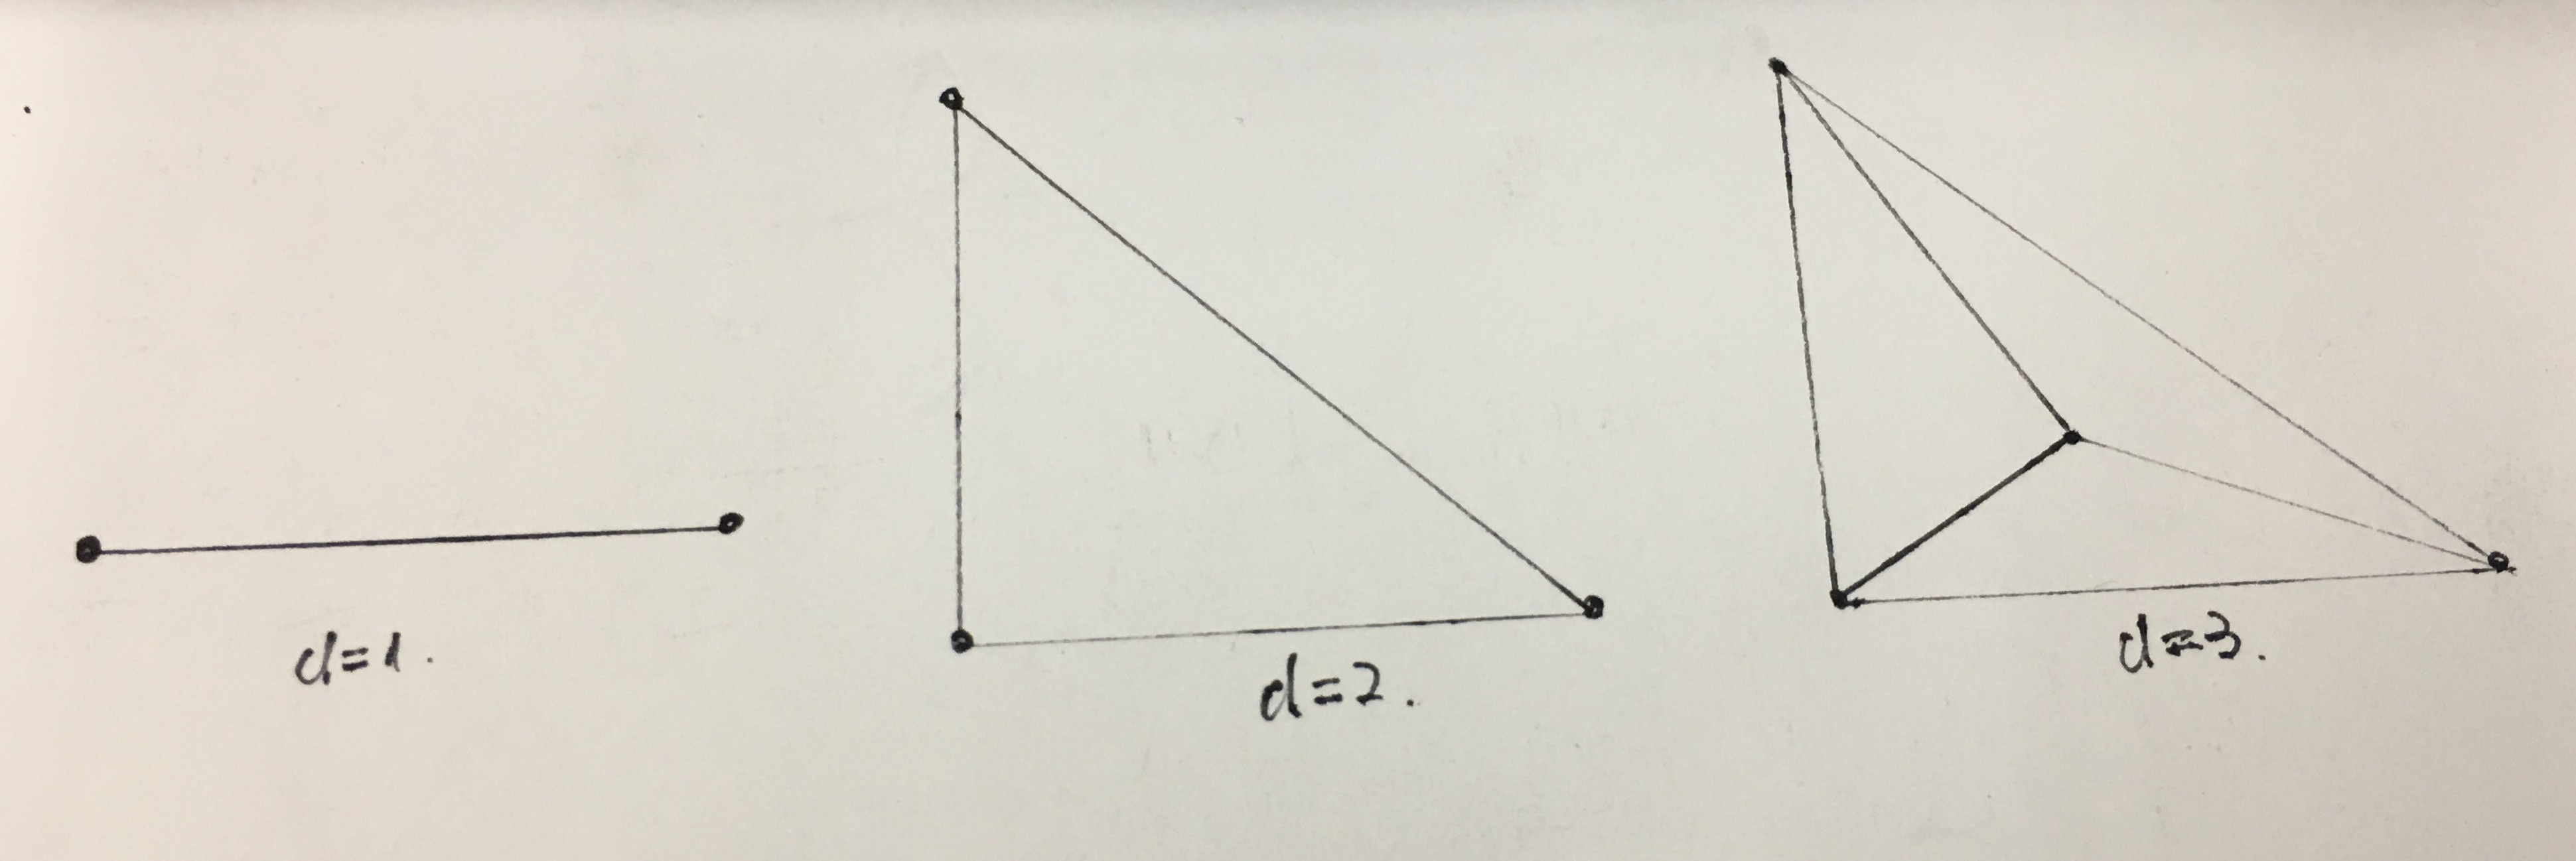
\includegraphics[width=4in]{./figures/20171209-finele-nodes}
 \caption{有限元$\tau_{\ell}$及其结点$x_{k}$}
\label{fig:finele-ref-element-nodes}

%  \small{注:实线表示名义资金流动。虚线表示实际物质流动。}
\end{figure}

定义以下三个集合
\begin{itemize}
  \item $I(k)$表示全部网格$\tau_{\ell}$的集合
  \begin{equation*}
    I(k) \coloneqq \left\{ \ell \in \mathbb{N}: x_{k} \in \overline{\tau}_{\ell} \right\}, \quad k = 1, \ldots, M,
  \end{equation*}
  \item $J(\ell)$表示网格$\overline{\tau}_{\ell}$中全部结点$x_{k}$的集合
  \begin{equation*}
    J(\ell) \coloneqq \left\{ k \in \mathbb{N}: x_{k} \in \overline{\tau}_{\ell} \right\}, \quad \ell = 1, \ldots, N,
  \end{equation*}
  可见$\dim J(\ell) = d+1$,
  \item $K(j)$表示网格$\overline{\tau}_{\ell}$中全部边$k_{j}$的集合
  \begin{equation*}
    K(j) \coloneqq \left\{ \ell \in \mathbb{N} : k_{j} \in \overline{\tau}_{\ell} \right\}, \quad j = 1, \ldots, K.
  \end{equation*}
\end{itemize}

如果有限元分解\eqref{eq:finele-ref-decomposition}中,所有两个相邻元之间都有共享的结点(d=1,2,3),边(d=2,3),三角形(d=3),那么我们称这种分解为容许分解(admissible decomposition)\index{decomposition!admissible \dotfill 容许分解}。以$d=2$为例,容许和不容许分解的例子见图\ref{fig:finele-ref-decomp-admissible-example}。
\begin{figure}[htbp]
  \centering
  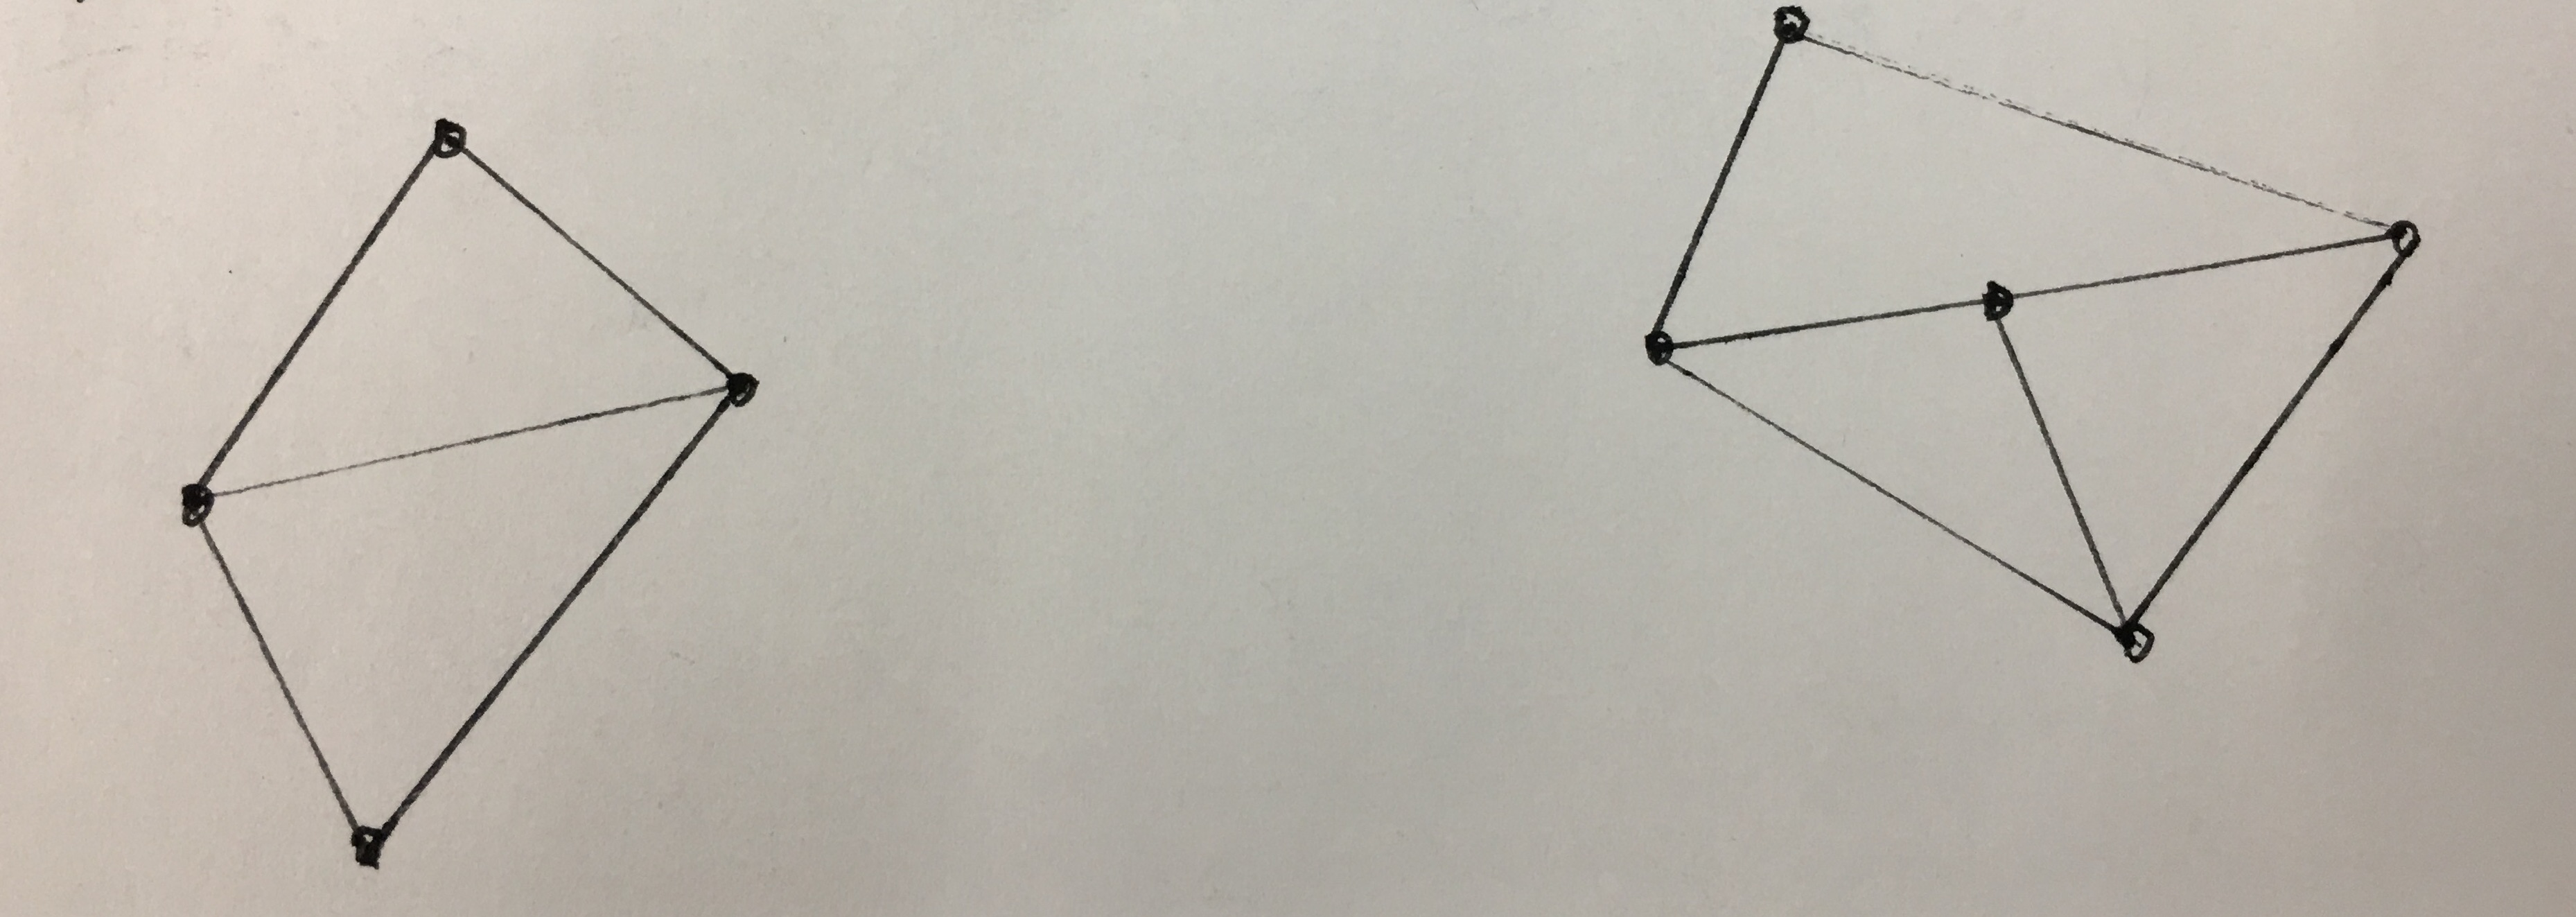
\includegraphics[width=4in]{./figures/20171209-decompo-adm-inadm.jpg}
 \caption{容许分解,以及不容许分解的三角分解($d=2$)}
\label{fig:finele-ref-decomp-admissible-example}

%  \small{注:实线表示名义资金流动。虚线表示实际物质流动。}
\end{figure}

在这里我们只考虑可计算域$\Omega$中容许分解的情况。对于某一有限元$\tau_{\ell}$,作如下定义
\begin{itemize}
  \item $\Delta_{\ell}$表示体积(volume)
  \begin{equation*}
    \Delta_{\ell} \coloneqq \int_{\tau_{\ell}} dx,
  \end{equation*}
  \item $h_{\ell}$表示局部网格尺寸(local mesh size)\index{mesh size!local \dotfill 局部网格尺寸}
  \begin{equation*}
    h_{\ell} \coloneqq \Delta_{\ell}^{\frac{1}{d}},
  \end{equation*}
  \item $d_{\ell}$表示(最大)直径,即有限元$\tau_{\ell}$中最长的一条边的长度
  \begin{equation*}
    d_{\ell} \coloneqq \sup_{x,y \in \tau_{\ell}}
    \left| x - y \right|,
  \end{equation*}
  显然对于$d=1$,我们有$\Delta_{\ell} = h_{\ell} = d_{\ell}$,
  \item 对应$d_{\ell}$,$r_{\ell}$表示(可包住)有限元$\tau_{\ell}$的最大圆($d=2$)或球体($d=3$)的半径。
\end{itemize}

经容许分解\eqref{eq:finele-ref-decomposition}后得到的有限元$\tau_{\ell}$,如果直径$d_{\ell}$由半径$r_{\ell}$约束而一致有界(uniformly bounded),即满足
\begin{equation*}
  d_{\ell} \le c_{F} \, r_{\ell}, \quad \ell = 1,\ldots,N,
\end{equation*}
那么我们称$\tau_{\ell}$为正则型有限元(regular finite element)\index{finite element!regular \dotfill 正则型有限元},其中常数$c_{F}$与$\mathcal{T}_{N}$:
\begin{itemize}
  \item 对于$d=2$的情况
  \begin{equation*}
    \begin{split}
      &\pi r_{\ell}^{2} \le \Delta_{\ell} = h_{\ell}^{2} \le d_{\ell}^{2} \le c_{F}^{2} r_{\ell}^{2}, \\
      \hookrightarrow &\pi^{\frac{1}{2}} r_{\ell} \le h_{\ell} \le d_{\ell} \le c_{F} r_{\ell},
    \end{split}
  \end{equation*}
  \item 对于$d=3$的情况
  \begin{equation*}
    \begin{split}
      &\frac{4}{3} \pi r_{\ell}^{3} \le \Delta_{\ell} = h_{\ell}^{3} \le d_{\ell}^{3} = c_{F}^{3} r_{\ell}^{3}, \\
      \hookrightarrow & \left( \frac{4}{3} \pi \right)^{\frac{1}{3}}
      r_{\ell} \le h_{\ell} \le d_{\ell} \le c_{F} r_{\ell}.
    \end{split}
  \end{equation*}
\end{itemize}

我们将最大、最小的局部网格尺寸分别定义为$h_{\max},h_{\min}$
\begin{equation*}
  \begin{split}
    h_{\max} & \coloneqq \max_{\ell =1,\ldots,N} h_{\ell}, \\
    h_{\min} & \coloneqq \min_{\ell =1,\ldots,N} h_{\ell},
  \end{split}
\end{equation*}
对应地将全局网格尺寸(global mesh size)\index{mesh size!global \dotfill 全局网格尺寸}定义为
\begin{equation*}
  h = h_{\max}.
\end{equation*}

如果$h_{\max}$和$h_{\min}$的比值小于等于一个全常数$c_{G} \ge 0$,即以下比值有界
\begin{equation*}
  \frac{h_{\max}}{h_{\min}} \le c_{G},
\end{equation*}
那么我们称对应的分解$\mathcal{T}_{N}$是全局拟一致的(globally quasi-uniform)\index{quansi-uniform!globally \dotfill 全局拟一致}的;$c_{G} \ge 1$的值与$N \in \mathbb{N}$无关。

对应地,如果对于任何两个临近的有限元$\tau_{\ell}$和$\tau{j}$都有
\begin{equation*}
  \frac{h_{\ell}}{h_{j}} \le c_{L}, \ell,j = 1,\ldots,N,
\end{equation*}
那么我们称这样的分解$\mathcal{T}_{N}$为局部拟一致(locally quasi-uniform)\index{quasi-uniform!locally \dotfill 局部拟一致}。
对于某一组相邻的有限元$\overline{\tau}_{\ell}$和$\overline{\tau}_{j}$,如果$\overline{\tau}_{\ell} \cap \overline{\tau}_{j}$包括不少于1个结点、1条边或1个三角形,那么我们称二者为相邻有限元(neighboring)\index{finite element!neighboring \dotfill 相邻有限元}。

\subsubsection{一维空间的局部参数化}
$d=1$时,每个有限元$\tau_{\ell}$都可以用局部参数化(local parameterization)\index{parameterization!local \dotfill 局部参数化}的形式予以描述。尤其是对于$x \in \tau_{\ell}, \, \ell_{1}, \ell_{2} \in J(\ell)$,我们有
\begin{equation*}
  x = x_{\ell_{1}} + \xi \left( x_{\ell_{2}} - x_{\ell_{1}} \right)
  =x_{\ell_{1}} + \xi h_{\ell}, \quad \xi \in (0,1),
\end{equation*}
其中我们将$\tau \coloneqq (0,1)$称为参考元(reference element)\index{reference element \dotfill 参考元}。

考虑这样一个方程$\nu(x), \, x \in \tau_{\ell}$,由上面的定义可得
\begin{equation*}
  \nu(x) = \nu(x_{\ell_{1}} + \xi h_{\ell} ) \eqqcolon \widetilde{\nu}_{\ell}(\xi), \quad \forall \, \xi \in \tau,
\end{equation*}
即对于$x \in \tau_{\ell}$,我们可以将方程$\nu(x)$识别为参考元中的方程$\widetilde{\nu}_{\ell}(\xi), \, \xi \in \tau$,对应范数

\begin{equation*}
  \begin{split}
    \left\| \nu \right\|_{L^{2}(\tau_{\ell})}^2
    &= \int_{\tau_{\ell}} \left( \nu(x) \right)^{2} \, dx = \int_{\tau} \left| \widetilde{\nu}_{\ell}(\xi) \right|^{2} h_{\ell} \, d \xi \\
    & = h_{\ell} \left\| \widetilde{\nu}_{\ell}(\xi) \right\|_{L^{2}(\tau)}^{2}.
  \end{split}
\end{equation*}

我们经常需要计算识别方程的导数,根据链式法则\eqref{eq:chain-rule-exa}可得
\begin{enumerate}
  \item 一阶导数
  \begin{equation*}
    \begin{split}
      &\frac{d}{d \xi} \widetilde{\nu}_{\ell}(\xi) = h_{\ell} \frac{d}{d x} \nu(x), \\
      \hookrightarrow & \frac{d}{d x}\nu(x) =
      h_{\ell}^{-1} \frac{d}{d \xi} \widetilde{\nu}_{\ell}(\xi), \quad \, x \in \tau_{\ell}, \, \xi \in \tau.
    \end{split}
  \end{equation*}
  \item 推广至高阶导数如$m \in \mathbb{N}$的情况
  \begin{equation*}
    \begin{split}
      \frac{d^{m}}{d x^{m}} \nu(x) = h^{- m} \frac{d^{m}}{d \xi^{m}}
      \widetilde{\nu}_{\ell}(\xi), \quad \, x \in \tau_{\ell}, \, \xi \in \tau,
    \end{split}
  \end{equation*}
  对应局部范数
  \begin{equation}
    \label{eq:finele-ref-local-norm}
    \left\|
    \frac{d^{m}}{d x^{m}}  \nu
    \right\|_{L^{2}(\tau_{\ell})}^{2}
    = h_{\ell}^{1-2m}
    \left\|
    \frac{d^{m}}{d \xi^{m}} \widetilde{\nu}_{\ell}
    \right\|_{L^{2}(\tau)}^{2}, \quad m \in \mathbb{N}_{0}.
  \end{equation}
\end{enumerate}

\subsubsection{二维空间的局部参数化}
$d=2$时,有限元$\tau_{\ell}$和参考元$\tau$的关系,见图\ref{fig:finele-ref-finele-refele}。

\begin{figure}[htbp]
  \centering
  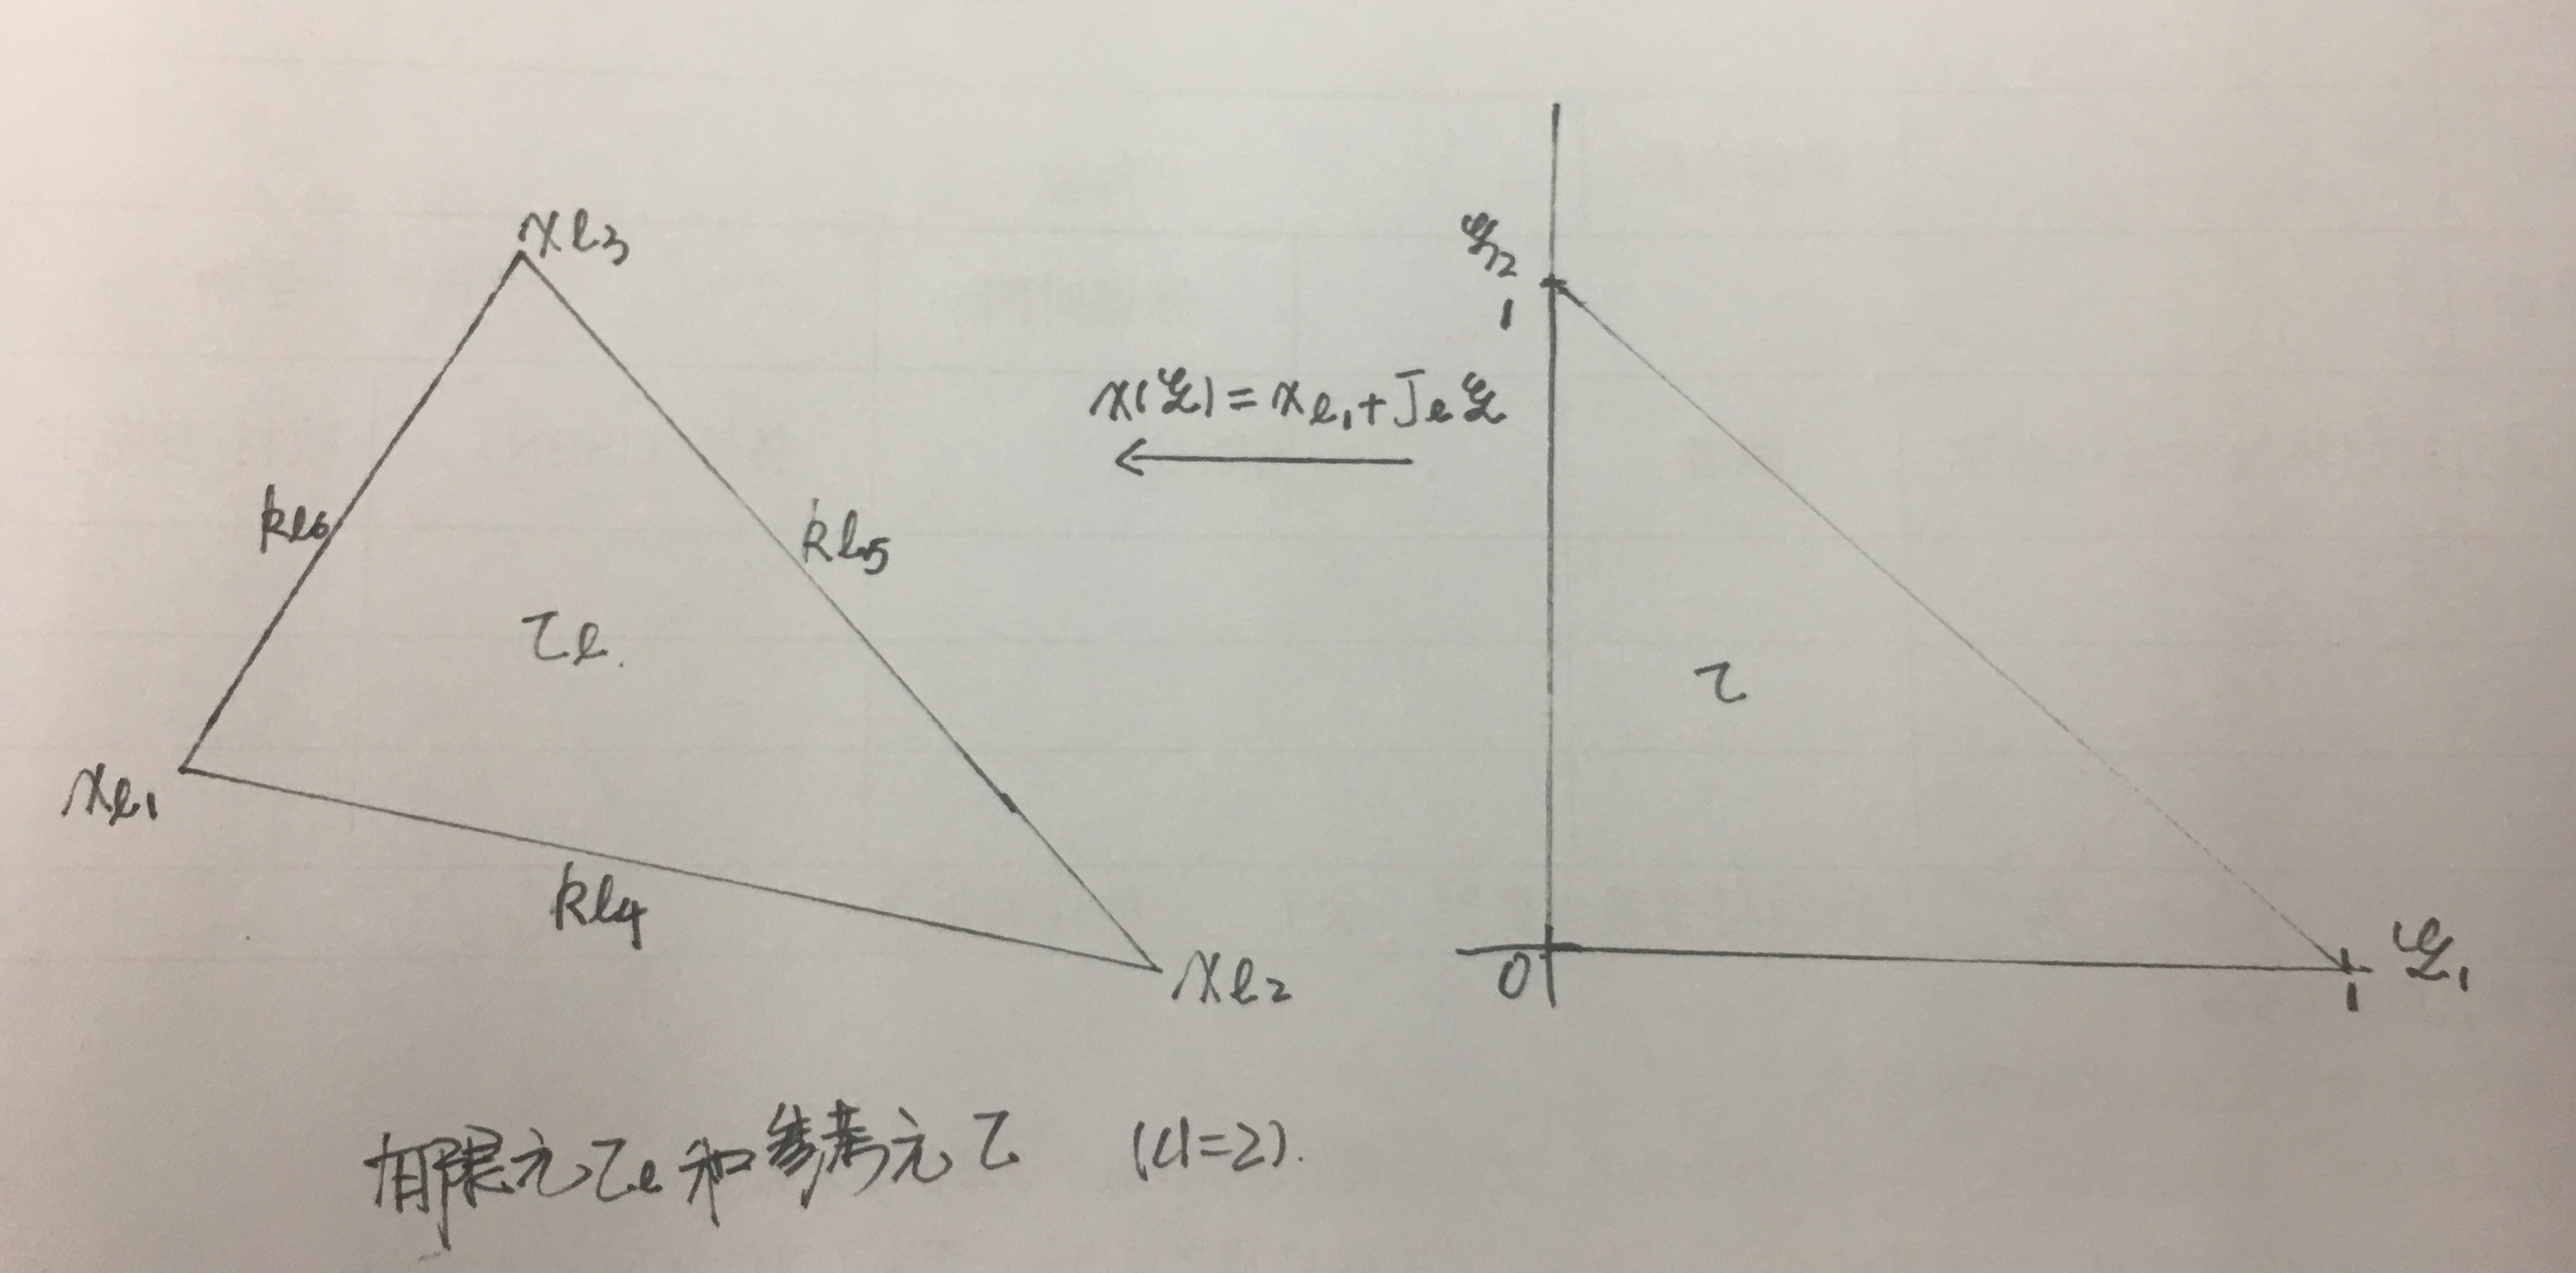
\includegraphics[width=4in]{./figures/20171210-finele-refele}
 \caption{有限元$\tau_{\ell}$和参考元$\tau$($d=2$)}
\label{fig:finele-ref-finele-refele}

%  \small{注:实线表示名义资金流动。虚线表示实际物质流动。}
\end{figure}

参考元$\tau$由下面三角形给出
\begin{equation}
  \label{eq:finele-ref-d2-refele-def}
  \tau = \left\{
  \xi \in \mathbb{R}^{2}: 0 \le \xi_{1} \le 1, \, 0 \le \xi_{2} \le 1 - \xi_{1} \right\}.
\end{equation}

对$x \in \tau_{\ell}$作局部参数化
\begin{equation*}
  x = x_{\ell_{1}} + \sum_{i=1}^{2} \xi_{i} \left( x_{\ell_{i+1}} - x_{\ell_{1}} \right) = x_{\ell_{1}} + J_{\ell} \, \xi, \quad \xi \in \tau,
\end{equation*}
其中$J_{\ell}$是个雅各比矩阵
\begin{equation*}
  J_{\ell} \coloneqq
  \begin{pmatrix}
    x_{\ell_{2}, 1} - x_{\ell_{1}, 1} &
    x_{\ell_{3}, 1} - x_{\ell_{1}, 1} \\
    x_{\ell_{2}, 2} - x_{\ell_{1}, 2} &
    x_{\ell_{3}, 2} - x_{\ell_{1}, 2}
  \end{pmatrix}.
\end{equation*}

由此我们得有限元$\tau_{\ell}$的面积,同时也是体积
\begin{equation*}
\begin{split}
    \Delta_{\ell} & = \int_{\tau_{\ell}} d s_{x} = \int_{\tau} \left| \det J_{\ell} \right| d \xi \\
    & = \left| \det J_{\ell} \right| \int_{0}^{1} \int_{0}^{1-\xi_{1}} d \xi_{2} d \xi_{1} = \frac{1}{2} \left| \det J_{\ell} \right|,
\end{split}
\end{equation*}
\begin{equation}
  \label{eq:finele-ref-d2-volume-matrix-determinant}
  \hookrightarrow \left| \det J_{\ell} \right| = 2 \Delta_{\ell}.
\end{equation}

$\nu(x), \, x \in \tau_{\ell}$对应的识别方程可表示为
\begin{equation*}
  \nu(x) = \nu \left( x_{\ell_{1}} + J_{\ell} \xi \right)
  \eqqcolon \widetilde{\nu}_{\ell}(\xi), \quad \xi \in \tau.
\end{equation*}

继续应用链式法则
\begin{equation*}
  \begin{split}
    & \triangledown_{\xi} \widetilde{\nu}_{\ell}(\xi) = J_{\ell}^{\top} \triangledown_{x} \nu(x), \\
    \hookrightarrow & \triangledown_{x} \nu(x) = J_{\ell}^{- \top} \triangledown_{\xi} \widetilde{\nu}_{\ell}(\xi).
\end{split}
\end{equation*}

等价范数的测度由下引理给出。
\begin{lemma}[识别方程等价范的测度($d=2$)]
  \label{lemma:finele-ref-d2-norm-equiv}
  $d=2, \, m \in \mathbb{N}_{0}$的情况下,识别方程的等价范满足不等式关系
  \begin{equation}
    \label{eq:finele-ref-d2-norm-equiv}
    \begin{split}
      \frac{1}{c_{m}} \left( 2 \Delta_{\ell} \right)^{1-m} \,
      \left\| \triangledown_{\xi}^{m}
      \widetilde{\nu}_{\ell}
      \right\|_{L^{2}(\tau)}^{2}
      \le \left\| \triangledown_{x}^{m} \nu \right\|_{L^{2}(\tau_{\ell})}^{2}
      \le c_{m} \, \left( 2 \Delta_{\ell} \right)^{1-m} \,
      \left\| \triangledown_{\xi}^{m} \widetilde{\nu}_{\ell}
      \right\|_{L^{2}(\tau)}^{2},
    \end{split}
  \end{equation}
  其中常数$c_{m} = \left( \frac{c_{F}^{2}}{\pi} \right)^{m}$。
\end{lemma}

\begin{proof}
  对于$m \in \mathbb{N}_{0}$,分三种情况来分别证明。
\begin{enumerate}
  \item $m=0$时。
  \begin{equation*}
    \begin{split}
      \left\| \nu \right\|_{L^{2}(\tau_{\ell})}^{2}
      &= \int_{\tau_{\ell}} \left| \nu(x) \right|^{2} \, dx \\
      & = \int_{\tau} \left| \widetilde{\nu}_{\ell} (\xi) \right|^{2}
      \left| \det J_{\ell} \right| \, d \xi \\
      & = 2 \Delta_{\ell} \, \left\| \widetilde{\nu}_{\ell} (\xi) \right\|_{L^{2}(\tau)}^{2},
    \end{split}
  \end{equation*}
  可证得\eqref{eq:finele-ref-d2-norm-equiv}成立。

  \item $m=1$时。
  \begin{equation*}
    \begin{split}
      \left\| \triangledown_{x} \nu \right\|_{L^{2}(\tau_{\ell})}^2
      & = \int_{\tau_{\ell}} \left| \triangledown_{x} \nu(x) \right|^{2} \, dx \\
      & = \int_{\tau}
      \left| J_{\ell}^{- \top} \triangledown_{\xi} \widetilde{\nu}_{\ell} (\xi) \right|^{2} \,
      \left| \det J_{\ell} \right|
      \, d \xi\\
      & = 2 \Delta_{\ell} \int_{\tau}
      \left(
      J_{\ell}^{-\top} \triangledown_{\xi} \widetilde{\nu}_{\ell} (\xi),
      \triangledown_{\xi} \widetilde{\nu}_{\ell} (\xi)
      \right) \,
      d \xi \\
      & = 2 \Delta_{\ell} \int_{\tau}
      \left(
      J_{\ell}^{-1} J_{\ell}^{-\top} \triangledown_{\xi} \widetilde{\nu}_{\ell} (\xi),
      \triangledown_{\xi} \widetilde{\nu}_{\ell} (\xi)
      \right) \, d \xi \\
      & \le 2 \Delta_{\ell} \lambda_{\max} \left(J_{\ell}^{-1} J_{\ell}^{-\top} \right) \,
      \int_{\tau}
      \left|
      \triangledown_{\xi} \widetilde{\nu}_{\ell} (\xi)
      \right| \, d_{\xi} \\
      & = 2 \Delta_{\ell} \lambda_{\max} \left(J_{\ell}^{-1} J_{\ell}^{-\top} \right) \,
      \left\|
      \triangledown_{\xi} \widetilde{\nu}_{\ell} (\xi)
      \right\|_{L^{2}(\tau)}^{2},
    \end{split}
  \end{equation*}

  以及类似地
  \begin{equation*}
    \begin{split}
      \left\| \triangledown_{x} \nu \right\|_{L^{2}(\tau_{\ell})}^2
      \ge 2 \Delta_{\ell} \, \lambda_{\min} \left(J_{\ell}^{-1} J_{\ell}^{-\top} \right) \,
      \left\|
      \triangledown_{\xi} \widetilde{\nu}_{\ell} (\xi)
      \right\|_{L^{2}(\tau)}^{2}.
    \end{split}
  \end{equation*}

  以上两个不等式都需要计算矩阵$\left(J_{\ell}^{-1} J_{\ell}^{-\top} \right)$的特征值,这可以从$\left(J_{\ell}^{\top} J_{\ell} \right)$开始
  \begin{equation*}
    J_{\ell}^{\top} J_{\ell} =
    \begin{pmatrix}
      a^{2} & a b \cos \alpha \\
      a b \cos \alpha & b^{2}
    \end{pmatrix},
  \end{equation*}
  其中
\begin{equation*}
  \begin{split}
    a & \coloneqq \left| x_{\ell_{2}} - x_{\ell_{1}} \right|, \\
    b & \coloneqq \left| x_{\ell_{3}} - x_{\ell_{1}} \right|, \\
    \alpha  & \coloneqq \sphericalangle
    \left( x_{\ell_{3}} - x_{\ell_{1}}, x_{\ell_{2}} - x_{\ell_{1}} \right).
  \end{split}
\end{equation*}

$\left(J_{\ell}^{-1} J_{\ell}^{-\top} \right)$的特征值为\footnote{善用Mathematica!}
\begin{equation*}
  \lambda_{1,2} = \frac{1}{2}
  \left[
  a^{2} + b^{2} \pm
  \left(
  \left(a^{2} - b^{2} \right)^2
  + 4 a^{2} b^{2} \left( \cos \alpha \right)^{2}
  \right)^{\frac{1}{2}}
  \right]
\end{equation*}
\begin{itemize}
  \item 对应的上限特征值$\lambda_{1}$有
  \begin{equation*}
    \frac{1}{2} \left( a^{2} + b^{2} \right) \le \lambda_{1} \le a^{2} + b^{2},
  \end{equation*}
  \item 两个特征值的乘积,根据\eqref{eq:finele-ref-d2-volume-matrix-determinant}有
  \begin{equation*}
    \lambda_{1} \lambda_{2} = \det \left| J_{\ell}^{\top} J_{\ell} \right|
    = \det \left| J_{\ell} \right|^{2}
    = 4 \Delta_{\ell}^{2}.
  \end{equation*}
  \item 因此对应的下限特征值$\lambda_{2}$有
  \begin{equation*}
    \lambda_{2} = \frac{4 \Delta_{\ell}^{2}}{\lambda_{1}} \ge \frac{4 \Delta_{\ell}^{2}}{a^{2} + b^{2}}.
  \end{equation*}
  \item 由此我们有
  \begin{equation*}
    \frac{4 \Delta_{\ell}^{2}}{a^{2} + b^{2}}
    \le \lambda_{\min}\left( J_{\ell}^{\top} J_{\ell} \right)
    \le \lambda_{\max}\left( J_{\ell}^{\top} J_{\ell} \right)
    \le a^{2} + b^{2}.
  \end{equation*}
  \item 此外根据定义我们有
  \begin{equation*}
    a^{2} + b^{2} \le 2 d_{\ell}^{2} \le 2 c_{F}^{2} r_{\ell}^{2}
    \le \frac{2 c_{F}^{2}}{\pi} \Delta_{\ell},
  \end{equation*}
  代入上式,整理得
  \begin{equation*}
    \frac{2 \pi}{c_{F}^{2}} \Delta_{\ell}
    \le \lambda_{\min} \left( J_{\ell}^{\top} J_{\ell} \right)
    \le \lambda_{\max}\left( J_{\ell}^{\top} J_{\ell} \right)
    \le \frac{2 c_{F}^{2}}{\pi} \Delta_{\ell}.
  \end{equation*}
\end{itemize}

所以,$J_{\ell}^{\top} J_{\ell}$的逆矩阵$J_{\ell}^{-1} J_{\ell}^{-\top}$的特征值满足
\begin{equation*}
  \begin{split}
    &\frac{\pi}{c_{F}^{2}} \left( 2 \Delta_{\ell} \right)^{-1}
    \le \lambda_{\min} \left( J_{\ell}^{-1} J_{\ell}^{-\top} \right)
    \le \lambda_{\max} \left( J_{\ell}^{-1} J_{\ell}^{-\top} \right)
    \le \frac{c_{F}^{2}}{\pi} \left( 2 \Delta_{\ell} \right)^{-1}, \\
    \hookrightarrow &
    \left( \frac{1}{c_{m}} \right) \left( 2 \Delta_{\ell} \right)^{-1}  \left( 2 \Delta_{\ell} \right)^{-1}
    \le \lambda_{\min} \left( J_{\ell}^{-1} J_{\ell}^{-\top} \right)
    \le \lambda_{\max} \left( J_{\ell}^{-1} J_{\ell}^{-\top} \right)
    \le c_{m} \left( 2 \Delta_{\ell} \right)^{-1},
  \end{split}
\end{equation*}
因此证得\eqref{eq:finele-ref-d2-norm-equiv}。

\item $m>1$时,可通过递归重复上述步骤证得\eqref{eq:finele-ref-d2-norm-equiv}。
\end{enumerate}
\end{proof}

\subsubsection{三维空间的局部参数化}
$d=3$时,参考元$\tau$表现为四面体(tetraderon)形式
\begin{equation*}
  \begin{split}
    \tau = \left\{
    \xi \in \mathbb{R}^{3} :
    0 \le \xi_{1} \le 1, \,
    0 \le \xi_{2} \le 1 - \xi_{1}, \,
    0 \le \xi_{3} \le 1 - \xi_{1} - \xi_{2}
    \right\}.
  \end{split}
\end{equation*}

对$x \in \tau_{\ell}$作局部参数化
\begin{equation*}
  x = x_{\ell_{1}} + \sum_{i=1}^{3} \xi_{1} \left( x_{\ell_{i+1}} - x_{\ell_{1}} \right)
  = x_{\ell_{1}} + J_{\ell} \xi, \quad \, \xi \in \tau,
\end{equation*}
其中雅各比矩阵
\begin{equation*}
  J_{\ell} =
  \begin{pmatrix}
    x_{\ell_{2},1} - x_{\ell_{1},1} &
    x_{\ell_{3},1} - x_{\ell_{1},1} &
    x_{\ell_{4},1} - x_{\ell_{1},1} \\
    x_{\ell_{2},2} - x_{\ell_{1},2} &
    x_{\ell_{3},2} - x_{\ell_{1},2} &
    x_{\ell_{4},2} - x_{\ell_{1},2} \\
    x_{\ell_{2},3} - x_{\ell_{1},3} &
    x_{\ell_{3},3} - x_{\ell_{1},3} &
    x_{\ell_{4},3} - x_{\ell_{1},3}
  \end{pmatrix}.
\end{equation*}

有限元的体积
\begin{equation*}
  \begin{split}
  \Delta_{\ell} & = \int_{\tau_{\ell}} d s_{x}
  = \int_{\tau} \left| \det J_{\ell} \right| d \xi \\
  & = \left| \det J_{\ell} \right| \,
  \int_{0}^{1} \int_{0}^{1 - \xi_{1}} \int_{0}^{1 - \xi_{1} - \xi_{2}} \, d \xi_{3} \, d \xi_{2} \, d \xi_{1} \\
  & = \frac{1}{6} \left| \det J_{\ell} \right|,
\end{split}
\end{equation*}
\begin{equation}
  \label{eq:finele-ref-d3-volume-matrix-determinant}
  \hookrightarrow \left| \det J_{\ell} \right| = 6 \Delta_{\ell}.
\end{equation}

用识别方程$\widetilde{\nu}_{\ell}(\xi), \, \xi \in \tau$来识别$\nu(x), \, x \in \tau_{\ell}$
\begin{equation*}
  \nu(x) = \nu \left( x_{\ell_{1}} + J_{\ell} \xi \right)
  \eqqcolon \widetilde{\nu}_{\ell}(\xi), \quad \xi \in \tau.
\end{equation*}

根据链式法则,可得导数
\begin{equation*}
  \begin{split}
    & \triangledown_{\xi} \widetilde{\nu}_{\ell} (\xi) = J_{\ell}^{\top} \triangledown_{x} \nu(x), \\
    & \hookrightarrow \triangledown_{x} \nu(x) = J_{\ell}^{\top} \triangledown_{\xi} \widetilde{\nu}_{\ell} (\xi).
  \end{split}
\end{equation*}

等价范数的测度见下引理。
\begin{lemma}[识别方程等价范的测度(d=3)]
  \label{lemma:finele-ref-d3-norm-equiv}
  $d=3,\,m\in \mathbb{N}_{0}$的情况下,识别方程的等价范满足不等式关系
  \begin{equation}
    \label{eq:finele-ref-d3-norm-equiv}
    c_{1} \Delta_{\ell} h_{\ell}^{- 2 m} \,
    \left\|
    \triangledown_{\xi}^{m} \widetilde{\nu}_{\ell}
    \right\|_{L^{2}(\tau)}^{2}
    \le \left\| \triangledown_{x}^{m} \nu
    \right\|_{L^{2}(\tau_{\ell})}^{2}
    \le c_{2} \Delta_{\ell} h_{\ell}^{- 2 m}
    \left\|
    \triangledown_{\xi}^{m} \widetilde{\nu}_{\ell}
    \right\|_{L^{2}(\tau)}^{2}
  \end{equation}
  其中常数$(c_{1}, c_{2}) > 0$,可能与$m$和$c_{F}$有关。
\end{lemma}
\begin{proof}
  分三种情况来证明。
\begin{enumerate}
  \item $m=0$时。
  \begin{equation*}
    \begin{split}
      \left\| \nu(x) \right\|_{L^{2}(\tau_{\ell})}^{2}
      & = \int_{\tau_{\ell}} \left| \nu(x) \right|^{2} \, d x \\
      & = \int_{\tau}
      \left| \widetilde{\nu}_{\ell}(\xi) \right|^{2} \,
      \left| \det J_{\ell} \right|
      \, d \xi \\
      & = 6 \Delta_{\ell}
      \left\| \widetilde{\nu}_{\ell}(\xi) \right\|_{L^{2}(\tau)},
    \end{split}
  \end{equation*}
可证得\eqref{eq:finele-ref-d3-norm-equiv}成立。

\item $m=1$时。
\begin{equation*}
  \begin{split}
    \left\|
    \triangledown_{x} \nu
    \right\|_{L^{2}(\tau_{\ell})}^{2}
    & = \int_{\tau_{\ell}}
    \left| \triangledown_{x} \nu(x) \right|^{2}
    \, dx \\
    & = \int_{\tau}
    \left| \det J_{\ell} \right| \,
    \left|
    J_{\ell}^{-\top} \triangledown_{\xi} \widetilde{\nu}_{\ell} \left( \xi \right)
    \right|^{2}
    \, d \xi \\
    & = \left| \det J_{\ell} \right| \,
    \int_{\tau} \left(
    J_{\ell}^{-\top} \triangledown_{\xi} \widetilde{\nu}_{\ell} \left( \xi \right),
    J_{\ell} \triangledown_{\xi} \widetilde{\nu}_{\ell} \left( \xi \right)
    \right)
    \, d \xi \\
    & = 6 \Delta_{\ell}
    \int_{\tau} \left(
    J_{\ell}^{-1} J_{\ell}^{-\top} \triangledown_{\xi} \widetilde{\nu}_{\ell} \left( \xi \right),
    \triangledown_{\xi} \widetilde{\nu}_{\ell} \left( \xi \right)
    \right)
    \, d \xi
  \end{split}
\end{equation*}
\begin{equation*}
  \hookrightarrow \left\|
  \triangledown_{x} \nu
  \right\|_{L^{2}(\tau_{\ell})}^{2}
  \begin{cases}
    \ge 6 \Delta_{\ell} \lambda_{\min}
    \left(
    J_{\ell}^{-1} J_{\ell}^{-\top}
    \right) \,
    \left\|
    \triangledown_{\xi} \widetilde{\nu}_{\ell}
    \right\|_{L^{2}(\tau)}^{2}  \\
    \le 6 \Delta_{\ell} \lambda_{\max}
    \left(
    J_{\ell}^{-1} J_{\ell}^{-\top}
    \right) \,
    \left\|
    \triangledown_{\xi} \widetilde{\nu}_{\ell}
    \right\|_{L^{2}(\tau)}^{2}
  \end{cases}
\end{equation*}

计算$\left( J_{\ell}^{\top} J_{\ell} \right)$矩阵的特征值
\begin{equation*}
  J_{\ell}^{\top} J_{\ell} =
  \begin{pmatrix}
    a^{2} & a b \cos \alpha & a c \cos \beta \\
    a b \cos \alpha & b^{2} & b c \cos \gamma \\
    a c \cos \beta & b c \cos \gamma & c^{2}
  \end{pmatrix},
\end{equation*}
其中
\begin{equation*}
  \begin{split}
    a & \coloneqq \left| x_{\ell_{2}} - x_{\ell_{1}} \right|, \\
    b & \coloneqq \left| x_{\ell_{3}} - x_{\ell_{1}} \right|, \\
    b & \coloneqq \left| x_{\ell_{4}} - x_{\ell_{1}} \right|, \\
    \alpha & \coloneqq \sphericalangle
    \left(
    x_{\ell_{2}} - x_{\ell_{1}},
    x_{\ell_{3}} - x_{\ell_{1}}
    \right), \\
    \beta & \coloneqq \sphericalangle
    \left(
    x_{\ell_{2}} - x_{\ell_{1}},
    x_{\ell_{4}} - x_{\ell_{1}}
    \right), \\
    \gamma & \coloneqq \sphericalangle
    \left(
    x_{\ell_{3}} - x_{\ell_{1}},
    x_{\ell_{4}} - x_{\ell_{1}}
    \right), \\
  \end{split}
\end{equation*}

对应的三个特征值$\lambda_{i} > 0, \, i = 1,2,3$,满足
\begin{equation*}
  \begin{split}
    \sum_{i=1}^{3} \lambda_{i} &= \trace \left( J_{\ell}^{\top} J_{\ell} \right) = a^{2} + b^{2} + c^{2}, \\
    \prod_{i=1}^{3} \lambda_{i} &= \det \left( J_{\ell}^{\top} J_{\ell} \right) = \left| \det J_{\ell} \right|^{2} = 36 \Delta_{\ell}
  \end{split}
\end{equation*}
\begin{itemize}
  \item 最大特征值的上限
  \begin{equation*}
    \lambda_{\max} \left( J_{\ell}^{\top} J_{\ell} \right) \le a^{2} + b^{2} + c^{2}.
  \end{equation*}
  \item 因此可得最小特征值的下限
  \begin{equation*}
    %\begin{split}
      \lambda_{\min} \left( J_{\ell}^{\top} J_{\ell} \right)
      \ge \frac{\prod_{i=1}^{3} \lambda_{i}}{\lambda_{\max}^{2} \left( J_{\ell}^{\top} J_{\ell} \right)}
      \ge \frac{
      36 \Delta_{\ell}^{2}
      }{
      \left( a^{2} + b^{2} + c^{2} \right)^{2}
      }
    %\end{split}
  \end{equation*}
  \item 因此我们有
  \begin{equation*}
    \frac{
    36 \Delta_{\ell}^{2}
    }{
    \left( a^{2} + b^{2} + c^{2} \right)^{2}
    }
    \le \lambda_{\min} \left( J_{\ell}^{\top} J_{\ell} \right)
    \le \lambda_{\max} \left( J_{\ell}^{\top} J_{\ell} \right)
    \le a^{2} + b^{2} + c^{2}.
  \end{equation*}
\end{itemize}

由于假定$\tau_{\ell}$是正则型有限元(regular shape)\index{finite element!regular \dotfill 正则型有限元},则所有边的长度对应
\begin{equation*}
  a^{2} + b^{2} + c^{2}
  \le 3 d_{\ell}^{2}
  \le 3 c_{F}^{2} r_{\ell}^{2}
  \le 3 \left( \frac{4}{3} \pi \right)^{-\frac{2}{3}}
  c_{F}^{2} h_{\ell}^{2}.
\end{equation*}

代入上式可得
\begin{equation*}
  \frac{4}{c_{F}^{4}}
  \left( \frac{4}{3} \pi \right)^{\frac{4}{3}}
  h_{\ell}^{2}
  \le \lambda_{\min} \left( J_{\ell}^{\top} J_{\ell} \right)
  \le \lambda_{\max} \left( J_{\ell}^{\top} J_{\ell} \right)
  \le 3 \left( \frac{4}{3} \pi \right)^{- \frac{2}{3}}
  c_{F}^{2} h_{\ell}^{2}.
\end{equation*}
可证得\eqref{eq:finele-ref-d3-norm-equiv}成立。

\item $m>1$时,可通过递归重复上述步骤证得\eqref{eq:finele-ref-d3-norm-equiv}。
\end{enumerate}
\end{proof}

\subsubsection{识别方程等价范的测度不等式}
综上,识别方程等价范的测度不等式,$d=1$时为\eqref{eq:finele-ref-local-norm},$d=2$时为Lemma \ref{lemma:finele-ref-d2-norm-equiv}式\eqref{eq:finele-ref-d2-norm-equiv},$d=3$时为Lemma \ref{lemma:finele-ref-d3-norm-equiv}式\eqref{eq:finele-ref-d3-norm-equiv}。那么可以得到如下定理

\begin{theorem}[识别方程等价范的测度不等式]
\label{theorem:finele-ref-d123-norm-equiv}
设一个正则型的容许分解$\mathcal{T}_{N}$中的有限元$\tau_{\ell} \subset \mathbb{R}^{d}$。如果$\nu$充分平滑,对于$m \in \mathbb{N}_{0}$我们有
\begin{equation*}
%  \begin{split}
    c_{1} \Delta_{\ell} h_{\ell}^{-2m} \, \left\|
    \triangledown_{\xi}^{m} \widetilde{\nu}_{\ell}
    \right\|_{L^{2}(\tau)}^{2}
    \le \left\| \triangledown_{x}^{m} \nu
    \right\|_{L^{2}(\tau_{\ell})}^{2}
    \le c_{2} \Delta_{\ell} h^{-2m} \,
    \left\| \triangledown_{x}^{m} \nu
    \right\|_{L^{2}(\tau_{\ell})}^{2},
%  \end{split}
\end{equation*}
其中常数$\left(c_{1}, c_{2} \right)>0$,并且可能与$m$和$c_{F}$有关。
\end{theorem}

%!TEX root = ../DSGEnotes.tex
\subsection{形式方程}
\label{sec:finele-form}
基于分解元$\mathcal{T}_{N}$\eqref{eq:finele-ref-decomposition},现在来分析检测空间(trial spaces)\index{trial space \dotfill 检测空间}。检测空间由分段多项式构成,这些多项式组成不同形式的基方程(base functions)\index{base function \dotfill 基方程}。基方程与全局自由度相关,不过更是在局部定义的:是针对有限元$\tau_{\ell}$,通过选取合适的形式方程(form function)\index{form function \dotfill 形式方程}而作局部定义。

考虑这样一个参考元$\tau$,它可以是一个区间($d=1$),三角形($d=2$)或是四面体($d=3$)。

\subsubsection{常数型形式方程}
最简单的形式方程可以是个常数
\begin{equation*}
  \psi_{1}^{0}(\xi) = 1, \quad \xi \in \tau,
\end{equation*}

对应地,如果有限元$\tau_{\ell}$中的某个方程$\nu_{h}(x), \, x \in \tau_{\ell}$是个常数,那么$\nu$的表现形式可写为
\begin{equation*}
  \nu_{h}(x) = \nu_{h} \left( x_{\ell_{1}} + J_{\ell} \xi \right)
  =\nu_{\ell} \, \psi_{1}^{0}(\xi), \quad x \in \tau_{\ell}, \, \xi \in \tau,
\end{equation*}
其中系数$\nu_{\ell}$反映$\nu_{h} \in \tau_{\ell}$在参考元$\tau$中对应的值。由此可得
\begin{equation}
  \label{eq:finele-form-constant-norm}
  \left\| \nu_{h} \right\|_{L^{2}(\tau_{\ell})}^{2} = \Delta_{\ell} \nu_{\ell}^{2}.
\end{equation}

\subsubsection{线性形式方程}
如果$\nu_{h}(x), \, x \in \tau_{\ell}$是个线性方程,那么$\nu_{h}$可由参考元$\tau$中结点的值$\widetilde{\nu}_{k}$所唯一决定
\begin{equation}
  \label{eq:finele-form-lin-nuh-nuk}
  \widetilde{\nu}_{h}\left( \xi \right)
  = \sum_{k=1}^{d+1} \widetilde{\nu}_{k} \psi_{k}^{1}\left( \xi \right), \quad \xi \in \tau,
\end{equation}
其中$\psi_{k}^{1}$的值如下
\begin{itemize}
  \item $d=1$时结点数$k=2$
  \begin{equation*}
    \begin{cases}
      \psi_{1}^{1} & \coloneqq 1 - \xi,\\
      \psi_{2}^{1} & \coloneqq \xi.
    \end{cases}
  \end{equation*}
  \item $d=2$时节点数$k=3$
  \begin{equation*}
    \begin{cases}
      \psi_{1}^{1} & \coloneqq 1 - \xi_{1} - \xi_{2}, \\
      \psi_{2}^{1} & \coloneqq \xi_{1}, \\
      \psi_{3}^{1} & \coloneqq \xi_{2}.
    \end{cases}
  \end{equation*}
  \item $d=3$时节点数$k=4$
  \begin{equation*}
    \begin{cases}
      \psi_{1}^{1} & \coloneqq 1 - \xi_{1} - \xi_{2} - \xi_{3}, \\
      \psi_{2}^{1} & \coloneqq \xi_{1}, \\
      \psi_{3}^{1} & \coloneqq \xi_{2}, \\
      \psi_{4}^{1} & \coloneqq \xi_{3}.
    \end{cases}
  \end{equation*}
\end{itemize}

这样一来我们有:设任意一个有限元$\tau_{\ell}$,对应结点$x_{\ell_{k}}, \, \ell_{k} \in J(\ell)$。$\tau_{\ell}$中的线性方程$\nu_{h}(x), \, x \in \tau_{\ell}$可以写为
\begin{equation}
  \label{eq:finele-form-lin-nuh-reprensentation}
  \nu_{h} \left( x \right)
  = \nu_{h} \left( x_{\ell_{1}} + J_{\ell} \xi \right)
  = \sum_{k=1}^{d+1} \nu_{\ell_{k}} \psi_{k}^{1} \left( \xi \right), \quad x \in \tau_{\ell}, \xi \in \tau.
\end{equation}

与常数形式方程的范数\eqref{eq:finele-form-constant-norm}类似,线性形式方程$\nu_{h}(x), \, x \in \tau_{\ell}$的范数$\left\| \nu_{h} \right\|_{L^{2}} \left(\tau_{\ell} \right)$也可以用结点的值$\nu_{\ell}(\xi), \, \xi \in \tau$来表示,见如下引理。
\begin{lemma}[线性形式方程的范数]
  \label{lemma:finele-form-lin-norm-def}
  设线性方程$\nu_{h}(x), \, x \in \tau_{\ell}$如\eqref{eq:finele-form-lin-nuh-reprensentation}所示。那么我们有范数不等式关系
  \begin{equation}
    \label{eq:finele-form-lin-norm-def}
    \frac{\Delta_{\ell}}{\left( d+1 \right) \left( d+2 \right)}
    \sum_{k=1}^{d+1} \nu_{\ell_{k}}^{2}
    \le \left\| \nu_{h} \right\|_{L^{2}(\tau_{\ell})}^{2}
    \le \frac{\Delta_{\ell}}{\left( d+1 \right)}
    \sum_{k=1}^{d+1} \nu_{\ell_{k}}^{2}
  \end{equation}
\end{lemma}
\begin{proof}
  线性方程$\nu_{h}(x) \in L^{2}(\tau_{\ell})$的范数
  \begin{equation*}
    \begin{split}
      \left\| \nu_{h} \right\|_{L^{2}(\tau_{\ell})}^{2}
      & = \langle \nu_{h}, \nu_{h} \rangle_{L^{2}(\tau_{\ell})} \\
      & = \sum_{i=1}^{d+1} \sum_{j=1}^{d+1} \nu_{i} \nu_{j}
      \int_{\tau} \psi_{i}\left( \xi \right) \psi_{j}\left( \xi \right) \left| \det J_{\ell} \right| \, d \xi \\
      & = \left( G_{\ell} \, \underline{\nu}^{\ell}, \underline{\nu}^{\ell} \right),
    \end{split}
  \end{equation*}
  其中$G_{\ell}$是局部质量矩阵(local mass matrix)\index{mass matrix!local \dotfill 局部质量矩阵}
  \begin{equation*}
    G_{\ell} = \frac{
    \Delta_{\ell}
    }{
    \left( d + 1 \right)\left( d + 2 \right)}
    \underbrace{
    \left(
    I_{d+1} + \underline{e}_{d+1} \underline{e}_{d+1}^{\top}
    \right)
    }_{\eqqcolon \mathcal{A}}
    , \quad \underline{e}_{d+1} = \underline{1} \in \mathbb{R}^{d+1}.
  \end{equation*}

提取$G_{\ell}$矩阵$\mathcal{A}$,计算特征值,Mathematica中代码如下
\begin{verbatim}
  d = 3 (*三维系统d=3。改为2或1,对应二维、一维系统*)
  ee = Table[1, d + 1, d + 1]
  et = Transpose[ee]
  ii = IdentityMatrix[d + 1]
  new = ii + ee*et
  Eigenvalues[new]
\end{verbatim}
可得$\lambda_{1}\left[ \mathcal{A} \right]=1, \, \lambda_{2}\left[ \mathcal{A} \right] = \ldots = \lambda_{d+1} \left[ \mathcal{A} \right] =1$。进而证得\eqref{eq:finele-form-lin-norm-def}。
\end{proof}

许多应用中需要将$\nu_{h}(x)$的斜率与$\nu_{h}(x)$自身关联起来,见下引理。
\begin{lemma}[方程范数与方程斜率的范数]
  \label{lemma:finele-form-norm-gradient}
  设线性方程$\nu_{h}$如\eqref{eq:finele-form-lin-nuh-reprensentation}所给定。则以下局部逆不等式关系成立
  \begin{equation}
    \label{eq:finele-form-norm-gradient}
    \left\| \triangledown_{x} \nu_{h} \right\|_{L^{2}(\tau_{\ell})}
    \le c_{I} h_{\ell}^{-1} \left\| \nu_{h} \right\|_{L^{2}(\tau_{\ell})},
  \end{equation}
  其中常数$c_{I} > 0$。
\end{lemma}
\begin{proof}
  分以下几步来证明。

  第一步。由Theorem \ref{theorem:finele-ref-d123-norm-equiv} 可得$\nu_{h}(x), \, x \in \tau_{\ell}$方程斜率的范,与形式方程$\widetilde{nu}_{\ell} (\xi), \, \xi \in \tau$方程斜率范的关系
\begin{equation*}
  \left\| \triangledown_{x} \nu_{h} \right\|_{L^{2}(\tau_{\ell})}^{2}
  \le c_{2} \Delta_{\ell} h_{\ell}^{-2} \,
  \left\| \triangledown_{\xi} \widetilde{\nu}_{\ell}
  \right\|_{L^{2}(\tau)}^{2}.
\end{equation*}

那么下面需要计算线性方程
\begin{equation*}
\widetilde{\nu}_{\ell} (\xi) = \sum_{k=1}^{d+1} \nu_{\ell_{k}} \psi_{k}^{1} \left( \xi \right)
\end{equation*}
的斜率以及范数。分$d=1,2,3$三种情况。
\begin{itemize}
  \item $d=1$时,
  \begin{equation*}
    \triangledown_{\xi} \widetilde{\nu}_{\ell} = \nu_{\ell_{2}} - \nu_{\ell_{1}},
  \end{equation*}
  \begin{equation*}
    \begin{split}
      \left\| \triangledown_{\xi} \widetilde{\nu} \right\|_{L^{2}(\tau_{\ell})}^{2}
      & = \left( \nu_{\ell_{2}} - \nu_{\ell_{2}} \right)^{2}
      \le 2 \left[
      \nu_{\ell_{2}}^{2} + \nu_{\ell_{1}}^{2}
      \right]
      \le 4 \left\| \nu_{h} \right\|_{L^{\infty}(\tau_{\ell})}^{2}.
    \end{split}
  \end{equation*}
  \item $d=2$时,
  \begin{equation*}
    \triangledown_{\xi} \widetilde{\nu}_{\ell} =
    \begin{pmatrix}
      \nu_{\ell_{2}} - \nu_{\ell_{1}} \\
      \nu_{\ell_{3}} - \nu_{\ell_{1}}
    \end{pmatrix},
  \end{equation*}
  \begin{equation*}
    \begin{split}
    \left\| \triangledown_{\xi} \widetilde{\nu}_{\ell} \right\|_{L^{2}(\tau)}^{2}
    & = \frac{1}{2} \,
    \left[
    \left( \nu_{\ell_{2}} - \nu_{\ell_{1}} \right)^{2} +
    \left( \nu_{\ell_{3}} - \nu_{\ell_{1}} \right)^{2}
    \right] \\
    & \le \frac{1}{2} \,
    \left[
    2 \nu_{\ell_{2}}^{2} + 2 \nu_{\ell_{3}}^{2} + 4 \nu_{\ell_{4}}^{2}
    \right] \\
    & \le 4 \, \left\| \nu_{h} \right\|_{L^{\infty}(\tau_{\ell})}.
  \end{split}
  \end{equation*}
  \item $d=3$时
  \begin{equation*}
    \triangledown_{\xi} \widetilde{\nu}_{\ell} =
    \begin{pmatrix}
      \nu_{\ell_{2}} - \nu_{\ell_{1}} \\
      \nu_{\ell_{3}} - \nu_{\ell_{1}} \\
      \nu_{\ell_{4}} - \nu_{\ell_{1}}
    \end{pmatrix},
  \end{equation*}
  \begin{equation*}
    \begin{split}
    \left\| \triangledown_{\xi} \widetilde{\nu}_{\ell} \right\|_{L^{2}(\tau)}^{2}
    & = \frac{1}{6} \,
    \left[
    \left( \nu_{\ell_{2}} - \nu_{\ell_{1}} \right)^{2} +
    \left( \nu_{\ell_{3}} - \nu_{\ell_{1}} \right)^{2} +
    \left( \nu_{\ell_{4}} - \nu_{\ell_{1}} \right)^{2}
    \right] \\
    & \le \frac{1}{6} \,
    \left[
    2 \nu_{\ell_{2}}^{2} + 2 \nu_{\ell_{3}}^{2} + 2 \nu_{\ell_{4}}^{2} + 6 \nu_{\ell_{1}}^{2}
    \right]\\
    & \le 4 \, \left\| \nu_{h} \right\|_{L^{\infty}(\tau_{\ell})}^{2}.
  \end{split}
  \end{equation*}
  \end{itemize}

汇总可得
  \begin{equation*}
    \begin{split}
      \left\| \triangledown_{x} \nu_{h} \right\|_{L^{2}(\tau_{\ell})}^{2}
      & \le c_{2} \Delta_{\ell} h_{\ell}^{-2} \,
      \left\| \triangledown_{\xi} \widetilde{\nu}_{\ell} \right\|_{L^{2}(\tau)}^{2} \\
      & \le 4 c_{2} \Delta_{\ell} h_{\ell}^{2} \left\| \nu_{h} \right\|_{L^{\infty}(\tau_{\ell})}^2,
    \end{split}
  \end{equation*}
\begin{equation*}
  \hookrightarrow \left\| \triangledown_{x} \nu_{h} \right\|_{L^{2}(\tau_{\ell})}
  \le c_{I} h_{\ell}^{-1} \,
  \left\| \nu_{h} \right\|_{L^{2}(\tau_{\ell})}.
\end{equation*}
\end{proof}

\subsubsection{二次形式方程}
更高幂次的非线性局部形式方程,可由相应的低幂次形式方程逐级地推定义而得。以二次形式方程为例,定义如下:
\begin{itemize}
  \item $d=1$时,
  \begin{equation*}
    \begin{cases}
      \psi_{1}^{2}(\xi) \coloneqq 1 - \xi, \\
      \psi_{2}^{2}(\xi) \coloneqq \xi, \\
      \psi_{3}^{2}(\xi) \coloneqq 4 \xi \left( 1 - \xi \right).
    \end{cases}
  \end{equation*}
  \item $d=2$时,
  \begin{equation*}
    \begin{cases}
      \psi_{1}^{2}(\xi) \coloneqq 1 - \xi_{1} - \xi_{2}, \\
      \psi_{2}^{2}(\xi) \coloneqq \xi_{1}, \\
      \psi_{3}^{2}(\xi) \coloneqq \xi_{2}, \\
      \psi_{4}^{2}(\xi) \coloneqq 4 \xi_{1} \left( 1 - \xi_{1} - \xi_{2} \right), \\
      \psi_{5}^{2}(\xi) \coloneqq 4 \xi_{1} \xi_{2}, \\
      \psi_{6}^{2}(\xi) \coloneqq 4 \xi_{2} \left( 1 - \xi_{1} - \xi_{2} \right).
    \end{cases}
  \end{equation*}
  \item $d=3$时,
  \begin{equation*}
    \begin{cases}
      \psi_{1}^{2}(\xi) \coloneqq 1 - \xi_{1} - \xi_{2} - \xi_{3}, \\
      \psi_{2}^{2}(\xi) \coloneqq \xi_{1}, \\
      \psi_{3}^{2}(\xi) \coloneqq \xi_{2}, \\
      \psi_{4}^{2}(\xi) \coloneqq \xi_{3}, \\
      \psi_{5}^{2}(\xi) \coloneqq 4 \xi_{1} \left( 1 - \xi_{1} - \xi_{2} - \xi_{3} \right), \\
      \psi_{6}^{2}(\xi) \coloneqq 4 \xi_{1} \xi_{2}, \\
      \psi_{7}^{2}(\xi) \coloneqq 4 \xi_{2} \left( 1 - \xi_{1} - \xi_{2} - \xi_{3} \right), \\
      \psi_{8}^{2}(\xi) \coloneqq 4 \xi_{3} \left( 1 - \xi_{1} - \xi_{2} - \xi_{3} \right), \\
      \psi_{9}^{2}(\xi) \coloneqq 4 \xi_{3} \xi_{1}, \\
      \psi_{10}^{2}(\xi) \coloneqq 4 \xi_{2} \xi_{3}.
    \end{cases}
  \end{equation*}
\end{itemize}

注意,线性形式方程与结点$x_{k} \in \overline{\tau}_{\ell}$的自由度有关,而非线性形式方程则与边的中值点$x_{k_{j}}^{*}$有关。若方程$x_{h}$在$\tau_{\ell}$中是二次形式的,那么可以写作
\begin{equation}
  \label{eq:finele-form-quadratic}
  \begin{split}
    \nu_{h}(x)
    & = \nu_{h} \left( x_{\ell_{1}} + J_{\ell} \xi \right) \\
    & = \sum_{k=1}^{\frac{1}{2} \left( d+1 \right)\left( d+2 \right)}
    \nu_{\ell_{k}} \psi_{k}^{2}(\xi), \quad \, x \in \tau_{\ell}, \, \xi \in \tau.
  \end{split}
\end{equation}

类似于Lemma \ref{lemma:finele-form-lin-norm-def},二次形式方程的范数可写作
\begin{equation*}
  \begin{split}
  \left\| \nu_{h} \right\|_{L^{2}(\tau_{\ell})}^{2}
  & = \sum_{i,j=1}^{\frac{1}{2} \left( d+1 \right) \left( d+2 \right)}
  \nu_{i} \nu_{j}
  \int_{\tau} \psi_{i}^{2}(\xi) \psi_{j}^{2}(\xi) \, \left| \det J_{\ell} \right| \, d \xi \\
  & = \left( G_{\ell} \underline{\nu}^{\ell}, \underline{\nu}^{\ell} \right),
\end{split}
\end{equation*}
\begin{itemize}
  \item $d=1$时,局部质量矩阵$G_{\ell}$为
  \begin{equation*}
    G_{\ell} =
    \begin{pmatrix}
      \frac{1}{3} & \frac{1}{6} & \frac{1}{3} \\
      \frac{1}{6} & \frac{1}{3} & \frac{1}{3} \\
      \frac{1}{3} & \frac{1}{3} & \frac{8}{15}
    \end{pmatrix},
  \end{equation*}
  对应特征值计算得
  \begin{equation*}
    \begin{split}
      \lambda_{1} &= \frac{\Delta_{\ell}}{6}, \\
      \lambda_{2} &= \Delta_{\ell} \left[ \frac{31}{60} + \frac{\sqrt{89}}{20} \right] \\
      \lambda_{2} &= \Delta_{\ell} \left[ \frac{31}{60} + \frac{\sqrt{89}}{20} \right].
    \end{split}
  \end{equation*}
  \item $d=2,3$时,
  \begin{itemize}
    \item 等价范数的估计与线性形式方程情况下的Lemma \ref{lemma:finele-form-lin-norm-def}式\eqref{eq:finele-form-lin-norm-def}一致
    \begin{equation}
      \label{eq:finele-form-quadratic-norm-def}
      c_{1} \Delta_{\ell} \sum_{k=1}^{\frac{1}{2}\left( d+1 \right)\left( d+2 \right)}
      \nu_{\ell_{k}}^{2}
      \le \left\| \nu_{h} \right\|_{L^{2}(\tau_{\ell})}^{2}
      \le c_{2} \Delta_{\ell} \sum_{k=1}^{\frac{1}{2}\left( d+1 \right)\left( d+2 \right)}
      \nu_{\ell_{k}}^{2},
    \end{equation}
    其中二次形式方程$\nu_{h}$的定义如\eqref{eq:finele-form-quadratic}。
    \item 逆不等式也与线性形式下的情况Lemma \ref{lemma:finele-form-norm-gradient}式\eqref{eq:finele-form-norm-gradient}相一致。
  \end{itemize}
\end{itemize}


\subsection{检测空间}
\label{sec:finele-trial}
对于二阶偏微分方程的边界值问题,为了计算近似解,需要我们构建检测空间$\mathcal{S}_{h}^{1}\left(\mathcal{T}_{N} \right)$,空间中包括局部分段线性方程和全局连续方程。

对于容许分解\eqref{eq:finele-ref-decomposition}来说,在分解产生的结点$x_{k}$处,$\mathcal{S}_{h}^{1}\left(\mathcal{T}_{N} \right)$便由结块方程(nodal function)所唯一确定,$\nu_{k} = \nu_{h}(x_{k})$。通过这样的方式,可以将有限元$\tau_{\ell}$用局部形式方程予以表现。

全局检测空间$\mathcal{S}_{h}^{1}\left(\mathcal{T}_{N} \right)$的维数$\dimm \mathcal{S}_{h}^{1}\left(\mathcal{T}_{N} \right)$也因此等于分解后的结点数。对应地,$\mathcal{S}_{h}^{1}\left(\mathcal{T}_{N} \right)$的基$\psi_{k}^{1}(x)$如图所示,可以写为
\begin{equation*}
  \psi_{k}^{1} (x) \coloneqq
  \begin{cases}
  1 & x = x_{k}, \\
  0 & x = x_{\ell} \neq x_{k}, \\
  \text{线性} & \text{其他情况}.
\end{cases}
\end{equation*}

\begin{figure}[htbp]
  \centering
  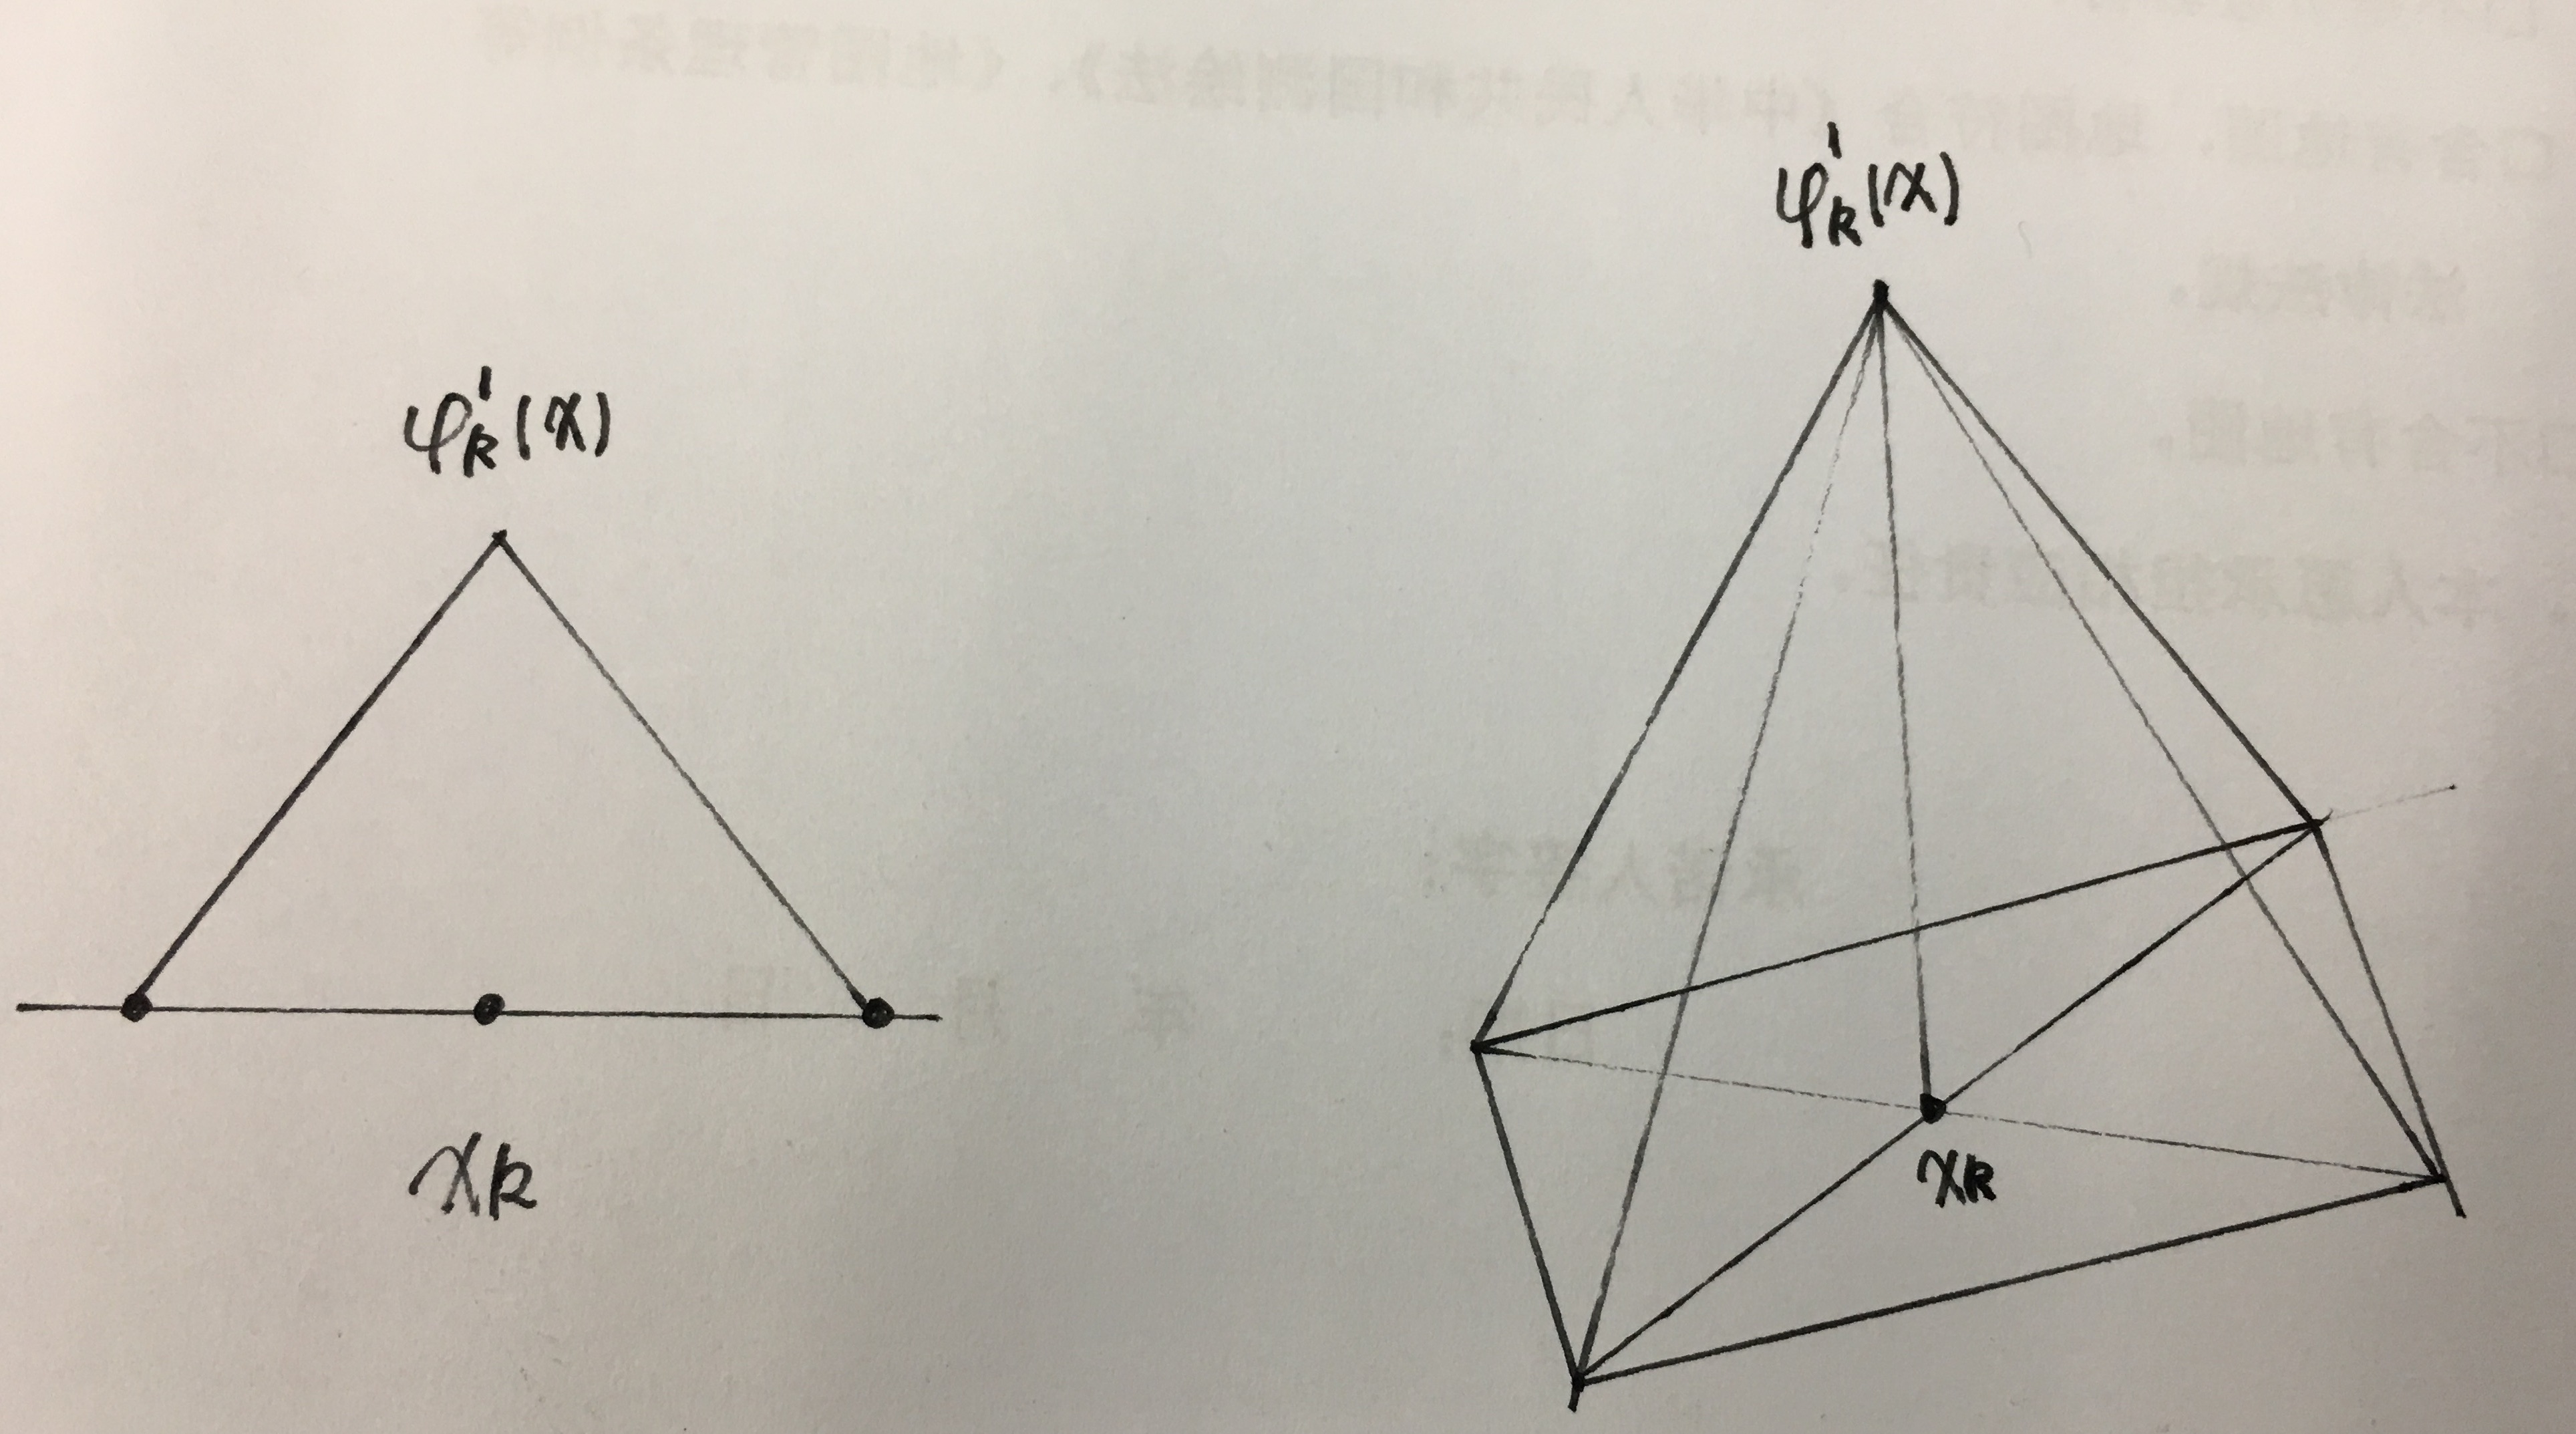
\includegraphics[width=4in]{./figures/20171214-trial-space-basis}
 \caption{检测空间$\mathcal{S}_{h}^{1}\left(\mathcal{T}_{N} \right)$的基$\psi_{k}^{1}(x)$}
\label{fig:finele-trial-basis}

%  \small{注:实线表示名义资金流动。虚线表示实际物质流动。}
\end{figure}


分段线性方程$\nu_{h}(x) \in \mathcal{S}_{h}^{1}\left(\mathcal{T}_{N} \right)$可以表示为
\begin{equation*}
  \nu_{h}(x) = \sum_{k=1}^{M} \nu_{k} \psi_{k}^{1}(x).
\end{equation*}

进而检测空间中的范数见下引理
\begin{lemma}[光谱等价范数不等式]
  \label{lemma:finele-trial-norm-spectral}
  $\nu_{h}(x) \in \mathcal{S}_{h}^{1}\left(\mathcal{T}_{N} \right)$在分解中的光谱等价范数不等式为
  \begin{equation}
    \label{eq:finele-trial-norm-spectral}
    \begin{split}
      \frac{1}{\left( d+1 \right)\left( d+2 \right)}
      \sum_{k=1}^{M}
      \left(\sum_{\ell \in I(k)} \Delta_{\ell} \right)
      \nu_{k}^{2}
      \le \left\|\nu_{h}\right\|_{L^{2}\left(\mathcal{T}_{N} \right)}
      \le \frac{1}{\left( d+1 \right)}
      \sum_{k=1}^{M}
      \left(\sum_{\ell \in I(k)} \Delta_{\ell} \right)
      \nu_{k}^{2}.
    \end{split}
  \end{equation}
\end{lemma}
\begin{proof}
  由Lemma \ref{lemma:finele-form-lin-norm-def}可得
  \begin{equation*}
    \begin{split}
      \left\| \nu_{h} \right\|_{L^{2} \left( \mathcal{T}_{N} \right)}^{2}
      & = \sum_{\ell}^{N} \left\| \nu_{h} \right\}
      \left\| \nu_{h} \right\|_{L^{2} \left( \mathcal{T}_{\ell} \right)}^{2} \\
      & \le \sum_{\ell=1}^{N}
      \frac{\Delta_{\ell}}{d+1} \,
      \sum_{k=1}^{d+1} \nu_{\ell_{k}}^{2} \\
      & = \frac{1}{d+1} \,
      \sum_{k=1}^{M} \left( \sum_{\ell \in I(k)}  \Delta_{\ell} \right)
      \nu_{k}^{2}
    \end{split}
  \end{equation*}
  为上限界。采用类似的方法可得下限界。证得\eqref{eq:finele-trial-norm-spectral}。
\end{proof}

\begin{lemma}[逆等价范数不等式]
  \label{finele-trial-norm-inverse}
  $\nu_{h}(x) \in \mathcal{S}_{h}^{1}\left(\mathcal{T}_{N} \right)$在分解中的逆等价范数不等式为
  \begin{equation}
    \label{eq:finele-trial-norm-inverse-local}
    \left\| \triangledown_{x} \nu_{h} \right\|_{L^{2} \left(\mathcal{T}_{N} \right)}^{2}
    \le c_{I} \sum_{\ell=1}^{N} h_{\ell}^{-2} \,
    \left\| \nu_{h} \right\|_{L^{2}(\tau_{\ell} )}^{2}.
  \end{equation}

  如果分解是全局拟一致的\index{quansi-uniform!globally \dotfill 全局拟一致},见\eqref{eq:finele-ref-quasi-uniform},那么我们有
  \begin{equation}
    \label{eq:finele-trial-norm-inverse-global}
    \left\| \triangledown_{x} \nu_{h} \right\|_{L^{2} \left(\mathcal{T}_{N} \right)}
    \le c \, h^{-1} \,
    \left\| \nu_{h} \right\|_{\left( \mathcal{T}_{N} \right)}.
  \end{equation}
\end{lemma}
\begin{proof}
可由Lemma  \ref{lemma:finele-form-norm-gradient}直接求得。
\end{proof}

为了求得检测空间$\mathcal{S}_{h}^{1}\left(\mathcal{T}_{N} \right)$的近似特性,首先要定义相应的插值算子和投影算子,然后计算误差测度项。
\subsubsection{检测空间的插值算子}
\label{sec:finele-trial-interpolation}
设$\nu \in C \left( \mathcal{T}_{N} \right)$是一个全局连续的方程。在含有分段线性方程的空间中定义插值如下
\begin{equation}
  \label{eq:finele-trial-interpolation}
  I_{h} \nu(x) \coloneqq \sum_{k=1}^{M} \nu(x_{k}) \varphi_{k}(x) \in  \mathcal{S}_{h}^{1}\left(\mathcal{T}_{N} \right).
\end{equation}

\begin{lemma}[分段线性插值的局部误差测度项]
  \label{lemma:finele-trial-interpolation-error}
  设给定的$\nu_{|_{\tau_{\ell}}} \in H^{2}\left( \tau_{\ell} \right)$。则我们有局部误差测度项
  \begin{equation}
    \label{eq:finele-trial-interpolation-error}
    \left\| \nu - I_{h} \nu \right\|_{L^{2}(\tau_{\ell})}
    \le c \, h_{\ell}^{2} \, \left| \nu \right|_{h^{2}(\tau_{\ell})}.
  \end{equation}
\end{lemma}
\begin{proof}
  \begin{enumerate}
  \item 根据识别方程等价范的测度不等式Theorem \ref{theorem:finele-ref-d123-norm-equiv}可得
  \begin{equation*}
  \left\| \nu - I_{h} \nu \right\|_{L^{2}(\tau_{\ell})}
  \le c \, \Delta_{\ell} \,
  \left\| \widetilde{\nu}_{\ell} - I_{\tau} \widetilde{\nu}_{\ell} \right\|_{L^{2}(\tau)},
  \end{equation*}
  其中$I_{\tau}:H^{2}(\tau) \mapsto L^{2}(\tau)$是相应参考元$\tau$的线性插值算子,满足
  \begin{equation*}
    \left\| I_{\tau} \widetilde{\nu}_{\ell} \right\|_{L^{2}(\tau)}
    \le \meas(\tau) \, \left\| \widetilde{\nu}_{\ell} \right\|_{L^{\infty}(\tau)},
  \end{equation*}
  $\meas(\tau)$表示$\tau$的测度(measure)。
  由索伯列夫嵌入定理(第\pageref{sec:imbedding-sobolev}页\ref{sec:imbedding-sobolev}节)可得
  \begin{equation*}
    \left\| \widetilde{\nu}_{\ell} \right\|_{L^{\infty}(\tau)}
    \le c \, \left\| \widetilde{\nu}_{\ell} \right\|_{L^{2}(\tau)},
  \end{equation*}
  可见$I_{\tau}:H^{2}(\tau) \mapsto L^{2}(\tau)$有界。

  \item 对于任意且固定的方程$\omega \in L^{2}(\tau)$,可定义一个线性泛函如下
  \begin{equation*}
    f(u) \coloneqq \int_{\tau} \left[
    \left( I - I_{\tau} \right) u(\xi)
    \right] \omega(\xi) d \xi.
  \end{equation*}

  如果给定方程$u \in H^{2}(\tau)$,那么我们有
  \begin{equation*}
    \begin{split}
      \left| f(u) \right|
      & = \left|
      \int_{\tau} \left[
      \left( I - I_{\tau} \right) u(\xi)
      \right]
      \omega(\xi) \, d \xi
      \right| \\
      & \le \left\|
      \left( I - I_{\tau} \right) u
      \right\|_{L^{2}(\tau)} \,
      \left\| \omega \right\|_{L^{2}(\tau)} \\
      & \le c \, \left\| u \right\|_{H^{2}(\tau)} \, \left\| \omega \right\|_{L^{2}(\tau)},
    \end{split}
  \end{equation*}
  即线性泛函$f$有界。

  对于任一线性方程$q \in \mathcal{P}_{1}(\tau)$,我们有$I_{\tau} q = q$,因此
  \begin{equation*}
    f(q) = 0, \quad \forall \, q \in \mathcal{P}_{1}(\tau).
  \end{equation*}

  可见Bramble-Hilbert引理 Lemma \ref{lemma:bramble-hilbert-lemma}的全部前提条件均得到满足。根据该引理可得
  \begin{equation*}
    \left| f(u) \right| \le \widetilde{c} \, \left\| \omega \right\|_{L^{2}(\tau)} \, \left| u \right|_{H^{2}(\tau)}.
  \end{equation*}

  \item 定义$u(\xi)$和$\omega(\xi)$的值如下
  \begin{equation*}
    \begin{cases}
      u \coloneqq \widetilde{\nu}_{\ell}, \\
      \omega \coloneqq \left( I - I_{\ell} \right) \widetilde{\nu}_{\ell},
    \end{cases}
  \end{equation*}

  进而
  \begin{equation*}
    \begin{split}
      \left\| \omega \right\|_{L^{2}(\tau)}^{2}
      & = \int_{\tau} \left( \omega (\xi) \right)^{2} d \xi
      = \int_{\tau} \left[
      \left( I - I_{\tau} \right)
      \widetilde{\nu}_{\ell}(\xi)
      \right] \omega(\xi) \, d \xi
      = \int_{\tau} \left[
      \left( I - I_{\tau} \right) u(\xi)
      \right]
      \omega(\xi) \, d \xi
      = \left| f \left( \widetilde{\nu}_{\ell} \right) \right| \\
      & \le \widetilde{c} \,
      \left\| \omega \right\|_{L^{2}(\tau)}
      \left| \widetilde{\nu}_{\ell} \right|_{H^{2}(\tau)} = \widetilde{c} \,
%      \underbrace{
      \left\| \left( I - I_{\tau} \right) \widetilde{\nu}_{\ell} \right\|_{L^{2}(\tau)}
%      }_{\eqqcolon \mathcal{A}} \,
      \, \left| \widetilde{\nu}_{\ell} \right|_{H^{2}(\tau)},
    \end{split}
  \end{equation*}
  \begin{equation*}
    \hookrightarrow
    \left\| \left( I - I_{\tau} \right) \widetilde{\nu}_{\ell} \right\|_{L^{2}(\tau)} \le \widetilde{c} \, \left| \widetilde{\nu}_{\ell} \right|_{H^{2}(\tau)}.
  \end{equation*}
  \item 代入Theorem \ref{theorem:finele-ref-d123-norm-equiv}可得
  \begin{equation*}
    \begin{split}
      \left\| \nu - I_{h} \nu \right\|_{L^{2}(\tau)}
      & \le c \, \Delta_{\ell} \,
      \left\| \widetilde{\nu}_{\ell} \right\|_{H^{2}(\tau)} \\
      & \le \hat{c} \, h_{\ell}^{2} \, \left| \nu \right|_{H^{2}(\tau_{\ell})}.
    \end{split}
  \end{equation*}
\end{enumerate}
\end{proof}

由Lemma \ref{lemma:finele-trial-interpolation-error}可得分段线性插值的全局误差项
\begin{equation}
  \label{eq:finele-trial-interpolation-error-global-L}
  \left\|
  \nu - I_{h} \nu
  \right\|_{L^{2}(\mathcal{T}_{N})}^{2}
  \le c \, \sum_{\ell=1}^{\ell} h_{\ell}^{4} \, \left| \nu \right|_{H^{2}(\tau_{\ell})}^{2},
\end{equation}
以及
\begin{equation}
  \label{eq:finele-trial-interpolation-error-global-H}
  \left\|
  \nu - I_{h} \nu
  \right\|_{H^{1}(\mathcal{T}_{N})}^{2}
  \le c \, \sum_{\ell=1}^{\ell} h_{\ell}^{2} \, \left| \nu \right|_{H^{2}(\tau_{\ell})}^{2}.
\end{equation}

\subsubsection{检测空间的投影算子}
\label{sec:finele-trial-projection}
为了应用插值算子执行上述运算,需要假定待差值的方程$\nu \in C \left( \mathcal{T}_{N} \right)$是全局连续的,这个假设过于强硬,有时较难满足。一个替代方案是以下若假设:

\part{模型估计}


\part{待分类}
%!TEX root = ../DSGEnotes.tex
\chapter{最大似然估计}
\label{sec:mle-model}

\epigraph{The maximum-likelihood procedure in any problem is what you are most likely to do if you don’t know any statistics.}{\textit{Harrison H. Barrett \\ Foundations of Image Science}}

\section{线性模型}
\label{sec:linear-model}

设一组含有$n$个观察数据的随机变量$\left\{ y_{i} \right\}, \, i = 1,\ldots,n$。假定其中每个观察符合正态分布$y_{i} \sim \mathcal{N} \left( \mu_{i}, \sigma^{2} \right)$。由设定可见,对于$i,j \in [1,n], \, i \neq j$,均值也许不同,但方差相同。

正态分布(normal distribution)\index{normal distribution! \dotfill 正态分布}又称高斯分布(Gaussian distribution)\index{Gaussian distribution \dotfill 高斯分布},如$y_{i}$的概率密度方程(probability density function, PDF)\index{probability density function (PDF) \dotfill 概率密度方程} $f\left( y_{i} \right)$定义为
\begin{equation}
  \label{eq:mle-pdf-def}
  f \left( y_{i} \right) = \frac{1}{\sqrt{2 \pi \sigma^{2}}}
  \exp \left[
  - \frac{1}{2} \frac{
  \left( y_{i} - \mu_{i} \right)^{2}
  }{
  \sigma^{2}
  }
   \right],
\end{equation}
均值为$0$方差为$1$的高斯分布,见图\ref{fig:mle-pdf}所示。

\begin{lstlisting}[language=R]
# 正态分布的概率密度方程(均值=0,方差=1)
x <- seq(-4,4,length=100)
hx <- dnorm(x)
plot(hx ~ x, type="l", lty = 1, col="blue",
     xlab="y", ylab="Density",
     main = "Probability Density Function (normal distribution)")
\end{lstlisting}

\begin{figure}[htbp]
  \caption{正态分布的概率密度方程}
  \centering
  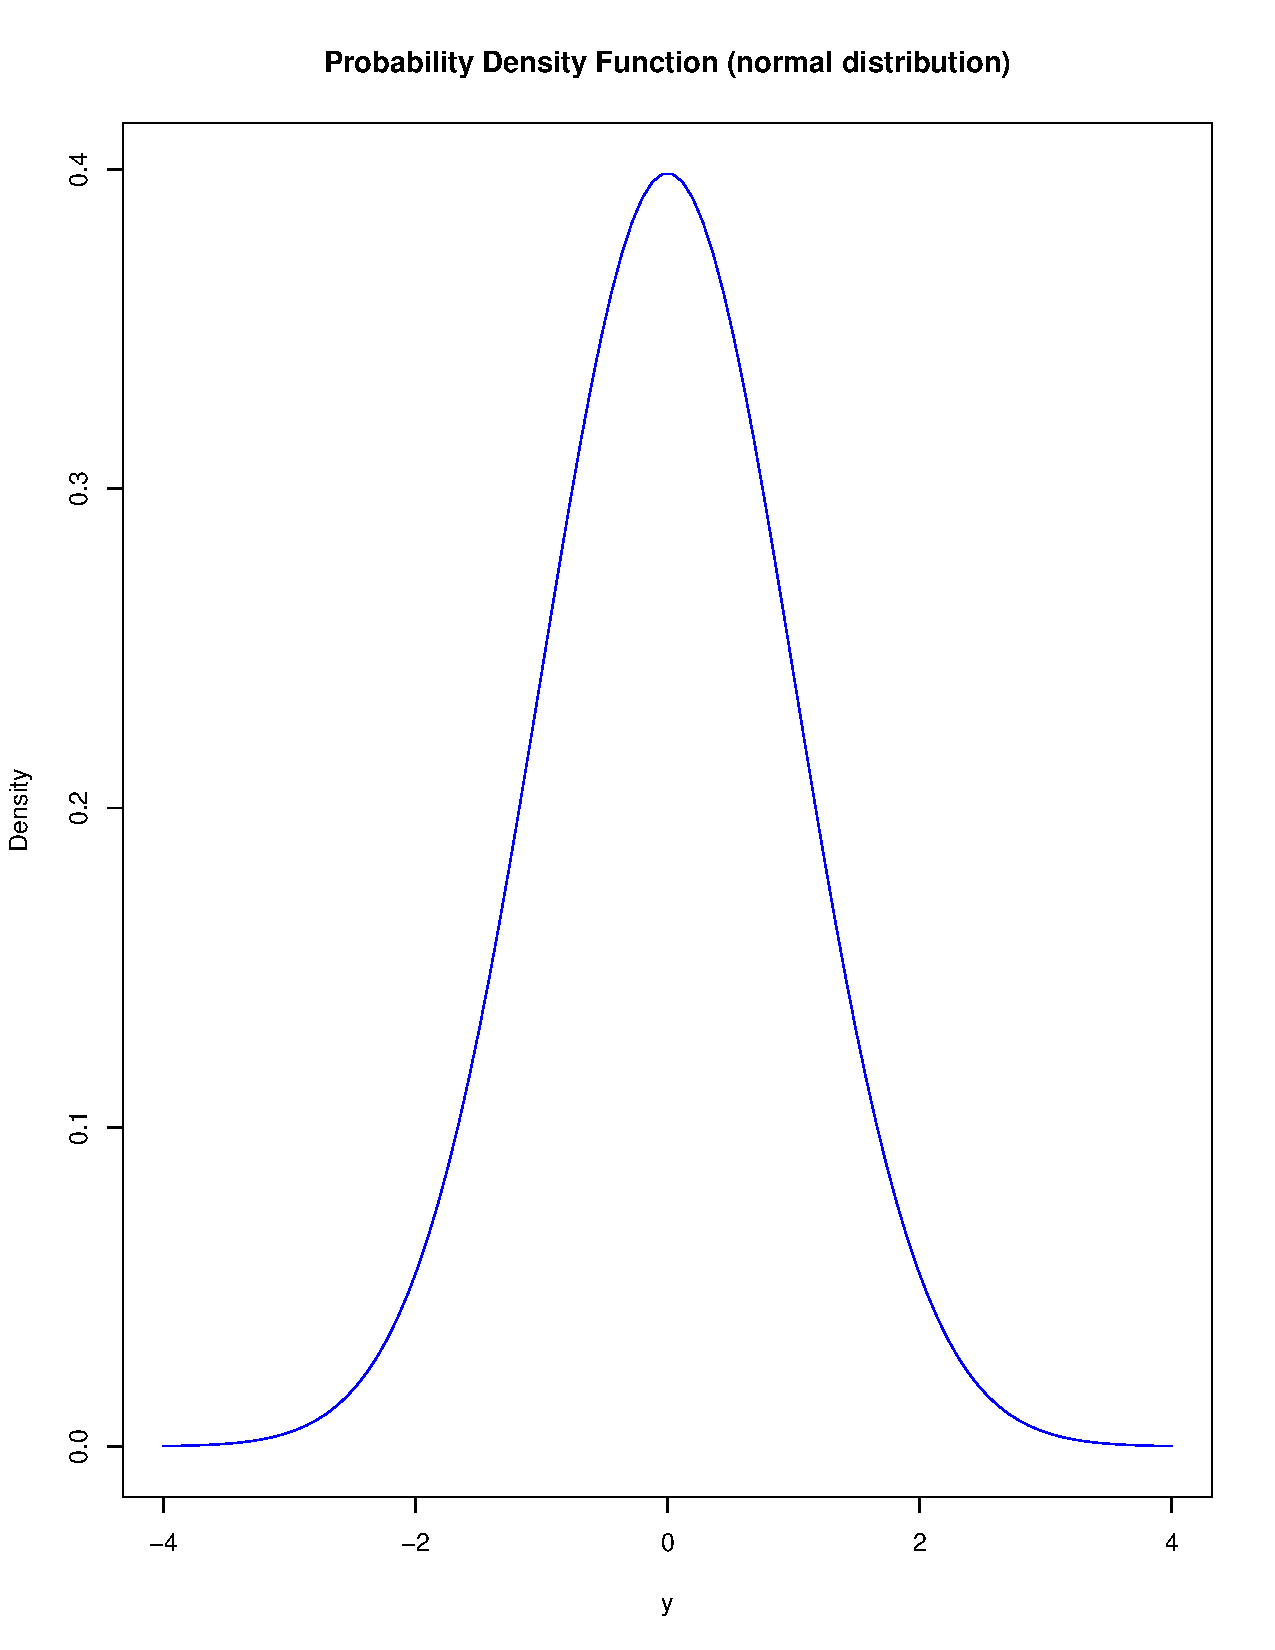
\includegraphics[width=8cm]{./Figures/20180421-pdf-function}
  \label{fig:mle-pdf}
%
%  \small{Source: PBOC.}
\end{figure}

现在引入额外的假定,对于全部$i, j \in [0,n], \, i \neq j$,设观测数据$y_{i}$和$y_{j}$相互独(mutually independent),即$\cov \left( y_{i}, y_{j} \right) = 0$。这使得我们能够计算观测数据集中全部数据的联合分布(joint distribution),即$\prod_{i=1}^{n} f \left( y_{i} \right)$,进而勾勒出似然方程,用于进一步的估计和检测。

把$\left\{y_{i}\right\}_{i=1}^{n}$表示为一个$(n \times 1)$的列向量$Y$,对应均值$E Y = \mu$,方差协方差矩阵$\var(Y) = \sigma^{2} I$,其中$I$是单位矩阵。列向量$\mu = \left\{ \mu_{i} \right\}_{i=1}^{n}$。
由于$n$个观测变量$y_{i}$彼此不相关且方差相同,$\var(Y)$满足以下特征:对角元素全是$\sigma^{2}$,非对角元素全是$0$。进而$Y$呈多元正态分布(multivariate normal distribution)\index{normal distribution!multivariate \dotfill 多元正态分布}
\begin{equation}
  \label{eq:multivariate-normal-distribution}
  Y \sim \mathcal{N}_{n} \left( \mu, \sigma^{2} I \right).
\end{equation}

来看\eqref{eq:multivariate-normal-distribution}的模型。假定$Y = y_{1}, y_{2}, \ldots, y_{n}$与某组预测变量$X = x_{1}, x_{2}, \ldots, x_{n}$有关,进一步说,第$i$个观测变量$y_{i}$的期望值$\mu_{i}$,与$x_{i1}, x_{i2}, \ldots, x_{ip}$有关,呈线性关系,满足
\begin{equation}
  \label{eq:mle-linear-relationship-yx-np}
  \mu_{i} = \beta_{1} x_{i1} + \beta_{2} x_{i2} + \ldots + \beta_{p} x_{ip} \Longleftrightarrow \mu_{i} = x_{i}^{\top} \beta,
\end{equation}
其中$x_{i}^{\top}$是由$p$个预测变量$x_{i1}, x_{i2}, \ldots ,x_{ip}$组成的行向量。待求解的未知系数$\beta = \beta_{1}, \ldots, \beta_{p}$称回归系数。将全部$n$个\eqref{eq:mle-linear-relationship-yx-np}加总可得
\begin{equation}
  \label{eq:mle-linear-relationship-mu-x-beta}
  \underset{\left( n \times 1 \right)}{\mu} =
  \underset{\left( n \times p \right)}{X}
  \underset{\left( p \times 1 \right)}{\beta},
\end{equation}
我们常将解释变量的矩阵$X$称为模型矩阵(model matrix)\index{model matrix \dotfill 模型矩阵}或设计矩阵(design matrix)\index{design matrix \dotfill 设计矩阵}。对应地,$X \beta$称线性预测子(linear predictor)。

最简单的线性模型可以假定每个观测数据的期望值都相同$\mu_{i} = \mu \, \forall \, i$,称零模型(null model)\index{null model \dotfill 零模型}。另一个极端是$\mu_{i} \neq \mu_{j} \, \forall \, i \neq j$,称饱和模型(saturated model)\index{saturated model \dotfill 饱和模型},此时观测数据量$n$越大,待估计的线性系数$\beta$数量就越多($p \times n$)。

零模型和饱和模型是两个极端。现实应用中常取折中,致力于分析导致线性预测子$X \beta$产生结构差异的系统性原因,进而分析观测数据$y$和均值$\mu$之间的非结构性差异(或称随机差异),用误差项来表示。

\section{参数估计}
\label{sec:mle-parameter-estimation}
来看模型$\mu_{i} = x_{i}^{\top} \beta$。问题:如何估计参数$\beta, \sigma^{2}$?

\subsection{回归系数的估计}
\label{sec:mle-estimation-beta}
我们的求解思路是,建立似然方程(likelihood function, LHF)\index{likelihood function (LHF)\dotfill 似然方程},选取使(对数)似然方程最大化的参数值。如果观测数据之间互相独立,那么LHF是一组正态PDF \eqref{eq:mle-pdf-def}的乘积
\begin{equation}
  \label{eq:mle-lhf-pdf-product}
  \log L \left( \beta, \sigma^{2} \right) = - \frac{n}{2} \log \left( 2 \pi \sigma^{2} \right) - \frac{1}{2} \sum_{i=1}^{n}
  \frac{
  \left( y_{i} - \mu_{i} \right)
  }{
  \sigma^{2}
  },
\end{equation}
$\mu_{i}$如\eqref{eq:mle-linear-relationship-yx-np}所定义。RHS中可定义残差平方和(residual sum of squares, RSS)\index{residual sum of squares (RSS) \dotfill 残差平方和}
\begin{equation}
  \label{eq:mle-rss-def}
  RSS (\beta) = \sum_{i=1}^{n} \left( y_{i} - \mu_{i} \right)^{2}
  = \left( y - X \beta \right)^{\top} \left( y - X \beta \right).
\end{equation}

不难看出,在给定$\sigma^{2}$值不变的情况下,最佳系数$\hat{\beta}$的选取符合
\begin{equation}
  \label{eq:mle-lhf-argmax-beta}
  \hat{\beta} =\underset{\beta}{\argmax} \log L \left( \beta, \sigma^{2} \right)
  = \underset{\beta}{\argmin} \frac{\rss(\beta)}{\sigma^{2}},
\end{equation}
也即,我们的目标是选取合适的$\beta = \hat{\beta}$,使对应的模拟值$\mu_{i}$尽可能接近实际观测值$y_{i}$。

求解$\argmin \rss (\beta)$等价于求解$\rss \left( \hat{\beta} \right) =0$,即
\begin{equation*}
  y - X \hat{\beta} = 0 \quad \Rightarrow y = X \hat{\beta} \quad \Rightarrow X^{\top} y = X^{\top} X \hat{\beta}
\end{equation*}
如果模型矩阵$X$列满秩,那么$X^{\top} X$也是满秩的,因而$X^{\top} X$可逆。由此可得线性系数$\hat{\beta}$的OLS估计式(同时也是MLE估计式)
\begin{equation}
  \label{eq:mle-argmin-beta-hat-estimation}
  \hat{\beta} = \left( X^{\top} X \right) X^{\top} y.
\end{equation}
我们将这个方程称为正规方程(normal equation)\index{normal equation \dotfill 正规方程}。

反之,如果$X$不是列满秩的,可以计算$\left( X^{\top} X \right)^{\dagger}$,称为伪逆矩阵(第\ref{sec:simple-pseudo}节)。但比起这种相对复杂的计算来,还是直接删除$X$中的冗余列更加方便。当前大多数主流统计软件都足够只能,可以自动识别并删除冗余列。

求解正规方程\eqref{eq:mle-argmin-beta-hat-estimation}需要借助数值方法。数值方法有多种,常见的如
\begin{itemize}
  \item 从$\left( X^{\top} X \right)$入手,方法如高斯消元法(第\ref{sec:numlin-gaussian-elimination}节)、Cholesky分解(第\ref{sec:numlin-factorization-cholesky}节)等。
  \item 对模型矩阵$X$做因子分解,如
  \begin{itemize}
    \item Householder reflections
    \item Givens rotations
    \item Gram-Schmidt正交(第\ref{sec:orthogonality-polynomials}节),等
  \end{itemize}
\end{itemize}
结合大多数主流数值计算软件,可以执行上述数值运算。

基于\eqref{eq:mle-lhf-argmax-beta},利用最小化RSS方法测得的系数$\hat{\beta}$,是一个不依赖于$\sigma^{2}$的值——方差值是事先给定的。因此我们称$\hat{\beta}$为最大似然法的全局最大解(global maximum)。

对于零模型的情况:$X$是一组$1$构成的向量;$\left( X^{\top} X \right) = n$和$X^{\top} y = \sum_{i=1}^{n} y_{i}$是两个标量;$\hat{\beta} = \bar{y}$是样本的均值。这就是说,计算出的样本均值,可堪称是在线性模型中做最大似然估计的一个最简单的例子。

关于MLE $\hat{\beta}$,有以下几个有趣的性质。

\begin{enumerate}
\item BLUE
\begin{enumerate}
  \item 如果模型设定正确,即从(弱的)意义上说,给定$x_{i}$的情况下,观测$y_{i}$的期望值$\mu_{i}$就等于$x_{i}^{\top} \beta$,此时的OLS估计$\hat{\beta}$是个无偏估计(unbiased estimator),OLS 估计$\hat{\beta}$的期望值就等于真实参数值$\beta$
\begin{equation}
  \label{eq:mle-hat-beta-unbiased}
  E \hat{\beta} = \beta.
\end{equation}
  \item 如果观测数据之间彼此不相关$\cov \left(y_{i}, y_{j} \right) = 0, \, \forall \, i \neq j$,并且同方差$\sigma_{i}^{2} = \sigma_{j}^{2}= \sigma^{2}$。那么,一方面根据\eqref{eq:mle-rss-def}-\eqref{eq:mle-lhf-argmax-beta},$\hat{\beta}$是一个关于$y$的线性方程,另一方面根据假定,观测数据集合$Y$的方差协方差矩阵$\var(Y) = \sigma^{2} I$,那么OLS估计$\hat{\beta}$的方差协方差矩阵为
  \begin{equation}
    \label{eq:mle-hat-beta-varcov}
    \var \left( \hat{\beta} \right) = \left( X^{\top} X \right)^{-1} \sigma^{2},
  \end{equation}
  因此,基于观测数据,构建线性方程模型所做的全部无偏OLS估计$\left\{\beta\right\}$中,MLE估计$\hat{\beta}$是最佳线性无偏估计(best linear unbiased estimator, BLUE)\index{best linear unbiased estimator (BLUE) \dotfill 最佳线性无偏估计}。对于某一给定的观测样本,由于再没有其他无偏估计的方差会低于$\var \left( \hat{\beta} \right)$,我们称OLS估计$\hat{\beta}$是有效估计(efficient estomator)\index{efficient estimator \dotfill 有效估计}。
\end{enumerate}

\item OLS估计$\hat{\beta}$在大样本观测集合中的抽样分布,接近于多元正态分布,其均值和方差如\eqref{eq:multivariate-normal-distribution}所定义,满足
\begin{equation*}
  \hat{\beta} \sim \mathcal{N}_{p} \left( \beta, \left(X^{\top}, X \right)^{-1} \sigma^{2} \right).
\end{equation*}

\item 将前两个性质代入零模型,可见样本均值$\bar{y}$是对$\mu$的无偏估计;$\bar{y}$的方差为$\frac{\sigma^{2}}{n}$,在大样本下近似正态分布。

\item 前三条性质的生成,依赖于对观测数据的均值、方差协方差的最高到二阶矩条件的假设,包括
\begin{equation*}
  E Y = X \beta, \quad \var \left( Y \right) = \sigma^{2} I.
\end{equation*}

\item 基于观测数据的联合正态分布假定,所测得的OLS估计$\hat{\beta}$也是MLE。如果$Y \sim \mathcal{N}_{p} \left( X \beta, \sigma^{2} I \right)$,那么$\hat{\beta}$的样本分布恰好也是多元正态分布,对应的、方差也是
\begin{equation*}
  \hat{\beta} \sim \mathcal{N}_{p} \left( \beta, \left(X^{\top}, X \right)^{-1} \sigma^{2} \right).
\end{equation*}.
\end{enumerate}

需要指出的是,上属性质虽然重要,但不应被过分夸大:只有在小样本数据的统计推断中,才需要假定观测数据是正态分布的。而真正重要的假设其实是观测数据之间彼此不相关,同方差:这些对于大样本数据下的统计推断至关重要。

\subsection{方差的估计}
\label{sec:mle-estimation-variance}
将求得的OLS估计$\hat{\beta}$ \eqref{eq:mle-argmin-beta-hat-estimation}代回log LHF \eqref{eq:mle-lhf-pdf-product},可得一个关于方差$\sigma^{2}$的最大(对数)似然方程,又称描述似然方程(profile likelihood function)\index{profile likelihood function \dotfill 描述似然方程}
\begin{equation}
  \label{eq:mle-estimation-variance-plhe}
  \log L \left( \sigma^{2} \right)
  = - \frac{n}{2} \log \left( 2 \pi \sigma^{2} \right)
  - \frac{1}{2} \frac{
  \rss \left( \hat{\beta} \right)
  }{\sigma^{2}}.
\end{equation}

类似地,$\hat{\sigma}^{2} = \underset{\sigma^{2}}{\argmax} \, \log L \left( \sigma^{2} \right)$,等价于求解$\frac{\partial \log L \left( \sigma^{2} \right)}{\partial \sigma^{2}} = 0 $,求得的值为方差的MLE
\begin{equation*}
  \hat{\sigma}^{2} = \frac{\rss \left( \hat{\beta} \right)}{n},
\end{equation*}
需要指出的是,$\hat{\sigma}^{2}$是有偏估计;我们可以将分母用$n-p$代替$n$来变为无偏估计(类似于在估计方差时用$n-1$代替$n$)。

在零模型中,方差$\sigma^{2}$的估计是样本方差:这是由于$\hat{\beta} = \bar{y}, \, \rss = \sum_{i=1}^{n} \left( y_{i} - \bar{y} \right)$。在正态分布的假定条件下,比值$\left( \frac{\rss }{\sigma^{2}}\right)$呈$\chi^{2}$分布(DoF n-p),并且与线性系数估计值$\hat{\beta}$无关。

小提示:使用$\chi^{2}$分布作为LHF来估计$\sigma^{2}$,比起使用高斯分步来同时估计$\beta, \sigma^{2}$来,会得到无偏估计。

\section{假设检验}
\label{sec:mle-hypothesis-testing}
如何对回归系数向量估计$\hat{\beta}$作假设检验?具体来说,这个问题可以分为两种情况
\begin{itemize}
  \item 对向量$\beta$中的某个系数$\beta_{i}$作显著程度检验,
  \item 对几个、甚至全部系数作显著程度检验,
\end{itemize}
本节介绍一些常见的检测方法,尤其是
\begin{itemize}
  \item 基于MLE的抽样分布的Wald检验,
  \item 似然率检验。
\end{itemize}

\subsection{Wald检验}
\label{sec:mle-wald-test}
假设我们只检测系数向量$\beta$中某一系数$\beta_{j}$的显著性,如
\begin{equation*}
  H_{0}: \beta_{j} = 0,
\end{equation*}
如果零假设成立,那么其MLE $\hat{\beta}_{j}$的分布情况因此可写为$\sim \mathcal{N} \left( 0, \var \left( \hat{\beta}_{j} \right)  \right)$,
其中方差 $\var \left( \hat{\beta}_{j} \right) $是方差协方差矩阵
$\var \left( \hat{\beta} \right)$
\eqref{eq:mle-hat-beta-varcov}中第$j$个对角元素的值。那么可以考虑如下比值,定义为Wald 统计量$t$
\begin{equation}
  \label{eq:mle-wald-t-def}
  t_{j} = \frac{\hat{\beta}_{j}}{\sqrt{\var \left( \hat{\beta}_{j} \right)}},
\end{equation}
计算$t_{j}$的难度在于,\eqref{eq:mle-hat-beta-varcov}中全体方差$\sigma^{2}$常常未知。在实际应用中,常常将$\sigma^{2}$替换为无偏估计$\hat{\sigma}^{2}$
\begin{equation}
  \label{eq:mle-wald-hat-var}
  \hat{\sigma}^{2} = \frac{\rss \left(\hat{\beta}\right)}{n-p}.
\end{equation}

假设观测数据符合正态分布,$\hat{\sigma}^{2}$依照\eqref{eq:mle-wald-hat-var}计算,那么在零假设下$\hat{\sigma}^{2}$呈学生$t$分布(student's t distribution),DoF n-p。

具体来说,若观测数据的二阶弱假设条件(均值、方差、方差协方差)得到满足,那么$t$值 \eqref{eq:mle-wald-t-def}在大样本下近似为标准正态分布。这为大样本数据下的近似推断打下良好基础。

一些研究中,不考虑数据样本量的大小,直接将\eqref{eq:mle-wald-t-def}作为学生$t$统计,而且这值得进一步讨论。
\begin{enumerate}
  \item 若样本量大,假定条件``观测数据是否符合正态分布"的确不重要;
  \item 若样本量相对较小,那么正态分布的假定是否成立,对Wald检测是否有效会产生决定性影响。
  对于规模适中的观测样本,应当审慎使用$t$检测:Student's t值随着自由度趋近于无穷大而收敛至标准正态分布\footnote{如双边95$\%$的关键$t$值是2.09 (20 DoF),1.98 (100 DoF),而标准正态分布的关键$t$值是1.96 (100 DoF)。}。
\end{enumerate}

$t$值可用于描述一个系数估计的置信区间(confidence interval)\index{confidence interval \dotfill 置信区间},例如,某个真实系数值$\beta_{j}$以$100 \times \left( 1 - \alpha \right) \%$的置信率落在统计区间中
\begin{equation}
  \label{eq:mle-wald-confidence-interval}
  \hat{\beta}_{j} \pm t_{
  \frac{1-\alpha}{2}, n-p
  }
  \sqrt{\var \left( \hat{\beta}_{j} \right)}.
\end{equation}
其中$t_{
\frac{1-\alpha}{2}, n-p
}$表示$n-p$ DoF,$\alpha$样本大小的学生$t$双边分布的关键值。

Wald检验也可用于检测一组系数的联合置信区间。将系数向量$\beta$分解为两块
\begin{equation*}
  \underset{\left\{ 1 \times p \right\}}{\beta^{\top}} =
  \left(
  \underset{\left\{ 1 \times p_{1} \right\}}{\beta_{1}^{\top}},
  \underset{\left\{ 1 \times p_{2} \right\}}{\beta_{2}^{\top}}
  \right),
\end{equation*}

建立零假设
\begin{equation*}
  H_{0}:\beta_{2} = 0.
\end{equation*}

在求得MLE $\hat{\beta}$后,将Wald检验统计量表示为二次形式
\begin{equation}
  \label{eq:mle-wald-joint-statistic}
  W =
  \hat{\beta}_{2}^{\top}
  \left( \var \left( \hat{\beta}_{2} \right) \right)^{-1}
  \hat{\beta}_{2},
\end{equation}
如前所述,我们用$\frac{ \var \left( \hat{\beta} \right)}{n-p}$近似替代全$\sigma^{2}$,用于测算方差协方差矩阵$\var \left( \hat{\beta}_{2} \right)$。若$p_{2}=1$即$\beta_{2}$只有一个系数,那么\eqref{eq:mle-wald-joint-statistic}回复到
\eqref{eq:mle-wald-hat-var}的形式。

根据渐进理论(asymptotic theory),在零假设$H_{0}$下,大样本MLE $\hat{\beta}_{2}$符合多元正态分布,均值向量为$0$,方差协方差矩阵为$\var \left( \hat{\beta}_{2} \right)$。由此可得,二次形Wald统计$W$ \eqref{eq:mle-wald-joint-statistic}在大样本下也是一个$\chi^{2}$分布,对应$p_{2}$ DoF。无论$\sigma^{2}$是实现给定的值,还是利用$\rss$作近似估计,上述结论都成立。

如果我们持有更强形式的假定,即观测数据呈正态分布,那么检验的结果也是更强形式的。此时若$\sigma^{2}$值事先给定,$W$就恰好是$\chi^{2}$分布($p_{2}$ DoF)。若用$\frac{\rss \left( \hat{\beta} \right)}{n-p}$来近似估计$\sigma^{2}$ (对应$p_{2}$ DoF),则$\frac{W}{p_{2}}$呈一个对应于$p_{2}$和DoF $n-p$ 的$F$分布。

值得注意的是,给定$p$值不变,随着$n \rightarrow \infty$,$ \left( n-p \right) \rightarrow \infty$,$F_{p_{2}, n-p} \times p_{2} \rightarrow \chi^{2} \, \left( p_{2} \, DoF \right)$。这意味着在大样本情况下,将$W$统计量视作$\chi^{2}$分布,或是将$W/p_{2}$视作$F$分布,二者并无本质区别。

\subsection{似然率检验}
\label{sec:mle-lhr-test}
还来看多系数联合显著水平检验的例子,对应零假设
\begin{equation*}
  H_{0}:\beta_{2} =0.
\end{equation*}

我们可以将模型矩阵$X$相应地分解为
\begin{equation*}
  \underset{\left\{p \times 1 \right\}}{X} = \left(
  \underset{\left\{p_{1} \times 1 \right\}}{X_{1}},
  \underset{\left\{p_{2} \times 1 \right\}}{X_{2}}
  \right),
\end{equation*}
如果零假设成立,这意味着后面的$p_{2}$个解释变量$X_{2}$对观测数据$Y$无影响。

可以建立似然率检验(likelihood ratio test, LHR)指标,
对零假设做检验,分两步走
\begin{enumerate}
  \item 分别构建两个嵌入模型并作拟合。
  \begin{enumerate}
    \item 小模型:只考虑前$p_{1}$个解释变量$X_{1}$。
    \item 大模型:用全部$p = p_{1} + p_{2}$ 个解释变量$X$。
  \end{enumerate}
  \item 比较两个模型的最大(对数)似然方程。
\end{enumerate}

先来看只考虑$X_{1}$的小模型。基于给定的方差$\sigma^{2}$,对应似然方程\eqref{eq:mle-lhf-pdf-product},可得最大似然方程
\begin{equation}
  \label{eq:mle-mlh-small-model}
  \max \log L \left( \beta_{1} \right) = c - \frac{1}{2} \frac{\rss \left( X_{1} \right)}{\sigma^{2}}, \quad c = - \frac{n}{2} \log \left( 2 \pi \sigma^{2} \right),
\end{equation}
其中常数$c$的值取决于$n$和$\sigma^{2}$。

对应地,考虑$X = \left(X_{1}, X_{2} \right)$的大模型,最大似然方程
\begin{equation}
  \label{eq:mle-mlh-big-model}
  \max \log L \left( \beta_{1}, \beta_{2} \right)
  = c - \frac{1}{2} \frac{\rss \left( X_{1} + X_{2} \right)}{\sigma^{2}}.
\end{equation}

将两个最大似然方程\eqref{eq:mle-mlh-small-model},\eqref{eq:mle-mlh-big-model}相减,定义为$\log \lambda$,作为似然率量(likelihood ratio criterion, LHRC)\index{likelihood ratio criterion (LHRC) \dotfill 似然率量}
\begin{equation}
  \label{eq:mle-mlh-lhrc}
  - 2 \log \lambda = \max \log L \left( \beta_{1} \right) - \max \log L \left( X_{1}, X_{2} \right) = \frac{
  \rss \left( X_{1} \right) - \rss \left( X_{1} + X_{2} \right)
  }{
  \sigma^{2}
  }.
\end{equation}

关于LHRC,有两点说明
\begin{enumerate}
  \item 通过两个最大似然方程的差值,该指标反映在引入额外的$p_{2}$个解释变量$X_{2}$后,$\rss$的变化情况。通常来说,如果$\Delta \rss >0$,那么$X_{2}$对观测数据可能是有显著影响的。
  \item 对$\Delta \rss$除以方差$\sigma^{2}$是作单位标准化处理,表示残差平方和的变化是以总方差的单位计。如果这个比值(最大似然率)超过了事先预期值,就表示$X_{2}$的确是显著的,零假设不成立。
\end{enumerate}

这就涉及到如何设定``事先预期”值,它与样本的分布有关。根据大样本定律可知,随着$n \rightarrow \infty$,样本分布逐渐收敛至$\chi^{2}$ ($p_{2}$ DoF)。对于$\chi^{2}$分布,已知期望值和方差分别为$\nu$和$2 \nu$,那么事先预期的设定可以使:每增加额外$1$个变量$p_{2} \rightarrow p_{2} + 1$,会导致$\Delta \rss$减少$\sigma^{2}$个单位,对应标准化后的单位$1$。具体说来,若$\rss$的下降幅度超过$95\%$百分位(percentile)的参考分布值,就表示为误差的缩减超出预期。

类似地,LHRC \eqref{eq:mle-mlh-lhrc}的计算难度在于$\sigma^{2}$可能未知。可以用用大模型$\rss \left( X_{1} + X_{2} \right)$的方差估计$\hat{\sigma}^{2}$作近似替代,计算方法为
\begin{equation*}
  \hat{\sigma}^{2} = \frac{
  \rss \left( X_{1} + X_{2} \right)
  }{n-p},
\end{equation*}
代回\eqref{eq:mle-mlh-lhrc},算得的大样本下LHRC分布依旧是$\chi^{2}$分布($p_{2}$ DoF)。

若观测样本符合正态分布这一更强假定,结果也相应更强。如果$\sigma^{2}$是已知的,那么LHRC $- 2 \log \lambda$就恰好是$\chi^{2}$分布($p_{2}$ DoF)。如果$\sigma^{2}$未知,是用估计出的$\hat{\sigma}^{2}$作近似替代,那么对应的LHRC除以$p_{2}$,即$\frac{- 2 \log \lambda}{n-p}$就恰好是一个$F_{p_{2}, n-p}$分布,满足
\begin{equation}
  \label{eq:mle-mlh-lhrc-f}
  F = \frac{
  \frac{1}{p_{2}}
  \left[
  \rss \left( X_{1} \right) - \rss \left( X_{1} + X_{2} \right)
  \right]
  }{
  \frac{1}{n-p} \rss \left( X_{1} + X_{2} \right)
  },
\end{equation}
分子表示在每一单位自由度减少,导致$\rss$的减少幅度;分母是平均$\rss$,反映模型总体的噪声情况。通常来说,如果测得的$F$统计值高于$F$分布在$95\%$下对应$p_{2}, \, n-p$的关键值,那么我们可以拒绝零假设$H_{0}$,$X_{2}$的确对观测数据产生影响。

\subsection{Anova表}
\label{sec:mle-anova}
在实际应用中,到底应该用基于大样本分布下最大似然估计的Wald检验,还是基于最大(对数)似然估计比较的似然率检验呢?答案是,随着$n$值逐渐增大,两种检测方法渐进等价。若模型是线性的,则回答更为明确:两种检测完全等价。详细证明过程略,我们可以在一些具体应用中涉及相关讨论。

值得指出的是,两种检验的(渐进)等价基于模型的线性结构假定。对于非线性模型如logistic模型、泊松回归模型等,两种检测是有区别的。通常说来,对线性模型的检测而言,我们可以提出以下建议:
\begin{itemize}
  \item 对单个系数可用Wald检验 \eqref{eq:mle-wald-t-def},
  \item 多个系数的检验,或者进一步对多个嵌入模型的比较,可用LHRC的$F$检验 \eqref{eq:mle-mlh-lhrc-f}。
\end{itemize}

测算$F$统计所需的计算,常收录在anova表中(analysis of variance table, anova)\index{analysis of variance table (anova) \dotfill anova表}。表格将整体$\rss$分为三个部分,小模型$X_{1}$的$\rss$、加入$X_{2}$后大模型的$\rss$、剩余$\rss$。每个$\rss$项后还附有DoF,以及平均值$\frac{\rss}{DoF}$,如表\ref{table:mle-anova-table}所示。

\begin{table}[h]
\caption{anova表}
\begin{center}
\begin{threeparttable}
\begin{tabular}{c c c}
    \toprule
     & $\rss$ & DoF \\ \midrule
      $X_{1}$\tnote{a} & $\rss \left( \phi \right) - \rss \left( X_{1} \right)$ & $p_{1}-1$ \\
      $X_{2} | X_{1}$ \tnote{b} & $\rss \left( X_{1} \right) - \rss \left( X_{1} + X_{2} \right) $ & $p_{2}$  \\
      残差 & $\rss \left( \phi \right)$ & $n-p$  \\ \midrule
      全部\tnote{c}  & $\rss \left( X_{1} + X_{2} \right)$ & $n-1$  \\ \bottomrule
\end{tabular}
\tiny{
\begin{tablenotes}
\item[a] $\phi$表示零模型
\item[b] 有时我们需要更多的细节,那么可以将$p_{2}$个$X_{2}$分拆后一个一个加入到模型中,分别计算$\rss$和自由度
\item[c] 有时也称不相关$\rss$,即$= \sum_{i=1}^{n} y_{i}^{2}$
\end{tablenotes}
}
\end{threeparttable}
\end{center}
\label{table:mle-anova-table}
\end{table}

一系列信息如简单相关系数、偏相关系数、复相关系数(coefficients of simple, partial, multiple correlation)都可基于anova表中$\rss$和DoF的信息而计算获得。

几乎全部主流统计软件都支持数值计算anova。

\subsection{简单线性回归}
\label{sec:mle-slr}
先来看一个线性解释变量$x$对$y$的连续影响。若已知从观测数据来看,哪怕$x$是定值,对应的观测数据$y$也有所不同,那么可将$\left\{ y_{i} \right\}$ 理解为一组随机变量的实现
\begin{equation}
  \label{eq:mle-slr-distribution}
  y_{i} \sim \mathcal{N} \left( \mu_{i}, \sigma^{2} \right),
\end{equation}
其中均值$\mu_{i}=E y_{i}$取决于解释变量$x_{i}$,方差$\sigma^{2}$是个常数。最简单的思路可以假设一个线性方程,从而得到一个简单线性模型(simple linear regression model, SLRM)
\begin{equation}
  \label{eq:mle-slr-mu-x}
  \mu_{i} = \alpha + \beta x_{i},
\end{equation}
$\alpha$常称为常数项或结局想,反映$x_{i}=0$时,期望$\mu_{i}$的取值。$\beta$称为斜率,表示随着$x_{i}$的增加,期望$\mu_{i}$的变化幅度。

SLRM可以理解为一个一般线性模型(第\ref{sec:linear-model}节)的特例:模型矩阵$X$包括两列,一列是常数项$\alpha$,一列是解释变量$x_{i}$。可对参数做估计,计算标准差(第\ref{sec:mle-parameter-estimation}节),并执行假设检验(第\ref{sec:mle-hypothesis-testing}节)。

在SLRM中,$\alpha$和$\beta$的估计为
\begin{align}
\label{eq:mle-slrm-estimate-alpha}
  \hat{\alpha} & = \bar{y} - \hat{\beta} \bar{x}, \\
\label{eq:mle-slrm-estimate-beta}
  \hat{\beta} &= \frac{
  \sum_{i=1}^{n} \left( x_{i} - \bar{x} \right) \left( y_{i} - \bar{y} \right)
  }{
  \sum_{i=1}^{n} \left( x_{i} - \bar{x} \right)^{2}
  }.
\end{align}

拟合的直线\eqref{eq:mle-slrm-estimate-alpha}反映解释变量期望值和观测数据期望值之间的关系,对应斜率\eqref{eq:mle-slrm-estimate-beta}反映协方差$\cov \left( x_{i},y_{i} \right)$和方差$\var \left( x_{i} \right)$之间的比值。

[找个回归跑一下,做个说明。]

其中我们有决定系数(coefficient of determination)\index{coefficient of determination \dotfill 决定系数} $R^{2}$
\begin{equation*}
  R^{2} = 1 - \frac{
  \rss \left(x \right)
  }{
  \rss \left( \phi \right)
  },
\end{equation*}
对应地我们将$R$称为皮尔逊线性相关系数(Person's linear correlation coefficient)\index{Person's linear correlation coefficient \dotfill 皮尔逊线性相关系数}
\begin{equation}
  \label{eq:mle-slrm-pearson-coefficient}
  R = \frac{
  \sum_{i=1}^{n} \left( y_{i} - \bar{y} \right) \left( x_{i} - \bar{x} \right)
  }{\sqrt{
  \sum_{i=1}^{n} \left( y_{i} - \bar{y} \right)^{2} \,
  \sum_{i=1}^{n} \left( x_{i} - \bar{x} \right)^{2}
  }}
\end{equation}

现在,假设我们用两个解释变量向量$x_{1}, \, x_{2}$来解释观测向量$y$,其中第$i$个元素分别为$x_{i1}, \, x_{i2}, \, y_{i}, \, i=1,\ldots,n$。$y_{i}$设为$Y_{i} \sim \mathcal{N} \left( \mu_{i}, \sigma^{2} \right)$。那么我们有多元线性回归模型(multivariate regression model, MLRM)
\begin{equation}
  \label{eq:mle-mlrm-mu-x}
  \mu_{i} = \alpha + \beta_{1} x_{i1} + \beta_{2} x_{i2},
\end{equation}
构成一个三维空间。$\alpha$是常数,$\beta_{1}, \, \beta_{2}$分别是$x_{i1}, \, x_{i2}$的斜率。求解方法、参数估计和假设检验与SLRM相类似。

\section{回归诊断}
\label{sec:mle-regression}
通常来说,统计建模的工作分为三个阶段:模型构建、用模型拟合数据、模型诊断。在前两个阶段工作的基础上,模型诊断主要是指重新调整模型,使其能够更好地解释现实。本节介绍相关方法。

\subsection{拟合值与残差}
\label{sec:mle-regression-fitted-residual}
诊断模型用的指标是残差$r_{i}$,它是观测数据$y_{i}$和模拟数据$\hat{y}_{i} = X_{i}^{\top} \beta$之间的差
\begin{equation}
  \label{eq:mle-residual-def}
  r_{i} = y_{i} - \hat{y}_{i}, \, i=1,\ldots,n.
\end{equation}

如\eqref{eq:mle-linear-relationship-mu-x-beta}所示,将全部$i$个$\hat{y}_{i}$汇总在一起,有矩阵形式
\begin{equation*}
  \label{eq:mle-simulated-y-matrix}
  \hat{y} = X \hat{\beta}, \quad \hat{\beta}=\underset{\beta}{\argmin} \rss \left( \beta \right)
\end{equation*}
其中$X$是模型矩阵,$\rss \left( \beta \right)$的计算方式见\eqref{eq:mle-rss-def}。在此基础上我们有
\begin{equation}
  \label{eq:mle-simulated-y-h}
  \hat{y} = H y, \quad H = X \left( X^{\top} X \right)^{-1} X,
\end{equation}
其中$H: y \mapsto \hat{y}$又称帽子矩阵(hat matrix)\index{hat matrix \dotfill 帽子矩阵}。

根据这样的定义我们有,模拟值$\hat{y}$的均值$\mu$,方差协方差矩阵$\var \left( \hat{y} \right)$分别满足
\begin{equation*}
  \mu = E \hat{y}, \quad \var \left( \hat{y} \right) = H \, \sigma^{2}.
\end{equation*}

在此基础上,残差矩阵$r$满足
\begin{equation*}
  r = y - \hat{y},
\end{equation*}
其中$y, \, \hat{y}$分别表示观测值向量和模拟值向量。引入\eqref{eq:mle-simulated-y-h}替代$\hat{y}$,上式进一步变为
\begin{equation}
  \label{eq:mle-residual-hat}
  r = \left( I - H \right) \sigma^{2}.
\end{equation}

假设观测数据满足常见的二阶条件,那么我们有残差的均值和方差协方差矩阵
\begin{equation*}
  Y \sim \mathcal{N} \left( 0, \sigma^{2} \right) \Longrightarrow \begin{cases}
  E r =0 \\
  \var \left( r \right) = \left( I - H \right),
  \end{cases}
\end{equation*}
进而第$i$个残差$r_{i}$的方差
\begin{equation}
  \label{eq:mle-residual-var-i}
  \var \left( r_{i} \right) = \left( 1 - h_{ii} \right) \sigma^{2},
\end{equation}
其中$h_{ii}$是帽子矩阵$H$中第$i$个对角元素。

由\eqref{eq:mle-residual-var-i}可看出一个重要性质:尽管全部观测数据的方差相同$\sigma^{2}$,但具体每个观测残差的方差$\var \left( r_{i} \right)$却可能不相等,其原因在于模拟值$\hat{y}_{i}$的精度取决于协变量$x_{i}$的值,而后者并不相同。为了解决这个问题,随后提出了标准化残差的概念,见第\ref{sec:mle-std-residual}节。

来看$h_{ii}$的取值区间。假定模型的截距项不为$0$,那么我们有$h_{ii} \in \left[ \frac{1}{n}, \frac{1}{r} \right]$,其中$n \ni i$表示全部观测数据的数量,$r$表示第$i$个观测值的复制的数量,或者说,全部协变量值等于$x_{i}$的观测样本$i$的数量。在SLRM中,有
\begin{equation}
  \label{eq:mle-slre-hat-matrix-h-ii}
  h_{ii} = \frac{1}{n} + \frac{
  \left( x_{i} - \bar{x} \right)^{2}
  }{
  \sum_{i=1}^{n} \left( x_{i} - \bar{x} \right)^{2}
  },
\end{equation}
可见当$x_{i}$恰好等于其均值$\bar{x}$时,$h_{ii}$有最小值$\frac{1}{n}$。

值得指出的是,观测值$y_{i}$越是接近(远离)其均值$\bar{y}$,对应的模拟值$\bar{y_{i}}$的方差$\var \left( \bar{y}_{i} \right)$就越小(大)。但通过\eqref{eq:mle-residual-var-i}-\eqref{eq:mle-slre-hat-matrix-h-ii}可见,$x_{i}$越是接近(远离)$\bar{x}$,$h_{ii}$越小(大),残差的方差$\var \left( r_{i} \right)$就越大(小)。

\subsection{标准化残差}
\label{sec:mle-std-residual}
根据残差$r$的定义\eqref{eq:mle-residual-var-i}可见,在比较不同观测数据的残差$r_{i}, \, r_{j}, \, i,j=1,\ldots,n$时,需要注意可能存在$\var \left( r_{i} \right) \neq \var \left( r_{j} \right)$的情况,导致不同观测数据之间难于直接比较。因此可以调整如下,将$r_{i}$扩展为标准化残差$s_{i}$ (standardized residual)\index{standardized residual \dotfill 标准化残差}
\begin{equation}
  \label{eq:mle-std-residual-def}
  s_{i} = \frac{
  r_{i}
  }{\sqrt{
  1 - h_{ii}
  }\hat{\sigma}},
\end{equation}
其中$\hat{\sigma}$是基于$\rss$的标准差估计。

标准化残差$s_{i}$可用于检验观测样本中是否存在不规则观测值(anomalous observation)或称离群值(outlier)\index{outlier \dotfill 离群值}。通常来说,若某个观测值$y_{i}$的标准化残差绝对值$\left| s_{i} \right| > 2$,就需要对它额外关注:它可能是离群值(但并非绝对,详见第\ref{sec:mle-outlier}节讨论)。

\subsection{Jack-knifed残差}
\label{sec:mle-jackknifed-residual}
标准化残差$s_{i}$ 的不足在于,计算式\eqref{eq:mle-std-residual-def}中还依赖于标准差估计$\hat{\sigma}$:它可能受到离群值的影响,而离群值很可能不易检测出来。可进一步调整如下:将$r_{i}$用一个误差方差估计$\hat{\sigma}_{(i)}$替代$\hat{\sigma}$作标准化处理,称之为Jack-knifed残差(Jack-Knifed residual)\index{Jack-knifed residual \dotfill Jack-knifed残差}或学生化残差(studentized residual)\index{studentized residual \dotfill 学生化残差},用$t_{i}$表示
\begin{equation}
  \label{sec:mle-studentized-residual}
  t_{i} = \frac{r_{i}}{
  \sqrt{1 - h_{ii}} \hat{\sigma}_{(i)}
  },
\end{equation}
$\hat{\sigma}_{(i)}$的计算方法:值通过``遗漏"第$i$项观察元素,对剩下部分做模型拟合,基于$n-p-1$ DoF下$\rss$测得的标准差。需要注意的是,拟合值$\hat{y}$和帽子矩阵$H$的计算仍然基于含有第$i$观测样本。

\begin{definition}[标准化预测残差]
  \label{definition:standardized-predictive-residual}
如果用不含有$i$的观测数据,不只计算Jack-knifed残差 \eqref{sec:mle-studentized-residual},还计算标准残差,那么标准残差会发生什么变化?用$\hat{\beta}_{\left( i \right)}$表示回归系数的估计,建立估计模型
\begin{equation*}
  \hat{y}_{\left( i \right)} = x_{i}^{\top} \hat{\beta}_{\left( i \right)},
\end{equation*}
相应地我们将
\begin{equation*}
  y_{i}- \hat{y}_{ \left( i \right\}}
\end{equation*}
称预测残差(predictive residual)。预测残差的方差为
\begin{equation*}
  \var \left( y_{i}- \hat{y}_{ \left( i \right)} \right)
  = \left(
  1 + x_{i}^{\top}
  \left( X_{\left( i \right)}^{\top} \, X_{\left( i \right)}\right)^{-1}
  x_{i}
  \right) \sigma_{\left( i \right)}^{2},
\end{equation*}
由于第$i$项被剔除在回归分析之外,因此$y_{i}$和$\hat{y}_{\left( i \right)}$不相关。$X_{\left( i \right)}$是模型矩阵$X$去除掉第$i$行后剩余的部分。$\hat{\sigma}_{\left( i \right)}^{2}$是去掉第$i$项观测元素后,对余下部分构建模型,计算$\rss$,进而算得。用$\hat{\sigma}_{\left( i \right)}^{2}$近似未知的$\sigma^{2}$,可得标准化预测残差(standardized predictive residual)\index{standardized predictive residual \dotfill 标准化预测残差}
\begin{equation}
  \label{eq:standardized-predictive-residual}
  t_{i} = \frac{
  y_{i}- \hat{y}_{ \left( i \right) }
  }{
  \sqrt{\var \left(  y_{i}- \hat{y}_{ \left( i \right) } \right)}
  }.
\end{equation}
不难看出,标准化预测残差\eqref{eq:standardized-predictive-residual}和Jack-knifed残差\eqref{sec:mle-studentized-residual}等价,可以互换。
\end{definition}

Jack-knifed残差$t_{i}$ 的计算式\eqref{sec:mle-studentized-residual}较为复杂。在求得标准化残差$s_{i}$   \eqref{eq:mle-std-residual-def}的基础上,可将$t_{i}$计算简化为\citep{Cook:1982wb}
\begin{equation}
  \label{eq:standardized-predictive-residual-cook-weisberg}
  t_{i} = s_{i} \left(
  \frac{n-p-1}{n-p-s_{i}^{2}}
  \right)^{\frac{1}{2}},
\end{equation}
不难看出,$t_{i}$是一个关于$s_{i}$的单调方程,那么序列$\left\{ t_{i} \right\}_{i=1}^{n}$的排序,就等价于$\left\{ s_{i} \right\}_{i=1}^{n}$的排序。

\subsection{离群值的检测}
\label{sec:mle-outlier}
$s_{i}$或$t_{i}$的值大于2,暗示着$y_{i} \in Y, \, i = 1, \ldots, n$可能是离群值。仅仅``可能”不够精确,我们可以利用$t_{i}$作进一步诊断。对于原有的模型$\mu_{i} = X_{i}^{\top} \beta$作扩展,加入一个哑变量(dummy variable) $z_{i}$,从而允许第$i$个观测数据出现位移
\begin{equation*}
  \mu_{i} = X_{i}^{\top} \beta + \gamma z_{i}, \quad z_{i} = \begin{cases}
  1 & \text{是第i个观测} \\
  0 & \text{其他},
  \end{cases}
\end{equation*}
系数$\gamma$用于表示观测$y_{i}$可以在多大程度上偏离(由协变量$X_{i}$和回归系数$\beta$共同描述的)期望值$\mu_{i}$。

建立一个零假设用于检测$y_{i}$是不是离群值,即$y_{i}$是否与其他$n-1$个观测$\left\{ y_{1}, \ldots, y_{i-1}, y_{i+1}, \ldots, y_{n} \right\}$有相同的行为模式:
\begin{equation*}
  H_{0} : \gamma =0.
\end{equation*}

对系数$\gamma$作近似估计$\hat{\gamma}$。对$H_{0}$作Wald检验,算得的$t$就是Jack-knifed残差$t_{i}$值,自由度$\left( n-p-1 \right) $
\begin{equation}
  \label{eq:mle-outlier-jackknifed}
  t_{i} = \frac{
  \hat{\gamma}
  }{
  \sqrt{\var \left( \hat{\gamma} \right)}
  }.
\end{equation}

这一设定允许$\mu_{i}$拥有不同于其他$n-1$个观测均值的特征,用估计系数$\hat{\gamma}$表示。我们事实上是在用除$i$之外的$n-1$个观测来估计$\hat{\beta}$,用全部$n$个观测来估计$\hat{\gamma}$,从这个意义上来讲$\gamma$描述的信息与预测残差 (Definition \ref{definition:standardized-predictive-residual})相近。

在利用Jack-knifed残差\eqref{eq:mle-outlier-jackknifed}进行离群值检验的过程中,需要注意显著水平的值。在观测数据中,如果我们是事先怀疑$i$为离群值,那么该检验有效。如果$i$是在事后确认的,即我们在浏览观测数据之后,结合实际情况``怀疑"$i$为离群值,那么名义显著水平、进而离群值检验是无效的:这是由于我们实际上进行了两次检验。

如果检验基于$5 \%$显著水平展开,这意味着大约每20次检验中会有1次结果显著。现在假设要作一组$k$次检验,一个控制整体显著水平的方法时,每次检验过程中都使用显著水平$\frac{\alpha}{k} \%$,从而根据邦费罗尼不等式(Bonferroni inequality)\index{Bonferroni inequality \dotfill 邦费罗尼不等式}\citep[Ch.4]{Shumway:2017ej},整体显著程度不高于$\alpha$。需要指出的是,这是一个非常保守的方法:真实的显著水平很可能远远低于$\alpha$。

\subsection{影响力和杠杆}
\label{sec:mle-diagnostics-influence-leverage}
回到对帽子矩阵$H:y \mapsto \hat{y}$ \eqref{eq:mle-simulated-y-h}及其对角元素$h_{ii}$的分析上来。
由\eqref{eq:mle-residual-var-i}可见,第$i$项观测的残差的方差$\var \left( r_{i} \right)$等于$\sigma^{2}$和$\left( 1 - h_{ii} \right)$的乘积,由定义可得$\underset{ \left\{ h_{ii} \rightarrow 1 \right\}}{\lim} \var \left( r_{i} \right) \rightarrow 0$
,即模拟值$\hat{y}$逼近观测值$y_{i}$。从这个角度来说,$h_{ii}$称为观测$y_{i}$的杠杆(leverage)\index{leverage \dotfill 杠杆},或称潜在影响因子(potential influence)\index{potential influence \dotfill 潜在影响因子}。杠杆不能随意取值:设$p = \trace (H)$,相应地平均杠杆值为$\frac{p}{n}$。具体到观测$y_{i}$,若$h_{ii} \ge \frac{p}{n}$,我们称$y_{i}$有高杠杆,或称潜在影响因子较大。

\subsection{真实影响因子和库克距离}
\label{sec:mle-diagnostics-cook-distance}
根据影响因子的定义,无论如何模拟数据$\hat{y}_{i}$总是能够向$y_{i}$逐渐靠拢的,而现实观察中并非总是如此。理论和现实不匹配。为了解决这个问题,就需要调整模型,分析``真实"影响因子,一种测度方法是库克距离(Cook's distance)\index{Cook's distance \dotfill 库克距离} $D_{i}$
\begin{equation}
  \label{eq:mle-cook-distance-def-coef}
  D_{i} = \frac{
  \left( \hat{\beta}_{\left( i \right)} - \hat{\beta} \right)^{\top} \,
  \left( \widehat{\var} \left(\hat{\beta} \right) \right)^{-1} \,
  \left( \hat{\beta}_{\left( i \right)} - \hat{\beta} \right)^{\top}
  }{p},
\end{equation}
$\hat{\beta}$表示基于全部$n$个观测数据的系数估计,$\hat{\beta}_{\left( i \right)}$表示剔除$i$后利用余下$(n-1)$个观测数据的系数估计。不难看出,库克距离也描述是欧几里得空间中,全部$n$个模拟值$\hat{y}$与去除$i$后$(n-1)$个估计值$\hat{y}_{\left( i \right)}$之间的差或称距离。已知
$\left( \var \left( \hat{\beta} \right) \right)^{-1} = \frac{X^{\top} X}{\sigma^{2}}, \, \hat{y}_{\left( i \right)}=X \hat{\beta}_{\left( i \right)}$,\eqref{eq:mle-cook-distance-def-coef}因此等价于
\begin{equation}
  \label{eq:mle-cook-distance-def-simulate}
  D_{i} = \frac{
  \sum_{j=1}^{n} \left( \hat{y}_{\left(i \right) \, j} - \hat{y}_{j} \right)^{2}
  }{
  p \, \hat{\sigma}^{2}
  }.
\end{equation}

测算库克距离所需的计算量比较大;可用简化算法表示如下
\begin{equation}
  \label{eq:mle-cook-distance-def-simple}
  D_{i} = s_{i}^{2} \frac{h_{ii}}{\left(1 - h_{ii} \right) p},
\end{equation}
其中标准化残差$s_{i}$由\eqref{eq:mle-std-residual-def}算得。简化计算式的库克距离将标准化残差和杠杆结合在一起。

$D_{i}$的值越接近于$1$,$y_{i}$的实际影响因子越显著。为了说明这一点,来看\eqref{eq:mle-cook-distance-def-simulate},
\begin{equation*}
  D_{i} = \frac{W}{p}, \quad W \coloneqq s_{i}^{2} \frac{h_{ii}}{1 - h_{ii}},
\end{equation*}
其中Wald统计量$W$采取\eqref{eq:mle-wald-joint-statistic}的形式,为利用零假设$H_{0}: \beta = \beta_{0}$检验系数估计$\hat{\beta}_{\left( i \right)}$而得。基于第\ref{sec:mle-wald-test}的介绍可知,当自由度较高时,
$W/p$呈$F$分布,进而库克距离$D_{i}$等于这个零假设的$F$统计量的中位值。如果删除观测$y_{i}$会使$F$统计量由$0$向中位值变化,那么我们说$i$是影响显著的\footnote{这等价于在一个新的置信区间中重新作点估计,新置信区间是原置信区间的$50\%$。}。此时较为明智的策略是将$y_{i}$剔除,利用余下$(n-1)$个观测重新估计,查看系数估计值的变化情况。


\section{数据变换}
\label{sec:mle-transformation}
第\ref{sec:mle-regression}节介绍了一些常见的回归检测方法。如果经过检测发现,现有模型对于解释实际观测数据不够理想,除了调整系数估计之外,有时也可以对观测数据和/或解释变量作变换。

\subsection{变换观测数据}
\label{sec:mle-transformation-observation}
变换$\left\{ y_{i} \right\}_{i=1}^{n}$的目标是使观测数据线性、同方差。常用的方法是方差稳定变换(variance-stablizing transformation, VST)\index{variance-stablizing transformation (VST) \dotfill 方差稳定变换}。某观测集$Y$方差$\var \left( Y \right)$的分布已知,与均值有关,那么可以设一个转换方程$h(Y)$,使其方差$\var(h)$近似为常数。观测数据的类型不同(均值、方差等),可设定不同形式的转换方程,例如表\ref{table:mle-transformation-function}。

\begin{table}[h]
\caption{变换观测数据的转换方程}
\begin{center}
\begin{threeparttable}
\begin{tabular}{c c c}
    \toprule
     $Y$的分布 & 均值——方差 & 转换方程$h \left( Y \right)$\\ \midrule
     泊松分布 & $\sigma^{2} = \mu $ & $ \sqrt{Y} $ \\
     二项式分布 & $\sigma^{2} \propto \mu \left( 1 - \mu \right)$ & $\left( \sin \sqrt{Y} \right)^{-1}$ \\
     对数正态\tnote{*} & $\sigma^{2} \propto \mu^{2}$ & $\log Y$  \\ \bottomrule
\end{tabular}
\tiny{
\begin{tablenotes}
\item[a] 指对数正态线性化转换,见第\ref{sec:perturbation-log-normal-lin}节。
%\item[b] 有时我们需要更多的细节,那么可以将$p_{2}$个$X_{2}$分拆后一个一个加入到模型中,分别计算$\rss$和自由度
%\item[c] 有时也称不相关$\rss$,即$= \sum_{i=1}^{n} y_{i}^{2}$
\end{tablenotes}
}
\end{threeparttable}
\end{center}
\label{table:mle-transformation-function}
\end{table}

例如,假设观测$y_{i}$看起来符合泊松分布,那么作VST如下:
\begin{equation*}
  E \left[ \sqrt{y_{i}} | x_{i} \right] = x_{i}^{\top} \beta, \quad \var \left( \sqrt{y_{i}} | x_{i}  \right) = \sigma^{2}.
\end{equation*}
值得注意的是,我们并不总是那么幸运,能找到合适的变换方程$h(Y)$,或者即便能,系数估计$\hat{\beta}$的含义也难以解释。

\subsection{Box-Cox变换}
\label{sec:mle-transformation-box-cox}
\cite{Box:1964ut}提出一种对非负观测变量的变换方法,可用于一系列特殊形式如倒数、对数、平方根等,称为Box-Cox变换(Box-Cox transformation)\index{Box-Cox transformation \dotfill Box-Cox变换}。具体说来,假设观测数据$y$符合线性和正态分布并且方差是个常数,可建立变换方程$h \left( y, \lambda \right) \sim \mathcal{N} \left( X^{\top} \beta, \sigma^{2} \right)$,进而我们有
\begin{equation}
  \label{eq:mle-transformation-box-cox-def}
  y^{\left( \lambda \right)} = h \left( y, \lambda \right)
  = \begin{cases}
  \frac{y^{\lambda} - 1 }{\lambda} & \lambda \neq 0 \\
  \log y & \lambda =0.
  \end{cases}
\end{equation}

可以利用前文介绍的最大似然法估计系数$\lambda, \, \beta, \, \sigma^{2}$。从估计结果来看,$\hat{\lambda}$常常在$[-2,2]$之间,一些特殊值对应倒数$(-1)$、对数$(0)$、平方根$\left( 1/2 \right)$、原值$(1)$、平方$(2)$等。

对数似然方程为
\begin{equation}
  \label{eq:mle-box-cox-llh}
  \log L \left( \beta, \sigma^{2}, \lambda \right)
  = \underbrace{
  - \frac{n}{2} \log \left( 2 \pi \sigma^{2} \right)
  - \frac{1}{2} \sum_{i=1}^{n}
  \frac{
  \left( y_{i}^{\left( \lambda \right)} - \mu_{i} \right)^{2}
  }{
  \sigma^{2}
  }
  }_{\eqqcolon \mathcal{B}}
  + \underbrace{
  \left( \lambda - 1 \right) \sum_{i=1}^{n} \log \left( y_{i} \right)
  }_{\eqqcolon \mathcal{A}},
\end{equation}
其中$\mathcal{A}$来自雅各比变换$\frac{\partial y^{\left( \lambda \right)}}{\partial \lambda}$,$\mathcal{B}$是常规的似然方程。在假定$\lambda$值事先给定的情况下,可以用最大似然估计法求得系数$\hat{\beta}, \, \hat{\sigma}^{2}$。代回\eqref{eq:mle-box-cox-llh},可得描述似然方程

\begin{equation}
  \label{eq:mle-box-cox-profile-llh}
  \log L(\lambda) = c - \frac{n}{2} \log \rss \left( y^{\left( \lambda \right)} \right) + \left( \lambda - 1 \right) \sum_{i=1}^{n} \log \left( y_{i} \right),
\end{equation}
其中$c = \frac{n}{2} \log \left( \frac{2 \pi}{n} \right)$是个与$\lambda$无关的常数。

基于描述似然方程\eqref{eq:mle-box-cox-profile-llh}作最大似然估计所需的计算量较大,常用以下方法进行简化:定义观测数据变换
\begin{equation*}
  z^{\left( \lambda \right)}
  = \begin{cases}
  \frac{
  y^{\lambda} - 1
  }{
  \lambda \tilde{y}^{\lambda -1}
   } & \lambda \neq 0 \\
   \log \left( y \right) \tilde{y} & \lambda = 0,
  \end{cases}
\end{equation*}
其中$\tilde y$是$y$的几何平均,满足
\begin{equation}
  \label{eq:mle-box-cox-geometric-mean-y}
  \tilde{y} = \exp \left[ \frac{\sum_{i=1}^{n} \log y_{i}}{n} \right].
\end{equation}

在此基础上可将描述似然方程写为
\begin{equation}
  \label{eq:mle-box-cox-profile-llh-z}
  \log L \left( \lambda \right) = c - \frac{n}{2} \log \rss \left( z^{\left( \lambda \right)}\right),
\end{equation}
其中$\rss \left( z^{\left( \lambda \right)}\right)$是用$x$解释$z^{\left(\lambda\right)}$算得的$\rss$。这种变换方法的好处在于,我们可以通过$\rss$的值直接比较基于不同$\lambda$取值的模型。


在实际应用过程中,我们计算不同$\lambda$值下的描述似然方程\eqref{eq:mle-box-cox-profile-llh}或\eqref{eq:mle-box-cox-profile-llh-z},目的是
\begin{itemize}
  \item 寻找使得$\log L(\lambda)$最大时的$\lambda$值,
  \item 或计算当$\log L(\lambda) $在最大值附近的$\lambda$值,
  \item 或计算当$\lambda$取一系列特殊值如$-1, \, 0, \, 1/2, \, 1,\, 2$等时的$\log L \left( \lambda \right)$值,
\end{itemize}
例如设
\begin{equation*}
  \hat{\lambda} = \underset{\lambda}{\argmax} \, \log L \left( \lambda \right),
\end{equation*}
通过构建LHRC
\begin{equation*}
  \chi^{2} = 2 \left[ \log L \left( \hat{\lambda} \right) - \log L \left( \lambda_{0} \right) \right],
\end{equation*}
一个在大样本下近似$\chi^{2}$分布(1 DoF)的信息量,来
检测零假设
\begin{equation*}
  H_{0}: \lambda = \lambda_{0},
\end{equation*}
其中$\lambda_{0}$可以是任意定值。

此外也可将$\lambda$的基于似然方程的置信区间,定义为一组值的集合,这一组值可以在上述检测中通过,即是说,使
\begin{equation*}
  2 \left[ \log L \left( \lambda \right) - \log L \left( \lambda_{0} \right) \right]
\end{equation*}
在MLE下,处于分布$\chi_{1-\alpha, 1}^{2}$值之内的全部$\hat{\lambda}$值的集合。对这组$\lambda$值集合的识别需要使用数值计算方法。

Box-Cox变换主要面对观测数据非负的情况而设计。对于观测数据大多为正、偶尔少量为0或复的情况,可对原有数据加上一个常数$\alpha$后再进行变换。$\alpha$的取值可以通过最大似然估计方法来确定,或是直接赋予一个较小的正值,如0.5或1(取决于观测数据的实际特点)。

\subsection{阿特金森法}
\label{sec:mle-transformation-atkinson}
Box-Cox变换为拟合一个线性序列提供了一种研究思路。在此基础上,\cite{Atkinson:1985ug}提出了简化方案,来检验一组观察数据是否需要变换。据图说来,在模型中加入一个辅助变量$a$
\begin{equation}
  \label{eq:mle-atkinson-a-def}
  a_{i} = y_{i} \left[ \log
  \left(
  \frac{y_{i}}{\tilde{y}}
  \right) - 1
  \right],
\end{equation}
其中$\tilde{y}$是$y$的几何平均值,如\eqref{eq:mle-box-cox-geometric-mean-y}。

那么建立包括$a$的扩展模型,对应系数$\gamma$。如果MLE $\hat{\gamma}$显著,那么$a$对模型有影响,需要对观测数据$y$作Box-Cox变换。对应地,可根据$\hat{\lambda} = 1 - \hat{\gamma}$计算$\lambda$的值,这是由于,假设真实模型满足
\begin{equation*}
  z^{\left( \lambda \right)} = X \beta + \epsilon,
\end{equation*}
那么将LHS的$z^{\left( \lambda \right)}$围绕$\lambda = 1$作$1$阶段泰勒级数展开
\begin{equation*}
  z^{\left( \lambda \right)} \approx z^{ \left( 1 \right)} + \left( \lambda - 1 \right) \frac{\mathrm{d} z^{\left( \lambda \right)}}{\mathrm{d} \lambda} \Big|_{\lambda=1},
\end{equation*}
其中
\begin{equation*}
  \frac{\mathrm{d} z^{\left( \lambda \right)}}{\mathrm{d} \lambda} \Big|_{\lambda=1} = a + \log \tilde{y} + 1 ,
\end{equation*}
$a$的值由\eqref{eq:mle-atkinson-a-def}给出。可见$\frac{\mathrm{d} z^{\left( \lambda \right)}}{\mathrm{d} \lambda} \big|_{\lambda=1}$的值与$\lambda$无关,因而可归并到常数项中。

此外根据定义式,可得$z^{(1)}=y-1$,进而
\begin{equation*}
y \approx X \beta + \left( 1 - \lambda \right) a + \epsilon,
\end{equation*}
因此辅助变量$a$对应的系数是$1 - \lambda$。


%!TEX root = ../DSGEnotes.tex
%\chapter{最大似然估计}
%\label{sec:mle}

\section{简介(待归并)}
\label{sec:mle-intro}
设一个$M \times 1$的向量$g$,描述一组随机数据。对应地,设一个$K \times 1$的参数向量$\theta$,用来描述这组随机数据$g$。那么,概率密度方程(probability density function, PDF)\index{probability density function (PDF)!\dotfill 概率密度方程} $pr(g|\theta)$用于表示,在给定$\theta$的情况下,随机数据$g$的抽样分布(sampling distribution)。一个常见的PDF是高斯概率密度方程(Gaussian PDF),可见第\ref{sec:kernel-gaussian}节。

反之,若在现实中已经观测到了$g$,则我们可将$pr(g|\theta)$看成是一个关于参数$\theta$的方程,称为似然方程(likelihood function)\index{likelihood function (LHF)\dotfill 似然方程},定义为$L(\theta | g)$
\begin{equation*}
  L(\theta | g) = pr(g | \theta),
\end{equation*}
需要注意的是,$L(\theta | g)$并不是$\theta$的概率密度方程。

我们将对$\theta$的估计命名为$\hat{\theta}$。$\hat{\theta}$是个关于$g$的方程:由于$g$是随机数据向量,导致$\hat{\theta}(g)$也是个关于$g$的随机变量向量。本质上来说,参数估计反映的是一个映射过程
\begin{equation*}
  \begin{cases}
    \theta \mapsto g \mapsto \hat{\theta}, \\
    pr(\theta) \mapsto pr(g | \theta) \mapsto pr(\hat{\theta} | \theta).
  \end{cases}
\end{equation*}
从这个角度来说,$\hat{\theta}$是一个关于$\theta$的随机变量。

\section{近似的测度(待归并)}
\label{sec:mle-performance-metrics}
估计值$\hat{\theta}$相比于真实值$\theta$往往存在误差。误差常常来自于两个方面:
\begin{itemize}
  \item 随机误差,又称precision:如估计偏差,噪音等。常用方差(viariance)与以量化描述。
  \item 系统误差,又称accuracy:如估计偏误,校准误差,模型误设定等。常用偏误(bias)或均方误差(MSE, EMSE)予以量化描述。
\end{itemize}
两种误差均可由估计值的条件分布$pr(\hat{\theta} | \theta)$予以量化。

\subsection{估计的偏误:标量参数}
\label{sec:mle-bias-scalar}

以标量参数$\theta$及其(随机)估计值$\hat{\theta}$为例,估计的条件均值$\overline{\hat{\theta}}$可由似然方程计算而得
\begin{equation}
  \label{eq:mle-mean-estimate-theta}
  \overline{\hat{\theta}} =
  \left\langle
  \hat{\theta}(g)
  \right\rangle_{g|\theta}
  = \int d^{M_g} \, pr(g | \theta) \hat{\theta}(g),
\end{equation}
其中$\langle \cdot \rangle_{g|\theta}$表示在给定的$\theta$下,各个随机估计值$\hat{\theta}(g)$的平均值。

如果已知估计$\hat{\theta}$的条件概率密度$pr \left(\hat{\theta} | \theta \right)$,那么\eqref{eq:mle-mean-estimate-theta}可进一步改写为
\begin{equation}
  \label{eq:mle-hat-theta-random}
  \overline{\hat{\theta}} = \int d \hat{\theta} \, pr \left( \hat{\theta} | \theta \right) \, \hat{\theta}.
\end{equation}



\subsubsection{偏误}
\label{sec:mle-bias-def}
我们将$\overline{\hat{\theta}}$相对于$\theta$的偏差称为关于真实值的条件偏误(conditional bias on true parameter)\index{conditional bias \dotfill 条件偏误},定义为$b(\theta)$
\begin{equation}
  \label{eq:mle-conditional-bias}
  b(\theta) = \overline{\hat{\theta}} - \theta.
\end{equation}

如果某个估计$\overline{\hat{\theta}}$,对于任意$\theta$都满足$b(\theta) = 0$,那我们称之为无偏估计(unbiased estimate)\index{unbiased estimate \dotfill 无偏估计}。

\subsubsection{可测度性}
\label{sec:mle-estimability}
可测度性(estimability)或可识别性(identifiability)。如果无论随机数据集$g$的取值如何,都存在关于参数$\theta$的无偏估计$\hat{\theta}$,满足$b(\theta) = 0 \quad \forall \, \theta$,那我们称参数$\theta$是可估计的(estimable)或可识别的(identifiable),表示为$\overline{\overline{\hat{\theta}}}$
\begin{equation}
  \label{eq:mle-estimablility}
  \overline{\overline{\hat{\theta}}}
  = \int d \theta \, pr(\theta) \, \overline{\hat{\theta}}
  = \int d \theta \, pr(\theta) \, \int d^{M_g} \, pr(g | \theta) \, \hat{\theta}(g).
\end{equation}

\subsubsection{测度的方差和均方误差}
\label{sec:mle-estimate-var-mse}
某一测度$\hat{\theta}$相对于测度均值$\overline{\theta}$的波动,我们用方差$var \left( \hat{\theta} \right)$来表示
\begin{equation}
  \label{eq:mle-variance-hat}
  var \left( \hat{\theta} \right)
  = \sigma_{\hat{\theta}}^{2}
  = \left\langle
  \left|
  \hat{\theta}(g) - \overline{\hat{\theta}}
  \right|^{2}
  \right\rangle_{g | \theta}.
\end{equation}

某一测度$\hat{\theta}$相对于真实值$\theta$的波动,我们用均方误差(mean square error, MSE)\index{mean square error (MSE) \dotfill 均方误差}来表示
\begin{equation}
  \label{eq:mle-mse-def}
  MSE(\theta) = \left\langle
  \left| \hat{\theta} - \theta \right|^{2}
  \right\rangle_{g | \theta}.
\end{equation}

考虑到$\theta$随$g$而具有的随机性特征,将均方误差再严$\theta$取平均值,得整体均方误差(ensemble mean square error, EMSE)\index{ensemble mean suqare error (EMSE)\dotfill 整体均方误差}
\begin{equation}
  \label{eq:mle-emse-def}
  EMSE(\theta) =
  \left\langle
  \left\langle
  \left| \hat{\theta} - \theta \right|^{2}
  \right\rangle_{g|\theta}
  \right\rangle_{\theta}.
\end{equation}

\subsection{估计的偏误:向量参数}
\label{sec:mle-bias-vector}
设一个$P$维的参数向量$\theta$,对应估计值$\hat{\theta}$。我们将平均值$\overline{\hat{\theta}}$(有时也写作$\langle \theta \rangle$)定义如下
\begin{equation}
  \label{eq:mle-estimate-vector}
  \overline{\hat{\theta}} \left( g \right) = \int d^{M_g} \, pr \left(g | \theta \right) \, \hat{\theta}\left ( g \right) = \int d^{P_{\hat{\theta}}} \, pr \left( \hat{\theta} | \theta \right) \, \hat{\theta}\left( g \right).
\end{equation}

\subsubsection{平均偏误}
平均偏误$\overline{b}\left( \theta \right)$定义为
\begin{equation}
  \label{eq:mle-estimate-vector-bias-avg}
  \overline{b}(\theta) =
  \langle b \left( \theta \right) \rangle_{\theta}
\end{equation}

\subsubsection{测度的方差和均方误差}
我们将$P$维随机估计向量$\hat{\theta}$中,第$p$个元素的均值表示为$\langle \hat{\theta} \rangle_{p} = \overline{\hat{\theta}}_{p}$。对应的方差为
\begin{equation}
  \begin{split}
  \label{eq:mle-esitmate-vector-variance}
  var \left( \hat{\theta}_{p} \right)
  & = \left\langle
  \left[
  \hat{\theta}_{p} - \langle \hat{\theta} \rangle
  \right] \, \left[
  \hat{\theta}_{p} - \langle \hat{\theta} \rangle
  \right]^{\top}
  \right\rangle_{g | \theta} \\
  & = \int_{\infty} d^{M_{g}} \,
  \left|
  \hat{\theta}_{p} \left( g \right) - \langle \hat{\theta}_{p} \left( g \right) \rangle
  \right|^{2} \, pr \left( g | \theta \right) \\
  & = \int_{\infty} d^{P_{\theta}} \,
  \left|
  \hat{\theta}_{p} - \langle \hat{\theta}_{p} \rangle
  \right|^{2} \,
  pr \left( \hat{\theta} | \theta \right).
\end{split}
\end{equation}

将所有$p \in P$个方差汇总在一起,得到整体的方差协方差矩阵,定义为$K_{\hat{\theta}}$
\begin{equation}
  \label{eq:mle-estimate-vector-varcovar}
  K_{\hat{\theta}} = \left\langle
  \left( \hat{\theta} - \overline{\theta} \right) \,
  \left( \hat{\theta} - \overline{\theta} \right)^{\dagger}
  \right\rangle
  = \left\langle
  \Delta \hat{\theta} \, \Delta \hat{\theta}^{\dagger}
  \right\rangle.
\end{equation}

参数向量的均方误差
\begin{equation}
  \label{eq:mle-estimate-vector-mse}
  \begin{split}
    MSE & = \left\langle
    \left\|
    \hat{\theta} - \theta
    \right\|^{2}
    \right\rangle_{g | \theta} \\
    & = \int_{\infty} d^{M_{g}} \left\| \hat{\theta}(g) - \theta \right\|^{2} \, pr \left( g | \theta \right) \\
    & = \trace \left( K_{\hat{\theta}} \right) +
    \trace \left( b(\theta) b(\theta)^{\dagger} \right)
    \end{split}
\end{equation}

\section{费雪信息矩阵和克拉美罗下界(待归并)}
\label{sec:mle-fischer-info-cramer-rao-bound}
参数估计的方差协方差矩阵$K$,存在一些限定条件。
\subsection{标量参数}
\label{sec:mle-fischer-info-cramer-rao-bound-scalar}
任意标量参数的无偏估计,其方差都必须满足克拉美罗下界(Cramér-Rao lower bound, CRLB)\index{Cramér-Rao lower Bound \dotfill 克拉美罗下界}
\begin{equation}
  \label{sec:mle-scalar-crlb-unbiased}
  var \left(\hat{\theta} \right) \ge
  \frac{
  1
  }
  {
  \underbrace{
  \left\langle
  \left[
  \frac{\partial}{\partial \theta}
  \log pr \left(g | \theta \right)
  \right]^{2}
  \right\rangle_{g|\theta}
  }_{\eqqcolon F}
  },
\end{equation}
其中我们将分母的部分称为费雪信息矩阵(Fischer information matrix)\index{Fischer information matrix \dotfill 费雪信息矩阵}。

若估计是有偏的,克拉美罗下界为
\begin{equation}
  \label{sec:mle-scalar-crlb-biased}
  var\left( \hat{\theta} \right) \ge
  \frac{
  \left(
  \frac{d b(\theta)}{d \theta} + 1
  \right)^{2}
  }{
  \left\langle
  \left[
  \frac{\partial}{\partial \theta}
  \log pr \left(g | \theta \right)
  \right]^{2}
  \right\rangle_{g|\theta}
  }
\end{equation}

\subsection{向量参数}
\label{sec:mle-fischer-info-cramer-rao-bound-vector}
对于$P$维向量参数$\theta$,费雪信息矩阵$F$成为$P \times P$维的埃米特矩阵(Hermitian matrix),其中第$jk$个元素$F_{jk}$表示为
\begin{equation}
  \label{eq:mle-fischer-info-vector-jk}
  \begin{split}
    F_{jk} & =
    \left\langle
    \left[
    \frac{\partial}{\partial \theta_{j}} \log pr \left(g | \theta \right)
    \right] \,
    \left[
    \frac{\partial}{\partial \theta_{k}} \log pr \left(g | \theta \right)
    \right]
    \right\rangle_{g|\theta} \\
    & = \int_{\infty} d^{M_{g}} \, pr \left( g | \theta \right) \,
    \left[
    \frac{1}{pr \left( g | \theta \right)} \,
    \frac{\partial}{\partial \theta_{j}}
    pr \left( g | \theta \right)
    \right] \,
    \left[
    \frac{1}{pr \left( g | \theta \right)} \,
    \frac{\partial}{\partial \theta_{k}}
    pr \left( g | \theta \right)
    \right].
  \end{split}
\end{equation}

在得到费雪信息矩阵$F$的基础上,来看(参数向量$\theta$的无偏估计向量$\hat{\theta}$的)方差协方差矩阵$K_{\hat{\theta}}$。$n \times n$矩阵$K_{\hat{\theta}}$中的第$nn$个元素,等于$\hat{\theta}$向量中第$nn$个元素的方差,并且也满足克拉美洛下界
\begin{equation}
  \label{eq:mle-fischer-var-vector-nn}
  \left[ K_{\hat{\theta}} \right]_{nn}
  = var \left( \hat{\theta}_{nn} \right)
  \ge \left[ F^{-1} \right]_{nn},
\end{equation}
这就是说,为了计算无偏估计向量$\hat{\theta}$中第$n$个元素方差的下界(或方差协方差矩阵$K_{\hat{\theta}}$中第$nn$元素的下界),我们需要首先计算费雪信息矩阵的逆矩阵,提取其中的第$nn$个元素。

一个满足克拉美罗下界条件的无偏估计是有效估计(efficient)。

\section{最大似然估计(待归并)}
\label{sec:mle-mle}
前面讨论了一个参数估计$\hat{\theta}$所应当具有的特性。随后的问题就是,如何找到这个估计值?常见的方法之一是最大似然估计(maximum likelihood estimation)
\begin{equation}
  \label{eq:mle-mle-def}
  \hat{\theta}_{ML} \equiv \argmax_{\theta} pr \left( g | \theta \right),
\end{equation}
有时也用对数似然方程来表示
\begin{equation}
  \label{eq:mle-mle-def-log}
  \hat{\theta}_{ML} \equiv \mathop{\argmax}_{\theta} \log pr \left( g | \theta \right),
\end{equation}
即是说,选择合适的参数值$\hat{\theta}_{ML}$,使得在$\hat{\theta}_{ML}$下可能实际观测到数据集合$g$的概率最大。

没有其他额外限定条件的情况下,$\hat{\theta}_{ML}$常取值于(对数)似然方程对$\theta$的梯度(gradient),即一阶导数等于$0$的点
\begin{equation}
  \label{eq:mle-score}
  \underbrace{
  \triangledown_{\theta} \log pr \left( g | \theta \right)
  }_{\eqqcolon s(g)} =0, \quad \leftrightarrow \theta = \hat{\theta}_{ML},
\end{equation}
我们将这个表示斜率的随机向量$s(g)$称为score\index{score (maximum likelihood) \dotfill 评分(最大似然估计)},用于描述(对数)似然方程对参数变化的敏感程度,因此有时也称敏感方程(sensitivity function)\index{sensitivity function (maximum likelihood) \dotfill 敏感方程(最大似然估计)}。

$s(g)$的方差协方差矩阵就等于费雪信息矩阵的逆。

\subsection{最大似然估计:to be or not to be?}

\begin{enumerate}
  \item 选择最大似然估计法的理由
  \begin{enumerate}
    \item 有效。如果的确存在一个有效的最大似然估计值。
    \item 渐进有效。随着观测数据的数量增加,估计效果逐渐提升。
    \item 渐进无偏。
    \item 渐进一致。
    \item 便于计算。相对来说。
    \item 有助于严谨地强制使得估计结果与实际观测数据相一致。
    \item 无需先验信息$pr (\theta)$设定。与之相反地,参考贝叶斯估计。
  \end{enumerate}
  \item 不选择最大似然估计法的理由
  \begin{enumerate}
    \item (严谨地强制使得估计结果与实际观测数据相一致)。

    现实中观测到的数据常常是充满噪音的。强行严谨一致容易导致计算出的最大似然估计值,哪怕是无偏的,也随之充满噪音。

    \item (无需先验信息$pr (\theta)$设定)。

    现实中总是存在着一些先验信息$pr (\theta)$,我们应当充分利用这些信息,哪怕他们有时并非完全无偏\footnote{一种将先验$pr (\theta)$与最大似然估计相结合的方法称为加权似然法(weighted likeihood),如
    \begin{equation*}
      \hat{\theta}_{WL} \equiv \mathop{\argmax}_{\theta} pr \left( g | \theta \right) pr \left( \theta \right) = \mathop{\argmax}_{\theta} pr\left( \theta | g \right).
    \end{equation*}
    }。
  \end{enumerate}
\end{enumerate}

\section{伯努利实验:最大似然估计法(待归并)}
\label{sec:mle-bernoulli}

现在我们从伯努利实验(Bernoulli trials)\index{Bernoulli trials \dotfill 伯努利实验}入手,介绍如何应用最大似然估计法求解相关问题。基于本节的求解思路,我们随后在python环境中编写程序求解,见第\ref{sec:mle-bernoulli-python}节。

手头一枚一元硬币,现在我们连续掷10次,有7次头朝上。我们想要利用最大似然法,估计每一次投掷得到头朝上的概率。

用$p\in (0,1)$来表示每次投掷得到头朝上的概率(参数的实际值)。那么连续投掷$N$次,在这$N$次中得到$n \in \mathbb{N}$次头朝上的概率可以表示为
\begin{equation}
  \label{eq:mle-bernoulli-head-prob}
  pr \left( n | p \right) = \begin{pmatrix}
  N \\ n
\end{pmatrix} \, p^{n} \, \left( 1 - p \right)^{N-n},
\end{equation}
其中二项式系数满足
\begin{equation}
  \label{eq:mle-bernoulli-head-prob-binomial}
  \begin{pmatrix}
  N \\ n
\end{pmatrix} = \frac{N!}{n! \, \left(N - n \right)!}.
\end{equation}

随机变量$n$的均值和方差分别为
\begin{align}
  \label{eq:mle-random-n-mean}
  \langle n \rangle & = N p, \\
  \label{eq:mle-random-n-variation}
  \sigma^{2} &= N p (1-p).
\end{align}

在上一组实验中我们观测到的数据是投掷N次得到n次头(如10次得到7次头)。我们想要知道如果反复重复这组实验,出现N/n的最大概率p是多少?可用最大似然法进行估计:改变$p$的值,使得$pr(n | p)$达到最大。

对$pr(n | p)$取对数,然后对$p$求导,得score方程$s(n)$
\begin{equation}
  \label{eq:mle-bernoulli-score}
  \begin{split}
      \log pr(n | p) & = constant + n \log p + (N-n) \log (1-p), \\
      s(n) & = \frac{d}{d p} \log pr(n | p) = \frac{n}{p} + \frac{N - n}{1 - p}.
  \end{split}
\end{equation}

设$s(n)=0$,对应的$p=\hat{p}_{ML}$即为$p$的最大似然估计
\begin{equation}
  \label{eq:mle-bernoulli-estimate}
  \hat{p}_{ML} = \frac{n}{N},
\end{equation}
分子表示观测到头的次数,分母表示总的投掷次数。

最大似然估计$\hat{p}_{ML}$的均值和方差,由\eqref{eq:mle-random-n-mean}-\eqref{eq:mle-random-n-variation}得
\begin{align}
  \label{eq:mle-bernoulli-estimate-mean}
  \left\langle \hat{p}_{ML} \right\rangle &= \frac{\langle n \rangle}{N}, \\
  var \left( \hat{p}_{ML} \right) & = \frac{var (n)}{N^{2}} = \frac{p (1-p)}{N }
\end{align}

据此可得估计的费雪信息矩阵
\begin{equation}
  \label{eq:mle-bernoulli-eistimate-information}
  F = \left\langle
  \left[
  \frac{n}{p} - \frac{N-n}{1-p}
  \right]^{2}
  \right\rangle
  = \frac{
  \langle
  \left[ n - Np \right]^{2}
  \rangle
  }{
  p^{2} \left( 1 - p \right)^{2}
  }
  = \frac{var (n)}{p^{2} \left(1-p \right)^{2}}
  = \frac{N}{p \left( 1 - p \right)},
\end{equation}
因此我们有
\begin{equation}
  \label{eq:mle-estimate-fisher-var}
  F^{-1} = var \left( \hat{p}_{ML} \right),
\end{equation}
并且最大似然估计$\hat{p}_{ML}$是有效的。

\subsection{伯努利实验:最大似然估计的Python程序实现}
\label{sec:mle-bernoulli-python}
伯努利实验(频率法)在Python环境下的实现

伯努利实验\href{https://en.wikipedia.org/wiki/Bernoulli_trial}{(Bernoulli
trials)}
是指重复若干次(设为\(T\)次)某一项实验(或称迭代iteration),每次实验(iteration)的结果可能是二者之一:成功\((0)\)或者失败\((1)\)。假定我们现在来检测成功的概率,可以基于频率学派的思路,使用最大似然估计法来实现(maximum
likelihood, MLB)。

\begin{Verbatim}[commandchars=\\\{\}]
{\color{incolor}In [{\color{incolor}2}]:} \PY{c+c1}{\PYZsh{} 初始设定}
    \PY{o}{\PYZpc{}}\PY{k}{matplotlib} inline
    \PY{k+kn}{from} \PY{n+nn}{\PYZus{}\PYZus{}future\PYZus{}\PYZus{}} \PY{k}{import} \PY{n}{division}
    \PY{k+kn}{import} \PY{n+nn}{numpy} \PY{k}{as} \PY{n+nn}{np}
    \PY{k+kn}{import} \PY{n+nn}{pandas} \PY{k}{as} \PY{n+nn}{pd}
    \PY{k+kn}{import} \PY{n+nn}{statsmodels}\PY{n+nn}{.}\PY{n+nn}{api} \PY{k}{as} \PY{n+nn}{sm}
    \PY{k+kn}{import} \PY{n+nn}{sympy} \PY{k}{as} \PY{n+nn}{sp}
    \PY{k+kn}{import} \PY{n+nn}{pymc3}
    \PY{k+kn}{import} \PY{n+nn}{matplotlib}\PY{n+nn}{.}\PY{n+nn}{pyplot} \PY{k}{as} \PY{n+nn}{plt}
    \PY{k+kn}{import} \PY{n+nn}{matplotlib}\PY{n+nn}{.}\PY{n+nn}{gridspec} \PY{k}{as} \PY{n+nn}{gridspec}
    \PY{k+kn}{from} \PY{n+nn}{mpl\PYZus{}toolkits}\PY{n+nn}{.}\PY{n+nn}{mplot3d} \PY{k}{import} \PY{n}{Axes3D}
    \PY{k+kn}{from} \PY{n+nn}{scipy} \PY{k}{import} \PY{n}{stats}
    \PY{k+kn}{from} \PY{n+nn}{scipy}\PY{n+nn}{.}\PY{n+nn}{special} \PY{k}{import} \PY{n}{gamma}
    \PY{k+kn}{from} \PY{n+nn}{sympy}\PY{n+nn}{.}\PY{n+nn}{interactive} \PY{k}{import} \PY{n}{printing}
    \PY{n}{printing}\PY{o}{.}\PY{n}{init\PYZus{}printing}\PY{p}{(}\PY{p}{)}
\end{Verbatim}

% \begin{Verbatim}[commandchars=\\\{\}]
% /Users/YYZ/anaconda3/lib/python3.6/site-packages/statsmodels/compat/pandas.py:56: FutureWarning: The pandas.core.datetools module is deprecated and will be removed in a future version. Please use the pandas.tseries module instead.
% from pandas.core import datetools
%
% \end{Verbatim}

\subsubsection{模型构建}
\label{ux6a21ux578bux6784ux5efa}
设一个伯努利实验

\begin{equation}
y \sim Bernoulli(\theta) = Binomial(1,\theta).
\end{equation}

我们将概率密度方程,或称边际似然方程,写为

\begin{equation}
p(y|\theta) = \theta^{y} \, \left(1-\theta \right)^{1-y} = \begin{cases}
\theta & y = 1 \\
1 - \theta & y = 0.
\end{cases}
\end{equation}

设\(\theta = 0.3\),随机进行100次试验。

    \begin{Verbatim}[commandchars=\\\{\}]
{\color{incolor}In [{\color{incolor}3}]:} \PY{c+c1}{\PYZsh{} 模拟数据}
        \PY{n}{np}\PY{o}{.}\PY{n}{random}\PY{o}{.}\PY{n}{seed}\PY{p}{(}\PY{l+m+mi}{123}\PY{p}{)}

        \PY{n}{nobs} \PY{o}{=} \PY{l+m+mi}{100}
        \PY{n}{theta} \PY{o}{=} \PY{l+m+mf}{0.3}
        \PY{c+c1}{\PYZsh{} numpy.random.binomial(n, p, size=None)}
        \PY{c+c1}{\PYZsh{} https://docs.scipy.org/doc/numpy\PYZhy{}1.13.0/reference/generated/numpy.random.binomial.html}
        \PY{n}{Y} \PY{o}{=} \PY{n}{np}\PY{o}{.}\PY{n}{random}\PY{o}{.}\PY{n}{binomial}\PY{p}{(}\PY{l+m+mi}{1}\PY{p}{,} \PY{n}{theta}\PY{p}{,} \PY{n}{nobs}\PY{p}{)}
\end{Verbatim}

    \begin{Verbatim}[commandchars=\\\{\}]
{\color{incolor}In [{\color{incolor}4}]:} \PY{c+c1}{\PYZsh{} 画图}

        \PY{n}{fig} \PY{o}{=} \PY{n}{plt}\PY{o}{.}\PY{n}{figure}\PY{p}{(}\PY{n}{figsize}\PY{o}{=}\PY{p}{(}\PY{l+m+mi}{10}\PY{p}{,}\PY{l+m+mi}{5}\PY{p}{)}\PY{p}{)}
        \PY{n}{gs} \PY{o}{=} \PY{n}{gridspec}\PY{o}{.}\PY{n}{GridSpec}\PY{p}{(}\PY{l+m+mi}{1}\PY{p}{,} \PY{l+m+mi}{2}\PY{p}{,} \PY{n}{width\PYZus{}ratios} \PY{o}{=} \PY{p}{[}\PY{l+m+mi}{5}\PY{p}{,}\PY{l+m+mi}{1}\PY{p}{]}\PY{p}{)}
        \PY{n}{ax1} \PY{o}{=} \PY{n}{fig}\PY{o}{.}\PY{n}{add\PYZus{}subplot}\PY{p}{(}\PY{n}{gs}\PY{p}{[}\PY{l+m+mi}{0}\PY{p}{]}\PY{p}{)}
        \PY{n}{ax2} \PY{o}{=} \PY{n}{fig}\PY{o}{.}\PY{n}{add\PYZus{}subplot}\PY{p}{(}\PY{n}{gs}\PY{p}{[}\PY{l+m+mi}{1}\PY{p}{]}\PY{p}{)}

        \PY{n}{ax1}\PY{o}{.}\PY{n}{plot}\PY{p}{(}\PY{n+nb}{range}\PY{p}{(}\PY{n}{nobs}\PY{p}{)}\PY{p}{,} \PY{n}{Y}\PY{p}{,} \PY{l+s+s2}{\PYZdq{}}\PY{l+s+s2}{x}\PY{l+s+s2}{\PYZdq{}}\PY{p}{)}
        \PY{n}{ax2}\PY{o}{.}\PY{n}{hist}\PY{p}{(}\PY{o}{\PYZhy{}}\PY{n}{Y}\PY{p}{,} \PY{n}{bins}\PY{o}{=}\PY{l+m+mi}{2}\PY{p}{)}

        \PY{n}{ax1}\PY{o}{.}\PY{n}{yaxis}\PY{o}{.}\PY{n}{set}\PY{p}{(}\PY{n}{ticks}\PY{o}{=}\PY{p}{(}\PY{l+m+mi}{0}\PY{p}{,}\PY{l+m+mi}{1}\PY{p}{)}\PY{p}{,} \PY{n}{ticklabels}\PY{o}{=}\PY{p}{(}\PY{l+s+s2}{\PYZdq{}}\PY{l+s+s2}{Failure}\PY{l+s+s2}{\PYZdq{}}\PY{p}{,} \PY{l+s+s2}{\PYZdq{}}\PY{l+s+s2}{Success}\PY{l+s+s2}{\PYZdq{}}\PY{p}{)}\PY{p}{)}
        \PY{n}{ax2}\PY{o}{.}\PY{n}{xaxis}\PY{o}{.}\PY{n}{set}\PY{p}{(}\PY{n}{ticks}\PY{o}{=}\PY{p}{(}\PY{o}{\PYZhy{}}\PY{l+m+mi}{1}\PY{p}{,}\PY{l+m+mi}{0}\PY{p}{)}\PY{p}{,} \PY{n}{ticklabels}\PY{o}{=}\PY{p}{(}\PY{l+s+s2}{\PYZdq{}}\PY{l+s+s2}{Success}\PY{l+s+s2}{\PYZdq{}}\PY{p}{,} \PY{l+s+s2}{\PYZdq{}}\PY{l+s+s2}{Failure}\PY{l+s+s2}{\PYZdq{}}\PY{p}{)}\PY{p}{)}

        \PY{n}{ax1}\PY{o}{.}\PY{n}{set}\PY{p}{(}\PY{n}{title}\PY{o}{=}\PY{l+s+sa}{r}\PY{l+s+s2}{\PYZdq{}}\PY{l+s+s2}{Bernoulli Trial Outcomes \PYZdl{}(}\PY{l+s+s2}{\PYZbs{}}\PY{l+s+s2}{theta = 0.3)\PYZdl{}}\PY{l+s+s2}{\PYZdq{}}\PY{p}{,} \PY{n}{xlabel}\PY{o}{=}\PY{l+s+s2}{\PYZdq{}}\PY{l+s+s2}{Trial}\PY{l+s+s2}{\PYZdq{}}\PY{p}{,} \PY{n}{ylim}\PY{o}{=}\PY{p}{(}\PY{o}{\PYZhy{}}\PY{l+m+mf}{0.2}\PY{p}{,} \PY{l+m+mf}{1.2}\PY{p}{)}\PY{p}{)}
        \PY{n}{ax2}\PY{o}{.}\PY{n}{set}\PY{p}{(}\PY{n}{ylabel}\PY{o}{=}\PY{l+s+s2}{\PYZdq{}}\PY{l+s+s2}{Frequency}\PY{l+s+s2}{\PYZdq{}}\PY{p}{)}

        \PY{n}{fig}\PY{o}{.}\PY{n}{tight\PYZus{}layout}\PY{p}{(}\PY{p}{)}
\end{Verbatim}

    \begin{center}
    \adjustimage{max size={0.9\linewidth}{0.9\paperheight}}{./Figures/output_5_0.png}
    \end{center}
    { \hspace*{\fill} \\}

\subsubsection{似然方程}\label{ux4f3cux7136ux65b9ux7a0b}
现在假定从随机变量100个\(y\)中,随机提取\(T\)个值,构成一个样本

\begin{equation}
Y = \left(y_1, \ldots y_{T} \right)^{\top},
\end{equation}

对应的联合似然方程为

\begin{equation}
p(Y|\theta) = \prod_{i=1}^{T} \theta^{y_{i}} \, \left( 1 - \theta \right)^{1-y_{i}} = \theta^{s} \, \left( 1-\theta \right)^{T - s}, \quad s = \sum_{i} y_{i},
\end{equation}

\(s\)就是观测到的成功的次数(对应\(y=1\));\(T-s\)是观测到的失败的次数(\(y=0\))。

随后的目标就是,如何将似然方程最大化?

\subsubsection{最大似然估计:解析法}
\label{ux6700ux5927ux4f3cux7136ux4f30ux8ba1ux89e3ux6790ux6cd5}

一种较为直观的方法是解析法。

\begin{itemize}
\tightlist
\item
  似然方程\(L(\theta ; Y)\)

  \begin{equation}
  L(\theta ; Y) = \theta^{s} \, \left( 1 - \theta \right)^{T-s}.
  \end{equation}
\item
  对数似然方程\(\log (\theta ; Y)\)

  \begin{equation}
  \log L(\theta ; Y) = s \log \theta + \left( T - s \right) \log \left( 1 - \theta \right).
  \end{equation}
\item
  score矩阵 (一阶导数)

  \begin{equation}
  \frac{
  \partial \log L(\theta ; Y)
  }{
  \partial \theta
  }
  = \frac{s}{\theta} - \frac{T-s}{1-\theta} = s \, \theta^{-1} - \left(T - s \right) \, \left( 1 - \theta \right)^{-1}.
  \end{equation}
\item
  黑塞矩阵 (二阶导数)

  \begin{equation}
  H(\theta) = \frac{
  \partial^{2} \log L(\theta ; Y)
  }{
  \partial \theta^{2}
  } = - s \, \theta^{-2} - \left(T - s \right) \, \left( 1 - \theta \right)^{-2}.
  \end{equation}
\item
  信息矩阵

  \begin{equation}\begin{split}
  I[\theta] & = - E [H(\theta)] = - E \left[- s \, \theta^{-2} - \left(T - s \right) \, \left( 1 - \theta \right)^{-2} \right] \\
  & = \left( \theta \, T \right) \, \theta^{-2} + \left(T - \theta \, T \right) \, \left( 1 - \theta \right)^{-2}
  = \frac{T}{\theta (1-\theta) }.
  \end{split}\end{equation}
\item
  方差协方差矩阵(逆信息矩阵)

  \begin{equation}
  I[\theta]^{-1} = \frac{\theta (1-\theta) }{T}.
  \end{equation}
\end{itemize}

    \begin{Verbatim}[commandchars=\\\{\}]
{\color{incolor}In [{\color{incolor}5}]:} \PY{n}{t}\PY{p}{,} \PY{n}{T}\PY{p}{,} \PY{n}{s} \PY{o}{=} \PY{n}{sp}\PY{o}{.}\PY{n}{symbols}\PY{p}{(}\PY{l+s+s2}{\PYZdq{}}\PY{l+s+s2}{theta, T, s}\PY{l+s+s2}{\PYZdq{}}\PY{p}{)}

        \PY{c+c1}{\PYZsh{} 构建符号方程}
        \PY{n}{likelihood} \PY{o}{=} \PY{p}{(}\PY{n}{t} \PY{o}{*}\PY{o}{*} \PY{n}{s}\PY{p}{)} \PY{o}{*} \PY{p}{(}\PY{p}{(}\PY{l+m+mi}{1} \PY{o}{\PYZhy{}} \PY{n}{t}\PY{p}{)}\PY{o}{*}\PY{o}{*}\PY{p}{(}\PY{n}{T} \PY{o}{\PYZhy{}} \PY{n}{s}\PY{p}{)}\PY{p}{)}
        \PY{n}{loglike} \PY{o}{=} \PY{n}{s} \PY{o}{*} \PY{n}{sp}\PY{o}{.}\PY{n}{log}\PY{p}{(}\PY{n}{t}\PY{p}{)} \PY{o}{+} \PY{p}{(}\PY{n}{T} \PY{o}{\PYZhy{}} \PY{n}{s}\PY{p}{)} \PY{o}{*} \PY{n}{sp}\PY{o}{.}\PY{n}{log}\PY{p}{(}\PY{l+m+mi}{1}\PY{o}{\PYZhy{}}\PY{n}{t}\PY{p}{)}
        \PY{n}{score} \PY{o}{=} \PY{p}{(}\PY{n}{s}\PY{o}{/}\PY{n}{t}\PY{p}{)} \PY{o}{\PYZhy{}} \PY{p}{(}\PY{p}{(}\PY{n}{T}\PY{o}{\PYZhy{}}\PY{n}{s}\PY{p}{)}\PY{o}{/}\PY{p}{(}\PY{l+m+mi}{1}\PY{o}{\PYZhy{}}\PY{n}{t}\PY{p}{)}\PY{p}{)}
        \PY{n}{hessian} \PY{o}{=} \PY{o}{\PYZhy{}} \PY{n}{s}\PY{o}{/}\PY{p}{(}\PY{n}{t}\PY{o}{*}\PY{o}{*}\PY{l+m+mi}{2}\PY{p}{)} \PY{o}{\PYZhy{}} \PY{p}{(}\PY{n}{T} \PY{o}{\PYZhy{}} \PY{n}{s}\PY{p}{)}\PY{o}{/}\PY{p}{(}\PY{p}{(}\PY{l+m+mi}{1}\PY{o}{\PYZhy{}}\PY{n}{t}\PY{p}{)}\PY{o}{*}\PY{o}{*}\PY{l+m+mi}{2}\PY{p}{)}
        \PY{n}{information} \PY{o}{=} \PY{n}{T}\PY{o}{/}\PY{p}{(}\PY{n}{t} \PY{o}{*} \PY{p}{(}\PY{l+m+mi}{1}\PY{o}{\PYZhy{}}\PY{n}{t}\PY{p}{)}\PY{p}{)}

        \PY{c+c1}{\PYZsh{} 利用sympy.lambdify 将符号方程转换为numpy.lambda}
        \PY{c+c1}{\PYZsh{} sympy.utilities.lambdify.implemented\PYZus{}function(symfunc, implementation)}
        \PY{c+c1}{\PYZsh{} http://docs.sympy.org/latest/modules/utilities/lambdify.html}
        \PY{n}{\PYZus{}likelihood} \PY{o}{=} \PY{n}{sp}\PY{o}{.}\PY{n}{lambdify}\PY{p}{(}\PY{p}{(}\PY{n}{t}\PY{p}{,}\PY{n}{T}\PY{p}{,}\PY{n}{s}\PY{p}{)}\PY{p}{,} \PY{n}{likelihood}\PY{p}{,} \PY{n}{modules}\PY{o}{=}\PY{l+s+s1}{\PYZsq{}}\PY{l+s+s1}{numpy}\PY{l+s+s1}{\PYZsq{}}\PY{p}{)}
        \PY{n}{\PYZus{}loglike} \PY{o}{=} \PY{n}{sp}\PY{o}{.}\PY{n}{lambdify}\PY{p}{(}\PY{p}{(}\PY{n}{t}\PY{p}{,}\PY{n}{T}\PY{p}{,}\PY{n}{s}\PY{p}{)}\PY{p}{,} \PY{n}{loglike}\PY{p}{,} \PY{n}{modules}\PY{o}{=}\PY{l+s+s1}{\PYZsq{}}\PY{l+s+s1}{numpy}\PY{l+s+s1}{\PYZsq{}}\PY{p}{)}
        \PY{n}{\PYZus{}score} \PY{o}{=} \PY{n}{sp}\PY{o}{.}\PY{n}{lambdify}\PY{p}{(}\PY{p}{(}\PY{n}{t}\PY{p}{,}\PY{n}{T}\PY{p}{,}\PY{n}{s}\PY{p}{)}\PY{p}{,} \PY{n}{score}\PY{p}{,} \PY{n}{modules}\PY{o}{=}\PY{l+s+s1}{\PYZsq{}}\PY{l+s+s1}{numpy}\PY{l+s+s1}{\PYZsq{}}\PY{p}{)}
        \PY{n}{\PYZus{}hessian} \PY{o}{=} \PY{n}{sp}\PY{o}{.}\PY{n}{lambdify}\PY{p}{(}\PY{p}{(}\PY{n}{t}\PY{p}{,}\PY{n}{T}\PY{p}{,}\PY{n}{s}\PY{p}{)}\PY{p}{,} \PY{n}{hessian}\PY{p}{,} \PY{n}{modules}\PY{o}{=}\PY{l+s+s1}{\PYZsq{}}\PY{l+s+s1}{numpy}\PY{l+s+s1}{\PYZsq{}}\PY{p}{)}
\end{Verbatim}

对数似然方程\(\log L(\theta;Y)\)对\(\theta\)求偏导,值为\(0\)处对应的\(\theta\)值定义为\(\widehat{\theta}_{MLE}\)

\begin{equation}
\begin{split}
& \left. \frac{\partial \log L(\theta; Y)}{\partial \theta} \right|_{\widehat{\theta}_{MLE}} = 0, \\
\hookrightarrow & \widehat{\theta}_{MLE} = \frac{s}{T}.
\end{split}
\end{equation}

对应地

\begin{equation}
H \left( \widehat{\theta}_{MLE}\right) = - \frac{T^{2}}{s} - \frac{T^{2}}{T-s} <0, \quad \Leftarrow T > s,
\end{equation}

二阶导数小于\(0\)确保最大似然条件成立。

    \begin{Verbatim}[commandchars=\\\{\}]
{\color{incolor}In [{\color{incolor}6}]:} \PY{c+c1}{\PYZsh{} 计算极大似然估计系数\PYZdl{}\PYZbs{}theta\PYZdl{}的解析值}

        \PY{n}{theta\PYZus{}hat\PYZus{}analytic} \PY{o}{=} \PY{n}{Y}\PY{o}{.}\PY{n}{sum}\PY{p}{(}\PY{p}{)} \PY{o}{/} \PY{n}{nobs}
        \PY{n}{var\PYZus{}analytic} \PY{o}{=} \PY{p}{(}\PY{n}{theta\PYZus{}hat\PYZus{}analytic} \PY{o}{*} \PY{p}{(}\PY{l+m+mi}{1} \PY{o}{\PYZhy{}} \PY{n}{theta\PYZus{}hat\PYZus{}analytic}\PY{p}{)}\PY{p}{)} \PY{o}{/} \PY{n}{nobs}

        \PY{n+nb}{print}\PY{p}{(}\PY{l+s+s1}{\PYZsq{}}\PY{l+s+s1}{Analytic MLE Results: }\PY{l+s+si}{\PYZpc{}.2f}\PY{l+s+s1}{ (}\PY{l+s+si}{\PYZpc{}.10f}\PY{l+s+s1}{)}\PY{l+s+s1}{\PYZsq{}} \PY{o}{\PYZpc{}} \PY{p}{(}\PY{n}{theta\PYZus{}hat\PYZus{}analytic}\PY{p}{,} \PY{n}{var\PYZus{}analytic} \PY{o}{*}\PY{o}{*} \PY{l+m+mf}{0.5}\PY{p}{)}\PY{p}{)}
\end{Verbatim}

    \begin{Verbatim}[commandchars=\\\{\}]
Analytic MLE Results: 0.22 (0.0414246304)

    \end{Verbatim}

\subsubsection{最大似然估计:数值法}
\label{sec:ux6700ux5927ux4f3cux7136ux4f30ux8ba1ux6570ux503cux6cd5}
在很多情况下,我们无法通过解析法求得最大化的解。这时需要数值近似求解,利用\href{https://docs.scipy.org/doc/scipy/reference/optimize.html}{scipy.optimize}最优算法。以下几点需要注意。

\begin{itemize}
\tightlist
\item
  对似然方程的负数求最小化,达到最大化的效果。
\item
  最优算法常常是在不受约束的参数空间\(\mathbb{R}^{k}\)中进行的(\(k\)表示参数数量即维度)。如果实际研究对象的参数值是受限的,如本例\(\theta \in (0,1)\),则需要将受限参数首先转换为无约束空间中的参数\((0,1) \ni \theta \rightarrow \varphi \in \mathbb{R}\),然后使用最优算法求解。对应的转换矩阵

  \begin{equation}
  \theta = g(\varphi) = \frac{\exp(\varphi)}{ 1 + \exp(\varphi)}, \quad \varphi \in \mathbb{R}.
  \end{equation}
\item
  只有得到了黑塞矩阵,根据逆黑塞矩阵的负数才能计算方差协方差矩阵。而黑塞矩阵的解析形往往无法求得------可以利用\href{https://docs.scipy.org/doc/scipy/reference/generated/scipy.optimize.fmin_bfgs.html}{scipy.optimize.fmin\_bfgs}数值近似黑塞矩阵。
\item
  利用数值近似黑塞矩阵算得的方差协方差矩阵\(Cov(\varphi)\),需要转换为\(Cov(\theta)\)

  \begin{equation}
  Cov(\theta) = \left. \frac{\partial g(\varphi)}{\partial \varphi} \right|_{\varphi_{MLE}} \times Cov(\varphi) \times \left. \frac{\partial g(\varphi)}{\partial \varphi}^{\top} \right|_{\varphi_{MLE}}
  \end{equation}
\end{itemize}

转换矩阵的偏导数(斜率)为

\begin{equation}
\frac{\partial g(\varphi)}{\partial \varphi} = \frac{
\partial \left[ \exp(\varphi) \, \left( 1 + \exp(\varphi) \right)^{-1} \right]
}{\partial \varphi} = \frac{\exp(\varphi)}{\left( 1 + \exp(\varphi) \right)^{2}}
\end{equation}

\subsubsection{\texorpdfstring{无约束参数\(g(\varphi)\)构成的模型系统}{无约束参数g(\textbackslash{}varphi)构成的模型系统}}
\label{sec:ux65e0ux7ea6ux675fux53c2ux6570gvarphiux6784ux6210ux7684ux6a21ux578bux7cfbux7edf}

\begin{itemize}
\tightlist
\item
  逆转换方程

  \begin{equation}
  \begin{split}
  \theta & = g(\varphi) = \frac{\exp(\varphi)}{1+\exp(\varphi)}, \\
  1+\exp(\varphi) \, \theta & = \exp(\varphi), \\
  \theta & = \exp(\varphi) \, (1 - \theta), \\
  \varphi & = \log \left( \frac{\theta}{1 - \theta} \right) = g^{-1}(\theta)
  \end{split}
  \end{equation}
\item
  似然方程\(L(\theta ; Y)\)

  \begin{equation}
  L(g(\varphi) ; Y) = g(\varphi)^{s} \, \left( 1 - g(\varphi) \right)^{T-s}
  \end{equation}
\item
  对数似然方程\(\log (g(\varphi) ; Y)\)

  \begin{equation}
  \log L(g(\varphi) ; Y) = s \log g(\varphi) + \left( T - s \right) \log \left( 1 - g(\varphi) \right)
  \end{equation}
\item
  score矩阵 (一阶导数)

  \begin{equation}
  \begin{split}
  \frac{
  \partial \log L(g(\varphi) ; Y)
  }{
  g(\varphi)
  }
  & = \frac{
  \partial \log L(g(\varphi) ; Y)
  }{
  g(\varphi)
  } \,
  \frac{\partial g(\varphi)}{\partial \varphi} \\
  & = \left(\frac{s}{g(\varphi)} - \frac{T-s}{1-g(\varphi)} \right)
  \frac{\exp(\varphi)}{\left( 1 + \exp(\varphi) \right)^{2}}\\
  & = \left(\frac{s}{ \frac{\exp(\varphi)}{1+\exp(\varphi)} } - \frac{T-s}{1-\frac{\exp(\varphi)}{1+\exp(\varphi)}} \right)
  \frac{\exp(\varphi)}{\left( 1 + \exp(\varphi) \right)^{2}} \\
  & = s - T \, \frac{\exp(\varphi)}{1+\exp(\varphi)} = s - T \, g(\varphi).
  \end{split}
  \end{equation}
\item
  黑塞矩阵 (二阶导数)

  \begin{equation}
  H(\varphi) = \frac{
  \partial^{2} \log L(g(\varphi) ; Y)
  }{
  \partial g(\varphi)^{2}
  } = - T.
  \end{equation}
\item
  信息矩阵

  \begin{equation}
  I[\varphi]  = - E [H(\varphi)] = T.
  \end{equation}
\item
  方差协方差矩阵

  \begin{equation}
  I[\varphi]^{-1} = \frac{1}{T}.
  \end{equation}
\end{itemize}

\subsubsection{Delta近似法}
\label{deltaux8fd1ux4f3cux6cd5}
进而我们有Delta近似法

\begin{equation}
  \begin{split}
    I_{Delta}[\widehat{\theta}_{MLE}]^{-1}
& = \left. \frac{\partial g(\varphi)}{\partial \varphi} \right|_{\varphi_{MLE}}
\times I[\varphi]^{-1} \times
\left. \frac{\partial g(\varphi)}{\partial \varphi}^{\top} \right|_{\varphi_{MLE}} \\
& = \left\{
\frac{
\exp \left[ \log \left( \frac{\widehat{\theta}_{MLE}}{1 - \widehat{\theta}_{MLE}} \right) \right]
}{
\left(
1 + \exp \left[ \log \left( \frac{\widehat{\theta}_{MLE}}{1 - \widehat{\theta}_{MLE}} \right) \right]
\right)^{2}
}
\right\}^{2} \frac{1}{T}
 = \left[
\left( \frac{\widehat{\theta}_{MLE}}{1 - \widehat{\theta}_{MLE}} \right)
\,
\left( 1 + \frac{\widehat{\theta}_{MLE}}{1 - \widehat{\theta}_{MLE}} \right)^{-2}
\right]^{2} \, \frac{1}{T} \\
& = \left[
\frac{\widehat{\theta}_{MLE}}{1 - \widehat{\theta}_{MLE}}
\,
\left(1 - \widehat{\theta}_{MLE} \right)^{2}
\right]^{2} \, \frac{1}{T}
= \left[ \widehat{\theta}_{MLE} \, \left( 1 - \widehat{\theta}_{MLE} \right) \right]^{2} \, \frac{1}{T} \\
& = I \left[ \widehat{\theta}_{MLE} \right]^{-1} \,
\left[
\widehat{\theta}_{MLE} \, \left( 1 - \widehat{\theta}_{MLE} \right)
\right]
  \end{split}
\end{equation}

Delta近似容易导致方差协方差矩阵被低估。可以写出误差项

\begin{equation}
I \left[ \theta \right]^{-1} - I_{Delta} \left[ \theta \right]^{-1} =
\frac{\theta \left( 1 - \theta \right) - \left[ \theta \left( 1 - \theta \right) \right]^{2}}{T},
\end{equation}

或者误差项的偏移(相对误差)

\begin{equation}
\frac{
\left| I \left[ \theta \right]^{-1} - I_{Delta} \left[ \theta \right]^{-1} \right|
}{
I \left[ \theta \right]^{-1}
} =
\frac{
\frac{\theta \left( 1 - \theta \right) - \left[ \theta \left( 1 - \theta \right) \right]^{2}}{T}
}{
\frac{\theta \, \left( 1 - \theta \right)}{T}
} = 1 - \theta \left( 1 - \theta \right)
\end{equation}

    \begin{Verbatim}[commandchars=\\\{\}]
{\color{incolor}In [{\color{incolor}7}]:} \PY{n}{fig} \PY{o}{=} \PY{n}{plt}\PY{o}{.}\PY{n}{figure}\PY{p}{(}\PY{n}{figsize} \PY{o}{=} \PY{p}{(}\PY{l+m+mi}{12}\PY{p}{,}\PY{l+m+mi}{4}\PY{p}{)}\PY{p}{)}

        \PY{c+c1}{\PYZsh{} 误差项}
        \PY{n}{ax} \PY{o}{=} \PY{n}{fig}\PY{o}{.}\PY{n}{add\PYZus{}subplot}\PY{p}{(}\PY{l+m+mi}{121}\PY{p}{,} \PY{n}{projection}\PY{o}{=}\PY{l+s+s2}{\PYZdq{}}\PY{l+s+s2}{3d}\PY{l+s+s2}{\PYZdq{}}\PY{p}{)}
        \PY{n}{delta} \PY{o}{=} \PY{l+m+mf}{0.025}
        \PY{n}{T\PYZus{}range} \PY{o}{=} \PY{n}{np}\PY{o}{.}\PY{n}{arange}\PY{p}{(}\PY{l+m+mi}{0}\PY{p}{,}\PY{l+m+mi}{100}\PY{p}{,}\PY{l+m+mi}{10}\PY{p}{)}
        \PY{c+c1}{\PYZsh{} numpy.linspace(start, stop, num=50, endpoint=True, retstep=False, dtype=None)[source]}
        \PY{c+c1}{\PYZsh{} https://docs.scipy.org/doc/numpy\PYZhy{}1.13.0/reference/generated/numpy.linspace.html}
        \PY{n}{TH\PYZus{}range} \PY{o}{=} \PY{n}{np}\PY{o}{.}\PY{n}{linspace}\PY{p}{(}\PY{l+m+mi}{0}\PY{p}{,}\PY{l+m+mi}{1}\PY{p}{)}
        \PY{c+c1}{\PYZsh{} numpy.meshgrid(*xi, **kwargs)[source]}
        \PY{c+c1}{\PYZsh{} https://docs.scipy.org/doc/numpy\PYZhy{}1.13.0/reference/generated/numpy.meshgrid.html}
        \PY{c+c1}{\PYZsh{} [X,Y] = meshgrid(x,y) 将向量x和y定义的区域转换成矩阵X和Y,}
        \PY{c+c1}{\PYZsh{} 这两个矩阵可以用来表示mesh和surf的三维空间点以及两个变量的赋值。}
        \PY{c+c1}{\PYZsh{} 其中矩阵X的行向量是向量x的简单复制,而矩阵Y的列向量是向量y的简单复制。}
        \PY{n}{T\PYZus{}grid}\PY{p}{,} \PY{n}{TH\PYZus{}grid} \PY{o}{=} \PY{n}{np}\PY{o}{.}\PY{n}{meshgrid}\PY{p}{(}\PY{n}{T\PYZus{}range}\PY{p}{,} \PY{n}{TH\PYZus{}range}\PY{p}{)}
        \PY{c+c1}{\PYZsh{} 误差项的测算}
        \PY{n}{E\PYZus{}grid} \PY{o}{=} \PY{p}{(}\PY{n}{TH\PYZus{}grid} \PY{o}{*} \PY{p}{(}\PY{l+m+mi}{1} \PY{o}{\PYZhy{}} \PY{n}{TH\PYZus{}grid}\PY{p}{)} \PY{o}{\PYZhy{}} \PY{p}{(}\PY{n}{TH\PYZus{}grid} \PY{o}{*} \PY{p}{(}\PY{l+m+mi}{1}\PY{o}{\PYZhy{}}\PY{n}{TH\PYZus{}grid}\PY{p}{)}\PY{p}{)} \PY{o}{*}\PY{o}{*} \PY{l+m+mi}{2}\PY{p}{)}\PY{o}{/}\PY{n}{T\PYZus{}grid}
        \PY{n}{ax}\PY{o}{.}\PY{n}{plot\PYZus{}wireframe}\PY{p}{(}\PY{n}{T\PYZus{}grid}\PY{p}{,} \PY{n}{TH\PYZus{}grid}\PY{p}{,} \PY{n}{E\PYZus{}grid}\PY{p}{,} \PY{n}{color}\PY{o}{=}\PY{l+s+s2}{\PYZdq{}}\PY{l+s+s2}{\PYZsh{}348ABD}\PY{l+s+s2}{\PYZdq{}}\PY{p}{)}
        \PY{n}{ax}\PY{o}{.}\PY{n}{set}\PY{p}{(}
            \PY{n}{title} \PY{o}{=} \PY{l+s+s2}{\PYZdq{}}\PY{l+s+s2}{Absolute Error from the Delta Method}\PY{l+s+s2}{\PYZdq{}}\PY{p}{,}
            \PY{n}{xlabel}\PY{o}{=} \PY{l+s+s2}{\PYZdq{}}\PY{l+s+s2}{T}\PY{l+s+s2}{\PYZdq{}}\PY{p}{,}
            \PY{n}{ylabel}\PY{o}{=} \PY{l+s+sa}{r}\PY{l+s+s2}{\PYZdq{}}\PY{l+s+s2}{\PYZdl{}}\PY{l+s+s2}{\PYZbs{}}\PY{l+s+s2}{theta\PYZdl{}}\PY{l+s+s2}{\PYZdq{}}
        \PY{p}{)}
        \PY{n}{ax}\PY{o}{.}\PY{n}{xaxis}\PY{o}{.}\PY{n}{set}\PY{p}{(}\PY{n}{pane\PYZus{}color} \PY{o}{=} \PY{p}{(}\PY{l+m+mi}{1}\PY{p}{,}\PY{l+m+mi}{1}\PY{p}{,}\PY{l+m+mi}{1}\PY{p}{)}\PY{p}{)}
        \PY{n}{ax}\PY{o}{.}\PY{n}{yaxis}\PY{o}{.}\PY{n}{set}\PY{p}{(}\PY{n}{pane\PYZus{}color} \PY{o}{=} \PY{p}{(}\PY{l+m+mi}{1}\PY{p}{,}\PY{l+m+mi}{1}\PY{p}{,}\PY{l+m+mi}{1}\PY{p}{)}\PY{p}{)}

        \PY{c+c1}{\PYZsh{} 误差项的偏移(相对误差)}
        \PY{n}{ax} \PY{o}{=} \PY{n}{fig}\PY{o}{.}\PY{n}{add\PYZus{}subplot}\PY{p}{(}\PY{l+m+mi}{122}\PY{p}{)}
        \PY{n}{X} \PY{o}{=} \PY{n}{np}\PY{o}{.}\PY{n}{linspace}\PY{p}{(}\PY{l+m+mi}{0}\PY{p}{,}\PY{l+m+mi}{1}\PY{p}{)}
        \PY{n}{ax}\PY{o}{.}\PY{n}{plot}\PY{p}{(}\PY{n}{X}\PY{p}{,} \PY{l+m+mi}{1} \PY{o}{\PYZhy{}} \PY{n}{X} \PY{o}{*} \PY{p}{(}\PY{l+m+mi}{1}\PY{o}{\PYZhy{}}\PY{n}{X}\PY{p}{)}\PY{p}{)}
        \PY{n}{ax}\PY{o}{.}\PY{n}{set}\PY{p}{(}
            \PY{n}{title} \PY{o}{=} \PY{l+s+s2}{\PYZdq{}}\PY{l+s+s2}{Relative Error from the Delta Method}\PY{l+s+s2}{\PYZdq{}}\PY{p}{,}
            \PY{n}{xlabel} \PY{o}{=} \PY{l+s+sa}{r}\PY{l+s+s2}{\PYZdq{}}\PY{l+s+s2}{\PYZdl{}}\PY{l+s+s2}{\PYZbs{}}\PY{l+s+s2}{theta\PYZdl{}}\PY{l+s+s2}{\PYZdq{}}\PY{p}{,}
            \PY{n}{ylim} \PY{o}{=} \PY{p}{(}\PY{l+m+mf}{0.7}\PY{p}{,} \PY{l+m+mi}{1}\PY{p}{)}
        \PY{p}{)}
        \PY{n}{ax}\PY{o}{.}\PY{n}{vlines}\PY{p}{(}\PY{n}{theta\PYZus{}hat\PYZus{}analytic}\PY{p}{,} \PY{l+m+mf}{0.7}\PY{p}{,} \PY{l+m+mi}{1}\PY{p}{,} \PY{l+s+s2}{\PYZdq{}}\PY{l+s+s2}{r}\PY{l+s+s2}{\PYZdq{}}\PY{p}{)}
\end{Verbatim}

            \begin{Verbatim}[commandchars=\\\{\}]
{\color{outcolor}Out[{\color{outcolor}7}]:} <matplotlib.collections.LineCollection at 0x125ab96a0>
\end{Verbatim}

    \begin{center}
    \adjustimage{max size={0.9\linewidth}{0.9\paperheight}}{./Figures/output_12_1.png}
    \end{center}
    { \hspace*{\fill} \\}

    \begin{itemize}
\tightlist
\item
  左图可以看出,绝对误差项随着样本数量\(T\)的增加而逐渐增大,相对误差的变化则与\(T\)无关。
\item
  右图可以看出,在最大似然估计的解析解(\(\theta = 0.22\))处,相对误差的值约为\(82\%\)。
\end{itemize}

\subsubsection{最大似然估计:算法举例}
\label{ux6700ux5927ux4f3cux7136ux4f30ux8ba1ux7b97ux6cd5ux4e3eux4f8b}
\begin{Verbatim}[commandchars=\\\{\}]
{\color{incolor}In [{\color{incolor}8}]:} \PY{c+c1}{\PYZsh{} 载入}
    \PY{k+kn}{from} \PY{n+nn}{scipy} \PY{k}{import} \PY{n}{optimize}

    \PY{c+c1}{\PYZsh{} 构建转换方程}
    \PY{n}{transform} \PY{o}{=} \PY{k}{lambda} \PY{n}{phi}\PY{p}{:} \PY{n}{np}\PY{o}{.}\PY{n}{exp}\PY{p}{(}\PY{n}{phi}\PY{p}{)} \PY{o}{/} \PY{p}{(}\PY{l+m+mi}{1} \PY{o}{+} \PY{n}{np}\PY{o}{.}\PY{n}{exp}\PY{p}{(}\PY{n}{phi}\PY{p}{)}\PY{p}{)}
    \PY{c+c1}{\PYZsh{}\PYZsh{} 转换方程的斜率(一阶导数)}
    \PY{n}{transform\PYZus{}grad} \PY{o}{=} \PY{k}{lambda} \PY{n}{phi}\PY{p}{:} \PY{n}{np}\PY{o}{.}\PY{n}{exp}\PY{p}{(}\PY{n}{phi}\PY{p}{)} \PY{o}{/} \PY{p}{(}\PY{p}{(}\PY{l+m+mi}{1} \PY{o}{+} \PY{n}{np}\PY{o}{.}\PY{n}{exp}\PY{p}{(}\PY{n}{phi}\PY{p}{)}\PY{p}{)} \PY{o}{*}\PY{o}{*}\PY{l+m+mi}{2}\PY{p}{)}

    \PY{c+c1}{\PYZsh{} 构建优化所调用的方程。为负,是因为我们使用最小化的算法。}
    \PY{n}{f} \PY{o}{=} \PY{k}{lambda} \PY{n}{params}\PY{p}{:} \PY{o}{\PYZhy{}}\PY{n}{\PYZus{}loglike}\PY{p}{(}
        \PY{n}{transform}\PY{p}{(}\PY{n}{params}\PY{p}{[}\PY{l+m+mi}{0}\PY{p}{]}\PY{p}{)}\PY{p}{,} \PY{n}{nobs}\PY{p}{,} \PY{n}{Y}\PY{o}{.}\PY{n}{sum}\PY{p}{(}\PY{p}{)}
    \PY{p}{)}
    \PY{n}{fprime} \PY{o}{=} \PY{k}{lambda} \PY{n}{params}\PY{p}{:} \PY{n}{np}\PY{o}{.}\PY{n}{matrix}\PY{p}{(}
        \PY{o}{\PYZhy{}}\PY{n}{\PYZus{}score}\PY{p}{(}
            \PY{n}{transform}\PY{p}{(}\PY{n}{params}\PY{p}{[}\PY{l+m+mi}{0}\PY{p}{]}\PY{p}{)}\PY{p}{,} \PY{n}{nobs}\PY{p}{,} \PY{n}{Y}\PY{o}{.}\PY{n}{sum}\PY{p}{(}\PY{p}{)}
        \PY{p}{)}
    \PY{p}{)}
    \PY{n}{fhess} \PY{o}{=} \PY{k}{lambda} \PY{n}{params}\PY{p}{:} \PY{n}{np}\PY{o}{.}\PY{n}{matrix}\PY{p}{(}
        \PY{o}{\PYZhy{}}\PY{n}{\PYZus{}hessian}\PY{p}{(}
            \PY{n}{transform}\PY{p}{(}\PY{n}{params}\PY{p}{[}\PY{l+m+mi}{0}\PY{p}{]}\PY{p}{)}\PY{p}{,} \PY{n}{nobs}\PY{p}{,} \PY{n}{Y}\PY{o}{.}\PY{n}{sum}\PY{p}{(}\PY{p}{)}
        \PY{p}{)}
    \PY{p}{)}
\end{Verbatim}

scipy.optimize可以使用一系列算法,这里以两种方法为例作简要介绍。

第一种方法叫做
\href{https://en.wikipedia.org/wiki/Nonlinear_conjugate_gradient_method}{牛顿共轭梯度法(Newton
Conjugate Gradient Method, Newton-CG method)}\index{Newton
Conjugate Gradient Method (Newton-CG method) \dotfill 牛顿共轭梯度法}。

\begin{Verbatim}[commandchars=\\\{\}]
{\color{incolor}In [{\color{incolor}9}]:} \PY{c+c1}{\PYZsh{} 利用牛顿共轭梯度法作最大似然估计}

    \PY{c+c1}{\PYZsh{}\PYZpc{}timeit res\PYZus{}ncg = optimize.fmin\PYZus{}ncg(f, np.array([0.5]), fprime, fhess=fhess, disp=False)}
    \PY{n+nb}{print} \PY{p}{(}\PY{l+s+s2}{\PYZdq{}}\PY{l+s+s2}{Timing: 10 loops, best of 3: 4.89 ms per loop}\PY{l+s+s2}{\PYZdq{}}\PY{p}{)}

    \PY{n}{res\PYZus{}ncg} \PY{o}{=} \PY{n}{optimize}\PY{o}{.}\PY{n}{fmin\PYZus{}ncg} \PY{p}{(}\PY{n}{f}\PY{p}{,} \PY{n}{np}\PY{o}{.}\PY{n}{array}\PY{p}{(}\PY{p}{[}\PY{l+m+mf}{0.5}\PY{p}{]}\PY{p}{)}\PY{p}{,} \PY{n}{fprime}\PY{p}{,} \PY{n}{fhess} \PY{o}{=} \PY{n}{fhess}\PY{p}{)}\PY{p}{[}\PY{l+m+mi}{0}\PY{p}{]}
    \PY{n}{var\PYZus{}ncg} \PY{o}{=} \PY{n}{np}\PY{o}{.}\PY{n}{linalg}\PY{o}{.}\PY{n}{inv}\PY{p}{(}
        \PY{o}{\PYZhy{}}\PY{n}{\PYZus{}hessian}\PY{p}{(}\PY{n}{transform}\PY{p}{(}\PY{n}{res\PYZus{}ncg}\PY{p}{)}\PY{p}{,} \PY{n}{nobs}\PY{p}{,} \PY{n}{Y}\PY{o}{.}\PY{n}{sum}\PY{p}{(}\PY{p}{)}\PY{p}{)}
    \PY{p}{)}\PY{p}{[}\PY{l+m+mi}{0}\PY{p}{,}\PY{l+m+mi}{0}\PY{p}{]}
    \PY{c+c1}{\PYZsh{}var\PYZus{}ncg = np.linalg.inv(\PYZhy{}\PYZus{}hessian(transform(res\PYZus{}ncg), nobs, Y.sum()))[0,0]}
    \PY{n+nb}{print} \PY{p}{(}\PY{l+s+s2}{\PYZdq{}}\PY{l+s+s2}{Newton\PYZhy{}CG MLE estimate: }\PY{l+s+si}{\PYZpc{}.2f}\PY{l+s+s2}{ (}\PY{l+s+si}{\PYZpc{}.10f}\PY{l+s+s2}{)}\PY{l+s+s2}{\PYZdq{}} \PY{o}{\PYZpc{}} \PY{p}{(}\PY{n}{transform}\PY{p}{(}\PY{n}{res\PYZus{}ncg}\PY{p}{)}\PY{p}{,} \PY{n}{var\PYZus{}ncg}\PY{o}{*}\PY{o}{*}\PY{l+m+mf}{0.5}\PY{p}{)}\PY{p}{)}
\end{Verbatim}

\begin{Verbatim}[commandchars=\\\{\}]
Timing: 10 loops, best of 3: 4.89 ms per loop
Optimization terminated successfully.
     Current function value: 52.690796
     Iterations: 35
     Function evaluations: 51
     Gradient evaluations: 85
     Hessian evaluations: 35
Newton-CG MLE estimate: 0.22 (0.0414252425)

\end{Verbatim}

第二种方法叫做BFMG法\href{https://en.wikipedia.org/wiki/Broyden–Fletcher–Goldfarb–Shanno_algorithm}{(Broyden--Fletcher--Goldfarb--Shanno
algorithm, BFMG method)}\index{BFMG algorithm \dotfill BFMG算法}。

\begin{Verbatim}[commandchars=\\\{\}]
{\color{incolor}In [{\color{incolor}10}]:} \PY{c+c1}{\PYZsh{} 利用BFMG法作最大似然估计}
     \PY{c+c1}{\PYZsh{}\PYZpc{}timeit res\PYZus{}bfgs = optimize.fmin\PYZus{}bfgs(f, np.array([0.5]), fprime=fprime, disp=False)}
     \PY{n+nb}{print}\PY{p}{(}\PY{l+s+s2}{\PYZdq{}}\PY{l+s+s2}{Timing: 1000 loops, best of 3: 1.85 ms per loop}\PY{l+s+s2}{\PYZdq{}}\PY{p}{)}

     \PY{n}{res\PYZus{}bfgs\PYZus{}full} \PY{o}{=} \PY{n}{optimize}\PY{o}{.}\PY{n}{fmin\PYZus{}bfgs}\PY{p}{(}\PY{n}{f}\PY{p}{,} \PY{n}{np}\PY{o}{.}\PY{n}{array}\PY{p}{(}\PY{p}{[}\PY{l+m+mf}{0.5}\PY{p}{]}\PY{p}{)}\PY{p}{,} \PY{n}{fprime} \PY{o}{=} \PY{n}{fprime}\PY{p}{,} \PY{n}{full\PYZus{}output} \PY{o}{=} \PY{k+kc}{True}\PY{p}{)}
     \PY{n}{res\PYZus{}bfgs} \PY{o}{=} \PY{n}{res\PYZus{}bfgs\PYZus{}full}\PY{p}{[}\PY{l+m+mi}{0}\PY{p}{]}
     \PY{n}{est\PYZus{}var\PYZus{}bfgs} \PY{o}{=} \PY{n}{res\PYZus{}bfgs\PYZus{}full}\PY{p}{[}\PY{l+m+mi}{3}\PY{p}{]}

     \PY{c+c1}{\PYZsh{} 计算信息矩阵;计算信息矩阵的逆矩阵,得到的方差协方差矩阵}
     \PY{n}{var\PYZus{}bfgs} \PY{o}{=} \PY{n}{np}\PY{o}{.}\PY{n}{linalg}\PY{o}{.}\PY{n}{inv}\PY{p}{(}
         \PY{o}{\PYZhy{}}\PY{n}{\PYZus{}hessian}\PY{p}{(}\PY{n}{transform}\PY{p}{(}\PY{n}{res\PYZus{}bfgs}\PY{p}{)}\PY{p}{,} \PY{n}{nobs}\PY{p}{,} \PY{n}{Y}\PY{o}{.}\PY{n}{sum}\PY{p}{(}\PY{p}{)}\PY{p}{)}
     \PY{p}{)}\PY{p}{[}\PY{l+m+mi}{0}\PY{p}{,}\PY{l+m+mi}{0}\PY{p}{]}
     \PY{c+c1}{\PYZsh{} 根据(解析)delta方法得到的方差协方差矩阵}
     \PY{n}{var\PYZus{}bfgs\PYZus{}delta} \PY{o}{=} \PY{p}{(}\PY{n}{transform\PYZus{}grad}\PY{p}{(}\PY{n}{res\PYZus{}bfgs}\PY{p}{)}\PY{o}{*}\PY{o}{*}\PY{l+m+mi}{2} \PY{o}{*} \PY{n}{est\PYZus{}var\PYZus{}bfgs}\PY{p}{)}\PY{p}{[}\PY{l+m+mi}{0}\PY{p}{,}\PY{l+m+mi}{0}\PY{p}{]}

     \PY{n+nb}{print}\PY{p}{(}
         \PY{l+s+s2}{\PYZdq{}}\PY{l+s+s2}{BFGS MLE estimate: }\PY{l+s+si}{\PYZpc{}.2f}\PY{l+s+s2}{ (}\PY{l+s+si}{\PYZpc{}.10f}\PY{l+s+s2}{)}\PY{l+s+s2}{\PYZdq{}} \PY{o}{\PYZpc{}} \PY{p}{(}\PY{n}{transform}\PY{p}{(}\PY{n}{res\PYZus{}bfgs}\PY{p}{)}\PY{p}{,} \PY{n}{var\PYZus{}bfgs}\PY{o}{*}\PY{o}{*}\PY{l+m+mf}{0.5}\PY{p}{)}
     \PY{p}{)}
     \PY{n+nb}{print}\PY{p}{(}
         \PY{l+s+s2}{\PYZdq{}}\PY{l+s+s2}{BFGS MLE estimate (delta) : }\PY{l+s+si}{\PYZpc{}.2f}\PY{l+s+s2}{ (}\PY{l+s+si}{\PYZpc{}.10f}\PY{l+s+s2}{)}\PY{l+s+s2}{\PYZdq{}} \PY{o}{\PYZpc{}} \PY{p}{(}\PY{n}{transform}\PY{p}{(}\PY{n}{res\PYZus{}bfgs}\PY{p}{)}\PY{p}{,} \PY{n}{var\PYZus{}bfgs\PYZus{}delta} \PY{o}{*}\PY{o}{*} \PY{l+m+mf}{0.5}\PY{p}{)}
     \PY{p}{)}
\end{Verbatim}

\begin{Verbatim}[commandchars=\\\{\}]
Timing: 1000 loops, best of 3: 1.85 ms per loop
Optimization terminated successfully.
     Current function value: 52.690796
     Iterations: 6
     Function evaluations: 7
     Gradient evaluations: 7
BFGS MLE estimate: 0.22 (0.0414246303)
BFGS MLE estimate (delta) : 0.22 (0.0171611895)

\end{Verbatim}

进而我们有误差项和误差项的偏移

\begin{Verbatim}[commandchars=\\\{\}]
{\color{incolor}In [{\color{incolor}11}]:} \PY{n}{absolute\PYZus{}error} \PY{o}{=} \PY{n}{var\PYZus{}bfgs} \PY{o}{\PYZhy{}} \PY{n}{var\PYZus{}bfgs\PYZus{}delta}
     \PY{n}{relative\PYZus{}error} \PY{o}{=} \PY{p}{(}\PY{n}{var\PYZus{}bfgs} \PY{o}{\PYZhy{}} \PY{n}{var\PYZus{}bfgs\PYZus{}delta}\PY{p}{)} \PY{o}{/} \PY{n}{var\PYZus{}bfgs}

     \PY{n+nb}{print}\PY{p}{(}\PY{n}{absolute\PYZus{}error}\PY{p}{)}
     \PY{n+nb}{print}\PY{p}{(}\PY{n}{relative\PYZus{}error}\PY{p}{)}
\end{Verbatim}

\begin{Verbatim}[commandchars=\\\{\}]
0.00142149357495
0.828376209448

\end{Verbatim}

第三种方法是\href{https://en.wikipedia.org/wiki/Newton\%27s_method}{牛顿拉夫森法(Newton-Raphson
method)}\index{Newton-Raphson Algorithm \dotfill 牛顿拉夫森算法}。比起前两种方法来,牛顿拉夫森法的数值计算速度更快,但稳健性较低。python的 \href{http://www.statsmodels.org/stable/index.html}{statsmodels}包提供了这种算法的程序。

\begin{Verbatim}[commandchars=\\\{\}]
{\color{incolor}In [{\color{incolor}20}]:} \PY{c+c1}{\PYZsh{} 利用BFMG法作最大似然估计}
     \PY{c+c1}{\PYZsh{} 导入Statsmodels包}
     \PY{k+kn}{from} \PY{n+nn}{statsmodels}\PY{n+nn}{.}\PY{n+nn}{base}\PY{n+nn}{.}\PY{n+nn}{model} \PY{k}{import} \PY{n}{LikelihoodModel}

     \PY{k}{class} \PY{n+nc}{Bernoulli}\PY{p}{(}\PY{n}{LikelihoodModel}\PY{p}{)}\PY{p}{:}
         \PY{n}{\PYZus{}loglike} \PY{o}{=} \PY{k}{lambda} \PY{n+nb+bp}{self}\PY{p}{,} \PY{n}{theta}\PY{p}{,} \PY{n}{T}\PY{p}{,} \PY{n}{s}\PY{p}{:} \PY{n}{\PYZus{}loglike}\PY{p}{(}\PY{n}{theta}\PY{p}{,} \PY{n}{T}\PY{p}{,} \PY{n}{s}\PY{p}{)}
         \PY{n}{\PYZus{}score} \PY{o}{=} \PY{k}{lambda} \PY{n+nb+bp}{self}\PY{p}{,} \PY{n}{theta}\PY{p}{,} \PY{n}{T}\PY{p}{,} \PY{n}{s}\PY{p}{:} \PY{n}{\PYZus{}score}\PY{p}{(}\PY{n}{theta}\PY{p}{,} \PY{n}{T}\PY{p}{,} \PY{n}{s}\PY{p}{)}
         \PY{n}{\PYZus{}hessian} \PY{o}{=} \PY{k}{lambda} \PY{n+nb+bp}{self}\PY{p}{,} \PY{n}{theta}\PY{p}{,} \PY{n}{T}\PY{p}{,} \PY{n}{s}\PY{p}{:} \PY{n}{\PYZus{}hessian}\PY{p}{(}\PY{n}{theta}\PY{p}{,} \PY{n}{T}\PY{p}{,} \PY{n}{s}\PY{p}{)}

         \PY{k}{def} \PY{n+nf}{\PYZus{}\PYZus{}init\PYZus{}\PYZus{}}\PY{p}{(}\PY{n+nb+bp}{self}\PY{p}{,} \PY{n}{endog}\PY{p}{,} \PY{n}{exog}\PY{o}{=}\PY{k+kc}{None}\PY{p}{,} \PY{o}{*}\PY{o}{*}\PY{n}{kwargs}\PY{p}{)}\PY{p}{:}
             \PY{c+c1}{\PYZsh{} numpy.asarray(a, dtype=None, order=None)[source]}
             \PY{c+c1}{\PYZsh{} https://docs.scipy.org/doc/numpy\PYZhy{}1.13.0/reference/generated/numpy.asarray.html}
             \PY{n}{endog} \PY{o}{=} \PY{n}{np}\PY{o}{.}\PY{n}{asarray}\PY{p}{(}\PY{n}{endog}\PY{p}{)}
             \PY{n+nb}{super}\PY{p}{(}\PY{n}{Bernoulli}\PY{p}{,} \PY{n+nb+bp}{self}\PY{p}{)}\PY{o}{.}\PY{n+nf+fm}{\PYZus{}\PYZus{}init\PYZus{}\PYZus{}}\PY{p}{(}\PY{n}{endog}\PY{p}{,} \PY{n}{exog}\PY{p}{,} \PY{o}{*}\PY{o}{*}\PY{n}{kwargs}\PY{p}{)}
             \PY{n+nb+bp}{self}\PY{o}{.}\PY{n}{T} \PY{o}{=} \PY{n+nb+bp}{self}\PY{o}{.}\PY{n}{endog}\PY{o}{.}\PY{n}{shape}\PY{p}{[}\PY{l+m+mi}{0}\PY{p}{]}
             \PY{n+nb+bp}{self}\PY{o}{.}\PY{n}{s} \PY{o}{=} \PY{n+nb+bp}{self}\PY{o}{.}\PY{n}{endog}\PY{o}{.}\PY{n}{sum}\PY{p}{(}\PY{p}{)}

         \PY{k}{def} \PY{n+nf}{loglike}\PY{p}{(}\PY{n+nb+bp}{self}\PY{p}{,} \PY{n}{params}\PY{p}{)}\PY{p}{:}
             \PY{l+s+sd}{\PYZdq{}\PYZdq{}\PYZdq{}}
     \PY{l+s+sd}{        Joint log\PYZhy{}likelihood for Bernoulli trials}
     \PY{l+s+sd}{        \PYZdq{}\PYZdq{}\PYZdq{}}
             \PY{k}{return} \PY{n+nb+bp}{self}\PY{o}{.}\PY{n}{\PYZus{}loglike}\PY{p}{(}\PY{n}{params}\PY{p}{[}\PY{l+m+mi}{0}\PY{p}{]}\PY{p}{,} \PY{n+nb+bp}{self}\PY{o}{.}\PY{n}{T}\PY{p}{,} \PY{n+nb+bp}{self}\PY{o}{.}\PY{n}{s}\PY{p}{)}

         \PY{k}{def} \PY{n+nf}{score}\PY{p}{(}\PY{n+nb+bp}{self}\PY{p}{,} \PY{n}{params}\PY{p}{)}\PY{p}{:}
             \PY{l+s+sd}{\PYZdq{}\PYZdq{}\PYZdq{}}
     \PY{l+s+sd}{        Gradient of the joint log\PYZhy{}likelihood for Bernoulli trials}
     \PY{l+s+sd}{        \PYZdq{}\PYZdq{}\PYZdq{}}
             \PY{k}{return} \PY{n+nb+bp}{self}\PY{o}{.}\PY{n}{\PYZus{}score}\PY{p}{(}\PY{n}{params}\PY{p}{[}\PY{l+m+mi}{0}\PY{p}{]}\PY{p}{,} \PY{n+nb+bp}{self}\PY{o}{.}\PY{n}{T}\PY{p}{,} \PY{n+nb+bp}{self}\PY{o}{.}\PY{n}{s}\PY{p}{)}

         \PY{k}{def} \PY{n+nf}{hessian}\PY{p}{(}\PY{n+nb+bp}{self}\PY{p}{,} \PY{n}{params}\PY{p}{)}\PY{p}{:}
             \PY{l+s+sd}{\PYZdq{}\PYZdq{}\PYZdq{}}
     \PY{l+s+sd}{        Hessian of the joint log\PYZhy{}likelihood for Bernoulli trials}
     \PY{l+s+sd}{        \PYZdq{}\PYZdq{}\PYZdq{}}
             \PY{k}{return} \PY{n}{np}\PY{o}{.}\PY{n}{matrix}\PY{p}{(}\PY{n+nb+bp}{self}\PY{o}{.}\PY{n}{\PYZus{}hessian}\PY{p}{(}\PY{n}{params}\PY{p}{[}\PY{l+m+mi}{0}\PY{p}{]}\PY{p}{,} \PY{n+nb+bp}{self}\PY{o}{.}\PY{n}{T}\PY{p}{,} \PY{n+nb+bp}{self}\PY{o}{.}\PY{n}{s}\PY{p}{)}\PY{p}{)}
\end{Verbatim}

\begin{Verbatim}[commandchars=\\\{\}]
{\color{incolor}In [{\color{incolor}26}]:} \PY{n}{mod} \PY{o}{=} \PY{n}{Bernoulli}\PY{p}{(}\PY{n}{Y}\PY{p}{)}
     \PY{c+c1}{\PYZsh{}\PYZpc{}timeit res = mod.fit(start\PYZus{}params=[0.5], disp=False)}
     \PY{n+nb}{print}\PY{p}{(}\PY{l+s+s2}{\PYZdq{}}\PY{l+s+s2}{1000 loops, best of 3: 277 µs per loop}\PY{l+s+s2}{\PYZdq{}}\PY{p}{)}
     \PY{c+c1}{\PYZsh{} 最大似然估计}
     \PY{n}{res} \PY{o}{=} \PY{n}{mod}\PY{o}{.}\PY{n}{fit}\PY{p}{(}\PY{n}{start\PYZus{}params}\PY{o}{=}\PY{p}{[}\PY{l+m+mf}{0.5}\PY{p}{]}\PY{p}{)}
     \PY{n+nb}{print} \PY{p}{(}\PY{l+s+s2}{\PYZdq{}}\PY{l+s+s2}{Statsmodels MLE Estimate: }\PY{l+s+si}{\PYZpc{}.2f}\PY{l+s+s2}{ (}\PY{l+s+si}{\PYZpc{}.10f}\PY{l+s+s2}{)}\PY{l+s+s2}{\PYZdq{}} \PY{o}{\PYZpc{}} \PY{p}{(}\PY{n}{res}\PY{o}{.}\PY{n}{params}\PY{p}{[}\PY{l+m+mi}{0}\PY{p}{,}\PY{l+m+mi}{0}\PY{p}{]}\PY{p}{,} \PY{n}{res}\PY{o}{.}\PY{n}{bse}\PY{p}{[}\PY{l+m+mi}{0}\PY{p}{]}\PY{p}{)}\PY{p}{)}
\end{Verbatim}

\begin{Verbatim}[commandchars=\\\{\}]
1000 loops, best of 3: 277 µs per loop
Optimization terminated successfully.
     Current function value: 0.526908
     Iterations 2
Statsmodels MLE Estimate: 0.22 (0.0414246304)

\end{Verbatim}

%!TEX root = ../DSGEnotes.tex
\chapter{工作论文}
\label{sec:housing}

\section{问题的提出}
\label{sec:housing-intro}

\subsection{研究目标}
\label{sec:housing-goals}
\begin{itemize}
  \item 构建一个基于DSGE框架的中心——边缘经济模型,解释造成耐用消费品相对于费耐用消费品价格的通货膨胀、产出等实际经济变量波动的机制。

  \item 模型的参数估计,部分采用校准法,部分采用贝叶斯估计。

  结合中国当前经济运行的实际可观测数据做估计。

  \item 利用估计的DSGE模型,量化分析当经济体受到外生冲击,导致市场信贷信号发生变化时,经济政策应当如何设定和响应,来达到整体福利最大化(加权效用函数最大化)的目标。

  设定一系列可供选择的经济政策工具,如货币政策工具、宏观审慎政策工具等,对于实现福利最大化目标的经济绩效的比较与评价。
\end{itemize}

\subsection{模型设定}
\label{sec:housing-setup}
基于DSGE框架的中心——边缘经济模型,主要考虑这样一个国家,拥有统一的货币、货币政策和(可以是不同的)宏观审慎政策。国家内部按地域划分为中心和边缘两个经济体,每个经济体中都有

  \begin{itemize}
    \item 两个生产部门,两种最终消费品:非耐用消费品,耐用消费品(房地产)。

    产品均在本地生产,最终产品的生产条件均为完全竞争。中间产品的生产条件为垄断竞争,存在价格粘性。

    最终产品中,非耐用消费品可以跨地区进行贸易和消费;耐用消费品只能在本地消费。

    \item 每个地区的家庭部门都分为两类:储蓄者,借款者。都是追求效用最大化的理性行为人,效用获得的手段主要有三种:消费非耐用品、购买耐用品(住宅投资)增加本家庭的房屋以及休闲。储蓄者和借款者的不同主要表现在
    \begin{itemize}
      \item 时间偏好、进而消费习惯不同。借款者比储蓄者更缺乏耐心,因此更偏好提前消费。这使得在均衡条件下出现信贷市场:储蓄者将家庭收入的一部分存入金融中介机构,赚取存款利息。借款者利用现有住宅存量作抵押,向金融机构贷款用于住宅投资,通过增加住宅存量提高效用水平。

      \item 引入\cite{Bernanke1999}的金融加速器机制,描述家庭部门中不同类型个体受同一外部冲击的影响不同。假定存在一个针对住宅存量的特定质量冲击,该冲击会影响到借款者现有住宅存量(抵押品)的价值,借款者的经济决策(如期还本付息,或是违约),银行的存贷款利差,进而整体经济运行状况。特定质量冲击对储蓄者不产生总量层面上的实质影响:储蓄者无需向银行借款,自有住房存量也不必用于抵押。
    \end{itemize}

    \item 金融部门:每个经济体分别有一个境内金融中介机构(如商业银行),从储蓄者那里获取存款,向借款者提供贷款,当经济体内部出现资金供需不匹配情况时,通过发行债券向其他经济体中的金融机构进行融资。

    对应地,存在一个国家级跨境金融中介机构,单一功能提供跨经济体的资金流动渠道:为利用债券交易平衡两个经济体中金融中介机构之间的资金供需关系。通过这样的设定,一个经济体内部的储蓄和(住宅)投资不必每期都相等:以中心地区为例,若出现额外的信贷需求,可在跨境金融机构的协助下,通过边缘地区的资金供应予以满足,融资成本表现为跨境金融机构收取的风险溢价,风险溢价的大小取决于中心地区在边缘地区持有的资产头寸。

    \item 中央银行:执行货币政策,通过观测过去、预测未来的全国经济数据,
如CPI通胀率、实际经济产出等,制定执行相关利率政策,以平稳物价、产出增长。
\begin{itemize}
  \item 一系列外部冲击,如前文提到的对住宅存量的质量冲击等。若无特别指明,假定部门的外部冲击表现为AR(1)过程;假定一个单位根形式的中性级数冲击对各部门均产生影响。\todo{写完全部模型后,待进一步汇总、整理。}
  \item 引入\cite{Calvo:1983uq}的定价机制,在模型中一系列名义和实际粘性,参考\cite{Smets:2003ic,Iacoviello:2010fo,Christiano:2005ib}。
  \end{itemize}
\end{itemize}

下面以中心地区经济体为主,分部门对模型作进一步阐述。

\section{境内金融中介部门}
\label{sec:housing-domestic-fin-intm}
境内金融机构如商业银行的资金来源是从家庭部门储蓄者中吸收存款$S_{t}$,在下一期以存款利率$R_{t}$返还。资金使用方面表现为向符合资质的家庭部门借款者发放贷款$S_{t}^{B}$,收取贷款利率$R_{t}^{L}$。期间形成的贷存利差(spread rate)用$R_{t}^{L}/R_{t}$表示,反映金融机构中介服务品的价格,与信贷市场的实际供需关系等因素有关。



借款者获得银行贷款的``资质''是自有住宅存量的价值$P_{t}^{D} D_{t}^{B}$,$P_{t}$是市场上的名义住宅价格,$D_{t}^{B}$表示借款者住宅存量。我们将贷款相对于抵押品价值的比率$S_{t}^{B} / \left( P_{t}^{D} D_{t}^{B} \right)$定义为贷款价值比(Loan To Value ratio, LTV),反映银行放贷的风险程度。

借款人获得的贷款主要用于住宅投资$I_{t}^{B}$,以增加$t+1$期住宅存量$D_{t}^{B}$,提升家庭效用与福利水平。


%在期初,境内金融中介部门拟定利率$R_{t}^{L}$,将资金$S_{t}^{B}$以授信形式贷给有资质的借款申请者。
根据金融加速器机制,授信过程中的风险主要体现在房地产市场的违约风险,这是由贷款行为的性质所决定的。在期初,银行拟定利率$R_{t}^{L}$,对有资质的借款申请者授信$S_{t}^{B}$用于住宅投资,并要求借款者在下一期返还$R_{t}^{L} S_t^{B}$。在期初,特定质量冲击还未实际发生,银行基于对过去信息的不完全掌握,以及对未来状况的模糊预测,事先设定$R_{t}^{L}$值。\todo{后面方程等式。}而只有到了期末,特定质量冲击才会真正出现并被识别,从而影响借款人在期末的(事后)决策。

我们设质量冲击是异质的,对不同借款人的冲击程度各异,$t-1$期末编号为$j$的借款人承受质量冲击水平$\omega_{t}^{j}$,影响当期住宅存量价值。如果冲击水平较低,$\omega_{t-1}^{j}$值较小,$j$的当期住宅存量价值仍高于应还贷款数$\omega_{t-1}^{j} P_{t}^{D} D_{t}^{B} > R_{t-1}^{L} S_{t-1}^{B}$,那么$j$选择如约还本付息;反之,如果冲击水平较高,$\omega_{t-1}^{j}$值较大,$\omega_{t-1}^{j} P_{t}^{D} D_{t}^{B} > R_{t-1}^{L} S_{t-1}^{B}$,$j$的当期住宅存量价值无力偿还贷款,会选择违约。若违约发生,银行会引入债务清偿机构,强制收回$j$的抵押品残值$\omega_{t-1}^{j} P_{t}^{D} D_{t}^{B}$,转手在住宅市场上出售。债务清偿机构收取$0 < \mu < 1$比例的佣金,银行实际回收$\left( 1 - \mu \right) \omega_{t-1}^{j} P_{t}^{D} D_{t}^{B}$。假定债务清偿机构由储蓄者所有,其利润最终流转进入家庭部门的储蓄者手中\footnote{储蓄者仍保有其余并未拿去做抵押的房屋存量价值\citep{Suh:2012dp}。}。

本文此处设定与\cite{Bernanke1999}的原始假设不同。在原始假设中,为了评估因违约而收回住宅的实际价值$\omega_{t-1} P_{t}^{D} D_{t}^{B}$,银行需要支付$\mu$比例的监督成本,从而若违约发生,房屋存量的一部分价值被摧毁。本文对这一假设的调整,主要基于两点考虑。第一,从模型设定上来讲,\cite{Bernanke1999}假设会使随机质量冲击对家庭部门的住宅投资、住宅存量、进而整体经济运行状态产生很大幅度的波动,这与观测到的现实情况不符\citep{Forlati:2011wy}。第二,本文研究的核心目标之一,是探讨一系列宏观审慎政策工具对维护宏观经济运行稳定性的效果评价,主要基于全体福利效果的分析;若是在前期模型构建中出现社会财富的``蒸发'',在随后经济政策的福利效果评价中,我们将很难区分福利损耗中有多少是由不恰当的宏观审慎政策工具选取所导致的,有多少是由外生风险冲击所导致的。

现在将风险冲击$\omega_{t}^{j}$对储蓄者$j$个体的影响,扩展到全部储蓄者。假设$\omega_{t}^{j}$呈对数正态分布\footnote{膏按:关于对数正态分布,一个(不太恰当的类比)介绍,可见\cite[Sec 10.5.4]{Zhuyanyuan:2018tm},即本笔记第\ref{sec:perturbation-log-normal-lin}节。}
\begin{equation}
  \label{eq:housing-omega-lognormal-distribution}
  \log \left( \omega_{t}^{j} \right) \sim \mathcal{N} \left( - \frac{\sigma_{\omega, t}^{2}}{2}, \sigma_{\omega, t}^{2} \right), \quad \omega_{t}^{j} \in \left( 0, \infty \right) \, \forall \, t, j.
\end{equation}
其中$t$期质量冲击在$j$个储蓄者中的分布,用标准差$\sigma_{\omega, t}^{2}$表示。对于标准化的冲击值$\omega_{t}^{j}$,通过选取合适的$\sigma_{\omega, t}^{2}$,我们使得$E\left[ \omega_{t}^{j} \right] \equiv 1 \leftrightarrow E \left[ \log \omega_{t}^{j} \right]  \equiv 0$,即从同期来看尽管住宅市场中存在异质性特定质量冲击,但总量层面上来看,质量冲击的风险仍为零。

此外跨期来看,我们设标准差$\sigma_{\omega, t}^{2}$是个时变对数$AR(1)$过程
\begin{equation}
  \label{eq:housing-var-ar1}
  \log \left( \sigma_{\omega, t} \right) =
  \left( 1 - \rho_{\sigma_{\omega}} \right) \log \left( \overline{\sigma}_{\omega} \right)
  + \rho_{\sigma_{\omega}}  \log \left( \sigma_{\omega, t-1} \right)
  + u_{\omega, t}, \quad u_{\omega, t} \sim \mathcal{N} \left( 0 , \sigma_{\omega, t} \right).
\end{equation}

这样的设定,使得$\sigma_{\omega, t}$的增加,在保持$E \left[ \omega_{t}^{j} \right]$不变的情况下,提高了$\omega_{t}^{j}$的分布的偏度:原有分布更多向左侧几种,从而出现更多$\omega_{t}^{j}$取较低值的情况。

从事后观察来看,存在一个门槛值$\overline{\omega}_{t}^{p}$,使得个体$j$受到的冲击若是低于门槛值$\omega_{t}^{j} < \overline{\omega}_{t}^{p}$只能违约;若是高于门槛值$\omega_{t}^{j}  \ge \overline{\omega}_{t}^{p}$选择如约还本付息。$\overline{\omega}_{t}^{p}$显然是一个影响经济系统的重要指标。然而$t$期初,银行在制定贷款利率$R_{t}^{L}$时,并不清楚$\overline{\omega}_{t}^{p}$这一关键信息,换句话说,不知道会有多少住宅贷款违约,多少如期还款;假定银行基于对$t+1$期房价的预期$E_{t} P_{t+1}^{D}$,只能设一个事先门槛值$\overline{\omega}_{t}^{a}$来作近似,依据的计算标准为
\begin{equation}
  \label{eq:housing-expected-exante-omega}
  \begin{split}
      & \overline{\omega}_{t}^{a} E_{t} \left[ P_{t+1}^{D} D_{t+1}^{D} \right]= R_{t}^{L} S_{t}^{B}, \\
      \hookrightarrow &
      \overline{\omega}_{t}^{a} = R_{t}^{L} \frac{S_{t}^{B}}{E_{t} \left[ P_{t+1}^{D} D_{t+1}^{B} \right]}
      = R_{t}^{L} \left( LTV_{t} \right),
  \end{split}
\end{equation}
不难看出两点。第一,事先和事后门槛值不一定相等,这主要取决于$t$期实际发生的质量冲击在多大程度上偏离了最初的预期,用$\sigma_{\omega, t}$表示。第二,$\overline{\omega}_{t}^{a}$是个关于贷款价值比$LTV$的增函数,也即同等价值的抵押品,获得的贷款越多,风险越大,未来出现违约问题的可能性越高。

基于设定好的事先门槛值$\overline{\omega}_{t}^{a}$,%可以进一步分析贷款利率$R_{t}^{L}$的计算公式。
可以用特定质量冲击的累积密度方程(Cummulative Density Function, CDF) $F \left(\overline{\omega}_{t}^{a}, \sigma_{\omega, t} \right)$来描述$t$期初银行在做贷款利率的决策时,预计会有多少比例的借款人会选择在$t$期末($t+1$期初)违约
\begin{equation}
  \label{eq:housing-F-function-CDF}
  F \left(\overline{\omega}_{t}^{a}, \sigma_{\omega, t} \right)
  = \int_{0}^{\overline{\omega}_{t}^{a}} d F \left( \omega; \sigma_{\omega, t} \right) d \omega,
\end{equation}
以及多少比例的借款人会如约还本付息
\begin{equation}
  \label{eq:housing-FF-function-CDF}
  1 - F \left(\overline{\omega}_{t}^{a}, \sigma_{\omega, t} \right)
  = \int_{\overline{\omega}_{t}^{a}}^{\infty} d F \left( \omega; \sigma_{\omega, t} \right) d \omega.
\end{equation}

在此基础上,所有低于门槛值(即存在违约风险)的质量冲击的平均值用$G \left( \overline{\omega}_{t}^{a}, \sigma_{\omega, t} \right)$来表示
\begin{equation}
  \label{eq:housing-G-function-CDF}
  G \left( \overline{\omega}_{t}^{a}, \sigma_{\omega, t} \right)
  \equiv \int_{0}^{\overline{\omega}_{t}^{a}}
  \omega \, d F \left(\omega, \sigma_{\omega, t} \right),
\end{equation}
那么银行在$t$期初预计$t+1$期的违约住房贷款数额为
\begin{equation}
  \label{eq:housing-expected-default-value}
  G \left( \overline{\omega}_{t}^{a}, \sigma_{\omega, t} \right)
  E_{t} \left[ P_{t+1}^{D} D_{t+1}^{B} \right]
  = \int_{0}^{\overline{\omega}_{t}^{a}}
  \omega d F \left(\omega, \sigma_{\omega, t} \right) \left[ P_{t+1}^{D} D_{t+1}^{B} \right].
\end{equation}

在本模型中,银行对贷款利率的设定不只取决于自身的成本——收益考量,还受到宏观审慎经济政策的影响。具体来说,假定存在某种政策工具$\eta$,通过影响银行的资产负债表,即能贷出多少款,来影响信贷市场出清条件
\begin{equation}
  \label{eq:housing-credit-mkt-clearing}
  n \lambda \frac{S_{t} - B_{t}}{\eta_{t}} =
  n \left( 1 - \lambda \right) S_{t}^{B},
\end{equation}
等式左侧和右侧分别表示总负债和总资产。系数$0 \le n  \le 1$表示中心地区人口数占全国总人口的比重;$1-n$为边缘地区人口数站全国总人口的比重。$0 \le \lambda  \le 1$表示中心地区全部人口中,储蓄者所占比重;$1-\lambda$表示借款者的比重。变量$B_t$表示中心地区在边缘地区的债权。出于简化模型的考虑,我们假定宏观审慎政策工具$\eta_{t}$被置于其他现有监管规定之上,从而使其与境内净存款、贷款等呈线性关系。具体来说,$\eta_{t}$可以表示为资本附加(capital surchage)、贷款损失准备(loss-loan provision)、存款准备金(reserve requirement)等具体形式,通过直接限制可贷出资金量来影响存贷款利差,对应$\eta > 1$。此外也可设$\eta <1$,作为一种``非传统''货币工具,被用于中央银行实现控制存贷利差等目标\citep{Gertler:2011fs}。在本研究中,一方面在模型估计过程中,设$\eta_{t} = \eta \equiv 1 \, \forall t$,即假定宏观审慎政策是``中性''的。另一方面在随后宏观审慎经济政策的福利效果分析中,设$\eta$围绕稳态值$1$作反周期变化。\todo{下文作详细说明,做一个ref。}

假定商业银行面对完全竞争的市场条件。此时银行授信的期望收益率应该与其融资成本相互抵消,后者在本模型中等价于储蓄利率$R_{t}$(我们假定商业银行从其他金融机构的融资成本也等于$R_{t}$),由此有银行的参与约束条件
\begin{equation*}
  n \lambda R_{t} \left( S_{t} - B_{t} \right)
  = n \left( 1 - \lambda \right) E_{t}
  \left\{
  \left(1 - \mu \right) G \left( \overline{\omega}_{t}^{a}, \sigma_{\omega, t} \right) P_{t+1}^{D} D_{t+1}^{B}
  + \left[ 1 - F \left( \overline{\omega}_{t}^{a}, \sigma_{\omega, t} \right) \right] R_{t}^{L} S_{t}^{B}
  \right\},
\end{equation*}
%\eqref{eq:housing-bank-participation-constraint}可称,它
该条件确保了金融机构对债权人的义务(式左侧)与对债务人的期望回报(式右侧)相等。期望回报由两部分构成,违约资产处置后回收的部分,和如约还本付息的部分。将\eqref{eq:housing-credit-mkt-clearing}代入上式左侧有
\begin{equation*}
  n \lambda R_{t} \left( S_{t} - B_{t} \right)
  = n \left( 1 - \lambda \right) \eta_{t} R_{t} S_{t}^{B},
\end{equation*}
进而参与约束条件进一步改写为
\begin{equation}
  \label{eq:housing-bank-participation-constraint}
  \eta_{t} R_{t} = E_{t} \left\{
  \left( 1 - \mu \right) \frac{
  G \left( \overline{\omega}_{t}^{a}, \sigma_{\omega, t} \right)
  }{LTV_{t}}
  + \left[ 1 - F \left( \overline{\omega}_{t}^{a}, \sigma_{\omega, t} \right)
  \right] R_{t}^{L} \right\}.
\end{equation}

\part{附录}
\begin{appendices}
\appendixpage
\noappendicestocpagenum
\addappheadtotoc

%\appendix
%!TEX root = ../DSGEnotes.tex
\chapter{Post-Keynesian Economics的一个小综述}
\label{sec:PK-user-guide}

主要参考自
\cite{Hart:2015bs}。

\section{Introduction}
\label{sec:PK-intro}

\section{PK的主要方法论}
\label{sec:PK-metho}

\section{PK下的市场结构与定价}
\label{sec:PK-mkt-struc-pricing-decision}

\subsection{PK下的市场结构}
\label{sec:PK-mkt-struc}

\subsection{PK下的定价策略}
\label{sec:PK-pricing-decision}
markup pricing principle的一系列变体,如
\begin{itemize}
\item\cite{Kalecki:1937ks}考虑到企业往往面临内部/外部的融资需求,(其他企业所定的)price markup会影响到企业的现金流,进而使得金融部门,企业融资行为和企业(家庭)投资决策这三者之间存在重大关联,可见货币和金融的确会对实体经济产生影响\citep{Ball:1964vi, Eichner:1973jc,Wood:1975vn, Harcourt:1976kp}。
\item (企业自身所定的)price markup,也会被理解为企业自己在多变、激烈和难以预测的市场竞争中寻求立足、发展的关键决策之一。
\end{itemize}
因此价格更多反映企业的利益决策而非其所在产业或市场的条件;价格是基于企业战略而非基于成本制定的;这一价格反映市场的非均衡状态,对于整个经济体动态发展起到重要作用。

PK视野下,企业不是追求短期利润最大化的行为人,而是在面临巨大不确定性条件下的长期决策制定者。企业的产量和定价决策反映了寡头垄断的市场条件,企业自身及其竞争对手的行为,以及融资情况都是该条件的重要组成部分。


\section{PK下的宏观经济}
\label{sec:PK-macro-economy}
MS更多遵循萨伊定律,即供应会产生它所对应的需求,导致就业和产出都不受需求的限制。PK经济体更多强调有效需求,货币非中性,不确定情况下的决策,以及主观并且变化迅速的期望,这使得PK对萨伊定律提出挑战。值得指出的是,该挑战并不依赖于对市场完全竞争程度或者“粘性”的假定。由此PK坚决反对任何将凯恩斯经济学与一般均衡框架融合在一起的尝试,即反对新古典主义综合。PK也不同于New Keynesian,后者致力于将一系列摩擦(frictions)引入到New Classical体系当中\cite{Akerlof:2007go}。在PK看来,这两种思路忽略了发达资本主义经济体中最本质的不稳定因素,从而仍然使市场运作暴露在重大风险中。

延续Keynes和Kalecki的思路,PK强调真实产出和就业的根本决定因素是有效需求的水平,真实产出和就业的波动主要是由投资支出的变化所导致的,投资支出受到对周边情形的期望(“动物精神”)的影响。对于“储蓄增加导致投资增加”的传统观点,PK持相反意见:只要能够寻找到合适的融资渠道,投资通过乘数效应可以增加收入,进而提高储蓄。

PK在几个方面修正了Keynes的理论体系,尤其是在对金融市场、制度的描述上。在Keynes看来,不确定性是人们持有货币以追求保值的最关键原因,持有货币的行为将人们过去已经发生了的经济行动和不确定性的未来连接在一起,进一步扩大了不确定性的风险。如\cite{Kaldor:1985ve}对货币主义者的批判,货币供应的内生性被过分夸大了:随着货币供应增加,金融机构可以放出更多贷款,导致存款增加和/或对金融财产的购买增加。这一系列借入和借出的决策取决于融资成本以及对未来的期望——金融财产的规模和组成结构直接取决于balance sheet中放贷者和潜在借款人的立场。他们的乐观或悲观心态,会影响到金融市场整体的行为,进而放大、波及对实体经济运转情况的看法。从这个意义上来讲,金融不稳定性假设认为资本主义经济体中,金融部门和实体经济部门的不稳定性是彼此相关和不可避免的\citep{Minsky:2015uq},导致中央银行和财政稳定政策的努力注定无效,“有效市场”及其相关资产定价模型也需要被否定。

PK不再关注于供应-需求互动决定的均衡价格和产品数量,而是关注产业结构和markup定价原则,这使得对产品相对价格的分析不再有意义:在宏观经济层面上,产出就业和总物价均发生波动。excess capacity的存在意味着即便需求增加了,产出也会跟着调整以满足需求,从而不会出现通货膨胀的压力。当逼近full capacity utilisation的情况下,通货膨胀的压力也主要来自mark-up pricing机制,而不是原材料、工资等要素成本。就业水平主要取决于有效需求水平,而不是实际工资。实际工资不取决于市场,而是取决于以下两方面因素,第一如上文所说的企业定价策略,第二是围绕全部国民收入,在劳动收入和资本收入之间的讨价还价,这就涉及到随时间变化的制度性要素。在PK看来,通货膨胀是国民收入中劳动收入和资本收入比重分配不恰当所导致的,也只有重新调整比重分配才能缓解通货膨胀——这呼吁一种permanent income policy的出台。

PK对经济增长和经济发展尤为关注,在PK看来它们是资本主义经济发展动态的最核心要素。然而在PK看来,它们都不是平稳和连续的。

\section{PK视野下的经济政策}
\label{sec:PK-economic-policy}
与主流经济学衍生出的经济政策相比,根据PK所得的经济增侧往往有些反直觉。总的说来,PK认为市场运作在短期和长期都存在失灵和低效率情况,持干预市场运作的立场。

%!TEX root = ../DSGEnotes.tex
\chapter{Keynesian, New Keynesian and New Classical Economics}
\label{sec:K-NK-NCE}

主要参考自\cite{Greenwald:1987ei}。

简要说来。New Classical Economics学派认为,macro-theory缺乏micro基础,需要从一系列微观行为准则(理性、最大化的企业和个人行为)推导出经济总体层面上的动态;承认动态对于了解宏观行为的重要性;在分析动态行为时,期望扮演核心角色,如理性预期的形成。“理性预期学派”的问题并不在于其假定之一,理性的预期是不是可能,而在于另一个古典主义假定,市场出清。根据这样的假定,理性预期模型会得到如下结果:没有失业,政府宏观政策是不必要的。

另一大流派New Keynesian Economics学派,认为现实世界中真实存在的一系列经济现象,如失业、信贷配给、经济周期等,都是不能由标准micro-theory所解决的。因此致力于开发micro理论,来解释macro现象。NK学派的核心工作就是从micro和macro层面了解不充分信息和不完全市场及其后果。市场失灵中的表现之一是失业。与New Classical相比,NK同样追求建立一个single解释框架,但NK的框架致力于解释失业,而不像New Classical学派那样忽视甚至否定失业的存在。

\section{Keynesian的四个核心}
\label{sec:KNK-K-keys}
NK从traditional Keynesian经济学发展而来。Keynes对经济运行有着显著不同于standard neo-classical理论的看法,比如企业行为决策并不是基于理性的计算,而是"动物精神"。他用图形的形式表示他的观点,但当他试图构建理论模型去描述这一观点的时候,他更多回到了传统的neo classical框架中——这很有可能是因为他受过严格的neo-classical训练,束缚了他表达自己全新思想的能力。Hicks等后人将Keynes的观点进一步模型化系统化理论化,
成为理解失业、经济周期等问题的强有力工具。

Keynes的观点中,如下四点对于我们构建一个解释失业和经济周期波动的模型来说至关重要。

\subsection{失业与有效工资理论}
\label{sec:KNK-unemp-efficiency-wages}
第一点。该通用模型必须能够解释失业的持续存在,以及一系列关键经济变量的周期性变化。为了解释失业,就需要发展出一个关于劳动力市场的理论,Keynes从传统经济学思想(如fixed price学派)中借鉴了(名义,实际)工资粘性的假定,但Keynesian从经验和理论两个层面批评了Fixed price学派的工资粘性假定是不完善的。经验层面,大萧条中工资下跌了1/3,经历通货膨胀的国家即使调整了实际工资,仍然出现失业情况。理论层面,Fixed Price学派没能对工资粘性做出解释,没能提供制度上的设计。

根据Keynes的理论,工资并不需要是完全粘性的,而仅仅需要确保工资不会跌落到完全市场出清的水平,如有效工资理论(efficiency wage theories\citep{Stiglitz:1984ud,Stiglitz:1987bz})。有效工资理论的假定如下:
\begin{itemize}
\item 对异质劳动者属性特征的信息掌握是不充分的,
\item 劳动者的工作表现是无法充分监控的,
\item 无法与劳动者签订可以完全反映他劳动成果的工作合同。
\end{itemize}

%\end{enumerate}
根据这样的假定,有效工资理论认为:
\begin{itemize}
\item 劳动力的质量及生产率,企业的利润都可能随着工资的增加而增加,
\item 工资增加可能导致劳动者周转率降低,
\item 由于企业需要承担部分的劳动者周转成本,工资上升在某种程度上可以导致企业利润的上升。
\end{itemize}

然而当失业存在,工资仍可能不会降低,因为企业认识到如果他们降低员工工资,会导致生产率降低,周转率上升,利润降低。这是指充分竞争市场下,企业只在一定范围内是工资制定者的情况。如果瓦尔拉斯工资(Walrasian wage)——劳动力需求等于劳动力供应情况下对应的工资水平——相当低,企业有可能有动机提高自己员工的工资以提高利润,对应的有效工资(efficiency wage)就是企业利润最大化条件下的工资水平。显然外部经济情况的不同会导致有效工资的不同,使得工资并不是完全刚性的;实际工资并不会跌落到市场出清那么低的水平上。这就肯定了政策干预的重要性,如失业救济等会影响到市场上的均衡工资水平。

\subsection{价格变化与经济波动}
\label{sec:KNK-prices-fluctuations}
第二点。该通用模型不仅能够解释失业的存在,还要能够解释失业等核心变量的波动。分为两个问题。
\begin{enumerate}
\item 导致经济体出现大幅度波动的冲击,是怎么产生的?
\begin{itemize}
\item 战争、油价波动等外生原因。
\item 内部机制。
\begin{itemize}
\item 对投资、尤其是存货的需求变动。然而在理论上,对于concave生产函数、低工资、低利率的情况,应当存在生产平滑效果:存货应当降低而不是扩大经济波动。
\item 储蓄的变化。储蓄有助于稳定消费。在储蓄不足的情况下,implicit contracts提供的保障机制起到稳定收入、进而稳定消费的作用。因此implicit contracts应当是降低而不是扩大经济波动。
\end{itemize}
\end{itemize}
Keynes正确地强调了投资变化对理解经济波动的重要性。但他用动物精神(unexplained changes in expectations)来解释投资的变化。这种解释不能让人完全满意:会导致经济周期理论具有无法解释甚至是非理性的特征。
\item 根据typical micro模型,利率、工资等价格的变化有助于缓解需求或供应的波动,进而如存货一样起到稳定经济波动的效果。因此大的外部冲击(影响需求或供应)只可能导致经济体中均衡价格的小幅度变化。然而为什么工资、利率等价格往往是刚性的?

Keynes不仅需要解释为什么对投资的需求曲线shifted,还需要解释为什么利率调整无法有效缓解投资需求变化所产生的波动。Keynes的回答不能让人完全满意:他认为对投资需求的降低会导致利率的降低,然而真实世界中当出现经济衰退,利率有时上升;甚至有时利率的变化不会影响到公司的经济决策。

Keynes只是指出工资可以保持不变,但未能解释工资为什么会保持不变。有效工资理论解释了为什么工资不会跌落到市场出清条件那么低的水平。\cite{Akerlof:1985ku}的near-rational行为模型解释了为什么企业可以调整工资而往往倾向于不这么做。类似地,一个资本市场理论解释了为什么利率不会降低到那么低的水平\citep{Stiglitz:1981ej,Stiglitz:1983jm,Stiglitz:2009gv},甚至常常是变动很小的。同时,有效工资理论也强调了一个企业制定的工资往往和其他企业制定的工资之间存在互动关系。
\end{enumerate}

总之,上述理论对工资,利率,和价格刚性做出了解释,它们互相作用,放大了对经济系统的冲击,导致在波动往往很剧烈而不是很缓和(multiplier effects)。

\subsection{储蓄与投资,信贷配给}
\label{sec:KNK-savings-investment-credit-rationing}
Keynes敏锐注意到了家庭部门的储蓄和生产部门的投资是不同的,要加以区分。然而在构建模型时,Keynes又回到standard neo-classical 模型的老路上,储蓄如何转化为投资,不做进一步分析;投资由利率决定,因此不存在信贷配给(credit rationing)。这使得尽管Keynes强调资本市场的不充分性特征,却也无法做深入的探讨。

\subsection{供应与技术进步}
\label{sec:KNK-supply-tech}
在Marshallian的框架中,经济的波动是由供应波动和需求波动两方面共同作用的结果。Keynes基于对大萧条的分析,将精力投入到分析导致需求波动的诸因素。然而对于供应端的波动,以及技术进步,他并没有做深入解释。

\section{New Keynesian经济学的四个核心}
\label{sec:KNK-NK-keys}
NK是在Keynes思想的基础上发展起来的,但也注意到了Keynes过度依赖于neoclassical理论分析框架,以及虽然认识到了资本市场是不完善的,但没能充分认识到不完善所带来的信息成本损耗及其经济效果。NK的核心有以下几点。

\subsection{有效工资}
\label{sec:KNK-NK-efficiency-wage}
有效工资模型,用于解释非刚性工资为什么不会完全跌落到市场出清条件下的低水平。

\subsection{资产配给}
\label{sec:KNK-NK-equity-rationing}
资本市场是不充分竞争的,表现在企业经理人与潜在投资者之间的信息不对称,信息不对称导致资产配给问题。资产配给问题的重要性在于,如果企业想要获得更多资本用于扩大生产,就需要从市场上借入更多资金,承担更大的投资风险。风险还表现在,在缺乏期货市场的情况下,企业当期筹资用于扩大生产,在未来时间里用增加的产出换取利润抵付,这就存在风险。在分析企业经营决策时,就必须考虑企业的风险承受意愿。

\subsection{信贷配给}
\label{sec:KNK-NK-credit-rationing}
有意愿承担风险扩大生产的企业,还面临借不到钱的问题,即信贷配给问题。与neoclassical的分析框架不同,资本品提供者在面临供不应求的情况下,可能会选择不提高利率,其逻辑类似于失业(劳动力供大于求)情况下企业的工资定价:提高利率可能会使资本品所有者的期望回报率降低,其原因之一是选择效应(selection effects,申请借贷人的集合向不利于借出者的方向变化),其原因之二是激励效应(incentive effects,借入者为了偿还更高的利率,会倾向于采取更激进、风险更高的生产形式)。

\subsection{货币政策}
\label{sec:KNK-NK-monetary-policy}
NK中货币政策的重要性,比起表现在个人持有货币维持账目平衡来,更多体现在信贷的可获得性上。信息不对称导致若商业银行决定缩紧发放贷款,需要资金的生产者很难找到其他合适的放贷人。此外商业银行的放贷决策也类似于企业生产者的生产决策,充满不确定性和风险。中央银行可以通过货币政策影响商业银行的放贷意愿。

\subsection{小结}
\label{sec:KNK-NK-pros}
总之,NK提供一套解释经济运行的通用理论,该理论基于微观经济学原理而建立。与traditional Keynesian理论相比,NK
\begin{enumerate}
\item 弥补了传统K理论的不一致性,如
\begin{enumerate}
\item 内部不一致,如期望的形成机制,
\item 预测和实际观察情况之间的不一致,
\end{enumerate}
\item 填补了传统K理论的空白,如传统K仅仅假定工资是刚性的,NK则至少在一定程度上解释了工资为什么是刚性的。
\end{enumerate}

NK进一步探讨了
\begin{enumerate}
\item 失业问题,如有效工资理论
\item 经济周期波动问题,其基本逻辑是:对经济系统的冲击影响到企业实际利用资本的存量。
\begin{enumerate}
\item 信贷市场问题,企业面对不充分的信贷市场,信息不对称,融资有风险;即使信贷市场是完全的(企业能以合理的利率得到自己所需的全部融资),企业融资数额仍然受自己风险承受能力的限制。
\item 根据借款契约的束缚,企业借贷从事生产活动需要承诺的义务是定死的,随着working capital的降低,借贷风险(破产的概率)升高,生产活动的规模降低,并且需要过了一段时间才能使working capital缓慢回升到正常水平。
\end{enumerate}

这使得NK不仅可以解释总量层面上的冲击(如货币冲击导致的物价暴跌)如何影响总量层面上的经济系统,还可以解释部门层面上的冲击(如未提前预知的demand shift,或操作价格的石油联盟等)如何影响总量层面上的经济系统。从而生产意愿成为关于working capital的concave函数,并且working capital的再分配也会产生总量效果。
\end{enumerate}

\section{凯恩斯的不足}
\label{sec:KNK-K-errors}

NK能够解释分析一些现象,这些现象都是traditional Keynesian理论所很难解释的,如
\begin{enumerate}
\item 为什么经济衰退中的企业不降低产品价格,即markup的周期运动模式,
\item 投资和存货的周期性变化特征,
\item 失业者在愿意降低工资重新求职的情况下,为什么仍然很难再就业,
\item 为什么一个unanticipated 工资-物价下降,通过降低企业的working capital存量,会导致经济衰退恶化而非好转,
\end{enumerate}
下面做详细说明。

Keynes最重要的错误在于他的企业理论,以及对货币如何影响经济活动的解释上。这两点不足都是由于他未能充分理解资本市场的本质。

\subsection{债券和股票的区别}
\label{sec:KNK-K-bond-equity}
Keynes未能正确区分长期债券和长期股票,而将二者统称为长期资产。然而区别的确存在:
\begin{enumerate}
\item 风险性。即便不考虑破产清算问题,二者在风险性上有本质区别:在经济衰退中,债券的价值上升,股票的价值下降。因此在个人理财账户中,二者是互补品而非替代品。
\item 企业承诺。借入债券/借贷的企业,需要承诺在指定日期偿还;而对于股票,企业则不需要受此承诺约束。从这个角度来说,对于企业和投资者而言,二者远非完全替代品。尤其在经济衰退中,需要融资的企业很少借助股票渠道,见\cite{Greenwald:1984uv}的adverse selection model。
\end{enumerate}

\subsection{需求和供应}
\label{sec:KNK-K-dem-supp}
Keynes从需求端对经济波动的解释,有助于回答“为什么企业不改变定价策略,降价促销”,但该解释进一步导致下个问题的出现:为什么一个小的开放经济体会存在Keynesian失业的情况?只需要它改变汇率,就可以产生对该经济体商品近乎无限的需求。

NK不对供应和需求作明确的区分。在有明确需求的情况下,企业倾向于扩大生产(供应),此时需求引导生产;在需求不够明确的情况下,企业未必会扩大生产,而会基于供应曲线从事经济活动。这样,NK可以解释为什么在经济周期中,企业愿意生产的产品数量是波动的。此外NK还可以结识为什么在经济衰退时期,(可以调整自己产品价格的)企业倾向于基于生产成本,做一个更高的price markup。在不充分竞争和不完全信息的市场上,企业在制定产品价格时,面临现在和未来利润的权衡:今天降价导致今天利润下降,以及明天销量上升、利润上升。衰退时期企业产品定价更高的原因在于,生产企业面对更高的资本成本(并不是指市场利率),以及更严重的资产配给问题。

\subsection{投资的决定因素}
\label{KNK-K-investment}
Keynes认为在给定期望水平的情况下,投资的最主要决定因素是利率。不论这里的“利率”应当是指实际利率还是名义利率\footnote{目前经济学界通常认为,实际利率更为恰当。},通过对现实世界的观察能够发现,实际利率相对于其他经济变量,波动相对较小。NK模型中在解释投资时,作为解释变量的(实际)利率不应当是个常数或近似常数。

此外NK认为,投资还受到特定时段信贷可获得程度的影响。所谓特定时段,是指货币政策会对经济活动产生影响的时期。在现实世界中,当面临经济衰退的时候,就算银行仍然愿意以现行利率将款项借出给有良好资质的企业,但很可能愿意借入的企业是不足的,这导致货币政策失效。

Keynesian-neoclassical理论无法解释存货波动的问题,即为什么存货往往激化而不是缓和经济波动。NK可以解释这个问题,认为资本的有效成本增加意味着企业倾向于在经济衰退时期减少库存。资本有效成本的增加是由于equity rationing和/或working capital供应量的减少所导致的。

\subsection{货币政策}

在Keynes的分析框架中,是不可能通过货币政策影响经济运行的。从最简单的思路出发,可行的方案分三步走:
\begin{enumerate}
\item 政府采取改变货币供应量的举措;

NK:至少对完成交易这一目的而言,存在着货币的替代物,可能使得政府改变货币供应的举动无法完成既定目标。相当多的交易可以不依赖于货币完成,仅靠信用足矣,这使得许多基于cash-in-advance的模型无法较好解释现实。此外交易和收入之间的关系较弱:大多数交易体现为财产的交换,而经济周期波动往往伴随着财富的变化,进而财产分配的变化。
\item 在给定个人货币需求函数(假定个人对货币的需求取决于利率和收入)的前提下,利率发生变化;

NK:既然对货币的需求往往是基于财产的,那么显然财富而非收入成为个人经济行为的关注要素。在交易目的考虑之外,短期债券可以充当货币的完全替代品,此时持有货币的机会成本表现为短期货币利率。但影响投资行为的利率必须是实际利率\footnote{此外,Cash Management Accounts方面的最新研究表明,完全可以通过提供interest bearing "money" 来替代直接持有货币的方案,此时经济个体的最优决策就变成了考虑他所拟持有债务的maturity structure。}。

%较后期的Keynes理论,如Tobin,提出了另一种货币政策对经济运行的影响机制:个人资产账户中,不同财产(短期、长期债券)之间是不完全替代品,不同财产的相对供应量的变化影响导致利率的变化以及股票价格的变化。

%NK:Tobin的思路在以下几个方面存在不足。首先,企业绝大多数情况下是不会在证券市场上筹集资金的。股票价格并不会起到直接影响。现实世界中可以观测到财产供应量和股票价格之间的相关性,NK将之解释为,如果对某种产品未来销售呈乐观期望态度,则它的当前股票价格会升高(未来收益高),导致企业当前生产意愿提高。这是相关性而非因果性。其次,既然政府债券的变化不会产生任何再分配效果(现实中这未必成立),政府债券的maturity structure应当不会影响市场均衡状态;它只是改变了个体在当前和未来的(随机)税务负债情况。个体在制定最有资产持有组合的时候,不只要考虑到一系列债券、股票的风险,还要考虑到工资和税收风险;一旦处理得当,这种投资组合决策不会对实际利率产生任何影响。在这种完全的资本市场情况下,Tobin approach似乎就仅取决于非理性行为了。

\item 利率变化导致投资变化。
\end{enumerate}

\section{小结}
\label{sec:KNK-K-concluding-remarks}
方法论。

一系列facts:
市场是很复杂的。经济模型应当致力于描述市场的核心特征,而非完美复制市场中的一切。企业和个人今天的行为决策受到昨天决策的影响,基于对未来的期望。人们对未来的期望是非理性的。市场的确存在但是不完全的。价格的确调整。失业率较高时,工资会下降。

这些facts给经济模型构建者带来挑战。无法建立这样一个动态模型来完美反映未来的一切facts,因为未来是不可完全预知的。构建模型应当致力于解决其中一些核心问题(而非全部),比如失业。

政策。长久以来关于在出现失业时政府应当做些什么,存在较大争议:a)自由放任,什么都不做,b)致力于降低工资以提升就业,c)使用货币政策,d)扩大政府支出。Keynes理论的成功在于它为持有d)立场的人提供了理论依据。New Classical理论为持有a)立场的人提供依据

市场效率。NK认同K的观点,不充分竞争、不完全信息导致市场失灵,从而导致失业的确是资本主义经济面临的核心难题之一。

\end{appendices}
\newpage{}
\bibliographystyle{model4-names}
%\bibliographystyle{elsarticle-harv}
\bibliography{./refs/papers}
\listoffigures
\listoftables
\listoftodos
\printindex
\end{document}
% 这是一个git测试。你能看到我么?
% OK. 我能看到你。
%%% Local Variables:
%%% mode: latex
%%% TeX-engine: xetex
%%% coding: utf-8
%%% TeX-master: t
%%% End:
